
%%%%%%%%%%%%%%%%%%%%%%%%%%%%%%%%%%%%%%%%%%%%%%%%%%%%%%%%%%%%%%%%%%%%%%%%%%%%%%%
%
%  EGSnrc BEAMnrc manual
%  Copyright (C) 2015 National Research Council Canada
%
%  This file is part of EGSnrc.
%
%  EGSnrc is free software: you can redistribute it and/or modify it under
%  the terms of the GNU Affero General Public License as published by the
%  Free Software Foundation, either version 3 of the License, or (at your
%  option) any later version.
%
%  EGSnrc is distributed in the hope that it will be useful, but WITHOUT ANY
%  WARRANTY; without even the implied warranty of MERCHANTABILITY or FITNESS
%  FOR A PARTICULAR PURPOSE.  See the GNU Affero General Public License for
%  more details.
%
%  You should have received a copy of the GNU Affero General Public License
%  along with EGSnrc. If not, see <http://www.gnu.org/licenses/>.
%
%%%%%%%%%%%%%%%%%%%%%%%%%%%%%%%%%%%%%%%%%%%%%%%%%%%%%%%%%%%%%%%%%%%%%%%%%%%%%%%
%
%  Authors:         Dave Rogers, 2001
%                   Blake Walters, 2001
%                   Iwan Kawrakow, 2001
%
%  Contributors:    Frederic Tessier
%
%%%%%%%%%%%%%%%%%%%%%%%%%%%%%%%%%%%%%%%%%%%%%%%%%%%%%%%%%%%%%%%%%%%%%%%%%%%%%%%


\documentclass[12pt,twoside]{article}

\setlength{\textwidth}{16.51cm}
\setlength{\textheight}{23.5cm}
\setlength{\oddsidemargin}{0.0in}
\setlength{\evensidemargin}{0.0in}
\setlength{\topmargin}{-1.5cm}
\setlength{\parindent}{1.5em}
\setlength{\topsep}{0ex}
\setlength{\itemsep}{0ex}

\newcommand{\Co}{$^{60}$Co}
\newcommand{\parsp}{~\hspace*{1.5em}}
\setlength{\parskip}{0.1in}
\setlength{\baselineskip}{1.0cm}
\newcommand{\head}[1]{\begin{center}\begin{Large}{\bf #1}
                                              \end{Large}\end{center}}
\newcommand{\cen}[1]{\begin{center} #1 \end{center}                   }
\newcommand{\cm}{component module}
\newcommand{\CM}{Component module}
\newcommand{\etal}{{\em et.al.}}
\newcommand{\ie}{{\em i.e.}}
\newcommand{\etc}{{\em etc.}}
\newcommand{\viz}{{\em viz.}}
\newcommand{\eg}{{\em eg.}}
\renewcommand{\refname}{}

\usepackage{graphicx}
\usepackage{amsmath}
\usepackage{fancyhdr}
\usepackage{float}
\usepackage{moreverb}   %this is used for the boxedverbatim environment
                        %used to box the listing files for tutor programs

\renewcommand{\footrulewidth}{0.4pt}
\renewcommand{\headrulewidth}{0.4pt}
\lhead[{\sffamily \thepage}]{{\sffamily BEAMnrc Users Manual}}
\rhead[{\sffamily NRCC Report PIRS-0509(A)revL}]{{\sffamily ~\thepage}}
\rfoot[{\sffamily {\rightmark}}]{{\sffamily {\rightmark}}}
\lfoot[{\sffamily {\leftmark}}]{{}}
\cfoot{}
\usepackage[breaklinks]{hyperref}
\usepackage{html}
\begin{latexonly}
\typeout{***Have turned off overfull and underfull messages****}
\tolerance=10000        %suppress Overfull only
\hbadness=10000         %suppress Overfull and Underfull for text (horizontal)
\vbadness=10000         %suppress Overfull and Underfull for vertical "boxes"
\end{latexonly}

\setcounter{tocdepth}{4}  %how many levels to include in table of contents

%%                        above is low since mini toc for each chapter
%%                      0=> show down to chapters
%%                      1=> show just sections
%%                      2=> include subsections
%%                      3=> includes subsubsections
%%                      4=> include paragraphs


\makeindex
\begin{document}

\begin{htmlonly}
For information about the authors and/or institutions involved with this
work, use the links provided in the author list.\\

\begin{rawhtml}
<br><br>
\end{rawhtml}

\begin{rawhtml}
<br><br>
\end{rawhtml}

\begin{rawhtml}
<br><br>
\end{rawhtml}

Use the Up button to get back to this page from within the document.
\begin{rawhtml}
<BR> <HR> <P>
\end{rawhtml}
\copyright Copyright 2015, National Research Council of Canada
Ottawa}
\begin{rawhtml}
<BR> <HR> <P>
\end{rawhtml}
\end{htmlonly}

\pagestyle{empty}

\title{BEAMnrc Users Manual}
\begin{center}
{\sffamily \bfseries \Huge BEAMnrc Users Manual\vspace{5mm}\\}
\begin{large}
D.W.O. Rogers, B. Walters, I. Kawrakow \\
\end{large}
Ionizing Radiation Standards\\
National Research Council of Canada
\\Ottawa, K1A OR6\\

Printed: \today
\\
\hfill NRCC Report {\sf PIRS-0509(A)revL}\\
\end{center}
%rev F was Oct 2001 BEAMnrc version
%rev G was Feb 2002 version with BEAMnrc release
%rev H is for Apr 2004 release of BEAMnrc
%rev I is for BEAMnrcMP
%rev K is for 2006 BEAMnrcMP

%\maketitle


\begin{figure}[h]
\begin{center}
\htmlimage{scale=1.2}
\leavevmode
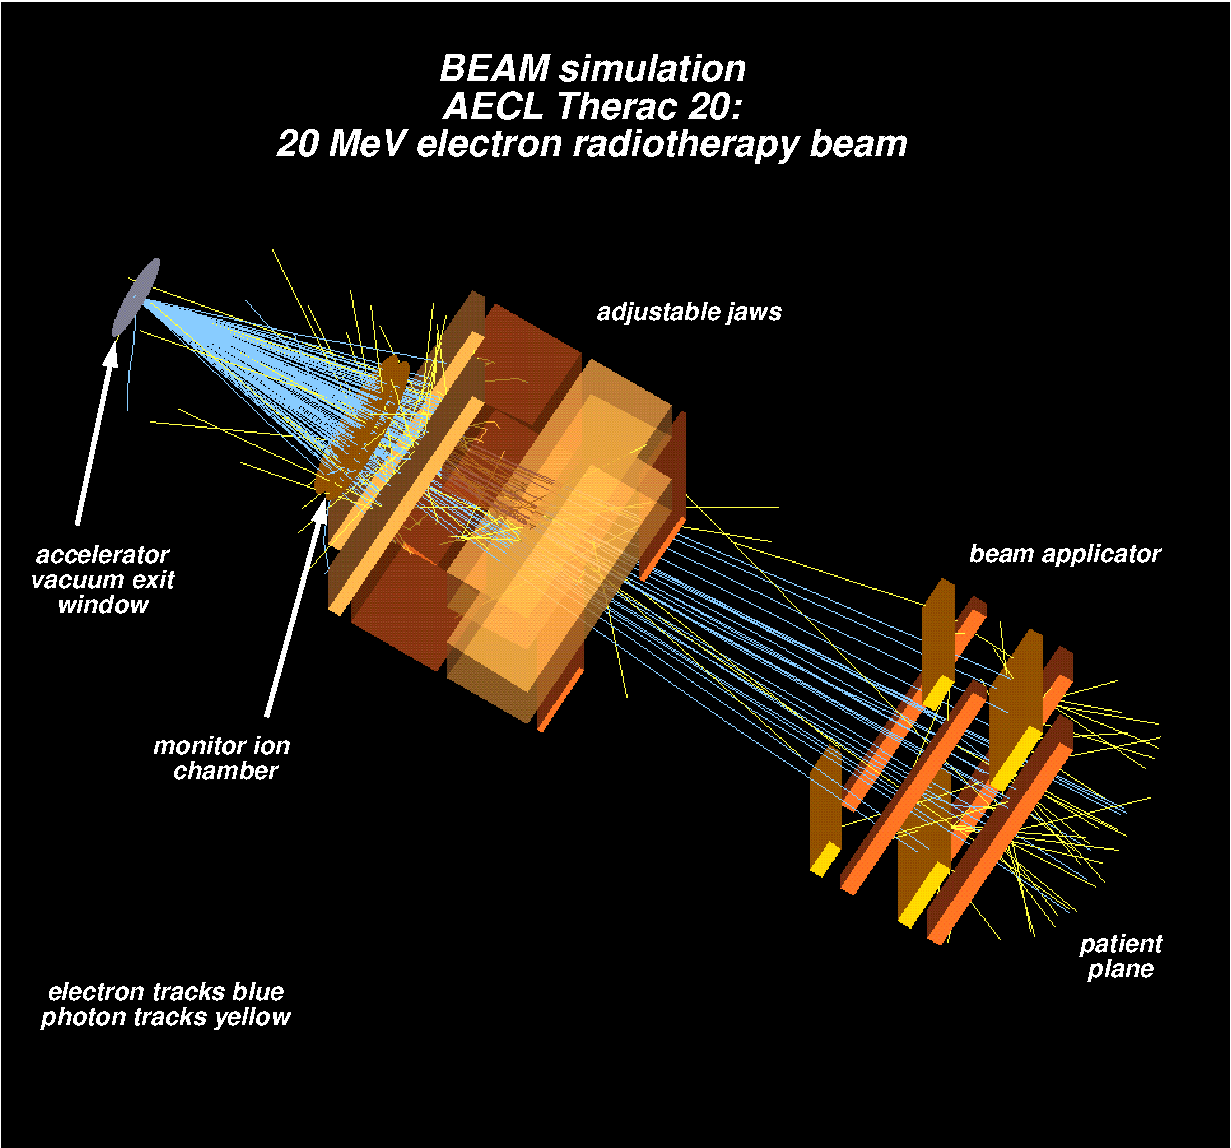
\includegraphics[height=14cm]{figures/th20_20-new}
\end{center}
\end{figure}

\begin{center}

\vfill
\copyright NRC Canada, 2015
\end{center}

\setlength{\baselineskip}{0.5cm}
\newpage

\pagestyle{fancy}
\pagenumbering{arabic}
\setcounter{page}{2}


\newpage

\begin{center}
\begin{Large}
{\bf Abstract}
\end{Large}
\end{center}
\index{abstract}
BEAMnrc is a Monte Carlo simulation system (Med. Phys. {\bf 22},1995,503 --
524) for modelling radiotherapy
sources which was developed as part of the OMEGA project to develop 3-D
treatment planning for radiotherapy
(with the University of Wisconsin).  BEAMnrc is built on the
EGSnrc Code System\cite{KR03}.  Until 2004, BEAMnrc could only
be run on Unix/Linux systems.  However, with the recent port
of BEAMnrc to the EGSnrcMP system\cite{Ka03}, BEAMnrc can also
run on Windows-based systems.
The purpose of this manual is to be a reference/guide to someone
using the BEAMnrc system.

This user's manual covers general BEAMnrc inputs and component module (CM)
geometries and inputs. It discusses how to use the various variance
reduction techniques which are part of the system, most importantly,
range rejection, bremsstrahlung splitting, photon forcing in a specific
region and Russian Roulette.
It also covers the structure of the directory system used for the
BEAMnrc system, the utility codes available (readphsp, addphsp, checkCM8 \etc),
the installation procedure, the phase space file definition and it
has cross references to all related BEAMnrc documentation.
Appendix A gives a specification for writing new component
modules.
\vspace*{4cm}\\

\tableofcontents

\listoffigures

\setlength{\baselineskip}{0.5cm}

\newpage

%\pagestyle{myheadings}

\section{Overview of BEAMnrc}

An extensive paper describing the BEAM system and its application has
been published (ref~\cite{Ro95}) and it is assumed that the user is
familiar with that paper which is also available on-line at
\htmladdnormallink{
{\sf http://www.physics.carleton.ca/~drogers/pubs/papers/Ro95.pdf.}}
{http://www.physics.carleton.ca/~drogers/pubs/papers/Ro95.pdf}
\index{BEAMnrc!paper on-line}
\index{on-line!BEAMnrc paper}
We draw attention to the index in the present document
since a great deal of effort has gone
into making it and we find it a useful way to find information in this
manual.  This manual was originally written before the BEAM graphical
user interface (GUI) was developed\cite{Tr04} and, thus, those sections
describing input formats are somewhat redundant since the GUI makes the
formatting of the input much easier. The EGSnrc
system\cite{Ka99a,KR03,Ro00} was released in February 2000 and the BEAM
code system was ported to using EGSnrc in 2001, used at the course in
October 2001 and generally released in Feb 2002. In spring 2004 a version
of the code was released to course participants with Directed Brem
Splitting available. In fall 2004 this version of the code was made
available generally with a port to the EGSnrcMP system which allows the
code system to be run on Windows systems as well as the traditional
Unix/Linux systems. There is a `new version'
of this manual with each release of the code (usually with the annual
course) and there have been five major
revisions\cite{Ro95b,Ro97,Ro98a,Ro01b,Ro04} with changes in authorship to
represent those primarily responsible for the current version.
\index{BEAMnrc GUI} \index{GUI}

\subsection{The Physics in BEAMnrc}

BEAMnrc uses the EGSnrc Monte Carlo system of radiation transport.  The
physics in EGSnrc is described in detail in the EGSnrc manual
\cite{KR03}.  The transport physics in EGSnrc is greatly improved
over that in EGS4 (the basis for all BEAM versions up to and including
BEAM00).  Among the improvements are the ability to include relativistic
spin effects in elastic scattering cross-sections for electrons, the ability
to simulate atomic relaxations after Compton and photoelectric events and
improved electron transport and multiple scattering algorithms.
All these improvements increase the accuracy of EGSnrc over EGS4, especially at lower energies.
The user has control over the extent to which the new physics is used in
a simulation and also over some parameters required for the new physics.  This
means there are additional inputs for BEAMnrc that did not exist in
previous versions of BEAM.   On the other hand, the introduction of EGSnrc
has eliminated the need for PRESTA and its associated inputs. Also,
the EGSnrc inputs supersede some of the main BEAM inputs
(such as {\tt IDORAY} for controlling Rayleigh scattering, and
{\tt IFLUOR} for turning on K-shell X-ray fluorescence).  See
section~\ref{egsnrc_inputs} for a full description of the EGSnrc inputs
and a more detailed description of the improved physics.  The default
EGSnrc parameters used by BEAMnrc were selected to balance efficiency and
accuracy for typical accelerator simulations so,
\eg, the EGSnrc default {\tt EXACT} boundary crossing algorithm (BCA) is
used instead of the faster {\tt PRESTA-I} BCA because the latter has
been shown to result in significant overestimates of dose when the
CHAMBER component module is used as a phantom\cite{WK06}, however,
atomic relaxations in BEAMnrc default to ``off'' (default in EGSnrc is ``on'')
because their effect is insignificant at accelerator energies.

BEAMnrc retains compatibility with older BEAM input files that do not
include EGSnrc inputs.  In this case, the EGSnrc parameters simply
revert to the default values used in BEAMnrc which differ from the EGSnrc
defaults (see section~\ref{egsnrc_inputs}).
\index{physics in BEAMnrc}
\index{EGSnrc}


\subsection{Other documents available}
\label{oda}
\index{documentation!other}

There are several other documents which describe associated subjects.

\begin{description}

\index{BEAMnrc GUI} \index{GUI}
\item [BEAMnrc, DOSXYZnrc and BEAMDP GUI User's Manual:] Describes how to
install and use these graphical user interfaces to BEAMnrc and
related codes\cite{Tr04}.

\index{BEAMDP}
\item [BEAMDP as a General-Purpose Utility:] User's manual for using
BEAMDP to do simple analysis of phase space files - presenting spectra,
fluence distributions, average energies, listings, angular distributions
\etc, including the possibility of using the {\tt LATCH} values in the phase
space file\cite{Ma95b}.

\index{QA for BEAMnrc}
\item [QA for the BEAMnrc System:] Component Modules, Variance Reduction
Options and Source Routines. This 100 page document is for internal use
at NRC but describes the extensive QA program carried out on component
modules, variance reduction
options and source routines. It also describes
the automated system for on-going QA\cite{WR95a}.

\index{DOSXYZnrc}
\item [DOSXYZnrc User's Manual:] DOSXYZnrc is an associated code for doing dose
distribution studies in a CT voxel phantom irradiated by a beam
calculated using BEAMnrc\cite{Wa05}.

\item[Specifications for Component Modules for BEAMnrc:] This document is
for code developers who need to know what is going on in
the code so they can write a new CM. It is attached as Appendix
A(section~\ref{appendixA}).
\index{specifications for CMs}
\index{CMs}

\item[EGS\_Windows\_4.0 User's Manual:] User's manual for an X-windows based
display tool for EGS histories and BEAMnrc geometries\cite{TR99a}.
\index{EGS\_Windows\_4.0}

\item[The EGSnrc Code System Manual- PIRS-701:] Complete manual describing
the use of the EGSnrc simulation system\cite{KR03}.

\item[EGSnrcMP: the multi-platform environment for EGSnrc- PIRS-877:] Manual
describing the EGSnrcMP system\cite{Ka03}.  Essential reading to understand
how the current version of BEAMnrc is compiled and run.

\item[History by history statistical estimators in the BEAM code system:]
Med Phys {\bf 29} (2002) 2745--2752: In-depth description of the method used
to estimate uncertainty in BEAMnrc and DOSXYZnrc\cite{Wa02a}.

\item[Large efficiency improvements in BEAMnrc using directional
brem splitting:~~~] Med Phys {\bf 31} (2004) 2883 -- 2898. Describes
major improvement in efficiency for photon beam simulations\cite{Ka04a}.
\index{DBS} \index{Directional bremsstrahlung splitting}


\end{description}


\subsection{Overview of the directory structure}
\label{dirstructsect}

\index{directory structure!OMEGA\_HOME}
\index{overview!directory structure}
The OMEGA/BEAM system has a well defined structure of directories.  It
can be thought of as having two or possibly three general parts.  The
first sub-system is generally referred to as \verb+$OMEGA_HOME+ and
contains all the source code needed to run BEAMnrc and
associated codes such as readphsp, BEAMDP \etc.   In practice
\verb+$OMEGA_HOME+ is the directory {\tt \$HEN\_HOUSE/omega} (more
about {\tt \$HEN\_HOUSE} below).  Figure
~\ref{fig_omega_home} outlines the \verb+$OMEGA_HOME+ subsystem.
Note that this part of
the system contains no execute modules related to beam simulation.
These all reside on the user's {\tt \$EGS\_HOME} area described below.

\index{OMEGA\_HOME}
\begin{figure}[hbp]
\begin{center}
\leavevmode
\mbox{}\hspace{0cm}
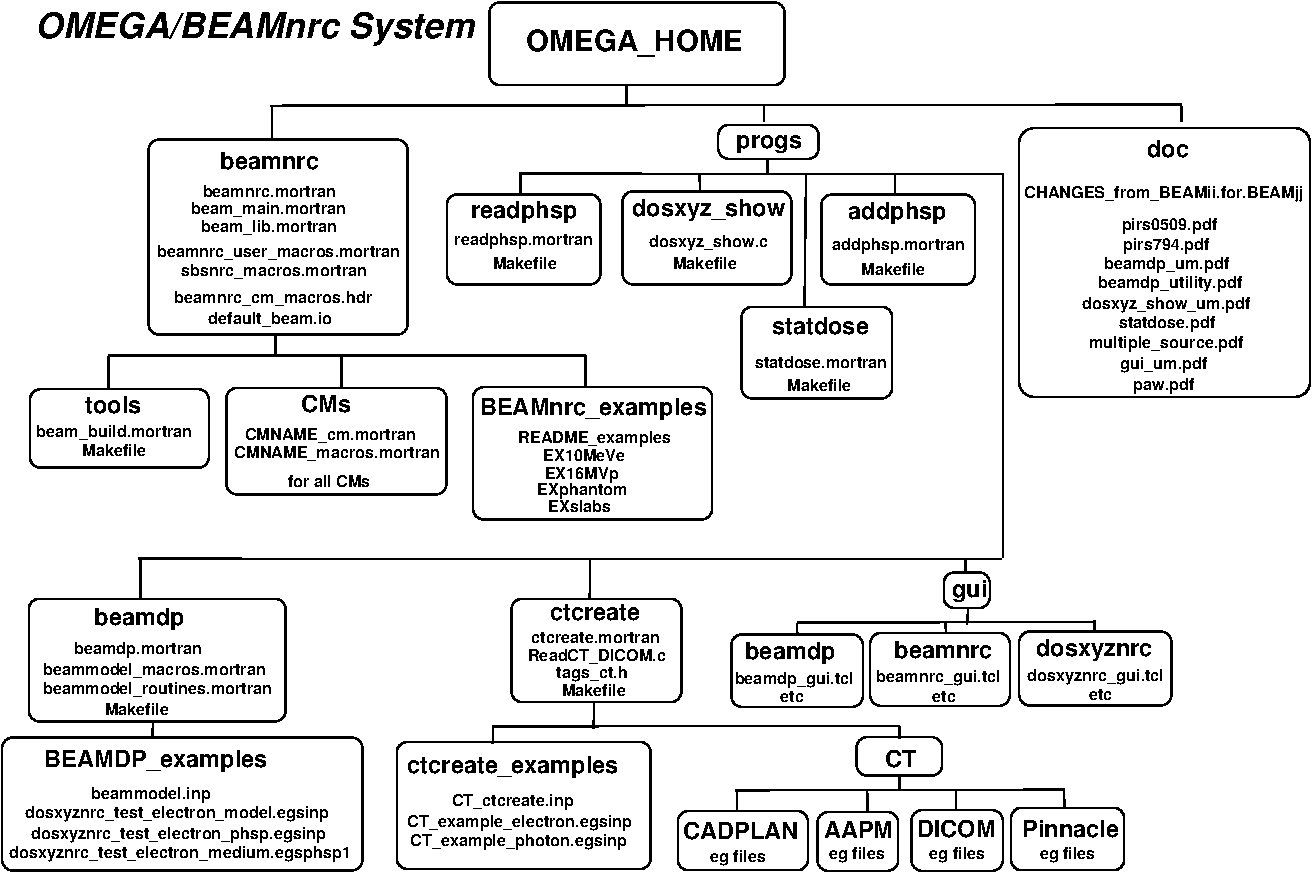
\includegraphics[width=17cm]{figures/omega_home}
\index{OMEGA\_HOME}
\caption[Components of {\tt \$OMEGA\_HOME} subdirectory.]
{Main components of the {\tt \$OMEGA\_HOME} directory.
{\tt \$OMEGA\_HOME} is a subdirectory, called {\tt omega}, of
{\tt \$HEN\_HOUSE} which is given in fig~\ref{fig_hen_house}}
\label{fig_omega_home}
\end{center}
\index{beamnrc.mortran}
\index{OMEGA\_HOME}
\index{progs}
\index{CMs}
\end{figure}

{\tt \$OMEGA\_HOME} resides (as directory {\tt omega})
within the {\tt \$HEN\_HOUSE}, which contains the EGSnrcMP system.
This is shown in more detail in fig~\ref{fig_hen_house}.
\index{examin}
\index{directory structure!HEN\_HOUSE}
\begin{figure}[hbp]
\begin{center}
\leavevmode
\mbox{}
\hspace*{-1cm}
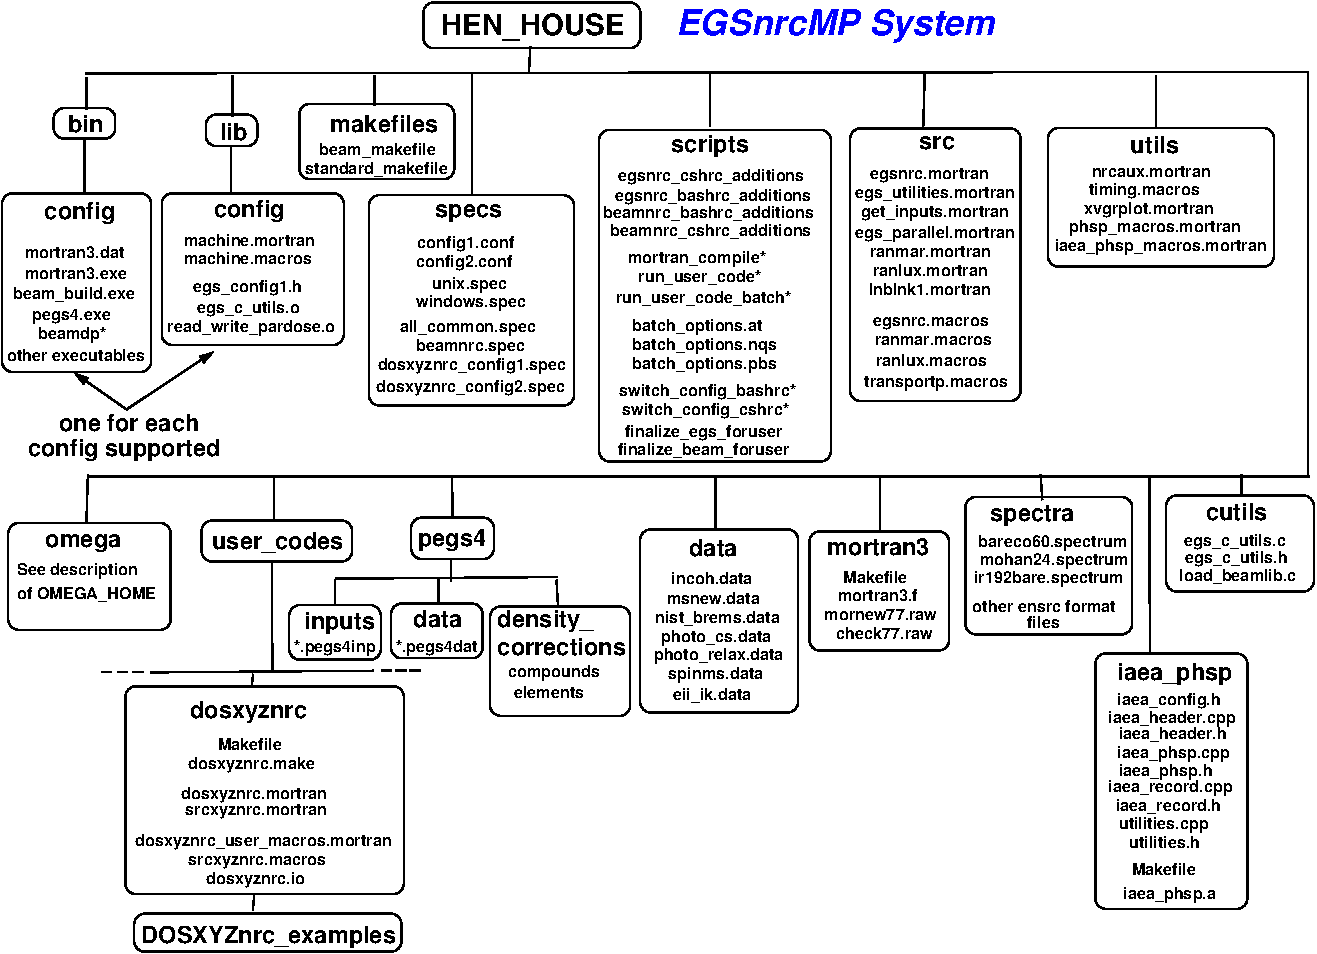
\includegraphics[width=19cm]{figures/hen_house}
\caption[Structure of EGSnrcMP directory, {\em i.e~} the {\tt \$HEN\_HOUSE}.]
{The structure of the
EGSnrc system. Note that the {\tt \$OMEGA\_HOME} subsystem shown in
fig~\ref{fig_omega_home} is included in this structure.
}
\index{HEN\_HOUSE} \index{NRC EGSnrcMP system}
\label{fig_hen_house}
\end{center}
\end{figure}
\index{HEN\_HOUSE}
Originally, EGSnrc was a Unix-based script system developed primarily by
Alex Bielajew and Dave Rogers at NRC.  With the advent of EGSnrcMP\cite{Ka03}
and the
requirement for compiling on Windows-based systems in addition to Unix-based
systems, we have largely eliminated the scripts and, in the case of
compilation, replaced them with the GNU {\tt make} utility.
For more detail about the EGSnrcMP system and how it works, see the
EGSnrcMP manual~\cite{Ka03}.  For users of the previous BEAM/BEAMnrc
systems, note that in the past the {\tt \$HEN\_HOUSE} was a component of
{\tt \$OMEGA\_HOME} since the EGS system was distributed as a component of
BEAM whereas in the EGSnrcMP system, BEAMnrc is  a special subcomponent of
{\tt \$HEN\_HOUSE} and DOSXYZnrc is treated as just another user-code.

The final component of the OMEGA/BEAM structure is the user's area which
is shown in fig~\ref{fig_users_area}.  This is known as {\tt \$EGS\_HOME}
and is usually the subdirectory {\tt \$HOME/egsnrc\_mp}.  The BEAM
installation will set
\index{directory structure!users area}
\index{user's area}
\begin{figure}[hbpt]
\htmlimage{scale=2.0}
\leavevmode
\begin{center}
\mbox{}\hspace{0cm}
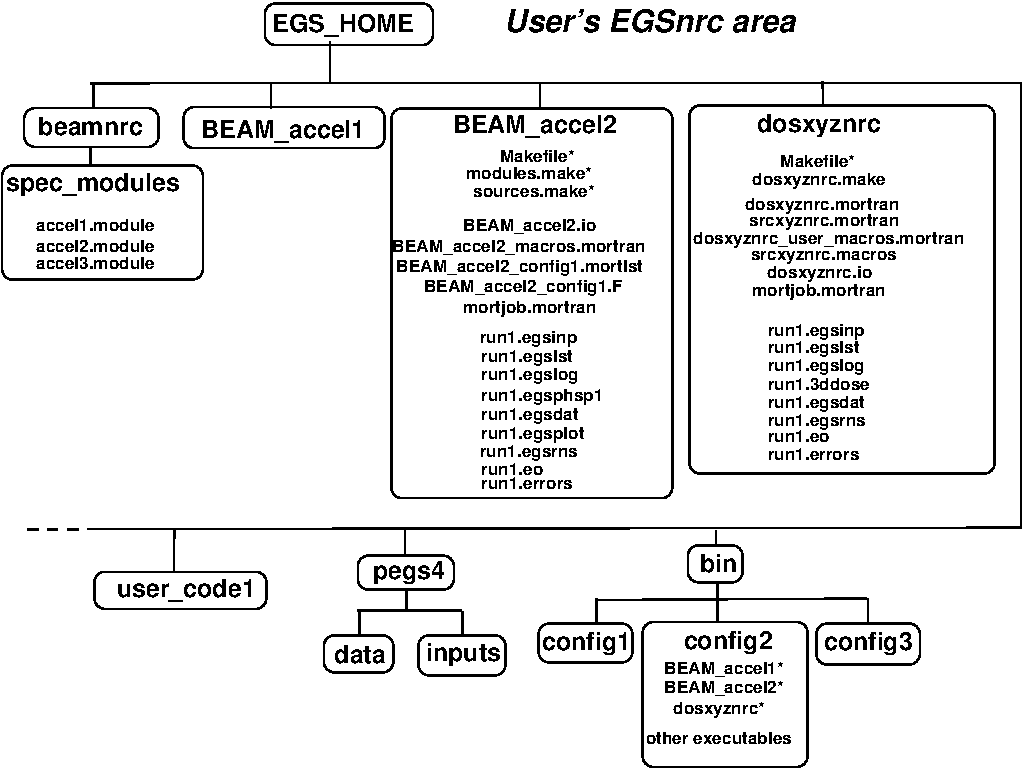
\includegraphics[width=17cm]{figures/nrc_users_area}
\index{user's area}
  \caption[The user's \$EGS\_HOME area.]{The user's {\tt \$EGS\_HOME}
  area (usually {\tt \$HOME/egsnrc\_mp}).  A $*$ indicates an executable
  file. In the example shown, the user has 3 accelerator models and the
  disk system is being used with three different configurations, \eg, gcc,
  pgf77 and Windows.  The complete directory contents are only shown
  for accel2 and config2.  Other EGSnrc user codes (eg DOSXYZnrc) also
  reside in the {\tt \$EGS\_HOME} area.}
\label{fig_users_area}
\end{center}
\end{figure}
up much of this automatically if it is not in place.
One of the main complications is that the
EGSnrcMP and BEAMnrcMP systems are
set up to use one disk system to support multiple configurations and
their associated compilers.
\index{multiple configurations}
\index{script!egsnrc}
Thus, all execute modules and various compiler options
\etc~ must be handled separately for each configuration.
Within the \verb+bin+ area, the modules within
each subdirectory apply only to the configuration shown.

\clearpage
\subsection{Overview of running BEAMnrc}

\index{overview}
Figure~\ref{fig_flow} presents a schematic of the overall steps required
to do an accelerator simulation.  At the {\sf specify} accelerator and {\sf
build} accelerator steps, the user is instructing the system how to pull
together the source code and make an execute module.  At this stage, only a
\index{specifying accelerators} \index{building accelerators}
\index{overview!running BEAMnrc}
\index{BEAMnrc!flow diagram}
\begin{figure}[htbp]
\begin{center}
\leavevmode
\mbox{}\hspace{0cm}
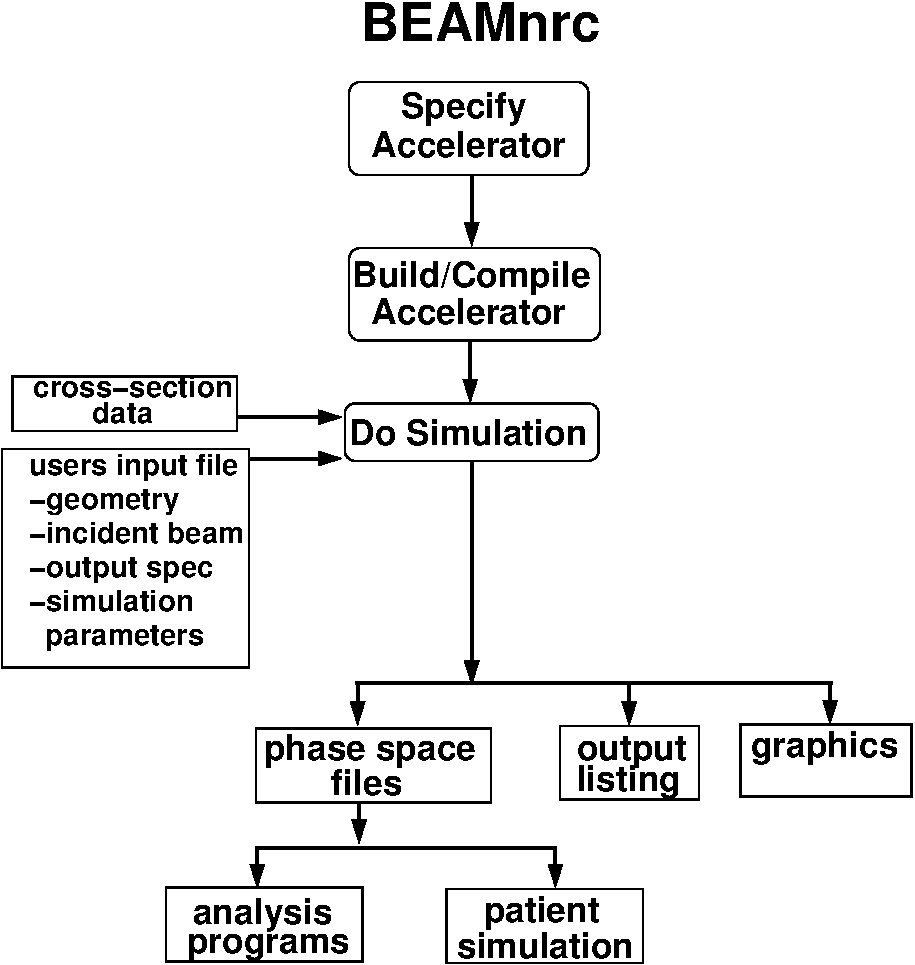
\includegraphics[width=15cm]{figures/flow}
\index{building accelerators}\index{specifying accelerators}
\caption[Steps involved in using the BEAMnrc code]
{The steps involved in using the BEAMnrc system, from ref~\cite{Ro95}.}
\label{fig_flow}
\end{center}
\end{figure}
broad class of accelerator is defined (\eg\ whether the flattening
filter is before or after the primary collimator).  During the execution
stage, the program reads in a large quantity of data related to photon
and electron cross sections for the specific materials in this
accelerator model. These data are generated by a code,
called PEGS4 (which is included with the EGSnrc system
see section~\ref{CSDP}) or read from data files such as
{\tt msnew.data}, {\tt spinms.data}, etc,  which are contained in the
{\tt \$HEN\_HOUSE/data} subdirectory. Also the user creates an input file
which specifies
all the details about the particular accelerator (\eg, there are 4 scattering
foils located at specified distances from the vacuum exit window,
made of certain materials and of particular thickness).  Also the user
must specify all the parameters controlling the radiation transport
modelling and must also select and control the various variance
reduction techniques being used.

The final stage of the simulation is the analysis of the outputs which
consist of raw phase space files (measured in tens if not hundreds of
Mbytes), an output listing and optionally a 3D graphics file to be displayed
by {\tt EGS\_Windows}\cite{TR99a}.
\index{EGS\_Windows}

\section{Building/compiling/running BEAMnrc}

See section~\ref{installbeam} at the end of this manual for
instructions for installing BEAMnrc and the rest of
the OMEGA/BEAM codes.

\index{.cshrc}
\index{egsnrc\_cshrc\_additions}
\index{egsnrc\_bashrc\_additions}
\index{.bashrc}
If you have installed BEAMnrc on a Linux/Unix system then the first
step towards running the code is to go into your {\tt \$HOME/.cshrc}
or {\tt \$HOME/.bashrc} (depending on whether you're running in a C-shell
or Bourne-shell, respectively) file and, at the end of the file, add the
following statements:
\index{EGS\_HOME}
\index{EGS\_CONFIG}
\begin{verbatim}
setenv EGS_HOME /full directory path to $HOME/egsnrc_mp/
(or export EGS_HOME=/full directory path to $HOME/egsnrc_mp for .bashrc)
setenv EGS_CONFIG /full directory path to $HEN_HOUSE/specs/config.conf/
(or export EGS_CONFIG=/full directory path to $HEN_HOUSE/specs/config.conf/
                                                              for .bashrc)
source /full directory path to $HEN_HOUSE/scripts/egsnrc_cshrc_additions
(or source /full directory path to $HEN_HOUSE/scripts/egsnrc_bashrc_additions
                                                              for .bashrc)
\end{verbatim}
where {\tt config} is the name of the particular configuration
(eg {\tt gcc}, {\tt pgf77}) that you have installed BEAMnrc on.  The
first three statements are required for the
EGSnrcMP system (see the EGSnrcMP Users Manual\cite{Ka03}), while
{\tt \$HEN\_HOUSE/scripts/egsnrc\_cshrc\_additions}
(or {\tt \$HEN\_HOUSE/scripts/egsnrc\_cshrc\_additions}) define aliases
for the OMEGA/BEAM system.  Once you have added these statements you
must source the {\tt .cshrc}
(or {\tt .bashrc}) file to bring them into effect.

Instructions for adding these statements are given explicitly at the
end of the EGSnrcMP and BEAMnrc installations (see section~\ref{installbeam})

No such additions are required when installing BEAMnrc on a Windows system.

Previous to the current version of BEAM (BEAMnrcMP), the user had the
option to specify, build, compile and run a BEAM simulation
from within a Linux/Unix script, called {\tt beamnrc}. \index{beamnrc script}
This script was eliminated with the advent of BEAMnrcMP as it was seen to
be of limited use for a system that is also required to work on
Windows (which does not support scripts).  However, you will note
in the descriptions that follow that all of the functions of the
{\tt beamnrc} script can be performed (in a much more user-friendly
manner) from within the BEAM GUI.

\subsection{``Specifying'' Accelerators}
\index{specifying accelerators}
\index{accelerator!specifying}

Before compiling and running a BEAM accelerator simulation, you must
``specify'' which component modules are to be used and in what order.
The available
\verb+CMs+ are discussed in detail in section~\ref{CMs}.  Each CM can be
used in a wide variety of applications and user should not restrict
themselves by the names. For example, the JAWS CM is well suited to
simulating a wedge.  It is useful to select identifiers (8 characters or
less) which are physically meaningful (eg xit\_win, scatfoil, jaws \etc)
since these will appear throughout the code and listing files and thereby
help the user understand
what is going on in various applications.  The user may use the same CM
as often as needed, as long as the identifiers used are unique.
One restriction is that the identifier name should not start with the
word ``exit'' since the \verb+MORTRAN+ compiler gets confused with this.
\index{accelerator!identifiers}
\index{identifiers}
\index{identifiers!exit}

\index{.module files}
Accelerators are stored in a very simple format in
{\tt myaccel.module} files that reside in the
user's {\tt \$EGS\_HOME/beamnrc/spec\_modules} subdirectory (see
Figure~\ref{fig_users_area} above).  When built and compiled, the
executable code will have the name {\tt BEAM\_myaccel}, so
it is useful to have {\tt myaccel} indicate the machine you are
modeling.

The {\tt myaccel.module} file created from scratch using the
BEAM GUI (just select ``Specify a new accelerator" from the ``File"
menu), or you can copy an existing {\tt .module} file (eg one of the
examples included with the distribution) into {\tt myaccel.module}
and modify the latter for your own purposes using an editor.

Any number of specified accelerators can coexist at the same
time.

\subsection{Building an Accelerator: The {\tt beam\_build} Code}
\label{beambuildsect}
\index{building accelerators}
\index{accelerator!building}
\index{beam\_build}

Once the accelerator has been specified, it must be ``built'', which
corresponds to concatenating all of the relevant source code for the
\verb+CMs+
and editing it to avoid duplicate variable names
(this is discussed below for
those who need details).  The resulting files are on the user's area and
are
\verb+$EGS_HOME/BEAM_myaccel/BEAM_myaccel_cm.mortran+ and \\
\verb+$EGS_HOME/BEAM_myaccel/BEAM_myaccel_macros.mortran+.
Note that the name of the subdirectory and the file names themselves
\index{prefix} \index{BEAM\_}
are just the name of the specification module with the prefix \verb+BEAM_+.

If you are modifying the code at all, an accelerator must be re-built
every time any of the  \verb+CMs+ are modified, but not when the main
\verb+beamnrc.mortran+ code is modified.

An accelerator is built using the MORTRAN code {\tt beam\_build.mortran}.
The command for running this code to build the accelerator specified
by {\tt myaccel.module} is:
\begin{verbatim}
beam_build.exe myaccel
\end{verbatim}
\index{beam\_build.exe}
{\tt beam\_build.exe} creates the
{\tt BEAM\_myaccel\_cm.mortran} and {\tt BEAM\_myaccel\_macros.mortran} files
and puts them in the {\tt BEAM\_myaccel} subdirectory (creating the subdirectory
on the way if it does not already exist).

\index{Makefile}
\index{modules.make}
\index{sources.make}
In addition, {\tt beam\_build} creates
the files {\tt Makefile}, {\tt modules.make} and {\tt sources.make} and
puts them in the {\tt BEAM\_myaccel} subdirectory.  These files
are used for compiling beam.
More details
are given in section~\ref{makefilesect}, on
page~\pageref{makefilesect}, below.

If the {\tt beam\_build} utility has not already been compiled for your particular
configuration (this may be the case if you have switched configurations
after installing BEAMnrc), then before typing the above command line, go into
{\tt \$HEN\_HOUSE/omega/beamnrc/tools/beam\_build} and type {\tt make}.  This
will put a copy of the {\tt beam\_build.exe} executable in the appropriate
subdirectory of {\tt \$HEN\_HOUSE/bin}.

\subsection{Compiling an Accelerator using {\tt make}}
\label{ca}
\index{compiling!using make}

Once specified and built, the accelerator must be compiled. This
\index{MORTRAN}
requires using the \verb+MORTRAN+ compiler (which is supplied as part of
the EGSnrc system) followed by the \verb+FORTRAN+ compiler.
\index{Fortran}

\index{make}
In previous versions of BEAM, compiling of accelerators was completely
driven by Unix scripts.  However, with the necessity to run on non-Unix
platforms, EGSnrcMP now uses the GNU
{\tt make} utility.  For more detailed information on {\tt make}, see
the EGSnrcMP manual~\cite{Ka03}.

To compile an accelerator, go into the {\tt BEAM\_myaccel}
subdirectory and type:
\begin{verbatim}
make [options]
\end{verbatim}

The options for {\tt make} are:
\index{make!options}
\begin{verbatim}
make              Compile the accelerator executable with default optimization
make opt          turned on.  Default optimization is level 3 (-O3).

make noopt        Compile the accelerator executable with optimization
                  turned off.

make debug        Compile an accelerator executable for debugging.

make fortran      Do mortran compilation only, leaving behind the fortran
                  file BEAM\_myaccel\_config.F.

make clean        Remove the fortran file, mortjob file, mortlst file
                  and the various executables.
\end{verbatim}

Upon typing {\tt make} you will see output to the screen indicating files
that are being concatenated together to create the final .mortran code
that is then compiled.

After compiling an accelerator, the following files will be left behind:
\index{make!targets}
\begin{description}
\item In the accelerator directory:
\begin{description}
\index{mortjob.mortran}
\item[{\tt mortjob.mortran}] The concatenated MORTRAN file which is MORTRAN
compiled.
\index{.mortlst file}
\item[{\tt BEAM\_myaccel\_config.mortlst}] Listing from the MORTRAN compiler.
Contains the concatenated MORTRAN code, formatted with levels of
loops and {\tt IF} blocks indicated.  Output at the end of the file indicates
if there were any MORTRAN errors and, if so, how many and of what type.
\index{Fortran code}
\index{C routines}
\item[{\tt BEAM\_myaccel\_config.F}] Fortran output from the MORTRAN compiler.
This is the f77 code that is ultimately Fortran compiled.  The use of
capital ``F" indicates that some C routines are to be linked with the
Fortran code at compile time.  In the case of BEAM, these C routines pertain
to parallel job submissions.
\end{description}
\item In the {\tt \$EGS\_HOME/bin/config} directory:
\begin{description}
\index{executable code}
\item[{\tt BEAM\_myaccel*}] The executable code.
\end{description}
\end{description}

If none of the MORTRAN source coding or macros have changed since the last
compilation and the file {\tt BEAM\_myaccel\_config.F} exisits in the
accelerator directory and there is an executable in your
{\tt \$EGS\_HOME/bin/config} directory, then typing {\tt make} will not recompile
the accelerator.

If you want to include the beam characterization source in the accelerator,
see the instructions in section~\ref{Source31} page~\pageref{Source31}.

\subsubsection{Compiling an Accelerator as a Shared Library}
\label{sharedlibsect}
\index{compiling an accelerator!as a shared library}
\index{shared library!accelerator}

DOSXYZnrc\cite{Wa05} and other EGSnrc user codes\cite{Ro03} allow the user
to use a full BEAM simulation as a particle source (instead of a stored phase space
file).  In order to use this source, the BEAM accelerator code must first
be compiled as a shared library.

Once an accelerator has been built,
it can be compiled
as a shared library by going into {\tt \$EGS\_HOME/BEAM\_myaccel} and
typing:
\index{make!library}
\begin{verbatim}
make library
\end{verbatim}
\index{mortjob.mortran}
The codes concatenated to create the {\tt mortjob.mortran} file are the same
as those used for a standard BEAM compilation with the exception that
\index{beam\_lib.mortran}
\index{beam\_main.mortran}
\\{\tt \$OMEGA\_HOME/beamnrc/beam\_lib.mortran} is used in place of\\
{\tt \$OMEGA\_HOME/beamnrc/beam\_main.mortran} (see
section~\ref{mortjobsect}, page~\pageref{mortjobsect}).
The library compilation also leaves behind
{\tt libBEAM\_myaccel\_config.mortlst} (output from MORTRAN compiler) and
{\tt libBEAM\_myaccel\_config.F} (Fortran source code), where {\tt config}
is the name of your configuration.

\index{libBEAM\_myaccel.so}
\index{BEAM\_myaccel.dll}
The BEAM shared library is archived as the file {\tt libBEAM\_myaccel.so} (for
unix/Linux machines) or {\tt BEAM\_myaccel.dll} (for Windows machines) in
directory {\tt \$EGS\_HOME/bin/config}.

Note that previous versions of BEAMnrc required
\index{libg2c.a}
the static g2c library, {\tt libg2c.a}, when compiling shared
libraries on Unix/Linux machines.  Use of this library prevented
confusion of I/O units between BEAM and the code using BEAM as a source
(the ``driving'' code).
In the current version of BEAMnrc, however, the opening of I/O units
has been recoded so that only those units not already being used by
the driving code are available to BEAMnrc.

When using the BEAM shared library as a source, you must also supply
a working input file and the pegs data for the BEAM simulation.  The input
file must exist in your {\tt \$EGS\_HOME/BEAM\_myaccel} directory and
be set up to write a phase space file at a scoring plane.  See the
DOSXYZnrc Manual\cite{Wa05} and the manual for EGSnrc user codes\cite{Ro03}
for more details about this source.

\subsection{Compiling an Accelerator using {\tt mf} (Unix/Linux specific)}
\index{compiling}
\index{mf}
\index{compiling!with mf}
To preserve compatibility with old usage, an accelerator can also be
compiled using {\tt mf}, which is aliased to the Unix script
{\tt \$HEN\_HOUSE/scripts/compile\_user\_code}.  To compile using
{\tt mf}, go into the {\tt BEAM\_myaccel} directory and type:

\begin{verbatim}
m[f] BEAM_myaccel [a] [opt|noopt|debug]
\end{verbatim}
\index{mf!options}
The options for {\tt mf} are:
\verb+mf         =>+ Mortran and Fortran compile and then link\\
\verb+m          =>+ Mortran compile and create the Fortran file\\
\verb+opt        =>+ use optimization\\
\verb+noopt      =>+ use no optimization\\
\verb+debug      =>+ create executable ready for a debug run\\
The parameter ``{\tt a}" is not used and is only present for compatibility
with the previous version of {\tt mf}.

Once the {\tt mf} command is issued, the {\tt compile\_user\_code}
script then calls {\tt make} with the appropriate options.

\subsection{Building/Compiling with the BEAM GUI}
\index{compiling!with the GUI}
Building and compiling are done in a single step when using the BEAM GUI.
Once an accelerator {\tt .module} file has been specified or read into
the GUI, then it can be built/compiled by selecting ``Compile" from
the ``Execute" menu.  This opens up a window in which you can choose any
of the {\tt make} options outlined in section~\ref{ca} above.  Then
press the ``BUILD \& COMPILE" to run {\tt beam\_build} followed by
{\tt make}.  If there
is no {\tt beam\_build.exe*} executable in the appropriate
{\tt \$EGS\_HOME/bin/config} directory, then the GUI will automatically
compile {\tt beam\_build} for your configuration.

\subsection[Internal Documentation \& Input Description]{Internal Documentation and Input Description}
\index{documentation}
\index{input description}

Since a given accelerator model can have an arbitrary structure,
defining the input file for a given accelerator must be done after the
accelerator is specified.
Extensive descriptions of the main BEAM inputs and individual CM inputs
are given at the top of the {\tt beamnrc.mortran} and {\tt CM\_cm.mortran}
codes, however the BEAMnrc graphical user interface (GUI) provides
extensive descriptions of each input variable in addition
to being able to display graphical representations of component module and
accelerator geometries as input by the user.
Thus, the GUI is the preferred method for generating
input files.  For more information on the BEAMnrc gui, see the BEAMnrc,
DOSXYZnrc and
BEAMDP GUI User's Manual\cite{TR99}.
\index{BEAMnrc GUI} \index{GUI}

\subsection{Running an Accelerator Simulation}
\index{running a simulation}
\index{accelerator!simulation}

Once the accelerator model is compiled, the user may run a simulation.
To run a simulation from the command line, type:
\index{command for running BEAMnrc}
\index{input file}
\index{pegs data file}
\begin{verbatim}
BEAM_myaccel -i inputfile -p pegsdata
\end{verbatim}
where {\tt inputfile} is the name of the BEAM inputfile (with no
{\tt .egsinp} extension) and {\tt pegsdata} is the name of the PEGS4
material data file (with no {\tt .pegs4dat} extension).  These two
files are discussed in more detail below.

\index{running BEAMnrc! with Unix script}
\index{ex}
To preserve compatibility with old usage, accelerators can also be run
with the ``{\tt ex}" command:
\begin{verbatim}
ex BEAM_myaccel inputfile pegsdata
\end{verbatim}
``{\tt ex}" is aliased to the Unix script {\tt \$HEN\_HOUSE/scripts/run\_user\_code}.  This script uses the non-script command line shown above to
actually run the accelerator, but first it checks for the existence of
the relevant directories ({\tt \$EGS\_HOME} and the {\tt BEAM\_myaccel}
subdirectory).  It also
checks for the existence of the
{\tt BEAM\_myaccel*} executable and compatibility between the
{\tt config.conf} file you are using and the actual configuration that
you are running on.

\index{input file}
\index{.egsinp}
The users input file, \ie\ \verb+inputfile.egsinp+, defining the geometry
of the accelerator and the BEAM simulation parameters, must exist
in \verb+$EGS_HOME/BEAM_myaccel+.  The best way for a new user to begin
creating a new input file is to use the BEAM GUI\cite{TR99}.
\index{BEAMnrc GUI} \index{GUI}  From the GUI, you can either begin a new
input file from scratch or read in an existing input file (for the same
accelerator) and modify the parameters accordingly.  More experienced users
may find it faster to use an editor to modify an existing input file.

Note that the input file extension is {\tt .egsinp}.  Theoretically, BEAMnrc
can run a BEAM00 {\tt .egs4inp} input file, however, depending on the
parameters, there may be new inputs that will cause an error on reading
the older file.  It is safer to read the old {\tt .egs4inp} file
into the GUI and resave it.  The GUI will then write to the file all the necessary inputs for
the current version of BEAM.  Note that {\tt .egs4inp} files do not
contain any EGSnrc transport parameter inputs, so standard BEAMnrc
defaults for these parameters will be used when older files are read
into the GUI and/or used in a BEAM simulation.
\index{EGSnrc - EGS4 conversion}

Much of the rest of this document is devoted to discussing the meaning
of all the options available through the input file.

\index{PEGS4}
\index{cross section data}
In order to run an accelerator, you also have to enter the name
of the {\tt .peg4dat} file containing the cross section data for the
materials in the model.  Note that all of the material names used
in the input file must exist in the {\tt .pegs4dat} file used.
There is more information in section~\ref{CSDP}
but basically
the files \verb+700icru.pegs4dat+ and \verb+521icru.pegs4dat+
\index{.pegs4dat}\index{700icru.pegs4dat}\index{521icru.pegs4dat}
contain data for a large number of
commonly used materials. The numbers in the names correspond to AE=521
\index{AE}
and AE=700, \ie\ thresholds for secondary electron production of 10 and
189 keV kinetic energy respectively. The data sets go up to 55 MeV in
both cases.  These data sets are on the distribution on area
\verb+$HEN_HOUSE/pegs4/data+.  If the user wishes to make their own data
files using the program PEGS4,
these files can be put either on that area, or on the user's pegs4
area, \viz\ \verb+$EGS_HOME/pegs4/data+.

\subsubsection{Batch Runs}
\label{batchsect}
\index{batch runs}
\index{running BEAMnrc!batch runs}

Thus far, we have described interactive BEAM runs, in which the BEAM
input and job execution information is echoed to the screen and where
the window in which the job is running cannot be used for anything else
while the job is executing.  However, if you are running on a Unix/Linux
system, then it is often desirable to run simulations in batch mode.
For example, batch
job submission can make use of a network queuing system
\index{PBS}
\index{NQS}
\index{parallel jobs}
(eg PBS or NQS) and is required for parallel jobs
(see section~\ref{parallelcalc} in this manual for more information
on parallel jobs).

\index{exb}
Submitting a batch job uses the {\tt exb} command, which is aliased
\index{egs\_batch\_run}
to the Unix script {\tt \$HEN\_HOUSE/scripts/run\_user\_code\_batch}.  The
syntax of the {\tt exb} command is:
\begin{verbatim}
exb BEAM_myaccel inputfile pegsdata [short|medium|long] [batch=batch_system] [p=N]
\end{verbatim}

The input {\tt [short|medium|long]} determines the name of the queue to be used
(the default is {\tt long}).  With our naming system at the NRC,
the {\tt short} queue
has the lowest maximum CPU time but the highest priority, while {\tt long} has
an unlimited CPU time with lowest priority.

The {\tt batch=batch\_system} input
determines the name of the queuing system to use.  The
{\tt run\_user\_code\_batch} script sources the file
\index{batch\_options.batch\_system}
{\tt \$HEN\_HOUSE/scripts/batch\_options.batch\_system}, which defines
the batch submission commands for the particular queuing system chosen
and may redefine the names of the queues available on that system
(this means that the queue names {\tt short|medium|long} are not
necessarily general).  Currently, {\tt batch\_system} can be set to
\index{at}
\index{PBS}
\index{NQS}
{\tt at} (the standard Unix batch command), {\tt pbs} (for the
PBS queuing system) or {\tt nqs} (for the NQS queuing system).
This means that the files
\index{batch\_options.at}
\index{batch\_options.pbs}
\index{atch\_options.nqs}
{\tt batch\_options.at}, {\tt batch\_options.pbs} and
{\tt batch\_options.nqs} are included with the EGSnrcMP distribution.  However,
the batch submission commands in these files are for our system at the NRC
and you may have to make some changes for your system.  The default
value for {\tt batch\_system} is {\tt at}, unless you have the environment
\index{\$EGS\_BATCH\_SYSTEM}
variable {\tt \$EGS\_BATCH\_SYSTEM} set to something else.

\index{parallel runs}
Finally, the {\tt p=N} input is used if you want to split the simulation
into {\tt N} parallel jobs.  For more information on parallel runs,
see section~\ref{parallelcalc}, page~\pageref{parallelcalc}.

\index{.egslog}
In addition to the files which are output from an interactive accelerator
simulation, a batch run will also output a {\tt inputfile.egslog} and
file and a
\index{.eo}
{\tt inputfile.eo} file.  The {\tt .egslog} file contains all the output
that would be echoed to the screen during an interactive run.  {\bfseries
IT IS IMPORTANT
TO LOOK AT THE {\tt .egslog} FILE TO SEE IF ANY INPUT OR RUN TIME ERRORS
OCCURRED}.  The {\tt .eo} file contains messages from the queuing system.  If,
for some reason, a job did not get submitted properly, then this file may
contain clues to the problem.  More information on BEAM output files is given
in section~\ref{outputfilessect}, page~\pageref{outputfilessect} below.

For more information on submitting batch jobs, see the EGSnrcMP manual~\cite{Ka03}.

\subsection{Running BEAMnrc using the GUI}
\index{running BEAMnrc!with the GUI}

\index{BEAM GUI}
\index{GUI!BEAMnrc}
It is possible to use the BEAM GUI to submit interactive, and if your
system is set to handle batch jobs, batch and parallel runs.  To do this,
select ``Run" from the ``Execute" menu.  This opens a running window which
will give you the option to switch from an interactive to a batch (and
parallel) run, and will allow you to select the queue you wish to run on.
If you have not set the environment variable {\tt \$EGS\_BATCH\_SYSTEM},
then the GUI automatically submits to a PBS network queuing system (ie
sets {\tt batch\_system=pbs}).  When you press the ``Execute" button, the
GUI then assembles and executes the appropriate command line as described
in the sections above.  Output which would normally appear on the screen
during an interactive run is now displayed in the GUI running window.

\subsection{A Note on Temporary Working Directories}
\label{twdsect}
\index{running directory}
\index{temporary working directory}

Before a BEAM run (batch or interactive), a temporary working directory,\\
{\tt \$EGS\_HOME/BEAM\_myaccel/egsrun\_pid\_inputfile\_hostname} is
created, where {\tt pid} is the process ID number, {\tt inputfile} is
the name of the input file (no {\tt .egsinp} extension), and {\tt hostname}
is the name of the computer the job is running on.  All output
files from a run (more about output files in the next section)
are written to this directory with the exception of
phase space ({\tt .egsphsp\#}) files, which are written directly to
the {\tt \$EGS\_HOME/BEAM\_myaccel} directory.  Once the run is finished,
all output files are moved from \\
{\tt \$EGS\_HOME/BEAM\_myaccel/egsrun\_pid\_inputfile\_hostname} into {\tt \$EGS\_HOME/BEAM\_myaccel} directory and the temporary
working directory is removed.  The reason phase space files are written
directly to the accelerator directory is that they often end up
being large, which makes moving them from one directory to another time
consuming.  If, for some reason, the simulation terminates prematurely, the temporary working directory, containing its output files, will be left behind.

\subsection{BEAMnrc Output Files}
\label{outputfilessect}
\index{output files}

Each of the BEAM output
files that will be found in
your {\tt \$EGS\_HOME/BEAM\_myaccel} directory at the end of a run
is described briefly below.

\begin{description}

\index{.egslst}
\item [.egslst]
      This may be considered the ``main output file'' because it contains all of
the dose and fluence results of the simulation.  The file is broken up
into different sections:

\begin{description}

\item [Error and Warning Messages]
\index{error messages}  \index{warning messages}

Most error and warning messages that appear on screen (or in the log
file) during input are repeated at the top of the listing file.

\item [Summary of the Main BEAMnrc Inputs]
 This section summaries those inputs that are not CM-specific, such as the
number of histories to run, photon forcing inputs, \etc.  The
section also includes some characteristics of a phase space source (if
used), such as
the total number of particles in the source, the maximum kinetic energy of the
source, \etc.  If range rejection was chosen, this section also contains a table
\index{range rejection}
of maximum electron range versus electron energy for the various materials to
be used in the simulation.

\item [Material Data]
Shows relevant data (density, \verb+AE+, \verb+AP+, \etc) for all materials used
in the simulation as read from the \verb+.pegs4dat+ file.

\item [Source Parameters]
 This is a summary of parameters such as the type of source, the Z location of
the face on which the source is incident, \etc~  For a phase space source, this
section repeats the source characteristics found in the first section of the
file.

\item [Region and Range Rejection Summary]
This is a very useful summary of all of the regions in the simulation.  Regions are identified by both their absolute and local numbers.  The absolute
region number identifies the region within the entire simulation
geometry, the local region number identifies the region within its own
component module.  The region summary indicates what component module a
region is in, the dose zone number and bit number
the user has assigned to a region (called the ``bit region")
and the material that the user has
specified the region to be made of.  If range rejection is turned on,
this summary also contains the value of \verb+ECUTRR+ (the minimum energy an
\index{ECUTRR}
electron must possess in a region in order for it
to reach the bottom of the simulation geometry) the residual
range and the value of \verb+ESAVE+ (maximum electron energy at which range
\index{ESAVE}
rejection is considered) for each region.

\item [Component Module Summary]
This section of the listing files summaries the geometry and region
information for each component module in the order that the component
modules appear in the simulation geometry.  This section is useful for
making sure that the geometry, as interpreted by BEAMnrc, is the same as the
geometry the user intended to input.  This section gives specific
dimensions of a component module and the specific location of each
region within a component module.  For each region, \verb+ECUT+,
\verb+PCUT+, \verb+ECUTRR+, \verb+ESAVE+, the material,
the dose zone, and the bit number are
output.  There is enough information in the component module
summary to reconstruct the input file.

\item [Execution Information and Warning Messages]
\index{warning messages}
This section contains a post-run summary of some relevant run-specific
information, such as the elapsed and CPU time required for the run, the
total number of charged particle steps, the fraction of steps for which
multiple scattering was switched off, \etc~  When a phase space source is
used,  this section contains a summary of the source
characteristics (number of electrons, number of photons, maximum energy,
\etc) determined from those particles actually used in the simulation.
Some warning messages, such as those printed when all particles in a
phase space source have been used and the source must be restarted with the
\index{restart!phase space file input}
first particle, are printed in this section.

\item [Number, Fluence, Average Energy and Average Angle Results]
\index{scoring plane!number}
\index{scoring plane!fluence}
\index{scoring plane!average energy}
\index{scoring plane!average angle}
This section summaries the results for all scoring planes in
the geometry.  BEAMnrc outputs a summary of each scoring plane, including
the plane's Z-position, the number of particles that crossed it, and the
radii (half-widths) of the scoring zones, followed by the actual fluence
results for the plane.  The fluence is taken as the weighted
sum of 1/cos$\theta$
\index{fluence}
where $\theta$ is the angle of the particle with respect to the z-axis.
The number averaged energy and number averaged angle are also output.
Scoring zones are numbered in order of
increasing radius (half-width).  Note that the fluence results may be
output for one more scoring zone than the number of scoring zones input
by the user.  This ``extra'' scoring zone represents the area of the
scoring plane not covered by the scoring zones.  Fluence results for
particles crossing the scoring plane only once and those for particles
crossing the plane two or more times (``multiple passers'') are output
separately.  Note that all relevant results (number, fluence, dose,
energy deposited) are normalized per initial
source particle in the entire accelerator model, \ie\ per initial
particle which is not from a phase space file.  This is done by using
the variable \verb+NINCPHSP+ discussed in section~\ref{DPSF}.  one
advantage of this method is that the same results are obtained
automatically,  whether the calculation is split up into several components
or not.
\index{average angle}
\index{average energy}
\index{fluence}
\index{normalization!of dose and fluence when using ISOURC=21}
\index{dose!normalization when using ISOURC=21}
\index{fluence!normalization when using ISOURC=21}

\item [Dose Results]
The first table shows the total dose and total energy deposited in each
of the dose scoring zones set up in the accelerator.
\index{dose scoring zones}
Note that each dose scoring zone may include several geometric regions.
The second table (if contaminant dose calculations are asked for)
shows the dose in each region
due to the contaminant particles which are defined as the
charge state selected by the user as the particles cross a certain
planar boundary.  This was designed for calculation of dose in a phantom
but is applied in general.
Finally, the doses in each region with bit filters applied are given.
Note that these dose components are
\index{dose components}
\index{bit filters}
not exclusive; that is, dose components from particles that have
been in a specified scraper include contributions from particles that
have been in other scrapers before and/or after passing
through/interacting in the specified scraper.

\end{description}

\index{.egslog}
\item [.egslog]
\index{log file}
The log file (created only for a batch run) contains all of the
dialogue that would be appear on the screen during an
interactive run.  Thus, input parameters are echoed and any input errors
will appear here.  Below the input is a summary of the materials in the
simulation (and
whether or not Rayleigh scattering data is available for each material),
a summary of \verb+PRESTA+ parameters, followed by the run-time execution
messages (number of histories completed, CPU time for a batch, warning
and error messages, \etc).
After completion of a batch job, looking in the log file
is often the easiest way to make sure that all histories were completed
and that no run-time errors, such as endless loops, or negative
\verb+USTEP+\index{negative USTEP errors}
errors, occurred.  When using a phase space file for the source,
the log file contains a warning
line every time the particles in the phase space source are
all used and the source file is reused from  the beginning.
\index{phase space files!when reused}

\item [.egsdat]
This file contains all of the information required to restart a run and
also the information required to obtain dose and fluence when parallel
jobs are recombined.  Data stored in the {\tt .egsdat}
file include:
\begin{enumerate}
\item $\sum_{i=1}^{nhist}$(energy deposited)$_i$,
      $\sum_{i=1}^{nhist}$(energy deposited)$^2_i$,
      $\sum_{i=1}^{nhist}$(fluence)$_i$, and\\
      $\sum_{i=1}^{nhist}$(fluence)$^2_i$ in each dose and fluence scoring
      zone, where {\tt nhist} is the number of primary (non-phase space)
      histories completed.
\item elapsed CPU time
\item no. of histories completed, no. of primary histories completed
\item state of the random number generator at the end of the last batch
\index{batches}
\end{enumerate}
When a run is restarted, BEAMnrc reads the energy deposited and
fluence data (item 1 above) for the previous run from the {\tt .egsdat}
file and then adds it to the current results before calculating
doses, fluence values and uncertainties~\cite{Wa02a}.  When
recombining parallel jobs, BEAMnrc reads the energy deposited and
fluence data for each parallel job from its {\tt .egsdat} file,
sums the data across all jobs and
(without running any further simulations)
calculates the doses, fluence values and uncertainties
for the complete simulation.
See section~\ref{IRESTART} about the input variable IRESTART and
Section~\ref{parallelcalc} about parallel runs.
\index{restart!.egsdat}
\index{.egsdat}

\index{.egsrns}
\item [.egsrns]
This file contains the complete state of the random number generator
at the start the current batch
(\verb+ISTORE=0+) or current history (\verb+ISTORE=1+) in a simulation.
This is only used for debugging problems which occur.
These data are used to restart the run with this RNG
when \verb+ISTORE+ is set to -1.
\index{ISTORE}
\index{random number generator}
\index{batches}

\item [.egsplot]
\index{.egsplot}
This file contains dose {\em vs} depth for all dose components when a
CHAMBER CM is used as a depth dose phantom.  The format of the file is suitable
for plotting with {\tt xmgr} or {\tt xmgrace}.  Note that the output
of the file only makes sense for doses scored in a CHAMBER depth dose
phantom.  \index{xmgr} \index{xmgrace}

\index{.egsphsp1}
\item [.egsphsp1(2 or 3)]
These files contain phase space information (see section~\ref{PSF})
for all particles
crossing the scoring planes. If
\verb+IO_OPT+ is set to 1 (see section~\ref{ioopt}),
\index{IO\_OPT}
no phase space is scored, and these files are empty.

\index{.egsgeom}
\item [.egsgeom]  If a graphical output is requested ({\tt IWATCH}=4), this
file specifies the accelerator geometry for display by {\tt EGS\_Windows}
\cite{TR99a}.

\index{.egsgph}
\index{EGS\_Windows}
\index{displaying particle histories}
\item [.egsgph] If a graphical output is requested, this file contains
the track histories for display by {\tt EGS\_Windows}.  Note that this file
becomes large for even a few 10's of histories.

\index{.errors}
\index{get\_inputs}
\item [.errors] Lists any errors in the EGSnrc transport parameter
inputs.  The contents of this file are generated by the code
{\tt \$HEN\_HOUSE/src/get\_inputs.mortran}, which takes care of reading
the EGSnrc transport parameter inputs in BEAM (and other user codes).

\index{.eo}
\item [.eo] Contains output from the network queuing system (batch job
submissions only).

\end{description}

Since the {\tt .egsphsp} files are often very large, and may exceed the
available disk space, BEAMnrc provides options for changing the output
directory for {\tt .egsphsp} files from the default
output directory, {\tt \$EGS\_HOME/BEAM\_myaccel}
(see Section~\ref{phspoutdirsect} for more information).
Changing the output directory for the other output files, however, is
more complicated, and involves
going into {\tt \$HEN\_HOUSE/src/egs\_utilities.mortran} and changing
the directory path specified in subroutine {\tt egs\_open\_file}.

\subsection{Changing the defaults}
\label{ctd}
\index{default parameters-changing}
\index{beamnrc\_user\_macros.mortran}
At the top of the \verb+.egslog+ file, there is a list of 10 user
selectable internal parameters which the user may wish to vary.  These
are all found in\\
\verb+$OMEGA_HOME/beamnrc/beamnrc_user_macros.mortran+ along
with 10 or so other parameters you may change.
\index{maximum number of!CMs}
\index{maximum number of!regions}
\index{maximum number of!split brem photons}
\index{maximum number of!scoring planes}
\index{maximum number of!dose components}
\index{maximum number of!media}
\index{maximum number of!stack entries}
\index{maximum number of!dose zones}
\index{maximum number of!scoring zones}
\index{bremsstrahlung!max number split photons}
\begin{verbatim}
 The following internal parameters are set:
 Max number of CMs: 20                 Max number of media  12
 Max number of regions: 250            Max stack: 10000
 Max bremsstrahlung split: 2000        Max number dose zones:  50
 Max number of scoring planes:  3      Max number of scoring zones:   5
 Max number dose components: 12        Minimum air gap:      0.0100 cm
   All of above can be adjusted in beamnrc_user_macros.mortran
\end{verbatim}
\index{\$MXSTACK}
\index{\$MAXBRSPLIT}
\index{\$MAX\_SC\_ZONES}

Some of these parameters are obviously correlated, so \eg\ the
\verb+Max stack+ should have a value at least 4 times greater than
\verb+Max bremsstrahlung split+. Nonetheless, the user should feel free
to vary these parameters if they need to. The default settings should be OK
using directional bremsstrahlung splitting.

Once any of the parameters in {\tt beamnrc\_user\_macros.mortran} have
been changed, the accelerator must be recompiled to make the changes
effective.

On a stand alone system you may be able to change\\
{\tt \$OMEGA\_HOME/beamnrc/beamnrc\_user\_macros.mortran} but this change
will affect all accelerator models recompiled after that.  If you
wish to make the change for just one accelerator, then copy {\tt
\$OMEGA\_HOME/beamnrc/beamnrc\_user\_macros.mortran} to the directory of
the local accelerator, make the changes in that copy and then edit the {\tt
sources.make} file and delete {\tt \$(BEAM\_HOME)} before {\tt
beamnrc\_user\_macros.mortran}.  When the accelerator is recompiled, it
will pick up the new version of {\tt beamnrc\_user\_macros.mortran}.
\index{beamnrc\_user\_macros.mortran!which used}

\subsection{Some Details}
\label{od}

This section can be skipped without problems for new users.

\subsubsection{The {\tt BEAM\_myaccel.io} File}
\label{iofilesect}
\index{.io file}
This file (which is a renamed copy of
{\tt \$OMEGA\_HOME/beamnrc/default\_beam.io}) is put into your
{\tt BEAM\_myaccel} directory by {\tt beam\_build}
when you build your accelerator.  This file can be used to associate
file names with Fortran unit numbers.  In the current version of
BEAMnrc, all output files (eg {\tt .egsphsp\#}, {\tt .egsdat}, {\tt .egsplot},
etc) are opened explicitly from within the code and so the default
\index{customizing output}
{\tt BEAM\_myaccel.io} is empty (except for comments at the top).  However,
the file is useful if you wish to customize BEAMnrc to write your own
output quantities.  For example, if you wish to output {\tt QUANTITY} to
the file {\tt inputfile.myoutput}, the easiest way is to go into
{\tt beamnrc.mortran} and add statements, {\tt WRITE(UNIT,FORMAT)QUANTITY;}
(where {\tt UNIT} is an arbitrary Fortran unit number), where required and then
add the line:
\begin{verbatim}
UNIT   .myoutput
\end{verbatim}
to the {\tt BEAM\_myaccel.io} file (Note that the only the file extension
needs to be specified).

Files specified in
{\tt BEAM\_myaccel.io} are opened at the beginning of the simulation
and are not closed until the simulation has completed.  Moreover, the files
specified here are ALWAYS opened (ie there are no conditions on whether
the file is created or not), so if no quantity is written an empty
file will be created.
For more information about {\tt .io} files, see the EGSnrcMP
Manual~\cite{Ka03}.

\subsubsection{What's in {\tt BEAM\_myaccel\_macros.mortran} and
{\tt BEAM\_myaccel\_cm.mortran}}

The file {\tt BEAM\_myaccel\_macros.mortran}, created by {\tt beam\_build}
when you build an accelerator, comprises the following code (in this
order):
\begin{itemize}
\item {\tt beamnrc\_cm\_macros.hdr}.  Copied from {\tt \$OMEGA\_HOME/beamnrc},
this
is a short header file with nothing but comments.
\item {\tt \$CM\_LIST} macro.  This macro has the form:
\begin{verbatim}
REPLACE{$CM_LIST} WITH {CMLIST(
       CMID1,
       CMID2,
       CMID3,
       CMID4
   )}
\end{verbatim}
where {\tt CMID1} is the identifier for the first CM, {\tt CMID2} is the
identifier of the second CM, etc., as specified in the {\tt myaccel.module}
file.  This is ultimately expanded during MORTRAN compilation of the accelerator
to generate a list of CM identifiers (ie {\tt CMLIST(1)='CMID1'}, etc)
which is used in many places in the BEAM code.
\item {\tt \$CM\_TYPE} macro, which has the form:
\begin{verbatim}
REPLACE{$CM_TYPE} WITH {CMTYPE(
       CM1,
       CM2,
       CM3,
       CM4
   )}
\end{verbatim}
where {\tt CM1} is the name of the first CM (eg SLABS), {\tt CM2} is the
name of the second CM, etc, as specified in {\tt myaccel.module}.  During
MORTRAN compilation, this macro gets expanded to a list of CM names
(ie {\tt CMTYPE(1)='CM1'}, etc), which is used in many places in the BEAM
code.
\item {\tt CM\_macros.mortran} for each CM in the accelerator model
(in the order in which they appear in the {\tt myaccel.module} file) with
{\tt CM} replaced by the CM identifier as specified in {\tt myaccel.module}.
The {\tt CM\_macros.mortran} files
are copied from the directory {\tt \$OMEGA\_HOME/beamnrc/CMs}.  Note that
even if a given CM is used more than once in an accelerator, a
{\tt CM\_macros.mortran} file for each occurence of the CM will be
copied into {\tt BEAM\_myaccel\_macros.mortran}, but, of course, the
identifier used to replace {\tt CM} will be different in each case.
\end{itemize}

The {\tt BEAM\_myaccel\_cm.mortran} file, also created by {\tt beam\_build}
when you build an accelerator, consists of the
{\tt CM\_cm.mortran} files for every CM in the accelerator
(in the order specified in {\tt myaccel.module}) with {\tt CM} replaced
by the CM identifier specified in {\tt myaccel.module}.  Similar to
{\tt BEAM\_myaccel\_macros.mortran}, even if a CM occurs more than
once in the accelerator, {\tt CM\_cm.mortran} is copied into
{\tt BEAM\_myaccel\_cm.mortran} for every occurence of the CM, but the
identifier in each case will be different.  The {\tt CM\_cm.mortran} files
are copied from {\tt \$OMEGA\_HOME/beamnrc/CMs}.

\subsubsection{Files used during Compilation with {\tt make}}
\label{makefilesect}

The {\tt make} command uses several different files to direct the
concatenation and compilation of the final MORTRAN code.  This section
those files, along with their functions, which are likely to be relevant
to BEAM users.  For a more complete description of the files involved in
the {\tt make} command, see the EGSnrcMP manual~\cite{Ka03}.

\begin{description}
\index{Makefile}
\item [{\tt Makefile}] Located in the {\tt BEAM\_myaccel} subdirectory
and created by {\tt beam\_build} when the accelerator is built.
This provides the ``overall" instructions for compilation.
It tells the compilation to include the {\tt \$HEN\_HOUSE/specs/config.conf}
for your particular ``config" (ie gcc, pgf77, Windows, etc).  It also
instructs the compilation to include the files {\tt \$HEN\_HOUSE/specs/beamnrc.spec} and {\tt \$HEN\_HOUSE/makefiles/beam\_makefile}.  Finally it defines
the name of the accelerator (ie {\tt myaccel}) for use in other files.
\index{config.conf}
\item [{\tt config.conf}] Located in the {\tt \$HEN\_HOUSE/specs} subdirectory,
where {\tt config} is the name of the configuration you are running
(eg gcc, pgf77, win2k, etc).  This file contains many
definitions essential for compiling all user
codes.  Definitions include:
\begin{itemize}
\index{DSEP}
\item {\bf \tt DSEP} The directory separator for your machine
(''/" for Unix/Linux, ''\\" for Windows).
\index{my\_machine}
\item {\bf \tt my\_machine} The name of your machine.
\index{make\_prog}
\item {\bf \tt make\_prog} The {\tt make} command used on installation.
\item Definitions of {\tt \$HEN\_HOUSE}, {\tt \$EGS\_HOME} and
     {\tt \$SPEC\_DIR} (directory where the {\tt config.conf} file is
found)
\item Definitions of the f77 and C compilers
to be used, along with the default compiler options (eg optimization levels).
\end{itemize}
Other variables defined in {\tt config.conf} include:
\index{CUTIL\_OBJECTS}
\begin{itemize}
\item {\bf \tt CUTIL\_OBJECTS} Object files compiled from the C utility
codes (such as file locking functions, etc) linked with BEAM at compile
\index{egs\_c\_utils.o}
time.  On Unix/Linux, machines this will point to {\tt egs\_c\_utils.o}
if you have a working C compiler and is empty otherwise.  On Windows machines,
\index{egs\_c\_utils.obj}
{\tt CUTIL\_OBJECTS} will point to {\tt egs\_c\_utils.obj}, a precompiled
object file that eliminates the need to have a working C compiler when
using these functions on a Windows machine.
\index{\tt BEAMLIB\_OBJECTS}
\item {\bf \tt BEAMLIB\_OBJECTS} The object
file required at compilation if a user code (such as DOSXYZnrc) is to
use a BEAM shared library as a source.  On Unix/Linux systems,
{\tt BEAMLIB\_OBJECTS} will
\index{load\_beamlib.o}
point to {\tt load\_beamlib.o} if you have a working C compiler, and will be
empty otherwise.  On Windows machines {\tt BEAMLIB\_OBJECTS} will
\index{load\_beamlib.obj}
point to {\tt load\_beamlib.obj}, which is a precompiled object file and
elminates the need to have a C compiler when using a BEAM library source
on a Windows machine.
\index{BEAMLIB\_EXTRA\_LIBS}
\item {\bf \tt BEAMLIB\_EXTRA\_LIBS} The library required at compilation
if a user code is to be able to use a BEAM shared library source
({\tt -ldl} on Unix/Linux machines with a working C compiler,
nothing otherwise), and also {\tt \$(IAEA\_LIB)}, which, if set, points
to the library required for a user code to use IAEA-format phase space
files as sources (see next item).
\item {\bf \tt IAEA\_LIB and IAEA\_PHSP\_MACROS}
Variables defining the library of IAEA phase space handling routines
({\tt IAEA\_LIB}) and the Mortran macros which use these routines
({\tt IAEA\_PHSP\_MACROS}). If your system does not have a working
C++ compiler, then the IAEA phase space handling routines cannot be compiled
and these two variables will be left blank.  Variables are used during the
compilation of BEAMnrc and other EGSnrc user codes and must be defined in
order to be able to read/write phase space data in IAEA format.
\end{itemize}
The {\tt config.conf} file also instructs compilation to include the files\\
{\tt \$HEN\_HOUSE/specs/[unix.spec or windows.spec]} and\\
{\tt \$HEN\_HOUSE/specs/all\_common.spec} described below.
\item [{\tt unix.spec} or {\tt windows.spec}]  Contains definitions
(such as the extension to add to an executable file) unique to Unix or
Windows.
\index{all\_common.spec}
\item [{\tt all\_common.spec}] Contains definitions common to all systems.
This including the mortran sources and macros required to compile a
generic EGSnrcMP user code.  This file also defines the variable
{\tt RANDOM}, for the random number generator, but the definition
of {\tt RANDOM} in {\tt beamnrc.spec} (see below) overrides this one.
\index{beamnrc.spec}
\item [{\tt beamnrc.spec}] Located in the {\tt \$HEN\_HOUSE/specs}
subdirectory, this file contains definitions required for
compiling codes in the BEAM system.  Among these
are the definitions of directories, {\tt \$OMEGA\_HOME},
{\tt \$BEAM\_HOME}, {\tt \$DOSXYZ\_HOME} and {\tt \$CM\_HOME}.
{\tt beamnrc.spec} also defines the extension, {\tt FEXT} to add to the Fortran code
output by the MORTRAN compiler.  Currently, {\tt FEXT = F}, which instructs
\index{C preprocessor}
\index{Fortran extension}
the compiler to use the C-preprocessor before compiling the code.  This is
necessary for the new implementation of parallel processing in BEAM.  If, for some reason, you do not have a C compiler on your system, then the installation
will set {\tt FEXT = f}.  In addition, the variable {\tt SOURCES} in
{\tt beamnrc.spec} defines all the MORTRAN macros and codes
\index{mortjob.mortran}
\index{SOURCES}
to concatenate and the order in which to concatenate them to
create the final {\tt mortjob.mortran} file that is then Fortran compiled
(see section~\ref{mortjobsect} below for more details).  {\tt beamnrc.spec}
\index{LIB\_SOURCES}
also defines the variable {\tt LIB\_SOURCES}, which lists the macros
and codes (in order) that are concatenated to create the
\index{BEAMnrc!shared library}
{\tt mortjob.mortran} when BEAMnrc is compiled as a shared library
for use as a source in DOSXYZnrc and other user codes
(see section~\ref{sharedlibsect} for more information).  In practice, the
definitions of {\tt SOURCES} and {\tt LIB\_SOURCES} are copied into
a file called {\tt sources.make} in the accelerator directory when the
accelerator is built, and these latter definitions supersede those in
{\tt beamnrc.spec} (see below for more about {\tt sources.make}).
Finally, {\tt beamnrc.spec} defines the variable
\index{RANLUX}
\index{RANMAR}
\index{RANDOM}
\index{random number generators}
{\tt RANDOM}, which determines the random number generator to be used
in the simulation.  Two random number generators, {\tt RANLUX} and
{\tt RANMAR} are included in the EGSnrcMP system.  Currently,
{\tt RANMAR} is the default random
number generator.  See section~\ref{rngsect} for more information about
the random number generators and how to switch from the default RANMAR
to RANLUX.
\index{beam\_makefile}
\item[{\tt beam\_makefile}] Located in {\tt \$HEN\_HOUSE/makefiles}, this defines
the final compilation of the MORTRAN and Fortran codes.  All of the
\index{make!options}
{\tt make} options outlined above are taken care of here.  In addition,
this file sources the files\\ {\tt \$EGS\_HOME/BEAM\_myaccel/modules.make}
and {\tt \$EGS\_HOME/BEAM\_myaccel/sources.make} created when the accelerator
was built (more about these files below).  {\tt beam\_makefile} ensures
that the accelerator will be recompiled if there is a change in any of
the MORTRAN code or macro files used by the accelerator (these are
compiler ``dependencies").  {\tt beam\_makefile} also automatically rebuilds
(by calling {\tt beam\_build.exe}) the accelerator if there is a change
in any of the individual CM macros or MORTRAN codes or if {\tt myaccel.module}
has been changed to use different CMs and/or CM identifiers (these
are build ``dependencies").
\index{modules.make}
\item[{\tt modules.make}] Located in {\tt \$EGS\_HOME/BEAM\_myaccel} and
created by {\tt beam\_build} when the accelerator is built.  This file
is a list of the MORTRAN codes\\
({\tt \$HEN\_HOUSE/omega/beamnrc/CMs/CM\_cm.mortran}) and macros\\
{\tt \$HEN\_HOUSE/omega/beamnrc/CMs/CM\_macros.mortran}) for all CMs used in
the accelerator.  It is through the {\tt modules.make} file that
{\tt beam\_makefile} has access to the individual CM macros and MORTRAN codes
and can, thus, rebuild the accelerator if any of the CM coding changes.
The user should not modify this file since it
\index{sources.make}
\item[{\tt sources.make}] Located in {\tt \$EGS\_HOME/BEAM\_myaccel} and
created by {\tt beam\_build} when the accelerator is built.  This file
contains definitions of the variables {\tt SOURCES} and
{\tt LIB\_SOURCES} copied from the {\tt beamnrc.spec} file (see above).
These definitions override those in {\tt beamnrc.spec} and allow the user
to customize their accelerator, adding their own source code and/or changing the
directory from which source codes are picked up.
Note when adding your own coding that macros must appear above
the MORTRAN coding they are used in and, in the case where there are several
occurrences/versions of the same macro, the last occurrence is the one
that is used. Note that changes made to this file will be lost if you
execute {\tt beam\_build} or build the accelerator using the GUI. This file
must be adjusted to include source 31 for beam characterization (see
section~\ref{Source31}.
\index{source!31 beam characterization model}
\index{beam characterization model}
\end{description}

\subsubsection{Files Concatenated to Create {\tt mortjob.mortran}}
\label{mortjobsect}

\index{mortjob.mortran}
{\tt mortjob.mortran}, the file which is actually MORTRAN compiled on the
way to creating an executable for your accelerator, consists of
many concatenated macros and MORTRAN files.  The files which are concatenated
and the order in which they are concatenated are determined by the
{\tt SOURCES} (for stand-alone accelerators) or
{\tt LIB\_SOURCES} (for shared libraries) definition in the file
{\tt \$EGS\_HOME/BEAM\_myaccel/sources.make}
discussed in section~\ref{makefilesect} above.  Figure~\ref{fig_mortjob}
below shows all the files that are concatenated to create a {\tt mortjob.mortran} for a stand-alone accelerator simulation.

Note that macros must appear before the MORTRAN code in which they are
used.  Hence, the first portion of {\tt mortjob.mortran} consists entirely
of macro files.

\begin{figure}[htb]
\begin{center}
\leavevmode
\mbox{}\hspace{0cm}
\index{egsnrc.macros}
\index{machine.mortran} \index{RANLUX!macros} \index{RANMAR!macros}
\index{transportp.macros}
\index{beamnrc\_user\_macros.mortran} \index{phsp\_macros.mortran}
\index{xvgrplot.mortran}
\index{get\_inputs.mortran}
\index{RANLUX!mortran} \index{RANMAR!mortran} \index{nrcaux.mortran}
\index{egsnrc.mortran}
\index{MORTRAN}
\index{mortjob.mortran}
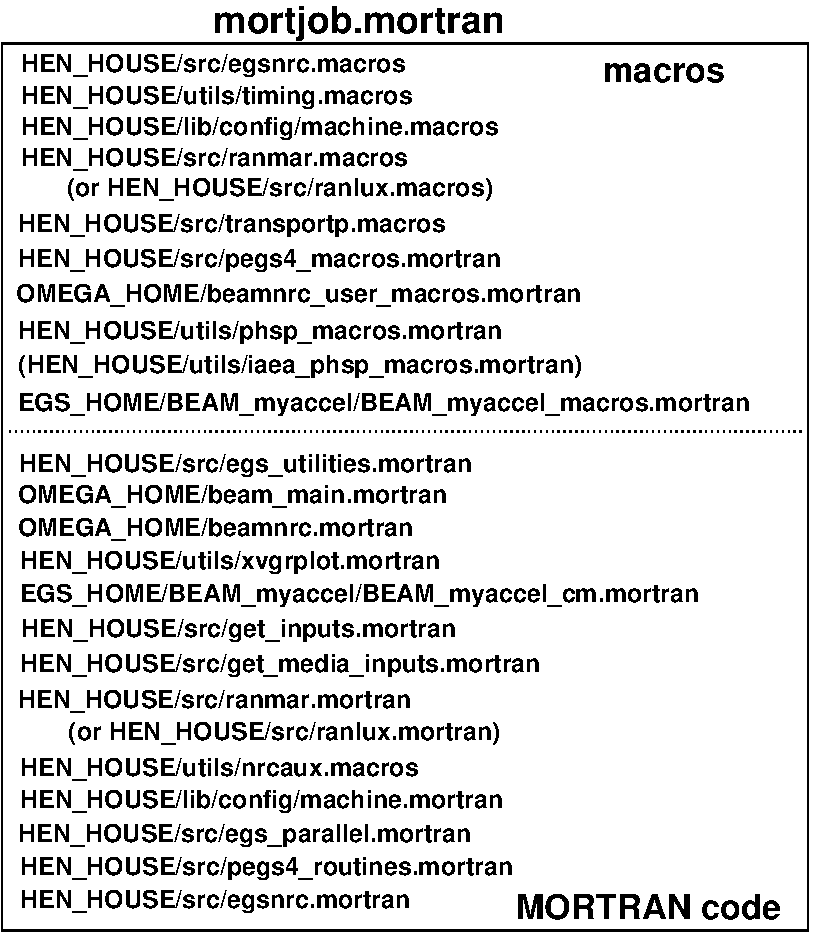
\includegraphics{figures/mortjob-mortran}
\caption[Files making up the complete BEAM source code.]
{Files concatenated to form the complete BEAM source code,
{\tt mortjob.mortran}, where {\tt BEAM\_myaccel\_cm.mortran}
and {\tt BEAM\_myaccel\_macros.mortran} contain
the source code related to all the selected CMs.  The files and
the order of concatenation are defined by the {\tt SOURCES} variable
in {\tt \$EGS\_HOME/BEAM\_myaccel/sources.make}.}
\label{fig_mortjob}
\end{center}
\end{figure}

A brief description of each of these files follows:
\begin{description}
\index{egsnrc.macros}
\item [{\tt egsnrc.macros}]  Macros for the EGSnrc system.  This
includes common blocks, such as {\tt STACK}, that are used by
all user codes.  See the EGSnrc Manual\cite{KR03} for more details.
\index{timing.macros}
\item [{\tt timing.macros}] Definitions of timing macros used in
BEAMnrc (and other user codes).  Replaces the macros with calls to
EGS subroutines used to determine elapsed CPU time, elapsed total
time, etc.
\index{\tt phsp\_macros.mortran}
\item[{\tt phsp\_macros.mortran}] Macros used by BEAMnrc to
read/write data from/to phase space files.  See section~\ref{PSF} for
more details.
\index{\tt iaea\_phsp\_macros.mortran}
\item[{\tt iaea\_phsp\_macros.mortran}] Macros used by BEAMnrc to
read/write phase space data in IAEA format.  This file is only present
if there is a working C++ compiler (required to compile the library of
IAEA phase space handling routines).  Otherwise, these macros are defined
as blank (``{\tt ;}'') in {\tt phsp\_macros.mortran} and IAEA-format phase
space data cannot be handled.
\index{machine.macros}
\item [{\tt machine.macros}] Machine/compiler-dependent macros.
Defines {\tt \$LONG\_INT} as {\tt integer*8} if it is available
on this machine, the record length factor ({\tt \$RECL-FACTOR}) for
a 4-byte record in a phase space file, etc.  See the EGSnrcMP Manual\cite{Ka03}
for more details.
\index{ranmar.macros}
\index{ranlux.macros}
\item [{\tt ranmar.macros} (or {\tt ranlux.macros})] Macros used by
BEAMnrc (and other user codes) to obtain random numbers, store random
number states to a file, retrieve random number states from a file and
initialize the random number generator.
\index{transportp.macros}
\item [{\tt transportp.macros}] Macros used by {\tt get\_inputs} to
define text patterns searched for in the EGSnrc input section of
a BEAMnrc input file (see section~\ref{egsnrc_inputs}).
\index{beamnrc\_user\_macros.mortran}
\item[{\tt beamnrc\_user\_macros.mortran}] Macros defining many
default BEAMnrc parameters such as the maximum number of dose/fluence
scoring zones, the maximum stack depth, etc.  These parameters often need to be
changed by the user.  See section~\ref{ctd} for more details.
\index{BEAM\_myaccel\_macros.mortran}
\item [{\tt BEAM\_myaccel\_macros.mortran}] Macros for all CMs that
comprise {\tt myaccel} concatenated together by {\tt beam\_build} with
the names of the CMs replaced by their identifiers as specified in
the {\tt myaccel.module} file.  See section~\ref{beambuildsect} for more details.
\index{egs\_utilities.mortran}
\item [{\tt egs\_utilities.mortran}]  Various EGSnrc utility codes.
Includes the {\tt egs\_init} functioning for initializing variable
arrays and opening any Fortran output units with the names given in
{\tt BEAM\_myaccel.io} (see section~\ref{iofilesect}).  Also includes
{\tt egs\_combine\_runs} routine for recombining results
after parallel runs (see section~\ref{recombinesect}).
\index{beam\_main.mortran}
\item [{\tt beam\_main.mortran}] BEAMnrc main code.  Consists
of calls to the main BEAMnrc subroutines,
{\tt beam\_init}, {\tt beam\_shower\_loop} and {\tt beam\_finish}
(in that order).  These subroutines are in {\tt beamnrc.mortran}
(see below).
\index{beam\_lib.mortran}
\item [{\tt beam\_lib.mortran}] Used instead of {\tt beam\_main.mortran}
when compiling BEAMnrc as a shared library for use as a source
(in DOSXYZnrc or other EGSnrc user code).  Contains macro (re)definitions
essential for use as a source along with subroutines for initializing
and sampling the BEAMnrc source.  Among these is a redefinition of the
\index{phase space writing macro}
main phase space writing macro which causes phase space data that would
normally be written to a phase space file to be stored in an array instead.
Incident particles for the simulation
using the BEAMnrc simulation as a source are then sampled from this array.
\index{beamnrc.mortran}
\item [{\tt beamnrc.mortran}] Contains definitions of macros used by
BEAMnrc, common blocks used by BEAMnrc and all BEAMnrc subroutines.
\index{xvgrplot.mortran}
\index{xmgr/xmgrace}
\item [{\tt xvgrplot.mortran}] Subroutine for creating a data file
suitable for plotting with xmgr/xmgrace.  BEAMnrc uses this
subroutine to output an {\tt .egsplot} file (see section~\ref{outputfilessect}).
\index{BEAM\_myaccel\_cm.mortran}
\item [{\tt BEAM\_myaccel\_cm.mortran}]  Subroutines for all
CMs comprising {\tt myaccel} concatenated together by {\tt beam\_build}
with CM names replaced by their identifiers as specified in
{\tt myaccel.module}.  See section~\ref{beambuildsect} for more details.
\index{get\_inputs.mortran}
\item [{\tt get\_inputs.mortran}] Coding for reading EGSnrc inputs from
the BEAMnrc input file.  See section~\ref{egsnrc_inputs} for more about these
inputs.
\index{ranmar.mortran}
\index{ranlux.mortran}
\item [{\tt ranmar.mortran} (or {\tt ranlux.mortran})] Subroutines used
by the RANMAR (or RANLUX) random number generator.  Many of the
macros defined in {\tt ranmar.macros} (or {\tt ranlux.macros}) include
calls to these subroutines.
\index{nrcaux.mortran}
\item [{\tt nrcaux.mortran}] Auxiliary MORTRAN routines used by
BEAMnrc (and other EGSnrc user codes).  Includes
\index{IWATCH}
\index{SUBROUTINE WATCH}
{\tt SUBROUTINE WATCH}, which outputs details of each
\index{.egsgeom file}
particle step/interaction or particle tracks to the {\tt .egsgeom} file
for display using EGS\_Windows, depending on the value of the
input variable {\tt IWATCH} (see section~\ref{iwatchsect} for more
on {\tt IWATCH}).
\index{machine.mortran}
\item [{\tt machine.mortran}]  Machine/configuration-dependent routines
such as date/time routines and system calls.  This file is created during
EGSnrcMP installation.  See the EGSnrc Users Manual\cite{KR03} and
EGSnrcMP Users Manual\cite{Ka03} for more info.
\index{egs\_parallel.mortran}
\item [{\tt egs\_parallel.mortran}] Subroutines for creating, opening,
reading from and writing to the job control ({\tt .lock}) file
during a parallel run (see section~\ref{parallelcalc}).
\index{egsnrc.mortran}
\item [{\tt egsnrc.mortran}] EGSnrc subroutines.  See the EGSnrc
Manual\cite{KR03} for more details.
\end{description}

Note that in previous versions of BEAMnrc, all of the BEAMnrc-specific
\index{beamnrc.mortran}
\index{beam\_main.mortran}
coding was contained in the file {\tt \$OMEGA\_HOME/beamnrc/beamnrc.mortran}.
Now, however, this coding has been broken up into two files: the
BEAMnrc main code is in \\{\tt \$OMEGA\_HOME/beamnrc/beam\_main.mortran}, and
the rest of the macro/subroutine definitions in
{\tt \$OMEGA\_HOME/beamnrc/beamnrc.mortran}.  Separating out the BEAMnrc
main code was necessary to allow us to compile BEAMnrc as a shared
library for use as a source in DOSXYZnrc and other EGSnrc user codes,
since shared libraries do not use the BEAMnrc main code.
See section~\ref{sharedlibsect} (page~\pageref{sharedlibsect}) for more
information about BEAMnrc as a shared library.

\section{Description of main BEAMnrc input file}
\label{dmbif}
\index{.egsinp}
The first section of an input file (\verb+.egsinp+) for BEAMnrc concerns
all issues not related to individual \verb+CMs+.  The following is taken
from the source code. More detailed discussion of most of these options
is given in the following sections (use the Index to find where in most
cases), but this is included here as a short summary/reference. Note that
the graphical user interface ({\tt BEAMnrc\_GUI}) greatly
simplifies the task of creating input files\cite{TR99} and the help files
in the GUI mostly duplicate what is below.
\index{BEAMnrc GUI} \index{GUI}
\index{input file!for main}

\begin{small}
\input{./inputformats/BEAM0.inp}
%\newline
\index{IWATCH} \index{ISTORE} \index{IRESTART} \index{IO\_OPT}
\index{IDAT} \index{LATCH!LATCH\_OPTION} \index{IZLAST}
\index{.egsgph}
\input{./inputformats/BEAM1.inp}
%\newline
\index{NCASE} \index{IXXIN,JXXIN} \index{TIMMAX} \index{IBRSPL}
\index{random number generator}
\index{NBRSPL} \index{IRRLTT}
\index{ICM\_SPLIT} \index{FS} \index{SSD} \index{NMIN}
\index{NSPLIT\_PHOT} \index{NSPLIT\_ELEC}
\index{ICM\_DBS}
\index{ZPLANE\_DBS}
\index{IRAD\_DBS}
\index{ZRR\_DBS}
\input{./inputformats/BEAM2.inp}
%\newline
\index{source!0 parallel circular beam}
\index{IQIN} \index{ISOURC} \index{RBEAM} \index{UINC}
\index{VINC} \index{WINC}
\input{./inputformats/BEAM3.inp}
%\newline
\index{source!1 point source}
\index{IQIN} \index{ISOURC} \index{RBEAM} \index{DISTZ} \index{GAMMA}
\index{XINL} \index{XINU} \index{YINL} \index{YINU}
\input{./inputformats/BEAM4.inp}
%\newline
\index{source!3 interior isotropic cylindrical source}
\index{IQIN} \index{ISOURC} \index{RMINBM} \index{RBEAM}
\index{ZSMIN} \index{ZSMAX}
\input{./inputformats/BEAM5.inp}
%\newline
\index{source!5 NRC swept beam}
\index{IQIN} \index{ISOURC} \index{RBEAM} \index{GAMMA}
\input{./inputformats/BEAM6.inp}
%\newline
\index{source!6 parallel rectangular beam}
\index{IQIN} \index{ISOURC} \index{XBEAM0} \index{YBEAM0}
\index{XBEAM} \index{YBEAM}
\input{./inputformats/BEAM7.inp}
%\newline
\index{source!7 scanning beam}
\index{IQIN} \index{ISOURC} \index{FD\_AT100} \index{IRATIO\_YXF}
\index{RBEAM}
\input{./inputformats/BEAM8.inp}
%\newline
\index{source!8 scanned point source for MM50:\\ uniform field coverage}
\index{IQIN} \index{ISOURC} \index{RBEAM} \index{DISTZ}
\input{./inputformats/BEAM9.inp}
%\newline
\index{source!9 scanned point source for MM50:\\ discrete field coverage}
\index{IQIN} \index{ISOURC} \index{DISTZ} \index{NPTS\_SRC9}
\index{X\_SRC9} \index{Y\_SRC9} \index{PROB\_SRC9}
\input{./inputformats/BEAM10.inp}
%\newline
\index{source!10 side parallel circular beam}
\index{IQIN} \index{ISOURC} \index{RBEAM} \index{UINC}
\index{VINC} \index{WINC}
\input{./inputformats/BEAM11.inp}
%\newline
\index{source!13 side parallel rectangular beam}
\index{IQIN} \index{ISOURC} \index{YBEAM} \index{ZBEAM}
\index{UINC} \index{VINC}
\input{./inputformats/BEAM12.inp}
%\newline
\index{source!15 NRC swept beam with radial distribution and divergence}
\index{IQIN} \index{ISOURC} \index{GAMMA} \index{ZFOCUS}
\index{RTHETAIN} \index{THETAIN}
\input{./inputformats/BEAM21.inp}
%\newline
\index{source!19 elliptical beam with Gaussian X-Y}
\index{IQIN} \index{ISOURC} \index{RBEAM} \index{UINC}
\index{VINC} \index{WINC}
\input{./inputformats/BEAM23.inp}
%\newline
\index{source!21 phase space}
\index{IQIN} \index{ISOURC} \index{INIT\_ICM} \index{SPCNAM}
\index{NRCYCL} \index{IPARALLEL}\index{PARNUM}
\index{ISRC\_DBS} \index{RSCR\_DBS} \index{SSDSRC\_DBS} \index{ZSRC\_DBS}
\input{./inputformats/BEAM13.inp}
\index{NRCYCL} \index{IPARALLEL}\index{PARNUM}
\index{ISRC\_DBS} \index{RSCR\_DBS} \index{SSDSRC\_DBS} \index{ZSRC\_DBS}
%\newline
\index{source!23 simulation source from user-specified angle}
\index{IQIN} \index{ISOURC} \index{INIT\_ICM} \index{ISRC\_DBS}
\index{ALPHA24} \index{BETA24} \index{DIST24}
\index{the\_beam\_code} \index{the\_pegs\_file}\index{the\_input\_file}
\input{./inputformats/BEAM33.inp}
%\newline
\index{source!24 phase space from user-specified angle}
\index{ALPHA24} \index{BETA24} \index{DIST24}
\input{./inputformats/BEAM34.inp}
%\newline
\index{beam characterization model}
\index{source!31 beam characterization model}
\index{IQIN} \index{ISOURC} \index{CMSOU} \index{SPCNAM}
\input{./inputformats/BEAM14.inp}
%\newline
\index{MONOEN} \index{EIN} \index{FILNAM} \index{NENSRC} \index{ENMIN}
\index{IMODE} \index{ENSRCD} \index{SRCPDF} \index{IOUTSP}
\input{./inputformats/BEAM15.inp}
%\newline
\index{ESTEPE} \index{SMAX} \index{ECUTIN} \index{PCUTIN} \index{IDORAY}
\index{IREJCT\_GLOBAL} \index{ESAVE!ESAVE\_GLOBAL} \index{IFLUOR}
\index{fluorescence} \index{range rejection}\index{PRESTA}
\index{IZ} \index{IREGLO} \index{IREGHI}
\input{./inputformats/BEAM16.inp}
%%%\newline
\index{IFORCE} \index{NFMIN} \index{NFMAX} \index{NFCMIN} \index{NFCMAX}
\index{forcing} \index{photon forcing}
\input{./inputformats/BEAM17.inp}
%\newline
\index{scoring plane!inputs}
\index{scoring zone!inputs}
\index{NSC\_PLANES} \index{IPLANE\_to\_CM} \index{NSC\_ZONES}
\index{scoring zone!type} \index{scoring zone!dimensions}
\index{MZONE\_TYPE} \index{RSCORE\_ZONE}
\index{XMIN\_ZONE}
\index{XMAX\_ZONE}
\index{YMIN\_ZONE}
\index{YMAX\_ZONE}
\index{NX\_ZONE}
\index{NY\_ZONE}
\index{grid scoring}
\index{scoring plane!ring scoring}
\index{scoring plane!grid scoring}
\input{./inputformats/BEAM18.inp}
%\newline
\index{contaminant dose!inputs}
\index{ITDOSE\_ON} \index{ICM\_CONTAM} \index{IQ\_CONTAM}
\index{LATCH!LATCH\_OPTION}
\index{LNEXC} \index{L\_N\_EXC} \index{LNINC} \index{L\_N\_INC}
\index{bit filters}
\index{dose components}
\input{./inputformats/BEAM19.inp}
%\newline
\index{Z\_min\_CM}\index{front of model}
\index{RMAX\_CM}
\input{./inputformats/BEAM20.inp}
\index{EGSnrc inputs}
\input{./inputformats/BEAM24.inp}
\index{Global ECUT}
\index{ECUT}
\index{ECUTIN}
\index{Global PCUT}
\index{PCUT}
\index{PCUTIN}
\index{Global SMAX}
\index{SMAX}
\index{SMAXIR}
\input{./inputformats/BEAM25.inp}
\index{ESTEPE}
\index{XIMAX}
\index{boundary crossing algorithm}
\index{bca\_algorithm}
\index{skin depth for BCA}
\index{skindepth\_for\_bca}
\input{./inputformats/BEAM26.inp}
\index{electron step algorithm}
\index{transport\_algorithm}
\index{spin effects}
\index{spin\_effects}
\index{bremsstrahlung angular sampling}
\index{IBRDST}
\index{bremsstrahlung cross sections}
\index{IBR\_NIST}
\index{bound Compton scattering}
\index{IBCMP}
\index{Compton cross sections}
\index{comp\_xsections}
\index{radiative Compton corrections}
\index{radc\_flag}
\input{./inputformats/BEAM27.inp}
\index{pair angular sampling}
\index{IPRDST}
\index{pair cross sections}
\index{pair\_nrc}
\index{photoelectron angular sampling}
\index{IPHTER}
\index{Rayleigh scattering}
\index{IRAYLR}
\index{atomic relaxations}
\index{IEDGFL}
\input{./inputformats/BEAM28.inp}
\index{electron impact ionization}
\index{eii\_flag}
\index{photon cross-sections}
\index{photon\_xsections}
\index{photon cross-sections!EPDL}
\index{photon cross-sections!XCOM}
\index{photon cross-sections!Storm-Israel}
\index{photon cross-sections output}
\index{xsec\_out}
\input{./inputformats/BEAM29.inp}
\index{rejection plane inputs}
\index{USE\_REJPLN}
\index{Z\_REJPLN}
\input{./inputformats/BEAM30.inp}
\index{bremsstrahlung cross section enhancement (BCSE) inputs}
\index{USE\_BCSE}
\index{MED\_BCSE}
\index{BCSE\_FACTOR}
\index{IRRLTT}
\input{./inputformats/BEAM31.inp}
\index{custom user inputs}
\index{PHSP\_OUTDIR}
\index{phase space files!redefining output directory}
\input{./inputformats/BEAM32.inp}
\index{EGSnrc inputs}
%\newline
\end{small}

\subsection{Sample input files}
\index{input file} \index{sample input files}
\index{example!test\_BEAMnrc}
\index{test\_BEAMnrc}
\index{script!test\_BEAMnrc}

\index{example!BEAMnrc input files}
Complete input files for simulation of a 10 MeV electron beam and a 16 MV
photon beam can be found in the appropriate subdirectories of:\\
\verb+$OMEGA_HOME/beamnrc/BEAMnrc_examples+
in files \verb+EX10MeVe.egsinp+ and \verb+EX16MVp.egsinp+
respectively. The file \verb+EXphantom.egsinp+ gives an example
of using BEAMnrc to do an efficient depth-dose calculation (but only for
the central axis).  These examples are described in
separate reports\cite{SR95,ZR95,WR95} which are somewhat dated since one
should now use the GUIs to run these examples.

\index{BEAMnrc\_examples}
The auxiliary script \verb+test_BEAMnrc+ (found on {\tt
\$HEN\_HOUSE/scripts})
automatically create the needed subdirectories on the user's area ({\tt
BEAM\_EX10MeVe} \etc) and
copy the relevant files to them so that the user may execute BEAMnrc
immediately (but the script only works on Linux/Unix and there is
no corresponding replacement for Windows).
\index{test\_BEAMnrc}
\clearpage
\section{Source Routines}

\index{source!general remarks}
In general, the incident particles move in the direction of the z-axis.  With
the exception of ISOURC=3 (internal isotropic source), =10 and 13 (x-ray
tube sources)  or =21 and 31 (phase space
inputs), the particles start being transported on the \verb+Z_min_CM(1)+
plane.  Conceptually, some of them originate at a point outside the accelerator
model and are essentially transported through vacuum to the accelerator
which starts at the \verb+Z_min_CM(1)+ plane.

\index{phase space files!as input}
One of the major features of BEAMnrc is that a
phase space file can be used as a source file between
any two  \verb+CMs+ in the accelerator. By writing a suitable off-line routine
to generate the appropriate phase space file
(use the macros in {\tt phsp\_macros.mortran}),
virtually any source can be simulated.  This feature also allows the accelerator
simulation to be broken up into components. For example, one might
simulate the fixed components at the top of an accelerator and then feed
the phase space file into a variety of calculations with different jaw
or applicator settings.
\index{phsp\_macros.mortran}\index{source routines!general}

For historic  and compatibility reasons, the input to specify the source type and the
charge of the incident beam are on a single line (as outlined in
section~\ref{dmbif}).  In particular, note that the first variable is
the charge, \verb+IQIN+,
or a dummy in those cases where the charge is determined
elsewhere (\eg\ for a phase space file input).
\index{IQIN}

The following subsections describe the source routines available in BEAMnrc.


\begin{description}

\item [ISOURC=0] Parallel Circular Beam
\item [ISOURC=1] Isotropic Point Source on Z-axis
\item [ISOURC=3] Interior Isotropic Cylindrical Source
\item [ISOURC=5] NRC Swept Beam
\item [ISOURC=6] Parallel Rectangular Beam
\item [ISOURC=7] Scanning Beam (sawtooth)
\item [ISOURC=8] Scanning Point Source for MM50
\item [ISOURC=9] Discrete Point Source for MM50
\item [ISOURC=10] Parallel Circular Beam Incident from Side
\item [ISOURC=13] Parallel Rectangular Beam Incident from Side
\item [ISOURC=15] NRC Swept Beam with Radial Intensity Distribution and
                  Radial Divergence
\item [ISOURC=19] Elliptical Beam with Gaussian Distributions in X and Y,
                  Parallel or with Radial Divergence
\item [ISOURC=21] Phase Space Source
\item [ISOURC=23] BEAMnrc Simulation Source
\item [ISOURC=24] Phase Space Source Incident from User-specified Angle
\item [ISOURC=31] Beam characterization Model

\end{description}

\subsection{ISOURC=0: Parallel Circular Beam}
\cen{IQIN, 0, RBEAM, UINC, VINC, WINC}
\index{UINC} \index{VINC} \index{WINC}
\index{RBEAM}\index{Z\_min\_CM}
\index{source!0 parallel circular beam}

The parallel circular beam is always assumed to be incident on the
center of the front
of the first CM (\ie\ at \verb+Z_min_CM(1)+).  The input parameters are:
\begin{description}
\item [IQIN] The charge of the incident beam (defaults to 0=photons)
\item [RBEAM] Radius of the beam in cm (maximum is \verb+RMAX_CM(1)+
 for a circular first CM or
$\sqrt{2}$\verb+RMAX_CM(1)+ for a square first CM,
it defaults to maximum if set $>$
maximum)
\item [UINC] X-axis direction cosine (defaults to 0)
\item [VINC] Y-axis direction cosine (defaults to 0)
\item [WINC] Z-axis direction cosine (defaults to 1, \ie\ parallel to
the z-axis)
\end{description}
UINC, VINC, and WINC are automatically normalized by
(UINC$^2$+VINC$^2$+WINC$^2$).
Note that it is possible to have \verb+RBEAM+ = 0; this is a pencil beam.
Figure~\ref{fig_src0} below shows the parallel circular beam and its input parameters.
\begin{figure}[htbp]
\begin{center}
\htmlimage{scale=2.0}
\leavevmode
\mbox{}\hspace{0cm}
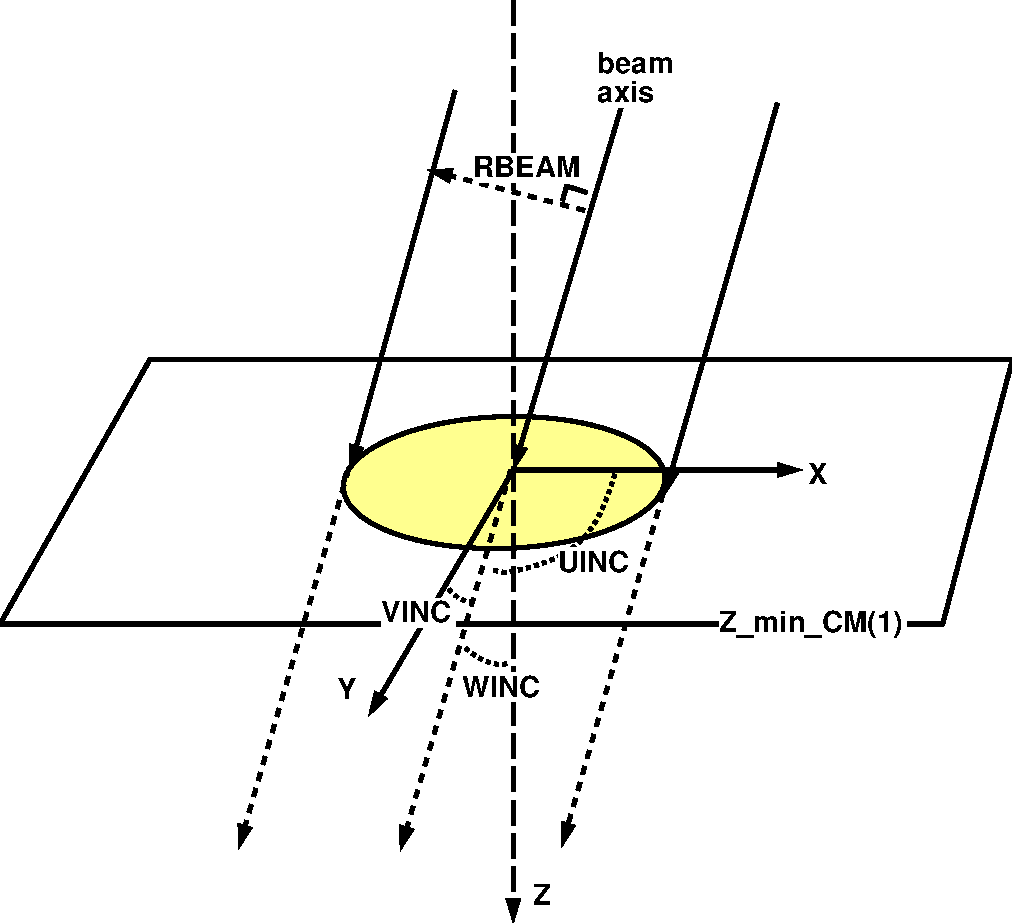
\includegraphics[height=8.5cm]{figures/src0}
\caption[ISOURC=0: Parallel circular beam.]
{Parallel Circular Beam (ISOURC=0) showing the beam radius,
{\tt RBEAM}, and the
direction cosines, UINC, VINC and WINC.  Note that {\tt RBEAM} is measured perpendicular
to the beam central axis.  The beam axis always intersects {\tt Z\_min\_CM(1)}
 at (X=0,Y=0).}
\label{fig_src0}
\end{center}
\end{figure}

%\setlength{\textheight}{10.0in}
\clearpage
\vspace*{-2cm}
\subsection{ISOURC=1: Isotropic Point Source on Z-axis}
\vspace*{-0.2cm}
\cen{IQIN, 1, DISTZ, RBEAM, GAMMA, XINL, XINU, YINL, YINU}
\index{GAMMA}
\index{DISTZ}
\index{RBEAM}
\index{XINL}\index{XINU}\index{YINL}\index{YINU}
\index{source!1 point source}

The isotropic point source is placed on the Z-axis.  It is
assumed to be incident on the first CM, but can be placed any distance above
\verb+Z_min_CM(1)+.  The beam field can be circular or
rectangular (see below).
The circular beam is centred on the Z axis, while the rectangular beam can
be placed anywhere on the top surface of CM 1.
\begin{description}
\item [DISTZ] Distance of the source above \verb+Z_min_CM(1)+ in cm (defaults to 100 cm)
\item [RBEAM] Radius of circular field at \verb+Z_min_CM(1)+ (if $>$ 0).
If {\tt RBEAM}=0, then {\tt GAMMA} (see below) is used to define the
circular field.  If {\tt RBEAM}$<$0, then
{\tt XINL}, {\tt XINU}, {\tt YINL}, {\tt YINU} (see below) are used to define a
rectangular field.  Maximum value of {\tt RBEAM} is
\verb+RMAX_CM(1)+ (circular CM 1) or $\sqrt{2}$\verb+RMAX_CM(1)+ (square CM 1).
{\tt RBEAM} defaults to maximum if it is set $>$ maximum or if
\verb+RBEAM+=0.0 and \verb+GAMMA+ = 0.0.
\item [GAMMA] Half-angle of circular field
at \verb+Z_min_CM(1)+ relative to the point source
(Note that this is simply another way of specifying the radius of a circular field,
and is only used if \verb+RBEAM+ = 0.0; defaults to give maximum radius [see
description of \verb+RBEAM+ above] if
it is set so that the radius would be $>$ maximum).
\item [XINL, XINU, YINL, YINU] Min. X, Max. X, Min. Y, Max Y dimensions
 of rectangular field (only used if {\tt RBEAM}$<$0) in cm.
The rectangular field
is restricted to -\verb+RMAX_CM(1)+$\leq$X$\leq$\verb+RMAX_CM(1)+ and
-\verb+RMAX_CM(1)+$\leq$Y$\leq$\verb+RMAX_CM(1)+.  The dimensions can be set
to give a line or point ``field'' anywhere on the top of CM 1.
\end{description}
\verb+DISTZ+, between the source and \verb+Z_min_CM(1)+ is assumed to be a vacuum.
Figure~\ref{fig_src1} below illustrates the point source and its input variables.
\begin{figure}[h]
\vspace*{-0.3cm}
\begin{center}
\leavevmode
\mbox{}\hspace{0cm}
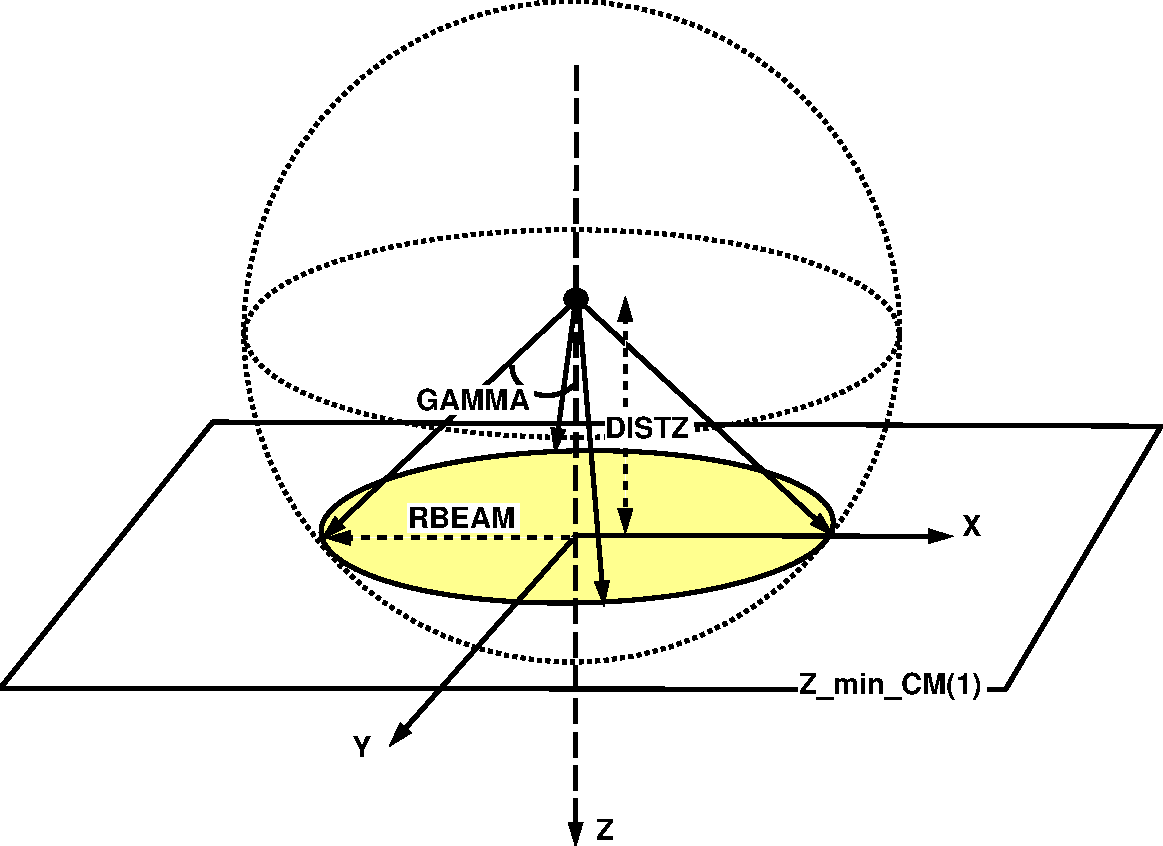
\includegraphics[height=7.5cm]{figures/src1}
\vspace*{-0.5cm}
\caption[ISOURC=1: Point isotropic source on Z-axis.]
{Point source (ISOURC=1) showing the distance of the source above
{\tt Z\_min\_CM(1)}, specified by {\tt DISTZ}, and the two different ways of
specifying a circular field at {\tt Z\_min\_CM(1)}, {\tt RBEAM}
and {\tt GAMMA}.  A rectangular
beam anywhere on the top surface of CM 1
can be specified by setting {\tt RBEAM}$<$0 and
using {\tt XINL}, {\tt XINU}, {\tt YINL}, {\tt YINU} to define the beam.}
\label{fig_src1}
\end{center}
\end{figure}

\clearpage
\subsection{ISOURC=3: Interior Isotropic Cylindrical Source}
\label{isourc3sect}
\cen{IQIN, 3, RMINBM, RBEAM, ZSMIN, ZSMAX}
\index{cylindrical source}
\index{RMINBM}
\index{RBEAM}
\index{ZSMIN}
\index{ZSMAX}
The uniform radiating cylindrical isotropic source can be a ring
centred on the Z-axis or a cylinder with its central axis parallel to
the X-axis.  The orientation is controlled by the sign of the input variable,
\verb+RBEAM+ (see below).  The source is contained within the geometry
of one or more component modules (\ie\ it is able to span adjacent CMs).
Currently, this source can only be used inside
\verb+CONESTAK, SIDETUBE or FLATFILT+ CMs because of the need to
identify the initial regions.
\typeout{*******ISOURC=3 interior   WHY ONLY CONESTAK***********initial regions}
\typeout{*******ISOURC=3 interior   what if OUTSIDE CM ********************}
The input parameters for this source are:
\begin{description}
\item [RMINBM] Inner radius of vertical ring (if \verb+RBEAM+ $\geq$ 0){\it
or} Z position of centre of horizontal cylinder (if \verb+RBEAM+ $<$ 0)
\item [RBEAM] Outer radius of vertical ring (if $\geq$ 0){\it or} negative
radius of horizontal cylinder (if $<$ 0) (for vertical ring,
maximum value is \verb+RMAX_CM+ of largest CM containing the source;
for horizontal cylinder, maximum value
keeps the radius entirely contained between \verb+Z_min_CM(1)+ and the
bottom of the geometry; defaults to maximum if absolute value is $>$ maximum)
\item [ZSMIN] Z of top of vertical ring (if \verb+RBEAM+ $\geq$ 0){\it
or} minimum X
of horizontal cylinder (if \verb+RBEAM+ $<$ 0) (for vertical ring, minimum
value is \verb+Z_min_CM(1)+; for horizontal cylinder, minimum is
\verb+-RMAX_CM+ of largest CM containing source; defaults to minimum if set $<$
minimum) \item [ZSMAX] Z of bottom of vertical ring (if \verb+RBEAM+ $\geq$ 0)
{\it or} maximum X of horizontal cylinder (if \verb+RBEAM+ $<$ 0) in cm (for vertical
ring, maximum is the bottom of geometry; for horizontal cylinder, maximum is
\verb+RMAX_CM+ of largest CM containing source; defaults to maximum if set $>$
maximum)
\end{description}
\begin{figure}[htbp]
\begin{center}
\htmlimage{scale=2.0}
\leavevmode
\vspace{-0.8cm}
\mbox{}\hspace{0cm}
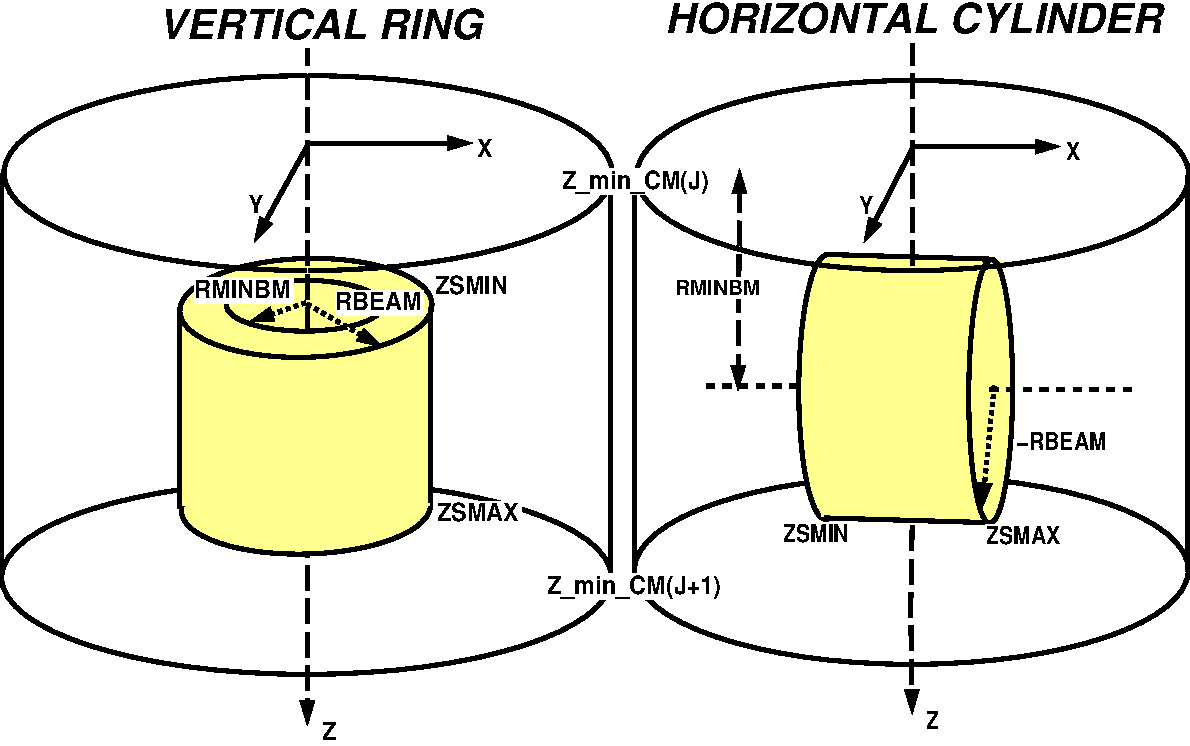
\includegraphics[height=6.0cm]{figures/src3}
\caption[ISOURC=3: Interior isotropic cylindrical source.]
{Uniform isotropic radiating source (ISOURC=3) which is interior to
the accelerator model.  For vertical ring
configuration shown on the left, set
{\tt RBEAM} $\geq$ 0.  For horizontal cylinder configuration on
right set {\tt RBEAM} $<$ 0.  The meaning of the
input variables depends on the configuration.  The
source is shown within a single CM, however it can span any number of
adjacent CMs.}
\label{fig_src3}
\end{center}
\end{figure}

\clearpage
\subsection{ISOURC=5: NRC Swept BEAM}
\cen{IQIN, 5, GAMMA, RBEAM}
\index{GAMMA}
\index{swept beam}
\index{RBEAM}
\index{source!5 NRC swept beam}
The NRC swept beam is a parallel circular beam
swept around the outside
of an imaginary cone.  The beam is assumed incident on the front of CM
1.  The apex of the imaginary cone is always at
(X=0,Y=0,Z=\verb+Z_min_CM(1)+), and the cone angle is variable.
Input parameters for this source are:
\begin{description}
\item [IQIN] Charge of the incident beam (defaults to 0 = photons)
\item [GAMMA] Half-angle of the cone in degrees (0$^o$ $\leq$ \verb+GAMMA+ $<$
90$^o$)
\item [RBEAM] Radius of the beam in cm (maximum value \verb+RMAX_CM(1)+
 if the
first CM
is circular or $\sqrt{2}$\verb+RMAX_CM(1)+
 if the first CM is square, defaults to
maximum if set $>$ maximum)
\end{description}
Figure~\ref{fig_src5} below shows the swept beam source and its input
parameters.
\begin{figure}[htbp]
\begin{center}
\htmlimage{scale=2.0}
\leavevmode
\mbox{}\hspace{0cm}
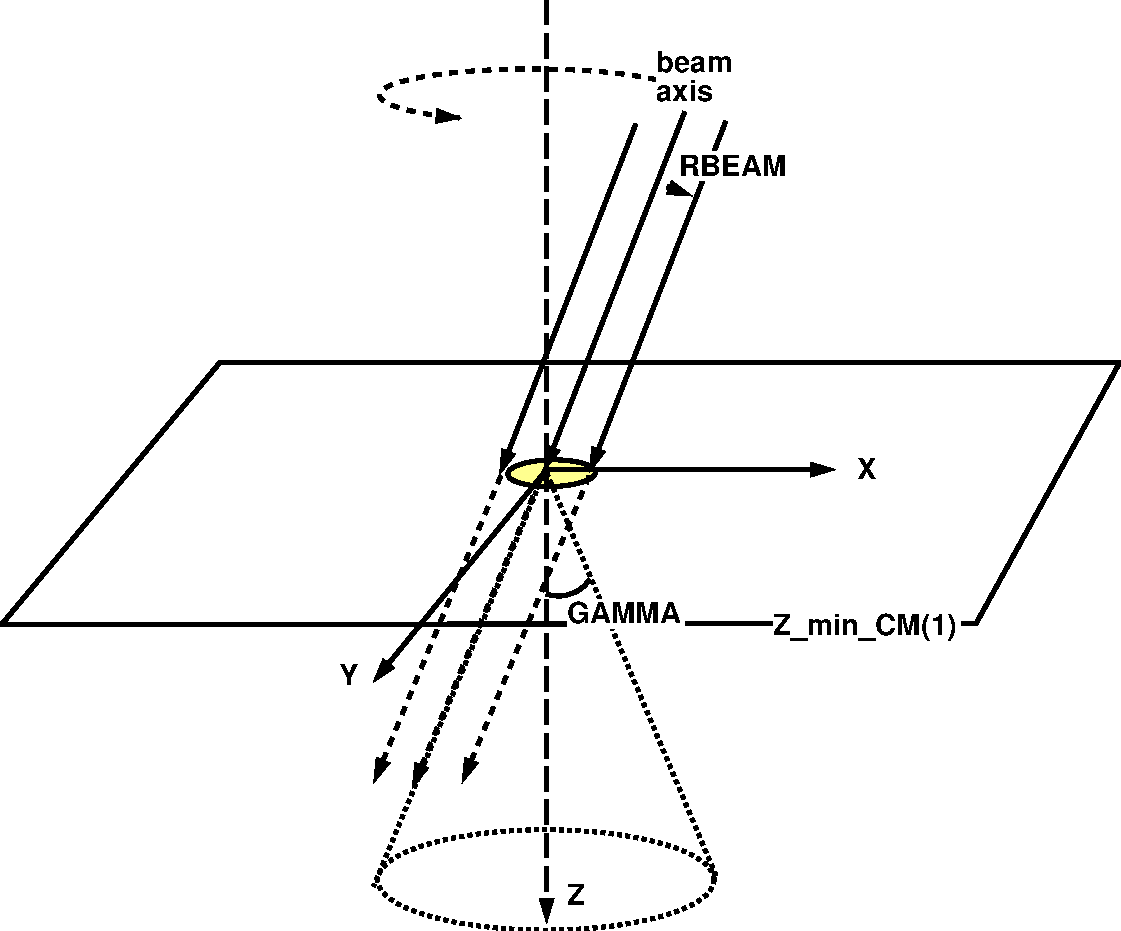
\includegraphics[height=10cm]{figures/src5}
\caption[ISOURC=5: NRC swept beam]
{NRC swept beam source (ISOURC=5) showing the incident beam, with radius
{\tt RBEAM},
sweeping the surface of an imaginary cone with apex half-angle {\tt GAMMA}.
Note that it is the beam axis which actually sweeps the surface of the
cone.}
\label{fig_src5}
\end{center}
\end{figure}

\clearpage
\subsection{ISOURC=6: Parallel Rectangular Beam}
\cen{IQIN, 6, XBEAM0, YBEAM0, XBEAM, YBEAM}
\index{XBEAM} \index{YBEAM}
\index{source!6 parallel rectangular beam}
The parallel rectangular beam is the rectangular equivalent of the
parallel circular beam (ISOURC=0) with the exception that the beam
cannot be oblique, it is always perpendicular to
the front surface of the first CM and this beam can be offset from the
Z-axis.
Input parameters for the parallel rectangular beam are:
\begin{description}
\item [IQIN] Charge of beam (defaults to 0 = photons)
\item [XBEAM0] X position of beam centre in cm (defaults to 0 if
\verb+XBEAM0+$^2$ + \verb+YBEAM0+$^2$ $>$ \verb+RMAX_CM(1)+$^2$ when
the first CM is circular
or if $|$\verb+XBEAM0+$|$ or $|$\verb+YBEAM0+$|$ $>$ \verb+RMAX_CM(1)+
 when the first CM is a square)
\item [YBEAM0] Y position of beam centre in cm (defaults to 0 under same
conditions as \verb+XBEAM0+)
\item [XBEAM] Half-width of beam in X-direction in cm (defaults to keep
$|$\verb+XBEAM0+$|$ + $|$\verb+XBEAM+$|$ $\leq$ \verb+RMAX_CM(1)+)

\item [YBEAM] Half-width of beam in Y-direction in cm (defaults to keep
$|$\verb+YBEAM0+$|$ + $|$\verb+YBEAM+$|$ $\leq$ \verb+RMAX_CM(1)+

\end{description}
\begin{figure}[hbp]
\htmlimage{scale=2.0}
\leavevmode
\begin{center}
\mbox{}\hspace{0cm}
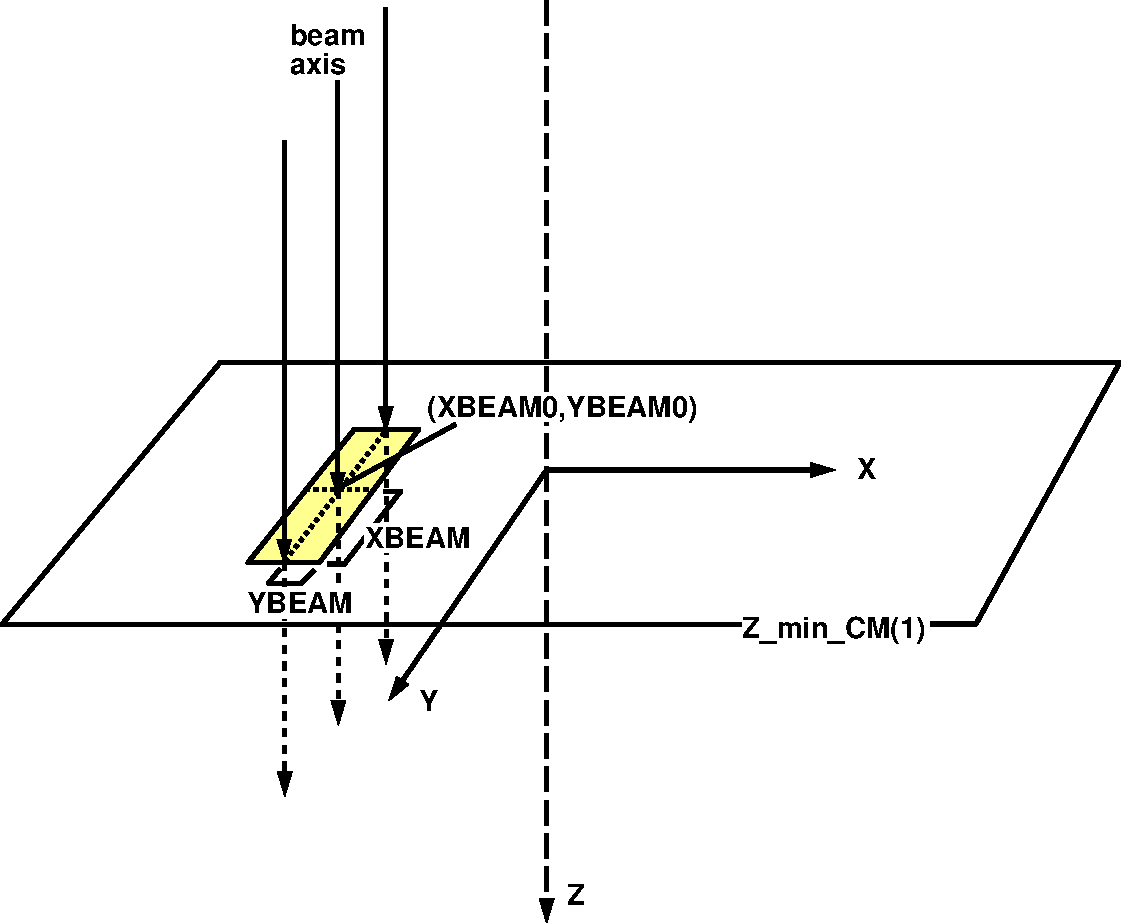
\includegraphics[height=8.6cm]{figures/src6}
\caption[ISOURC=6: Parallel rectangular beam.]
{Parallel rectangular beam (ISOURC=6) showing the beam centre
({\tt XBEAM0},{\tt YBEAM0}) and the X and Y half-widths
 ({\tt  XBEAM},{\tt YBEAM}).}
\label{fig_src6}
\end{center}
\end{figure}

\clearpage

\subsection{ISOURC=7: Scanning Sawtooth Beam}
\cen{IQIN, 7, FD\_AT100, IRATIO\_YXF, RBEAM}
\index{FD\_AT100} \index{IRATIO\_YXF}
\index{RBEAM}
\index{source!7 scanning sawtooth beam}

In the scanning sawtooth beam source, a circular parallel beam, incident on the
front of the first CM,
is scanned in a zig-zag pattern on the X-Y plane.   The angle for the
scan is selected as the particles leave the \verb+Z_min_CM(1)+ plane.
This is an approximation of the real case where the beam is bent below
this point usually.  The source randomly selects points in the scan.
The input parameters are:
\begin{description}
\item [IQIN] Charge of the incident beam (defaults to 0 = photons)
\item [FD\_AT100] Scanning field size at SSD=100cm in cm (field is
{\tt FD\_AT100} x {\tt FD\_AT100}). This is often much greater than the actual field
size.
\item [IRATIO\_YXF] The number of Y scans per X scan (defaults to 6.5 if
set $\leq$ 0; also, 2x{\tt IRATIO\_YXF} is always rounded up to the nearest odd
integer)
\item [RBEAM] Radius of the incident beam in cm (defaults to 0.01 cm if
set $\leq$ 0; defaults to maximum of \verb+RMAX_CM(1)+ [circular CM 1] or
$\sqrt{2}$\verb+RMAX_CM(1)+ [square CM 1] if set $>$ maximum)
\end{description}
Note that the field is always scanned twice in the X direction; thus,
the number of Y scans is 2x{\tt IRATIO\_YXF}.  It is also important to note
that {\tt FD\_AT100} defines the field size covered by the beam central axis;
a beam with finite \verb+RBEAM+ will actually go outside {\tt
FD\_AT100}.
Figure ~\ref{fig_src7} below shows the scanning beam and its various
input parameters.
\begin{figure}[htbp]
\htmlimage{scale=2.0}
\leavevmode
\begin{center}
\mbox{}\hspace{0cm}
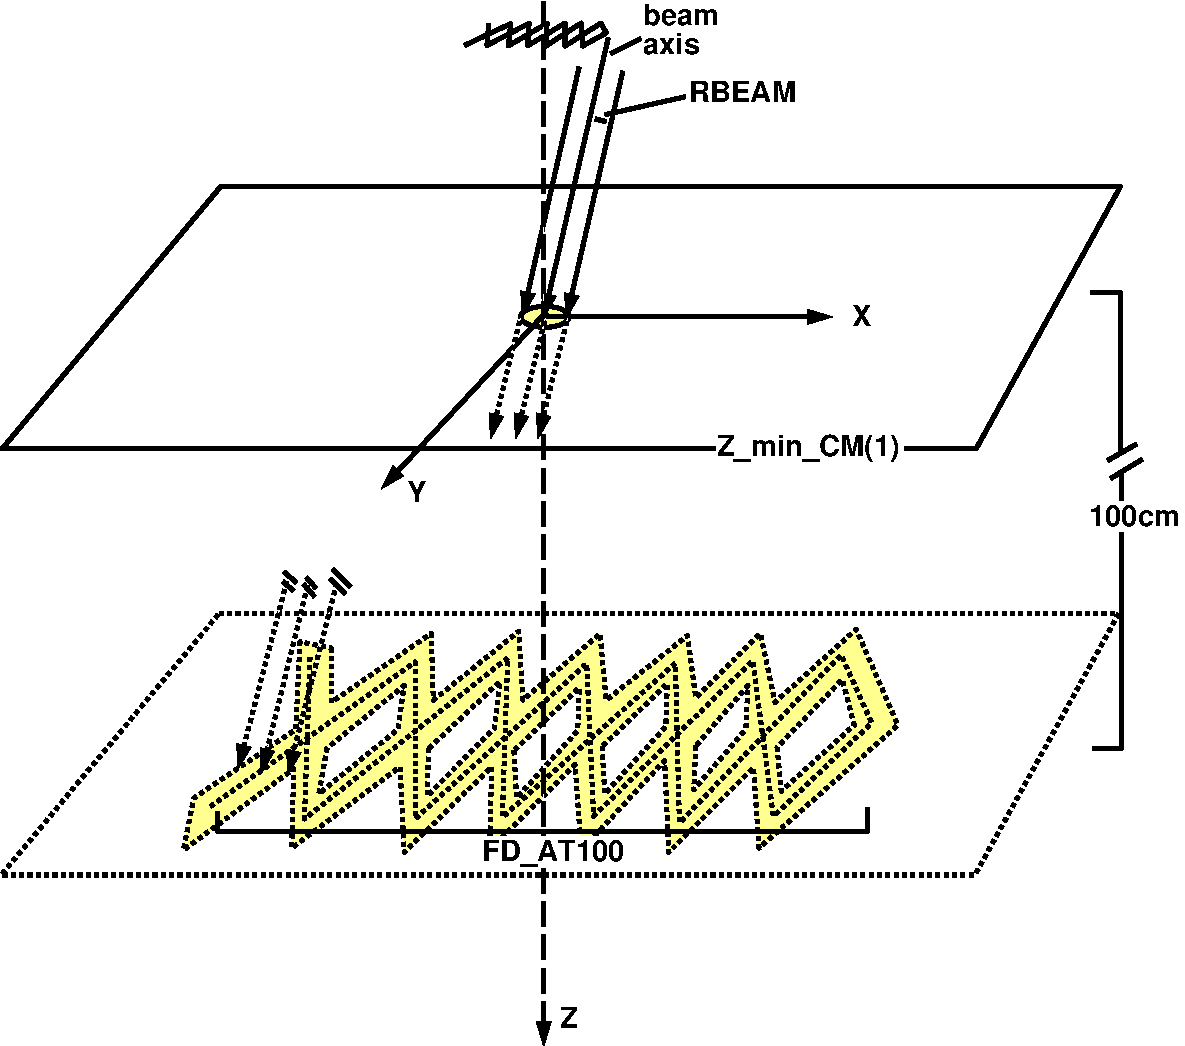
\includegraphics[height=8cm]{figures/src7}
\caption[ISOURC=7: Scanning sawtooth beam]
{Scanning beam (ISOURC=7).  The parallel circular beam of radius
{\tt RBEAM}
is scanned in a zig-zag pattern in the X-Y plane to produce the zig-zag
coverage at SSD=100cm.  In the case shown here, {\tt IRATIO\_YXF} = 6.5; hence
there are a total of 13 Y scans.}
\label{fig_src7}
\end{center}
\end{figure}

%\setlength{\textheight}{10.0in}
\clearpage
\subsection[ISOURC=8: Scanned Point Source for MM50--Uniform]{ISOURC=8: Scanned Point Source for MM50--Uniform Field}
\index{source!8 scanned point source for MM50:\\ uniform field }
\cen{IQIN, 8, DISTZ, RBEAM, RBEAM0}
\index{DISTZ}
\index{RBEAM}
\index{RBEAM0}

This source is designed to simulate the source used in the MM50 linear
accelerator for electron beams.
The source behaves like a point source
located at Z=0 scanned to produce a uniform distribution of particles at
a user-specified distance from the source ({\tt DISTZ}) over a field
of user-specified radius ({\tt RBEAM}).  Uncertainty in the X-Y position
of the source at Z=0 can be simulated using the beam spot radius, {\tt RBEAM0}.
If {\tt RBEAM0} $>$ 0,
the particle distribution at {\tt DISTZ}
will be uniform out to {\tt RBEAM} and tails off between
{\tt RBEAM} and {\tt RBEAM + RBEAM0}.
Note that \verb+Z_min_CM(1)+ must be $\geq$ 0 for this source.
Input parameters are:
\begin{description}
\index{IQIN}
\item [IQIN] Charge of the incident beam (defaults to 0 = photon)
\item [DISTZ] The source-to-surface distance (SSD) at which uniform
particle distribution is desired in cm (defaults to 100 cm if it is set $\leq$ 0)
\item [RBEAM] Radius of the field at \verb+DISTZ+ in cm (defaults to maximum
value of \\
{\tt RMAX\_CM(1)*DISTZ/Z\_min\_CM(1)} for circular CM 1 or
$\sqrt{2}${\tt RMAX\_CM(1)*DISTZ/Z\_min\_CM(1)} for square CM 1)
\item [RBEAM0] Radius of the beam spot at Z=0 in cm (defaults to 0 if
set $<$ 0 and gets reset to
max. value of {\tt RBEAM} - {\tt RBEAM} if
{\tt RBEAM+RBEAM0} $>$ max. value of {\tt RBEAM})
\end{description}
\vspace*{-0.5cm}
\begin{figure}[htbp]
\begin{center}
\htmlimage{notransparent}
\leavevmode
\mbox{}\hspace{0cm}
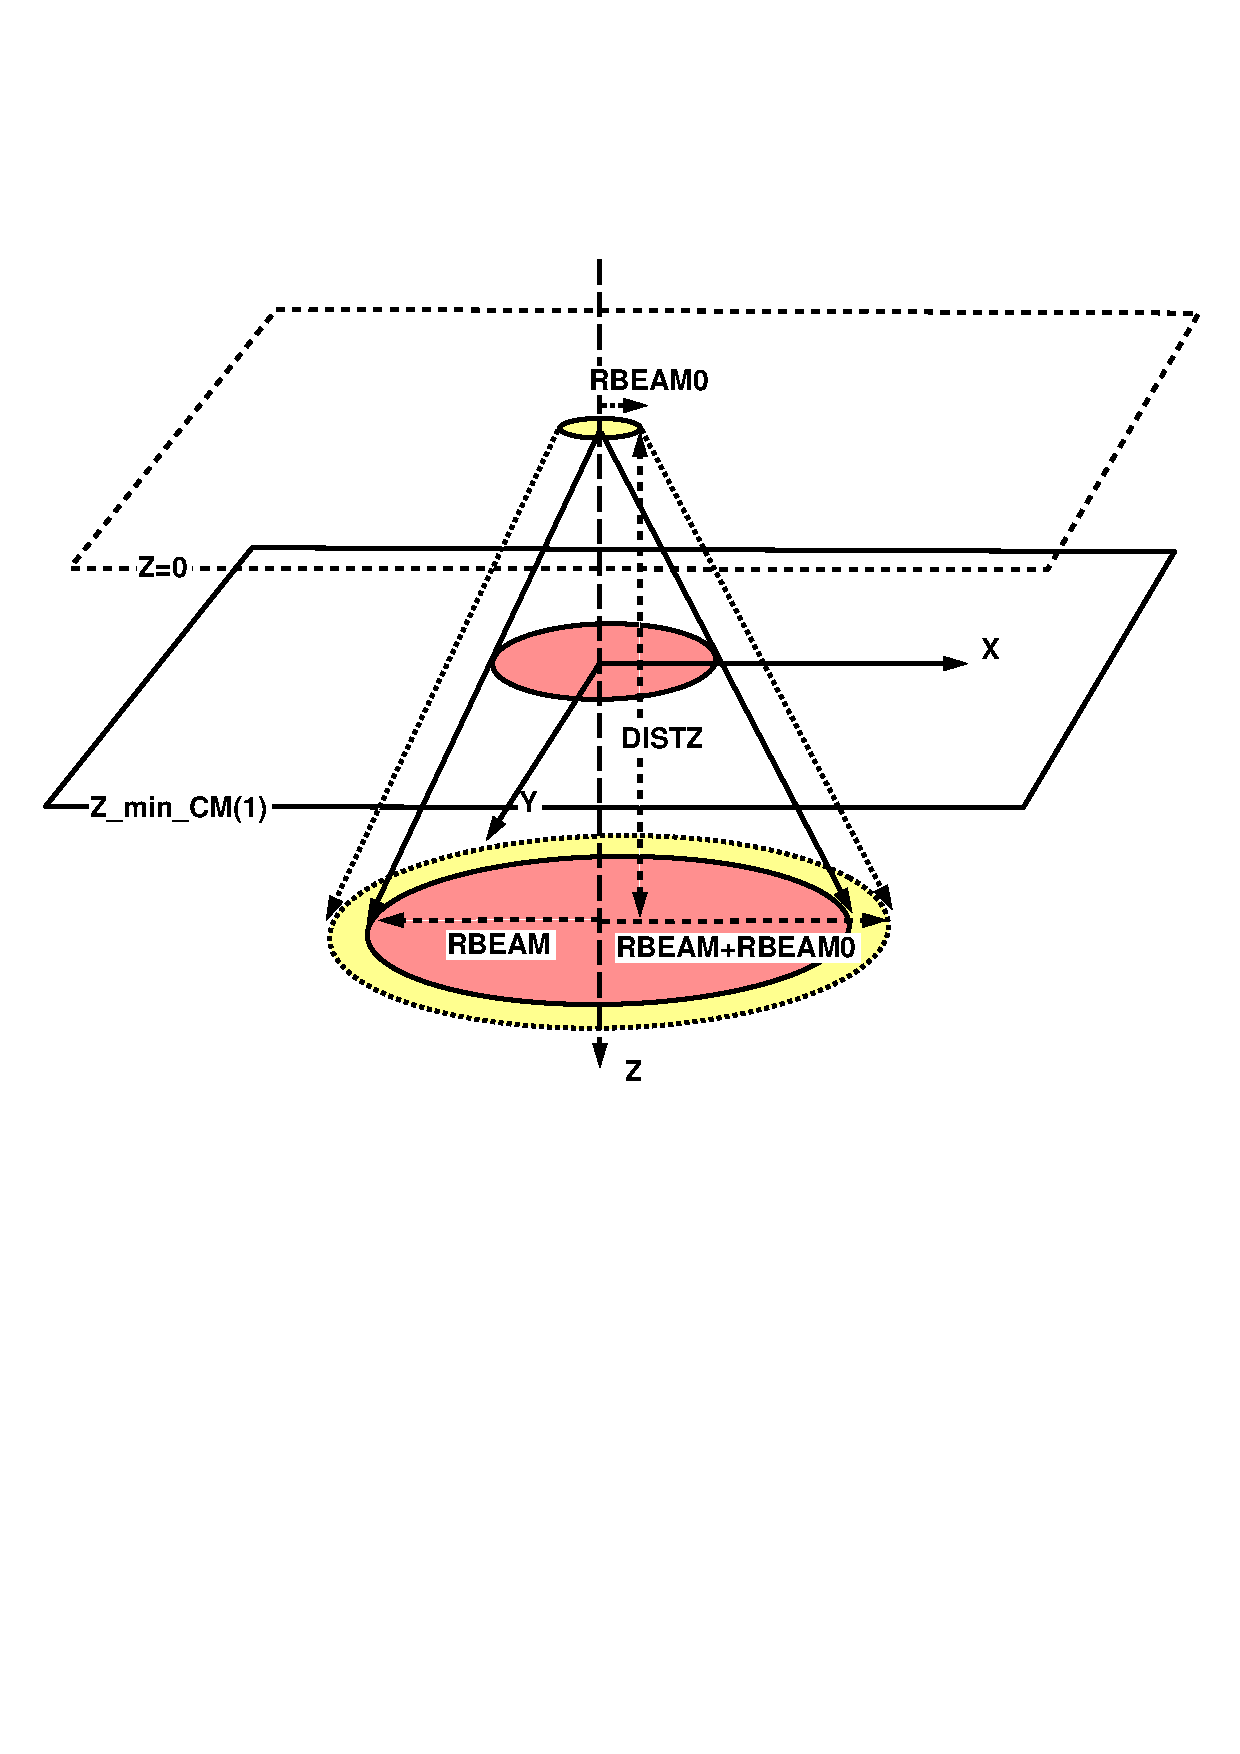
\includegraphics[height=8cm]{figures/src8}
\caption[ISOURC=8: Scanned circular uniform source.]
{Scanned point source producing uniform field coverage (ISOURC=8).  The figure
shows a point source at
Z=0 scanned to give uniform particle distribution in a field of radius
{\tt RBEAM} at a distance {\tt DISTZ} below the source.  The uncertainty
of the position of the source at Z=0, is simulated using {\tt RBEAM0}.
Particles can originate anywhere within the circle defined by {\tt RBEAM0}
which results in a particle distribution at {\tt DISTZ} which is uniform
out to {\tt RBEAM} and falls off between {\tt RBEAM} and {\tt RBEAM+RBEAM0}.}
\label{fig_src8}
\end{center}
\end{figure}

\clearpage

\subsection[ISOURC=9: Scanned Point Source for MM50--Discrete]{ISOURC=9: Scanned Point Source for MM50--Discrete Field}
\index{source!9 scanned point source for MM50: \\discrete field}
\cen{IQIN, 9, DISTZ, NPTS\_SRC9 \\
X\_SRC9, Y\_SRC9, PROB\_SRC9}
\index{DISTZ}
\index{NPTS\_SRC9}
\index{X\_SRC9}
\index{Y\_SRC9}
\index{PROB\_SRC9}

This source is designed to simulate the source used in the MM50 linear
accelerator to produce photon beams.  It behaves like a point source emanating
pencil beams to a finite number of dwell points, providing
discrete field coverage.  The user specifies by the X,Y coordinates
of the dwell points on a plane perpendicular to the Z-axis at
a user-specified source-to-surface distance (SSD) and the
probability of a particle being initially directed towards each point.
The source is always considered to be at Z=0.
Input parameters are:
\begin{description}
\item [IQIN] Charge of the incident beam (defaults to 0 = photon)
\item [DISTZ] The source-to-surface distance (SSD) in cm
(defaults to 100 cm if it is set $\leq$ 0)
\item [NPTS\_SRC9] The number of points used to cover the
field (defaults to 1 if set $\leq$ 0)
\item [X\_SRC9(I) (I=1,...,NPTS\_SRC9)] The X coordinate of
point I on plane $\perp$ Z at \verb+DISTZ+ in cm
\item [Y\_SRC9(I) (I=1,...,NPTS\_SRC9)] The Y coordinate of
point I on plane $\perp$ Z at \verb+DISTZ+ in cm
\item [PROB\_SRC9(I) (I=1,...,NPTS\_SRC9)] The probability of a particle
being incident\\ on point I.  Probabilities are automatically
normalized.
\end{description}
\begin{figure}[htbp]
\begin{center}
\leavevmode
\mbox{}\hspace{0cm}
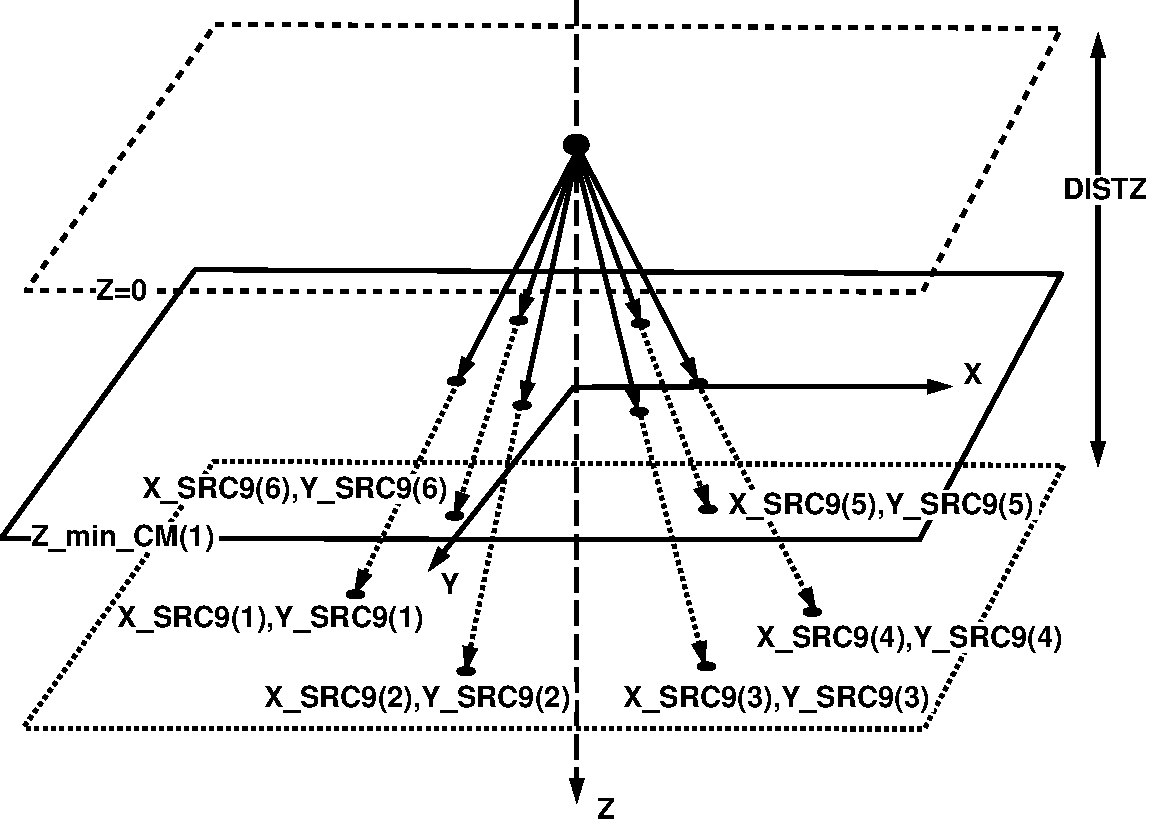
\includegraphics[height=7cm]{figures/src9}
\caption[ISOURC=9: Discrete beams from point source.]
{Scanned point source for discrete field coverage (ISOURC=9).
The figure shows a point source at Z=0 producing 6 points scattered over
the field ({\tt NPTS\_SRC9}=6).  The user specifies the source-to-surface
distance, {\tt DISTZ}, the X and Y coordinates of the points at {\tt DISTZ},
{\tt (X\_SRC9(I),Y\_SRC9(I))}, and the probability of a particle being
incident at each point, {\tt PROB\_SRC9(I)} (not shown).  }
\label{fig_src9}
\end{center}
\end{figure}

%\setlength{\textheight}{9.0in}
\clearpage

\subsection{ISOURC=10: Parallel Circular Beam Incident from Side}
\cen{IQIN, 10, RBEAM, UINC, VINC, WINC}
\index{UINC} \index{VINC} \index{WINC}
\index{RBEAM}
\index{source!10 side parallel circular beam}

This parallel circular beam enters the first CM from the side and can only
be used as the source for an XTUBE.
The input parameters for this source are:
\begin{description}
\item [IQIN] Charge of incident beam (defaults to 0 = photons)
\item [RBEAM] Radius of beam in cm (defaults to half the thickness of the
first CM
if it is greater than this and to 0 if it is set $<$ 0)
\item [UINC] Incident X-axis direction cosine (should be $<$ 0 so the beam
faces the Z-axis; reset to -UINC if it is $>$ 0)
\item [VINC] Incident Y-axis direction cosine
\item [WINC] Incident Z-axis direction cosine\\
(UINC, VINC, WINC default to -1,0,0 if UINC$^2$+VINC$^2$+WINC$^2$ = 0)
\end{description}
The direction cosines UINC, VINC and WINC are each automatically
normalized by\\
(UINC$^2$+VINC$^2$+WINC$^2$).
\begin{figure}[htbp]
\begin{center}
\htmlimage{scale=2.0}
\leavevmode
\mbox{}\hspace{0cm}
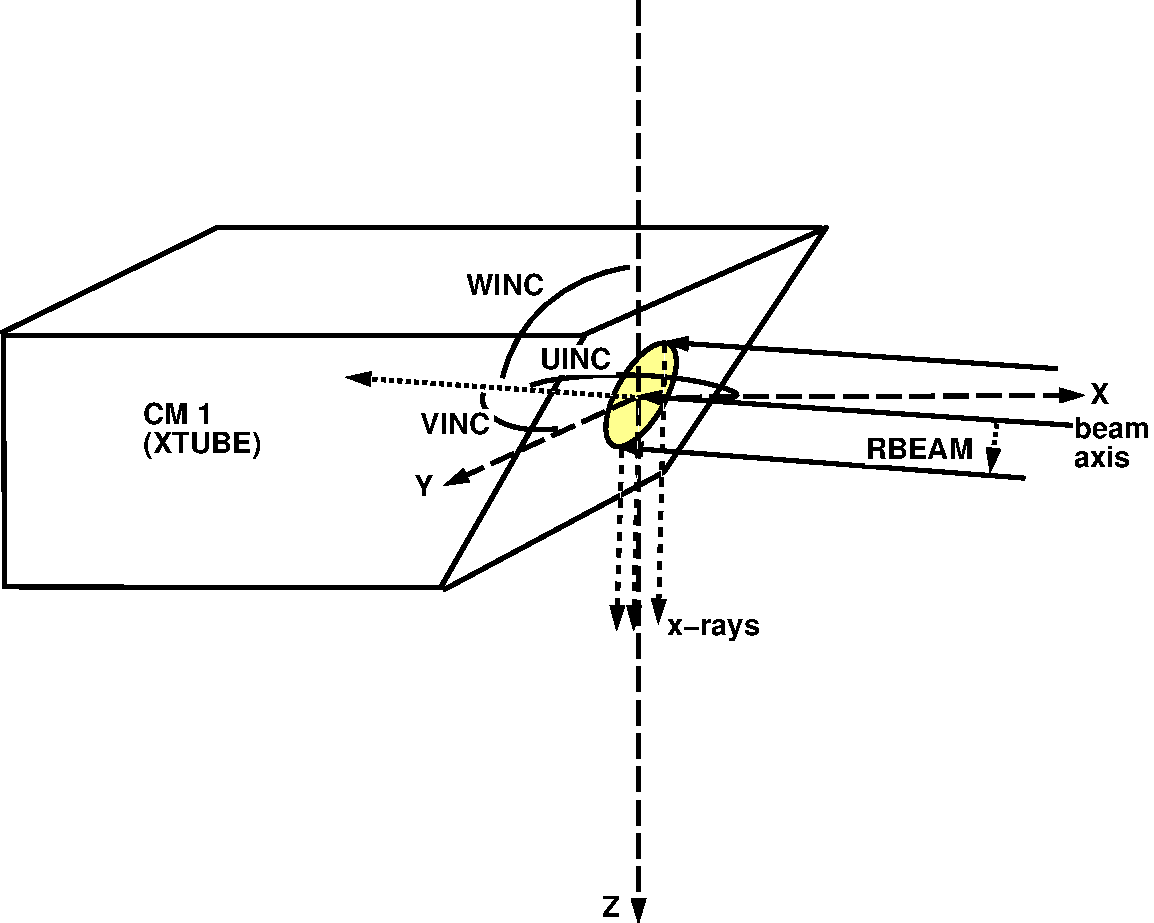
\includegraphics[height=9cm]{figures/src10}
\caption[ISOURC=10: Circular beam for XTUBE.]
{Parallel circular beam incident from the side (ISOURC=10).
This source can only be used with an XTUBE CM as the first CM
position.}
\label{fig_src10}
\end{center}
\end{figure}

\clearpage

\subsection{ISOURC=13: Parallel Rectangular Beam Incident from Side}
\index{source!13 side parallel rectangular beam }
\cen{IQIN, 13, YBEAM, ZBEAM, UINC, VINC}
\index{ZBEAM}
\index{UINC} \index{VINC}
This beam is the rectangular equivalent of ISOURC=10 (see previous
source).
The input parameters for this beam are:
\begin{description}
\item [IQIN] Charge of incident beam (defaults to 0 = photons)
\item [YBEAM] Half-width of beam in cm (defaults to 0.2 cm if set $<$ 0;
defaults to half the thickness of the first CM if set $>$ than this)
\item [ZBEAM] Half-height of beam in cm (defaults to 0.2 cm if set $<$ 0;
defaults to half the thickness of the first CM if set $>$ than this)
\item [UINC] Incident X-axis direction cosine (should be $<$0 so that beam
faces Z-axis; reset to -UINC if it is set $>$ 0)
\item [VINC] Incident Y-axis direction cosine \\
(UINC, VINC default to -1,0 if UINC$^2$+VINC$^2$ = 0)
\end{description}
UINC and VINC are automatically normalized by (UINC$^2$+VINC$^2$).  Note
that the Z direction cosine, WINC, is always assumed to be 0 for this
beam.
\begin{figure}[htbp]
\begin{center}
\leavevmode
\mbox{}\hspace{0cm}
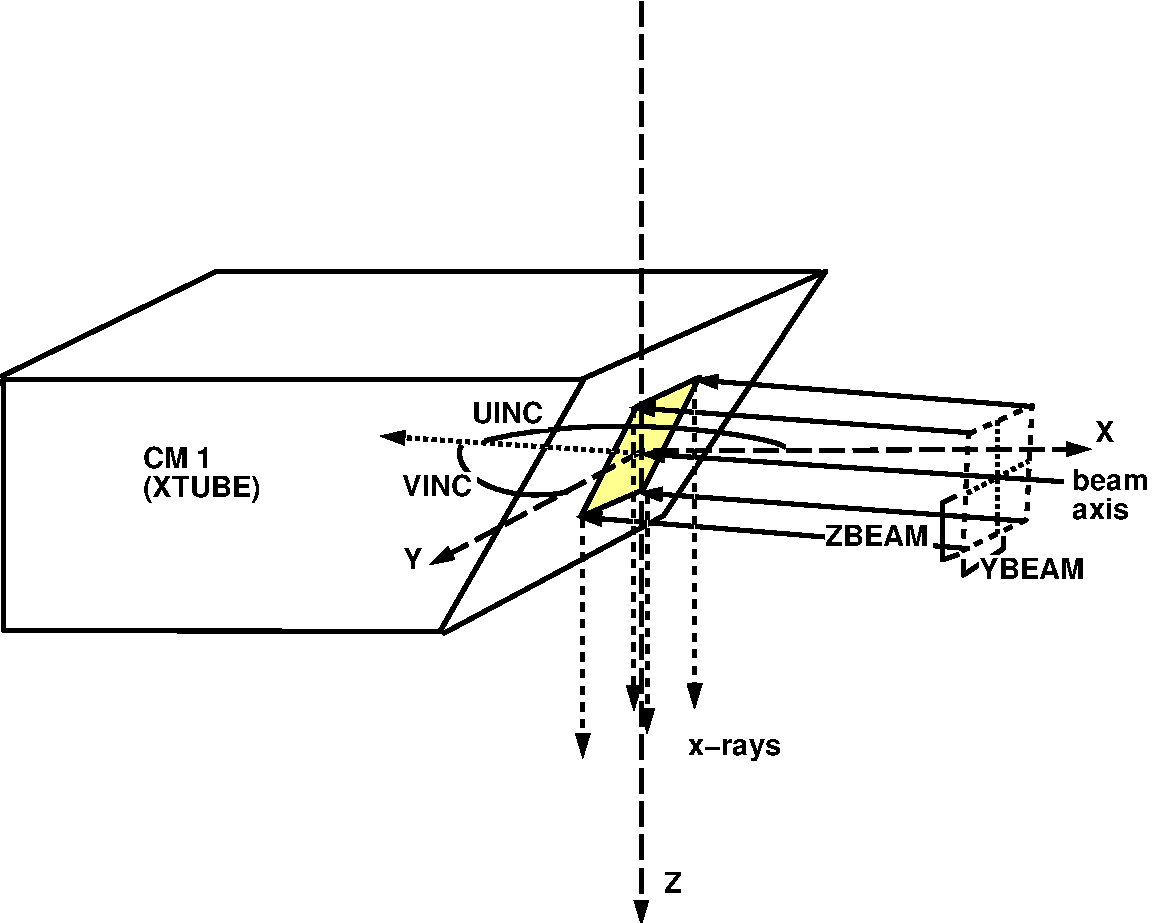
\includegraphics[height=9cm]{figures/src13}
\caption[ISOURC=13: Rectangular beam for XTUBE.]
{Parallel rectangular beam incident from the side (ISOURC=13).}
\label{fig_src13}
\end{center}
\end{figure}

\clearpage
\subsection{ISOURC=15: NRC Swept Beam (Radial Variation,
Divergence)}
\cen{IQIN, 15, GAMMA, ZFOCUS, RTHETAIN, THETAIN \\ SPCNAM}
\index{GAMMA}
\index{RTHETAIN}
\index{THETAIN}
\index{radial intensity distribution}
\index{radial divergence}
\index{swept beam}
\index{ZFOCUS}
\index{source!15 NRC swept beam with radial intensity distribution and
divergence}
This source is similar to the NRC Swept Beam ({\tt ISOURC} = 5) with the
difference that the beam itself has a radially varying intensity
distribution and an angular divergence, both specified by the user.  Also,
the cone swept by the beam has its apex at a user specified Z position,
given by (X=0,Y=0,Z={\tt ZFOCUS}), rather than the apex always being
at (X=0,Y=0,Z={\tt Z\_min\_CM(1)}) as it is in source 5.  As with most
other sources, particles enter from the top of CM 1.

Beam divergence means the beam is diverging or
spreading out about the axis of each element of the swept beam. At any
given instant   each
elemental beam can be thought of diverging from a point on the elemental
beam's axis. This point is specified by the angle ({\tt THETAIN})
created by the elemental beam's axis and a line from the apex to a
point at a specified radius ({\tt RTHETAIN}) in the {\tt ZFOCUS} plane.  This
angle's only role is to define the distance to the apex.

Input parameters for this source are:
\vspace{-3mm}
\begin{description}
\item [IQIN] Charge of the incident beam (defaults to 0 = photons)
\item [GAMMA] Half-angle of the cone swept by the beam in degrees (0$^o$ $\leq$
\verb+GAMMA+ $<$ 90$^o$)
\item [ZFOCUS] Z position of the apex of the swept cone in cm (Note: ZFOCUS can
be greater than, equal or less than {\tt Z\_min\_CM(1)}).
\item [RTHETAIN] The beam radius (in cm)
at which the beam divergence angle, THETAIN, is
defined. {\tt RTHETAIN} must be $>$ 0.
\item [THETAIN] The beam divergence angle (in degrees) at RTHETAIN.  If
{\tt GAMMA} $\neq$ 0, then {\tt THETAIN} can be set to 0; otherwise, it
must be $>$ 0 (Note, however, that it can still be set to such a small
angle that divergence is practically zero).
\item [SPCNAM] The name of file containing beam's radial intensity
distribution about the axis of the elemental beam in a plane at {\tt Z =
ZFOCUS}.
The file \verb+SPCNAM+ has a specific format:
\vspace{-5mm}
\begin{verbatim}
        NRDIST
        (RDISTF(I),RPDF(I),I=1,NRDIST)
\end{verbatim}
\vspace{-5mm}
where:
\index{NRDIST}
\index{RDISTF}
\index{RPDF}
\index{source 15!radial intensity distribution}
\begin{description}
\item [NRDIST] = \# of radial bins in the distribution
\item [RDISTF(I)] = upper radius of bin I in cm
\item [RPDF(I)] = probability (not necessarily normalized) of finding a
                  particle in radial bin I.  These probabilities are multiplied
                  by bin area before sampling.
\end{description}
%\vspace{-3mm}
Some sample radial intensity distribution files are found in {\tt \$OMEGA\_HOME/beamnrc/radial\_source\_distributions}.
\end{description}
The radial position of an incident particle, RIN, is chosen based on
the radial intensity distribution.  The divergence angle, {\tt THETAI}, of the
particle is then
calculated from {\tt TAN(THETAI) = RIN/(RTHETAIN/TAN(THETAIN))}.
Note that the radial distribution is defined at {\tt Z = ZFOCUS} (the apex of the swept
cone) in a plane perpendicular to the Z axis.  This is an approximation since,
strictly speaking, the distribution should be defined in a plane perpendicular
to the beam direction.  However, for {\tt GAMMA} of a
few degrees, this approximation is valid.

In addition to simulating beams more realistically, this source can be
applied to several useful cases. With {\tt GAMMA = 0} and {\tt
THETAIN~$\approx$0}, it can be used to model an arbitrary radial intensity
distribution from a parallel beam incident normally on the front face (
\eg, the distribution could be ring shaped).  With {\tt GAMMA = 0} one
could mimic a point source at a distance from {\tt ZFOCUS} of {\tt
RTHETAIN/tan(THETAIN)} along with a uniform intensity profile out to the
beam radius. One should use source 1 for the uniform case, but could use
source 15 to get an arbitrary radial distribution from a point source.

Figure~\ref{fig_src15} below shows the swept beam source with radial
distribution and divergence.
\begin{figure}[htbp]
\vspace*{-0.35cm}
\begin{center}
\htmlimage{scale=2.0}
\leavevmode
\mbox{}\hspace{0cm}
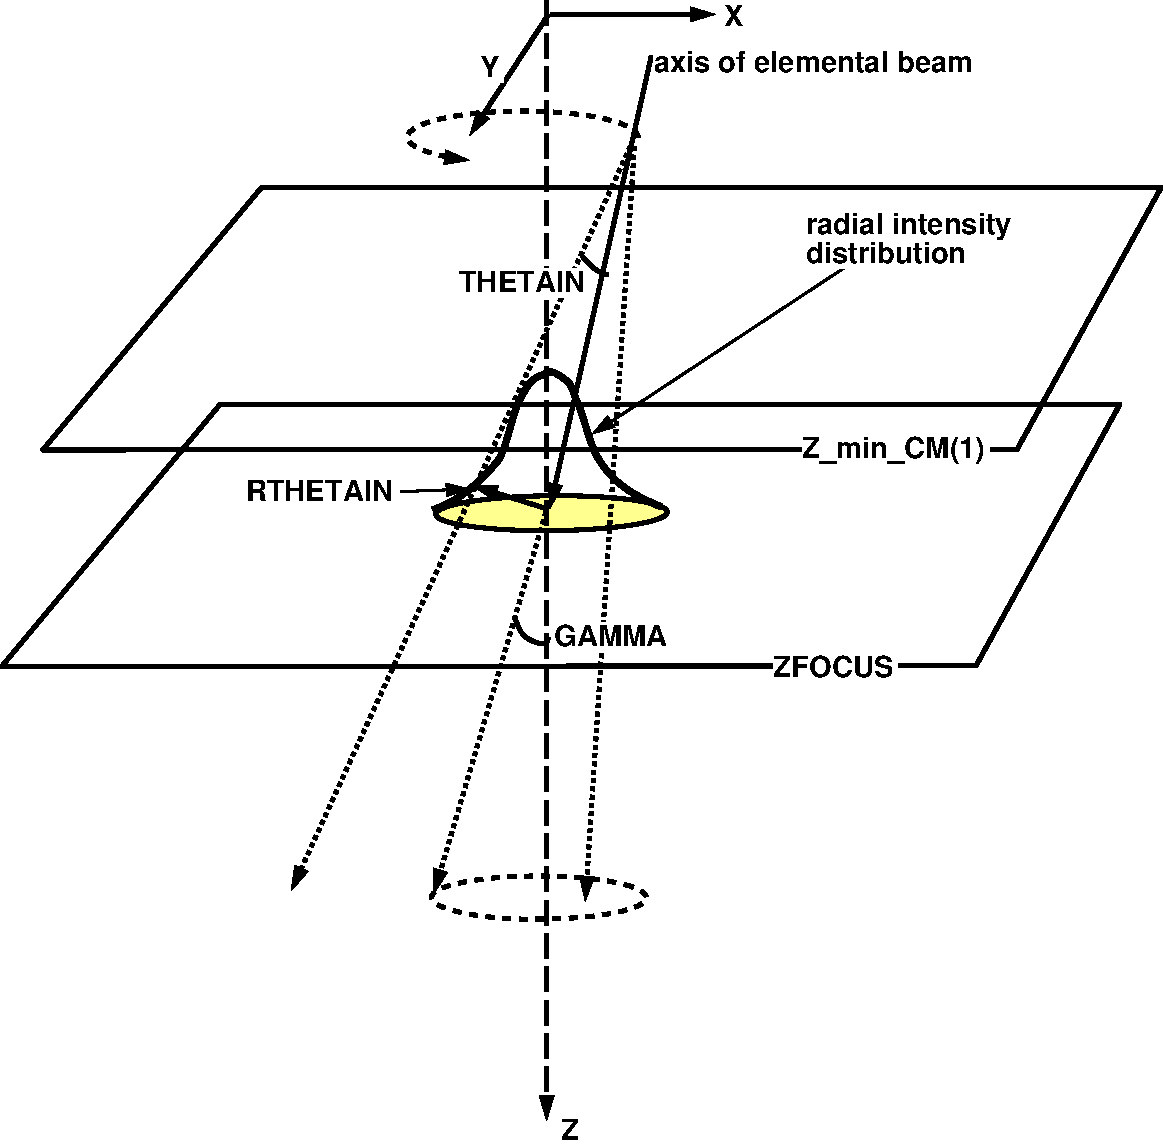
\includegraphics[height=11cm]{figures/src15}
\caption[ISOURC=15: NRC swept beam with radial intensity distribution and
divergence]
{The beam sweeps on the surface of a cone with half-angle {\tt GAMMA} and
with the apex defined at {\tt ZFOCUS}.  The beam itself has a user-defined radial
intensity distribution (in the case shown, a gaussian), defined at {\tt ZFOCUS}
and in a plane perpendicular to the Z axis.  The beam then diverges from this
original distribution as if it originated at an imaginary point back along
the axis of each elemental beam.  The position of this imaginary point is defined by the
divergence angle, {\tt THETAIN}, and the radius (at {\tt ZFOCUS}) at which
the divergence angle is defined, {\tt RTHETAIN}.}
\label{fig_src15}
\end{center}
\end{figure}
\index{GAMMA}
\index{RTHETAIN}
\index{THETAIN}
\index{radial intensity distribution}
\index{radial divergence}
\index{swept beam}
\index{ZFOCUS}

\subsection{ISOURC=19: Elliptical Beam with Gaussian Distributions in X and Y, Parallel or with Angular Spread}
\label{isourc19}
\index{UINC} \index{VINC} \index{WINC}
\index{RBEAM}\index{Z\_min\_CM}
\index{RBEAMY}
\index{source!19 elliptical beam with 2-D Gaussian X-Y distribution}
\vspace*{-0.3cm}
This is an elliptical beam where the ellipse is defined by gaussian intensity distributions
in X and Y.  The beam can either be parallel, with direction cosines
specified by the user, or it can have an angular spread from the Z-axis,
specified by a mean angular spread.
\vspace*{-0.3cm}
\begin{description}
\item [IQIN] The charge of the incident beam (defaults to 0=photons)
\vspace*{-0.2cm}
\item [RBEAM] Standard deviation ($\sigma$) in the X-direction
(if set $>$ 0) in cm, or
-FWHM (FWHM:full-width half-maximum) of the gaussian distribution in the X-direction (if set $<$ 0) in cm.
$\sigma$ is automatically limited to {\tt RMAX\_CM(1)} for circular CM 1 or
$\sqrt{2}${\tt RMAX\_CM(1)} for square CM 1.  If
the user enters {\tt RBEAM}=0, the source collapses to a pencil beam.
\vspace*{-0.2cm}
\item [UINC] X-axis direction cosine (defaults to 0)
\vspace*{-0.2cm}
\item [VINC] Y-axis direction cosine (defaults to 0)
\vspace*{-0.2cm}
\item [WINC] Z-axis direction cosine (defaults to 1, \ie\ parallel to
the z-axis)
\vspace*{-0.2cm}
\item [sigma\_src19] the mean angular spread about the Z-axis.  If
{\tt sigma\_src19}$>$0, then {\tt UINC}, {\tt VINC}, {\tt WINC} automatically
take their default values.
\item [RBEAMY] $\sigma$ (if set $>$ 0) or -FWHM of the gaussian distribution in the
Y-direction in cm.  If set = 0, then {\tt RBEAMY} is set = {\tt RBEAM}, resulting in a circular
beam with a gaussian radial distribution.
\end{description}
\vspace*{-0.3cm}
Note that in the case of a circular beam ({\tt RBEAMY}={\tt RBEAM})
the radial distribution of particles is also gaussian with
$\sigma$ equal to $\sqrt{2}$ times the $\sigma$ of the X and Y gaussian distribution.
\begin{figure}[H]
\vspace*{-0.5cm}
\begin{center}
\htmlimage{scale=2}
\leavevmode
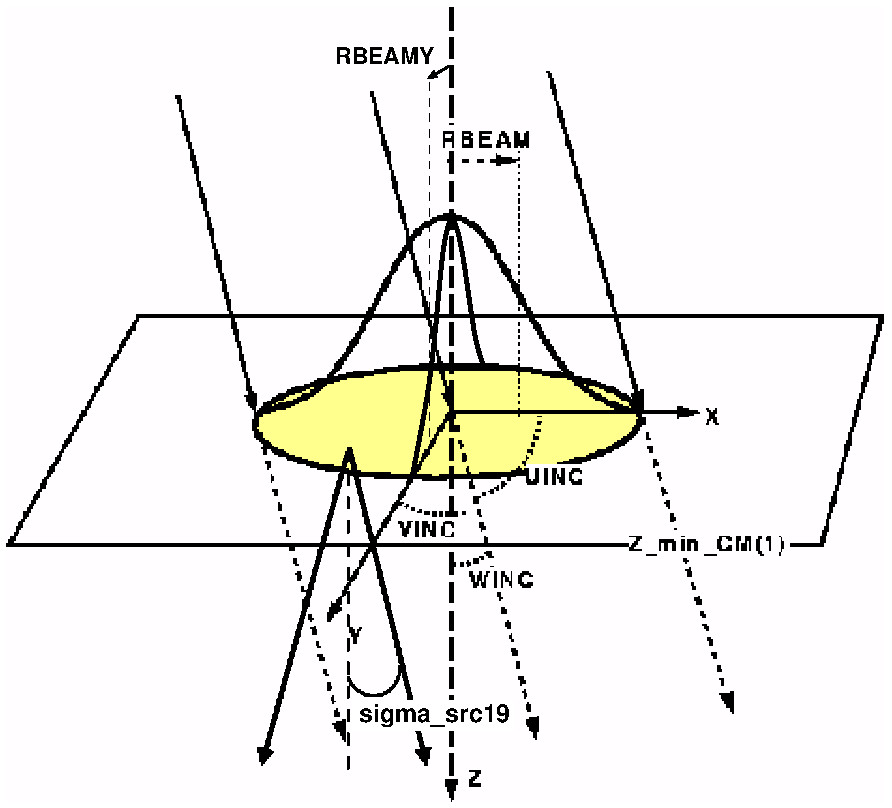
\includegraphics[height=9cm]{figures/src19}
\caption[ISOURC=19: Elliptical beam with gaussian distributions in X and Y.]
{Elliptical Beam with Gaussian Distributions in X and Y (ISOURC=19).  The shape
of the ellipse is defined by {\tt RBEAM} and {\tt RBEAMY} which define the
the $\sigma$ (if set $>$0) or -FWHM of the gaussian intensity
distributions in the X- and Y-directions respectively.
The beam either has a
mean angular spread about the Z-axis, {\tt sigma\_src19}, or, if
{\tt sigma\_src19}$\leq$0, it is a parallel beam with incident direction
cosines specified by {\tt UINC}, {\tt VINC}, {\tt WINC}.}
\label{fig_src19}
\end{center}
\end{figure}

\clearpage

\subsection{ISOURC=21: Phase Space Source}
\label{phspsrcsect}
\index{source!21 phase space}
\index{source!general models}
\index{phase space files!as source}

\cen{IDUMMY, 21, INIT\_ICM, NRCYCL, IPARALLEL, PARNUM, ISRC\_DBS,
RSRC\_DBS, SSDSRC\_DBS, ZSRC\_DBS \\SPCNAM}


This source routine allows a phase space file generated at any scoring
plane to be used as a source in its own right.  Unlike the sources
described thus far, which are assumed to be
incident on the first CM, phase space
sources can be incident on any CM.  They are particularly useful for
doing repeated simulations of lower portions of an accelerator model (\ie\
when the configuration of the lower part of the accelerator is changing,
but repeated simulation of the top part is unnecessary), or simulating
beams made up of several different particle types.
Note that the
\verb+LATCH+ values are passed on when using this source routine and it
is necessary to number \verb+LATCH+ bits consistently between the two
simulations (\ie\ that generating the input file and the current
simulation).  Also, dose and fluence resulting from a phase space source
are normalized by the number of initial particles in the original, non-phase
space source (\ie\ the source that generated the phase space source) and not
by the number of particles incident from the phase space source itself.  More
about this normalization and how it is accomplished appears in section~\ref{PSF} below.
\index{LATCH!in ISOURC=21}
\index{normalization!of dose and fluence when using ISOURC=21}
\index{dose!normalization when using ISOURC=21}
\index{fluence!normalization when using ISOURC=21}

This source can also be used to simulate any incident beam shapes not
covered by the sources described above.  This is done by creating the
appropriate phase space file for the general source by using a stand alone
user-written program and the \verb+phsp_macros.mortran+ macros.
\index{phsp\_macros.mortran}

Input parameters for a phase space source are:
\begin{description}
\item [INIT\_ICM] Component module on which the phase space source is
incident (defaults to 1 if it is set to $<$ 1 or $>$ the number of
\verb+CMs+
in the model)
\index{INIT\_ICM}
\item [NRCYCL] The number of times to recycle each incident particles before
moving on to the next particle in the phase space source.  Thus, each
particle will be used a total of {\tt NRCYCL} + 1 times before moving
on to the next one.  If set $\leq$ 0, then BEAMnrc will automatically
calculate a value of {\tt NRCYCL} based on the number of incident histories
and the number of particles in the phase space file that should prevent
restarting of the phase space source.  If set $>$ 0, the user-input value
is used.  See below for details.
\index{NRCYCL}
\item [IPARALLEL]  No longer necessary if using BEAMnrc's built-in
parallel processing functionality for submitting parallel jobs.  In
previous versions of BEAMnrc, {\tt IPARALLEL} = the number of parallel jobs.
See below for more details.
\index{IPARALLEL}
\item [PARNUM] No longer necessary if using BEAMnrc's built-in
parallel processing functionality for submitting parallel jobs.  In
previous versions of BEAMnrc, {\tt PARNUM}
was set to an integer value in the range 1$\leq${\tt PARNUM}$\leq$
{\tt IPARALLEL}, with a different value of {\tt PARNUM} for each of
the parallel jobs.  See below for more details.
\index{PARNUM}
\item [ISRC\_DBS] Set to 1 if directional bremsstrahlung splitting (DBS)
was used in the BEAMnrc simulation to generate this source {\bf and} you wish to
reject photons directed outside the splitting field (which are fat).  Set to 0
otherwise.
\index{ISRC\_DBS}
\item [RSRC\_DBS] Radius of the DBS splitting field (in cm) used in the
BEAMnrc simulation to generate this source. Only needed if {\tt
ISRC\_DBS} = 1.
\index{RSRC\_DBS}
\item [SSDSRC\_DBS] SSD at which {\tt RSRC\_DBS} was defined in the BEAMnrc
simulation that generated this source (in cm). Only needed if {\tt
ISRC\_DBS} = 1.
\index{SSDSRC\_DBS}
\item [ZSRC\_DBS] Z value where this phase space source was scored
                     in the BEAMnrc simulation (cm).  This will be at the back
                     of a component module (CM).  Note the restriction that
                     {\tt ZSRC\_DBS} is $\leq$ {\tt SSDSRC\_DBS}.
\index{ZSRC\_DBS}
\item [SPCNAM] Filename (with extension) of the phase space source. The full
directory path to the file must be specified.  In the
case of an IAEA-format phase space source, you must supply the full name
of the file containing the phase space data ({\em i.e.} the {\tt .IAEAphsp}
file).  The {\tt .IAEAheader} file will be assumed to be in the same
directory.  For more information on IAEA-format phase space data, see
Section~\ref{iaeasect}.
\end{description}
\index{general source models}

\paragraph{Value of {\tt NRCYCL}}\mbox{}\\
\index{NRCYCL}
{\tt NRCYCL} is an essential input for phase space sources because
phase space data are often sparse, making it necessary to re-use particles
in order to obtain adequate statistics.  However, {\tt NRCYCL} can only
help reduce the inherent uncertainty in the dose calculation. The overall
uncertainty will also be governed by the latent variance of the phase space file (see the
report on history by history
statistics in BEAMnrc and DOSXYZnrc\cite{Wa02a}).
In addition to recycling, particles are also re-used whenever a phase space source is restarted
(which happens automatically when the simulation has used all particles in the
source).  However, restarting may result in an underestimate of
uncertainties~\cite{Wa02a}, making it important to choose a value
of {\tt NRCYCL} that both ensures adequate sampling of the phase space
source and also prevents restarting.

\index{NRCYCL! calculation of}
If you are unsure of the value of {\tt NRCYCL} to use, set
{\tt NRCYCL}$\leq$ 0 and BEAMnrc will automatically calculate its value
based on the number of histories and the total number of particles in the
phase space file.  Even with an automatically-calculated value of
{\tt NRCYCL}, the phase space source may still restart, either because
the algorithm used to calculate {\tt NRCYCL} has determined that
setting {\tt NRCYCL}$>$ 0 will cause the phase space source to
be undersampled, or because some incident particles were
multiple-passers (i.e., had crossed the phase space scoring plane
more than once) and were rejected from the simulation.  If the
phase space source has only been restarted once and only a small fraction
of it has been re-used on the second pass, the effect on uncertainty will not
be significant.  However, if a significant portion of the source has been
re-used on the second pass, or if the source has been restarted more than
once, we recommend re-running the simulation with a new value of
{\tt NRCYCL} given by:
%\begin{footnotesize}
 \[ \hspace*{-1cm}
 \frac{{\tt NCASE}}
 {\left[{\tt NNPHSP-NNPHSP*\left(NPASS\_ph\_sp+NFAT\_ph\_sp\right)}/
 \left({\tt NTOT\_ph\_sp+NPASS\_ph\_sp+NFAT\_ph\_sp}\right)\right]} -1
\]
%\end{footnotesize}
where {\tt NCASE} is the number of histories, {\tt NNPHSP} is the total
number of
particles in the phase space source, {\tt NTOT\_ph\_sp} is the total number
of particles used from the phase space source in
the previous simulation (not including recycling),
{\tt NPASS\_ph\_sp} is the number of particles rejected from the previous
simulation because they
were multiple-passers (not including recycling), and
{\tt NFAT\_ph\_sp} is the number of photons (not including recycling)
rejected because they
fall outside the directional bremsstrahlung splitting field
radius at the SSD (only if {\tt ISRC\_DBS}=1--see below for more
details). {\tt NNPHSP},
{\tt NTOT\_ph\_sp}, {\tt NPASS\_ph\_sp} and
{\tt NFAT\_ph\_sp} can be found in the {\tt .egslst}
file from the previous simulation.
\index{NPASS\_ph\_sp}
\index{NFAT\_ph\_sp}
\index{NNPHSP}
\index{NTOT\_ph\_sp}
\index{NCASE}

Note that, even with {\tt NRCYCL}$>$ 0, the input variable {\tt NCASE}
(see section~\ref{ncasesect}) still controls the number of histories
simulated.  The simulation will stop as soon as {\tt NCASE} histories
have been run, regardless of whether the current particle has been
recycled the full {\tt NRCYCL} times or not.

\paragraph{Inputs {\tt IPARALLEL} and {\tt PARNUM}}\mbox{}\\
\index{IPARALLEL}
\index{PARNUM}
Note: the input variables {\tt IPARALLEL} and {\tt PARNUM} are no longer
necessary if you are using the built-in parallel processing functionality in
BEAMnrc.  In previous versions of BEAMnrc, these inputs were essential
for dividing a phase space source into {\tt IPARALLEL} equal
partitions.  Each job used a different partition given by:
\[ \left({\tt PARNUM}-1\right)*\left(\frac{{\tt NNPHSP}}{{\tt IPARALLEL}}\right)
 <{\tt INPHSP} \leq {\tt PARNUM}*\left(\frac{{\tt NNPHSP}}{{\tt IPARALLEL}}
\right)\]
where {\tt NNPHSP} is the total number of particles in the phase space
source and {\tt INPHSP} is the particle number used.  The Unix
\index{pprocess}
script, {\tt pprocess}, used for parallel job submission with previous
versions of BEAMnrc, set the values of {\tt IPARALLEL} and
{\tt PARNUM} automatically.  You only need to be concerned with these
inputs if you are submitting parallel jobs one by one, manually
creating an input file for each of them.


\paragraph{Inputs re DBS}\mbox{}\\
\index{DBS}
\index{directional bremsstrahlung splitting}
\index{fat photons!rejecting from phase space source}
If directional bremsstrahlung splitting (DBS) was used in the BEAM
simulation used to generate this source, then it is recommended that
you use the inputs {\tt ISRC\_DBS}, {\tt RSRC\_DBS}, {\tt SSDSRC\_DBS}
and {\tt ZSRC\_DBS} to prevent fat photons from compromising dose
or fluence statistics in the current simulation.
{\tt RSRC\_DBS} and {\tt SSDSRC\_DBS}, the radius and SSD of the
DBS splitting field respectively, are available from the DBS inputs for
the BEAMnrc simulation used to generate the phase space source. {\tt ZSRC\_DBS}
will be equal to the Z position of the back of the component module where
this source was scored (this information is available in the {\tt .egslst}
file from the BEAMnrc simulation that generated the source).  When
{\tt ISRC\_DBS} is set to 1, photons in the source are projected along
their trajectory from {\tt ZSRC\_DBS} to {\tt SSDSRC\_DBS}.  If they
fall outside {\tt RSRC\_DBS} at {\tt SSDSRC\_DBS} then they are not
used in the simulation.  In the context of the BEAMnrc simulation that generated
this source, these photons are fat (but this information is not stored
in the phase space file). Note that

Charged particles are never
rejected with this technique, which means that if you do not want fat charged
particles to compromise dose statistics (especially near the surface of a
phantom) then you must use the electron splitting option in DBS.

For more information about DBS, see section~\ref{dbssect} of this manual.

\index{DBS}

\paragraph{3-D and 4-D IAEA phase space sources}
\index{source 21! IAEA format phase space sources}
\index{source 21! with particle Z-position scored}
\index{source 21! with fractional MU index scored}
\index{source 21! 3-D phase space data}
\index{source 21! 4-D phase space data}
Source 21 is capable of handling IAEA format phase space sources in which the (X,Y,Z) position of
each particle is scored (3-D) and/or in which the fractional monitor unit index ({\tt MU}) associated with a
particle is scored (4-D).  This functionality has been adapted from modifications by Lobo \& Popescu\cite{LP10}.

Handling of 3-D phase space data is essential if using accelerator phase space data acquired on a non-planar
surface (such as the data supplied by Varian for their TrueBeam accelerators) or if using phase space
data output by a DOSXYZnrc simulation (see the DOSXYZnrc Users Manual\cite{Wa05}).  If data is scored
in 3-D, this is automatically detected by the source 21 algorithm.  Particles are incident within
a component module (or multiple CMs), and the particle Z-position read from the phase space source
overrides the top of {\tt INIT\_ICM} (see above) as the incident Z-position.  Particles must
be incident within CMs that handle internal sources: SLABS, FLATFILT or SIDETUBE.  If, during a simulation, a
particle is found to be incident within a CM that does not match one of these types, the simulation stops with
an error message.

{\tt MU} is automatically scored in IAEA-format phase space files generated by
accelerator simulations having one or more synchronized CMs with time-varying opening coordinates
(see Section~\ref{CMs} below).  There is also an option to include {\tt MU} in the 3-D phase space files
generated using DOSXYZnrc with a synchronized phase space source or synchronized BEAMnrc simulation
source (see the DOSXYZnrc Users Manual\cite{Wa05}).  {\tt MU} gives a time dimension to the
phase space data.  Hence, this data is termed 4-D.  If {\tt MU} is scored in an IAEA phase space file
being used as a
source, this is automatically detected by the source 21 algorithm.  Instead of choosing a random
value for {\tt MU} at the beginning of each history, a BEAMnrc simulation using a 4-D phase space source uses
the {\tt MU}'s read from the source to set any time-varying opening coordinates of synchronized CMs in the accelerator.
 This allows the CMs to be synchronized with those in the upstream simulation(s) used to generate
the phase space source.

For more information related to phase space sources, see the
section~\ref{PSF} on full phase space files.

\clearpage
\subsection{ISOURC=24: Phase Space Source Incident from User-specified Angle}
\label{Source24}
\index{source!24 phase space from user-specified angle}

\cen{IDUMMY, 24, INIT\_ICM, NRCYCL, IPARALLEL, PARNUM, ISRC\_DBS,
RSRC\_DBS, SSDSRC\_DBS, ZSRC\_DBS \\SPCNAM \\ALPHA24, BETA24, DIST24}

This source is similar to the phase space source (21) with the exception that the
user can specify a point of rotation on the Z-axis above {\tt INIT\_ICM} and rotation
angles about the X- and Y-axes.  Input parameters are the same as {\tt ISOURC}=21 with
additional inputs:
\begin{description}
\item [ALPHA24] Angle of rotation of source (phase-space) plane about an axis
parallel to the X-axis (degrees).
Positive angle is clockwise rotation. -90 degrees $<$ {\tt ALPHA24} $<$ 90 degrees.
\item [BETA24] Angle of rotation of source plane about an axis parallel to the Y-axis (degrees).  Positive angle
is counter-clockwise rotation. -90 degrees $<$ {\tt BETA24} $<$ 90 degrees.
\item [DIST24] Distance of point of rotation above {\tt INIT\_ICM} on the Z-axis (cm).
\end{description}

Note that if either {\tt ALPHA24} or {\tt BETA24} is non-zero {\tt INIT\_ICM} must be $>$ 1,
since any rotation of the source
will result in particles incident from within {\tt INIT\_ICM}-1.  In this case, {\tt INIT\_ICM}
and {\tt INIT\_ICM}-1 must be SLABS, FLATFILT, or SIDETUBE, since these are currently the
only CMs capable of handling particles incident within them.

The initial idea and much of the coding of {\tt ISOURC}=24 is courtesy of Patrick
Downes at University of Cardiff, Wales.

\begin{figure}[H]
\vspace*{-0.4cm}
\begin{center}
\htmlimage{scale=2}
\leavevmode
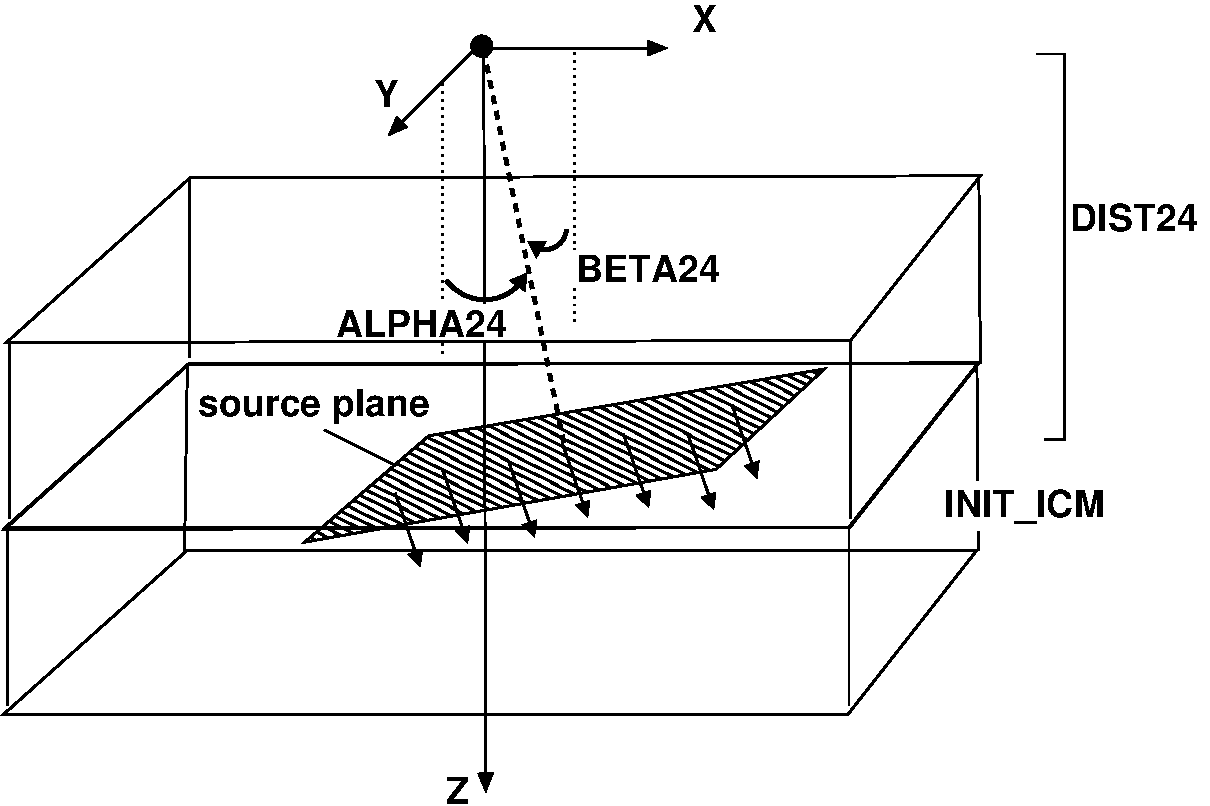
\includegraphics[height=7cm]{figures/src24}
\caption[ISOURC=24: Phase-space Source Incident from User-specified Angle]
{Phase-space source incident from user-specified angle (ISOURC=24).  Similar to
the standard phase-space source (ISOURC=21) except that the user can specify
a point of rotation on the Z-axis above {\tt INIT\_ICM}, {\tt DIST24}, and
angles of rotation about axes parallel to the X-axis, {\tt ALPHA24}, and
Y-axis, {\tt BETA24}.}
\label{fig_src24}
\end{center}
\end{figure}

\clearpage

\subsection{ISOURC=23: BEAM Simulation Source Incident from User-specified Angle}
\label{Source23}
\index{source!23 BEAM simulation source from user-specified angle}

\cen{IDUMMY, 23, INIT\_ICM, ISRC\_DBS, ALPHA24, BETA24, DIST24\\
the\_beam\_code, the\_pegs\_file, the\_input\_file}

This source allows an accelerator that has been compiled as a shared library to
be used as a source in a BEAM simulation.  In function, it is similar to
the phase-space source incident from a user-specified angle, {\tt ISOURC}=24,
but it eliminates the need to store an
intermediate phase space file since the BEAM simulation reads phase-space data at the
scoring plane in
the simulation source directly.  The simulation source runs simultaneously with
and under the control of the BEAM simulation using it, so primary histories in the
simulation source are run each time new phase-space data is required by the
BEAM simulation using it.  Note that this also means that any need to recycle phase
space data is eliminated, another important advantage of the simulation source.

 For information about compiling an accelerator as a shared
library source, the user is urged to refer to Section 4.10.1 in the DOSXYZnrc Users Manual\cite{Wa05}.

Input parameters for source 23 are:
\begin{description}
\index{INIT\_ICM}
\item [INIT\_ICM] CM no. at the top of which the source is incident.
\index{ISRC\_DBS}
\item [ISRC\_DBS] Set to 1 if directional bremsstrahlung splitting (DBS) is used
in the simulation source and you wish to reject fat photons outside the splitting
field.  This is recommended since these photons can compromise statistics in the
downstream BEAM simulation.
\index{ALPHA24}
\item [ALPHA24] Angle of rotation of the source plane about an axis parallel to the X-axis (degrees).
Positive angle is clockwise rotation.
\index{BETA24}
\item [BETA24] Angle of rotation of the source plane about an axis parallel to the Y-axis
(degrees).  Positive angle is counter-clockwise rotation.
\index{DIST24}
\item [DIST24] Distance of point of rotation on the Z-axis above {\tt INIT\_ICM} (cm).
\index{the\_beam\_code}
\item [the\_beam\_code] The name of the accelerator to be used as a simulation source.
This must include the {\tt BEAM\_} prefix ({\em i.e.} {\tt BEAM\_accelname}).  The accelerator
must have been compiled as a shared library on the architecture that the BEAM simulation
is running on.
\index{the\_pegs\_file}
\item [the\_pegs\_file] The name of the PEGS4 data set used by
the simulation source ({\em i.e.} may be different than that used by the BEAM simulation
using the simulation source).
\index{the\_input\_file}
\item [the\_input\_file] The input file for the simulation source.  This must exist in
the directory {\tt BEAM\_accelname}, where {\tt accelname} is the name of the
accelerator being used as the simulation source.  Also, this input file must specify
one phase space scoring plane, and the input parameter {\tt IO\_OPT} must be set
to 1 to output phase-space data at this scoring plane (see Section~\ref{ioopt}.  No phase-space file will be output,
but the phase-space data at this scoring plane will be read directly by the BEAM simulation
using the source.
Note that {\tt the\_input\_file} will specify a value for
{\tt NCASE} (no. of histories) but this will be ignored since the number of histories run
is dictated by the number of incident particles required by the simulation using this
source.
\end{description}

The definitions of the parameters specifying the incident direction, {\tt ALPHA24}, {\tt BETA24} and {\tt DIST24}, are the same as those
for {\tt ISOURC}=24 and shown in Figure~\ref{fig_src24}.  Note that if {\tt ALPHA24} and {\tt BETA24} are
not both 0, then {\tt INIT\_ICM} must be $>$1 since some particles will be incident from within
{\tt INIT\_ICM}-1 and {\tt INIT\_ICM} and {\tt INIT\_ICM}-1 must be of type(s) SLABS, FLATFILT or SIDETUBE.

Unlike the phase-space sources, {\tt ISOURC}=21 and {\tt ISOURC}=24, the only parameter
that needs to be set to reject fat photons from a simulation source using directional bremsstrahlung
splitting (DBS) is {\tt ISRC\_DBS}=1.  This is because information about whether a photon is fat
(directed outside the splitting field) is available directly from the simulation source, so there
is no need to reconstruct the splitting field and the photon's path relative to it.

\index{parallel runs!with a simulation source}
In the case of parallel BEAM runs using a simulation source, each parallel job starts its simulation
source with different random number seeds, ensuring that incident particles are not identical.  This
is in contrast to phase-space sources, where each parallel job uses a different partition, or ``chunk'',
of the phase-space data (see Section~\ref{phspparsect}).
For more information about parallel runs see Section~\ref{parallelcalc}.

\clearpage

\subsection{ISOURC=31: Phase Space Reconstructed Using Beam\\ Models}
\label{Source31}
\index{beam characterization model}
\index{source!31 beam characterization model}

\cen{IDUMMY, 31, CMSOU, SPCNAM}
\index{CMSOU}


This source routine reconstructs the phase space parameters using the beam data
derived from a beam characterization model.  The reconstructed phase space
sources can be incident on any CM.  Use of beam characterization models can
save CPU time for the accelerator head simulation and also result in
significant reduction in disk space requirement for phase-space storage.  For
more information related to beam reconstruction using beam characterization
models, see NRCC report ``Beam Characterization: a Multiple-Source Model'' by
Ma and Rogers (1995).


Input parameters for a beam model source are:

\begin{description}
\item [CMSOU] Component module on which the phase space source is
incident (defaults to 1 if it is set to $<$ 1 or $>$ the number of
\verb+CMs+
in the model)
\item [SPCNAM] Filename (with extension) of the beam model parameters.
\end{description}

By default, this source is not included in the accelerator models. If you
want to include them you must do several things.
\begin{itemize}
\item Copy the files {\tt beammodel\_macros.mortran} and {\tt
beammodel\_routines.mortran} from {\tt \$OMEGA\_HOME/progs/beamdp} to the
directory with you accelerator.

\item Update the {\tt sources.make} file on that same area to include the
above two files.  If you are using a standard accelerator model, you may
just copy {\tt \$OMEGA\_HOME/beamnrc/sources.make.MS} to your accelerator
subdirectory and rename it as {\tt sources.make}.
\index{sources.make}

\item {\tt make} the accelerator
\end{itemize}



\newpage
\section{Monoenergetic vs Energy Spectrum Sources}
\index{source!monoenergetic}  \index{source!energy spectrum}

In any of the above sources, with the exception of the phase space source
(ISOURC=21), incident beam energy can be either monoenergetic or described by an energy
spectrum.  Inputs associated with incident beam energy are:

\begin{description}

\index{MONOEN}
\item [MONOEN] Set to 0 if the beam is monoenergetic (default); set to 1
if the beam energy is described by a spectrum
\index{EIN}
\item [EIN] (required if \verb+MONOEN+ = 0) The kinetic energy of a monoenergetic beam in MeV; defaults
to 1.25 MeV if EIN is set $\leq$ 0
\item [FILNAM] (required if \verb+MONOEN+ = 1) The filename (with extension)
containing information describing the incident beam's energy spectrum
(more on spectrum file format below)
\index{IOUTSP}
\item [IOUTSP] (required if \verb+MONOEN+ = 1) Set to 0 for no summary of the
incident beam energy spectrum in the \verb+.egslst+ output file
(default); set to 1 if a summary is desired
\end{description}

The energy spectrum file, \verb+FILNAM+, has a specific format:
\begin{verbatim}
	SPEC_TITLE
	NENSRC, ENMIN, IMODE
	ENSRCD(I), SRCPDF(I) (I = 1 to NENSRC)
\end{verbatim}
where:
\index{NENSRC}
\index{ENMIN}
\index{IMODE}
\index{ENSRCD}
\index{SRCPDF}
\index{source!energy spectrum}
\begin{description}
\item [SPEC\_TITLE] is an 80-character spectrum title
\item [NENSRC] = \# of energy energy bins in the spectrum histogram
\item [ENMIN] = lower energy of first bin in MeV
\item [IMODE] Set to 0 for histogram counts/bin; set to 1 for counts/MeV
\item [ENSRCD(I)] = upper energy of bin I in MeV
\item [SRCPDF(I)] = probability of finding a particle in bin I (SRCPDF
need not be normalized)
\end{description}
The code randomly distributes incident particle energies equally across
each energy bin.

On \verb+$HEN_HOUSE/ensrc_spectra+ there are a collection of spectra
developed at NRC over the years in various situations.  We intend to
augment this collection with time, and will happily add any other
spectra sent to us in the correct format, and with some semi-adequate
documentation.
\index{ensrc\_spectra}
\index{energy spectra!for sources}
\index{spectra!for sources}

\newpage
\section{Variance Reduction in BEAMnrc}
\index{variance reduction}
There is an extensive discussion of variance reduction in BEAM in the
original BEAM paper \cite{Ro95}.

\subsection{Range Rejection}
\label{RR}
\index{variance reduction!range rejection}
\index{range rejection}
\index{ECUT}
\index{ECUTRR}

This section contains a brief description of how range rejection
is performed and describes the input variables used to control range
rejection.

Range rejection is used to save computing time during simulations.  The
basic method is to calculate the range of a charged particle and
terminate its history (depositing all of its energy at that point)
if it cannot leave the current region with
energy $>$ {\tt ECUTRR}.  {\tt ECUTRR} is the range
rejection cutoff energy which may vary
from region to region depending on the type of range rejection used
(see below).
\index{ECUTRR}
\index{ECUTRR!definition}  To
determine the range to {\tt ECUTRR}, BEAMnrc calculates the range from
{\tt ECUTRR} to {\tt AE} (using EGSnrc macros and EGSnrc-calculated
tables of range to {\tt AE} as a function of electron energy) for each
region at the beginning of the simulation (zero if {\tt ECUTRR} = {\tt AE}).
Then, before each charged particle
step during the simulation, this value is subtracted from the particle's
{\tt range} to {\tt AE} (which is always calculated by EGSnrc).
Ranges are calculated using restricted stopping powers and, thus,
represent
the longest possible ranges to {\tt ECUTRR}.

When the range rejection control variable
\verb+IREJCT_GLOBAL+ is set to 2, range rejection is
performed on a region-by-region basis.  In this case {\tt ECUTRR} in
each region is simply equal to the value of {\tt ECUT} in the region.
If the range to {\tt ECUTRR} is less than the perpendicular distance to
the nearest region boundary,
the history is terminated and energy is deposited in the current region.
On the other hand,
\index{IREJCT\_GLOBAL}
when \verb+IREJCT_GLOBAL+ is set to 1, {\tt ECUTRR} is the minimum energy
that a charged charged particle can have as it
leaves the current region and still reach the bottom of the
\index{ECUTRR}
accelerator with an energy greater than the global \verb+ECUT+.
\verb+ECUTRR+ is automatically calculated for each region at the beginning of
the simulation.  Similar to {\tt IREJCT\_GLOBAL=2}, if the range to
\verb+ECUTRR+ is less than the perpendicular distance to the nearest region
boundary, the
particle is terminated and energy deposited in the current region.
\verb+IREJCT_GLOBAL=1+ can save more time than
\verb+IREJCT_GLOBAL=2+ but can only be used if
there is only 1 scoring plane and it is at the very bottom of the
accelerator.  One can approximate \verb+IREJCT_GLOBAL=1+ for other
situations by using \verb+IREJCT_GLOBAL=2+ and carefully selecting
\verb+ECUT+ for different regions throughout the accelerator.

\index{range rejection}
Range rejection introduces an approximation because, in
terminating a charged particle's history and depositing all of its
energy in the current region, it is assumed that any bremsstrahlung photons that
would have been created by the particle, do not leave the current
region.  The user can minimise inaccuracies resulting from this approximation
using the input variable
\verb+ESAVE_GLOBAL+ defining the maximum charged
particle energy (in
\index{ESAVE!ESAVE\_GLOBAL}
MeV) at which
range rejection is considered.  The choice of
\verb+ESAVE_GLOBAL+ depends on
the incident beam energy and the materials that it is passing through.
\verb+ESAVE+ is treated internally on a region by region basis, but only
in the CM SLABS does the user currently have the ability to assign
individual values to each region (via \verb+ESAVEIN+,
this is because this CM is used for
bremsstrahlung targets and we thought we might need more control).

The actual rejection of particles based on range to {\tt ECUTRR}
is performed in a BEAMnrc macro and does
not make use of the internal range rejection macro available in EGSnrc.
This is because the EGSnrc macro only performs range rejection based on
range to {\tt AE}.
\index{ESAVE}
\index{ESAVE!ESAVEIN}

\subsection{Photon Forcing}
\index{variance reduction!photon forcing}
\index{photon forcing}
\index{forcing}

BEAMnrc offers an option whereby the user can force photons to interact
in specified CMs within  a simulation.  This option is useful for improving
statistics of scattered photons when photon
interactions are sparse (\eg\ in thin
slabs of material or in material with low density).  One of the main
purposes of implementing this option was to study the generation of
contaminant electrons in a photon beam.
\index{contaminant electrons}

Briefly, a photon forced to interact in a CM is ``split'' into a
scattered photon whose weight is equal to the probability of interaction
and an unscattered photon carrying the remaining weight.  The unscattered
photon proceeds as if an interaction did not take place, and it cannot be
forced to interact any more within the specified forcing zone, which can
consist of one or several component modules.  However, once the
unscattered photon gets out of the forcing zone, it may interact again
depending on the sampled pathlength. The scattered photon can be forced
again in the forcing zone depending on how many interactions are allowed
to be forced.

The input variables used to control photon forcing are:
\index{IFORCE}
\index{NFMIN}
\index{NFMAX}
\index{NFCMIN}
\index{NFCMAX}
\begin{description}
\item [IFORCE] Set to 0 for no forcing (the default); set to 1 for photon
forcing
\item [NFMIN] Photon interaction \# at which to begin forcing (defaults to 1).
Currently, the option to start photon forcing at any interaction other than the
first one in the forcing CMs has been disabled.  Thus, {\tt NFMIN} is
effectively 1 regardless of what is input.
\item [NFMAX] Photon interaction \# after which to stop forcing (defaults to 1)
\item [NFCMIN] CM \# at which to start forcing (defaults to 1)
\item [NFCMAX] CM \# beyond which to stop forcing (defaults
to the \# of  \verb+CMs+ in the accelerator)

\end{description}
\index{forcing} \index{photon forcing}

Photon forcing parameters are passed onto secondary photons, so that
if the parent particle has not yet been forced to interact {\tt NFMAX}
times, each secondary photon is forced to interact the remaining number
of times (\ie\ {\tt NFMAX} - \# of times parent particle forced) as long
as it is within the forcing CMs.  Forcing of secondary photons does not
affect the number of times the parent particle is forced to interact
if it is a photon as well.  The feature of passing forcing parameters
to secondary photons is particularly useful to get good statistics for
bremsstrahlung photon interactions.  The incident electron creating the
photons will not be forced at all, so each bremsstrahlung photon will be
forced to interact {\tt NFMAX} times.  This feature makes Photon Forcing
a powerful tool for improving statistics when used in conjunction with
bremsstrahlung splitting (see next section).

Note that forcing in restricted regions with low mass can lead to a few
electrons created outside the forcing region having much larger weights than
those created inside the forcing region and thereby distorting results
which are sensitive to these weight variations.

\subsection[Brem Splitting and Russian Roulette]
               {Bremsstrahlung Photon Splitting and Russian Roulette}
\label{bremsection}
\index{variance reduction!bremsstrahlung splitting}
\index{bremsstrahlung!Russian Roulette with splitting}
\index{bremsstrahlung!splitting}
\index{Russian Roulette}

Bremsstrahlung photon splitting offers the user another variance
reduction technique which improves the statistics of
bremsstrahlung photons resulting from electron interactions.
The technique has been described for general use in EGS in
references~ \cite{Bi89,RB90}.  BEAMnrc offers two bremsstrahlung splitting
techniques, uniform bremsstrahlung splitting (UBS) and
directional bremsstrahlung splitting (DBS).  Prior to 2013, BEAMnrc
also supported selective bremsstrahlung splitting (SBS).  However,
this has been superseded by the more efficient DBS.  UBS
has been
optimised in BEAMnrc with the addition of the Russian Roulette feature
(not required for DBS).

\subsubsection{Uniform Bremsstrahlung Splitting}
\index{UBS}
\index{uniform bremsstrahlung splitting}

Input variables associated with uniform bremsstrahlung splitting (UBS) are:
\index{IBRSPL}
\index{NBRSPL}
\begin{description}
\item [{\tt IBRSPL}] Set to 1 for uniform bremsstrahlung splitting
\item [{\tt NBRSPL}] The splitting number.  Also applied to higher-order\\
bremsstrahlung and annihilation photons if Russian Roulette
is on (see section~\ref{rusrousect} below).
\end{description}

Each bremsstrahlung event produces {\tt NBRSPL} photons, each having a weight
equal to $\frac{1}{{\tt NBRSPL}}$ times the weight of the electron that
underwent the bremsstrahlung event.  The energies and directions of each
photon are sampled individually according to the relevant probability
distributions.  The energy of the primary electron is decremented by
the energy of just one of the photons.  This must be done in order to
preserve the effects on energy straggling but it does mean that energy is
not conserved on a given history (the energy would have to be decremented
by the average energy of the photons created) but it is conserved ``on
average'' over many histories.

The splitting number, {\tt NBRSPL}, is not applied to higher-order
higher-order bremsstrahlung and annihilation photons unless
Russian Roulette is turned on (see section~\ref{rusrousect}
below).  This prevents wasting simulation time by tracking many
higher-order photons of vanishing weight.

Uniform bremsstrahlung splitting in BEAMnrc is now handled by the EGSnrc
system using a more efficient internal bremsstrahlung splitting feature.
So, other than input, there is no longer any coding in BEAMnrc related
to this except for the feature which turns it off for higher orders.

\subsubsection{Selective Bremsstrahlung Splitting}
\label{sbssect}
\index{SBS}
\index{selective bremsstrahlung splitting}

Selective bremsstrahlung splitting (SBS) has been superseded by
directional bremsstrahlung splitting (DBS) (see section~\ref{dbssect} below) and is no longer
supported.

\subsubsection{Charged Particle Russian Roulette}
\label{rusrousect}
\index{Russian Roulette}

Note that directional bremsstrahlung splitting (DBS), described in
section~\ref{dbssect} below does not make use of this
charged particle Russian Roulette input.

When using UBS, following all of the secondary charged particles
created by the
``split'' photons increases
the CPU time required for simulations.
If the primary interest is in
secondary electrons or their effects (\eg\ dose deposition), the extra
computing time is obviously acceptable.  But if, as is often the case, the
main interest is in the bremsstrahlung photons themselves, one can reduce
the CPU time while still preserving the variance reduction advantages of
bremsstrahlung splitting by using a Russian Roulette technique with any
charged particles generated by the split photons.

The possible settings of the Russian Roulette input, {\tt IRRLTT}, are:
\index{IRRLTT}

\begin{description}
\item[= 0] Russian Roulette off.  No splitting of higher-order
           bremsstrahlung annihilation photons.
\item[= 1] Option discontinued.  This defaults to {\tt IRRLTT}=2 (see below).
\item[= 2] Russian Roulette on.  Higher-order
           bremsstrahlung and annihilation photons are split
           with splitting number {\tt NBRSPL} in UBS.
\end{description}

Russian Roulette is implemented by giving secondary charged particles
resulting from split photons a survival threshold.  The survival threshold
is always the inverse of the photon splitting number.  Thus, in the case of
UBS, the threshold is fixed and is equal to $\frac{1}{NBRSPL}$.
Then a random number is chosen for each charged
particle.
If the random number is less than the survival threshold,
the charged particle survives, and its weight is increased by
a factor of {\tt NBRSPL}.
Otherwise, the charged particle is eliminated.
Secondary charged particles subject to Russian Roulette are electrons
resulting from Compton events and photoelectric events and electrons
and positrons resulting from pair production.

Note that if Russian Roulette is turned on, then higher-order
bremsstrahlung and annihilation photons are also
split.  This is because any charged particle
surviving Russian
Roulette has a weight higher than the photon that created it.  If
radiative products from this surviving charged particle are not split, then
their high weight may interfere with the statistics of the original
split bremsstrahlung photons.  Also, splitting of
higher-order bremsstrahlung and annihilation photons does not greatly increase
computing time when Russian Roulette is on because most of the secondary
charged particles have been eliminated.

For a more complete description of Uniform Bremsstrahlung Splitting and Russian
Roulette, see the BEAM paper \cite{Ro95}.


\subsubsection{Directional Bremsstrahlung Splitting (DBS)}
\index{directional bremsstrahlung splitting}
\index{DBS}
\label{dbssect}
\paragraph{DBS inputs}\mbox{}\\
Directional bremsstrahlung splitting was introduced into
BEAMnrc in 2004 and results in greater efficiency than SBS\cite{Ka04a}.
Our results have shown that using DBS in a photon beam can
result in fluence efficiencies up to 8 times higher than with
SBS (up to 20 times higher than with UBS) and dose efficiencies up
6 times higher than with SBS (up to 26 times higher than with UBS).  The
actual improvements will depend upon the energy and other details of
the photon beam being simulated.

DBS began from the same philosophy as SBS, in which bremsstrahlung photons
aimed into a field of interest (encompassing the treatment field) are
split at the time of creation, while those aimed away from the field are
not.  Beyond that, however, the two algorithms are completely different.

The input parameters for DBS are:

\index{IBRSPL}
\index{NBRSPL}
\begin{description}
\item [{\tt IBRSPL}] Set to 2 for directional bremsstrahlung splitting
\item [{\tt NBRSPL}] Splitting number.
Set to $\approx$1000 if you are using charged particle splitting
(see below) or $\approx$5000 if not.  Note that {\tt \$MXSTACK} in
the file {\tt beamnrc\_user\_macros} must be increased to avoid
overflows and to be safe, should probably be an order of magnitude larger
than {\tt NBRSPL}.
\index{\$MXSTACK}
\item [{\tt FS}]  The radius of the DBS splitting field in cm.  This
must at least encompass the entire treatment field and should go sufficiently
beyond the edges of the treatment field that the contribution of fat
photons from outside the splitting field (see below for
more details) to dose below {\tt SSD} is negligible.
For a 10$\times$10 cm$2$ field,
we recommend {\tt FS}=10 cm.
\index{DBS!FS}
\index{FS}
\item [{\tt SSD}]  The Z value (in cm)
at which the above {\tt FS} is defined.
\index{DBS!SSD}
\index{SSD}
\item [{\tt ICM\_DBS}] The component module (CM) number in which
electron (charged particle) splitting is to take place.  Set this equal to
the CM number modeling the flattening filter in your accelerator.
Note that electron splitting is enabled in FLATFILT and PYRAMID CMs, so
one of these, likely FLATFILT, must be used to model the flattening filter.
If {\tt ICM\_DBS} is set to 0, then electron splitting is turned off.
\index{ICM\_DBS}
\item [{\tt ZPLANE\_DBS}] The plane number in CM no. {\tt ICM\_DBS} at which
electron splitting will take place.  Planes correspond to layer boundaries
within the CM.  Set this equal to the
back surface of the flattening filter (i.e., {\tt ZPLANE\_DBS}=no. of
layers in flattening filter + 1).
\index{ZPLANE\_DBS}
\item [{\tt IRAD\_DBS}] Set to 1 to redistribute the {\tt NBRSPL} split
charged particles in a radially-symmetric manner about the Z axis.  This
can improve charged particle statistics if your beam is radially
symmetric.
\index{IRAD\_DBS}
\item [{\tt ZRR\_DBS}] The Z position of the Russian Roulette plane
used in conjunction with charged particle splitting (see below for
more details).  Place this several mm above the splitting plane, still
within the flattening filter.
\index{ZRR\_DBS}

\item[{\tt Use a rejection plane} {\tt [USE\_REJPLN]}] Options are {\tt ON} or
{\tt OFF}. If {\tt Use a rejection plane= On} then define
a {\em rejection plane} which discards fat photons and
fat charged particles if they interact below the rejection plane. This
prevents correlated split photons from being created close to the
scoring plane and degrading the statistics of the scored
quantities. Our Monte Carlo studies show that eliminating these fat
particles has a negligible effect on fluence scoring\cite{AR07} and
dose scoring\cite{Ka04a} for typical field-sizes of interest. The
rejection plane is meant to be placed in the air layer between the
bottom of the last component in the accelerator geometry and the
scoring plane.  This input
must appear between the delimiters
{\tt :Start DBS rejection plane:} and
{\tt :Stop DBS rejection plane:} at the end of the input file.
See below for more details.

\index{rejection plane}
\index{USE\_REJPLN}

\item[{\tt Z(cm) from zero reference plane} {\tt [Z\_REJPLN]}]
The distance, in cm, between the rejection
plane and the plane where Z=0. If the scoring plane
is at an SSD = 100 cm, then a typical {\tt Z\_REJPLN} could be between
50 and 90 cm.
This input must appear between the delimiters
{\tt :Start DBS rejection plane:} and
{\tt :Stop DBS rejection plane:} at the end of the input file.
See below for more details.
\index{Z\_REJPLN}

\end{description}

\index{Z\_REJPLN!input format}
\index{USE\_REJPLN!input format}
Both the {\tt USE\_REJPLN} and {\tt Z\_REJPLN} differ from other
DBS-related inputs in that they must appear between
delimiters {\tt :Start DBS rejection plane:} and
{\tt :Stop DBS rejection plane:} in the
{\tt .egsinp} file.  For example, the following input
defines a rejection plane at Z=22.5 cm:
\begin{verbatim}
:Start DBS rejection plane:

 Use a rejection plane= On
 Z(cm) from zero reference plane= 22.2

:Stop DBS rejection plane:
\end{verbatim}
This section must appear in the {\tt .egsinp} file somewhere below the input
for the last component module.  Note that the
BEAM GUI automatically reads/writes the rejection plane
inputs in the correct format, so in practice the user does
not need to concern themselves with it.

\paragraph{Outline of the DBS algorithm}\mbox{}\\
If a charged particle undergoes a bremsstrahlung or
annihilation event, then
DBS splits this event {\tt NBRSPL} times.  The resultant photons
all have their weight multiplied by {\tt NBRSPL}$^{-1}$.  DBS
then loops through these split photons and for each one,
determines whether or not it is aimed into the splitting field
defined by {\tt FS} and {\tt SSD}.  If it
\index{fat photons} \index{non-fat photons}
is, then the photon is kept and is considered ``non-fat'' (low-weight).
If not, then Russian Roulette is played
on the photon by comparing a random number to a survival threshold of
{\tt NBRSPL}$^{-1}$.  If the random number is less than this number,
then the photon is kept and its weight is multiplied by
{\tt NBRSPL} and it is considered a ``fat'' (high-weight) photon.  Splitting
is not limited to bremsstrahlung and annihilation events, however.
If one of these
fat photons undergoes a Compton event, then it is also split {\tt NBRSPL}
times and the same Russian Roulette scheme as above is applied to
photons not aimed into the splitting field.  Moreover, the basic DBS
algorithm eliminates all but a few charged particles by:
\begin{enumerate}
\item playing Russian Roulette (survival probability {\tt NBRSPL}$^{-1}$)
with all electrons resulting from a split Compton event
\item requiring ``non-fat'' photons (ie low-weight photons that are
actually aimed
into the splitting field) to survive Russian Roulette
(survival probability {\tt NBRSPL}$^{-1}$) before they can undergo
pair production, photoelectric or Compton events.  This condition
is relaxed if the event is about to happen in a gas ($\rho<1.2\times10^{-2}$
g/cm$^3$) to prevent fat photons (ie survivors of Russian Roulette)
from being generated in the air just above the splitting field and then
Compton scattering into the field, thus compromising the photon statistics.

\end{enumerate}
It can be seen that, other than non-fat charged particles generated in the air
just above the splitting field due to the exception in (2) above,
those few charged particles that do survive will have a high weight
(ie will be fat).

DBS results in many non-fat photons inside the
splitting field and few fat photons outside the splitting field.  All of the
non-fat photons inside the splitting field will have the same low weight
({\tt NBRSPL}$^{-1}$ times the weight of the incident particles).  This
is desirable since a large
variation of weights inside the field was one factor compromising
the efficiency of SBS.

DBS as described thus far is very efficient for photon fluence/dose, however
it will result in only a few fat charged particles reaching the SSD.
If you are interested in the charged particle contribution to dose
(as in most realistic cases), you must use
the electron (really, charged particle) splitting function to
``recover'' the charged particles.

The inputs for electron splitting are {\tt ICM\_DBS}, {\tt ZPLANE\_DBS},
{\tt IRAD\_DBS} and {\tt ZRR\_DBS}.  {\tt ICM\_DBS} and {\tt ZPLANE\_DBS}
define a CM number and a plane number (which will correspond to a layer
boundary) within that CM at which all fat charged particles are to be
split {\tt NBRSPL} times (with their weights multiplied by
{\tt NBRSPL}$^{-1}$).  If you have set {\tt IRAD\_DBS}=1, then these
split charged particles will be redistributed in a radially-symmetric
manner about the beam axis.  Radial redistribution can result in
better statistics as long as the beam has radial symmetry above the
electron splitting plane.  {\tt ZRR\_DBS}
defines a ``Russian Roulette plane'' which is always above the
electron splitting plane. Below this Russian Roulette plane, DBS is carried out
in the following manner:
\vspace*{-4mm}
\begin{enumerate}
\item electrons resulting from a split Compton event are not
subject to Russian Roulette
\item non-fat photons undergo pair production, photoelectric
and Compton events
\item If a fat photon (i.e., one not aimed into the splitting field) undergoes a
pair production or photoelectric event, then the event is split
{\tt NBRSPL} times to create {\tt NBRSPL} (photoelectric) or 2*{\tt NBRSPL} (pair
production) non-fat charged particles.
\end{enumerate}
\vspace*{-4mm}
Together, use of the splitting and Russian Roulette planes ensures that
all charged particles reaching the SSD are non-fat (and that there are many of
them).

\paragraph{DBS parameter selection}\mbox{}\\
We have found that, although optimal settings of the DBS splitting parameters
depend on the details of the accelerator being simulated, some generalizations
can be made.  {\tt NBRSPL}, the splitting number, should be set
$\approx$1000 for peak efficiency if you are also using electron splitting.
If electron splitting is off, then peak efficiency occurs at
higher splitting numbers ($\approx$5000).  The splitting field radius
{\tt FS}, must at least enclose the entire beam field.  However, it should
also go sufficiently beyond the edges of the beam field that the
dose contribution below the SSD from fat photons
(from outside the splitting field) is negligible
(more about this below).  The efficiency
of DBS decreases with increasing {\tt FS}, so it is desirable to
select the smallest {\tt FS} possible that still provides adequate coverage.
We have found that for a 10$\times$10 cm$^2$ field,
a splitting field radius of 10 cm goes sufficiently beyond the edges without
a significant sacrifice in efficiency.  If you
are in doubt about how far beyond the edges of the beam field the splitting
field should go, it is okay to overestimate by up to 5 cm,
and the gain in efficiency
will still be significantly greater than UBS or SBS.

If you are using electron (charged particle) splitting, then you must
select the locations of the splitting and Russian Roulette planes.
We have found that the optimum location for the splitting plane is at
the very back (ie downstream surface) of the flattening filter, with
the Russian Roulette plane slightly above this.  Because of the
way electron splitting is coded, the splitting plane is specified
by a CM number, {\tt ICM\_DBS}, and then a plane number,
{\tt ZPLANE\_DBS}, within that CM.  Thus, {\tt ICM\_DBS}
should correspond to the CM modeling the beam flattening filter.
Currently, splitting is
only enabled in the FLATFILT and PYRAMID CMs, so this means that your flattening filter
must be modeled with one of these, likely FLATFILT.  If you are using the BEAM GUI, input of
{\tt ICM\_DBS} is made easier by only presenting the user with a list of
the FLATFILT and PYRAMID CMs in the accelerator.
Planes within a CM correspond to layer
boundaries in the geometry, so to place the splitting plane at the
very back of the flattening filter, set {\tt ZPLANE\_DBS}=(no. of layers
in flattening filter + 1).  Again, GUI input makes selection of
{\tt ZPLANE\_DBS} easier by showing the user a list of possible
planes (along with their Z positions) within CM number {\tt ICM\_DBS}.

Finally, the user must select {\tt ZRR\_DBS}, the Z position (in cm) of the
Russian Roulette plane.  {\tt ZRR\_DBS} should be several millimeters
above the splitting plane, but its exact value is not critical, since,
with the eception of a sharp drop in efficiency when the
{\tt ZRR\_DBS} is $<$ 1 mm above the splitting plane,
the overall variation in efficiency with distance between the Russian
Roulette and splitting planes is small.
In a simulated 6 MV beam (10$\times$10 cm$^2$ field) from an SL25
accelerator, Russian Roulette was optimized with
the splitting plane at Z=15.66 cm (the back of the flattening filter),
and the {\tt ZRR\_DBS}=15.5 cm.
\index{ICM\_DBS}
\index{PLANE\_DBS}
\index{ZRR\_DBS}

\paragraph{Augmented range rejection with DBS}\mbox{}\\
\index{range rejection!augmented with DBS}
When using DBS with electron splitting
and charged particle range rejection in the simulation,
the user has the option to use an augmented range rejection scheme which
is more efficient.  If you are using the BEAMnrc GUI, this is selected
by clicking on the ``Augmented range rejection'' checkbox in the DBS
input frame.  If you are editing the {\tt .egsinp} file directly, then
this option is selected by changing the {\tt IREJCT\_GLOBAL} input
(see Section~\ref{RR}) to -{\tt IREJCT\_GLOBAL} ({\em e.g.} if you
had originally set {\tt IREJCT\_GLOBAL}=2, for region-by-region range
rejection, then set {\tt IREJCT\_GLOBAL}=-2 for augmented
region-by-region range rejection with DBS).
Augmented range rejection is identical to the
standard range rejection selected
(see Section~\ref{RR}) with the
exception that all non-fat charged particles
(which will exist only if electron splitting is
being used with DBS) that cannot make it
to the nearest region boundary with energy $>$ {\tt ECUT} are subject
to Russian Roulette (survival probability=1/{\tt NBRSPL}) regardless
of whether or not their energy is greater than the range rejection
cutoff energy ({\tt ESAVE\_GLOBAL}).  Recall that in the standard
schemes, range rejection
is not considered if the particle energy is $>$ {\tt ESAVE\_GLOBAL}.  The
augmented scheme does not influence bremsstrahlung production, since particles
that survive the Russian Roulette (with their weight increased by a factor of
{\tt NBRSPL}) still have a chance to undergo bremsstrahlung events.
Preliminary studies in a simulated 6 MV photon beam
have shown that augmented range rejection can reduce the CPU time
by $\sim$20\%.  Note that if you have
edited the {\tt .egsinp} file and set {\tt IREJCT\_GLOBAL}$<$0
but are not using DBS, then standard range rejection corresponding to
{\tt IREJCT\_GLOBAL}=$|${\tt IREJCT\_GLOBAL}$|$ is done.


\index{total-fat dose}
When DBS is used in BEAM, an additional dose component (see
Section~\ref{dosecompsect}) is output to the {\tt .egslst} and
{\tt .egsplot} files which is the total dose minus the dose due to
fat particles (or ``total-fat'').  The total-fat dose is included because
the statistics of the total dose may be compromised by a few fat particles
which do not significantly contribute to the dose.  However, if
the total dose is significantly higher than the total-fat dose over
many dose zones, then the contribution from fat particles is
significant, and you should consider re-running your simulation with
the number of fat particles reduced.  Fat charged particles are eliminated
by turning charged particle splitting on, and the
number of fat photons is reduced by
using a larger splitting field radius, {\tt FS}.

DBS gives rise to additional considerations when it is used in a BEAM
simulation to generate a phase space file that is then used as a source
in a
second, downstream simulation (using BEAM, DOSXYZ, or another EGSnrc
user code).  Since the fat or non-fat status of a particle
is not explicitly stored in the phase space file, we cannot use this information to
exclude dose (or other scored quantity such as fluence)
from fat particles in the downstream simulation.  To overcome this,
phase space sources in BEAM (see section~\ref{phspsrcsect}) and
DOSXYZ (see the DOSXYZnrc User's Manual\cite{Wa05}) have additional inputs
which allow the user to reject photons that are not aimed into the
DBS splitting field at the SSD (ie fat photons).  Note that there
is no such option to reject charged particles, so you must have used
electron splitting to generate the phase space source if you are concerned
about fat charged particles compromising statistics.



For a full discussion of the DBS algorithm and optimization of
splitting parameters, we urge you to read
the recent paper submitted to Medical Physics\cite{Ka04a}.  In addition
to the DBS algorithm outlined above, this paper describes
the various ``smart'' subroutines that DBS uses to eliminate the CPU-intensive
task of generating and playing Russian Roulette with
split photons aimed outside of the splitting field (and these routines are
very important to the efficiency gains).

\subsection[Directional Source Biasing]{Directional Source Biasing (DSB)}
\label{DSB}
\index{DSB}
\index{variance reduction!DSB}

Directional source biasing (DSB) was introduced in 2014 to improve the efficiency
of isotropically-radiating sources in BEAMnrc.  Its development was motivated by
the reevaluation of Co-60 as a source in intensity modulated radiotherapy\cite{},
the potential for use of Co-60 treatment heads together with magnetic resonance
imaging (MRI) in image guided radiotherapy (IGRT)\cite{}, and the ongoing interest
in calculating beam quality correction factors, k$_Q$'s, for ion chambers.

Since DSB is designed for isotropically-radiating sources, it must be used
with {\tt ISOURC}=3, the only such source in BEAMnrc (see Section~\ref{isourc3sect}).
In addition, DSB uses many elements of the directional bremsstrahlung splitting (DBS)
algorithm.  Thus, directional bremsstrahlung splitting must be turned on by
setting {\tt IBRSPL}=2  (see Section~\ref{dbssect}
above).

The inputs exclusive to DSB are:

\begin{description}
\item [{\tt i\_dsb}] Set to 1 for directional source biasing.  Note that this input is
only available with {\tt ISOURC}=3.
\index{i\_dsb}
\index{splitcm\_dsb}
\item [{\tt splitcm\_dsb}] Upon entering component module number {\tt splitcm\_dsb} primary photons
will be split and radially redistributed.  Note that this means that {\tt splitcm\_dsb} should be the first CM in
the treatment head in which rotational symmetry does not exist.  Set to 0 if there is no rotational symmetry
in the treatment head geometry or if you do not wish to use it to increase the efficiency of the DSB routine.
See below for more information.
\index{dsb\_delta}
\item[{\tt dsb\_delta}] The minimum linear distance, projected to the SSD, between primary photons
when they are split and radially-redistribued at the top of the CM number {\tt splitcm\_dsb}.  {\tt dsb\_delta}
is used to set up a series of radial bins where all photons directed into a bin are split by the same number.
See below for more information.
\end{description}

Inputs that are shared with directional bremsstrahlung splitting are:

\begin{description}
\index{directional source biasing!NBRSPL}
\item [{\tt NBRSPL}] Photon splitting number.  In DSB is the total number of times that primary
photons are split.
\index{directional source biasing!FS}
\item [{\tt FS}]  The radius of the DSB splitting field in cm.  This should encompass the
treatment field.  Only primary photons directed into the field defined by {\tt FS} and {\tt SSD} (see below)
\index{directional source biasing!SSD}
\item [{\tt SSD}]  The Z value (in cm)
at which DSB splitting field radius, {\tt FS}, is defined.
\index{directional source biasing!ICM\_DBS}
\item [{\tt ICM\_DBS}] The number of the component module (CM) in which
electron (charged particle) splitting is to take place.  This input has the same
meaning as it does in directional bremsstrahlung splitting (see Section~\ref{dbssect} above), and, indeed
electron splitting is performed in the same way as it is in directional bremsstrahlung splitting.  Electron
splitting must be used if you are interested in charged particle contamination.  Given the low energy
of contaminant electrons in a Co-60 beam, for optimum electron
fluence efficiency, electron splitting should take place at the bottom of the last field-defining
CM in the treatment head model.  For example, in the Co-60 treatment head simulation used to implement
and test DSB \cite{Wa15}, {\tt ICM\_DBS} is the CM number corresponding to the PYRAMIDS CM used to model an
adjustable collimator.
Set {\tt ICM\_DBS}=0 (default) for no electron splitting.
\index{directional source biasing!ZPLANE\_DBS}
\item [{\tt ZPLANE\_DBS}] This input functions the same as it does in electron splitting with
directional bremsstrahlung splitting.
When fat contaminant charged particles cross plane number {\tt ZPLANE\_DBS} in CM number {\tt ICM\_DBS}, they are split
{\tt NBRSPL} times.
Planes correspond to layer boundaries within the CM, and {\tt ZPLANE\_DBS} is is usually set to the plane number
defining the back surface of {\tt ICM\_DBS}.
\index{directional source biasing!IRAD\_DBS}
\item [{\tt IRAD\_DBS}] Set to 1 to redistribute the {\tt NBRSPL} split
charged particles in a radially-symmetric manner about the Z axis.  In a megavoltage photon beam making use of
directional bremsstrahlung splitting, electrons are usually split in a portion of the accelerator with radial
symmetry, so contaminant electron statistics can be improved by redistributing split particles in this way.  However, in Co-60 treatment head simulations,
electron splitting may be performed in a CM that does not have radial symmetry ({\em e.g.} a field-defining aperture),
in which case the user should not opt for radial redistribution of split charged particles and {\tt IRAD\_DBS}
should be set to 0 (the default).
\index{directional source biasing!ZRR\_DBS}
\item [{\tt ZRR\_DBS}] The Z position of the Russian Roulette plane
used in electron splitting.  This input has the same function as it does in electron splitting with
directional bremsstrahlung splitting
(See Section~\ref{dbssect} above).  Thin contaminant charged particles below a Z position defined by {\tt ZRR\_DBS}
are not subject to Russian Roulette.  This should be placed within CM no. {\tt ICM\_DBS} several mm above the splitting plane defined by {\tt ZPLANE\_DBS}.
\end{description}

A schematic of the directional source biasing algorithm (without electron splitting) is shown in Figure~\ref{dsb_fig}
below.  In practice, it is time consuming to play Russian Roulette with the split primary photons not directed into
the splitting field, defined by {\tt FS} and {\tt SSD}, so BEAMnrc employs an algorithm which preferentially
generates only those photons that are directed into the splitting field plus one fat photon representing the
statistics of photons directed away from the field.

\index{directional source biasing!use of radial symmetry}
\index{directional source biasing!r$_i$}
\index{directional source biasing!splitcm\_dsb}
Further CPU time can be saved by utilizing the radial symmetry at the top of many treatment heads to reduce the
number of primary photons that must be tracked there.  To do this, the DSB algorithm divides the splitting field
into radial bins, with minimum radii, r$_1$, r$_2$,...,r$_{\tt nbin}$.
Photons directed into bin i will be split
i times with the split photons radially distributed about the beam central axis as soon as they enter
CM no. {\tt splitcm\_dsb}.  Thus, above {\tt splitcm\_dsb}, the number of primary photons that must be
generated and tracked is
reduced, using Russian Roulette, by a factor of i.  It follows that the statistical weight of photons above {\tt splitcm\_dsb} is i/{\tt NBRSPL}, while, after the splitting and radially redistributing the photons on entering {\tt splitcm\_dsb}, the weight is
reduced by a factor of i to become 1/{\tt NBRSPL}.

\index{directional source biasing!dsb\_delta}
\index{directional source biasing!r$_i$}
The minimum radii, r$_i$, of the bins are determined by the user input, {\tt dsb\_delta}, defining the minimum
linear distance, projected to {\tt SSD}, between split, radially redistribued photons:
\begin{equation}
r_i=\frac{\tt dsb\_delta}{2sin\left(\frac{\pi}{i}\right)}~,~ i=2,3,...,{\tt nbin}
\label{rieqn}
\end{equation}
where {\tt nbin} is the total number of bins.  Note that r$_1$=0.  The number of bins, {\tt nbin}, is equal
to the number of times that photons are split when directed into the bin with minimum radius, r$_{\tt nbin}$,
and maximum radius, {\tt FS}:
\index{directional source biasing!nbin}
\index{directional source biasing!number of radial bins}
\begin{equation}
{\tt nbin}=\frac{\pi}{asin\left(\frac{\tt dsb\_delta}{2{\tt FS}}\right)}-1
\label{nbineqn}
\end{equation}
\index{directional source biasing!\$DSB\_MAX\_BIN macro}
Note that the minimum value of {\tt dsb\_delta} is restricted by the requirement {\tt nbin}$\leq${\tt NBRSPL}.
However, {\tt NBRSPL} is usually very large ($\sim$ 20,000), and a more practical limit on the minimum
{\tt dsb\_delta} is imposed by the maximum number of bins, {\tt \$DSB\_MAX\_BIN}, defined in
{\tt \$OMEGA\_HOME/beamnrc/beamnrc\_user\_macros.mortran}.  Currently, {\tt \$DSB\_MAX\_BIN} is set to
1000.

\clearpage
\index{directional source biasing!schematic}
\begin{figure}[H]
\begin{center}
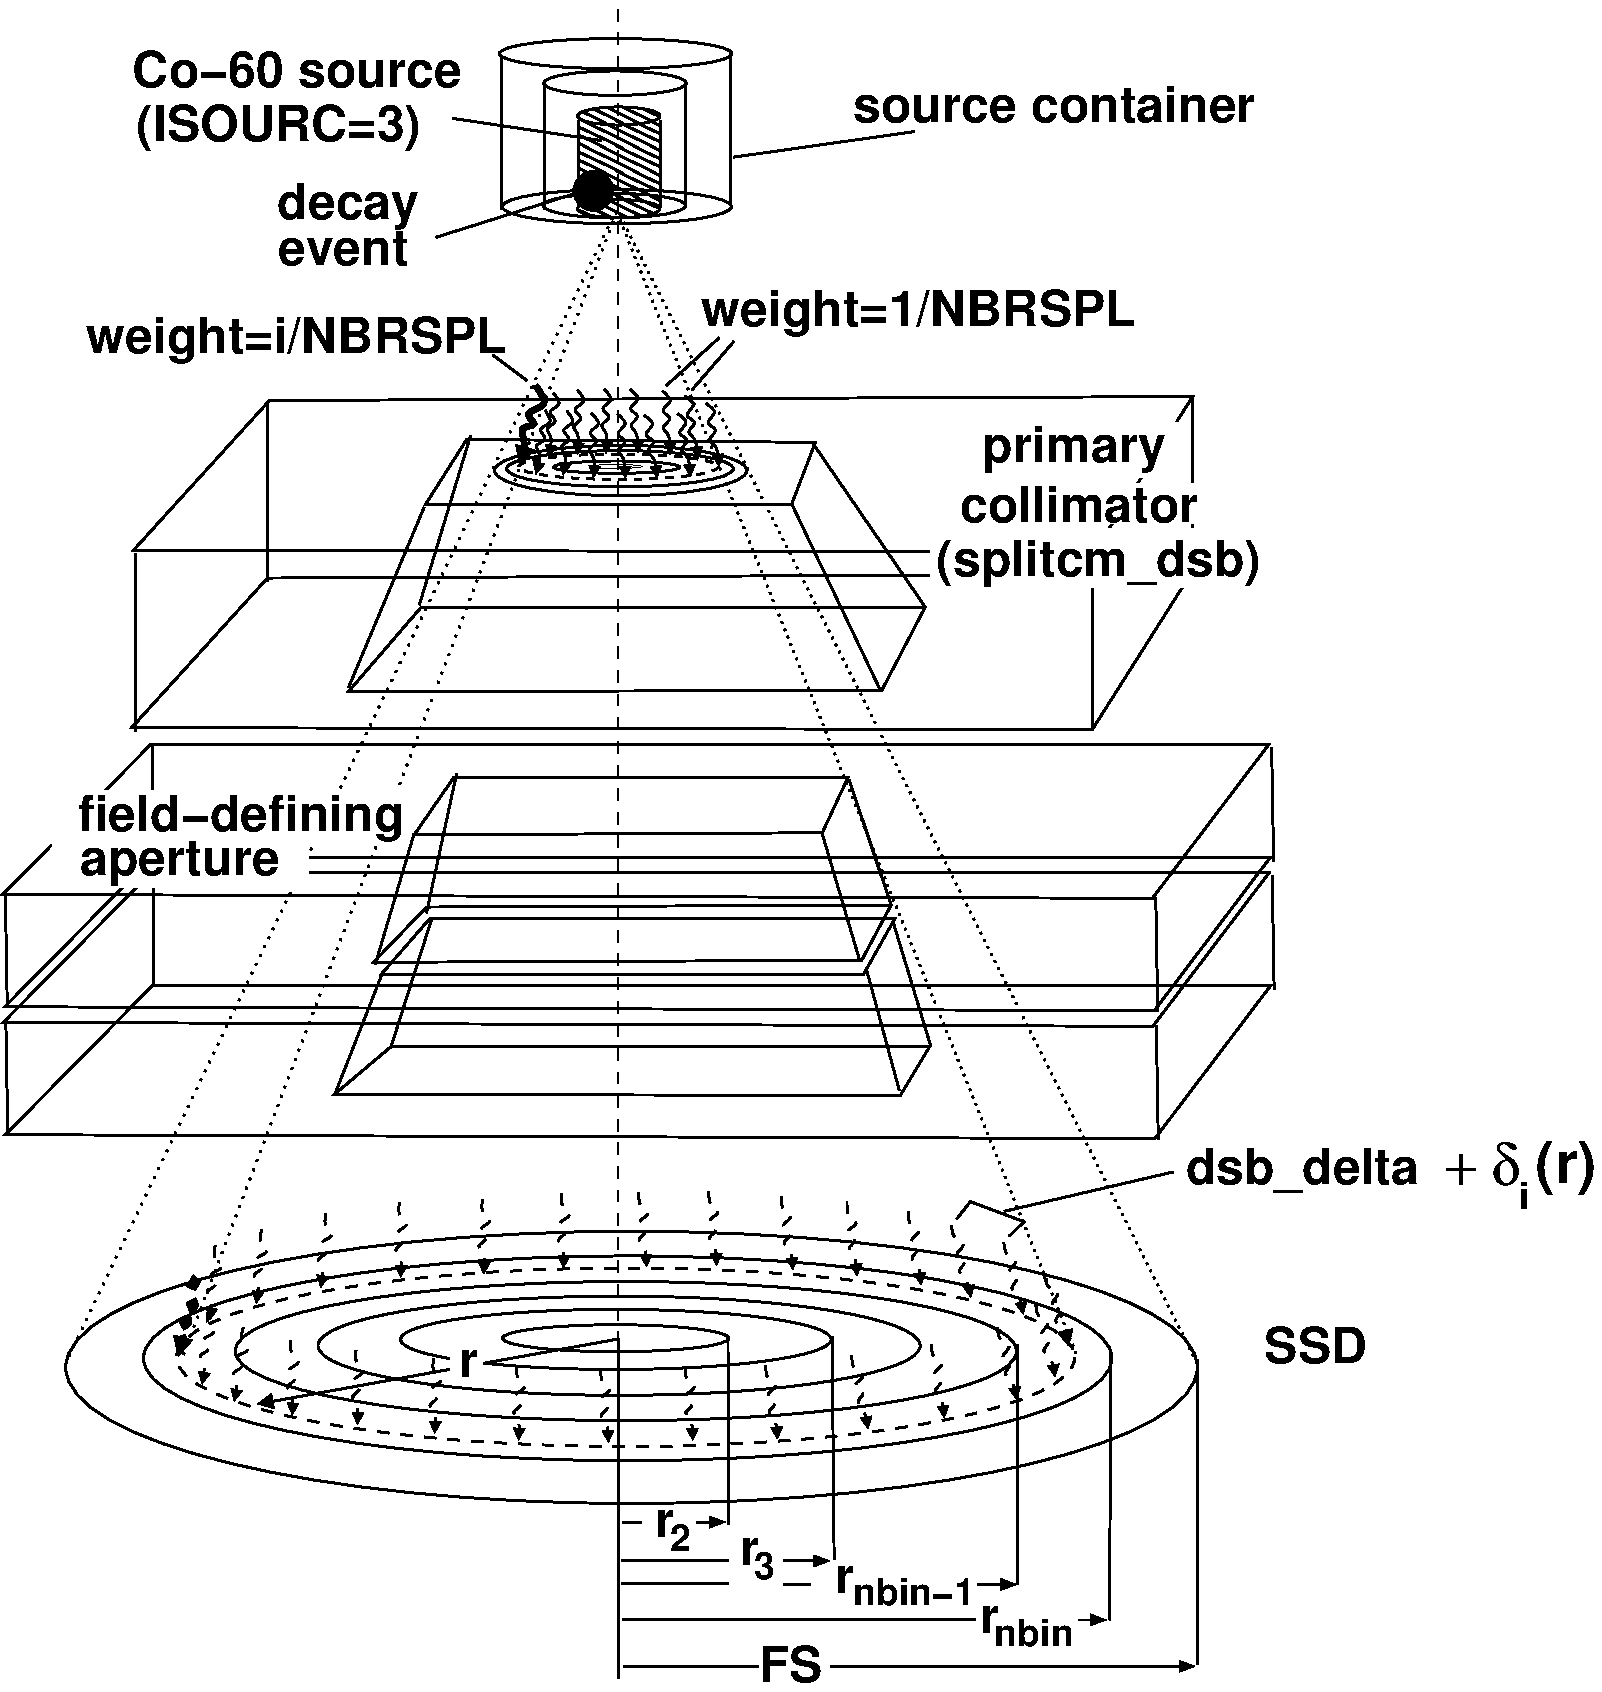
\includegraphics[width=9cm]{figures/dsb}
\end{center}
\caption[Schematic of DSB]
{A schematic of directional source biasing (DSB) in a Co-60 treatment head simulation.
The splitting field is
defined by the user inputs, {\tt FS} and
{\tt SSD} and contains the treatment field.  If there is radial symmetry
above CM number {\tt splitcm\_dsb}, the number of primary photons tracked in
this region can be reduced by dividing the splitting field into {\tt nbin} radial bins.
The number of split primary photons directed into bin i, defined by minimum radius, r$_i$, is
reduced by a factor of i and the weight of each photon is i/{\tt NBRSPL}.  Upon
entering {\tt splitcm\_dsb}, photons are split i times and radially redistributed about the
beam central axis, and their weight is decreased by a factor of i to become 1/{\tt NBRSPL}.
The individual r$_i$ are determined by the user input, {\tt dsb\_delta}, defining
the minimum linear distance between radially redistributed photons ({\em i.e.} for
photons directed exactly at r$_i$).}
\label{dsb_fig}
\end{figure}

\index{directional source biasing!dsb\_delta}
Since {\tt dsb\_delta} defines the minimum linear distance, projected to {\tt SSD}, between split, radially-redistributed photons, the actual linear distance between redistributed photons directed towards radius, r, in bin i is
{\tt dsb\_delta}+$\delta_i(r)$, where $\delta_i(r)$ increases linearly with r from 0 at r=r$_i$ to
$\alpha_{i,max}${\tt dsb\_delta}, with $\alpha_{i,max}<$1, as r$\rightarrow$r$_{i+1}$.

\index{directional source biasing!iphat}
In order to avoid having to reevaluate which radial bin a primary photon is directed into every time Russian
Roulette is played on it or any of its higher-order descendents, the internal variable, {\tt iphat}, is used
When {\tt iphat} was originally introduced with directional bremsstrahlung splitting, it took on only values of 0 or 1
depending on whether a particle was thin
or fat.  With DSB, however, {\tt iphat} now takes on values of 1,2,...,{\tt nbin},{\tt NBRSPL}.
Above {\tt splitcm\_dsb}, {\tt iphat} keeps an instantaneous record of what radial bin a particle (or its descendent)
is directed into ({\tt iphat}$\leq${\tt nbin}) or, if set to {\tt NBRSPL}, indicates that the particle is fat.
Below the top of {\tt splitcm\_dsb}, {\tt iphat} will be either 1, indicating a thin particle, or {\tt NBRSPL}, indicating a fat particle.  This redefinition of {\tt iphat} allows quick calculation of Russian Roulette survival
probabilities ({\em i.e.} 1/{\tt iphat}).

The actual CPU time saved by reducing the number of photons tracked in the radially symmetric portion of
the treatment head as described above depends on the design of the treatment head.  If only a small portion
of the head has radial symmetry, then the CPU time saved will be only a fraction of the overall efficiency
improvement due to DSB.

\index{directional source biasing!electron splitting}
\index{directional source biasing!electron contaminant dose}
If you are interested in contaminant electrons with DSB then you must make use of
the electron splitting scheme implemented in directional bremsstrahlung splitting.  Typical electron splitting
inputs for a Co-60 treatment head simulation using DSB will be different from those for a megvoltage
photon beam using directional bremsstrahlung splitting, and these differences are described in more detail near
the beginning of this section.

\index{directional source biasing!augmented range rejection}
If electron splitting is turned on, then DSB can also make use of directional bremsstrahlung splitting's augmented range rejection scheme (see Section~\ref{dbssect} above).  In this scheme, if a non-fat charged particle cannot make it to
the next region boundary with energy $>$ {\tt ECUT}, then it is subject to Russian Roulette, with survival
probability {\tt iphat}/{\tt NBRSPL}, regardless of whether or not its energy is $<$ the range rejection cutoff
energy, {\tt ESAVE} (see Section~\ref{RR}).  If the particle is not eliminated in this way, then
it is subject to standard range rejection as described in Section~\ref{RR}.

\index{directional source biasing!performance and parameter selection}
\paragraph{DSB performance and parameter selection}\mbox{}\\

Figure~\ref{dsb_deff_fig} below shows the relative efficiency of all doses $>$ 0.5D$_{max}$ calculated in
a water phantom (0.5 cm $\times$ 0.5 cm $\times$ 0.5 cm voxels)  using a BEAMnrc simulation of a
typical Co-60
treatment head (10 cm $\times$ 10 cm field) as a source as a function of the photon
splitting number, {\tt NBRSPL}, selected in DSB.  The Co-60 treatment head model is the same as that
simulated by Mora et al\cite{Mo99} in 1999.  Efficiency is expressed relative
to the efficiency obtained with no variance reduction.  The dotted line shows the maximum efficiency
that can be obtained without DSB using varying values of {\tt ECUT} in the treatment head, with some loss of
accuracy.  Electron contaminant dose is included.

\begin{figure}[htbp]
\begin{center}
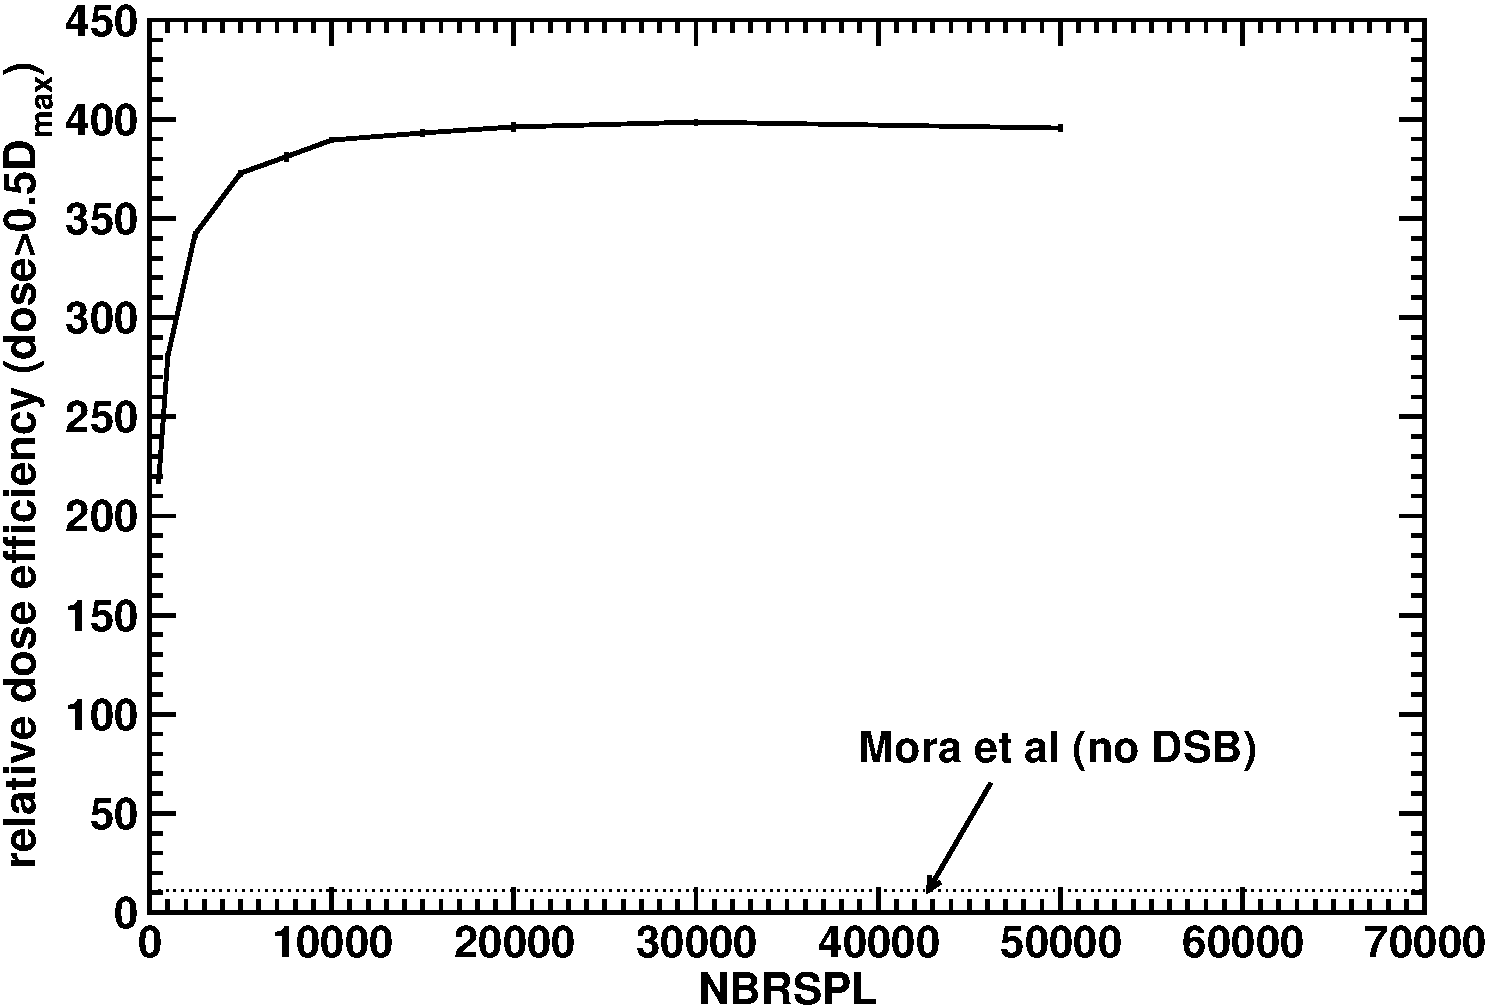
\includegraphics[width=10cm]{figures/dsb_deff_vs_nbrspl_espl}
\end{center}
\caption[Performance of DSB]
{Efficiency of dose calculation in a water phantom (0.5 cm $\times$ 0.5 cm $\times$ 0.5 cm voxels) using
a Co-60 treatment head simulation (10 cm $\times$ 10 cm field) as a source as a
function of DSB photon splitting number, {\tt NBRSPL}.  Efficiency is evaluated for all doses $>$ 0.5D$_{max}$.
Efficiency is relative to that with no variance reduction.  The dotted line shows the maximum efficiency
that can be achieved by varying {\tt ECUT} in the treatment head, with some loss in accuracy.  Electron
contamination is included.}
\label{dsb_deff_fig}
\end{figure}

\index{directional source biasing!selecting optimum splitting no.}
Efficiency with DSB is optimized for {\tt NBRSPL} $\sim$20,000 where it is a factor of $\sim$400 greater than that
with no variance reduction and a factor of $\sim$40 greater than what can be achieved by varying {\tt ECUT}
in the treatment head.  Efficiency does not show significant variation for {\tt NBRSPL} $>$ 20,000.  Therefore,
setting {\tt NBRSPL}=20,000 should be sufficient for typical Co-60 treatment head simulations.

\index{directional source biasing!selecting optimum dsb\_delta}
Efficiency has also been studied as a function of the DSB parameter, {\tt dsb\_delta}, the minimum linear
distance, projected to {\tt SSD}, of radially redistributed photons when they are split upon entering {\tt splitcm\_dsb}.  Within the range 1.0 cm $\leq$ {\tt dsb\_delta} $\leq$ 2.5 cm, photon and contaminant electron fluence effiency
was not found to vary significantly.  Thus, a setting of {\tt dsb\_delta}=1.5 cm is suggested.

Note that the time required to obtain 0.1\% dose uncertainty using the simulated Co-60 treatment
head\cite{Mo99} without DSB and using varying {\tt ECUT} to improve efficiency is $\sim$100 hrs on 15 CPUs (1.8 GHz Opteron).  The factor of $\sim$40 improvement in efficiency obtained using DSB means this calculation can be done in
$\sim$2.5 hrs.

Since DSB potentially generates many incident primary photons per decay event (primary history), incident photon data is
stored in an array. A new decay event is simulated only when all of the data in the array has been used.

For more detailed information about DSB, see the directional source biasing paper\cite{Wa15}.

\subsection[BCSE]{Bremsstrahlung Cross Section Enhancement (BCSE)}
\label{BCSE}
\index{BCSE}
\index{variance reduction!BCSE}
\index{x-ray tubes!variance reduction}

The Bremsstrahlung Cross Section Enhancement (BCSE) variance reduction
technique is introduced into BEAMnrc in the Fall of 2007 to improve
the efficiency of simulations that involve x-ray production from
bremsstrahlung targets (e.g. x-ray tubes and clinical linear
accelerators), both in the kilovoltage and megavoltage range. The
technique is discussed in detail in reference\cite{AR07}. This
section of the manual contains a brief description of the technique
and the input variables used to control it.

BCSE is most valuable in low-energy applications where bremsstrahlung
production is rarest, and in 4$\pi$ geometries where DBS is not
applicable. Except for the few restrictions listed in section
\ref{BCSE_restrictions} below, BCSE is compatible with all other
variance reduction techniques already used in BEAMnrc (e.g. range
rejection, UBS and DBS). BCSE can be used alone or in conjunction with
UBS or DBS; however, the largest efficiency gains are achieved when
BCSE is optimally combined with UBS or DBS. For typical simulations of
interest in medical physics, the efficiency gains can be up to five
orders of magnitude over those obtained with analog simulations, and
up to a full order of magnitude over those obtained with optimized
splitting alone.

\subsubsection{BCSE inputs}
\index{BCSE!inputs}

\noindent The input paramters associated with BCSE  are currently passed
to the code using delimiters in the input file (the same way the EGSnrc
{\tt MC transport parameters} are entered). The following is a template
the user should copy to the end of the input file to be able to use
BCSE (make sure there is no space between the equal sign and the text
preceding it).

\noindent {\tt :Start BCSE:}
\index{:Start BCSE:}

\noindent {\tt Use BCSE= ON} (could be {\tt OFF}, internal variable {\tt
USE\_BCSE} is 0 or 1 for {\tt OFF} or {\tt ON}, respectively).
\index{USE\_BCSE}
\index{Use BCSE}

\noindent {\tt Medium to enhance= med} ({\tt med} is the name of
the medium in which to enhance the bremsstrahlung cross
section (internal variable {\tt BCSE\_MEDNAME}).  The medium must exist
in the accelerator, otherwise BCSE will not be done.
\index{BCSE\_MEDNAME}
\index{Medium number to enhance}


\noindent {\tt Enhancement factor= $n_{2}$} ($n_{2}$ is an integer number
representing the factor by which the bremsstrahlung cross section is
enhanced (internal variable {\tt BCSE\_FACTOR}) )
\index{BCSE\_FACTOR}
\index{Enhancement factor}

\noindent {\tt Russian Roulette= ON} (could be {\tt OFF}. If the focus of
the simulation
is on the photons, it is strongly recommended to set Russian Roulette
{\tt ON}. (internal variable {\tt IRRLTT} which is 0 if {\tt OFF} and 2 if
{\tt ON}.))
\index{IRRLTT}

\noindent {\tt :Stop BCSE:}

\subsubsection{Simulation optimization with BCSE}

For maximum efficiency gains, BCSE should be used with either UBS or
DBS. BCSE+UBS is suitable for 4$\pi$-geometry simulations (e.g. use of
miniature x-ray sources in brachytherapy) whereas BCSE+DBS is suitable
for directional geometry simulations (kilovoltage x-ray systems and
megavoltage clinical linear accelerators). When BCSE is used with
either UBS or DBS, the following two steps can be used to optimize the
simulation for production runs.
\index{BCSE!optimization}
\index{BCSE!parameter selection}

\noindent {\bf Step 1:} The user chooses an optimum {\tt BCSE\_FACTOR}
depending on the simulation type. Recommended values of {\tt
BCSE\_FACTOR} are listed in table \ref{table_optima}. Getting the
maximum efficiency gain is not very sensitive to the exact choice of
{\tt BCSE\_FACTOR} because the complementary {\tt NBRSPL} of the
splitting technique should pick up any little difference and get the
efficiency gain very close to its maximum. For justification of this
argument, see reference\cite{AR07}.
\index{BCSE\_FACTOR}

\vspace{0.3cm}
\begin{table}[h]
\caption{Recommended bremsstrahlung cross section enhancement factor
({\tt BCSE\_FACTOR}). \label{table_optima}}
\vspace{-0.5cm}
\begin{center}
\begin{tabular}{|c|c|c|}
\hline
 & & \\
simulation type & incident electron energy range & recommended {\tt BCSE\_FACTOR} \\
 & & \\ \hline
 4$\pi$ geometry (brachytherapy) & kilovoltage range & $\sim$500 \\
x-ray tubes & mammography range & $\sim$500 \\
x-ray tubes & diagnostic range & $\sim$200 \\
x-ray tubes & orthovoltage range & $\sim$100 \\
clinical linear accelerators & megavoltage range & $\sim$20 \\
\hline
\end{tabular}
\end{center}
\end{table}
\vspace{0.3cm}
\index{BCSE\_FACTOR}
\index{x-ray tubes}

\noindent {\bf Step 2:} The user determines the complementary {\tt
NBRSPL} (this applies to both UBS and DBS) by applying Kawrakow's
model from reference\cite{MK06} as follows:

\noindent $\bullet$ Perform a few short runs with {\tt BCSE\_FACTOR}
from step 1, each with a different {\tt NBRSPL} value.
\index{NBRSPL}

\noindent $\bullet$ Calculate the efficiency of each run,
$\varepsilon_{N_{i}} = \frac{1}{T_{i}~s_{i}^{2}}$, where $N_{i}$ is
the splitting number used for run $i$, $T_{i}$ is the simulation CPU
time for run $i$, and $s_{i}^{2}$ is the average statistical variance
on the scored quantity of interest for run $i$.

\noindent $\bullet$ Fit $N_{i}/\varepsilon_{N_{i}}$ versus
$(N_{i}-1)$ to the following quadratic equation:
\begin{equation}
\frac{N_{i}}{\varepsilon_{N_{i}}}~=~A_{0}+A_{1}(N_{i}-1)+A_{2}(N_{i}-1)^{2}
\end{equation}
where $A_{i}, i=0,1,2$ are polynomial coefficients.

\noindent $\bullet$ Calculate the optimum splitting number {\tt
NBRSPL} using {\tt NBRSPL} = $\sqrt{A_{0}/A_{2}}$.

\noindent Production runs then use {\tt BCSE\_FACTOR} from step 1, and
{\tt NBRSPL} from step 2 for maximum simulation efficiency.

\noindent To use BCSE alone (i.e. without UBS or DBS), table
\ref{table_optima} should not be used. Instead, the user should
perform a few short runs with different values of {\tt BCSE\_FACTOR}
(typically much larger than those in table \ref{table_optima}), then
follow the remainder of step 2 above with {\tt BCSE\_FACTOR} replacing
$N_{i}$.

\subsubsection{Restrictions \label{BCSE_restrictions}}
\index{BCSE!restrictions}

The following are restrictions and cautionary remarks that should be
considered when using BCSE.

\noindent $\bullet$ The user can enhance the bremsstrahlung cross
section in one medium only (which may exist in single or multiple
geometric regions). This is not an intrinsic restriction, but a restriction
due to present coding.

\noindent $\bullet$ If more than one geometric region is made of the
same medium (e.g. target and jaws made of tungsten), and the user wants
to use BCSE for one or more of these regions (e.g. target only), the
user needs to: (1) Duplicate the data of the particular medium of
interest in the PEGS4 data file (copy and paste), (2) Assign the
duplicate data set a different medium name, and (3) Use one medium
name for the geometric region(s) where BCSE will be used and the other
material name for the all other geometric regions where BCSE will not
be used.

\noindent $\bullet$ When BCSE is used with UBS, Russian Roulette
cannot be {\tt ON} for one technique and {\tt OFF} for the other. It
must be either {\tt ON} for both or {\tt OFF} for both.

\noindent $\bullet$ BCSE cannot be used if the electron beam incident
on the bremsstrahlung target has variable electron weights.

\noindent $\bullet$ BCSE cannot, at present, be combined with
Directional Source Biasing (DSB).

\subsubsection{Outline of the BCSE algorithm}

\index{BCSE!algorithm}
When BCSE is used {\em without} UBS or DBS, BEAMnrc implements the following
algorithm\cite{AR07}:

\noindent 1. The bremsstrahlung cross section in the medium of
interest, {\tt BCSE\_MEDNAME}, which is typically the bremsstrahlung target in
an x-ray tube or a clinical linear accelerator,
is scaled up by a user-supplied factor {\tt BCSE\_FACTOR}.

\noindent 2. The weight of the resulting bremsstrahlung photons in the
enhanced medium is reduced by a factor {\tt 1/BCSE\_FACTOR}.

\noindent 3. With a probability of {\tt 1/BCSE\_FACTOR}, the energy of
the charged particle is decremented by the amount given to the
bremsstrahlung photon.

\noindent 4. Higher generations of charged particles are created
through photoelectric, Compton and pair production interactions of
first-generation low-weight photons. If the user turns Russian
Roulette {\tt ON}, these higher-order charged particles are eliminated
throughout the full geometry with a survival probability {\tt
1/BCSE\_FACTOR}. The weight of the surviving charged particles is
increased by a factor {\tt BCSE\_FACTOR}. If Russian Roulette is {\tt
OFF}, higher-order charged particles are tracked individually.

\noindent 5. Fat photons would be created through relaxation events
after electron impact ionization (both in the enhanced medium and
elsewhere), through bremsstrahlung events outside the enhanced medium,
and through positron annihilation events. In each of these events, photons
are split,
according to the UBS and DBS algorithms, into {\tt BCSE\_FACTOR}
photons, each with a reduced weight of {\tt 1/BCSE\_FACTOR}.

\noindent When BCSE is used {\em with} UBS or DBS, BEAMnrc implements
an algorithm similar to the one above, except that the splitting
number is made equal to {\tt NBRSPL} only when a bremsstrahlung event
is about to take place in the enhanced medium, and reset to ({\tt
BCSE\_FACTOR $\cdot$ NBRSPL}) for all other aspects of the BCSE and
splitting algorithms. See reference\cite{AR07} for more on the
implementation details.

\bigskip


\section{Phase Space Files}
\label{PSF}
\index{phase space files!description}

This section describes the phase space files output by BEAMnrc and the
utilities available for processing them.

\subsection{Description of Phase Space Files}
\label{DPSF}
A phase space file contains data relating to particle position, direction,
charge, \etc~ for every particle crossing a scoring plane.  Phase space
files can be output for each scoring plane in an accelerator.  The input
parameter \verb+IO_OPT+ controls whether or not phase space files are
created.  For more information on \verb+IO_OPT+ see section~\ref{ioopt}
dealing with this variable below.  \index{IO\_OPT}

\index{readphsp}
\index{phase space files!binary format}
\index{binary format -phase space}
\index{byte order}
\index{byte swapping}
The phase space files are binary files and thus suffer from the problem of
being being one of two types which depend on which machine they were
written on (little-endians and big-endians).  The utility program
\verb+readphsp+ can be used to convert between these formats. Files from
DEC alpha and PC Linux machines have the same byte order as each other and
may be interchanged.  Files from SUNs, SGIs, RS6000s, and HP9000s are the
same and can be interchanged.  We have also slightly compressed the files
to save space.
\index{readphsp}
\index{phase space files!binary format}
\index{binary format -phase space}

\index{MODE}
The first record in a file is different from the others and contains
the following information.
\begin{description}
\item [MODE\_RW] The file mode: it can be either 'MODE0' or 'MODE2' depending
on whether
\verb+ZLAST+ is included in the phase-space parameters.
\item [NPPHSP] The total number of particles in the file.
\index{NPPHSP}
\item [NPHOTPHSP] The total number of photons in the file.
\index{NPHOTPHSP}
\item [EKMAXPHSP] The maximum kinetic energy of the particles stored in
the file.
\item [EKMINPHSPE] The minimum electron kinetic energy (MeV).
\index{EKMINPHSPE}
\item [NINCPHSP] The number of particles incident from the original (non-phase
               space) source used to generate the phase space file.
\index{NINCPHSP}
\end{description}

Where a phase space file is generated by a simulation using a phase space
file as the  source
(\verb+ISOURC+=21), in the output phase space file, \verb+NINCPHSP+,
the equivalent number of particles incident
from the original non-phase space source,  is equal to
\[{\tt NINCPHSP}=
\frac{{\tt IHSTRY+\left(NRCYCL+1\right)\left(NPASS\_ph\_sp+NFAT\_ph\_sp\right)}}
     {{\tt NPPHSP_{source}}}*{\tt NINCPHSP_{source}}
\]
where \verb+IHSTRY+ is the number of histories run,
{\tt NPASS\_ph\_sp} is the number of particles rejected from the source
because they were multiple passers, {\tt NFAT\_ph\_sp} is the number
of fat photons rejected from the source (only if directional bremsstrahlung
is used--see section~\ref{dbssect}), and {\tt NRCYCL} is the number
of times each particle in the source is recycled (see section~\ref{phspsrcsect}).  The value of
\verb+NINCPHSP+ is stored
in any phase space files generated by the phase space source
and is also used to normalize doses and fluences resulting from the phase
space source.
Thus, \verb+NINCPHSP+, doses and fluences are traceable back to
the original source. For example, consider a model of a $^{60}Co$ unit
which is broken into 2 components. In the first part, the source capsule
is modelled and a phase space file created with all the particles
leaving the surface of the capsule.  Here all outputs are normalized
per photon from the $^{60}Co$.  In the second stage, the phase
space file from the first part is used as input to a model of the
collimator system.  Here again the outputs are normalized per photon
from the $^{60}Co$, thus automatically maintaining the
``natural'' normalization.
\index{normalization!of dose and fluence when using ISOURC=21}
\index{dose!normalization when using ISOURC=21}
\index{fluence!normalization when using ISOURC=21}

Each record in a phase space file contains the following information
about a particle (in this order):\\
\verb+LATCH, E, X, Y, U, V, WT, (ZLAST)+\\
where:
\vspace*{-4mm}
\index{LATCH!in phase space}
\index{WT}
\index{ZLAST}
\begin{description}
\item [LATCH] contains the particle charge, IQ, the number of times
the particle has crossed the scoring plane, \verb+NPASS+, and information
\index{NPASS}
which allows the particle's history to be traced (see section~\ref{LATCH}
below).  The value of \verb+LATCH+ in the phase space file is not the
same as that internal to BEAMnrc or other analysis codes
because of the compression used.
\index{LATCH!in phase space}
\item [E] is the particle total energy (kinetic and rest mass, single
precision).  This is set negative if this is the first particle scored
from a new primary (ie from a non-phase space source) history.
\item [X] is the particle X-position (cm)
\item [Y] is the particle Y-position (cm)
\item [U] is the X-direction cosine
\item [V] is the Y-direction cosine
\item [WT] is the particle's weight; WT also carries the
sign of W, the Z-direction cosine
\item [ZLAST] is the Z-position of last interaction for photons and is
the Z-position of where an electron or its ancestor was set in motion by
a photon (i.e. it does not flag the creation site of delta rays. This
variable is in brackets because its inclusion in the phase space file
depends upon the setting of the input variable
\verb+IZLAST+ (see section~\ref{IZLAST} on \verb+IZLAST+).  If a
particle does not interact, ZLAST is the value it had as it entered the
simulation ({\tt ZIN}).
\index{ZLAST} \index{IZLAST}
\index{phase space files!description}

\end{description}

The magnitude of the Z-direction cosine, W, is determined from
W~=~$\sqrt{1-(U^2+V^2)}$. The particle's charge is stored in bits 29/30
of \verb+LATCH+ and recovered when read in.

\index{energy!negative used as marker in phase space sources}
\index{phase space files!as source}
We set {\tt E} negative for the first particle scored by each new
primary (non-phase space) history in order to be able to group scored
quantities (energy deposited, fluence, etc) according to primary history
when a phase space file is used as a source.  This is necessary to
account for correlations between incident particles and ensures a
correct estimate of the uncertainty on the scored quantities~\cite{Wa02a}.
The negative {\tt E} marker is propagated to phase space files generated
using a phase space source, so that, even in these second-generation
files, particles can be grouped according to the original primary
histories.  When a negative {\tt E} is read from a phase space source,
the primary history counter is incremented and the particle's energy
is set to $|${\tt E}$|$.

\index{phase space files!using old files as source}
If you are using an old phase space file without negative
{\tt E} markers as a source, scored quantities will be grouped according
to incident particle instead of primary history.  BEAMnrc will output
a warning that uncertainties may be underestimated because correlations
between incident particles cannot be accounted for.  However, we have
shown that in most cases the underestimates in uncertainty caused by
not taking correlations into account are
not significant~\cite{Wa02a}.

When BEAMnrc writes a phase space file, it opens the file using\\
\verb+ACCESS = 'direct', FORM = 'unformatted', RECL = 'length'+.\\
The \verb+FORM='unformatted'+ statement ensures that
the file will be stored in a
compressed format, requiring less disk space.  The record length,
'length', depends on the machine being used to run BEAMnrc; on SUN
stations and Linux PC's, 'length' is the number of bytes/record
(28 or 32 [with {\tt ZLAST}]);
on SGI and DEC alpha
machines, 'length' is the number of variables stored in a
record (7 or 8 [with {\tt ZLAST}]).   Internally `length' is determined as
7*\verb+$RECL_FACTOR+ or 8*\verb+$RECL_FACTOR+ (with {\tt ZLAST}),
where the value of the macro is 1 or 4 and is defined in
\verb+$HEN_HOUSE/lib/${my_machine}/machine.mortran+.
\index{machine.mortran}

\index{ZLAST}
\index{MODE}
\index{\$RECL\_FACTOR}
The format of phase space files opened with \\
\verb+ACCESS = 'direct',  FORM = 'unformatted'+ is called
'MODE0' if
\verb+ZLAST+ is not
scored and 'MODE2' if
\verb+ZLAST+ is scored.  The 'MODE0' or 'MODE2'
designation appears in the first record of a phase space file along
with the total number of particles contained in the file, the number
of photons, maximum kinetic energy of any particle in the file,
minimum kinetic energy of electrons, and the number of particles incident
from the original source.

An older version of BEAM opened files in compressed format but with\\
\verb+ACCESS='sequential'+.  These older files are designated 'MODE1' without
\verb+ZLAST+ and\\ 'MODE3' with \verb+ZLAST+.  The current version of BEAM requires
conversion of files in the older format to access='direct' format before adding
new phase space data to them.  The \verb+readphsp+ program described below
performs this conversion.

\index{.egsphsp1}
Phase space files have extension \verb+.egsphsp#+ where \verb+#+
is the number of the scoring plane in the accelerator.  By default, the
maximum number of scoring planes is 3, but this can be adjusted as
described in section~\ref{ctd}.

\index{phsp\_macros.mortran}
\index{phase space files!reading, writing}
BEAMnrc makes use of macros stored in
{\tt \$HEN\_HOUSE/utils/phsp\_macros.mortran} to read and
write the phase space files.  Currently, we have optimised the
writing macros to store up and write 1000 particles at a time.  This has
been found to save network time.  Certainly, there are other read/write
optimisations that could be made, however, in a normal accelerator simulation,
only a small fraction of the simulation time is taken up reading from and
writing to phase space files.
The source for these macros is kept separately so that users may
utilise them in their own codes to read or write phase space files.
The same macros are used uniformly throughout the
BEAMnrc system (DOSXYZnrc, BEAMDP, BEAMnrc \etc).
\index{phsp\_macros.mortran}

\subsection{Maximum size of Phase Space Files}
\index{Phase space files!maximum size}
Note that the variable written to header storing the number of particles
in a phase space file, {\tt NPPHSP}, is a 4-byte integer.  This puts a
practical limit to the number of particles that can be stored in
a phase space file of 2$^{31}$-1.  To put this into perspective, a file
without {\tt ZLAST} containing this many particles would be $\sim$60 GBytes,
and a file storing {\tt ZLAST} would be $\sim$69 GBytes.  It is theoretically
possible to remove this limit on phase space file size and either:
\begin{itemize}
\item not have the number of particles in the file reflected in {\tt NPPHSP} in
the header, which will require other modifications to codes using this phase space
file as a source since, currently, BEAMnrc (and other EGSnrc user codes) compares
the number of histories run to {\tt NPPHSP} in order to determine whether the
source needs to be restarted from the beginning or not, or
\item redefine {\tt NPPSHP} as a 4-byte real variable, in the process losing
precision in terms of the actual number of particles stored in the file.
\end{itemize}

Given these trade-offs, and short of redefining the format of the
phase space header, we prefer to keep 2$^{31}$-1 as a hard limit and suggest that if you require
more data in a phase space source that you run a BEAM shared library source
instead (see Section~\ref{sharedlibsect}).

\subsection{Directory for Phase Space Output}
\label{phspoutdirsect}
\index{phase space files!output directory}

By default, phase space files from an accelerator simulation are
written to the directory
{\tt \$EGS\_HOME/BEAM\_myaccel} ({\em i.e.} the accelerator
directory).  However, you do have the option to output
phase space files to a different directory.
This is particularly useful if you are writing
large phase space files and, due to disk space limitations, you
want to write them directly to a {\tt /temp} storage directory on
another machine (provided it is connected
with NFS to the machine(s) you are running on).

BEAMnrc provides two different ways to change the phase space output
directory:

\begin{description}
\item
\index{beamnrc\_user\_macros.mortran}
In the {\tt \$OMEGA\_HOME/beamnrc/beamnrc\_user\_macros.mortran} file, you can
redefine the macro {\tt \$DIRECTORY-FOR-PHSP}, which
is currently set to {\tt \$EGS\_HOME/BEAM\_myaccel}, to
to be the directory you want to write phase space files to.  Note that you
must provide the full directory path in single quotes
({\em i.e.} {\tt '/full path to directory'}).  An example is given in
the {\tt beamnrc\_user\_macros.mortran} file.  Once you have made this
change, you must recompile your accelerator to put it into effect.

\item
\index{PHSP\_OUTDIR}
BEAMnrc also has a built-in custom user input that you can use
to set the variable {\tt PHSP\_OUTDIR}, which redefines the output
directory for phase space files.  The input line is:\\
{\tt Phsp output directory= /full path to phase space output directory}\\
This must appear in the accelerator {\tt .egsinp} file
in the custom input block delimited by
{\tt :Start user inputs:} and {\tt :Stop user inputs:}.
The custom input block can be placed either
just before or just after the EGSnrc transport parameters
(see Section~\ref{custom_inputs} for more about custom
inputs).  If the input is left blank or
omitted entirely, then the phase space output directory defaults
to that defined by the
{\tt \$DIRECTORY-FOR-PHSP} macro in {\tt beamnrc\_user\_macros.mortran} (see
above).  Note that the GUI does not give
you access to this input.  This method of changing the output
directory for phase space files has the advantage that the accelerator
does not need to be recompiled whenever the output directory is
changed and that different input files for the same accelerator
can specify different phase space output directories.

\end{description}

\subsection{IAEA-format phase space data}
\index{IAEA phase space data}
\label{iaeasect}

Provided that the user's system has a working C++ compiler (determined
automatically on BEAMnrc installation), then BEAMnrc has the capability to
read/write phase space data in IAEA format.  This allows the user to
\index{IAEA phase space database}
add to or make use of data from the IAEA's online accelerator phase space
database at:\\
\htmladdnormallink{www-nds.iaea.org/phsp/phsp.htmlx}{http://www-nds.iaea.org/phsp/phsp.htmlx}

\subsubsection{IAEA format}
\index{IAEA format}
A complete description of the IAEA phase space format is given in IAEA's
technical report INDC(NDS)-0484\cite{CJ05}, which is available from the online
phase space database indicated above.  The format is quite flexible in
terms of the amount of data that is stored.  This section gives a brief
description of the IAEA data that is output and read by BEAMnrc.

\index{IAEA phase space!naming scheme}
\index{{\tt .IAEAheader}}
\index{{\tt .IAEAphsp}}
Phase space data in IAEA format is contained in 2 files: the data file
(with extension {\tt .IAEAphsp}) and
the header file (with extension {\tt .IAEAheader}).  IAEA-format header and
phase space data files output
by BEAMnrc have the names {\tt inputfile.\#.IAEAheader} and
{\tt inputfile.\#.IAEAphsp}, where \# is the scoring plane number.

\index{IAEA header file!contents}
The IAEA header file output by BEAMnrc contains the following data:\\
\begin{description}
\index{{\tt \$CHECKSUM}}
\item {\tt \$CHECKSUM}: The size of the {\tt .IAEAphsp} in bytes.  This is
used when opening an IAEA (to use it as a source or to add more data to it) to make
sure that there are no errors in the file.
\index{{\tt \$RECORD\_CONTENTS}}
\item {\tt \$RECORD\_CONTENTS}: A block indicating the data that is stored in
the {\tt .IAEAphsp} file.  A ``1'' beside a variable indicates that this is stored
in the {\tt .IAEAphsp} file.  This block also indicates how many extra long integers
and extra floating point variables are stored.  In the case of BEAMnrc, two extra long integers,
{\tt LATCH} and the number of primary histories between this particle and the last
particle scored, are always stored.  In addition, if the input {\tt IZLAST=1}
(See Section~\ref{IZLAST}) then {\tt ZLAST}, the Z of the last interaction site for
photons and the creation site for secondary charged particles, is stored as an
extra floating point variable.
\index{{\tt \$RECORD\_CONSTANT}}
\item {\tt \$RECORD\_CONSTANT}: Values which are set to a constant value.  In the case of
an IAEA file written by BEAMnrc, the Z of the scoring plane is stored here (note that this information is not
available in a standard BEAMnrc phase space file).
\index{{\tt \$RECORD\_LENGTH}}
\item {\tt \$RECORD\_LENGTH}: The length of a phase space record in bytes.
\index{{\tt \$BYTE\_ORDER}}
\item {\tt \$BYTE\_ORDER}: ``1234'' for little endian machines, ``4321'' for big
endian machines.
\index{{\tt \$ORIG\_HISTORIES}}
\item {\tt \$ORIG\_HISTORIES}: No. of primary histories used to generate the phase space data.
\index{{\tt \$PARTICLES}}
\item {\tt \$PARTICLES}: Total no. of particles represented in phase space data.
\index{{\tt \$PHOTONS}}
\item {\tt \$PHOTONS}: No. of photons represented in phase space data.
\index{{\tt \$STATISTICAL\_INFORMATION\_PARTICLES}}
\item {\tt \$STATISTICAL\_INFORMATION\_PARTICLES}: Total weight, min. weight, max. weight, average total energy, min. total energy and max. total energy for each particle type
\index{{\tt \$STATISTICAL\_INFORMATION\_GEOMETRY}}
\item {\tt \$STATISTICAL\_INFORMATION\_GEOMETRY}: min. and max. X and Y of all particles scored.
\end{description}
There are other fields in the header but they are not currently used by BEAMnrc.

\index{IAEA phase space data file!contents}
The phase space data file ({\tt .IAEAphsp}) output by BEAMnrc consists of a record of data for each particle
scored, where a record consists of:
\begin{description}
\index{{\tt type}}
\item {\tt type}: particle type and sign of Z-direction cosine, {\tt W} ({\tt CHAR*1})
\index{{\tt E}}
\item {\tt E}: total energy of the particle ({\tt REAL*4}).  If this is the first particle scored
from a primary history, then, similar to standard BEAMnrc format phase space data, {\tt E} is set negative.
\index{{\tt X}}
\item {\tt X}: X position of the particle ({\tt REAL*4})
\index{{\tt Y}}
\item {\tt Y}: Y position of the particle ({\tt REAL*4})
\index{{\tt U}}
\item {\tt U}: X-direction cosine ({\tt REAL*4})
\index{{\tt V}}
\item {\tt V}: Y-direction cosine ({\tt REAL*4})
\index{{\tt WT}}
\item {\tt WT}: statistical weight of the particle ({\tt REAL*4})
\index{{\tt LATCH}}
\item {\tt LATCH}: value of {\tt LATCH} variable ({\tt INTEGER*4})
\index{{\tt ZLAST}}
\item {\tt ZLAST}: Z of last interaction site of photons or site of creation of secondary
charged particles ({\tt REAL*4}).  This is only output if the input variable {\tt IZLAST=1}
(See Section~\ref{IZLAST}).
\item {\tt MU}: Fractional monitor unit index associated with the particle
({\tt REAL*4}).  {\tt MU} is a number on $[$0,1$]$ chosen at the beginning of each primary history and
used to determine the opening coordinates (field) for synchronized component modules (CMs).
It is scored automatically if there is/are one or more synchronized CMs with time-varying opening
coordinates in the accelerator.  Scoring of {\tt MU} allows
synchronization between the simulation generating the file and any downstream simulations,
also having synchronized CMs, that use the file as a source.  See Section~\ref{CMs} for more information
about synchronized CMs.
\end{description}
Thus, each record is 29 bytes long without {\tt ZLAST} and 33 bytes long if {\tt ZLAST} or {\tt MU} is
output, and 37 bytes if both {\tt ZLAST} and {\tt MU} are output.

Similar to standard BEAMnrc phase space files, a negative energy ({\tt E}) marker is used
to indicate the first particle scored from a new primary history.  This allows quantities
scored (dose, fluence, etc) by correlated particles to be grouped for statistical
analysis when the IAEA phase space file is used as a source.  On reading a negative
energy value, the primary history counter in BEAMnrc is incremented by one, and {\tt E} is set
to its absolute value.

\index{{\tt LATCH}}
Note that, unlike standard BEAMnrc phase space files, {\tt LATCH} is not modified to
\index{{\tt NPASS}}
carry the particle charge and {\tt NPASS} before being written to the phase space file.
\index{{\tt type}}
The charge is stored in {\tt type} and if this particle has already crossed the
scoring plane ({\tt NPASS=1}) then it is simply not written to the file.

\index{IAEA format!writing}
\subsubsection{Writing IAEA phase space data}

By setting the input variable {\tt IO\_OPT=4} (See Section~\ref{ioopt}) you will
output the IAEA phase space data and header files at each scoring plane.

\index{IAEA format!reading}
\subsubsection{Reading IAEA phase space data}

\index{{\tt ISOURC=21}}
If you are using IAEA-format space data as a source ({\em i.e.} {\tt ISOURC=21}.
See Section~\ref{phspsrcsect} above.) then you must specify the full name of the
phase space data ({\tt .IAEAphsp}) file.  BEAMnrc will automatically detect the
{\tt .IAEAphsp} extension and read the data in IAEA-format (with an output message
indicating this to the user).  Note that the header file is assumed to be in the
same directory as the phase space data file.

As with BEAMnrc format phase space sources, the Z-direction cosine, {\tt W} is
calculated from $\sqrt{{\tt U}^2+{\tt V}^2}$.  The sign of {\tt type} is then
applied to {\tt W}.  On reading a negative
energy value, the primary history counter in BEAMnrc is incremented by one, and {\tt E} is set
to its absolute value before being used in a simulation.

Note that BEAMnrc automatically handles 3-D IAEA format phase space sources in which the (X,Y,Z) position
of each particle is stored and 4-D phase space data in which fractional monitor unit index ({\tt MU}) is stored.
In terms of 3-D phase space data, there are restrictions on which component modules the source can
be incident within.  See section~\ref{phspsrcsect} above for more details.

\subsection{readphsp}
\label{readphspsect}
\index{readphsp}
There are several programs and routines in place for processing phase
space files.  One of the most basic of these is the program \verb+readphsp+
located on \verb+$OMEGA_HOME/progs/readphsp+.
\verb+readphsp+ is invoked by:
\begin{verbatim}
readphsp inputfile outputfile
\end{verbatim}
where \verb+inputfile+ includes the \verb+.egsphsp#+ extension and
is the name of the phase space file to be converted, and
\verb+outputfile+ is the name of the file which will contain the
converted data (and must also include any extension you want
to add).
Note that {\tt readphsp} retains compatibility with phase space files having
{\tt .egs4phsp\#} extensions generated by EGS4 versions of BEAM.

\verb+readphsp+ gives the user various file conversion options (\eg\
from direct access mode to sequential access mode).  It can also convert
\index{PAW}
phase space files into a format readable by the CERN program PAW provided
that the necessary libraries are present (see below).

\index{byte swapping}
\index{swapping bytes}
\verb+readphsp+ can be used as a byte swapping tool so that phase
space files generated on another type of machine become compatible with
the type of machine that \verb+readphsp+ is being run on.

The \verb+readphsp+ program also allows selection of a particular charge
from a phase space file, or a subset of a file can be extracted.

\index{phase space files!binary format}
\index{binary format -phase space}
Before converting phase space files \verb+readphsp+ prints a summary of
the file contents.  If this is nonsense, then very likely the file has
the wrong binary format  (\ie\ was generated on a machine which uses a
different binary format). The user should use the option of
\verb+readphsp+ to swap the bytes of the phase space data to make it
compatible with the current machine before otherwise converting the phase
space data to its new form.  When using  \verb+readphsp+ for byte
swapping, the name of the output file can be the same as that of the input
file however the swapped data will overwrite the original data.
\index{readphsp}
\index{phase space files!readphsp}
\index{phase space files}
\index{phase space files!binary format}
\index{phase space files!byte swapping}
\index{byte swapping}

Files related to \verb+readphsp+ are on
\verb+$OMEGA_HOME/progs/readphsp+.
\begin{description}
\index{Makefile}
\item [Makefile] Directs compilation of {\tt readphsp}.  Sources
required files such as\\
{\tt \$HEN\_HOUSE/lib/config/machine.macros}
(where {\tt config} is the name of your configuration) for the
\index{record length factor}
record length factor ({\tt \$RECL-FACTOR}) for 4-byte phase space data on your
particular configuration, and
{\tt \$OMEGA\_HOME/beamnrc/phsp\_macros.mortran}
for phase space reading/writing macros that {\tt readphsp} makes use
of.  You must modify {\tt Makefile} if you want to compile
{\tt readphsp} with PAW libraries (see below) so that phase space data can
be converted into PAW format.  Clear instructions for doing this are given
in the {\tt Makefile}.

\item [readphsp.mortran] the \verb+MORTRAN+ source file.

\index{libpawlib.a}
\index{libpacklib.a}
\index{PAW}
\item [libpawlib.a, libpacklib.a (optional)]
Libraries required for the PAW format
conversion.  These are not included with the distribution because they
are proprietary from CERN, but they are available for free from CERN for
those working on medical research.

\item [dummy.f] which is a routine required to compile \verb+readphsp+
when there are no PAW libraries present.

\end{description}

Normally, {\tt readphsp} is compiled as part of the BEAMnrc installation.
However, it can be compiled separately by going into
{\tt \$OMEGA\_HOME/progs/readphsp} and typing {\tt make}.  This will
leave behind the executable, {\tt readphsp*}, in the
{\tt \$HEN\_HOUSE/bin/config} directory.

Note that {\tt readphsp} does not work with IAEA-format phase space data.

\subsection{BEAMDP}
\index{BEAMDP}

Another important program for processing phase space files is the
\verb+BEAMDP+ program.  For more details about running \verb+BEAMDP+
to derive energy, planar fluence, mean energy and angular distributions
from a phase-space file please see the report
``BEAMDP as a General-purpose Utility''\cite{Ma95b}.

%\newpage
\section{Tracking a Particle's History using LATCH}
\index{LATCH}
\label{LATCH}

The \verb+LATCH+ variable, associated with each particle in a simulation, is a
32-bit variable used to track the particle's history. In the input files
there is an opportunity to define a mapping from geometric regions to
bits (\ie\ bit regions)
using the \verb+IREGION_to_BIT+ variable.  Thus, \eg\ it is
possible that bit 5 corresponds to geometric region 3, and more
importantly, one bit, say 3, can correspond to multiple geometric
regions, \eg\ 1,5,8.  Thus, although the JAWS may consist of 6 different
geometric regions, they can all be associated with a single bit or bit
region.  All regions which are not associated with a bit/bit region by the
user are associated with bit region 23 by default.
Each bit is designated as follows:
\index{bit region}
\index{IREGION\_to\_BIT}
\begin{description}

\index{LATCH!bit definitions}
\index{bremsstrahlung!bit 0 flag} \index{bremsstrahlung!testing for}
\index{annihilation!bit 0 flag} \index{annihilation!testing for}
\item [bit 0] Set to 1 if a bremsstrahlung or positron annihilation
event occurs in the history; 0 otherwise(not used for \verb+LATCH_OPTION+ = 1).
\index{LATCH!LATCH\_OPTION}
\item [bit 1-23] Used to record the bit region where a particle has been and/or
has interacted (Note that the bit set for a region is determined by
\verb+IREGION_TO_BIT+ for that region)
\item [bit 24-28] Stores the bit region number (as opposed to geometric
region) in which a secondary particle
is created; if these bits are all 0, the particle is a primary
particle (not for \verb+LATCH_OPTION+ = 1).
\item [bit 29-30] Store the charge of a particle when \verb+LATCH+ is output
to a phase space file (see section~\ref{PSF} on phase space files).
During a simulation, bit 30 is used to identify  a contaminant particle
but this information is not output to the phase space file. Set to 1 if
the particle is a contaminant particle; 0 otherwise. Note that if
\verb+LATCH+ is not inherited (\ie\ when \verb+LATCH_OPTION+ = 1), bit 30
loses its meaning.


\item [bit 31] Set to 1 if a particle has crossed a scoring plane
more than once when \verb+LATCH+ is output to a phase space file
(see section~\ref{PSF} on phase space files above)
\end{description}

For secondary particles, recording the region number in which they were
created in bits 24-28 is equivalent to multiplying the region number by
2$^{24}$, or 16777216.  Thus, to retrieve the region of origin of a
secondary particles, the \verb+LATCH+ value of the particle must be divided by
16777216 (\ie\ taking the value \verb+INT(LATCH/16777216))+.

The user controls the protocol for setting \verb+LATCH+ using the
\verb+LATCH_OPTION+
\index{LATCH!LATCH\_OPTION}
input variable.  The possible settings of
\verb+LATCH_OPTION+ are:
\begin{description}

\item [LATCH\_OPTION = 1 (Non-Inherited LATCH Setting):]
secondaries do not inherit \verb+LATCH+
values from the primaries that created them;
bits 1-23 of a secondary particle carry no information about the
regions its primary parent(s) has(ve) been.  This option must NOT be
used if \verb+ICM_CONTAM+ is non-zero since the \verb+ICM_CONTAM+ option
needs bit 30. \index{ICM\_CONTAM}
\item [LATCH\_OPTION = 2 (Comprehensive LATCH Setting --default):]
\verb+LATCH+ values\\ are passed on to
secondary particles from the primaries that created them; bits 1-23
for a secondary particle include all regions in which the secondary
particle has been plus those in which its ancestors have been
up to the point where the secondary was created;  uses
bits 24-28 to record the bit region
where secondary particles are created and bit 0 to
record whether or not a bremsstrahlung photon was involved in a
\index{LATCH!LATCH\_OPTION}
\index{bremsstrahlung!bit 0 flag} \index{bremsstrahlung!testing for}
particle's history.
\item [LATCH\_OPTION = 3 (Comprehensive LATCH Setting 2):]
similar to 2, but for\\ photons
bits 1-23 record the regions in which the particles have interacted,
rather than simply the regions in which they have been. After a Compton,
pair or photo-electric event, the charged particles, and in the latter
case, also the fluorescent photons, have the bits 1--23 set for the region
in which they are created to treat the case in which they are created
below cutoff in a manner similar to being created above cutoff (where the
bits would be set on the first step).
\end{description}

To clarify further the setting of \verb+LATCH+ bits under various
\verb+LATCH_OPTION+ values, fig~\ref{fig_latch} and table~\ref{table_latch}
\index{LATCH!LATCH\_OPTION}
summarise the situation for a simple photon accelerator.  Two electrons
enter the simulation and produce bremsstrahlung photons in the target,
bit (and geometric) region 1. One photon goes all the way to the scoring
plane without interacting and the second undergoes a pair production
event in the flattening filter (bit region 3). The electron escapes from
the flattening filter an gets to the scoring plane and the positron
annihilates in the flattening filter and one of the resulting 511 keV
photons gets to the scoring plane.  The user has also defined a
contamination scoring plane just above the JAWS ( \ie\
\verb+ITDOSE_ON=1+, \verb+ICM_CONTAM=4+ (just above the JAWS) and
\index{ICM\_CONTAM} \index{IQ\_CONTAM}
\verb+IQ_CONTAM=-1+).

\clearpage

\begin{figure}[H]
\vspace*{-0.3cm}
\begin{center}
\htmlimage{scale=2.0}
\leavevmode
\mbox{}\hspace{0cm}
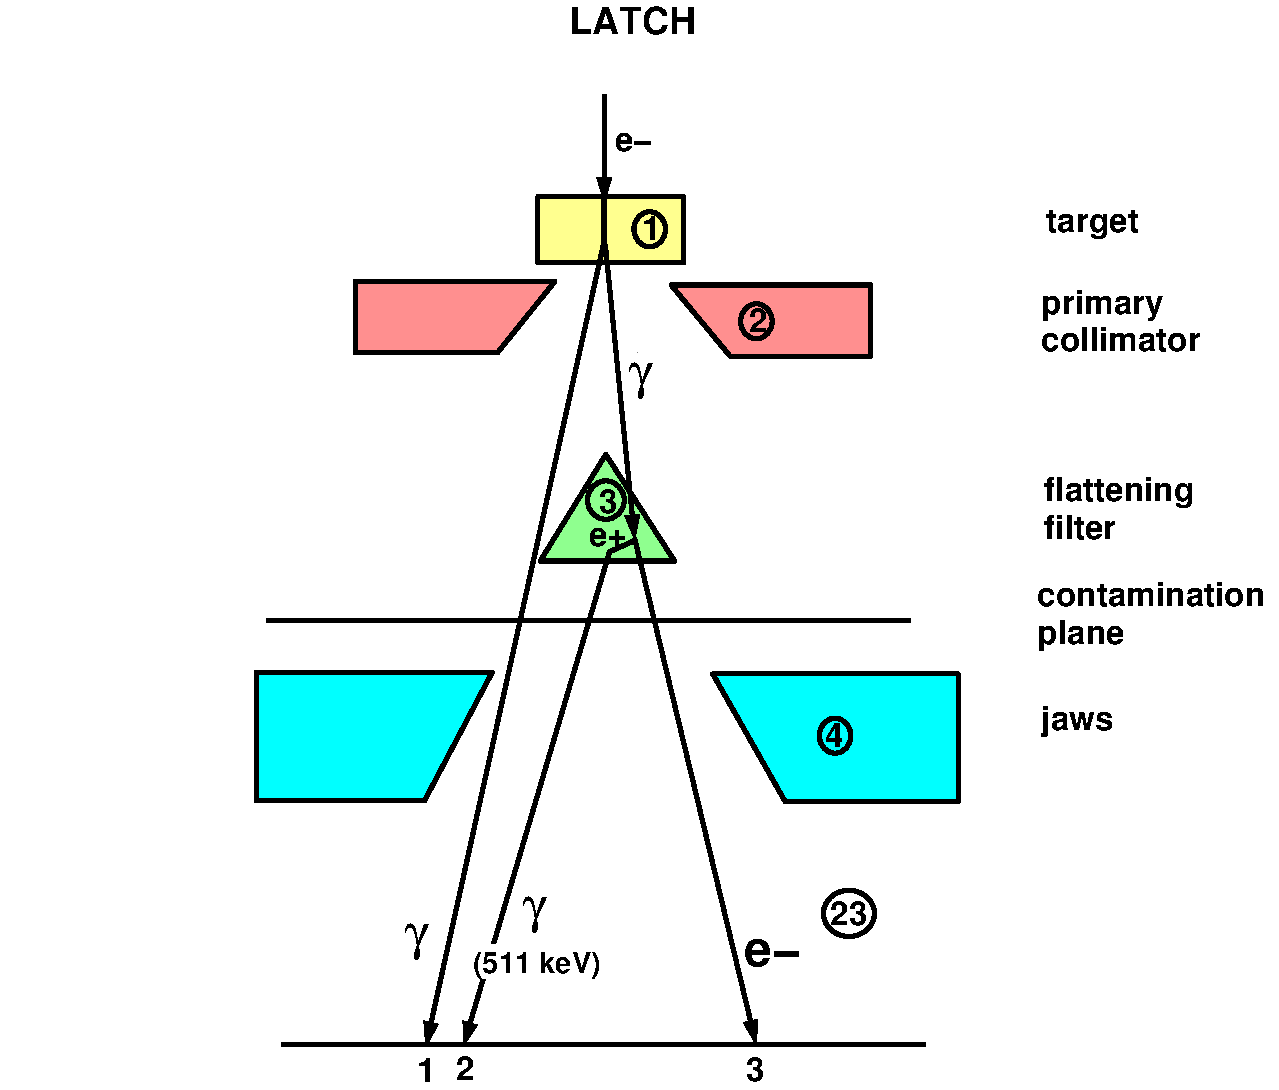
\includegraphics[height=12cm]{figures/latch}
\caption[Example of LATCH settings.]
{Simple photon accelerator model showing 3 particles reaching
the phase space file after 2 electrons are incident.  Contamination is
defined as charged particles crossing the contamination plane.
Table~\ref{table_latch} shows the bit settings in {\tt LATCH} as the particles
reach the scoring plane. The bit region numbers are shown in circles.}
\label{fig_latch}
\end{center}
\end{figure}
\begin{table}[H]
\vspace*{-1cm}
\begin{center}
\caption{Bit settings in LATCH for the simple example shown in
fig~\ref{fig_latch}.}
\label{table_latch}
\begin{tabular}{|r|c|ccccccc|c|c|}
\hline
\multicolumn{1}{|c}{Latch option} &
\multicolumn{1}{|c}{Particle} &
\multicolumn{1}{|c}{Bit 0} &
\multicolumn{1}{c}{1} &
\multicolumn{1}{c}{2} &
\multicolumn{1}{c}{3} &
\multicolumn{1}{c}{4} &
\multicolumn{1}{c}{23} &
\multicolumn{1}{c}{24-28} &
\multicolumn{1}{c|}{30}\\
\hline
1 non-inherited & 1 & 0 & 1 & 0 & 0 & 0 & 1 & 0 & 0\\
~~~             & 2 & 0 & 0 & 0 & 1 & 0 & 1 & 0 & 0\\
~~~~~~~         & 3 & 0 & 0 & 0 & 1 & 0 & 1 & 0 & 0\\
\hline
2 comprehensive & 1 & 1 & 1 & 0 & 0 & 0 & 1 & ``1'' & 0\\
inherited       & 2 & 1 & 1 & 0 & 1 & 0 & 1 & ``3'' & 0\\
where been      & 3 & 1 & 1 & 0 & 1 & 0 & 1 & ``3'' & 1\\
\hline
3 comprehensive & 1 & 1 & 1 & 0 & 0 & 0 & 0 & ``1'' & 0\\
inherited       & 2 & 1 & 1 & 0 & 1 & 0 & 0 & ``3'' & 0\\
where interacted & 3 & 1 & 1 & 0 & 1 & 0 & 1 & ``3'' & 1\\
\hline
\end{tabular}
\end{center}
\end{table}

\clearpage

\section{Calculating Dose Components}
\label{dosecompsect}
\index{dose components}

The ability to trace a particle's history using \verb+LATCH+ also allows doses
to be broken down into their components.  In any dose zone, BEAMnrc is able
to break dose down in 2 ways:
dose from contaminant particles (identified on
the basis of their charge only); or dose including only and/or excluding
only contributions arising from particles with certain user-specified
\verb+LATCH+ bit settings (this is called ``bit filtering'').

\index{ITDOSE\_ON}
The input variables associated with dose component calculations are:
\begin{description}
\item [ITDOSE\_ON] 0 to calculate total dose only (default);
1 to calculate dose components
\end{description}

%The total-stopper dose is calculated automatically if \verb+ITDOSE_ON = 1+.

\index{ICM\_CONTAM}
\index{IQ\_CONTAM}
The following variables are associated with contaminant dose calculation
and are only required if  \verb+ITDOSE_ON = 1+.
\begin{description}
\item [ICM\_CONTAM] contaminant particles are identified upon entering
the top of \verb+CM+ number \verb+ICM_CONTAM+ if 1 $\leq$ \verb+ICM_CONTAM+
$\leq$ total number of \verb+CM+s (previously, this range was restricted to
1 $<$ \verb+ICM_CONTAM+ $\leq$ total number of \verb+CM+s);
if it is set to 0, no contaminant dose will be calculated.
\index{LATCH!LATCH\_OPTION}
\item [IQ\_CONTAM] The charge of the contaminant particles (0 for photons
and 1 for charged particles); all particles
with this charge will be marked as contaminant particles (by setting
\verb+LATCH+ bit  30 of the particles to 1)
upon entering the front of \verb+CM+ number \verb+ICM_CONTAM+.
\end{description}
Contaminant dose is scored in every dose zone.  However it is traced back only
to those particles identified as having contaminant charge upon entering CM
number \verb+ICM_CONTAM+. For example, if \verb+IQ_CONTAM+ = 1, all the charged
particles entering CM number \verb+ICM_CONTAM+ will be marked as contaminant
particles and this mark will be passed onto their descendants via
\verb+LATCH+ bit 30. The dose
contributed by the contaminant particles and their descendants is then scored
as the contaminant dose.  Note that if \verb+LATCH_OPTION = 1+
\verb+LATCH+ values are not transferred to descendants (secondaries),
and contaminant dose calculations will be
meaningless.  Thus, the contaminant dose option is automatically
turned off if \verb+LATCH_OPTION = 1+. Note also that prior to Sept 2002,
contamination was defined as it entered the CM from the front or the back.

The following variables are associated with bit filtering of dose and
are only required if \verb+ITDOSE_ON+ = 1:
\index{ITDOSE\_ON}
\index{bit filters}
\index{LNEXC}
\index{L\_N\_EXC}
\index{LNINC}
\index{L\_N\_INC}
\begin{description}
\item [LNEXC] number of dose components that
exclude contributions from particles with user-specified \verb+LATCH+ bits
set (bit filters). \verb+LNEXC+ = 0 is allowed. \verb+LNEXC <= $MAXIT - 3+
where \verb+$MAXIT+ can be changed from its default value of 12
(as described in section~\ref{ctd}).
\item [L\_N\_EXC(I,31) (I = 1,2,...,LNEXC)] Bit filter for determining
which particles to exclude
from dose component I; each of the LNEXC components requires input of a
separate bit filter; a bit filter consists of a sequence of up to 31
\verb+LATCH+
bit numbers on a single record (range 1-31), separated by commas;
particles with any of the listed bits  set
are excluded from dose component I.
\item [LNINC] number of dose components with contributions only from
particles with user specified bit filters which are a combination of
inclusive and possibly exclusive patterns.  \verb+LNINC+ = 0 is allowed.
\verb+LNINC <= $MAXIT - LNEXC - 3+.
%For example, if the inputs for \verb+L\_N\_EXC(I,31)+ are 2,3,5,0,...,
%then the dose component I will exclude the contributions from the
%particles with any of the LATCH bits 2,3,5 set high (=1)

\item [L\_N\_INC(I,31) (I = 1,2,...,LNINC)] Bit filter for determining
which particles to include in dose component I; each of the LNINC
components requires input of a separate bit filter which consists of 2 groups
of \verb+LATCH+ bit numbers (range 1-31) separated by a 0;
contributions from the particles with any of the \verb+LATCH+ bits in the
first group of \verb+L_N_INC(I,31)+ set and none of those in the second
group set are included in dose component I.

For example, if the inputs for
\verb+L_N_INC(I,31)+ are 2,3,5,0,1,4,0,..., then dose component I will
include the contributions from the particles with {\bf any} of the \verb+LATCH+
bits 2, 3 or 5 set (=1) {\bf and} both \verb+LATCH+ bits 1 and 4 not set (=0);
the status of other \verb+LATCH+ bits will have no effect on this
dose component.
If the inputs are 1,2,3,0,0,...,(equivalently 1,2,3,)
the dose component  will include
the contributions from the particles with any of the \verb+LATCH+
bits 1, 2 or 3
set (=1). Note that no dose will be scored if one inputs 0,2,3,5,0,...


\end{description}

Note that bit 0 of \verb+LATCH+ can not be  used for the above dose
component calculations.


Bit filtering of dose provides a particularly powerful tool for
determining dose contributions.  In view of the information stored in
\verb+LATCH+ (see section above), dose contributions can be separated
according to what regions particles have passed through/interacted in,
whether the particle is a primary or secondary, if the particle is a
secondary then where it was created, whether or not the particle is a
contaminant, and any combination of these.

\index{fat particles}
It should be noted that if directional bremsstrahlung splitting (DBS)
is used in a BEAM simulation then an
additional dose component, the total dose minus the dose due to
fat particles, is automatically output to the {\tt .egslst} and
{\tt .egsplot} files.  see section~\ref{dbssect} for more details.

\section{Other Input Variables}
\label{oiv}

This section provides descriptions of main BEAMnrc input variables not
covered above.

\subsection{IWATCH}
\label{iwatchsect}
\index{IWATCH}
\index{.egslog}

\verb+IWATCH+ controls output to the screen (interactive run) or to the
\verb+.egslog+ file (batch run) during beam execution.  The possible settings
are:
\begin{description}
\item [= 0] (default) On completion of each batch, outputs information about the
batch (eg elapsed time, CPU time, elapsed/CPU time, random number used
to begin batch, \# of random seeds used in the batch, total number of
histories run up to and including the current batch, the total number of
particles scored in the first phase space file)
\index{batches}

\item [= 1] Outputs batch information plus, after every particle
interaction, outputs complete information about the particle(s)
involved (eg interaction type, particle type, position of particle on
stack, particle energy, X-Y-Z position of particle, U-V-W direction
cosines, \verb+LATCH+ value of particle, region \# of particle); also informs
user when a particle is being discarded, when a particle is passing from
one CM to another

\item [= 2] Similar to 1 only complete particle information is output at
every step; also outputs total dose in a region whenever energy is
deposited there

\item [= 3] Similar to 2 only particle and dose information are output
whenever dose is deposited.

\item [= 4] Outputs same information as 0 plus \verb+.egsgph+ and
\verb+egsgeom+
files for graphical representation of the accelerator and particle paths
using \verb+EGS_Windows+\cite{TR99a}.
\index{EGS\_Windows}
\index{.egsgph}
\index{.egsgeom}
\end{description}

\subsection{ISTORE}
\index{ISTORE}

ISTORE controls how BEAMnrc reads and writes the state of the random number
generator (RNG) used in simulations.  The possible
settings of ISTORE are:
\begin{description}
\item [= 0] (default) BEAMnrc stores the state of the RNG for the 1st
history in each batch in the file \verb+.egsrns+
\index{.egsrns}
\item [= 1] BEAMnrc stores the state of the RNG for every history in the
.egsrns file.  The random number state of the current history overwrites
that of the previous history.
\item [= -1] BEAMnrc reads the state of the RNG for the 1st history
from the \verb+.egsrns+ file.  If there was an error during
a history that caused the history to stop, then you can use {\tt ISTORE} = -1
to rerun the problem history, provided that you first stored the state
of the RNG for each history using {\tt ISTORE} = 1.
\index{batches}
\index{.egsrns}
\index{random number generator}
\end{description}

\subsection{IRESTART}
\label{IRESTART}
\index{IRESTART}

IRESTART controls how BEAMnrc treats the current run - either as new or as a
continuation of a previous run. The possible settings of IRESTART are:
\begin{description}
\item [= 0] (default) BEAMnrc initiates a new run, deleting all of the output
files from previous runs of the same name if present
(\verb+.egslog+, \verb+.egslst+, \verb+.egsrns+, \verb+.egsphsp1+,
 \etc).
\index{.egsphsp1}
\index{random number generator}
\index{restart}
\item [= 1] Restart of a previous run; BEAMnrc reads fluence and dose data
from the previous run, the number of histories already run, the time
taken by the previous run, and the state of the random number generator from
the last
batch of the previous run from the \verb+.egsdat+ file; fluence and dose and
their statistics are averaged with those from the previous run; phase
space output is appended to that from the previous run; note that the
number of histories to run in the present run is given by NCASE
but the reported total CPU time and number of histories analysed in the
output include the histories and CPU time from the previous run.
\index{batches}
\item [= 2] BEAMnrc creates the \verb+.egsinp+ file and then exits without
running the simulation.
\item [= 3] BEAMnrc reads dose and fluence data from a previous run in the
\verb+.egsdat+ file, performs statistical analysis
on the data and outputs results to \verb+.egslst+; no simulation is run.
\index{.egsdat}
\item [= 4] For analysis of dose and fluence in a simulation that
has been split up into parallel jobs.  See section~\ref{parallelcalc}
page~\pageref{parallelcalc} below on parallel processing with BEAMnrc
for more details.
\end{description}

\subsection{IO\_OPT}
\index{IO\_OPT}
\label{ioopt}

\verb+IO_OPT+ allows user control of phase space output.  Some aspects of
this variable have already been covered in section~\ref{PSF} on phase space
files.  However, it also controls data analysis of simplified source
models.  The possible settings for
\verb+IO_OPT+ are:
\begin{description}
\item [= 0] (default) Phase space output at each scoring plane
\item [= 1] No phase space output at scoring planes
\item [= 2] No phase space output, but perform data analysis for
simplified source models (see BEAMDP manual).\index{BEAMDP}
\item [= 3] Phase space output for the first 100,000 particles across
each scoring plane and perform data analysis for simplified source
models
\item [= 4] IAEA-format phase space output at each scoring plane
\end{description}

\subsection{IDAT}
\label{IDAT}
\index{IDAT}

\verb+IDAT+ controls output of the \verb+.egsdat+ file, which contains data
from a previous run so that BEAMnrc is able to restart this run
\index{restart}
if required.  The {\tt .egsdat} files from parallel jobs are
required for recombining to obtain the final results (see section~\ref{parallelcalc}).
Possible settings of \verb+IDAT+ are:
\index{.egsdat}

\begin{description}
\item [= 0] (default) Output energy deposited and fluence data,
number of histories completed, elapsed time and the current state of
the random number generator to the
{\tt .egsdat} file upon completion of every batch
\item [= 1] Do not output a {\tt .egsdat} file
\index{batches}
\index{random number generator}
\end{description}

See section~\ref{outputfilessect} for a more complete description of
the {\tt .egsdat} file.

\subsection{IZLAST}
\label{IZLAST}
\index{IZLAST}
\index{ZLAST}

\verb+IZLAST+ controls whether or not {\tt ZLAST}
is recorded in phase space files.
{\tt ZLAST} is the Z-position of last interaction for photons and is
the Z-position of where an electron or its ancestor was set in motion by
a photon (i.e. it does not flag the creation site of delta rays).
The possible settings of \verb+IZLAST+ are:
\begin{description}
\item [= 0] (default) BEAMnrc does not score
\verb+ZLAST+
in phase space files; this means that phase space files are read and
written in compressed ``mode0''
\item [= 1] BEAMnrc scores the Z position of last interaction in phase
space files; phase space files are read and written in compressed ``mode2'';
``mode2'' files are approximately 14\% larger than ``mode0'' files; when
plotting phase space data with paw,
\verb+ZLAST+ replaces the radial position
of a photon (r)
\item [= 2] Same as option 1 and in Addison, BEAMnrc writes the X-Y-Z positions
of the last site of interaction for photons into the \verb+.egsgph+ file.
These last sites of interaction can be viewed in 3-D using
{\tt EGS\_Windows}\cite{TR99a}. {\tt IWATCH}=4
must not be turned on at the same time since it also writes to the
\verb+.egsgph+ file.
\index{EGS\_Windows}

\end{description}
Note that the utility BEAMDP has an option to present graphs of {\tt ZLAST}
in 2-D.

\subsection{NCASE}
\label{ncasesect}
\index{NCASE}
\index{\$NBATCH}
\verb+NCASE+ is the number of histories for this run.  Minimum
value is 100.  Default is 100 if \verb+NCASE+ is set $<$ 100.  The number of
histories per batch is equal to \verb+NCASE+/({\tt \$NBATCH}), where
{\tt \$NBATCH} is the number of output batches.   {\tt \$NBATCH} is
set in the {\tt beamnrc\_user\_macros.mortran} file and is currently
equal to 10.
The total number of histories after this run will be
the sum of \verb+NCASE+ and the number of histories from the previous run.
\index{batches}
\index{NBATCH}

Starting with BEAMnrc, the breaking of the run into batches is for saving
intermediate data and diagnostics. It is no longer associated with
statistical uncertainties.

Starting with BEAM99, {\tt NCASE} and other variables related to the
number of histories,
such as {\tt IHSTRY}, were made {\tt INTEGER*8} variables.  This allows
$>$2x10$^9$ total histories, and is particularly useful for restarts and
parallel runs, where a large number of total histories can be accrued quite
easily.  However, {\tt INTEGER*8} may cause problems for some Fortran compilers.
For a more detailed description of this problem and how to fix it if it does
occur, see section~\ref{knownbugs} on known bugs/restrictions in BEAMnrc.
\index{NCASE! Problems with INTEGER*8}

\subsection{IXXIN, JXXIN}
\label{rngsect}
\index{IXXIN,JXXIN}
\index{random number seeds/pointers}
\index{random number generator}
\index{RANMAR}
\index{RANLUX}

The input values of \verb+IXXIN+ and \verb+JXXIN+
are seeds used to initialize the RANLUX\cite{La94,Ja94} or
RANMAR\cite{MZ91,Ma90a}
random number generator.  Within BEAMnrc, {\tt IXXIN} is limited
to the range 0$<${\tt IXXIN}$\leq$31328 (defaults to 1802), and {\tt JXXIN} has
the range 0$<${\tt JXXIN}$\leq$30081 (defaults to 9373).
These ranges/defaults were originally designed for RANMAR, however, if
you are using RANLUX (the new default) then {\tt IXXIN} is the ``luxury level"
of the random number generator and must be in the range
0$<${\tt IXXIN}$\leq$4, otherwise, it will automatically be set to the
default luxury level of 1 (Note: this means that the BEAM default value
for {\tt IXXIN} of 1802 will ultimately get reset to 1 by RANLUX).  Also,
with RANLUX, the input {\tt JXXIN} can have a maximum value of 1073741824,
however you will have to change the BEAMnrc code to allow this maxium.

Note that \verb+IXXIN+ and \verb+JXXIN+ are only used to initialize
the random number generator, and, during a simulation, they no longer
reflect the values of the seeds that are actually used to generate
the random numbers.
During restarts
({\tt IRESTART} = 1), the state of the random number generator at the end
of the previous run is read from the {\tt .egsdat} file and is used at the
beginning of the restart.  Thus, a restarted run with a total of, eg,
10000+10000 histories should generate results identical to a single run
of the same simulation with 20000 histories.  Also note that
when running parallel
simulations with BEAMnrc (see section~\ref{parallelcalc}), {\tt JXXIN} must have
a different value for each of the individual jobs that make up the simulation.
A property of the random number generators being used is that this simple
change guarantees random number sequences which are independent.

\index{random number generator!changing from RANMAR to RANLUX}
To switch from the default RANMAR to RANLUX in your BEAM code, either go into
\index{beamnrc.spec}
{\tt \$HEN\_HOUSE/specs/beamnrc.spec} and change the line:
\begin{verbatim}
RANDOM = $(EGS_SOURCEDIR)ranmar
\end{verbatim}
to:
\begin{verbatim}
RANDOM = $(EGS_SOURCEDIR)ranlux
\end{verbatim}
(recommended if you plan on using RANLUX as your default random
number generator for all accelerators),
or compile an individual accelerator using the command
\begin{verbatim}
 make RANDOM=$HEN_HOUSE/src/ranlux
\end{verbatim}

\subsection{TIMMAX}
\index{TIMMAX}
\index{CPU time}

\verb+TIMMAX+ is the maximum CPU time in hours allowed for this run.
\verb+TIMMAX+ defaults to 0.99 hours if it is set = 0.
At the end of each batch, an estimate is made of how much time is needed
to complete another batch. If the next batch cannot be completed within
\verb+TIMMAX+ for the current run, then BEAMnrc terminates the run and
analyses the results for the shortened run.  The restart feature (see
section~\ref{IRESTART} on \verb+IRESTART+) can be used to continue the
run if needed and if \verb+IDAT+ (section~\ref{IDAT}) is set to 0 (\ie\ the
{\tt .egsdat} files are created).
Note that the total CPU time
reported for a simulation is the sum of the CPU time so far for this run and
the CPU time from the previous run, but \verb+TIMMAX+ refers to the
present run's time only.
\index{batches}

\subsection{ ECUTIN}
\index{ECUTIN}
\label{ECUTIN}
\index{ECUT}

The electron transport cutoff energy, {\tt ECUT}, defines the minimum
total energy below which electrons are no longer followed.  As soon
as an electron's total energy falls below {\tt ECUT}, its
history is terminated and its energy deposited in the current region.
The time required for a given calculation is strongly dependent on the
value of \verb+ECUT+ and thus it is important to use as high a value
as possible.

The global value of {\tt ECUT} (in MeV) can be defined through either the
{\tt Global ECUT} input in the EGSnrc input parameters
(see Section~\ref{globalecutsect} below) or the BEAMnrc input, {\tt ECUTIN}, with
the greater of the two values used.  If
the {\tt Global ECUT} input from the EGSnrc input parameters is omitted
altogether, then {\tt ECUTIN} is used.

The user can also override the global {\tt ECUT} within individual regions
of component modules (see CM descriptions below) provided that
the value of \verb+ECUT+ for a region is $>$
the global \verb+ECUT+.

Note that \verb+AE+ for the PEGS4 data set used is the lower limit on the
value of \verb+ECUT+ used in a given region.  The selection of \verb+AE+
also requires some care and is discussed in section~\ref{AE}.  \index{AE}
\index{ECUT!rule of thumb}

Selection of \verb+ECUT+ is complex in general and is  dependent on what
is being calculated\cite{Ro84,RB90}.  For therapy beams, \verb+ECUT+
can be quite high since low-energy electrons contribute little to dose
in phantom.  For what we consider detailed work, we have used \verb+ECUT+
= 0.700 MeV but much higher may be possible.  However, if the dose in
the monitor chamber is an important part of the calculation, lower values
of \verb+ECUT+ may be required.

\index{Global ECUT}

As a general rule of thumb for calculations of dose distributions,
\verb+ECUT+ should be chosen so that the electron's range at \verb+ECUT+
is less than about 1/3 of the smallest dimension in a dose scoring region.
This ensures energy is transported and deposited in the correct region
although for electrons which are moving isotropically, this can be a
very conservative requirement.

\subsection{ PCUTIN} \index{PCUTIN} \label{PCUTIN} \index{PCUT}

{\tt PCUT} is the photon equivalent of {\tt ECUT}.  As soon as a
photon's energy falls below {\tt PCUT} transport of the photon is
terminated and its energy is deposited in the current region.

The global value of {\tt PCUT} (in MeV) is defined using either the
{\tt Global PCUT} input in the
EGSnrc input section (see Section~\ref{globalpcutsect} below) or the
BEAMnrc input, {\tt PCUTIN}.  Again, the greater of the two values is
used, and, if the {\tt Global PCUT} input is omitted from the EGSnrc
inputs altogether, then {\tt PCUTIN} is used.
Similar to {\tt ECUT}, the user can override the global value
of \verb+PCUT+ within individual regions of component modules provided
that {\tt PCUT} for that region is $>$ than the global {\tt PCUT}.
\index{Global PCUT}

The exact value of \verb+PCUT+ is not critical in the sense
that low values do not take much more time. A value of 0.01 MeV should
generally be used.

\subsection{ ESTEPIN, SMAX, IDORAY, IFLUOR}
\label{dummyinputs}
\index{ESTEPIN}
\index{SMAX}
\index{IDORAY}
\index{IFLUOR}

These are dummy inputs which used to define the maximum fractional energy
loss per electron step
({\tt ESTEPIN}), the maximum step length ({\tt SMAX}),
a switch for turning on Rayleigh scattering
({\tt IDORAY}), and a switch to turn on K-shell X-ray fluorescence
({\tt IFLUOR}).  Now all of these transport parameters are
handled in the EGSnrc inputs (see section~\ref{egsnrc_inputs}), however,
the dummy inputs are retained for compatibility with older EGS4 BEAM
input files.

\subsection{ ICM\_SPLIT, NSPLIT\_PHOT, NSPLIT\_ELEC}
\label{icmsplit}
\index{ICM\_SPLIT}
\index{NSPLIT\_PHOT}
\index{NSPLIT\_ELEC}

{\tt ICM\_SPLIT} is used to split photons and electrons at an arbitrary
plane within an accelerator.  To use this option, the user sets
{\tt ICM\_SPLIT} equal to the CM \# at the top of which the photons and electrons
are to be split.  When {\tt ICM\_SPLIT}$>$0, then the user must
input {\tt NSPLIT\_PHOT} and {\tt NSPLIT\_ELEC}, the splitting number for
photons
and electrons, respectively, upon entering the CM.  If
{\tt NSPLIT\_PHOT} or {\tt NSPLIT\_ELEC} is $\leq$1, then the relevant
particle type is not split at all.  Once a particle
has been split, the resultant particles carry weight
1/{\tt NSPLIT\_PHOT} or 1/{\tt NSPLIT\_ELEC}.  A particle is only split
upon entering the user-specified CM from the top (\ie\ {\tt W(NP) > 0})
and if it has not been split by this option before.

Splitting at an
arbitrary plane was designed primarily for improving statistics in
dose calculations in a phantom,
in which case particles (usually photons) would be split upon entering a
phantom at the bottom of the accelerator.  Use of this option near the
top of an accelerator may produce undesirable correlations, without much
gain in efficiency.

The {\tt ICM\_SPLIT} option operates in conjunction with any kind of
bremsstrahlung splitting and photon forcing.  In the case where
{\tt ICM\_SPLIT}={\tt NFCMIN} (\ie\ the arbitrary splitting plane corresponds
to the plane at which photon forcing is to begin), the photons are split
BEFORE they are forced to interact.

Currently, if {\tt ICM\_SPLIT}=1, then the
option is turned on, but no splitting will occur.  We  hope to remove this
restriction, but if you wish to split particles in CM 1, you can
get around the problem, by inserting a dummy CM 1 and setting
{\tt ICM\_SPLIT}=2.

\section{EGSnrc inputs}
\label{egsnrc_inputs}
\index{EGSnrc inputs}

The use of EGSnrc to simulate charged particle and photon transport
in BEAMnrc allows the user a greater degree of control over the
transport physics
than was previously available in EGS4 versions of BEAM.  For most
accelerator applications, the default settings in the BEAMnrc code for the EGSnrc
parameters should be adequate (these are not the same as the EGSnrc
standard defaults).   However, there are some cases, such
as low energy applications, in which the user will want to vary
the EGSnrc transport parameters using the EGSnrc inputs.

EGSnrc inputs appear at the end of a BEAMnrc input file using the new
format used with the general purpose user EGSnrc user codes.  The input
occurs between the
delimiters {\tt :start mc transport parameter:} and
{\tt :stop mc transport parameter:}.

In general, EGSnrc inputs must appear in the input file in
the format:\\
{\tt PARAMETER NAME= parameter value}\\
Note that there is a space between the ``='' sign and the parameter value
but not before the ``='' sign.
If you are using the BEAMnrc GUI to set the EGSnrc inputs, then
the above format is written to the input file automatically when you save
the input parameters.

If any or all of the EGSnrc input parameters is missing, then the default
setting will be used. This feature allows BEAM input files to be used
directly with BEAMnrc. A better approach is to read the old BEAM input
file into the {\tt beamnrc\_gui} and then save it since this will explicitly
add the required EGSnrc inputs to the file.

The following sections describe the EGSnrc inputs required in
BEAMnrc.  For more information, see the EGSnrc manual\cite{KR03}. The
actual internal variable name associated with each input appears in brackets.

\subsection{ {\tt Global ECUT} ({\tt ECUT})}
\label{globalecutsect}
\index{Global ECUT}
\index{ECUT}
\index{ECUTIN}
{\tt Global ECUT} defines the global electron cutoff energy ({\tt ECUT})
in MeV.  If {\tt ECUTIN}
in the main
BEAMnrc inputs is $>$ {\tt Global ECUT}, or if {\tt Global ECUT} is
omitted from the EGSnrc input section, then the global value of
{\tt ECUT} is set to {\tt ECUTIN}.  See section~\ref{ECUTIN} for a more
detailed discussion of {\tt ECUT}.

\subsection{ {\tt Global PCUT} ({\tt PCUT})}
\label{globalpcutsect}
\index{Global PCUT}
\index{PCUT}
\index{PCUTIN}
{\tt Global PCUT} defines the global photon cutoff energy ({\tt PCUT})
in MeV.
If {\tt PCUTIN} in the main
BEAMnrc inputs is $>$ {\tt Global PCUT}, or if {\tt Global PCUT} is
missing from the EGSnrc input section, then the global value of
{\tt PCUT} is set to {\tt PCUTIN}.  See section~\ref{PCUTIN} for a more
detailed discussion of {\tt PCUT}.

\subsection{{\tt Global SMAX} ({\tt SMAXIR})}
\index{Global SMAX}
\index{SMAX}
\index{SMAXIR}
{\tt Global SMAX} defines the maximum electron step length in cm.  If the
default EGSnrc electron step electron algorithm (see
section~\ref{essect}) and the exact boundary crossing algorithm are used, then no
restriction on maximum step length is needed.  However, if using
PRESTA-I (the EGS4 standard) as the electron step algorithm or the boundary
crossing algorithm, then
{\tt Global SMAX} must be set to a reasonable value (eg 5 cm) to ensure
proper electron transport in low density materials (air).
{\tt Global SMAX} defaults to 5 cm when the PRESTA-I boundary crossing
algorithm (BCA) or electron step algorithm is used is used and 1.E10 cm
when the EXACT BCA and PRESTA-II electron step algorithm are used.

\subsection{{\tt ESTEPE} ({\tt ESTEPE})}
\label{ESTEPE}
\index{ESTEPE}
{\tt ESTEPE} is the maximum fractional energy loss per electron step.
For accurate electron transport with default EGSnrc electron
step algorithm,  {\tt ESTEPE} should
not exceed 0.25 (the default).  The value of {\tt ESTEPE} should not be changed
unless PRESTA-I is being used as
the electron transport algorithm.

\subsection{{\tt XImax} ({\tt XIMAX})}
\index{XIMAX}
{\tt XIMAX} is the maximum first multiple elastic scattering moment per electron
step.  It is equal to roughly half the average multiple scattering angle
squared.  Make sure you do not set {\tt XIMAX} $>$ 1,
since this is beyond the range of available multiple scattering data.
The default value of 0.5 should be sufficient for most applications.

\subsection{{\tt Boundary crossing algorithm (BCA)} ({\tt bca\_algorithm})}
\index{boundary crossing algorithm}
\index{bca\_algorithm}
\label{bcasect}

This controls the algorithm used to transport electrons across region
boundaries.  There are two possible settings of
{\tt Boundary crossing algorithm}: {\tt EXACT} and
{\tt PRESTA-I}. The default for BEAMnrc is {\tt EXACT} (same as in
EGSnrc itself).
The {\tt EXACT} boundary
crossing algorithm was introduced in EGSnrc to eliminate a
known fluence singularity caused by forcing a
multiple scattering event at a boundary~\cite{FS95}.
In the {\tt EXACT} case, electrons are
transported in
single elastic scattering mode as soon as they are within a distance from
the boundary given by the EGSnrc input {\tt Skin depth for BCA} (see
section~\ref{skindepthsect} below).
If the {\tt PRESTA-I} BCA is used boundary
crossing is carried out in a manner similar to EGS4/PRESTA.
Specifically, the lateral correlation algorithm is
turned off if the perpendicular distance
from the electron to the boundary is less than
{\tt Skin depth for BCA} (see
section~\ref{skindepthsect} below) and then, once the electron reaches
the boundary, a multiple scattering event is forced.

Until 08/06, the default BCA for BEAMnrc was
{\tt PRESTA-I}.  However, this has been switched to the slower
{\tt EXACT} BCA because
it was found that the use of the {\tt PRESTA-I} can result in
significant overestimates of dose (up to 2.5\%) when the CHAMBER component
module is used as a depth-dose phantom
(see Section~\ref{chamber_cm}).
The use of the {\tt EXACT} BCA is not expected to significantly increase
the CPU time in most accelerator simulations.  See the technical note
by Walters and Kawrakow\cite{WK06} for more information.


\subsection{{\tt  Skin depth for BCA} ({\tt skindepth\_for\_bca})}
\index{skin depth for BCA}
\index{skindepth\_for\_bca}
\label{skindepthsect}
If {\tt Boundary crossing algorithm= PRESTA-I}, then
{\tt Skin depth for BCA} is the perpendicular distance
(in elastic mean free paths) from the boundary
at which lateral pathlength corrections are turned off and the particle
is transported in a straight line until it reaches the boundary.
By default the distance at which to switch off
lateral corrections is a fixed value calculated by EGSnrc to be
the same as that used in the original implementation of PRESTA in EGS4
and depends on the value of {\tt ECUT}.

If {\tt Boundary crossing algorithm= EXACT}, then {\tt  Skin depth for BCA}
determines the perpendicular distance (in elastic mean
free paths) to the region boundary
at which electron transport will go into
single elastic scattering mode.  A skin depth of 3 elastic mean free
paths has been found to give peak efficiency in this case and is the
default.

If {\tt Boundary crossing algorithm= EXACT} and
{\tt  Skin depth for BCA} is set to a very large number (eg 1e10),
then the entire simulation will be done in single scattering mode.

\subsection{{\tt Electron-step algorithm} ({\tt transport\_algorithm})}
\label{essect}
\index{electron step algorithm}
\index{transport\_algorithm}

This input determines the algorithm used to calculate lateral and
longitudinal corrections to account for elastic scattering in a condensed
history electron step.  There are 2 possible settings: {\tt PRESTA-II}
(the default) and {\tt PRESTA-I}.  {\tt PRESTA-II}  is the new,
more accurate, algorithm developed for use with EGSnrc\cite{KR03}.
{\tt PRESTA-I} is the original PRESTA algorithm with some
modifications\cite{BR87}.  The original {\tt PRESTA-I} is known
to underestimate lateral deflections, to underestimate longitudinal
straggling and to produce a singularity in the distribution describing
the lateral spread of electrons in a single condensed history.  While
{\tt PRESTA-I} may be accurate enough for high energies (since elastic
scattering is weak), it is not recommended for low energy applications.

\subsection{{\tt Spin effects} ({\tt spin\_effects})}
\index{spin effects}
\index{spin\_effects}

If {\tt Spin effects= on} (the default), then elastic scattering
cross-sections that take into account relativistic spin effects are used
in electron transport.  If {\tt Spin effects= off},  then
screened Rutherford cross-sections (similar to EGS4) are used for elastic
scattering.  It should be noted that using {\tt Spin effects= on} does
increase calculation time, however, results are more accurate and it
is ABSOLUTELY necessary for good backscatter calculations.

Including spin effects has a small but distinct effect on calculated
depth-dose curves.  In low-Z materials such as water, the value of
$R_{50}$ for a given energy is higher than with EGS4/PRESTA. For high-Z
materials it is the reverse and backscatter also increases.

\subsection{ {\tt Brems angular sampling} ({\tt IBRDST})}
\index{bremsstrahlung angular sampling}
\index{IBRDST}
\label{bremssect}

This input determines the type of angular sampling that is done when
a bremsstrahlung photon is created.   If {\tt Brems angular sampling= Simple}
(the default) then bremsstrahlung angles are sampled using only the leading
term of modified equation 2BS of Koch and Motz\cite{Bi89,KM59}. If
{\tt Brems angular sampling= KM}, then the bremsstrahlung angles are sampled
using the entire modified equation.
{\tt Brems angular sampling= Simple} is adequate at high energies,
however, there is little increase in simulation time associated with using
the entire modified 2BS equation and the entire equation is recommended
at low energies.
Note that {\tt Brems angular sampling= KM} is similar to the bremsstrahlung
angular sampling scheme used by the latest version of EGS4/BEAM, with some
modifications.

\subsection{ {\tt Brems cross sections} ({\tt IBR\_NIST})}
\index{bremsstrahlung cross sections}
\index{IBR\_NIST}

This input determines the differential cross-section used for
bremsstrahlung interactions.  If {\tt Brems cross sections= BH} (the
default), then Bethe-Heitler cross-sections (Coulomb corrected above
50 MeV)\cite{KM59} are used.  These cross-sections are those used by
EGS4/BEAM.  If {\tt Brems cross sections= NIST}, then differential
cross-sections from the NIST bremsstrahlung cross-section data
base\cite{SB85,SB86a} are used.  The NIST cross-sections are the basis
for radiative stopping powers recommended by the ICRU\cite{ICRU37}.
The difference between {\tt BH} and {\tt NIST} is negligible for energies
$>$ 10MeV, but becomes significant in the keV energy range where the
NIST data base is preferred. In either case, the total bremsstrahlung
cross sections are the same.  There is also
a {\tt Brems cross sections= NRC} option.  The NRC cross-sections
are the NIST cross-sections including corrections for electron-electron
bremsstrahlung (typically only
significant for low values of the atomic number Z and for k/T < 0.005).

\subsection{ {\tt Bound Compton scattering} ({\tt IBCMP})}
\index{bound Compton scattering}
\index{IBCMP}
\label{bcsect}

The {\tt Bound Compton scattering} input is used to determine whether
binding effects and Doppler broadening are simulated in Compton
(incoherent) scattering events.  If this input is set to {\tt Off}
(the default), then the Klein-Nishina formula\cite{KN29} is used to
determine differential cross-sections for Compton scattering.  This is
similar to the treatment of Compton scattering in EGS4/BEAM.  If {\tt
Bound Compton scattering= On}, then the original Klein-Nishina formula is
augmented with the impulse approximation\cite{Ri75} to simulate binding
effects and Doppler broadening.  Simulation of binding effects and Doppler
broadening takes extra time and is only important below 1 MeV and/or if
Rayleigh scattering is being simulated (see section~\ref{rayleighsect}).
A third option, {\tt Bound Compton scattering= Norej}, is provided which
uses the total bound Compton cross sections ({em i.e.} no impulse
approximation) and does not reject any Compton interactions at run
time.

Bound Compton scattering may also be turned on in selected regions
(off everywhere else) using
{\tt  Bound Compton scattering= On in regions} together with
the inputs {\tt Bound Compton start region} and {\tt Bound Compton stop region}
to define the region ranges for which bound Compton is to be turned on.
Conversely, bound Compton can be turned off in selected regions
(on everywhere else) by inputting
{\tt  Bound Compton scattering= Off in regions} with
{\tt Bound Compton start region} and {\tt Bound Compton stop region} used
to define the region ranges where bound Compton is to be turned off.  Of
course, turning bound Compton on/off in regions is accomplished much more
easily in the BEAMnrc GUI.  Note that the {\tt Norej} option cannot be
used on a region-by-region basis.

\subsection{ {\tt Compton cross sections} ({\tt comp\_xsections})}
\index{Compton cross section data}
\index{comp\_xsections}

If the {\tt Bound Compton scattering= Norej} option is selected (see above), then
the user also has the option of
specifying their own Compton cross section data
using the {\tt Compton cross sections} input.  Cross section data must exist
in the {\tt \$HEN\_HOUSE/data} directory and the file name must have
the form {\tt x\_compton.data}, where {\tt x} is a name
specified by the user.  All values of {\tt x} will appear in the GUI menu where Compton
cross section data can be selected.  Alternatively, if editing
the {\tt .egsinp} file directly, the form of this input is:
\begin{verbatim}
Compton cross sections= x
\end{verbatim}
Default Compton cross section
\index{Compton cross section data!default}
data is contained in the file {\tt compton\_sigma.data} and is included with
the EGSnrc system.

\subsection{{\tt Radiative Compton corrections} ({\tt radc\_flag})}
\index{radiative Compton corrections}
\index{radc\_flag}

If set to {\tt Radiative Compton corrections= On}, then radiative
corrections for Compton scattering based on the equations
of Brown and Feynman (Phys. Rev. 85, p 231--1952) are used.
If set to {\tt Off} (the default) no corrections are done.
Note that if set to {\tt On} then the variable {\tt SOURCES} in
the {\tt sources.make} file for the accelerator (See Section~\ref{mortjobsect} above)
must be modified to include {\tt \$(EGS\_SOURCEDIR)rad\_compton1.mortran} just
before {\tt \$(EGS\_SOURCEDIR)get\_inputs.mortran}.

\subsection{ {\tt Pair angular sampling} ({\tt IPRDST})}
\index{pair angular sampling}
\index{IPRDST}

This input determines the method used to sample the positron/electron emission
angles (relative to the incoming photon) in a pair production event.  There
are three possible settings of this input: {\tt Off}, {\tt Simple} and {\tt KM}.
If it is set to {\tt Off}, then the positron and electron created by pair
production have fixed polar angles, $\theta_{\pm}$, given by
$\theta_{\pm}=\frac{m}{E_{\gamma}}$, where m is the electron rest energy
and $E_{\gamma}$
 is the energy of the original photon.  This is similar to method used to determine
positron/electron emission angles in the original version of EGS4.
If {\tt Pair angular sampling= KM}, then equation 3D-2003 in an article
by Motz et al\cite{Mo69} is used to determine the positron/electron emission
angles.  This option is similar to the sampling technique used by the current
version of EGS4/BEAM.  Finally if {\tt Pair angular sampling= Simple} (the default), then only
the first term in the the Motz et al equation 3D-2003 is used.  The {\tt KM} option
becomes less efficient with increasing accelerator energies and, moreover, involves
assumptions that are questionable at low energy.  For these reasons, the default
setting is {\tt Simple}.

\subsection{ {\tt Pair cross sections} ({\tt pair\_nrc})}
\index{Pair cross sections}
\index{pair\_nrc}

The {\tt Pair cross sections} input determines the cross-sections to
use for pair production events.  If set to {\tt BH} (the default), then
Bethe-Heitler cross sections are used.  If set to {\tt NRC}, then the
NRC cross sections found in {\tt \$HEN\_HOUSE/data/pair\_nrc1.data} are
used.  The {\tt NRC} setting is only of interest at low energies, where
these cross-sections take into account assymmetry in the positron-electron
energy distribution.

\subsection{ {\tt Photoelectron angular sampling} ({\tt IPHTER})}
\index{photoelectron angular sampling}
\index{IPHTER}

The {\tt Photoelectron angular sampling} input determines the sampling method
used by EGSnrc to determine the angle of emission of photoelectrons.
If {\tt Photoelectron angular sampling= Off} (the default), then
 photoelectrons inherit the direction of the incident photon.  If
{\tt Photoelectron angular sampling= On}, then Sauter's formula
\cite{Sa31} is used to determine the angle of the photoelectron.  Note
that, in most applications, we have not observed any difference between
the ``Off" and ``On" settings of this parameters.  Also note that,
strictly speaking, Sauter's formula is only valid for K-shell photo-absorption
and is also derived from extreme relativistic approximations.  Thus, if
the user has a better approach, they can insert it in the
{\tt \$SELECT-PHOTOELECTRON-DIRECTION;} macro in
{\tt \$HEN\_HOUSE/egsnrc.macros}.

Similar to bound Compton scattering, photoelectron angular sampling
can be turned on or off in selected regions (with the opposite setting
everywhere else) by setting
{\tt Photoelectron angular sampling= On in regions} or
{\tt Photoelectron angular sampling= Off in regions} together with
the inputs {\tt PE sampling start region} and
{\tt PE sampling stop region} to define the region ranges for which
photoelectron angular sampling is to be turned on or off.

\subsection{ {\tt Rayleigh scattering} ({\tt IRAYLR})}
\index{Rayleigh scattering}
\index{IRAYLR}
\label{rayleighsect}

This input determines whether Rayleigh (coherent) scattering is
simulated or not.  Note that this replaces the {\tt IDORAY} input
in the BEAM main inputs (see section~\ref{dummyinputs}).
If {\tt Rayleigh scattering= On}, then Rayleigh events are simulated
using the total coherent cross-sections from Storm and
Israel\cite{SI70} and atomic form factors from Hubbell and {\O}verb{\o}\cite{HO79}.
This data must be included in the PEGS4 material data set.
If {\tt Rayleigh scattering= Off} (the default), then Rayleigh
events are not simulated.  Rayleigh scattering is only recommended for
low energy ($<$ 1 MeV) simulations.  Also, for proper simulation
with Rayleigh events included, bound Compton scattering (see section~\ref{bcsect} above)
should also be turned on.

Rayleigh scattering can be turned on or off in selected regions
(with the opposite setting everywhere else) using
{\tt Rayleigh scattering= On in regions} or {\tt Rayleigh scattering= Off
in regions} and the inputs
{\tt Relaxations start region} and {\tt Relaxations stop region} to
define the region ranges for turning Rayleigh scattering on or off.

\index{custom Rayleigh form factors}
EGSnrc also allows the user to specify custom Rayleigh form factors for
specified media.  To do this, the user must
set {\tt Rayleigh scattering= custom} and then specify the list of
PEGS4 media in additional input {\tt ff media names= } and the list of
files containing custom form factors for each specified
medium in the additional input {\tt ff file names= }.

\subsection{ {\tt Atomic Relaxations} ({\tt IEDGFL})}
\index{atomic relaxations}
\index{IEDGFL}

This input determines whether or not the relaxation of atoms to their
ground state after Compton and photoelectric events is simulated.
If {\tt Atomic Relaxations= On}, then relaxation after
Compton and photoelectric events is simulated via the
emission of any combination of K-, L-, M- and N-shell fluorescent photons, Auger electrons
and Coster-Kronig electrons.  The lower energy limit for relaxation processes
is 1 keV.  Thus, only relaxation in shells with binding energy $>$ 1 keV is
simulated.
If {\tt Atomic Relaxations= Off} (the default), then atomic relaxations
are not simulated.  In this case, when there is a
photoelectric event, EGSnrc transfers all of the photon energy to the
photoelectron.  This is different from EGS4/BEAM, where the binding energy
of the electron is subtracted and deposited on the spot.  Both approaches
are approximations, but the EGSnrc approach is more accurate.
{\tt Atomic Relaxations= On} is only recommended for low energy applications.
Note that
the {\tt Atomic Relaxations} option supersedes the {\tt IFLUOR} option
in EGS4/BEAM (see section~\ref{dummyinputs}), which only simulates
emission of
K-shell fluorescent photons after photoelectric events.

Similar to bound Compton, photoelectric angular sampling and
Rayleigh scattering, atomic relaxations can be turned on/off in
selected regions (with the opposite setting everywhere else) using
{\tt Atomic Relaxations= On in regions} or
{\tt Atomic Relaxations= Off in regions} and the inputs
{\tt Relaxations start region} and {\tt Relaxations stop region} to define
the region ranges for which relaxations are to be turned on/off.

\subsection{ {\tt Electron impact ionization} ({\tt eii\_flag})}
\index{electron impact ionization}
\index{eii\_flag}

This input determines what, if any, theory is used to simulate
electron impact ionization.  The possible values are
\index{Casnati}
\index{Kolbenstvedt}
\index{Gryzinski}
``off'' (the default), ``on'', ``Casnati'', ``Kolbenstvedt'',
and ``Gryzinski''.  When ``on'' is selected, Kawrakow's electron
impact ionization theory\cite{Ka02b} is used.  For the other selections,
the theory associated with the name given is used.  See
the EGSnrc Manual\cite{KR03} for more details.

Since the details of electron impact ionization are only relevant
at keV X-Ray energies, the default ``off'' setting should be used
in most linac simulations.

\subsection{ {\tt Photon cross sections} ({\tt photon\_xsections})}
\index{photon cross-sections}
\index{photon\_xsections}

This selects the photon interaction cross-sections to use in
the simulation.  Cross-sections included with the BEAMnrc/DOSXYZnrc
distribution (and, thus, the possible settings of
{\tt photon\_xsections} immediately after installation are):
\index{photon cross-sections!Storm-Israel}
\index{photon cross-sections!EPDL}
\index{photon cross-sections!XCOM}
``Storm-Israel'' (the default), ``epdl'' and ``xcom''.
The Storm-Israel cross-sections are the standard PEGS4 cross-sections.
The ``epdl'' setting will use cross-sections from
the evaluated photon data library (EPDL) from Lawrence Livermore\cite{Cu90}.
The ``xcom'' setting will use the XCOM
photon cross-sections from Burger and Hubbell\cite{BH87}.  Note that
the EGSnrc transport parameter input routine is coded in such a way that,
if you are editing the {\tt .egsinp} file directly instead of using
the BEAMnrc GUI, the default Storm-Israel cross-sections can only be
specified by leaving out the {\tt Photon cross sections} input line
altogether.  This is taken care of automatically if you are using the
GUI to set this parameter.

\index{photon cross-sections!customized}
You can also use your own customized photon cross-section data.  To do this,
you must create the files {\tt x\_pair.data}, {\tt x\_photo.data}, {\tt x\_rayleigh.data} and
{\tt x\_triplet.data} (where ``x'' is the name of your cross-section data)
which contain cross-sections for  pair production, photoelectric events, rayleigh scattering and triplet production, respectively.  These files must be in
your {\tt \$HEN\_HOUSE/data} directory.  Once these files are in place, then
``x'' will appear in the pull-down menu in the GUI where photon
cross-sections are specified.  Alternatively, if you are editing the
{\tt .egsinp} file directly, you can enter the line:
\begin{verbatim}
Photon cross sections= x
\end{verbatim}
inside the block of EGSnrc transport parameter inputs.

\subsection{{\tt Photon cross-sections output} ({\tt xsec\_out})}
\index{Photon cross-sections output}
\index{xsec\_out}

The input {\tt Photon cross-sections output} can be set to {\tt On} to
output the file\\
 {\tt \$EGS\_HOME/BEAM\_accelname/inputfile.xsections} which
contains the photon cross section data used in the simulation.  Default
is {\tt Off}.

\section{Custom user inputs}
\label{custom_inputs}
\index{custom user inputs}

If custom input parameters are required (for any modifications that you have
made to {\tt beamnrc.mortran}), then it is recommended that you
include them in the {\tt .egsinp} file between the delimiters:
{\tt :start user inputs:} and {\tt :stop user inputs:}.
This section, if required,
can appear either immediately before or immediately after the EGSnrc
transport parameters
(see Section~\ref{egsnrc_inputs} above).  You will not have access to custom
inputs through the GUI, but by putting them between the
delimiters you
ensure that they will not be ``wiped out'' if you modify/save the input
file using the GUI at some point.

The format of custom inputs will be similar to that for the EGSnrc
transport parameters:\\
{\tt PARAMETER NAME= parameter value}\\
Where {\tt PARAMETER NAME} can either be the actual name of the
input variable or a descriptive text string.  Note the space
between the parameter value and the ``='' sign.

The current release of BEAMnrc includes a
a custom input for
\index{PHSP\_OUTDIR}
\index{phase space files!output directory}
redefining the output directory for
phase space files, {\tt PHSP\_OUTDIR}
(see Section~{phspoutdirsect} for more information about this).
In general, however, it is up to the user to
modify {\tt beamnrc.mortran} to read in
their custom input parameters.

\section[Parallel Processing]{Parallel Processing with BEAMnrc}
\label{parallelcalc}
\index{Parallel processing}

A BEAMnrc simulation can be split into smaller jobs which can then be run
on different processors in parallel to reduce the elapsed time required
for a simulation.  Parallel processing requires that you be running
in Unix/Linux and that you have a network queuing system such as PBS or
NQS.

\index{pprocess}
\index{pprocess!limitations}
In previous versions of BEAMnrc, the Unix script {\tt pprocess} was used
to automatically create the individual input files for parallel
jobs and submit them (also automatically setting the random number
seeds to a different values in each input file and the phase space
\index{IPARALLEL} \index{PARNUM}
source inputs, {\tt IPARALLEL} and {\tt PARNUM}).  This method
of parallel processing had a major limitation, though, in that each
job consisted of the same number of histories, making the total
simulation time dependent on the slowest CPU.

In the current version of BEAMnrc, parallel processing
is accomplished much more efficiently using a built-in
parallel processing functionality.

\index{exb}
\index{submitting a parallel job}
To submit a parallel job, use the batch submission command,
{\tt exb} (discussed in
detail in section~\ref{batchsect}).  The command syntax for a parallel job is:
\begin{verbatim}
exb BEAM_myaccel inputfile pegsdata [short|medium|long] [batch=batch_system] p=N
\end{verbatim}
where {\tt N} is the number of parallel jobs to submit (see
Section~\ref{batchsect} for a detailed discussion of the other inputs).

Once this command is entered, the script
\index{exb}
\index{run\_user\_code\_batch}
{\tt \$HEN\_HOUSE/scripts/run\_user\_code\_batch} (to which {\tt exb} is
aliased) enters a loop which submits BEAM\_myaccel to the batch queue
{\tt N} times.  Each submission has the form:
\begin{verbatim}
BEAM_myaccel -i inputfile -p pegsdata -P n_parallel -j i_parallel
\end{verbatim}
\index{i\_parallel}
\index{n\_parallel}
where {\tt n\_parallel}={\tt N} and {\tt i\_parallel} takes on values 1,2,...,
{\tt n\_parallel}, depending on which job is being submitted.
For each parallel job, BEAMnrc will create a temporary working directory
(see section~\ref{twdsect} for more on
temporary working directories), and the output files from the
{\tt i\_parallel}th run will have the naming scheme
{\tt inputfile\_w[i\_parallel].egslog}, {\tt inputfile\_w[i\_parallel].egslst},
{\tt inputfile\_w[i\_parallel].egsphsp1}, \\
{\tt inputfile\_w[i\_parallel].egsdat},
etc.  Note that {\tt N} different input files are not created, and that all
parallel runs make use of the original input file.

\index{.lock file}
\index{job control file}
On submission of the first job ({\tt i\_parallel}=1) BEAMnrc will create
a file, {\tt inputfile.lock}, in the {\tt BEAM\_myaccel} directory.  The
{\tt .lock} file, or job control file, is accessed and updated by all parallel
jobs and contains
\index{n\_left}
\index{n\_job}
the number of histories remaining to be run, {\tt n\_left}, and the total
number of jobs running, {\tt n\_job}, among other quantities.

Before
beginning a run, a parallel job opens the {\tt .lock} file and
reads {\tt n\_left} (the file cannot be read by more than one job at
a time).  If {\tt n\_left}$>$0, then there are still histories
to run, and the job begins execution.
Rather than each job running {\tt NCASE}/{\tt n\_parallel}
histories (as in the old parallel processing scheme), each job runs only
a fraction, or chunk, of this number at a time.  Thus, the maximum number
of histories that a job runs at a time is
\index{\$N\_CHUNK}
{\tt NCASE}/({\tt n\_parallel}*{\tt \$N\_CHUNK}), where {\tt \$N\_CHUNK}
is defined in {\tt \$HEN\_HOUSE/src/egsnrc.macros} and is set to a default
value of 10.  If {\tt n\_left} happens to be less than
{\tt NCASE}/({\tt n\_parallel}*{\tt \$N\_CHUNK}),
then the job will run {\tt n\_left} histories.  Before beginning the
run, the job updates the {\tt .lock} file, decrementing
{\tt n\_left} by the number of histories it is about to run, and
incrementing {\tt n\_job} if this is the first run for this job.
After the job has finished its chunk of histories, it will loop
back to the beginning of the simulation, read the contents of the
{\tt .lock} file again, and determine whether another
chunk of histories needs to be run.

Doing parallel simulations in chunks like this prevents jobs that are
running on slower CPU's from tying up large portions of the simulation
and, hence, dominating the total elapsed time required.

\index{lock file} \index{.lock file}
If, on opening the {\tt .lock} file, a parallel job finds that
{\tt n\_left}=0 (ie no more histories to run), then it immediately
exits the simulation loop, analyzes the data from its runs for output
to the {\tt inputfile\_w[i\_parallel].egslst} file, moves all output
files out of its temporary working directory, deletes this directory,
and decrements {\tt n\_job}.  If, after decrementing {\tt n\_job},
{\tt n\_job}=0, then this is the last job to stop running, and it
\index{egs\_combine\_runs}
automatically calls the EGSnrcMP subroutine {\tt egs\_combine\_runs}
to combine the results from all parallel jobs
(see section~\ref{recombinesect} below).

\subsection{Random Number Seeds with Parallel Jobs}
\index{random number seeds! with parallel jobs}
It is important that each parallel job start with a different
state of the random number generator,
otherwise you will end up combining identical
results at the end of a parallel run, compromising both the results
and the uncertainty estimate on them.
BEAMnrc avoids this problem by automatically incrementing the
second random number seed, {\tt JXXIN} (see section~\ref{rngsect}) for
each parallel job.  So for job number {\tt i\_parallel}:
\begin{equation}
JXXIN=JXXIN_{input} -1 + i\_parallel
\end{equation}
where $JXXIN_{input}$ is the value of {\tt JXXIN} in
{\tt inputfile.egsinp}.

\subsection{Phase Space Sources with Parallel Jobs}
\label{phspparsect}
\index{phase space sources! with parallel jobs}

When running parallel jobs that use a single phase space source
(see section~\ref{phspsrcsect}), it is important that the entire
source be evenly sampled over all jobs.  In order to
facilitate this, BEAMnrc divides the source into
\index{\$N\_CHUNKS}
\index{n\_parallel}
{\tt n\_parallel*\$N\_CHUNKS} equal partitions.  Each chunk of
the run then uses a different partition of the source.

The number of particles
in each source partition, {\tt p\_per\_phsp\_chunk}, is
given by:
\begin{equation}
{\tt p\_per\_phsp\_chunk} = \frac{{\tt NNPHSP}}{\left({\tt
                 n\_parallel*\$N\_CHUNKS}\right)}
\end{equation}
where {\tt NNPHSP} is the total number of particles in the phase space
source.  Before a parallel job starts a chunk of histories, it calculates
which chunk of the total histories it is about to run,
{\tt n\_run\_chunk}, using the equation:
\begin{equation}
{\tt n\_run\_chunk} = \frac{\left({\tt
NCASE-n\_left}\right)}{{\tt NCASE}}*\left({\tt
n\_parallel*\$N\_CHUNKS}\right)
\end{equation}
Recall that {\tt n\_left} is the total number of histories remaining AFTER
this run begins.  The partition of the phase space source used by this
chunk of histories is then given by:
\begin{equation}
\left({\tt n\_run\_chunk-1}\right)*{\tt p\_per\_phsp\_chunk+1}
\leq {\tt INPHSP} \leq {\tt n\_run\_chunk*p\_per\_phsp\_chunk}
\end{equation}
where {\tt INPHSP} is the particle number used.
\index{INPHSP}

Note that particles may be recycled within a partition, depending on
the setting of {\tt NRCYCL} (see section~\ref{phspsrcsect}).  Also, if
all the particles in a partition are used up during a run, the partition
is restarted at its first particle
(ie {\tt INPHSP = (n\_run\_chunk-1)*p\_per\_phsp\_chunk+1)}.

\subsection{Combining Results from Parallel Jobs}
\label{recombinesect}
\index{combining results\\ from parallel runs}

The last parallel job to finish running automatically combines
the results of all parallel runs by calling the EGSnrcMP subroutine
\index{egs\_combine\_runs}
{\tt egs\_combine\_runs}.  This subroutine loops through
{\tt i\_parallel}=1,...,{\tt n\_parallel} and, for each value
\index{combine\_results}
of {\tt i\_parallel}, calls the BEAMnrc subroutine {\tt combine\_results}.
{\tt combine\_results}
opens the file {\tt inputfile\_w[i\_parallel].egsdat},
reads the values of
$\sum_{i=1}^{nhist}$(energy deposited)$_i$,
$\sum_{i=1}^{nhist}$(energy deposited)$^2_i$,
$\sum_{i=1}^{nhist}$(fluence)$_i$ and
$\sum_{i=1}^{nhist}$(fluence)$^2_i$ (where
{\tt nhist} is the number of primary histories) in each dose or
fluence scoring zone, and adds these values to their respective totals
over all parallel jobs.
Once the results from all parallel jobs have been summed, BEAMnrc
then calculates the doses, fluence values and their uncertainties~\cite{Wa02a}
for the combined run in the same way it would calculate the results
of a single run.

\index{.egslst file! from a parallel run}
The results of the analysis will be output to {\tt inputfile.egslst}.
It
indicates which {\tt inputfile\_w[i\_parallel].egsdat} have
been added together followed by full output of the
dose and fluence results.

\index{.egsdat! for parallel runs}
\index{IDAT}
Note that the {\tt .egsdat} files are essential for combining
parallel runs.  Thus, if you are running in parallel, you must have
the input variable {\tt IDAT}=0 so that the {\tt .egsdat} files
are output (see section~\ref{IDAT}, page~\pageref{IDAT} for more
information about {\tt IDAT}).

\index{IRESTART=4}
\index{combining parallel runs}
Parallel runs can be combined manually by re-running your accelerator
with the input variable {\tt IRESTART}=4 (in the GUI, this is equivalent
to setting the Run option to ``analyze parallel jobs") after all parallel
jobs have finished.  Use of {\tt IRESTART}=4 is generally not necessary
now that the last job automatically combines parallel results, however,
it may be useful if, for some reason, all of the {\tt .egsdat} files were
not moved out of their temporary working directories or if you wish to
add more {\tt .egsdat} files from a separate group of parallel runs.
For more information on {\tt IRESTART} options, see section~\ref{IRESTART}.

\index{phase space files! from parallel jobs}
The process of combining parallel runs described above does not
combine phase space files generated by the parallel jobs.  These
must be combined separately using the MORTRAN {\tt addphsp} utility
described in the next section.

\subsection{Combining Phase Space Files from Parallel Runs using {\tt addphsp}}
\label{addphspsect}
\index{addphsp}
\index{combining phase space files\\ from parallel runs}

Phase space files from parallel runs (with a naming scheme: \\
{\tt inputfile\_w[i\_parallel].egsphsp[scoringplanenumber]})
are not automatically combined at the end of the run.
However, the MORTRAN utility, {\tt addphsp}, can be used to combine
phase space files after all parallel jobs are finished.

To use {\tt addphsp},
simply go to the accelerator directory (ie where the phase space files
are located) and type:
\begin{verbatim}
addphsp inputfile outputfile ipar [istart] [iscore] [i_iaea]
\end{verbatim}
where {\tt inputfile} is the name of the original input file
(no {\tt .egsinp} extension), {\tt outputfile} is the name of the output file
for the concatenated phase space data (a {\tt .egsphsp[iscore]} extension
is added automatically), {\tt ipar} is the number of parallel jobs being
added, {\tt istart} is the job number at which adding begins
(ie the first value of {\tt i\_parallel})--defaults to 1,
{\tt iscore} is the scoring plane number
for which you are combining phase space files (\ie\ are
you adding {\tt .egsphsp1}, {\tt .egsphsp2} or {\tt .egsphsp3} files?)--defaults
to 1, and {\tt i\_iaea} is set to 1 if you are adding IAEA-format phase
space files--default is 0.

{\tt addphsp} then concatenates the phase space files
{\tt inputfile\_w[istart].egsphsp[iscore]},
{\tt inputfile\_w[istart+1].egsphsp[iscore]},
...,{\tt inputfile\_w[istart+ipar-1].egsphsp[iscore]}.  If you are missing some of the phase space files in the series
{\tt addphsp} will automatically skip over those and just concatenate those
that are available.

\index{IAEA phase space data! concatenating using {\tt addphsp}}
In the case
of IAEA-format phase space files, the naming scheme is different, and
{\tt addphsp} concatenates the files
{\tt inputfile\_w[istart].iscore.IAEAphsp},\\
{\tt inputfile\_w[istart+1].iscore.IAEAphsp},
...,{\tt inputfile\_w[istart+ipar-1].iscore.IAEAphsp}.
The corresponding {\tt .IAEAheader} files
({em i.e.} {\tt inputfile\_w[istart].iscore.IAEAheader}, etc)
are assumed to be in the
same directory.  Output will be to the files\\
{\tt outputfile.iscore.IAEAphsp} and {\tt outputfile.iscore.IAEAheader}.
IAEA functionality in {\tt addphsp} requires that EGSnrc/BEAMnrc be
installed on a machine with a working C++ compiler.  See
Section~\ref{iaeasect} for more information on the IAEA phase space format.

Note that {\tt addphsp} requires twice the disk space of the total size of
all phase space files being combined, since files are not automatically
deleted after they are added.

\index{record length factor}
{\tt addphsp} makes use of the record length factor ({\tt \$RECL-FACTOR}) for
4-byte phase space data found in {\tt \$HEN\_HOUSE/lib/config/machine.macros},
some of the phase space reading/writing
\index{phsp\_macros.mortran}
macros contained in {\tt \$HEN\_HOUSE/utils/phsp\_macros.mortran}
(see section~\ref{PSF}, page~\pageref{PSF}), some of
the IAEA-format reading/writing macros in \\
\index{{\tt iaea\_phsp\_macros.mortran}}
{\tt \$HEN\_HOUSE/utils/iaea\_phsp\_macros.mortran}
(only if installed with a working C++ compiler), and
some of the macros
found in \index{egsnrc.macros} {\tt \$HEN\_HOUSE/src/egsnrc.macros}.

Normally, {\tt addphsp} is compiled as part of the BEAMnrc installation.
However, you can compile it separately by going into
{\tt \$OMEGA\_HOME/progs/addphsp} and typing {\tt make}.  The
executable, {\tt addphsp*}, will be put into directory
{\tt \$HEN\_HOUSE/bin/config}.

\subsection{Parallel Jobs Run from the GUI}
\index{GUI!parallel runs}

You can start parallel jobs from the BEAMnrc GUI.  Select ``Run" from
the ``Execute" menu and the running window that opens up will allow
you to select ``run in parallel", together with the number of parallel
jobs.  Note that on selecting ``run in parallel", the GUI automatically
switches to ``batch" mode if this has not already been selected.  You can
then select the queue (``short", ``medium" or ``long") that you would
like to submit the parallel jobs to.  The queuing system used defaults
to PBS, unless specified otherwise by the {\tt \$EGS\_BATCH\_SYSTEM}
environmental variable.

\subsection{Restarting Parallel Jobs}
\index{restarting parallel jobs}

Parallel runs can be restarted (by setting {\tt IRESTART}=1 in
{\tt inputfile.egsinp}) provided that you have the {\tt .egsdat} files
from all of the previous individual parallel jobs available in your
{\tt \$EGS\_HOME/BEAM\_myaccel} directory.  If you are using a
phase space source, however, restarting presents a problem in that a
particular partition of the source may get used by a different job the
second time around.  At the end of the run, results from the second
use of this partition will be recombined with those from its first use
with no attention paid to the correlation between the two results.  This
will result in the uncertainties being underestimated.  We recommend that
you do not restart a parallel run if you are using a phase space source.

\section{Statistics in BEAMnrc}

\index{statistical uncertainties}
\index{uncertainties}
\index{errors!statistical}
Starting with the February 2002 release of BEAMnrc, a history-by-history
method of estimating uncertainties was implemented in BEAMnrc\cite{Wa02a}.
This method offers considerable improvements over the method of
statistical batches used up until then.
\index{batches}

The history-by-history method involves grouping scored quantities (eg
fluence, energy deposited) according to primary history during a run and
then determining the root mean square standard deviation
on the mean of the groupings.  For most sources, there is no difference
between a primary history and an incident particle.  However, for phase
space sources, where more than one incident particle can be traced
back to a single primary history, it is important to group according
to primary history in order to account for correlations between the
incident particles.

For more information, see the report on history by history
statistics in BEAMnrc and DOSXYZnrc \cite{Wa02a}.

\section{Component Modules}
\label{CMs}
\index{CMs}

\subsection{Introduction}

One of the design features of BEAMnrc is that each part of the
accelerator or source unit is considered to be a single component module which
takes up an horizontal slab portion of the accelerator. These component modules
are re-usable and are all completely independent. They communicate with the
rest of the system in certain well specified ways. The purpose of this section
is to list all component modules currently   used at NRC, describe what each
component module does and how it is used in BEAMnrc.

A component module can be considered as a block which has a `front' surface and
a `back' surface. An accelerator is built with many such blocks. Very often
there is gap between two blocks. This gap is automatically filled with AIR by
the BEAMnrc main routine, which is consistent with the case of a real accelerator.
The air gap which is in front of a module, and after the `back' plane of the
previous module, is considered as a part of this component module. However, we
still define the `front' surface of a module as the front plane of NON-AIR
medium in the module.

\subsection{What Each Component Module Does}

\newcommand{\subsubsubsection}[1]{\noindent {\bf #1}\\}
\index{SLABS}
\subsubsubsection{SLABS}
SLABS is used for multiple slabs of arbitrary thickness and material
which are perpendicular to the z axis.  The outer boundary is a square.

\index{CONS3R}
\subsubsubsection{CONS3R}
CONS3R is designed to simulate cylindrical structures that can be
described using a series of (Z,R) points rotated about the Z axis.
Examples of such structures are rings, cylindrical slabs and cones
(primary collimators).  This CM has only 3 regions: the interior of
the cylindrical structure, the outside of the structure, and (possibly)
the air gap at the front).  The
current version can only allow convex shapes in the Z direction [i.e., Z(i+1)
must be greater or equal to Z(i), see section~\ref{sCONS3R}  for more details].

\index{CONESTAK}
\subsubsubsection{CONESTAK}
CONESTAK is used to simulate a stack of truncated cones.
A primary collimator is a
special case for CONESTAK using only one cone.  Each layer is of
user-defined thickness, and, within each layer, the user defines the
radius of the cone at the top of the layer and at the bottom of the layer, as
well as the medium inside the cone and outside the cone.  In addition, the
entire, multi-layered, conical structure may be surrounded by a cylindrical
wall of user-defined medium. CONESTAK is
rotationally symmetric about the beam axis.

\index{FLATFILT}
\subsubsubsection{FLATFILT}
This is an even more general purpose CM to simulate a set of truncated
stacked cones.  It is necessary for some very complex  flattening filter
designs.  Similar to CONS3R and CONESTAK, FLATFILT is rotationally
symmetric about the beam axis.

\index{CHAMBER}
\subsubsubsection{CHAMBER}
CHAMBER is used for parallel-plate ion chamber in the
container with top and bottom planes of arbitrary thickness and material.
CHAMBER can also be used to score the central axis dose in a water
phantom outside an accelerator (see section~\ref{chamber_cm}
for more details).  This
is a cylindrical CM, rotationally symmetric about the beam axis.


\index{JAWS}
\subsubsubsection{JAWS}
JAWS is used for sets of paired bars or jaws,
which can be in the
collimator or applicator. The user defines the angle of the inner faces of
the jaws with respect to the Z (beam) axis.  The jaws can open in either
the X or Y direction.  The bars are of arbitrary
thickness and material.
The outer boundary of JAWS is a square centered on
the beam axis.

\index{DYNJAWS}
\subsubsubsection{DYNJAWS}
DYNJAWS is a version of JAWS in which the jaw settings
(Z positions and opening coordinates) can be specified as
changing over the course of a BEAMnrc simulation.  The user can
run DYNJAWS in "step-and-shoot" mode, which simulates jaw settings
changing while the beam is off, and "dynamic" mode, which simulates
jaw settings changing while the beam is on.  When used in these modes,
the jaw settings must be specified in a separate file, where each complete
group of settings (ie Z positions and opening coordinates for all jaws) is
defined as a "field", and the probability, or index, of each field is
specified by the user.  DYNJAWS is particularly useful for simulating
dynamic wedges.

\index{SYNCJAWS}
\subsubsubsection{SYNCJAWS}
SYNCJAWS is a version of DYNJAWS in which the field settings (opening dimensions
and Z-positions of the jaws) can synchronized with other synchronized CMs in the accelerator
(SYNCVMLC, SYNCMLC, SYNCHDMLC) and with the motion of sources 20 (phase space)
and 21 (BEAM treatment head) in DOSXYZnrc\cite{Wa05}.

\index{APPLICAT}
\subsubsubsection{APPLICAT}
APPLICAT is used for a  set of rectangular scrapers. Each scraper is defined by the
outer region of two concentric rectangles, the inner region being air.  The
scrapers are of arbitrary thickness, width and position relative to the
reference plane ($Z = 0$). The scrapers can be  of different  materials.
The outer boundary of APPLICAT has square symmetry centered on the beam
axis. This is an extension of the CM APPSQ described in the BEAMnrc
paper\cite{Ro95}.
\index{APPSQ}

\index{CIRCAPP}
\subsubsubsection{CIRCAPP}
CIRCAPP is similar to APPLICAT, only the openings in the scrapers
are circular.  Each scraper is defined by its rectangular outer boundary
and circular inner boundary.
The outer boundary of CIRCAPP has square symmetry centered on the beam
axis.

\index{PYRAMIDS}
\subsubsubsection{PYRAMIDS}
PYRAMIDS is used to model a stacked set of truncated pyramids, often a
rectangular collimator or applicator.  For each layer, the user defines the
medium of the pyramid and also of the layer out of which the pyramid
is ``carved".  Layers must have a minimum air gap in
between them but need not extend all the way to the outer
boundary.  Similar to APPLICAT and JAWS, the outer boundary of PYRAMIDS is
a square centered on the beam axis.

\index{BLOCK}
\subsubsubsection{BLOCK}
The component module BLOCK is used to model beam treatment blocks having
non-rectangular and/or multiple openings.  BLOCK consists of a single layer
of block material.  Openings in the material are comprised of subregions
specified by the user.  The inner sides of the opening(s) all angle
towards a single, user-specified ``focus point'' on the beam axis.  The outer
boundary of BLOCK is a square centered on the beam axis.


\index{multi-leaf collimator}
\index{MLC}
\subsubsubsection{MLC}
MLC is used to model a double focused multi-leaf collimator with a flat face.
The collimator has a single
layer composed of a user-specified number of leaves all opening in
either the X or Y direction.  The collimator opening is composed of
the openings of individual leaves as specified by the user.
MLC has two materials: the material in the collimator opening
(usually air), and the material of the leaves and collimator body.  The outer
boundary of this CM is a square centered on the beam axis.

\index{MLCQ}
\subsubsubsection{MLCQ}
MLCQ is similar to MLC, however it has rounded leaf ends.
The user specifies the radius of the leaf ends.  In addition, the
leaf ends can be angled down or up by specifying the Z position where the
radius of the leaf ends originates.

\index{multi-leaf collimator}
\index{VARMLC}
\subsubsubsection{VARMLC}
VARMLC is similar to MLC and MLCQ (it can have either rounded or angled
leaf ends).  The main difference between it and these earlier component
modules is that VARMLC also simulates the air gaps between leaves perpendicular
to the leaf direction, the tongue-in-groove which connects adjacent leaves, and
the screws at the top and bottom which are used to open and close leaves.

\index{MLCE}
\subsubsubsection{MLCE}
MLCE was designed as a variation of VARMLC specifically for modeling
Elekta MLC's.  The tongue-and-groove in VARMLC has been replaced by
interlocking steps.  Also, unlike VARMLC, all leaves are identical and
the sides of the leaves are focused (always to Z=0)
by tilting each leaf about an axis that runs down the centre of its top
surface.  The entire leaf bank can also be tilted for off-axis focusing.

\index{DYNVMLC}
\subsubsubsection{DYNVMLC}
DYNVMLC, also based on VARMLC, was specifically designed to model
the Varian Millenium multi-leaf collimator.  The user specifies the
cross-sections of the 3 different leaf types (FULL, TARGET and ISOCENTER
leaves) in the collimator.  These leaf cross-sections are more complex than those
in VARMLC.  Then, the user assigns a leaf type to each leaf in the leaf bank as
well as the opening dimensions of the leaves.  Instead of tongue-in-groove, the
leaves fit together with interlocking steps.  DYNVMLC allows the user to simulate
different leaf opening coordinates during a single simulation, provided that the user
supplies a file containing the leaf opening data.  Leaf openings can be simulated to
change while the beam is on (dynamic) or while the beam is off (step-and-shoot).

\index{SYNCVMLC}
\subsubsubsection{SYNCVMLC}
SYNCVMLC is a version of DYNVMLC which allows fields (defined by leaf opening
coordinates) to be synchronized with any other dynamic synchronized CM in
the accelerator (SYNCJAWS, SYNCMLCE, SYNCHDMLC) and with the simulated motion of
of either source 20 (phase space source) or source 21 (BEAM treatment head source)
in DOSXYZnrc\cite{Wa05}.

\index{SYNCMLCE}
\subsubsubsection{SYNCMLCE}
SYNCMLCE is a dynamic, synchronized version of MLCE.  Leaf opening coordinates for
the ELEKTA MLC
can be specified in a file and each associated with a fractional monitor
unit index.  Leaf motion during the simulation can be simulated using
either ``dynamic'' (continuous leaf motion) or ``step-and-shoot'' (leaf motion
only when the beam is off) mode.  SYNCMLCE can be synchronized with any
other synchronized CMs in the accelerator (SYNCJAWS, SYNCVMLC, SYNCHDMLC) and
with the orientation of sources 20 (phase space) and 21 (BEAM treatment head) in
DOSXYZnrc\cite{Wa05}.

\index{SYNCHDMLC}
\subsubsubsection{SYNCHDMLC}
SYNCHDMLC is a version of SYNCVMLC optimized for modeling the High-definition Multileaf
Collimator (HDMLC 120) available on TrueBeam and Novalis linacs.  SYNCHDMLC features five
possible leaf cross sections: FULL, HALF TARGET/HALF ISOCENTER pairs, and QUARTER TARGET/QUARTER ISOCENTER
pairs.  FULL leaves are similar to FULL leaves in DYNVMLC/SYNCVMLC.  HALF TARGET/HALF ISOCENTER leaves are
equivalent to the TARGET/ISOCENTER leaves in DYNVMLC/SYNCVMLC. QUARTER TARGET/QUARTER ISOCENTER have the
same shaped cross sections as the HALF TARGET/HALF ISOCENTER leaves, but the cross section perpendicular to
the opening direction is generally thinner.  Similar to other synchronized CMs, leaf opening
coordinates can be synchronized with opening dimensions of other synchronized CMs in the accelerator
and with the motion of sources 20 (phase space) and 21 (treatment head) in DOSXYZnrc\cite{Wa05}.

\index{MESH}
\subsubsubsection{MESH}
The MESH component module is used to model a single-layer wire mesh placed
perpendicular to the beam direction in the path of the beam.  The user
specifies the X and Y dimensions of the rectangular ``holes'' in the mesh
(all holes have the same dimensions) and the width of the wire between the
holes.  There is also the possibility of a region of air between the edge
of the mesh and \verb+RMAX_CM+.  Air holes are placed in a regular pattern
in the mesh, and the mesh has rectangular symmetry about the beam axis.
The outer boundary of MESH is a square centered on the beam axis.

\index{MIRROR}
\subsubsubsection{MIRROR}
MIRROR is used for a mirror in the accelerator. It can have arbitrary angle
with respect to the Z axis. The number of layers and their thicknesses,
materials in the mirror can be arbitrary. The mirror is surrounded by air.
The MIRROR outer boundary is a square centered on the beam axis.

\subsubsubsection{XTUBE}
XTUBE is used to simulate an x-ray source.  It must be the first CM in a
simulation. The target
may consist of several flat layers of different materials backed by a target
holder (backing material). The target angle is defined by the target surface
and the z-axis.  The incident circular or rectangular  beam is from the side
normal to the z-axis. XTUBE should always be used as the first CM and the second CM
may be any of the available  \verb+CMs+ with a central opening serving as the exit
window of the x-ray tube.  The square outer boundary of XTUBE is centered
on the z-axis.
\index{XTUBE}
\index{x-ray tubes}

\subsubsubsection{SIDETUBE}
SIDETUBE models concentric cylinders parallel to the X-axis.  The user
specifies the X positions of the cylinder ends, the number of concentric
cylinders, the radii and media of the cylinders, and the medium surrounding
the cylinders.  This is one of the 3 CM's in which an isotropic
source ({\tt ISOURC}=3) can be placed (CONESTAK and FLATFILT are the other
ones) and is excellent
for modelling isotropic radiating cylinders that are perpendicular to
the beam (collimated) axis.  Note that all cylinders are necessarily the
same length (\ie\ have the same X limits).  The outer boundary of this CM is
a square centred on the Z-axis.
\index{SIDETUBE}


\subsubsubsection{ARCCHM}
ARCCHM is designed to model an arc-shaped array of ion chambers
such as those used in the prototype tomotherapy unit at the University of
Wisconsin.  However, this CM can
be used to model any arc-shaped structure in the path of the beam.  The
user specifies the Z position and radius of the front of the arc.  The arc
is always concave up and curves in the Y direction (\ie\ there is no
concavity in the X direction), with it's lowest point
at Y=0.  The angle subtended by the arc is determined by the user-specified
number of chambers, widths of the chambers and of the septa separating the
chambers, and the thickness of the chambers/septa.
The user also specifies the extent of the arc in the X direction.
\index{ARCCHM}

%\newpage
\subsection{Geometry and Input Parameters of Component Modules}

\subsubsection{Overview}

\index{BEAMnrc GUI} \index{GUI}
For each of the component modules, a picture is provided here ($ZX$ or $ZY$
projection),
showing its geometry and the input parameters needed to run BEAMnrc with this
module.   When creating input files using the BEAMnrc GUI, you may preview each
CM with the geometry parameters that you have input.  You may also refer to the
in-line documentation in the
source code of each component module for a clear input format, particularly for
those input parameters other than geometrical parameters.
The in-line documentation has been included in the next pages.

\index{RMAX\_CM}
Each component module has a maximum radius or half-width, \verb+RMAX_CM+ beyond which
the
particles will not be followed during a simulation. This parameter is read in
by the MAIN routine of BEAMnrc. In the input file to run BEAMnrc,  dummy lines
(filled with ********** in the beginning) are used to separate the different
component modules.

If there is a gap between two component
modules, as in the case of a real accelerator, this gap is filled automatically
with air by the BEAMnrc main routine\footnote{Strictly it is with the material
specified in the second record of the input file and nominally referred
to as air}. Therefore for each component module there is a
possible air gap in front of it. In general, we consider the air gap is a part
of the component module. The air gap, from the back plane of previous module to
the front (non-air medium) plane of this module, is  shown in the picture of a
component module in this documentation.

The local region numbers (\verb+IR+)
are indicated in the picture of each component module.
\index{local region numbers}
The code makes use of both the local region numbers and the global
region numbers. The code has mappings from one to the other.  For
further information on these details see Appendix~\ref{appendixA}
 ``Specifications for Component Modules for BEAMnrc''.
\index{region numbers}

The following
subsections discuss the geometry, input parameters, and input format for each
component module.

\index{air gap}
Except for the very first component module, usually an air gap exists in front
of a module. We consider the air gap, which is in front of a module and after
the previous module, is a part of this  module. However we define the `front'
surface of a module is the front plane of non-air-gap medium in the module.

\newpage


%\markboth{SLABS Users Manual}{~~~~last edited 2004/11/19 20:21:18
%~~~~printed \today}

%\vspace*{1.5cm}
\subsubsection{SLABS}
\renewcommand{\rightmark}{SLABS CM}
\index{SLABS}

SLABS is used for multiple planes of arbitrary thickness and
material, i.e., a set
of semi-infinite slabs. One single slab is a special case for SLABS.
SLABS has square symmetry about the beam axis.  Note that \verb+ESAVE+
can be set for each region in SLABS, unlike other CMs where
\verb+ESAVE_GLOBAL+ is used.  This is because SLABS is often used to model
the bremsstrahlung target in photon accelerators (see section~\ref{RR}).
\index{ESAVE} \index{ESAVE!ESAVE\_GLOBAL}

\begin{figure}[htbp]
\begin{center}
\leavevmode
\mbox{}\hspace{0cm}
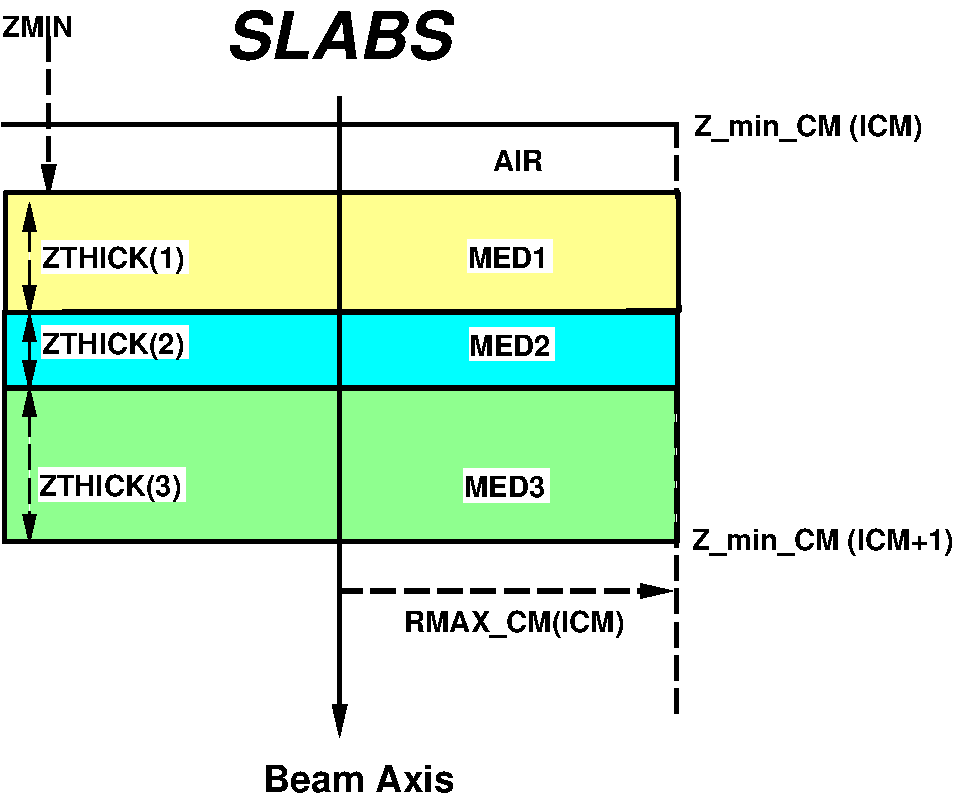
\includegraphics[height=9cm]{figures/slabsd}
\caption[SLABS CM geometry]
{Schematic of CM SLABS, which in the example
consists of three layers of different materials with thicknesses
{\tt ZTHICK(1)}, {\tt ZTHICK(2)}, and {\tt ZTHICK(3)},
respectively. The gap between the back of the
previous CM and the front face of this CM is automatically filled with air. The
outer boundary of this CM is a square of half-width {\tt RMAX\_CM}.}
\label{fig_SLABSD}
\end{center}
\end{figure}

\clearpage

The input format for SLABS, and an example of the input file are given as
follows.

\index{ESAVE!ESAVEIN}
\begin{small}
\index{SLABS!inputs}
\index{input file!for SLABS}
\input{./inputformats/SLABS.inp}
\end{small}





%\markright{CONS3R: ~~~~beamnrc\_um.tex~~~~printed \today~~ last edited 2004/11/19 20:21:18
%}
%\markboth{CONS3R Users Manual}{~~~~last edited 2004/11/19 20:21:18
%~~~~printed \today}

%\vspace*{1.5cm}
\subsubsection{CONS3R}
\renewcommand{\rightmark}{CONS3R CM}
\index{CONS3R}
\label{sCONS3R}

CONS3R is a stack of truncated cones coded as three regions.  It can be used
for any case if there is cylindrical symmetry and if there are only two
radial regions. Examples are slab, ring, stack rings, cone (primary
collimator),cone stack. The current version only allows convex shapes in
the Z direction, not concave shapes (\ie\ \verb+Z(I+1)+ is greater than
\verb+Z(i)+).  CONS3R is computationally more efficient than the other
conical CMs when there is more than one layer (\ie\ more than 3 node
points). This efficiency comes because there are only 2 Z boundaries for
particles to cross in CONS3R, no matter how many node points there are.

\begin{figure}[htbp]
\begin{center}
\htmlimage{scale=2.0}
\leavevmode
\mbox{}\hspace{0cm}
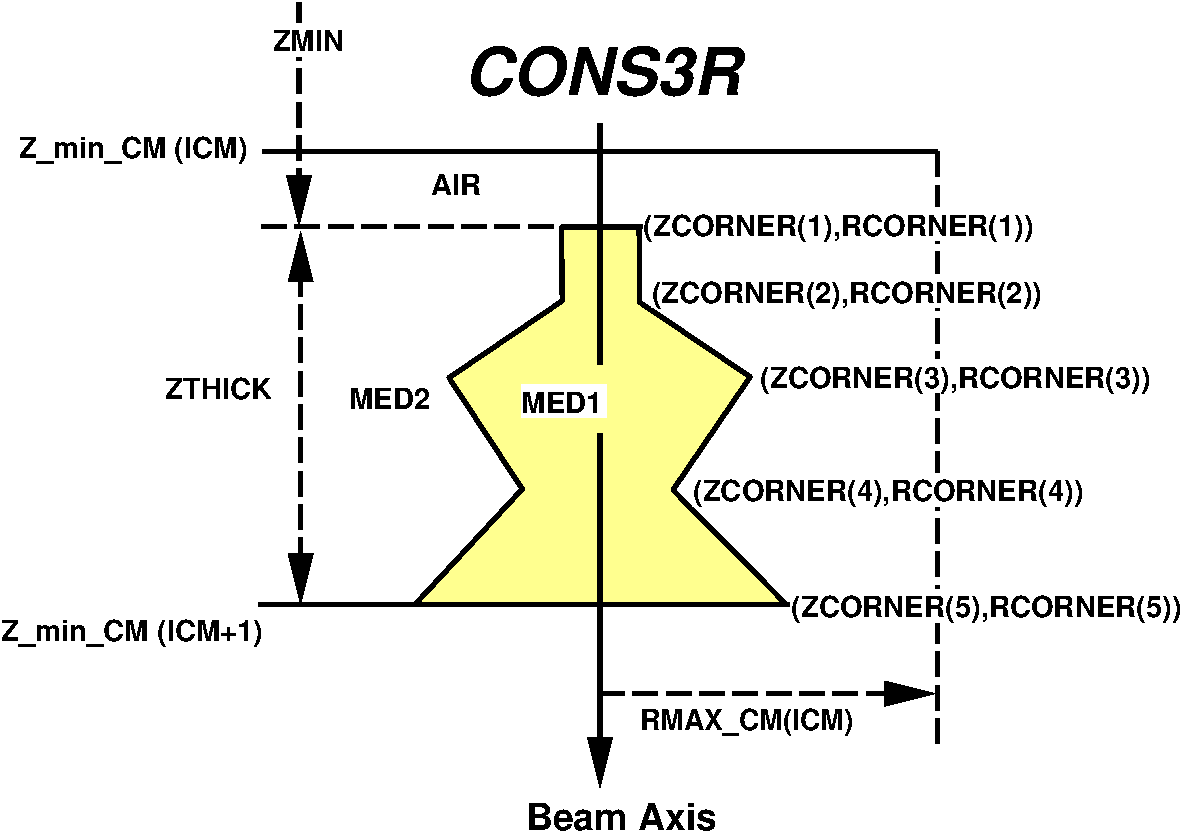
\includegraphics[height=9cm]{figures/cons3rd}
\caption[CONS3R CM geometry]
{Component module CONS3R defined by 5 node points, where RCORNER values can be
zero
and {\tt RCORNER(i+1)} can be smaller than {\tt RCORNER(i)}, but {\tt ZCORNER(i+1)} must be greater than or equal
to {\tt ZCORNER(i)}.  Z$_{\rm MIN}$ is the distance from the reference plane (Z = 0) to
the
front plane of the CM (excluding the air gap). The beam axis is an axis
of rotation and the outer boundary is a cylinder.}
\label{fig_CONS3RD}
\end{center}
\end{figure}

\clearpage

The input format for CONS3R, and an example of input file are given as follows.

\begin{small}
%\input{CONS3R.inputs}
\index{CONS3R!inputs}
\index{input file!for CON3R}
\input{./inputformats/CONS3R.inp}
\end{small}

\newpage

%\markright{CONESTAK: ~~~~beamnrc\_um.tex~~~~printed \today~~ last edited 2004/11/19 20:21:18
%}
%\markboth{CONESTAK Users Manual}{~~~~last edited 2004/11/19 20:21:18
%~~~~printed \today}


%\vspace*{1cm}
\subsubsection{CONESTAK}
\renewcommand{\rightmark}{CONESTAK CM}
\index{CONESTAK}

CONESTAK consists of a stack of coaxial truncated cones
surrounded by a cylindrical wall.
The vertices of the cones in each layer do not have to meet but the
radii
must not decrease as the depth increases.  This CM can model
scattering foils,  primary collimators and many other components.
CONESTAK has cylindrical symmetry.


\begin{figure}[htbp]
\begin{center}
\htmlimage{scale=2.0}
\leavevmode
\mbox{}\hspace{0cm}
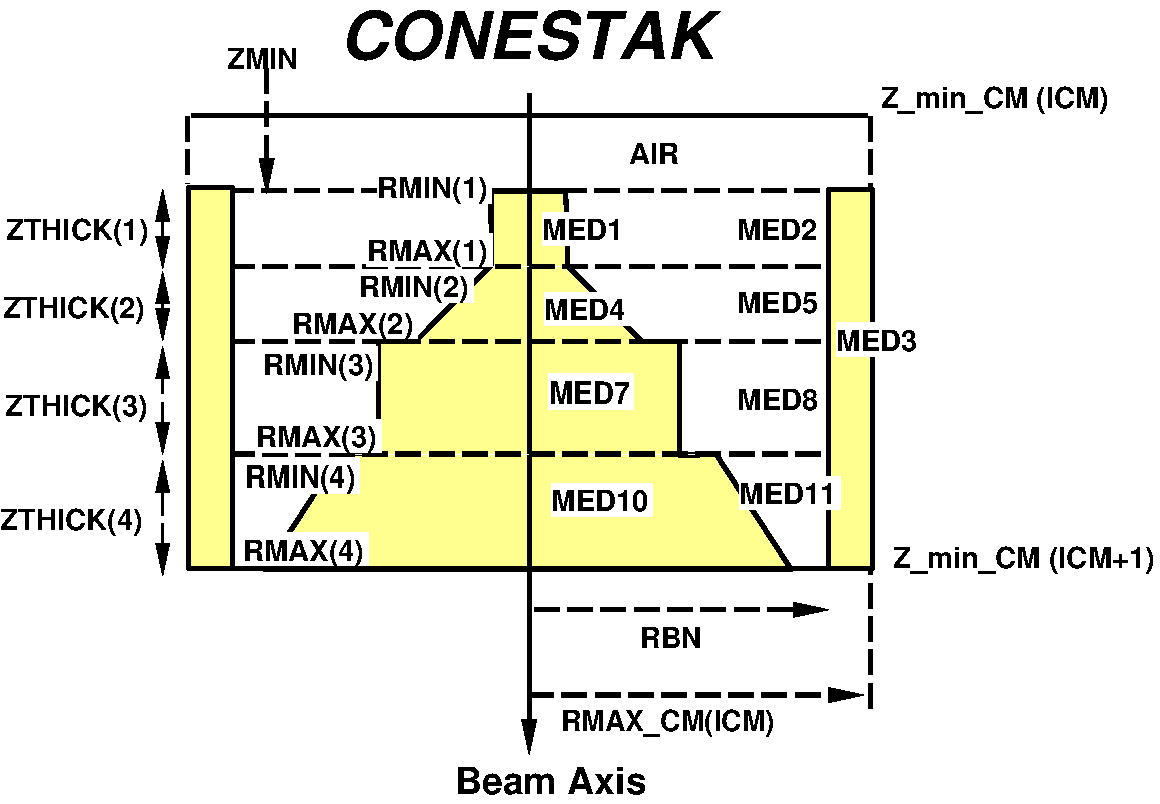
\includegraphics[height=11cm]{figures/conestakd}
\caption[CONESTAK CM geometry]
{CONESTAK with 5 layers ({\tt ISCM\_MAX}=5).  The outer wall has an inner
radius defined by {\tt RBN} and an outer radius equal to the outer boundary of
the CM ({\tt RMAX\_CM}).  Within each layer i, there is a cone with top and
bottom radii defined by {\tt RMIN(i)} and {\tt RMAX(i)} respectively.  Within each
layer, there are three regions: the inner cone, the
region between the cone and the outer wall (called the ``outer cone''), and the
outer
wall.  Regions 1,4,7,10,etc specify inner cones; regions 2,5,8,11,etc specify
outer cones; and regions 3,6,9,etc specify the outer wall.  If the user chooses
to have an outer wall (by setting {\tt RBN} $>$ 0) then the medium of region 3
, {\tt MED3}, is input first, even before {\tt MED1} and {\tt MED2}, and
{\tt MED3} is automatically applied to regions 6,9,etc, so that the outer
wall has the same composition in every layer.  If the user chooses not to
have an outer wall (by setting {\tt RBN} = 0), regions 3,6,9,etc shrink to
zero.
In specifying radii
of cones, the following restrictions apply: {\tt RMAX(i)} $\geq$ {\tt RMIN(i)}, and
{\tt RMIN(i+1)} $>$ {\tt RMAX(i)}.}
\label{fig_CONESTAKD}
\end{center}
\end{figure}

\clearpage

The input format for CONESTAK, and an example of input file are given as follows.

\begin{small}
\index{CONESTAK!inputs}
\input{./inputformats/CONESTAK.inp}
\index{input file!for CONESTAK}
\end{small}

\clearpage
%\markright{FLATFILT: ~~~~beamnrc\_um.tex~~~~printed \today~~ last edited 2004/11/19 20:21:18
%}
%\markboth{FLATFILT Users Manual}{~~~~last edited 2004/11/19 20:21:18
%~~~~printed \today}

\subsubsection{FLATFILT}
\renewcommand{\rightmark}{FLATFILT CM}
\index{FLATFILT}

FLATFILT consists of a stacked set of truncated coaxial cones with an arbitrary
number of cones on each level.  The material in the cones need not be the same.
Both the number of cones and the radii of cones in each layer can be specified
independently.  This CM can be used to model very complex beam flattening
filters for photon beam simulations, including those interior to a conical
collimator.
\begin{figure}[h]
\begin{center}
\leavevmode
\mbox{}\hspace{0cm}
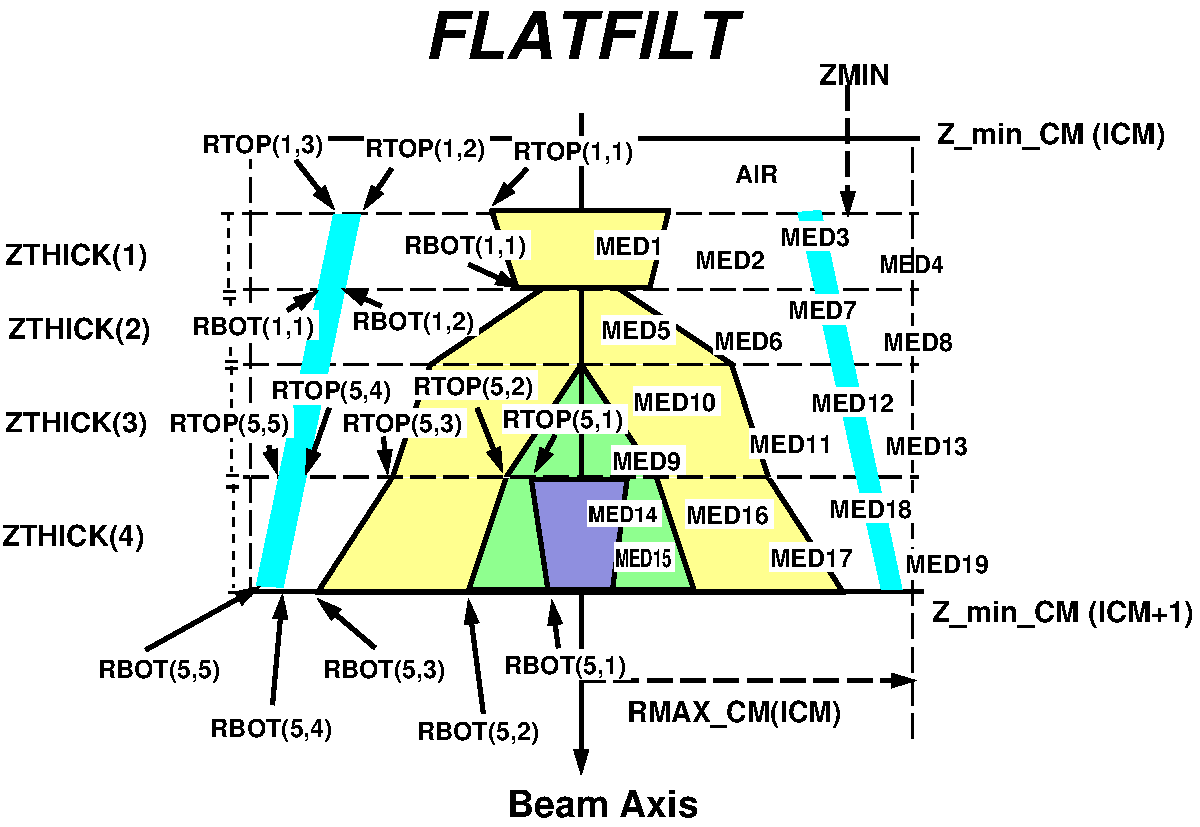
\includegraphics[width=16cm]{figures/flatfiltd}
\caption[FLATFILT CM geometry]
{FLATFILT with 4 layers ({\tt ISCM\_NO}=4).  Unlike CONESTAK, each layer can
have an arbitrary number of cones.  The number of cones in layer i is
specified by {\tt ISSCM\_NO(i)}.  Within a layer i, each cone j is specified by
its top and bottom radius, {\tt RTOP(i,j)} and {\tt RBOT(i,j)} respectively.  Within
a layer, cones cannot cross; so {\tt RTOP(i,j)} $<$ {\tt RTOP(i,j+1)} and
{\tt RBOT(i,j)} $<$ {\tt RBOT(i,j+1)}.  For each layer i, {\tt ISSCM\_NO(i)} + 1 media must be
specified.  {\tt ISSCM\_NO(i)} media are required for the cones, and the extra
medium is required for the region between the outermost cone and
{\tt RMAX\_CM}.  In the figure above, the 4 regions between outermost cones and
{\tt RMAX\_CM} are composed of {\tt MED4}, {\tt MED8}, {\tt MED13} and {\tt MED19}.}
\label{fig_FLATFILTD}
\end{center}
\end{figure}


\clearpage

\begin{small}
\index{FLATFILT!inputs}
\input{./inputformats/FLATFILT.inp}
\end{small}
\index{input file!for FLATFILT}

%\setlength{\textheight}{10.0in}
%\newpage
%\markright{CHAMBER: ~~~~beamnrc\_um.tex~~~~printed \today~~ last edited 2004/11/19 20:21:18
%}
%\markboth{CHAMBER Users Manual}{~~~~last edited 2004/11/19 20:21:18
%~~~~printed \today}

\subsubsection{CHAMBER}
\label{chamber_cm}
\renewcommand{\rightmark}{CHAMBER CM}
\index{CHAMBER}

CHAMBER models a parallel-plate ion chamber in a container with top and bottom
planes of arbitrary thickness and material. CHAMBER also
models a combination of scattering foils, cylindrical
collimators and an ion chamber, \etc. This CM is also useful for
central-axis
depth-dose calculations and for analysis of dose components due to
particles coming from different parts of an accelerator.
CHAMBER has cylindrical symmetry.

\begin{figure}[h]
\begin{center}
\leavevmode
\mbox{}\hspace{0cm}
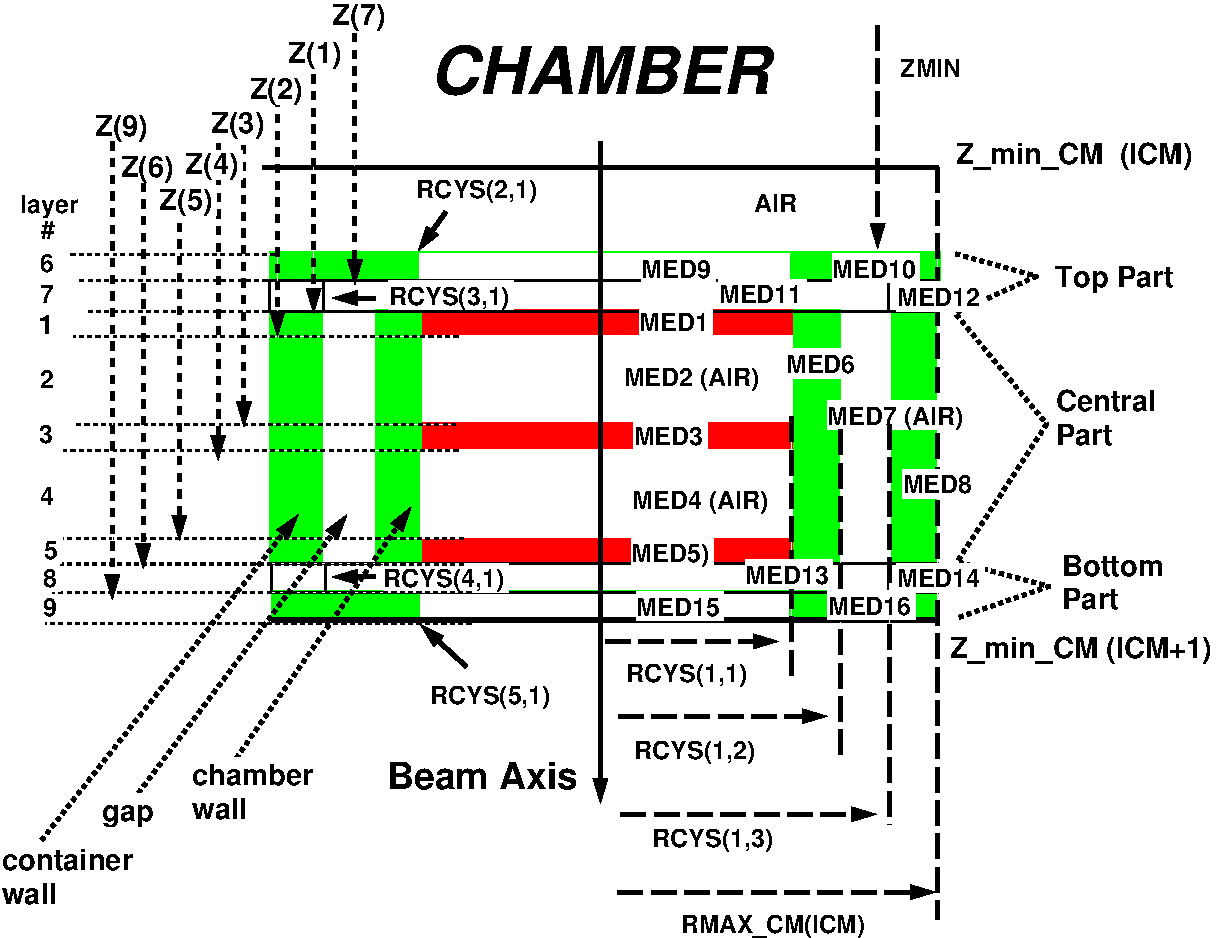
\includegraphics[height=9.0cm]{figures/chamberd}
\end{center}
\caption[CHAMBER CM geometry]
{CHAMBER component module for an ionization chamber or any symmetric
cylindrical-planar geometries. The CM shown consists of three parts: top,
central(chamber), and bottom.  The top and bottom parts each have 2
layers ({\tt N\_TOP = N\_BOT}=2),
and the chamber part has 5 layers ({\tt N\_CHM}=5).  In
general, the central part is required while the
top and bottom parts are not.  Each layer in both top and bottom parts
is divided into an inner cylinder and an outer annulus.  For a
layer i in the top part, the outer
radius of the cylinder (inner radius of the annulus) is given by
{\tt RCYS(i+1,1)}, and the outer radius of the annulus is {\tt RMAX\_CM}.
For a
layer j in the bottom part, the outer radius of the cylinder is
given by {\tt RCYS(j+N\_TOP+1,1)}, and outer radius of the annulus is
{\tt RMAX\_CM}.
Within the top or bottom part, layers can have different {\tt RCYS} and media;
however, input for the top or bottom part is simplified if all layers
within that
part have the same {\tt RCYS}, the same medium in the inner cylinders, and
the same medium in the outer annuli.  In the central part, all layers
have the same outer radius, {\tt RCYS(1,1)}, which also defines the inner
radius of the chamber wall.  The outer radius of the chamber wall is
given by {\tt RCYS(1,2)}, which, in turn, is the inner radius of the gap
between the chamber wall and the container wall.  The gap has outer
radius {\tt RCYS(1,3)}, which is also the inner radius of the container wall.
The container wall has outer radius {\tt RMAX\_CM}.}
\label{fig_CHAMBERD}
\end{figure}
\clearpage

%\vspace*{2cm}
\begin{figure}[htbp]
\begin{center}
\leavevmode
\mbox{}\hspace{0cm}
\begin{latexonly}
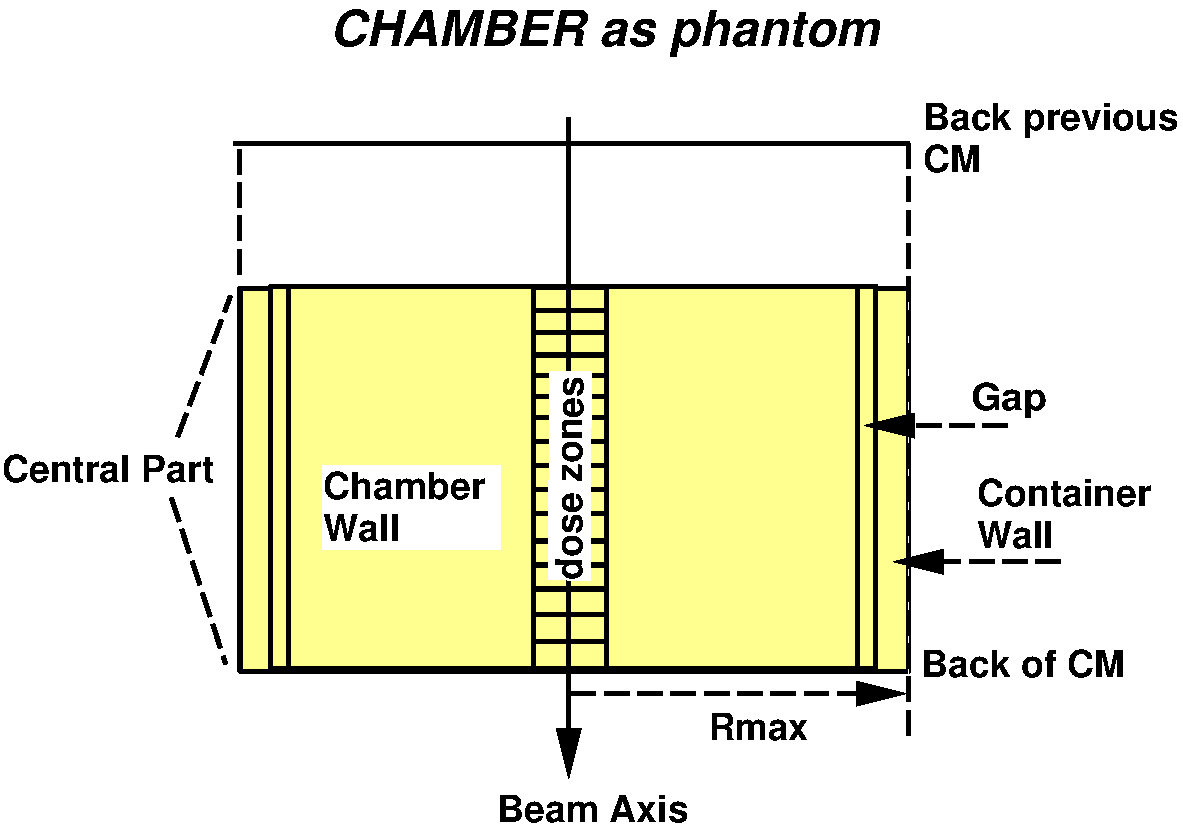
\includegraphics[height=9cm]{figures/chamberphant}
\end{latexonly}
\begin{htmlonly}
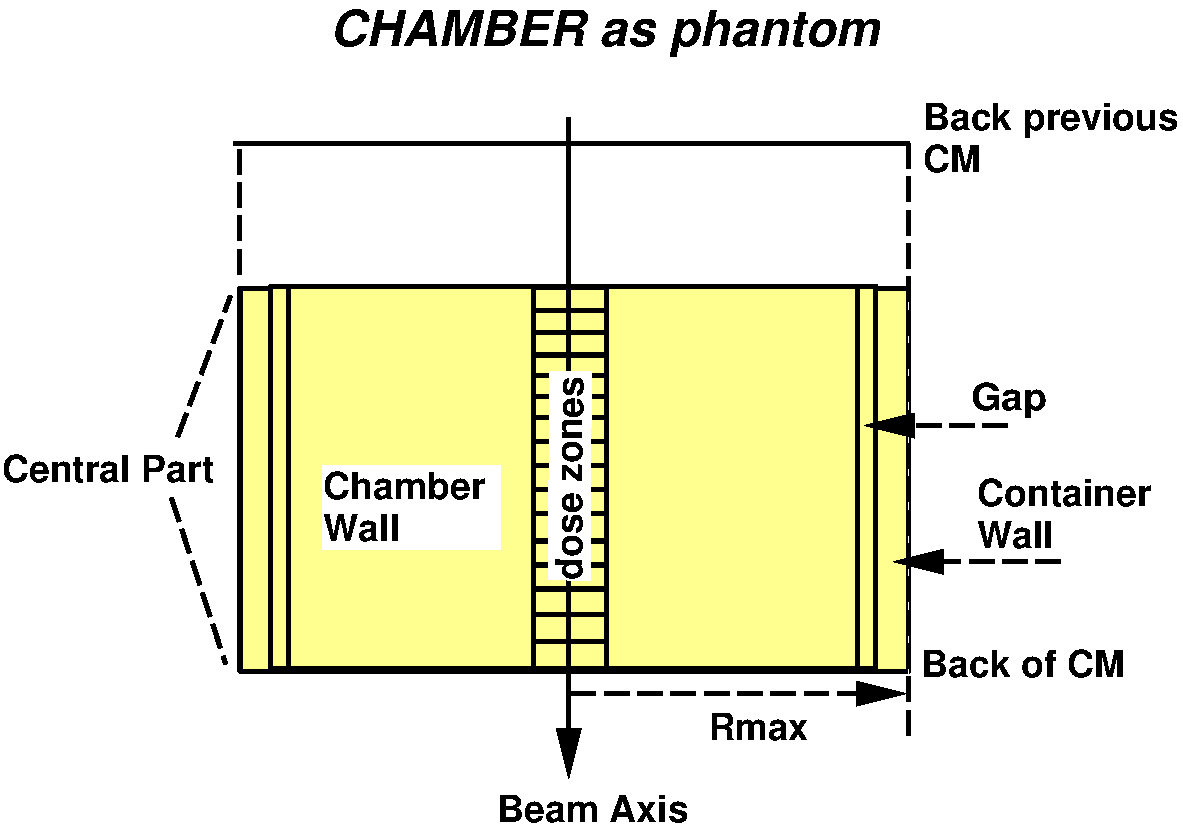
\includegraphics[height=8cm]{figures/chamberphant}
\end{htmlonly}
\end{center}
\caption[CHAMBER CM as a phantom]
{CHAMBER as a depth-dose phantom.  Only the central (chamber) part of
the CM is used.  The layers within this part become the depth-dose
zones, and, hence, all layers are composed of the same material (the
phantom material).  Depth resolution is determined by the number of
layers.  If all layers have the same thickness, then the input can
be made more efficient by inputting the number of layers on the same
line as the layer thickness, {\tt ZTHICK}.  Then you only have to
input {\tt ECUT}, {\tt PCUT}, {\tt DOSE\_ZONE} and {\tt MED} once for
all layers.  If {\tt DOSE\_ZONE} $>$0, the input value will be used
for the first layer and then {\tt DOSE\_ZONE} will be incremented by 1
automatically for each subsequent layer.
Alternatively, if there are N separate groups of layers, where the layers
in each group have equal thickness,
you can set {\tt N\_CHM\_\$CHAMBER} = -N.  For each of the N groups of
layers, you must specify the layer thickness and the number
of layers in the group.  Following this, you only have to specify
{\tt ECUT}, {\tt PCUT}, {\tt DOSE\_ZONE} and {\tt MED} once for all layers,
similar to the case where ALL layers are of equal thickness.
Note that all depth-dose zones have the same radius, determined by
{\tt RCYS}(1,1).
A small {\tt RCYS}(1,1) determines the depth-dose on the beam
axis, while a larger {\tt RCYS}(1,1) includes dose deposited further away from
the beam axis.  If the phantom extends beyond the radius of the dose
zones, then the chamber wall, gap, and container wall can be composed of
the same phantom material. This set-up can be very efficient for central
axis depth-dose calculations when used in conjunction with range
rejection because the large volume in the chamber wall leads to
effective range rejection. However, it has been observed for electron
beams that the lack of z boundaries in the wall region can lead to small
step size effects.  This effect can be minimised by decreasing
{\tt ESTEPE} (see section~\ref{ESTEPE}).}
\label{fig_CHAMBERPHANT}
\end{figure}

%\setlength{\textheight}{9.0in}

\clearpage

\index{input file!for CHAMBER}
\begin{small}
\index{CHAMBER!inputs}
\input{./inputformats/CHAMBER.inp}
\end{small}
\index{input file!for CHAMBER}

\newpage
%\setlength{\textheight}{10.0in}
%\markright{JAWS: ~~~~beamnrc\_um.tex~~~~printed \today~~ last edited 2004/11/19 20:21:18
%}

%\markboth{JAWS Users Manual}{~~~~last edited 2004/11/19 20:21:18
%~~~~printed \today}

\subsubsection{JAWS}
\label{jawssect}
\renewcommand{\rightmark}{JAWS CM}
\index{JAWS}

JAWS is used for a set of paired bars, which can be bars in the collimator or
applicator. The bars are of arbitrary thickness and material, and X or Y
orientation.  The outer boundary of JAWS has square symmetry but the jaws
themselves can be very asymmetric. The input for JAWS can be tedious
but the GUI has a feature which will automatically set the X and Y values
to give an arbitrary on-axis rectangular photon beam field size at a
given SSD based on tracing back to an arbitrary focus located on the
central axis.
\index{GUI}

\begin{figure}[htbp]
\label{fig_JAWSD}
\begin{center}
\leavevmode
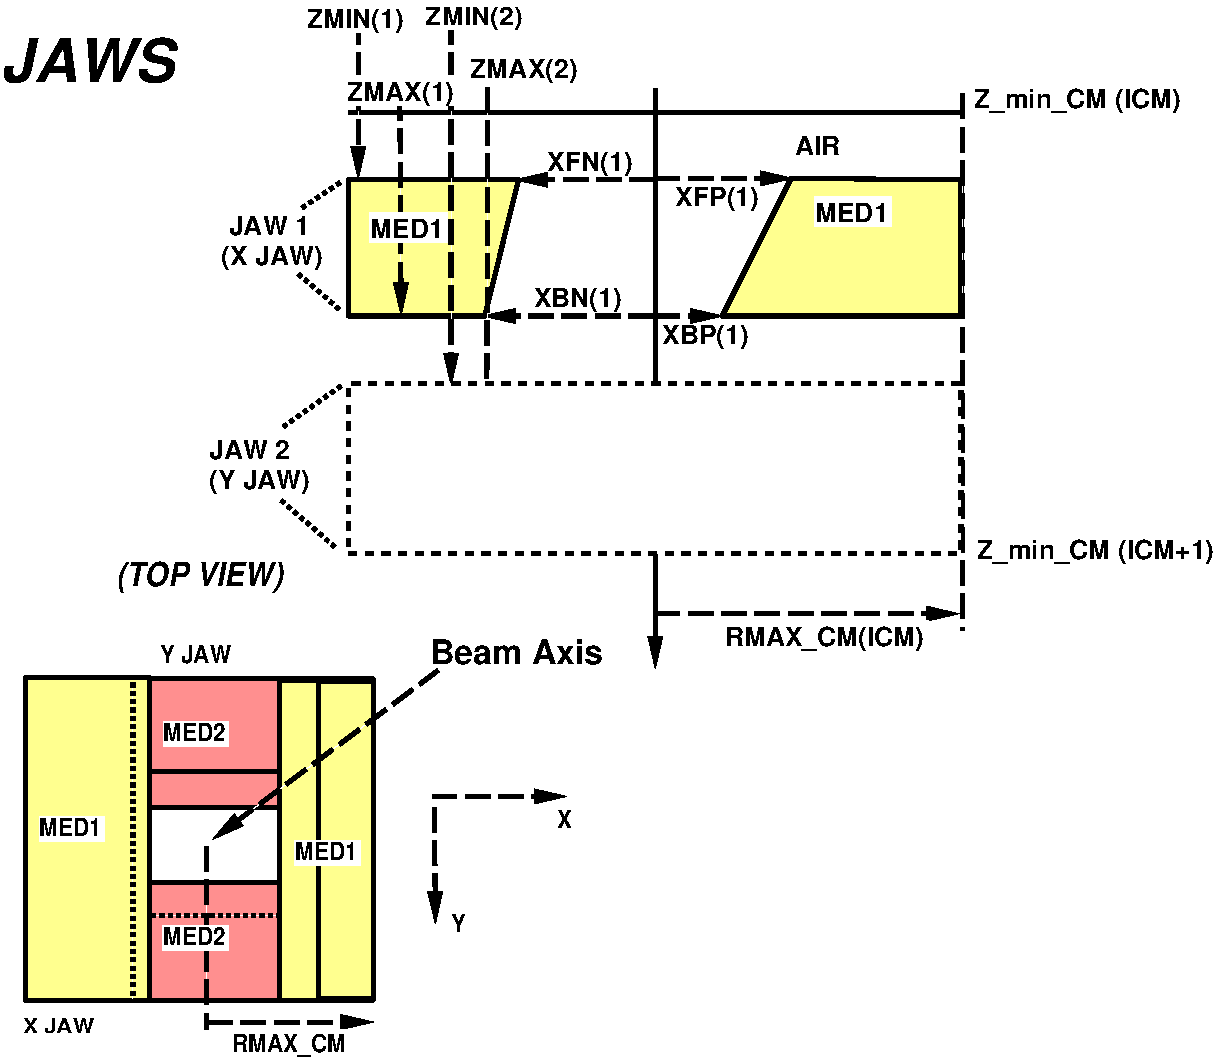
\includegraphics[height=12cm]{figures/jaws-both}
\end{center}
\caption[JAWS CM geometry]
{JAWS component module with paired X
and Y jaws ({\tt ISCM\_MAX=2}).  The cutaway view cuts right through the
opening in the Y jaws, hence the representation of the Y jaws as a dashed
rectangle.  For a set of jaws i, the front opening of the jaws
is specified by {\tt XFP(i)} and {\tt XFN(i)}.
The back opening is specified by
{\tt XBP(i)} and {\tt XBN(i)}.
These coordinates are not shown for the Y jaws,
however they are evident in the top view.  The inside jaw surfaces are 2 planes,
one connecting
{\tt XFP(i)} to {\tt XBP(i)} and the other connecting {\tt XFN(i)}
to {\tt XBN(i)}  X jaws and
openings between X jaws extend
to $\pm$ {\tt RMAX\_CM} in the Y-direction; Y jaws and openings extend
to $\pm$ {\tt RMAX\_CM} in the X
direction.  There must be a gap of at least 0.01 cm between the first
set of jaws and the top of the CM (\ie\ {\tt ZMIN(1)-ZMIN\_CM} $\geq$ 0.01) and
between sets of jaws (\ie\ {\tt ZMIN(i)-ZMAX(i-1)} $\geq$ 0.01).
Materials in each layer can be different but opposite jaws must be the
same material.}
\end{figure}

%\setlength{\textheight}{9.0in}
\clearpage

The input format for JAWS, and an example of input file are
given as follows.


\begin{small}
\index{JAWS!inputs}
\input{./inputformats/JAWS.inp}
\end{small}
\index{input file!for JAWS}

%\setlength{\textheight}{10.0in}
%\markright{APPLICAT: ~~~~beamnrc\_um.tex~~~~printed \today~~ last edited 2004/11/19 20:21:18
%\clearpage
%}
%\markboth{APPLICAT Users Manual}{~~~~last edited 2004/11/19 20:21:18
%~~~~printed \today}

\clearpage
\vspace*{-1cm}
\subsubsection{DYNJAWS}
\label{dynjawssect}
\renewcommand{\rightmark}{DYNJAWS CM}
\index{DYNJAWS}

DYNJAWS is a version of JAWS (see Section~\ref{jawssect} above) which allows the
user to specify changing jaw settings (Z positions and opening coordinates)
over the course of a simulation.  There are two dynamic modes: ``step-and-shoot"
({\tt MODE\_\$DYNJAWS}=2) and ``dynamic"
({\tt MODE\_\$DYNJAWS}=1).  If being run in one of these modes, then the user must
specify the jaw settings in a separate file.  The format of this file is:
\begin{verbatim}
TITLE
NFIELD
FOR I=1,NFIELD[
INDEX(I)
FOR J=1,ISCM_MAX[
ZMIN(J,I),ZMAX(J,I),XFP(J,I),XBP(J,I),XFN(J,I),XBN(J,I)
]
]
\end{verbatim}
where:
\begin{description}
\item[{\tt TITLE}] is a title line for the file.
\item[{\tt NFIELD}] = the number of ``sets" of jaw settings, or fields.
\item[{\tt INDEX(I)}] = the index of field I, where 0$\leq${\tt INDEX(I)}$\leq$1 and
 {\tt INDEX(I)}$>${\tt INDEX(I-1)}.
\item[{\tt ISCM\_MAX}] = the number of jaws.
\item[{\tt ZMIN(J,I)}] = the Z position of the front of jaw J for field I.
\item[{\tt ZMAX(J,I)}] = the Z position of the back of jaw J for field I.
\item[{\tt XFP(J,I)}] = the front X or Y coordinate (depending on
jaw orientation) of the positive bar of jaw J for field I.
\item[{\tt XBP(J,I)}] = the back X or Y coordinate of the positive bar of jaw J
for field I.
\item[{\tt XFN(J,I)}] = the front X or Y coordinate of the negative bar of jaw J for field I.
\item[{\tt XBN(J,I)}] = the back X or Y coordinate of the negative bar of jaw J
for field I.
\end{description}

The parameter, {\tt INDEX(I)}, is used to determine which field is used
for a given primary history simulated.  At the beginning of each primary
history a random number, {\tt RND}, on [0,1] is chosen and compared to
the {\tt INDEX(I)}.  The field no. used is the lowest value of {\tt I} for
which {\tt RND}$\leq${\tt INDEX(I)}.  If the user has selected ``step-and-shoot" mode,
then the jaw settings for field {\tt I} are simply used.  If the user has
selected ``dynamic'' mode, then the jaw settings are a linear interpolation between
field {\tt I-1} and {\tt I} based on the value of {\tt RND}.  For example, the
Z position of the front of jaw J, {\tt ZMIN(J)}, would be given by:
\begin{equation}
{\tt
ZMIN\left(J\right)=ZMIN\left(J,I-1\right)+\frac{\left[ZMIN\left(J,I\right)-ZMIN\left(J,I-1\right)\right]}
{\left[INDEX\left(I\right)-INDEX\left(I-1\right)\right]}\times\left[RND-INDEX\left(I-1\right)\right]
}
\end{equation}
In this way, the ``dynamic'' mode simulates jaw motion while the beam is
on.

Note that the user can also select ``static'' mode, in which the inputs are identical
to JAWS and jaw settings are fixed.

An example file containing the jaw settings for 3 fields for a single jaw are contained in
the file {\tt \$OMEGA\_HOME/beamnrc/CMs/sample\_dynjaws.sequence}.

The input format for DYNJAWS, and an example of an input are
given as follows.

\begin{small}
\index{DYNJAWS!inputs}
\input{./inputformats/DYNJAWS.inp}
\end{small}
\index{input file!for DYNJAWS}

\clearpage
\vspace*{-1cm}
\subsubsection{SYNCJAWS}
\renewcommand{\rightmark}{SYNCJAWS CM}
\index{SYNCJAWS}
SYNCJAWS is a version of DYNJAWS (See Section~\ref{dynjawssect} above) in which the
``dynamic'' or ``step-and-shoot'' jaw settings (opening coordinates and Z-positions) specified
in a file are synchronized with the settings of any other synchronized CMs (SYNCVMLC, SYNCMLCE,
SYNCHDDMLC) in the accelerator and with the motion of source 20 (synchronized phase space) or
source 21 (synchronized BEAM treatment head simulation) in DOSXYZnrc\cite{Wa05}.  SYNCJAWS was
contributed by Julio Lobo and Tony Popescu\cite{LP10}.

\index{muIndex(I)}
Inputs to SYNCJAWS are identical to those for DYNJAWS.  The DYNJAWS input, {\tt INDEX(I)}, used in dynamic
and step-and-shoot modes to determine the cumulative probability of field {\tt I} being used for
an incident history, is now interpreted as {\tt muIndex(I)}, the fraction of total monitor units
delivered up to and including field {\tt I}.

\index{MU\_RND}
Similar to DYNJAWS, at the beginning of each primary history, a random number, {\tt MU\_RND}$\in[$0,1$]$, is
compared to the {\tt muIndex(I)} and used to determine the field number and jaw settings used.  In dynamic mode,
the equation for calculating jaw settings is the same as Equation (6) above, with {\tt muIndex} replacing
{\tt INDEX} and {\tt MU\_RND} replacing {\tt RND}.

\index{DOSXYZnrc!sources 20 and 21}
The only difference between
DYNJAWS and SYNCJAWS is that the value of {\tt MU\_RND} used by SYNCJAWS for each primary history is the same as
that used by any other synchronized CMs in the accelerator.  {\tt MU\_RND} is generated by the first (most upstream) synchronized
CM (which could be SYNCJAWS) and is then passed on to any downstream synchronized CMs.
Thus, the dynamic motion of the jaws can be coordinated (synchronized) with the dynamic motion of all other synchronized CMs
in the the accelerator.  Moreover, if an accelerator with synchronized CMs has been compiled as a shared library for use
in DOSXYZnrc source 20
(synchronized phase space source) or source 21 (synchronized BEAM treatment head simulation), then {\tt MU\_RND} is passed from the
accelerator simulation to DOSXYZnrc.  This allows the dynamic motion of the source plane in DOSXYZnrc sources 20 and 21 to be synchronized with
the settings of the CMs in the accelerator.
Note that it is up to the user to set up the synchronization between CMs within the accelerator, using the files defining jaw
settings and, for MLC's, leaf opening coordinates for each field, and between the CM parameters and the motion of
DOSXYZnrc source 20 or 21.
See the DOSXYZnrc Users Manual\cite{Wa05} for more information on sources 20 and 21.

An example of a file specifying dynamic jaw settings for SYNCJAWS
is included with the distribution.  This file is {\tt \$OMEGA\_HOME/beamnrc/CMs/sample\_syncjaws.sequence}.

\clearpage
\vspace*{-1cm}
\subsubsection{APPLICAT}
\renewcommand{\rightmark}{APPLICAT CM}
\index{APPLICAT}

APPLICAT is used for a set of rectangular scrapers. Each scraper is defined by
the outer region of two concentric rectangles, the inner region being air.  The
scrapers are of arbitrary thickness, width in both X and Y directions, and
position relative to the
reference plane ($Z = 0$). The scrapers can be  of different  materials.
This CM may be used for modelling the square applicator found in electron
beams although it does
not allow for a bevelled edge.  The outer boundary of APPLICAT is a square
centered on the beam axis.

\begin{figure}[htp]
\begin{center}
\htmlimage{scale=2.0}
\leavevmode
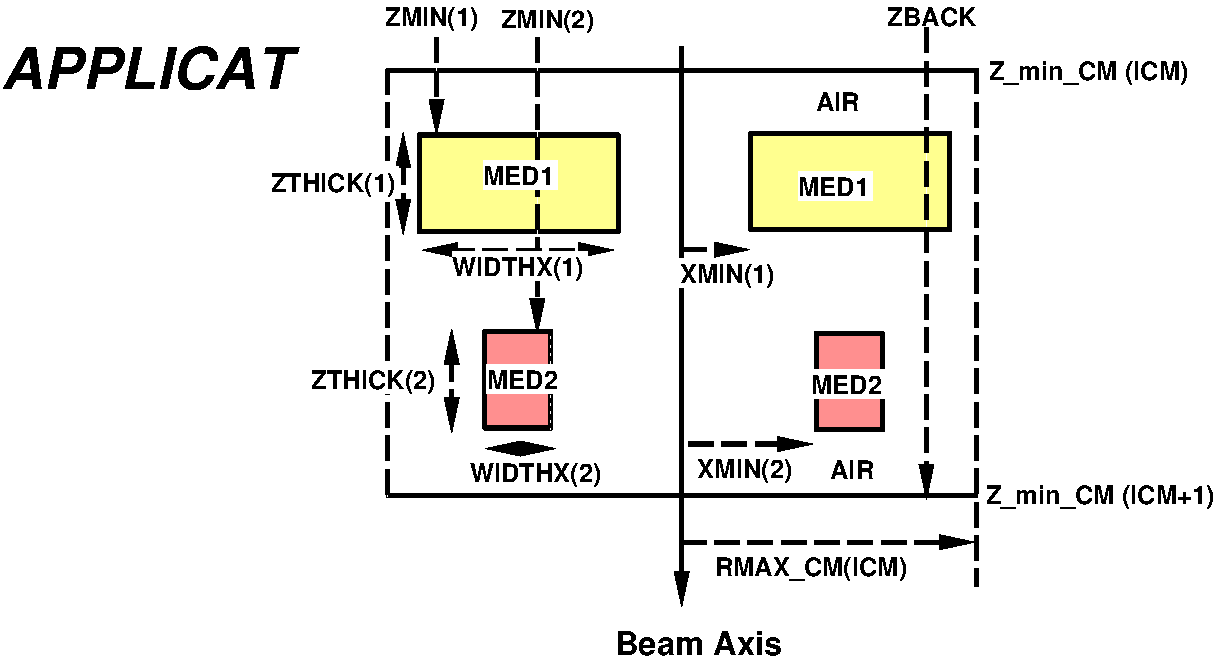
\includegraphics[height=9.25cm]{figures/applicatd}
\end{center}
\vspace{-1.6cm}
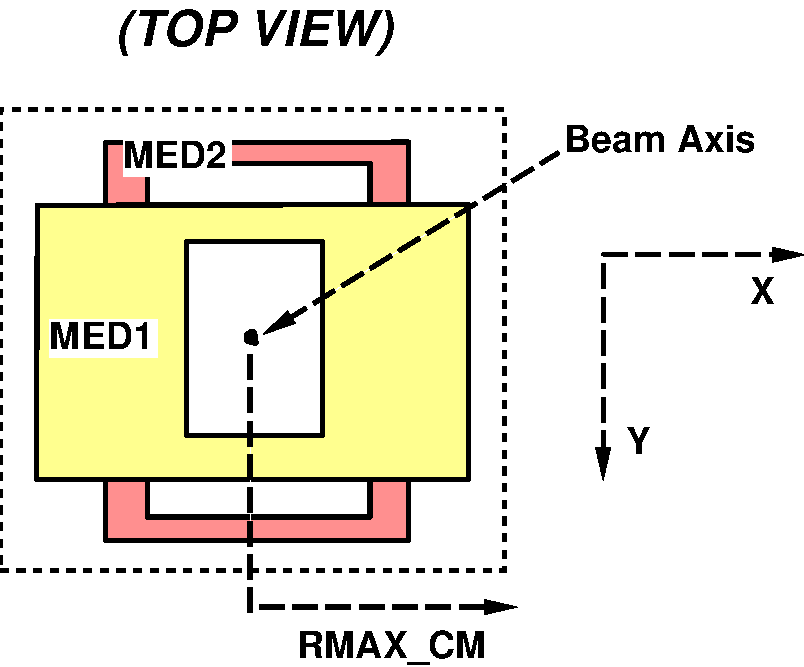
\includegraphics[height=6cm]{figures/applicattop}
\caption[APPLICAT CM geometry]
{An APPLICAT with 2 scrapers ({\tt N}=2).  Each scraper i has a rectangular opening in
the centre with half-width in the X-direction {\tt XMIN(i)} and half-width in
the Y-direction {\tt YMIN(i)}
.  The width of scraper i in the
X-direction is given by
{\tt WIDTHX(i)} and in the Y-direction by {\tt WIDTHY(i)}.  The cross section does
not show the Y dimensions of the scrapers, however the Y dimensions are
evident in the top view.  The minimum space
between two scraper is 0.01
cm of air.  There is also a minimum 0.01 cm air gap at the front (ie
between {\tt Z\_min\_CM(1)}
 and {\tt ZMIN(1))} and back (\ie\ between {\tt ZBACK} and the back
of the last scraper) of
the CM.}
\index{ZBACK}\index{Z\_min\_CM}
\label{fig_APPLICATD}
\end{figure}

%\setlength{\textheight}{9.0in}
\clearpage

The input format for APPLICAT, and an example of input file are given as follows.

\begin{small}
\index{APPLICAT!inputs}
\input{./inputformats/APPLICAT.inp}
\end{small}
\index{input file!for APPLICAT}

\clearpage
\vspace*{-1cm}
\subsubsection{CIRCAPP}
\renewcommand{\rightmark}{CIRCAPP CM}
\index{CIRCAPP}

CIRCAPP is similar to APPLICAT, however, it is used to model scrapers that have
circular openings.  The scrapers retain their rectangular outer edges, but
the opening is now defined as a circle concentric with the rectangle
defining the outer edges.  Similar to APPLICAT, CIRCAPP does not allow
bevelled edges. The outer boundary of CIRCAPP is a square centered on the beam axis.

\begin{figure}[htp]
\begin{center}
\leavevmode
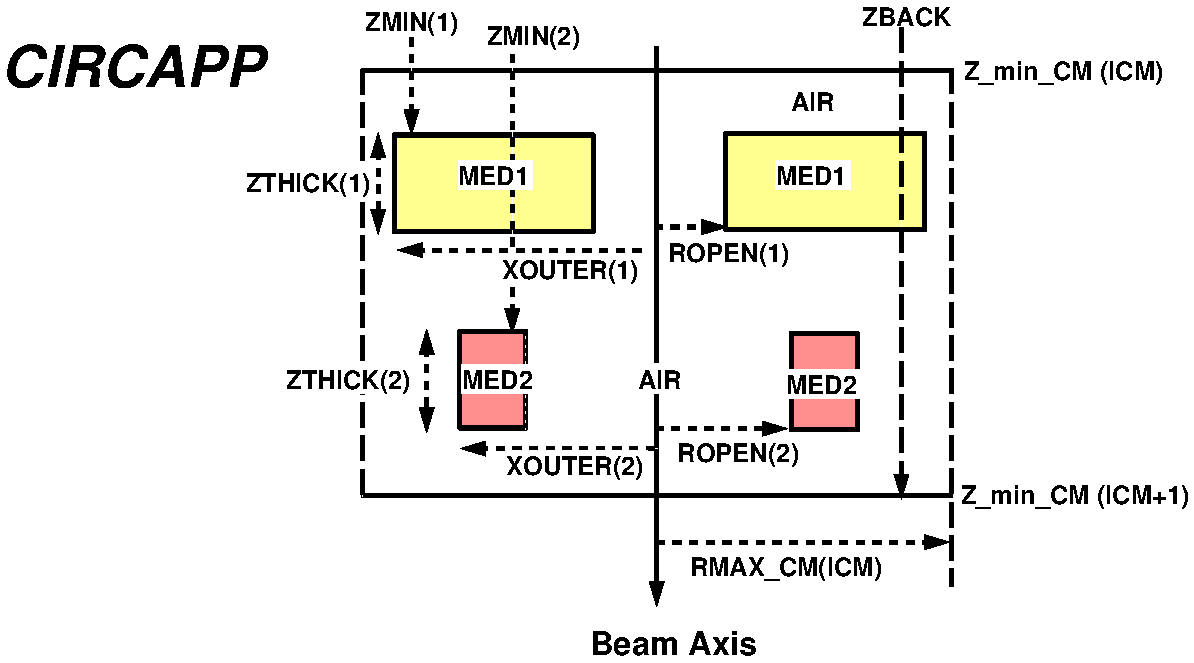
\includegraphics[height=9.25cm]{figures/circappd}
\end{center}
\vspace{-1.6cm}
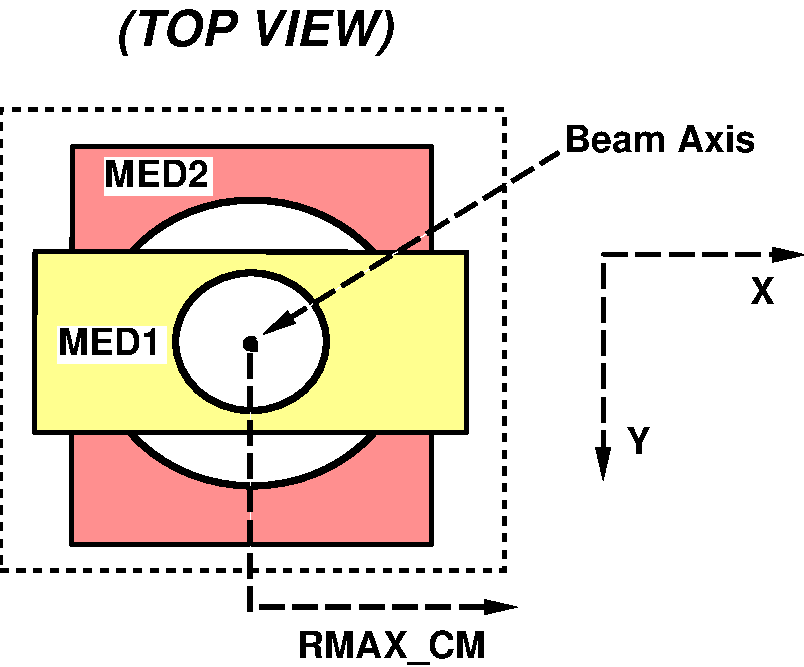
\includegraphics[height=6cm]{figures/circapptop}
\caption[CIRCAPP CM geometry]
{A CIRCAPP with 2 scrapers ({\tt N}=2).  Each scraper i has half-widths in the
X- and Y-directions given by {\tt XOUTER(i)} and {\tt YOUTER(i)} and a
circular opening in the centre with radius {\tt ROPEN(i)}.
The Y dimensions are not shown in the cross section, however, they
are apparent in the top view.  As in APPLICAT, there are minimum air gaps
of 0.01~cm between scrapers, between {\tt Z\_min\_CM(1)} and the first scraper
and between {\tt ZBACK} and the last scraper.}
\index{ZBACK}\index{Z\_min\_CM}
\label{fig_CIRCAPPD}
\end{figure}

\clearpage

The input format for CIRCAPP, and an example of input file are given as follows.

\begin{small}
\index{CIRCAPP!inputs}
\input{./inputformats/CIRCAPP.inp}
\end{small}
\index{input file!for CIRCAPP}

%\setlength{\textheight}{10.0in}
%\clearpage

%\markboth{PYRAMIDS Users Manual}{~~~~last edited 2004/11/19 20:21:18
%~~~~printed \today}

\subsubsection{PYRAMIDS}
\renewcommand{\rightmark}{PYRAMIDS CM}
\index{PYRAMIDS}
The PYRAMIDS CM is used to model pyramid-shaped structures comprising
one or more layers in the path of
the beam.  Each layer has three distinct regions: the central region
(the pyramid), the
surrounding region and the outer region (beyond the outer edges of the layer).
The central and outer regions default to air but can also be filled
with a user-specified medium (assumed the same for the central and outer
regions within a layer).
PYRAMIDS is useful for modelling rectangular collimators and beam blocks.
This CM has a square outer boundary centered on
the beam axis.

\newpage

\begin{figure}[tp]
\htmlimage{scale=1.5}
\leavevmode
\hfill
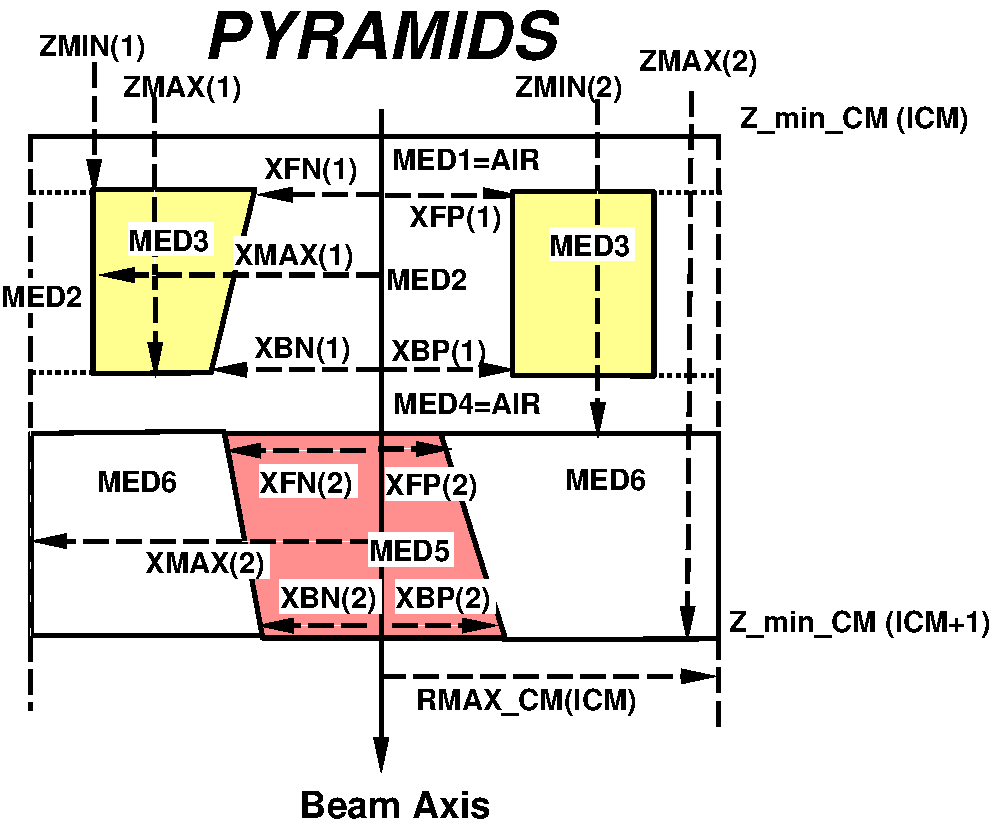
\includegraphics[height=10.5cm]{figures/pyramidsd}
\vspace{0.1cm}
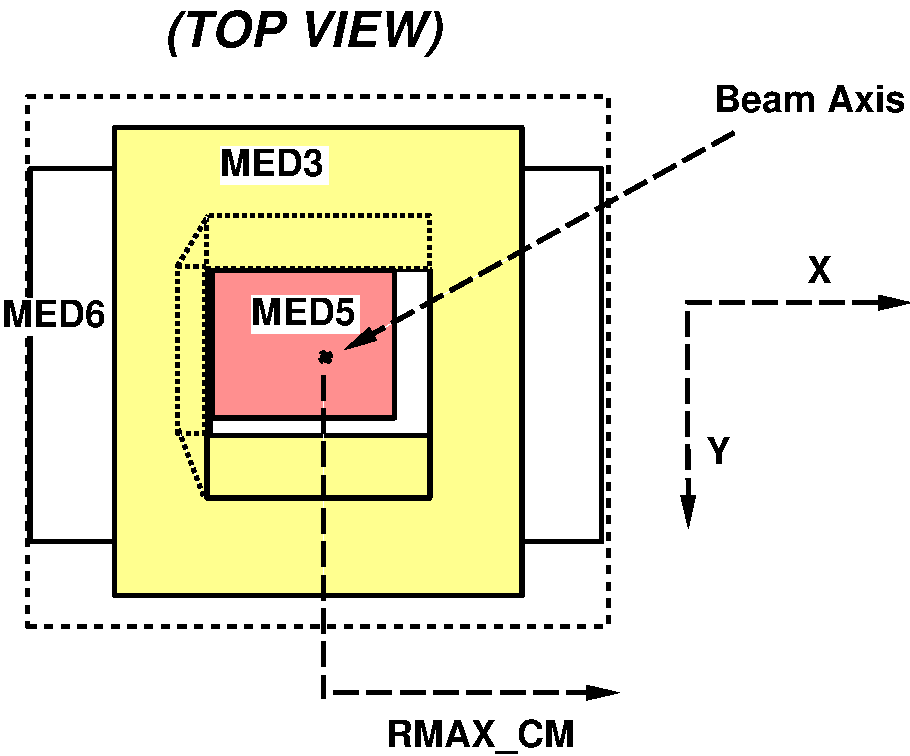
\includegraphics[height=6.0cm]{figures/pyramidstop}
\caption[PYRAMIDS CM geometry]
{A PYRAMIDS component module with 2 layers ({\tt ISCM\_MAX}=2).  Within a
layer i, the front of the central region is specified by
{\tt XFP(i)}, {\tt XFN(i)}, {\tt YFP(i)}, {\tt YFN(i)}, and the back
is defined by {\tt XBP(i)}, {\tt XBN(i)}, {\tt YBP(i)},
{\tt YBN(i)}.
The central region's inner faces are the planes connecting rectangle
defining the front of the region with that defining the back of the region.
The X and Y outer edges of
layer i are defined by {\tt XMAX(i)} and {\tt YMAX(i)} respectively.
The figure does
not show the Y dimensions (\ie\ {\tt YFN(i)}, {\tt YFP(i)}, {\tt YMAX(i)}, \etc.),
however the Y
dimensions are evident in the top view.  Layers must be separated by at
least 0.01cm ({\tt ZMIN(i+1)}-{\tt ZMAX(i)} $\geq$ 0.01cm).  By setting
{\tt IFILL=1},
the user can set the medium filling the central and outer regions
in each layer ({\tt MED2} and {\tt MED5}).  The gaps
between layers are assumed to be filled with air.}
\label{fig_PYRAMIDSD}
\end{figure}

%\setlength{\textheight}{9.0in}

\clearpage
The input format for PYRAMIDS and an example input are given below.
\begin{small}
\index{PYRAMIDS!inputs}
\input{./inputformats/PYRAMIDS.inp}
\end{small}
\index{input file!for PYRAMIDS}

%\setlength{\textheight}{10.1in}

%\clearpage

%\markboth{BLOCK Users Manual}{~~~~last edited 2004/11/19 20:21:18
%~~~~printed \today}

\subsubsection{BLOCK}
\renewcommand{\rightmark}{BLOCK CM}
\index{BLOCK}
The BLOCK CM is used to model a treatment block having non-rectangular
and/or multiple openings.  The user specifies openings in the block
material using up to 20 ``subregions''.  For each subregion the user
specifies the X-Y coordinates of its vertices at the top surface of the
block material (either clockwise or counter-clockwise around the
perimeter).  The inner planes of all subregions are angled with respect to
the beam (Z) axis towards a single user-specified ``focus point'' on the
beam axis.  Note that no subregion can have an inner
angle $>$~180 degrees.
Openings can consist of a single subregion or may require
several adjoining subregions in order to avoid the restriction on the inner
angles.
The user also specifies the X and Y coordinates
of the 4 outer edges of the block material, so the material need not
extend to the square outer boundary of this CM.  Due to its generality,
BLOCK may require up to 2 times the CPU time of PYRAMIDS to simulate
simple rectangular geometries; thus, PYRAMIDS is recommended when there is
a single rectangular opening.

The current version of BLOCK has been significantly changed from
BLOCK in BEAM99 (see {\tt CHANGES\_from\_BEAM99.for.BEAM00}).  This
is because John Antolak of the M.D. Anderson Cancer Center found and
corrected some serious errors in this CM.

\newpage
\begin{figure}[tp]
\begin{center}
\leavevmode
\begin{latexonly}
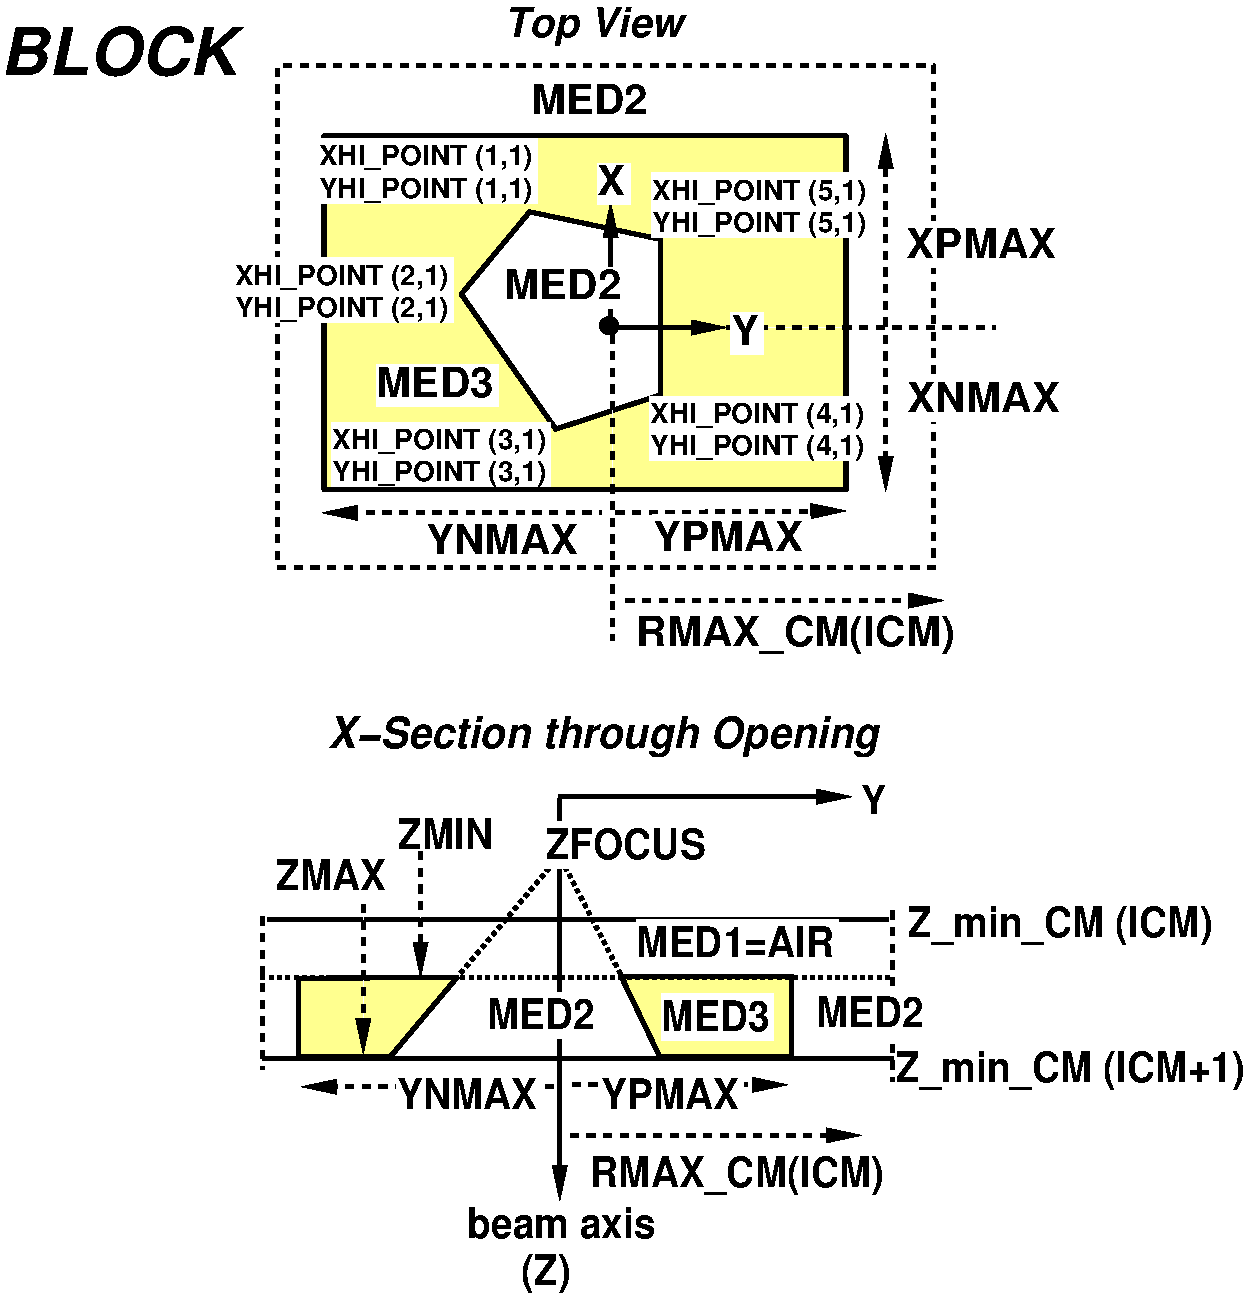
\includegraphics[height=15cm]{figures/blockd}
\end{latexonly}
\begin{htmlonly}
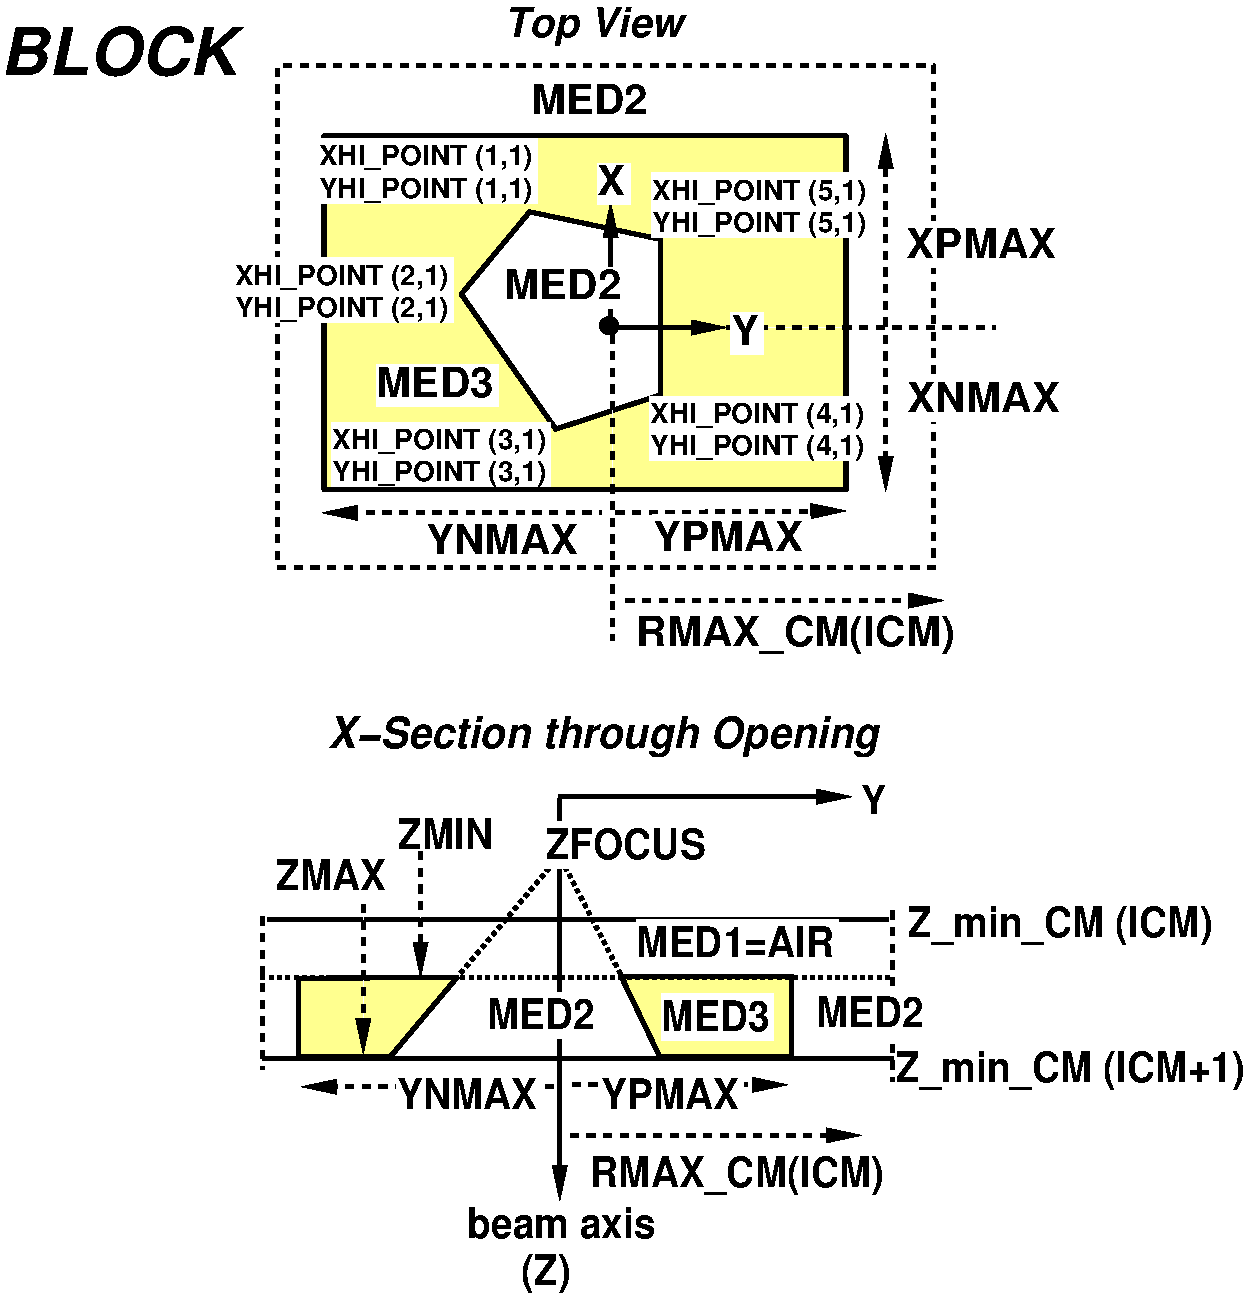
\includegraphics[height=14cm]{figures/blockd}
\end{htmlonly}
\end{center}
\vspace{1cm}
\caption[BLOCK CM geometry]
{A BLOCK component module with a single opening composed of 1
subregion ({\tt ISUB\_MAX}=1).  As shown in the top view, the subregion
has 5 vertices ({\tt NSUB(1)}=5).  The X-Y coordinates of the vertices
at the top surface of the block material are specified counter-clockwise
around the perimeter of the subregion, beginning with
({\tt XHI\_POINT(1,1)},{\tt YHI\_POINT(1,1)}).  Also shown in the top
view are the coordinates defining the outer boundary of the block,
{\tt XPMAX}, {\tt YPMAX}, {\tt XNMAX} and {\tt YNMAX}.
The cross-section through
the opening shows that the planes defining the inner surfaces of the
subregion/opening are all angled with respect to the Z-axis towards the
single focus point on the Z-axis.  Note that there must be an air gap
between {\tt ZMIN} and {\tt Z\_min\_CM(ICM)} of $\geq$ 0.01 cm.  Note that
the user specifies MED2, the material filling the opening(s) and the region
beyond the block edges.
The top gap is assumed to be air.  More complicated
opening shapes may require several adjoining subregions.}
\label{fig_BLOCKD}
\end{figure}

%\setlength{\textheight}{9.0in}

\clearpage
The input format for BLOCK and an example input are given below.
\begin{small}
\index{BLOCK!inputs}
\input{./inputformats/BLOCK.inp}
\end{small}
\index{input file!for BLOCK}



%\setlength{\textheight}{10.0in}

%\clearpage

%\markboth{MLC Users Manual}{~~~~last edited 2004/11/19 20:21:18
%~~~~printed \today}

\subsubsection{MLC}
\renewcommand{\rightmark}{MLC CM}
\index{MLC}
\index{multi-leaf collimator!MLC}
The MLC CM is used to model a double-focusing multi-leaf collimator with
flat faces.
The collimator has a single layer with a user-specified number of leaves
all opening in either the X or Y direction.  The collimator opening is
specified by the coordinates of the individual leaf openings at the top of the
collimator, the thickness of the leaves in the Z direction, and two
Z ''foci'' that determine the angles of the leaf side and end
surfaces.
The outer boundary of the MLC CM is a square centred on
the beam axis.  Currently, the collimator body extends to this outer boundary.

\newpage
\begin{figure}[tp]
\begin{center}
\leavevmode
\begin{latexonly}
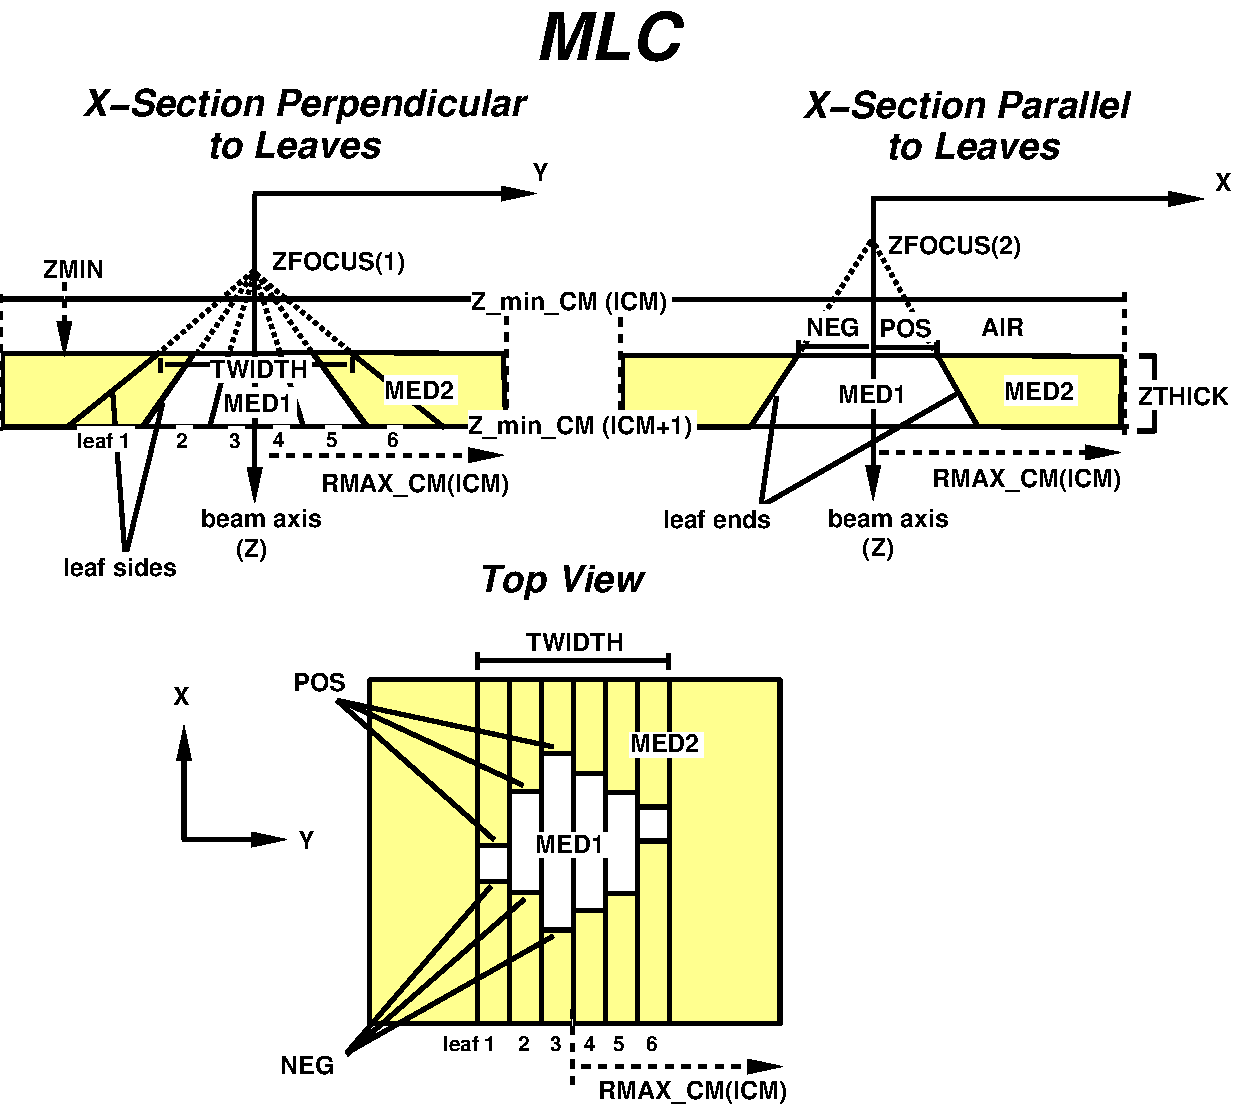
\includegraphics[height=13cm]{figures/mlcd}
\end{latexonly}
\begin{htmlonly}
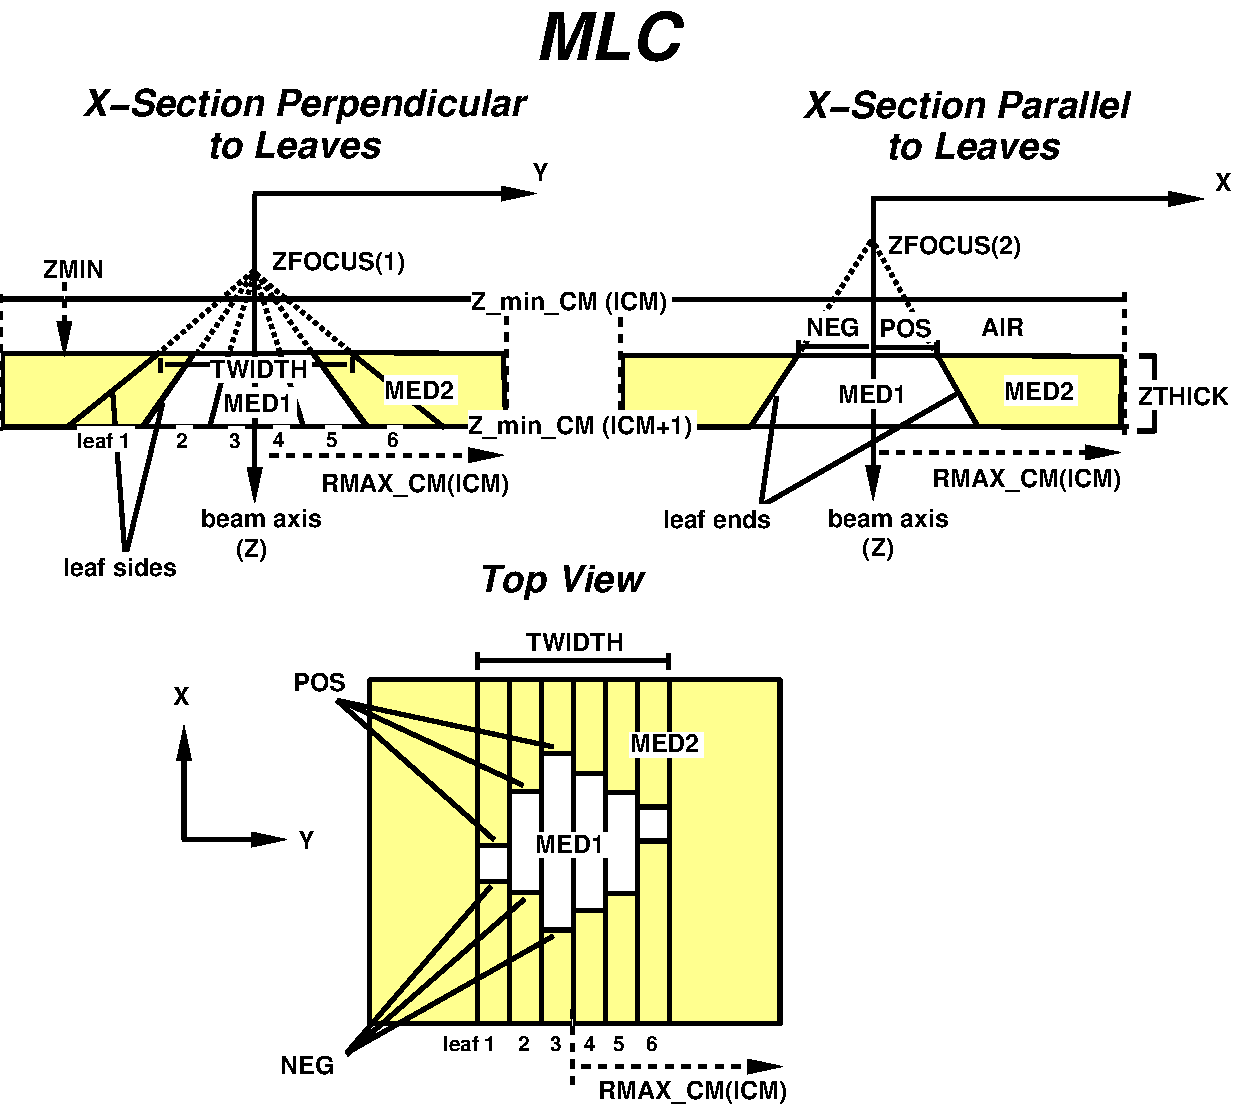
\includegraphics[height=12cm]{figures/mlcd}}
\end{htmlonly}
\end{center}
\caption[MLC CM geometry]
{An MLC component module with 6 leaves ({\tt NUM\_LEAF}=6) opening in the X
direction ({\tt IDMLFC}=1).  The cross-section perpendicular to the leaves
(in the Y direction) shows the total width of the leaves at
the top of the collimator, {\tt TWIDTH}.  The width of each leaf at the top
is {\tt TWIDTH}/{\tt NUM\_LEAF}.  Note that {\tt NUM\_LEAF} must be
an even number so that there is an equal number of leaves on either side
of the X axis.  The Y coordinates of the leaves
at the bottom of the collimator are calculated automatically so that
the tangents to the
side surfaces of the leaves all cross the Z-axis at Z={\tt ZFOCUS(1)}.  The
cross-section parallel to the leaves (in the X direction) shows the negative,
{\tt NEG},
and positive, {\tt POS}, coordinates of the opening in one leaf.
{\tt NEG} and {\tt POS} coordinates are input for every leaf.
The X coordinates
of the leaf openings at the bottom of the collimator are calculated
automatically so that the tangents to the leaf ends all cross the Z-axis at
Z={\tt ZFOCUS(2)}.  The
top view of the collimator shows how the collimator opening is composed
of the individual leaf openings.  {\tt MED1} defines the material in the collimator
opening and {\tt MED2} defines the material of the collimator leaves and body.
This example would be applicable to leaves opening
in the Y direction ({\tt IDMLFC}=0) by reversing the roles of X and Y.  Although this
particular example shows {\tt ZFOCUS} points that are $<$ {\tt ZMIN}, the {\tt ZFOCUS}
points can also be $>$ {\tt ZMIN}+{\tt ZTHICK}, in which case leaf surfaces angle
in towards the Z-axis with increasing Z.}
\label{fig_MLCD}
\end{figure}

%\setlength{\textheight}{9.0in}

\clearpage

The input format for MLC and an example input are given below.
\begin{small}
\index{MLC!inputs}
\input{./inputformats/MLC.inp}
\end{small}
\index{input file!for MLC}

%\setlength{\textheight}{10.0in}

%\clearpage

%\markboth{MLCQ Users Manual}{~~~~last edited 2004/11/19 20:21:18
%~~~~printed \today}

\subsubsection{MLCQ}
\label{mlcq}
\renewcommand{\rightmark}{MLCQ CM}
\index{MLCQ}
\index{multi-leaf collimator!MLCQ}
The MLCQ CM is used to model a focusing multi-leaf collimator
with rounded leaf
ends.  The collimator is similar to MLC with the exception that, rather
than specifying a Z focus for the leaf ends, the user specifies a radius
for the leaf ends and the Z position of the origin of this radius (\ie\ so
the leaf ends can be angled up or down).  The collimator opening is defined
by specifying the X or Y (depending on leaf orientation) origin of the
radius for the positive and negative portions of each leaf.

The first version of this CM, which was based on MLC, was coded by Hugo
Palmans and Kristiaan De Vlamynck of the University of Gent, Belgium.

\newpage
\begin{figure}[tp]
\begin{center}
\leavevmode
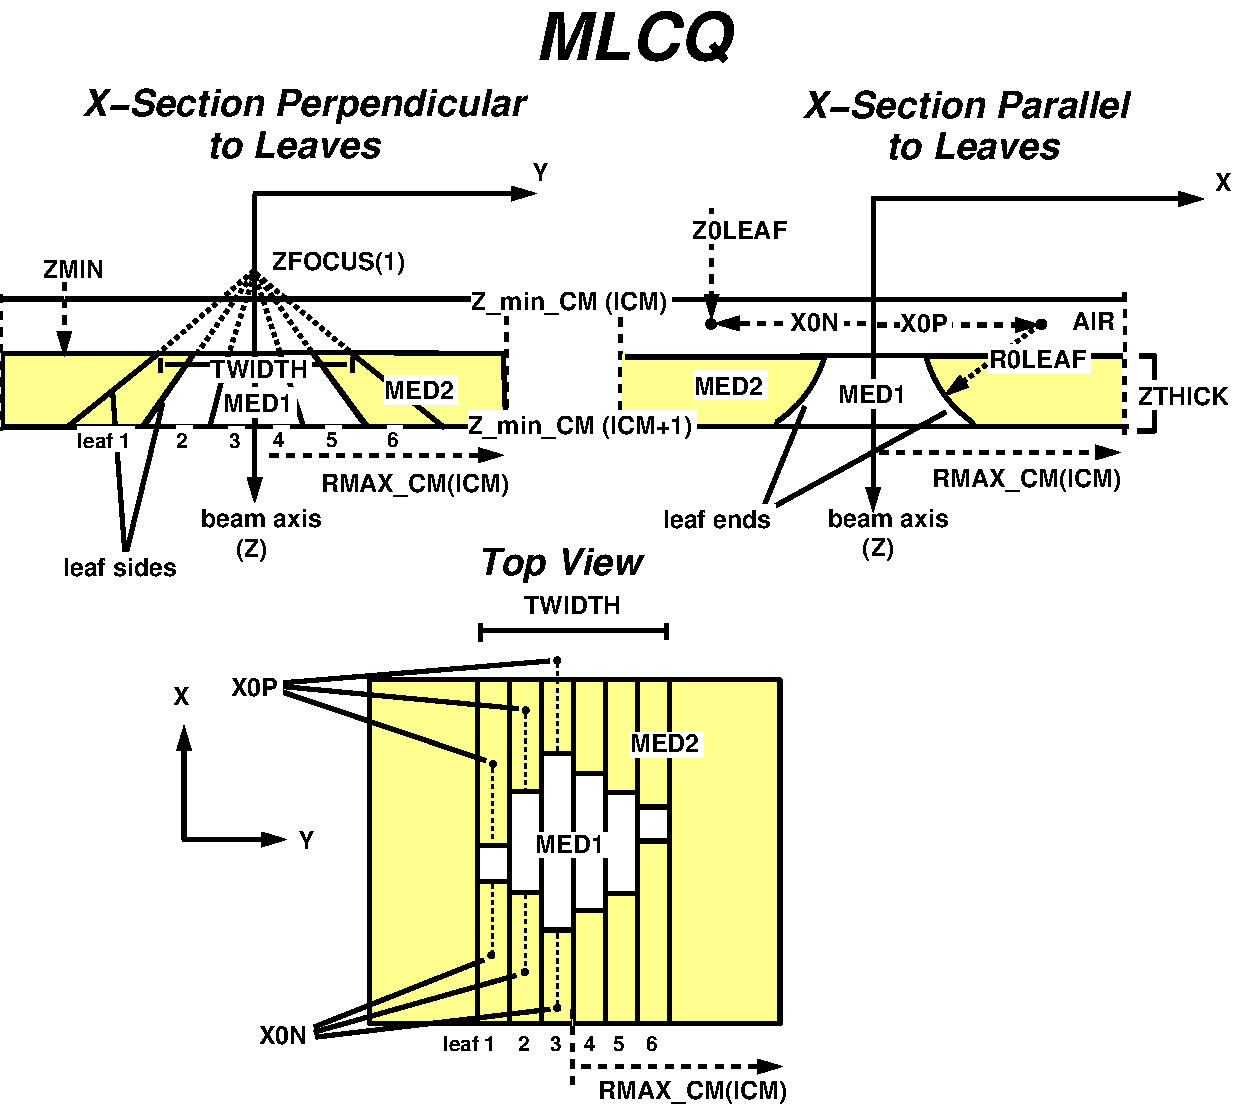
\includegraphics[height=13cm]{figures/mlcqd}
\end{center}
\caption[MLCQ CM geometry]
{An MLCQ component module with 6 leaves ({\tt NUM\_LEAF}=6) opening in the X
direction ({\tt IDMLFC}=1).  Parameters are similar to MLC with the
exception of those for the leaf ends.  The cross-section parallel to the leaves
shows how the rounded leaf ends are defined.  Basically, for each leaf, the user defines a circle
with radius {\tt R0LEAF} (the radius of the leaf ends), centred at
({\tt X0N},{\tt Z0LEAF}) for the negative portion of the leaf and
({\tt X0P},{\tt Z0LEAF}) for the positive portion of the leaf.  Note that {\tt X0N},{\tt X0P}
define X coordinates if the leaves are parallel to the X direction and Y coordinates if the
leaves are parallel to the Y direction.  Also note that {\tt Z0LEAF} applies to all leaves.
The rounded leaf end is then the arc
subtended by the intersection of this circle with {\tt ZMIN} and {\tt ZMIN + ZTHICK}.  The user
controls the angle of the leaf ends with respect to the Z axis using {\tt Z0LEAF} and the
dimensions of the leaf opening using {\tt X0N} and {\tt X0P}.
The top view shows that
{\tt ABS(X0N)} and {\tt ABS(X0P)} can be $>$ {\tt RMAX\_CM}, however the points of
intersection of the circle defining a leaf end with {\tt ZMIN} and {\tt ZMIN + ZTHICK} must
be within the boundaries of the CM or else the volume/mass of the collimator will be determined
incorrectly for dose calculations.}
\label{fig_MLCQD}
\end{figure}

%\setlength{\textheight}{9.0in}

\clearpage

The input format for MLCQ and an example input are given below.
\begin{small}
\index{MLCQ!inputs}
\input{./inputformats/MLCQ.inp}
\end{small}
\index{input file!for MLCQ}

%\setlength{\textheight}{10.0in}

%\clearpage

%\markboth{VARMLC Users Manual}{~~~~last edited 2004/11/19 20:21:18
%~~~~printed \today}

\subsubsection{VARMLC}
\label{varmlc}
\renewcommand{\rightmark}{VARMLC CM}
\index{multi-leaf collimator!VARMLC}
\index{VARMLC}
The VARMLC CM is used to model a focusing multi-leaf collimator
with either rounded leaf
ends or straight leaf ends with a Z focus.  The major difference between
VARMLC and MLC or MLCQ is that
VARMLC simulates the air gaps between leaves, the tongue-in-groove
mechanism by which adjacent leaves slide against each other, and the
driving screws at the top and bottom of each leaf used to open and close
the leaves.  VARMLC can also simulate leaves of different widths within
the same collimator.
In VARMLC the medium beyond the leaves in the direction perpendicular
to the leaves defaults to be the same as the medium in the leaf opening(s)
(ie AIR).  This is different from MLC and MLCQ in which the medium in this
region defaults to the leaf medium (ie solid).  This default can be changed
within the {\tt VARMLC\_cm.mortran} and {\tt VARMLC\_macros.mortran} codes.

The first version of this CM was coded by Ajay Kapur with Charlie Ma
at Stanford University.  The current version has significant
modifications.

\newpage
\begin{figure}[tp]
\begin{center}
\htmlimage{scale=2.0}
\leavevmode
\begin{latexonly}
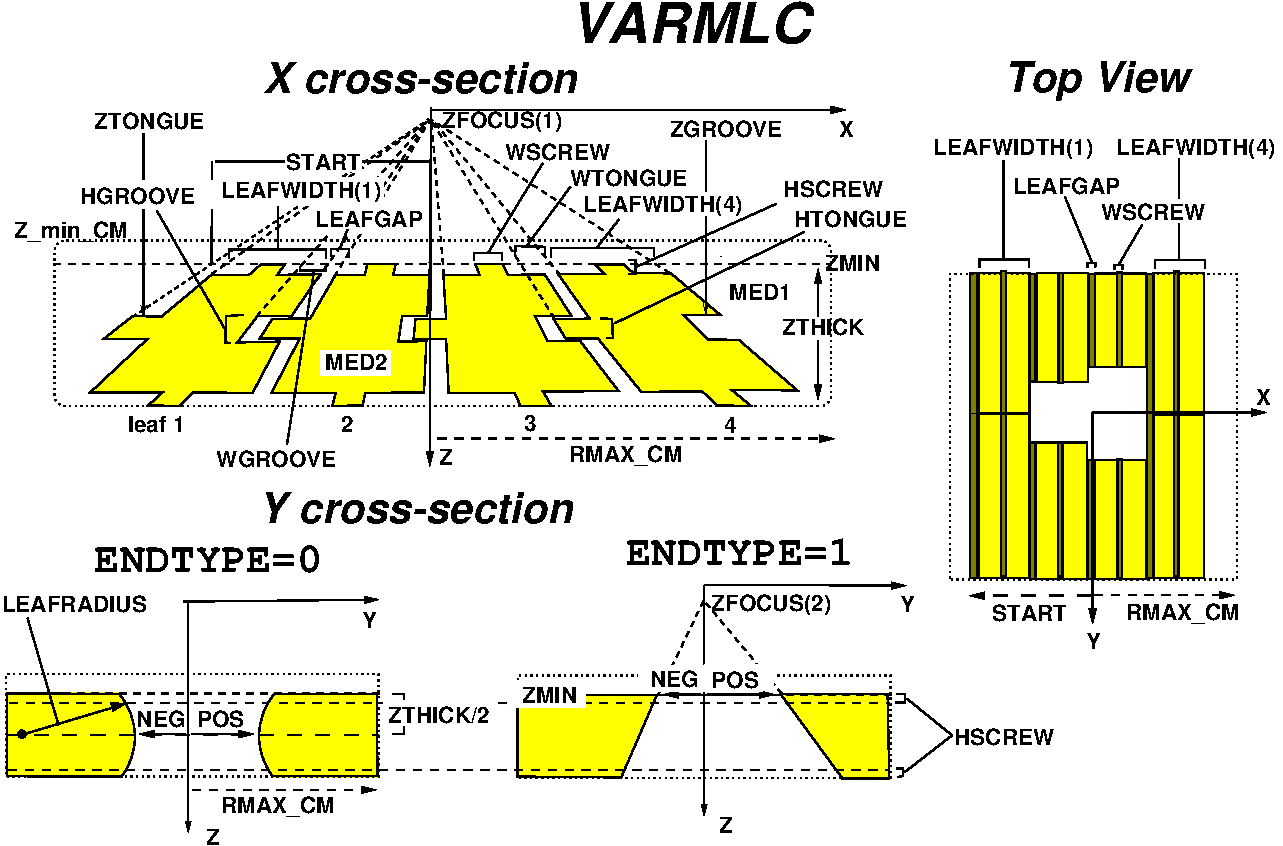
\includegraphics[width=18cm]{figures/varmlcd}
\end{latexonly}
\begin{htmlonly}
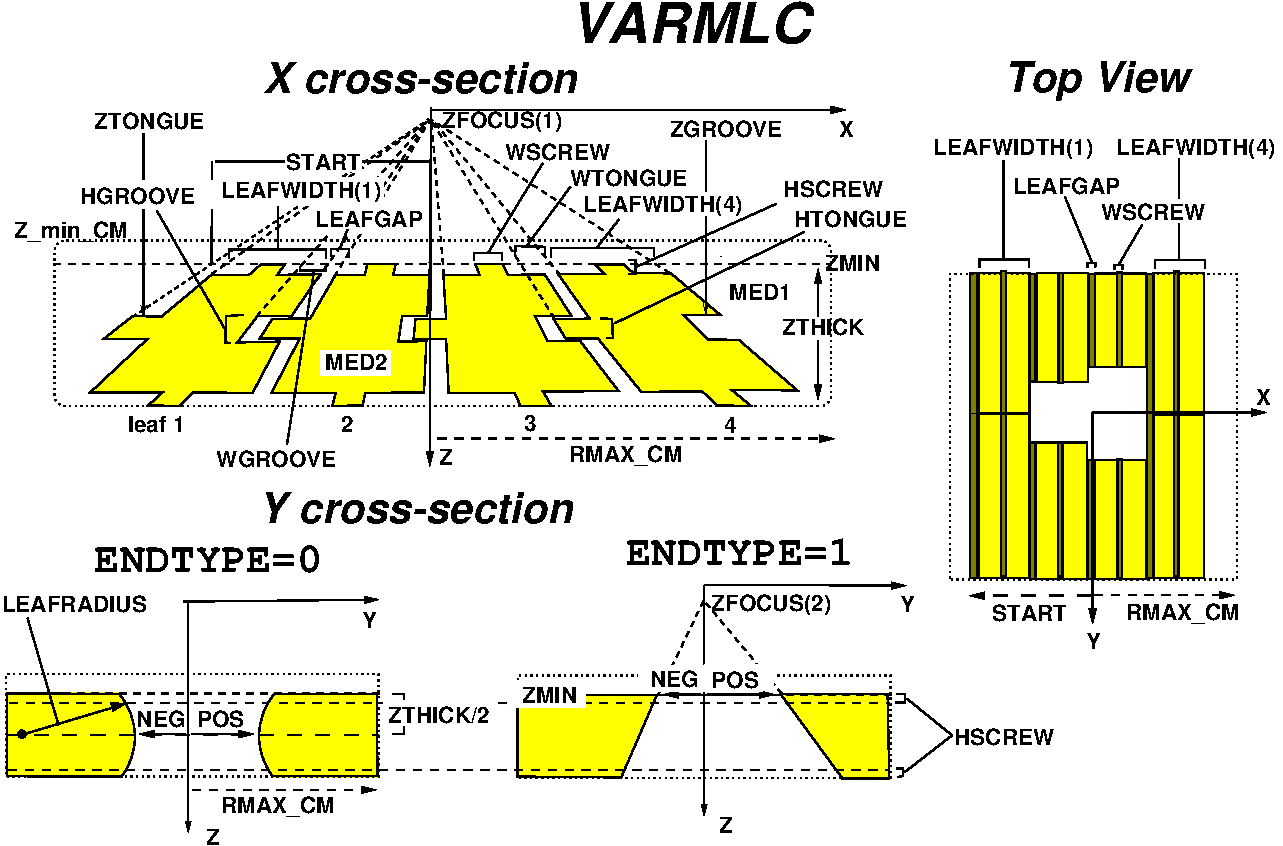
\includegraphics[width=13cm]{figures/varmlcd}
\end{htmlonly}
\end{center}
\caption[VARMLC CM geometry]
{A VARMLC component module with 4 leaves ({\tt NUM\_LEAF}=4) opening in the Y
direction ({\tt ORIENT}=0).  The X cross-section (perpendicular to
the leaf direction) shows the widths of the leaves
({\tt LEAFWIDTH(1)...LEAFWIDTH(4)}) and the dimensions of
the leaf gap ({\tt LEAFGAP}), tongue-in-groove mechanism ({\tt WGROOVE, HGROOVE,
WTONGUE, HTONGUE}) and the driving screws ({\tt WSCREW, HSCREW}) as input by
the user.  The user also sets the position of the top of the tongue,
{\tt ZTONGUE},
and the top of the groove, {\tt ZGROOVE}, with the restriction that the tongue
and groove cannot overlap.  If {\tt ZTONGUE}={\tt ZGROOVE}=0 then
the tongue and groove are centred at {\tt Z = ZMIN + ZTHICK/2}.
For restrictions on leaf gap and tongue-in-groove inputs, see the detailed description
of input parameters below.
Note that all leaf side surfaces are focused at {\tt ZFOCUS(1)}
and that horizontal dimensions ({\tt WGROOVE, WTONGUE, WSCREW, START}) are all given
at {\tt ZMIN}.
Due to {\tt LEAFGAP} and varying {\tt LEAFWIDTH} the leaves may not be
symmetric about the Z axis, although {\tt START}
can be set to give approximate symmetry. Also note that the medium
in regions beyond the leaves perpendicular to the leaf direction defaults to {\tt MED1},
the medium of the openings and air gaps.  Y cross-sections are shown for leaves
with rounded ends ({\tt ENDTYPE=0}) and straight ends ({\tt ENDTYPE=1}).  For rounded
ends, the user inputs the radius of the ends ({\tt LEAFRADIUS}) and, for each leaf,
the minimum and maximum coordinates of the leaf opening at {\tt Z = ZMIN + ZTHICK/2}
({\tt NEG, POS}).  The end radius is always assumed to originate at
{\tt Z = ZMIN + ZTHICK/2}.  For straight leaf ends, the user inputs the Z focus of the
ends ({\tt ZFOCUS(2)}) and, for each leaf, the minimum and maximum coordinates of
the opening at {\tt Z = ZMIN} ({\tt NEG, POS}).}
\label{fig_VARMLCD}
\end{figure}

%\setlength{\textheight}{9.0in}

\clearpage

The input format for VARMLC and an example input are given below.
\begin{small}
\index{VARMLC!inputs}
\input{./inputformats/VARMLC.inp}
\end{small}
\index{input file!for VARMLC}

\index{IGNOREGAPS!option in VARMLC}
Note that VARMLC has an additional input, {\tt IGNOREGAPS}, appearing on
the same line as {\tt ECUT}, {\tt PCUT} etc for the leaves.  This input
increases the efficiency of range rejection for particles in the
leaves.  If {\tt IGNOREGAPS} is set to 1, then all air gaps within the leaves
(ie gaps between leaves and the Z-directional gaps caused by the presence
of carriage screws) are ignored when doing charged particle range rejection
provided that the particle is in the leaves and satisfies:\\
~~~\\
particle X $<$ minimum X of all leaf openings (excluding rounded or focused leaf end) or\\
particle X $>$ maximum X of all leaf openings (excluding leaf end)\\
~~\\
if the leaves are parallel to X ({\tt ORIENT}=1) or:\\
~~~\\
particle Y $<$ minimum Y of all leaf openings (excluding leaf end) or\\
particle Y $>$ maximum Y of all leaf openings (excluding leaf end)\\
~~\\
if the leaves are parallel to Y ({\tt ORIENT}=0).  Exact transport is
preserved in the shaped leaf ends (rounded or focused) by excluding them
from the volume in which air gaps are ignored.  This is important, since
the leaf ends define the field shape and particles interacting in the ends are
more likely to reach the field at the SSD.

Use of the {\tt IGNOREGAPS} option can reduce the CPU time spent in
VARMLC by a factor of 2.  However, if the multi-leaf collimator you
are modeling has significant air gaps between leaves, we recommend
that you run with this option turned off
(ie {\tt IGNOREGAPS} set to 0; the default) so that there is exact
transport everywhere.


\clearpage

%\markboth{MLCE Users Manual}{~~~~last edited 2004/11/19 20:21:18
%~~~~printed \today}

\subsubsection{MLCE}
\label{mlce}
\renewcommand{\rightmark}{MLCE CM}
\index{multi-leaf collimator!MLCE}
\index{MLCE}
The MLCE CM is used to model multi-leaf collimators specific for
Elekta machines.  Instead of
specifying a tongue-and-groove, the user specifies the dimensions of
interlocking steps typical of this class of MLC.  All leaves
have identical cross-sections, and leaf sides
are focused (always to Z=0) by tilting each leaf about an
axis that runs parallel to the leaf opening direction
and along the centre of its top surface.  The entire leaf bank can also
be rotated in a plane
perpendicular to the leaf opening direction by a user-specified angle.
As in
VARMLC, the medium beyond the leaves in the direction perpendicular
to the leaves defaults to be the same as the medium in the leaf opening(s)
(ie AIR).

This CM was mostly coded by Nick Reynaert at the University of Ghent.
There have been some modifications of inputs and some small bugs were
fixed.

\begin{figure}[htpb]
\begin{center}
\htmlimage{scale=2.0}
\leavevmode
\begin{latexonly}
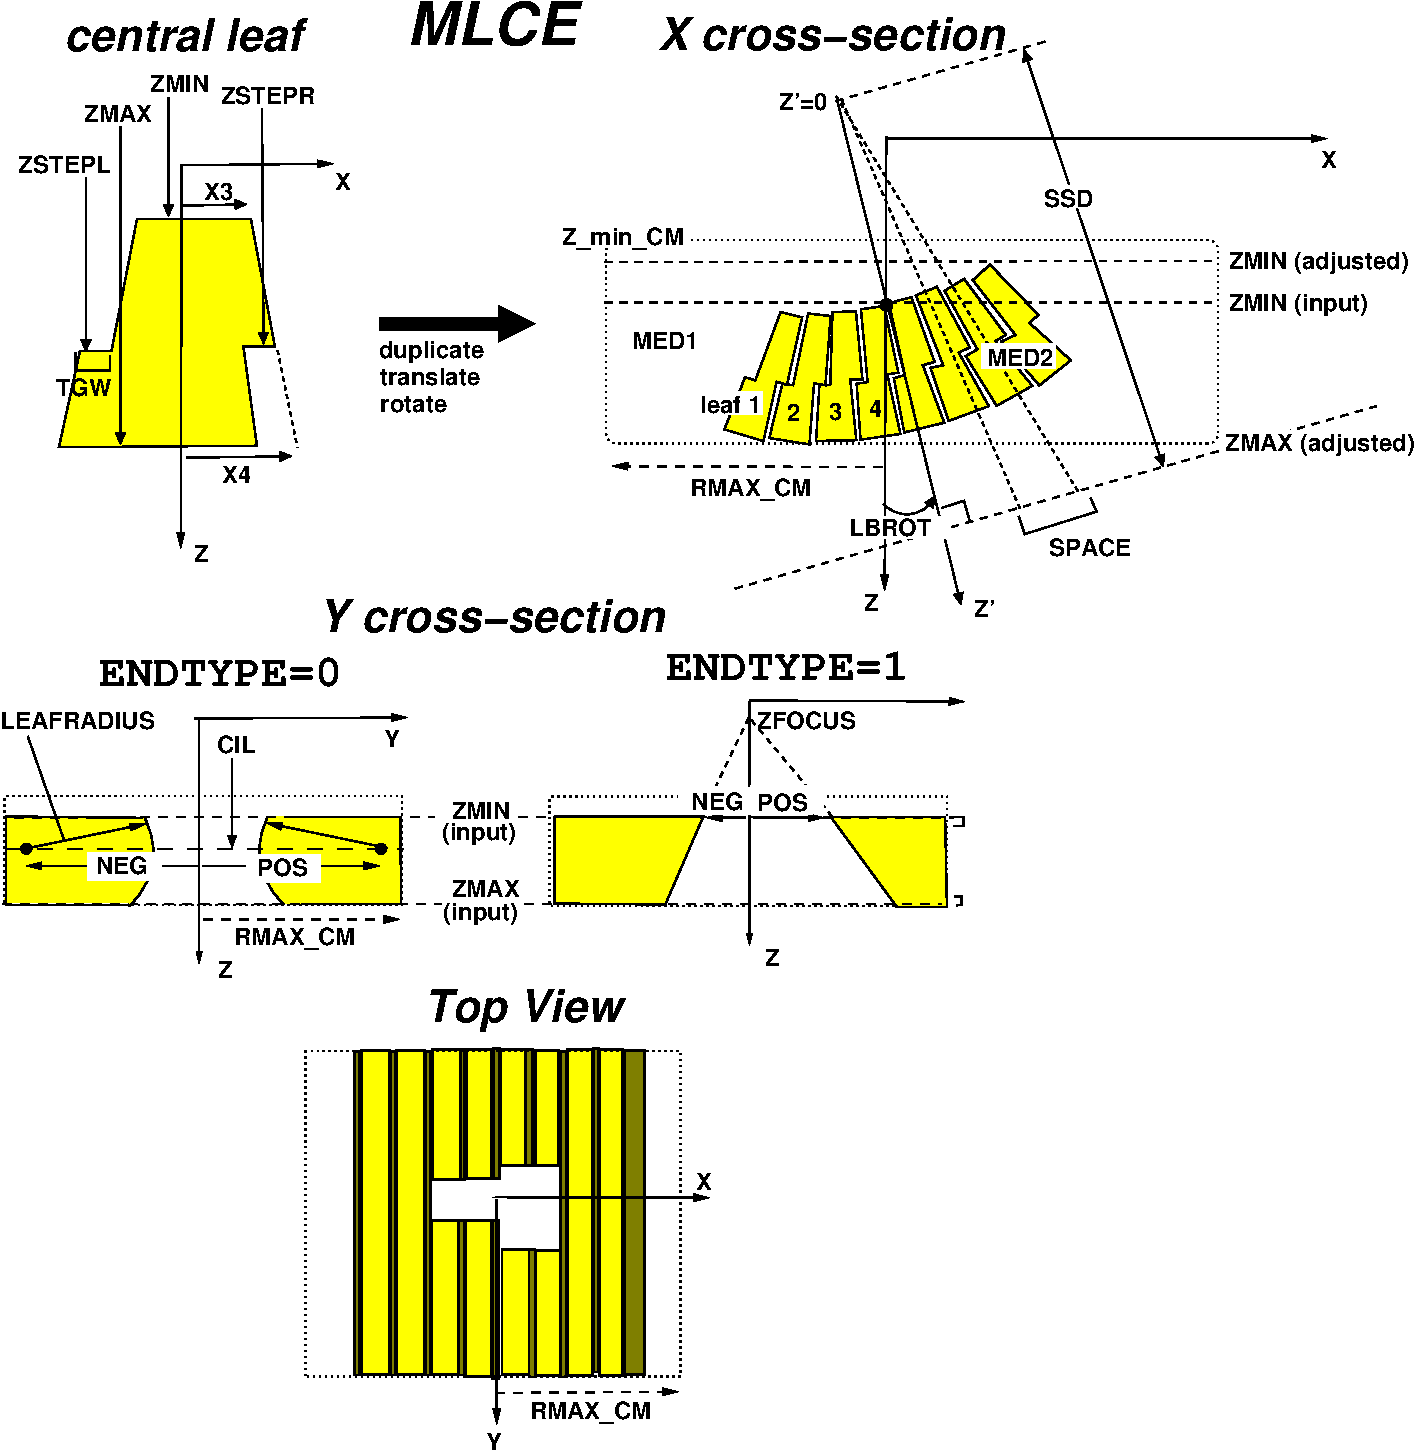
\includegraphics[width=18.5cm]{figures/mlced}
\end{latexonly}
\begin{htmlonly}
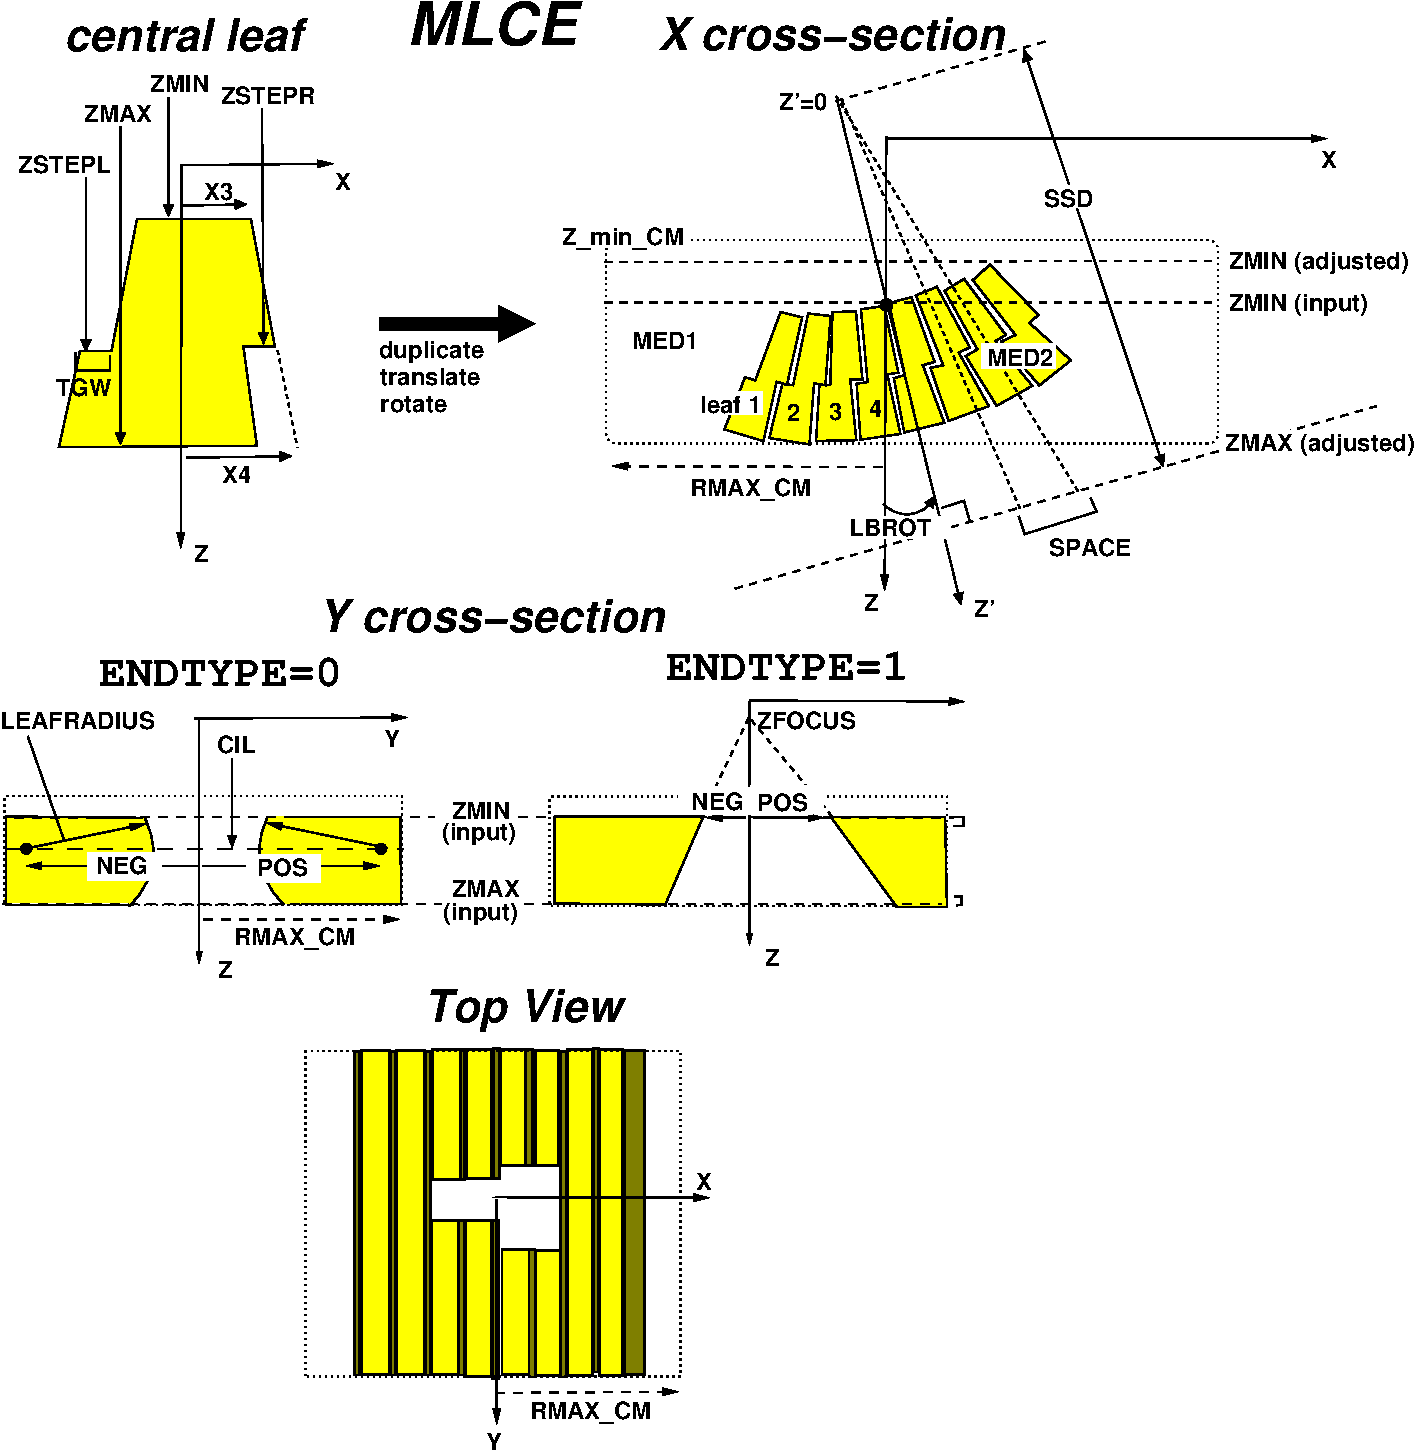
\includegraphics[width=13cm]{figures/mlced}
\end{htmlonly}
\end{center}
\caption[MLCE CM geometry]
{Example MLCE with 8 leaves ({\tt NUM\_LEAF}=8) opening in the Y
direction ({\tt ORIENT}=0) and with a leaf bank rotation angle
of {\tt LBROT}.  The figure also shows the cross-section
of the imaginary ``central leaf'', used to create the leaves, and
the two possible leaf end types: cylindrical ({\tt ENDTYPE}=0) and
straight ({\tt ENDTYPE}=1).  See text for more details.}
\label{mlce_fig}
\end{figure}

Details of MLCE are shown in Figure~\ref{mlce_fig}.  All leaves have
identical cross-sections, which are defined using an imaginary
``central leaf''.  For this leaf,
the user specifies the 4 points defining the cross-section (which is symmetric
about X=0 if the steps are ignored),
{\tt X3}, {\tt ZMIN}, {\tt X4}, {\tt ZMAX}, the Z positions of the left and right
steps, {\tt ZSTEPL},{\tt ZSTEPR}, and the step width, {\tt TGW}.   Note that
{\tt ZSTEPL} must be $>${\tt ZSTEPR} for the steps to fit into one another
once the leaves are generated.  The central leaf is then duplicated
{\tt NUM\_LEAF} times, and each leaf is rotated/translated in the
X ({\tt ORIENT}=0) or Y ({\tt ORIENT}=1) direction.
Rotation angle and translation distance are determined by user
inputs which define the spacing between the
centres of the leaf cross-sections, {\tt SPACE},
as projected down to {\tt SSD} and the requirement that the leaf sides
focus to Z=0.   Leaves are first rotated about the X=0 ({\tt ORIENT}=0)
or Y=0 ({\tt ORIENT}=1), Z={\tt ZMIN} using:
\begin{equation}
rotation=
\begin{cases}
ATAN\left[-\left(2I-1\right)\left(\frac{SPACE}{2}\right)\left(\frac{ZMIN}{SSD}\right)\right] &
\text{for 1$\leq I\leq\frac{NUM\_LEAF}{2}$},\\
ATAN\left[\left(2I-1\right)\left(\frac{SPACE}{2}\right)\left(\frac{ZMIN}{SSD}\right)\right] &
\text{for $\frac{NUM\_LEAF}{2}+1\leq I\leq NUM\_LEAF$}.
\end{cases}
\end{equation}
Then they are translated in the X ({\tt ORIENT}=0) or Y
({\tt ORIENT}=1) direction using:
\begin{equation}
translation=
\begin{cases}
-\left(2I-1\right)\left(\frac{SPACE}{2}\right)\left(\frac{ZMIN}{SSD}\right) &
\text{for 1$\leq I\leq\frac{NUM\_LEAF}{2}$},\\
\left(2I-1\right)\left(\frac{SPACE}{2}\right)\left(\frac{ZMIN}{SSD}\right) &
\text{for $\frac{NUM\_LEAF}{2}+1\leq I\leq NUM\_LEAF$}.
\end{cases}
\end{equation}
Note the restriction that {\tt NUM\_LEAF} must be an even number.
After the leaves have been rotated/translated according to the above equations,
their cross-sections are symmetric about the Z axis.

The user also has
the option to rotate the entire leaf bank about the axis
X=0 ({\tt ORIENT}=0) or Y=0 ({\tt ORIENT}=1), Z={\tt ZMIN} by angle
{\tt LBROT} (which must be specified in radians).  This rotates the
central axis of the leaves (ie the axis along which they are focused) from
Z to Z', as shown in Figure~\ref{mlce_fig}.  Rotation of the leaves,
both individually and of the entire leaf bank, requires automatic resetting
of {\tt ZMIN} and {\tt ZMAX}, shown as {\tt (adjusted)} values in the figure.

Figure~\ref{mlce_fig} also shows the two types of leaf ends possible with
MLCE.
Cylindrical leaf ends ({\tt ENDTYPE}=0) are defined by
the radius, {\tt LEAFRADIUS}, and Z position,
{\tt ZCIL}, of the cylinder describing the ends.
Leaf openings are specified by the
X ({\tt ORIENT}=1) or Y ({\tt ORIENT}=0)
coordinates of the cylinder origins for the positive
({\tt POS}) and negative ({\tt NEG}) portions of the leaf.
Straight leaf ends ({\tt ENDTYPE}=1) are angled according to
the user-input {\tt ZFOCUS}, and leaf openings are specified by the
X {\tt ORIENT}=1) or Y ({\tt ORIENT}=0)
coordinates of the ends of the positive ({\tt POS}) and
negative ({\tt NEG}) portions of the leaf at Z={\tt ZMIN}.

Note that MLCE input allows you to apply values of {\tt POS} and
{\tt NEG} to groups of adjacent leaves, which can save tedious input
in the case where many adjacent leaves have the same opening
coordinates.  See the input description below for more details.

The input format for MLCE and an example input are given below.
\begin{small}
\index{MLCE!inputs}
\input{./inputformats/MLCE.inp}
\end{small}
\index{input file!for MLCE}

\clearpage

\renewcommand{\rightmark}{SYNCMLCE CM}
\subsubsection{SYNCMLCE}
\index{SYNCMLCE}

SYNCMLCE is a synchronized version of MLCE (See Section~\ref{mlce} above) that can be used to simulate
changing leaf opening coordinates during an accelerator simulation.  Similar to
DYNVMLC (See Section~\ref{dynvmlcsect}), motion of opening coordinates
can be simulated in ``dynamic'' or ``step-and-shoot'' mode.  In dynamic mode,
the leaves move while the beam is on, while in step-and-shoot mode, motion of
the leaves occurs while the beam is off.  When used in either mode, leaf
opening coordinates in SYNCMLCE can be synchronized with the settings of
any other synchronized CMs (SYNCJAWS, SYNCVMLC and SYNCHDMLC) in the accelerator
and with the motion of source 20 (synchronized phase space) or source 21
(synchronized BEAM treatment head) in DOSXYZnrc\cite{Wa05}.  SYNCMLCE was
contributed by Lobo \& Popescu\cite{LP10}.

Inputs to SYNCMLCE are similar to that for MLCE with the exception that,
on the same line as {\tt ORIENT}, defining the leaf orientation, there is
an input, {\tt MODE}, defining the dynamic mode of SYNCMLCE.  If
{\tt MODE}=0, then SYNCMLCE is used in static mode, and the inputs
are identical to MLCE.  If {\tt MODE}=1 (``dynamic'') or 2 (``step-and-shoot''), however,
instead of reading the leaf opening coordinates from the BEAMnrc input file, SYNCMLCE reads
the opening coordinates for {\tt NFIELD} multiple fields from a separate file.

\index{INDEX(I)}\index{muIndex(I)}
The format of the file of leaf opening coordinates is identical to that
used for DYNVMLC, SYNCVMLC and SYNCHDMLC and is given in more detail in
Section~\ref{dynvmlcsect} below.  In the case of SYNCMLCE, the input parameter, {\tt INDEX(I)}, defining
the cumulative probability of all fields up to and including field {\tt I}, is interpreted as {\tt muIndex(I)},
the fraction of monitor units delivered up to and including field {\tt I}.

\index{MU\_RND}
\index{muIndex}
\index{SYNCMLCE!calculating leaf opening coordinates}
For each primary history, a random number, {\tt MU\_RND}$\in[$0,1$]$, is compared to the
{\tt muIndex(I)} and is used to determine which field to use and, in ``dynamic'' mode, to calculate
the leaf opening coordinates.  A more detailed description of how this is done is given
in the documentation for DYNVMLC (Section~\ref{dynvmlcsect}). The equation used by SYNCMLCE to calculate
leaf opening coordinates in ``dynamic'' mode is the same as Equation (9), with {\tt INDEX} replaced
by {\tt muIndex} and {\tt RNDM1} replaced by {\tt MU\_RND}.

If SYNCMLCE is the only synchronized
CM in the accelerator, then {\tt MU\_RND} is chosen by SYNCMLCE and used only by SYNCMLCE.  However,
if there are other synchronized CMs in the accelerator, then {\tt MU\_RND} is generated by the
first (most upstream) synchronized CM and then passed down to all downstream synchronized CMs.  Thus,
the motion of SYNCMLCE leaves can be synchronized with the coordinates of all other synchronized CMs in
the accelerator.

\index{DOSXYZnrc sources 20 and 21}
Furthermore, if the accelerator is compiled as a shared library, then the value of {\tt MU\_RND} used
in SYNCMLCE is also passed on to DOSXYZnrc simulations
when using DOSXYZnrc sources 20 (synchronized phase space) or 21 (synchronized BEAM treatment head simulation).  This
allows the motion of these dynamic sources to be synchronized with that of the leaf openings.  See the
DOSXYZnrc Users Manual\cite{Wa05} for more details.

An example of a file specifying dynamic leaf settings for SYNCMLCE
is included with the distribution.  This file is {\tt \$OMEGA\_HOME/beamnrc/CMs/sample\_syncmlce.sequence}.

The input format for SYNCMLCE and an example input are shown below:
\begin{small}
\index{SYNCMLCE!inputs}
\input{./inputformats/SYNCMLCE.inp}
\end{small}
\index{input file!for SYNCMLCE}


\clearpage

%\markboth{DYNVMLC Users Manual}{~~~~last edited 2004/11/19 20:21:18
%~~~~printed \today}
\renewcommand{\rightmark}{DYNVMLC CM}
\subsubsection{DYNVMLC}
\label{dynvmlcsect}
\index{DYNVMLC}
DYNVMLC is a CM specifically designed to model the Varian Millenium
multi-leaf collimator.  The code is based on VARMLC.  The user specifies
cross-sections perpendicular to the leaf opening direction for the 3 leaf
types (FULL, TARGET and ISOCENTER leaves) found in the mlc.  Each leaf
in the leaf bank (usually comprising 120 leaves in all) is assigned
a type, with TARGET/ISOCENTER leaves always occuring in pairs.  The user
also specifies a Z focal point for
the leaf sides and either the radius (for cylindrical ends) or Z focal point
(for straight ends)
for the leaf ends. Note that DYNVMLC leaf cross sections are more complex than those in the
VARMLC CM.

DYNVMLC allows the simulation of multiple fields
(where a field is defined by a complete set of leaf openings)
during a single run.  Leaf opening coordinates can be simulated changing
while the beam is on (dynamic, or {\tt MODE=1}, simulation) or while
the beam is off (step-and-shoot, or {\tt MODE=2}, simulation).
For these simulations, the user must supply a file
containing the leaf opening data for each field
and the relative intensity of each field.  Alternatively, DYNVMLC can be
used to simulate a fixed set of leaf opening coordinates for the
entire run (static, or {\tt MODE=0}, simulation).

DYNVMLC was originally coded by Emily Heath at McGill University.
There have been some modifications of inputs and some bugs were
fixed.

\begin{figure}[htpb]
\begin{center}
\vspace*{-0.7cm}
\htmlimage{scale=2.0}
\leavevmode
\begin{latexonly}
\hspace*{-1cm}
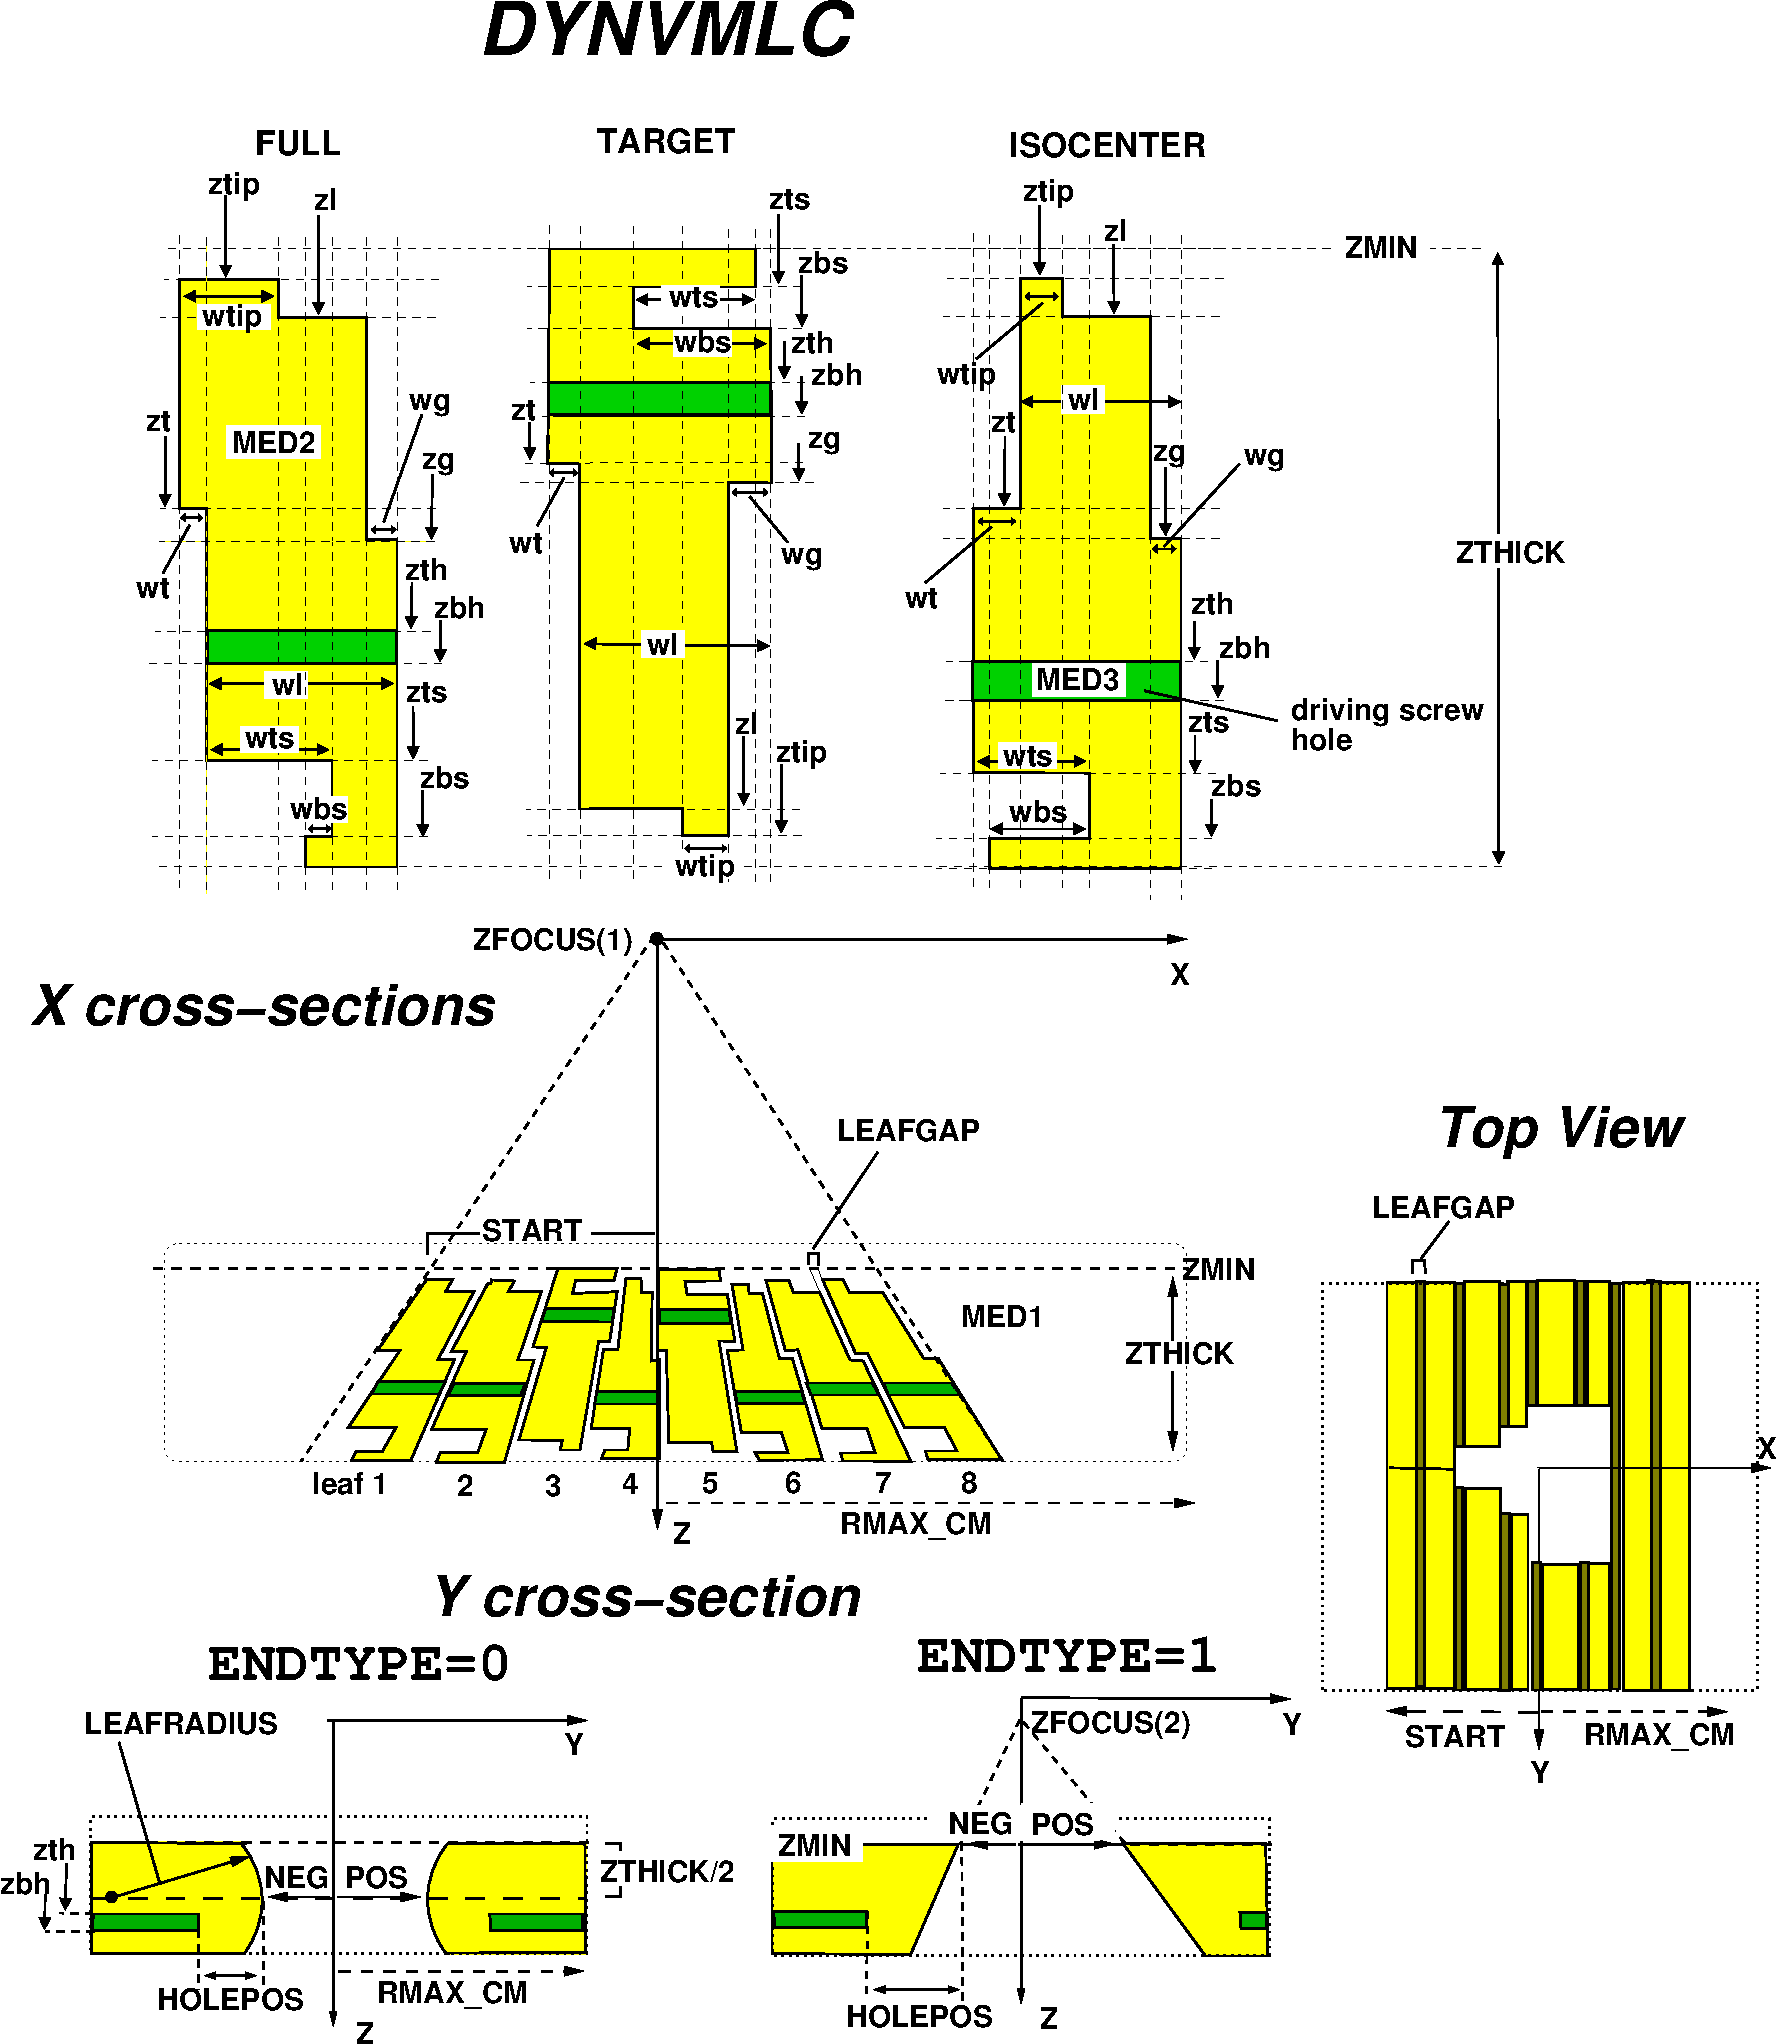
\includegraphics[width=18.5cm]{figures/dynvmlcd}
\end{latexonly}
\begin{htmlonly}
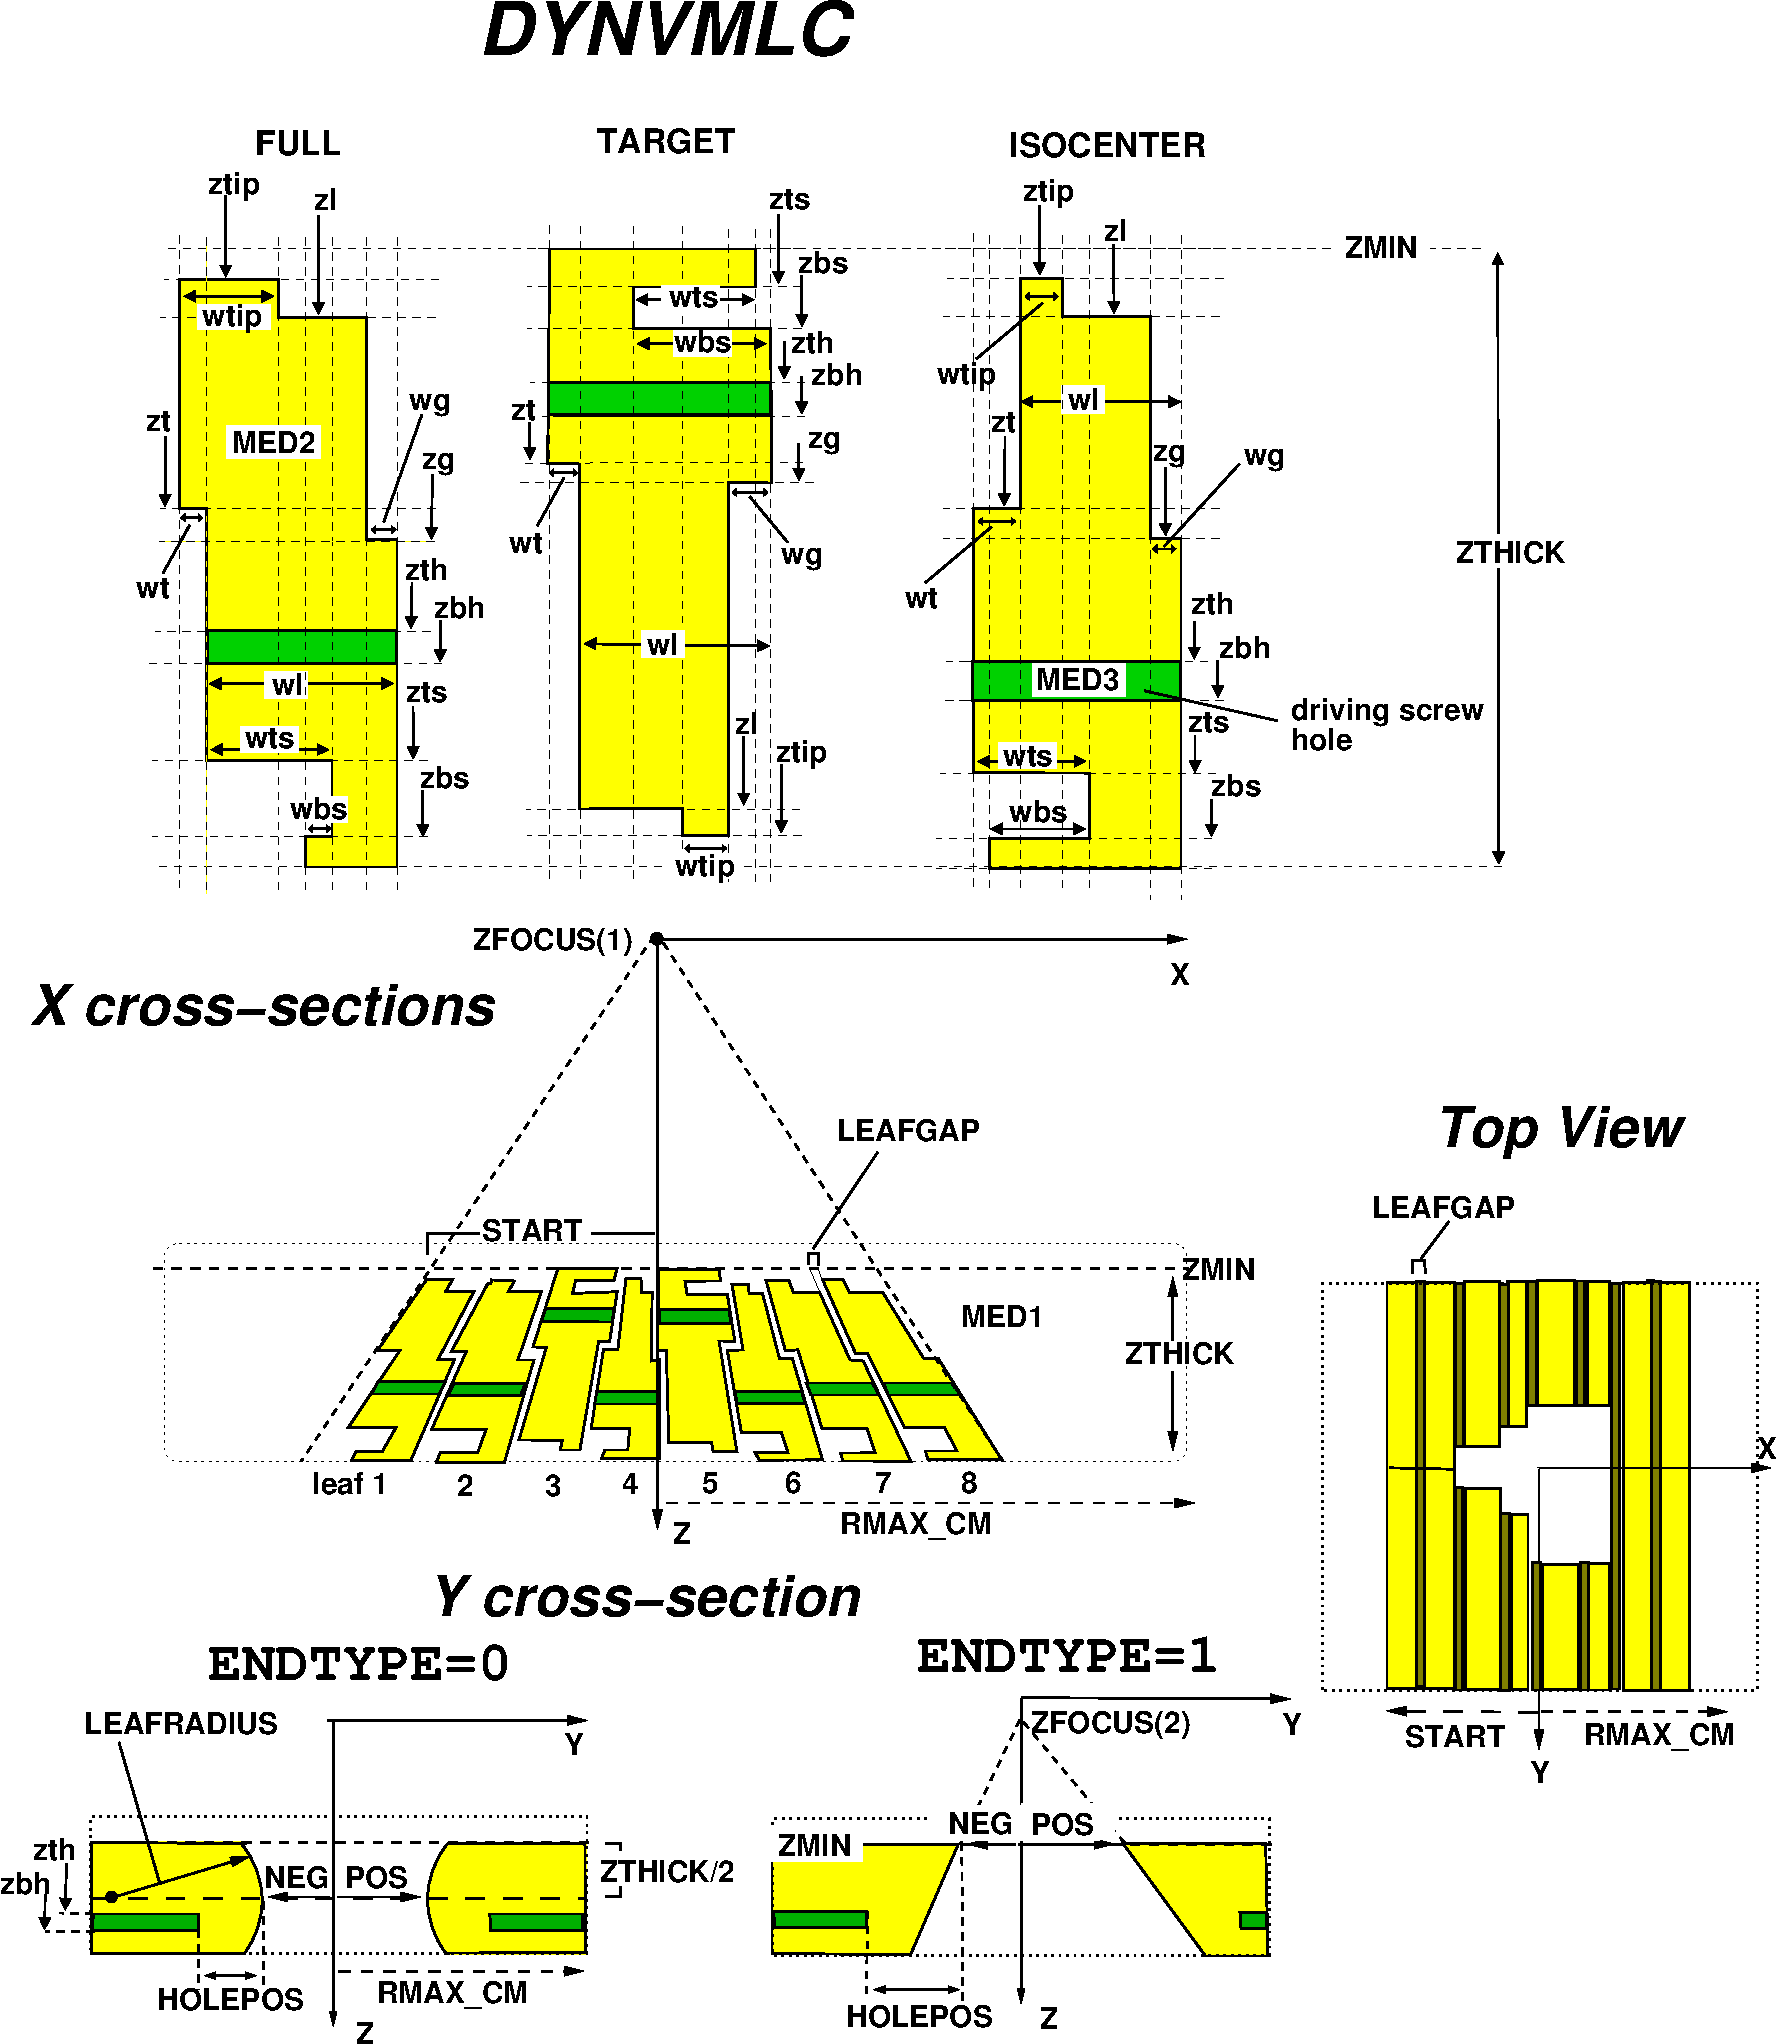
\includegraphics[width=13cm]{figures/dynvmlcd}
\end{htmlonly}
\end{center}
\vspace*{-0.7cm}
\caption[DYNVMLC CM geometry]
{Example DYNVMLC with 8 leaves ({\tt NUM\_LEAF}=8) opening in the Y
direction ({\tt ORIENT}=0).  At the top of the figure
are detailed X cross-sections of the
3 leaf types, FULL, TARGET and ISOCENTER, showing the dimensions that the
user must input.  The dimension labels are explained in the text below.
The Y cross-section shows the two possible leaf end types: cylindrical ({\tt ENDTYPE}=0) and
straight ({\tt ENDTYPE}=1).}
\label{dynvmlc_fig}
\end{figure}

\index{FULL leaf! in DYNVMLC}
\index{TARGET leaf! in DYNVMLC}
\index{ISOCENTER leaf! in DYNVMLC}
Figure~\ref{dynvmlc_fig} shows an example DYNVMLC with 8 leaves
({\tt NUM\_LEAF}=8) opening in the Y direction ({\tt ORIENT}=0).  The
X cross-sections of the 3 leaf types, along with the dimensions that
you must specify, are shown in detail at the top.  The meanings of the
labels are shown in Table~\ref{dynvmlc_tab}.
\begin{table}[htb]
\caption{Meaning of labels in Figure~\ref{dynvmlc_fig}.}
\hspace*{-0.5cm}\begin{tabular}{llll}
\\
& \multicolumn{3}{c}{Leaf Type}\\
& \multicolumn{3}{c}{~~~}\\
& ~~~~FULL & ~~~~TARGET & ~~~~ISOCENTER \\
\hline
\multicolumn{4}{l}{{\bf widths:}} \\
{\tt wl} & leaf (excl. tongue) & leaf (excl. tongue) & leaf (excl. tongue)\\
{\tt wt} & tongue & tongue & tongue\\
{\tt wg} & groove & groove & groove\\
{\tt wtip} & tip at top of leaf & tip at bottom of leaf & tip at top of leaf\\
{\tt wts} & top support rail & top support rail & top support rail\\
{\tt wbs} & bottom support rail & bottom support rail & bottom support rail\\
\hline
\multicolumn{4}{l}{{\bf Z positions:}} \\
{\tt ztip} & top of tip & bottom of tip & top of tip\\
{\tt zl} & top of leaf & bottom of leaf & top of leaf\\
{\tt zt} & bottom of tongue & bottom of tongue & top of tongue\\
{\tt zg} & bottom of groove & top of groove & bottom of groove\\
{\tt zth} & top of driving screw hole & top of driving screw hole & top of driving screw hole\\
{\tt zbh} & bottom of driving screw hole & bottom of driving screw hole & bottom of driving screw hole\\
{\tt zts} & top of support rail & top of support rail & top of support rail\\
{\tt zbs} & bottom of support rail & bottom of support rail & bottom of support rail\\
\end{tabular}
\label{dynvmlc_tab}
\end{table}

FULL and ISOCENTER leaves extend from {\tt ztip} to {\tt ZMIN+ZTHICK}, while
TARGET leaves extend from {\tt ZMIN} to {\tt ztip}.  For each leaf, you
must also specify
the Z dimensions of a driving screw hole (filled with {\tt MED3}) that
spans the entire width of the leaf cross-section.  When specifying the
cross-sections of each leaf type, the grid lines shown in
Figure~\ref{dynvmlc_fig} must not change order, however they can overlap.
This means, for example, that when specifying the FULL leaf dimensions
{\tt zt} $\leq$ {\tt zg}, {\tt wt} $\leq$ {\tt wtip} $\leq$ {\tt wt + wts - wbs}, etc.  Also, Z positions of tongues and grooves must allow leaves to fit
together in the following
combinations: FULL/FULL (ie {\tt zt} $\leq$ {\tt zg}), FULL/TARGET
(ie {\tt zg}$_{FULL}$ $\geq$ {\tt zt}$_{TARGET}$), TARGET/ISOCENTER
(ie {\tt zg}$_{TARGET}$ $\leq$ {\tt zt}$_{ISOCENTER}$), ISOCENTER/TARGET
(ie {\tt zg}$_{ISOCENTER}$ $\geq$ {\tt zt}$_{TARGET}$)
and ISOCENTER/FULL (ie {\tt zg}$_{ISOCENTER}$ $\geq$ {\tt zt}$_{FULL}$).
All of these requirements put fairly tight restrictions on cross-section
dimensions.

Not shown in the leaf cross-sections is the distance, {\tt HOLEPOS},
between the leaf end and the end of the driving screw hole in the
leaf opening direction.  This must also be specified for each leaf type.

Once you have specified the cross-sections for the 3 leaf types, then you
must assign a type to each leaf in the leaf bank.  Since TARGET/ISOCENTER
leaves must always occur in pairs (with the TARGET leaf on the
negative X side if {\tt ORIENT}=0 or on the negative Y side if
{\tt ORIENT}=1), you really only have a choice of
two leaf types: 1. FULL leaf or 2. TARGET/ISOCENTER pair.  You can also specify
the number of adjacent leaves that have the same type so that you do not have
to input the type for each leaf or leaf pair separately.  In the example shown
in Figure~\ref{dynvmlc_fig}, leaves 1,2,7,8 are FULL (type 1) and
leaves 3-6 are TARGET/ISOCENTER pairs (type 2).

The X cross-section of the entire leaf bank shows how the different leaf types
fit together with interlocking steps and with an air gap between each leaf
specified by the {\tt LEAFGAP} input.  The negative-most leaf begins at
X={\tt START}.  All leaf sides are focused on
the Z axis at the user-specified focal point, {\tt ZFOCUS(1)}.  The focusing
of leaf sides means that leaf widths are not uniform from leaf top to bottom
(although in a realistic case, where the MLC is close to the SSD and
{\tt ZFOCUS(1)}=0, the variation in widths will be slight), and it is important
to note that all X ({\tt ORIENT}=0) or Y ({\tt ORIENT}=1) dimensions
 that you input (whether they be widths for the individual leaf types
or dimensions relevant to the entire leaf bank,
such as {\tt LEAFGAP} or {\tt START}) are specified at {\tt ZMIN}.

The Y cross-section in Figure~\ref{dynvmlc_fig} shows the
two possible leaf end types: cylindrical ({\tt ENDTYPE}=0) and
straight focused ({\tt ENDTYPE}=1).  Cylindrical leaf ends have radius
{\tt LEAFRADIUS} with the origin of the radius at
Z={\tt ZMIN}+{\tt ZTHICK}/2 (ie at the mid-point of the leaf thickness).
The negative and positive dimensions of the opening in a leaf with
cylindrical ends are specified at Z={\tt ZMIN}+{\tt ZTHICK}/2.  Straight
leaf ends are focused to Z={\tt ZFOCUS(2)}, and the negative and positive
dimensions of the opening are specified at Z={\tt ZMIN}.
The Y cross-section also shows how
the distance from the end of the driving screw hole to the leaf end,
{\tt HOLEPOS}, is defined.  In the case of cylindrical ends, it is the
distance from
the leaf end at Z={\tt ZMIN}+{\tt ZTHICK}/2, while for straight ends, it is the
distance from the end at Z={\tt ZMIN}.  {\tt HOLEPOS} remains the
same for a given leaf type (FULL, TARGET or ISOCENTER) regardless of the
leaf opening dimensions.

\index{DYNVMLC!specifying leaf opening coordinates}
\index{DYNVMLC!dynamic ({\tt MODE}=1) simulations}
\index{DYNVMLC!step-and-shoot ({\tt MODE}=2)\\ simulations}
For static ({\tt MODE}=0, the default) simulations, in which leaf openings are
fixed for the
entire simulation, the leaf openings coordinates are specified
in the GUI or input file in a manner similar to MLC, MLCQ, VARMLC, etc.
Note that the user can
specify the number of adjacent leaves that have the same opening dimensions,
thus potentially saving input lines.  For dynamic ({\tt MODE}=1) or
step-and-shoot ({\tt MODE}=2) simulations, where multiple treatment fields
are simulated in a single run, however, the user must supply
\index{DYNVMLC!format of file of leaf\\ opening data}
a file of leaf opening data.  The format of this file is:
\index{{\tt NFIELDS}}
\index{{\tt INDEX(I)}}
\index{{\tt NEG}}
\index{{\tt POS}}
\index{{\tt NUM}}
\begin{verbatim}
TITLE
NFIELDS
FOR I=1,NFIELDS[
  INDEX(I)
  NEG, POS, NUM -- repeat until NEG, POS have been defined for all leaves
]
\end{verbatim}
where {\tt TITLE} is a title line for the file, {\tt NFIELDS} is the number of treatment fields, {\tt INDEX(I)} is
the index of treatment field I, {\tt NEG} is the lower
Y ({\tt ORIENT}=0) or X ({\tt ORIENT}=1) coordinate of the leaf opening,
{\tt POS} is the upper Y or X coordinate of the leaf opening, and
{\tt NUM} is the number of adjacent leaves for which {\tt NEG} and
{\tt POS} apply (defaults to 1 if left blank).  Note that the
{\tt NEG}, {\tt POS}, {\tt NUM} line must be repeated until the opening
coordinates for all leaves have been defined for field I.

The treatment field indices, {\tt INDEX(I)}'s, are numbers in
the range [0,1]\\
 (with {\tt INDEX(I)}$>${\tt INDEX(I-1)}) which determine
which field is used in a particular history.  At the beginning of each
\index{{\tt RNDM1}}
history a random number in the range [0,1], {\tt RNDM1}, is compared to
({\tt INDEX(I)},I=1,{\tt NFIELDS}).  The lowest value of I
for which {\tt INDEX(I)}$\geq${\tt RNDM1} is the field used in the
history. Note that this means that {\tt INDEX(I)}-{\tt INDEX(I-1)} is
a measure of the probability, or intensity, of field I.  In the case of step-and-shoot ({\tt MODE}=2) runs, the leaf
opening coordinates are simply those defined for field I.  In
the case of dynamic ({\tt MODE}=1) simulations, however, {\tt RNDM1} is
used to calculate intermediate opening coordinates between fields
I and I-1 to simulate leaf coordinates changing while the beam is on.
For example, if {\tt NEG(J,I)} and {\tt NEG(J,I-1)} are the lower
coordinates of leaf J in fields I and I-1, respectively, then the intermediate
lower coordinate used, {\tt NEG\_INT} is given by:
\index{DYNVMLC!opening coordinates for dynamic\\ simulations}
\begin{equation}
{\tt NEG\_INT}={\tt NEG(J,I-1)}+\left({\tt NEG(J,I)}-{\tt NEG(J,I-1)}\right)*
\frac{\left({\tt RNDM1}-{\tt INDEX(I-1)}\right)}
{\left({\tt INDEX(I)}-{\tt INDEX(I-1)}\right)}
\end{equation}

A sample file containing leaf opening data for DYNVMLC is included with
the distribution.

\index{IGNOREGAPS!option in DYNVMLC}
Similar to VARMLC, DYNVMLC has an {\tt IGNOREGAPS} input
(appearing on
the same line as {\tt ECUT}, {\tt PCUT} etc for the leaves)
which can be set to 1 to instruct the code to ignore all air gaps
within the leaf bank (ie gaps between leaves and Z-directional gaps caused
by the presence of leaf tips, support rails, etc) and the driving screw
holes when doing charged particle range rejection provided that the particle
is in the leaf medium and:\\
~~~\\
particle X $<$ minimum X of all leaf openings (excluding rounded or focused leaf
 end) or\\
particle X $>$ maximum X of all leaf openings (excluding leaf end)\\
~~\\
if the leaves are parallel to X ({\tt ORIENT}=1) or:\\
~~~\\
particle Y $<$ minimum Y of all leaf openings (excluding leaf end) or\\
particle Y $>$ maximum Y of all leaf openings (excluding leaf end)\\
~~\\
if the leaves are parallel to Y ({\tt ORIENT}=0).  Exact transport is
preserved in the shaped leaf ends (rounded or focused) by excluding them
from the volume in which air gaps and driving screw holes are ignored.
Setting {\tt IGNOREGAPS}=1 greatly increases the efficiency of range rejection
in DYNVMLC and can reduce CPU time spent in the CM by a factor of 2.
However, if you are concerned that the air gaps and driving screw holes
have a significant effect on the beam field, we recommend that you
run with {\tt IGNOREGAPS}=0 to preserve exact transport everywhere.  Note that
in the case of dynamic or step-and-shoot simulations, the minimum and
maximum opening coordinates must be recalculated at the beginning of
each history.

The input format for DYNVMLC and an example input are given below.
\begin{small}
\index{DYNVMLC!inputs}
\input{./inputformats/DYNVMLC.inp}
\end{small}
\index{input file!for DYNVMLC}

%\setlength{\textheight}{10.0in}

\clearpage
\renewcommand{\rightmark}{SYNCVMLC CM}
\subsubsection{SYNCVMLC}
\label{syncvmlcsect}
\index{SYNCVMLC}

SYNCVMLC is a version of DYNVMLC which allows synchronization of leaf opening
coordinates with any other synchronized CMs in the accelerator (SYNCJAWS, SYNCMLCE,
SYNCHDMLC) and with the motion of sources 20 (synchronized phase space source) and
21 (synchronized BEAM treatment head source) in DOSXYZnrc.  It was coded by Julio Lobo \&
Tony Popescu\cite{LP10}.

\index{INDEX}\index{MU\_INDEX}\index{MU\_RND}
Inputs to SYNCVMLC are identical to DYNVMLC (See Section~\ref{dynvmlcsect} above).
As with DYNVMLC, SYNCVMLC can be used in static ({\tt MODE}=0), dynamic ({\tt MODE}=1)
or step-and-shoot ({\tt MODE}=2) modes.  In dynamic and step-and-shoot modes, the leaf
opening coordinates for the fields are read from a file supplied by the user.  The
input, {\tt INDEX(I)}, defining the cumulative probability of a primary history
being incident through all fields up to and including field {\tt I} is now interpreted as {\tt muIndex(I)}, the
fraction of monitor units delivered up to and including field {\tt I}.  As with other
synchronized CMs, for each primary history a random number {\tt MU\_RND}$\in[$0,1$]$ is
used to determine the field number and, in dynamic mode, to calculate the leaf
opening coordinates using Equation (9).

\index{DOSXYZnrc!sources 20 and 21}
The same value of {\tt MU\_RND} is used for all synchronized CMs in the accelerator, allowing
the user to synchronize opening coordinates between these CMs, and, in the case where the
accelerator has been compiled as a shared library and is being used in source 20 (synchronized
phase space) or source 21 (synchronized BEAM treatment head) in a DOSXYZnrc simulation, the
value of {\tt MU\_RND} is also passed to the DOSXYZnrc simulation.  This allows the user
to synchronize the motion of the source plane with the opening coordinates of synchronized
CMs.  See the DOSXYZnrc Users Manual\cite{Wa05} for more details.

An example of a file specifying dynamic leaf settings for SYNCVMLC
is included with the distribution.  This file is {\tt \$OMEGA\_HOME/beamnrc/CMs/sample\_syncvmlc.sequence}.

\clearpage
\renewcommand{\rightmark}{SYNCHDMLC CM}
\subsubsection{SYNCHDMLC}
\label{synchdmlcsect}
\index{SYNCHDMLC}

SYNCHDMLC is a CM coded by Lobo \& Popescu and based on an earlier code by Borges et al\cite{Bo12} for
modeling the high-definition micro mlc (HD120) available on TrueBeam and Novalis linacs.  In overall
design it is similar to DYNVMLC/SYNCVMLC but features two different types of TARGET/ISOCENTER leaf pairs:
HALF TARGET/HALF ISOCENTER and QUARTER TARGET/QUARTER ISOCENTER.  In terms of leaf cross-section
(perpendicular to the opening direction), these are
similar to the TARGET/ISOCENTER leaves in DYNVMLC, with HALF TARGET/HALF ISOCENTER leaves being
wider than the QUARTER TARGET/QUARTER ISOCENTER leaves.

\begin{figure}[htpb]
\begin{center}
\vspace*{-0.7cm}
\htmlimage{scale=2.0}
\leavevmode
\begin{latexonly}
\hspace*{-2.5cm}
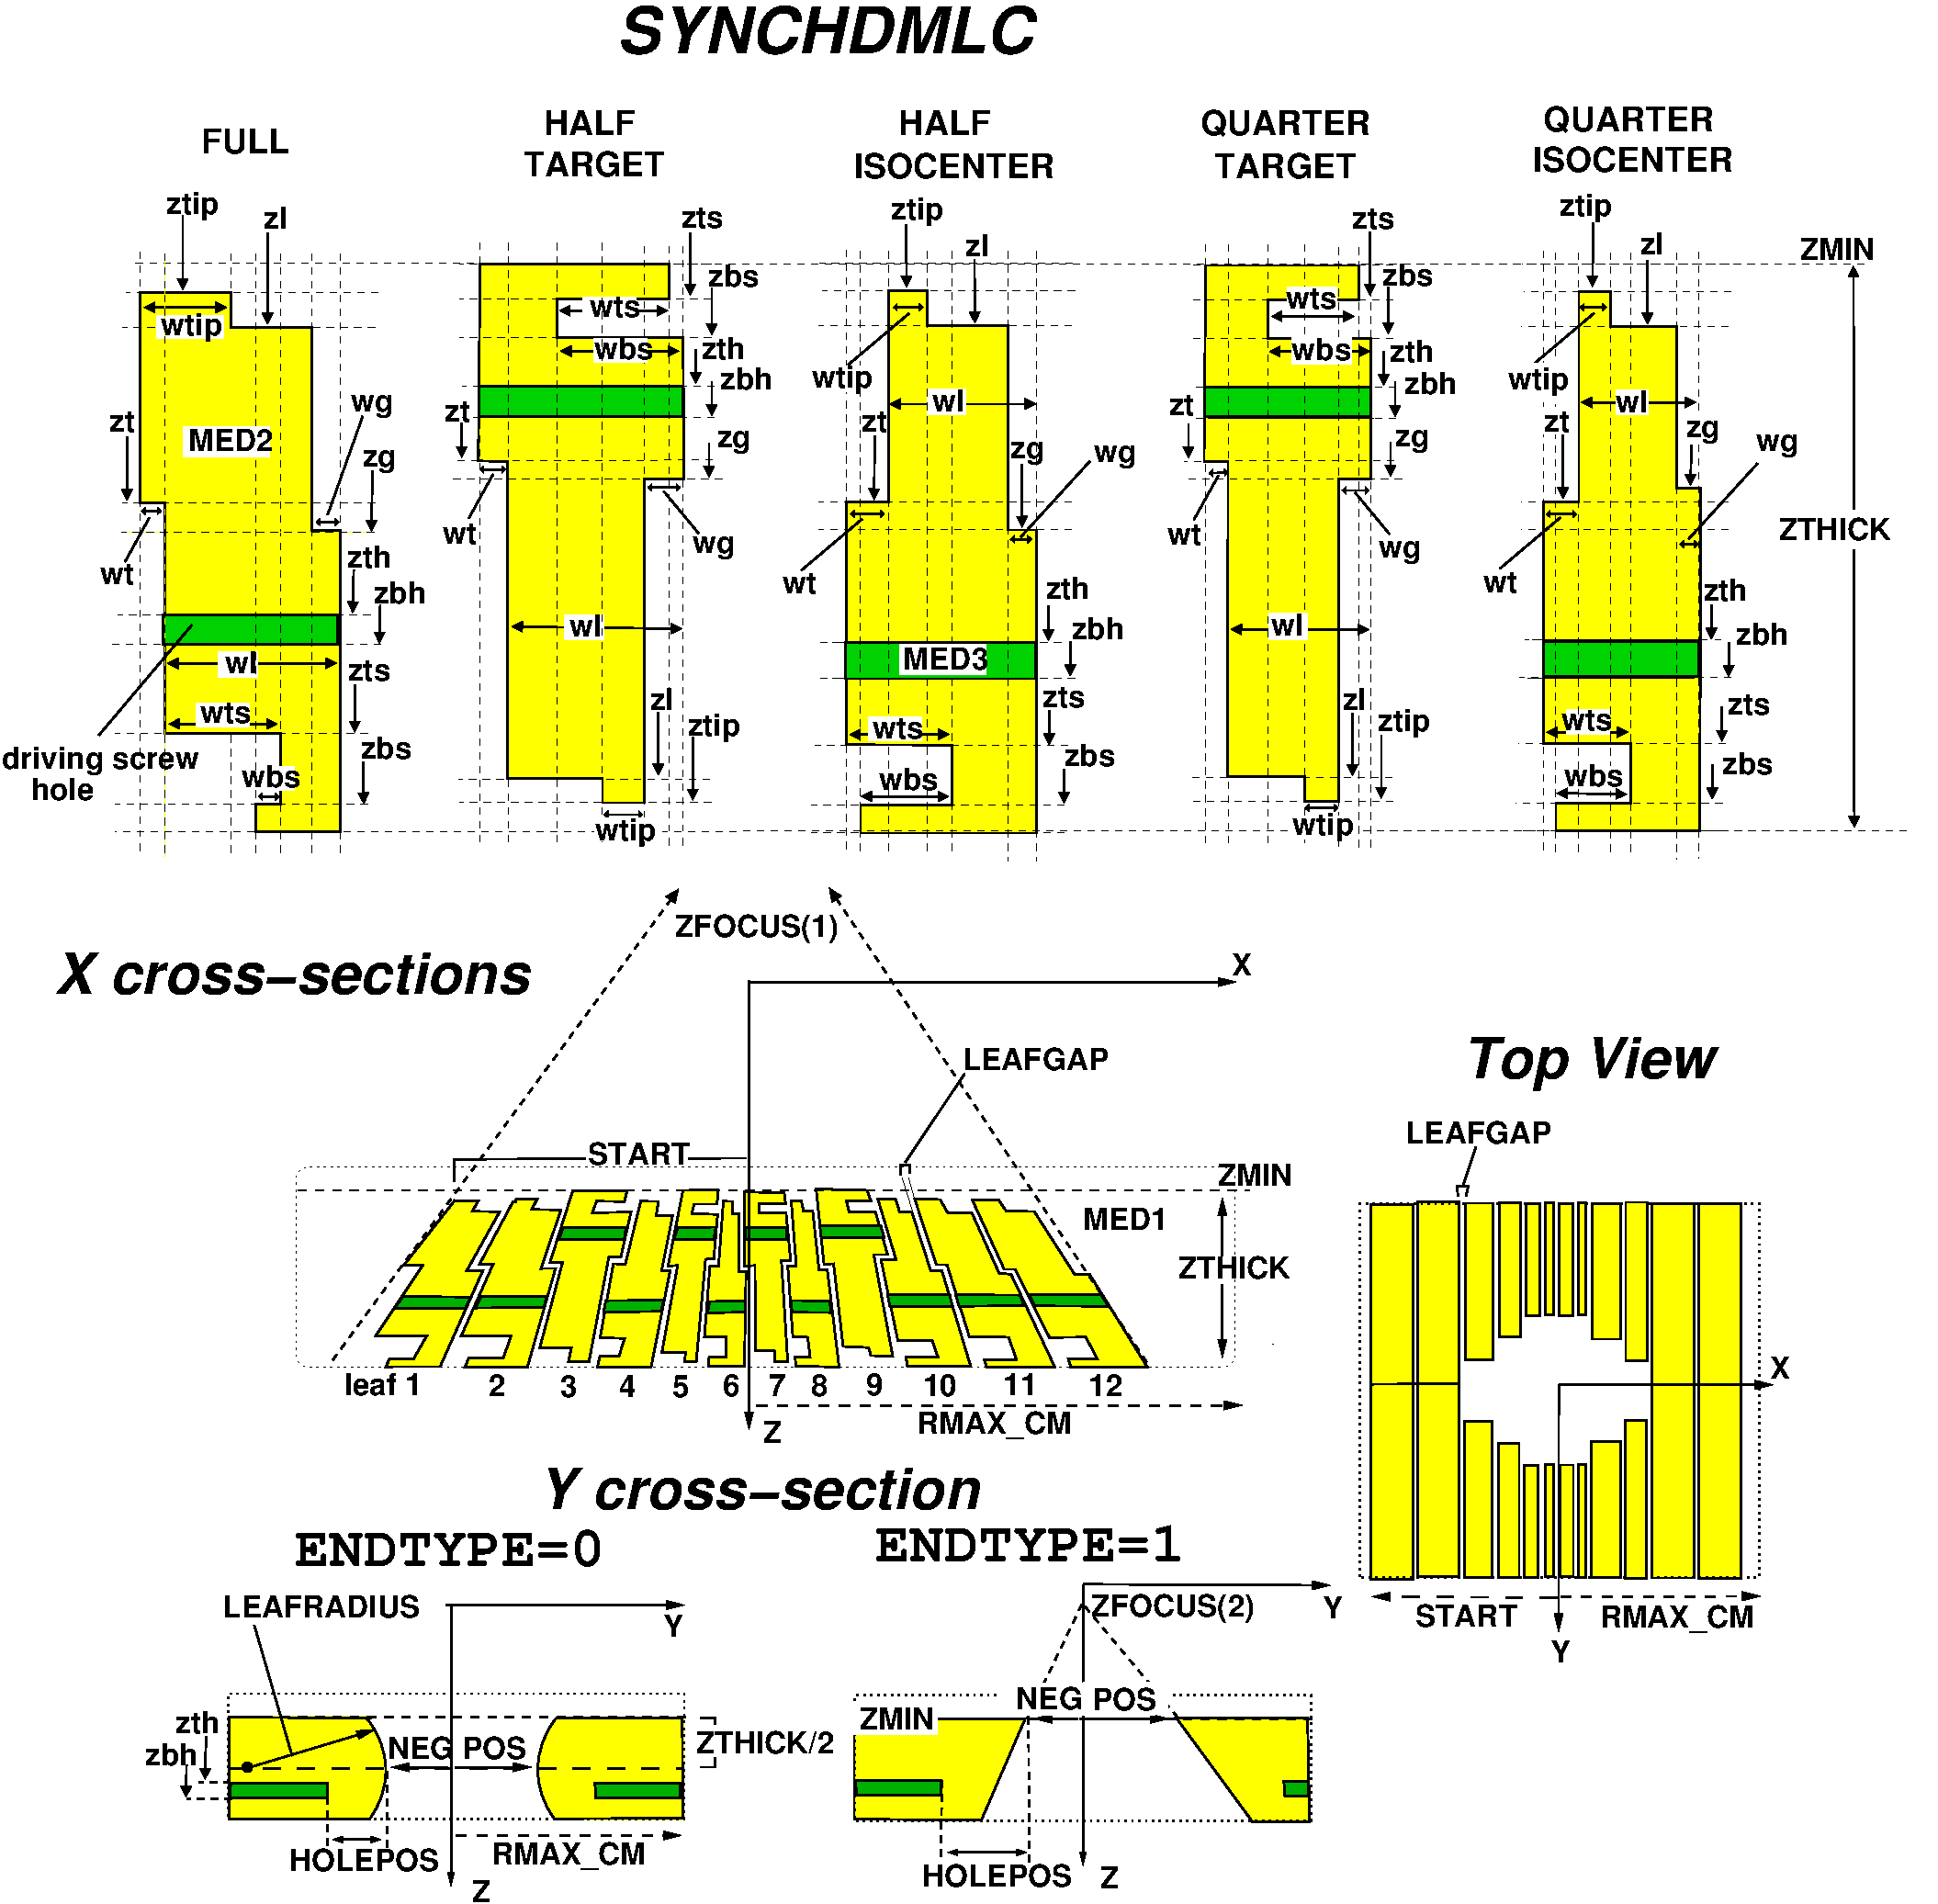
\includegraphics[width=21cm]{figures/synchdmlcd}
\end{latexonly}
\begin{htmlonly}
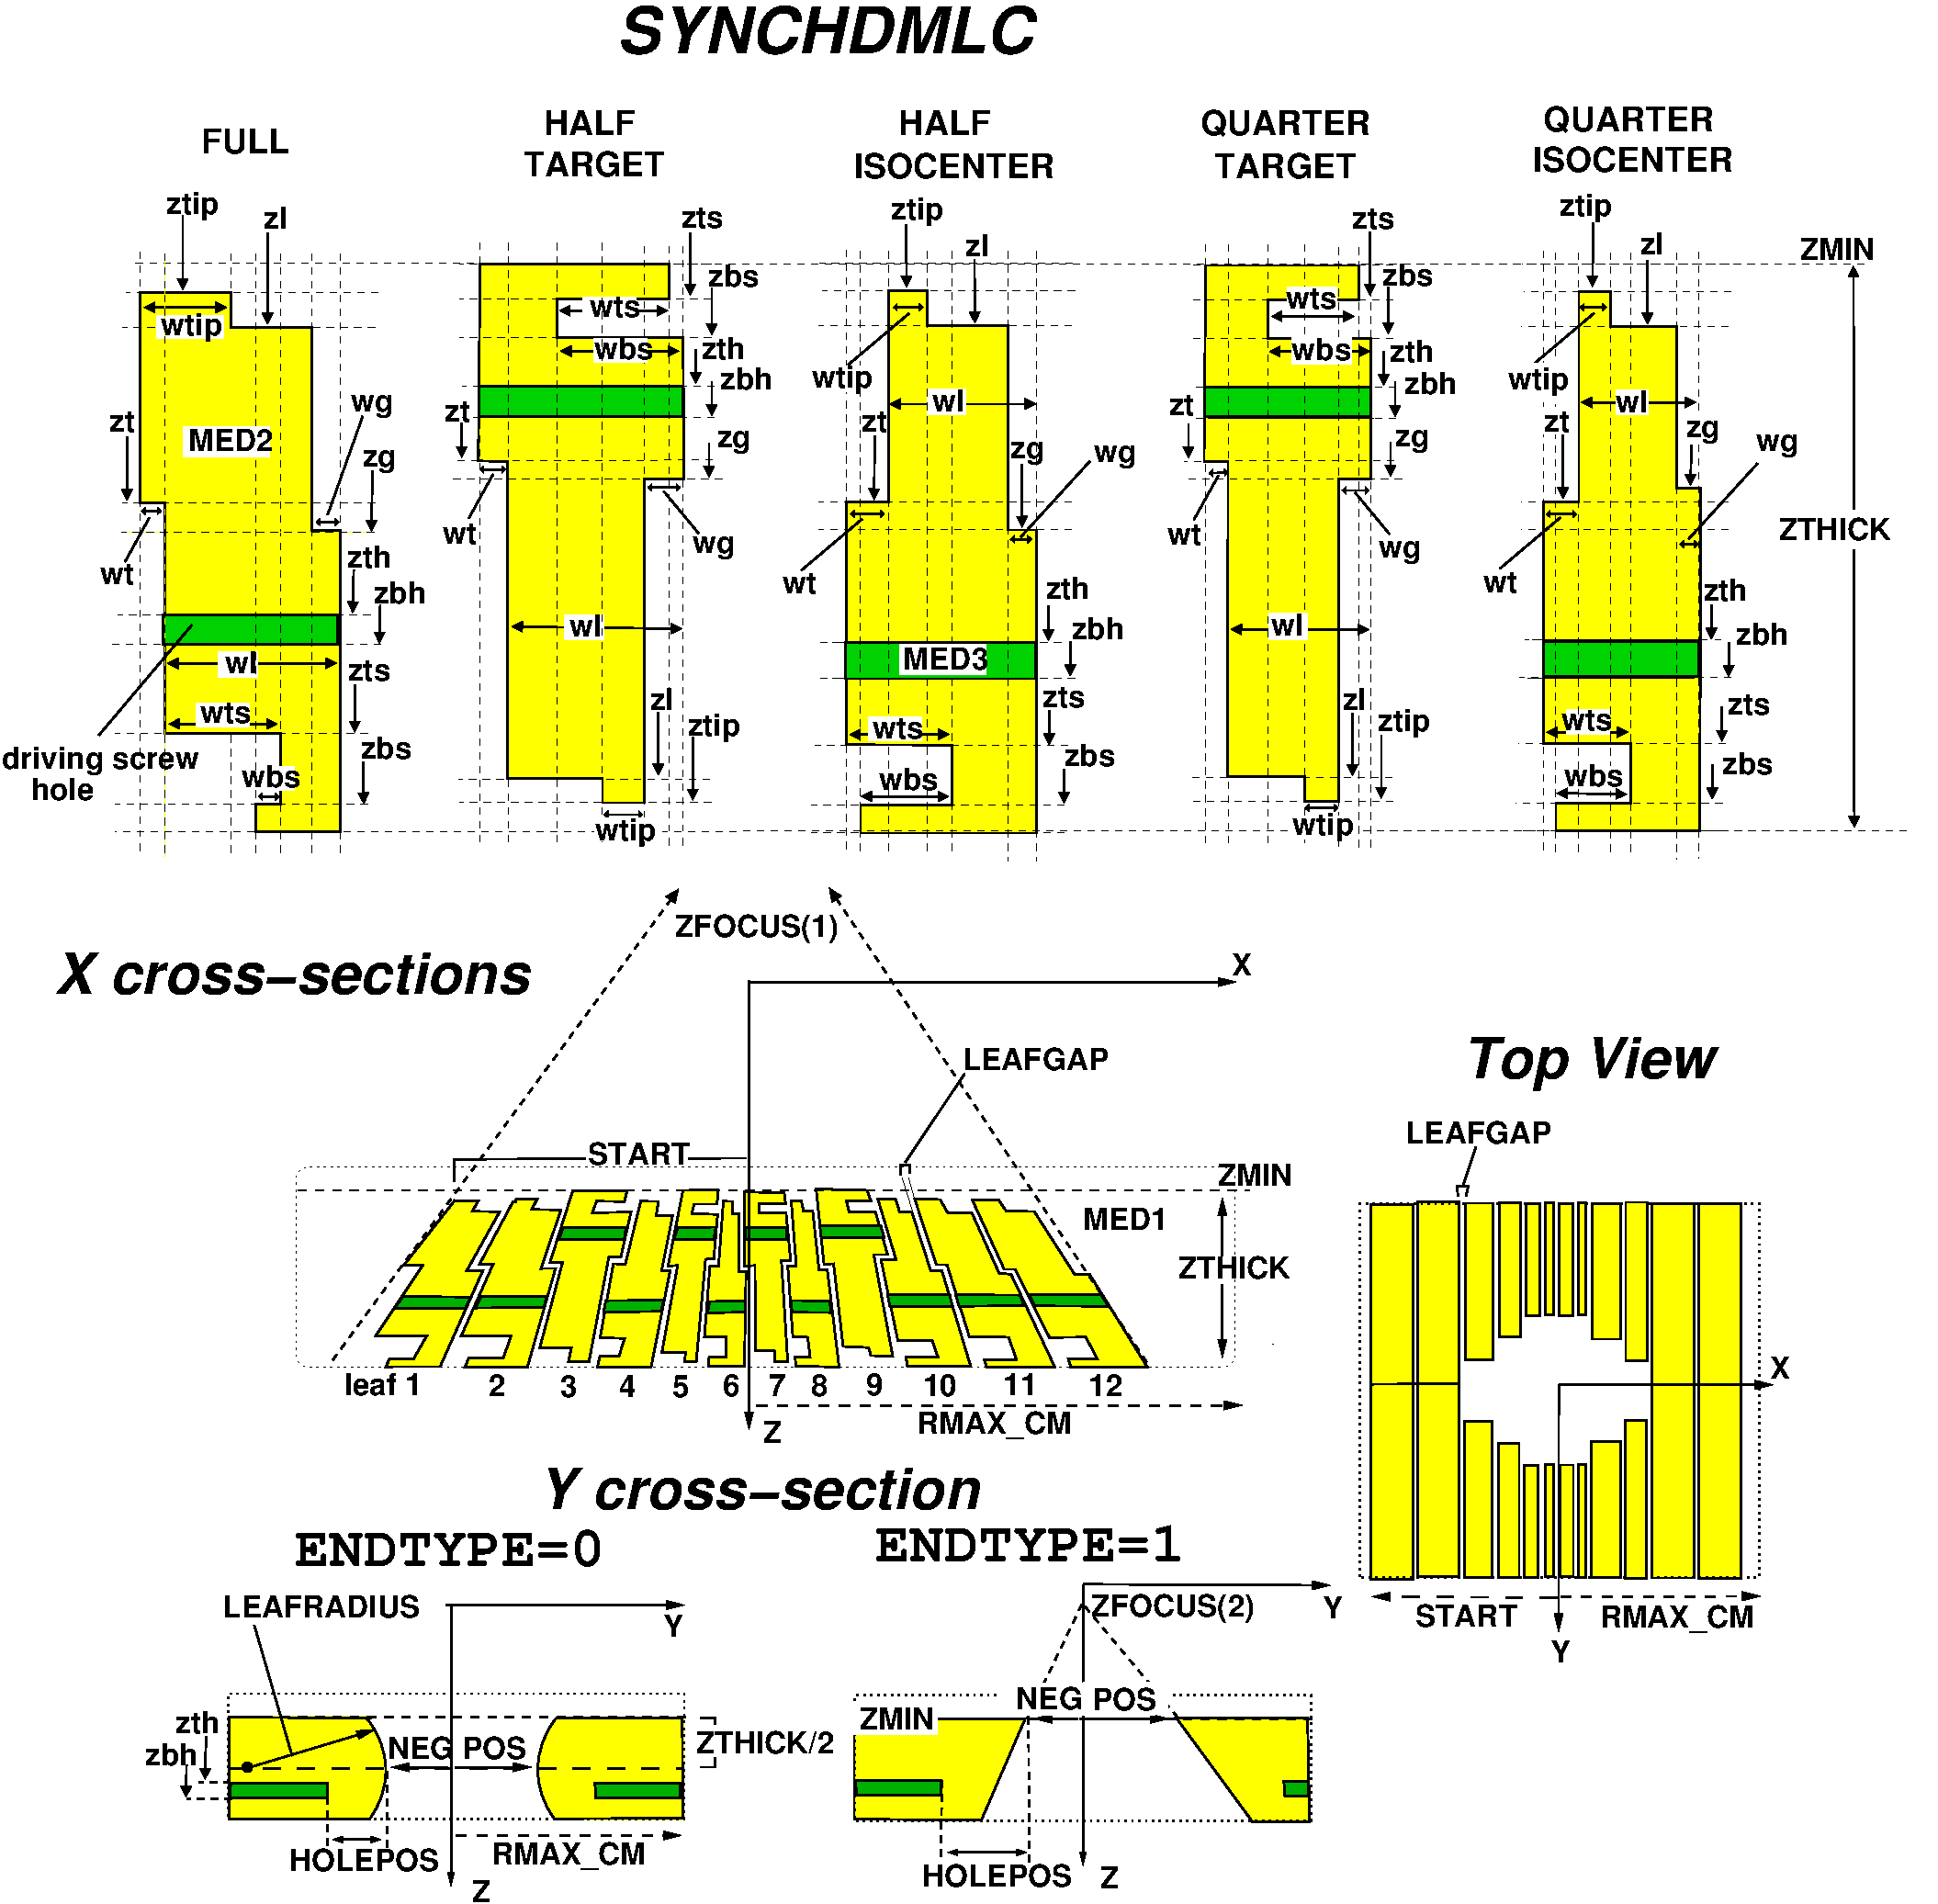
\includegraphics[width=13cm]{figures/synchdmlcd}
\end{htmlonly}
\end{center}
\vspace*{-1.0cm}
\caption[SYNCHDMLC CM geometry]
{Example SYNCHDMLC with 12 leaves opening in the Y
direction ({\tt ORIENT}=0). The X cross-sections of the five
leaf types show the dimensions that the
user must input (see Table~\ref{dynvmlc_tab} for label key).
QUARTER leaf cross-sections have similar Z-dimensions
to HALF leaf cross-sections but are thinner in X.
TARGET/ISOCENTER leaves must always occur in pairs.
In this illustration leaves 1, 2, 11, 12 are FULL; leaves 3, 4, 9, 10
are HALF TARGET/HALF ISOCENTER pairs; leaves 5--8 are QUARTER TARGET/QUARTER ISOCENTER
pairs.}
\label{synchdmlc_fig}
\end{figure}

\index{SYNCHDMLC!FULL leaves}\index{SYNCHDMLC!HALF TARGET leaves}
\index{SYNCHDMLC!HALF ISOCENTER leaves}\index{SYNCHDMLC!QUARTER TARGET leaves}
\index{SYNCHDMLC!QUARTER ISOCENTER leaves}
The labels on the cross-section dimensions in Figure~\ref{synchdmlc_fig}
have the same meanings as those used for DYNVMLC (See Section~\ref{dynvmlcsect} and
Table~\ref{dynvmlc_tab}).  In general, QUARTER leaves
are used closer to middle of the mlc, and, while their Z-dimensions are similar to those for their HALF counterparts, they
are significantly thinner in the X- ({\tt ORIENT}=0) or Y- ({\tt ORIENT}=1)
dimension.  HALF TARGET/HALF ISOCENTER leaves must occur in pairs, as must QUARTER TARGET/QUARTER ISOCENTER leaves.

\index{SYNCHDMLC!restrictions on leaf dimensions}
Similar to DYNVMLC, leaf cross-section dimensions must be defined so that the Z and X ({\tt ORIENT}=0) or Y ({\tt ORIENT}=1) grid lines
shown on the cross-sections at the top of Figure~\ref{synchdmlc_fig} do not change order.
The Z-positions of tongues and grooves must allow leaves to fit
together in the following
combinations: \\
FULL/FULL ({\tt zt}$_{FULL}$ $\leq$ {\tt zg}$_{FULL}$)\\
FULL/HALF TARGET ({\tt zg}$_{FULL}$ $\geq$ {\tt zt}$_{HALF~TARGET}$)\\
HALF TARGET/HALF ISOCENTER ({\tt zg}$_{HALF~TARGET}$ $\leq$ {\tt zt}$_{HALF~ISOCENTER}$)\\
HALF ISOCENTER/HALF TARGET ({\tt zg}$_{HALF~ISOCENTER}$ $\geq$ {\tt zt}$_{HALF~TARGET}$)\\
HALF ISOCENTER/QUARTER TARGET ({\tt zg}$_{HALF~ISOCENTER}$ $\geq$ {\tt zt}$_{QUARTER~TARGET}$)\\
QUARTER TARGET/QUARTER ISOCENTER ({\tt zg}$_{QUARTER~TARGET}$ $\leq$ {\tt zt}$_{QUARTER~ISOCENTER}$)\\
QUARTER ISOCENTER/QUARTER TARGET ({\tt zg}$_{QUARTER~ISOCENTER}$ $\geq$ {\tt zt}$_{QUARTER~TARGET}$)\\
QUARTER ISOCENTER/HALF TARGET ({\tt zg}$_{QUARTER~ISOCENTER}$ $\geq$ {\tt zt}$_{HALF~TARGET}$)\\
and HALF ISOCENTER/FULL (ie {\tt zg}$_{HALF~ISOCENTER}$ $\geq$ {\tt zt}$_{FULL}$).

As in DYNVMLC, rather than specifying the type of each leaf, the user is able to specify groups
of adjacent leaves all having the same type.  Since HALF TARGET/HALF ISOCENTER leaves and
QUARTER TARGET/QUARTER ISOCENTER leaves must always occur in pairs, there are really
only three types to choose from.  This also means there must be an even number of
HALF or QUARTER TARGET/ISOCENTER leaves.  Also note that, even though the user
must specify cross-sections for all leaf types, they need not use all types
in a given MLC simulation.  Thus, there may be no FULL leaves, HALF TARGET/ISOCENTER pairs,
or QUARTER TARGET/ISOCENTER pairs in the simulation.

Similar to DYNVMLC and SYNCVMLC, leaf ends can be straight, focused ({\tt ENDTYPE}=1) or cylindrical
({\tt ENDTYPE}=0).  For straight, focused ends, the user must specify the Z-position of the
focal point of the ends ({\tt ZFOCUS(2)}).  For cylindrical leaf ends, cylinders defining the leaf
ends all have their origin at Z={\tt ZMIN}+{\tt ZTHICK/2} ({\it i.e.} mid-way through the thickness
of the MLC) and user-specified radius, {\tt LEAFRADIUS}.  Positive and negative leaf opening coordinates, {\tt POS} and {\tt NEG}
are defined at Z={\tt ZMIN} for straight, focused leaf ends and at Z={\tt ZMIN}+{\tt ZTHICK/2} for cylindrical
leaf ends.

\index{SYNCHMDMLC!MODE}
If SYNCHDMLC is used in dynamic ({\tt MODE}=1) or step-and-shoot ({\tt MODE}=2) mode, then
leaf opening coordinates are read from a user-supplied file.  The format of the file
is identical to that used for DYNVMLC (and SYNCVMLC) and is given in
Section~\ref{dynvmlcsect} above.  Similar to the other synchronized CMs, the field indices,
{\tt INDEX(I)} are re-interpreted as {\tt muIndex(I)}, the fraction of monitor units delivered
up to and including field {\tt I}.  For each primary history, a random number {\tt MU\_RND}$\in[$0,1$]$ is
compared to the {\tt muIndex(I)} and is used to choose the field to use and,
in the case of dynamic mode, to calculate the opening coordinates using Equation (9).

The random number, {\tt MU\_RND}, is common for all synchronized CMs in the accelerator.  Thus, the
leaf settings for SYNCHDMLC can be synchronized with the settings of any other synchronized CMs.  In addition,
if a BEAM accelerator with SYNCHDMLC (and any other synchronized CMs) is compiled as a shared library for use
in DOSXYZnrc source 20 (synchronized phase space) or source 21 (synchronized BEAM treatment head), then
the value of {\tt MU\_RND} used in the BEAM simulation is passed to DOSXYZnrc.  This allows the motion of the source
plane in DOSXYZnrc to be synchronized with the opening coordinates in BEAMnrc.  Note the user must
define the coordination of source motion with CM opening coordinates.  See the DOSXYZnrc Users Manual\cite{Wa05}
for more details.

\index{SYNCHDMLC!IGNOREGAPS option}
Similar to DYNVMLC, SYNCHDMLC has an {\tt IGNOREGAPS} input parameter which, if set to 1, instructs the code to ignore
air gaps, driving screw holes and side boundaries of adjacent
leaves when determining the perpendicular
distance to the nearest region boundary for
charged particle range rejection.  For this option to be in effect, charged particles must be in the leaf medium and have:\\
particle Y ({\tt ORIENT}=0) or X ({\tt ORIENT}=1) $<$ minimum Y ({\tt ORIENT}=0) or X ({\tt ORIENT}=1) of all leaf openings
(excluding rounded or focused leaf end) or\\
particle Y ({\tt ORIENT}=0) or X ({\tt ORIENT}=1) $>$ maximum Y ({\tt ORIENT}=0) or X ({\tt ORIENT}=1) of all leaf openings (excluding leaf end)\\

An example of a file specifying dynamic leaf settings for SYNCHDMLC
is included with the distribution.  This file is {\tt \$OMEGA\_HOME/beamnrc/CMs/sample\_synchdmlc.sequence}.

A description of the input format for SYNCHDMLC is given below.

\begin{small}
\index{SYNCHDMLC!inputs}
\input{./inputformats/SYNCHDMLC.inp}
\end{small}
\index{input file!for SYNCHDMLC}


\clearpage

%\markboth{MESH Users Manual}{~~~~last edited 2004/11/19 20:21:18
%~~~~printed \today}
\vspace*{-2cm}
\renewcommand{\rightmark}{MESH CM}
\subsubsection{MESH}
\index{MESH}
The MESH CM models a single-layer wire mesh placed perpendicular
to the beam direction in the path of the beam.  Details are shown in
Figure~\ref{fig_MESHD} below.
\begin{figure}[H]
\begin{center}
\htmlimage{scale=2.0}
\leavevmode
\begin{latexonly}
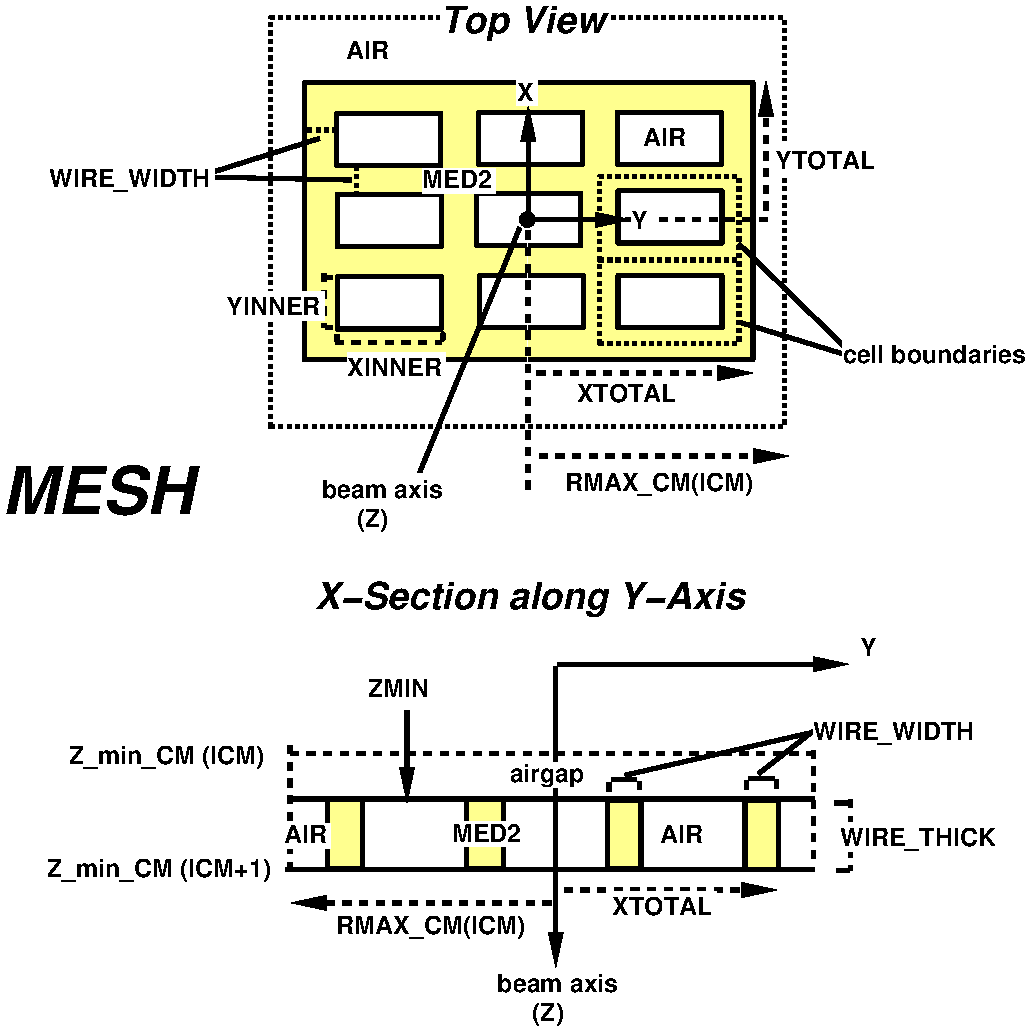
\includegraphics[height=14cm]{figures/meshd}
\end{latexonly}
\begin{htmlonly}
\includegraphics[height=13cm]{figures/meshd}
\end{htmlonly}
\end{center}
\vspace*{-0.5cm}
\caption[MESH CM geometry]
{A MESH component module.  The top view shows the identical rectangular
air ``holes'',
each with user-input dimensions {\tt XINNER} and {\tt YINNER}, separated
from each other and the edge of the mesh by wire of user-input width,
{\tt WIRE\_WIDTH}.  The outer boundaries of the mesh are defined by half-
widths {\tt XTOTAL} and {\tt YTOTAL} input by the user.  Note that
there is always one air hole centred on the beam axis.  The top view
also shows that a mesh ``cell'' is a single air hole plus half of
the wire surrounding it.  From a coding point of view, the mesh
is made up of adjacent cells which behave identically with respect to
particle transport.  Thus the code actually only models one cell (the
central one), and particles are translated from outer cells to their
equivalent positions in this cell before transport.  If the user-input
values of {\tt XTOTAL} and/or {\tt YTOTAL} happen to cut across cells,
the outer boundaries are automatically adjusted to accommodate these
cells.  The cross-section along the Y-axis shows the
Z position of the front of the mesh, {\tt ZMIN}, and the thickness of
the mesh, {\tt WIRE\_THICK}, both input by the user.  Note that it is
possible to have an air gap above the mesh.  For dose scoring and bit
setting purposes, the wire is considered a single region, and the air
in the holes and any air surrounding the mesh (excluding the air gap) are
considered another region.}
\label{fig_MESHD}
\end{figure}

\clearpage

The input format for MESH and an example input are given below.
\begin{small}
\index{MESH!inputs}
\input{./inputformats/MESH.inp}
\end{small}
\index{input file!for MESH}


\clearpage
%\markboth{MIRROR Users Manual}{~~~~last edited 2004/11/19 20:21:18
%~~~~printed \today}

\subsubsection{MIRROR}
\renewcommand{\rightmark}{MIRROR CM}
\index{MIRROR}

MIRROR is used for a mirror in the accelerator. It can have arbitrary
angle $<$ 85 degrees with respect to the Z axis (for angles between
85 and 90 degrees, approximate using SLABS).  The mirror portion itself can be
made up of an arbitrary
number
of layers having different thicknesses and media.  MIRROR has square symmetry.


\begin{figure}[htbp]
\begin{center}
\htmlimage{scale=2.0}
\leavevmode
\mbox{}\hspace{0cm}
\includegraphics[height=9cm]{figures/mirrord}
\caption[MIRROR CM geometry.]
{MIRROR example made up of 2 layers ({\tt N}=2).  The angle of the mirror with respect
to the Z-axis is determined by XFMIN and XBMIN, the positions of the
front face (layer 1) of the mirror, and {\tt ZTHICK} thickness of the
mirror in the Z-direction.  This angle must be $>$ 5 degrees.  The thickness of
layer i of the mirror is
given by {\tt DTHICK(i)}.  Note that layer i+1 of the mirror is flush with the
right-most face of layer i.  Thus, it is possible to specify a mirror
where some layers are out of the path of the beam.  It is even possible
to specify {\tt XFMIN} and {\tt XBMIN} so that the front face of the mirror (the
front face of layer 1) is out of the path of the beam; BEAMnrc checks for
this and gives a warning message.  The mirror extends to $+-${\tt RMAX\_CM} in
the Y-direction.  The media in front of and behind the mirror, {\tt MED4} and
{\tt MED3} in the figure, will usually be air but need not be.}
\label{fig_MIRRORD}
\end{center}
\end{figure}
\clearpage


The input format for MIRROR, and an example of input file are given as
follows.

\begin{small}
\index{MIRROR!inputs}
\input{./inputformats/MIRROR.inp}
\end{small}
\index{input file!for MIRROR}

%\markright{XTUBE: ~~~~beamnrc\_um.tex~~~~printed \today~~ last edited 2004/11/19 20:21:18
%}

%\markboth{XTUBE Users Manual}{~~~~last edited 2004/11/19 20:21:18
%~~~~printed \today}
\newpage
\subsubsection{XTUBE}
\renewcommand{\rightmark}{XTUBE CM}
\index{XTUBE}

A CM, which must be the first CM, for simulating an x-ray tube.  XTUBE is actually
similar in geometry to MIRROR.  However, unlike MIRROR, XTUBE is usually
the first CM in a beam model, and the source beam is usually incident on XTUBE
from the side.  The second CM may be any of the available  \verb+CMs+ with a
central opening serving as the exit
window of the x-ray tube.  The target of the xtube may
have an arbitrary number of layers, each with a different thickness and
medium.  XTUBE has square
symmetry.

\begin{figure}[htbp]
\begin{center}
\leavevmode
\mbox{}\hspace{0cm}
\includegraphics[height=9cm]{figures/xtubed}
\caption[XTUBE CM geometry.]
{XTUBE component module with 2 layers in the target ({\tt N}=2).
The angle of the target relative to the Z-axis is given by {\tt ANGLEI}.  The
thickness of a target layer i is given by {\tt DTHICK(i)}.  The target is
positioned so that the front of the target (layer 2 in the figure)
intersects with the beam at the central (Z) axis.  Target layers are
arranged with the front of layer i-1 flush with the back of layer i.
The target and target holder extend to $\pm$ {\tt RMAX\_CM} in the Y-direction.
MED3 in the figure above would usually be air or vacuum, but could be any
material.  MED4 specifies the material of the target holder.}
\label{fig_XTUBED}
\end{center}
\end{figure}
\clearpage

The input format for XTUBE and a sample input are given below.

\begin{small}
\index{XTUBE!inputs}
\input{./inputformats/XTUBE.inp}
\end{small}
\index{input file!for XTUBE}

\clearpage

\subsubsection{SIDETUBE}
\renewcommand{\rightmark}{SIDETUBE CM}
\index{SIDETUBE}

SIDETUBE is a CM for modelling concentric cylinders parallel to the
X-axis.  As one of 3 CMs in which a  radiating isotropic source ({\tt
ISOURC}=3) can be placed, it is designed for modelling any isotropic
source that is perpendicular to the beam/collimation.  The user can
specify the number, radii and media of the concentric cylinders, the X
positions of the cylinder ends, and the Z position of the axis of the
cylinders.  Note that all of the cylinders have the same end points, {\tt
XMIN} and {\tt XMAX}.  The user also specifies the medium surrounding the
outer cylinder and filling up the rest of the cube in which the cylinders
are contained.  SIDETUBE has square symmetry about the beam axis.

\begin{figure}[htbp]
\begin{center}
\leavevmode
\mbox{}\hspace{0cm}
\includegraphics[height=9cm]{figures/sidetubed}
\end{center}
\caption[SIDETUBE CM geometry.]
{SIDETUBE component module with 3 concentric cylinders ({\tt N}=3),
their common axis parallel to the X-axis and located at {\tt Z}={\tt ZCYL}.
The outer radii of the cylinders are given by {\tt r(1)}, {\tt r(2)},
{\tt r(3)}, and the
cylinders media are {\tt MED1}, {\tt MED2}, {\tt MED3}, respectively.  The
ends of the cylinders are specified by {\tt XMIN} and {\tt XMAX}.  {\tt MED4} is the user-specified medium surrounding the cylinders.  Note that all of the cylinders must fit
into the rectangular parallelepiped
defined by thickness, {\tt ZTHICK}, and half-width, {\tt RMAX\_CM}.  ZMIN,
the Z at which the cube containing the cylinders starts is not necessarily
equal to {\tt Z\_min\_CM(ICM)}, allowing an air gap at the top of this CM.}
\label{fig_SIDETUBED}
\end{figure}
\clearpage

The input format for SIDETUBE and a sample input are given below.

\begin{small}
\index{SIDETUBE!inputs}
\input{./inputformats/SIDETUBE.inp}
\end{small}
\index{input file!for SIDETUBE}

\clearpage

\subsubsection{ARCCHM}
\renewcommand{\rightmark}{ARCCHM CM}
\index{ARCCHM}

ARCCHM is a CM designed specifically for modelling an arc-shaped array of
chambers found in the prototype tomotherapy unit at the University of
Wisconsin.  However, it can be used
to model any arc-shaped structure in the path of the beam.  The arc is
always concave up and curves in the Y direction with the lowest point of the
arc (max. Z) always at Y=0.  The arc itself consists of a single layer of
chambers separated
by septa sandwiched between a chamber front face and chamber back face.  The
user specifies the Z position of the chamber front face at Y=0, {\tt ZSRC},
and the radius of the front face, {\tt ZRAD1}.
The angular extent of the arc
and it's total span in the Z direction are determined by other user-specified
parameters: the number of
chambers, {\tt NUMCHM} (which must be an even number), their width,
{\tt WIDTHCHM}, the width of the septa separating them, {\tt WIDTHSEP}, the
thickness of the chambers and septa, {\tt ARCTHICK}, and the thicknesses of
the chamber front and back, {\tt FRONTHCK} and {\tt BACKTHCK} respectively.
The chamber Y ends are automatically added and the chamber back face extended
so that they are flush with a plane at the minimum Z, {\tt ZMIN} (calculated,
not specified), of the
arc.  The user also specifies the minimum and maximum X limits of the
arc ({\tt XMIN1} and {\tt XMAX2}, respectively), the thickness of the
X ends of the chambers ({\tt WIDXWALL}) and the maximum Z of the CM
({\tt ZMAX}).
The user can specify the media in all regions of the CM with
the exception of the AIR above {\tt ZMIN}.  If the chambers all have
the same {\tt MED}, {\tt ECUT},
{\tt PCUT} and {\tt IREGION\_TO\_BIT} and the septa do as well, then
by setting {\tt IREPEAT}=1, the user only has to input these parameters once
for all chambers and once again for all septa.  In this case, if the {\tt DOSE\_ZONE}
input for the chambers is $>$0, then it is automatically incremented by
1 for each chamber, so that each chamber has its own dose zone.

This CM was originally coded by Marv Glass of the University of
Wisconsin.

\begin{figure}[htbp]
\htmlimage{scale=2.0}
\leavevmode
\begin{latexonly}
\hspace{-5cm}\includegraphics[height=14cm]{figures/arcchmd}
\end{latexonly}
\begin{htmlonly}
\includegraphics[height=12cm]{figures/arcchmd}
\end{htmlonly}
\caption[ARCCHM CM geometry.]
{ARCCHM component module with 4 chambers ({\tt NUMCHM}=4).  The number of
chambers must always be even so that they can be arrayed as shown in
the Y cross-section, with a
septum centred on the beam axis at Y=0.  The number of septa is always 1 less
than the number of chambers.  The user also specifies the Z position of the
front face of the chambers at Y=0, {\tt ZSRC}, the radius of the arc at the
front face, {\tt ZRAD1} ({\tt ZSRC}={\tt ZRAD1} for a perfectly isotropic
source), the arc-width of the chambers, {\tt WIDTHCHM}, and
septa, {\tt WIDTHSEP}, the thickness of the chambers/septa {\tt ARCTHCK},
the thickness of the front face, {\tt FRONTHCK}, and back face, {\tt BACKTHCK}
and the maximum Z of the CM, {\tt ZMAX}.  Other parameters such as the
angular extent of the arc, the minimum and maximum Y dimensions, {\tt YMIN1},
{\tt YMIN2}, {\tt YMAX1} and {\tt YMAX2}, and the minimum Z of the arc,
{\tt ZMIN} are calculated based on the user-specified parameters above.  As shown,
the chamber Y ends and back face are automatically extended so that they
are flush with {\tt ZMIN}.  Note that {\tt ZMAX} must be chosen
to accommodate the full Z range of the arc.  The cross-section in the X-direction
shows the user-specified minimum and maximum X of the arc ({\tt XMIN1} and
{\tt XMAX2} respectively) and width of the chamber X walls ({\tt WIDXWALL}).
The user can specify the medium in all regions except above {\tt ZMIN}.  If
all the chambers have the same {\tt MED}, {\tt ECUT}, etc, and the septa do
as well, then the number of inputs can be reduced by using the {\tt IREPEAT}
option.}
\label{fig_ARCCHMD}
\end{figure}
\clearpage

The input format for ARCCHM and a sample input are given below.

\begin{small}
\index{ARCCHM!inputs}
\input{./inputformats/ARCCHM.inp}
\end{small}
\index{input file!for ARCCHM}


%\markboth{BEAMnrc Users Manual}{~~~~~~last edited 2004/11/19 20:21:18
%~~~~printed \today}

\renewcommand{\rightmark}{Cross-section data-PEGS4}
\section{Cross-Section Data -- PEGS4}
\label{CSDP}
\index{PEGS4}
\index{cross section data}

Cross-section data for many commonly-used media are included in EGSnrc installation
in the files {\tt 521icru.pegs4dat} and {\tt 700icru.pegs4dat}, both
located in the {\tt \$HEN\_HOUSE/pegs4/data} directory.
The file {\tt 521icru.pegs4dat} consists of cross-section data
from a lower electron energy, {\tt AE}, of 0.521 MeV to an upper
electron energy, {\tt UE}, of 55 MeV, while {\tt 700icru.pegs4dat}
contains data from {\tt AE}=0.700 MeV to {\tt UE}=55 MeV.  In both
files the lower photon energy, {\tt AP}, is 0.01 MeV and
the upper photon energy, {\tt UP}, is 55 MeV.   These data are based on the
\index{AE}\index{AP}
density effect corrections in ICRU Report 37 \cite{ICRU37}.

If you wish to determine exactly what the composition of a given
material is, it is specified on the lines immediately following the
\verb+MEDIUM+ label in the {\tt .pegsdat} file.  For an up-to-date listing of
what materials are available in these files, do as follows
(only for Linux/Unix):\\
\verb+cd $HEN_HOUSE/pegs4/data+\\
\verb+grep MEDIUM 700icru.pegs4dat+
\\or\\
\verb+grep MEDIUM 521icru.pegs4dat+\\
To use these data you must specify the names {\bf exactly} as they
appear in the data file being used.

The NRC EGS user-code examin (found on {\tt \$HEN\_HOUSE/user\_codes/examin}) can
be used to tabulate or plot the various cross sections for each
material.

\index{creating PEGS4 cross section data}
\subsection{Creating additional cross section data}

Additional cross section data for BEAMnrc is created by the code PEGS4
(located in {\tt \$HEN\_HOUSE/pegs4}).
A complete description of the PEGS4 code is included in the EGSnrc
manual\cite{KR03}, and users wishing to create their own PEGS4 data
are referred to that manual.

\index{PEGS4!running}
Briefly, PEGS4 can be invoked on the command line by typing:
\begin{verbatim}
pegs4.exe -i inputfile [-d densityfile]
\end{verbatim}
\index{PEGS4!input file}
where {\tt inputfile} omits the {\tt .pegs4inp} extention and
{\tt densityfile} omits the {\tt .density} extension.  The {\tt .pegs4inp}
file specifies whether the the medium is an element ({\tt ELEM}),
compound ({\tt COMP}) or mixture ({\tt MIXT}); the composition of
the medium (by mass, {\tt RHOZ}, in the case of {\tt MIXT} and
number of atoms, {\tt PZ}, in the case of {\tt COMP}); the density ({\tt RHO};
whether Rayleigh cross-sections are to be included ({\tt IRAYL}=1);
the stopping powers calculated ({\tt IUNRST}=0 for restricted stopping
powers, {\tt IUNRST}=1 for unrestricted collision stopping powers, etc.);
and whether ICRU 37 density corrections are to be included
({\tt EPSTFL}=1).  The {\tt .pegs4inp} file also specifies the
values of {\tt AE}, {\tt AP}, {\tt UE} and {\tt UP} to use and the
name by which the medium will be referred in all input files using it.
There are other input options, but they are beyond the scope of this
manual.

\index{PEGS4!ICRU 37 density corrections}
If the user has selected to use ICRU 37 density corrections ({\tt EPSTFL}=1),
then they must include the {\tt -d densityfile} input when running
{\tt pegs4}.  Density correction files are found in the directory
{\tt \$HEN\_HOUSE/pegs4/density\_corrections}.  It is important to note that
if you are using a density correction file, the value of {\tt RHO} specified
in the {\tt .pegs4inp} file must match the material density in the
{\tt densityfile.density} file, which is the third value on the second
line of the file.

The EGSnrc distribution includes some sample input files in the
directory {\tt \$HEN\_HOUSE/pegs4/input}, and it is useful to use these
as references if creating your own {\tt .pegs4inp} file.

When running PEGS4 as described above PEGS4 data is automatically output
to either
{\tt \$HEN\_HOUSE/pegs4/data/inputfile.pegs4dat} or
{\tt \$EGS\_HOME/pegs4/data/inputfile.pegs4dat}, depending on what
directory it is being run from.

An much easier way to create PEGS4 data is to run PEGS4 from
the {\tt egs\_gui} (invoked simply by typing ``{\tt egs\_gui}'').  A screen
shot of the PEGS4 option in the {\tt egs\_gui} is shown in
Figure~\ref{fig_pegs4_screen}.  For more information on {\tt egs\_gui}
see the EGSnrcMP Manual\cite{Ka03}.

Note that {\tt egs\_gui} offers an option to append newly-created
PEGS4 data to an existing {\tt .pegs4dat} file.

\clearpage

\begin{figure}[ht]
   \htmlimage{scale=2.5}
   \leavevmode
   \begin{center}
%can be left out, but allows figures to be made
   \includegraphics[width=12cm]{figures/egs_gui_pegs4_screen}
    \end{center}
   \caption{Screen shot of the {\tt egs\_gui} set to run PEGS4 to create
an air data set. Filling in this form is much easier than creating an input
file and access to the density effect corrections is easy. The GUI
does not allow any value except {\tt IUNRST = 0}. For details, see
PIRS-877\cite{Ka03}. }
   \label{fig_pegs4_screen}
\end{figure}

\subsection{Choice of AE,AP}
\index{AE} \index{AP}
\label{AE}
\index{ECUT}  \index{PCUT}

The parameters  \verb+AP+ and  \verb+AE+ are the low-energy thresholds
for the production of secondary bremsstrahlung photons and knock-on
\index{bremsstrahlung!AP threshold}
electrons, respectively.  The parameters \verb+PCUT+ and \verb+ECUT+ are
required to be greater than or equal to \verb+AP+ and  \verb+AE+ (see
sections ~\ref{PCUTIN} and \ref{ECUTIN}).

Selection of \verb+AP+ is simple since one can afford to use a very low
value which ensures accurate photon transport.  We recommend using
\verb+AP+~=~0.010 MeV.  Note that in practice this means all
bremsstrahlung events are simulated as discrete events.

The choice of \verb+AE+
is more complex since there is some computing time associated
with lower values of \verb+AE+ and in some cases, lower values lead to
more accurate simulations.
The value of \verb+AE+ controls the statistical fluctuations in the
energy loss, can affect the electron step sizes and is a lower limit on
\verb+ECUT+. For a general discussion see, \eg\ \cite{Ro84,RB90}.

Although the choice of \verb+AE+ is complex in general,
it is fairly easy to give general rules for.
In practice, the value of \verb+AE+ has little effect on dose
calculations, except in the sense that  \verb+AE+ is the lower limit on
\verb+ECUT+.  Thus for dose calculations, one should select \verb+ECUT+
as discussed in section~\ref{ECUTIN} and then use  \verb+AE = ECUT+.
For calculations in which one is looking at electron spectra directly in
an electron beam, it is important to use a fairly low value of
\verb+AE+ in order to avoid well known artifacts\cite{Ro84,RB90}.
Figure~\ref{fig_AE_diff} gives an example of this artifact for the 9 MeV
beam from a Clinac2100C.  The spectrum calculated with AE=0.521 MeV is
clearly more realistic than that calculated with AE=0.700 MeV.
We find that \verb+AE+ = 0.521 MeV is adequate - but note, one can still
use \verb+ECUT+ much higher.

\vspace{5mm}
\begin{figure}[htbp]
\begin{center}
\leavevmode
\mbox{}\hspace{0cm}
\includegraphics[height=8.5cm]{figures/AE_diff}
\caption[Example of effects of AE=0.521 vs 0.700 on electron beam energy
spectrum.] {Example of the differences in electron spectra calculated
with AE=0.521 MeV and AE=0.700 MeV. The spectra are normalized to one
particle in the total spectrum. The specific example is for the 9
MeV beam from a Clinac2100C with a type III applicator.  The artifact
near the peak in the AE=0.700 MeV case is discussed in detail in
references~\cite{Ro84,RB90}.}
\label{fig_AE_diff}
\end{center}
\end{figure}

\subsection{Pegsless Mode}
\index{pegsless mode}
As of 2013, the user has the option of running BEAMnrc (and other EGSnrc user codes) in pegsless
mode, thus obviating the requirement for a-priori calculation of cross-section data and generation
of a {\tt .pegs4dat} file.  Photon interaction cross-sections have been calculated on-the-fly since
2006.  Thus, the migration to a fully pegsless implementation of EGSnrc required that
the calculation of electron cross-sections be similarly done on a simulation-by-simulation
basis.

To run in pegsless mode, the user must include parameters for calculating cross-sections, including
specifications for all media used in the simulation, in their {\tt .egsinp} file between the
delimiters, {\tt :start media definition:} and {\tt :stop media definition:}.  This is best illustrated
with an example input:

\begin{verbatim}
:start media definition:

AE=0.521
UE=50.511
AP=0.01
UP=50.

material data file=/home/username/HEN_HOUSE/pegs4/data/material.dat

:start H2O521ICRU:
  elements = H, O
  number of atoms = 2,1
  rho = 1.0
  bremsstrahlung correction = KM
:stop H2O521ICRU:

:start AIR521ICRU:
  elements = C,N,O,AR
  mass fractions = 1.24000E-04, 7.55200E-01, 2.31800E-01, 1.28300E-02
  rho = 1.2048E-03
  bremsstrahlung correction = NRC
  gas pressure = 1.0
:stop AIR521ICRU:

:start PMMA521ICRU:
  bremsstrahlung correction = NRC
  density correction file = /home/uname/EGSnrc/HEN_HOUSE/pegs4/density_corrections/
compounds/polymethylmethacrylate__lucite___perspex___plexiglas_.density
:stop PMMA521ICRU:

:stop media definition:
\end{verbatim}
where:
\begin{description}
\item {\tt AE,UE,AP,UP } are the kinetic energy limits for calculating photon ({\tt AP,UP}) and electron ({\tt AE,UE}) cross sections in
\index{pegsless mode!AE}\index{pegsless mode!UE}\index{pegsless mode!AP}\index{pegsless mode!UP}
MeV.  These energy limits are also mentioned in the context of the EGSnrc system in the section {\tt The COMMON Blocks}.
If {\tt AE} is
not specified it defaults to the highest value of {\tt ECUT} (electron transport cutoff energy--see Section {\tt Pre-HATCH Call Initialisation (Step 2)} in PIRS701) specified
in the simulation.  If
{\tt AP} is unspecified, then it defaults to the highest value of {\tt PCUT} (photon transport cutoff energy--see Section {\tt Pre-HATCH Call Initialisation (Step 2)} in PIRS701)
specified.  {\tt UE} and {\tt UP} default to 50.511 MeV and 50.0 MeV, respectively.

\index{pegsless mode!material data file}
\item {\tt material data file} is the name (including full directory path) of a file containing specifications for the media used
in the simulation.  Provided with the EGSnrc distribution is the material data file {\tt \$HEN\_HOUSE/pegs4/data/material.dat} which
contains specifications necessary to reproduce all of the cross-section data in {\tt 521icru.pegs4dat} and {\tt 700icru.pegs4dat}
(provided that the appropriate values of {\tt AE, UE, AP and UP} are specified--see above).  Note that the format for
media specifications in the material data file is similar to that used for specifying media directly in the
{\tt .egsinp} file, described immediately below.  In the case of the material data file, however, there is some redundancy in the specification to allow the
user to see the composition and density of the media.

\index{pegsless mode!defining media in .egsinp file}
\item the {\tt :start MEDNAME:} and {\tt :stop MEDNAME:} delimiters are used to specify medium, {\tt MEDNAME}, directly in the
{\tt .egsinp} file.  This method of specifying a medium is used if {\tt MEDNAME} is not included in the material data file or
if you wish to override some or all of the specifications for {\tt MEDNAME} in the material data file.
If no material data file is input, then all media in the simulation
must be specified in this way.  The inputs between these delimiters are described below.  Variables
in square brackets are the analogous PEGS4 variables described in the PEGS4 Manual (Section {\tt PEGS4 User Manual} in PIRS701) above.
\begin{description}
\index{pegsless mode!elements}
\item {\tt elements} specifies the elements comprising the medium.  Elements are specified using chemical symbols separated by
commas.  Case is unimportant.
\index{pegsless mode!no. of atoms}
\index{pegsless mode!mass fractions}
\item {\tt number of atoms} $[${\tt PZ}$]$ or {\tt mass fractions} $[${\tt RHOZ}$]$.  For each of the {\tt elements}, specify either the number of atoms in a molecule of the medium ({\it i.e.} stoichiometric coefficients), if the
medium is a compound, or the mass fractions of the elements in the medium,
if the medium is a mixture.
Values are separated by commas and are input in the same order as their corresponding elements.  In the example above,
the composition of {\tt H2O521ICRU} is
defined using the number of atoms of each element, while that of {\tt AIR521ICRU} is defined using the mass fraction of each element.  Note that this input
is omitted if the medium is an element.
\index{pegsless mode!rho}
\index{pegsless mode!bulk density}
\item {\tt rho} specifies the bulk density of the medium in g/cm$^3$.
\index{pegsless mode!stopping power type}
\index{pegsless mode!bremsstrahlung correction}
\index{pegsless mode!IAPRIM}
\item {\tt bremsstrahlung correction} $[${\tt IAPRIM}$]$ specifies the
correction to apply to calculated bremsstrahlung cross-sections.
Options are:
\begin{itemize}
\item {\tt KM} $[$IAPRIM=0$]$ (the default): Apply Koch and Motz\cite{KM59} empirical corrections.
\item {\tt NRC} $[$IAPRIM=1$]$: Apply NRC corrections based on NIST/ICRU\cite{Ro89a}.  These corrections are read from the file
{\tt \$HEN\_HOUSE/pegs4/aprime.data}.
\item {\tt None} $[$IAPRIM=2$]$: No corrections applied.
\end{itemize}
\index{pegsless mode!density correction file}
\index{pegsless mode!EPSTFL}
\item {\tt density correction file} $[${\tt EPSTFL}$]$ is the name of a file containing density effects which, when applied to calculated collision
stopping powers, results in agreement with collision stopping powers published in ICRU37\cite{ICRU37}.  In general, density correction files are specified including their full directory path and {\tt .density} file extension.  However,
the file can be specified by its prefix only if it
exists in, in order of search priority:
\begin{enumerate}
\item {\tt \$EGS\_HOME/pegs4/density\_corrections}
\item {\tt \$EGS\_HOME/pegs4/density\_corrections/elements}
\item {\tt \$EGS\_HOME/pegs4/density\_corrections/compounds}
\item {\tt \$EGS\_HOME/pegs4/density}
\item {\tt \$HEN\_HOUSE/pegs4/density\_corrections/elements}
\item {\tt \$HEN\_HOUSE/pegs4/density\_corrections/compounds}
\end{enumerate}
Note that the density correction files for many elements, compounds
and mixtures are supplied with
the distribution.  Density correction files have a header portion from which the composition and bulk density of the medium are read.  These values override
any user inputs for {\tt elements=}, {\tt number of atoms=} or {\tt mass fractions=}, and {\tt rho=}.  Thus, as in the case of
{\tt PMMA521ICRU} in the example above, it is possible to specify the composition
of a medium simply by specifying a density correction file.
\index{pegsless mode!gas pressure}
\index{pegsless mode!GASP}
\item {\tt gas pressure} $[${\tt GASP}$]$ is the pressure of the medium in atm
if the medium is a gas.  This input is only relevant (and necessary
for a gas) if
a density correction file is not used, in which case {\tt gas pressure} is used to modify the calculated density effect parameters.
{\tt gas pressure} defaults to 0 ({\em i.e.} the medium is not a gas).
\end{description}
\end{description}

Inputs specifying media are case insensitive with the exception of the medium name ({\it e.g.} {\tt H2O521ICRU} is
different than {\tt h2o521ICRU}).

Note that, along with the medium name, the medium composition, specified by {\tt elements} and {\tt number of atoms} or {\tt mass fractions}, and its bulk density, specified by {\tt rho}, are
sufficient to calculate cross-sections.  Thus, it is possible to completely define a medium
using only these three inputs, with all other parameters reverting to their default values or remaining blank.
Alternatively, since composition and bulk density can be read from the header of the density correction file, it is also possible to define a medium
simply by specifying the name of the relevant density correction file.

The BEAM GUI allows you to define and modify the media definition section of the {\tt .egsinp} file through the
``Define Media'' button in the ``Main Inputs'' window.  This button is enabled when you go into ``Change PEGS4 file''
under the ``File'' menu and opt to ``Go PEGSless''.

\index{pegsless mode!running code}
{\bf Running in Pegsless Mode}

BEAMnrc can be run interactively in pegless mode using the command line input:
\begin{verbatim}
BEAM_myaccel -i inputfile
\end{verbatim}
where {\tt inputfile} is the name of the BEAM inputfile (with no
{\tt .egsinp} extension).

Pegsless batch runs use the command line syntax:
\begin{verbatim}
exb BEAM_myaccel inputfile pegsless [short|medium|long] [batch=batch_system] [p=N]
\end{verbatim}
This is identical to the syntax of a run with pegs data (see Section~\ref{batchsect} above) but
with the word {\tt pegsless} in place of the name of the pegs data file.

\index{.mederr file}
When running in pegsless mode, BEAMnrc outputs a file, {\tt inputfile.mederr}, which, for each medium used
in the simulation, indicates where each specifying parameter has been read ({\it i.e.} from a material data
file or directly from the {\tt .egsinp} file).  The file also includes warnings when {\tt AE}, {\tt UE},
{\tt AP} or {\tt UP} have not been specified and have been set to their default values and when a material
data file has not been specified.  For parallel runs in pegsless mode (parameter {\tt p} $>$ 1 in the batch
command syntax above), the {\tt .mederr} file is only output by the first job.

The actual values of the media specifications (including defaults) used to calculate cross-sections are
output in the listing file, {\tt inputfile.egslst}, and to the screen for interactive runs or in the
log file, {\tt inputfile.egslog}, for batch runs.

\section{Distribution and Installation}
\renewcommand{\rightmark}{Distribution and Installation}
\label{installbeam}
\index{distribution}
\index{installation}

% Installation of the OMEGA/BEAM codes requires you to have already
% installed and configured EGSnrcMP on your system.  A brief description of
% the installation/configuration of
% EGSnrcMP will be given here, but for more detail you are
% urged to refer to the EGSnrcMP Users Manual\cite{Ka03}.

For up-to-date installation instructions, see the online documentation
available on the github page:
\htmladdnormallink{{\tt https://github.com/nrc-cnrc/EGSnrc/wiki/Installation-overview}}{https://github.com/nrc-cnrc/EGSnrc/wiki/Installation-overview}

In order to install and run EGSnrcMP and OMEGA/BEAM, your system must have:
\index{system requirements}
\begin{enumerate}
\index{Fortran compiler}
\item A working Fortran compiler.  If you do not have one on
your system, GNU provides a suite of compilers that can be downloaded
for free at \htmladdnormallink{{\tt http://www.gnu.org}}{http://www.gnu.org}
\index{make utility}
\item A working {\tt make} utility.  Most systems have this built in, although
there is one available at the GNU site as well.
\index{C/C++ compiler}
\item A working C or C++ compiler.  This is a requirement on Unix/Linux
systems if you want to take advantage of
the built-in parallel processing capability of BEAMnrc and DOSXYZnrc
(and other EGSnrc user codes) and is of no use if you do not
have a batch submission capability.  It is also required on Unix/Linux
systems (but not on Windows) if you want to use a BEAM simulation as a
source with DOSXYZnrc or with any other EGSnrc user code.
The compiler is available at the GNU site.
\index{C++ compiler}
\item A working C++ compiler.  This is required if you want to be
able to read/write IAEA-format phase space files.
\index{Tcl/Tk}
\index{Tcl/Tk!how to get it}
\item Tcl/Tk.  This is necessary for running the BEAMnrc, DOSXYZnrc and
BEAMDP GUIs.  It can be downloaded from
\htmladdnormallink{{\tt http://www.activestate.com/activetcl/downloads}}{http://www.activestate.com/activetcl/downloads}.  See the GUI User's Manual\cite{Tr04} for
more information.  Note that most Linux distributions already include
Tcl/Tk.
\index{Qt}
\index{Qt!how to get it}
\item The Qt4 development tools. This is necessary for
compiling the GUIs for the EGSnrcMP user codes and is, thus,
not strictly necessary for the OMEGA/BEAM codes or if you can use the
pre-compiled versions provided online. Pre-compiled versions of
the Qt GUIs are available on the EGSnrc release page.
Note that many current Linux distributions
include Qt, since the popular Desktop Environment KDE is based on Qt.

\index{xmgrace}
\item The Grace plotting package ({\tt xmgrace} command) which is available at\\
\htmladdnormallink{{\tt http://plasma-gate.weizmann.ac.il/Grace}}
 {http://plasma-gate.weizmann.ac.il/Grace}. This is distributed with many
Linux distributions and there is a Windows version called QtGrace.
\end{enumerate}


%%%%%%%%%%% Have to rewrite installation instructions for github distribution

% Note that some of these system requirements are included as part of
% the EGSnrcMP distribution (depending upon which method you choose to
% install EGSnrcMP).  More details about this will be given below.

% \subsection{Installing EGSnrcMP}
%
% \index{EGSnrcMP!installation}
% \index{EGSnrcMP!distribution site}
% The EGSnrcMP distribution is available online.  Download the
% version appropriate for your system.  There are several
% different methods for installing the system.  The easiest of these
% \index{EGSnrcMP!installation wizard}
% is ``Method 1'', the self-extracting installation wizard.  This includes
% compressed versions of all codes required for a complete EGSnrcMP
% distribution which are automatically uncompressed at installation time.
% In the case of Windows, the self
% extracting download also includes GNU Fortran, C and C++ compilers
% and the GNU {\tt make} utility.
%
% \index{EGSnrcMP!installation wizard}
% ``Method 2'' for installing EGSnrcMP involves downloading the
% installation wizard and the required, compressed codes separately.  In
% addition to the installation wizard itself, the
% required downloads to install a complete EGSnrcMP system are:
% \begin{description}
% \index{EGSnrcMP!.egszip files}
% \item[{\tt V4\_EGSnrc.egszip}] The EGSnrcMP system.
% \item[{\tt V4\_spinms.egszip}] Spin and multiple-scattering data.
% \item[{\tt V4\_user\_codes.egszip}] The EGSnrcMP user codes.  Not
% necessary if you are only planning to run the OMEGA/BEAM codes.
% \item[{\tt V4\_manuals.egszip}] EGSnrcMP documentation.
% \end{description}
% Additional downloads for Windows are:
% \begin{description}
% \index{GNU compilers for Windows}
% \item [{\tt V4\_MinGW.egszip}] GNU Fortran, C, C++ compilers and
% {\tt make} utility.  Only required if you do not have working
% versions of these on your system.
% \item [{\tt V4\_winstuff.egszip}] GUIs for EGSnrcMP user codes and other
% Windows-specific codes.
% \end{description}
% \index{EGSnrcMP!user code GUIs}
% For Unix/Linux, if you are planning to use the GUIs for the EGSnrcMP
% user codes (not necessary if you are only going to run the OMEGA/BEAM
% codes), then you should also download the GUI codes,
% {\tt V4\_EGSgui.egszip}.  These downloads and their functions are made
% clear on the distribution website.  If you have only downloaded a subset
% of the above {\tt .egszip} files ({\em e.g.} the minimum required
% for eventually installing/running the OMEGA/BEAM codes) then you should
% instruct the GUI to only uncompress those archives that you have
% downloaded.
% Rather than physically dowloading
% the {\tt .egszip} files yourself, you can also instruct the GUI
% to automatically download the archives (any subset of them or
% all of them) from
% the distribution website before installation.   Note that ``Method 1'' and
% ``Method 2'' for
% EGSnrc installation are
% not available for the Mac OSX.
%
% The third method, ``Method 3'', of installing EGSnrcMP is for
% \index{EGSnrcMP!installation script}
% Unix/Linux systems and Mac OSX systems and uses the installation script
% {\tt install\_egs}.  In addition to the script, you must also download
% \index{EGSnrcMP!.tar files}
% the {\tt tar} files (which may be in compressed format)
% \begin{description}
% \item {\tt V4\_EGSnrc.tar[ |.gz|.bz2] }
% \item {\tt V4\_EGSgui.tar[ |.gz|.bz2] }
% \item {\tt V4\_manuals.tar[ |.gz|.bz2] }
% \item {\tt V4\_user\_codes.tar[ |.gz|.bz2] }
% \item {\tt V4\_spinms.tar[ |.gz|.bz2] }
% \end{description}
% where the base names of the files are the same as for the {\tt .egszip}
% files described above.  These files must all be in the same
% directory before running the {\tt install\_egs} script.  This method
% of installation may be necessary if your Linux/Unix system cannot
% run the installation wizard and is currently the only way of
% installing EGSnrcMP on Mac OSX.  Note that when you use this
% method of installation, you must
% run the script {\tt \$HEN\_HOUSE/scripts/finalize\_egs\_foruser}
% at the end ({\tt install\_egs} gives you an option to do this
% automatically) in order to define/create your
% {\tt \$EGS\_HOME} area (see next paragraph).
% \index{finalize\_egs\_foruser}
%
% During installation of EGSnrcMP, you will be asked to define
% \index{\$HEN\_HOUSE}
% \index{\$EGS\_HOME}
% the location of {\tt \$HEN\_HOUSE}, the repository for
% all EGSnrcMP and OMEGA/BEAM codes (see Figure~\ref{fig_hen_house},
% page~\pageref{fig_hen_house}),
% and your {\tt \$EGS\_HOME} area, where
% each compiled user code (including accelerators modeled with
% BEAMnrc) has a subdirectory (see Figure~\ref{fig_users_area}).  You will
% also be asked to define the Fortran compiler that
% you want to use (defaults are suggested if found on your system).
% \index{installation!C compiler}.
% On Unix/Linux/Mac OSX systems, if you wish to use functionality that requires a C compiler such
% as the built-in parallel processing functionality
% (see Section~\ref{parallelcalc}) or BEAMnrc shared
% library sources (see Section~\ref{sharedlibsect}),
% then you must also supply the name of a working
% C compiler at this point (default C compilers are suggested
% if found on your system).  On Windows systems, the parallel processing
% is unavailable (no batch queuing system) and a precompiled object file required
% for BEAM shared library sources is provided during installation, so the
% reason to specify a C compiler here is to make use of the C interfaces which
% allow EGSnrc user codes to be written in C (see the EGSnrcMP Manual\cite{Ka04b}
% for more details).
% You will be asked to give a name to your
% machine configuration
% and supply a prefix for the configuration file, \ie, the {\tt .conf} file.
% The name you give for your configuration will determine the names of the
% subdirectories off {\tt \$HEN\_HOUSE/lib}
% \index{.conf file}
% \index{configuration}
% {\tt \$HEN\_HOUSE/bin} and {\tt \$EGS\_HOME/bin}.  See
% section~\ref{dirstructsect}, page~\pageref{dirstructsect}, for more
% information about the directory structure of the {\tt \$HEN\_HOUSE}
% and section~\ref{makefilesect}, page~\pageref{makefilesect} for more
% information about the {\tt .conf} file.  We recommend that the prefix
% of the {\tt .conf} file be the same as the configuration name to avoid
% confusion.  Finally, you will be given the option
% to input the name of a working
% \index{installation!C++ compiler}
% C++ compiler (default C++ compilers are suggested if found
% on your system).  This is required
% to compile the library necessary for
% reading/writing IAEA-format phase space data
% (see Section~\ref{iaeasect}) on all systems and to allow compilation of the
% EGSnrc C++ class library, egspp (see the egspp Manual\cite{Ka05a} for more
% details).
%
% Note that, on Unix/Linux/Mac OSX machines, if you supply a working C compiler
% during EGSnrcMP installation
% and the C routines for built-in parallel processing and/or BEAM shared
% library sources are compiled successfully, then the installation automatically
% sets up your {\tt config.conf} to enable these functions.  Similarly,
% on all systems,
% if you supply a working C++ compiler during installation and the library
% of IAEA phase space handling routines is compiled successfully, the
% installation automatically configures {\tt config.conf} so that user
% codes link this library ({\tt \$HEN\_HOUSE/iaea\_phsp/iaea\_phsp.a})
% during compilation and can read/write IAEA-format phase space data.
%
% \index{\$HEN\_HOUSE}
% \index{\$EGS\_HOME}
% \index{\$EGS\_CONFIG}
% When installing on Windows, you will be given the option
% to automatically set the environment variables {\tt HEN\_HOUSE},
% {\tt EGS\_HOME} and {\tt EGS\_CONFIG} (which is set to\\
% {\tt \$HEN\_HOUSE/specs/config.conf}, where
% {\tt config} is the prefix you have chosen for
% the {\tt .conf} file).  It is recommended that
% you do this to avoid having to add them manually.  When installing
% on Unix/Linux/Mac OSX, on the other hand, you do not have the option to set
% these variables automatically.  Instead, you will be directed to
% add the statements:
% \index{.cshrc}
% \index{.bashrc}
% \index{egsnrc\_cshrc\_additions}
% \index{egsnrc\_bashrc\_additions}
% \begin{verbatim}
% setenv EGS_HOME /full directory path to your EGS_HOME/
% (or export EGS_HOME=/full directory path to your EGS_HOME/)
% setenv EGS_CONFIG /full_path_to_your_HEN_HOUSE/specs/config.conf
% (or export EGS_CONFIG=/full_path_to_your_HEN_HOUSE/specs/config.conf)
% source /full_path_to_your_HEN_HOUSE/scripts/egsnrc_cshrc_additions
% (or . /full_path_to_your_HEN_HOUSE/scripts/egsnrc_bashrc_additions)
% \end{verbatim}
% to the {\tt .cshrc} (or {\tt .bashrc}) file in your {\tt \$HOME} area.  These
% directions are
% \index{\$HEN\_HOUSE}
% \index{README\_UNIX}
% reiterated in the file {\tt \$HEN\_HOUSE/README\_UNIX}.  Note that
% the {\tt egsnrc\_cshrc\_additions} (or {\tt egsnrc\_bashrc\_additions}) script
% defines {\tt \$HEN\_HOUSE}.  Once you have
% added these statements, you will then have to {\tt source} your
% {\tt .cshrc} (or {\tt .bashrc}) file, or else open a new window, to run
% EGSnrcMP.
%
% If you are using a batch queuing system (Unix/Linux only) then the file \\
% {\tt \$HEN\_HOUSE/scripts/batch\_options.YourSystemName} must exist
% (the distribution includes files for {\tt at}, {\tt pbs}, {\tt keg} and
% {\tt nqs} but these may require modifications for your system)
% and you also must include:\\
% {\tt setenv EGS\_BATCH YourSystemName}\\
% in your {\tt .cshrc} file or equivalent in your {\tt .bashrc} file.
%
% If you wish to use a second compiler or operating system, you can either
% run the installation wizard (self-extracting or stand-alone) and
% select the ``Configure existing EGSnrc'' option or, if on a Unix/Linux/Mac OSX
% system, you can run the
% script\\
%  {\tt \$HEN\_HOUSE/scripts/configure} from the {\tt
% \$HEN\_HOUSE/scripts} directory.  Alternatively, this task
% can be done from the {\tt egs\_gui}
% interactive GUI for general EGSnrc user codes\cite{Ma03}.
% Note that you must have write permissions
% on {\tt \$HEN\_HOUSE} to configure a second compiler/operating system.
% \index{configure script} \index{egs\_gui}
%
% To see the status of your EGSnrcMP installation (especially important
% if something goes wrong) then:
% \index{EGSnrcMP! installation status}
% \index{config\_unix.log}
% \index{config\_win.log}
% \index{install.log}
% \index{config.log}
% \begin{itemize}
% \item If you have used an installation wizard, look in the file\\
% {\tt \$HEN\_HOUSE/install\_status/config\_[unix|win].log}.
% \item If you have used the {\tt install\_egs} script, look in the
% files {\tt install.log} (in the directory that you ran
% {\tt install\_egs} from) and {\tt config.log}
% (in directory {\tt \$HEN\_HOUSE/scripts}).
% \end{itemize}
%
% \subsection{Installing OMEGA/BEAM}
%
% \index{installing OMEGA/BEAM}
% \index{installing BEAMnrc}
% \index{installing DOSXYZnrc}
% \index{installing BEAMDP}
% \index{installing ctcreate}
% Once EGSnrcMP has been successfully installed, you are now ready to
% install the OMEGA/BEAM system (including BEAMnrc, DOSXYZnrc, BEAMDP, ctcreate,
% and other utility codes).
% \index{OMEGA/BEAM!distribution site}
%
%
% \index{OMEGA/BEAM!installation wizard}
% Similar to EGSnrcMP, there are 3 methods for installing the OMEGA/BEAM system:
% using the self-extracting installation wizard (Linux/Unix and Windows),
% using the installation wizard with files downloaded separately
% (Linux/Unix and Windows) and using an installation script (Linux/Unix and Mac OSX).
%
% \subsubsection{Using the Self-extracting Wizard}
% \index{installing!with self-extracting wizard}
%
% \index{HEN\_HOUSE}
% \index{EGS\_HOME}
% \index{EGS\_CONFIG}
% The easiest installation method is to use the self-extracting wizard.
% \index{self-extracting wizard}
% Download the wizard appropriate for your system and run it by either
% typing the name of the file (e.g. {\tt beam\_install\_Linux\_self.exe})
% or by double clicking on the file if you are using a Windows-type browser.
% The self-extracting wizard contains all of the files required to set
% up a complete OMEGA/BEAM system.  When you run the wizard, it will
% check that you have correctly installed EGSnrcMP by checking for the
% existence of {\tt \$HEN\_HOUSE} (both the directory and the environment
% variable), {\tt \$EGS\_HOME} (directory and environment variable)
% and {\tt \$EGS\_CONFIG} (the {\tt config.conf} file and the
% environment variable).  If any one of these environment variables is not
% defined or the directory/file indicated by the variable is not present,
% then installation stops with a warning message indicating that you must
% first correctly install EGSnrcMP.  However, if EGSnrcMP was correctly
% installed, then the wizard goes ahead and installs OMEGA/BEAM.
% {\tt OMEGA\_HOME} is automatically defined \index{OMEGA\_HOME}
% as {\tt \$HEN\_HOUSE/omega} and the directory structure shown in
% Figure~\ref{fig_omega_home}(Section~\ref{dirstructsect}) is created.
% In addition, the subdirectory {\tt dosxyznrc} is added to the {\tt
% \$HEN\_HOUSE/user\_codes} area (see Figure~\ref{fig_hen_house} in
% section~\ref{dirstructsect}, page~\pageref{fig_hen_house}).
%
% \index{beam\_build}
% \index{BEAMDP}
% \index{ctcreate}
% \index{readphsp}
% \index{statdose}
% \index{dosxyz\_show}
% Once all directories/files required for the OMEGA/BEAM installation are
% in place, the wizard will compile the {\tt beam\_build} tool (see
% section~\ref{beambuildsect} page~\pageref{beambuildsect}), BEAMDP\cite{MR04a,MR04b}, {\tt ctcreate}
% (see the DOSXYZnrc Users Manual\cite{Wa05}, section 15), {\tt readphsp} (see
% Section~\ref{readphspsect}), {\tt statdose} (see section 12 of the DOSXYZnrc
% \index{addphsp}
% Users Manual\cite{WR04a}), {\tt addphsp} (see section~\ref{addphspsect}),
% and {\tt dosxyz\_show}\cite{Ka98}.
% The wizard
% also determines whether your machine includes a C compiler and,
% if it does, it compiles the C routines used for parallel runs with
% DOSXYZnrc,
% {\tt \$HEN\_HOUSE/user\_codes/dosxyznrc/read\_write\_pardose.c},
% \index{read\_write\_pardose.c}
% and puts the object
% \index{read\_write\_pardose.o}
% file,\\
% {\tt read\_write\_pardose.o},
% in the {\tt \$HEN\_HOUSE/lib/config}
% directory (where {\tt config}
% is the name of your machine configuration defined by the variable {\tt
% EGS\_CONFIG}).
% The wizard then creates the file
% \index{dosxyznrc\_config}
% {\tt \$HEN\_HOUSE/specs/dosxyznrc\_config.spec}, which is used
% when compiling DOSXYZnrc to determine whether
% {\tt read\_write\_pardose.o} will be linked in at compile time or not.  See the
% DOSXYZnrc Users Manual\cite{Wa05} for more information about
% {\tt read\_write\_pardose} and {\tt dosxyznrc\_config.spec}.
% Note that if any
% of the above compilations fail, the installation does not stop,
% but a warning message is output at the end.
%
% \index{configuring your system}
% At this point, all of the OMEGA/BEAM codes have been extracted and the
% utility programs have been compiled on the {\tt \$OMEGA\_HOME} area.  This
% completes the actual installation of OMEGA/BEAM.  The self-extracting
% wizard then automatically sets
% up
% your user's area (see Figure~\ref{fig_users_area}) for OMEGA/BEAM.
%
% To set up your system, the wizard creates the
% subdirectory chain {\tt beamnrc/spec\_modules} in your {\tt \$EGS\_HOME}
% area and copies the example accelerator spec modules ({\tt EX10MeVe.module},
% {\tt EX16MVp.module}, {\tt EXphantom.module}, and
% {\tt EXslabs.module}) into
% the {\tt spec\_modules} subdirectory.   The wizard
% also creates subdirectory {\tt dosxyznrc} off your
% {\tt \$EGS\_HOME} area, copies the required source code files
% from\\
% {\tt \$HEN\_HOUSE/user\_codes/dosxyznrc} into it and
% compiles DOSXYZnrc.  If any of these operations fail, the set up
% does not stop, but a warning message will be output at the end.
%
% \index{\$OMEGA\_HOME}
% The final step of set up is to define your
% {\tt \$OMEGA\_HOME} environment variable.
% If setting up on Windows, then {\tt \$OMEGA\_HOME}
% will automatically be set (to \\
% {\tt /full\_directory\_path\_to\_\$HEN\_HOUSE/omega}).
% If set up is on  Unix/Linux/Mac OSX, {\tt \$OMEGA\_HOME} will not automatically be
% set, but you will be instructed (in the installation wizard display window)
% to add the statement:
% \index{beamnrc\_cshrc\_additions}
% \index{beamnrc\_bashrc\_additions}
% \begin{verbatim}
% source /full path to your HEN_HOUSE/scripts/beamnrc_cshrc_additions
% (or . /full path to your HEN_HOUSE/scripts/beamnrc_bashrc_additions)
% \end{verbatim}
% \index{.cshrc}
% \index{.bashrc}
% to the {\tt .cshrc} (or {\tt .bashrc}) file in your {\tt \$HOME}
% area.  Then source {\tt .cshrc} (or {\tt .bashrc}).
% {\tt beamnrc\_cshrc\_additions} (or {\tt beamnrc\_bashrc\_additions})
% will define {\tt OMEGA\_HOME} and aliases useful for running
% the OMEGA/BEAM codes in Unix/Linux.  At this point, configuration of
% your area is complete.
%
% \index{GUI}
% The installation wizard also gives you the option to put GUI
% icons (for the BEAMnrc, DOSXYZnrc and BEAMDP GUIs) on the desktop
% (Windows and Linux KDE only) and/or in the ``Start'' menu (Windows only).
%
% Instructions, warnings and information appearing in the wizard display
% window, including during configuration, are echoed in the file\\
% {\tt \$HEN\_HOUSE/install\_status/config\_beam\_[unix|win].log}
% \index{config\_beam\_unix.log}
% \index{config\_beam\_win.log}
%
% %%%%%%%%%%%%%%%%%%%%%%%%%%%%%%%%%%%%%%%%%%%%%%%%%%%%%%%%%%%%%%%%%%%%%%%%%%%%%%
%
% \subsubsection{Using the Installation Wizard with Files Downloaded Separately}
%
% \index{installing!using wizard \& files\\ downloaded separately}
% \index{installation wizard}      \index{.egszip files}
% \typeout{*****What is the name of the installation wizard for BEAM*****}
% \typeout{*****What is the name of the installation wizard for BEAM*****}
% You can also install BEAM by downloading the installation wizard and
% distribution archives separately.  Once you have downloaded the wizard
% appropriate for your system, you have the option of either downloading the
% {\tt .egszip} distribution archives,
% \begin{description}
% \index{OMEGA/BEAM!.egszip archives}
% \item[{\tt V4\_BEAMnrc.egszip}] All OMEGA/BEAM codes, GUIs, documentation,
% and examples (essential)
% \item[{\tt V4\_BEAMnrc\_phsp.egszip}] The phase space file
% {\tt dosxyznrc\_test\_electron\_medium.egsphsp1} for use with
% the BEAMDP multiple-source model lab (optional)
% \item[{\tt V4\_BEAMnrc\_CT.egszip}] Example CT data in Pinnacle,
% AAPM, DICOM and CADPLAN formats.  Pinnacle data is used in
% the ctcreate lab (optional),
% \end{description}
% yourself or letting the wizard download the archives directly from the
% NRC distribution site.  Unlike the self-extracting wizard, this wizard
% gives you the option to
% download only the essential
% BEAMnrc system files ({\tt V4\_BEAMnrc.egszip}) and one or none of
% the optional archives, {\tt V4\_BEAMnrc\_phsp.egszip} and
% {\tt V4\_BEAMnrc\_CT.egszip}.  This
% option is useful if space is a consideration on your system or if you
% are not interested in the multiple-source model and
% ctcreate labs.
%
% By default, when the GUI is first started, it checks for the existence of all
% {\tt .egszip} archives in the startup directory ({\em i.e.} the directory
% that you are running the installation GUI from).  If you have already
% downloaded all of the files to this directory, then you can proceed
% with installation immediately.  If, however, any files are not found
% in this directory, then a warning appears.
% Clicking ``OK'' in the warning window allows you
% to proceed with installation with:
% \renewcommand{\theenumi}{\alph{enumi}}
% \begin{enumerate}
% \item those archives that HAVE been downloaded to
% to the startup directory (these will automatically be checked off
% in the GUI).
% \item archives you have downloaded to another directory.  In this case, you
% will have to check off the archive files that you have downloaded,
% ensure that the `Local archive(s)'' option has been selected, and
% use the browser at the bottom of the GUI to specify the
% complete path to the directory that you have downloaded the file(s) to. Or
% \item archives to be downloaded by the GUI from the distribution site.  Check off
% the archives you want to download and select the
% `Download from NRC distribution site''
% option.
% \end{enumerate}
%
% \renewcommand{\theenumi}{\arabic{enumi}}
%
% Once you have selected your particular installation method, press the
% ``Next'' button to proceed with installation.
%
% This wizard also allows you to choose between doing a
% ``Complete system installation",
% which will install the OMEGA/BEAM system and set up your user area,
% or a ``User system configuration", which will just set up your user
% area.  The latter option is only used if OMEGA/BEAM has already been
% installed (by you, {\tt root}, or another user) and does not
% require you to download any of the {\tt .egszip} archives.  If you are
% just setting up the user's area, the wizard checks that both EGSnrcMP and
% OMEGA/BEAM have already been installed by checking for the existence
% of {\tt \$HEN\_HOUSE} (environment variable and directory),
% \index{\$EGS\_HOME}
% \index{\$EGS\_CONFIG}
% \index{\$HEN\_HOUSE}
% {\tt \$EGS\_HOME} (environment variable and directory),
% {\tt \$EGS\_CONFIG} (environment variable and file) and
% {\tt \$HEN\_HOUSE/omega}.  If any one of these does not exist, then
% set up terminates with a warning.
% Otherwise, configuration
% will proceed and {\tt \$HEN\_HOUSE/omega} will become your
% {\tt \$OMEGA\_HOME}.
% \index{OMEGA\_HOME}
%
% Note that
% the self-extracting wizard always does
% the equivalent of a ``Complete system installation"
% with all of the archives.
%
% Installation and set up of your user area proceeds in a manner
% similar to the
% self-extracting wizard (see section above) with the exception that only those
% distribution files that you have downloaded are uncompressed.  All of the
% essential codes are contained in {\tt V4\_BEAMnrc.egszip}, so, even if this is the only
% archive you download, the compilations described in the previous
% section will be done.
%
% Similar to the self-extracting wizard,
% instructions, warnings and information appearing in the wizard display
% window, including during configuration, are reiterated in the file\\
% {\tt \$HEN\_HOUSE/install\_status/config\_beam\_[unix|win].log}
% \index{config\_beam\_unix.log}
% \index{config\_beam\_win.log}
%
% \subsubsection{Using the {\tt install\_beam} Script (Unix/Linux only)}
% If you are using a Linux/Unix system, then you can also install the OMEGA/BEAM
% \index{install\_beam script}
% \index{BEAMnrc installation!with script}
% system using the script {\tt install\_beam}.  To do this, download the script
% along with the distribution {\tt .tar} archives (which can be in compressed format):
% \begin{description}
% \index{.tar distribution files}
% \item {\tt V4\_BEAMnrc.tar[ |.gz|.bz2] }
% \item {\tt V4\_BEAMnrc\_phsp.tar[ |.gz|.bz2] }
% \item {\tt V4\_BEAMnrc\_CT.tar[ |.gz|.bz2] }
% \end{description}
% Descriptions of the archives are the same as for the
% {\tt .egszip} archives described
% above.  Again, if space is a consideration, then the only essential archive
% is {\tt V4\_BEAMnrc.tar[ |.gz|.bz2]}.
%
% \index{HEN\_HOUSE}
% \index{OMEGA\_HOME}
% Run the script by typing {\tt install\_beam} in the directory that
% you downloaded it into.  As with the installation wizards, the script
% checks that EGSnrcMP has been installed correctly before proceeding.
% In particular, {\tt \$HEN\_HOUSE} and {\tt \$EGS\_HOME} need to
% be set. You will then be prompted to input the full path to the
% directory where you have stored the distribution archives.  The script
% then copies the distribution archives into your {\tt \$HEN\_HOUSE}
% directory, uncompresses them (if required) and untars them.  This sets
% up the {\tt \$HEN\_HOUSE/omega} directory tree, which becomes {\tt
% \$OMEGA\_HOME} (see Figure~\ref{fig_omega_home}
% page~\pageref{fig_omega_home}), and also sets up
% the {\tt dosxyznrc} subdirectory as part of {\tt \$HEN\_HOUSE/user\_codes}
% (see Figure~\ref{fig_hen_house}).  Once the distribution files have been
% untarred, the {\tt .tar} archives (which are left behind) are removed from
% {\tt \$HEN\_HOUSE}.
%
% Beyond this point, installation proceeds in a manner similar to the wizards.
% \index{beam\_build}
% \index{BEAMDP}
% The script compiles the OMEGA/BEAM utility codes {\tt beam\_build}, BEAMDP,
% \index{ctcreate}
% \index{readphsp}
% \index{statdose}
% \index{dosxyz\_show}
% \index{addphsp}
% {\tt ctcreate}, {\tt readphsp}, {\tt statdose},
% {\tt addphsp} and {\tt dosxyz\_show}.
% The script also checks for the existence of a C compiler on
% your machine.  If there is one, then it compiles the C routines
% used by DOSXYZnrc\cite{Wa05} for parallel calculations,
% \index{read\_write\_pardose.c}
% {\tt \$HEN\_HOUSE/user\_codes/dosxyznrc/read\_write\_pardose.c} and
% \index{read\_write\_pardose.o}
% puts the object file,
% {\tt read\_write\_pardose.o} in
% {\tt \$HEN\_HOUSE/lib/config} (where {\tt config} is the
% name of your machine as defined during EGSnrcMP installation).  Finally,
% {\tt install\_beam} creates the file
% \index{dosxyznrc\_config.spec}
% {\tt \$HEN\_HOUSE/specs/dosxyznrc\_config.spec}, which is used
% when DOSXYZnrc is compiled to determine whether
% {\tt read\_write\_pardose.o} will be linked in or not.
% Note that if any compilations fail, the installation continues, but a warning
% will be output at the end.
%
% Basic output from the installation appears on the screen and is also echoed
% \index{install\_beam.status}
% \index{install\_beam.log}
% in the file {\tt install\_beam.status}, which is written to the directory
% that {\tt install\_beam} was run from (Note that this means you MUST have
% write permission in this directory).  Comprehensive output appears in
% the file {\tt install\_beam.log}, also written to the directory that
% {\tt install\_beam} was run from.
% The latter file contains the full output from compilations of the individual
% OMEGA/BEAM codes, etc, and is essential for debugging your installation if
% something goes wrong.
%
% \index{setting up your system}
% At this point, OMEGA/BEAM is now installed, but in order to run the
% codes, you must set up your user area (see Figure~\ref{fig_users_area},
% page~\pageref{fig_users_area}).
% If you are the one installing OMEGA/BEAM, then the {\tt install\_beam} script
% provides you with an option to set up your system automatically at the
% end of the installation.  If you choose to do this, then
% {\tt install\_beam} calls the script
% {\tt \$HEN\_HOUSE/scripts/finalize\_beam\_foruser}, which performs
% the set up.  If, on the other hand, the OMEGA/BEAM system has already
% been installed (by you, {\tt root}, or another user), then you will have
% to run {\tt \$HEN\_HOUSE/scripts/finalize\_beam\_foruser}
% separately to set up your system.
% \index{finalize\_beam\_foruser}
%
% \index{HEN\_HOUSE}
% \index{EGS\_HOME}
% \index{EGS\_CONFIG}
% \index{OMEGA\_HOME}
% The {\tt finalize\_beam\_foruser} script goes through the same steps
% as an installation wizard (see above) to set up your system.
% First of all, it checks for the existence of
% {\tt \$HEN\_HOUSE} (environment variable and directory),
% {\tt \$EGS\_HOME} (environment variable and directory),
% {\tt \$EGS\_CONFIG} (environment variable and file) and
% {\tt \$HEN\_HOUSE/omega}
% (which will become your {\tt \$OMEGA\_HOME}).
% If any one of these is not defined, set up terminates with a warning.
% If everything is defined, the script creates the
% subdirectory chain {\tt beamnrc/spec\_modules} in your {\tt \$EGS\_HOME}
% area and copies the example accelerator modules ({\tt EX10MeVe.module},
% {\tt EX16MVp.module}, {\tt EXphantom.module},
% and {\tt EXslabs.module}) into
% the {\tt spec\_modules} subdirectory.  Finally, the script
% creates subdirectory
% {\tt dosxyznrc} off of your
% {\tt \$EGS\_HOME} area, copies the required source code files
% from {\tt \$HEN\_HOUSE/user\_codes/dosxyznrc} into it and
% compiles DOSXYZnrc.  If any operations fail, the set up
% does not stop, but a warning message will be output at the end.
% \index{finalize\_beam\_foruser}
% \index{spec\_modules}
%
% \index{beamnrc\_cshrc\_additions}
% \index{beamnrc\_bashrc\_additions}
% \index{.cshrc}
% \index{.bashrc}
% At the end of the set up, you will be instructed to add the statement:
% \begin{verbatim}
% source /full_path_to_your_HEN_HOUSE/scripts/beamnrc_cshrc_additions
% (or  . /full_path_to_your_HEN_HOUSE/scripts/beamnrc_bashrc_additions)
% \end{verbatim}
% to the {\tt .cshrc} (or {\tt .bashrc}) file in your {\tt \$HOME}
% area.  Then source {\tt .cshrc} (or {\tt .bashrc}).
% {\tt beamnrc\_cshrc\_additions} (or {\tt beamnrc\_bashrc\_additions})
% will then define {\tt OMEGA\_HOME} and aliases useful for running
% the OMEGA/BEAM codes in Unix/Linux.
%
% Detailed output from the {\tt finalize\_beam\_foruser} script
% (including a reiteration of the instructions for
% sourcing the {\tt beamnrc\_cshrc\_additions} or
% {\tt beamnrc\_bashrc\_additions} script) is found in the
% file, {\tt finalize\_beam\_[username].log} which will be in
% the directory\\ {\tt \$HEN\_HOUSE/scripts} if you have run
% {\tt finalize\_beam\_foruser}
% directly from the {\tt install\_beam} script or in the directory
% that {\tt finalize\_beam\_foruser} was run from on its own.
% \index{finalize\_beam\_foruser}
%
% Note that script-based installation using the
% {\tt install\_beam} script does not give you the option to add
% BEAMnrc, DOSXYZnrc and BEAMDP GUI icons to your desktop.

\subsubsection{A Note on Tcl/Tk}
\index{Tcl/Tk}
\index{GUI}
Before running the BEAMnrc, DOSXYZnrc and BEAMDP GUIs, you must first
have installed Tcl/Tk (this is already installed in most Linux systems) and
have included the directory {\tt /full path to Tcl installation/bin} in
your {\tt PATH} environment variable.  For more information on installing
Tcl/Tk, see the GUI Manual\cite{Tr04}.

\section{Known Problems/Restrictions}
\label{knownbugs}

If RMAX is interior to any other boundaries in the geometry, the
results will be in error since volumes are not correct and also energy past
RMAX is always deposited in region(1), even if still inside another
region.

The value for a particle does not take into account the distance
to {\tt RMAX\_CM}, i.e it is allowed to approach this boundary with
large steps.  This will lead to inaccuracies in the dose delivered to
these regions. For accelerator simulations these errors will be small,
but in unusual situations could be significant.

\index{NCASE! Problems with INTEGER*8}
Variables related to the number of particle histories, such as
the input variable {\tt NCASE}, the variable {\tt IHSTRY}, etc, have been
changed to {\tt INTEGER*8} to allow for $>$ 2x10$^9$ histories.  This is
particularly useful for restarts and recombining parallel jobs, where a large
number of histories may be accrued.  However,
some Fortran compilers do not support {\tt INTEGER*8}.  We have compiled
with {\tt INTEGER*8} successfully on Linux PC, SGI, DEC Alpha, and Sun sparc
systems.  On our rs6000 system, the compiler gave ``length specified is not
valid for the specified type" warnings, reverted to {\tt INTEGER*4} and then
compiled successfully.  On our HP9000 system, the compiler gave
``incompatible type-length combination" errors and compilation failed.  If
compilation fails due to {\tt INTEGER*8}, go into {\tt beamnrc.mortran} and
change the macro:

{\tt REPLACE \{\$LONG\_INT\} WITH \{INTEGER*8\}}

to:

{\tt REPLACE \{\$LONG\_INT\} WITH \{INTEGER*4\}}

The code will now compile, but note that you are now limited to
2x10$^9$ total histories.
\vspace{5mm}

If {\tt ICM\_SPLIT}=1, \ie~ you want to split particles going into the first
CM,
and even though you must input
{\tt NSPLIT\_PHOT} and {\tt NSPLIT\_ELEC}, no splitting will occur.
To get around this bug, if you wish to split particles at CM 1,
you can insert a dummy CM 1 and then
set {\tt ICM\_SPLIT}=2.

Not all CMs output geometric information of much value for {\tt EGS\_Windows}
(in particular MESH and ARCCHM).
\index{EGS\_Windows}


A restarted run that uses a phase space source with particle recycling will
not produce dose/uncertainty results identical to a single run with
the same total number of histories.  This is because the last particle
used before the restart may not have been recycled the full
{\tt NRCYCL} times, and restarting automatically skips to the next particle.
Results will agree within uncertainty, however.

\section{History of Revisions}
\index{history}
\index{revisions}
\index{CHANGES\_from\_BEAMnrc02}
\index{CHANGES\_from\_BEAMnrc03}
\index{CHANGES\_from\_BEAMnrc05}
\index{CHANGES\_from\_BEAMnrc06}
This section gives an overview of major changes to the BEAMnrc system
(including DOSXYZnrc) between releases.  For releases up to and
including BEAMnrc07, the files
\verb+CHANGES_from_BEAMnrc06.for.BEAMnrc07+,
\verb+CHANGES_from_BEAMnrc05.for.BEAMnrc06+,
\verb+CHANGES_from_BEAMnrc03.for.BEAMnrc05+,
\verb+CHANGES_from_BEAMnrc02.for.BEAMnrc03+,
and similar files on
\verb+$OMEGA_HOME/doc+
contain all the changes made to the BEAM between releases.
\verb+BEAM95+ was released at the first
course in Oct, 1995.

\subsection{Changes from {\tt BEAMnrc V4 2.3.2 (18/05/11)} to {\tt BEAMnrc V4 2.4.0}}

Major changes between {\tt BEAMnrc V4 2.3.2} and {\tt BEAMnrc V4 2.4.0} are
as follows:

\begin{itemize}

\item Addition of synchronized component modules, SYNCJAWS, SYNCVMLC, SYNCMLCE and
SYNCHDMLC, for modeling motion of jaw or mlc leaf opening coordinates (defining fields) during an accelerator
simulation.  These CMs can be used in dynamic (continuous motion)
or step-and-shoot (motion only while beam off) mode.  If there are multiple synchronized CMs in an accelerator, then the motion of the opening coordinates in all of
them can be synchronized.  In addition, motion of synchronized CM opening coordinates
can be synchronized with the motion of DOSXYZnrc's source 20 (synchronized
phase space source--see below) and source 21 (synchronized BEAM simulation source--see below).

Note that SYNCJAWS is a synchronized version of DYNJAWS,
SYNCVMLC is a synchronized version of DYNVMLC, SYNCMLCE is a synchronized version of
MLCE (which previously had no dynamic option), and SYNCHDMLC is
a variation of SYNCVMLC allowing the definition of two addition leaf types
(cross-sections).  SYNCHDMLC is optimized for simulating the high-definition
MLC (HDMLC 120) available on TrueBeam and Novalis linacs.

\item Addition of source 20 (synchronized phase space source) and 21 (synchronized
BEAM simulation source) to DOSXYZnrc.  These sources simulate continuous motion
of the source plane between control points input by the user.  Each control point
is associated with a fractional monitor unit index indicating the fraction of
incident particles incident up to that point.

Source 20 allows the user to interpose a geometry (usually an MLC), defined using
either a BEAM accelerator compiled as a shared library or a non-EGSnrc code
compiled as a shared library, between the source plane and the phantom.  In the
case of a BEAM accelerator, any synchronized CMs in the geometry can be synchronized
with the motion of the source.

For source 21, if there are any synchronized CMs in the BEAM simulation source,
then their motion (changing opening coordinates) can be synchronized with the
motion of the source plane around the DOSXYZnrc phantom.

\item Fixed a bug when using IAEA-format phase space sources where
the energy passed to the EGSnrc code was kinetic energy, rather than total
energy.  EGSnrc user codes expect total energy.

\item When using a BEAM simulation source, pass the unit number for the
{\tt .egslog} file for the driving code to the {\tt init\_beamsource}
routine so that initial info about the BEAM source gets output to the
driving code's {\tt .egslog} file.  Previously, this info was being written
to STDERR, causing the DOSXYZnrc GUI to return a message saying that a run using a BEAM simulation
source had failed when it had not.

\item Fixed a bug in the setting of {\tt LATCH} bits after a bremsstrahlung event
with {\tt LATCH\_OPTION}=1.

\end{itemize}

\subsection{Changes from {\tt BEAMnrc08} to {\tt BEAMnrc09}}

Major changes between {\tt BEAMnrc08} and {\tt BEAMnrc09} are
as follows:

\begin{itemize}

\item Modified subroutine {\tt do\_rayleigh} in {\tt beamnrc.mortran} so that
a new Rayleigh sampling scheme can be used with DBS.  Modification includes no longer
killing thin photons before Rayleigh interactions to avoid spikes in the photon
spectra.

\item {\tt LATCH} options now work when DBS is used.  They previously did not.

\item CM XTUBE was modified to allow the user to have a central region in the outermost
target slab comprised of a different material.  Should allow more accurate modeling of
X-ray tubes.

\item Source 24, phase-space source incident from a user-specified angle, added.  Concept
and much of the coding of the source is courtesy of Patrick Downes at University of Cardiff, Wales.

\item Added source 23, BEAM simulation source from a user-specified angle.

\item Fixed bug in CM MLC in which a particle right on a leaf boundary with USTEP $\sim$1$\times$10$^{-6}$ resulted in an endless loop.

\item Fixed bug in source 8 in DOSXYZnrc (phase-space source incident from multiple directions)
causing a segmentation fault when many incident angles were specified.

\item Fixed bug in BEAMnrc which caused elapsed CPU time stored in the {\tt .egsdat}
file to be wrong.

\item Changed source 19 from a circular gaussian source to an elliptical source defined
by separate gaussian distributions in X and Y.

\item Many changes to allow compilation and running in double precision ({\tt REAL*8}).

\item Added a new component module, DYNJAWS, to allow simulation of time-dependent
JAW settings.  In actuality, this is most likely to be used to simulate dynamic wedges.
Similar to DYNVMLC, it can be operated in dynamic (beam on during setting changes) and
step-and-shoot (beam off during setting changes) modes.

\item Fixed a major bug in MLCQ.  The distance to the nearest region boundary was calculated
incorrectly in the HOWNEAR subroutine.  In at least one observed case, this led to an error
in electron fluence at the bottom of the CM (incident electron beam) and also caused
transport through the CM to be very slow.
\end{itemize}

\subsection{Changes from {\tt BEAMnrc07} to {\tt BEAMnrc08}}

Major changes between {\tt BEAMnrc07} and {\tt BEAMnrc08} are
as follows:

\begin{itemize}

\item Recoded the opening of {\tt .egsinp}, {\tt .egslog},
{\tt .egslst} and {\tt .errors} files in BEAMnrc so that you no longer
require {\tt libg2c.a} when using BEAMnrc as a shared library source.
Now, BEAMnrc searches for available Fortran units ({\tt i.e.} those
not already in use by the driving program) to associate with these
files.  Thus, the confusion of Fortran units, for which {\tt libg2c.a}
was necessary to resolve, is no longer an issue.  This should allow
BEAMnrc shared libraries to be compiled using {\tt gfortran}, which
had problems with {\tt libg2c.a}.

\item Introduced dynamic and step-and-shoot modes in the DYNVMLC
component module.  This allows multiple treatment fields to be simulated
in a single run.

\item Both BEAMnrc and DOSXYZnrc can now make use of IAEA-format phase
space data.  In the case of BEAMnrc, IAEA-format data can now be output
at scoring planes.  This will allow users to use the new IAEA online phase
space database.  A C++ compiler is required for this functionality.

\item Added source 10 to DOSXYZnrc.  This is source 9 (BEAMnrc shared
library source) but from multiple angles in a single simulation.

\item ``NRC'' bremsstrahlung cross-sections, which include electron-electron
bremsstrahlung effects, have been added

\item  The user now has the option to specify custom Rayleigh form factors
for specified media if simulation of Rayleigh scattering is desired.

\item The bremsstrahlung cross section enhancement (BCSE) variance reduction
technique was introduced.  This increases the efficiency of x-ray tube
simulations by up to an order of magnitude and can even increase the
efficiency of standard 6 MV accelerator simulations by 40\%.

\item The option to use a rejection plane which can eliminate all fat
photons which might interact in the air above the phantom has been added as
part of DBS.

\item A grid scoring option in each scoring plane has been added so that
fluence can be scored in a rectangular grid rather than just in circular or
square rings.

\end{itemize}

\subsection{Changes from {\tt BEAMnrc06} to {\tt BEAMnrc07}}

Major changes between {\tt BEAMnrc06} and {\tt BEAMnrc07} are
as follows:

\begin{itemize}

\item Introduced ``HOWFARLESS'' option for homogeneous phantom
calculations in DOSXYZnrc.  This option increases efficiency
by $\sim$30\% in photon beam sources from accelerators simulated
using BEAMnrc and by factors of 2.5-3.5 in monenergetic electron
beams.

\item {\tt EXACT} is now the default boundary crossing algorithm
in BEAMnrc (but not in DOSXYZnrc).  This was changed from {\tt PRESTA-I}
after it was shown\cite{WK06} that the {\tt PRESTA-I} BCA can result
in dose overprediction by up to 2.5\% in a CHAMBER phantom.

\item The BEAMnrc and DOSXYZnrc GUI's now give the user access to
various electron impact ionization theories (only applicable for
keV X-Rays) and photon cross-section data other than Storm-Israel
(PEGS4).

\item The parameter {\tt \$BDY\_TOL} in
{\tt \$OMEGA\_HOME/beamnrc/beamnrc\_user\_macros.mortran}, which defines
the ``fuzzy boundary'' used in the {\tt HOWFAR} routines of
various CMs to ensure that particles are actually transported beyond
region boundaries was changed from 1E-4 cm to 1E-5 cm.  The previous
value resulted in serious underestimates of contaminant electron dose
in high-energy photon beams when the JAWS CM was used.

\item Introduced a more efficient range rejection scheme that works
together with directional bremsstrahlung splitting (DBS).  It can
increase the efficiency of DBS by $\sim$20\%.

\item Source 19 (circular beam with Gaussian distribution in X-Y)
can now have user-specified angular spread.

\item Introduced electron splitting for phase space and BEAMnrc simulation
sources in DOSXYZnrc.  This is used in conjunction with photon splitting
({\tt n\_split}) to ensure that higher-weight contaminant electrons do not
compromise statistics.

\end{itemize}

\subsection{Changes from {\tt BEAMnrc05} to {\tt BEAMnrc06}}

Apart from many smaller bug fixed and modifications,
the major changes between the {\tt BEAMnrc05} and {\tt BEAMnrc06}
distributions
can be summarised as follows:

\begin{itemize}

\item Added the DYNVMLC CM, designed to simulate the Varian Millenium
class of multi-leaf collimators.  See the BEAM User's Manual for
more details.  Original coding is from Emily Heath at
McGill University.

\item Zdenko Sego at Carleton University has fixed and enabled the
the use of multiple
source model as sources in BEAMnrc (ISOURC=31).  This option was disabled
for many releases.

\item Fixed a major bug in the phase space source for DOSXYZnrc.
When particles were recycled, their Z direction cosine ({\tt wsrc})
was not saved from one use to another, resulting in particles that
either did not hit the geometry or went in non-physical directions.
Simulations either crashed or produced depth-dose curves wildly
different from those expected.

\item Added many {\tt USER} macros to the BEAM code which allow
a user to easily customize the {\tt AUSGAB} routine,
input parameters, data analysis, global variables, etc.  These
macros are changed in {\tt beamnrc\_user\_macros.mortran}

\item Custom user inputs can appear between the delimiters
{\tt :start user inputs:} and {\tt :stop user inputs:} in the
BEAMnrc {\tt .egsinp} file and the GUI will handle them (but not
give you access to them).

\item Fixed some bugs in the new MLCE CM.  Among them: it was possible
for particles to be trapped in ``dead air", not contained within the
boundaries of any leaf side-surface, near the bottom of the MLC.  Also,
leaf overlap restrictions on input were too strict.

\item Fixed some bugs in the JAWS CM which resulted in unnecessary
warning messages being output.  Also, fixed one bug which resulted
in occasional particles being discarded when transported backwards
(W<0) to the top of the jaws.

\end{itemize}

\subsection{Changes from {\tt BEAMnrc03} to {\tt BEAMnrc05}}

Apart from many smaller bug fixed and modifications,
the major changes between the {\tt BEAMnrc03} and {\tt BEAMnrc05}
distributions can be summarised as follows:

\begin{itemize}

\item Ported the entire set of codes to work with the EGSnrcMP system.

\item Electron impact ionization added to the EGSnrc system.

\item Added directional bremsstrahlung splitting (DBS) which increases the
efficiency for photon accelerators by more than a factor of 5.

\item Included the new CM MLCE which was mostly coded by Nick Reynaert at the
University of Ghent.

\item Added the BEAM shared library source (source 9) to DOSXYZnrc and
other EGSnrc user codes.  This required some reorganization of the
BEAM code to allow it to be compiled as a shared
library for use as a source in DOSXYZnrc and other user codes.  Now,
{\tt beamnrc.mortran} contains subroutines which are called by
either {\tt beam\_main.mortran} (regular simulation) or
{\tt beam\_lib.mortran} (shared library source).  Also involved changes
to some phase space writing macros in {\tt phsp\_macros.mortran} so
that, when the BEAM simulation is used a source, particles are dumped
into a source ``bin" instead of written to a phase space file.

\item Introduced a new parallel processing approach which optimizes
performance on a system with mixed CPU speeds and utilization factors.

\item Updated DICOM CT image reading routine, {\tt readCT\_DICOM.c}, used by
{\tt ctcreate}.  The routine is now independent of libraries from
the DICOM CTN (central test node) and is compatible with the latest
DICOM format.  Thanks to Nick Reynaert at the
University of Ghent for sending us the original
code.

\item Changed uncertainty analysis in BEAMDP so that it uses the
history-by-history method used in all user codes.

\item Added an option for source 1 in BEAMnrc (isotropically-radiating
point source) to be collimated as a rectangle anywhere on the surface of
CM 1.  Previously, this could only be collimated as a square centred at
Z=0.

\item Modifications to BEAMnrc, DOSXYZnrc and BEAMDP GUI's to allow them
to run codes on Windows.

\item Fixed a bug in JAWS in which particles that should have been transported
right through the tip of the JAWS (since they were within boundary tolerance
of the edge) erroneously had their region numbers assigned to the JAW
material.  This resulted in many warnings.

\item Fixed bugs in CONS3R CM in related to particle region numbers being
incorrect when a particle is being transported close to the boundary
of the cone.

\item Modified the HOWFAR routines in all BEAM CMs so that if a particle
is leaving the CM (through the top or bottom) with {\tt USTEP}=0, then
{\tt USTEP} is given a small positive value (1.E$^{-16}$) to ensure that
AUSGAB gets called and the particle gets scored (if there is a scoring
plane at this boundary). This bug was causing significant errors in the
phase space file in perverse situations.

\end{itemize}

\subsection{Changes from {\tt BEAMnrc02} to {\tt BEAMnrc03}}

\begin{itemize}

\item Enabled the RANLUX random number generator in BEAMnrc and
DOSXYZnrc.  Can now use either RANLUX or RANMAR.

\item Fixed 3 bugs in VARMLC and added the {\tt IGNOREGAPS} input which
increases the efficiency of range rejection for particles deep in the
leaves (i.e., far away from the openings) by ignoring the air gaps between
the leaves.

\item Fixed a bug in CONS3R which caused particles to be discarded
unnecessarily (with a warning) when being transported close to a conical
boundary.  The region error counter was not being reset properly with
each new initial history.

\item Put a restriction that all radii in CONESTAK be $\geq$ {\tt \$BDY\_TOL}.
Otherwise, a region check fails and the code could enter an endless
loop.

\end{itemize}


\subsection{Changes from {\tt BEAM00} to {\tt BEAMnrc02}}

\begin{itemize}

\item BEAMnrc is based on the EGSnrc system.

\item The statistical analysis package in BEAMnrc is based on the history
by history technique which greatly reduces the uncertainty on the
uncertainties assigned. See the report on history by history
statistics in BEAMnrc and DOSXYZnrc \cite{Wa02a} for a complete discussion.

\item Range rejection within BEAMnrc is based on the EGSnrc calculation of
range at each step but still does range rejection to ECUT, unlike the
default vesion of EGSnrc which does it to AE.

\item Added sources 7 and 8 to DOSXYZnrc.  Source 7 is a parallel rectangular
beam incident from multiple, user-selected angles.  Source 8 is a phase
space source incident from multiple, user-selected angles.  This allows
modelling of arc therapy.

\item Added an option to DOSXYZnrc which allows the the user to output a
{\tt .egsphant} file from non-CT data.  This allows you to display isodose
contours using {\tt dosxyz\_show} in non-CT phantoms.

\item Added a feature to the GUI for the JAWS CM which allows the X and Y
positions of the JAWS to be set to give an arbitrary rectangular field size
at a given SSD by diverging from an arbitrary focal point on the axis. Note
that this is useful only for the photon jaw field size, not the electron
field size (for which the jaws are typically set at a larger size).

\item Upgraded VARMLC so that it can now simulate two different classes of
multi-leaf collimators: those in which the tongue and groove do not extend
beyond the top and bottom of the leaves (the original class which VARMLC
was designed to simulate); and those in which the tongue and groove extend
to either the top or bottom of the leaves (the new class).

\item Corrected some serious bugs in VARMLC.  Among them, the distance
along the particle trajectory to the nearest vertical boundary parallel
to the leaf opening direction was not calculated correctly.  This was
because some cases were omitted in {\tt \$VARMLC\_HOWFAR}.

\item Changed all variables that store summed quantities in BEAMDP from
REAL*4 to REAL*8.  This overcomes a potential problem when quantities
from a large ($>$ 1 million) number of particles are being summed.
Previously, it was possible for summed quantities to become so large that
they consumed all decimal places in REAL*4 variables, and any further
contributions from individual particles (especially those with low weight)
were not included in the sum.

\item Fixed a bug in the JAWS CM in which particles were not transported
into the jaw material from the air in front of the jaws  with a {\tt
\$BDY\_TOL} overshoot.  This resulted in endless loops and {\tt WARNING}
messages when the transport into the jaws was near the jaw tips.

\item Fixed a fairly major bug in DOSXYZnrc in which the {\tt ISMOOTH}
and {\tt NRCYCL} options for phase space sources could not be used at
the same time or else they caused errors.  Previously, incident particle
positions and direction cosines were recycled in the DOSXYZnrc phantom
coordinate system.  When smoothing was also turned on, then these
particles were also redistributed in the phantom coordinate system.
This was an error, since redistribution is only meaningful in the
coordinate system of the phase space source.  We solved the problem by
taking care of particle recycling and redistribution before rotating
the source into its position in the DOSXYZnrc phantom coordinate system.

\item Fixed a bug in BEAM in which particles were scored at a scoring
plane even though they were scattered back into the CM before
actually crossing the scoring plane.

\item Fixed a bug in CONS3R CM.  Previously, particles with a
mismatch between region number and radial position were transported
{\tt MIN(USTEP,1.0E-5)} and their region number was automatically changed.
This caused problems for particles that were crossing a radial boundary
but ended up just short of it (due to roundoff error).  In this case
the region number was reset to where the particle was coming from even though,
clearly, the {\tt MIN(USTEP,1.0E-5)} step took it into the new region.  We
now check the radial position of the particle after the {\tt MIN(USTEP,1.0E-5)}
step before changing the region number.

\end{itemize}

%\newpage
\vspace{1.5cm}

\section{Acknowledgements}

The original BEAM code was developed as part of a major collaboration with Rock
Mackie's group at the University of Wisconsin under a grant from the
National Institutes of Health (R01-CA52692).  At NRC there have been a wide
variety of people who supported the project directly or indirectly.
Michel Proulx has been our able computer system manager; Alex Bielajew was
involved at early
stages and helped maintain the NRC EGS4 system; Jiangshen Sun did a
variety of quality assurance checks on the input/output routines for the
CMs.  Two Research Associates played major roles in the development of the
BEAM system,  Bruce Faddegon was deeply involved with the initial design of the
software system that evolved into BEAM and Charlie Ma was a major developer of
many parts of the code system. The following graduate students
made major contributions to many aspects of the coding and overall
development of the code: George Ding, Jiansu Wei, Geoff Zhang and Daryoush
Sheikh-Bagheri.  Most of the students and RAs have at times been authors of
earlier versions of this manual and their contributions to the manual
remain in many places.

Elsayed Ali of Carleton University developed the BCSE variance reduction
coding and drafted section~\ref{BCSE} of the manual which describes
this technique.

The OMEGA/BEAM installation wizard was created by Ernesto Mainegra-Hing
at the NRC.

The CM {\tt ARCCHM}  was contributed by Marv Glass of University of
Wisconsin.

The first version of the CM {\tt MLCQ} was contributed by  by Hugo
Palmans and Kristiaan De Vlamynck of the University of Gent, Belgium.

The first version of the {\tt VARMLC} CM was written by Ajay
Kapur with Charlie Ma at Stanford University.

The CM called MLCE was mostly coded by Nick Reynaert at the
University of Ghent.

We have had many users point out and sometimes correct bugs.  In particular
we wish to recognise John Antolak and those he worked with at MDACC in
Houston for their many clear bug reports, the first version of
source 19 and especially the current version of
the {\tt BLOCK} CM.

The source code and bug reports
explicitly mention the contributions of many others.

\vspace{1.5cm}

\section{References}
\renewcommand{\rightmark}{References}
\index{references}
\typeout{****references start here}
\setlength{\baselineskip}{0.42cm}
\vspace*{-1cm}
\bibliography{../irs}
\bibliographystyle{unsrt}

\clearpage

~~

\clearpage

\setlength{\baselineskip}{0.5cm}
\appendix
\begin{htmlonly}
\section{Appendix A: Specifications for Component Modules for BEAMnrc}
\end{htmlonly}
\renewcommand{\rightmark}{Appendix A: Specs for CMs for BEAMnrc}
\input{inputs/CM-specifications.inp}

\clearpage
%\markboth{BEAMnrc Users Manual}{~~~~~~last edited 2004/11/19 20:21:18
%~~~~printed \today}
%now the index file is input  run makeindex beamnrc_um
\renewcommand{\rightmark}{Index}
\addcontentsline{toc}{section}{\numberline{}Index}

%%%%%%%%%%%%%%%%%%%%%%%%%%%%%%%%%%%%%%%%%%%%%%%%%%%%%%%%%%%%%%%%%%%%%%%%%%%%%%%
%
%  EGSnrc BEAMnrc manual
%  Copyright (C) 2015 National Research Council Canada
%
%  This file is part of EGSnrc.
%
%  EGSnrc is free software: you can redistribute it and/or modify it under
%  the terms of the GNU Affero General Public License as published by the
%  Free Software Foundation, either version 3 of the License, or (at your
%  option) any later version.
%
%  EGSnrc is distributed in the hope that it will be useful, but WITHOUT ANY
%  WARRANTY; without even the implied warranty of MERCHANTABILITY or FITNESS
%  FOR A PARTICULAR PURPOSE.  See the GNU Affero General Public License for
%  more details.
%
%  You should have received a copy of the GNU Affero General Public License
%  along with EGSnrc. If not, see <http://www.gnu.org/licenses/>.
%
%%%%%%%%%%%%%%%%%%%%%%%%%%%%%%%%%%%%%%%%%%%%%%%%%%%%%%%%%%%%%%%%%%%%%%%%%%%%%%%
%
%  Authors:         Dave Rogers, 2001
%                   Blake Walters, 2001
%                   Iwan Kawrakow, 2001
%
%  Contributors:    Frederic Tessier
%
%%%%%%%%%%%%%%%%%%%%%%%%%%%%%%%%%%%%%%%%%%%%%%%%%%%%%%%%%%%%%%%%%%%%%%%%%%%%%%%


\documentclass[12pt,twoside]{article}

\setlength{\textwidth}{16.51cm}
\setlength{\textheight}{23.5cm}
\setlength{\oddsidemargin}{0.0in}
\setlength{\evensidemargin}{0.0in}
\setlength{\topmargin}{-1.5cm}
\setlength{\parindent}{1.5em}
\setlength{\topsep}{0ex}
\setlength{\itemsep}{0ex}

\newcommand{\Co}{$^{60}$Co}
\newcommand{\parsp}{~\hspace*{1.5em}}
\setlength{\parskip}{0.1in}
\setlength{\baselineskip}{1.0cm}
\newcommand{\head}[1]{\begin{center}\begin{Large}{\bf #1}
                                              \end{Large}\end{center}}
\newcommand{\cen}[1]{\begin{center} #1 \end{center}                   }
\newcommand{\cm}{component module}
\newcommand{\CM}{Component module}
\newcommand{\etal}{{\em et.al.}}
\newcommand{\ie}{{\em i.e.}}
\newcommand{\etc}{{\em etc.}}
\newcommand{\viz}{{\em viz.}}
\newcommand{\eg}{{\em eg.}}
\renewcommand{\refname}{}

\usepackage{graphicx}
\usepackage{amsmath}
\usepackage{fancyhdr}
\usepackage{float}
\usepackage{moreverb}   %this is used for the boxedverbatim environment
                        %used to box the listing files for tutor programs

\renewcommand{\footrulewidth}{0.4pt}
\renewcommand{\headrulewidth}{0.4pt}
\lhead[{\sffamily \thepage}]{{\sffamily BEAMnrc Users Manual}}
\rhead[{\sffamily NRCC Report PIRS-0509(A)revL}]{{\sffamily ~\thepage}}
\rfoot[{\sffamily {\rightmark}}]{{\sffamily {\rightmark}}}
\lfoot[{\sffamily {\leftmark}}]{{}}
\cfoot{}
\usepackage[breaklinks]{hyperref}
\usepackage{html}
\begin{latexonly}
\typeout{***Have turned off overfull and underfull messages****}
\tolerance=10000        %suppress Overfull only
\hbadness=10000         %suppress Overfull and Underfull for text (horizontal)
\vbadness=10000         %suppress Overfull and Underfull for vertical "boxes"
\end{latexonly}

\setcounter{tocdepth}{4}  %how many levels to include in table of contents

%%                        above is low since mini toc for each chapter
%%                      0=> show down to chapters
%%                      1=> show just sections
%%                      2=> include subsections
%%                      3=> includes subsubsections
%%                      4=> include paragraphs


\makeindex
\begin{document}

\begin{htmlonly}
For information about the authors and/or institutions involved with this
work, use the links provided in the author list.\\

\begin{rawhtml}
<br><br>
\end{rawhtml}

\begin{rawhtml}
<br><br>
\end{rawhtml}

\begin{rawhtml}
<br><br>
\end{rawhtml}

Use the Up button to get back to this page from within the document.
\begin{rawhtml}
<BR> <HR> <P>
\end{rawhtml}
\copyright Copyright 2015, National Research Council of Canada
Ottawa}
\begin{rawhtml}
<BR> <HR> <P>
\end{rawhtml}
\end{htmlonly}

\pagestyle{empty}

\title{BEAMnrc Users Manual}
\begin{center}
{\sffamily \bfseries \Huge BEAMnrc Users Manual\vspace{5mm}\\}
\begin{large}
D.W.O. Rogers, B. Walters, I. Kawrakow \\
\end{large}
Ionizing Radiation Standards\\
National Research Council of Canada
\\Ottawa, K1A OR6\\

Printed: \today
\\
\hfill NRCC Report {\sf PIRS-0509(A)revL}\\
\end{center}
%rev F was Oct 2001 BEAMnrc version
%rev G was Feb 2002 version with BEAMnrc release
%rev H is for Apr 2004 release of BEAMnrc
%rev I is for BEAMnrcMP
%rev K is for 2006 BEAMnrcMP

%\maketitle


\begin{figure}[h]
\begin{center}
\htmlimage{scale=1.2}
\leavevmode
\includegraphics[height=14cm]{figures/th20_20-new}
\end{center}
\end{figure}

\begin{center}

\vfill
\copyright NRC Canada, 2015
\end{center}

\setlength{\baselineskip}{0.5cm}
\newpage

\pagestyle{fancy}
\pagenumbering{arabic}
\setcounter{page}{2}


\newpage

\begin{center}
\begin{Large}
{\bf Abstract}
\end{Large}
\end{center}
\index{abstract}
BEAMnrc is a Monte Carlo simulation system (Med. Phys. {\bf 22},1995,503 --
524) for modelling radiotherapy
sources which was developed as part of the OMEGA project to develop 3-D
treatment planning for radiotherapy
(with the University of Wisconsin).  BEAMnrc is built on the
EGSnrc Code System\cite{KR03}.  Until 2004, BEAMnrc could only
be run on Unix/Linux systems.  However, with the recent port
of BEAMnrc to the EGSnrcMP system\cite{Ka03}, BEAMnrc can also
run on Windows-based systems.
The purpose of this manual is to be a reference/guide to someone
using the BEAMnrc system.

This user's manual covers general BEAMnrc inputs and component module (CM)
geometries and inputs. It discusses how to use the various variance
reduction techniques which are part of the system, most importantly,
range rejection, bremsstrahlung splitting, photon forcing in a specific
region and Russian Roulette.
It also covers the structure of the directory system used for the
BEAMnrc system, the utility codes available (readphsp, addphsp, checkCM8 \etc),
the installation procedure, the phase space file definition and it
has cross references to all related BEAMnrc documentation.
Appendix A gives a specification for writing new component
modules.
\vspace*{4cm}\\

\tableofcontents

\listoffigures

\setlength{\baselineskip}{0.5cm}

\newpage

%\pagestyle{myheadings}

\section{Overview of BEAMnrc}

An extensive paper describing the BEAM system and its application has
been published (ref~\cite{Ro95}) and it is assumed that the user is
familiar with that paper which is also available on-line at
\htmladdnormallink{
{\sf http://www.physics.carleton.ca/~drogers/pubs/papers/Ro95.pdf.}}
{http://www.physics.carleton.ca/~drogers/pubs/papers/Ro95.pdf}
\index{BEAMnrc!paper on-line}
\index{on-line!BEAMnrc paper}
We draw attention to the index in the present document
since a great deal of effort has gone
into making it and we find it a useful way to find information in this
manual.  This manual was originally written before the BEAM graphical
user interface (GUI) was developed\cite{Tr04} and, thus, those sections
describing input formats are somewhat redundant since the GUI makes the
formatting of the input much easier. The EGSnrc
system\cite{Ka99a,KR03,Ro00} was released in February 2000 and the BEAM
code system was ported to using EGSnrc in 2001, used at the course in
October 2001 and generally released in Feb 2002. In spring 2004 a version
of the code was released to course participants with Directed Brem
Splitting available. In fall 2004 this version of the code was made
available generally with a port to the EGSnrcMP system which allows the
code system to be run on Windows systems as well as the traditional
Unix/Linux systems. There is a `new version'
of this manual with each release of the code (usually with the annual
course) and there have been five major
revisions\cite{Ro95b,Ro97,Ro98a,Ro01b,Ro04} with changes in authorship to
represent those primarily responsible for the current version.
\index{BEAMnrc GUI} \index{GUI}

\subsection{The Physics in BEAMnrc}

BEAMnrc uses the EGSnrc Monte Carlo system of radiation transport.  The
physics in EGSnrc is described in detail in the EGSnrc manual
\cite{KR03}.  The transport physics in EGSnrc is greatly improved
over that in EGS4 (the basis for all BEAM versions up to and including
BEAM00).  Among the improvements are the ability to include relativistic
spin effects in elastic scattering cross-sections for electrons, the ability
to simulate atomic relaxations after Compton and photoelectric events and
improved electron transport and multiple scattering algorithms.
All these improvements increase the accuracy of EGSnrc over EGS4, especially at lower energies.
The user has control over the extent to which the new physics is used in
a simulation and also over some parameters required for the new physics.  This
means there are additional inputs for BEAMnrc that did not exist in
previous versions of BEAM.   On the other hand, the introduction of EGSnrc
has eliminated the need for PRESTA and its associated inputs. Also,
the EGSnrc inputs supersede some of the main BEAM inputs
(such as {\tt IDORAY} for controlling Rayleigh scattering, and
{\tt IFLUOR} for turning on K-shell X-ray fluorescence).  See
section~\ref{egsnrc_inputs} for a full description of the EGSnrc inputs
and a more detailed description of the improved physics.  The default
EGSnrc parameters used by BEAMnrc were selected to balance efficiency and
accuracy for typical accelerator simulations so,
\eg, the EGSnrc default {\tt EXACT} boundary crossing algorithm (BCA) is
used instead of the faster {\tt PRESTA-I} BCA because the latter has
been shown to result in significant overestimates of dose when the
CHAMBER component module is used as a phantom\cite{WK06}, however,
atomic relaxations in BEAMnrc default to ``off'' (default in EGSnrc is ``on'')
because their effect is insignificant at accelerator energies.

BEAMnrc retains compatibility with older BEAM input files that do not
include EGSnrc inputs.  In this case, the EGSnrc parameters simply
revert to the default values used in BEAMnrc which differ from the EGSnrc
defaults (see section~\ref{egsnrc_inputs}).
\index{physics in BEAMnrc}
\index{EGSnrc}


\subsection{Other documents available}
\label{oda}
\index{documentation!other}

There are several other documents which describe associated subjects.

\begin{description}

\index{BEAMnrc GUI} \index{GUI}
\item [BEAMnrc, DOSXYZnrc and BEAMDP GUI User's Manual:] Describes how to
install and use these graphical user interfaces to BEAMnrc and
related codes\cite{Tr04}.

\index{BEAMDP}
\item [BEAMDP as a General-Purpose Utility:] User's manual for using
BEAMDP to do simple analysis of phase space files - presenting spectra,
fluence distributions, average energies, listings, angular distributions
\etc, including the possibility of using the {\tt LATCH} values in the phase
space file\cite{Ma95b}.

\index{QA for BEAMnrc}
\item [QA for the BEAMnrc System:] Component Modules, Variance Reduction
Options and Source Routines. This 100 page document is for internal use
at NRC but describes the extensive QA program carried out on component
modules, variance reduction
options and source routines. It also describes
the automated system for on-going QA\cite{WR95a}.

\index{DOSXYZnrc}
\item [DOSXYZnrc User's Manual:] DOSXYZnrc is an associated code for doing dose
distribution studies in a CT voxel phantom irradiated by a beam
calculated using BEAMnrc\cite{Wa05}.

\item[Specifications for Component Modules for BEAMnrc:] This document is
for code developers who need to know what is going on in
the code so they can write a new CM. It is attached as Appendix
A(section~\ref{appendixA}).
\index{specifications for CMs}
\index{CMs}

\item[EGS\_Windows\_4.0 User's Manual:] User's manual for an X-windows based
display tool for EGS histories and BEAMnrc geometries\cite{TR99a}.
\index{EGS\_Windows\_4.0}

\item[The EGSnrc Code System Manual- PIRS-701:] Complete manual describing
the use of the EGSnrc simulation system\cite{KR03}.

\item[EGSnrcMP: the multi-platform environment for EGSnrc- PIRS-877:] Manual
describing the EGSnrcMP system\cite{Ka03}.  Essential reading to understand
how the current version of BEAMnrc is compiled and run.

\item[History by history statistical estimators in the BEAM code system:]
Med Phys {\bf 29} (2002) 2745--2752: In-depth description of the method used
to estimate uncertainty in BEAMnrc and DOSXYZnrc\cite{Wa02a}.

\item[Large efficiency improvements in BEAMnrc using directional
brem splitting:~~~] Med Phys {\bf 31} (2004) 2883 -- 2898. Describes
major improvement in efficiency for photon beam simulations\cite{Ka04a}.
\index{DBS} \index{Directional bremsstrahlung splitting}


\end{description}


\subsection{Overview of the directory structure}
\label{dirstructsect}

\index{directory structure!OMEGA\_HOME}
\index{overview!directory structure}
The OMEGA/BEAM system has a well defined structure of directories.  It
can be thought of as having two or possibly three general parts.  The
first sub-system is generally referred to as \verb+$OMEGA_HOME+ and
contains all the source code needed to run BEAMnrc and
associated codes such as readphsp, BEAMDP \etc.   In practice
\verb+$OMEGA_HOME+ is the directory {\tt \$HEN\_HOUSE/omega} (more
about {\tt \$HEN\_HOUSE} below).  Figure
~\ref{fig_omega_home} outlines the \verb+$OMEGA_HOME+ subsystem.
Note that this part of
the system contains no execute modules related to beam simulation.
These all reside on the user's {\tt \$EGS\_HOME} area described below.

\index{OMEGA\_HOME}
\begin{figure}[hbp]
\begin{center}
\leavevmode
\mbox{}\hspace{0cm}
\includegraphics[width=17cm]{figures/omega_home}
\index{OMEGA\_HOME}
\caption[Components of {\tt \$OMEGA\_HOME} subdirectory.]
{Main components of the {\tt \$OMEGA\_HOME} directory.
{\tt \$OMEGA\_HOME} is a subdirectory, called {\tt omega}, of
{\tt \$HEN\_HOUSE} which is given in fig~\ref{fig_hen_house}}
\label{fig_omega_home}
\end{center}
\index{beamnrc.mortran}
\index{OMEGA\_HOME}
\index{progs}
\index{CMs}
\end{figure}

{\tt \$OMEGA\_HOME} resides (as directory {\tt omega})
within the {\tt \$HEN\_HOUSE}, which contains the EGSnrcMP system.
This is shown in more detail in fig~\ref{fig_hen_house}.
\index{examin}
\index{directory structure!HEN\_HOUSE}
\begin{figure}[hbp]
\begin{center}
\leavevmode
\mbox{}
\hspace*{-1cm}
\includegraphics[width=19cm]{figures/hen_house}
\caption[Structure of EGSnrcMP directory, {\em i.e~} the {\tt \$HEN\_HOUSE}.]
{The structure of the
EGSnrc system. Note that the {\tt \$OMEGA\_HOME} subsystem shown in
fig~\ref{fig_omega_home} is included in this structure.
}
\index{HEN\_HOUSE} \index{NRC EGSnrcMP system}
\label{fig_hen_house}
\end{center}
\end{figure}
\index{HEN\_HOUSE}
Originally, EGSnrc was a Unix-based script system developed primarily by
Alex Bielajew and Dave Rogers at NRC.  With the advent of EGSnrcMP\cite{Ka03}
and the
requirement for compiling on Windows-based systems in addition to Unix-based
systems, we have largely eliminated the scripts and, in the case of
compilation, replaced them with the GNU {\tt make} utility.
For more detail about the EGSnrcMP system and how it works, see the
EGSnrcMP manual~\cite{Ka03}.  For users of the previous BEAM/BEAMnrc
systems, note that in the past the {\tt \$HEN\_HOUSE} was a component of
{\tt \$OMEGA\_HOME} since the EGS system was distributed as a component of
BEAM whereas in the EGSnrcMP system, BEAMnrc is  a special subcomponent of
{\tt \$HEN\_HOUSE} and DOSXYZnrc is treated as just another user-code.

The final component of the OMEGA/BEAM structure is the user's area which
is shown in fig~\ref{fig_users_area}.  This is known as {\tt \$EGS\_HOME}
and is usually the subdirectory {\tt \$HOME/egsnrc\_mp}.  The BEAM
installation will set
\index{directory structure!users area}
\index{user's area}
\begin{figure}[hbpt]
\htmlimage{scale=2.0}
\leavevmode
\begin{center}
\mbox{}\hspace{0cm}
\includegraphics[width=17cm]{figures/nrc_users_area}
\index{user's area}
  \caption[The user's \$EGS\_HOME area.]{The user's {\tt \$EGS\_HOME}
  area (usually {\tt \$HOME/egsnrc\_mp}).  A $*$ indicates an executable
  file. In the example shown, the user has 3 accelerator models and the
  disk system is being used with three different configurations, \eg, gcc,
  pgf77 and Windows.  The complete directory contents are only shown
  for accel2 and config2.  Other EGSnrc user codes (eg DOSXYZnrc) also
  reside in the {\tt \$EGS\_HOME} area.}
\label{fig_users_area}
\end{center}
\end{figure}
up much of this automatically if it is not in place.
One of the main complications is that the
EGSnrcMP and BEAMnrcMP systems are
set up to use one disk system to support multiple configurations and
their associated compilers.
\index{multiple configurations}
\index{script!egsnrc}
Thus, all execute modules and various compiler options
\etc~ must be handled separately for each configuration.
Within the \verb+bin+ area, the modules within
each subdirectory apply only to the configuration shown.

\clearpage
\subsection{Overview of running BEAMnrc}

\index{overview}
Figure~\ref{fig_flow} presents a schematic of the overall steps required
to do an accelerator simulation.  At the {\sf specify} accelerator and {\sf
build} accelerator steps, the user is instructing the system how to pull
together the source code and make an execute module.  At this stage, only a
\index{specifying accelerators} \index{building accelerators}
\index{overview!running BEAMnrc}
\index{BEAMnrc!flow diagram}
\begin{figure}[htbp]
\begin{center}
\leavevmode
\mbox{}\hspace{0cm}
\includegraphics[width=15cm]{figures/flow}
\index{building accelerators}\index{specifying accelerators}
\caption[Steps involved in using the BEAMnrc code]
{The steps involved in using the BEAMnrc system, from ref~\cite{Ro95}.}
\label{fig_flow}
\end{center}
\end{figure}
broad class of accelerator is defined (\eg\ whether the flattening
filter is before or after the primary collimator).  During the execution
stage, the program reads in a large quantity of data related to photon
and electron cross sections for the specific materials in this
accelerator model. These data are generated by a code,
called PEGS4 (which is included with the EGSnrc system
see section~\ref{CSDP}) or read from data files such as
{\tt msnew.data}, {\tt spinms.data}, etc,  which are contained in the
{\tt \$HEN\_HOUSE/data} subdirectory. Also the user creates an input file
which specifies
all the details about the particular accelerator (\eg, there are 4 scattering
foils located at specified distances from the vacuum exit window,
made of certain materials and of particular thickness).  Also the user
must specify all the parameters controlling the radiation transport
modelling and must also select and control the various variance
reduction techniques being used.

The final stage of the simulation is the analysis of the outputs which
consist of raw phase space files (measured in tens if not hundreds of
Mbytes), an output listing and optionally a 3D graphics file to be displayed
by {\tt EGS\_Windows}\cite{TR99a}.
\index{EGS\_Windows}

\section{Building/compiling/running BEAMnrc}

See section~\ref{installbeam} at the end of this manual for
instructions for installing BEAMnrc and the rest of
the OMEGA/BEAM codes.

\index{.cshrc}
\index{egsnrc\_cshrc\_additions}
\index{egsnrc\_bashrc\_additions}
\index{.bashrc}
If you have installed BEAMnrc on a Linux/Unix system then the first
step towards running the code is to go into your {\tt \$HOME/.cshrc}
or {\tt \$HOME/.bashrc} (depending on whether you're running in a C-shell
or Bourne-shell, respectively) file and, at the end of the file, add the
following statements:
\index{EGS\_HOME}
\index{EGS\_CONFIG}
\begin{verbatim}
setenv EGS_HOME /full directory path to $HOME/egsnrc_mp/
(or export EGS_HOME=/full directory path to $HOME/egsnrc_mp for .bashrc)
setenv EGS_CONFIG /full directory path to $HEN_HOUSE/specs/config.conf/
(or export EGS_CONFIG=/full directory path to $HEN_HOUSE/specs/config.conf/
                                                              for .bashrc)
source /full directory path to $HEN_HOUSE/scripts/egsnrc_cshrc_additions
(or source /full directory path to $HEN_HOUSE/scripts/egsnrc_bashrc_additions
                                                              for .bashrc)
\end{verbatim}
where {\tt config} is the name of the particular configuration
(eg {\tt gcc}, {\tt pgf77}) that you have installed BEAMnrc on.  The
first three statements are required for the
EGSnrcMP system (see the EGSnrcMP Users Manual\cite{Ka03}), while
{\tt \$HEN\_HOUSE/scripts/egsnrc\_cshrc\_additions}
(or {\tt \$HEN\_HOUSE/scripts/egsnrc\_cshrc\_additions}) define aliases
for the OMEGA/BEAM system.  Once you have added these statements you
must source the {\tt .cshrc}
(or {\tt .bashrc}) file to bring them into effect.

Instructions for adding these statements are given explicitly at the
end of the EGSnrcMP and BEAMnrc installations (see section~\ref{installbeam})

No such additions are required when installing BEAMnrc on a Windows system.

Previous to the current version of BEAM (BEAMnrcMP), the user had the
option to specify, build, compile and run a BEAM simulation
from within a Linux/Unix script, called {\tt beamnrc}. \index{beamnrc script}
This script was eliminated with the advent of BEAMnrcMP as it was seen to
be of limited use for a system that is also required to work on
Windows (which does not support scripts).  However, you will note
in the descriptions that follow that all of the functions of the
{\tt beamnrc} script can be performed (in a much more user-friendly
manner) from within the BEAM GUI.

\subsection{``Specifying'' Accelerators}
\index{specifying accelerators}
\index{accelerator!specifying}

Before compiling and running a BEAM accelerator simulation, you must
``specify'' which component modules are to be used and in what order.
The available
\verb+CMs+ are discussed in detail in section~\ref{CMs}.  Each CM can be
used in a wide variety of applications and user should not restrict
themselves by the names. For example, the JAWS CM is well suited to
simulating a wedge.  It is useful to select identifiers (8 characters or
less) which are physically meaningful (eg xit\_win, scatfoil, jaws \etc)
since these will appear throughout the code and listing files and thereby
help the user understand
what is going on in various applications.  The user may use the same CM
as often as needed, as long as the identifiers used are unique.
One restriction is that the identifier name should not start with the
word ``exit'' since the \verb+MORTRAN+ compiler gets confused with this.
\index{accelerator!identifiers}
\index{identifiers}
\index{identifiers!exit}

\index{.module files}
Accelerators are stored in a very simple format in
{\tt myaccel.module} files that reside in the
user's {\tt \$EGS\_HOME/beamnrc/spec\_modules} subdirectory (see
Figure~\ref{fig_users_area} above).  When built and compiled, the
executable code will have the name {\tt BEAM\_myaccel}, so
it is useful to have {\tt myaccel} indicate the machine you are
modeling.

The {\tt myaccel.module} file created from scratch using the
BEAM GUI (just select ``Specify a new accelerator" from the ``File"
menu), or you can copy an existing {\tt .module} file (eg one of the
examples included with the distribution) into {\tt myaccel.module}
and modify the latter for your own purposes using an editor.

Any number of specified accelerators can coexist at the same
time.

\subsection{Building an Accelerator: The {\tt beam\_build} Code}
\label{beambuildsect}
\index{building accelerators}
\index{accelerator!building}
\index{beam\_build}

Once the accelerator has been specified, it must be ``built'', which
corresponds to concatenating all of the relevant source code for the
\verb+CMs+
and editing it to avoid duplicate variable names
(this is discussed below for
those who need details).  The resulting files are on the user's area and
are
\verb+$EGS_HOME/BEAM_myaccel/BEAM_myaccel_cm.mortran+ and \\
\verb+$EGS_HOME/BEAM_myaccel/BEAM_myaccel_macros.mortran+.
Note that the name of the subdirectory and the file names themselves
\index{prefix} \index{BEAM\_}
are just the name of the specification module with the prefix \verb+BEAM_+.

If you are modifying the code at all, an accelerator must be re-built
every time any of the  \verb+CMs+ are modified, but not when the main
\verb+beamnrc.mortran+ code is modified.

An accelerator is built using the MORTRAN code {\tt beam\_build.mortran}.
The command for running this code to build the accelerator specified
by {\tt myaccel.module} is:
\begin{verbatim}
beam_build.exe myaccel
\end{verbatim}
\index{beam\_build.exe}
{\tt beam\_build.exe} creates the
{\tt BEAM\_myaccel\_cm.mortran} and {\tt BEAM\_myaccel\_macros.mortran} files
and puts them in the {\tt BEAM\_myaccel} subdirectory (creating the subdirectory
on the way if it does not already exist).

\index{Makefile}
\index{modules.make}
\index{sources.make}
In addition, {\tt beam\_build} creates
the files {\tt Makefile}, {\tt modules.make} and {\tt sources.make} and
puts them in the {\tt BEAM\_myaccel} subdirectory.  These files
are used for compiling beam.
More details
are given in section~\ref{makefilesect}, on
page~\pageref{makefilesect}, below.

If the {\tt beam\_build} utility has not already been compiled for your particular
configuration (this may be the case if you have switched configurations
after installing BEAMnrc), then before typing the above command line, go into
{\tt \$HEN\_HOUSE/omega/beamnrc/tools/beam\_build} and type {\tt make}.  This
will put a copy of the {\tt beam\_build.exe} executable in the appropriate
subdirectory of {\tt \$HEN\_HOUSE/bin}.

\subsection{Compiling an Accelerator using {\tt make}}
\label{ca}
\index{compiling!using make}

Once specified and built, the accelerator must be compiled. This
\index{MORTRAN}
requires using the \verb+MORTRAN+ compiler (which is supplied as part of
the EGSnrc system) followed by the \verb+FORTRAN+ compiler.
\index{Fortran}

\index{make}
In previous versions of BEAM, compiling of accelerators was completely
driven by Unix scripts.  However, with the necessity to run on non-Unix
platforms, EGSnrcMP now uses the GNU
{\tt make} utility.  For more detailed information on {\tt make}, see
the EGSnrcMP manual~\cite{Ka03}.

To compile an accelerator, go into the {\tt BEAM\_myaccel}
subdirectory and type:
\begin{verbatim}
make [options]
\end{verbatim}

The options for {\tt make} are:
\index{make!options}
\begin{verbatim}
make              Compile the accelerator executable with default optimization
make opt          turned on.  Default optimization is level 3 (-O3).

make noopt        Compile the accelerator executable with optimization
                  turned off.

make debug        Compile an accelerator executable for debugging.

make fortran      Do mortran compilation only, leaving behind the fortran
                  file BEAM\_myaccel\_config.F.

make clean        Remove the fortran file, mortjob file, mortlst file
                  and the various executables.
\end{verbatim}

Upon typing {\tt make} you will see output to the screen indicating files
that are being concatenated together to create the final .mortran code
that is then compiled.

After compiling an accelerator, the following files will be left behind:
\index{make!targets}
\begin{description}
\item In the accelerator directory:
\begin{description}
\index{mortjob.mortran}
\item[{\tt mortjob.mortran}] The concatenated MORTRAN file which is MORTRAN
compiled.
\index{.mortlst file}
\item[{\tt BEAM\_myaccel\_config.mortlst}] Listing from the MORTRAN compiler.
Contains the concatenated MORTRAN code, formatted with levels of
loops and {\tt IF} blocks indicated.  Output at the end of the file indicates
if there were any MORTRAN errors and, if so, how many and of what type.
\index{Fortran code}
\index{C routines}
\item[{\tt BEAM\_myaccel\_config.F}] Fortran output from the MORTRAN compiler.
This is the f77 code that is ultimately Fortran compiled.  The use of
capital ``F" indicates that some C routines are to be linked with the
Fortran code at compile time.  In the case of BEAM, these C routines pertain
to parallel job submissions.
\end{description}
\item In the {\tt \$EGS\_HOME/bin/config} directory:
\begin{description}
\index{executable code}
\item[{\tt BEAM\_myaccel*}] The executable code.
\end{description}
\end{description}

If none of the MORTRAN source coding or macros have changed since the last
compilation and the file {\tt BEAM\_myaccel\_config.F} exisits in the
accelerator directory and there is an executable in your
{\tt \$EGS\_HOME/bin/config} directory, then typing {\tt make} will not recompile
the accelerator.

If you want to include the beam characterization source in the accelerator,
see the instructions in section~\ref{Source31} page~\pageref{Source31}.

\subsubsection{Compiling an Accelerator as a Shared Library}
\label{sharedlibsect}
\index{compiling an accelerator!as a shared library}
\index{shared library!accelerator}

DOSXYZnrc\cite{Wa05} and other EGSnrc user codes\cite{Ro03} allow the user
to use a full BEAM simulation as a particle source (instead of a stored phase space
file).  In order to use this source, the BEAM accelerator code must first
be compiled as a shared library.

Once an accelerator has been built,
it can be compiled
as a shared library by going into {\tt \$EGS\_HOME/BEAM\_myaccel} and
typing:
\index{make!library}
\begin{verbatim}
make library
\end{verbatim}
\index{mortjob.mortran}
The codes concatenated to create the {\tt mortjob.mortran} file are the same
as those used for a standard BEAM compilation with the exception that
\index{beam\_lib.mortran}
\index{beam\_main.mortran}
\\{\tt \$OMEGA\_HOME/beamnrc/beam\_lib.mortran} is used in place of\\
{\tt \$OMEGA\_HOME/beamnrc/beam\_main.mortran} (see
section~\ref{mortjobsect}, page~\pageref{mortjobsect}).
The library compilation also leaves behind
{\tt libBEAM\_myaccel\_config.mortlst} (output from MORTRAN compiler) and
{\tt libBEAM\_myaccel\_config.F} (Fortran source code), where {\tt config}
is the name of your configuration.

\index{libBEAM\_myaccel.so}
\index{BEAM\_myaccel.dll}
The BEAM shared library is archived as the file {\tt libBEAM\_myaccel.so} (for
unix/Linux machines) or {\tt BEAM\_myaccel.dll} (for Windows machines) in
directory {\tt \$EGS\_HOME/bin/config}.

Note that previous versions of BEAMnrc required
\index{libg2c.a}
the static g2c library, {\tt libg2c.a}, when compiling shared
libraries on Unix/Linux machines.  Use of this library prevented
confusion of I/O units between BEAM and the code using BEAM as a source
(the ``driving'' code).
In the current version of BEAMnrc, however, the opening of I/O units
has been recoded so that only those units not already being used by
the driving code are available to BEAMnrc.

When using the BEAM shared library as a source, you must also supply
a working input file and the pegs data for the BEAM simulation.  The input
file must exist in your {\tt \$EGS\_HOME/BEAM\_myaccel} directory and
be set up to write a phase space file at a scoring plane.  See the
DOSXYZnrc Manual\cite{Wa05} and the manual for EGSnrc user codes\cite{Ro03}
for more details about this source.

\subsection{Compiling an Accelerator using {\tt mf} (Unix/Linux specific)}
\index{compiling}
\index{mf}
\index{compiling!with mf}
To preserve compatibility with old usage, an accelerator can also be
compiled using {\tt mf}, which is aliased to the Unix script
{\tt \$HEN\_HOUSE/scripts/compile\_user\_code}.  To compile using
{\tt mf}, go into the {\tt BEAM\_myaccel} directory and type:

\begin{verbatim}
m[f] BEAM_myaccel [a] [opt|noopt|debug]
\end{verbatim}
\index{mf!options}
The options for {\tt mf} are:
\verb+mf         =>+ Mortran and Fortran compile and then link\\
\verb+m          =>+ Mortran compile and create the Fortran file\\
\verb+opt        =>+ use optimization\\
\verb+noopt      =>+ use no optimization\\
\verb+debug      =>+ create executable ready for a debug run\\
The parameter ``{\tt a}" is not used and is only present for compatibility
with the previous version of {\tt mf}.

Once the {\tt mf} command is issued, the {\tt compile\_user\_code}
script then calls {\tt make} with the appropriate options.

\subsection{Building/Compiling with the BEAM GUI}
\index{compiling!with the GUI}
Building and compiling are done in a single step when using the BEAM GUI.
Once an accelerator {\tt .module} file has been specified or read into
the GUI, then it can be built/compiled by selecting ``Compile" from
the ``Execute" menu.  This opens up a window in which you can choose any
of the {\tt make} options outlined in section~\ref{ca} above.  Then
press the ``BUILD \& COMPILE" to run {\tt beam\_build} followed by
{\tt make}.  If there
is no {\tt beam\_build.exe*} executable in the appropriate
{\tt \$EGS\_HOME/bin/config} directory, then the GUI will automatically
compile {\tt beam\_build} for your configuration.

\subsection[Internal Documentation \& Input Description]{Internal Documentation and Input Description}
\index{documentation}
\index{input description}

Since a given accelerator model can have an arbitrary structure,
defining the input file for a given accelerator must be done after the
accelerator is specified.
Extensive descriptions of the main BEAM inputs and individual CM inputs
are given at the top of the {\tt beamnrc.mortran} and {\tt CM\_cm.mortran}
codes, however the BEAMnrc graphical user interface (GUI) provides
extensive descriptions of each input variable in addition
to being able to display graphical representations of component module and
accelerator geometries as input by the user.
Thus, the GUI is the preferred method for generating
input files.  For more information on the BEAMnrc gui, see the BEAMnrc,
DOSXYZnrc and
BEAMDP GUI User's Manual\cite{TR99}.
\index{BEAMnrc GUI} \index{GUI}

\subsection{Running an Accelerator Simulation}
\index{running a simulation}
\index{accelerator!simulation}

Once the accelerator model is compiled, the user may run a simulation.
To run a simulation from the command line, type:
\index{command for running BEAMnrc}
\index{input file}
\index{pegs data file}
\begin{verbatim}
BEAM_myaccel -i inputfile -p pegsdata
\end{verbatim}
where {\tt inputfile} is the name of the BEAM inputfile (with no
{\tt .egsinp} extension) and {\tt pegsdata} is the name of the PEGS4
material data file (with no {\tt .pegs4dat} extension).  These two
files are discussed in more detail below.

\index{running BEAMnrc! with Unix script}
\index{ex}
To preserve compatibility with old usage, accelerators can also be run
with the ``{\tt ex}" command:
\begin{verbatim}
ex BEAM_myaccel inputfile pegsdata
\end{verbatim}
``{\tt ex}" is aliased to the Unix script {\tt \$HEN\_HOUSE/scripts/run\_user\_code}.  This script uses the non-script command line shown above to
actually run the accelerator, but first it checks for the existence of
the relevant directories ({\tt \$EGS\_HOME} and the {\tt BEAM\_myaccel}
subdirectory).  It also
checks for the existence of the
{\tt BEAM\_myaccel*} executable and compatibility between the
{\tt config.conf} file you are using and the actual configuration that
you are running on.

\index{input file}
\index{.egsinp}
The users input file, \ie\ \verb+inputfile.egsinp+, defining the geometry
of the accelerator and the BEAM simulation parameters, must exist
in \verb+$EGS_HOME/BEAM_myaccel+.  The best way for a new user to begin
creating a new input file is to use the BEAM GUI\cite{TR99}.
\index{BEAMnrc GUI} \index{GUI}  From the GUI, you can either begin a new
input file from scratch or read in an existing input file (for the same
accelerator) and modify the parameters accordingly.  More experienced users
may find it faster to use an editor to modify an existing input file.

Note that the input file extension is {\tt .egsinp}.  Theoretically, BEAMnrc
can run a BEAM00 {\tt .egs4inp} input file, however, depending on the
parameters, there may be new inputs that will cause an error on reading
the older file.  It is safer to read the old {\tt .egs4inp} file
into the GUI and resave it.  The GUI will then write to the file all the necessary inputs for
the current version of BEAM.  Note that {\tt .egs4inp} files do not
contain any EGSnrc transport parameter inputs, so standard BEAMnrc
defaults for these parameters will be used when older files are read
into the GUI and/or used in a BEAM simulation.
\index{EGSnrc - EGS4 conversion}

Much of the rest of this document is devoted to discussing the meaning
of all the options available through the input file.

\index{PEGS4}
\index{cross section data}
In order to run an accelerator, you also have to enter the name
of the {\tt .peg4dat} file containing the cross section data for the
materials in the model.  Note that all of the material names used
in the input file must exist in the {\tt .pegs4dat} file used.
There is more information in section~\ref{CSDP}
but basically
the files \verb+700icru.pegs4dat+ and \verb+521icru.pegs4dat+
\index{.pegs4dat}\index{700icru.pegs4dat}\index{521icru.pegs4dat}
contain data for a large number of
commonly used materials. The numbers in the names correspond to AE=521
\index{AE}
and AE=700, \ie\ thresholds for secondary electron production of 10 and
189 keV kinetic energy respectively. The data sets go up to 55 MeV in
both cases.  These data sets are on the distribution on area
\verb+$HEN_HOUSE/pegs4/data+.  If the user wishes to make their own data
files using the program PEGS4,
these files can be put either on that area, or on the user's pegs4
area, \viz\ \verb+$EGS_HOME/pegs4/data+.

\subsubsection{Batch Runs}
\label{batchsect}
\index{batch runs}
\index{running BEAMnrc!batch runs}

Thus far, we have described interactive BEAM runs, in which the BEAM
input and job execution information is echoed to the screen and where
the window in which the job is running cannot be used for anything else
while the job is executing.  However, if you are running on a Unix/Linux
system, then it is often desirable to run simulations in batch mode.
For example, batch
job submission can make use of a network queuing system
\index{PBS}
\index{NQS}
\index{parallel jobs}
(eg PBS or NQS) and is required for parallel jobs
(see section~\ref{parallelcalc} in this manual for more information
on parallel jobs).

\index{exb}
Submitting a batch job uses the {\tt exb} command, which is aliased
\index{egs\_batch\_run}
to the Unix script {\tt \$HEN\_HOUSE/scripts/run\_user\_code\_batch}.  The
syntax of the {\tt exb} command is:
\begin{verbatim}
exb BEAM_myaccel inputfile pegsdata [short|medium|long] [batch=batch_system] [p=N]
\end{verbatim}

The input {\tt [short|medium|long]} determines the name of the queue to be used
(the default is {\tt long}).  With our naming system at the NRC,
the {\tt short} queue
has the lowest maximum CPU time but the highest priority, while {\tt long} has
an unlimited CPU time with lowest priority.

The {\tt batch=batch\_system} input
determines the name of the queuing system to use.  The
{\tt run\_user\_code\_batch} script sources the file
\index{batch\_options.batch\_system}
{\tt \$HEN\_HOUSE/scripts/batch\_options.batch\_system}, which defines
the batch submission commands for the particular queuing system chosen
and may redefine the names of the queues available on that system
(this means that the queue names {\tt short|medium|long} are not
necessarily general).  Currently, {\tt batch\_system} can be set to
\index{at}
\index{PBS}
\index{NQS}
{\tt at} (the standard Unix batch command), {\tt pbs} (for the
PBS queuing system) or {\tt nqs} (for the NQS queuing system).
This means that the files
\index{batch\_options.at}
\index{batch\_options.pbs}
\index{atch\_options.nqs}
{\tt batch\_options.at}, {\tt batch\_options.pbs} and
{\tt batch\_options.nqs} are included with the EGSnrcMP distribution.  However,
the batch submission commands in these files are for our system at the NRC
and you may have to make some changes for your system.  The default
value for {\tt batch\_system} is {\tt at}, unless you have the environment
\index{\$EGS\_BATCH\_SYSTEM}
variable {\tt \$EGS\_BATCH\_SYSTEM} set to something else.

\index{parallel runs}
Finally, the {\tt p=N} input is used if you want to split the simulation
into {\tt N} parallel jobs.  For more information on parallel runs,
see section~\ref{parallelcalc}, page~\pageref{parallelcalc}.

\index{.egslog}
In addition to the files which are output from an interactive accelerator
simulation, a batch run will also output a {\tt inputfile.egslog} and
file and a
\index{.eo}
{\tt inputfile.eo} file.  The {\tt .egslog} file contains all the output
that would be echoed to the screen during an interactive run.  {\bfseries
IT IS IMPORTANT
TO LOOK AT THE {\tt .egslog} FILE TO SEE IF ANY INPUT OR RUN TIME ERRORS
OCCURRED}.  The {\tt .eo} file contains messages from the queuing system.  If,
for some reason, a job did not get submitted properly, then this file may
contain clues to the problem.  More information on BEAM output files is given
in section~\ref{outputfilessect}, page~\pageref{outputfilessect} below.

For more information on submitting batch jobs, see the EGSnrcMP manual~\cite{Ka03}.

\subsection{Running BEAMnrc using the GUI}
\index{running BEAMnrc!with the GUI}

\index{BEAM GUI}
\index{GUI!BEAMnrc}
It is possible to use the BEAM GUI to submit interactive, and if your
system is set to handle batch jobs, batch and parallel runs.  To do this,
select ``Run" from the ``Execute" menu.  This opens a running window which
will give you the option to switch from an interactive to a batch (and
parallel) run, and will allow you to select the queue you wish to run on.
If you have not set the environment variable {\tt \$EGS\_BATCH\_SYSTEM},
then the GUI automatically submits to a PBS network queuing system (ie
sets {\tt batch\_system=pbs}).  When you press the ``Execute" button, the
GUI then assembles and executes the appropriate command line as described
in the sections above.  Output which would normally appear on the screen
during an interactive run is now displayed in the GUI running window.

\subsection{A Note on Temporary Working Directories}
\label{twdsect}
\index{running directory}
\index{temporary working directory}

Before a BEAM run (batch or interactive), a temporary working directory,\\
{\tt \$EGS\_HOME/BEAM\_myaccel/egsrun\_pid\_inputfile\_hostname} is
created, where {\tt pid} is the process ID number, {\tt inputfile} is
the name of the input file (no {\tt .egsinp} extension), and {\tt hostname}
is the name of the computer the job is running on.  All output
files from a run (more about output files in the next section)
are written to this directory with the exception of
phase space ({\tt .egsphsp\#}) files, which are written directly to
the {\tt \$EGS\_HOME/BEAM\_myaccel} directory.  Once the run is finished,
all output files are moved from \\
{\tt \$EGS\_HOME/BEAM\_myaccel/egsrun\_pid\_inputfile\_hostname} into {\tt \$EGS\_HOME/BEAM\_myaccel} directory and the temporary
working directory is removed.  The reason phase space files are written
directly to the accelerator directory is that they often end up
being large, which makes moving them from one directory to another time
consuming.  If, for some reason, the simulation terminates prematurely, the temporary working directory, containing its output files, will be left behind.

\subsection{BEAMnrc Output Files}
\label{outputfilessect}
\index{output files}

Each of the BEAM output
files that will be found in
your {\tt \$EGS\_HOME/BEAM\_myaccel} directory at the end of a run
is described briefly below.

\begin{description}

\index{.egslst}
\item [.egslst]
      This may be considered the ``main output file'' because it contains all of
the dose and fluence results of the simulation.  The file is broken up
into different sections:

\begin{description}

\item [Error and Warning Messages]
\index{error messages}  \index{warning messages}

Most error and warning messages that appear on screen (or in the log
file) during input are repeated at the top of the listing file.

\item [Summary of the Main BEAMnrc Inputs]
 This section summaries those inputs that are not CM-specific, such as the
number of histories to run, photon forcing inputs, \etc.  The
section also includes some characteristics of a phase space source (if
used), such as
the total number of particles in the source, the maximum kinetic energy of the
source, \etc.  If range rejection was chosen, this section also contains a table
\index{range rejection}
of maximum electron range versus electron energy for the various materials to
be used in the simulation.

\item [Material Data]
Shows relevant data (density, \verb+AE+, \verb+AP+, \etc) for all materials used
in the simulation as read from the \verb+.pegs4dat+ file.

\item [Source Parameters]
 This is a summary of parameters such as the type of source, the Z location of
the face on which the source is incident, \etc~  For a phase space source, this
section repeats the source characteristics found in the first section of the
file.

\item [Region and Range Rejection Summary]
This is a very useful summary of all of the regions in the simulation.  Regions are identified by both their absolute and local numbers.  The absolute
region number identifies the region within the entire simulation
geometry, the local region number identifies the region within its own
component module.  The region summary indicates what component module a
region is in, the dose zone number and bit number
the user has assigned to a region (called the ``bit region")
and the material that the user has
specified the region to be made of.  If range rejection is turned on,
this summary also contains the value of \verb+ECUTRR+ (the minimum energy an
\index{ECUTRR}
electron must possess in a region in order for it
to reach the bottom of the simulation geometry) the residual
range and the value of \verb+ESAVE+ (maximum electron energy at which range
\index{ESAVE}
rejection is considered) for each region.

\item [Component Module Summary]
This section of the listing files summaries the geometry and region
information for each component module in the order that the component
modules appear in the simulation geometry.  This section is useful for
making sure that the geometry, as interpreted by BEAMnrc, is the same as the
geometry the user intended to input.  This section gives specific
dimensions of a component module and the specific location of each
region within a component module.  For each region, \verb+ECUT+,
\verb+PCUT+, \verb+ECUTRR+, \verb+ESAVE+, the material,
the dose zone, and the bit number are
output.  There is enough information in the component module
summary to reconstruct the input file.

\item [Execution Information and Warning Messages]
\index{warning messages}
This section contains a post-run summary of some relevant run-specific
information, such as the elapsed and CPU time required for the run, the
total number of charged particle steps, the fraction of steps for which
multiple scattering was switched off, \etc~  When a phase space source is
used,  this section contains a summary of the source
characteristics (number of electrons, number of photons, maximum energy,
\etc) determined from those particles actually used in the simulation.
Some warning messages, such as those printed when all particles in a
phase space source have been used and the source must be restarted with the
\index{restart!phase space file input}
first particle, are printed in this section.

\item [Number, Fluence, Average Energy and Average Angle Results]
\index{scoring plane!number}
\index{scoring plane!fluence}
\index{scoring plane!average energy}
\index{scoring plane!average angle}
This section summaries the results for all scoring planes in
the geometry.  BEAMnrc outputs a summary of each scoring plane, including
the plane's Z-position, the number of particles that crossed it, and the
radii (half-widths) of the scoring zones, followed by the actual fluence
results for the plane.  The fluence is taken as the weighted
sum of 1/cos$\theta$
\index{fluence}
where $\theta$ is the angle of the particle with respect to the z-axis.
The number averaged energy and number averaged angle are also output.
Scoring zones are numbered in order of
increasing radius (half-width).  Note that the fluence results may be
output for one more scoring zone than the number of scoring zones input
by the user.  This ``extra'' scoring zone represents the area of the
scoring plane not covered by the scoring zones.  Fluence results for
particles crossing the scoring plane only once and those for particles
crossing the plane two or more times (``multiple passers'') are output
separately.  Note that all relevant results (number, fluence, dose,
energy deposited) are normalized per initial
source particle in the entire accelerator model, \ie\ per initial
particle which is not from a phase space file.  This is done by using
the variable \verb+NINCPHSP+ discussed in section~\ref{DPSF}.  one
advantage of this method is that the same results are obtained
automatically,  whether the calculation is split up into several components
or not.
\index{average angle}
\index{average energy}
\index{fluence}
\index{normalization!of dose and fluence when using ISOURC=21}
\index{dose!normalization when using ISOURC=21}
\index{fluence!normalization when using ISOURC=21}

\item [Dose Results]
The first table shows the total dose and total energy deposited in each
of the dose scoring zones set up in the accelerator.
\index{dose scoring zones}
Note that each dose scoring zone may include several geometric regions.
The second table (if contaminant dose calculations are asked for)
shows the dose in each region
due to the contaminant particles which are defined as the
charge state selected by the user as the particles cross a certain
planar boundary.  This was designed for calculation of dose in a phantom
but is applied in general.
Finally, the doses in each region with bit filters applied are given.
Note that these dose components are
\index{dose components}
\index{bit filters}
not exclusive; that is, dose components from particles that have
been in a specified scraper include contributions from particles that
have been in other scrapers before and/or after passing
through/interacting in the specified scraper.

\end{description}

\index{.egslog}
\item [.egslog]
\index{log file}
The log file (created only for a batch run) contains all of the
dialogue that would be appear on the screen during an
interactive run.  Thus, input parameters are echoed and any input errors
will appear here.  Below the input is a summary of the materials in the
simulation (and
whether or not Rayleigh scattering data is available for each material),
a summary of \verb+PRESTA+ parameters, followed by the run-time execution
messages (number of histories completed, CPU time for a batch, warning
and error messages, \etc).
After completion of a batch job, looking in the log file
is often the easiest way to make sure that all histories were completed
and that no run-time errors, such as endless loops, or negative
\verb+USTEP+\index{negative USTEP errors}
errors, occurred.  When using a phase space file for the source,
the log file contains a warning
line every time the particles in the phase space source are
all used and the source file is reused from  the beginning.
\index{phase space files!when reused}

\item [.egsdat]
This file contains all of the information required to restart a run and
also the information required to obtain dose and fluence when parallel
jobs are recombined.  Data stored in the {\tt .egsdat}
file include:
\begin{enumerate}
\item $\sum_{i=1}^{nhist}$(energy deposited)$_i$,
      $\sum_{i=1}^{nhist}$(energy deposited)$^2_i$,
      $\sum_{i=1}^{nhist}$(fluence)$_i$, and\\
      $\sum_{i=1}^{nhist}$(fluence)$^2_i$ in each dose and fluence scoring
      zone, where {\tt nhist} is the number of primary (non-phase space)
      histories completed.
\item elapsed CPU time
\item no. of histories completed, no. of primary histories completed
\item state of the random number generator at the end of the last batch
\index{batches}
\end{enumerate}
When a run is restarted, BEAMnrc reads the energy deposited and
fluence data (item 1 above) for the previous run from the {\tt .egsdat}
file and then adds it to the current results before calculating
doses, fluence values and uncertainties~\cite{Wa02a}.  When
recombining parallel jobs, BEAMnrc reads the energy deposited and
fluence data for each parallel job from its {\tt .egsdat} file,
sums the data across all jobs and
(without running any further simulations)
calculates the doses, fluence values and uncertainties
for the complete simulation.
See section~\ref{IRESTART} about the input variable IRESTART and
Section~\ref{parallelcalc} about parallel runs.
\index{restart!.egsdat}
\index{.egsdat}

\index{.egsrns}
\item [.egsrns]
This file contains the complete state of the random number generator
at the start the current batch
(\verb+ISTORE=0+) or current history (\verb+ISTORE=1+) in a simulation.
This is only used for debugging problems which occur.
These data are used to restart the run with this RNG
when \verb+ISTORE+ is set to -1.
\index{ISTORE}
\index{random number generator}
\index{batches}

\item [.egsplot]
\index{.egsplot}
This file contains dose {\em vs} depth for all dose components when a
CHAMBER CM is used as a depth dose phantom.  The format of the file is suitable
for plotting with {\tt xmgr} or {\tt xmgrace}.  Note that the output
of the file only makes sense for doses scored in a CHAMBER depth dose
phantom.  \index{xmgr} \index{xmgrace}

\index{.egsphsp1}
\item [.egsphsp1(2 or 3)]
These files contain phase space information (see section~\ref{PSF})
for all particles
crossing the scoring planes. If
\verb+IO_OPT+ is set to 1 (see section~\ref{ioopt}),
\index{IO\_OPT}
no phase space is scored, and these files are empty.

\index{.egsgeom}
\item [.egsgeom]  If a graphical output is requested ({\tt IWATCH}=4), this
file specifies the accelerator geometry for display by {\tt EGS\_Windows}
\cite{TR99a}.

\index{.egsgph}
\index{EGS\_Windows}
\index{displaying particle histories}
\item [.egsgph] If a graphical output is requested, this file contains
the track histories for display by {\tt EGS\_Windows}.  Note that this file
becomes large for even a few 10's of histories.

\index{.errors}
\index{get\_inputs}
\item [.errors] Lists any errors in the EGSnrc transport parameter
inputs.  The contents of this file are generated by the code
{\tt \$HEN\_HOUSE/src/get\_inputs.mortran}, which takes care of reading
the EGSnrc transport parameter inputs in BEAM (and other user codes).

\index{.eo}
\item [.eo] Contains output from the network queuing system (batch job
submissions only).

\end{description}

Since the {\tt .egsphsp} files are often very large, and may exceed the
available disk space, BEAMnrc provides options for changing the output
directory for {\tt .egsphsp} files from the default
output directory, {\tt \$EGS\_HOME/BEAM\_myaccel}
(see Section~\ref{phspoutdirsect} for more information).
Changing the output directory for the other output files, however, is
more complicated, and involves
going into {\tt \$HEN\_HOUSE/src/egs\_utilities.mortran} and changing
the directory path specified in subroutine {\tt egs\_open\_file}.

\subsection{Changing the defaults}
\label{ctd}
\index{default parameters-changing}
\index{beamnrc\_user\_macros.mortran}
At the top of the \verb+.egslog+ file, there is a list of 10 user
selectable internal parameters which the user may wish to vary.  These
are all found in\\
\verb+$OMEGA_HOME/beamnrc/beamnrc_user_macros.mortran+ along
with 10 or so other parameters you may change.
\index{maximum number of!CMs}
\index{maximum number of!regions}
\index{maximum number of!split brem photons}
\index{maximum number of!scoring planes}
\index{maximum number of!dose components}
\index{maximum number of!media}
\index{maximum number of!stack entries}
\index{maximum number of!dose zones}
\index{maximum number of!scoring zones}
\index{bremsstrahlung!max number split photons}
\begin{verbatim}
 The following internal parameters are set:
 Max number of CMs: 20                 Max number of media  12
 Max number of regions: 250            Max stack: 10000
 Max bremsstrahlung split: 2000        Max number dose zones:  50
 Max number of scoring planes:  3      Max number of scoring zones:   5
 Max number dose components: 12        Minimum air gap:      0.0100 cm
   All of above can be adjusted in beamnrc_user_macros.mortran
\end{verbatim}
\index{\$MXSTACK}
\index{\$MAXBRSPLIT}
\index{\$MAX\_SC\_ZONES}

Some of these parameters are obviously correlated, so \eg\ the
\verb+Max stack+ should have a value at least 4 times greater than
\verb+Max bremsstrahlung split+. Nonetheless, the user should feel free
to vary these parameters if they need to. The default settings should be OK
using directional bremsstrahlung splitting.

Once any of the parameters in {\tt beamnrc\_user\_macros.mortran} have
been changed, the accelerator must be recompiled to make the changes
effective.

On a stand alone system you may be able to change\\
{\tt \$OMEGA\_HOME/beamnrc/beamnrc\_user\_macros.mortran} but this change
will affect all accelerator models recompiled after that.  If you
wish to make the change for just one accelerator, then copy {\tt
\$OMEGA\_HOME/beamnrc/beamnrc\_user\_macros.mortran} to the directory of
the local accelerator, make the changes in that copy and then edit the {\tt
sources.make} file and delete {\tt \$(BEAM\_HOME)} before {\tt
beamnrc\_user\_macros.mortran}.  When the accelerator is recompiled, it
will pick up the new version of {\tt beamnrc\_user\_macros.mortran}.
\index{beamnrc\_user\_macros.mortran!which used}

\subsection{Some Details}
\label{od}

This section can be skipped without problems for new users.

\subsubsection{The {\tt BEAM\_myaccel.io} File}
\label{iofilesect}
\index{.io file}
This file (which is a renamed copy of
{\tt \$OMEGA\_HOME/beamnrc/default\_beam.io}) is put into your
{\tt BEAM\_myaccel} directory by {\tt beam\_build}
when you build your accelerator.  This file can be used to associate
file names with Fortran unit numbers.  In the current version of
BEAMnrc, all output files (eg {\tt .egsphsp\#}, {\tt .egsdat}, {\tt .egsplot},
etc) are opened explicitly from within the code and so the default
\index{customizing output}
{\tt BEAM\_myaccel.io} is empty (except for comments at the top).  However,
the file is useful if you wish to customize BEAMnrc to write your own
output quantities.  For example, if you wish to output {\tt QUANTITY} to
the file {\tt inputfile.myoutput}, the easiest way is to go into
{\tt beamnrc.mortran} and add statements, {\tt WRITE(UNIT,FORMAT)QUANTITY;}
(where {\tt UNIT} is an arbitrary Fortran unit number), where required and then
add the line:
\begin{verbatim}
UNIT   .myoutput
\end{verbatim}
to the {\tt BEAM\_myaccel.io} file (Note that the only the file extension
needs to be specified).

Files specified in
{\tt BEAM\_myaccel.io} are opened at the beginning of the simulation
and are not closed until the simulation has completed.  Moreover, the files
specified here are ALWAYS opened (ie there are no conditions on whether
the file is created or not), so if no quantity is written an empty
file will be created.
For more information about {\tt .io} files, see the EGSnrcMP
Manual~\cite{Ka03}.

\subsubsection{What's in {\tt BEAM\_myaccel\_macros.mortran} and
{\tt BEAM\_myaccel\_cm.mortran}}

The file {\tt BEAM\_myaccel\_macros.mortran}, created by {\tt beam\_build}
when you build an accelerator, comprises the following code (in this
order):
\begin{itemize}
\item {\tt beamnrc\_cm\_macros.hdr}.  Copied from {\tt \$OMEGA\_HOME/beamnrc},
this
is a short header file with nothing but comments.
\item {\tt \$CM\_LIST} macro.  This macro has the form:
\begin{verbatim}
REPLACE{$CM_LIST} WITH {CMLIST(
       CMID1,
       CMID2,
       CMID3,
       CMID4
   )}
\end{verbatim}
where {\tt CMID1} is the identifier for the first CM, {\tt CMID2} is the
identifier of the second CM, etc., as specified in the {\tt myaccel.module}
file.  This is ultimately expanded during MORTRAN compilation of the accelerator
to generate a list of CM identifiers (ie {\tt CMLIST(1)='CMID1'}, etc)
which is used in many places in the BEAM code.
\item {\tt \$CM\_TYPE} macro, which has the form:
\begin{verbatim}
REPLACE{$CM_TYPE} WITH {CMTYPE(
       CM1,
       CM2,
       CM3,
       CM4
   )}
\end{verbatim}
where {\tt CM1} is the name of the first CM (eg SLABS), {\tt CM2} is the
name of the second CM, etc, as specified in {\tt myaccel.module}.  During
MORTRAN compilation, this macro gets expanded to a list of CM names
(ie {\tt CMTYPE(1)='CM1'}, etc), which is used in many places in the BEAM
code.
\item {\tt CM\_macros.mortran} for each CM in the accelerator model
(in the order in which they appear in the {\tt myaccel.module} file) with
{\tt CM} replaced by the CM identifier as specified in {\tt myaccel.module}.
The {\tt CM\_macros.mortran} files
are copied from the directory {\tt \$OMEGA\_HOME/beamnrc/CMs}.  Note that
even if a given CM is used more than once in an accelerator, a
{\tt CM\_macros.mortran} file for each occurence of the CM will be
copied into {\tt BEAM\_myaccel\_macros.mortran}, but, of course, the
identifier used to replace {\tt CM} will be different in each case.
\end{itemize}

The {\tt BEAM\_myaccel\_cm.mortran} file, also created by {\tt beam\_build}
when you build an accelerator, consists of the
{\tt CM\_cm.mortran} files for every CM in the accelerator
(in the order specified in {\tt myaccel.module}) with {\tt CM} replaced
by the CM identifier specified in {\tt myaccel.module}.  Similar to
{\tt BEAM\_myaccel\_macros.mortran}, even if a CM occurs more than
once in the accelerator, {\tt CM\_cm.mortran} is copied into
{\tt BEAM\_myaccel\_cm.mortran} for every occurence of the CM, but the
identifier in each case will be different.  The {\tt CM\_cm.mortran} files
are copied from {\tt \$OMEGA\_HOME/beamnrc/CMs}.

\subsubsection{Files used during Compilation with {\tt make}}
\label{makefilesect}

The {\tt make} command uses several different files to direct the
concatenation and compilation of the final MORTRAN code.  This section
those files, along with their functions, which are likely to be relevant
to BEAM users.  For a more complete description of the files involved in
the {\tt make} command, see the EGSnrcMP manual~\cite{Ka03}.

\begin{description}
\index{Makefile}
\item [{\tt Makefile}] Located in the {\tt BEAM\_myaccel} subdirectory
and created by {\tt beam\_build} when the accelerator is built.
This provides the ``overall" instructions for compilation.
It tells the compilation to include the {\tt \$HEN\_HOUSE/specs/config.conf}
for your particular ``config" (ie gcc, pgf77, Windows, etc).  It also
instructs the compilation to include the files {\tt \$HEN\_HOUSE/specs/beamnrc.spec} and {\tt \$HEN\_HOUSE/makefiles/beam\_makefile}.  Finally it defines
the name of the accelerator (ie {\tt myaccel}) for use in other files.
\index{config.conf}
\item [{\tt config.conf}] Located in the {\tt \$HEN\_HOUSE/specs} subdirectory,
where {\tt config} is the name of the configuration you are running
(eg gcc, pgf77, win2k, etc).  This file contains many
definitions essential for compiling all user
codes.  Definitions include:
\begin{itemize}
\index{DSEP}
\item {\bf \tt DSEP} The directory separator for your machine
(''/" for Unix/Linux, ''\\" for Windows).
\index{my\_machine}
\item {\bf \tt my\_machine} The name of your machine.
\index{make\_prog}
\item {\bf \tt make\_prog} The {\tt make} command used on installation.
\item Definitions of {\tt \$HEN\_HOUSE}, {\tt \$EGS\_HOME} and
     {\tt \$SPEC\_DIR} (directory where the {\tt config.conf} file is
found)
\item Definitions of the f77 and C compilers
to be used, along with the default compiler options (eg optimization levels).
\end{itemize}
Other variables defined in {\tt config.conf} include:
\index{CUTIL\_OBJECTS}
\begin{itemize}
\item {\bf \tt CUTIL\_OBJECTS} Object files compiled from the C utility
codes (such as file locking functions, etc) linked with BEAM at compile
\index{egs\_c\_utils.o}
time.  On Unix/Linux, machines this will point to {\tt egs\_c\_utils.o}
if you have a working C compiler and is empty otherwise.  On Windows machines,
\index{egs\_c\_utils.obj}
{\tt CUTIL\_OBJECTS} will point to {\tt egs\_c\_utils.obj}, a precompiled
object file that eliminates the need to have a working C compiler when
using these functions on a Windows machine.
\index{\tt BEAMLIB\_OBJECTS}
\item {\bf \tt BEAMLIB\_OBJECTS} The object
file required at compilation if a user code (such as DOSXYZnrc) is to
use a BEAM shared library as a source.  On Unix/Linux systems,
{\tt BEAMLIB\_OBJECTS} will
\index{load\_beamlib.o}
point to {\tt load\_beamlib.o} if you have a working C compiler, and will be
empty otherwise.  On Windows machines {\tt BEAMLIB\_OBJECTS} will
\index{load\_beamlib.obj}
point to {\tt load\_beamlib.obj}, which is a precompiled object file and
elminates the need to have a C compiler when using a BEAM library source
on a Windows machine.
\index{BEAMLIB\_EXTRA\_LIBS}
\item {\bf \tt BEAMLIB\_EXTRA\_LIBS} The library required at compilation
if a user code is to be able to use a BEAM shared library source
({\tt -ldl} on Unix/Linux machines with a working C compiler,
nothing otherwise), and also {\tt \$(IAEA\_LIB)}, which, if set, points
to the library required for a user code to use IAEA-format phase space
files as sources (see next item).
\item {\bf \tt IAEA\_LIB and IAEA\_PHSP\_MACROS}
Variables defining the library of IAEA phase space handling routines
({\tt IAEA\_LIB}) and the Mortran macros which use these routines
({\tt IAEA\_PHSP\_MACROS}). If your system does not have a working
C++ compiler, then the IAEA phase space handling routines cannot be compiled
and these two variables will be left blank.  Variables are used during the
compilation of BEAMnrc and other EGSnrc user codes and must be defined in
order to be able to read/write phase space data in IAEA format.
\end{itemize}
The {\tt config.conf} file also instructs compilation to include the files\\
{\tt \$HEN\_HOUSE/specs/[unix.spec or windows.spec]} and\\
{\tt \$HEN\_HOUSE/specs/all\_common.spec} described below.
\item [{\tt unix.spec} or {\tt windows.spec}]  Contains definitions
(such as the extension to add to an executable file) unique to Unix or
Windows.
\index{all\_common.spec}
\item [{\tt all\_common.spec}] Contains definitions common to all systems.
This including the mortran sources and macros required to compile a
generic EGSnrcMP user code.  This file also defines the variable
{\tt RANDOM}, for the random number generator, but the definition
of {\tt RANDOM} in {\tt beamnrc.spec} (see below) overrides this one.
\index{beamnrc.spec}
\item [{\tt beamnrc.spec}] Located in the {\tt \$HEN\_HOUSE/specs}
subdirectory, this file contains definitions required for
compiling codes in the BEAM system.  Among these
are the definitions of directories, {\tt \$OMEGA\_HOME},
{\tt \$BEAM\_HOME}, {\tt \$DOSXYZ\_HOME} and {\tt \$CM\_HOME}.
{\tt beamnrc.spec} also defines the extension, {\tt FEXT} to add to the Fortran code
output by the MORTRAN compiler.  Currently, {\tt FEXT = F}, which instructs
\index{C preprocessor}
\index{Fortran extension}
the compiler to use the C-preprocessor before compiling the code.  This is
necessary for the new implementation of parallel processing in BEAM.  If, for some reason, you do not have a C compiler on your system, then the installation
will set {\tt FEXT = f}.  In addition, the variable {\tt SOURCES} in
{\tt beamnrc.spec} defines all the MORTRAN macros and codes
\index{mortjob.mortran}
\index{SOURCES}
to concatenate and the order in which to concatenate them to
create the final {\tt mortjob.mortran} file that is then Fortran compiled
(see section~\ref{mortjobsect} below for more details).  {\tt beamnrc.spec}
\index{LIB\_SOURCES}
also defines the variable {\tt LIB\_SOURCES}, which lists the macros
and codes (in order) that are concatenated to create the
\index{BEAMnrc!shared library}
{\tt mortjob.mortran} when BEAMnrc is compiled as a shared library
for use as a source in DOSXYZnrc and other user codes
(see section~\ref{sharedlibsect} for more information).  In practice, the
definitions of {\tt SOURCES} and {\tt LIB\_SOURCES} are copied into
a file called {\tt sources.make} in the accelerator directory when the
accelerator is built, and these latter definitions supersede those in
{\tt beamnrc.spec} (see below for more about {\tt sources.make}).
Finally, {\tt beamnrc.spec} defines the variable
\index{RANLUX}
\index{RANMAR}
\index{RANDOM}
\index{random number generators}
{\tt RANDOM}, which determines the random number generator to be used
in the simulation.  Two random number generators, {\tt RANLUX} and
{\tt RANMAR} are included in the EGSnrcMP system.  Currently,
{\tt RANMAR} is the default random
number generator.  See section~\ref{rngsect} for more information about
the random number generators and how to switch from the default RANMAR
to RANLUX.
\index{beam\_makefile}
\item[{\tt beam\_makefile}] Located in {\tt \$HEN\_HOUSE/makefiles}, this defines
the final compilation of the MORTRAN and Fortran codes.  All of the
\index{make!options}
{\tt make} options outlined above are taken care of here.  In addition,
this file sources the files\\ {\tt \$EGS\_HOME/BEAM\_myaccel/modules.make}
and {\tt \$EGS\_HOME/BEAM\_myaccel/sources.make} created when the accelerator
was built (more about these files below).  {\tt beam\_makefile} ensures
that the accelerator will be recompiled if there is a change in any of
the MORTRAN code or macro files used by the accelerator (these are
compiler ``dependencies").  {\tt beam\_makefile} also automatically rebuilds
(by calling {\tt beam\_build.exe}) the accelerator if there is a change
in any of the individual CM macros or MORTRAN codes or if {\tt myaccel.module}
has been changed to use different CMs and/or CM identifiers (these
are build ``dependencies").
\index{modules.make}
\item[{\tt modules.make}] Located in {\tt \$EGS\_HOME/BEAM\_myaccel} and
created by {\tt beam\_build} when the accelerator is built.  This file
is a list of the MORTRAN codes\\
({\tt \$HEN\_HOUSE/omega/beamnrc/CMs/CM\_cm.mortran}) and macros\\
{\tt \$HEN\_HOUSE/omega/beamnrc/CMs/CM\_macros.mortran}) for all CMs used in
the accelerator.  It is through the {\tt modules.make} file that
{\tt beam\_makefile} has access to the individual CM macros and MORTRAN codes
and can, thus, rebuild the accelerator if any of the CM coding changes.
The user should not modify this file since it
\index{sources.make}
\item[{\tt sources.make}] Located in {\tt \$EGS\_HOME/BEAM\_myaccel} and
created by {\tt beam\_build} when the accelerator is built.  This file
contains definitions of the variables {\tt SOURCES} and
{\tt LIB\_SOURCES} copied from the {\tt beamnrc.spec} file (see above).
These definitions override those in {\tt beamnrc.spec} and allow the user
to customize their accelerator, adding their own source code and/or changing the
directory from which source codes are picked up.
Note when adding your own coding that macros must appear above
the MORTRAN coding they are used in and, in the case where there are several
occurrences/versions of the same macro, the last occurrence is the one
that is used. Note that changes made to this file will be lost if you
execute {\tt beam\_build} or build the accelerator using the GUI. This file
must be adjusted to include source 31 for beam characterization (see
section~\ref{Source31}.
\index{source!31 beam characterization model}
\index{beam characterization model}
\end{description}

\subsubsection{Files Concatenated to Create {\tt mortjob.mortran}}
\label{mortjobsect}

\index{mortjob.mortran}
{\tt mortjob.mortran}, the file which is actually MORTRAN compiled on the
way to creating an executable for your accelerator, consists of
many concatenated macros and MORTRAN files.  The files which are concatenated
and the order in which they are concatenated are determined by the
{\tt SOURCES} (for stand-alone accelerators) or
{\tt LIB\_SOURCES} (for shared libraries) definition in the file
{\tt \$EGS\_HOME/BEAM\_myaccel/sources.make}
discussed in section~\ref{makefilesect} above.  Figure~\ref{fig_mortjob}
below shows all the files that are concatenated to create a {\tt mortjob.mortran} for a stand-alone accelerator simulation.

Note that macros must appear before the MORTRAN code in which they are
used.  Hence, the first portion of {\tt mortjob.mortran} consists entirely
of macro files.

\begin{figure}[htb]
\begin{center}
\leavevmode
\mbox{}\hspace{0cm}
\index{egsnrc.macros}
\index{machine.mortran} \index{RANLUX!macros} \index{RANMAR!macros}
\index{transportp.macros}
\index{beamnrc\_user\_macros.mortran} \index{phsp\_macros.mortran}
\index{xvgrplot.mortran}
\index{get\_inputs.mortran}
\index{RANLUX!mortran} \index{RANMAR!mortran} \index{nrcaux.mortran}
\index{egsnrc.mortran}
\index{MORTRAN}
\index{mortjob.mortran}
\includegraphics{figures/mortjob-mortran}
\caption[Files making up the complete BEAM source code.]
{Files concatenated to form the complete BEAM source code,
{\tt mortjob.mortran}, where {\tt BEAM\_myaccel\_cm.mortran}
and {\tt BEAM\_myaccel\_macros.mortran} contain
the source code related to all the selected CMs.  The files and
the order of concatenation are defined by the {\tt SOURCES} variable
in {\tt \$EGS\_HOME/BEAM\_myaccel/sources.make}.}
\label{fig_mortjob}
\end{center}
\end{figure}

A brief description of each of these files follows:
\begin{description}
\index{egsnrc.macros}
\item [{\tt egsnrc.macros}]  Macros for the EGSnrc system.  This
includes common blocks, such as {\tt STACK}, that are used by
all user codes.  See the EGSnrc Manual\cite{KR03} for more details.
\index{timing.macros}
\item [{\tt timing.macros}] Definitions of timing macros used in
BEAMnrc (and other user codes).  Replaces the macros with calls to
EGS subroutines used to determine elapsed CPU time, elapsed total
time, etc.
\index{\tt phsp\_macros.mortran}
\item[{\tt phsp\_macros.mortran}] Macros used by BEAMnrc to
read/write data from/to phase space files.  See section~\ref{PSF} for
more details.
\index{\tt iaea\_phsp\_macros.mortran}
\item[{\tt iaea\_phsp\_macros.mortran}] Macros used by BEAMnrc to
read/write phase space data in IAEA format.  This file is only present
if there is a working C++ compiler (required to compile the library of
IAEA phase space handling routines).  Otherwise, these macros are defined
as blank (``{\tt ;}'') in {\tt phsp\_macros.mortran} and IAEA-format phase
space data cannot be handled.
\index{machine.macros}
\item [{\tt machine.macros}] Machine/compiler-dependent macros.
Defines {\tt \$LONG\_INT} as {\tt integer*8} if it is available
on this machine, the record length factor ({\tt \$RECL-FACTOR}) for
a 4-byte record in a phase space file, etc.  See the EGSnrcMP Manual\cite{Ka03}
for more details.
\index{ranmar.macros}
\index{ranlux.macros}
\item [{\tt ranmar.macros} (or {\tt ranlux.macros})] Macros used by
BEAMnrc (and other user codes) to obtain random numbers, store random
number states to a file, retrieve random number states from a file and
initialize the random number generator.
\index{transportp.macros}
\item [{\tt transportp.macros}] Macros used by {\tt get\_inputs} to
define text patterns searched for in the EGSnrc input section of
a BEAMnrc input file (see section~\ref{egsnrc_inputs}).
\index{beamnrc\_user\_macros.mortran}
\item[{\tt beamnrc\_user\_macros.mortran}] Macros defining many
default BEAMnrc parameters such as the maximum number of dose/fluence
scoring zones, the maximum stack depth, etc.  These parameters often need to be
changed by the user.  See section~\ref{ctd} for more details.
\index{BEAM\_myaccel\_macros.mortran}
\item [{\tt BEAM\_myaccel\_macros.mortran}] Macros for all CMs that
comprise {\tt myaccel} concatenated together by {\tt beam\_build} with
the names of the CMs replaced by their identifiers as specified in
the {\tt myaccel.module} file.  See section~\ref{beambuildsect} for more details.
\index{egs\_utilities.mortran}
\item [{\tt egs\_utilities.mortran}]  Various EGSnrc utility codes.
Includes the {\tt egs\_init} functioning for initializing variable
arrays and opening any Fortran output units with the names given in
{\tt BEAM\_myaccel.io} (see section~\ref{iofilesect}).  Also includes
{\tt egs\_combine\_runs} routine for recombining results
after parallel runs (see section~\ref{recombinesect}).
\index{beam\_main.mortran}
\item [{\tt beam\_main.mortran}] BEAMnrc main code.  Consists
of calls to the main BEAMnrc subroutines,
{\tt beam\_init}, {\tt beam\_shower\_loop} and {\tt beam\_finish}
(in that order).  These subroutines are in {\tt beamnrc.mortran}
(see below).
\index{beam\_lib.mortran}
\item [{\tt beam\_lib.mortran}] Used instead of {\tt beam\_main.mortran}
when compiling BEAMnrc as a shared library for use as a source
(in DOSXYZnrc or other EGSnrc user code).  Contains macro (re)definitions
essential for use as a source along with subroutines for initializing
and sampling the BEAMnrc source.  Among these is a redefinition of the
\index{phase space writing macro}
main phase space writing macro which causes phase space data that would
normally be written to a phase space file to be stored in an array instead.
Incident particles for the simulation
using the BEAMnrc simulation as a source are then sampled from this array.
\index{beamnrc.mortran}
\item [{\tt beamnrc.mortran}] Contains definitions of macros used by
BEAMnrc, common blocks used by BEAMnrc and all BEAMnrc subroutines.
\index{xvgrplot.mortran}
\index{xmgr/xmgrace}
\item [{\tt xvgrplot.mortran}] Subroutine for creating a data file
suitable for plotting with xmgr/xmgrace.  BEAMnrc uses this
subroutine to output an {\tt .egsplot} file (see section~\ref{outputfilessect}).
\index{BEAM\_myaccel\_cm.mortran}
\item [{\tt BEAM\_myaccel\_cm.mortran}]  Subroutines for all
CMs comprising {\tt myaccel} concatenated together by {\tt beam\_build}
with CM names replaced by their identifiers as specified in
{\tt myaccel.module}.  See section~\ref{beambuildsect} for more details.
\index{get\_inputs.mortran}
\item [{\tt get\_inputs.mortran}] Coding for reading EGSnrc inputs from
the BEAMnrc input file.  See section~\ref{egsnrc_inputs} for more about these
inputs.
\index{ranmar.mortran}
\index{ranlux.mortran}
\item [{\tt ranmar.mortran} (or {\tt ranlux.mortran})] Subroutines used
by the RANMAR (or RANLUX) random number generator.  Many of the
macros defined in {\tt ranmar.macros} (or {\tt ranlux.macros}) include
calls to these subroutines.
\index{nrcaux.mortran}
\item [{\tt nrcaux.mortran}] Auxiliary MORTRAN routines used by
BEAMnrc (and other EGSnrc user codes).  Includes
\index{IWATCH}
\index{SUBROUTINE WATCH}
{\tt SUBROUTINE WATCH}, which outputs details of each
\index{.egsgeom file}
particle step/interaction or particle tracks to the {\tt .egsgeom} file
for display using EGS\_Windows, depending on the value of the
input variable {\tt IWATCH} (see section~\ref{iwatchsect} for more
on {\tt IWATCH}).
\index{machine.mortran}
\item [{\tt machine.mortran}]  Machine/configuration-dependent routines
such as date/time routines and system calls.  This file is created during
EGSnrcMP installation.  See the EGSnrc Users Manual\cite{KR03} and
EGSnrcMP Users Manual\cite{Ka03} for more info.
\index{egs\_parallel.mortran}
\item [{\tt egs\_parallel.mortran}] Subroutines for creating, opening,
reading from and writing to the job control ({\tt .lock}) file
during a parallel run (see section~\ref{parallelcalc}).
\index{egsnrc.mortran}
\item [{\tt egsnrc.mortran}] EGSnrc subroutines.  See the EGSnrc
Manual\cite{KR03} for more details.
\end{description}

Note that in previous versions of BEAMnrc, all of the BEAMnrc-specific
\index{beamnrc.mortran}
\index{beam\_main.mortran}
coding was contained in the file {\tt \$OMEGA\_HOME/beamnrc/beamnrc.mortran}.
Now, however, this coding has been broken up into two files: the
BEAMnrc main code is in \\{\tt \$OMEGA\_HOME/beamnrc/beam\_main.mortran}, and
the rest of the macro/subroutine definitions in
{\tt \$OMEGA\_HOME/beamnrc/beamnrc.mortran}.  Separating out the BEAMnrc
main code was necessary to allow us to compile BEAMnrc as a shared
library for use as a source in DOSXYZnrc and other EGSnrc user codes,
since shared libraries do not use the BEAMnrc main code.
See section~\ref{sharedlibsect} (page~\pageref{sharedlibsect}) for more
information about BEAMnrc as a shared library.

\section{Description of main BEAMnrc input file}
\label{dmbif}
\index{.egsinp}
The first section of an input file (\verb+.egsinp+) for BEAMnrc concerns
all issues not related to individual \verb+CMs+.  The following is taken
from the source code. More detailed discussion of most of these options
is given in the following sections (use the Index to find where in most
cases), but this is included here as a short summary/reference. Note that
the graphical user interface ({\tt BEAMnrc\_GUI}) greatly
simplifies the task of creating input files\cite{TR99} and the help files
in the GUI mostly duplicate what is below.
\index{BEAMnrc GUI} \index{GUI}
\index{input file!for main}

\begin{small}
\input{./inputformats/BEAM0.inp}
%\newline
\index{IWATCH} \index{ISTORE} \index{IRESTART} \index{IO\_OPT}
\index{IDAT} \index{LATCH!LATCH\_OPTION} \index{IZLAST}
\index{.egsgph}
\input{./inputformats/BEAM1.inp}
%\newline
\index{NCASE} \index{IXXIN,JXXIN} \index{TIMMAX} \index{IBRSPL}
\index{random number generator}
\index{NBRSPL} \index{IRRLTT}
\index{ICM\_SPLIT} \index{FS} \index{SSD} \index{NMIN}
\index{NSPLIT\_PHOT} \index{NSPLIT\_ELEC}
\index{ICM\_DBS}
\index{ZPLANE\_DBS}
\index{IRAD\_DBS}
\index{ZRR\_DBS}
\input{./inputformats/BEAM2.inp}
%\newline
\index{source!0 parallel circular beam}
\index{IQIN} \index{ISOURC} \index{RBEAM} \index{UINC}
\index{VINC} \index{WINC}
\input{./inputformats/BEAM3.inp}
%\newline
\index{source!1 point source}
\index{IQIN} \index{ISOURC} \index{RBEAM} \index{DISTZ} \index{GAMMA}
\index{XINL} \index{XINU} \index{YINL} \index{YINU}
\input{./inputformats/BEAM4.inp}
%\newline
\index{source!3 interior isotropic cylindrical source}
\index{IQIN} \index{ISOURC} \index{RMINBM} \index{RBEAM}
\index{ZSMIN} \index{ZSMAX}
\input{./inputformats/BEAM5.inp}
%\newline
\index{source!5 NRC swept beam}
\index{IQIN} \index{ISOURC} \index{RBEAM} \index{GAMMA}
\input{./inputformats/BEAM6.inp}
%\newline
\index{source!6 parallel rectangular beam}
\index{IQIN} \index{ISOURC} \index{XBEAM0} \index{YBEAM0}
\index{XBEAM} \index{YBEAM}
\input{./inputformats/BEAM7.inp}
%\newline
\index{source!7 scanning beam}
\index{IQIN} \index{ISOURC} \index{FD\_AT100} \index{IRATIO\_YXF}
\index{RBEAM}
\input{./inputformats/BEAM8.inp}
%\newline
\index{source!8 scanned point source for MM50:\\ uniform field coverage}
\index{IQIN} \index{ISOURC} \index{RBEAM} \index{DISTZ}
\input{./inputformats/BEAM9.inp}
%\newline
\index{source!9 scanned point source for MM50:\\ discrete field coverage}
\index{IQIN} \index{ISOURC} \index{DISTZ} \index{NPTS\_SRC9}
\index{X\_SRC9} \index{Y\_SRC9} \index{PROB\_SRC9}
\input{./inputformats/BEAM10.inp}
%\newline
\index{source!10 side parallel circular beam}
\index{IQIN} \index{ISOURC} \index{RBEAM} \index{UINC}
\index{VINC} \index{WINC}
\input{./inputformats/BEAM11.inp}
%\newline
\index{source!13 side parallel rectangular beam}
\index{IQIN} \index{ISOURC} \index{YBEAM} \index{ZBEAM}
\index{UINC} \index{VINC}
\input{./inputformats/BEAM12.inp}
%\newline
\index{source!15 NRC swept beam with radial distribution and divergence}
\index{IQIN} \index{ISOURC} \index{GAMMA} \index{ZFOCUS}
\index{RTHETAIN} \index{THETAIN}
\input{./inputformats/BEAM21.inp}
%\newline
\index{source!19 elliptical beam with Gaussian X-Y}
\index{IQIN} \index{ISOURC} \index{RBEAM} \index{UINC}
\index{VINC} \index{WINC}
\input{./inputformats/BEAM23.inp}
%\newline
\index{source!21 phase space}
\index{IQIN} \index{ISOURC} \index{INIT\_ICM} \index{SPCNAM}
\index{NRCYCL} \index{IPARALLEL}\index{PARNUM}
\index{ISRC\_DBS} \index{RSCR\_DBS} \index{SSDSRC\_DBS} \index{ZSRC\_DBS}
\input{./inputformats/BEAM13.inp}
\index{NRCYCL} \index{IPARALLEL}\index{PARNUM}
\index{ISRC\_DBS} \index{RSCR\_DBS} \index{SSDSRC\_DBS} \index{ZSRC\_DBS}
%\newline
\index{source!23 simulation source from user-specified angle}
\index{IQIN} \index{ISOURC} \index{INIT\_ICM} \index{ISRC\_DBS}
\index{ALPHA24} \index{BETA24} \index{DIST24}
\index{the\_beam\_code} \index{the\_pegs\_file}\index{the\_input\_file}
\input{./inputformats/BEAM33.inp}
%\newline
\index{source!24 phase space from user-specified angle}
\index{ALPHA24} \index{BETA24} \index{DIST24}
\input{./inputformats/BEAM34.inp}
%\newline
\index{beam characterization model}
\index{source!31 beam characterization model}
\index{IQIN} \index{ISOURC} \index{CMSOU} \index{SPCNAM}
\input{./inputformats/BEAM14.inp}
%\newline
\index{MONOEN} \index{EIN} \index{FILNAM} \index{NENSRC} \index{ENMIN}
\index{IMODE} \index{ENSRCD} \index{SRCPDF} \index{IOUTSP}
\input{./inputformats/BEAM15.inp}
%\newline
\index{ESTEPE} \index{SMAX} \index{ECUTIN} \index{PCUTIN} \index{IDORAY}
\index{IREJCT\_GLOBAL} \index{ESAVE!ESAVE\_GLOBAL} \index{IFLUOR}
\index{fluorescence} \index{range rejection}\index{PRESTA}
\index{IZ} \index{IREGLO} \index{IREGHI}
\input{./inputformats/BEAM16.inp}
%%%\newline
\index{IFORCE} \index{NFMIN} \index{NFMAX} \index{NFCMIN} \index{NFCMAX}
\index{forcing} \index{photon forcing}
\input{./inputformats/BEAM17.inp}
%\newline
\index{scoring plane!inputs}
\index{scoring zone!inputs}
\index{NSC\_PLANES} \index{IPLANE\_to\_CM} \index{NSC\_ZONES}
\index{scoring zone!type} \index{scoring zone!dimensions}
\index{MZONE\_TYPE} \index{RSCORE\_ZONE}
\index{XMIN\_ZONE}
\index{XMAX\_ZONE}
\index{YMIN\_ZONE}
\index{YMAX\_ZONE}
\index{NX\_ZONE}
\index{NY\_ZONE}
\index{grid scoring}
\index{scoring plane!ring scoring}
\index{scoring plane!grid scoring}
\input{./inputformats/BEAM18.inp}
%\newline
\index{contaminant dose!inputs}
\index{ITDOSE\_ON} \index{ICM\_CONTAM} \index{IQ\_CONTAM}
\index{LATCH!LATCH\_OPTION}
\index{LNEXC} \index{L\_N\_EXC} \index{LNINC} \index{L\_N\_INC}
\index{bit filters}
\index{dose components}
\input{./inputformats/BEAM19.inp}
%\newline
\index{Z\_min\_CM}\index{front of model}
\index{RMAX\_CM}
\input{./inputformats/BEAM20.inp}
\index{EGSnrc inputs}
\input{./inputformats/BEAM24.inp}
\index{Global ECUT}
\index{ECUT}
\index{ECUTIN}
\index{Global PCUT}
\index{PCUT}
\index{PCUTIN}
\index{Global SMAX}
\index{SMAX}
\index{SMAXIR}
\input{./inputformats/BEAM25.inp}
\index{ESTEPE}
\index{XIMAX}
\index{boundary crossing algorithm}
\index{bca\_algorithm}
\index{skin depth for BCA}
\index{skindepth\_for\_bca}
\input{./inputformats/BEAM26.inp}
\index{electron step algorithm}
\index{transport\_algorithm}
\index{spin effects}
\index{spin\_effects}
\index{bremsstrahlung angular sampling}
\index{IBRDST}
\index{bremsstrahlung cross sections}
\index{IBR\_NIST}
\index{bound Compton scattering}
\index{IBCMP}
\index{Compton cross sections}
\index{comp\_xsections}
\index{radiative Compton corrections}
\index{radc\_flag}
\input{./inputformats/BEAM27.inp}
\index{pair angular sampling}
\index{IPRDST}
\index{pair cross sections}
\index{pair\_nrc}
\index{photoelectron angular sampling}
\index{IPHTER}
\index{Rayleigh scattering}
\index{IRAYLR}
\index{atomic relaxations}
\index{IEDGFL}
\input{./inputformats/BEAM28.inp}
\index{electron impact ionization}
\index{eii\_flag}
\index{photon cross-sections}
\index{photon\_xsections}
\index{photon cross-sections!EPDL}
\index{photon cross-sections!XCOM}
\index{photon cross-sections!Storm-Israel}
\index{photon cross-sections output}
\index{xsec\_out}
\input{./inputformats/BEAM29.inp}
\index{rejection plane inputs}
\index{USE\_REJPLN}
\index{Z\_REJPLN}
\input{./inputformats/BEAM30.inp}
\index{bremsstrahlung cross section enhancement (BCSE) inputs}
\index{USE\_BCSE}
\index{MED\_BCSE}
\index{BCSE\_FACTOR}
\index{IRRLTT}
\input{./inputformats/BEAM31.inp}
\index{custom user inputs}
\index{PHSP\_OUTDIR}
\index{phase space files!redefining output directory}
\input{./inputformats/BEAM32.inp}
\index{EGSnrc inputs}
%\newline
\end{small}

\subsection{Sample input files}
\index{input file} \index{sample input files}
\index{example!test\_BEAMnrc}
\index{test\_BEAMnrc}
\index{script!test\_BEAMnrc}

\index{example!BEAMnrc input files}
Complete input files for simulation of a 10 MeV electron beam and a 16 MV
photon beam can be found in the appropriate subdirectories of:\\
\verb+$OMEGA_HOME/beamnrc/BEAMnrc_examples+
in files \verb+EX10MeVe.egsinp+ and \verb+EX16MVp.egsinp+
respectively. The file \verb+EXphantom.egsinp+ gives an example
of using BEAMnrc to do an efficient depth-dose calculation (but only for
the central axis).  These examples are described in
separate reports\cite{SR95,ZR95,WR95} which are somewhat dated since one
should now use the GUIs to run these examples.

\index{BEAMnrc\_examples}
The auxiliary script \verb+test_BEAMnrc+ (found on {\tt
\$HEN\_HOUSE/scripts})
automatically create the needed subdirectories on the user's area ({\tt
BEAM\_EX10MeVe} \etc) and
copy the relevant files to them so that the user may execute BEAMnrc
immediately (but the script only works on Linux/Unix and there is
no corresponding replacement for Windows).
\index{test\_BEAMnrc}
\clearpage
\section{Source Routines}

\index{source!general remarks}
In general, the incident particles move in the direction of the z-axis.  With
the exception of ISOURC=3 (internal isotropic source), =10 and 13 (x-ray
tube sources)  or =21 and 31 (phase space
inputs), the particles start being transported on the \verb+Z_min_CM(1)+
plane.  Conceptually, some of them originate at a point outside the accelerator
model and are essentially transported through vacuum to the accelerator
which starts at the \verb+Z_min_CM(1)+ plane.

\index{phase space files!as input}
One of the major features of BEAMnrc is that a
phase space file can be used as a source file between
any two  \verb+CMs+ in the accelerator. By writing a suitable off-line routine
to generate the appropriate phase space file
(use the macros in {\tt phsp\_macros.mortran}),
virtually any source can be simulated.  This feature also allows the accelerator
simulation to be broken up into components. For example, one might
simulate the fixed components at the top of an accelerator and then feed
the phase space file into a variety of calculations with different jaw
or applicator settings.
\index{phsp\_macros.mortran}\index{source routines!general}

For historic  and compatibility reasons, the input to specify the source type and the
charge of the incident beam are on a single line (as outlined in
section~\ref{dmbif}).  In particular, note that the first variable is
the charge, \verb+IQIN+,
or a dummy in those cases where the charge is determined
elsewhere (\eg\ for a phase space file input).
\index{IQIN}

The following subsections describe the source routines available in BEAMnrc.


\begin{description}

\item [ISOURC=0] Parallel Circular Beam
\item [ISOURC=1] Isotropic Point Source on Z-axis
\item [ISOURC=3] Interior Isotropic Cylindrical Source
\item [ISOURC=5] NRC Swept Beam
\item [ISOURC=6] Parallel Rectangular Beam
\item [ISOURC=7] Scanning Beam (sawtooth)
\item [ISOURC=8] Scanning Point Source for MM50
\item [ISOURC=9] Discrete Point Source for MM50
\item [ISOURC=10] Parallel Circular Beam Incident from Side
\item [ISOURC=13] Parallel Rectangular Beam Incident from Side
\item [ISOURC=15] NRC Swept Beam with Radial Intensity Distribution and
                  Radial Divergence
\item [ISOURC=19] Elliptical Beam with Gaussian Distributions in X and Y,
                  Parallel or with Radial Divergence
\item [ISOURC=21] Phase Space Source
\item [ISOURC=23] BEAMnrc Simulation Source
\item [ISOURC=24] Phase Space Source Incident from User-specified Angle
\item [ISOURC=31] Beam characterization Model

\end{description}

\subsection{ISOURC=0: Parallel Circular Beam}
\cen{IQIN, 0, RBEAM, UINC, VINC, WINC}
\index{UINC} \index{VINC} \index{WINC}
\index{RBEAM}\index{Z\_min\_CM}
\index{source!0 parallel circular beam}

The parallel circular beam is always assumed to be incident on the
center of the front
of the first CM (\ie\ at \verb+Z_min_CM(1)+).  The input parameters are:
\begin{description}
\item [IQIN] The charge of the incident beam (defaults to 0=photons)
\item [RBEAM] Radius of the beam in cm (maximum is \verb+RMAX_CM(1)+
 for a circular first CM or
$\sqrt{2}$\verb+RMAX_CM(1)+ for a square first CM,
it defaults to maximum if set $>$
maximum)
\item [UINC] X-axis direction cosine (defaults to 0)
\item [VINC] Y-axis direction cosine (defaults to 0)
\item [WINC] Z-axis direction cosine (defaults to 1, \ie\ parallel to
the z-axis)
\end{description}
UINC, VINC, and WINC are automatically normalized by
(UINC$^2$+VINC$^2$+WINC$^2$).
Note that it is possible to have \verb+RBEAM+ = 0; this is a pencil beam.
Figure~\ref{fig_src0} below shows the parallel circular beam and its input parameters.
\begin{figure}[htbp]
\begin{center}
\htmlimage{scale=2.0}
\leavevmode
\mbox{}\hspace{0cm}
\includegraphics[height=8.5cm]{figures/src0}
\caption[ISOURC=0: Parallel circular beam.]
{Parallel Circular Beam (ISOURC=0) showing the beam radius,
{\tt RBEAM}, and the
direction cosines, UINC, VINC and WINC.  Note that {\tt RBEAM} is measured perpendicular
to the beam central axis.  The beam axis always intersects {\tt Z\_min\_CM(1)}
 at (X=0,Y=0).}
\label{fig_src0}
\end{center}
\end{figure}

%\setlength{\textheight}{10.0in}
\clearpage
\vspace*{-2cm}
\subsection{ISOURC=1: Isotropic Point Source on Z-axis}
\vspace*{-0.2cm}
\cen{IQIN, 1, DISTZ, RBEAM, GAMMA, XINL, XINU, YINL, YINU}
\index{GAMMA}
\index{DISTZ}
\index{RBEAM}
\index{XINL}\index{XINU}\index{YINL}\index{YINU}
\index{source!1 point source}

The isotropic point source is placed on the Z-axis.  It is
assumed to be incident on the first CM, but can be placed any distance above
\verb+Z_min_CM(1)+.  The beam field can be circular or
rectangular (see below).
The circular beam is centred on the Z axis, while the rectangular beam can
be placed anywhere on the top surface of CM 1.
\begin{description}
\item [DISTZ] Distance of the source above \verb+Z_min_CM(1)+ in cm (defaults to 100 cm)
\item [RBEAM] Radius of circular field at \verb+Z_min_CM(1)+ (if $>$ 0).
If {\tt RBEAM}=0, then {\tt GAMMA} (see below) is used to define the
circular field.  If {\tt RBEAM}$<$0, then
{\tt XINL}, {\tt XINU}, {\tt YINL}, {\tt YINU} (see below) are used to define a
rectangular field.  Maximum value of {\tt RBEAM} is
\verb+RMAX_CM(1)+ (circular CM 1) or $\sqrt{2}$\verb+RMAX_CM(1)+ (square CM 1).
{\tt RBEAM} defaults to maximum if it is set $>$ maximum or if
\verb+RBEAM+=0.0 and \verb+GAMMA+ = 0.0.
\item [GAMMA] Half-angle of circular field
at \verb+Z_min_CM(1)+ relative to the point source
(Note that this is simply another way of specifying the radius of a circular field,
and is only used if \verb+RBEAM+ = 0.0; defaults to give maximum radius [see
description of \verb+RBEAM+ above] if
it is set so that the radius would be $>$ maximum).
\item [XINL, XINU, YINL, YINU] Min. X, Max. X, Min. Y, Max Y dimensions
 of rectangular field (only used if {\tt RBEAM}$<$0) in cm.
The rectangular field
is restricted to -\verb+RMAX_CM(1)+$\leq$X$\leq$\verb+RMAX_CM(1)+ and
-\verb+RMAX_CM(1)+$\leq$Y$\leq$\verb+RMAX_CM(1)+.  The dimensions can be set
to give a line or point ``field'' anywhere on the top of CM 1.
\end{description}
\verb+DISTZ+, between the source and \verb+Z_min_CM(1)+ is assumed to be a vacuum.
Figure~\ref{fig_src1} below illustrates the point source and its input variables.
\begin{figure}[h]
\vspace*{-0.3cm}
\begin{center}
\leavevmode
\mbox{}\hspace{0cm}
\includegraphics[height=7.5cm]{figures/src1}
\vspace*{-0.5cm}
\caption[ISOURC=1: Point isotropic source on Z-axis.]
{Point source (ISOURC=1) showing the distance of the source above
{\tt Z\_min\_CM(1)}, specified by {\tt DISTZ}, and the two different ways of
specifying a circular field at {\tt Z\_min\_CM(1)}, {\tt RBEAM}
and {\tt GAMMA}.  A rectangular
beam anywhere on the top surface of CM 1
can be specified by setting {\tt RBEAM}$<$0 and
using {\tt XINL}, {\tt XINU}, {\tt YINL}, {\tt YINU} to define the beam.}
\label{fig_src1}
\end{center}
\end{figure}

\clearpage
\subsection{ISOURC=3: Interior Isotropic Cylindrical Source}
\label{isourc3sect}
\cen{IQIN, 3, RMINBM, RBEAM, ZSMIN, ZSMAX}
\index{cylindrical source}
\index{RMINBM}
\index{RBEAM}
\index{ZSMIN}
\index{ZSMAX}
The uniform radiating cylindrical isotropic source can be a ring
centred on the Z-axis or a cylinder with its central axis parallel to
the X-axis.  The orientation is controlled by the sign of the input variable,
\verb+RBEAM+ (see below).  The source is contained within the geometry
of one or more component modules (\ie\ it is able to span adjacent CMs).
Currently, this source can only be used inside
\verb+CONESTAK, SIDETUBE or FLATFILT+ CMs because of the need to
identify the initial regions.
\typeout{*******ISOURC=3 interior   WHY ONLY CONESTAK***********initial regions}
\typeout{*******ISOURC=3 interior   what if OUTSIDE CM ********************}
The input parameters for this source are:
\begin{description}
\item [RMINBM] Inner radius of vertical ring (if \verb+RBEAM+ $\geq$ 0){\it
or} Z position of centre of horizontal cylinder (if \verb+RBEAM+ $<$ 0)
\item [RBEAM] Outer radius of vertical ring (if $\geq$ 0){\it or} negative
radius of horizontal cylinder (if $<$ 0) (for vertical ring,
maximum value is \verb+RMAX_CM+ of largest CM containing the source;
for horizontal cylinder, maximum value
keeps the radius entirely contained between \verb+Z_min_CM(1)+ and the
bottom of the geometry; defaults to maximum if absolute value is $>$ maximum)
\item [ZSMIN] Z of top of vertical ring (if \verb+RBEAM+ $\geq$ 0){\it
or} minimum X
of horizontal cylinder (if \verb+RBEAM+ $<$ 0) (for vertical ring, minimum
value is \verb+Z_min_CM(1)+; for horizontal cylinder, minimum is
\verb+-RMAX_CM+ of largest CM containing source; defaults to minimum if set $<$
minimum) \item [ZSMAX] Z of bottom of vertical ring (if \verb+RBEAM+ $\geq$ 0)
{\it or} maximum X of horizontal cylinder (if \verb+RBEAM+ $<$ 0) in cm (for vertical
ring, maximum is the bottom of geometry; for horizontal cylinder, maximum is
\verb+RMAX_CM+ of largest CM containing source; defaults to maximum if set $>$
maximum)
\end{description}
\begin{figure}[htbp]
\begin{center}
\htmlimage{scale=2.0}
\leavevmode
\vspace{-0.8cm}
\mbox{}\hspace{0cm}
\includegraphics[height=6.0cm]{figures/src3}
\caption[ISOURC=3: Interior isotropic cylindrical source.]
{Uniform isotropic radiating source (ISOURC=3) which is interior to
the accelerator model.  For vertical ring
configuration shown on the left, set
{\tt RBEAM} $\geq$ 0.  For horizontal cylinder configuration on
right set {\tt RBEAM} $<$ 0.  The meaning of the
input variables depends on the configuration.  The
source is shown within a single CM, however it can span any number of
adjacent CMs.}
\label{fig_src3}
\end{center}
\end{figure}

\clearpage
\subsection{ISOURC=5: NRC Swept BEAM}
\cen{IQIN, 5, GAMMA, RBEAM}
\index{GAMMA}
\index{swept beam}
\index{RBEAM}
\index{source!5 NRC swept beam}
The NRC swept beam is a parallel circular beam
swept around the outside
of an imaginary cone.  The beam is assumed incident on the front of CM
1.  The apex of the imaginary cone is always at
(X=0,Y=0,Z=\verb+Z_min_CM(1)+), and the cone angle is variable.
Input parameters for this source are:
\begin{description}
\item [IQIN] Charge of the incident beam (defaults to 0 = photons)
\item [GAMMA] Half-angle of the cone in degrees (0$^o$ $\leq$ \verb+GAMMA+ $<$
90$^o$)
\item [RBEAM] Radius of the beam in cm (maximum value \verb+RMAX_CM(1)+
 if the
first CM
is circular or $\sqrt{2}$\verb+RMAX_CM(1)+
 if the first CM is square, defaults to
maximum if set $>$ maximum)
\end{description}
Figure~\ref{fig_src5} below shows the swept beam source and its input
parameters.
\begin{figure}[htbp]
\begin{center}
\htmlimage{scale=2.0}
\leavevmode
\mbox{}\hspace{0cm}
\includegraphics[height=10cm]{figures/src5}
\caption[ISOURC=5: NRC swept beam]
{NRC swept beam source (ISOURC=5) showing the incident beam, with radius
{\tt RBEAM},
sweeping the surface of an imaginary cone with apex half-angle {\tt GAMMA}.
Note that it is the beam axis which actually sweeps the surface of the
cone.}
\label{fig_src5}
\end{center}
\end{figure}

\clearpage
\subsection{ISOURC=6: Parallel Rectangular Beam}
\cen{IQIN, 6, XBEAM0, YBEAM0, XBEAM, YBEAM}
\index{XBEAM} \index{YBEAM}
\index{source!6 parallel rectangular beam}
The parallel rectangular beam is the rectangular equivalent of the
parallel circular beam (ISOURC=0) with the exception that the beam
cannot be oblique, it is always perpendicular to
the front surface of the first CM and this beam can be offset from the
Z-axis.
Input parameters for the parallel rectangular beam are:
\begin{description}
\item [IQIN] Charge of beam (defaults to 0 = photons)
\item [XBEAM0] X position of beam centre in cm (defaults to 0 if
\verb+XBEAM0+$^2$ + \verb+YBEAM0+$^2$ $>$ \verb+RMAX_CM(1)+$^2$ when
the first CM is circular
or if $|$\verb+XBEAM0+$|$ or $|$\verb+YBEAM0+$|$ $>$ \verb+RMAX_CM(1)+
 when the first CM is a square)
\item [YBEAM0] Y position of beam centre in cm (defaults to 0 under same
conditions as \verb+XBEAM0+)
\item [XBEAM] Half-width of beam in X-direction in cm (defaults to keep
$|$\verb+XBEAM0+$|$ + $|$\verb+XBEAM+$|$ $\leq$ \verb+RMAX_CM(1)+)

\item [YBEAM] Half-width of beam in Y-direction in cm (defaults to keep
$|$\verb+YBEAM0+$|$ + $|$\verb+YBEAM+$|$ $\leq$ \verb+RMAX_CM(1)+

\end{description}
\begin{figure}[hbp]
\htmlimage{scale=2.0}
\leavevmode
\begin{center}
\mbox{}\hspace{0cm}
\includegraphics[height=8.6cm]{figures/src6}
\caption[ISOURC=6: Parallel rectangular beam.]
{Parallel rectangular beam (ISOURC=6) showing the beam centre
({\tt XBEAM0},{\tt YBEAM0}) and the X and Y half-widths
 ({\tt  XBEAM},{\tt YBEAM}).}
\label{fig_src6}
\end{center}
\end{figure}

\clearpage

\subsection{ISOURC=7: Scanning Sawtooth Beam}
\cen{IQIN, 7, FD\_AT100, IRATIO\_YXF, RBEAM}
\index{FD\_AT100} \index{IRATIO\_YXF}
\index{RBEAM}
\index{source!7 scanning sawtooth beam}

In the scanning sawtooth beam source, a circular parallel beam, incident on the
front of the first CM,
is scanned in a zig-zag pattern on the X-Y plane.   The angle for the
scan is selected as the particles leave the \verb+Z_min_CM(1)+ plane.
This is an approximation of the real case where the beam is bent below
this point usually.  The source randomly selects points in the scan.
The input parameters are:
\begin{description}
\item [IQIN] Charge of the incident beam (defaults to 0 = photons)
\item [FD\_AT100] Scanning field size at SSD=100cm in cm (field is
{\tt FD\_AT100} x {\tt FD\_AT100}). This is often much greater than the actual field
size.
\item [IRATIO\_YXF] The number of Y scans per X scan (defaults to 6.5 if
set $\leq$ 0; also, 2x{\tt IRATIO\_YXF} is always rounded up to the nearest odd
integer)
\item [RBEAM] Radius of the incident beam in cm (defaults to 0.01 cm if
set $\leq$ 0; defaults to maximum of \verb+RMAX_CM(1)+ [circular CM 1] or
$\sqrt{2}$\verb+RMAX_CM(1)+ [square CM 1] if set $>$ maximum)
\end{description}
Note that the field is always scanned twice in the X direction; thus,
the number of Y scans is 2x{\tt IRATIO\_YXF}.  It is also important to note
that {\tt FD\_AT100} defines the field size covered by the beam central axis;
a beam with finite \verb+RBEAM+ will actually go outside {\tt
FD\_AT100}.
Figure ~\ref{fig_src7} below shows the scanning beam and its various
input parameters.
\begin{figure}[htbp]
\htmlimage{scale=2.0}
\leavevmode
\begin{center}
\mbox{}\hspace{0cm}
\includegraphics[height=8cm]{figures/src7}
\caption[ISOURC=7: Scanning sawtooth beam]
{Scanning beam (ISOURC=7).  The parallel circular beam of radius
{\tt RBEAM}
is scanned in a zig-zag pattern in the X-Y plane to produce the zig-zag
coverage at SSD=100cm.  In the case shown here, {\tt IRATIO\_YXF} = 6.5; hence
there are a total of 13 Y scans.}
\label{fig_src7}
\end{center}
\end{figure}

%\setlength{\textheight}{10.0in}
\clearpage
\subsection[ISOURC=8: Scanned Point Source for MM50--Uniform]{ISOURC=8: Scanned Point Source for MM50--Uniform Field}
\index{source!8 scanned point source for MM50:\\ uniform field }
\cen{IQIN, 8, DISTZ, RBEAM, RBEAM0}
\index{DISTZ}
\index{RBEAM}
\index{RBEAM0}

This source is designed to simulate the source used in the MM50 linear
accelerator for electron beams.
The source behaves like a point source
located at Z=0 scanned to produce a uniform distribution of particles at
a user-specified distance from the source ({\tt DISTZ}) over a field
of user-specified radius ({\tt RBEAM}).  Uncertainty in the X-Y position
of the source at Z=0 can be simulated using the beam spot radius, {\tt RBEAM0}.
If {\tt RBEAM0} $>$ 0,
the particle distribution at {\tt DISTZ}
will be uniform out to {\tt RBEAM} and tails off between
{\tt RBEAM} and {\tt RBEAM + RBEAM0}.
Note that \verb+Z_min_CM(1)+ must be $\geq$ 0 for this source.
Input parameters are:
\begin{description}
\index{IQIN}
\item [IQIN] Charge of the incident beam (defaults to 0 = photon)
\item [DISTZ] The source-to-surface distance (SSD) at which uniform
particle distribution is desired in cm (defaults to 100 cm if it is set $\leq$ 0)
\item [RBEAM] Radius of the field at \verb+DISTZ+ in cm (defaults to maximum
value of \\
{\tt RMAX\_CM(1)*DISTZ/Z\_min\_CM(1)} for circular CM 1 or
$\sqrt{2}${\tt RMAX\_CM(1)*DISTZ/Z\_min\_CM(1)} for square CM 1)
\item [RBEAM0] Radius of the beam spot at Z=0 in cm (defaults to 0 if
set $<$ 0 and gets reset to
max. value of {\tt RBEAM} - {\tt RBEAM} if
{\tt RBEAM+RBEAM0} $>$ max. value of {\tt RBEAM})
\end{description}
\vspace*{-0.5cm}
\begin{figure}[htbp]
\begin{center}
\htmlimage{notransparent}
\leavevmode
\mbox{}\hspace{0cm}
\includegraphics[height=8cm]{figures/src8}
\caption[ISOURC=8: Scanned circular uniform source.]
{Scanned point source producing uniform field coverage (ISOURC=8).  The figure
shows a point source at
Z=0 scanned to give uniform particle distribution in a field of radius
{\tt RBEAM} at a distance {\tt DISTZ} below the source.  The uncertainty
of the position of the source at Z=0, is simulated using {\tt RBEAM0}.
Particles can originate anywhere within the circle defined by {\tt RBEAM0}
which results in a particle distribution at {\tt DISTZ} which is uniform
out to {\tt RBEAM} and falls off between {\tt RBEAM} and {\tt RBEAM+RBEAM0}.}
\label{fig_src8}
\end{center}
\end{figure}

\clearpage

\subsection[ISOURC=9: Scanned Point Source for MM50--Discrete]{ISOURC=9: Scanned Point Source for MM50--Discrete Field}
\index{source!9 scanned point source for MM50: \\discrete field}
\cen{IQIN, 9, DISTZ, NPTS\_SRC9 \\
X\_SRC9, Y\_SRC9, PROB\_SRC9}
\index{DISTZ}
\index{NPTS\_SRC9}
\index{X\_SRC9}
\index{Y\_SRC9}
\index{PROB\_SRC9}

This source is designed to simulate the source used in the MM50 linear
accelerator to produce photon beams.  It behaves like a point source emanating
pencil beams to a finite number of dwell points, providing
discrete field coverage.  The user specifies by the X,Y coordinates
of the dwell points on a plane perpendicular to the Z-axis at
a user-specified source-to-surface distance (SSD) and the
probability of a particle being initially directed towards each point.
The source is always considered to be at Z=0.
Input parameters are:
\begin{description}
\item [IQIN] Charge of the incident beam (defaults to 0 = photon)
\item [DISTZ] The source-to-surface distance (SSD) in cm
(defaults to 100 cm if it is set $\leq$ 0)
\item [NPTS\_SRC9] The number of points used to cover the
field (defaults to 1 if set $\leq$ 0)
\item [X\_SRC9(I) (I=1,...,NPTS\_SRC9)] The X coordinate of
point I on plane $\perp$ Z at \verb+DISTZ+ in cm
\item [Y\_SRC9(I) (I=1,...,NPTS\_SRC9)] The Y coordinate of
point I on plane $\perp$ Z at \verb+DISTZ+ in cm
\item [PROB\_SRC9(I) (I=1,...,NPTS\_SRC9)] The probability of a particle
being incident\\ on point I.  Probabilities are automatically
normalized.
\end{description}
\begin{figure}[htbp]
\begin{center}
\leavevmode
\mbox{}\hspace{0cm}
\includegraphics[height=7cm]{figures/src9}
\caption[ISOURC=9: Discrete beams from point source.]
{Scanned point source for discrete field coverage (ISOURC=9).
The figure shows a point source at Z=0 producing 6 points scattered over
the field ({\tt NPTS\_SRC9}=6).  The user specifies the source-to-surface
distance, {\tt DISTZ}, the X and Y coordinates of the points at {\tt DISTZ},
{\tt (X\_SRC9(I),Y\_SRC9(I))}, and the probability of a particle being
incident at each point, {\tt PROB\_SRC9(I)} (not shown).  }
\label{fig_src9}
\end{center}
\end{figure}

%\setlength{\textheight}{9.0in}
\clearpage

\subsection{ISOURC=10: Parallel Circular Beam Incident from Side}
\cen{IQIN, 10, RBEAM, UINC, VINC, WINC}
\index{UINC} \index{VINC} \index{WINC}
\index{RBEAM}
\index{source!10 side parallel circular beam}

This parallel circular beam enters the first CM from the side and can only
be used as the source for an XTUBE.
The input parameters for this source are:
\begin{description}
\item [IQIN] Charge of incident beam (defaults to 0 = photons)
\item [RBEAM] Radius of beam in cm (defaults to half the thickness of the
first CM
if it is greater than this and to 0 if it is set $<$ 0)
\item [UINC] Incident X-axis direction cosine (should be $<$ 0 so the beam
faces the Z-axis; reset to -UINC if it is $>$ 0)
\item [VINC] Incident Y-axis direction cosine
\item [WINC] Incident Z-axis direction cosine\\
(UINC, VINC, WINC default to -1,0,0 if UINC$^2$+VINC$^2$+WINC$^2$ = 0)
\end{description}
The direction cosines UINC, VINC and WINC are each automatically
normalized by\\
(UINC$^2$+VINC$^2$+WINC$^2$).
\begin{figure}[htbp]
\begin{center}
\htmlimage{scale=2.0}
\leavevmode
\mbox{}\hspace{0cm}
\includegraphics[height=9cm]{figures/src10}
\caption[ISOURC=10: Circular beam for XTUBE.]
{Parallel circular beam incident from the side (ISOURC=10).
This source can only be used with an XTUBE CM as the first CM
position.}
\label{fig_src10}
\end{center}
\end{figure}

\clearpage

\subsection{ISOURC=13: Parallel Rectangular Beam Incident from Side}
\index{source!13 side parallel rectangular beam }
\cen{IQIN, 13, YBEAM, ZBEAM, UINC, VINC}
\index{ZBEAM}
\index{UINC} \index{VINC}
This beam is the rectangular equivalent of ISOURC=10 (see previous
source).
The input parameters for this beam are:
\begin{description}
\item [IQIN] Charge of incident beam (defaults to 0 = photons)
\item [YBEAM] Half-width of beam in cm (defaults to 0.2 cm if set $<$ 0;
defaults to half the thickness of the first CM if set $>$ than this)
\item [ZBEAM] Half-height of beam in cm (defaults to 0.2 cm if set $<$ 0;
defaults to half the thickness of the first CM if set $>$ than this)
\item [UINC] Incident X-axis direction cosine (should be $<$0 so that beam
faces Z-axis; reset to -UINC if it is set $>$ 0)
\item [VINC] Incident Y-axis direction cosine \\
(UINC, VINC default to -1,0 if UINC$^2$+VINC$^2$ = 0)
\end{description}
UINC and VINC are automatically normalized by (UINC$^2$+VINC$^2$).  Note
that the Z direction cosine, WINC, is always assumed to be 0 for this
beam.
\begin{figure}[htbp]
\begin{center}
\leavevmode
\mbox{}\hspace{0cm}
\includegraphics[height=9cm]{figures/src13}
\caption[ISOURC=13: Rectangular beam for XTUBE.]
{Parallel rectangular beam incident from the side (ISOURC=13).}
\label{fig_src13}
\end{center}
\end{figure}

\clearpage
\subsection{ISOURC=15: NRC Swept Beam (Radial Variation,
Divergence)}
\cen{IQIN, 15, GAMMA, ZFOCUS, RTHETAIN, THETAIN \\ SPCNAM}
\index{GAMMA}
\index{RTHETAIN}
\index{THETAIN}
\index{radial intensity distribution}
\index{radial divergence}
\index{swept beam}
\index{ZFOCUS}
\index{source!15 NRC swept beam with radial intensity distribution and
divergence}
This source is similar to the NRC Swept Beam ({\tt ISOURC} = 5) with the
difference that the beam itself has a radially varying intensity
distribution and an angular divergence, both specified by the user.  Also,
the cone swept by the beam has its apex at a user specified Z position,
given by (X=0,Y=0,Z={\tt ZFOCUS}), rather than the apex always being
at (X=0,Y=0,Z={\tt Z\_min\_CM(1)}) as it is in source 5.  As with most
other sources, particles enter from the top of CM 1.

Beam divergence means the beam is diverging or
spreading out about the axis of each element of the swept beam. At any
given instant   each
elemental beam can be thought of diverging from a point on the elemental
beam's axis. This point is specified by the angle ({\tt THETAIN})
created by the elemental beam's axis and a line from the apex to a
point at a specified radius ({\tt RTHETAIN}) in the {\tt ZFOCUS} plane.  This
angle's only role is to define the distance to the apex.

Input parameters for this source are:
\vspace{-3mm}
\begin{description}
\item [IQIN] Charge of the incident beam (defaults to 0 = photons)
\item [GAMMA] Half-angle of the cone swept by the beam in degrees (0$^o$ $\leq$
\verb+GAMMA+ $<$ 90$^o$)
\item [ZFOCUS] Z position of the apex of the swept cone in cm (Note: ZFOCUS can
be greater than, equal or less than {\tt Z\_min\_CM(1)}).
\item [RTHETAIN] The beam radius (in cm)
at which the beam divergence angle, THETAIN, is
defined. {\tt RTHETAIN} must be $>$ 0.
\item [THETAIN] The beam divergence angle (in degrees) at RTHETAIN.  If
{\tt GAMMA} $\neq$ 0, then {\tt THETAIN} can be set to 0; otherwise, it
must be $>$ 0 (Note, however, that it can still be set to such a small
angle that divergence is practically zero).
\item [SPCNAM] The name of file containing beam's radial intensity
distribution about the axis of the elemental beam in a plane at {\tt Z =
ZFOCUS}.
The file \verb+SPCNAM+ has a specific format:
\vspace{-5mm}
\begin{verbatim}
        NRDIST
        (RDISTF(I),RPDF(I),I=1,NRDIST)
\end{verbatim}
\vspace{-5mm}
where:
\index{NRDIST}
\index{RDISTF}
\index{RPDF}
\index{source 15!radial intensity distribution}
\begin{description}
\item [NRDIST] = \# of radial bins in the distribution
\item [RDISTF(I)] = upper radius of bin I in cm
\item [RPDF(I)] = probability (not necessarily normalized) of finding a
                  particle in radial bin I.  These probabilities are multiplied
                  by bin area before sampling.
\end{description}
%\vspace{-3mm}
Some sample radial intensity distribution files are found in {\tt \$OMEGA\_HOME/beamnrc/radial\_source\_distributions}.
\end{description}
The radial position of an incident particle, RIN, is chosen based on
the radial intensity distribution.  The divergence angle, {\tt THETAI}, of the
particle is then
calculated from {\tt TAN(THETAI) = RIN/(RTHETAIN/TAN(THETAIN))}.
Note that the radial distribution is defined at {\tt Z = ZFOCUS} (the apex of the swept
cone) in a plane perpendicular to the Z axis.  This is an approximation since,
strictly speaking, the distribution should be defined in a plane perpendicular
to the beam direction.  However, for {\tt GAMMA} of a
few degrees, this approximation is valid.

In addition to simulating beams more realistically, this source can be
applied to several useful cases. With {\tt GAMMA = 0} and {\tt
THETAIN~$\approx$0}, it can be used to model an arbitrary radial intensity
distribution from a parallel beam incident normally on the front face (
\eg, the distribution could be ring shaped).  With {\tt GAMMA = 0} one
could mimic a point source at a distance from {\tt ZFOCUS} of {\tt
RTHETAIN/tan(THETAIN)} along with a uniform intensity profile out to the
beam radius. One should use source 1 for the uniform case, but could use
source 15 to get an arbitrary radial distribution from a point source.

Figure~\ref{fig_src15} below shows the swept beam source with radial
distribution and divergence.
\begin{figure}[htbp]
\vspace*{-0.35cm}
\begin{center}
\htmlimage{scale=2.0}
\leavevmode
\mbox{}\hspace{0cm}
\includegraphics[height=11cm]{figures/src15}
\caption[ISOURC=15: NRC swept beam with radial intensity distribution and
divergence]
{The beam sweeps on the surface of a cone with half-angle {\tt GAMMA} and
with the apex defined at {\tt ZFOCUS}.  The beam itself has a user-defined radial
intensity distribution (in the case shown, a gaussian), defined at {\tt ZFOCUS}
and in a plane perpendicular to the Z axis.  The beam then diverges from this
original distribution as if it originated at an imaginary point back along
the axis of each elemental beam.  The position of this imaginary point is defined by the
divergence angle, {\tt THETAIN}, and the radius (at {\tt ZFOCUS}) at which
the divergence angle is defined, {\tt RTHETAIN}.}
\label{fig_src15}
\end{center}
\end{figure}
\index{GAMMA}
\index{RTHETAIN}
\index{THETAIN}
\index{radial intensity distribution}
\index{radial divergence}
\index{swept beam}
\index{ZFOCUS}

\subsection{ISOURC=19: Elliptical Beam with Gaussian Distributions in X and Y, Parallel or with Angular Spread}
\label{isourc19}
\index{UINC} \index{VINC} \index{WINC}
\index{RBEAM}\index{Z\_min\_CM}
\index{RBEAMY}
\index{source!19 elliptical beam with 2-D Gaussian X-Y distribution}
\vspace*{-0.3cm}
This is an elliptical beam where the ellipse is defined by gaussian intensity distributions
in X and Y.  The beam can either be parallel, with direction cosines
specified by the user, or it can have an angular spread from the Z-axis,
specified by a mean angular spread.
\vspace*{-0.3cm}
\begin{description}
\item [IQIN] The charge of the incident beam (defaults to 0=photons)
\vspace*{-0.2cm}
\item [RBEAM] Standard deviation ($\sigma$) in the X-direction
(if set $>$ 0) in cm, or
-FWHM (FWHM:full-width half-maximum) of the gaussian distribution in the X-direction (if set $<$ 0) in cm.
$\sigma$ is automatically limited to {\tt RMAX\_CM(1)} for circular CM 1 or
$\sqrt{2}${\tt RMAX\_CM(1)} for square CM 1.  If
the user enters {\tt RBEAM}=0, the source collapses to a pencil beam.
\vspace*{-0.2cm}
\item [UINC] X-axis direction cosine (defaults to 0)
\vspace*{-0.2cm}
\item [VINC] Y-axis direction cosine (defaults to 0)
\vspace*{-0.2cm}
\item [WINC] Z-axis direction cosine (defaults to 1, \ie\ parallel to
the z-axis)
\vspace*{-0.2cm}
\item [sigma\_src19] the mean angular spread about the Z-axis.  If
{\tt sigma\_src19}$>$0, then {\tt UINC}, {\tt VINC}, {\tt WINC} automatically
take their default values.
\item [RBEAMY] $\sigma$ (if set $>$ 0) or -FWHM of the gaussian distribution in the
Y-direction in cm.  If set = 0, then {\tt RBEAMY} is set = {\tt RBEAM}, resulting in a circular
beam with a gaussian radial distribution.
\end{description}
\vspace*{-0.3cm}
Note that in the case of a circular beam ({\tt RBEAMY}={\tt RBEAM})
the radial distribution of particles is also gaussian with
$\sigma$ equal to $\sqrt{2}$ times the $\sigma$ of the X and Y gaussian distribution.
\begin{figure}[H]
\vspace*{-0.5cm}
\begin{center}
\htmlimage{scale=2}
\leavevmode
\includegraphics[height=9cm]{figures/src19}
\caption[ISOURC=19: Elliptical beam with gaussian distributions in X and Y.]
{Elliptical Beam with Gaussian Distributions in X and Y (ISOURC=19).  The shape
of the ellipse is defined by {\tt RBEAM} and {\tt RBEAMY} which define the
the $\sigma$ (if set $>$0) or -FWHM of the gaussian intensity
distributions in the X- and Y-directions respectively.
The beam either has a
mean angular spread about the Z-axis, {\tt sigma\_src19}, or, if
{\tt sigma\_src19}$\leq$0, it is a parallel beam with incident direction
cosines specified by {\tt UINC}, {\tt VINC}, {\tt WINC}.}
\label{fig_src19}
\end{center}
\end{figure}

\clearpage

\subsection{ISOURC=21: Phase Space Source}
\label{phspsrcsect}
\index{source!21 phase space}
\index{source!general models}
\index{phase space files!as source}

\cen{IDUMMY, 21, INIT\_ICM, NRCYCL, IPARALLEL, PARNUM, ISRC\_DBS,
RSRC\_DBS, SSDSRC\_DBS, ZSRC\_DBS \\SPCNAM}


This source routine allows a phase space file generated at any scoring
plane to be used as a source in its own right.  Unlike the sources
described thus far, which are assumed to be
incident on the first CM, phase space
sources can be incident on any CM.  They are particularly useful for
doing repeated simulations of lower portions of an accelerator model (\ie\
when the configuration of the lower part of the accelerator is changing,
but repeated simulation of the top part is unnecessary), or simulating
beams made up of several different particle types.
Note that the
\verb+LATCH+ values are passed on when using this source routine and it
is necessary to number \verb+LATCH+ bits consistently between the two
simulations (\ie\ that generating the input file and the current
simulation).  Also, dose and fluence resulting from a phase space source
are normalized by the number of initial particles in the original, non-phase
space source (\ie\ the source that generated the phase space source) and not
by the number of particles incident from the phase space source itself.  More
about this normalization and how it is accomplished appears in section~\ref{PSF} below.
\index{LATCH!in ISOURC=21}
\index{normalization!of dose and fluence when using ISOURC=21}
\index{dose!normalization when using ISOURC=21}
\index{fluence!normalization when using ISOURC=21}

This source can also be used to simulate any incident beam shapes not
covered by the sources described above.  This is done by creating the
appropriate phase space file for the general source by using a stand alone
user-written program and the \verb+phsp_macros.mortran+ macros.
\index{phsp\_macros.mortran}

Input parameters for a phase space source are:
\begin{description}
\item [INIT\_ICM] Component module on which the phase space source is
incident (defaults to 1 if it is set to $<$ 1 or $>$ the number of
\verb+CMs+
in the model)
\index{INIT\_ICM}
\item [NRCYCL] The number of times to recycle each incident particles before
moving on to the next particle in the phase space source.  Thus, each
particle will be used a total of {\tt NRCYCL} + 1 times before moving
on to the next one.  If set $\leq$ 0, then BEAMnrc will automatically
calculate a value of {\tt NRCYCL} based on the number of incident histories
and the number of particles in the phase space file that should prevent
restarting of the phase space source.  If set $>$ 0, the user-input value
is used.  See below for details.
\index{NRCYCL}
\item [IPARALLEL]  No longer necessary if using BEAMnrc's built-in
parallel processing functionality for submitting parallel jobs.  In
previous versions of BEAMnrc, {\tt IPARALLEL} = the number of parallel jobs.
See below for more details.
\index{IPARALLEL}
\item [PARNUM] No longer necessary if using BEAMnrc's built-in
parallel processing functionality for submitting parallel jobs.  In
previous versions of BEAMnrc, {\tt PARNUM}
was set to an integer value in the range 1$\leq${\tt PARNUM}$\leq$
{\tt IPARALLEL}, with a different value of {\tt PARNUM} for each of
the parallel jobs.  See below for more details.
\index{PARNUM}
\item [ISRC\_DBS] Set to 1 if directional bremsstrahlung splitting (DBS)
was used in the BEAMnrc simulation to generate this source {\bf and} you wish to
reject photons directed outside the splitting field (which are fat).  Set to 0
otherwise.
\index{ISRC\_DBS}
\item [RSRC\_DBS] Radius of the DBS splitting field (in cm) used in the
BEAMnrc simulation to generate this source. Only needed if {\tt
ISRC\_DBS} = 1.
\index{RSRC\_DBS}
\item [SSDSRC\_DBS] SSD at which {\tt RSRC\_DBS} was defined in the BEAMnrc
simulation that generated this source (in cm). Only needed if {\tt
ISRC\_DBS} = 1.
\index{SSDSRC\_DBS}
\item [ZSRC\_DBS] Z value where this phase space source was scored
                     in the BEAMnrc simulation (cm).  This will be at the back
                     of a component module (CM).  Note the restriction that
                     {\tt ZSRC\_DBS} is $\leq$ {\tt SSDSRC\_DBS}.
\index{ZSRC\_DBS}
\item [SPCNAM] Filename (with extension) of the phase space source. The full
directory path to the file must be specified.  In the
case of an IAEA-format phase space source, you must supply the full name
of the file containing the phase space data ({\em i.e.} the {\tt .IAEAphsp}
file).  The {\tt .IAEAheader} file will be assumed to be in the same
directory.  For more information on IAEA-format phase space data, see
Section~\ref{iaeasect}.
\end{description}
\index{general source models}

\paragraph{Value of {\tt NRCYCL}}\mbox{}\\
\index{NRCYCL}
{\tt NRCYCL} is an essential input for phase space sources because
phase space data are often sparse, making it necessary to re-use particles
in order to obtain adequate statistics.  However, {\tt NRCYCL} can only
help reduce the inherent uncertainty in the dose calculation. The overall
uncertainty will also be governed by the latent variance of the phase space file (see the
report on history by history
statistics in BEAMnrc and DOSXYZnrc\cite{Wa02a}).
In addition to recycling, particles are also re-used whenever a phase space source is restarted
(which happens automatically when the simulation has used all particles in the
source).  However, restarting may result in an underestimate of
uncertainties~\cite{Wa02a}, making it important to choose a value
of {\tt NRCYCL} that both ensures adequate sampling of the phase space
source and also prevents restarting.

\index{NRCYCL! calculation of}
If you are unsure of the value of {\tt NRCYCL} to use, set
{\tt NRCYCL}$\leq$ 0 and BEAMnrc will automatically calculate its value
based on the number of histories and the total number of particles in the
phase space file.  Even with an automatically-calculated value of
{\tt NRCYCL}, the phase space source may still restart, either because
the algorithm used to calculate {\tt NRCYCL} has determined that
setting {\tt NRCYCL}$>$ 0 will cause the phase space source to
be undersampled, or because some incident particles were
multiple-passers (i.e., had crossed the phase space scoring plane
more than once) and were rejected from the simulation.  If the
phase space source has only been restarted once and only a small fraction
of it has been re-used on the second pass, the effect on uncertainty will not
be significant.  However, if a significant portion of the source has been
re-used on the second pass, or if the source has been restarted more than
once, we recommend re-running the simulation with a new value of
{\tt NRCYCL} given by:
%\begin{footnotesize}
 \[ \hspace*{-1cm}
 \frac{{\tt NCASE}}
 {\left[{\tt NNPHSP-NNPHSP*\left(NPASS\_ph\_sp+NFAT\_ph\_sp\right)}/
 \left({\tt NTOT\_ph\_sp+NPASS\_ph\_sp+NFAT\_ph\_sp}\right)\right]} -1
\]
%\end{footnotesize}
where {\tt NCASE} is the number of histories, {\tt NNPHSP} is the total
number of
particles in the phase space source, {\tt NTOT\_ph\_sp} is the total number
of particles used from the phase space source in
the previous simulation (not including recycling),
{\tt NPASS\_ph\_sp} is the number of particles rejected from the previous
simulation because they
were multiple-passers (not including recycling), and
{\tt NFAT\_ph\_sp} is the number of photons (not including recycling)
rejected because they
fall outside the directional bremsstrahlung splitting field
radius at the SSD (only if {\tt ISRC\_DBS}=1--see below for more
details). {\tt NNPHSP},
{\tt NTOT\_ph\_sp}, {\tt NPASS\_ph\_sp} and
{\tt NFAT\_ph\_sp} can be found in the {\tt .egslst}
file from the previous simulation.
\index{NPASS\_ph\_sp}
\index{NFAT\_ph\_sp}
\index{NNPHSP}
\index{NTOT\_ph\_sp}
\index{NCASE}

Note that, even with {\tt NRCYCL}$>$ 0, the input variable {\tt NCASE}
(see section~\ref{ncasesect}) still controls the number of histories
simulated.  The simulation will stop as soon as {\tt NCASE} histories
have been run, regardless of whether the current particle has been
recycled the full {\tt NRCYCL} times or not.

\paragraph{Inputs {\tt IPARALLEL} and {\tt PARNUM}}\mbox{}\\
\index{IPARALLEL}
\index{PARNUM}
Note: the input variables {\tt IPARALLEL} and {\tt PARNUM} are no longer
necessary if you are using the built-in parallel processing functionality in
BEAMnrc.  In previous versions of BEAMnrc, these inputs were essential
for dividing a phase space source into {\tt IPARALLEL} equal
partitions.  Each job used a different partition given by:
\[ \left({\tt PARNUM}-1\right)*\left(\frac{{\tt NNPHSP}}{{\tt IPARALLEL}}\right)
 <{\tt INPHSP} \leq {\tt PARNUM}*\left(\frac{{\tt NNPHSP}}{{\tt IPARALLEL}}
\right)\]
where {\tt NNPHSP} is the total number of particles in the phase space
source and {\tt INPHSP} is the particle number used.  The Unix
\index{pprocess}
script, {\tt pprocess}, used for parallel job submission with previous
versions of BEAMnrc, set the values of {\tt IPARALLEL} and
{\tt PARNUM} automatically.  You only need to be concerned with these
inputs if you are submitting parallel jobs one by one, manually
creating an input file for each of them.


\paragraph{Inputs re DBS}\mbox{}\\
\index{DBS}
\index{directional bremsstrahlung splitting}
\index{fat photons!rejecting from phase space source}
If directional bremsstrahlung splitting (DBS) was used in the BEAM
simulation used to generate this source, then it is recommended that
you use the inputs {\tt ISRC\_DBS}, {\tt RSRC\_DBS}, {\tt SSDSRC\_DBS}
and {\tt ZSRC\_DBS} to prevent fat photons from compromising dose
or fluence statistics in the current simulation.
{\tt RSRC\_DBS} and {\tt SSDSRC\_DBS}, the radius and SSD of the
DBS splitting field respectively, are available from the DBS inputs for
the BEAMnrc simulation used to generate the phase space source. {\tt ZSRC\_DBS}
will be equal to the Z position of the back of the component module where
this source was scored (this information is available in the {\tt .egslst}
file from the BEAMnrc simulation that generated the source).  When
{\tt ISRC\_DBS} is set to 1, photons in the source are projected along
their trajectory from {\tt ZSRC\_DBS} to {\tt SSDSRC\_DBS}.  If they
fall outside {\tt RSRC\_DBS} at {\tt SSDSRC\_DBS} then they are not
used in the simulation.  In the context of the BEAMnrc simulation that generated
this source, these photons are fat (but this information is not stored
in the phase space file). Note that

Charged particles are never
rejected with this technique, which means that if you do not want fat charged
particles to compromise dose statistics (especially near the surface of a
phantom) then you must use the electron splitting option in DBS.

For more information about DBS, see section~\ref{dbssect} of this manual.

\index{DBS}

\paragraph{3-D and 4-D IAEA phase space sources}
\index{source 21! IAEA format phase space sources}
\index{source 21! with particle Z-position scored}
\index{source 21! with fractional MU index scored}
\index{source 21! 3-D phase space data}
\index{source 21! 4-D phase space data}
Source 21 is capable of handling IAEA format phase space sources in which the (X,Y,Z) position of
each particle is scored (3-D) and/or in which the fractional monitor unit index ({\tt MU}) associated with a
particle is scored (4-D).  This functionality has been adapted from modifications by Lobo \& Popescu\cite{LP10}.

Handling of 3-D phase space data is essential if using accelerator phase space data acquired on a non-planar
surface (such as the data supplied by Varian for their TrueBeam accelerators) or if using phase space
data output by a DOSXYZnrc simulation (see the DOSXYZnrc Users Manual\cite{Wa05}).  If data is scored
in 3-D, this is automatically detected by the source 21 algorithm.  Particles are incident within
a component module (or multiple CMs), and the particle Z-position read from the phase space source
overrides the top of {\tt INIT\_ICM} (see above) as the incident Z-position.  Particles must
be incident within CMs that handle internal sources: SLABS, FLATFILT or SIDETUBE.  If, during a simulation, a
particle is found to be incident within a CM that does not match one of these types, the simulation stops with
an error message.

{\tt MU} is automatically scored in IAEA-format phase space files generated by
accelerator simulations having one or more synchronized CMs with time-varying opening coordinates
(see Section~\ref{CMs} below).  There is also an option to include {\tt MU} in the 3-D phase space files
generated using DOSXYZnrc with a synchronized phase space source or synchronized BEAMnrc simulation
source (see the DOSXYZnrc Users Manual\cite{Wa05}).  {\tt MU} gives a time dimension to the
phase space data.  Hence, this data is termed 4-D.  If {\tt MU} is scored in an IAEA phase space file
being used as a
source, this is automatically detected by the source 21 algorithm.  Instead of choosing a random
value for {\tt MU} at the beginning of each history, a BEAMnrc simulation using a 4-D phase space source uses
the {\tt MU}'s read from the source to set any time-varying opening coordinates of synchronized CMs in the accelerator.
 This allows the CMs to be synchronized with those in the upstream simulation(s) used to generate
the phase space source.

For more information related to phase space sources, see the
section~\ref{PSF} on full phase space files.

\clearpage
\subsection{ISOURC=24: Phase Space Source Incident from User-specified Angle}
\label{Source24}
\index{source!24 phase space from user-specified angle}

\cen{IDUMMY, 24, INIT\_ICM, NRCYCL, IPARALLEL, PARNUM, ISRC\_DBS,
RSRC\_DBS, SSDSRC\_DBS, ZSRC\_DBS \\SPCNAM \\ALPHA24, BETA24, DIST24}

This source is similar to the phase space source (21) with the exception that the
user can specify a point of rotation on the Z-axis above {\tt INIT\_ICM} and rotation
angles about the X- and Y-axes.  Input parameters are the same as {\tt ISOURC}=21 with
additional inputs:
\begin{description}
\item [ALPHA24] Angle of rotation of source (phase-space) plane about an axis
parallel to the X-axis (degrees).
Positive angle is clockwise rotation. -90 degrees $<$ {\tt ALPHA24} $<$ 90 degrees.
\item [BETA24] Angle of rotation of source plane about an axis parallel to the Y-axis (degrees).  Positive angle
is counter-clockwise rotation. -90 degrees $<$ {\tt BETA24} $<$ 90 degrees.
\item [DIST24] Distance of point of rotation above {\tt INIT\_ICM} on the Z-axis (cm).
\end{description}

Note that if either {\tt ALPHA24} or {\tt BETA24} is non-zero {\tt INIT\_ICM} must be $>$ 1,
since any rotation of the source
will result in particles incident from within {\tt INIT\_ICM}-1.  In this case, {\tt INIT\_ICM}
and {\tt INIT\_ICM}-1 must be SLABS, FLATFILT, or SIDETUBE, since these are currently the
only CMs capable of handling particles incident within them.

The initial idea and much of the coding of {\tt ISOURC}=24 is courtesy of Patrick
Downes at University of Cardiff, Wales.

\begin{figure}[H]
\vspace*{-0.4cm}
\begin{center}
\htmlimage{scale=2}
\leavevmode
\includegraphics[height=7cm]{figures/src24}
\caption[ISOURC=24: Phase-space Source Incident from User-specified Angle]
{Phase-space source incident from user-specified angle (ISOURC=24).  Similar to
the standard phase-space source (ISOURC=21) except that the user can specify
a point of rotation on the Z-axis above {\tt INIT\_ICM}, {\tt DIST24}, and
angles of rotation about axes parallel to the X-axis, {\tt ALPHA24}, and
Y-axis, {\tt BETA24}.}
\label{fig_src24}
\end{center}
\end{figure}

\clearpage

\subsection{ISOURC=23: BEAM Simulation Source Incident from User-specified Angle}
\label{Source23}
\index{source!23 BEAM simulation source from user-specified angle}

\cen{IDUMMY, 23, INIT\_ICM, ISRC\_DBS, ALPHA24, BETA24, DIST24\\
the\_beam\_code, the\_pegs\_file, the\_input\_file}

This source allows an accelerator that has been compiled as a shared library to
be used as a source in a BEAM simulation.  In function, it is similar to
the phase-space source incident from a user-specified angle, {\tt ISOURC}=24,
but it eliminates the need to store an
intermediate phase space file since the BEAM simulation reads phase-space data at the
scoring plane in
the simulation source directly.  The simulation source runs simultaneously with
and under the control of the BEAM simulation using it, so primary histories in the
simulation source are run each time new phase-space data is required by the
BEAM simulation using it.  Note that this also means that any need to recycle phase
space data is eliminated, another important advantage of the simulation source.

 For information about compiling an accelerator as a shared
library source, the user is urged to refer to Section 4.10.1 in the DOSXYZnrc Users Manual\cite{Wa05}.

Input parameters for source 23 are:
\begin{description}
\index{INIT\_ICM}
\item [INIT\_ICM] CM no. at the top of which the source is incident.
\index{ISRC\_DBS}
\item [ISRC\_DBS] Set to 1 if directional bremsstrahlung splitting (DBS) is used
in the simulation source and you wish to reject fat photons outside the splitting
field.  This is recommended since these photons can compromise statistics in the
downstream BEAM simulation.
\index{ALPHA24}
\item [ALPHA24] Angle of rotation of the source plane about an axis parallel to the X-axis (degrees).
Positive angle is clockwise rotation.
\index{BETA24}
\item [BETA24] Angle of rotation of the source plane about an axis parallel to the Y-axis
(degrees).  Positive angle is counter-clockwise rotation.
\index{DIST24}
\item [DIST24] Distance of point of rotation on the Z-axis above {\tt INIT\_ICM} (cm).
\index{the\_beam\_code}
\item [the\_beam\_code] The name of the accelerator to be used as a simulation source.
This must include the {\tt BEAM\_} prefix ({\em i.e.} {\tt BEAM\_accelname}).  The accelerator
must have been compiled as a shared library on the architecture that the BEAM simulation
is running on.
\index{the\_pegs\_file}
\item [the\_pegs\_file] The name of the PEGS4 data set used by
the simulation source ({\em i.e.} may be different than that used by the BEAM simulation
using the simulation source).
\index{the\_input\_file}
\item [the\_input\_file] The input file for the simulation source.  This must exist in
the directory {\tt BEAM\_accelname}, where {\tt accelname} is the name of the
accelerator being used as the simulation source.  Also, this input file must specify
one phase space scoring plane, and the input parameter {\tt IO\_OPT} must be set
to 1 to output phase-space data at this scoring plane (see Section~\ref{ioopt}.  No phase-space file will be output,
but the phase-space data at this scoring plane will be read directly by the BEAM simulation
using the source.
Note that {\tt the\_input\_file} will specify a value for
{\tt NCASE} (no. of histories) but this will be ignored since the number of histories run
is dictated by the number of incident particles required by the simulation using this
source.
\end{description}

The definitions of the parameters specifying the incident direction, {\tt ALPHA24}, {\tt BETA24} and {\tt DIST24}, are the same as those
for {\tt ISOURC}=24 and shown in Figure~\ref{fig_src24}.  Note that if {\tt ALPHA24} and {\tt BETA24} are
not both 0, then {\tt INIT\_ICM} must be $>$1 since some particles will be incident from within
{\tt INIT\_ICM}-1 and {\tt INIT\_ICM} and {\tt INIT\_ICM}-1 must be of type(s) SLABS, FLATFILT or SIDETUBE.

Unlike the phase-space sources, {\tt ISOURC}=21 and {\tt ISOURC}=24, the only parameter
that needs to be set to reject fat photons from a simulation source using directional bremsstrahlung
splitting (DBS) is {\tt ISRC\_DBS}=1.  This is because information about whether a photon is fat
(directed outside the splitting field) is available directly from the simulation source, so there
is no need to reconstruct the splitting field and the photon's path relative to it.

\index{parallel runs!with a simulation source}
In the case of parallel BEAM runs using a simulation source, each parallel job starts its simulation
source with different random number seeds, ensuring that incident particles are not identical.  This
is in contrast to phase-space sources, where each parallel job uses a different partition, or ``chunk'',
of the phase-space data (see Section~\ref{phspparsect}).
For more information about parallel runs see Section~\ref{parallelcalc}.

\clearpage

\subsection{ISOURC=31: Phase Space Reconstructed Using Beam\\ Models}
\label{Source31}
\index{beam characterization model}
\index{source!31 beam characterization model}

\cen{IDUMMY, 31, CMSOU, SPCNAM}
\index{CMSOU}


This source routine reconstructs the phase space parameters using the beam data
derived from a beam characterization model.  The reconstructed phase space
sources can be incident on any CM.  Use of beam characterization models can
save CPU time for the accelerator head simulation and also result in
significant reduction in disk space requirement for phase-space storage.  For
more information related to beam reconstruction using beam characterization
models, see NRCC report ``Beam Characterization: a Multiple-Source Model'' by
Ma and Rogers (1995).


Input parameters for a beam model source are:

\begin{description}
\item [CMSOU] Component module on which the phase space source is
incident (defaults to 1 if it is set to $<$ 1 or $>$ the number of
\verb+CMs+
in the model)
\item [SPCNAM] Filename (with extension) of the beam model parameters.
\end{description}

By default, this source is not included in the accelerator models. If you
want to include them you must do several things.
\begin{itemize}
\item Copy the files {\tt beammodel\_macros.mortran} and {\tt
beammodel\_routines.mortran} from {\tt \$OMEGA\_HOME/progs/beamdp} to the
directory with you accelerator.

\item Update the {\tt sources.make} file on that same area to include the
above two files.  If you are using a standard accelerator model, you may
just copy {\tt \$OMEGA\_HOME/beamnrc/sources.make.MS} to your accelerator
subdirectory and rename it as {\tt sources.make}.
\index{sources.make}

\item {\tt make} the accelerator
\end{itemize}



\newpage
\section{Monoenergetic vs Energy Spectrum Sources}
\index{source!monoenergetic}  \index{source!energy spectrum}

In any of the above sources, with the exception of the phase space source
(ISOURC=21), incident beam energy can be either monoenergetic or described by an energy
spectrum.  Inputs associated with incident beam energy are:

\begin{description}

\index{MONOEN}
\item [MONOEN] Set to 0 if the beam is monoenergetic (default); set to 1
if the beam energy is described by a spectrum
\index{EIN}
\item [EIN] (required if \verb+MONOEN+ = 0) The kinetic energy of a monoenergetic beam in MeV; defaults
to 1.25 MeV if EIN is set $\leq$ 0
\item [FILNAM] (required if \verb+MONOEN+ = 1) The filename (with extension)
containing information describing the incident beam's energy spectrum
(more on spectrum file format below)
\index{IOUTSP}
\item [IOUTSP] (required if \verb+MONOEN+ = 1) Set to 0 for no summary of the
incident beam energy spectrum in the \verb+.egslst+ output file
(default); set to 1 if a summary is desired
\end{description}

The energy spectrum file, \verb+FILNAM+, has a specific format:
\begin{verbatim}
	SPEC_TITLE
	NENSRC, ENMIN, IMODE
	ENSRCD(I), SRCPDF(I) (I = 1 to NENSRC)
\end{verbatim}
where:
\index{NENSRC}
\index{ENMIN}
\index{IMODE}
\index{ENSRCD}
\index{SRCPDF}
\index{source!energy spectrum}
\begin{description}
\item [SPEC\_TITLE] is an 80-character spectrum title
\item [NENSRC] = \# of energy energy bins in the spectrum histogram
\item [ENMIN] = lower energy of first bin in MeV
\item [IMODE] Set to 0 for histogram counts/bin; set to 1 for counts/MeV
\item [ENSRCD(I)] = upper energy of bin I in MeV
\item [SRCPDF(I)] = probability of finding a particle in bin I (SRCPDF
need not be normalized)
\end{description}
The code randomly distributes incident particle energies equally across
each energy bin.

On \verb+$HEN_HOUSE/ensrc_spectra+ there are a collection of spectra
developed at NRC over the years in various situations.  We intend to
augment this collection with time, and will happily add any other
spectra sent to us in the correct format, and with some semi-adequate
documentation.
\index{ensrc\_spectra}
\index{energy spectra!for sources}
\index{spectra!for sources}

\newpage
\section{Variance Reduction in BEAMnrc}
\index{variance reduction}
There is an extensive discussion of variance reduction in BEAM in the
original BEAM paper \cite{Ro95}.

\subsection{Range Rejection}
\label{RR}
\index{variance reduction!range rejection}
\index{range rejection}
\index{ECUT}
\index{ECUTRR}

This section contains a brief description of how range rejection
is performed and describes the input variables used to control range
rejection.

Range rejection is used to save computing time during simulations.  The
basic method is to calculate the range of a charged particle and
terminate its history (depositing all of its energy at that point)
if it cannot leave the current region with
energy $>$ {\tt ECUTRR}.  {\tt ECUTRR} is the range
rejection cutoff energy which may vary
from region to region depending on the type of range rejection used
(see below).
\index{ECUTRR}
\index{ECUTRR!definition}  To
determine the range to {\tt ECUTRR}, BEAMnrc calculates the range from
{\tt ECUTRR} to {\tt AE} (using EGSnrc macros and EGSnrc-calculated
tables of range to {\tt AE} as a function of electron energy) for each
region at the beginning of the simulation (zero if {\tt ECUTRR} = {\tt AE}).
Then, before each charged particle
step during the simulation, this value is subtracted from the particle's
{\tt range} to {\tt AE} (which is always calculated by EGSnrc).
Ranges are calculated using restricted stopping powers and, thus,
represent
the longest possible ranges to {\tt ECUTRR}.

When the range rejection control variable
\verb+IREJCT_GLOBAL+ is set to 2, range rejection is
performed on a region-by-region basis.  In this case {\tt ECUTRR} in
each region is simply equal to the value of {\tt ECUT} in the region.
If the range to {\tt ECUTRR} is less than the perpendicular distance to
the nearest region boundary,
the history is terminated and energy is deposited in the current region.
On the other hand,
\index{IREJCT\_GLOBAL}
when \verb+IREJCT_GLOBAL+ is set to 1, {\tt ECUTRR} is the minimum energy
that a charged charged particle can have as it
leaves the current region and still reach the bottom of the
\index{ECUTRR}
accelerator with an energy greater than the global \verb+ECUT+.
\verb+ECUTRR+ is automatically calculated for each region at the beginning of
the simulation.  Similar to {\tt IREJCT\_GLOBAL=2}, if the range to
\verb+ECUTRR+ is less than the perpendicular distance to the nearest region
boundary, the
particle is terminated and energy deposited in the current region.
\verb+IREJCT_GLOBAL=1+ can save more time than
\verb+IREJCT_GLOBAL=2+ but can only be used if
there is only 1 scoring plane and it is at the very bottom of the
accelerator.  One can approximate \verb+IREJCT_GLOBAL=1+ for other
situations by using \verb+IREJCT_GLOBAL=2+ and carefully selecting
\verb+ECUT+ for different regions throughout the accelerator.

\index{range rejection}
Range rejection introduces an approximation because, in
terminating a charged particle's history and depositing all of its
energy in the current region, it is assumed that any bremsstrahlung photons that
would have been created by the particle, do not leave the current
region.  The user can minimise inaccuracies resulting from this approximation
using the input variable
\verb+ESAVE_GLOBAL+ defining the maximum charged
particle energy (in
\index{ESAVE!ESAVE\_GLOBAL}
MeV) at which
range rejection is considered.  The choice of
\verb+ESAVE_GLOBAL+ depends on
the incident beam energy and the materials that it is passing through.
\verb+ESAVE+ is treated internally on a region by region basis, but only
in the CM SLABS does the user currently have the ability to assign
individual values to each region (via \verb+ESAVEIN+,
this is because this CM is used for
bremsstrahlung targets and we thought we might need more control).

The actual rejection of particles based on range to {\tt ECUTRR}
is performed in a BEAMnrc macro and does
not make use of the internal range rejection macro available in EGSnrc.
This is because the EGSnrc macro only performs range rejection based on
range to {\tt AE}.
\index{ESAVE}
\index{ESAVE!ESAVEIN}

\subsection{Photon Forcing}
\index{variance reduction!photon forcing}
\index{photon forcing}
\index{forcing}

BEAMnrc offers an option whereby the user can force photons to interact
in specified CMs within  a simulation.  This option is useful for improving
statistics of scattered photons when photon
interactions are sparse (\eg\ in thin
slabs of material or in material with low density).  One of the main
purposes of implementing this option was to study the generation of
contaminant electrons in a photon beam.
\index{contaminant electrons}

Briefly, a photon forced to interact in a CM is ``split'' into a
scattered photon whose weight is equal to the probability of interaction
and an unscattered photon carrying the remaining weight.  The unscattered
photon proceeds as if an interaction did not take place, and it cannot be
forced to interact any more within the specified forcing zone, which can
consist of one or several component modules.  However, once the
unscattered photon gets out of the forcing zone, it may interact again
depending on the sampled pathlength. The scattered photon can be forced
again in the forcing zone depending on how many interactions are allowed
to be forced.

The input variables used to control photon forcing are:
\index{IFORCE}
\index{NFMIN}
\index{NFMAX}
\index{NFCMIN}
\index{NFCMAX}
\begin{description}
\item [IFORCE] Set to 0 for no forcing (the default); set to 1 for photon
forcing
\item [NFMIN] Photon interaction \# at which to begin forcing (defaults to 1).
Currently, the option to start photon forcing at any interaction other than the
first one in the forcing CMs has been disabled.  Thus, {\tt NFMIN} is
effectively 1 regardless of what is input.
\item [NFMAX] Photon interaction \# after which to stop forcing (defaults to 1)
\item [NFCMIN] CM \# at which to start forcing (defaults to 1)
\item [NFCMAX] CM \# beyond which to stop forcing (defaults
to the \# of  \verb+CMs+ in the accelerator)

\end{description}
\index{forcing} \index{photon forcing}

Photon forcing parameters are passed onto secondary photons, so that
if the parent particle has not yet been forced to interact {\tt NFMAX}
times, each secondary photon is forced to interact the remaining number
of times (\ie\ {\tt NFMAX} - \# of times parent particle forced) as long
as it is within the forcing CMs.  Forcing of secondary photons does not
affect the number of times the parent particle is forced to interact
if it is a photon as well.  The feature of passing forcing parameters
to secondary photons is particularly useful to get good statistics for
bremsstrahlung photon interactions.  The incident electron creating the
photons will not be forced at all, so each bremsstrahlung photon will be
forced to interact {\tt NFMAX} times.  This feature makes Photon Forcing
a powerful tool for improving statistics when used in conjunction with
bremsstrahlung splitting (see next section).

Note that forcing in restricted regions with low mass can lead to a few
electrons created outside the forcing region having much larger weights than
those created inside the forcing region and thereby distorting results
which are sensitive to these weight variations.

\subsection[Brem Splitting and Russian Roulette]
               {Bremsstrahlung Photon Splitting and Russian Roulette}
\label{bremsection}
\index{variance reduction!bremsstrahlung splitting}
\index{bremsstrahlung!Russian Roulette with splitting}
\index{bremsstrahlung!splitting}
\index{Russian Roulette}

Bremsstrahlung photon splitting offers the user another variance
reduction technique which improves the statistics of
bremsstrahlung photons resulting from electron interactions.
The technique has been described for general use in EGS in
references~ \cite{Bi89,RB90}.  BEAMnrc offers two bremsstrahlung splitting
techniques, uniform bremsstrahlung splitting (UBS) and
directional bremsstrahlung splitting (DBS).  Prior to 2013, BEAMnrc
also supported selective bremsstrahlung splitting (SBS).  However,
this has been superseded by the more efficient DBS.  UBS
has been
optimised in BEAMnrc with the addition of the Russian Roulette feature
(not required for DBS).

\subsubsection{Uniform Bremsstrahlung Splitting}
\index{UBS}
\index{uniform bremsstrahlung splitting}

Input variables associated with uniform bremsstrahlung splitting (UBS) are:
\index{IBRSPL}
\index{NBRSPL}
\begin{description}
\item [{\tt IBRSPL}] Set to 1 for uniform bremsstrahlung splitting
\item [{\tt NBRSPL}] The splitting number.  Also applied to higher-order\\
bremsstrahlung and annihilation photons if Russian Roulette
is on (see section~\ref{rusrousect} below).
\end{description}

Each bremsstrahlung event produces {\tt NBRSPL} photons, each having a weight
equal to $\frac{1}{{\tt NBRSPL}}$ times the weight of the electron that
underwent the bremsstrahlung event.  The energies and directions of each
photon are sampled individually according to the relevant probability
distributions.  The energy of the primary electron is decremented by
the energy of just one of the photons.  This must be done in order to
preserve the effects on energy straggling but it does mean that energy is
not conserved on a given history (the energy would have to be decremented
by the average energy of the photons created) but it is conserved ``on
average'' over many histories.

The splitting number, {\tt NBRSPL}, is not applied to higher-order
higher-order bremsstrahlung and annihilation photons unless
Russian Roulette is turned on (see section~\ref{rusrousect}
below).  This prevents wasting simulation time by tracking many
higher-order photons of vanishing weight.

Uniform bremsstrahlung splitting in BEAMnrc is now handled by the EGSnrc
system using a more efficient internal bremsstrahlung splitting feature.
So, other than input, there is no longer any coding in BEAMnrc related
to this except for the feature which turns it off for higher orders.

\subsubsection{Selective Bremsstrahlung Splitting}
\label{sbssect}
\index{SBS}
\index{selective bremsstrahlung splitting}

Selective bremsstrahlung splitting (SBS) has been superseded by
directional bremsstrahlung splitting (DBS) (see section~\ref{dbssect} below) and is no longer
supported.

\subsubsection{Charged Particle Russian Roulette}
\label{rusrousect}
\index{Russian Roulette}

Note that directional bremsstrahlung splitting (DBS), described in
section~\ref{dbssect} below does not make use of this
charged particle Russian Roulette input.

When using UBS, following all of the secondary charged particles
created by the
``split'' photons increases
the CPU time required for simulations.
If the primary interest is in
secondary electrons or their effects (\eg\ dose deposition), the extra
computing time is obviously acceptable.  But if, as is often the case, the
main interest is in the bremsstrahlung photons themselves, one can reduce
the CPU time while still preserving the variance reduction advantages of
bremsstrahlung splitting by using a Russian Roulette technique with any
charged particles generated by the split photons.

The possible settings of the Russian Roulette input, {\tt IRRLTT}, are:
\index{IRRLTT}

\begin{description}
\item[= 0] Russian Roulette off.  No splitting of higher-order
           bremsstrahlung annihilation photons.
\item[= 1] Option discontinued.  This defaults to {\tt IRRLTT}=2 (see below).
\item[= 2] Russian Roulette on.  Higher-order
           bremsstrahlung and annihilation photons are split
           with splitting number {\tt NBRSPL} in UBS.
\end{description}

Russian Roulette is implemented by giving secondary charged particles
resulting from split photons a survival threshold.  The survival threshold
is always the inverse of the photon splitting number.  Thus, in the case of
UBS, the threshold is fixed and is equal to $\frac{1}{NBRSPL}$.
Then a random number is chosen for each charged
particle.
If the random number is less than the survival threshold,
the charged particle survives, and its weight is increased by
a factor of {\tt NBRSPL}.
Otherwise, the charged particle is eliminated.
Secondary charged particles subject to Russian Roulette are electrons
resulting from Compton events and photoelectric events and electrons
and positrons resulting from pair production.

Note that if Russian Roulette is turned on, then higher-order
bremsstrahlung and annihilation photons are also
split.  This is because any charged particle
surviving Russian
Roulette has a weight higher than the photon that created it.  If
radiative products from this surviving charged particle are not split, then
their high weight may interfere with the statistics of the original
split bremsstrahlung photons.  Also, splitting of
higher-order bremsstrahlung and annihilation photons does not greatly increase
computing time when Russian Roulette is on because most of the secondary
charged particles have been eliminated.

For a more complete description of Uniform Bremsstrahlung Splitting and Russian
Roulette, see the BEAM paper \cite{Ro95}.


\subsubsection{Directional Bremsstrahlung Splitting (DBS)}
\index{directional bremsstrahlung splitting}
\index{DBS}
\label{dbssect}
\paragraph{DBS inputs}\mbox{}\\
Directional bremsstrahlung splitting was introduced into
BEAMnrc in 2004 and results in greater efficiency than SBS\cite{Ka04a}.
Our results have shown that using DBS in a photon beam can
result in fluence efficiencies up to 8 times higher than with
SBS (up to 20 times higher than with UBS) and dose efficiencies up
6 times higher than with SBS (up to 26 times higher than with UBS).  The
actual improvements will depend upon the energy and other details of
the photon beam being simulated.

DBS began from the same philosophy as SBS, in which bremsstrahlung photons
aimed into a field of interest (encompassing the treatment field) are
split at the time of creation, while those aimed away from the field are
not.  Beyond that, however, the two algorithms are completely different.

The input parameters for DBS are:

\index{IBRSPL}
\index{NBRSPL}
\begin{description}
\item [{\tt IBRSPL}] Set to 2 for directional bremsstrahlung splitting
\item [{\tt NBRSPL}] Splitting number.
Set to $\approx$1000 if you are using charged particle splitting
(see below) or $\approx$5000 if not.  Note that {\tt \$MXSTACK} in
the file {\tt beamnrc\_user\_macros} must be increased to avoid
overflows and to be safe, should probably be an order of magnitude larger
than {\tt NBRSPL}.
\index{\$MXSTACK}
\item [{\tt FS}]  The radius of the DBS splitting field in cm.  This
must at least encompass the entire treatment field and should go sufficiently
beyond the edges of the treatment field that the contribution of fat
photons from outside the splitting field (see below for
more details) to dose below {\tt SSD} is negligible.
For a 10$\times$10 cm$2$ field,
we recommend {\tt FS}=10 cm.
\index{DBS!FS}
\index{FS}
\item [{\tt SSD}]  The Z value (in cm)
at which the above {\tt FS} is defined.
\index{DBS!SSD}
\index{SSD}
\item [{\tt ICM\_DBS}] The component module (CM) number in which
electron (charged particle) splitting is to take place.  Set this equal to
the CM number modeling the flattening filter in your accelerator.
Note that electron splitting is enabled in FLATFILT and PYRAMID CMs, so
one of these, likely FLATFILT, must be used to model the flattening filter.
If {\tt ICM\_DBS} is set to 0, then electron splitting is turned off.
\index{ICM\_DBS}
\item [{\tt ZPLANE\_DBS}] The plane number in CM no. {\tt ICM\_DBS} at which
electron splitting will take place.  Planes correspond to layer boundaries
within the CM.  Set this equal to the
back surface of the flattening filter (i.e., {\tt ZPLANE\_DBS}=no. of
layers in flattening filter + 1).
\index{ZPLANE\_DBS}
\item [{\tt IRAD\_DBS}] Set to 1 to redistribute the {\tt NBRSPL} split
charged particles in a radially-symmetric manner about the Z axis.  This
can improve charged particle statistics if your beam is radially
symmetric.
\index{IRAD\_DBS}
\item [{\tt ZRR\_DBS}] The Z position of the Russian Roulette plane
used in conjunction with charged particle splitting (see below for
more details).  Place this several mm above the splitting plane, still
within the flattening filter.
\index{ZRR\_DBS}

\item[{\tt Use a rejection plane} {\tt [USE\_REJPLN]}] Options are {\tt ON} or
{\tt OFF}. If {\tt Use a rejection plane= On} then define
a {\em rejection plane} which discards fat photons and
fat charged particles if they interact below the rejection plane. This
prevents correlated split photons from being created close to the
scoring plane and degrading the statistics of the scored
quantities. Our Monte Carlo studies show that eliminating these fat
particles has a negligible effect on fluence scoring\cite{AR07} and
dose scoring\cite{Ka04a} for typical field-sizes of interest. The
rejection plane is meant to be placed in the air layer between the
bottom of the last component in the accelerator geometry and the
scoring plane.  This input
must appear between the delimiters
{\tt :Start DBS rejection plane:} and
{\tt :Stop DBS rejection plane:} at the end of the input file.
See below for more details.

\index{rejection plane}
\index{USE\_REJPLN}

\item[{\tt Z(cm) from zero reference plane} {\tt [Z\_REJPLN]}]
The distance, in cm, between the rejection
plane and the plane where Z=0. If the scoring plane
is at an SSD = 100 cm, then a typical {\tt Z\_REJPLN} could be between
50 and 90 cm.
This input must appear between the delimiters
{\tt :Start DBS rejection plane:} and
{\tt :Stop DBS rejection plane:} at the end of the input file.
See below for more details.
\index{Z\_REJPLN}

\end{description}

\index{Z\_REJPLN!input format}
\index{USE\_REJPLN!input format}
Both the {\tt USE\_REJPLN} and {\tt Z\_REJPLN} differ from other
DBS-related inputs in that they must appear between
delimiters {\tt :Start DBS rejection plane:} and
{\tt :Stop DBS rejection plane:} in the
{\tt .egsinp} file.  For example, the following input
defines a rejection plane at Z=22.5 cm:
\begin{verbatim}
:Start DBS rejection plane:

 Use a rejection plane= On
 Z(cm) from zero reference plane= 22.2

:Stop DBS rejection plane:
\end{verbatim}
This section must appear in the {\tt .egsinp} file somewhere below the input
for the last component module.  Note that the
BEAM GUI automatically reads/writes the rejection plane
inputs in the correct format, so in practice the user does
not need to concern themselves with it.

\paragraph{Outline of the DBS algorithm}\mbox{}\\
If a charged particle undergoes a bremsstrahlung or
annihilation event, then
DBS splits this event {\tt NBRSPL} times.  The resultant photons
all have their weight multiplied by {\tt NBRSPL}$^{-1}$.  DBS
then loops through these split photons and for each one,
determines whether or not it is aimed into the splitting field
defined by {\tt FS} and {\tt SSD}.  If it
\index{fat photons} \index{non-fat photons}
is, then the photon is kept and is considered ``non-fat'' (low-weight).
If not, then Russian Roulette is played
on the photon by comparing a random number to a survival threshold of
{\tt NBRSPL}$^{-1}$.  If the random number is less than this number,
then the photon is kept and its weight is multiplied by
{\tt NBRSPL} and it is considered a ``fat'' (high-weight) photon.  Splitting
is not limited to bremsstrahlung and annihilation events, however.
If one of these
fat photons undergoes a Compton event, then it is also split {\tt NBRSPL}
times and the same Russian Roulette scheme as above is applied to
photons not aimed into the splitting field.  Moreover, the basic DBS
algorithm eliminates all but a few charged particles by:
\begin{enumerate}
\item playing Russian Roulette (survival probability {\tt NBRSPL}$^{-1}$)
with all electrons resulting from a split Compton event
\item requiring ``non-fat'' photons (ie low-weight photons that are
actually aimed
into the splitting field) to survive Russian Roulette
(survival probability {\tt NBRSPL}$^{-1}$) before they can undergo
pair production, photoelectric or Compton events.  This condition
is relaxed if the event is about to happen in a gas ($\rho<1.2\times10^{-2}$
g/cm$^3$) to prevent fat photons (ie survivors of Russian Roulette)
from being generated in the air just above the splitting field and then
Compton scattering into the field, thus compromising the photon statistics.

\end{enumerate}
It can be seen that, other than non-fat charged particles generated in the air
just above the splitting field due to the exception in (2) above,
those few charged particles that do survive will have a high weight
(ie will be fat).

DBS results in many non-fat photons inside the
splitting field and few fat photons outside the splitting field.  All of the
non-fat photons inside the splitting field will have the same low weight
({\tt NBRSPL}$^{-1}$ times the weight of the incident particles).  This
is desirable since a large
variation of weights inside the field was one factor compromising
the efficiency of SBS.

DBS as described thus far is very efficient for photon fluence/dose, however
it will result in only a few fat charged particles reaching the SSD.
If you are interested in the charged particle contribution to dose
(as in most realistic cases), you must use
the electron (really, charged particle) splitting function to
``recover'' the charged particles.

The inputs for electron splitting are {\tt ICM\_DBS}, {\tt ZPLANE\_DBS},
{\tt IRAD\_DBS} and {\tt ZRR\_DBS}.  {\tt ICM\_DBS} and {\tt ZPLANE\_DBS}
define a CM number and a plane number (which will correspond to a layer
boundary) within that CM at which all fat charged particles are to be
split {\tt NBRSPL} times (with their weights multiplied by
{\tt NBRSPL}$^{-1}$).  If you have set {\tt IRAD\_DBS}=1, then these
split charged particles will be redistributed in a radially-symmetric
manner about the beam axis.  Radial redistribution can result in
better statistics as long as the beam has radial symmetry above the
electron splitting plane.  {\tt ZRR\_DBS}
defines a ``Russian Roulette plane'' which is always above the
electron splitting plane. Below this Russian Roulette plane, DBS is carried out
in the following manner:
\vspace*{-4mm}
\begin{enumerate}
\item electrons resulting from a split Compton event are not
subject to Russian Roulette
\item non-fat photons undergo pair production, photoelectric
and Compton events
\item If a fat photon (i.e., one not aimed into the splitting field) undergoes a
pair production or photoelectric event, then the event is split
{\tt NBRSPL} times to create {\tt NBRSPL} (photoelectric) or 2*{\tt NBRSPL} (pair
production) non-fat charged particles.
\end{enumerate}
\vspace*{-4mm}
Together, use of the splitting and Russian Roulette planes ensures that
all charged particles reaching the SSD are non-fat (and that there are many of
them).

\paragraph{DBS parameter selection}\mbox{}\\
We have found that, although optimal settings of the DBS splitting parameters
depend on the details of the accelerator being simulated, some generalizations
can be made.  {\tt NBRSPL}, the splitting number, should be set
$\approx$1000 for peak efficiency if you are also using electron splitting.
If electron splitting is off, then peak efficiency occurs at
higher splitting numbers ($\approx$5000).  The splitting field radius
{\tt FS}, must at least enclose the entire beam field.  However, it should
also go sufficiently beyond the edges of the beam field that the
dose contribution below the SSD from fat photons
(from outside the splitting field) is negligible
(more about this below).  The efficiency
of DBS decreases with increasing {\tt FS}, so it is desirable to
select the smallest {\tt FS} possible that still provides adequate coverage.
We have found that for a 10$\times$10 cm$^2$ field,
a splitting field radius of 10 cm goes sufficiently beyond the edges without
a significant sacrifice in efficiency.  If you
are in doubt about how far beyond the edges of the beam field the splitting
field should go, it is okay to overestimate by up to 5 cm,
and the gain in efficiency
will still be significantly greater than UBS or SBS.

If you are using electron (charged particle) splitting, then you must
select the locations of the splitting and Russian Roulette planes.
We have found that the optimum location for the splitting plane is at
the very back (ie downstream surface) of the flattening filter, with
the Russian Roulette plane slightly above this.  Because of the
way electron splitting is coded, the splitting plane is specified
by a CM number, {\tt ICM\_DBS}, and then a plane number,
{\tt ZPLANE\_DBS}, within that CM.  Thus, {\tt ICM\_DBS}
should correspond to the CM modeling the beam flattening filter.
Currently, splitting is
only enabled in the FLATFILT and PYRAMID CMs, so this means that your flattening filter
must be modeled with one of these, likely FLATFILT.  If you are using the BEAM GUI, input of
{\tt ICM\_DBS} is made easier by only presenting the user with a list of
the FLATFILT and PYRAMID CMs in the accelerator.
Planes within a CM correspond to layer
boundaries in the geometry, so to place the splitting plane at the
very back of the flattening filter, set {\tt ZPLANE\_DBS}=(no. of layers
in flattening filter + 1).  Again, GUI input makes selection of
{\tt ZPLANE\_DBS} easier by showing the user a list of possible
planes (along with their Z positions) within CM number {\tt ICM\_DBS}.

Finally, the user must select {\tt ZRR\_DBS}, the Z position (in cm) of the
Russian Roulette plane.  {\tt ZRR\_DBS} should be several millimeters
above the splitting plane, but its exact value is not critical, since,
with the eception of a sharp drop in efficiency when the
{\tt ZRR\_DBS} is $<$ 1 mm above the splitting plane,
the overall variation in efficiency with distance between the Russian
Roulette and splitting planes is small.
In a simulated 6 MV beam (10$\times$10 cm$^2$ field) from an SL25
accelerator, Russian Roulette was optimized with
the splitting plane at Z=15.66 cm (the back of the flattening filter),
and the {\tt ZRR\_DBS}=15.5 cm.
\index{ICM\_DBS}
\index{PLANE\_DBS}
\index{ZRR\_DBS}

\paragraph{Augmented range rejection with DBS}\mbox{}\\
\index{range rejection!augmented with DBS}
When using DBS with electron splitting
and charged particle range rejection in the simulation,
the user has the option to use an augmented range rejection scheme which
is more efficient.  If you are using the BEAMnrc GUI, this is selected
by clicking on the ``Augmented range rejection'' checkbox in the DBS
input frame.  If you are editing the {\tt .egsinp} file directly, then
this option is selected by changing the {\tt IREJCT\_GLOBAL} input
(see Section~\ref{RR}) to -{\tt IREJCT\_GLOBAL} ({\em e.g.} if you
had originally set {\tt IREJCT\_GLOBAL}=2, for region-by-region range
rejection, then set {\tt IREJCT\_GLOBAL}=-2 for augmented
region-by-region range rejection with DBS).
Augmented range rejection is identical to the
standard range rejection selected
(see Section~\ref{RR}) with the
exception that all non-fat charged particles
(which will exist only if electron splitting is
being used with DBS) that cannot make it
to the nearest region boundary with energy $>$ {\tt ECUT} are subject
to Russian Roulette (survival probability=1/{\tt NBRSPL}) regardless
of whether or not their energy is greater than the range rejection
cutoff energy ({\tt ESAVE\_GLOBAL}).  Recall that in the standard
schemes, range rejection
is not considered if the particle energy is $>$ {\tt ESAVE\_GLOBAL}.  The
augmented scheme does not influence bremsstrahlung production, since particles
that survive the Russian Roulette (with their weight increased by a factor of
{\tt NBRSPL}) still have a chance to undergo bremsstrahlung events.
Preliminary studies in a simulated 6 MV photon beam
have shown that augmented range rejection can reduce the CPU time
by $\sim$20\%.  Note that if you have
edited the {\tt .egsinp} file and set {\tt IREJCT\_GLOBAL}$<$0
but are not using DBS, then standard range rejection corresponding to
{\tt IREJCT\_GLOBAL}=$|${\tt IREJCT\_GLOBAL}$|$ is done.


\index{total-fat dose}
When DBS is used in BEAM, an additional dose component (see
Section~\ref{dosecompsect}) is output to the {\tt .egslst} and
{\tt .egsplot} files which is the total dose minus the dose due to
fat particles (or ``total-fat'').  The total-fat dose is included because
the statistics of the total dose may be compromised by a few fat particles
which do not significantly contribute to the dose.  However, if
the total dose is significantly higher than the total-fat dose over
many dose zones, then the contribution from fat particles is
significant, and you should consider re-running your simulation with
the number of fat particles reduced.  Fat charged particles are eliminated
by turning charged particle splitting on, and the
number of fat photons is reduced by
using a larger splitting field radius, {\tt FS}.

DBS gives rise to additional considerations when it is used in a BEAM
simulation to generate a phase space file that is then used as a source
in a
second, downstream simulation (using BEAM, DOSXYZ, or another EGSnrc
user code).  Since the fat or non-fat status of a particle
is not explicitly stored in the phase space file, we cannot use this information to
exclude dose (or other scored quantity such as fluence)
from fat particles in the downstream simulation.  To overcome this,
phase space sources in BEAM (see section~\ref{phspsrcsect}) and
DOSXYZ (see the DOSXYZnrc User's Manual\cite{Wa05}) have additional inputs
which allow the user to reject photons that are not aimed into the
DBS splitting field at the SSD (ie fat photons).  Note that there
is no such option to reject charged particles, so you must have used
electron splitting to generate the phase space source if you are concerned
about fat charged particles compromising statistics.



For a full discussion of the DBS algorithm and optimization of
splitting parameters, we urge you to read
the recent paper submitted to Medical Physics\cite{Ka04a}.  In addition
to the DBS algorithm outlined above, this paper describes
the various ``smart'' subroutines that DBS uses to eliminate the CPU-intensive
task of generating and playing Russian Roulette with
split photons aimed outside of the splitting field (and these routines are
very important to the efficiency gains).

\subsection[Directional Source Biasing]{Directional Source Biasing (DSB)}
\label{DSB}
\index{DSB}
\index{variance reduction!DSB}

Directional source biasing (DSB) was introduced in 2014 to improve the efficiency
of isotropically-radiating sources in BEAMnrc.  Its development was motivated by
the reevaluation of Co-60 as a source in intensity modulated radiotherapy\cite{},
the potential for use of Co-60 treatment heads together with magnetic resonance
imaging (MRI) in image guided radiotherapy (IGRT)\cite{}, and the ongoing interest
in calculating beam quality correction factors, k$_Q$'s, for ion chambers.

Since DSB is designed for isotropically-radiating sources, it must be used
with {\tt ISOURC}=3, the only such source in BEAMnrc (see Section~\ref{isourc3sect}).
In addition, DSB uses many elements of the directional bremsstrahlung splitting (DBS)
algorithm.  Thus, directional bremsstrahlung splitting must be turned on by
setting {\tt IBRSPL}=2  (see Section~\ref{dbssect}
above).

The inputs exclusive to DSB are:

\begin{description}
\item [{\tt i\_dsb}] Set to 1 for directional source biasing.  Note that this input is
only available with {\tt ISOURC}=3.
\index{i\_dsb}
\index{splitcm\_dsb}
\item [{\tt splitcm\_dsb}] Upon entering component module number {\tt splitcm\_dsb} primary photons
will be split and radially redistributed.  Note that this means that {\tt splitcm\_dsb} should be the first CM in
the treatment head in which rotational symmetry does not exist.  Set to 0 if there is no rotational symmetry
in the treatment head geometry or if you do not wish to use it to increase the efficiency of the DSB routine.
See below for more information.
\index{dsb\_delta}
\item[{\tt dsb\_delta}] The minimum linear distance, projected to the SSD, between primary photons
when they are split and radially-redistribued at the top of the CM number {\tt splitcm\_dsb}.  {\tt dsb\_delta}
is used to set up a series of radial bins where all photons directed into a bin are split by the same number.
See below for more information.
\end{description}

Inputs that are shared with directional bremsstrahlung splitting are:

\begin{description}
\index{directional source biasing!NBRSPL}
\item [{\tt NBRSPL}] Photon splitting number.  In DSB is the total number of times that primary
photons are split.
\index{directional source biasing!FS}
\item [{\tt FS}]  The radius of the DSB splitting field in cm.  This should encompass the
treatment field.  Only primary photons directed into the field defined by {\tt FS} and {\tt SSD} (see below)
\index{directional source biasing!SSD}
\item [{\tt SSD}]  The Z value (in cm)
at which DSB splitting field radius, {\tt FS}, is defined.
\index{directional source biasing!ICM\_DBS}
\item [{\tt ICM\_DBS}] The number of the component module (CM) in which
electron (charged particle) splitting is to take place.  This input has the same
meaning as it does in directional bremsstrahlung splitting (see Section~\ref{dbssect} above), and, indeed
electron splitting is performed in the same way as it is in directional bremsstrahlung splitting.  Electron
splitting must be used if you are interested in charged particle contamination.  Given the low energy
of contaminant electrons in a Co-60 beam, for optimum electron
fluence efficiency, electron splitting should take place at the bottom of the last field-defining
CM in the treatment head model.  For example, in the Co-60 treatment head simulation used to implement
and test DSB \cite{Wa15}, {\tt ICM\_DBS} is the CM number corresponding to the PYRAMIDS CM used to model an
adjustable collimator.
Set {\tt ICM\_DBS}=0 (default) for no electron splitting.
\index{directional source biasing!ZPLANE\_DBS}
\item [{\tt ZPLANE\_DBS}] This input functions the same as it does in electron splitting with
directional bremsstrahlung splitting.
When fat contaminant charged particles cross plane number {\tt ZPLANE\_DBS} in CM number {\tt ICM\_DBS}, they are split
{\tt NBRSPL} times.
Planes correspond to layer boundaries within the CM, and {\tt ZPLANE\_DBS} is is usually set to the plane number
defining the back surface of {\tt ICM\_DBS}.
\index{directional source biasing!IRAD\_DBS}
\item [{\tt IRAD\_DBS}] Set to 1 to redistribute the {\tt NBRSPL} split
charged particles in a radially-symmetric manner about the Z axis.  In a megavoltage photon beam making use of
directional bremsstrahlung splitting, electrons are usually split in a portion of the accelerator with radial
symmetry, so contaminant electron statistics can be improved by redistributing split particles in this way.  However, in Co-60 treatment head simulations,
electron splitting may be performed in a CM that does not have radial symmetry ({\em e.g.} a field-defining aperture),
in which case the user should not opt for radial redistribution of split charged particles and {\tt IRAD\_DBS}
should be set to 0 (the default).
\index{directional source biasing!ZRR\_DBS}
\item [{\tt ZRR\_DBS}] The Z position of the Russian Roulette plane
used in electron splitting.  This input has the same function as it does in electron splitting with
directional bremsstrahlung splitting
(See Section~\ref{dbssect} above).  Thin contaminant charged particles below a Z position defined by {\tt ZRR\_DBS}
are not subject to Russian Roulette.  This should be placed within CM no. {\tt ICM\_DBS} several mm above the splitting plane defined by {\tt ZPLANE\_DBS}.
\end{description}

A schematic of the directional source biasing algorithm (without electron splitting) is shown in Figure~\ref{dsb_fig}
below.  In practice, it is time consuming to play Russian Roulette with the split primary photons not directed into
the splitting field, defined by {\tt FS} and {\tt SSD}, so BEAMnrc employs an algorithm which preferentially
generates only those photons that are directed into the splitting field plus one fat photon representing the
statistics of photons directed away from the field.

\index{directional source biasing!use of radial symmetry}
\index{directional source biasing!r$_i$}
\index{directional source biasing!splitcm\_dsb}
Further CPU time can be saved by utilizing the radial symmetry at the top of many treatment heads to reduce the
number of primary photons that must be tracked there.  To do this, the DSB algorithm divides the splitting field
into radial bins, with minimum radii, r$_1$, r$_2$,...,r$_{\tt nbin}$.
Photons directed into bin i will be split
i times with the split photons radially distributed about the beam central axis as soon as they enter
CM no. {\tt splitcm\_dsb}.  Thus, above {\tt splitcm\_dsb}, the number of primary photons that must be
generated and tracked is
reduced, using Russian Roulette, by a factor of i.  It follows that the statistical weight of photons above {\tt splitcm\_dsb} is i/{\tt NBRSPL}, while, after the splitting and radially redistributing the photons on entering {\tt splitcm\_dsb}, the weight is
reduced by a factor of i to become 1/{\tt NBRSPL}.

\index{directional source biasing!dsb\_delta}
\index{directional source biasing!r$_i$}
The minimum radii, r$_i$, of the bins are determined by the user input, {\tt dsb\_delta}, defining the minimum
linear distance, projected to {\tt SSD}, between split, radially redistribued photons:
\begin{equation}
r_i=\frac{\tt dsb\_delta}{2sin\left(\frac{\pi}{i}\right)}~,~ i=2,3,...,{\tt nbin}
\label{rieqn}
\end{equation}
where {\tt nbin} is the total number of bins.  Note that r$_1$=0.  The number of bins, {\tt nbin}, is equal
to the number of times that photons are split when directed into the bin with minimum radius, r$_{\tt nbin}$,
and maximum radius, {\tt FS}:
\index{directional source biasing!nbin}
\index{directional source biasing!number of radial bins}
\begin{equation}
{\tt nbin}=\frac{\pi}{asin\left(\frac{\tt dsb\_delta}{2{\tt FS}}\right)}-1
\label{nbineqn}
\end{equation}
\index{directional source biasing!\$DSB\_MAX\_BIN macro}
Note that the minimum value of {\tt dsb\_delta} is restricted by the requirement {\tt nbin}$\leq${\tt NBRSPL}.
However, {\tt NBRSPL} is usually very large ($\sim$ 20,000), and a more practical limit on the minimum
{\tt dsb\_delta} is imposed by the maximum number of bins, {\tt \$DSB\_MAX\_BIN}, defined in
{\tt \$OMEGA\_HOME/beamnrc/beamnrc\_user\_macros.mortran}.  Currently, {\tt \$DSB\_MAX\_BIN} is set to
1000.

\clearpage
\index{directional source biasing!schematic}
\begin{figure}[H]
\begin{center}
\includegraphics[width=9cm]{figures/dsb}
\end{center}
\caption[Schematic of DSB]
{A schematic of directional source biasing (DSB) in a Co-60 treatment head simulation.
The splitting field is
defined by the user inputs, {\tt FS} and
{\tt SSD} and contains the treatment field.  If there is radial symmetry
above CM number {\tt splitcm\_dsb}, the number of primary photons tracked in
this region can be reduced by dividing the splitting field into {\tt nbin} radial bins.
The number of split primary photons directed into bin i, defined by minimum radius, r$_i$, is
reduced by a factor of i and the weight of each photon is i/{\tt NBRSPL}.  Upon
entering {\tt splitcm\_dsb}, photons are split i times and radially redistributed about the
beam central axis, and their weight is decreased by a factor of i to become 1/{\tt NBRSPL}.
The individual r$_i$ are determined by the user input, {\tt dsb\_delta}, defining
the minimum linear distance between radially redistributed photons ({\em i.e.} for
photons directed exactly at r$_i$).}
\label{dsb_fig}
\end{figure}

\index{directional source biasing!dsb\_delta}
Since {\tt dsb\_delta} defines the minimum linear distance, projected to {\tt SSD}, between split, radially-redistributed photons, the actual linear distance between redistributed photons directed towards radius, r, in bin i is
{\tt dsb\_delta}+$\delta_i(r)$, where $\delta_i(r)$ increases linearly with r from 0 at r=r$_i$ to
$\alpha_{i,max}${\tt dsb\_delta}, with $\alpha_{i,max}<$1, as r$\rightarrow$r$_{i+1}$.

\index{directional source biasing!iphat}
In order to avoid having to reevaluate which radial bin a primary photon is directed into every time Russian
Roulette is played on it or any of its higher-order descendents, the internal variable, {\tt iphat}, is used
When {\tt iphat} was originally introduced with directional bremsstrahlung splitting, it took on only values of 0 or 1
depending on whether a particle was thin
or fat.  With DSB, however, {\tt iphat} now takes on values of 1,2,...,{\tt nbin},{\tt NBRSPL}.
Above {\tt splitcm\_dsb}, {\tt iphat} keeps an instantaneous record of what radial bin a particle (or its descendent)
is directed into ({\tt iphat}$\leq${\tt nbin}) or, if set to {\tt NBRSPL}, indicates that the particle is fat.
Below the top of {\tt splitcm\_dsb}, {\tt iphat} will be either 1, indicating a thin particle, or {\tt NBRSPL}, indicating a fat particle.  This redefinition of {\tt iphat} allows quick calculation of Russian Roulette survival
probabilities ({\em i.e.} 1/{\tt iphat}).

The actual CPU time saved by reducing the number of photons tracked in the radially symmetric portion of
the treatment head as described above depends on the design of the treatment head.  If only a small portion
of the head has radial symmetry, then the CPU time saved will be only a fraction of the overall efficiency
improvement due to DSB.

\index{directional source biasing!electron splitting}
\index{directional source biasing!electron contaminant dose}
If you are interested in contaminant electrons with DSB then you must make use of
the electron splitting scheme implemented in directional bremsstrahlung splitting.  Typical electron splitting
inputs for a Co-60 treatment head simulation using DSB will be different from those for a megvoltage
photon beam using directional bremsstrahlung splitting, and these differences are described in more detail near
the beginning of this section.

\index{directional source biasing!augmented range rejection}
If electron splitting is turned on, then DSB can also make use of directional bremsstrahlung splitting's augmented range rejection scheme (see Section~\ref{dbssect} above).  In this scheme, if a non-fat charged particle cannot make it to
the next region boundary with energy $>$ {\tt ECUT}, then it is subject to Russian Roulette, with survival
probability {\tt iphat}/{\tt NBRSPL}, regardless of whether or not its energy is $<$ the range rejection cutoff
energy, {\tt ESAVE} (see Section~\ref{RR}).  If the particle is not eliminated in this way, then
it is subject to standard range rejection as described in Section~\ref{RR}.

\index{directional source biasing!performance and parameter selection}
\paragraph{DSB performance and parameter selection}\mbox{}\\

Figure~\ref{dsb_deff_fig} below shows the relative efficiency of all doses $>$ 0.5D$_{max}$ calculated in
a water phantom (0.5 cm $\times$ 0.5 cm $\times$ 0.5 cm voxels)  using a BEAMnrc simulation of a
typical Co-60
treatment head (10 cm $\times$ 10 cm field) as a source as a function of the photon
splitting number, {\tt NBRSPL}, selected in DSB.  The Co-60 treatment head model is the same as that
simulated by Mora et al\cite{Mo99} in 1999.  Efficiency is expressed relative
to the efficiency obtained with no variance reduction.  The dotted line shows the maximum efficiency
that can be obtained without DSB using varying values of {\tt ECUT} in the treatment head, with some loss of
accuracy.  Electron contaminant dose is included.

\begin{figure}[htbp]
\begin{center}
\includegraphics[width=10cm]{figures/dsb_deff_vs_nbrspl_espl}
\end{center}
\caption[Performance of DSB]
{Efficiency of dose calculation in a water phantom (0.5 cm $\times$ 0.5 cm $\times$ 0.5 cm voxels) using
a Co-60 treatment head simulation (10 cm $\times$ 10 cm field) as a source as a
function of DSB photon splitting number, {\tt NBRSPL}.  Efficiency is evaluated for all doses $>$ 0.5D$_{max}$.
Efficiency is relative to that with no variance reduction.  The dotted line shows the maximum efficiency
that can be achieved by varying {\tt ECUT} in the treatment head, with some loss in accuracy.  Electron
contamination is included.}
\label{dsb_deff_fig}
\end{figure}

\index{directional source biasing!selecting optimum splitting no.}
Efficiency with DSB is optimized for {\tt NBRSPL} $\sim$20,000 where it is a factor of $\sim$400 greater than that
with no variance reduction and a factor of $\sim$40 greater than what can be achieved by varying {\tt ECUT}
in the treatment head.  Efficiency does not show significant variation for {\tt NBRSPL} $>$ 20,000.  Therefore,
setting {\tt NBRSPL}=20,000 should be sufficient for typical Co-60 treatment head simulations.

\index{directional source biasing!selecting optimum dsb\_delta}
Efficiency has also been studied as a function of the DSB parameter, {\tt dsb\_delta}, the minimum linear
distance, projected to {\tt SSD}, of radially redistributed photons when they are split upon entering {\tt splitcm\_dsb}.  Within the range 1.0 cm $\leq$ {\tt dsb\_delta} $\leq$ 2.5 cm, photon and contaminant electron fluence effiency
was not found to vary significantly.  Thus, a setting of {\tt dsb\_delta}=1.5 cm is suggested.

Note that the time required to obtain 0.1\% dose uncertainty using the simulated Co-60 treatment
head\cite{Mo99} without DSB and using varying {\tt ECUT} to improve efficiency is $\sim$100 hrs on 15 CPUs (1.8 GHz Opteron).  The factor of $\sim$40 improvement in efficiency obtained using DSB means this calculation can be done in
$\sim$2.5 hrs.

Since DSB potentially generates many incident primary photons per decay event (primary history), incident photon data is
stored in an array. A new decay event is simulated only when all of the data in the array has been used.

For more detailed information about DSB, see the directional source biasing paper\cite{Wa15}.

\subsection[BCSE]{Bremsstrahlung Cross Section Enhancement (BCSE)}
\label{BCSE}
\index{BCSE}
\index{variance reduction!BCSE}
\index{x-ray tubes!variance reduction}

The Bremsstrahlung Cross Section Enhancement (BCSE) variance reduction
technique is introduced into BEAMnrc in the Fall of 2007 to improve
the efficiency of simulations that involve x-ray production from
bremsstrahlung targets (e.g. x-ray tubes and clinical linear
accelerators), both in the kilovoltage and megavoltage range. The
technique is discussed in detail in reference\cite{AR07}. This
section of the manual contains a brief description of the technique
and the input variables used to control it.

BCSE is most valuable in low-energy applications where bremsstrahlung
production is rarest, and in 4$\pi$ geometries where DBS is not
applicable. Except for the few restrictions listed in section
\ref{BCSE_restrictions} below, BCSE is compatible with all other
variance reduction techniques already used in BEAMnrc (e.g. range
rejection, UBS and DBS). BCSE can be used alone or in conjunction with
UBS or DBS; however, the largest efficiency gains are achieved when
BCSE is optimally combined with UBS or DBS. For typical simulations of
interest in medical physics, the efficiency gains can be up to five
orders of magnitude over those obtained with analog simulations, and
up to a full order of magnitude over those obtained with optimized
splitting alone.

\subsubsection{BCSE inputs}
\index{BCSE!inputs}

\noindent The input paramters associated with BCSE  are currently passed
to the code using delimiters in the input file (the same way the EGSnrc
{\tt MC transport parameters} are entered). The following is a template
the user should copy to the end of the input file to be able to use
BCSE (make sure there is no space between the equal sign and the text
preceding it).

\noindent {\tt :Start BCSE:}
\index{:Start BCSE:}

\noindent {\tt Use BCSE= ON} (could be {\tt OFF}, internal variable {\tt
USE\_BCSE} is 0 or 1 for {\tt OFF} or {\tt ON}, respectively).
\index{USE\_BCSE}
\index{Use BCSE}

\noindent {\tt Medium to enhance= med} ({\tt med} is the name of
the medium in which to enhance the bremsstrahlung cross
section (internal variable {\tt BCSE\_MEDNAME}).  The medium must exist
in the accelerator, otherwise BCSE will not be done.
\index{BCSE\_MEDNAME}
\index{Medium number to enhance}


\noindent {\tt Enhancement factor= $n_{2}$} ($n_{2}$ is an integer number
representing the factor by which the bremsstrahlung cross section is
enhanced (internal variable {\tt BCSE\_FACTOR}) )
\index{BCSE\_FACTOR}
\index{Enhancement factor}

\noindent {\tt Russian Roulette= ON} (could be {\tt OFF}. If the focus of
the simulation
is on the photons, it is strongly recommended to set Russian Roulette
{\tt ON}. (internal variable {\tt IRRLTT} which is 0 if {\tt OFF} and 2 if
{\tt ON}.))
\index{IRRLTT}

\noindent {\tt :Stop BCSE:}

\subsubsection{Simulation optimization with BCSE}

For maximum efficiency gains, BCSE should be used with either UBS or
DBS. BCSE+UBS is suitable for 4$\pi$-geometry simulations (e.g. use of
miniature x-ray sources in brachytherapy) whereas BCSE+DBS is suitable
for directional geometry simulations (kilovoltage x-ray systems and
megavoltage clinical linear accelerators). When BCSE is used with
either UBS or DBS, the following two steps can be used to optimize the
simulation for production runs.
\index{BCSE!optimization}
\index{BCSE!parameter selection}

\noindent {\bf Step 1:} The user chooses an optimum {\tt BCSE\_FACTOR}
depending on the simulation type. Recommended values of {\tt
BCSE\_FACTOR} are listed in table \ref{table_optima}. Getting the
maximum efficiency gain is not very sensitive to the exact choice of
{\tt BCSE\_FACTOR} because the complementary {\tt NBRSPL} of the
splitting technique should pick up any little difference and get the
efficiency gain very close to its maximum. For justification of this
argument, see reference\cite{AR07}.
\index{BCSE\_FACTOR}

\vspace{0.3cm}
\begin{table}[h]
\caption{Recommended bremsstrahlung cross section enhancement factor
({\tt BCSE\_FACTOR}). \label{table_optima}}
\vspace{-0.5cm}
\begin{center}
\begin{tabular}{|c|c|c|}
\hline
 & & \\
simulation type & incident electron energy range & recommended {\tt BCSE\_FACTOR} \\
 & & \\ \hline
 4$\pi$ geometry (brachytherapy) & kilovoltage range & $\sim$500 \\
x-ray tubes & mammography range & $\sim$500 \\
x-ray tubes & diagnostic range & $\sim$200 \\
x-ray tubes & orthovoltage range & $\sim$100 \\
clinical linear accelerators & megavoltage range & $\sim$20 \\
\hline
\end{tabular}
\end{center}
\end{table}
\vspace{0.3cm}
\index{BCSE\_FACTOR}
\index{x-ray tubes}

\noindent {\bf Step 2:} The user determines the complementary {\tt
NBRSPL} (this applies to both UBS and DBS) by applying Kawrakow's
model from reference\cite{MK06} as follows:

\noindent $\bullet$ Perform a few short runs with {\tt BCSE\_FACTOR}
from step 1, each with a different {\tt NBRSPL} value.
\index{NBRSPL}

\noindent $\bullet$ Calculate the efficiency of each run,
$\varepsilon_{N_{i}} = \frac{1}{T_{i}~s_{i}^{2}}$, where $N_{i}$ is
the splitting number used for run $i$, $T_{i}$ is the simulation CPU
time for run $i$, and $s_{i}^{2}$ is the average statistical variance
on the scored quantity of interest for run $i$.

\noindent $\bullet$ Fit $N_{i}/\varepsilon_{N_{i}}$ versus
$(N_{i}-1)$ to the following quadratic equation:
\begin{equation}
\frac{N_{i}}{\varepsilon_{N_{i}}}~=~A_{0}+A_{1}(N_{i}-1)+A_{2}(N_{i}-1)^{2}
\end{equation}
where $A_{i}, i=0,1,2$ are polynomial coefficients.

\noindent $\bullet$ Calculate the optimum splitting number {\tt
NBRSPL} using {\tt NBRSPL} = $\sqrt{A_{0}/A_{2}}$.

\noindent Production runs then use {\tt BCSE\_FACTOR} from step 1, and
{\tt NBRSPL} from step 2 for maximum simulation efficiency.

\noindent To use BCSE alone (i.e. without UBS or DBS), table
\ref{table_optima} should not be used. Instead, the user should
perform a few short runs with different values of {\tt BCSE\_FACTOR}
(typically much larger than those in table \ref{table_optima}), then
follow the remainder of step 2 above with {\tt BCSE\_FACTOR} replacing
$N_{i}$.

\subsubsection{Restrictions \label{BCSE_restrictions}}
\index{BCSE!restrictions}

The following are restrictions and cautionary remarks that should be
considered when using BCSE.

\noindent $\bullet$ The user can enhance the bremsstrahlung cross
section in one medium only (which may exist in single or multiple
geometric regions). This is not an intrinsic restriction, but a restriction
due to present coding.

\noindent $\bullet$ If more than one geometric region is made of the
same medium (e.g. target and jaws made of tungsten), and the user wants
to use BCSE for one or more of these regions (e.g. target only), the
user needs to: (1) Duplicate the data of the particular medium of
interest in the PEGS4 data file (copy and paste), (2) Assign the
duplicate data set a different medium name, and (3) Use one medium
name for the geometric region(s) where BCSE will be used and the other
material name for the all other geometric regions where BCSE will not
be used.

\noindent $\bullet$ When BCSE is used with UBS, Russian Roulette
cannot be {\tt ON} for one technique and {\tt OFF} for the other. It
must be either {\tt ON} for both or {\tt OFF} for both.

\noindent $\bullet$ BCSE cannot be used if the electron beam incident
on the bremsstrahlung target has variable electron weights.

\noindent $\bullet$ BCSE cannot, at present, be combined with
Directional Source Biasing (DSB).

\subsubsection{Outline of the BCSE algorithm}

\index{BCSE!algorithm}
When BCSE is used {\em without} UBS or DBS, BEAMnrc implements the following
algorithm\cite{AR07}:

\noindent 1. The bremsstrahlung cross section in the medium of
interest, {\tt BCSE\_MEDNAME}, which is typically the bremsstrahlung target in
an x-ray tube or a clinical linear accelerator,
is scaled up by a user-supplied factor {\tt BCSE\_FACTOR}.

\noindent 2. The weight of the resulting bremsstrahlung photons in the
enhanced medium is reduced by a factor {\tt 1/BCSE\_FACTOR}.

\noindent 3. With a probability of {\tt 1/BCSE\_FACTOR}, the energy of
the charged particle is decremented by the amount given to the
bremsstrahlung photon.

\noindent 4. Higher generations of charged particles are created
through photoelectric, Compton and pair production interactions of
first-generation low-weight photons. If the user turns Russian
Roulette {\tt ON}, these higher-order charged particles are eliminated
throughout the full geometry with a survival probability {\tt
1/BCSE\_FACTOR}. The weight of the surviving charged particles is
increased by a factor {\tt BCSE\_FACTOR}. If Russian Roulette is {\tt
OFF}, higher-order charged particles are tracked individually.

\noindent 5. Fat photons would be created through relaxation events
after electron impact ionization (both in the enhanced medium and
elsewhere), through bremsstrahlung events outside the enhanced medium,
and through positron annihilation events. In each of these events, photons
are split,
according to the UBS and DBS algorithms, into {\tt BCSE\_FACTOR}
photons, each with a reduced weight of {\tt 1/BCSE\_FACTOR}.

\noindent When BCSE is used {\em with} UBS or DBS, BEAMnrc implements
an algorithm similar to the one above, except that the splitting
number is made equal to {\tt NBRSPL} only when a bremsstrahlung event
is about to take place in the enhanced medium, and reset to ({\tt
BCSE\_FACTOR $\cdot$ NBRSPL}) for all other aspects of the BCSE and
splitting algorithms. See reference\cite{AR07} for more on the
implementation details.

\bigskip


\section{Phase Space Files}
\label{PSF}
\index{phase space files!description}

This section describes the phase space files output by BEAMnrc and the
utilities available for processing them.

\subsection{Description of Phase Space Files}
\label{DPSF}
A phase space file contains data relating to particle position, direction,
charge, \etc~ for every particle crossing a scoring plane.  Phase space
files can be output for each scoring plane in an accelerator.  The input
parameter \verb+IO_OPT+ controls whether or not phase space files are
created.  For more information on \verb+IO_OPT+ see section~\ref{ioopt}
dealing with this variable below.  \index{IO\_OPT}

\index{readphsp}
\index{phase space files!binary format}
\index{binary format -phase space}
\index{byte order}
\index{byte swapping}
The phase space files are binary files and thus suffer from the problem of
being being one of two types which depend on which machine they were
written on (little-endians and big-endians).  The utility program
\verb+readphsp+ can be used to convert between these formats. Files from
DEC alpha and PC Linux machines have the same byte order as each other and
may be interchanged.  Files from SUNs, SGIs, RS6000s, and HP9000s are the
same and can be interchanged.  We have also slightly compressed the files
to save space.
\index{readphsp}
\index{phase space files!binary format}
\index{binary format -phase space}

\index{MODE}
The first record in a file is different from the others and contains
the following information.
\begin{description}
\item [MODE\_RW] The file mode: it can be either 'MODE0' or 'MODE2' depending
on whether
\verb+ZLAST+ is included in the phase-space parameters.
\item [NPPHSP] The total number of particles in the file.
\index{NPPHSP}
\item [NPHOTPHSP] The total number of photons in the file.
\index{NPHOTPHSP}
\item [EKMAXPHSP] The maximum kinetic energy of the particles stored in
the file.
\item [EKMINPHSPE] The minimum electron kinetic energy (MeV).
\index{EKMINPHSPE}
\item [NINCPHSP] The number of particles incident from the original (non-phase
               space) source used to generate the phase space file.
\index{NINCPHSP}
\end{description}

Where a phase space file is generated by a simulation using a phase space
file as the  source
(\verb+ISOURC+=21), in the output phase space file, \verb+NINCPHSP+,
the equivalent number of particles incident
from the original non-phase space source,  is equal to
\[{\tt NINCPHSP}=
\frac{{\tt IHSTRY+\left(NRCYCL+1\right)\left(NPASS\_ph\_sp+NFAT\_ph\_sp\right)}}
     {{\tt NPPHSP_{source}}}*{\tt NINCPHSP_{source}}
\]
where \verb+IHSTRY+ is the number of histories run,
{\tt NPASS\_ph\_sp} is the number of particles rejected from the source
because they were multiple passers, {\tt NFAT\_ph\_sp} is the number
of fat photons rejected from the source (only if directional bremsstrahlung
is used--see section~\ref{dbssect}), and {\tt NRCYCL} is the number
of times each particle in the source is recycled (see section~\ref{phspsrcsect}).  The value of
\verb+NINCPHSP+ is stored
in any phase space files generated by the phase space source
and is also used to normalize doses and fluences resulting from the phase
space source.
Thus, \verb+NINCPHSP+, doses and fluences are traceable back to
the original source. For example, consider a model of a $^{60}Co$ unit
which is broken into 2 components. In the first part, the source capsule
is modelled and a phase space file created with all the particles
leaving the surface of the capsule.  Here all outputs are normalized
per photon from the $^{60}Co$.  In the second stage, the phase
space file from the first part is used as input to a model of the
collimator system.  Here again the outputs are normalized per photon
from the $^{60}Co$, thus automatically maintaining the
``natural'' normalization.
\index{normalization!of dose and fluence when using ISOURC=21}
\index{dose!normalization when using ISOURC=21}
\index{fluence!normalization when using ISOURC=21}

Each record in a phase space file contains the following information
about a particle (in this order):\\
\verb+LATCH, E, X, Y, U, V, WT, (ZLAST)+\\
where:
\vspace*{-4mm}
\index{LATCH!in phase space}
\index{WT}
\index{ZLAST}
\begin{description}
\item [LATCH] contains the particle charge, IQ, the number of times
the particle has crossed the scoring plane, \verb+NPASS+, and information
\index{NPASS}
which allows the particle's history to be traced (see section~\ref{LATCH}
below).  The value of \verb+LATCH+ in the phase space file is not the
same as that internal to BEAMnrc or other analysis codes
because of the compression used.
\index{LATCH!in phase space}
\item [E] is the particle total energy (kinetic and rest mass, single
precision).  This is set negative if this is the first particle scored
from a new primary (ie from a non-phase space source) history.
\item [X] is the particle X-position (cm)
\item [Y] is the particle Y-position (cm)
\item [U] is the X-direction cosine
\item [V] is the Y-direction cosine
\item [WT] is the particle's weight; WT also carries the
sign of W, the Z-direction cosine
\item [ZLAST] is the Z-position of last interaction for photons and is
the Z-position of where an electron or its ancestor was set in motion by
a photon (i.e. it does not flag the creation site of delta rays. This
variable is in brackets because its inclusion in the phase space file
depends upon the setting of the input variable
\verb+IZLAST+ (see section~\ref{IZLAST} on \verb+IZLAST+).  If a
particle does not interact, ZLAST is the value it had as it entered the
simulation ({\tt ZIN}).
\index{ZLAST} \index{IZLAST}
\index{phase space files!description}

\end{description}

The magnitude of the Z-direction cosine, W, is determined from
W~=~$\sqrt{1-(U^2+V^2)}$. The particle's charge is stored in bits 29/30
of \verb+LATCH+ and recovered when read in.

\index{energy!negative used as marker in phase space sources}
\index{phase space files!as source}
We set {\tt E} negative for the first particle scored by each new
primary (non-phase space) history in order to be able to group scored
quantities (energy deposited, fluence, etc) according to primary history
when a phase space file is used as a source.  This is necessary to
account for correlations between incident particles and ensures a
correct estimate of the uncertainty on the scored quantities~\cite{Wa02a}.
The negative {\tt E} marker is propagated to phase space files generated
using a phase space source, so that, even in these second-generation
files, particles can be grouped according to the original primary
histories.  When a negative {\tt E} is read from a phase space source,
the primary history counter is incremented and the particle's energy
is set to $|${\tt E}$|$.

\index{phase space files!using old files as source}
If you are using an old phase space file without negative
{\tt E} markers as a source, scored quantities will be grouped according
to incident particle instead of primary history.  BEAMnrc will output
a warning that uncertainties may be underestimated because correlations
between incident particles cannot be accounted for.  However, we have
shown that in most cases the underestimates in uncertainty caused by
not taking correlations into account are
not significant~\cite{Wa02a}.

When BEAMnrc writes a phase space file, it opens the file using\\
\verb+ACCESS = 'direct', FORM = 'unformatted', RECL = 'length'+.\\
The \verb+FORM='unformatted'+ statement ensures that
the file will be stored in a
compressed format, requiring less disk space.  The record length,
'length', depends on the machine being used to run BEAMnrc; on SUN
stations and Linux PC's, 'length' is the number of bytes/record
(28 or 32 [with {\tt ZLAST}]);
on SGI and DEC alpha
machines, 'length' is the number of variables stored in a
record (7 or 8 [with {\tt ZLAST}]).   Internally `length' is determined as
7*\verb+$RECL_FACTOR+ or 8*\verb+$RECL_FACTOR+ (with {\tt ZLAST}),
where the value of the macro is 1 or 4 and is defined in
\verb+$HEN_HOUSE/lib/${my_machine}/machine.mortran+.
\index{machine.mortran}

\index{ZLAST}
\index{MODE}
\index{\$RECL\_FACTOR}
The format of phase space files opened with \\
\verb+ACCESS = 'direct',  FORM = 'unformatted'+ is called
'MODE0' if
\verb+ZLAST+ is not
scored and 'MODE2' if
\verb+ZLAST+ is scored.  The 'MODE0' or 'MODE2'
designation appears in the first record of a phase space file along
with the total number of particles contained in the file, the number
of photons, maximum kinetic energy of any particle in the file,
minimum kinetic energy of electrons, and the number of particles incident
from the original source.

An older version of BEAM opened files in compressed format but with\\
\verb+ACCESS='sequential'+.  These older files are designated 'MODE1' without
\verb+ZLAST+ and\\ 'MODE3' with \verb+ZLAST+.  The current version of BEAM requires
conversion of files in the older format to access='direct' format before adding
new phase space data to them.  The \verb+readphsp+ program described below
performs this conversion.

\index{.egsphsp1}
Phase space files have extension \verb+.egsphsp#+ where \verb+#+
is the number of the scoring plane in the accelerator.  By default, the
maximum number of scoring planes is 3, but this can be adjusted as
described in section~\ref{ctd}.

\index{phsp\_macros.mortran}
\index{phase space files!reading, writing}
BEAMnrc makes use of macros stored in
{\tt \$HEN\_HOUSE/utils/phsp\_macros.mortran} to read and
write the phase space files.  Currently, we have optimised the
writing macros to store up and write 1000 particles at a time.  This has
been found to save network time.  Certainly, there are other read/write
optimisations that could be made, however, in a normal accelerator simulation,
only a small fraction of the simulation time is taken up reading from and
writing to phase space files.
The source for these macros is kept separately so that users may
utilise them in their own codes to read or write phase space files.
The same macros are used uniformly throughout the
BEAMnrc system (DOSXYZnrc, BEAMDP, BEAMnrc \etc).
\index{phsp\_macros.mortran}

\subsection{Maximum size of Phase Space Files}
\index{Phase space files!maximum size}
Note that the variable written to header storing the number of particles
in a phase space file, {\tt NPPHSP}, is a 4-byte integer.  This puts a
practical limit to the number of particles that can be stored in
a phase space file of 2$^{31}$-1.  To put this into perspective, a file
without {\tt ZLAST} containing this many particles would be $\sim$60 GBytes,
and a file storing {\tt ZLAST} would be $\sim$69 GBytes.  It is theoretically
possible to remove this limit on phase space file size and either:
\begin{itemize}
\item not have the number of particles in the file reflected in {\tt NPPHSP} in
the header, which will require other modifications to codes using this phase space
file as a source since, currently, BEAMnrc (and other EGSnrc user codes) compares
the number of histories run to {\tt NPPHSP} in order to determine whether the
source needs to be restarted from the beginning or not, or
\item redefine {\tt NPPSHP} as a 4-byte real variable, in the process losing
precision in terms of the actual number of particles stored in the file.
\end{itemize}

Given these trade-offs, and short of redefining the format of the
phase space header, we prefer to keep 2$^{31}$-1 as a hard limit and suggest that if you require
more data in a phase space source that you run a BEAM shared library source
instead (see Section~\ref{sharedlibsect}).

\subsection{Directory for Phase Space Output}
\label{phspoutdirsect}
\index{phase space files!output directory}

By default, phase space files from an accelerator simulation are
written to the directory
{\tt \$EGS\_HOME/BEAM\_myaccel} ({\em i.e.} the accelerator
directory).  However, you do have the option to output
phase space files to a different directory.
This is particularly useful if you are writing
large phase space files and, due to disk space limitations, you
want to write them directly to a {\tt /temp} storage directory on
another machine (provided it is connected
with NFS to the machine(s) you are running on).

BEAMnrc provides two different ways to change the phase space output
directory:

\begin{description}
\item
\index{beamnrc\_user\_macros.mortran}
In the {\tt \$OMEGA\_HOME/beamnrc/beamnrc\_user\_macros.mortran} file, you can
redefine the macro {\tt \$DIRECTORY-FOR-PHSP}, which
is currently set to {\tt \$EGS\_HOME/BEAM\_myaccel}, to
to be the directory you want to write phase space files to.  Note that you
must provide the full directory path in single quotes
({\em i.e.} {\tt '/full path to directory'}).  An example is given in
the {\tt beamnrc\_user\_macros.mortran} file.  Once you have made this
change, you must recompile your accelerator to put it into effect.

\item
\index{PHSP\_OUTDIR}
BEAMnrc also has a built-in custom user input that you can use
to set the variable {\tt PHSP\_OUTDIR}, which redefines the output
directory for phase space files.  The input line is:\\
{\tt Phsp output directory= /full path to phase space output directory}\\
This must appear in the accelerator {\tt .egsinp} file
in the custom input block delimited by
{\tt :Start user inputs:} and {\tt :Stop user inputs:}.
The custom input block can be placed either
just before or just after the EGSnrc transport parameters
(see Section~\ref{custom_inputs} for more about custom
inputs).  If the input is left blank or
omitted entirely, then the phase space output directory defaults
to that defined by the
{\tt \$DIRECTORY-FOR-PHSP} macro in {\tt beamnrc\_user\_macros.mortran} (see
above).  Note that the GUI does not give
you access to this input.  This method of changing the output
directory for phase space files has the advantage that the accelerator
does not need to be recompiled whenever the output directory is
changed and that different input files for the same accelerator
can specify different phase space output directories.

\end{description}

\subsection{IAEA-format phase space data}
\index{IAEA phase space data}
\label{iaeasect}

Provided that the user's system has a working C++ compiler (determined
automatically on BEAMnrc installation), then BEAMnrc has the capability to
read/write phase space data in IAEA format.  This allows the user to
\index{IAEA phase space database}
add to or make use of data from the IAEA's online accelerator phase space
database at:\\
\htmladdnormallink{www-nds.iaea.org/phsp/phsp.htmlx}{http://www-nds.iaea.org/phsp/phsp.htmlx}

\subsubsection{IAEA format}
\index{IAEA format}
A complete description of the IAEA phase space format is given in IAEA's
technical report INDC(NDS)-0484\cite{CJ05}, which is available from the online
phase space database indicated above.  The format is quite flexible in
terms of the amount of data that is stored.  This section gives a brief
description of the IAEA data that is output and read by BEAMnrc.

\index{IAEA phase space!naming scheme}
\index{{\tt .IAEAheader}}
\index{{\tt .IAEAphsp}}
Phase space data in IAEA format is contained in 2 files: the data file
(with extension {\tt .IAEAphsp}) and
the header file (with extension {\tt .IAEAheader}).  IAEA-format header and
phase space data files output
by BEAMnrc have the names {\tt inputfile.\#.IAEAheader} and
{\tt inputfile.\#.IAEAphsp}, where \# is the scoring plane number.

\index{IAEA header file!contents}
The IAEA header file output by BEAMnrc contains the following data:\\
\begin{description}
\index{{\tt \$CHECKSUM}}
\item {\tt \$CHECKSUM}: The size of the {\tt .IAEAphsp} in bytes.  This is
used when opening an IAEA (to use it as a source or to add more data to it) to make
sure that there are no errors in the file.
\index{{\tt \$RECORD\_CONTENTS}}
\item {\tt \$RECORD\_CONTENTS}: A block indicating the data that is stored in
the {\tt .IAEAphsp} file.  A ``1'' beside a variable indicates that this is stored
in the {\tt .IAEAphsp} file.  This block also indicates how many extra long integers
and extra floating point variables are stored.  In the case of BEAMnrc, two extra long integers,
{\tt LATCH} and the number of primary histories between this particle and the last
particle scored, are always stored.  In addition, if the input {\tt IZLAST=1}
(See Section~\ref{IZLAST}) then {\tt ZLAST}, the Z of the last interaction site for
photons and the creation site for secondary charged particles, is stored as an
extra floating point variable.
\index{{\tt \$RECORD\_CONSTANT}}
\item {\tt \$RECORD\_CONSTANT}: Values which are set to a constant value.  In the case of
an IAEA file written by BEAMnrc, the Z of the scoring plane is stored here (note that this information is not
available in a standard BEAMnrc phase space file).
\index{{\tt \$RECORD\_LENGTH}}
\item {\tt \$RECORD\_LENGTH}: The length of a phase space record in bytes.
\index{{\tt \$BYTE\_ORDER}}
\item {\tt \$BYTE\_ORDER}: ``1234'' for little endian machines, ``4321'' for big
endian machines.
\index{{\tt \$ORIG\_HISTORIES}}
\item {\tt \$ORIG\_HISTORIES}: No. of primary histories used to generate the phase space data.
\index{{\tt \$PARTICLES}}
\item {\tt \$PARTICLES}: Total no. of particles represented in phase space data.
\index{{\tt \$PHOTONS}}
\item {\tt \$PHOTONS}: No. of photons represented in phase space data.
\index{{\tt \$STATISTICAL\_INFORMATION\_PARTICLES}}
\item {\tt \$STATISTICAL\_INFORMATION\_PARTICLES}: Total weight, min. weight, max. weight, average total energy, min. total energy and max. total energy for each particle type
\index{{\tt \$STATISTICAL\_INFORMATION\_GEOMETRY}}
\item {\tt \$STATISTICAL\_INFORMATION\_GEOMETRY}: min. and max. X and Y of all particles scored.
\end{description}
There are other fields in the header but they are not currently used by BEAMnrc.

\index{IAEA phase space data file!contents}
The phase space data file ({\tt .IAEAphsp}) output by BEAMnrc consists of a record of data for each particle
scored, where a record consists of:
\begin{description}
\index{{\tt type}}
\item {\tt type}: particle type and sign of Z-direction cosine, {\tt W} ({\tt CHAR*1})
\index{{\tt E}}
\item {\tt E}: total energy of the particle ({\tt REAL*4}).  If this is the first particle scored
from a primary history, then, similar to standard BEAMnrc format phase space data, {\tt E} is set negative.
\index{{\tt X}}
\item {\tt X}: X position of the particle ({\tt REAL*4})
\index{{\tt Y}}
\item {\tt Y}: Y position of the particle ({\tt REAL*4})
\index{{\tt U}}
\item {\tt U}: X-direction cosine ({\tt REAL*4})
\index{{\tt V}}
\item {\tt V}: Y-direction cosine ({\tt REAL*4})
\index{{\tt WT}}
\item {\tt WT}: statistical weight of the particle ({\tt REAL*4})
\index{{\tt LATCH}}
\item {\tt LATCH}: value of {\tt LATCH} variable ({\tt INTEGER*4})
\index{{\tt ZLAST}}
\item {\tt ZLAST}: Z of last interaction site of photons or site of creation of secondary
charged particles ({\tt REAL*4}).  This is only output if the input variable {\tt IZLAST=1}
(See Section~\ref{IZLAST}).
\item {\tt MU}: Fractional monitor unit index associated with the particle
({\tt REAL*4}).  {\tt MU} is a number on $[$0,1$]$ chosen at the beginning of each primary history and
used to determine the opening coordinates (field) for synchronized component modules (CMs).
It is scored automatically if there is/are one or more synchronized CMs with time-varying opening
coordinates in the accelerator.  Scoring of {\tt MU} allows
synchronization between the simulation generating the file and any downstream simulations,
also having synchronized CMs, that use the file as a source.  See Section~\ref{CMs} for more information
about synchronized CMs.
\end{description}
Thus, each record is 29 bytes long without {\tt ZLAST} and 33 bytes long if {\tt ZLAST} or {\tt MU} is
output, and 37 bytes if both {\tt ZLAST} and {\tt MU} are output.

Similar to standard BEAMnrc phase space files, a negative energy ({\tt E}) marker is used
to indicate the first particle scored from a new primary history.  This allows quantities
scored (dose, fluence, etc) by correlated particles to be grouped for statistical
analysis when the IAEA phase space file is used as a source.  On reading a negative
energy value, the primary history counter in BEAMnrc is incremented by one, and {\tt E} is set
to its absolute value.

\index{{\tt LATCH}}
Note that, unlike standard BEAMnrc phase space files, {\tt LATCH} is not modified to
\index{{\tt NPASS}}
carry the particle charge and {\tt NPASS} before being written to the phase space file.
\index{{\tt type}}
The charge is stored in {\tt type} and if this particle has already crossed the
scoring plane ({\tt NPASS=1}) then it is simply not written to the file.

\index{IAEA format!writing}
\subsubsection{Writing IAEA phase space data}

By setting the input variable {\tt IO\_OPT=4} (See Section~\ref{ioopt}) you will
output the IAEA phase space data and header files at each scoring plane.

\index{IAEA format!reading}
\subsubsection{Reading IAEA phase space data}

\index{{\tt ISOURC=21}}
If you are using IAEA-format space data as a source ({\em i.e.} {\tt ISOURC=21}.
See Section~\ref{phspsrcsect} above.) then you must specify the full name of the
phase space data ({\tt .IAEAphsp}) file.  BEAMnrc will automatically detect the
{\tt .IAEAphsp} extension and read the data in IAEA-format (with an output message
indicating this to the user).  Note that the header file is assumed to be in the
same directory as the phase space data file.

As with BEAMnrc format phase space sources, the Z-direction cosine, {\tt W} is
calculated from $\sqrt{{\tt U}^2+{\tt V}^2}$.  The sign of {\tt type} is then
applied to {\tt W}.  On reading a negative
energy value, the primary history counter in BEAMnrc is incremented by one, and {\tt E} is set
to its absolute value before being used in a simulation.

Note that BEAMnrc automatically handles 3-D IAEA format phase space sources in which the (X,Y,Z) position
of each particle is stored and 4-D phase space data in which fractional monitor unit index ({\tt MU}) is stored.
In terms of 3-D phase space data, there are restrictions on which component modules the source can
be incident within.  See section~\ref{phspsrcsect} above for more details.

\subsection{readphsp}
\label{readphspsect}
\index{readphsp}
There are several programs and routines in place for processing phase
space files.  One of the most basic of these is the program \verb+readphsp+
located on \verb+$OMEGA_HOME/progs/readphsp+.
\verb+readphsp+ is invoked by:
\begin{verbatim}
readphsp inputfile outputfile
\end{verbatim}
where \verb+inputfile+ includes the \verb+.egsphsp#+ extension and
is the name of the phase space file to be converted, and
\verb+outputfile+ is the name of the file which will contain the
converted data (and must also include any extension you want
to add).
Note that {\tt readphsp} retains compatibility with phase space files having
{\tt .egs4phsp\#} extensions generated by EGS4 versions of BEAM.

\verb+readphsp+ gives the user various file conversion options (\eg\
from direct access mode to sequential access mode).  It can also convert
\index{PAW}
phase space files into a format readable by the CERN program PAW provided
that the necessary libraries are present (see below).

\index{byte swapping}
\index{swapping bytes}
\verb+readphsp+ can be used as a byte swapping tool so that phase
space files generated on another type of machine become compatible with
the type of machine that \verb+readphsp+ is being run on.

The \verb+readphsp+ program also allows selection of a particular charge
from a phase space file, or a subset of a file can be extracted.

\index{phase space files!binary format}
\index{binary format -phase space}
Before converting phase space files \verb+readphsp+ prints a summary of
the file contents.  If this is nonsense, then very likely the file has
the wrong binary format  (\ie\ was generated on a machine which uses a
different binary format). The user should use the option of
\verb+readphsp+ to swap the bytes of the phase space data to make it
compatible with the current machine before otherwise converting the phase
space data to its new form.  When using  \verb+readphsp+ for byte
swapping, the name of the output file can be the same as that of the input
file however the swapped data will overwrite the original data.
\index{readphsp}
\index{phase space files!readphsp}
\index{phase space files}
\index{phase space files!binary format}
\index{phase space files!byte swapping}
\index{byte swapping}

Files related to \verb+readphsp+ are on
\verb+$OMEGA_HOME/progs/readphsp+.
\begin{description}
\index{Makefile}
\item [Makefile] Directs compilation of {\tt readphsp}.  Sources
required files such as\\
{\tt \$HEN\_HOUSE/lib/config/machine.macros}
(where {\tt config} is the name of your configuration) for the
\index{record length factor}
record length factor ({\tt \$RECL-FACTOR}) for 4-byte phase space data on your
particular configuration, and
{\tt \$OMEGA\_HOME/beamnrc/phsp\_macros.mortran}
for phase space reading/writing macros that {\tt readphsp} makes use
of.  You must modify {\tt Makefile} if you want to compile
{\tt readphsp} with PAW libraries (see below) so that phase space data can
be converted into PAW format.  Clear instructions for doing this are given
in the {\tt Makefile}.

\item [readphsp.mortran] the \verb+MORTRAN+ source file.

\index{libpawlib.a}
\index{libpacklib.a}
\index{PAW}
\item [libpawlib.a, libpacklib.a (optional)]
Libraries required for the PAW format
conversion.  These are not included with the distribution because they
are proprietary from CERN, but they are available for free from CERN for
those working on medical research.

\item [dummy.f] which is a routine required to compile \verb+readphsp+
when there are no PAW libraries present.

\end{description}

Normally, {\tt readphsp} is compiled as part of the BEAMnrc installation.
However, it can be compiled separately by going into
{\tt \$OMEGA\_HOME/progs/readphsp} and typing {\tt make}.  This will
leave behind the executable, {\tt readphsp*}, in the
{\tt \$HEN\_HOUSE/bin/config} directory.

Note that {\tt readphsp} does not work with IAEA-format phase space data.

\subsection{BEAMDP}
\index{BEAMDP}

Another important program for processing phase space files is the
\verb+BEAMDP+ program.  For more details about running \verb+BEAMDP+
to derive energy, planar fluence, mean energy and angular distributions
from a phase-space file please see the report
``BEAMDP as a General-purpose Utility''\cite{Ma95b}.

%\newpage
\section{Tracking a Particle's History using LATCH}
\index{LATCH}
\label{LATCH}

The \verb+LATCH+ variable, associated with each particle in a simulation, is a
32-bit variable used to track the particle's history. In the input files
there is an opportunity to define a mapping from geometric regions to
bits (\ie\ bit regions)
using the \verb+IREGION_to_BIT+ variable.  Thus, \eg\ it is
possible that bit 5 corresponds to geometric region 3, and more
importantly, one bit, say 3, can correspond to multiple geometric
regions, \eg\ 1,5,8.  Thus, although the JAWS may consist of 6 different
geometric regions, they can all be associated with a single bit or bit
region.  All regions which are not associated with a bit/bit region by the
user are associated with bit region 23 by default.
Each bit is designated as follows:
\index{bit region}
\index{IREGION\_to\_BIT}
\begin{description}

\index{LATCH!bit definitions}
\index{bremsstrahlung!bit 0 flag} \index{bremsstrahlung!testing for}
\index{annihilation!bit 0 flag} \index{annihilation!testing for}
\item [bit 0] Set to 1 if a bremsstrahlung or positron annihilation
event occurs in the history; 0 otherwise(not used for \verb+LATCH_OPTION+ = 1).
\index{LATCH!LATCH\_OPTION}
\item [bit 1-23] Used to record the bit region where a particle has been and/or
has interacted (Note that the bit set for a region is determined by
\verb+IREGION_TO_BIT+ for that region)
\item [bit 24-28] Stores the bit region number (as opposed to geometric
region) in which a secondary particle
is created; if these bits are all 0, the particle is a primary
particle (not for \verb+LATCH_OPTION+ = 1).
\item [bit 29-30] Store the charge of a particle when \verb+LATCH+ is output
to a phase space file (see section~\ref{PSF} on phase space files).
During a simulation, bit 30 is used to identify  a contaminant particle
but this information is not output to the phase space file. Set to 1 if
the particle is a contaminant particle; 0 otherwise. Note that if
\verb+LATCH+ is not inherited (\ie\ when \verb+LATCH_OPTION+ = 1), bit 30
loses its meaning.


\item [bit 31] Set to 1 if a particle has crossed a scoring plane
more than once when \verb+LATCH+ is output to a phase space file
(see section~\ref{PSF} on phase space files above)
\end{description}

For secondary particles, recording the region number in which they were
created in bits 24-28 is equivalent to multiplying the region number by
2$^{24}$, or 16777216.  Thus, to retrieve the region of origin of a
secondary particles, the \verb+LATCH+ value of the particle must be divided by
16777216 (\ie\ taking the value \verb+INT(LATCH/16777216))+.

The user controls the protocol for setting \verb+LATCH+ using the
\verb+LATCH_OPTION+
\index{LATCH!LATCH\_OPTION}
input variable.  The possible settings of
\verb+LATCH_OPTION+ are:
\begin{description}

\item [LATCH\_OPTION = 1 (Non-Inherited LATCH Setting):]
secondaries do not inherit \verb+LATCH+
values from the primaries that created them;
bits 1-23 of a secondary particle carry no information about the
regions its primary parent(s) has(ve) been.  This option must NOT be
used if \verb+ICM_CONTAM+ is non-zero since the \verb+ICM_CONTAM+ option
needs bit 30. \index{ICM\_CONTAM}
\item [LATCH\_OPTION = 2 (Comprehensive LATCH Setting --default):]
\verb+LATCH+ values\\ are passed on to
secondary particles from the primaries that created them; bits 1-23
for a secondary particle include all regions in which the secondary
particle has been plus those in which its ancestors have been
up to the point where the secondary was created;  uses
bits 24-28 to record the bit region
where secondary particles are created and bit 0 to
record whether or not a bremsstrahlung photon was involved in a
\index{LATCH!LATCH\_OPTION}
\index{bremsstrahlung!bit 0 flag} \index{bremsstrahlung!testing for}
particle's history.
\item [LATCH\_OPTION = 3 (Comprehensive LATCH Setting 2):]
similar to 2, but for\\ photons
bits 1-23 record the regions in which the particles have interacted,
rather than simply the regions in which they have been. After a Compton,
pair or photo-electric event, the charged particles, and in the latter
case, also the fluorescent photons, have the bits 1--23 set for the region
in which they are created to treat the case in which they are created
below cutoff in a manner similar to being created above cutoff (where the
bits would be set on the first step).
\end{description}

To clarify further the setting of \verb+LATCH+ bits under various
\verb+LATCH_OPTION+ values, fig~\ref{fig_latch} and table~\ref{table_latch}
\index{LATCH!LATCH\_OPTION}
summarise the situation for a simple photon accelerator.  Two electrons
enter the simulation and produce bremsstrahlung photons in the target,
bit (and geometric) region 1. One photon goes all the way to the scoring
plane without interacting and the second undergoes a pair production
event in the flattening filter (bit region 3). The electron escapes from
the flattening filter an gets to the scoring plane and the positron
annihilates in the flattening filter and one of the resulting 511 keV
photons gets to the scoring plane.  The user has also defined a
contamination scoring plane just above the JAWS ( \ie\
\verb+ITDOSE_ON=1+, \verb+ICM_CONTAM=4+ (just above the JAWS) and
\index{ICM\_CONTAM} \index{IQ\_CONTAM}
\verb+IQ_CONTAM=-1+).

\clearpage

\begin{figure}[H]
\vspace*{-0.3cm}
\begin{center}
\htmlimage{scale=2.0}
\leavevmode
\mbox{}\hspace{0cm}
\includegraphics[height=12cm]{figures/latch}
\caption[Example of LATCH settings.]
{Simple photon accelerator model showing 3 particles reaching
the phase space file after 2 electrons are incident.  Contamination is
defined as charged particles crossing the contamination plane.
Table~\ref{table_latch} shows the bit settings in {\tt LATCH} as the particles
reach the scoring plane. The bit region numbers are shown in circles.}
\label{fig_latch}
\end{center}
\end{figure}
\begin{table}[H]
\vspace*{-1cm}
\begin{center}
\caption{Bit settings in LATCH for the simple example shown in
fig~\ref{fig_latch}.}
\label{table_latch}
\begin{tabular}{|r|c|ccccccc|c|c|}
\hline
\multicolumn{1}{|c}{Latch option} &
\multicolumn{1}{|c}{Particle} &
\multicolumn{1}{|c}{Bit 0} &
\multicolumn{1}{c}{1} &
\multicolumn{1}{c}{2} &
\multicolumn{1}{c}{3} &
\multicolumn{1}{c}{4} &
\multicolumn{1}{c}{23} &
\multicolumn{1}{c}{24-28} &
\multicolumn{1}{c|}{30}\\
\hline
1 non-inherited & 1 & 0 & 1 & 0 & 0 & 0 & 1 & 0 & 0\\
~~~             & 2 & 0 & 0 & 0 & 1 & 0 & 1 & 0 & 0\\
~~~~~~~         & 3 & 0 & 0 & 0 & 1 & 0 & 1 & 0 & 0\\
\hline
2 comprehensive & 1 & 1 & 1 & 0 & 0 & 0 & 1 & ``1'' & 0\\
inherited       & 2 & 1 & 1 & 0 & 1 & 0 & 1 & ``3'' & 0\\
where been      & 3 & 1 & 1 & 0 & 1 & 0 & 1 & ``3'' & 1\\
\hline
3 comprehensive & 1 & 1 & 1 & 0 & 0 & 0 & 0 & ``1'' & 0\\
inherited       & 2 & 1 & 1 & 0 & 1 & 0 & 0 & ``3'' & 0\\
where interacted & 3 & 1 & 1 & 0 & 1 & 0 & 1 & ``3'' & 1\\
\hline
\end{tabular}
\end{center}
\end{table}

\clearpage

\section{Calculating Dose Components}
\label{dosecompsect}
\index{dose components}

The ability to trace a particle's history using \verb+LATCH+ also allows doses
to be broken down into their components.  In any dose zone, BEAMnrc is able
to break dose down in 2 ways:
dose from contaminant particles (identified on
the basis of their charge only); or dose including only and/or excluding
only contributions arising from particles with certain user-specified
\verb+LATCH+ bit settings (this is called ``bit filtering'').

\index{ITDOSE\_ON}
The input variables associated with dose component calculations are:
\begin{description}
\item [ITDOSE\_ON] 0 to calculate total dose only (default);
1 to calculate dose components
\end{description}

%The total-stopper dose is calculated automatically if \verb+ITDOSE_ON = 1+.

\index{ICM\_CONTAM}
\index{IQ\_CONTAM}
The following variables are associated with contaminant dose calculation
and are only required if  \verb+ITDOSE_ON = 1+.
\begin{description}
\item [ICM\_CONTAM] contaminant particles are identified upon entering
the top of \verb+CM+ number \verb+ICM_CONTAM+ if 1 $\leq$ \verb+ICM_CONTAM+
$\leq$ total number of \verb+CM+s (previously, this range was restricted to
1 $<$ \verb+ICM_CONTAM+ $\leq$ total number of \verb+CM+s);
if it is set to 0, no contaminant dose will be calculated.
\index{LATCH!LATCH\_OPTION}
\item [IQ\_CONTAM] The charge of the contaminant particles (0 for photons
and 1 for charged particles); all particles
with this charge will be marked as contaminant particles (by setting
\verb+LATCH+ bit  30 of the particles to 1)
upon entering the front of \verb+CM+ number \verb+ICM_CONTAM+.
\end{description}
Contaminant dose is scored in every dose zone.  However it is traced back only
to those particles identified as having contaminant charge upon entering CM
number \verb+ICM_CONTAM+. For example, if \verb+IQ_CONTAM+ = 1, all the charged
particles entering CM number \verb+ICM_CONTAM+ will be marked as contaminant
particles and this mark will be passed onto their descendants via
\verb+LATCH+ bit 30. The dose
contributed by the contaminant particles and their descendants is then scored
as the contaminant dose.  Note that if \verb+LATCH_OPTION = 1+
\verb+LATCH+ values are not transferred to descendants (secondaries),
and contaminant dose calculations will be
meaningless.  Thus, the contaminant dose option is automatically
turned off if \verb+LATCH_OPTION = 1+. Note also that prior to Sept 2002,
contamination was defined as it entered the CM from the front or the back.

The following variables are associated with bit filtering of dose and
are only required if \verb+ITDOSE_ON+ = 1:
\index{ITDOSE\_ON}
\index{bit filters}
\index{LNEXC}
\index{L\_N\_EXC}
\index{LNINC}
\index{L\_N\_INC}
\begin{description}
\item [LNEXC] number of dose components that
exclude contributions from particles with user-specified \verb+LATCH+ bits
set (bit filters). \verb+LNEXC+ = 0 is allowed. \verb+LNEXC <= $MAXIT - 3+
where \verb+$MAXIT+ can be changed from its default value of 12
(as described in section~\ref{ctd}).
\item [L\_N\_EXC(I,31) (I = 1,2,...,LNEXC)] Bit filter for determining
which particles to exclude
from dose component I; each of the LNEXC components requires input of a
separate bit filter; a bit filter consists of a sequence of up to 31
\verb+LATCH+
bit numbers on a single record (range 1-31), separated by commas;
particles with any of the listed bits  set
are excluded from dose component I.
\item [LNINC] number of dose components with contributions only from
particles with user specified bit filters which are a combination of
inclusive and possibly exclusive patterns.  \verb+LNINC+ = 0 is allowed.
\verb+LNINC <= $MAXIT - LNEXC - 3+.
%For example, if the inputs for \verb+L\_N\_EXC(I,31)+ are 2,3,5,0,...,
%then the dose component I will exclude the contributions from the
%particles with any of the LATCH bits 2,3,5 set high (=1)

\item [L\_N\_INC(I,31) (I = 1,2,...,LNINC)] Bit filter for determining
which particles to include in dose component I; each of the LNINC
components requires input of a separate bit filter which consists of 2 groups
of \verb+LATCH+ bit numbers (range 1-31) separated by a 0;
contributions from the particles with any of the \verb+LATCH+ bits in the
first group of \verb+L_N_INC(I,31)+ set and none of those in the second
group set are included in dose component I.

For example, if the inputs for
\verb+L_N_INC(I,31)+ are 2,3,5,0,1,4,0,..., then dose component I will
include the contributions from the particles with {\bf any} of the \verb+LATCH+
bits 2, 3 or 5 set (=1) {\bf and} both \verb+LATCH+ bits 1 and 4 not set (=0);
the status of other \verb+LATCH+ bits will have no effect on this
dose component.
If the inputs are 1,2,3,0,0,...,(equivalently 1,2,3,)
the dose component  will include
the contributions from the particles with any of the \verb+LATCH+
bits 1, 2 or 3
set (=1). Note that no dose will be scored if one inputs 0,2,3,5,0,...


\end{description}

Note that bit 0 of \verb+LATCH+ can not be  used for the above dose
component calculations.


Bit filtering of dose provides a particularly powerful tool for
determining dose contributions.  In view of the information stored in
\verb+LATCH+ (see section above), dose contributions can be separated
according to what regions particles have passed through/interacted in,
whether the particle is a primary or secondary, if the particle is a
secondary then where it was created, whether or not the particle is a
contaminant, and any combination of these.

\index{fat particles}
It should be noted that if directional bremsstrahlung splitting (DBS)
is used in a BEAM simulation then an
additional dose component, the total dose minus the dose due to
fat particles, is automatically output to the {\tt .egslst} and
{\tt .egsplot} files.  see section~\ref{dbssect} for more details.

\section{Other Input Variables}
\label{oiv}

This section provides descriptions of main BEAMnrc input variables not
covered above.

\subsection{IWATCH}
\label{iwatchsect}
\index{IWATCH}
\index{.egslog}

\verb+IWATCH+ controls output to the screen (interactive run) or to the
\verb+.egslog+ file (batch run) during beam execution.  The possible settings
are:
\begin{description}
\item [= 0] (default) On completion of each batch, outputs information about the
batch (eg elapsed time, CPU time, elapsed/CPU time, random number used
to begin batch, \# of random seeds used in the batch, total number of
histories run up to and including the current batch, the total number of
particles scored in the first phase space file)
\index{batches}

\item [= 1] Outputs batch information plus, after every particle
interaction, outputs complete information about the particle(s)
involved (eg interaction type, particle type, position of particle on
stack, particle energy, X-Y-Z position of particle, U-V-W direction
cosines, \verb+LATCH+ value of particle, region \# of particle); also informs
user when a particle is being discarded, when a particle is passing from
one CM to another

\item [= 2] Similar to 1 only complete particle information is output at
every step; also outputs total dose in a region whenever energy is
deposited there

\item [= 3] Similar to 2 only particle and dose information are output
whenever dose is deposited.

\item [= 4] Outputs same information as 0 plus \verb+.egsgph+ and
\verb+egsgeom+
files for graphical representation of the accelerator and particle paths
using \verb+EGS_Windows+\cite{TR99a}.
\index{EGS\_Windows}
\index{.egsgph}
\index{.egsgeom}
\end{description}

\subsection{ISTORE}
\index{ISTORE}

ISTORE controls how BEAMnrc reads and writes the state of the random number
generator (RNG) used in simulations.  The possible
settings of ISTORE are:
\begin{description}
\item [= 0] (default) BEAMnrc stores the state of the RNG for the 1st
history in each batch in the file \verb+.egsrns+
\index{.egsrns}
\item [= 1] BEAMnrc stores the state of the RNG for every history in the
.egsrns file.  The random number state of the current history overwrites
that of the previous history.
\item [= -1] BEAMnrc reads the state of the RNG for the 1st history
from the \verb+.egsrns+ file.  If there was an error during
a history that caused the history to stop, then you can use {\tt ISTORE} = -1
to rerun the problem history, provided that you first stored the state
of the RNG for each history using {\tt ISTORE} = 1.
\index{batches}
\index{.egsrns}
\index{random number generator}
\end{description}

\subsection{IRESTART}
\label{IRESTART}
\index{IRESTART}

IRESTART controls how BEAMnrc treats the current run - either as new or as a
continuation of a previous run. The possible settings of IRESTART are:
\begin{description}
\item [= 0] (default) BEAMnrc initiates a new run, deleting all of the output
files from previous runs of the same name if present
(\verb+.egslog+, \verb+.egslst+, \verb+.egsrns+, \verb+.egsphsp1+,
 \etc).
\index{.egsphsp1}
\index{random number generator}
\index{restart}
\item [= 1] Restart of a previous run; BEAMnrc reads fluence and dose data
from the previous run, the number of histories already run, the time
taken by the previous run, and the state of the random number generator from
the last
batch of the previous run from the \verb+.egsdat+ file; fluence and dose and
their statistics are averaged with those from the previous run; phase
space output is appended to that from the previous run; note that the
number of histories to run in the present run is given by NCASE
but the reported total CPU time and number of histories analysed in the
output include the histories and CPU time from the previous run.
\index{batches}
\item [= 2] BEAMnrc creates the \verb+.egsinp+ file and then exits without
running the simulation.
\item [= 3] BEAMnrc reads dose and fluence data from a previous run in the
\verb+.egsdat+ file, performs statistical analysis
on the data and outputs results to \verb+.egslst+; no simulation is run.
\index{.egsdat}
\item [= 4] For analysis of dose and fluence in a simulation that
has been split up into parallel jobs.  See section~\ref{parallelcalc}
page~\pageref{parallelcalc} below on parallel processing with BEAMnrc
for more details.
\end{description}

\subsection{IO\_OPT}
\index{IO\_OPT}
\label{ioopt}

\verb+IO_OPT+ allows user control of phase space output.  Some aspects of
this variable have already been covered in section~\ref{PSF} on phase space
files.  However, it also controls data analysis of simplified source
models.  The possible settings for
\verb+IO_OPT+ are:
\begin{description}
\item [= 0] (default) Phase space output at each scoring plane
\item [= 1] No phase space output at scoring planes
\item [= 2] No phase space output, but perform data analysis for
simplified source models (see BEAMDP manual).\index{BEAMDP}
\item [= 3] Phase space output for the first 100,000 particles across
each scoring plane and perform data analysis for simplified source
models
\item [= 4] IAEA-format phase space output at each scoring plane
\end{description}

\subsection{IDAT}
\label{IDAT}
\index{IDAT}

\verb+IDAT+ controls output of the \verb+.egsdat+ file, which contains data
from a previous run so that BEAMnrc is able to restart this run
\index{restart}
if required.  The {\tt .egsdat} files from parallel jobs are
required for recombining to obtain the final results (see section~\ref{parallelcalc}).
Possible settings of \verb+IDAT+ are:
\index{.egsdat}

\begin{description}
\item [= 0] (default) Output energy deposited and fluence data,
number of histories completed, elapsed time and the current state of
the random number generator to the
{\tt .egsdat} file upon completion of every batch
\item [= 1] Do not output a {\tt .egsdat} file
\index{batches}
\index{random number generator}
\end{description}

See section~\ref{outputfilessect} for a more complete description of
the {\tt .egsdat} file.

\subsection{IZLAST}
\label{IZLAST}
\index{IZLAST}
\index{ZLAST}

\verb+IZLAST+ controls whether or not {\tt ZLAST}
is recorded in phase space files.
{\tt ZLAST} is the Z-position of last interaction for photons and is
the Z-position of where an electron or its ancestor was set in motion by
a photon (i.e. it does not flag the creation site of delta rays).
The possible settings of \verb+IZLAST+ are:
\begin{description}
\item [= 0] (default) BEAMnrc does not score
\verb+ZLAST+
in phase space files; this means that phase space files are read and
written in compressed ``mode0''
\item [= 1] BEAMnrc scores the Z position of last interaction in phase
space files; phase space files are read and written in compressed ``mode2'';
``mode2'' files are approximately 14\% larger than ``mode0'' files; when
plotting phase space data with paw,
\verb+ZLAST+ replaces the radial position
of a photon (r)
\item [= 2] Same as option 1 and in Addison, BEAMnrc writes the X-Y-Z positions
of the last site of interaction for photons into the \verb+.egsgph+ file.
These last sites of interaction can be viewed in 3-D using
{\tt EGS\_Windows}\cite{TR99a}. {\tt IWATCH}=4
must not be turned on at the same time since it also writes to the
\verb+.egsgph+ file.
\index{EGS\_Windows}

\end{description}
Note that the utility BEAMDP has an option to present graphs of {\tt ZLAST}
in 2-D.

\subsection{NCASE}
\label{ncasesect}
\index{NCASE}
\index{\$NBATCH}
\verb+NCASE+ is the number of histories for this run.  Minimum
value is 100.  Default is 100 if \verb+NCASE+ is set $<$ 100.  The number of
histories per batch is equal to \verb+NCASE+/({\tt \$NBATCH}), where
{\tt \$NBATCH} is the number of output batches.   {\tt \$NBATCH} is
set in the {\tt beamnrc\_user\_macros.mortran} file and is currently
equal to 10.
The total number of histories after this run will be
the sum of \verb+NCASE+ and the number of histories from the previous run.
\index{batches}
\index{NBATCH}

Starting with BEAMnrc, the breaking of the run into batches is for saving
intermediate data and diagnostics. It is no longer associated with
statistical uncertainties.

Starting with BEAM99, {\tt NCASE} and other variables related to the
number of histories,
such as {\tt IHSTRY}, were made {\tt INTEGER*8} variables.  This allows
$>$2x10$^9$ total histories, and is particularly useful for restarts and
parallel runs, where a large number of total histories can be accrued quite
easily.  However, {\tt INTEGER*8} may cause problems for some Fortran compilers.
For a more detailed description of this problem and how to fix it if it does
occur, see section~\ref{knownbugs} on known bugs/restrictions in BEAMnrc.
\index{NCASE! Problems with INTEGER*8}

\subsection{IXXIN, JXXIN}
\label{rngsect}
\index{IXXIN,JXXIN}
\index{random number seeds/pointers}
\index{random number generator}
\index{RANMAR}
\index{RANLUX}

The input values of \verb+IXXIN+ and \verb+JXXIN+
are seeds used to initialize the RANLUX\cite{La94,Ja94} or
RANMAR\cite{MZ91,Ma90a}
random number generator.  Within BEAMnrc, {\tt IXXIN} is limited
to the range 0$<${\tt IXXIN}$\leq$31328 (defaults to 1802), and {\tt JXXIN} has
the range 0$<${\tt JXXIN}$\leq$30081 (defaults to 9373).
These ranges/defaults were originally designed for RANMAR, however, if
you are using RANLUX (the new default) then {\tt IXXIN} is the ``luxury level"
of the random number generator and must be in the range
0$<${\tt IXXIN}$\leq$4, otherwise, it will automatically be set to the
default luxury level of 1 (Note: this means that the BEAM default value
for {\tt IXXIN} of 1802 will ultimately get reset to 1 by RANLUX).  Also,
with RANLUX, the input {\tt JXXIN} can have a maximum value of 1073741824,
however you will have to change the BEAMnrc code to allow this maxium.

Note that \verb+IXXIN+ and \verb+JXXIN+ are only used to initialize
the random number generator, and, during a simulation, they no longer
reflect the values of the seeds that are actually used to generate
the random numbers.
During restarts
({\tt IRESTART} = 1), the state of the random number generator at the end
of the previous run is read from the {\tt .egsdat} file and is used at the
beginning of the restart.  Thus, a restarted run with a total of, eg,
10000+10000 histories should generate results identical to a single run
of the same simulation with 20000 histories.  Also note that
when running parallel
simulations with BEAMnrc (see section~\ref{parallelcalc}), {\tt JXXIN} must have
a different value for each of the individual jobs that make up the simulation.
A property of the random number generators being used is that this simple
change guarantees random number sequences which are independent.

\index{random number generator!changing from RANMAR to RANLUX}
To switch from the default RANMAR to RANLUX in your BEAM code, either go into
\index{beamnrc.spec}
{\tt \$HEN\_HOUSE/specs/beamnrc.spec} and change the line:
\begin{verbatim}
RANDOM = $(EGS_SOURCEDIR)ranmar
\end{verbatim}
to:
\begin{verbatim}
RANDOM = $(EGS_SOURCEDIR)ranlux
\end{verbatim}
(recommended if you plan on using RANLUX as your default random
number generator for all accelerators),
or compile an individual accelerator using the command
\begin{verbatim}
 make RANDOM=$HEN_HOUSE/src/ranlux
\end{verbatim}

\subsection{TIMMAX}
\index{TIMMAX}
\index{CPU time}

\verb+TIMMAX+ is the maximum CPU time in hours allowed for this run.
\verb+TIMMAX+ defaults to 0.99 hours if it is set = 0.
At the end of each batch, an estimate is made of how much time is needed
to complete another batch. If the next batch cannot be completed within
\verb+TIMMAX+ for the current run, then BEAMnrc terminates the run and
analyses the results for the shortened run.  The restart feature (see
section~\ref{IRESTART} on \verb+IRESTART+) can be used to continue the
run if needed and if \verb+IDAT+ (section~\ref{IDAT}) is set to 0 (\ie\ the
{\tt .egsdat} files are created).
Note that the total CPU time
reported for a simulation is the sum of the CPU time so far for this run and
the CPU time from the previous run, but \verb+TIMMAX+ refers to the
present run's time only.
\index{batches}

\subsection{ ECUTIN}
\index{ECUTIN}
\label{ECUTIN}
\index{ECUT}

The electron transport cutoff energy, {\tt ECUT}, defines the minimum
total energy below which electrons are no longer followed.  As soon
as an electron's total energy falls below {\tt ECUT}, its
history is terminated and its energy deposited in the current region.
The time required for a given calculation is strongly dependent on the
value of \verb+ECUT+ and thus it is important to use as high a value
as possible.

The global value of {\tt ECUT} (in MeV) can be defined through either the
{\tt Global ECUT} input in the EGSnrc input parameters
(see Section~\ref{globalecutsect} below) or the BEAMnrc input, {\tt ECUTIN}, with
the greater of the two values used.  If
the {\tt Global ECUT} input from the EGSnrc input parameters is omitted
altogether, then {\tt ECUTIN} is used.

The user can also override the global {\tt ECUT} within individual regions
of component modules (see CM descriptions below) provided that
the value of \verb+ECUT+ for a region is $>$
the global \verb+ECUT+.

Note that \verb+AE+ for the PEGS4 data set used is the lower limit on the
value of \verb+ECUT+ used in a given region.  The selection of \verb+AE+
also requires some care and is discussed in section~\ref{AE}.  \index{AE}
\index{ECUT!rule of thumb}

Selection of \verb+ECUT+ is complex in general and is  dependent on what
is being calculated\cite{Ro84,RB90}.  For therapy beams, \verb+ECUT+
can be quite high since low-energy electrons contribute little to dose
in phantom.  For what we consider detailed work, we have used \verb+ECUT+
= 0.700 MeV but much higher may be possible.  However, if the dose in
the monitor chamber is an important part of the calculation, lower values
of \verb+ECUT+ may be required.

\index{Global ECUT}

As a general rule of thumb for calculations of dose distributions,
\verb+ECUT+ should be chosen so that the electron's range at \verb+ECUT+
is less than about 1/3 of the smallest dimension in a dose scoring region.
This ensures energy is transported and deposited in the correct region
although for electrons which are moving isotropically, this can be a
very conservative requirement.

\subsection{ PCUTIN} \index{PCUTIN} \label{PCUTIN} \index{PCUT}

{\tt PCUT} is the photon equivalent of {\tt ECUT}.  As soon as a
photon's energy falls below {\tt PCUT} transport of the photon is
terminated and its energy is deposited in the current region.

The global value of {\tt PCUT} (in MeV) is defined using either the
{\tt Global PCUT} input in the
EGSnrc input section (see Section~\ref{globalpcutsect} below) or the
BEAMnrc input, {\tt PCUTIN}.  Again, the greater of the two values is
used, and, if the {\tt Global PCUT} input is omitted from the EGSnrc
inputs altogether, then {\tt PCUTIN} is used.
Similar to {\tt ECUT}, the user can override the global value
of \verb+PCUT+ within individual regions of component modules provided
that {\tt PCUT} for that region is $>$ than the global {\tt PCUT}.
\index{Global PCUT}

The exact value of \verb+PCUT+ is not critical in the sense
that low values do not take much more time. A value of 0.01 MeV should
generally be used.

\subsection{ ESTEPIN, SMAX, IDORAY, IFLUOR}
\label{dummyinputs}
\index{ESTEPIN}
\index{SMAX}
\index{IDORAY}
\index{IFLUOR}

These are dummy inputs which used to define the maximum fractional energy
loss per electron step
({\tt ESTEPIN}), the maximum step length ({\tt SMAX}),
a switch for turning on Rayleigh scattering
({\tt IDORAY}), and a switch to turn on K-shell X-ray fluorescence
({\tt IFLUOR}).  Now all of these transport parameters are
handled in the EGSnrc inputs (see section~\ref{egsnrc_inputs}), however,
the dummy inputs are retained for compatibility with older EGS4 BEAM
input files.

\subsection{ ICM\_SPLIT, NSPLIT\_PHOT, NSPLIT\_ELEC}
\label{icmsplit}
\index{ICM\_SPLIT}
\index{NSPLIT\_PHOT}
\index{NSPLIT\_ELEC}

{\tt ICM\_SPLIT} is used to split photons and electrons at an arbitrary
plane within an accelerator.  To use this option, the user sets
{\tt ICM\_SPLIT} equal to the CM \# at the top of which the photons and electrons
are to be split.  When {\tt ICM\_SPLIT}$>$0, then the user must
input {\tt NSPLIT\_PHOT} and {\tt NSPLIT\_ELEC}, the splitting number for
photons
and electrons, respectively, upon entering the CM.  If
{\tt NSPLIT\_PHOT} or {\tt NSPLIT\_ELEC} is $\leq$1, then the relevant
particle type is not split at all.  Once a particle
has been split, the resultant particles carry weight
1/{\tt NSPLIT\_PHOT} or 1/{\tt NSPLIT\_ELEC}.  A particle is only split
upon entering the user-specified CM from the top (\ie\ {\tt W(NP) > 0})
and if it has not been split by this option before.

Splitting at an
arbitrary plane was designed primarily for improving statistics in
dose calculations in a phantom,
in which case particles (usually photons) would be split upon entering a
phantom at the bottom of the accelerator.  Use of this option near the
top of an accelerator may produce undesirable correlations, without much
gain in efficiency.

The {\tt ICM\_SPLIT} option operates in conjunction with any kind of
bremsstrahlung splitting and photon forcing.  In the case where
{\tt ICM\_SPLIT}={\tt NFCMIN} (\ie\ the arbitrary splitting plane corresponds
to the plane at which photon forcing is to begin), the photons are split
BEFORE they are forced to interact.

Currently, if {\tt ICM\_SPLIT}=1, then the
option is turned on, but no splitting will occur.  We  hope to remove this
restriction, but if you wish to split particles in CM 1, you can
get around the problem, by inserting a dummy CM 1 and setting
{\tt ICM\_SPLIT}=2.

\section{EGSnrc inputs}
\label{egsnrc_inputs}
\index{EGSnrc inputs}

The use of EGSnrc to simulate charged particle and photon transport
in BEAMnrc allows the user a greater degree of control over the
transport physics
than was previously available in EGS4 versions of BEAM.  For most
accelerator applications, the default settings in the BEAMnrc code for the EGSnrc
parameters should be adequate (these are not the same as the EGSnrc
standard defaults).   However, there are some cases, such
as low energy applications, in which the user will want to vary
the EGSnrc transport parameters using the EGSnrc inputs.

EGSnrc inputs appear at the end of a BEAMnrc input file using the new
format used with the general purpose user EGSnrc user codes.  The input
occurs between the
delimiters {\tt :start mc transport parameter:} and
{\tt :stop mc transport parameter:}.

In general, EGSnrc inputs must appear in the input file in
the format:\\
{\tt PARAMETER NAME= parameter value}\\
Note that there is a space between the ``='' sign and the parameter value
but not before the ``='' sign.
If you are using the BEAMnrc GUI to set the EGSnrc inputs, then
the above format is written to the input file automatically when you save
the input parameters.

If any or all of the EGSnrc input parameters is missing, then the default
setting will be used. This feature allows BEAM input files to be used
directly with BEAMnrc. A better approach is to read the old BEAM input
file into the {\tt beamnrc\_gui} and then save it since this will explicitly
add the required EGSnrc inputs to the file.

The following sections describe the EGSnrc inputs required in
BEAMnrc.  For more information, see the EGSnrc manual\cite{KR03}. The
actual internal variable name associated with each input appears in brackets.

\subsection{ {\tt Global ECUT} ({\tt ECUT})}
\label{globalecutsect}
\index{Global ECUT}
\index{ECUT}
\index{ECUTIN}
{\tt Global ECUT} defines the global electron cutoff energy ({\tt ECUT})
in MeV.  If {\tt ECUTIN}
in the main
BEAMnrc inputs is $>$ {\tt Global ECUT}, or if {\tt Global ECUT} is
omitted from the EGSnrc input section, then the global value of
{\tt ECUT} is set to {\tt ECUTIN}.  See section~\ref{ECUTIN} for a more
detailed discussion of {\tt ECUT}.

\subsection{ {\tt Global PCUT} ({\tt PCUT})}
\label{globalpcutsect}
\index{Global PCUT}
\index{PCUT}
\index{PCUTIN}
{\tt Global PCUT} defines the global photon cutoff energy ({\tt PCUT})
in MeV.
If {\tt PCUTIN} in the main
BEAMnrc inputs is $>$ {\tt Global PCUT}, or if {\tt Global PCUT} is
missing from the EGSnrc input section, then the global value of
{\tt PCUT} is set to {\tt PCUTIN}.  See section~\ref{PCUTIN} for a more
detailed discussion of {\tt PCUT}.

\subsection{{\tt Global SMAX} ({\tt SMAXIR})}
\index{Global SMAX}
\index{SMAX}
\index{SMAXIR}
{\tt Global SMAX} defines the maximum electron step length in cm.  If the
default EGSnrc electron step electron algorithm (see
section~\ref{essect}) and the exact boundary crossing algorithm are used, then no
restriction on maximum step length is needed.  However, if using
PRESTA-I (the EGS4 standard) as the electron step algorithm or the boundary
crossing algorithm, then
{\tt Global SMAX} must be set to a reasonable value (eg 5 cm) to ensure
proper electron transport in low density materials (air).
{\tt Global SMAX} defaults to 5 cm when the PRESTA-I boundary crossing
algorithm (BCA) or electron step algorithm is used is used and 1.E10 cm
when the EXACT BCA and PRESTA-II electron step algorithm are used.

\subsection{{\tt ESTEPE} ({\tt ESTEPE})}
\label{ESTEPE}
\index{ESTEPE}
{\tt ESTEPE} is the maximum fractional energy loss per electron step.
For accurate electron transport with default EGSnrc electron
step algorithm,  {\tt ESTEPE} should
not exceed 0.25 (the default).  The value of {\tt ESTEPE} should not be changed
unless PRESTA-I is being used as
the electron transport algorithm.

\subsection{{\tt XImax} ({\tt XIMAX})}
\index{XIMAX}
{\tt XIMAX} is the maximum first multiple elastic scattering moment per electron
step.  It is equal to roughly half the average multiple scattering angle
squared.  Make sure you do not set {\tt XIMAX} $>$ 1,
since this is beyond the range of available multiple scattering data.
The default value of 0.5 should be sufficient for most applications.

\subsection{{\tt Boundary crossing algorithm (BCA)} ({\tt bca\_algorithm})}
\index{boundary crossing algorithm}
\index{bca\_algorithm}
\label{bcasect}

This controls the algorithm used to transport electrons across region
boundaries.  There are two possible settings of
{\tt Boundary crossing algorithm}: {\tt EXACT} and
{\tt PRESTA-I}. The default for BEAMnrc is {\tt EXACT} (same as in
EGSnrc itself).
The {\tt EXACT} boundary
crossing algorithm was introduced in EGSnrc to eliminate a
known fluence singularity caused by forcing a
multiple scattering event at a boundary~\cite{FS95}.
In the {\tt EXACT} case, electrons are
transported in
single elastic scattering mode as soon as they are within a distance from
the boundary given by the EGSnrc input {\tt Skin depth for BCA} (see
section~\ref{skindepthsect} below).
If the {\tt PRESTA-I} BCA is used boundary
crossing is carried out in a manner similar to EGS4/PRESTA.
Specifically, the lateral correlation algorithm is
turned off if the perpendicular distance
from the electron to the boundary is less than
{\tt Skin depth for BCA} (see
section~\ref{skindepthsect} below) and then, once the electron reaches
the boundary, a multiple scattering event is forced.

Until 08/06, the default BCA for BEAMnrc was
{\tt PRESTA-I}.  However, this has been switched to the slower
{\tt EXACT} BCA because
it was found that the use of the {\tt PRESTA-I} can result in
significant overestimates of dose (up to 2.5\%) when the CHAMBER component
module is used as a depth-dose phantom
(see Section~\ref{chamber_cm}).
The use of the {\tt EXACT} BCA is not expected to significantly increase
the CPU time in most accelerator simulations.  See the technical note
by Walters and Kawrakow\cite{WK06} for more information.


\subsection{{\tt  Skin depth for BCA} ({\tt skindepth\_for\_bca})}
\index{skin depth for BCA}
\index{skindepth\_for\_bca}
\label{skindepthsect}
If {\tt Boundary crossing algorithm= PRESTA-I}, then
{\tt Skin depth for BCA} is the perpendicular distance
(in elastic mean free paths) from the boundary
at which lateral pathlength corrections are turned off and the particle
is transported in a straight line until it reaches the boundary.
By default the distance at which to switch off
lateral corrections is a fixed value calculated by EGSnrc to be
the same as that used in the original implementation of PRESTA in EGS4
and depends on the value of {\tt ECUT}.

If {\tt Boundary crossing algorithm= EXACT}, then {\tt  Skin depth for BCA}
determines the perpendicular distance (in elastic mean
free paths) to the region boundary
at which electron transport will go into
single elastic scattering mode.  A skin depth of 3 elastic mean free
paths has been found to give peak efficiency in this case and is the
default.

If {\tt Boundary crossing algorithm= EXACT} and
{\tt  Skin depth for BCA} is set to a very large number (eg 1e10),
then the entire simulation will be done in single scattering mode.

\subsection{{\tt Electron-step algorithm} ({\tt transport\_algorithm})}
\label{essect}
\index{electron step algorithm}
\index{transport\_algorithm}

This input determines the algorithm used to calculate lateral and
longitudinal corrections to account for elastic scattering in a condensed
history electron step.  There are 2 possible settings: {\tt PRESTA-II}
(the default) and {\tt PRESTA-I}.  {\tt PRESTA-II}  is the new,
more accurate, algorithm developed for use with EGSnrc\cite{KR03}.
{\tt PRESTA-I} is the original PRESTA algorithm with some
modifications\cite{BR87}.  The original {\tt PRESTA-I} is known
to underestimate lateral deflections, to underestimate longitudinal
straggling and to produce a singularity in the distribution describing
the lateral spread of electrons in a single condensed history.  While
{\tt PRESTA-I} may be accurate enough for high energies (since elastic
scattering is weak), it is not recommended for low energy applications.

\subsection{{\tt Spin effects} ({\tt spin\_effects})}
\index{spin effects}
\index{spin\_effects}

If {\tt Spin effects= on} (the default), then elastic scattering
cross-sections that take into account relativistic spin effects are used
in electron transport.  If {\tt Spin effects= off},  then
screened Rutherford cross-sections (similar to EGS4) are used for elastic
scattering.  It should be noted that using {\tt Spin effects= on} does
increase calculation time, however, results are more accurate and it
is ABSOLUTELY necessary for good backscatter calculations.

Including spin effects has a small but distinct effect on calculated
depth-dose curves.  In low-Z materials such as water, the value of
$R_{50}$ for a given energy is higher than with EGS4/PRESTA. For high-Z
materials it is the reverse and backscatter also increases.

\subsection{ {\tt Brems angular sampling} ({\tt IBRDST})}
\index{bremsstrahlung angular sampling}
\index{IBRDST}
\label{bremssect}

This input determines the type of angular sampling that is done when
a bremsstrahlung photon is created.   If {\tt Brems angular sampling= Simple}
(the default) then bremsstrahlung angles are sampled using only the leading
term of modified equation 2BS of Koch and Motz\cite{Bi89,KM59}. If
{\tt Brems angular sampling= KM}, then the bremsstrahlung angles are sampled
using the entire modified equation.
{\tt Brems angular sampling= Simple} is adequate at high energies,
however, there is little increase in simulation time associated with using
the entire modified 2BS equation and the entire equation is recommended
at low energies.
Note that {\tt Brems angular sampling= KM} is similar to the bremsstrahlung
angular sampling scheme used by the latest version of EGS4/BEAM, with some
modifications.

\subsection{ {\tt Brems cross sections} ({\tt IBR\_NIST})}
\index{bremsstrahlung cross sections}
\index{IBR\_NIST}

This input determines the differential cross-section used for
bremsstrahlung interactions.  If {\tt Brems cross sections= BH} (the
default), then Bethe-Heitler cross-sections (Coulomb corrected above
50 MeV)\cite{KM59} are used.  These cross-sections are those used by
EGS4/BEAM.  If {\tt Brems cross sections= NIST}, then differential
cross-sections from the NIST bremsstrahlung cross-section data
base\cite{SB85,SB86a} are used.  The NIST cross-sections are the basis
for radiative stopping powers recommended by the ICRU\cite{ICRU37}.
The difference between {\tt BH} and {\tt NIST} is negligible for energies
$>$ 10MeV, but becomes significant in the keV energy range where the
NIST data base is preferred. In either case, the total bremsstrahlung
cross sections are the same.  There is also
a {\tt Brems cross sections= NRC} option.  The NRC cross-sections
are the NIST cross-sections including corrections for electron-electron
bremsstrahlung (typically only
significant for low values of the atomic number Z and for k/T < 0.005).

\subsection{ {\tt Bound Compton scattering} ({\tt IBCMP})}
\index{bound Compton scattering}
\index{IBCMP}
\label{bcsect}

The {\tt Bound Compton scattering} input is used to determine whether
binding effects and Doppler broadening are simulated in Compton
(incoherent) scattering events.  If this input is set to {\tt Off}
(the default), then the Klein-Nishina formula\cite{KN29} is used to
determine differential cross-sections for Compton scattering.  This is
similar to the treatment of Compton scattering in EGS4/BEAM.  If {\tt
Bound Compton scattering= On}, then the original Klein-Nishina formula is
augmented with the impulse approximation\cite{Ri75} to simulate binding
effects and Doppler broadening.  Simulation of binding effects and Doppler
broadening takes extra time and is only important below 1 MeV and/or if
Rayleigh scattering is being simulated (see section~\ref{rayleighsect}).
A third option, {\tt Bound Compton scattering= Norej}, is provided which
uses the total bound Compton cross sections ({em i.e.} no impulse
approximation) and does not reject any Compton interactions at run
time.

Bound Compton scattering may also be turned on in selected regions
(off everywhere else) using
{\tt  Bound Compton scattering= On in regions} together with
the inputs {\tt Bound Compton start region} and {\tt Bound Compton stop region}
to define the region ranges for which bound Compton is to be turned on.
Conversely, bound Compton can be turned off in selected regions
(on everywhere else) by inputting
{\tt  Bound Compton scattering= Off in regions} with
{\tt Bound Compton start region} and {\tt Bound Compton stop region} used
to define the region ranges where bound Compton is to be turned off.  Of
course, turning bound Compton on/off in regions is accomplished much more
easily in the BEAMnrc GUI.  Note that the {\tt Norej} option cannot be
used on a region-by-region basis.

\subsection{ {\tt Compton cross sections} ({\tt comp\_xsections})}
\index{Compton cross section data}
\index{comp\_xsections}

If the {\tt Bound Compton scattering= Norej} option is selected (see above), then
the user also has the option of
specifying their own Compton cross section data
using the {\tt Compton cross sections} input.  Cross section data must exist
in the {\tt \$HEN\_HOUSE/data} directory and the file name must have
the form {\tt x\_compton.data}, where {\tt x} is a name
specified by the user.  All values of {\tt x} will appear in the GUI menu where Compton
cross section data can be selected.  Alternatively, if editing
the {\tt .egsinp} file directly, the form of this input is:
\begin{verbatim}
Compton cross sections= x
\end{verbatim}
Default Compton cross section
\index{Compton cross section data!default}
data is contained in the file {\tt compton\_sigma.data} and is included with
the EGSnrc system.

\subsection{{\tt Radiative Compton corrections} ({\tt radc\_flag})}
\index{radiative Compton corrections}
\index{radc\_flag}

If set to {\tt Radiative Compton corrections= On}, then radiative
corrections for Compton scattering based on the equations
of Brown and Feynman (Phys. Rev. 85, p 231--1952) are used.
If set to {\tt Off} (the default) no corrections are done.
Note that if set to {\tt On} then the variable {\tt SOURCES} in
the {\tt sources.make} file for the accelerator (See Section~\ref{mortjobsect} above)
must be modified to include {\tt \$(EGS\_SOURCEDIR)rad\_compton1.mortran} just
before {\tt \$(EGS\_SOURCEDIR)get\_inputs.mortran}.

\subsection{ {\tt Pair angular sampling} ({\tt IPRDST})}
\index{pair angular sampling}
\index{IPRDST}

This input determines the method used to sample the positron/electron emission
angles (relative to the incoming photon) in a pair production event.  There
are three possible settings of this input: {\tt Off}, {\tt Simple} and {\tt KM}.
If it is set to {\tt Off}, then the positron and electron created by pair
production have fixed polar angles, $\theta_{\pm}$, given by
$\theta_{\pm}=\frac{m}{E_{\gamma}}$, where m is the electron rest energy
and $E_{\gamma}$
 is the energy of the original photon.  This is similar to method used to determine
positron/electron emission angles in the original version of EGS4.
If {\tt Pair angular sampling= KM}, then equation 3D-2003 in an article
by Motz et al\cite{Mo69} is used to determine the positron/electron emission
angles.  This option is similar to the sampling technique used by the current
version of EGS4/BEAM.  Finally if {\tt Pair angular sampling= Simple} (the default), then only
the first term in the the Motz et al equation 3D-2003 is used.  The {\tt KM} option
becomes less efficient with increasing accelerator energies and, moreover, involves
assumptions that are questionable at low energy.  For these reasons, the default
setting is {\tt Simple}.

\subsection{ {\tt Pair cross sections} ({\tt pair\_nrc})}
\index{Pair cross sections}
\index{pair\_nrc}

The {\tt Pair cross sections} input determines the cross-sections to
use for pair production events.  If set to {\tt BH} (the default), then
Bethe-Heitler cross sections are used.  If set to {\tt NRC}, then the
NRC cross sections found in {\tt \$HEN\_HOUSE/data/pair\_nrc1.data} are
used.  The {\tt NRC} setting is only of interest at low energies, where
these cross-sections take into account assymmetry in the positron-electron
energy distribution.

\subsection{ {\tt Photoelectron angular sampling} ({\tt IPHTER})}
\index{photoelectron angular sampling}
\index{IPHTER}

The {\tt Photoelectron angular sampling} input determines the sampling method
used by EGSnrc to determine the angle of emission of photoelectrons.
If {\tt Photoelectron angular sampling= Off} (the default), then
 photoelectrons inherit the direction of the incident photon.  If
{\tt Photoelectron angular sampling= On}, then Sauter's formula
\cite{Sa31} is used to determine the angle of the photoelectron.  Note
that, in most applications, we have not observed any difference between
the ``Off" and ``On" settings of this parameters.  Also note that,
strictly speaking, Sauter's formula is only valid for K-shell photo-absorption
and is also derived from extreme relativistic approximations.  Thus, if
the user has a better approach, they can insert it in the
{\tt \$SELECT-PHOTOELECTRON-DIRECTION;} macro in
{\tt \$HEN\_HOUSE/egsnrc.macros}.

Similar to bound Compton scattering, photoelectron angular sampling
can be turned on or off in selected regions (with the opposite setting
everywhere else) by setting
{\tt Photoelectron angular sampling= On in regions} or
{\tt Photoelectron angular sampling= Off in regions} together with
the inputs {\tt PE sampling start region} and
{\tt PE sampling stop region} to define the region ranges for which
photoelectron angular sampling is to be turned on or off.

\subsection{ {\tt Rayleigh scattering} ({\tt IRAYLR})}
\index{Rayleigh scattering}
\index{IRAYLR}
\label{rayleighsect}

This input determines whether Rayleigh (coherent) scattering is
simulated or not.  Note that this replaces the {\tt IDORAY} input
in the BEAM main inputs (see section~\ref{dummyinputs}).
If {\tt Rayleigh scattering= On}, then Rayleigh events are simulated
using the total coherent cross-sections from Storm and
Israel\cite{SI70} and atomic form factors from Hubbell and {\O}verb{\o}\cite{HO79}.
This data must be included in the PEGS4 material data set.
If {\tt Rayleigh scattering= Off} (the default), then Rayleigh
events are not simulated.  Rayleigh scattering is only recommended for
low energy ($<$ 1 MeV) simulations.  Also, for proper simulation
with Rayleigh events included, bound Compton scattering (see section~\ref{bcsect} above)
should also be turned on.

Rayleigh scattering can be turned on or off in selected regions
(with the opposite setting everywhere else) using
{\tt Rayleigh scattering= On in regions} or {\tt Rayleigh scattering= Off
in regions} and the inputs
{\tt Relaxations start region} and {\tt Relaxations stop region} to
define the region ranges for turning Rayleigh scattering on or off.

\index{custom Rayleigh form factors}
EGSnrc also allows the user to specify custom Rayleigh form factors for
specified media.  To do this, the user must
set {\tt Rayleigh scattering= custom} and then specify the list of
PEGS4 media in additional input {\tt ff media names= } and the list of
files containing custom form factors for each specified
medium in the additional input {\tt ff file names= }.

\subsection{ {\tt Atomic Relaxations} ({\tt IEDGFL})}
\index{atomic relaxations}
\index{IEDGFL}

This input determines whether or not the relaxation of atoms to their
ground state after Compton and photoelectric events is simulated.
If {\tt Atomic Relaxations= On}, then relaxation after
Compton and photoelectric events is simulated via the
emission of any combination of K-, L-, M- and N-shell fluorescent photons, Auger electrons
and Coster-Kronig electrons.  The lower energy limit for relaxation processes
is 1 keV.  Thus, only relaxation in shells with binding energy $>$ 1 keV is
simulated.
If {\tt Atomic Relaxations= Off} (the default), then atomic relaxations
are not simulated.  In this case, when there is a
photoelectric event, EGSnrc transfers all of the photon energy to the
photoelectron.  This is different from EGS4/BEAM, where the binding energy
of the electron is subtracted and deposited on the spot.  Both approaches
are approximations, but the EGSnrc approach is more accurate.
{\tt Atomic Relaxations= On} is only recommended for low energy applications.
Note that
the {\tt Atomic Relaxations} option supersedes the {\tt IFLUOR} option
in EGS4/BEAM (see section~\ref{dummyinputs}), which only simulates
emission of
K-shell fluorescent photons after photoelectric events.

Similar to bound Compton, photoelectric angular sampling and
Rayleigh scattering, atomic relaxations can be turned on/off in
selected regions (with the opposite setting everywhere else) using
{\tt Atomic Relaxations= On in regions} or
{\tt Atomic Relaxations= Off in regions} and the inputs
{\tt Relaxations start region} and {\tt Relaxations stop region} to define
the region ranges for which relaxations are to be turned on/off.

\subsection{ {\tt Electron impact ionization} ({\tt eii\_flag})}
\index{electron impact ionization}
\index{eii\_flag}

This input determines what, if any, theory is used to simulate
electron impact ionization.  The possible values are
\index{Casnati}
\index{Kolbenstvedt}
\index{Gryzinski}
``off'' (the default), ``on'', ``Casnati'', ``Kolbenstvedt'',
and ``Gryzinski''.  When ``on'' is selected, Kawrakow's electron
impact ionization theory\cite{Ka02b} is used.  For the other selections,
the theory associated with the name given is used.  See
the EGSnrc Manual\cite{KR03} for more details.

Since the details of electron impact ionization are only relevant
at keV X-Ray energies, the default ``off'' setting should be used
in most linac simulations.

\subsection{ {\tt Photon cross sections} ({\tt photon\_xsections})}
\index{photon cross-sections}
\index{photon\_xsections}

This selects the photon interaction cross-sections to use in
the simulation.  Cross-sections included with the BEAMnrc/DOSXYZnrc
distribution (and, thus, the possible settings of
{\tt photon\_xsections} immediately after installation are):
\index{photon cross-sections!Storm-Israel}
\index{photon cross-sections!EPDL}
\index{photon cross-sections!XCOM}
``Storm-Israel'' (the default), ``epdl'' and ``xcom''.
The Storm-Israel cross-sections are the standard PEGS4 cross-sections.
The ``epdl'' setting will use cross-sections from
the evaluated photon data library (EPDL) from Lawrence Livermore\cite{Cu90}.
The ``xcom'' setting will use the XCOM
photon cross-sections from Burger and Hubbell\cite{BH87}.  Note that
the EGSnrc transport parameter input routine is coded in such a way that,
if you are editing the {\tt .egsinp} file directly instead of using
the BEAMnrc GUI, the default Storm-Israel cross-sections can only be
specified by leaving out the {\tt Photon cross sections} input line
altogether.  This is taken care of automatically if you are using the
GUI to set this parameter.

\index{photon cross-sections!customized}
You can also use your own customized photon cross-section data.  To do this,
you must create the files {\tt x\_pair.data}, {\tt x\_photo.data}, {\tt x\_rayleigh.data} and
{\tt x\_triplet.data} (where ``x'' is the name of your cross-section data)
which contain cross-sections for  pair production, photoelectric events, rayleigh scattering and triplet production, respectively.  These files must be in
your {\tt \$HEN\_HOUSE/data} directory.  Once these files are in place, then
``x'' will appear in the pull-down menu in the GUI where photon
cross-sections are specified.  Alternatively, if you are editing the
{\tt .egsinp} file directly, you can enter the line:
\begin{verbatim}
Photon cross sections= x
\end{verbatim}
inside the block of EGSnrc transport parameter inputs.

\subsection{{\tt Photon cross-sections output} ({\tt xsec\_out})}
\index{Photon cross-sections output}
\index{xsec\_out}

The input {\tt Photon cross-sections output} can be set to {\tt On} to
output the file\\
 {\tt \$EGS\_HOME/BEAM\_accelname/inputfile.xsections} which
contains the photon cross section data used in the simulation.  Default
is {\tt Off}.

\section{Custom user inputs}
\label{custom_inputs}
\index{custom user inputs}

If custom input parameters are required (for any modifications that you have
made to {\tt beamnrc.mortran}), then it is recommended that you
include them in the {\tt .egsinp} file between the delimiters:
{\tt :start user inputs:} and {\tt :stop user inputs:}.
This section, if required,
can appear either immediately before or immediately after the EGSnrc
transport parameters
(see Section~\ref{egsnrc_inputs} above).  You will not have access to custom
inputs through the GUI, but by putting them between the
delimiters you
ensure that they will not be ``wiped out'' if you modify/save the input
file using the GUI at some point.

The format of custom inputs will be similar to that for the EGSnrc
transport parameters:\\
{\tt PARAMETER NAME= parameter value}\\
Where {\tt PARAMETER NAME} can either be the actual name of the
input variable or a descriptive text string.  Note the space
between the parameter value and the ``='' sign.

The current release of BEAMnrc includes a
a custom input for
\index{PHSP\_OUTDIR}
\index{phase space files!output directory}
redefining the output directory for
phase space files, {\tt PHSP\_OUTDIR}
(see Section~{phspoutdirsect} for more information about this).
In general, however, it is up to the user to
modify {\tt beamnrc.mortran} to read in
their custom input parameters.

\section[Parallel Processing]{Parallel Processing with BEAMnrc}
\label{parallelcalc}
\index{Parallel processing}

A BEAMnrc simulation can be split into smaller jobs which can then be run
on different processors in parallel to reduce the elapsed time required
for a simulation.  Parallel processing requires that you be running
in Unix/Linux and that you have a network queuing system such as PBS or
NQS.

\index{pprocess}
\index{pprocess!limitations}
In previous versions of BEAMnrc, the Unix script {\tt pprocess} was used
to automatically create the individual input files for parallel
jobs and submit them (also automatically setting the random number
seeds to a different values in each input file and the phase space
\index{IPARALLEL} \index{PARNUM}
source inputs, {\tt IPARALLEL} and {\tt PARNUM}).  This method
of parallel processing had a major limitation, though, in that each
job consisted of the same number of histories, making the total
simulation time dependent on the slowest CPU.

In the current version of BEAMnrc, parallel processing
is accomplished much more efficiently using a built-in
parallel processing functionality.

\index{exb}
\index{submitting a parallel job}
To submit a parallel job, use the batch submission command,
{\tt exb} (discussed in
detail in section~\ref{batchsect}).  The command syntax for a parallel job is:
\begin{verbatim}
exb BEAM_myaccel inputfile pegsdata [short|medium|long] [batch=batch_system] p=N
\end{verbatim}
where {\tt N} is the number of parallel jobs to submit (see
Section~\ref{batchsect} for a detailed discussion of the other inputs).

Once this command is entered, the script
\index{exb}
\index{run\_user\_code\_batch}
{\tt \$HEN\_HOUSE/scripts/run\_user\_code\_batch} (to which {\tt exb} is
aliased) enters a loop which submits BEAM\_myaccel to the batch queue
{\tt N} times.  Each submission has the form:
\begin{verbatim}
BEAM_myaccel -i inputfile -p pegsdata -P n_parallel -j i_parallel
\end{verbatim}
\index{i\_parallel}
\index{n\_parallel}
where {\tt n\_parallel}={\tt N} and {\tt i\_parallel} takes on values 1,2,...,
{\tt n\_parallel}, depending on which job is being submitted.
For each parallel job, BEAMnrc will create a temporary working directory
(see section~\ref{twdsect} for more on
temporary working directories), and the output files from the
{\tt i\_parallel}th run will have the naming scheme
{\tt inputfile\_w[i\_parallel].egslog}, {\tt inputfile\_w[i\_parallel].egslst},
{\tt inputfile\_w[i\_parallel].egsphsp1}, \\
{\tt inputfile\_w[i\_parallel].egsdat},
etc.  Note that {\tt N} different input files are not created, and that all
parallel runs make use of the original input file.

\index{.lock file}
\index{job control file}
On submission of the first job ({\tt i\_parallel}=1) BEAMnrc will create
a file, {\tt inputfile.lock}, in the {\tt BEAM\_myaccel} directory.  The
{\tt .lock} file, or job control file, is accessed and updated by all parallel
jobs and contains
\index{n\_left}
\index{n\_job}
the number of histories remaining to be run, {\tt n\_left}, and the total
number of jobs running, {\tt n\_job}, among other quantities.

Before
beginning a run, a parallel job opens the {\tt .lock} file and
reads {\tt n\_left} (the file cannot be read by more than one job at
a time).  If {\tt n\_left}$>$0, then there are still histories
to run, and the job begins execution.
Rather than each job running {\tt NCASE}/{\tt n\_parallel}
histories (as in the old parallel processing scheme), each job runs only
a fraction, or chunk, of this number at a time.  Thus, the maximum number
of histories that a job runs at a time is
\index{\$N\_CHUNK}
{\tt NCASE}/({\tt n\_parallel}*{\tt \$N\_CHUNK}), where {\tt \$N\_CHUNK}
is defined in {\tt \$HEN\_HOUSE/src/egsnrc.macros} and is set to a default
value of 10.  If {\tt n\_left} happens to be less than
{\tt NCASE}/({\tt n\_parallel}*{\tt \$N\_CHUNK}),
then the job will run {\tt n\_left} histories.  Before beginning the
run, the job updates the {\tt .lock} file, decrementing
{\tt n\_left} by the number of histories it is about to run, and
incrementing {\tt n\_job} if this is the first run for this job.
After the job has finished its chunk of histories, it will loop
back to the beginning of the simulation, read the contents of the
{\tt .lock} file again, and determine whether another
chunk of histories needs to be run.

Doing parallel simulations in chunks like this prevents jobs that are
running on slower CPU's from tying up large portions of the simulation
and, hence, dominating the total elapsed time required.

\index{lock file} \index{.lock file}
If, on opening the {\tt .lock} file, a parallel job finds that
{\tt n\_left}=0 (ie no more histories to run), then it immediately
exits the simulation loop, analyzes the data from its runs for output
to the {\tt inputfile\_w[i\_parallel].egslst} file, moves all output
files out of its temporary working directory, deletes this directory,
and decrements {\tt n\_job}.  If, after decrementing {\tt n\_job},
{\tt n\_job}=0, then this is the last job to stop running, and it
\index{egs\_combine\_runs}
automatically calls the EGSnrcMP subroutine {\tt egs\_combine\_runs}
to combine the results from all parallel jobs
(see section~\ref{recombinesect} below).

\subsection{Random Number Seeds with Parallel Jobs}
\index{random number seeds! with parallel jobs}
It is important that each parallel job start with a different
state of the random number generator,
otherwise you will end up combining identical
results at the end of a parallel run, compromising both the results
and the uncertainty estimate on them.
BEAMnrc avoids this problem by automatically incrementing the
second random number seed, {\tt JXXIN} (see section~\ref{rngsect}) for
each parallel job.  So for job number {\tt i\_parallel}:
\begin{equation}
JXXIN=JXXIN_{input} -1 + i\_parallel
\end{equation}
where $JXXIN_{input}$ is the value of {\tt JXXIN} in
{\tt inputfile.egsinp}.

\subsection{Phase Space Sources with Parallel Jobs}
\label{phspparsect}
\index{phase space sources! with parallel jobs}

When running parallel jobs that use a single phase space source
(see section~\ref{phspsrcsect}), it is important that the entire
source be evenly sampled over all jobs.  In order to
facilitate this, BEAMnrc divides the source into
\index{\$N\_CHUNKS}
\index{n\_parallel}
{\tt n\_parallel*\$N\_CHUNKS} equal partitions.  Each chunk of
the run then uses a different partition of the source.

The number of particles
in each source partition, {\tt p\_per\_phsp\_chunk}, is
given by:
\begin{equation}
{\tt p\_per\_phsp\_chunk} = \frac{{\tt NNPHSP}}{\left({\tt
                 n\_parallel*\$N\_CHUNKS}\right)}
\end{equation}
where {\tt NNPHSP} is the total number of particles in the phase space
source.  Before a parallel job starts a chunk of histories, it calculates
which chunk of the total histories it is about to run,
{\tt n\_run\_chunk}, using the equation:
\begin{equation}
{\tt n\_run\_chunk} = \frac{\left({\tt
NCASE-n\_left}\right)}{{\tt NCASE}}*\left({\tt
n\_parallel*\$N\_CHUNKS}\right)
\end{equation}
Recall that {\tt n\_left} is the total number of histories remaining AFTER
this run begins.  The partition of the phase space source used by this
chunk of histories is then given by:
\begin{equation}
\left({\tt n\_run\_chunk-1}\right)*{\tt p\_per\_phsp\_chunk+1}
\leq {\tt INPHSP} \leq {\tt n\_run\_chunk*p\_per\_phsp\_chunk}
\end{equation}
where {\tt INPHSP} is the particle number used.
\index{INPHSP}

Note that particles may be recycled within a partition, depending on
the setting of {\tt NRCYCL} (see section~\ref{phspsrcsect}).  Also, if
all the particles in a partition are used up during a run, the partition
is restarted at its first particle
(ie {\tt INPHSP = (n\_run\_chunk-1)*p\_per\_phsp\_chunk+1)}.

\subsection{Combining Results from Parallel Jobs}
\label{recombinesect}
\index{combining results\\ from parallel runs}

The last parallel job to finish running automatically combines
the results of all parallel runs by calling the EGSnrcMP subroutine
\index{egs\_combine\_runs}
{\tt egs\_combine\_runs}.  This subroutine loops through
{\tt i\_parallel}=1,...,{\tt n\_parallel} and, for each value
\index{combine\_results}
of {\tt i\_parallel}, calls the BEAMnrc subroutine {\tt combine\_results}.
{\tt combine\_results}
opens the file {\tt inputfile\_w[i\_parallel].egsdat},
reads the values of
$\sum_{i=1}^{nhist}$(energy deposited)$_i$,
$\sum_{i=1}^{nhist}$(energy deposited)$^2_i$,
$\sum_{i=1}^{nhist}$(fluence)$_i$ and
$\sum_{i=1}^{nhist}$(fluence)$^2_i$ (where
{\tt nhist} is the number of primary histories) in each dose or
fluence scoring zone, and adds these values to their respective totals
over all parallel jobs.
Once the results from all parallel jobs have been summed, BEAMnrc
then calculates the doses, fluence values and their uncertainties~\cite{Wa02a}
for the combined run in the same way it would calculate the results
of a single run.

\index{.egslst file! from a parallel run}
The results of the analysis will be output to {\tt inputfile.egslst}.
It
indicates which {\tt inputfile\_w[i\_parallel].egsdat} have
been added together followed by full output of the
dose and fluence results.

\index{.egsdat! for parallel runs}
\index{IDAT}
Note that the {\tt .egsdat} files are essential for combining
parallel runs.  Thus, if you are running in parallel, you must have
the input variable {\tt IDAT}=0 so that the {\tt .egsdat} files
are output (see section~\ref{IDAT}, page~\pageref{IDAT} for more
information about {\tt IDAT}).

\index{IRESTART=4}
\index{combining parallel runs}
Parallel runs can be combined manually by re-running your accelerator
with the input variable {\tt IRESTART}=4 (in the GUI, this is equivalent
to setting the Run option to ``analyze parallel jobs") after all parallel
jobs have finished.  Use of {\tt IRESTART}=4 is generally not necessary
now that the last job automatically combines parallel results, however,
it may be useful if, for some reason, all of the {\tt .egsdat} files were
not moved out of their temporary working directories or if you wish to
add more {\tt .egsdat} files from a separate group of parallel runs.
For more information on {\tt IRESTART} options, see section~\ref{IRESTART}.

\index{phase space files! from parallel jobs}
The process of combining parallel runs described above does not
combine phase space files generated by the parallel jobs.  These
must be combined separately using the MORTRAN {\tt addphsp} utility
described in the next section.

\subsection{Combining Phase Space Files from Parallel Runs using {\tt addphsp}}
\label{addphspsect}
\index{addphsp}
\index{combining phase space files\\ from parallel runs}

Phase space files from parallel runs (with a naming scheme: \\
{\tt inputfile\_w[i\_parallel].egsphsp[scoringplanenumber]})
are not automatically combined at the end of the run.
However, the MORTRAN utility, {\tt addphsp}, can be used to combine
phase space files after all parallel jobs are finished.

To use {\tt addphsp},
simply go to the accelerator directory (ie where the phase space files
are located) and type:
\begin{verbatim}
addphsp inputfile outputfile ipar [istart] [iscore] [i_iaea]
\end{verbatim}
where {\tt inputfile} is the name of the original input file
(no {\tt .egsinp} extension), {\tt outputfile} is the name of the output file
for the concatenated phase space data (a {\tt .egsphsp[iscore]} extension
is added automatically), {\tt ipar} is the number of parallel jobs being
added, {\tt istart} is the job number at which adding begins
(ie the first value of {\tt i\_parallel})--defaults to 1,
{\tt iscore} is the scoring plane number
for which you are combining phase space files (\ie\ are
you adding {\tt .egsphsp1}, {\tt .egsphsp2} or {\tt .egsphsp3} files?)--defaults
to 1, and {\tt i\_iaea} is set to 1 if you are adding IAEA-format phase
space files--default is 0.

{\tt addphsp} then concatenates the phase space files
{\tt inputfile\_w[istart].egsphsp[iscore]},
{\tt inputfile\_w[istart+1].egsphsp[iscore]},
...,{\tt inputfile\_w[istart+ipar-1].egsphsp[iscore]}.  If you are missing some of the phase space files in the series
{\tt addphsp} will automatically skip over those and just concatenate those
that are available.

\index{IAEA phase space data! concatenating using {\tt addphsp}}
In the case
of IAEA-format phase space files, the naming scheme is different, and
{\tt addphsp} concatenates the files
{\tt inputfile\_w[istart].iscore.IAEAphsp},\\
{\tt inputfile\_w[istart+1].iscore.IAEAphsp},
...,{\tt inputfile\_w[istart+ipar-1].iscore.IAEAphsp}.
The corresponding {\tt .IAEAheader} files
({em i.e.} {\tt inputfile\_w[istart].iscore.IAEAheader}, etc)
are assumed to be in the
same directory.  Output will be to the files\\
{\tt outputfile.iscore.IAEAphsp} and {\tt outputfile.iscore.IAEAheader}.
IAEA functionality in {\tt addphsp} requires that EGSnrc/BEAMnrc be
installed on a machine with a working C++ compiler.  See
Section~\ref{iaeasect} for more information on the IAEA phase space format.

Note that {\tt addphsp} requires twice the disk space of the total size of
all phase space files being combined, since files are not automatically
deleted after they are added.

\index{record length factor}
{\tt addphsp} makes use of the record length factor ({\tt \$RECL-FACTOR}) for
4-byte phase space data found in {\tt \$HEN\_HOUSE/lib/config/machine.macros},
some of the phase space reading/writing
\index{phsp\_macros.mortran}
macros contained in {\tt \$HEN\_HOUSE/utils/phsp\_macros.mortran}
(see section~\ref{PSF}, page~\pageref{PSF}), some of
the IAEA-format reading/writing macros in \\
\index{{\tt iaea\_phsp\_macros.mortran}}
{\tt \$HEN\_HOUSE/utils/iaea\_phsp\_macros.mortran}
(only if installed with a working C++ compiler), and
some of the macros
found in \index{egsnrc.macros} {\tt \$HEN\_HOUSE/src/egsnrc.macros}.

Normally, {\tt addphsp} is compiled as part of the BEAMnrc installation.
However, you can compile it separately by going into
{\tt \$OMEGA\_HOME/progs/addphsp} and typing {\tt make}.  The
executable, {\tt addphsp*}, will be put into directory
{\tt \$HEN\_HOUSE/bin/config}.

\subsection{Parallel Jobs Run from the GUI}
\index{GUI!parallel runs}

You can start parallel jobs from the BEAMnrc GUI.  Select ``Run" from
the ``Execute" menu and the running window that opens up will allow
you to select ``run in parallel", together with the number of parallel
jobs.  Note that on selecting ``run in parallel", the GUI automatically
switches to ``batch" mode if this has not already been selected.  You can
then select the queue (``short", ``medium" or ``long") that you would
like to submit the parallel jobs to.  The queuing system used defaults
to PBS, unless specified otherwise by the {\tt \$EGS\_BATCH\_SYSTEM}
environmental variable.

\subsection{Restarting Parallel Jobs}
\index{restarting parallel jobs}

Parallel runs can be restarted (by setting {\tt IRESTART}=1 in
{\tt inputfile.egsinp}) provided that you have the {\tt .egsdat} files
from all of the previous individual parallel jobs available in your
{\tt \$EGS\_HOME/BEAM\_myaccel} directory.  If you are using a
phase space source, however, restarting presents a problem in that a
particular partition of the source may get used by a different job the
second time around.  At the end of the run, results from the second
use of this partition will be recombined with those from its first use
with no attention paid to the correlation between the two results.  This
will result in the uncertainties being underestimated.  We recommend that
you do not restart a parallel run if you are using a phase space source.

\section{Statistics in BEAMnrc}

\index{statistical uncertainties}
\index{uncertainties}
\index{errors!statistical}
Starting with the February 2002 release of BEAMnrc, a history-by-history
method of estimating uncertainties was implemented in BEAMnrc\cite{Wa02a}.
This method offers considerable improvements over the method of
statistical batches used up until then.
\index{batches}

The history-by-history method involves grouping scored quantities (eg
fluence, energy deposited) according to primary history during a run and
then determining the root mean square standard deviation
on the mean of the groupings.  For most sources, there is no difference
between a primary history and an incident particle.  However, for phase
space sources, where more than one incident particle can be traced
back to a single primary history, it is important to group according
to primary history in order to account for correlations between the
incident particles.

For more information, see the report on history by history
statistics in BEAMnrc and DOSXYZnrc \cite{Wa02a}.

\section{Component Modules}
\label{CMs}
\index{CMs}

\subsection{Introduction}

One of the design features of BEAMnrc is that each part of the
accelerator or source unit is considered to be a single component module which
takes up an horizontal slab portion of the accelerator. These component modules
are re-usable and are all completely independent. They communicate with the
rest of the system in certain well specified ways. The purpose of this section
is to list all component modules currently   used at NRC, describe what each
component module does and how it is used in BEAMnrc.

A component module can be considered as a block which has a `front' surface and
a `back' surface. An accelerator is built with many such blocks. Very often
there is gap between two blocks. This gap is automatically filled with AIR by
the BEAMnrc main routine, which is consistent with the case of a real accelerator.
The air gap which is in front of a module, and after the `back' plane of the
previous module, is considered as a part of this component module. However, we
still define the `front' surface of a module as the front plane of NON-AIR
medium in the module.

\subsection{What Each Component Module Does}

\newcommand{\subsubsubsection}[1]{\noindent {\bf #1}\\}
\index{SLABS}
\subsubsubsection{SLABS}
SLABS is used for multiple slabs of arbitrary thickness and material
which are perpendicular to the z axis.  The outer boundary is a square.

\index{CONS3R}
\subsubsubsection{CONS3R}
CONS3R is designed to simulate cylindrical structures that can be
described using a series of (Z,R) points rotated about the Z axis.
Examples of such structures are rings, cylindrical slabs and cones
(primary collimators).  This CM has only 3 regions: the interior of
the cylindrical structure, the outside of the structure, and (possibly)
the air gap at the front).  The
current version can only allow convex shapes in the Z direction [i.e., Z(i+1)
must be greater or equal to Z(i), see section~\ref{sCONS3R}  for more details].

\index{CONESTAK}
\subsubsubsection{CONESTAK}
CONESTAK is used to simulate a stack of truncated cones.
A primary collimator is a
special case for CONESTAK using only one cone.  Each layer is of
user-defined thickness, and, within each layer, the user defines the
radius of the cone at the top of the layer and at the bottom of the layer, as
well as the medium inside the cone and outside the cone.  In addition, the
entire, multi-layered, conical structure may be surrounded by a cylindrical
wall of user-defined medium. CONESTAK is
rotationally symmetric about the beam axis.

\index{FLATFILT}
\subsubsubsection{FLATFILT}
This is an even more general purpose CM to simulate a set of truncated
stacked cones.  It is necessary for some very complex  flattening filter
designs.  Similar to CONS3R and CONESTAK, FLATFILT is rotationally
symmetric about the beam axis.

\index{CHAMBER}
\subsubsubsection{CHAMBER}
CHAMBER is used for parallel-plate ion chamber in the
container with top and bottom planes of arbitrary thickness and material.
CHAMBER can also be used to score the central axis dose in a water
phantom outside an accelerator (see section~\ref{chamber_cm}
for more details).  This
is a cylindrical CM, rotationally symmetric about the beam axis.


\index{JAWS}
\subsubsubsection{JAWS}
JAWS is used for sets of paired bars or jaws,
which can be in the
collimator or applicator. The user defines the angle of the inner faces of
the jaws with respect to the Z (beam) axis.  The jaws can open in either
the X or Y direction.  The bars are of arbitrary
thickness and material.
The outer boundary of JAWS is a square centered on
the beam axis.

\index{DYNJAWS}
\subsubsubsection{DYNJAWS}
DYNJAWS is a version of JAWS in which the jaw settings
(Z positions and opening coordinates) can be specified as
changing over the course of a BEAMnrc simulation.  The user can
run DYNJAWS in "step-and-shoot" mode, which simulates jaw settings
changing while the beam is off, and "dynamic" mode, which simulates
jaw settings changing while the beam is on.  When used in these modes,
the jaw settings must be specified in a separate file, where each complete
group of settings (ie Z positions and opening coordinates for all jaws) is
defined as a "field", and the probability, or index, of each field is
specified by the user.  DYNJAWS is particularly useful for simulating
dynamic wedges.

\index{SYNCJAWS}
\subsubsubsection{SYNCJAWS}
SYNCJAWS is a version of DYNJAWS in which the field settings (opening dimensions
and Z-positions of the jaws) can synchronized with other synchronized CMs in the accelerator
(SYNCVMLC, SYNCMLC, SYNCHDMLC) and with the motion of sources 20 (phase space)
and 21 (BEAM treatment head) in DOSXYZnrc\cite{Wa05}.

\index{APPLICAT}
\subsubsubsection{APPLICAT}
APPLICAT is used for a  set of rectangular scrapers. Each scraper is defined by the
outer region of two concentric rectangles, the inner region being air.  The
scrapers are of arbitrary thickness, width and position relative to the
reference plane ($Z = 0$). The scrapers can be  of different  materials.
The outer boundary of APPLICAT has square symmetry centered on the beam
axis. This is an extension of the CM APPSQ described in the BEAMnrc
paper\cite{Ro95}.
\index{APPSQ}

\index{CIRCAPP}
\subsubsubsection{CIRCAPP}
CIRCAPP is similar to APPLICAT, only the openings in the scrapers
are circular.  Each scraper is defined by its rectangular outer boundary
and circular inner boundary.
The outer boundary of CIRCAPP has square symmetry centered on the beam
axis.

\index{PYRAMIDS}
\subsubsubsection{PYRAMIDS}
PYRAMIDS is used to model a stacked set of truncated pyramids, often a
rectangular collimator or applicator.  For each layer, the user defines the
medium of the pyramid and also of the layer out of which the pyramid
is ``carved".  Layers must have a minimum air gap in
between them but need not extend all the way to the outer
boundary.  Similar to APPLICAT and JAWS, the outer boundary of PYRAMIDS is
a square centered on the beam axis.

\index{BLOCK}
\subsubsubsection{BLOCK}
The component module BLOCK is used to model beam treatment blocks having
non-rectangular and/or multiple openings.  BLOCK consists of a single layer
of block material.  Openings in the material are comprised of subregions
specified by the user.  The inner sides of the opening(s) all angle
towards a single, user-specified ``focus point'' on the beam axis.  The outer
boundary of BLOCK is a square centered on the beam axis.


\index{multi-leaf collimator}
\index{MLC}
\subsubsubsection{MLC}
MLC is used to model a double focused multi-leaf collimator with a flat face.
The collimator has a single
layer composed of a user-specified number of leaves all opening in
either the X or Y direction.  The collimator opening is composed of
the openings of individual leaves as specified by the user.
MLC has two materials: the material in the collimator opening
(usually air), and the material of the leaves and collimator body.  The outer
boundary of this CM is a square centered on the beam axis.

\index{MLCQ}
\subsubsubsection{MLCQ}
MLCQ is similar to MLC, however it has rounded leaf ends.
The user specifies the radius of the leaf ends.  In addition, the
leaf ends can be angled down or up by specifying the Z position where the
radius of the leaf ends originates.

\index{multi-leaf collimator}
\index{VARMLC}
\subsubsubsection{VARMLC}
VARMLC is similar to MLC and MLCQ (it can have either rounded or angled
leaf ends).  The main difference between it and these earlier component
modules is that VARMLC also simulates the air gaps between leaves perpendicular
to the leaf direction, the tongue-in-groove which connects adjacent leaves, and
the screws at the top and bottom which are used to open and close leaves.

\index{MLCE}
\subsubsubsection{MLCE}
MLCE was designed as a variation of VARMLC specifically for modeling
Elekta MLC's.  The tongue-and-groove in VARMLC has been replaced by
interlocking steps.  Also, unlike VARMLC, all leaves are identical and
the sides of the leaves are focused (always to Z=0)
by tilting each leaf about an axis that runs down the centre of its top
surface.  The entire leaf bank can also be tilted for off-axis focusing.

\index{DYNVMLC}
\subsubsubsection{DYNVMLC}
DYNVMLC, also based on VARMLC, was specifically designed to model
the Varian Millenium multi-leaf collimator.  The user specifies the
cross-sections of the 3 different leaf types (FULL, TARGET and ISOCENTER
leaves) in the collimator.  These leaf cross-sections are more complex than those
in VARMLC.  Then, the user assigns a leaf type to each leaf in the leaf bank as
well as the opening dimensions of the leaves.  Instead of tongue-in-groove, the
leaves fit together with interlocking steps.  DYNVMLC allows the user to simulate
different leaf opening coordinates during a single simulation, provided that the user
supplies a file containing the leaf opening data.  Leaf openings can be simulated to
change while the beam is on (dynamic) or while the beam is off (step-and-shoot).

\index{SYNCVMLC}
\subsubsubsection{SYNCVMLC}
SYNCVMLC is a version of DYNVMLC which allows fields (defined by leaf opening
coordinates) to be synchronized with any other dynamic synchronized CM in
the accelerator (SYNCJAWS, SYNCMLCE, SYNCHDMLC) and with the simulated motion of
of either source 20 (phase space source) or source 21 (BEAM treatment head source)
in DOSXYZnrc\cite{Wa05}.

\index{SYNCMLCE}
\subsubsubsection{SYNCMLCE}
SYNCMLCE is a dynamic, synchronized version of MLCE.  Leaf opening coordinates for
the ELEKTA MLC
can be specified in a file and each associated with a fractional monitor
unit index.  Leaf motion during the simulation can be simulated using
either ``dynamic'' (continuous leaf motion) or ``step-and-shoot'' (leaf motion
only when the beam is off) mode.  SYNCMLCE can be synchronized with any
other synchronized CMs in the accelerator (SYNCJAWS, SYNCVMLC, SYNCHDMLC) and
with the orientation of sources 20 (phase space) and 21 (BEAM treatment head) in
DOSXYZnrc\cite{Wa05}.

\index{SYNCHDMLC}
\subsubsubsection{SYNCHDMLC}
SYNCHDMLC is a version of SYNCVMLC optimized for modeling the High-definition Multileaf
Collimator (HDMLC 120) available on TrueBeam and Novalis linacs.  SYNCHDMLC features five
possible leaf cross sections: FULL, HALF TARGET/HALF ISOCENTER pairs, and QUARTER TARGET/QUARTER ISOCENTER
pairs.  FULL leaves are similar to FULL leaves in DYNVMLC/SYNCVMLC.  HALF TARGET/HALF ISOCENTER leaves are
equivalent to the TARGET/ISOCENTER leaves in DYNVMLC/SYNCVMLC. QUARTER TARGET/QUARTER ISOCENTER have the
same shaped cross sections as the HALF TARGET/HALF ISOCENTER leaves, but the cross section perpendicular to
the opening direction is generally thinner.  Similar to other synchronized CMs, leaf opening
coordinates can be synchronized with opening dimensions of other synchronized CMs in the accelerator
and with the motion of sources 20 (phase space) and 21 (treatment head) in DOSXYZnrc\cite{Wa05}.

\index{MESH}
\subsubsubsection{MESH}
The MESH component module is used to model a single-layer wire mesh placed
perpendicular to the beam direction in the path of the beam.  The user
specifies the X and Y dimensions of the rectangular ``holes'' in the mesh
(all holes have the same dimensions) and the width of the wire between the
holes.  There is also the possibility of a region of air between the edge
of the mesh and \verb+RMAX_CM+.  Air holes are placed in a regular pattern
in the mesh, and the mesh has rectangular symmetry about the beam axis.
The outer boundary of MESH is a square centered on the beam axis.

\index{MIRROR}
\subsubsubsection{MIRROR}
MIRROR is used for a mirror in the accelerator. It can have arbitrary angle
with respect to the Z axis. The number of layers and their thicknesses,
materials in the mirror can be arbitrary. The mirror is surrounded by air.
The MIRROR outer boundary is a square centered on the beam axis.

\subsubsubsection{XTUBE}
XTUBE is used to simulate an x-ray source.  It must be the first CM in a
simulation. The target
may consist of several flat layers of different materials backed by a target
holder (backing material). The target angle is defined by the target surface
and the z-axis.  The incident circular or rectangular  beam is from the side
normal to the z-axis. XTUBE should always be used as the first CM and the second CM
may be any of the available  \verb+CMs+ with a central opening serving as the exit
window of the x-ray tube.  The square outer boundary of XTUBE is centered
on the z-axis.
\index{XTUBE}
\index{x-ray tubes}

\subsubsubsection{SIDETUBE}
SIDETUBE models concentric cylinders parallel to the X-axis.  The user
specifies the X positions of the cylinder ends, the number of concentric
cylinders, the radii and media of the cylinders, and the medium surrounding
the cylinders.  This is one of the 3 CM's in which an isotropic
source ({\tt ISOURC}=3) can be placed (CONESTAK and FLATFILT are the other
ones) and is excellent
for modelling isotropic radiating cylinders that are perpendicular to
the beam (collimated) axis.  Note that all cylinders are necessarily the
same length (\ie\ have the same X limits).  The outer boundary of this CM is
a square centred on the Z-axis.
\index{SIDETUBE}


\subsubsubsection{ARCCHM}
ARCCHM is designed to model an arc-shaped array of ion chambers
such as those used in the prototype tomotherapy unit at the University of
Wisconsin.  However, this CM can
be used to model any arc-shaped structure in the path of the beam.  The
user specifies the Z position and radius of the front of the arc.  The arc
is always concave up and curves in the Y direction (\ie\ there is no
concavity in the X direction), with it's lowest point
at Y=0.  The angle subtended by the arc is determined by the user-specified
number of chambers, widths of the chambers and of the septa separating the
chambers, and the thickness of the chambers/septa.
The user also specifies the extent of the arc in the X direction.
\index{ARCCHM}

%\newpage
\subsection{Geometry and Input Parameters of Component Modules}

\subsubsection{Overview}

\index{BEAMnrc GUI} \index{GUI}
For each of the component modules, a picture is provided here ($ZX$ or $ZY$
projection),
showing its geometry and the input parameters needed to run BEAMnrc with this
module.   When creating input files using the BEAMnrc GUI, you may preview each
CM with the geometry parameters that you have input.  You may also refer to the
in-line documentation in the
source code of each component module for a clear input format, particularly for
those input parameters other than geometrical parameters.
The in-line documentation has been included in the next pages.

\index{RMAX\_CM}
Each component module has a maximum radius or half-width, \verb+RMAX_CM+ beyond which
the
particles will not be followed during a simulation. This parameter is read in
by the MAIN routine of BEAMnrc. In the input file to run BEAMnrc,  dummy lines
(filled with ********** in the beginning) are used to separate the different
component modules.

If there is a gap between two component
modules, as in the case of a real accelerator, this gap is filled automatically
with air by the BEAMnrc main routine\footnote{Strictly it is with the material
specified in the second record of the input file and nominally referred
to as air}. Therefore for each component module there is a
possible air gap in front of it. In general, we consider the air gap is a part
of the component module. The air gap, from the back plane of previous module to
the front (non-air medium) plane of this module, is  shown in the picture of a
component module in this documentation.

The local region numbers (\verb+IR+)
are indicated in the picture of each component module.
\index{local region numbers}
The code makes use of both the local region numbers and the global
region numbers. The code has mappings from one to the other.  For
further information on these details see Appendix~\ref{appendixA}
 ``Specifications for Component Modules for BEAMnrc''.
\index{region numbers}

The following
subsections discuss the geometry, input parameters, and input format for each
component module.

\index{air gap}
Except for the very first component module, usually an air gap exists in front
of a module. We consider the air gap, which is in front of a module and after
the previous module, is a part of this  module. However we define the `front'
surface of a module is the front plane of non-air-gap medium in the module.

\newpage


%\markboth{SLABS Users Manual}{~~~~last edited 2004/11/19 20:21:18
%~~~~printed \today}

%\vspace*{1.5cm}
\subsubsection{SLABS}
\renewcommand{\rightmark}{SLABS CM}
\index{SLABS}

SLABS is used for multiple planes of arbitrary thickness and
material, i.e., a set
of semi-infinite slabs. One single slab is a special case for SLABS.
SLABS has square symmetry about the beam axis.  Note that \verb+ESAVE+
can be set for each region in SLABS, unlike other CMs where
\verb+ESAVE_GLOBAL+ is used.  This is because SLABS is often used to model
the bremsstrahlung target in photon accelerators (see section~\ref{RR}).
\index{ESAVE} \index{ESAVE!ESAVE\_GLOBAL}

\begin{figure}[htbp]
\begin{center}
\leavevmode
\mbox{}\hspace{0cm}
\includegraphics[height=9cm]{figures/slabsd}
\caption[SLABS CM geometry]
{Schematic of CM SLABS, which in the example
consists of three layers of different materials with thicknesses
{\tt ZTHICK(1)}, {\tt ZTHICK(2)}, and {\tt ZTHICK(3)},
respectively. The gap between the back of the
previous CM and the front face of this CM is automatically filled with air. The
outer boundary of this CM is a square of half-width {\tt RMAX\_CM}.}
\label{fig_SLABSD}
\end{center}
\end{figure}

\clearpage

The input format for SLABS, and an example of the input file are given as
follows.

\index{ESAVE!ESAVEIN}
\begin{small}
\index{SLABS!inputs}
\index{input file!for SLABS}
\input{./inputformats/SLABS.inp}
\end{small}





%\markright{CONS3R: ~~~~beamnrc\_um.tex~~~~printed \today~~ last edited 2004/11/19 20:21:18
%}
%\markboth{CONS3R Users Manual}{~~~~last edited 2004/11/19 20:21:18
%~~~~printed \today}

%\vspace*{1.5cm}
\subsubsection{CONS3R}
\renewcommand{\rightmark}{CONS3R CM}
\index{CONS3R}
\label{sCONS3R}

CONS3R is a stack of truncated cones coded as three regions.  It can be used
for any case if there is cylindrical symmetry and if there are only two
radial regions. Examples are slab, ring, stack rings, cone (primary
collimator),cone stack. The current version only allows convex shapes in
the Z direction, not concave shapes (\ie\ \verb+Z(I+1)+ is greater than
\verb+Z(i)+).  CONS3R is computationally more efficient than the other
conical CMs when there is more than one layer (\ie\ more than 3 node
points). This efficiency comes because there are only 2 Z boundaries for
particles to cross in CONS3R, no matter how many node points there are.

\begin{figure}[htbp]
\begin{center}
\htmlimage{scale=2.0}
\leavevmode
\mbox{}\hspace{0cm}
\includegraphics[height=9cm]{figures/cons3rd}
\caption[CONS3R CM geometry]
{Component module CONS3R defined by 5 node points, where RCORNER values can be
zero
and {\tt RCORNER(i+1)} can be smaller than {\tt RCORNER(i)}, but {\tt ZCORNER(i+1)} must be greater than or equal
to {\tt ZCORNER(i)}.  Z$_{\rm MIN}$ is the distance from the reference plane (Z = 0) to
the
front plane of the CM (excluding the air gap). The beam axis is an axis
of rotation and the outer boundary is a cylinder.}
\label{fig_CONS3RD}
\end{center}
\end{figure}

\clearpage

The input format for CONS3R, and an example of input file are given as follows.

\begin{small}
%\input{CONS3R.inputs}
\index{CONS3R!inputs}
\index{input file!for CON3R}
\input{./inputformats/CONS3R.inp}
\end{small}

\newpage

%\markright{CONESTAK: ~~~~beamnrc\_um.tex~~~~printed \today~~ last edited 2004/11/19 20:21:18
%}
%\markboth{CONESTAK Users Manual}{~~~~last edited 2004/11/19 20:21:18
%~~~~printed \today}


%\vspace*{1cm}
\subsubsection{CONESTAK}
\renewcommand{\rightmark}{CONESTAK CM}
\index{CONESTAK}

CONESTAK consists of a stack of coaxial truncated cones
surrounded by a cylindrical wall.
The vertices of the cones in each layer do not have to meet but the
radii
must not decrease as the depth increases.  This CM can model
scattering foils,  primary collimators and many other components.
CONESTAK has cylindrical symmetry.


\begin{figure}[htbp]
\begin{center}
\htmlimage{scale=2.0}
\leavevmode
\mbox{}\hspace{0cm}
\includegraphics[height=11cm]{figures/conestakd}
\caption[CONESTAK CM geometry]
{CONESTAK with 5 layers ({\tt ISCM\_MAX}=5).  The outer wall has an inner
radius defined by {\tt RBN} and an outer radius equal to the outer boundary of
the CM ({\tt RMAX\_CM}).  Within each layer i, there is a cone with top and
bottom radii defined by {\tt RMIN(i)} and {\tt RMAX(i)} respectively.  Within each
layer, there are three regions: the inner cone, the
region between the cone and the outer wall (called the ``outer cone''), and the
outer
wall.  Regions 1,4,7,10,etc specify inner cones; regions 2,5,8,11,etc specify
outer cones; and regions 3,6,9,etc specify the outer wall.  If the user chooses
to have an outer wall (by setting {\tt RBN} $>$ 0) then the medium of region 3
, {\tt MED3}, is input first, even before {\tt MED1} and {\tt MED2}, and
{\tt MED3} is automatically applied to regions 6,9,etc, so that the outer
wall has the same composition in every layer.  If the user chooses not to
have an outer wall (by setting {\tt RBN} = 0), regions 3,6,9,etc shrink to
zero.
In specifying radii
of cones, the following restrictions apply: {\tt RMAX(i)} $\geq$ {\tt RMIN(i)}, and
{\tt RMIN(i+1)} $>$ {\tt RMAX(i)}.}
\label{fig_CONESTAKD}
\end{center}
\end{figure}

\clearpage

The input format for CONESTAK, and an example of input file are given as follows.

\begin{small}
\index{CONESTAK!inputs}
\input{./inputformats/CONESTAK.inp}
\index{input file!for CONESTAK}
\end{small}

\clearpage
%\markright{FLATFILT: ~~~~beamnrc\_um.tex~~~~printed \today~~ last edited 2004/11/19 20:21:18
%}
%\markboth{FLATFILT Users Manual}{~~~~last edited 2004/11/19 20:21:18
%~~~~printed \today}

\subsubsection{FLATFILT}
\renewcommand{\rightmark}{FLATFILT CM}
\index{FLATFILT}

FLATFILT consists of a stacked set of truncated coaxial cones with an arbitrary
number of cones on each level.  The material in the cones need not be the same.
Both the number of cones and the radii of cones in each layer can be specified
independently.  This CM can be used to model very complex beam flattening
filters for photon beam simulations, including those interior to a conical
collimator.
\begin{figure}[h]
\begin{center}
\leavevmode
\mbox{}\hspace{0cm}
\includegraphics[width=16cm]{figures/flatfiltd}
\caption[FLATFILT CM geometry]
{FLATFILT with 4 layers ({\tt ISCM\_NO}=4).  Unlike CONESTAK, each layer can
have an arbitrary number of cones.  The number of cones in layer i is
specified by {\tt ISSCM\_NO(i)}.  Within a layer i, each cone j is specified by
its top and bottom radius, {\tt RTOP(i,j)} and {\tt RBOT(i,j)} respectively.  Within
a layer, cones cannot cross; so {\tt RTOP(i,j)} $<$ {\tt RTOP(i,j+1)} and
{\tt RBOT(i,j)} $<$ {\tt RBOT(i,j+1)}.  For each layer i, {\tt ISSCM\_NO(i)} + 1 media must be
specified.  {\tt ISSCM\_NO(i)} media are required for the cones, and the extra
medium is required for the region between the outermost cone and
{\tt RMAX\_CM}.  In the figure above, the 4 regions between outermost cones and
{\tt RMAX\_CM} are composed of {\tt MED4}, {\tt MED8}, {\tt MED13} and {\tt MED19}.}
\label{fig_FLATFILTD}
\end{center}
\end{figure}


\clearpage

\begin{small}
\index{FLATFILT!inputs}
\input{./inputformats/FLATFILT.inp}
\end{small}
\index{input file!for FLATFILT}

%\setlength{\textheight}{10.0in}
%\newpage
%\markright{CHAMBER: ~~~~beamnrc\_um.tex~~~~printed \today~~ last edited 2004/11/19 20:21:18
%}
%\markboth{CHAMBER Users Manual}{~~~~last edited 2004/11/19 20:21:18
%~~~~printed \today}

\subsubsection{CHAMBER}
\label{chamber_cm}
\renewcommand{\rightmark}{CHAMBER CM}
\index{CHAMBER}

CHAMBER models a parallel-plate ion chamber in a container with top and bottom
planes of arbitrary thickness and material. CHAMBER also
models a combination of scattering foils, cylindrical
collimators and an ion chamber, \etc. This CM is also useful for
central-axis
depth-dose calculations and for analysis of dose components due to
particles coming from different parts of an accelerator.
CHAMBER has cylindrical symmetry.

\begin{figure}[h]
\begin{center}
\leavevmode
\mbox{}\hspace{0cm}
\includegraphics[height=9.0cm]{figures/chamberd}
\end{center}
\caption[CHAMBER CM geometry]
{CHAMBER component module for an ionization chamber or any symmetric
cylindrical-planar geometries. The CM shown consists of three parts: top,
central(chamber), and bottom.  The top and bottom parts each have 2
layers ({\tt N\_TOP = N\_BOT}=2),
and the chamber part has 5 layers ({\tt N\_CHM}=5).  In
general, the central part is required while the
top and bottom parts are not.  Each layer in both top and bottom parts
is divided into an inner cylinder and an outer annulus.  For a
layer i in the top part, the outer
radius of the cylinder (inner radius of the annulus) is given by
{\tt RCYS(i+1,1)}, and the outer radius of the annulus is {\tt RMAX\_CM}.
For a
layer j in the bottom part, the outer radius of the cylinder is
given by {\tt RCYS(j+N\_TOP+1,1)}, and outer radius of the annulus is
{\tt RMAX\_CM}.
Within the top or bottom part, layers can have different {\tt RCYS} and media;
however, input for the top or bottom part is simplified if all layers
within that
part have the same {\tt RCYS}, the same medium in the inner cylinders, and
the same medium in the outer annuli.  In the central part, all layers
have the same outer radius, {\tt RCYS(1,1)}, which also defines the inner
radius of the chamber wall.  The outer radius of the chamber wall is
given by {\tt RCYS(1,2)}, which, in turn, is the inner radius of the gap
between the chamber wall and the container wall.  The gap has outer
radius {\tt RCYS(1,3)}, which is also the inner radius of the container wall.
The container wall has outer radius {\tt RMAX\_CM}.}
\label{fig_CHAMBERD}
\end{figure}
\clearpage

%\vspace*{2cm}
\begin{figure}[htbp]
\begin{center}
\leavevmode
\mbox{}\hspace{0cm}
\begin{latexonly}
\includegraphics[height=9cm]{figures/chamberphant}
\end{latexonly}
\begin{htmlonly}
\includegraphics[height=8cm]{figures/chamberphant}
\end{htmlonly}
\end{center}
\caption[CHAMBER CM as a phantom]
{CHAMBER as a depth-dose phantom.  Only the central (chamber) part of
the CM is used.  The layers within this part become the depth-dose
zones, and, hence, all layers are composed of the same material (the
phantom material).  Depth resolution is determined by the number of
layers.  If all layers have the same thickness, then the input can
be made more efficient by inputting the number of layers on the same
line as the layer thickness, {\tt ZTHICK}.  Then you only have to
input {\tt ECUT}, {\tt PCUT}, {\tt DOSE\_ZONE} and {\tt MED} once for
all layers.  If {\tt DOSE\_ZONE} $>$0, the input value will be used
for the first layer and then {\tt DOSE\_ZONE} will be incremented by 1
automatically for each subsequent layer.
Alternatively, if there are N separate groups of layers, where the layers
in each group have equal thickness,
you can set {\tt N\_CHM\_\$CHAMBER} = -N.  For each of the N groups of
layers, you must specify the layer thickness and the number
of layers in the group.  Following this, you only have to specify
{\tt ECUT}, {\tt PCUT}, {\tt DOSE\_ZONE} and {\tt MED} once for all layers,
similar to the case where ALL layers are of equal thickness.
Note that all depth-dose zones have the same radius, determined by
{\tt RCYS}(1,1).
A small {\tt RCYS}(1,1) determines the depth-dose on the beam
axis, while a larger {\tt RCYS}(1,1) includes dose deposited further away from
the beam axis.  If the phantom extends beyond the radius of the dose
zones, then the chamber wall, gap, and container wall can be composed of
the same phantom material. This set-up can be very efficient for central
axis depth-dose calculations when used in conjunction with range
rejection because the large volume in the chamber wall leads to
effective range rejection. However, it has been observed for electron
beams that the lack of z boundaries in the wall region can lead to small
step size effects.  This effect can be minimised by decreasing
{\tt ESTEPE} (see section~\ref{ESTEPE}).}
\label{fig_CHAMBERPHANT}
\end{figure}

%\setlength{\textheight}{9.0in}

\clearpage

\index{input file!for CHAMBER}
\begin{small}
\index{CHAMBER!inputs}
\input{./inputformats/CHAMBER.inp}
\end{small}
\index{input file!for CHAMBER}

\newpage
%\setlength{\textheight}{10.0in}
%\markright{JAWS: ~~~~beamnrc\_um.tex~~~~printed \today~~ last edited 2004/11/19 20:21:18
%}

%\markboth{JAWS Users Manual}{~~~~last edited 2004/11/19 20:21:18
%~~~~printed \today}

\subsubsection{JAWS}
\label{jawssect}
\renewcommand{\rightmark}{JAWS CM}
\index{JAWS}

JAWS is used for a set of paired bars, which can be bars in the collimator or
applicator. The bars are of arbitrary thickness and material, and X or Y
orientation.  The outer boundary of JAWS has square symmetry but the jaws
themselves can be very asymmetric. The input for JAWS can be tedious
but the GUI has a feature which will automatically set the X and Y values
to give an arbitrary on-axis rectangular photon beam field size at a
given SSD based on tracing back to an arbitrary focus located on the
central axis.
\index{GUI}

\begin{figure}[htbp]
\label{fig_JAWSD}
\begin{center}
\leavevmode
\includegraphics[height=12cm]{figures/jaws-both}
\end{center}
\caption[JAWS CM geometry]
{JAWS component module with paired X
and Y jaws ({\tt ISCM\_MAX=2}).  The cutaway view cuts right through the
opening in the Y jaws, hence the representation of the Y jaws as a dashed
rectangle.  For a set of jaws i, the front opening of the jaws
is specified by {\tt XFP(i)} and {\tt XFN(i)}.
The back opening is specified by
{\tt XBP(i)} and {\tt XBN(i)}.
These coordinates are not shown for the Y jaws,
however they are evident in the top view.  The inside jaw surfaces are 2 planes,
one connecting
{\tt XFP(i)} to {\tt XBP(i)} and the other connecting {\tt XFN(i)}
to {\tt XBN(i)}  X jaws and
openings between X jaws extend
to $\pm$ {\tt RMAX\_CM} in the Y-direction; Y jaws and openings extend
to $\pm$ {\tt RMAX\_CM} in the X
direction.  There must be a gap of at least 0.01 cm between the first
set of jaws and the top of the CM (\ie\ {\tt ZMIN(1)-ZMIN\_CM} $\geq$ 0.01) and
between sets of jaws (\ie\ {\tt ZMIN(i)-ZMAX(i-1)} $\geq$ 0.01).
Materials in each layer can be different but opposite jaws must be the
same material.}
\end{figure}

%\setlength{\textheight}{9.0in}
\clearpage

The input format for JAWS, and an example of input file are
given as follows.


\begin{small}
\index{JAWS!inputs}
\input{./inputformats/JAWS.inp}
\end{small}
\index{input file!for JAWS}

%\setlength{\textheight}{10.0in}
%\markright{APPLICAT: ~~~~beamnrc\_um.tex~~~~printed \today~~ last edited 2004/11/19 20:21:18
%\clearpage
%}
%\markboth{APPLICAT Users Manual}{~~~~last edited 2004/11/19 20:21:18
%~~~~printed \today}

\clearpage
\vspace*{-1cm}
\subsubsection{DYNJAWS}
\label{dynjawssect}
\renewcommand{\rightmark}{DYNJAWS CM}
\index{DYNJAWS}

DYNJAWS is a version of JAWS (see Section~\ref{jawssect} above) which allows the
user to specify changing jaw settings (Z positions and opening coordinates)
over the course of a simulation.  There are two dynamic modes: ``step-and-shoot"
({\tt MODE\_\$DYNJAWS}=2) and ``dynamic"
({\tt MODE\_\$DYNJAWS}=1).  If being run in one of these modes, then the user must
specify the jaw settings in a separate file.  The format of this file is:
\begin{verbatim}
TITLE
NFIELD
FOR I=1,NFIELD[
INDEX(I)
FOR J=1,ISCM_MAX[
ZMIN(J,I),ZMAX(J,I),XFP(J,I),XBP(J,I),XFN(J,I),XBN(J,I)
]
]
\end{verbatim}
where:
\begin{description}
\item[{\tt TITLE}] is a title line for the file.
\item[{\tt NFIELD}] = the number of ``sets" of jaw settings, or fields.
\item[{\tt INDEX(I)}] = the index of field I, where 0$\leq${\tt INDEX(I)}$\leq$1 and
 {\tt INDEX(I)}$>${\tt INDEX(I-1)}.
\item[{\tt ISCM\_MAX}] = the number of jaws.
\item[{\tt ZMIN(J,I)}] = the Z position of the front of jaw J for field I.
\item[{\tt ZMAX(J,I)}] = the Z position of the back of jaw J for field I.
\item[{\tt XFP(J,I)}] = the front X or Y coordinate (depending on
jaw orientation) of the positive bar of jaw J for field I.
\item[{\tt XBP(J,I)}] = the back X or Y coordinate of the positive bar of jaw J
for field I.
\item[{\tt XFN(J,I)}] = the front X or Y coordinate of the negative bar of jaw J for field I.
\item[{\tt XBN(J,I)}] = the back X or Y coordinate of the negative bar of jaw J
for field I.
\end{description}

The parameter, {\tt INDEX(I)}, is used to determine which field is used
for a given primary history simulated.  At the beginning of each primary
history a random number, {\tt RND}, on [0,1] is chosen and compared to
the {\tt INDEX(I)}.  The field no. used is the lowest value of {\tt I} for
which {\tt RND}$\leq${\tt INDEX(I)}.  If the user has selected ``step-and-shoot" mode,
then the jaw settings for field {\tt I} are simply used.  If the user has
selected ``dynamic'' mode, then the jaw settings are a linear interpolation between
field {\tt I-1} and {\tt I} based on the value of {\tt RND}.  For example, the
Z position of the front of jaw J, {\tt ZMIN(J)}, would be given by:
\begin{equation}
{\tt
ZMIN\left(J\right)=ZMIN\left(J,I-1\right)+\frac{\left[ZMIN\left(J,I\right)-ZMIN\left(J,I-1\right)\right]}
{\left[INDEX\left(I\right)-INDEX\left(I-1\right)\right]}\times\left[RND-INDEX\left(I-1\right)\right]
}
\end{equation}
In this way, the ``dynamic'' mode simulates jaw motion while the beam is
on.

Note that the user can also select ``static'' mode, in which the inputs are identical
to JAWS and jaw settings are fixed.

An example file containing the jaw settings for 3 fields for a single jaw are contained in
the file {\tt \$OMEGA\_HOME/beamnrc/CMs/sample\_dynjaws.sequence}.

The input format for DYNJAWS, and an example of an input are
given as follows.

\begin{small}
\index{DYNJAWS!inputs}
\input{./inputformats/DYNJAWS.inp}
\end{small}
\index{input file!for DYNJAWS}

\clearpage
\vspace*{-1cm}
\subsubsection{SYNCJAWS}
\renewcommand{\rightmark}{SYNCJAWS CM}
\index{SYNCJAWS}
SYNCJAWS is a version of DYNJAWS (See Section~\ref{dynjawssect} above) in which the
``dynamic'' or ``step-and-shoot'' jaw settings (opening coordinates and Z-positions) specified
in a file are synchronized with the settings of any other synchronized CMs (SYNCVMLC, SYNCMLCE,
SYNCHDDMLC) in the accelerator and with the motion of source 20 (synchronized phase space) or
source 21 (synchronized BEAM treatment head simulation) in DOSXYZnrc\cite{Wa05}.  SYNCJAWS was
contributed by Julio Lobo and Tony Popescu\cite{LP10}.

\index{muIndex(I)}
Inputs to SYNCJAWS are identical to those for DYNJAWS.  The DYNJAWS input, {\tt INDEX(I)}, used in dynamic
and step-and-shoot modes to determine the cumulative probability of field {\tt I} being used for
an incident history, is now interpreted as {\tt muIndex(I)}, the fraction of total monitor units
delivered up to and including field {\tt I}.

\index{MU\_RND}
Similar to DYNJAWS, at the beginning of each primary history, a random number, {\tt MU\_RND}$\in[$0,1$]$, is
compared to the {\tt muIndex(I)} and used to determine the field number and jaw settings used.  In dynamic mode,
the equation for calculating jaw settings is the same as Equation (6) above, with {\tt muIndex} replacing
{\tt INDEX} and {\tt MU\_RND} replacing {\tt RND}.

\index{DOSXYZnrc!sources 20 and 21}
The only difference between
DYNJAWS and SYNCJAWS is that the value of {\tt MU\_RND} used by SYNCJAWS for each primary history is the same as
that used by any other synchronized CMs in the accelerator.  {\tt MU\_RND} is generated by the first (most upstream) synchronized
CM (which could be SYNCJAWS) and is then passed on to any downstream synchronized CMs.
Thus, the dynamic motion of the jaws can be coordinated (synchronized) with the dynamic motion of all other synchronized CMs
in the the accelerator.  Moreover, if an accelerator with synchronized CMs has been compiled as a shared library for use
in DOSXYZnrc source 20
(synchronized phase space source) or source 21 (synchronized BEAM treatment head simulation), then {\tt MU\_RND} is passed from the
accelerator simulation to DOSXYZnrc.  This allows the dynamic motion of the source plane in DOSXYZnrc sources 20 and 21 to be synchronized with
the settings of the CMs in the accelerator.
Note that it is up to the user to set up the synchronization between CMs within the accelerator, using the files defining jaw
settings and, for MLC's, leaf opening coordinates for each field, and between the CM parameters and the motion of
DOSXYZnrc source 20 or 21.
See the DOSXYZnrc Users Manual\cite{Wa05} for more information on sources 20 and 21.

An example of a file specifying dynamic jaw settings for SYNCJAWS
is included with the distribution.  This file is {\tt \$OMEGA\_HOME/beamnrc/CMs/sample\_syncjaws.sequence}.

\clearpage
\vspace*{-1cm}
\subsubsection{APPLICAT}
\renewcommand{\rightmark}{APPLICAT CM}
\index{APPLICAT}

APPLICAT is used for a set of rectangular scrapers. Each scraper is defined by
the outer region of two concentric rectangles, the inner region being air.  The
scrapers are of arbitrary thickness, width in both X and Y directions, and
position relative to the
reference plane ($Z = 0$). The scrapers can be  of different  materials.
This CM may be used for modelling the square applicator found in electron
beams although it does
not allow for a bevelled edge.  The outer boundary of APPLICAT is a square
centered on the beam axis.

\begin{figure}[htp]
\begin{center}
\htmlimage{scale=2.0}
\leavevmode
\includegraphics[height=9.25cm]{figures/applicatd}
\end{center}
\vspace{-1.6cm}
\includegraphics[height=6cm]{figures/applicattop}
\caption[APPLICAT CM geometry]
{An APPLICAT with 2 scrapers ({\tt N}=2).  Each scraper i has a rectangular opening in
the centre with half-width in the X-direction {\tt XMIN(i)} and half-width in
the Y-direction {\tt YMIN(i)}
.  The width of scraper i in the
X-direction is given by
{\tt WIDTHX(i)} and in the Y-direction by {\tt WIDTHY(i)}.  The cross section does
not show the Y dimensions of the scrapers, however the Y dimensions are
evident in the top view.  The minimum space
between two scraper is 0.01
cm of air.  There is also a minimum 0.01 cm air gap at the front (ie
between {\tt Z\_min\_CM(1)}
 and {\tt ZMIN(1))} and back (\ie\ between {\tt ZBACK} and the back
of the last scraper) of
the CM.}
\index{ZBACK}\index{Z\_min\_CM}
\label{fig_APPLICATD}
\end{figure}

%\setlength{\textheight}{9.0in}
\clearpage

The input format for APPLICAT, and an example of input file are given as follows.

\begin{small}
\index{APPLICAT!inputs}
\input{./inputformats/APPLICAT.inp}
\end{small}
\index{input file!for APPLICAT}

\clearpage
\vspace*{-1cm}
\subsubsection{CIRCAPP}
\renewcommand{\rightmark}{CIRCAPP CM}
\index{CIRCAPP}

CIRCAPP is similar to APPLICAT, however, it is used to model scrapers that have
circular openings.  The scrapers retain their rectangular outer edges, but
the opening is now defined as a circle concentric with the rectangle
defining the outer edges.  Similar to APPLICAT, CIRCAPP does not allow
bevelled edges. The outer boundary of CIRCAPP is a square centered on the beam axis.

\begin{figure}[htp]
\begin{center}
\leavevmode
\includegraphics[height=9.25cm]{figures/circappd}
\end{center}
\vspace{-1.6cm}
\includegraphics[height=6cm]{figures/circapptop}
\caption[CIRCAPP CM geometry]
{A CIRCAPP with 2 scrapers ({\tt N}=2).  Each scraper i has half-widths in the
X- and Y-directions given by {\tt XOUTER(i)} and {\tt YOUTER(i)} and a
circular opening in the centre with radius {\tt ROPEN(i)}.
The Y dimensions are not shown in the cross section, however, they
are apparent in the top view.  As in APPLICAT, there are minimum air gaps
of 0.01~cm between scrapers, between {\tt Z\_min\_CM(1)} and the first scraper
and between {\tt ZBACK} and the last scraper.}
\index{ZBACK}\index{Z\_min\_CM}
\label{fig_CIRCAPPD}
\end{figure}

\clearpage

The input format for CIRCAPP, and an example of input file are given as follows.

\begin{small}
\index{CIRCAPP!inputs}
\input{./inputformats/CIRCAPP.inp}
\end{small}
\index{input file!for CIRCAPP}

%\setlength{\textheight}{10.0in}
%\clearpage

%\markboth{PYRAMIDS Users Manual}{~~~~last edited 2004/11/19 20:21:18
%~~~~printed \today}

\subsubsection{PYRAMIDS}
\renewcommand{\rightmark}{PYRAMIDS CM}
\index{PYRAMIDS}
The PYRAMIDS CM is used to model pyramid-shaped structures comprising
one or more layers in the path of
the beam.  Each layer has three distinct regions: the central region
(the pyramid), the
surrounding region and the outer region (beyond the outer edges of the layer).
The central and outer regions default to air but can also be filled
with a user-specified medium (assumed the same for the central and outer
regions within a layer).
PYRAMIDS is useful for modelling rectangular collimators and beam blocks.
This CM has a square outer boundary centered on
the beam axis.

\newpage

\begin{figure}[tp]
\htmlimage{scale=1.5}
\leavevmode
\hfill
\includegraphics[height=10.5cm]{figures/pyramidsd}
\vspace{0.1cm}
\includegraphics[height=6.0cm]{figures/pyramidstop}
\caption[PYRAMIDS CM geometry]
{A PYRAMIDS component module with 2 layers ({\tt ISCM\_MAX}=2).  Within a
layer i, the front of the central region is specified by
{\tt XFP(i)}, {\tt XFN(i)}, {\tt YFP(i)}, {\tt YFN(i)}, and the back
is defined by {\tt XBP(i)}, {\tt XBN(i)}, {\tt YBP(i)},
{\tt YBN(i)}.
The central region's inner faces are the planes connecting rectangle
defining the front of the region with that defining the back of the region.
The X and Y outer edges of
layer i are defined by {\tt XMAX(i)} and {\tt YMAX(i)} respectively.
The figure does
not show the Y dimensions (\ie\ {\tt YFN(i)}, {\tt YFP(i)}, {\tt YMAX(i)}, \etc.),
however the Y
dimensions are evident in the top view.  Layers must be separated by at
least 0.01cm ({\tt ZMIN(i+1)}-{\tt ZMAX(i)} $\geq$ 0.01cm).  By setting
{\tt IFILL=1},
the user can set the medium filling the central and outer regions
in each layer ({\tt MED2} and {\tt MED5}).  The gaps
between layers are assumed to be filled with air.}
\label{fig_PYRAMIDSD}
\end{figure}

%\setlength{\textheight}{9.0in}

\clearpage
The input format for PYRAMIDS and an example input are given below.
\begin{small}
\index{PYRAMIDS!inputs}
\input{./inputformats/PYRAMIDS.inp}
\end{small}
\index{input file!for PYRAMIDS}

%\setlength{\textheight}{10.1in}

%\clearpage

%\markboth{BLOCK Users Manual}{~~~~last edited 2004/11/19 20:21:18
%~~~~printed \today}

\subsubsection{BLOCK}
\renewcommand{\rightmark}{BLOCK CM}
\index{BLOCK}
The BLOCK CM is used to model a treatment block having non-rectangular
and/or multiple openings.  The user specifies openings in the block
material using up to 20 ``subregions''.  For each subregion the user
specifies the X-Y coordinates of its vertices at the top surface of the
block material (either clockwise or counter-clockwise around the
perimeter).  The inner planes of all subregions are angled with respect to
the beam (Z) axis towards a single user-specified ``focus point'' on the
beam axis.  Note that no subregion can have an inner
angle $>$~180 degrees.
Openings can consist of a single subregion or may require
several adjoining subregions in order to avoid the restriction on the inner
angles.
The user also specifies the X and Y coordinates
of the 4 outer edges of the block material, so the material need not
extend to the square outer boundary of this CM.  Due to its generality,
BLOCK may require up to 2 times the CPU time of PYRAMIDS to simulate
simple rectangular geometries; thus, PYRAMIDS is recommended when there is
a single rectangular opening.

The current version of BLOCK has been significantly changed from
BLOCK in BEAM99 (see {\tt CHANGES\_from\_BEAM99.for.BEAM00}).  This
is because John Antolak of the M.D. Anderson Cancer Center found and
corrected some serious errors in this CM.

\newpage
\begin{figure}[tp]
\begin{center}
\leavevmode
\begin{latexonly}
\includegraphics[height=15cm]{figures/blockd}
\end{latexonly}
\begin{htmlonly}
\includegraphics[height=14cm]{figures/blockd}
\end{htmlonly}
\end{center}
\vspace{1cm}
\caption[BLOCK CM geometry]
{A BLOCK component module with a single opening composed of 1
subregion ({\tt ISUB\_MAX}=1).  As shown in the top view, the subregion
has 5 vertices ({\tt NSUB(1)}=5).  The X-Y coordinates of the vertices
at the top surface of the block material are specified counter-clockwise
around the perimeter of the subregion, beginning with
({\tt XHI\_POINT(1,1)},{\tt YHI\_POINT(1,1)}).  Also shown in the top
view are the coordinates defining the outer boundary of the block,
{\tt XPMAX}, {\tt YPMAX}, {\tt XNMAX} and {\tt YNMAX}.
The cross-section through
the opening shows that the planes defining the inner surfaces of the
subregion/opening are all angled with respect to the Z-axis towards the
single focus point on the Z-axis.  Note that there must be an air gap
between {\tt ZMIN} and {\tt Z\_min\_CM(ICM)} of $\geq$ 0.01 cm.  Note that
the user specifies MED2, the material filling the opening(s) and the region
beyond the block edges.
The top gap is assumed to be air.  More complicated
opening shapes may require several adjoining subregions.}
\label{fig_BLOCKD}
\end{figure}

%\setlength{\textheight}{9.0in}

\clearpage
The input format for BLOCK and an example input are given below.
\begin{small}
\index{BLOCK!inputs}
\input{./inputformats/BLOCK.inp}
\end{small}
\index{input file!for BLOCK}



%\setlength{\textheight}{10.0in}

%\clearpage

%\markboth{MLC Users Manual}{~~~~last edited 2004/11/19 20:21:18
%~~~~printed \today}

\subsubsection{MLC}
\renewcommand{\rightmark}{MLC CM}
\index{MLC}
\index{multi-leaf collimator!MLC}
The MLC CM is used to model a double-focusing multi-leaf collimator with
flat faces.
The collimator has a single layer with a user-specified number of leaves
all opening in either the X or Y direction.  The collimator opening is
specified by the coordinates of the individual leaf openings at the top of the
collimator, the thickness of the leaves in the Z direction, and two
Z ''foci'' that determine the angles of the leaf side and end
surfaces.
The outer boundary of the MLC CM is a square centred on
the beam axis.  Currently, the collimator body extends to this outer boundary.

\newpage
\begin{figure}[tp]
\begin{center}
\leavevmode
\begin{latexonly}
\includegraphics[height=13cm]{figures/mlcd}
\end{latexonly}
\begin{htmlonly}
\includegraphics[height=12cm]{figures/mlcd}}
\end{htmlonly}
\end{center}
\caption[MLC CM geometry]
{An MLC component module with 6 leaves ({\tt NUM\_LEAF}=6) opening in the X
direction ({\tt IDMLFC}=1).  The cross-section perpendicular to the leaves
(in the Y direction) shows the total width of the leaves at
the top of the collimator, {\tt TWIDTH}.  The width of each leaf at the top
is {\tt TWIDTH}/{\tt NUM\_LEAF}.  Note that {\tt NUM\_LEAF} must be
an even number so that there is an equal number of leaves on either side
of the X axis.  The Y coordinates of the leaves
at the bottom of the collimator are calculated automatically so that
the tangents to the
side surfaces of the leaves all cross the Z-axis at Z={\tt ZFOCUS(1)}.  The
cross-section parallel to the leaves (in the X direction) shows the negative,
{\tt NEG},
and positive, {\tt POS}, coordinates of the opening in one leaf.
{\tt NEG} and {\tt POS} coordinates are input for every leaf.
The X coordinates
of the leaf openings at the bottom of the collimator are calculated
automatically so that the tangents to the leaf ends all cross the Z-axis at
Z={\tt ZFOCUS(2)}.  The
top view of the collimator shows how the collimator opening is composed
of the individual leaf openings.  {\tt MED1} defines the material in the collimator
opening and {\tt MED2} defines the material of the collimator leaves and body.
This example would be applicable to leaves opening
in the Y direction ({\tt IDMLFC}=0) by reversing the roles of X and Y.  Although this
particular example shows {\tt ZFOCUS} points that are $<$ {\tt ZMIN}, the {\tt ZFOCUS}
points can also be $>$ {\tt ZMIN}+{\tt ZTHICK}, in which case leaf surfaces angle
in towards the Z-axis with increasing Z.}
\label{fig_MLCD}
\end{figure}

%\setlength{\textheight}{9.0in}

\clearpage

The input format for MLC and an example input are given below.
\begin{small}
\index{MLC!inputs}
\input{./inputformats/MLC.inp}
\end{small}
\index{input file!for MLC}

%\setlength{\textheight}{10.0in}

%\clearpage

%\markboth{MLCQ Users Manual}{~~~~last edited 2004/11/19 20:21:18
%~~~~printed \today}

\subsubsection{MLCQ}
\label{mlcq}
\renewcommand{\rightmark}{MLCQ CM}
\index{MLCQ}
\index{multi-leaf collimator!MLCQ}
The MLCQ CM is used to model a focusing multi-leaf collimator
with rounded leaf
ends.  The collimator is similar to MLC with the exception that, rather
than specifying a Z focus for the leaf ends, the user specifies a radius
for the leaf ends and the Z position of the origin of this radius (\ie\ so
the leaf ends can be angled up or down).  The collimator opening is defined
by specifying the X or Y (depending on leaf orientation) origin of the
radius for the positive and negative portions of each leaf.

The first version of this CM, which was based on MLC, was coded by Hugo
Palmans and Kristiaan De Vlamynck of the University of Gent, Belgium.

\newpage
\begin{figure}[tp]
\begin{center}
\leavevmode
\includegraphics[height=13cm]{figures/mlcqd}
\end{center}
\caption[MLCQ CM geometry]
{An MLCQ component module with 6 leaves ({\tt NUM\_LEAF}=6) opening in the X
direction ({\tt IDMLFC}=1).  Parameters are similar to MLC with the
exception of those for the leaf ends.  The cross-section parallel to the leaves
shows how the rounded leaf ends are defined.  Basically, for each leaf, the user defines a circle
with radius {\tt R0LEAF} (the radius of the leaf ends), centred at
({\tt X0N},{\tt Z0LEAF}) for the negative portion of the leaf and
({\tt X0P},{\tt Z0LEAF}) for the positive portion of the leaf.  Note that {\tt X0N},{\tt X0P}
define X coordinates if the leaves are parallel to the X direction and Y coordinates if the
leaves are parallel to the Y direction.  Also note that {\tt Z0LEAF} applies to all leaves.
The rounded leaf end is then the arc
subtended by the intersection of this circle with {\tt ZMIN} and {\tt ZMIN + ZTHICK}.  The user
controls the angle of the leaf ends with respect to the Z axis using {\tt Z0LEAF} and the
dimensions of the leaf opening using {\tt X0N} and {\tt X0P}.
The top view shows that
{\tt ABS(X0N)} and {\tt ABS(X0P)} can be $>$ {\tt RMAX\_CM}, however the points of
intersection of the circle defining a leaf end with {\tt ZMIN} and {\tt ZMIN + ZTHICK} must
be within the boundaries of the CM or else the volume/mass of the collimator will be determined
incorrectly for dose calculations.}
\label{fig_MLCQD}
\end{figure}

%\setlength{\textheight}{9.0in}

\clearpage

The input format for MLCQ and an example input are given below.
\begin{small}
\index{MLCQ!inputs}
\input{./inputformats/MLCQ.inp}
\end{small}
\index{input file!for MLCQ}

%\setlength{\textheight}{10.0in}

%\clearpage

%\markboth{VARMLC Users Manual}{~~~~last edited 2004/11/19 20:21:18
%~~~~printed \today}

\subsubsection{VARMLC}
\label{varmlc}
\renewcommand{\rightmark}{VARMLC CM}
\index{multi-leaf collimator!VARMLC}
\index{VARMLC}
The VARMLC CM is used to model a focusing multi-leaf collimator
with either rounded leaf
ends or straight leaf ends with a Z focus.  The major difference between
VARMLC and MLC or MLCQ is that
VARMLC simulates the air gaps between leaves, the tongue-in-groove
mechanism by which adjacent leaves slide against each other, and the
driving screws at the top and bottom of each leaf used to open and close
the leaves.  VARMLC can also simulate leaves of different widths within
the same collimator.
In VARMLC the medium beyond the leaves in the direction perpendicular
to the leaves defaults to be the same as the medium in the leaf opening(s)
(ie AIR).  This is different from MLC and MLCQ in which the medium in this
region defaults to the leaf medium (ie solid).  This default can be changed
within the {\tt VARMLC\_cm.mortran} and {\tt VARMLC\_macros.mortran} codes.

The first version of this CM was coded by Ajay Kapur with Charlie Ma
at Stanford University.  The current version has significant
modifications.

\newpage
\begin{figure}[tp]
\begin{center}
\htmlimage{scale=2.0}
\leavevmode
\begin{latexonly}
\includegraphics[width=18cm]{figures/varmlcd}
\end{latexonly}
\begin{htmlonly}
\includegraphics[width=13cm]{figures/varmlcd}
\end{htmlonly}
\end{center}
\caption[VARMLC CM geometry]
{A VARMLC component module with 4 leaves ({\tt NUM\_LEAF}=4) opening in the Y
direction ({\tt ORIENT}=0).  The X cross-section (perpendicular to
the leaf direction) shows the widths of the leaves
({\tt LEAFWIDTH(1)...LEAFWIDTH(4)}) and the dimensions of
the leaf gap ({\tt LEAFGAP}), tongue-in-groove mechanism ({\tt WGROOVE, HGROOVE,
WTONGUE, HTONGUE}) and the driving screws ({\tt WSCREW, HSCREW}) as input by
the user.  The user also sets the position of the top of the tongue,
{\tt ZTONGUE},
and the top of the groove, {\tt ZGROOVE}, with the restriction that the tongue
and groove cannot overlap.  If {\tt ZTONGUE}={\tt ZGROOVE}=0 then
the tongue and groove are centred at {\tt Z = ZMIN + ZTHICK/2}.
For restrictions on leaf gap and tongue-in-groove inputs, see the detailed description
of input parameters below.
Note that all leaf side surfaces are focused at {\tt ZFOCUS(1)}
and that horizontal dimensions ({\tt WGROOVE, WTONGUE, WSCREW, START}) are all given
at {\tt ZMIN}.
Due to {\tt LEAFGAP} and varying {\tt LEAFWIDTH} the leaves may not be
symmetric about the Z axis, although {\tt START}
can be set to give approximate symmetry. Also note that the medium
in regions beyond the leaves perpendicular to the leaf direction defaults to {\tt MED1},
the medium of the openings and air gaps.  Y cross-sections are shown for leaves
with rounded ends ({\tt ENDTYPE=0}) and straight ends ({\tt ENDTYPE=1}).  For rounded
ends, the user inputs the radius of the ends ({\tt LEAFRADIUS}) and, for each leaf,
the minimum and maximum coordinates of the leaf opening at {\tt Z = ZMIN + ZTHICK/2}
({\tt NEG, POS}).  The end radius is always assumed to originate at
{\tt Z = ZMIN + ZTHICK/2}.  For straight leaf ends, the user inputs the Z focus of the
ends ({\tt ZFOCUS(2)}) and, for each leaf, the minimum and maximum coordinates of
the opening at {\tt Z = ZMIN} ({\tt NEG, POS}).}
\label{fig_VARMLCD}
\end{figure}

%\setlength{\textheight}{9.0in}

\clearpage

The input format for VARMLC and an example input are given below.
\begin{small}
\index{VARMLC!inputs}
\input{./inputformats/VARMLC.inp}
\end{small}
\index{input file!for VARMLC}

\index{IGNOREGAPS!option in VARMLC}
Note that VARMLC has an additional input, {\tt IGNOREGAPS}, appearing on
the same line as {\tt ECUT}, {\tt PCUT} etc for the leaves.  This input
increases the efficiency of range rejection for particles in the
leaves.  If {\tt IGNOREGAPS} is set to 1, then all air gaps within the leaves
(ie gaps between leaves and the Z-directional gaps caused by the presence
of carriage screws) are ignored when doing charged particle range rejection
provided that the particle is in the leaves and satisfies:\\
~~~\\
particle X $<$ minimum X of all leaf openings (excluding rounded or focused leaf end) or\\
particle X $>$ maximum X of all leaf openings (excluding leaf end)\\
~~\\
if the leaves are parallel to X ({\tt ORIENT}=1) or:\\
~~~\\
particle Y $<$ minimum Y of all leaf openings (excluding leaf end) or\\
particle Y $>$ maximum Y of all leaf openings (excluding leaf end)\\
~~\\
if the leaves are parallel to Y ({\tt ORIENT}=0).  Exact transport is
preserved in the shaped leaf ends (rounded or focused) by excluding them
from the volume in which air gaps are ignored.  This is important, since
the leaf ends define the field shape and particles interacting in the ends are
more likely to reach the field at the SSD.

Use of the {\tt IGNOREGAPS} option can reduce the CPU time spent in
VARMLC by a factor of 2.  However, if the multi-leaf collimator you
are modeling has significant air gaps between leaves, we recommend
that you run with this option turned off
(ie {\tt IGNOREGAPS} set to 0; the default) so that there is exact
transport everywhere.


\clearpage

%\markboth{MLCE Users Manual}{~~~~last edited 2004/11/19 20:21:18
%~~~~printed \today}

\subsubsection{MLCE}
\label{mlce}
\renewcommand{\rightmark}{MLCE CM}
\index{multi-leaf collimator!MLCE}
\index{MLCE}
The MLCE CM is used to model multi-leaf collimators specific for
Elekta machines.  Instead of
specifying a tongue-and-groove, the user specifies the dimensions of
interlocking steps typical of this class of MLC.  All leaves
have identical cross-sections, and leaf sides
are focused (always to Z=0) by tilting each leaf about an
axis that runs parallel to the leaf opening direction
and along the centre of its top surface.  The entire leaf bank can also
be rotated in a plane
perpendicular to the leaf opening direction by a user-specified angle.
As in
VARMLC, the medium beyond the leaves in the direction perpendicular
to the leaves defaults to be the same as the medium in the leaf opening(s)
(ie AIR).

This CM was mostly coded by Nick Reynaert at the University of Ghent.
There have been some modifications of inputs and some small bugs were
fixed.

\begin{figure}[htpb]
\begin{center}
\htmlimage{scale=2.0}
\leavevmode
\begin{latexonly}
\includegraphics[width=18.5cm]{figures/mlced}
\end{latexonly}
\begin{htmlonly}
\includegraphics[width=13cm]{figures/mlced}
\end{htmlonly}
\end{center}
\caption[MLCE CM geometry]
{Example MLCE with 8 leaves ({\tt NUM\_LEAF}=8) opening in the Y
direction ({\tt ORIENT}=0) and with a leaf bank rotation angle
of {\tt LBROT}.  The figure also shows the cross-section
of the imaginary ``central leaf'', used to create the leaves, and
the two possible leaf end types: cylindrical ({\tt ENDTYPE}=0) and
straight ({\tt ENDTYPE}=1).  See text for more details.}
\label{mlce_fig}
\end{figure}

Details of MLCE are shown in Figure~\ref{mlce_fig}.  All leaves have
identical cross-sections, which are defined using an imaginary
``central leaf''.  For this leaf,
the user specifies the 4 points defining the cross-section (which is symmetric
about X=0 if the steps are ignored),
{\tt X3}, {\tt ZMIN}, {\tt X4}, {\tt ZMAX}, the Z positions of the left and right
steps, {\tt ZSTEPL},{\tt ZSTEPR}, and the step width, {\tt TGW}.   Note that
{\tt ZSTEPL} must be $>${\tt ZSTEPR} for the steps to fit into one another
once the leaves are generated.  The central leaf is then duplicated
{\tt NUM\_LEAF} times, and each leaf is rotated/translated in the
X ({\tt ORIENT}=0) or Y ({\tt ORIENT}=1) direction.
Rotation angle and translation distance are determined by user
inputs which define the spacing between the
centres of the leaf cross-sections, {\tt SPACE},
as projected down to {\tt SSD} and the requirement that the leaf sides
focus to Z=0.   Leaves are first rotated about the X=0 ({\tt ORIENT}=0)
or Y=0 ({\tt ORIENT}=1), Z={\tt ZMIN} using:
\begin{equation}
rotation=
\begin{cases}
ATAN\left[-\left(2I-1\right)\left(\frac{SPACE}{2}\right)\left(\frac{ZMIN}{SSD}\right)\right] &
\text{for 1$\leq I\leq\frac{NUM\_LEAF}{2}$},\\
ATAN\left[\left(2I-1\right)\left(\frac{SPACE}{2}\right)\left(\frac{ZMIN}{SSD}\right)\right] &
\text{for $\frac{NUM\_LEAF}{2}+1\leq I\leq NUM\_LEAF$}.
\end{cases}
\end{equation}
Then they are translated in the X ({\tt ORIENT}=0) or Y
({\tt ORIENT}=1) direction using:
\begin{equation}
translation=
\begin{cases}
-\left(2I-1\right)\left(\frac{SPACE}{2}\right)\left(\frac{ZMIN}{SSD}\right) &
\text{for 1$\leq I\leq\frac{NUM\_LEAF}{2}$},\\
\left(2I-1\right)\left(\frac{SPACE}{2}\right)\left(\frac{ZMIN}{SSD}\right) &
\text{for $\frac{NUM\_LEAF}{2}+1\leq I\leq NUM\_LEAF$}.
\end{cases}
\end{equation}
Note the restriction that {\tt NUM\_LEAF} must be an even number.
After the leaves have been rotated/translated according to the above equations,
their cross-sections are symmetric about the Z axis.

The user also has
the option to rotate the entire leaf bank about the axis
X=0 ({\tt ORIENT}=0) or Y=0 ({\tt ORIENT}=1), Z={\tt ZMIN} by angle
{\tt LBROT} (which must be specified in radians).  This rotates the
central axis of the leaves (ie the axis along which they are focused) from
Z to Z', as shown in Figure~\ref{mlce_fig}.  Rotation of the leaves,
both individually and of the entire leaf bank, requires automatic resetting
of {\tt ZMIN} and {\tt ZMAX}, shown as {\tt (adjusted)} values in the figure.

Figure~\ref{mlce_fig} also shows the two types of leaf ends possible with
MLCE.
Cylindrical leaf ends ({\tt ENDTYPE}=0) are defined by
the radius, {\tt LEAFRADIUS}, and Z position,
{\tt ZCIL}, of the cylinder describing the ends.
Leaf openings are specified by the
X ({\tt ORIENT}=1) or Y ({\tt ORIENT}=0)
coordinates of the cylinder origins for the positive
({\tt POS}) and negative ({\tt NEG}) portions of the leaf.
Straight leaf ends ({\tt ENDTYPE}=1) are angled according to
the user-input {\tt ZFOCUS}, and leaf openings are specified by the
X {\tt ORIENT}=1) or Y ({\tt ORIENT}=0)
coordinates of the ends of the positive ({\tt POS}) and
negative ({\tt NEG}) portions of the leaf at Z={\tt ZMIN}.

Note that MLCE input allows you to apply values of {\tt POS} and
{\tt NEG} to groups of adjacent leaves, which can save tedious input
in the case where many adjacent leaves have the same opening
coordinates.  See the input description below for more details.

The input format for MLCE and an example input are given below.
\begin{small}
\index{MLCE!inputs}
\input{./inputformats/MLCE.inp}
\end{small}
\index{input file!for MLCE}

\clearpage

\renewcommand{\rightmark}{SYNCMLCE CM}
\subsubsection{SYNCMLCE}
\index{SYNCMLCE}

SYNCMLCE is a synchronized version of MLCE (See Section~\ref{mlce} above) that can be used to simulate
changing leaf opening coordinates during an accelerator simulation.  Similar to
DYNVMLC (See Section~\ref{dynvmlcsect}), motion of opening coordinates
can be simulated in ``dynamic'' or ``step-and-shoot'' mode.  In dynamic mode,
the leaves move while the beam is on, while in step-and-shoot mode, motion of
the leaves occurs while the beam is off.  When used in either mode, leaf
opening coordinates in SYNCMLCE can be synchronized with the settings of
any other synchronized CMs (SYNCJAWS, SYNCVMLC and SYNCHDMLC) in the accelerator
and with the motion of source 20 (synchronized phase space) or source 21
(synchronized BEAM treatment head) in DOSXYZnrc\cite{Wa05}.  SYNCMLCE was
contributed by Lobo \& Popescu\cite{LP10}.

Inputs to SYNCMLCE are similar to that for MLCE with the exception that,
on the same line as {\tt ORIENT}, defining the leaf orientation, there is
an input, {\tt MODE}, defining the dynamic mode of SYNCMLCE.  If
{\tt MODE}=0, then SYNCMLCE is used in static mode, and the inputs
are identical to MLCE.  If {\tt MODE}=1 (``dynamic'') or 2 (``step-and-shoot''), however,
instead of reading the leaf opening coordinates from the BEAMnrc input file, SYNCMLCE reads
the opening coordinates for {\tt NFIELD} multiple fields from a separate file.

\index{INDEX(I)}\index{muIndex(I)}
The format of the file of leaf opening coordinates is identical to that
used for DYNVMLC, SYNCVMLC and SYNCHDMLC and is given in more detail in
Section~\ref{dynvmlcsect} below.  In the case of SYNCMLCE, the input parameter, {\tt INDEX(I)}, defining
the cumulative probability of all fields up to and including field {\tt I}, is interpreted as {\tt muIndex(I)},
the fraction of monitor units delivered up to and including field {\tt I}.

\index{MU\_RND}
\index{muIndex}
\index{SYNCMLCE!calculating leaf opening coordinates}
For each primary history, a random number, {\tt MU\_RND}$\in[$0,1$]$, is compared to the
{\tt muIndex(I)} and is used to determine which field to use and, in ``dynamic'' mode, to calculate
the leaf opening coordinates.  A more detailed description of how this is done is given
in the documentation for DYNVMLC (Section~\ref{dynvmlcsect}). The equation used by SYNCMLCE to calculate
leaf opening coordinates in ``dynamic'' mode is the same as Equation (9), with {\tt INDEX} replaced
by {\tt muIndex} and {\tt RNDM1} replaced by {\tt MU\_RND}.

If SYNCMLCE is the only synchronized
CM in the accelerator, then {\tt MU\_RND} is chosen by SYNCMLCE and used only by SYNCMLCE.  However,
if there are other synchronized CMs in the accelerator, then {\tt MU\_RND} is generated by the
first (most upstream) synchronized CM and then passed down to all downstream synchronized CMs.  Thus,
the motion of SYNCMLCE leaves can be synchronized with the coordinates of all other synchronized CMs in
the accelerator.

\index{DOSXYZnrc sources 20 and 21}
Furthermore, if the accelerator is compiled as a shared library, then the value of {\tt MU\_RND} used
in SYNCMLCE is also passed on to DOSXYZnrc simulations
when using DOSXYZnrc sources 20 (synchronized phase space) or 21 (synchronized BEAM treatment head simulation).  This
allows the motion of these dynamic sources to be synchronized with that of the leaf openings.  See the
DOSXYZnrc Users Manual\cite{Wa05} for more details.

An example of a file specifying dynamic leaf settings for SYNCMLCE
is included with the distribution.  This file is {\tt \$OMEGA\_HOME/beamnrc/CMs/sample\_syncmlce.sequence}.

The input format for SYNCMLCE and an example input are shown below:
\begin{small}
\index{SYNCMLCE!inputs}
\input{./inputformats/SYNCMLCE.inp}
\end{small}
\index{input file!for SYNCMLCE}


\clearpage

%\markboth{DYNVMLC Users Manual}{~~~~last edited 2004/11/19 20:21:18
%~~~~printed \today}
\renewcommand{\rightmark}{DYNVMLC CM}
\subsubsection{DYNVMLC}
\label{dynvmlcsect}
\index{DYNVMLC}
DYNVMLC is a CM specifically designed to model the Varian Millenium
multi-leaf collimator.  The code is based on VARMLC.  The user specifies
cross-sections perpendicular to the leaf opening direction for the 3 leaf
types (FULL, TARGET and ISOCENTER leaves) found in the mlc.  Each leaf
in the leaf bank (usually comprising 120 leaves in all) is assigned
a type, with TARGET/ISOCENTER leaves always occuring in pairs.  The user
also specifies a Z focal point for
the leaf sides and either the radius (for cylindrical ends) or Z focal point
(for straight ends)
for the leaf ends. Note that DYNVMLC leaf cross sections are more complex than those in the
VARMLC CM.

DYNVMLC allows the simulation of multiple fields
(where a field is defined by a complete set of leaf openings)
during a single run.  Leaf opening coordinates can be simulated changing
while the beam is on (dynamic, or {\tt MODE=1}, simulation) or while
the beam is off (step-and-shoot, or {\tt MODE=2}, simulation).
For these simulations, the user must supply a file
containing the leaf opening data for each field
and the relative intensity of each field.  Alternatively, DYNVMLC can be
used to simulate a fixed set of leaf opening coordinates for the
entire run (static, or {\tt MODE=0}, simulation).

DYNVMLC was originally coded by Emily Heath at McGill University.
There have been some modifications of inputs and some bugs were
fixed.

\begin{figure}[htpb]
\begin{center}
\vspace*{-0.7cm}
\htmlimage{scale=2.0}
\leavevmode
\begin{latexonly}
\hspace*{-1cm}
\includegraphics[width=18.5cm]{figures/dynvmlcd}
\end{latexonly}
\begin{htmlonly}
\includegraphics[width=13cm]{figures/dynvmlcd}
\end{htmlonly}
\end{center}
\vspace*{-0.7cm}
\caption[DYNVMLC CM geometry]
{Example DYNVMLC with 8 leaves ({\tt NUM\_LEAF}=8) opening in the Y
direction ({\tt ORIENT}=0).  At the top of the figure
are detailed X cross-sections of the
3 leaf types, FULL, TARGET and ISOCENTER, showing the dimensions that the
user must input.  The dimension labels are explained in the text below.
The Y cross-section shows the two possible leaf end types: cylindrical ({\tt ENDTYPE}=0) and
straight ({\tt ENDTYPE}=1).}
\label{dynvmlc_fig}
\end{figure}

\index{FULL leaf! in DYNVMLC}
\index{TARGET leaf! in DYNVMLC}
\index{ISOCENTER leaf! in DYNVMLC}
Figure~\ref{dynvmlc_fig} shows an example DYNVMLC with 8 leaves
({\tt NUM\_LEAF}=8) opening in the Y direction ({\tt ORIENT}=0).  The
X cross-sections of the 3 leaf types, along with the dimensions that
you must specify, are shown in detail at the top.  The meanings of the
labels are shown in Table~\ref{dynvmlc_tab}.
\begin{table}[htb]
\caption{Meaning of labels in Figure~\ref{dynvmlc_fig}.}
\hspace*{-0.5cm}\begin{tabular}{llll}
\\
& \multicolumn{3}{c}{Leaf Type}\\
& \multicolumn{3}{c}{~~~}\\
& ~~~~FULL & ~~~~TARGET & ~~~~ISOCENTER \\
\hline
\multicolumn{4}{l}{{\bf widths:}} \\
{\tt wl} & leaf (excl. tongue) & leaf (excl. tongue) & leaf (excl. tongue)\\
{\tt wt} & tongue & tongue & tongue\\
{\tt wg} & groove & groove & groove\\
{\tt wtip} & tip at top of leaf & tip at bottom of leaf & tip at top of leaf\\
{\tt wts} & top support rail & top support rail & top support rail\\
{\tt wbs} & bottom support rail & bottom support rail & bottom support rail\\
\hline
\multicolumn{4}{l}{{\bf Z positions:}} \\
{\tt ztip} & top of tip & bottom of tip & top of tip\\
{\tt zl} & top of leaf & bottom of leaf & top of leaf\\
{\tt zt} & bottom of tongue & bottom of tongue & top of tongue\\
{\tt zg} & bottom of groove & top of groove & bottom of groove\\
{\tt zth} & top of driving screw hole & top of driving screw hole & top of driving screw hole\\
{\tt zbh} & bottom of driving screw hole & bottom of driving screw hole & bottom of driving screw hole\\
{\tt zts} & top of support rail & top of support rail & top of support rail\\
{\tt zbs} & bottom of support rail & bottom of support rail & bottom of support rail\\
\end{tabular}
\label{dynvmlc_tab}
\end{table}

FULL and ISOCENTER leaves extend from {\tt ztip} to {\tt ZMIN+ZTHICK}, while
TARGET leaves extend from {\tt ZMIN} to {\tt ztip}.  For each leaf, you
must also specify
the Z dimensions of a driving screw hole (filled with {\tt MED3}) that
spans the entire width of the leaf cross-section.  When specifying the
cross-sections of each leaf type, the grid lines shown in
Figure~\ref{dynvmlc_fig} must not change order, however they can overlap.
This means, for example, that when specifying the FULL leaf dimensions
{\tt zt} $\leq$ {\tt zg}, {\tt wt} $\leq$ {\tt wtip} $\leq$ {\tt wt + wts - wbs}, etc.  Also, Z positions of tongues and grooves must allow leaves to fit
together in the following
combinations: FULL/FULL (ie {\tt zt} $\leq$ {\tt zg}), FULL/TARGET
(ie {\tt zg}$_{FULL}$ $\geq$ {\tt zt}$_{TARGET}$), TARGET/ISOCENTER
(ie {\tt zg}$_{TARGET}$ $\leq$ {\tt zt}$_{ISOCENTER}$), ISOCENTER/TARGET
(ie {\tt zg}$_{ISOCENTER}$ $\geq$ {\tt zt}$_{TARGET}$)
and ISOCENTER/FULL (ie {\tt zg}$_{ISOCENTER}$ $\geq$ {\tt zt}$_{FULL}$).
All of these requirements put fairly tight restrictions on cross-section
dimensions.

Not shown in the leaf cross-sections is the distance, {\tt HOLEPOS},
between the leaf end and the end of the driving screw hole in the
leaf opening direction.  This must also be specified for each leaf type.

Once you have specified the cross-sections for the 3 leaf types, then you
must assign a type to each leaf in the leaf bank.  Since TARGET/ISOCENTER
leaves must always occur in pairs (with the TARGET leaf on the
negative X side if {\tt ORIENT}=0 or on the negative Y side if
{\tt ORIENT}=1), you really only have a choice of
two leaf types: 1. FULL leaf or 2. TARGET/ISOCENTER pair.  You can also specify
the number of adjacent leaves that have the same type so that you do not have
to input the type for each leaf or leaf pair separately.  In the example shown
in Figure~\ref{dynvmlc_fig}, leaves 1,2,7,8 are FULL (type 1) and
leaves 3-6 are TARGET/ISOCENTER pairs (type 2).

The X cross-section of the entire leaf bank shows how the different leaf types
fit together with interlocking steps and with an air gap between each leaf
specified by the {\tt LEAFGAP} input.  The negative-most leaf begins at
X={\tt START}.  All leaf sides are focused on
the Z axis at the user-specified focal point, {\tt ZFOCUS(1)}.  The focusing
of leaf sides means that leaf widths are not uniform from leaf top to bottom
(although in a realistic case, where the MLC is close to the SSD and
{\tt ZFOCUS(1)}=0, the variation in widths will be slight), and it is important
to note that all X ({\tt ORIENT}=0) or Y ({\tt ORIENT}=1) dimensions
 that you input (whether they be widths for the individual leaf types
or dimensions relevant to the entire leaf bank,
such as {\tt LEAFGAP} or {\tt START}) are specified at {\tt ZMIN}.

The Y cross-section in Figure~\ref{dynvmlc_fig} shows the
two possible leaf end types: cylindrical ({\tt ENDTYPE}=0) and
straight focused ({\tt ENDTYPE}=1).  Cylindrical leaf ends have radius
{\tt LEAFRADIUS} with the origin of the radius at
Z={\tt ZMIN}+{\tt ZTHICK}/2 (ie at the mid-point of the leaf thickness).
The negative and positive dimensions of the opening in a leaf with
cylindrical ends are specified at Z={\tt ZMIN}+{\tt ZTHICK}/2.  Straight
leaf ends are focused to Z={\tt ZFOCUS(2)}, and the negative and positive
dimensions of the opening are specified at Z={\tt ZMIN}.
The Y cross-section also shows how
the distance from the end of the driving screw hole to the leaf end,
{\tt HOLEPOS}, is defined.  In the case of cylindrical ends, it is the
distance from
the leaf end at Z={\tt ZMIN}+{\tt ZTHICK}/2, while for straight ends, it is the
distance from the end at Z={\tt ZMIN}.  {\tt HOLEPOS} remains the
same for a given leaf type (FULL, TARGET or ISOCENTER) regardless of the
leaf opening dimensions.

\index{DYNVMLC!specifying leaf opening coordinates}
\index{DYNVMLC!dynamic ({\tt MODE}=1) simulations}
\index{DYNVMLC!step-and-shoot ({\tt MODE}=2)\\ simulations}
For static ({\tt MODE}=0, the default) simulations, in which leaf openings are
fixed for the
entire simulation, the leaf openings coordinates are specified
in the GUI or input file in a manner similar to MLC, MLCQ, VARMLC, etc.
Note that the user can
specify the number of adjacent leaves that have the same opening dimensions,
thus potentially saving input lines.  For dynamic ({\tt MODE}=1) or
step-and-shoot ({\tt MODE}=2) simulations, where multiple treatment fields
are simulated in a single run, however, the user must supply
\index{DYNVMLC!format of file of leaf\\ opening data}
a file of leaf opening data.  The format of this file is:
\index{{\tt NFIELDS}}
\index{{\tt INDEX(I)}}
\index{{\tt NEG}}
\index{{\tt POS}}
\index{{\tt NUM}}
\begin{verbatim}
TITLE
NFIELDS
FOR I=1,NFIELDS[
  INDEX(I)
  NEG, POS, NUM -- repeat until NEG, POS have been defined for all leaves
]
\end{verbatim}
where {\tt TITLE} is a title line for the file, {\tt NFIELDS} is the number of treatment fields, {\tt INDEX(I)} is
the index of treatment field I, {\tt NEG} is the lower
Y ({\tt ORIENT}=0) or X ({\tt ORIENT}=1) coordinate of the leaf opening,
{\tt POS} is the upper Y or X coordinate of the leaf opening, and
{\tt NUM} is the number of adjacent leaves for which {\tt NEG} and
{\tt POS} apply (defaults to 1 if left blank).  Note that the
{\tt NEG}, {\tt POS}, {\tt NUM} line must be repeated until the opening
coordinates for all leaves have been defined for field I.

The treatment field indices, {\tt INDEX(I)}'s, are numbers in
the range [0,1]\\
 (with {\tt INDEX(I)}$>${\tt INDEX(I-1)}) which determine
which field is used in a particular history.  At the beginning of each
\index{{\tt RNDM1}}
history a random number in the range [0,1], {\tt RNDM1}, is compared to
({\tt INDEX(I)},I=1,{\tt NFIELDS}).  The lowest value of I
for which {\tt INDEX(I)}$\geq${\tt RNDM1} is the field used in the
history. Note that this means that {\tt INDEX(I)}-{\tt INDEX(I-1)} is
a measure of the probability, or intensity, of field I.  In the case of step-and-shoot ({\tt MODE}=2) runs, the leaf
opening coordinates are simply those defined for field I.  In
the case of dynamic ({\tt MODE}=1) simulations, however, {\tt RNDM1} is
used to calculate intermediate opening coordinates between fields
I and I-1 to simulate leaf coordinates changing while the beam is on.
For example, if {\tt NEG(J,I)} and {\tt NEG(J,I-1)} are the lower
coordinates of leaf J in fields I and I-1, respectively, then the intermediate
lower coordinate used, {\tt NEG\_INT} is given by:
\index{DYNVMLC!opening coordinates for dynamic\\ simulations}
\begin{equation}
{\tt NEG\_INT}={\tt NEG(J,I-1)}+\left({\tt NEG(J,I)}-{\tt NEG(J,I-1)}\right)*
\frac{\left({\tt RNDM1}-{\tt INDEX(I-1)}\right)}
{\left({\tt INDEX(I)}-{\tt INDEX(I-1)}\right)}
\end{equation}

A sample file containing leaf opening data for DYNVMLC is included with
the distribution.

\index{IGNOREGAPS!option in DYNVMLC}
Similar to VARMLC, DYNVMLC has an {\tt IGNOREGAPS} input
(appearing on
the same line as {\tt ECUT}, {\tt PCUT} etc for the leaves)
which can be set to 1 to instruct the code to ignore all air gaps
within the leaf bank (ie gaps between leaves and Z-directional gaps caused
by the presence of leaf tips, support rails, etc) and the driving screw
holes when doing charged particle range rejection provided that the particle
is in the leaf medium and:\\
~~~\\
particle X $<$ minimum X of all leaf openings (excluding rounded or focused leaf
 end) or\\
particle X $>$ maximum X of all leaf openings (excluding leaf end)\\
~~\\
if the leaves are parallel to X ({\tt ORIENT}=1) or:\\
~~~\\
particle Y $<$ minimum Y of all leaf openings (excluding leaf end) or\\
particle Y $>$ maximum Y of all leaf openings (excluding leaf end)\\
~~\\
if the leaves are parallel to Y ({\tt ORIENT}=0).  Exact transport is
preserved in the shaped leaf ends (rounded or focused) by excluding them
from the volume in which air gaps and driving screw holes are ignored.
Setting {\tt IGNOREGAPS}=1 greatly increases the efficiency of range rejection
in DYNVMLC and can reduce CPU time spent in the CM by a factor of 2.
However, if you are concerned that the air gaps and driving screw holes
have a significant effect on the beam field, we recommend that you
run with {\tt IGNOREGAPS}=0 to preserve exact transport everywhere.  Note that
in the case of dynamic or step-and-shoot simulations, the minimum and
maximum opening coordinates must be recalculated at the beginning of
each history.

The input format for DYNVMLC and an example input are given below.
\begin{small}
\index{DYNVMLC!inputs}
\input{./inputformats/DYNVMLC.inp}
\end{small}
\index{input file!for DYNVMLC}

%\setlength{\textheight}{10.0in}

\clearpage
\renewcommand{\rightmark}{SYNCVMLC CM}
\subsubsection{SYNCVMLC}
\label{syncvmlcsect}
\index{SYNCVMLC}

SYNCVMLC is a version of DYNVMLC which allows synchronization of leaf opening
coordinates with any other synchronized CMs in the accelerator (SYNCJAWS, SYNCMLCE,
SYNCHDMLC) and with the motion of sources 20 (synchronized phase space source) and
21 (synchronized BEAM treatment head source) in DOSXYZnrc.  It was coded by Julio Lobo \&
Tony Popescu\cite{LP10}.

\index{INDEX}\index{MU\_INDEX}\index{MU\_RND}
Inputs to SYNCVMLC are identical to DYNVMLC (See Section~\ref{dynvmlcsect} above).
As with DYNVMLC, SYNCVMLC can be used in static ({\tt MODE}=0), dynamic ({\tt MODE}=1)
or step-and-shoot ({\tt MODE}=2) modes.  In dynamic and step-and-shoot modes, the leaf
opening coordinates for the fields are read from a file supplied by the user.  The
input, {\tt INDEX(I)}, defining the cumulative probability of a primary history
being incident through all fields up to and including field {\tt I} is now interpreted as {\tt muIndex(I)}, the
fraction of monitor units delivered up to and including field {\tt I}.  As with other
synchronized CMs, for each primary history a random number {\tt MU\_RND}$\in[$0,1$]$ is
used to determine the field number and, in dynamic mode, to calculate the leaf
opening coordinates using Equation (9).

\index{DOSXYZnrc!sources 20 and 21}
The same value of {\tt MU\_RND} is used for all synchronized CMs in the accelerator, allowing
the user to synchronize opening coordinates between these CMs, and, in the case where the
accelerator has been compiled as a shared library and is being used in source 20 (synchronized
phase space) or source 21 (synchronized BEAM treatment head) in a DOSXYZnrc simulation, the
value of {\tt MU\_RND} is also passed to the DOSXYZnrc simulation.  This allows the user
to synchronize the motion of the source plane with the opening coordinates of synchronized
CMs.  See the DOSXYZnrc Users Manual\cite{Wa05} for more details.

An example of a file specifying dynamic leaf settings for SYNCVMLC
is included with the distribution.  This file is {\tt \$OMEGA\_HOME/beamnrc/CMs/sample\_syncvmlc.sequence}.

\clearpage
\renewcommand{\rightmark}{SYNCHDMLC CM}
\subsubsection{SYNCHDMLC}
\label{synchdmlcsect}
\index{SYNCHDMLC}

SYNCHDMLC is a CM coded by Lobo \& Popescu and based on an earlier code by Borges et al\cite{Bo12} for
modeling the high-definition micro mlc (HD120) available on TrueBeam and Novalis linacs.  In overall
design it is similar to DYNVMLC/SYNCVMLC but features two different types of TARGET/ISOCENTER leaf pairs:
HALF TARGET/HALF ISOCENTER and QUARTER TARGET/QUARTER ISOCENTER.  In terms of leaf cross-section
(perpendicular to the opening direction), these are
similar to the TARGET/ISOCENTER leaves in DYNVMLC, with HALF TARGET/HALF ISOCENTER leaves being
wider than the QUARTER TARGET/QUARTER ISOCENTER leaves.

\begin{figure}[htpb]
\begin{center}
\vspace*{-0.7cm}
\htmlimage{scale=2.0}
\leavevmode
\begin{latexonly}
\hspace*{-2.5cm}
\includegraphics[width=21cm]{figures/synchdmlcd}
\end{latexonly}
\begin{htmlonly}
\includegraphics[width=13cm]{figures/synchdmlcd}
\end{htmlonly}
\end{center}
\vspace*{-1.0cm}
\caption[SYNCHDMLC CM geometry]
{Example SYNCHDMLC with 12 leaves opening in the Y
direction ({\tt ORIENT}=0). The X cross-sections of the five
leaf types show the dimensions that the
user must input (see Table~\ref{dynvmlc_tab} for label key).
QUARTER leaf cross-sections have similar Z-dimensions
to HALF leaf cross-sections but are thinner in X.
TARGET/ISOCENTER leaves must always occur in pairs.
In this illustration leaves 1, 2, 11, 12 are FULL; leaves 3, 4, 9, 10
are HALF TARGET/HALF ISOCENTER pairs; leaves 5--8 are QUARTER TARGET/QUARTER ISOCENTER
pairs.}
\label{synchdmlc_fig}
\end{figure}

\index{SYNCHDMLC!FULL leaves}\index{SYNCHDMLC!HALF TARGET leaves}
\index{SYNCHDMLC!HALF ISOCENTER leaves}\index{SYNCHDMLC!QUARTER TARGET leaves}
\index{SYNCHDMLC!QUARTER ISOCENTER leaves}
The labels on the cross-section dimensions in Figure~\ref{synchdmlc_fig}
have the same meanings as those used for DYNVMLC (See Section~\ref{dynvmlcsect} and
Table~\ref{dynvmlc_tab}).  In general, QUARTER leaves
are used closer to middle of the mlc, and, while their Z-dimensions are similar to those for their HALF counterparts, they
are significantly thinner in the X- ({\tt ORIENT}=0) or Y- ({\tt ORIENT}=1)
dimension.  HALF TARGET/HALF ISOCENTER leaves must occur in pairs, as must QUARTER TARGET/QUARTER ISOCENTER leaves.

\index{SYNCHDMLC!restrictions on leaf dimensions}
Similar to DYNVMLC, leaf cross-section dimensions must be defined so that the Z and X ({\tt ORIENT}=0) or Y ({\tt ORIENT}=1) grid lines
shown on the cross-sections at the top of Figure~\ref{synchdmlc_fig} do not change order.
The Z-positions of tongues and grooves must allow leaves to fit
together in the following
combinations: \\
FULL/FULL ({\tt zt}$_{FULL}$ $\leq$ {\tt zg}$_{FULL}$)\\
FULL/HALF TARGET ({\tt zg}$_{FULL}$ $\geq$ {\tt zt}$_{HALF~TARGET}$)\\
HALF TARGET/HALF ISOCENTER ({\tt zg}$_{HALF~TARGET}$ $\leq$ {\tt zt}$_{HALF~ISOCENTER}$)\\
HALF ISOCENTER/HALF TARGET ({\tt zg}$_{HALF~ISOCENTER}$ $\geq$ {\tt zt}$_{HALF~TARGET}$)\\
HALF ISOCENTER/QUARTER TARGET ({\tt zg}$_{HALF~ISOCENTER}$ $\geq$ {\tt zt}$_{QUARTER~TARGET}$)\\
QUARTER TARGET/QUARTER ISOCENTER ({\tt zg}$_{QUARTER~TARGET}$ $\leq$ {\tt zt}$_{QUARTER~ISOCENTER}$)\\
QUARTER ISOCENTER/QUARTER TARGET ({\tt zg}$_{QUARTER~ISOCENTER}$ $\geq$ {\tt zt}$_{QUARTER~TARGET}$)\\
QUARTER ISOCENTER/HALF TARGET ({\tt zg}$_{QUARTER~ISOCENTER}$ $\geq$ {\tt zt}$_{HALF~TARGET}$)\\
and HALF ISOCENTER/FULL (ie {\tt zg}$_{HALF~ISOCENTER}$ $\geq$ {\tt zt}$_{FULL}$).

As in DYNVMLC, rather than specifying the type of each leaf, the user is able to specify groups
of adjacent leaves all having the same type.  Since HALF TARGET/HALF ISOCENTER leaves and
QUARTER TARGET/QUARTER ISOCENTER leaves must always occur in pairs, there are really
only three types to choose from.  This also means there must be an even number of
HALF or QUARTER TARGET/ISOCENTER leaves.  Also note that, even though the user
must specify cross-sections for all leaf types, they need not use all types
in a given MLC simulation.  Thus, there may be no FULL leaves, HALF TARGET/ISOCENTER pairs,
or QUARTER TARGET/ISOCENTER pairs in the simulation.

Similar to DYNVMLC and SYNCVMLC, leaf ends can be straight, focused ({\tt ENDTYPE}=1) or cylindrical
({\tt ENDTYPE}=0).  For straight, focused ends, the user must specify the Z-position of the
focal point of the ends ({\tt ZFOCUS(2)}).  For cylindrical leaf ends, cylinders defining the leaf
ends all have their origin at Z={\tt ZMIN}+{\tt ZTHICK/2} ({\it i.e.} mid-way through the thickness
of the MLC) and user-specified radius, {\tt LEAFRADIUS}.  Positive and negative leaf opening coordinates, {\tt POS} and {\tt NEG}
are defined at Z={\tt ZMIN} for straight, focused leaf ends and at Z={\tt ZMIN}+{\tt ZTHICK/2} for cylindrical
leaf ends.

\index{SYNCHMDMLC!MODE}
If SYNCHDMLC is used in dynamic ({\tt MODE}=1) or step-and-shoot ({\tt MODE}=2) mode, then
leaf opening coordinates are read from a user-supplied file.  The format of the file
is identical to that used for DYNVMLC (and SYNCVMLC) and is given in
Section~\ref{dynvmlcsect} above.  Similar to the other synchronized CMs, the field indices,
{\tt INDEX(I)} are re-interpreted as {\tt muIndex(I)}, the fraction of monitor units delivered
up to and including field {\tt I}.  For each primary history, a random number {\tt MU\_RND}$\in[$0,1$]$ is
compared to the {\tt muIndex(I)} and is used to choose the field to use and,
in the case of dynamic mode, to calculate the opening coordinates using Equation (9).

The random number, {\tt MU\_RND}, is common for all synchronized CMs in the accelerator.  Thus, the
leaf settings for SYNCHDMLC can be synchronized with the settings of any other synchronized CMs.  In addition,
if a BEAM accelerator with SYNCHDMLC (and any other synchronized CMs) is compiled as a shared library for use
in DOSXYZnrc source 20 (synchronized phase space) or source 21 (synchronized BEAM treatment head), then
the value of {\tt MU\_RND} used in the BEAM simulation is passed to DOSXYZnrc.  This allows the motion of the source
plane in DOSXYZnrc to be synchronized with the opening coordinates in BEAMnrc.  Note the user must
define the coordination of source motion with CM opening coordinates.  See the DOSXYZnrc Users Manual\cite{Wa05}
for more details.

\index{SYNCHDMLC!IGNOREGAPS option}
Similar to DYNVMLC, SYNCHDMLC has an {\tt IGNOREGAPS} input parameter which, if set to 1, instructs the code to ignore
air gaps, driving screw holes and side boundaries of adjacent
leaves when determining the perpendicular
distance to the nearest region boundary for
charged particle range rejection.  For this option to be in effect, charged particles must be in the leaf medium and have:\\
particle Y ({\tt ORIENT}=0) or X ({\tt ORIENT}=1) $<$ minimum Y ({\tt ORIENT}=0) or X ({\tt ORIENT}=1) of all leaf openings
(excluding rounded or focused leaf end) or\\
particle Y ({\tt ORIENT}=0) or X ({\tt ORIENT}=1) $>$ maximum Y ({\tt ORIENT}=0) or X ({\tt ORIENT}=1) of all leaf openings (excluding leaf end)\\

An example of a file specifying dynamic leaf settings for SYNCHDMLC
is included with the distribution.  This file is {\tt \$OMEGA\_HOME/beamnrc/CMs/sample\_synchdmlc.sequence}.

A description of the input format for SYNCHDMLC is given below.

\begin{small}
\index{SYNCHDMLC!inputs}
\input{./inputformats/SYNCHDMLC.inp}
\end{small}
\index{input file!for SYNCHDMLC}


\clearpage

%\markboth{MESH Users Manual}{~~~~last edited 2004/11/19 20:21:18
%~~~~printed \today}
\vspace*{-2cm}
\renewcommand{\rightmark}{MESH CM}
\subsubsection{MESH}
\index{MESH}
The MESH CM models a single-layer wire mesh placed perpendicular
to the beam direction in the path of the beam.  Details are shown in
Figure~\ref{fig_MESHD} below.
\begin{figure}[H]
\begin{center}
\htmlimage{scale=2.0}
\leavevmode
\begin{latexonly}
\includegraphics[height=14cm]{figures/meshd}
\end{latexonly}
\begin{htmlonly}
\includegraphics[height=13cm]{figures/meshd}
\end{htmlonly}
\end{center}
\vspace*{-0.5cm}
\caption[MESH CM geometry]
{A MESH component module.  The top view shows the identical rectangular
air ``holes'',
each with user-input dimensions {\tt XINNER} and {\tt YINNER}, separated
from each other and the edge of the mesh by wire of user-input width,
{\tt WIRE\_WIDTH}.  The outer boundaries of the mesh are defined by half-
widths {\tt XTOTAL} and {\tt YTOTAL} input by the user.  Note that
there is always one air hole centred on the beam axis.  The top view
also shows that a mesh ``cell'' is a single air hole plus half of
the wire surrounding it.  From a coding point of view, the mesh
is made up of adjacent cells which behave identically with respect to
particle transport.  Thus the code actually only models one cell (the
central one), and particles are translated from outer cells to their
equivalent positions in this cell before transport.  If the user-input
values of {\tt XTOTAL} and/or {\tt YTOTAL} happen to cut across cells,
the outer boundaries are automatically adjusted to accommodate these
cells.  The cross-section along the Y-axis shows the
Z position of the front of the mesh, {\tt ZMIN}, and the thickness of
the mesh, {\tt WIRE\_THICK}, both input by the user.  Note that it is
possible to have an air gap above the mesh.  For dose scoring and bit
setting purposes, the wire is considered a single region, and the air
in the holes and any air surrounding the mesh (excluding the air gap) are
considered another region.}
\label{fig_MESHD}
\end{figure}

\clearpage

The input format for MESH and an example input are given below.
\begin{small}
\index{MESH!inputs}
\input{./inputformats/MESH.inp}
\end{small}
\index{input file!for MESH}


\clearpage
%\markboth{MIRROR Users Manual}{~~~~last edited 2004/11/19 20:21:18
%~~~~printed \today}

\subsubsection{MIRROR}
\renewcommand{\rightmark}{MIRROR CM}
\index{MIRROR}

MIRROR is used for a mirror in the accelerator. It can have arbitrary
angle $<$ 85 degrees with respect to the Z axis (for angles between
85 and 90 degrees, approximate using SLABS).  The mirror portion itself can be
made up of an arbitrary
number
of layers having different thicknesses and media.  MIRROR has square symmetry.


\begin{figure}[htbp]
\begin{center}
\htmlimage{scale=2.0}
\leavevmode
\mbox{}\hspace{0cm}
\includegraphics[height=9cm]{figures/mirrord}
\caption[MIRROR CM geometry.]
{MIRROR example made up of 2 layers ({\tt N}=2).  The angle of the mirror with respect
to the Z-axis is determined by XFMIN and XBMIN, the positions of the
front face (layer 1) of the mirror, and {\tt ZTHICK} thickness of the
mirror in the Z-direction.  This angle must be $>$ 5 degrees.  The thickness of
layer i of the mirror is
given by {\tt DTHICK(i)}.  Note that layer i+1 of the mirror is flush with the
right-most face of layer i.  Thus, it is possible to specify a mirror
where some layers are out of the path of the beam.  It is even possible
to specify {\tt XFMIN} and {\tt XBMIN} so that the front face of the mirror (the
front face of layer 1) is out of the path of the beam; BEAMnrc checks for
this and gives a warning message.  The mirror extends to $+-${\tt RMAX\_CM} in
the Y-direction.  The media in front of and behind the mirror, {\tt MED4} and
{\tt MED3} in the figure, will usually be air but need not be.}
\label{fig_MIRRORD}
\end{center}
\end{figure}
\clearpage


The input format for MIRROR, and an example of input file are given as
follows.

\begin{small}
\index{MIRROR!inputs}
\input{./inputformats/MIRROR.inp}
\end{small}
\index{input file!for MIRROR}

%\markright{XTUBE: ~~~~beamnrc\_um.tex~~~~printed \today~~ last edited 2004/11/19 20:21:18
%}

%\markboth{XTUBE Users Manual}{~~~~last edited 2004/11/19 20:21:18
%~~~~printed \today}
\newpage
\subsubsection{XTUBE}
\renewcommand{\rightmark}{XTUBE CM}
\index{XTUBE}

A CM, which must be the first CM, for simulating an x-ray tube.  XTUBE is actually
similar in geometry to MIRROR.  However, unlike MIRROR, XTUBE is usually
the first CM in a beam model, and the source beam is usually incident on XTUBE
from the side.  The second CM may be any of the available  \verb+CMs+ with a
central opening serving as the exit
window of the x-ray tube.  The target of the xtube may
have an arbitrary number of layers, each with a different thickness and
medium.  XTUBE has square
symmetry.

\begin{figure}[htbp]
\begin{center}
\leavevmode
\mbox{}\hspace{0cm}
\includegraphics[height=9cm]{figures/xtubed}
\caption[XTUBE CM geometry.]
{XTUBE component module with 2 layers in the target ({\tt N}=2).
The angle of the target relative to the Z-axis is given by {\tt ANGLEI}.  The
thickness of a target layer i is given by {\tt DTHICK(i)}.  The target is
positioned so that the front of the target (layer 2 in the figure)
intersects with the beam at the central (Z) axis.  Target layers are
arranged with the front of layer i-1 flush with the back of layer i.
The target and target holder extend to $\pm$ {\tt RMAX\_CM} in the Y-direction.
MED3 in the figure above would usually be air or vacuum, but could be any
material.  MED4 specifies the material of the target holder.}
\label{fig_XTUBED}
\end{center}
\end{figure}
\clearpage

The input format for XTUBE and a sample input are given below.

\begin{small}
\index{XTUBE!inputs}
\input{./inputformats/XTUBE.inp}
\end{small}
\index{input file!for XTUBE}

\clearpage

\subsubsection{SIDETUBE}
\renewcommand{\rightmark}{SIDETUBE CM}
\index{SIDETUBE}

SIDETUBE is a CM for modelling concentric cylinders parallel to the
X-axis.  As one of 3 CMs in which a  radiating isotropic source ({\tt
ISOURC}=3) can be placed, it is designed for modelling any isotropic
source that is perpendicular to the beam/collimation.  The user can
specify the number, radii and media of the concentric cylinders, the X
positions of the cylinder ends, and the Z position of the axis of the
cylinders.  Note that all of the cylinders have the same end points, {\tt
XMIN} and {\tt XMAX}.  The user also specifies the medium surrounding the
outer cylinder and filling up the rest of the cube in which the cylinders
are contained.  SIDETUBE has square symmetry about the beam axis.

\begin{figure}[htbp]
\begin{center}
\leavevmode
\mbox{}\hspace{0cm}
\includegraphics[height=9cm]{figures/sidetubed}
\end{center}
\caption[SIDETUBE CM geometry.]
{SIDETUBE component module with 3 concentric cylinders ({\tt N}=3),
their common axis parallel to the X-axis and located at {\tt Z}={\tt ZCYL}.
The outer radii of the cylinders are given by {\tt r(1)}, {\tt r(2)},
{\tt r(3)}, and the
cylinders media are {\tt MED1}, {\tt MED2}, {\tt MED3}, respectively.  The
ends of the cylinders are specified by {\tt XMIN} and {\tt XMAX}.  {\tt MED4} is the user-specified medium surrounding the cylinders.  Note that all of the cylinders must fit
into the rectangular parallelepiped
defined by thickness, {\tt ZTHICK}, and half-width, {\tt RMAX\_CM}.  ZMIN,
the Z at which the cube containing the cylinders starts is not necessarily
equal to {\tt Z\_min\_CM(ICM)}, allowing an air gap at the top of this CM.}
\label{fig_SIDETUBED}
\end{figure}
\clearpage

The input format for SIDETUBE and a sample input are given below.

\begin{small}
\index{SIDETUBE!inputs}
\input{./inputformats/SIDETUBE.inp}
\end{small}
\index{input file!for SIDETUBE}

\clearpage

\subsubsection{ARCCHM}
\renewcommand{\rightmark}{ARCCHM CM}
\index{ARCCHM}

ARCCHM is a CM designed specifically for modelling an arc-shaped array of
chambers found in the prototype tomotherapy unit at the University of
Wisconsin.  However, it can be used
to model any arc-shaped structure in the path of the beam.  The arc is
always concave up and curves in the Y direction with the lowest point of the
arc (max. Z) always at Y=0.  The arc itself consists of a single layer of
chambers separated
by septa sandwiched between a chamber front face and chamber back face.  The
user specifies the Z position of the chamber front face at Y=0, {\tt ZSRC},
and the radius of the front face, {\tt ZRAD1}.
The angular extent of the arc
and it's total span in the Z direction are determined by other user-specified
parameters: the number of
chambers, {\tt NUMCHM} (which must be an even number), their width,
{\tt WIDTHCHM}, the width of the septa separating them, {\tt WIDTHSEP}, the
thickness of the chambers and septa, {\tt ARCTHICK}, and the thicknesses of
the chamber front and back, {\tt FRONTHCK} and {\tt BACKTHCK} respectively.
The chamber Y ends are automatically added and the chamber back face extended
so that they are flush with a plane at the minimum Z, {\tt ZMIN} (calculated,
not specified), of the
arc.  The user also specifies the minimum and maximum X limits of the
arc ({\tt XMIN1} and {\tt XMAX2}, respectively), the thickness of the
X ends of the chambers ({\tt WIDXWALL}) and the maximum Z of the CM
({\tt ZMAX}).
The user can specify the media in all regions of the CM with
the exception of the AIR above {\tt ZMIN}.  If the chambers all have
the same {\tt MED}, {\tt ECUT},
{\tt PCUT} and {\tt IREGION\_TO\_BIT} and the septa do as well, then
by setting {\tt IREPEAT}=1, the user only has to input these parameters once
for all chambers and once again for all septa.  In this case, if the {\tt DOSE\_ZONE}
input for the chambers is $>$0, then it is automatically incremented by
1 for each chamber, so that each chamber has its own dose zone.

This CM was originally coded by Marv Glass of the University of
Wisconsin.

\begin{figure}[htbp]
\htmlimage{scale=2.0}
\leavevmode
\begin{latexonly}
\hspace{-5cm}\includegraphics[height=14cm]{figures/arcchmd}
\end{latexonly}
\begin{htmlonly}
\includegraphics[height=12cm]{figures/arcchmd}
\end{htmlonly}
\caption[ARCCHM CM geometry.]
{ARCCHM component module with 4 chambers ({\tt NUMCHM}=4).  The number of
chambers must always be even so that they can be arrayed as shown in
the Y cross-section, with a
septum centred on the beam axis at Y=0.  The number of septa is always 1 less
than the number of chambers.  The user also specifies the Z position of the
front face of the chambers at Y=0, {\tt ZSRC}, the radius of the arc at the
front face, {\tt ZRAD1} ({\tt ZSRC}={\tt ZRAD1} for a perfectly isotropic
source), the arc-width of the chambers, {\tt WIDTHCHM}, and
septa, {\tt WIDTHSEP}, the thickness of the chambers/septa {\tt ARCTHCK},
the thickness of the front face, {\tt FRONTHCK}, and back face, {\tt BACKTHCK}
and the maximum Z of the CM, {\tt ZMAX}.  Other parameters such as the
angular extent of the arc, the minimum and maximum Y dimensions, {\tt YMIN1},
{\tt YMIN2}, {\tt YMAX1} and {\tt YMAX2}, and the minimum Z of the arc,
{\tt ZMIN} are calculated based on the user-specified parameters above.  As shown,
the chamber Y ends and back face are automatically extended so that they
are flush with {\tt ZMIN}.  Note that {\tt ZMAX} must be chosen
to accommodate the full Z range of the arc.  The cross-section in the X-direction
shows the user-specified minimum and maximum X of the arc ({\tt XMIN1} and
{\tt XMAX2} respectively) and width of the chamber X walls ({\tt WIDXWALL}).
The user can specify the medium in all regions except above {\tt ZMIN}.  If
all the chambers have the same {\tt MED}, {\tt ECUT}, etc, and the septa do
as well, then the number of inputs can be reduced by using the {\tt IREPEAT}
option.}
\label{fig_ARCCHMD}
\end{figure}
\clearpage

The input format for ARCCHM and a sample input are given below.

\begin{small}
\index{ARCCHM!inputs}
\input{./inputformats/ARCCHM.inp}
\end{small}
\index{input file!for ARCCHM}


%\markboth{BEAMnrc Users Manual}{~~~~~~last edited 2004/11/19 20:21:18
%~~~~printed \today}

\renewcommand{\rightmark}{Cross-section data-PEGS4}
\section{Cross-Section Data -- PEGS4}
\label{CSDP}
\index{PEGS4}
\index{cross section data}

Cross-section data for many commonly-used media are included in EGSnrc installation
in the files {\tt 521icru.pegs4dat} and {\tt 700icru.pegs4dat}, both
located in the {\tt \$HEN\_HOUSE/pegs4/data} directory.
The file {\tt 521icru.pegs4dat} consists of cross-section data
from a lower electron energy, {\tt AE}, of 0.521 MeV to an upper
electron energy, {\tt UE}, of 55 MeV, while {\tt 700icru.pegs4dat}
contains data from {\tt AE}=0.700 MeV to {\tt UE}=55 MeV.  In both
files the lower photon energy, {\tt AP}, is 0.01 MeV and
the upper photon energy, {\tt UP}, is 55 MeV.   These data are based on the
\index{AE}\index{AP}
density effect corrections in ICRU Report 37 \cite{ICRU37}.

If you wish to determine exactly what the composition of a given
material is, it is specified on the lines immediately following the
\verb+MEDIUM+ label in the {\tt .pegsdat} file.  For an up-to-date listing of
what materials are available in these files, do as follows
(only for Linux/Unix):\\
\verb+cd $HEN_HOUSE/pegs4/data+\\
\verb+grep MEDIUM 700icru.pegs4dat+
\\or\\
\verb+grep MEDIUM 521icru.pegs4dat+\\
To use these data you must specify the names {\bf exactly} as they
appear in the data file being used.

The NRC EGS user-code examin (found on {\tt \$HEN\_HOUSE/user\_codes/examin}) can
be used to tabulate or plot the various cross sections for each
material.

\index{creating PEGS4 cross section data}
\subsection{Creating additional cross section data}

Additional cross section data for BEAMnrc is created by the code PEGS4
(located in {\tt \$HEN\_HOUSE/pegs4}).
A complete description of the PEGS4 code is included in the EGSnrc
manual\cite{KR03}, and users wishing to create their own PEGS4 data
are referred to that manual.

\index{PEGS4!running}
Briefly, PEGS4 can be invoked on the command line by typing:
\begin{verbatim}
pegs4.exe -i inputfile [-d densityfile]
\end{verbatim}
\index{PEGS4!input file}
where {\tt inputfile} omits the {\tt .pegs4inp} extention and
{\tt densityfile} omits the {\tt .density} extension.  The {\tt .pegs4inp}
file specifies whether the the medium is an element ({\tt ELEM}),
compound ({\tt COMP}) or mixture ({\tt MIXT}); the composition of
the medium (by mass, {\tt RHOZ}, in the case of {\tt MIXT} and
number of atoms, {\tt PZ}, in the case of {\tt COMP}); the density ({\tt RHO};
whether Rayleigh cross-sections are to be included ({\tt IRAYL}=1);
the stopping powers calculated ({\tt IUNRST}=0 for restricted stopping
powers, {\tt IUNRST}=1 for unrestricted collision stopping powers, etc.);
and whether ICRU 37 density corrections are to be included
({\tt EPSTFL}=1).  The {\tt .pegs4inp} file also specifies the
values of {\tt AE}, {\tt AP}, {\tt UE} and {\tt UP} to use and the
name by which the medium will be referred in all input files using it.
There are other input options, but they are beyond the scope of this
manual.

\index{PEGS4!ICRU 37 density corrections}
If the user has selected to use ICRU 37 density corrections ({\tt EPSTFL}=1),
then they must include the {\tt -d densityfile} input when running
{\tt pegs4}.  Density correction files are found in the directory
{\tt \$HEN\_HOUSE/pegs4/density\_corrections}.  It is important to note that
if you are using a density correction file, the value of {\tt RHO} specified
in the {\tt .pegs4inp} file must match the material density in the
{\tt densityfile.density} file, which is the third value on the second
line of the file.

The EGSnrc distribution includes some sample input files in the
directory {\tt \$HEN\_HOUSE/pegs4/input}, and it is useful to use these
as references if creating your own {\tt .pegs4inp} file.

When running PEGS4 as described above PEGS4 data is automatically output
to either
{\tt \$HEN\_HOUSE/pegs4/data/inputfile.pegs4dat} or
{\tt \$EGS\_HOME/pegs4/data/inputfile.pegs4dat}, depending on what
directory it is being run from.

An much easier way to create PEGS4 data is to run PEGS4 from
the {\tt egs\_gui} (invoked simply by typing ``{\tt egs\_gui}'').  A screen
shot of the PEGS4 option in the {\tt egs\_gui} is shown in
Figure~\ref{fig_pegs4_screen}.  For more information on {\tt egs\_gui}
see the EGSnrcMP Manual\cite{Ka03}.

Note that {\tt egs\_gui} offers an option to append newly-created
PEGS4 data to an existing {\tt .pegs4dat} file.

\clearpage

\begin{figure}[ht]
   \htmlimage{scale=2.5}
   \leavevmode
   \begin{center}
%can be left out, but allows figures to be made
   \includegraphics[width=12cm]{figures/egs_gui_pegs4_screen}
    \end{center}
   \caption{Screen shot of the {\tt egs\_gui} set to run PEGS4 to create
an air data set. Filling in this form is much easier than creating an input
file and access to the density effect corrections is easy. The GUI
does not allow any value except {\tt IUNRST = 0}. For details, see
PIRS-877\cite{Ka03}. }
   \label{fig_pegs4_screen}
\end{figure}

\subsection{Choice of AE,AP}
\index{AE} \index{AP}
\label{AE}
\index{ECUT}  \index{PCUT}

The parameters  \verb+AP+ and  \verb+AE+ are the low-energy thresholds
for the production of secondary bremsstrahlung photons and knock-on
\index{bremsstrahlung!AP threshold}
electrons, respectively.  The parameters \verb+PCUT+ and \verb+ECUT+ are
required to be greater than or equal to \verb+AP+ and  \verb+AE+ (see
sections ~\ref{PCUTIN} and \ref{ECUTIN}).

Selection of \verb+AP+ is simple since one can afford to use a very low
value which ensures accurate photon transport.  We recommend using
\verb+AP+~=~0.010 MeV.  Note that in practice this means all
bremsstrahlung events are simulated as discrete events.

The choice of \verb+AE+
is more complex since there is some computing time associated
with lower values of \verb+AE+ and in some cases, lower values lead to
more accurate simulations.
The value of \verb+AE+ controls the statistical fluctuations in the
energy loss, can affect the electron step sizes and is a lower limit on
\verb+ECUT+. For a general discussion see, \eg\ \cite{Ro84,RB90}.

Although the choice of \verb+AE+ is complex in general,
it is fairly easy to give general rules for.
In practice, the value of \verb+AE+ has little effect on dose
calculations, except in the sense that  \verb+AE+ is the lower limit on
\verb+ECUT+.  Thus for dose calculations, one should select \verb+ECUT+
as discussed in section~\ref{ECUTIN} and then use  \verb+AE = ECUT+.
For calculations in which one is looking at electron spectra directly in
an electron beam, it is important to use a fairly low value of
\verb+AE+ in order to avoid well known artifacts\cite{Ro84,RB90}.
Figure~\ref{fig_AE_diff} gives an example of this artifact for the 9 MeV
beam from a Clinac2100C.  The spectrum calculated with AE=0.521 MeV is
clearly more realistic than that calculated with AE=0.700 MeV.
We find that \verb+AE+ = 0.521 MeV is adequate - but note, one can still
use \verb+ECUT+ much higher.

\vspace{5mm}
\begin{figure}[htbp]
\begin{center}
\leavevmode
\mbox{}\hspace{0cm}
\includegraphics[height=8.5cm]{figures/AE_diff}
\caption[Example of effects of AE=0.521 vs 0.700 on electron beam energy
spectrum.] {Example of the differences in electron spectra calculated
with AE=0.521 MeV and AE=0.700 MeV. The spectra are normalized to one
particle in the total spectrum. The specific example is for the 9
MeV beam from a Clinac2100C with a type III applicator.  The artifact
near the peak in the AE=0.700 MeV case is discussed in detail in
references~\cite{Ro84,RB90}.}
\label{fig_AE_diff}
\end{center}
\end{figure}

\subsection{Pegsless Mode}
\index{pegsless mode}
As of 2013, the user has the option of running BEAMnrc (and other EGSnrc user codes) in pegsless
mode, thus obviating the requirement for a-priori calculation of cross-section data and generation
of a {\tt .pegs4dat} file.  Photon interaction cross-sections have been calculated on-the-fly since
2006.  Thus, the migration to a fully pegsless implementation of EGSnrc required that
the calculation of electron cross-sections be similarly done on a simulation-by-simulation
basis.

To run in pegsless mode, the user must include parameters for calculating cross-sections, including
specifications for all media used in the simulation, in their {\tt .egsinp} file between the
delimiters, {\tt :start media definition:} and {\tt :stop media definition:}.  This is best illustrated
with an example input:

\begin{verbatim}
:start media definition:

AE=0.521
UE=50.511
AP=0.01
UP=50.

material data file=/home/username/HEN_HOUSE/pegs4/data/material.dat

:start H2O521ICRU:
  elements = H, O
  number of atoms = 2,1
  rho = 1.0
  bremsstrahlung correction = KM
:stop H2O521ICRU:

:start AIR521ICRU:
  elements = C,N,O,AR
  mass fractions = 1.24000E-04, 7.55200E-01, 2.31800E-01, 1.28300E-02
  rho = 1.2048E-03
  bremsstrahlung correction = NRC
  gas pressure = 1.0
:stop AIR521ICRU:

:start PMMA521ICRU:
  bremsstrahlung correction = NRC
  density correction file = /home/uname/EGSnrc/HEN_HOUSE/pegs4/density_corrections/
compounds/polymethylmethacrylate__lucite___perspex___plexiglas_.density
:stop PMMA521ICRU:

:stop media definition:
\end{verbatim}
where:
\begin{description}
\item {\tt AE,UE,AP,UP } are the kinetic energy limits for calculating photon ({\tt AP,UP}) and electron ({\tt AE,UE}) cross sections in
\index{pegsless mode!AE}\index{pegsless mode!UE}\index{pegsless mode!AP}\index{pegsless mode!UP}
MeV.  These energy limits are also mentioned in the context of the EGSnrc system in the section {\tt The COMMON Blocks}.
If {\tt AE} is
not specified it defaults to the highest value of {\tt ECUT} (electron transport cutoff energy--see Section {\tt Pre-HATCH Call Initialisation (Step 2)} in PIRS701) specified
in the simulation.  If
{\tt AP} is unspecified, then it defaults to the highest value of {\tt PCUT} (photon transport cutoff energy--see Section {\tt Pre-HATCH Call Initialisation (Step 2)} in PIRS701)
specified.  {\tt UE} and {\tt UP} default to 50.511 MeV and 50.0 MeV, respectively.

\index{pegsless mode!material data file}
\item {\tt material data file} is the name (including full directory path) of a file containing specifications for the media used
in the simulation.  Provided with the EGSnrc distribution is the material data file {\tt \$HEN\_HOUSE/pegs4/data/material.dat} which
contains specifications necessary to reproduce all of the cross-section data in {\tt 521icru.pegs4dat} and {\tt 700icru.pegs4dat}
(provided that the appropriate values of {\tt AE, UE, AP and UP} are specified--see above).  Note that the format for
media specifications in the material data file is similar to that used for specifying media directly in the
{\tt .egsinp} file, described immediately below.  In the case of the material data file, however, there is some redundancy in the specification to allow the
user to see the composition and density of the media.

\index{pegsless mode!defining media in .egsinp file}
\item the {\tt :start MEDNAME:} and {\tt :stop MEDNAME:} delimiters are used to specify medium, {\tt MEDNAME}, directly in the
{\tt .egsinp} file.  This method of specifying a medium is used if {\tt MEDNAME} is not included in the material data file or
if you wish to override some or all of the specifications for {\tt MEDNAME} in the material data file.
If no material data file is input, then all media in the simulation
must be specified in this way.  The inputs between these delimiters are described below.  Variables
in square brackets are the analogous PEGS4 variables described in the PEGS4 Manual (Section {\tt PEGS4 User Manual} in PIRS701) above.
\begin{description}
\index{pegsless mode!elements}
\item {\tt elements} specifies the elements comprising the medium.  Elements are specified using chemical symbols separated by
commas.  Case is unimportant.
\index{pegsless mode!no. of atoms}
\index{pegsless mode!mass fractions}
\item {\tt number of atoms} $[${\tt PZ}$]$ or {\tt mass fractions} $[${\tt RHOZ}$]$.  For each of the {\tt elements}, specify either the number of atoms in a molecule of the medium ({\it i.e.} stoichiometric coefficients), if the
medium is a compound, or the mass fractions of the elements in the medium,
if the medium is a mixture.
Values are separated by commas and are input in the same order as their corresponding elements.  In the example above,
the composition of {\tt H2O521ICRU} is
defined using the number of atoms of each element, while that of {\tt AIR521ICRU} is defined using the mass fraction of each element.  Note that this input
is omitted if the medium is an element.
\index{pegsless mode!rho}
\index{pegsless mode!bulk density}
\item {\tt rho} specifies the bulk density of the medium in g/cm$^3$.
\index{pegsless mode!stopping power type}
\index{pegsless mode!bremsstrahlung correction}
\index{pegsless mode!IAPRIM}
\item {\tt bremsstrahlung correction} $[${\tt IAPRIM}$]$ specifies the
correction to apply to calculated bremsstrahlung cross-sections.
Options are:
\begin{itemize}
\item {\tt KM} $[$IAPRIM=0$]$ (the default): Apply Koch and Motz\cite{KM59} empirical corrections.
\item {\tt NRC} $[$IAPRIM=1$]$: Apply NRC corrections based on NIST/ICRU\cite{Ro89a}.  These corrections are read from the file
{\tt \$HEN\_HOUSE/pegs4/aprime.data}.
\item {\tt None} $[$IAPRIM=2$]$: No corrections applied.
\end{itemize}
\index{pegsless mode!density correction file}
\index{pegsless mode!EPSTFL}
\item {\tt density correction file} $[${\tt EPSTFL}$]$ is the name of a file containing density effects which, when applied to calculated collision
stopping powers, results in agreement with collision stopping powers published in ICRU37\cite{ICRU37}.  In general, density correction files are specified including their full directory path and {\tt .density} file extension.  However,
the file can be specified by its prefix only if it
exists in, in order of search priority:
\begin{enumerate}
\item {\tt \$EGS\_HOME/pegs4/density\_corrections}
\item {\tt \$EGS\_HOME/pegs4/density\_corrections/elements}
\item {\tt \$EGS\_HOME/pegs4/density\_corrections/compounds}
\item {\tt \$EGS\_HOME/pegs4/density}
\item {\tt \$HEN\_HOUSE/pegs4/density\_corrections/elements}
\item {\tt \$HEN\_HOUSE/pegs4/density\_corrections/compounds}
\end{enumerate}
Note that the density correction files for many elements, compounds
and mixtures are supplied with
the distribution.  Density correction files have a header portion from which the composition and bulk density of the medium are read.  These values override
any user inputs for {\tt elements=}, {\tt number of atoms=} or {\tt mass fractions=}, and {\tt rho=}.  Thus, as in the case of
{\tt PMMA521ICRU} in the example above, it is possible to specify the composition
of a medium simply by specifying a density correction file.
\index{pegsless mode!gas pressure}
\index{pegsless mode!GASP}
\item {\tt gas pressure} $[${\tt GASP}$]$ is the pressure of the medium in atm
if the medium is a gas.  This input is only relevant (and necessary
for a gas) if
a density correction file is not used, in which case {\tt gas pressure} is used to modify the calculated density effect parameters.
{\tt gas pressure} defaults to 0 ({\em i.e.} the medium is not a gas).
\end{description}
\end{description}

Inputs specifying media are case insensitive with the exception of the medium name ({\it e.g.} {\tt H2O521ICRU} is
different than {\tt h2o521ICRU}).

Note that, along with the medium name, the medium composition, specified by {\tt elements} and {\tt number of atoms} or {\tt mass fractions}, and its bulk density, specified by {\tt rho}, are
sufficient to calculate cross-sections.  Thus, it is possible to completely define a medium
using only these three inputs, with all other parameters reverting to their default values or remaining blank.
Alternatively, since composition and bulk density can be read from the header of the density correction file, it is also possible to define a medium
simply by specifying the name of the relevant density correction file.

The BEAM GUI allows you to define and modify the media definition section of the {\tt .egsinp} file through the
``Define Media'' button in the ``Main Inputs'' window.  This button is enabled when you go into ``Change PEGS4 file''
under the ``File'' menu and opt to ``Go PEGSless''.

\index{pegsless mode!running code}
{\bf Running in Pegsless Mode}

BEAMnrc can be run interactively in pegless mode using the command line input:
\begin{verbatim}
BEAM_myaccel -i inputfile
\end{verbatim}
where {\tt inputfile} is the name of the BEAM inputfile (with no
{\tt .egsinp} extension).

Pegsless batch runs use the command line syntax:
\begin{verbatim}
exb BEAM_myaccel inputfile pegsless [short|medium|long] [batch=batch_system] [p=N]
\end{verbatim}
This is identical to the syntax of a run with pegs data (see Section~\ref{batchsect} above) but
with the word {\tt pegsless} in place of the name of the pegs data file.

\index{.mederr file}
When running in pegsless mode, BEAMnrc outputs a file, {\tt inputfile.mederr}, which, for each medium used
in the simulation, indicates where each specifying parameter has been read ({\it i.e.} from a material data
file or directly from the {\tt .egsinp} file).  The file also includes warnings when {\tt AE}, {\tt UE},
{\tt AP} or {\tt UP} have not been specified and have been set to their default values and when a material
data file has not been specified.  For parallel runs in pegsless mode (parameter {\tt p} $>$ 1 in the batch
command syntax above), the {\tt .mederr} file is only output by the first job.

The actual values of the media specifications (including defaults) used to calculate cross-sections are
output in the listing file, {\tt inputfile.egslst}, and to the screen for interactive runs or in the
log file, {\tt inputfile.egslog}, for batch runs.

\section{Distribution and Installation}
\renewcommand{\rightmark}{Distribution and Installation}
\label{installbeam}
\index{distribution}
\index{installation}

% Installation of the OMEGA/BEAM codes requires you to have already
% installed and configured EGSnrcMP on your system.  A brief description of
% the installation/configuration of
% EGSnrcMP will be given here, but for more detail you are
% urged to refer to the EGSnrcMP Users Manual\cite{Ka03}.

For up-to-date installation instructions, see the online documentation
available on the github page:
\htmladdnormallink{{\tt https://github.com/nrc-cnrc/EGSnrc/wiki/Installation-overview}}{https://github.com/nrc-cnrc/EGSnrc/wiki/Installation-overview}

In order to install and run EGSnrcMP and OMEGA/BEAM, your system must have:
\index{system requirements}
\begin{enumerate}
\index{Fortran compiler}
\item A working Fortran compiler.  If you do not have one on
your system, GNU provides a suite of compilers that can be downloaded
for free at \htmladdnormallink{{\tt http://www.gnu.org}}{http://www.gnu.org}
\index{make utility}
\item A working {\tt make} utility.  Most systems have this built in, although
there is one available at the GNU site as well.
\index{C/C++ compiler}
\item A working C or C++ compiler.  This is a requirement on Unix/Linux
systems if you want to take advantage of
the built-in parallel processing capability of BEAMnrc and DOSXYZnrc
(and other EGSnrc user codes) and is of no use if you do not
have a batch submission capability.  It is also required on Unix/Linux
systems (but not on Windows) if you want to use a BEAM simulation as a
source with DOSXYZnrc or with any other EGSnrc user code.
The compiler is available at the GNU site.
\index{C++ compiler}
\item A working C++ compiler.  This is required if you want to be
able to read/write IAEA-format phase space files.
\index{Tcl/Tk}
\index{Tcl/Tk!how to get it}
\item Tcl/Tk.  This is necessary for running the BEAMnrc, DOSXYZnrc and
BEAMDP GUIs.  It can be downloaded from
\htmladdnormallink{{\tt http://www.activestate.com/activetcl/downloads}}{http://www.activestate.com/activetcl/downloads}.  See the GUI User's Manual\cite{Tr04} for
more information.  Note that most Linux distributions already include
Tcl/Tk.
\index{Qt}
\index{Qt!how to get it}
\item The Qt4 development tools. This is necessary for
compiling the GUIs for the EGSnrcMP user codes and is, thus,
not strictly necessary for the OMEGA/BEAM codes or if you can use the
pre-compiled versions provided online. Pre-compiled versions of
the Qt GUIs are available on the EGSnrc release page.
Note that many current Linux distributions
include Qt, since the popular Desktop Environment KDE is based on Qt.

\index{xmgrace}
\item The Grace plotting package ({\tt xmgrace} command) which is available at\\
\htmladdnormallink{{\tt http://plasma-gate.weizmann.ac.il/Grace}}
 {http://plasma-gate.weizmann.ac.il/Grace}. This is distributed with many
Linux distributions and there is a Windows version called QtGrace.
\end{enumerate}


%%%%%%%%%%% Have to rewrite installation instructions for github distribution

% Note that some of these system requirements are included as part of
% the EGSnrcMP distribution (depending upon which method you choose to
% install EGSnrcMP).  More details about this will be given below.

% \subsection{Installing EGSnrcMP}
%
% \index{EGSnrcMP!installation}
% \index{EGSnrcMP!distribution site}
% The EGSnrcMP distribution is available online.  Download the
% version appropriate for your system.  There are several
% different methods for installing the system.  The easiest of these
% \index{EGSnrcMP!installation wizard}
% is ``Method 1'', the self-extracting installation wizard.  This includes
% compressed versions of all codes required for a complete EGSnrcMP
% distribution which are automatically uncompressed at installation time.
% In the case of Windows, the self
% extracting download also includes GNU Fortran, C and C++ compilers
% and the GNU {\tt make} utility.
%
% \index{EGSnrcMP!installation wizard}
% ``Method 2'' for installing EGSnrcMP involves downloading the
% installation wizard and the required, compressed codes separately.  In
% addition to the installation wizard itself, the
% required downloads to install a complete EGSnrcMP system are:
% \begin{description}
% \index{EGSnrcMP!.egszip files}
% \item[{\tt V4\_EGSnrc.egszip}] The EGSnrcMP system.
% \item[{\tt V4\_spinms.egszip}] Spin and multiple-scattering data.
% \item[{\tt V4\_user\_codes.egszip}] The EGSnrcMP user codes.  Not
% necessary if you are only planning to run the OMEGA/BEAM codes.
% \item[{\tt V4\_manuals.egszip}] EGSnrcMP documentation.
% \end{description}
% Additional downloads for Windows are:
% \begin{description}
% \index{GNU compilers for Windows}
% \item [{\tt V4\_MinGW.egszip}] GNU Fortran, C, C++ compilers and
% {\tt make} utility.  Only required if you do not have working
% versions of these on your system.
% \item [{\tt V4\_winstuff.egszip}] GUIs for EGSnrcMP user codes and other
% Windows-specific codes.
% \end{description}
% \index{EGSnrcMP!user code GUIs}
% For Unix/Linux, if you are planning to use the GUIs for the EGSnrcMP
% user codes (not necessary if you are only going to run the OMEGA/BEAM
% codes), then you should also download the GUI codes,
% {\tt V4\_EGSgui.egszip}.  These downloads and their functions are made
% clear on the distribution website.  If you have only downloaded a subset
% of the above {\tt .egszip} files ({\em e.g.} the minimum required
% for eventually installing/running the OMEGA/BEAM codes) then you should
% instruct the GUI to only uncompress those archives that you have
% downloaded.
% Rather than physically dowloading
% the {\tt .egszip} files yourself, you can also instruct the GUI
% to automatically download the archives (any subset of them or
% all of them) from
% the distribution website before installation.   Note that ``Method 1'' and
% ``Method 2'' for
% EGSnrc installation are
% not available for the Mac OSX.
%
% The third method, ``Method 3'', of installing EGSnrcMP is for
% \index{EGSnrcMP!installation script}
% Unix/Linux systems and Mac OSX systems and uses the installation script
% {\tt install\_egs}.  In addition to the script, you must also download
% \index{EGSnrcMP!.tar files}
% the {\tt tar} files (which may be in compressed format)
% \begin{description}
% \item {\tt V4\_EGSnrc.tar[ |.gz|.bz2] }
% \item {\tt V4\_EGSgui.tar[ |.gz|.bz2] }
% \item {\tt V4\_manuals.tar[ |.gz|.bz2] }
% \item {\tt V4\_user\_codes.tar[ |.gz|.bz2] }
% \item {\tt V4\_spinms.tar[ |.gz|.bz2] }
% \end{description}
% where the base names of the files are the same as for the {\tt .egszip}
% files described above.  These files must all be in the same
% directory before running the {\tt install\_egs} script.  This method
% of installation may be necessary if your Linux/Unix system cannot
% run the installation wizard and is currently the only way of
% installing EGSnrcMP on Mac OSX.  Note that when you use this
% method of installation, you must
% run the script {\tt \$HEN\_HOUSE/scripts/finalize\_egs\_foruser}
% at the end ({\tt install\_egs} gives you an option to do this
% automatically) in order to define/create your
% {\tt \$EGS\_HOME} area (see next paragraph).
% \index{finalize\_egs\_foruser}
%
% During installation of EGSnrcMP, you will be asked to define
% \index{\$HEN\_HOUSE}
% \index{\$EGS\_HOME}
% the location of {\tt \$HEN\_HOUSE}, the repository for
% all EGSnrcMP and OMEGA/BEAM codes (see Figure~\ref{fig_hen_house},
% page~\pageref{fig_hen_house}),
% and your {\tt \$EGS\_HOME} area, where
% each compiled user code (including accelerators modeled with
% BEAMnrc) has a subdirectory (see Figure~\ref{fig_users_area}).  You will
% also be asked to define the Fortran compiler that
% you want to use (defaults are suggested if found on your system).
% \index{installation!C compiler}.
% On Unix/Linux/Mac OSX systems, if you wish to use functionality that requires a C compiler such
% as the built-in parallel processing functionality
% (see Section~\ref{parallelcalc}) or BEAMnrc shared
% library sources (see Section~\ref{sharedlibsect}),
% then you must also supply the name of a working
% C compiler at this point (default C compilers are suggested
% if found on your system).  On Windows systems, the parallel processing
% is unavailable (no batch queuing system) and a precompiled object file required
% for BEAM shared library sources is provided during installation, so the
% reason to specify a C compiler here is to make use of the C interfaces which
% allow EGSnrc user codes to be written in C (see the EGSnrcMP Manual\cite{Ka04b}
% for more details).
% You will be asked to give a name to your
% machine configuration
% and supply a prefix for the configuration file, \ie, the {\tt .conf} file.
% The name you give for your configuration will determine the names of the
% subdirectories off {\tt \$HEN\_HOUSE/lib}
% \index{.conf file}
% \index{configuration}
% {\tt \$HEN\_HOUSE/bin} and {\tt \$EGS\_HOME/bin}.  See
% section~\ref{dirstructsect}, page~\pageref{dirstructsect}, for more
% information about the directory structure of the {\tt \$HEN\_HOUSE}
% and section~\ref{makefilesect}, page~\pageref{makefilesect} for more
% information about the {\tt .conf} file.  We recommend that the prefix
% of the {\tt .conf} file be the same as the configuration name to avoid
% confusion.  Finally, you will be given the option
% to input the name of a working
% \index{installation!C++ compiler}
% C++ compiler (default C++ compilers are suggested if found
% on your system).  This is required
% to compile the library necessary for
% reading/writing IAEA-format phase space data
% (see Section~\ref{iaeasect}) on all systems and to allow compilation of the
% EGSnrc C++ class library, egspp (see the egspp Manual\cite{Ka05a} for more
% details).
%
% Note that, on Unix/Linux/Mac OSX machines, if you supply a working C compiler
% during EGSnrcMP installation
% and the C routines for built-in parallel processing and/or BEAM shared
% library sources are compiled successfully, then the installation automatically
% sets up your {\tt config.conf} to enable these functions.  Similarly,
% on all systems,
% if you supply a working C++ compiler during installation and the library
% of IAEA phase space handling routines is compiled successfully, the
% installation automatically configures {\tt config.conf} so that user
% codes link this library ({\tt \$HEN\_HOUSE/iaea\_phsp/iaea\_phsp.a})
% during compilation and can read/write IAEA-format phase space data.
%
% \index{\$HEN\_HOUSE}
% \index{\$EGS\_HOME}
% \index{\$EGS\_CONFIG}
% When installing on Windows, you will be given the option
% to automatically set the environment variables {\tt HEN\_HOUSE},
% {\tt EGS\_HOME} and {\tt EGS\_CONFIG} (which is set to\\
% {\tt \$HEN\_HOUSE/specs/config.conf}, where
% {\tt config} is the prefix you have chosen for
% the {\tt .conf} file).  It is recommended that
% you do this to avoid having to add them manually.  When installing
% on Unix/Linux/Mac OSX, on the other hand, you do not have the option to set
% these variables automatically.  Instead, you will be directed to
% add the statements:
% \index{.cshrc}
% \index{.bashrc}
% \index{egsnrc\_cshrc\_additions}
% \index{egsnrc\_bashrc\_additions}
% \begin{verbatim}
% setenv EGS_HOME /full directory path to your EGS_HOME/
% (or export EGS_HOME=/full directory path to your EGS_HOME/)
% setenv EGS_CONFIG /full_path_to_your_HEN_HOUSE/specs/config.conf
% (or export EGS_CONFIG=/full_path_to_your_HEN_HOUSE/specs/config.conf)
% source /full_path_to_your_HEN_HOUSE/scripts/egsnrc_cshrc_additions
% (or . /full_path_to_your_HEN_HOUSE/scripts/egsnrc_bashrc_additions)
% \end{verbatim}
% to the {\tt .cshrc} (or {\tt .bashrc}) file in your {\tt \$HOME} area.  These
% directions are
% \index{\$HEN\_HOUSE}
% \index{README\_UNIX}
% reiterated in the file {\tt \$HEN\_HOUSE/README\_UNIX}.  Note that
% the {\tt egsnrc\_cshrc\_additions} (or {\tt egsnrc\_bashrc\_additions}) script
% defines {\tt \$HEN\_HOUSE}.  Once you have
% added these statements, you will then have to {\tt source} your
% {\tt .cshrc} (or {\tt .bashrc}) file, or else open a new window, to run
% EGSnrcMP.
%
% If you are using a batch queuing system (Unix/Linux only) then the file \\
% {\tt \$HEN\_HOUSE/scripts/batch\_options.YourSystemName} must exist
% (the distribution includes files for {\tt at}, {\tt pbs}, {\tt keg} and
% {\tt nqs} but these may require modifications for your system)
% and you also must include:\\
% {\tt setenv EGS\_BATCH YourSystemName}\\
% in your {\tt .cshrc} file or equivalent in your {\tt .bashrc} file.
%
% If you wish to use a second compiler or operating system, you can either
% run the installation wizard (self-extracting or stand-alone) and
% select the ``Configure existing EGSnrc'' option or, if on a Unix/Linux/Mac OSX
% system, you can run the
% script\\
%  {\tt \$HEN\_HOUSE/scripts/configure} from the {\tt
% \$HEN\_HOUSE/scripts} directory.  Alternatively, this task
% can be done from the {\tt egs\_gui}
% interactive GUI for general EGSnrc user codes\cite{Ma03}.
% Note that you must have write permissions
% on {\tt \$HEN\_HOUSE} to configure a second compiler/operating system.
% \index{configure script} \index{egs\_gui}
%
% To see the status of your EGSnrcMP installation (especially important
% if something goes wrong) then:
% \index{EGSnrcMP! installation status}
% \index{config\_unix.log}
% \index{config\_win.log}
% \index{install.log}
% \index{config.log}
% \begin{itemize}
% \item If you have used an installation wizard, look in the file\\
% {\tt \$HEN\_HOUSE/install\_status/config\_[unix|win].log}.
% \item If you have used the {\tt install\_egs} script, look in the
% files {\tt install.log} (in the directory that you ran
% {\tt install\_egs} from) and {\tt config.log}
% (in directory {\tt \$HEN\_HOUSE/scripts}).
% \end{itemize}
%
% \subsection{Installing OMEGA/BEAM}
%
% \index{installing OMEGA/BEAM}
% \index{installing BEAMnrc}
% \index{installing DOSXYZnrc}
% \index{installing BEAMDP}
% \index{installing ctcreate}
% Once EGSnrcMP has been successfully installed, you are now ready to
% install the OMEGA/BEAM system (including BEAMnrc, DOSXYZnrc, BEAMDP, ctcreate,
% and other utility codes).
% \index{OMEGA/BEAM!distribution site}
%
%
% \index{OMEGA/BEAM!installation wizard}
% Similar to EGSnrcMP, there are 3 methods for installing the OMEGA/BEAM system:
% using the self-extracting installation wizard (Linux/Unix and Windows),
% using the installation wizard with files downloaded separately
% (Linux/Unix and Windows) and using an installation script (Linux/Unix and Mac OSX).
%
% \subsubsection{Using the Self-extracting Wizard}
% \index{installing!with self-extracting wizard}
%
% \index{HEN\_HOUSE}
% \index{EGS\_HOME}
% \index{EGS\_CONFIG}
% The easiest installation method is to use the self-extracting wizard.
% \index{self-extracting wizard}
% Download the wizard appropriate for your system and run it by either
% typing the name of the file (e.g. {\tt beam\_install\_Linux\_self.exe})
% or by double clicking on the file if you are using a Windows-type browser.
% The self-extracting wizard contains all of the files required to set
% up a complete OMEGA/BEAM system.  When you run the wizard, it will
% check that you have correctly installed EGSnrcMP by checking for the
% existence of {\tt \$HEN\_HOUSE} (both the directory and the environment
% variable), {\tt \$EGS\_HOME} (directory and environment variable)
% and {\tt \$EGS\_CONFIG} (the {\tt config.conf} file and the
% environment variable).  If any one of these environment variables is not
% defined or the directory/file indicated by the variable is not present,
% then installation stops with a warning message indicating that you must
% first correctly install EGSnrcMP.  However, if EGSnrcMP was correctly
% installed, then the wizard goes ahead and installs OMEGA/BEAM.
% {\tt OMEGA\_HOME} is automatically defined \index{OMEGA\_HOME}
% as {\tt \$HEN\_HOUSE/omega} and the directory structure shown in
% Figure~\ref{fig_omega_home}(Section~\ref{dirstructsect}) is created.
% In addition, the subdirectory {\tt dosxyznrc} is added to the {\tt
% \$HEN\_HOUSE/user\_codes} area (see Figure~\ref{fig_hen_house} in
% section~\ref{dirstructsect}, page~\pageref{fig_hen_house}).
%
% \index{beam\_build}
% \index{BEAMDP}
% \index{ctcreate}
% \index{readphsp}
% \index{statdose}
% \index{dosxyz\_show}
% Once all directories/files required for the OMEGA/BEAM installation are
% in place, the wizard will compile the {\tt beam\_build} tool (see
% section~\ref{beambuildsect} page~\pageref{beambuildsect}), BEAMDP\cite{MR04a,MR04b}, {\tt ctcreate}
% (see the DOSXYZnrc Users Manual\cite{Wa05}, section 15), {\tt readphsp} (see
% Section~\ref{readphspsect}), {\tt statdose} (see section 12 of the DOSXYZnrc
% \index{addphsp}
% Users Manual\cite{WR04a}), {\tt addphsp} (see section~\ref{addphspsect}),
% and {\tt dosxyz\_show}\cite{Ka98}.
% The wizard
% also determines whether your machine includes a C compiler and,
% if it does, it compiles the C routines used for parallel runs with
% DOSXYZnrc,
% {\tt \$HEN\_HOUSE/user\_codes/dosxyznrc/read\_write\_pardose.c},
% \index{read\_write\_pardose.c}
% and puts the object
% \index{read\_write\_pardose.o}
% file,\\
% {\tt read\_write\_pardose.o},
% in the {\tt \$HEN\_HOUSE/lib/config}
% directory (where {\tt config}
% is the name of your machine configuration defined by the variable {\tt
% EGS\_CONFIG}).
% The wizard then creates the file
% \index{dosxyznrc\_config}
% {\tt \$HEN\_HOUSE/specs/dosxyznrc\_config.spec}, which is used
% when compiling DOSXYZnrc to determine whether
% {\tt read\_write\_pardose.o} will be linked in at compile time or not.  See the
% DOSXYZnrc Users Manual\cite{Wa05} for more information about
% {\tt read\_write\_pardose} and {\tt dosxyznrc\_config.spec}.
% Note that if any
% of the above compilations fail, the installation does not stop,
% but a warning message is output at the end.
%
% \index{configuring your system}
% At this point, all of the OMEGA/BEAM codes have been extracted and the
% utility programs have been compiled on the {\tt \$OMEGA\_HOME} area.  This
% completes the actual installation of OMEGA/BEAM.  The self-extracting
% wizard then automatically sets
% up
% your user's area (see Figure~\ref{fig_users_area}) for OMEGA/BEAM.
%
% To set up your system, the wizard creates the
% subdirectory chain {\tt beamnrc/spec\_modules} in your {\tt \$EGS\_HOME}
% area and copies the example accelerator spec modules ({\tt EX10MeVe.module},
% {\tt EX16MVp.module}, {\tt EXphantom.module}, and
% {\tt EXslabs.module}) into
% the {\tt spec\_modules} subdirectory.   The wizard
% also creates subdirectory {\tt dosxyznrc} off your
% {\tt \$EGS\_HOME} area, copies the required source code files
% from\\
% {\tt \$HEN\_HOUSE/user\_codes/dosxyznrc} into it and
% compiles DOSXYZnrc.  If any of these operations fail, the set up
% does not stop, but a warning message will be output at the end.
%
% \index{\$OMEGA\_HOME}
% The final step of set up is to define your
% {\tt \$OMEGA\_HOME} environment variable.
% If setting up on Windows, then {\tt \$OMEGA\_HOME}
% will automatically be set (to \\
% {\tt /full\_directory\_path\_to\_\$HEN\_HOUSE/omega}).
% If set up is on  Unix/Linux/Mac OSX, {\tt \$OMEGA\_HOME} will not automatically be
% set, but you will be instructed (in the installation wizard display window)
% to add the statement:
% \index{beamnrc\_cshrc\_additions}
% \index{beamnrc\_bashrc\_additions}
% \begin{verbatim}
% source /full path to your HEN_HOUSE/scripts/beamnrc_cshrc_additions
% (or . /full path to your HEN_HOUSE/scripts/beamnrc_bashrc_additions)
% \end{verbatim}
% \index{.cshrc}
% \index{.bashrc}
% to the {\tt .cshrc} (or {\tt .bashrc}) file in your {\tt \$HOME}
% area.  Then source {\tt .cshrc} (or {\tt .bashrc}).
% {\tt beamnrc\_cshrc\_additions} (or {\tt beamnrc\_bashrc\_additions})
% will define {\tt OMEGA\_HOME} and aliases useful for running
% the OMEGA/BEAM codes in Unix/Linux.  At this point, configuration of
% your area is complete.
%
% \index{GUI}
% The installation wizard also gives you the option to put GUI
% icons (for the BEAMnrc, DOSXYZnrc and BEAMDP GUIs) on the desktop
% (Windows and Linux KDE only) and/or in the ``Start'' menu (Windows only).
%
% Instructions, warnings and information appearing in the wizard display
% window, including during configuration, are echoed in the file\\
% {\tt \$HEN\_HOUSE/install\_status/config\_beam\_[unix|win].log}
% \index{config\_beam\_unix.log}
% \index{config\_beam\_win.log}
%
% %%%%%%%%%%%%%%%%%%%%%%%%%%%%%%%%%%%%%%%%%%%%%%%%%%%%%%%%%%%%%%%%%%%%%%%%%%%%%%
%
% \subsubsection{Using the Installation Wizard with Files Downloaded Separately}
%
% \index{installing!using wizard \& files\\ downloaded separately}
% \index{installation wizard}      \index{.egszip files}
% \typeout{*****What is the name of the installation wizard for BEAM*****}
% \typeout{*****What is the name of the installation wizard for BEAM*****}
% You can also install BEAM by downloading the installation wizard and
% distribution archives separately.  Once you have downloaded the wizard
% appropriate for your system, you have the option of either downloading the
% {\tt .egszip} distribution archives,
% \begin{description}
% \index{OMEGA/BEAM!.egszip archives}
% \item[{\tt V4\_BEAMnrc.egszip}] All OMEGA/BEAM codes, GUIs, documentation,
% and examples (essential)
% \item[{\tt V4\_BEAMnrc\_phsp.egszip}] The phase space file
% {\tt dosxyznrc\_test\_electron\_medium.egsphsp1} for use with
% the BEAMDP multiple-source model lab (optional)
% \item[{\tt V4\_BEAMnrc\_CT.egszip}] Example CT data in Pinnacle,
% AAPM, DICOM and CADPLAN formats.  Pinnacle data is used in
% the ctcreate lab (optional),
% \end{description}
% yourself or letting the wizard download the archives directly from the
% NRC distribution site.  Unlike the self-extracting wizard, this wizard
% gives you the option to
% download only the essential
% BEAMnrc system files ({\tt V4\_BEAMnrc.egszip}) and one or none of
% the optional archives, {\tt V4\_BEAMnrc\_phsp.egszip} and
% {\tt V4\_BEAMnrc\_CT.egszip}.  This
% option is useful if space is a consideration on your system or if you
% are not interested in the multiple-source model and
% ctcreate labs.
%
% By default, when the GUI is first started, it checks for the existence of all
% {\tt .egszip} archives in the startup directory ({\em i.e.} the directory
% that you are running the installation GUI from).  If you have already
% downloaded all of the files to this directory, then you can proceed
% with installation immediately.  If, however, any files are not found
% in this directory, then a warning appears.
% Clicking ``OK'' in the warning window allows you
% to proceed with installation with:
% \renewcommand{\theenumi}{\alph{enumi}}
% \begin{enumerate}
% \item those archives that HAVE been downloaded to
% to the startup directory (these will automatically be checked off
% in the GUI).
% \item archives you have downloaded to another directory.  In this case, you
% will have to check off the archive files that you have downloaded,
% ensure that the `Local archive(s)'' option has been selected, and
% use the browser at the bottom of the GUI to specify the
% complete path to the directory that you have downloaded the file(s) to. Or
% \item archives to be downloaded by the GUI from the distribution site.  Check off
% the archives you want to download and select the
% `Download from NRC distribution site''
% option.
% \end{enumerate}
%
% \renewcommand{\theenumi}{\arabic{enumi}}
%
% Once you have selected your particular installation method, press the
% ``Next'' button to proceed with installation.
%
% This wizard also allows you to choose between doing a
% ``Complete system installation",
% which will install the OMEGA/BEAM system and set up your user area,
% or a ``User system configuration", which will just set up your user
% area.  The latter option is only used if OMEGA/BEAM has already been
% installed (by you, {\tt root}, or another user) and does not
% require you to download any of the {\tt .egszip} archives.  If you are
% just setting up the user's area, the wizard checks that both EGSnrcMP and
% OMEGA/BEAM have already been installed by checking for the existence
% of {\tt \$HEN\_HOUSE} (environment variable and directory),
% \index{\$EGS\_HOME}
% \index{\$EGS\_CONFIG}
% \index{\$HEN\_HOUSE}
% {\tt \$EGS\_HOME} (environment variable and directory),
% {\tt \$EGS\_CONFIG} (environment variable and file) and
% {\tt \$HEN\_HOUSE/omega}.  If any one of these does not exist, then
% set up terminates with a warning.
% Otherwise, configuration
% will proceed and {\tt \$HEN\_HOUSE/omega} will become your
% {\tt \$OMEGA\_HOME}.
% \index{OMEGA\_HOME}
%
% Note that
% the self-extracting wizard always does
% the equivalent of a ``Complete system installation"
% with all of the archives.
%
% Installation and set up of your user area proceeds in a manner
% similar to the
% self-extracting wizard (see section above) with the exception that only those
% distribution files that you have downloaded are uncompressed.  All of the
% essential codes are contained in {\tt V4\_BEAMnrc.egszip}, so, even if this is the only
% archive you download, the compilations described in the previous
% section will be done.
%
% Similar to the self-extracting wizard,
% instructions, warnings and information appearing in the wizard display
% window, including during configuration, are reiterated in the file\\
% {\tt \$HEN\_HOUSE/install\_status/config\_beam\_[unix|win].log}
% \index{config\_beam\_unix.log}
% \index{config\_beam\_win.log}
%
% \subsubsection{Using the {\tt install\_beam} Script (Unix/Linux only)}
% If you are using a Linux/Unix system, then you can also install the OMEGA/BEAM
% \index{install\_beam script}
% \index{BEAMnrc installation!with script}
% system using the script {\tt install\_beam}.  To do this, download the script
% along with the distribution {\tt .tar} archives (which can be in compressed format):
% \begin{description}
% \index{.tar distribution files}
% \item {\tt V4\_BEAMnrc.tar[ |.gz|.bz2] }
% \item {\tt V4\_BEAMnrc\_phsp.tar[ |.gz|.bz2] }
% \item {\tt V4\_BEAMnrc\_CT.tar[ |.gz|.bz2] }
% \end{description}
% Descriptions of the archives are the same as for the
% {\tt .egszip} archives described
% above.  Again, if space is a consideration, then the only essential archive
% is {\tt V4\_BEAMnrc.tar[ |.gz|.bz2]}.
%
% \index{HEN\_HOUSE}
% \index{OMEGA\_HOME}
% Run the script by typing {\tt install\_beam} in the directory that
% you downloaded it into.  As with the installation wizards, the script
% checks that EGSnrcMP has been installed correctly before proceeding.
% In particular, {\tt \$HEN\_HOUSE} and {\tt \$EGS\_HOME} need to
% be set. You will then be prompted to input the full path to the
% directory where you have stored the distribution archives.  The script
% then copies the distribution archives into your {\tt \$HEN\_HOUSE}
% directory, uncompresses them (if required) and untars them.  This sets
% up the {\tt \$HEN\_HOUSE/omega} directory tree, which becomes {\tt
% \$OMEGA\_HOME} (see Figure~\ref{fig_omega_home}
% page~\pageref{fig_omega_home}), and also sets up
% the {\tt dosxyznrc} subdirectory as part of {\tt \$HEN\_HOUSE/user\_codes}
% (see Figure~\ref{fig_hen_house}).  Once the distribution files have been
% untarred, the {\tt .tar} archives (which are left behind) are removed from
% {\tt \$HEN\_HOUSE}.
%
% Beyond this point, installation proceeds in a manner similar to the wizards.
% \index{beam\_build}
% \index{BEAMDP}
% The script compiles the OMEGA/BEAM utility codes {\tt beam\_build}, BEAMDP,
% \index{ctcreate}
% \index{readphsp}
% \index{statdose}
% \index{dosxyz\_show}
% \index{addphsp}
% {\tt ctcreate}, {\tt readphsp}, {\tt statdose},
% {\tt addphsp} and {\tt dosxyz\_show}.
% The script also checks for the existence of a C compiler on
% your machine.  If there is one, then it compiles the C routines
% used by DOSXYZnrc\cite{Wa05} for parallel calculations,
% \index{read\_write\_pardose.c}
% {\tt \$HEN\_HOUSE/user\_codes/dosxyznrc/read\_write\_pardose.c} and
% \index{read\_write\_pardose.o}
% puts the object file,
% {\tt read\_write\_pardose.o} in
% {\tt \$HEN\_HOUSE/lib/config} (where {\tt config} is the
% name of your machine as defined during EGSnrcMP installation).  Finally,
% {\tt install\_beam} creates the file
% \index{dosxyznrc\_config.spec}
% {\tt \$HEN\_HOUSE/specs/dosxyznrc\_config.spec}, which is used
% when DOSXYZnrc is compiled to determine whether
% {\tt read\_write\_pardose.o} will be linked in or not.
% Note that if any compilations fail, the installation continues, but a warning
% will be output at the end.
%
% Basic output from the installation appears on the screen and is also echoed
% \index{install\_beam.status}
% \index{install\_beam.log}
% in the file {\tt install\_beam.status}, which is written to the directory
% that {\tt install\_beam} was run from (Note that this means you MUST have
% write permission in this directory).  Comprehensive output appears in
% the file {\tt install\_beam.log}, also written to the directory that
% {\tt install\_beam} was run from.
% The latter file contains the full output from compilations of the individual
% OMEGA/BEAM codes, etc, and is essential for debugging your installation if
% something goes wrong.
%
% \index{setting up your system}
% At this point, OMEGA/BEAM is now installed, but in order to run the
% codes, you must set up your user area (see Figure~\ref{fig_users_area},
% page~\pageref{fig_users_area}).
% If you are the one installing OMEGA/BEAM, then the {\tt install\_beam} script
% provides you with an option to set up your system automatically at the
% end of the installation.  If you choose to do this, then
% {\tt install\_beam} calls the script
% {\tt \$HEN\_HOUSE/scripts/finalize\_beam\_foruser}, which performs
% the set up.  If, on the other hand, the OMEGA/BEAM system has already
% been installed (by you, {\tt root}, or another user), then you will have
% to run {\tt \$HEN\_HOUSE/scripts/finalize\_beam\_foruser}
% separately to set up your system.
% \index{finalize\_beam\_foruser}
%
% \index{HEN\_HOUSE}
% \index{EGS\_HOME}
% \index{EGS\_CONFIG}
% \index{OMEGA\_HOME}
% The {\tt finalize\_beam\_foruser} script goes through the same steps
% as an installation wizard (see above) to set up your system.
% First of all, it checks for the existence of
% {\tt \$HEN\_HOUSE} (environment variable and directory),
% {\tt \$EGS\_HOME} (environment variable and directory),
% {\tt \$EGS\_CONFIG} (environment variable and file) and
% {\tt \$HEN\_HOUSE/omega}
% (which will become your {\tt \$OMEGA\_HOME}).
% If any one of these is not defined, set up terminates with a warning.
% If everything is defined, the script creates the
% subdirectory chain {\tt beamnrc/spec\_modules} in your {\tt \$EGS\_HOME}
% area and copies the example accelerator modules ({\tt EX10MeVe.module},
% {\tt EX16MVp.module}, {\tt EXphantom.module},
% and {\tt EXslabs.module}) into
% the {\tt spec\_modules} subdirectory.  Finally, the script
% creates subdirectory
% {\tt dosxyznrc} off of your
% {\tt \$EGS\_HOME} area, copies the required source code files
% from {\tt \$HEN\_HOUSE/user\_codes/dosxyznrc} into it and
% compiles DOSXYZnrc.  If any operations fail, the set up
% does not stop, but a warning message will be output at the end.
% \index{finalize\_beam\_foruser}
% \index{spec\_modules}
%
% \index{beamnrc\_cshrc\_additions}
% \index{beamnrc\_bashrc\_additions}
% \index{.cshrc}
% \index{.bashrc}
% At the end of the set up, you will be instructed to add the statement:
% \begin{verbatim}
% source /full_path_to_your_HEN_HOUSE/scripts/beamnrc_cshrc_additions
% (or  . /full_path_to_your_HEN_HOUSE/scripts/beamnrc_bashrc_additions)
% \end{verbatim}
% to the {\tt .cshrc} (or {\tt .bashrc}) file in your {\tt \$HOME}
% area.  Then source {\tt .cshrc} (or {\tt .bashrc}).
% {\tt beamnrc\_cshrc\_additions} (or {\tt beamnrc\_bashrc\_additions})
% will then define {\tt OMEGA\_HOME} and aliases useful for running
% the OMEGA/BEAM codes in Unix/Linux.
%
% Detailed output from the {\tt finalize\_beam\_foruser} script
% (including a reiteration of the instructions for
% sourcing the {\tt beamnrc\_cshrc\_additions} or
% {\tt beamnrc\_bashrc\_additions} script) is found in the
% file, {\tt finalize\_beam\_[username].log} which will be in
% the directory\\ {\tt \$HEN\_HOUSE/scripts} if you have run
% {\tt finalize\_beam\_foruser}
% directly from the {\tt install\_beam} script or in the directory
% that {\tt finalize\_beam\_foruser} was run from on its own.
% \index{finalize\_beam\_foruser}
%
% Note that script-based installation using the
% {\tt install\_beam} script does not give you the option to add
% BEAMnrc, DOSXYZnrc and BEAMDP GUI icons to your desktop.

\subsubsection{A Note on Tcl/Tk}
\index{Tcl/Tk}
\index{GUI}
Before running the BEAMnrc, DOSXYZnrc and BEAMDP GUIs, you must first
have installed Tcl/Tk (this is already installed in most Linux systems) and
have included the directory {\tt /full path to Tcl installation/bin} in
your {\tt PATH} environment variable.  For more information on installing
Tcl/Tk, see the GUI Manual\cite{Tr04}.

\section{Known Problems/Restrictions}
\label{knownbugs}

If RMAX is interior to any other boundaries in the geometry, the
results will be in error since volumes are not correct and also energy past
RMAX is always deposited in region(1), even if still inside another
region.

The value for a particle does not take into account the distance
to {\tt RMAX\_CM}, i.e it is allowed to approach this boundary with
large steps.  This will lead to inaccuracies in the dose delivered to
these regions. For accelerator simulations these errors will be small,
but in unusual situations could be significant.

\index{NCASE! Problems with INTEGER*8}
Variables related to the number of particle histories, such as
the input variable {\tt NCASE}, the variable {\tt IHSTRY}, etc, have been
changed to {\tt INTEGER*8} to allow for $>$ 2x10$^9$ histories.  This is
particularly useful for restarts and recombining parallel jobs, where a large
number of histories may be accrued.  However,
some Fortran compilers do not support {\tt INTEGER*8}.  We have compiled
with {\tt INTEGER*8} successfully on Linux PC, SGI, DEC Alpha, and Sun sparc
systems.  On our rs6000 system, the compiler gave ``length specified is not
valid for the specified type" warnings, reverted to {\tt INTEGER*4} and then
compiled successfully.  On our HP9000 system, the compiler gave
``incompatible type-length combination" errors and compilation failed.  If
compilation fails due to {\tt INTEGER*8}, go into {\tt beamnrc.mortran} and
change the macro:

{\tt REPLACE \{\$LONG\_INT\} WITH \{INTEGER*8\}}

to:

{\tt REPLACE \{\$LONG\_INT\} WITH \{INTEGER*4\}}

The code will now compile, but note that you are now limited to
2x10$^9$ total histories.
\vspace{5mm}

If {\tt ICM\_SPLIT}=1, \ie~ you want to split particles going into the first
CM,
and even though you must input
{\tt NSPLIT\_PHOT} and {\tt NSPLIT\_ELEC}, no splitting will occur.
To get around this bug, if you wish to split particles at CM 1,
you can insert a dummy CM 1 and then
set {\tt ICM\_SPLIT}=2.

Not all CMs output geometric information of much value for {\tt EGS\_Windows}
(in particular MESH and ARCCHM).
\index{EGS\_Windows}


A restarted run that uses a phase space source with particle recycling will
not produce dose/uncertainty results identical to a single run with
the same total number of histories.  This is because the last particle
used before the restart may not have been recycled the full
{\tt NRCYCL} times, and restarting automatically skips to the next particle.
Results will agree within uncertainty, however.

\section{History of Revisions}
\index{history}
\index{revisions}
\index{CHANGES\_from\_BEAMnrc02}
\index{CHANGES\_from\_BEAMnrc03}
\index{CHANGES\_from\_BEAMnrc05}
\index{CHANGES\_from\_BEAMnrc06}
This section gives an overview of major changes to the BEAMnrc system
(including DOSXYZnrc) between releases.  For releases up to and
including BEAMnrc07, the files
\verb+CHANGES_from_BEAMnrc06.for.BEAMnrc07+,
\verb+CHANGES_from_BEAMnrc05.for.BEAMnrc06+,
\verb+CHANGES_from_BEAMnrc03.for.BEAMnrc05+,
\verb+CHANGES_from_BEAMnrc02.for.BEAMnrc03+,
and similar files on
\verb+$OMEGA_HOME/doc+
contain all the changes made to the BEAM between releases.
\verb+BEAM95+ was released at the first
course in Oct, 1995.

\subsection{Changes from {\tt BEAMnrc V4 2.3.2 (18/05/11)} to {\tt BEAMnrc V4 2.4.0}}

Major changes between {\tt BEAMnrc V4 2.3.2} and {\tt BEAMnrc V4 2.4.0} are
as follows:

\begin{itemize}

\item Addition of synchronized component modules, SYNCJAWS, SYNCVMLC, SYNCMLCE and
SYNCHDMLC, for modeling motion of jaw or mlc leaf opening coordinates (defining fields) during an accelerator
simulation.  These CMs can be used in dynamic (continuous motion)
or step-and-shoot (motion only while beam off) mode.  If there are multiple synchronized CMs in an accelerator, then the motion of the opening coordinates in all of
them can be synchronized.  In addition, motion of synchronized CM opening coordinates
can be synchronized with the motion of DOSXYZnrc's source 20 (synchronized
phase space source--see below) and source 21 (synchronized BEAM simulation source--see below).

Note that SYNCJAWS is a synchronized version of DYNJAWS,
SYNCVMLC is a synchronized version of DYNVMLC, SYNCMLCE is a synchronized version of
MLCE (which previously had no dynamic option), and SYNCHDMLC is
a variation of SYNCVMLC allowing the definition of two addition leaf types
(cross-sections).  SYNCHDMLC is optimized for simulating the high-definition
MLC (HDMLC 120) available on TrueBeam and Novalis linacs.

\item Addition of source 20 (synchronized phase space source) and 21 (synchronized
BEAM simulation source) to DOSXYZnrc.  These sources simulate continuous motion
of the source plane between control points input by the user.  Each control point
is associated with a fractional monitor unit index indicating the fraction of
incident particles incident up to that point.

Source 20 allows the user to interpose a geometry (usually an MLC), defined using
either a BEAM accelerator compiled as a shared library or a non-EGSnrc code
compiled as a shared library, between the source plane and the phantom.  In the
case of a BEAM accelerator, any synchronized CMs in the geometry can be synchronized
with the motion of the source.

For source 21, if there are any synchronized CMs in the BEAM simulation source,
then their motion (changing opening coordinates) can be synchronized with the
motion of the source plane around the DOSXYZnrc phantom.

\item Fixed a bug when using IAEA-format phase space sources where
the energy passed to the EGSnrc code was kinetic energy, rather than total
energy.  EGSnrc user codes expect total energy.

\item When using a BEAM simulation source, pass the unit number for the
{\tt .egslog} file for the driving code to the {\tt init\_beamsource}
routine so that initial info about the BEAM source gets output to the
driving code's {\tt .egslog} file.  Previously, this info was being written
to STDERR, causing the DOSXYZnrc GUI to return a message saying that a run using a BEAM simulation
source had failed when it had not.

\item Fixed a bug in the setting of {\tt LATCH} bits after a bremsstrahlung event
with {\tt LATCH\_OPTION}=1.

\end{itemize}

\subsection{Changes from {\tt BEAMnrc08} to {\tt BEAMnrc09}}

Major changes between {\tt BEAMnrc08} and {\tt BEAMnrc09} are
as follows:

\begin{itemize}

\item Modified subroutine {\tt do\_rayleigh} in {\tt beamnrc.mortran} so that
a new Rayleigh sampling scheme can be used with DBS.  Modification includes no longer
killing thin photons before Rayleigh interactions to avoid spikes in the photon
spectra.

\item {\tt LATCH} options now work when DBS is used.  They previously did not.

\item CM XTUBE was modified to allow the user to have a central region in the outermost
target slab comprised of a different material.  Should allow more accurate modeling of
X-ray tubes.

\item Source 24, phase-space source incident from a user-specified angle, added.  Concept
and much of the coding of the source is courtesy of Patrick Downes at University of Cardiff, Wales.

\item Added source 23, BEAM simulation source from a user-specified angle.

\item Fixed bug in CM MLC in which a particle right on a leaf boundary with USTEP $\sim$1$\times$10$^{-6}$ resulted in an endless loop.

\item Fixed bug in source 8 in DOSXYZnrc (phase-space source incident from multiple directions)
causing a segmentation fault when many incident angles were specified.

\item Fixed bug in BEAMnrc which caused elapsed CPU time stored in the {\tt .egsdat}
file to be wrong.

\item Changed source 19 from a circular gaussian source to an elliptical source defined
by separate gaussian distributions in X and Y.

\item Many changes to allow compilation and running in double precision ({\tt REAL*8}).

\item Added a new component module, DYNJAWS, to allow simulation of time-dependent
JAW settings.  In actuality, this is most likely to be used to simulate dynamic wedges.
Similar to DYNVMLC, it can be operated in dynamic (beam on during setting changes) and
step-and-shoot (beam off during setting changes) modes.

\item Fixed a major bug in MLCQ.  The distance to the nearest region boundary was calculated
incorrectly in the HOWNEAR subroutine.  In at least one observed case, this led to an error
in electron fluence at the bottom of the CM (incident electron beam) and also caused
transport through the CM to be very slow.
\end{itemize}

\subsection{Changes from {\tt BEAMnrc07} to {\tt BEAMnrc08}}

Major changes between {\tt BEAMnrc07} and {\tt BEAMnrc08} are
as follows:

\begin{itemize}

\item Recoded the opening of {\tt .egsinp}, {\tt .egslog},
{\tt .egslst} and {\tt .errors} files in BEAMnrc so that you no longer
require {\tt libg2c.a} when using BEAMnrc as a shared library source.
Now, BEAMnrc searches for available Fortran units ({\tt i.e.} those
not already in use by the driving program) to associate with these
files.  Thus, the confusion of Fortran units, for which {\tt libg2c.a}
was necessary to resolve, is no longer an issue.  This should allow
BEAMnrc shared libraries to be compiled using {\tt gfortran}, which
had problems with {\tt libg2c.a}.

\item Introduced dynamic and step-and-shoot modes in the DYNVMLC
component module.  This allows multiple treatment fields to be simulated
in a single run.

\item Both BEAMnrc and DOSXYZnrc can now make use of IAEA-format phase
space data.  In the case of BEAMnrc, IAEA-format data can now be output
at scoring planes.  This will allow users to use the new IAEA online phase
space database.  A C++ compiler is required for this functionality.

\item Added source 10 to DOSXYZnrc.  This is source 9 (BEAMnrc shared
library source) but from multiple angles in a single simulation.

\item ``NRC'' bremsstrahlung cross-sections, which include electron-electron
bremsstrahlung effects, have been added

\item  The user now has the option to specify custom Rayleigh form factors
for specified media if simulation of Rayleigh scattering is desired.

\item The bremsstrahlung cross section enhancement (BCSE) variance reduction
technique was introduced.  This increases the efficiency of x-ray tube
simulations by up to an order of magnitude and can even increase the
efficiency of standard 6 MV accelerator simulations by 40\%.

\item The option to use a rejection plane which can eliminate all fat
photons which might interact in the air above the phantom has been added as
part of DBS.

\item A grid scoring option in each scoring plane has been added so that
fluence can be scored in a rectangular grid rather than just in circular or
square rings.

\end{itemize}

\subsection{Changes from {\tt BEAMnrc06} to {\tt BEAMnrc07}}

Major changes between {\tt BEAMnrc06} and {\tt BEAMnrc07} are
as follows:

\begin{itemize}

\item Introduced ``HOWFARLESS'' option for homogeneous phantom
calculations in DOSXYZnrc.  This option increases efficiency
by $\sim$30\% in photon beam sources from accelerators simulated
using BEAMnrc and by factors of 2.5-3.5 in monenergetic electron
beams.

\item {\tt EXACT} is now the default boundary crossing algorithm
in BEAMnrc (but not in DOSXYZnrc).  This was changed from {\tt PRESTA-I}
after it was shown\cite{WK06} that the {\tt PRESTA-I} BCA can result
in dose overprediction by up to 2.5\% in a CHAMBER phantom.

\item The BEAMnrc and DOSXYZnrc GUI's now give the user access to
various electron impact ionization theories (only applicable for
keV X-Rays) and photon cross-section data other than Storm-Israel
(PEGS4).

\item The parameter {\tt \$BDY\_TOL} in
{\tt \$OMEGA\_HOME/beamnrc/beamnrc\_user\_macros.mortran}, which defines
the ``fuzzy boundary'' used in the {\tt HOWFAR} routines of
various CMs to ensure that particles are actually transported beyond
region boundaries was changed from 1E-4 cm to 1E-5 cm.  The previous
value resulted in serious underestimates of contaminant electron dose
in high-energy photon beams when the JAWS CM was used.

\item Introduced a more efficient range rejection scheme that works
together with directional bremsstrahlung splitting (DBS).  It can
increase the efficiency of DBS by $\sim$20\%.

\item Source 19 (circular beam with Gaussian distribution in X-Y)
can now have user-specified angular spread.

\item Introduced electron splitting for phase space and BEAMnrc simulation
sources in DOSXYZnrc.  This is used in conjunction with photon splitting
({\tt n\_split}) to ensure that higher-weight contaminant electrons do not
compromise statistics.

\end{itemize}

\subsection{Changes from {\tt BEAMnrc05} to {\tt BEAMnrc06}}

Apart from many smaller bug fixed and modifications,
the major changes between the {\tt BEAMnrc05} and {\tt BEAMnrc06}
distributions
can be summarised as follows:

\begin{itemize}

\item Added the DYNVMLC CM, designed to simulate the Varian Millenium
class of multi-leaf collimators.  See the BEAM User's Manual for
more details.  Original coding is from Emily Heath at
McGill University.

\item Zdenko Sego at Carleton University has fixed and enabled the
the use of multiple
source model as sources in BEAMnrc (ISOURC=31).  This option was disabled
for many releases.

\item Fixed a major bug in the phase space source for DOSXYZnrc.
When particles were recycled, their Z direction cosine ({\tt wsrc})
was not saved from one use to another, resulting in particles that
either did not hit the geometry or went in non-physical directions.
Simulations either crashed or produced depth-dose curves wildly
different from those expected.

\item Added many {\tt USER} macros to the BEAM code which allow
a user to easily customize the {\tt AUSGAB} routine,
input parameters, data analysis, global variables, etc.  These
macros are changed in {\tt beamnrc\_user\_macros.mortran}

\item Custom user inputs can appear between the delimiters
{\tt :start user inputs:} and {\tt :stop user inputs:} in the
BEAMnrc {\tt .egsinp} file and the GUI will handle them (but not
give you access to them).

\item Fixed some bugs in the new MLCE CM.  Among them: it was possible
for particles to be trapped in ``dead air", not contained within the
boundaries of any leaf side-surface, near the bottom of the MLC.  Also,
leaf overlap restrictions on input were too strict.

\item Fixed some bugs in the JAWS CM which resulted in unnecessary
warning messages being output.  Also, fixed one bug which resulted
in occasional particles being discarded when transported backwards
(W<0) to the top of the jaws.

\end{itemize}

\subsection{Changes from {\tt BEAMnrc03} to {\tt BEAMnrc05}}

Apart from many smaller bug fixed and modifications,
the major changes between the {\tt BEAMnrc03} and {\tt BEAMnrc05}
distributions can be summarised as follows:

\begin{itemize}

\item Ported the entire set of codes to work with the EGSnrcMP system.

\item Electron impact ionization added to the EGSnrc system.

\item Added directional bremsstrahlung splitting (DBS) which increases the
efficiency for photon accelerators by more than a factor of 5.

\item Included the new CM MLCE which was mostly coded by Nick Reynaert at the
University of Ghent.

\item Added the BEAM shared library source (source 9) to DOSXYZnrc and
other EGSnrc user codes.  This required some reorganization of the
BEAM code to allow it to be compiled as a shared
library for use as a source in DOSXYZnrc and other user codes.  Now,
{\tt beamnrc.mortran} contains subroutines which are called by
either {\tt beam\_main.mortran} (regular simulation) or
{\tt beam\_lib.mortran} (shared library source).  Also involved changes
to some phase space writing macros in {\tt phsp\_macros.mortran} so
that, when the BEAM simulation is used a source, particles are dumped
into a source ``bin" instead of written to a phase space file.

\item Introduced a new parallel processing approach which optimizes
performance on a system with mixed CPU speeds and utilization factors.

\item Updated DICOM CT image reading routine, {\tt readCT\_DICOM.c}, used by
{\tt ctcreate}.  The routine is now independent of libraries from
the DICOM CTN (central test node) and is compatible with the latest
DICOM format.  Thanks to Nick Reynaert at the
University of Ghent for sending us the original
code.

\item Changed uncertainty analysis in BEAMDP so that it uses the
history-by-history method used in all user codes.

\item Added an option for source 1 in BEAMnrc (isotropically-radiating
point source) to be collimated as a rectangle anywhere on the surface of
CM 1.  Previously, this could only be collimated as a square centred at
Z=0.

\item Modifications to BEAMnrc, DOSXYZnrc and BEAMDP GUI's to allow them
to run codes on Windows.

\item Fixed a bug in JAWS in which particles that should have been transported
right through the tip of the JAWS (since they were within boundary tolerance
of the edge) erroneously had their region numbers assigned to the JAW
material.  This resulted in many warnings.

\item Fixed bugs in CONS3R CM in related to particle region numbers being
incorrect when a particle is being transported close to the boundary
of the cone.

\item Modified the HOWFAR routines in all BEAM CMs so that if a particle
is leaving the CM (through the top or bottom) with {\tt USTEP}=0, then
{\tt USTEP} is given a small positive value (1.E$^{-16}$) to ensure that
AUSGAB gets called and the particle gets scored (if there is a scoring
plane at this boundary). This bug was causing significant errors in the
phase space file in perverse situations.

\end{itemize}

\subsection{Changes from {\tt BEAMnrc02} to {\tt BEAMnrc03}}

\begin{itemize}

\item Enabled the RANLUX random number generator in BEAMnrc and
DOSXYZnrc.  Can now use either RANLUX or RANMAR.

\item Fixed 3 bugs in VARMLC and added the {\tt IGNOREGAPS} input which
increases the efficiency of range rejection for particles deep in the
leaves (i.e., far away from the openings) by ignoring the air gaps between
the leaves.

\item Fixed a bug in CONS3R which caused particles to be discarded
unnecessarily (with a warning) when being transported close to a conical
boundary.  The region error counter was not being reset properly with
each new initial history.

\item Put a restriction that all radii in CONESTAK be $\geq$ {\tt \$BDY\_TOL}.
Otherwise, a region check fails and the code could enter an endless
loop.

\end{itemize}


\subsection{Changes from {\tt BEAM00} to {\tt BEAMnrc02}}

\begin{itemize}

\item BEAMnrc is based on the EGSnrc system.

\item The statistical analysis package in BEAMnrc is based on the history
by history technique which greatly reduces the uncertainty on the
uncertainties assigned. See the report on history by history
statistics in BEAMnrc and DOSXYZnrc \cite{Wa02a} for a complete discussion.

\item Range rejection within BEAMnrc is based on the EGSnrc calculation of
range at each step but still does range rejection to ECUT, unlike the
default vesion of EGSnrc which does it to AE.

\item Added sources 7 and 8 to DOSXYZnrc.  Source 7 is a parallel rectangular
beam incident from multiple, user-selected angles.  Source 8 is a phase
space source incident from multiple, user-selected angles.  This allows
modelling of arc therapy.

\item Added an option to DOSXYZnrc which allows the the user to output a
{\tt .egsphant} file from non-CT data.  This allows you to display isodose
contours using {\tt dosxyz\_show} in non-CT phantoms.

\item Added a feature to the GUI for the JAWS CM which allows the X and Y
positions of the JAWS to be set to give an arbitrary rectangular field size
at a given SSD by diverging from an arbitrary focal point on the axis. Note
that this is useful only for the photon jaw field size, not the electron
field size (for which the jaws are typically set at a larger size).

\item Upgraded VARMLC so that it can now simulate two different classes of
multi-leaf collimators: those in which the tongue and groove do not extend
beyond the top and bottom of the leaves (the original class which VARMLC
was designed to simulate); and those in which the tongue and groove extend
to either the top or bottom of the leaves (the new class).

\item Corrected some serious bugs in VARMLC.  Among them, the distance
along the particle trajectory to the nearest vertical boundary parallel
to the leaf opening direction was not calculated correctly.  This was
because some cases were omitted in {\tt \$VARMLC\_HOWFAR}.

\item Changed all variables that store summed quantities in BEAMDP from
REAL*4 to REAL*8.  This overcomes a potential problem when quantities
from a large ($>$ 1 million) number of particles are being summed.
Previously, it was possible for summed quantities to become so large that
they consumed all decimal places in REAL*4 variables, and any further
contributions from individual particles (especially those with low weight)
were not included in the sum.

\item Fixed a bug in the JAWS CM in which particles were not transported
into the jaw material from the air in front of the jaws  with a {\tt
\$BDY\_TOL} overshoot.  This resulted in endless loops and {\tt WARNING}
messages when the transport into the jaws was near the jaw tips.

\item Fixed a fairly major bug in DOSXYZnrc in which the {\tt ISMOOTH}
and {\tt NRCYCL} options for phase space sources could not be used at
the same time or else they caused errors.  Previously, incident particle
positions and direction cosines were recycled in the DOSXYZnrc phantom
coordinate system.  When smoothing was also turned on, then these
particles were also redistributed in the phantom coordinate system.
This was an error, since redistribution is only meaningful in the
coordinate system of the phase space source.  We solved the problem by
taking care of particle recycling and redistribution before rotating
the source into its position in the DOSXYZnrc phantom coordinate system.

\item Fixed a bug in BEAM in which particles were scored at a scoring
plane even though they were scattered back into the CM before
actually crossing the scoring plane.

\item Fixed a bug in CONS3R CM.  Previously, particles with a
mismatch between region number and radial position were transported
{\tt MIN(USTEP,1.0E-5)} and their region number was automatically changed.
This caused problems for particles that were crossing a radial boundary
but ended up just short of it (due to roundoff error).  In this case
the region number was reset to where the particle was coming from even though,
clearly, the {\tt MIN(USTEP,1.0E-5)} step took it into the new region.  We
now check the radial position of the particle after the {\tt MIN(USTEP,1.0E-5)}
step before changing the region number.

\end{itemize}

%\newpage
\vspace{1.5cm}

\section{Acknowledgements}

The original BEAM code was developed as part of a major collaboration with Rock
Mackie's group at the University of Wisconsin under a grant from the
National Institutes of Health (R01-CA52692).  At NRC there have been a wide
variety of people who supported the project directly or indirectly.
Michel Proulx has been our able computer system manager; Alex Bielajew was
involved at early
stages and helped maintain the NRC EGS4 system; Jiangshen Sun did a
variety of quality assurance checks on the input/output routines for the
CMs.  Two Research Associates played major roles in the development of the
BEAM system,  Bruce Faddegon was deeply involved with the initial design of the
software system that evolved into BEAM and Charlie Ma was a major developer of
many parts of the code system. The following graduate students
made major contributions to many aspects of the coding and overall
development of the code: George Ding, Jiansu Wei, Geoff Zhang and Daryoush
Sheikh-Bagheri.  Most of the students and RAs have at times been authors of
earlier versions of this manual and their contributions to the manual
remain in many places.

Elsayed Ali of Carleton University developed the BCSE variance reduction
coding and drafted section~\ref{BCSE} of the manual which describes
this technique.

The OMEGA/BEAM installation wizard was created by Ernesto Mainegra-Hing
at the NRC.

The CM {\tt ARCCHM}  was contributed by Marv Glass of University of
Wisconsin.

The first version of the CM {\tt MLCQ} was contributed by  by Hugo
Palmans and Kristiaan De Vlamynck of the University of Gent, Belgium.

The first version of the {\tt VARMLC} CM was written by Ajay
Kapur with Charlie Ma at Stanford University.

The CM called MLCE was mostly coded by Nick Reynaert at the
University of Ghent.

We have had many users point out and sometimes correct bugs.  In particular
we wish to recognise John Antolak and those he worked with at MDACC in
Houston for their many clear bug reports, the first version of
source 19 and especially the current version of
the {\tt BLOCK} CM.

The source code and bug reports
explicitly mention the contributions of many others.

\vspace{1.5cm}

\section{References}
\renewcommand{\rightmark}{References}
\index{references}
\typeout{****references start here}
\setlength{\baselineskip}{0.42cm}
\vspace*{-1cm}
\bibliography{../irs}
\bibliographystyle{unsrt}

\clearpage

~~

\clearpage

\setlength{\baselineskip}{0.5cm}
\appendix
\begin{htmlonly}
\section{Appendix A: Specifications for Component Modules for BEAMnrc}
\end{htmlonly}
\renewcommand{\rightmark}{Appendix A: Specs for CMs for BEAMnrc}
\input{inputs/CM-specifications.inp}

\clearpage
%\markboth{BEAMnrc Users Manual}{~~~~~~last edited 2004/11/19 20:21:18
%~~~~printed \today}
%now the index file is input  run makeindex beamnrc_um
\renewcommand{\rightmark}{Index}
\addcontentsline{toc}{section}{\numberline{}Index}

%%%%%%%%%%%%%%%%%%%%%%%%%%%%%%%%%%%%%%%%%%%%%%%%%%%%%%%%%%%%%%%%%%%%%%%%%%%%%%%
%
%  EGSnrc BEAMnrc manual
%  Copyright (C) 2015 National Research Council Canada
%
%  This file is part of EGSnrc.
%
%  EGSnrc is free software: you can redistribute it and/or modify it under
%  the terms of the GNU Affero General Public License as published by the
%  Free Software Foundation, either version 3 of the License, or (at your
%  option) any later version.
%
%  EGSnrc is distributed in the hope that it will be useful, but WITHOUT ANY
%  WARRANTY; without even the implied warranty of MERCHANTABILITY or FITNESS
%  FOR A PARTICULAR PURPOSE.  See the GNU Affero General Public License for
%  more details.
%
%  You should have received a copy of the GNU Affero General Public License
%  along with EGSnrc. If not, see <http://www.gnu.org/licenses/>.
%
%%%%%%%%%%%%%%%%%%%%%%%%%%%%%%%%%%%%%%%%%%%%%%%%%%%%%%%%%%%%%%%%%%%%%%%%%%%%%%%
%
%  Authors:         Dave Rogers, 2001
%                   Blake Walters, 2001
%                   Iwan Kawrakow, 2001
%
%  Contributors:    Frederic Tessier
%
%%%%%%%%%%%%%%%%%%%%%%%%%%%%%%%%%%%%%%%%%%%%%%%%%%%%%%%%%%%%%%%%%%%%%%%%%%%%%%%


\documentclass[12pt,twoside]{article}

\setlength{\textwidth}{16.51cm}
\setlength{\textheight}{23.5cm}
\setlength{\oddsidemargin}{0.0in}
\setlength{\evensidemargin}{0.0in}
\setlength{\topmargin}{-1.5cm}
\setlength{\parindent}{1.5em}
\setlength{\topsep}{0ex}
\setlength{\itemsep}{0ex}

\newcommand{\Co}{$^{60}$Co}
\newcommand{\parsp}{~\hspace*{1.5em}}
\setlength{\parskip}{0.1in}
\setlength{\baselineskip}{1.0cm}
\newcommand{\head}[1]{\begin{center}\begin{Large}{\bf #1}
                                              \end{Large}\end{center}}
\newcommand{\cen}[1]{\begin{center} #1 \end{center}                   }
\newcommand{\cm}{component module}
\newcommand{\CM}{Component module}
\newcommand{\etal}{{\em et.al.}}
\newcommand{\ie}{{\em i.e.}}
\newcommand{\etc}{{\em etc.}}
\newcommand{\viz}{{\em viz.}}
\newcommand{\eg}{{\em eg.}}
\renewcommand{\refname}{}

\usepackage{graphicx}
\usepackage{amsmath}
\usepackage{fancyhdr}
\usepackage{float}
\usepackage{moreverb}   %this is used for the boxedverbatim environment
                        %used to box the listing files for tutor programs

\renewcommand{\footrulewidth}{0.4pt}
\renewcommand{\headrulewidth}{0.4pt}
\lhead[{\sffamily \thepage}]{{\sffamily BEAMnrc Users Manual}}
\rhead[{\sffamily NRCC Report PIRS-0509(A)revL}]{{\sffamily ~\thepage}}
\rfoot[{\sffamily {\rightmark}}]{{\sffamily {\rightmark}}}
\lfoot[{\sffamily {\leftmark}}]{{}}
\cfoot{}
\usepackage[breaklinks]{hyperref}
\usepackage{html}
\begin{latexonly}
\typeout{***Have turned off overfull and underfull messages****}
\tolerance=10000        %suppress Overfull only
\hbadness=10000         %suppress Overfull and Underfull for text (horizontal)
\vbadness=10000         %suppress Overfull and Underfull for vertical "boxes"
\end{latexonly}

\setcounter{tocdepth}{4}  %how many levels to include in table of contents

%%                        above is low since mini toc for each chapter
%%                      0=> show down to chapters
%%                      1=> show just sections
%%                      2=> include subsections
%%                      3=> includes subsubsections
%%                      4=> include paragraphs


\makeindex
\begin{document}

\begin{htmlonly}
For information about the authors and/or institutions involved with this
work, use the links provided in the author list.\\

\begin{rawhtml}
<br><br>
\end{rawhtml}

\begin{rawhtml}
<br><br>
\end{rawhtml}

\begin{rawhtml}
<br><br>
\end{rawhtml}

Use the Up button to get back to this page from within the document.
\begin{rawhtml}
<BR> <HR> <P>
\end{rawhtml}
\copyright Copyright 2015, National Research Council of Canada
Ottawa}
\begin{rawhtml}
<BR> <HR> <P>
\end{rawhtml}
\end{htmlonly}

\pagestyle{empty}

\title{BEAMnrc Users Manual}
\begin{center}
{\sffamily \bfseries \Huge BEAMnrc Users Manual\vspace{5mm}\\}
\begin{large}
D.W.O. Rogers, B. Walters, I. Kawrakow \\
\end{large}
Ionizing Radiation Standards\\
National Research Council of Canada
\\Ottawa, K1A OR6\\

Printed: \today
\\
\hfill NRCC Report {\sf PIRS-0509(A)revL}\\
\end{center}
%rev F was Oct 2001 BEAMnrc version
%rev G was Feb 2002 version with BEAMnrc release
%rev H is for Apr 2004 release of BEAMnrc
%rev I is for BEAMnrcMP
%rev K is for 2006 BEAMnrcMP

%\maketitle


\begin{figure}[h]
\begin{center}
\htmlimage{scale=1.2}
\leavevmode
\includegraphics[height=14cm]{figures/th20_20-new}
\end{center}
\end{figure}

\begin{center}

\vfill
\copyright NRC Canada, 2015
\end{center}

\setlength{\baselineskip}{0.5cm}
\newpage

\pagestyle{fancy}
\pagenumbering{arabic}
\setcounter{page}{2}


\newpage

\begin{center}
\begin{Large}
{\bf Abstract}
\end{Large}
\end{center}
\index{abstract}
BEAMnrc is a Monte Carlo simulation system (Med. Phys. {\bf 22},1995,503 --
524) for modelling radiotherapy
sources which was developed as part of the OMEGA project to develop 3-D
treatment planning for radiotherapy
(with the University of Wisconsin).  BEAMnrc is built on the
EGSnrc Code System\cite{KR03}.  Until 2004, BEAMnrc could only
be run on Unix/Linux systems.  However, with the recent port
of BEAMnrc to the EGSnrcMP system\cite{Ka03}, BEAMnrc can also
run on Windows-based systems.
The purpose of this manual is to be a reference/guide to someone
using the BEAMnrc system.

This user's manual covers general BEAMnrc inputs and component module (CM)
geometries and inputs. It discusses how to use the various variance
reduction techniques which are part of the system, most importantly,
range rejection, bremsstrahlung splitting, photon forcing in a specific
region and Russian Roulette.
It also covers the structure of the directory system used for the
BEAMnrc system, the utility codes available (readphsp, addphsp, checkCM8 \etc),
the installation procedure, the phase space file definition and it
has cross references to all related BEAMnrc documentation.
Appendix A gives a specification for writing new component
modules.
\vspace*{4cm}\\

\tableofcontents

\listoffigures

\setlength{\baselineskip}{0.5cm}

\newpage

%\pagestyle{myheadings}

\section{Overview of BEAMnrc}

An extensive paper describing the BEAM system and its application has
been published (ref~\cite{Ro95}) and it is assumed that the user is
familiar with that paper which is also available on-line at
\htmladdnormallink{
{\sf http://www.physics.carleton.ca/~drogers/pubs/papers/Ro95.pdf.}}
{http://www.physics.carleton.ca/~drogers/pubs/papers/Ro95.pdf}
\index{BEAMnrc!paper on-line}
\index{on-line!BEAMnrc paper}
We draw attention to the index in the present document
since a great deal of effort has gone
into making it and we find it a useful way to find information in this
manual.  This manual was originally written before the BEAM graphical
user interface (GUI) was developed\cite{Tr04} and, thus, those sections
describing input formats are somewhat redundant since the GUI makes the
formatting of the input much easier. The EGSnrc
system\cite{Ka99a,KR03,Ro00} was released in February 2000 and the BEAM
code system was ported to using EGSnrc in 2001, used at the course in
October 2001 and generally released in Feb 2002. In spring 2004 a version
of the code was released to course participants with Directed Brem
Splitting available. In fall 2004 this version of the code was made
available generally with a port to the EGSnrcMP system which allows the
code system to be run on Windows systems as well as the traditional
Unix/Linux systems. There is a `new version'
of this manual with each release of the code (usually with the annual
course) and there have been five major
revisions\cite{Ro95b,Ro97,Ro98a,Ro01b,Ro04} with changes in authorship to
represent those primarily responsible for the current version.
\index{BEAMnrc GUI} \index{GUI}

\subsection{The Physics in BEAMnrc}

BEAMnrc uses the EGSnrc Monte Carlo system of radiation transport.  The
physics in EGSnrc is described in detail in the EGSnrc manual
\cite{KR03}.  The transport physics in EGSnrc is greatly improved
over that in EGS4 (the basis for all BEAM versions up to and including
BEAM00).  Among the improvements are the ability to include relativistic
spin effects in elastic scattering cross-sections for electrons, the ability
to simulate atomic relaxations after Compton and photoelectric events and
improved electron transport and multiple scattering algorithms.
All these improvements increase the accuracy of EGSnrc over EGS4, especially at lower energies.
The user has control over the extent to which the new physics is used in
a simulation and also over some parameters required for the new physics.  This
means there are additional inputs for BEAMnrc that did not exist in
previous versions of BEAM.   On the other hand, the introduction of EGSnrc
has eliminated the need for PRESTA and its associated inputs. Also,
the EGSnrc inputs supersede some of the main BEAM inputs
(such as {\tt IDORAY} for controlling Rayleigh scattering, and
{\tt IFLUOR} for turning on K-shell X-ray fluorescence).  See
section~\ref{egsnrc_inputs} for a full description of the EGSnrc inputs
and a more detailed description of the improved physics.  The default
EGSnrc parameters used by BEAMnrc were selected to balance efficiency and
accuracy for typical accelerator simulations so,
\eg, the EGSnrc default {\tt EXACT} boundary crossing algorithm (BCA) is
used instead of the faster {\tt PRESTA-I} BCA because the latter has
been shown to result in significant overestimates of dose when the
CHAMBER component module is used as a phantom\cite{WK06}, however,
atomic relaxations in BEAMnrc default to ``off'' (default in EGSnrc is ``on'')
because their effect is insignificant at accelerator energies.

BEAMnrc retains compatibility with older BEAM input files that do not
include EGSnrc inputs.  In this case, the EGSnrc parameters simply
revert to the default values used in BEAMnrc which differ from the EGSnrc
defaults (see section~\ref{egsnrc_inputs}).
\index{physics in BEAMnrc}
\index{EGSnrc}


\subsection{Other documents available}
\label{oda}
\index{documentation!other}

There are several other documents which describe associated subjects.

\begin{description}

\index{BEAMnrc GUI} \index{GUI}
\item [BEAMnrc, DOSXYZnrc and BEAMDP GUI User's Manual:] Describes how to
install and use these graphical user interfaces to BEAMnrc and
related codes\cite{Tr04}.

\index{BEAMDP}
\item [BEAMDP as a General-Purpose Utility:] User's manual for using
BEAMDP to do simple analysis of phase space files - presenting spectra,
fluence distributions, average energies, listings, angular distributions
\etc, including the possibility of using the {\tt LATCH} values in the phase
space file\cite{Ma95b}.

\index{QA for BEAMnrc}
\item [QA for the BEAMnrc System:] Component Modules, Variance Reduction
Options and Source Routines. This 100 page document is for internal use
at NRC but describes the extensive QA program carried out on component
modules, variance reduction
options and source routines. It also describes
the automated system for on-going QA\cite{WR95a}.

\index{DOSXYZnrc}
\item [DOSXYZnrc User's Manual:] DOSXYZnrc is an associated code for doing dose
distribution studies in a CT voxel phantom irradiated by a beam
calculated using BEAMnrc\cite{Wa05}.

\item[Specifications for Component Modules for BEAMnrc:] This document is
for code developers who need to know what is going on in
the code so they can write a new CM. It is attached as Appendix
A(section~\ref{appendixA}).
\index{specifications for CMs}
\index{CMs}

\item[EGS\_Windows\_4.0 User's Manual:] User's manual for an X-windows based
display tool for EGS histories and BEAMnrc geometries\cite{TR99a}.
\index{EGS\_Windows\_4.0}

\item[The EGSnrc Code System Manual- PIRS-701:] Complete manual describing
the use of the EGSnrc simulation system\cite{KR03}.

\item[EGSnrcMP: the multi-platform environment for EGSnrc- PIRS-877:] Manual
describing the EGSnrcMP system\cite{Ka03}.  Essential reading to understand
how the current version of BEAMnrc is compiled and run.

\item[History by history statistical estimators in the BEAM code system:]
Med Phys {\bf 29} (2002) 2745--2752: In-depth description of the method used
to estimate uncertainty in BEAMnrc and DOSXYZnrc\cite{Wa02a}.

\item[Large efficiency improvements in BEAMnrc using directional
brem splitting:~~~] Med Phys {\bf 31} (2004) 2883 -- 2898. Describes
major improvement in efficiency for photon beam simulations\cite{Ka04a}.
\index{DBS} \index{Directional bremsstrahlung splitting}


\end{description}


\subsection{Overview of the directory structure}
\label{dirstructsect}

\index{directory structure!OMEGA\_HOME}
\index{overview!directory structure}
The OMEGA/BEAM system has a well defined structure of directories.  It
can be thought of as having two or possibly three general parts.  The
first sub-system is generally referred to as \verb+$OMEGA_HOME+ and
contains all the source code needed to run BEAMnrc and
associated codes such as readphsp, BEAMDP \etc.   In practice
\verb+$OMEGA_HOME+ is the directory {\tt \$HEN\_HOUSE/omega} (more
about {\tt \$HEN\_HOUSE} below).  Figure
~\ref{fig_omega_home} outlines the \verb+$OMEGA_HOME+ subsystem.
Note that this part of
the system contains no execute modules related to beam simulation.
These all reside on the user's {\tt \$EGS\_HOME} area described below.

\index{OMEGA\_HOME}
\begin{figure}[hbp]
\begin{center}
\leavevmode
\mbox{}\hspace{0cm}
\includegraphics[width=17cm]{figures/omega_home}
\index{OMEGA\_HOME}
\caption[Components of {\tt \$OMEGA\_HOME} subdirectory.]
{Main components of the {\tt \$OMEGA\_HOME} directory.
{\tt \$OMEGA\_HOME} is a subdirectory, called {\tt omega}, of
{\tt \$HEN\_HOUSE} which is given in fig~\ref{fig_hen_house}}
\label{fig_omega_home}
\end{center}
\index{beamnrc.mortran}
\index{OMEGA\_HOME}
\index{progs}
\index{CMs}
\end{figure}

{\tt \$OMEGA\_HOME} resides (as directory {\tt omega})
within the {\tt \$HEN\_HOUSE}, which contains the EGSnrcMP system.
This is shown in more detail in fig~\ref{fig_hen_house}.
\index{examin}
\index{directory structure!HEN\_HOUSE}
\begin{figure}[hbp]
\begin{center}
\leavevmode
\mbox{}
\hspace*{-1cm}
\includegraphics[width=19cm]{figures/hen_house}
\caption[Structure of EGSnrcMP directory, {\em i.e~} the {\tt \$HEN\_HOUSE}.]
{The structure of the
EGSnrc system. Note that the {\tt \$OMEGA\_HOME} subsystem shown in
fig~\ref{fig_omega_home} is included in this structure.
}
\index{HEN\_HOUSE} \index{NRC EGSnrcMP system}
\label{fig_hen_house}
\end{center}
\end{figure}
\index{HEN\_HOUSE}
Originally, EGSnrc was a Unix-based script system developed primarily by
Alex Bielajew and Dave Rogers at NRC.  With the advent of EGSnrcMP\cite{Ka03}
and the
requirement for compiling on Windows-based systems in addition to Unix-based
systems, we have largely eliminated the scripts and, in the case of
compilation, replaced them with the GNU {\tt make} utility.
For more detail about the EGSnrcMP system and how it works, see the
EGSnrcMP manual~\cite{Ka03}.  For users of the previous BEAM/BEAMnrc
systems, note that in the past the {\tt \$HEN\_HOUSE} was a component of
{\tt \$OMEGA\_HOME} since the EGS system was distributed as a component of
BEAM whereas in the EGSnrcMP system, BEAMnrc is  a special subcomponent of
{\tt \$HEN\_HOUSE} and DOSXYZnrc is treated as just another user-code.

The final component of the OMEGA/BEAM structure is the user's area which
is shown in fig~\ref{fig_users_area}.  This is known as {\tt \$EGS\_HOME}
and is usually the subdirectory {\tt \$HOME/egsnrc\_mp}.  The BEAM
installation will set
\index{directory structure!users area}
\index{user's area}
\begin{figure}[hbpt]
\htmlimage{scale=2.0}
\leavevmode
\begin{center}
\mbox{}\hspace{0cm}
\includegraphics[width=17cm]{figures/nrc_users_area}
\index{user's area}
  \caption[The user's \$EGS\_HOME area.]{The user's {\tt \$EGS\_HOME}
  area (usually {\tt \$HOME/egsnrc\_mp}).  A $*$ indicates an executable
  file. In the example shown, the user has 3 accelerator models and the
  disk system is being used with three different configurations, \eg, gcc,
  pgf77 and Windows.  The complete directory contents are only shown
  for accel2 and config2.  Other EGSnrc user codes (eg DOSXYZnrc) also
  reside in the {\tt \$EGS\_HOME} area.}
\label{fig_users_area}
\end{center}
\end{figure}
up much of this automatically if it is not in place.
One of the main complications is that the
EGSnrcMP and BEAMnrcMP systems are
set up to use one disk system to support multiple configurations and
their associated compilers.
\index{multiple configurations}
\index{script!egsnrc}
Thus, all execute modules and various compiler options
\etc~ must be handled separately for each configuration.
Within the \verb+bin+ area, the modules within
each subdirectory apply only to the configuration shown.

\clearpage
\subsection{Overview of running BEAMnrc}

\index{overview}
Figure~\ref{fig_flow} presents a schematic of the overall steps required
to do an accelerator simulation.  At the {\sf specify} accelerator and {\sf
build} accelerator steps, the user is instructing the system how to pull
together the source code and make an execute module.  At this stage, only a
\index{specifying accelerators} \index{building accelerators}
\index{overview!running BEAMnrc}
\index{BEAMnrc!flow diagram}
\begin{figure}[htbp]
\begin{center}
\leavevmode
\mbox{}\hspace{0cm}
\includegraphics[width=15cm]{figures/flow}
\index{building accelerators}\index{specifying accelerators}
\caption[Steps involved in using the BEAMnrc code]
{The steps involved in using the BEAMnrc system, from ref~\cite{Ro95}.}
\label{fig_flow}
\end{center}
\end{figure}
broad class of accelerator is defined (\eg\ whether the flattening
filter is before or after the primary collimator).  During the execution
stage, the program reads in a large quantity of data related to photon
and electron cross sections for the specific materials in this
accelerator model. These data are generated by a code,
called PEGS4 (which is included with the EGSnrc system
see section~\ref{CSDP}) or read from data files such as
{\tt msnew.data}, {\tt spinms.data}, etc,  which are contained in the
{\tt \$HEN\_HOUSE/data} subdirectory. Also the user creates an input file
which specifies
all the details about the particular accelerator (\eg, there are 4 scattering
foils located at specified distances from the vacuum exit window,
made of certain materials and of particular thickness).  Also the user
must specify all the parameters controlling the radiation transport
modelling and must also select and control the various variance
reduction techniques being used.

The final stage of the simulation is the analysis of the outputs which
consist of raw phase space files (measured in tens if not hundreds of
Mbytes), an output listing and optionally a 3D graphics file to be displayed
by {\tt EGS\_Windows}\cite{TR99a}.
\index{EGS\_Windows}

\section{Building/compiling/running BEAMnrc}

See section~\ref{installbeam} at the end of this manual for
instructions for installing BEAMnrc and the rest of
the OMEGA/BEAM codes.

\index{.cshrc}
\index{egsnrc\_cshrc\_additions}
\index{egsnrc\_bashrc\_additions}
\index{.bashrc}
If you have installed BEAMnrc on a Linux/Unix system then the first
step towards running the code is to go into your {\tt \$HOME/.cshrc}
or {\tt \$HOME/.bashrc} (depending on whether you're running in a C-shell
or Bourne-shell, respectively) file and, at the end of the file, add the
following statements:
\index{EGS\_HOME}
\index{EGS\_CONFIG}
\begin{verbatim}
setenv EGS_HOME /full directory path to $HOME/egsnrc_mp/
(or export EGS_HOME=/full directory path to $HOME/egsnrc_mp for .bashrc)
setenv EGS_CONFIG /full directory path to $HEN_HOUSE/specs/config.conf/
(or export EGS_CONFIG=/full directory path to $HEN_HOUSE/specs/config.conf/
                                                              for .bashrc)
source /full directory path to $HEN_HOUSE/scripts/egsnrc_cshrc_additions
(or source /full directory path to $HEN_HOUSE/scripts/egsnrc_bashrc_additions
                                                              for .bashrc)
\end{verbatim}
where {\tt config} is the name of the particular configuration
(eg {\tt gcc}, {\tt pgf77}) that you have installed BEAMnrc on.  The
first three statements are required for the
EGSnrcMP system (see the EGSnrcMP Users Manual\cite{Ka03}), while
{\tt \$HEN\_HOUSE/scripts/egsnrc\_cshrc\_additions}
(or {\tt \$HEN\_HOUSE/scripts/egsnrc\_cshrc\_additions}) define aliases
for the OMEGA/BEAM system.  Once you have added these statements you
must source the {\tt .cshrc}
(or {\tt .bashrc}) file to bring them into effect.

Instructions for adding these statements are given explicitly at the
end of the EGSnrcMP and BEAMnrc installations (see section~\ref{installbeam})

No such additions are required when installing BEAMnrc on a Windows system.

Previous to the current version of BEAM (BEAMnrcMP), the user had the
option to specify, build, compile and run a BEAM simulation
from within a Linux/Unix script, called {\tt beamnrc}. \index{beamnrc script}
This script was eliminated with the advent of BEAMnrcMP as it was seen to
be of limited use for a system that is also required to work on
Windows (which does not support scripts).  However, you will note
in the descriptions that follow that all of the functions of the
{\tt beamnrc} script can be performed (in a much more user-friendly
manner) from within the BEAM GUI.

\subsection{``Specifying'' Accelerators}
\index{specifying accelerators}
\index{accelerator!specifying}

Before compiling and running a BEAM accelerator simulation, you must
``specify'' which component modules are to be used and in what order.
The available
\verb+CMs+ are discussed in detail in section~\ref{CMs}.  Each CM can be
used in a wide variety of applications and user should not restrict
themselves by the names. For example, the JAWS CM is well suited to
simulating a wedge.  It is useful to select identifiers (8 characters or
less) which are physically meaningful (eg xit\_win, scatfoil, jaws \etc)
since these will appear throughout the code and listing files and thereby
help the user understand
what is going on in various applications.  The user may use the same CM
as often as needed, as long as the identifiers used are unique.
One restriction is that the identifier name should not start with the
word ``exit'' since the \verb+MORTRAN+ compiler gets confused with this.
\index{accelerator!identifiers}
\index{identifiers}
\index{identifiers!exit}

\index{.module files}
Accelerators are stored in a very simple format in
{\tt myaccel.module} files that reside in the
user's {\tt \$EGS\_HOME/beamnrc/spec\_modules} subdirectory (see
Figure~\ref{fig_users_area} above).  When built and compiled, the
executable code will have the name {\tt BEAM\_myaccel}, so
it is useful to have {\tt myaccel} indicate the machine you are
modeling.

The {\tt myaccel.module} file created from scratch using the
BEAM GUI (just select ``Specify a new accelerator" from the ``File"
menu), or you can copy an existing {\tt .module} file (eg one of the
examples included with the distribution) into {\tt myaccel.module}
and modify the latter for your own purposes using an editor.

Any number of specified accelerators can coexist at the same
time.

\subsection{Building an Accelerator: The {\tt beam\_build} Code}
\label{beambuildsect}
\index{building accelerators}
\index{accelerator!building}
\index{beam\_build}

Once the accelerator has been specified, it must be ``built'', which
corresponds to concatenating all of the relevant source code for the
\verb+CMs+
and editing it to avoid duplicate variable names
(this is discussed below for
those who need details).  The resulting files are on the user's area and
are
\verb+$EGS_HOME/BEAM_myaccel/BEAM_myaccel_cm.mortran+ and \\
\verb+$EGS_HOME/BEAM_myaccel/BEAM_myaccel_macros.mortran+.
Note that the name of the subdirectory and the file names themselves
\index{prefix} \index{BEAM\_}
are just the name of the specification module with the prefix \verb+BEAM_+.

If you are modifying the code at all, an accelerator must be re-built
every time any of the  \verb+CMs+ are modified, but not when the main
\verb+beamnrc.mortran+ code is modified.

An accelerator is built using the MORTRAN code {\tt beam\_build.mortran}.
The command for running this code to build the accelerator specified
by {\tt myaccel.module} is:
\begin{verbatim}
beam_build.exe myaccel
\end{verbatim}
\index{beam\_build.exe}
{\tt beam\_build.exe} creates the
{\tt BEAM\_myaccel\_cm.mortran} and {\tt BEAM\_myaccel\_macros.mortran} files
and puts them in the {\tt BEAM\_myaccel} subdirectory (creating the subdirectory
on the way if it does not already exist).

\index{Makefile}
\index{modules.make}
\index{sources.make}
In addition, {\tt beam\_build} creates
the files {\tt Makefile}, {\tt modules.make} and {\tt sources.make} and
puts them in the {\tt BEAM\_myaccel} subdirectory.  These files
are used for compiling beam.
More details
are given in section~\ref{makefilesect}, on
page~\pageref{makefilesect}, below.

If the {\tt beam\_build} utility has not already been compiled for your particular
configuration (this may be the case if you have switched configurations
after installing BEAMnrc), then before typing the above command line, go into
{\tt \$HEN\_HOUSE/omega/beamnrc/tools/beam\_build} and type {\tt make}.  This
will put a copy of the {\tt beam\_build.exe} executable in the appropriate
subdirectory of {\tt \$HEN\_HOUSE/bin}.

\subsection{Compiling an Accelerator using {\tt make}}
\label{ca}
\index{compiling!using make}

Once specified and built, the accelerator must be compiled. This
\index{MORTRAN}
requires using the \verb+MORTRAN+ compiler (which is supplied as part of
the EGSnrc system) followed by the \verb+FORTRAN+ compiler.
\index{Fortran}

\index{make}
In previous versions of BEAM, compiling of accelerators was completely
driven by Unix scripts.  However, with the necessity to run on non-Unix
platforms, EGSnrcMP now uses the GNU
{\tt make} utility.  For more detailed information on {\tt make}, see
the EGSnrcMP manual~\cite{Ka03}.

To compile an accelerator, go into the {\tt BEAM\_myaccel}
subdirectory and type:
\begin{verbatim}
make [options]
\end{verbatim}

The options for {\tt make} are:
\index{make!options}
\begin{verbatim}
make              Compile the accelerator executable with default optimization
make opt          turned on.  Default optimization is level 3 (-O3).

make noopt        Compile the accelerator executable with optimization
                  turned off.

make debug        Compile an accelerator executable for debugging.

make fortran      Do mortran compilation only, leaving behind the fortran
                  file BEAM\_myaccel\_config.F.

make clean        Remove the fortran file, mortjob file, mortlst file
                  and the various executables.
\end{verbatim}

Upon typing {\tt make} you will see output to the screen indicating files
that are being concatenated together to create the final .mortran code
that is then compiled.

After compiling an accelerator, the following files will be left behind:
\index{make!targets}
\begin{description}
\item In the accelerator directory:
\begin{description}
\index{mortjob.mortran}
\item[{\tt mortjob.mortran}] The concatenated MORTRAN file which is MORTRAN
compiled.
\index{.mortlst file}
\item[{\tt BEAM\_myaccel\_config.mortlst}] Listing from the MORTRAN compiler.
Contains the concatenated MORTRAN code, formatted with levels of
loops and {\tt IF} blocks indicated.  Output at the end of the file indicates
if there were any MORTRAN errors and, if so, how many and of what type.
\index{Fortran code}
\index{C routines}
\item[{\tt BEAM\_myaccel\_config.F}] Fortran output from the MORTRAN compiler.
This is the f77 code that is ultimately Fortran compiled.  The use of
capital ``F" indicates that some C routines are to be linked with the
Fortran code at compile time.  In the case of BEAM, these C routines pertain
to parallel job submissions.
\end{description}
\item In the {\tt \$EGS\_HOME/bin/config} directory:
\begin{description}
\index{executable code}
\item[{\tt BEAM\_myaccel*}] The executable code.
\end{description}
\end{description}

If none of the MORTRAN source coding or macros have changed since the last
compilation and the file {\tt BEAM\_myaccel\_config.F} exisits in the
accelerator directory and there is an executable in your
{\tt \$EGS\_HOME/bin/config} directory, then typing {\tt make} will not recompile
the accelerator.

If you want to include the beam characterization source in the accelerator,
see the instructions in section~\ref{Source31} page~\pageref{Source31}.

\subsubsection{Compiling an Accelerator as a Shared Library}
\label{sharedlibsect}
\index{compiling an accelerator!as a shared library}
\index{shared library!accelerator}

DOSXYZnrc\cite{Wa05} and other EGSnrc user codes\cite{Ro03} allow the user
to use a full BEAM simulation as a particle source (instead of a stored phase space
file).  In order to use this source, the BEAM accelerator code must first
be compiled as a shared library.

Once an accelerator has been built,
it can be compiled
as a shared library by going into {\tt \$EGS\_HOME/BEAM\_myaccel} and
typing:
\index{make!library}
\begin{verbatim}
make library
\end{verbatim}
\index{mortjob.mortran}
The codes concatenated to create the {\tt mortjob.mortran} file are the same
as those used for a standard BEAM compilation with the exception that
\index{beam\_lib.mortran}
\index{beam\_main.mortran}
\\{\tt \$OMEGA\_HOME/beamnrc/beam\_lib.mortran} is used in place of\\
{\tt \$OMEGA\_HOME/beamnrc/beam\_main.mortran} (see
section~\ref{mortjobsect}, page~\pageref{mortjobsect}).
The library compilation also leaves behind
{\tt libBEAM\_myaccel\_config.mortlst} (output from MORTRAN compiler) and
{\tt libBEAM\_myaccel\_config.F} (Fortran source code), where {\tt config}
is the name of your configuration.

\index{libBEAM\_myaccel.so}
\index{BEAM\_myaccel.dll}
The BEAM shared library is archived as the file {\tt libBEAM\_myaccel.so} (for
unix/Linux machines) or {\tt BEAM\_myaccel.dll} (for Windows machines) in
directory {\tt \$EGS\_HOME/bin/config}.

Note that previous versions of BEAMnrc required
\index{libg2c.a}
the static g2c library, {\tt libg2c.a}, when compiling shared
libraries on Unix/Linux machines.  Use of this library prevented
confusion of I/O units between BEAM and the code using BEAM as a source
(the ``driving'' code).
In the current version of BEAMnrc, however, the opening of I/O units
has been recoded so that only those units not already being used by
the driving code are available to BEAMnrc.

When using the BEAM shared library as a source, you must also supply
a working input file and the pegs data for the BEAM simulation.  The input
file must exist in your {\tt \$EGS\_HOME/BEAM\_myaccel} directory and
be set up to write a phase space file at a scoring plane.  See the
DOSXYZnrc Manual\cite{Wa05} and the manual for EGSnrc user codes\cite{Ro03}
for more details about this source.

\subsection{Compiling an Accelerator using {\tt mf} (Unix/Linux specific)}
\index{compiling}
\index{mf}
\index{compiling!with mf}
To preserve compatibility with old usage, an accelerator can also be
compiled using {\tt mf}, which is aliased to the Unix script
{\tt \$HEN\_HOUSE/scripts/compile\_user\_code}.  To compile using
{\tt mf}, go into the {\tt BEAM\_myaccel} directory and type:

\begin{verbatim}
m[f] BEAM_myaccel [a] [opt|noopt|debug]
\end{verbatim}
\index{mf!options}
The options for {\tt mf} are:
\verb+mf         =>+ Mortran and Fortran compile and then link\\
\verb+m          =>+ Mortran compile and create the Fortran file\\
\verb+opt        =>+ use optimization\\
\verb+noopt      =>+ use no optimization\\
\verb+debug      =>+ create executable ready for a debug run\\
The parameter ``{\tt a}" is not used and is only present for compatibility
with the previous version of {\tt mf}.

Once the {\tt mf} command is issued, the {\tt compile\_user\_code}
script then calls {\tt make} with the appropriate options.

\subsection{Building/Compiling with the BEAM GUI}
\index{compiling!with the GUI}
Building and compiling are done in a single step when using the BEAM GUI.
Once an accelerator {\tt .module} file has been specified or read into
the GUI, then it can be built/compiled by selecting ``Compile" from
the ``Execute" menu.  This opens up a window in which you can choose any
of the {\tt make} options outlined in section~\ref{ca} above.  Then
press the ``BUILD \& COMPILE" to run {\tt beam\_build} followed by
{\tt make}.  If there
is no {\tt beam\_build.exe*} executable in the appropriate
{\tt \$EGS\_HOME/bin/config} directory, then the GUI will automatically
compile {\tt beam\_build} for your configuration.

\subsection[Internal Documentation \& Input Description]{Internal Documentation and Input Description}
\index{documentation}
\index{input description}

Since a given accelerator model can have an arbitrary structure,
defining the input file for a given accelerator must be done after the
accelerator is specified.
Extensive descriptions of the main BEAM inputs and individual CM inputs
are given at the top of the {\tt beamnrc.mortran} and {\tt CM\_cm.mortran}
codes, however the BEAMnrc graphical user interface (GUI) provides
extensive descriptions of each input variable in addition
to being able to display graphical representations of component module and
accelerator geometries as input by the user.
Thus, the GUI is the preferred method for generating
input files.  For more information on the BEAMnrc gui, see the BEAMnrc,
DOSXYZnrc and
BEAMDP GUI User's Manual\cite{TR99}.
\index{BEAMnrc GUI} \index{GUI}

\subsection{Running an Accelerator Simulation}
\index{running a simulation}
\index{accelerator!simulation}

Once the accelerator model is compiled, the user may run a simulation.
To run a simulation from the command line, type:
\index{command for running BEAMnrc}
\index{input file}
\index{pegs data file}
\begin{verbatim}
BEAM_myaccel -i inputfile -p pegsdata
\end{verbatim}
where {\tt inputfile} is the name of the BEAM inputfile (with no
{\tt .egsinp} extension) and {\tt pegsdata} is the name of the PEGS4
material data file (with no {\tt .pegs4dat} extension).  These two
files are discussed in more detail below.

\index{running BEAMnrc! with Unix script}
\index{ex}
To preserve compatibility with old usage, accelerators can also be run
with the ``{\tt ex}" command:
\begin{verbatim}
ex BEAM_myaccel inputfile pegsdata
\end{verbatim}
``{\tt ex}" is aliased to the Unix script {\tt \$HEN\_HOUSE/scripts/run\_user\_code}.  This script uses the non-script command line shown above to
actually run the accelerator, but first it checks for the existence of
the relevant directories ({\tt \$EGS\_HOME} and the {\tt BEAM\_myaccel}
subdirectory).  It also
checks for the existence of the
{\tt BEAM\_myaccel*} executable and compatibility between the
{\tt config.conf} file you are using and the actual configuration that
you are running on.

\index{input file}
\index{.egsinp}
The users input file, \ie\ \verb+inputfile.egsinp+, defining the geometry
of the accelerator and the BEAM simulation parameters, must exist
in \verb+$EGS_HOME/BEAM_myaccel+.  The best way for a new user to begin
creating a new input file is to use the BEAM GUI\cite{TR99}.
\index{BEAMnrc GUI} \index{GUI}  From the GUI, you can either begin a new
input file from scratch or read in an existing input file (for the same
accelerator) and modify the parameters accordingly.  More experienced users
may find it faster to use an editor to modify an existing input file.

Note that the input file extension is {\tt .egsinp}.  Theoretically, BEAMnrc
can run a BEAM00 {\tt .egs4inp} input file, however, depending on the
parameters, there may be new inputs that will cause an error on reading
the older file.  It is safer to read the old {\tt .egs4inp} file
into the GUI and resave it.  The GUI will then write to the file all the necessary inputs for
the current version of BEAM.  Note that {\tt .egs4inp} files do not
contain any EGSnrc transport parameter inputs, so standard BEAMnrc
defaults for these parameters will be used when older files are read
into the GUI and/or used in a BEAM simulation.
\index{EGSnrc - EGS4 conversion}

Much of the rest of this document is devoted to discussing the meaning
of all the options available through the input file.

\index{PEGS4}
\index{cross section data}
In order to run an accelerator, you also have to enter the name
of the {\tt .peg4dat} file containing the cross section data for the
materials in the model.  Note that all of the material names used
in the input file must exist in the {\tt .pegs4dat} file used.
There is more information in section~\ref{CSDP}
but basically
the files \verb+700icru.pegs4dat+ and \verb+521icru.pegs4dat+
\index{.pegs4dat}\index{700icru.pegs4dat}\index{521icru.pegs4dat}
contain data for a large number of
commonly used materials. The numbers in the names correspond to AE=521
\index{AE}
and AE=700, \ie\ thresholds for secondary electron production of 10 and
189 keV kinetic energy respectively. The data sets go up to 55 MeV in
both cases.  These data sets are on the distribution on area
\verb+$HEN_HOUSE/pegs4/data+.  If the user wishes to make their own data
files using the program PEGS4,
these files can be put either on that area, or on the user's pegs4
area, \viz\ \verb+$EGS_HOME/pegs4/data+.

\subsubsection{Batch Runs}
\label{batchsect}
\index{batch runs}
\index{running BEAMnrc!batch runs}

Thus far, we have described interactive BEAM runs, in which the BEAM
input and job execution information is echoed to the screen and where
the window in which the job is running cannot be used for anything else
while the job is executing.  However, if you are running on a Unix/Linux
system, then it is often desirable to run simulations in batch mode.
For example, batch
job submission can make use of a network queuing system
\index{PBS}
\index{NQS}
\index{parallel jobs}
(eg PBS or NQS) and is required for parallel jobs
(see section~\ref{parallelcalc} in this manual for more information
on parallel jobs).

\index{exb}
Submitting a batch job uses the {\tt exb} command, which is aliased
\index{egs\_batch\_run}
to the Unix script {\tt \$HEN\_HOUSE/scripts/run\_user\_code\_batch}.  The
syntax of the {\tt exb} command is:
\begin{verbatim}
exb BEAM_myaccel inputfile pegsdata [short|medium|long] [batch=batch_system] [p=N]
\end{verbatim}

The input {\tt [short|medium|long]} determines the name of the queue to be used
(the default is {\tt long}).  With our naming system at the NRC,
the {\tt short} queue
has the lowest maximum CPU time but the highest priority, while {\tt long} has
an unlimited CPU time with lowest priority.

The {\tt batch=batch\_system} input
determines the name of the queuing system to use.  The
{\tt run\_user\_code\_batch} script sources the file
\index{batch\_options.batch\_system}
{\tt \$HEN\_HOUSE/scripts/batch\_options.batch\_system}, which defines
the batch submission commands for the particular queuing system chosen
and may redefine the names of the queues available on that system
(this means that the queue names {\tt short|medium|long} are not
necessarily general).  Currently, {\tt batch\_system} can be set to
\index{at}
\index{PBS}
\index{NQS}
{\tt at} (the standard Unix batch command), {\tt pbs} (for the
PBS queuing system) or {\tt nqs} (for the NQS queuing system).
This means that the files
\index{batch\_options.at}
\index{batch\_options.pbs}
\index{atch\_options.nqs}
{\tt batch\_options.at}, {\tt batch\_options.pbs} and
{\tt batch\_options.nqs} are included with the EGSnrcMP distribution.  However,
the batch submission commands in these files are for our system at the NRC
and you may have to make some changes for your system.  The default
value for {\tt batch\_system} is {\tt at}, unless you have the environment
\index{\$EGS\_BATCH\_SYSTEM}
variable {\tt \$EGS\_BATCH\_SYSTEM} set to something else.

\index{parallel runs}
Finally, the {\tt p=N} input is used if you want to split the simulation
into {\tt N} parallel jobs.  For more information on parallel runs,
see section~\ref{parallelcalc}, page~\pageref{parallelcalc}.

\index{.egslog}
In addition to the files which are output from an interactive accelerator
simulation, a batch run will also output a {\tt inputfile.egslog} and
file and a
\index{.eo}
{\tt inputfile.eo} file.  The {\tt .egslog} file contains all the output
that would be echoed to the screen during an interactive run.  {\bfseries
IT IS IMPORTANT
TO LOOK AT THE {\tt .egslog} FILE TO SEE IF ANY INPUT OR RUN TIME ERRORS
OCCURRED}.  The {\tt .eo} file contains messages from the queuing system.  If,
for some reason, a job did not get submitted properly, then this file may
contain clues to the problem.  More information on BEAM output files is given
in section~\ref{outputfilessect}, page~\pageref{outputfilessect} below.

For more information on submitting batch jobs, see the EGSnrcMP manual~\cite{Ka03}.

\subsection{Running BEAMnrc using the GUI}
\index{running BEAMnrc!with the GUI}

\index{BEAM GUI}
\index{GUI!BEAMnrc}
It is possible to use the BEAM GUI to submit interactive, and if your
system is set to handle batch jobs, batch and parallel runs.  To do this,
select ``Run" from the ``Execute" menu.  This opens a running window which
will give you the option to switch from an interactive to a batch (and
parallel) run, and will allow you to select the queue you wish to run on.
If you have not set the environment variable {\tt \$EGS\_BATCH\_SYSTEM},
then the GUI automatically submits to a PBS network queuing system (ie
sets {\tt batch\_system=pbs}).  When you press the ``Execute" button, the
GUI then assembles and executes the appropriate command line as described
in the sections above.  Output which would normally appear on the screen
during an interactive run is now displayed in the GUI running window.

\subsection{A Note on Temporary Working Directories}
\label{twdsect}
\index{running directory}
\index{temporary working directory}

Before a BEAM run (batch or interactive), a temporary working directory,\\
{\tt \$EGS\_HOME/BEAM\_myaccel/egsrun\_pid\_inputfile\_hostname} is
created, where {\tt pid} is the process ID number, {\tt inputfile} is
the name of the input file (no {\tt .egsinp} extension), and {\tt hostname}
is the name of the computer the job is running on.  All output
files from a run (more about output files in the next section)
are written to this directory with the exception of
phase space ({\tt .egsphsp\#}) files, which are written directly to
the {\tt \$EGS\_HOME/BEAM\_myaccel} directory.  Once the run is finished,
all output files are moved from \\
{\tt \$EGS\_HOME/BEAM\_myaccel/egsrun\_pid\_inputfile\_hostname} into {\tt \$EGS\_HOME/BEAM\_myaccel} directory and the temporary
working directory is removed.  The reason phase space files are written
directly to the accelerator directory is that they often end up
being large, which makes moving them from one directory to another time
consuming.  If, for some reason, the simulation terminates prematurely, the temporary working directory, containing its output files, will be left behind.

\subsection{BEAMnrc Output Files}
\label{outputfilessect}
\index{output files}

Each of the BEAM output
files that will be found in
your {\tt \$EGS\_HOME/BEAM\_myaccel} directory at the end of a run
is described briefly below.

\begin{description}

\index{.egslst}
\item [.egslst]
      This may be considered the ``main output file'' because it contains all of
the dose and fluence results of the simulation.  The file is broken up
into different sections:

\begin{description}

\item [Error and Warning Messages]
\index{error messages}  \index{warning messages}

Most error and warning messages that appear on screen (or in the log
file) during input are repeated at the top of the listing file.

\item [Summary of the Main BEAMnrc Inputs]
 This section summaries those inputs that are not CM-specific, such as the
number of histories to run, photon forcing inputs, \etc.  The
section also includes some characteristics of a phase space source (if
used), such as
the total number of particles in the source, the maximum kinetic energy of the
source, \etc.  If range rejection was chosen, this section also contains a table
\index{range rejection}
of maximum electron range versus electron energy for the various materials to
be used in the simulation.

\item [Material Data]
Shows relevant data (density, \verb+AE+, \verb+AP+, \etc) for all materials used
in the simulation as read from the \verb+.pegs4dat+ file.

\item [Source Parameters]
 This is a summary of parameters such as the type of source, the Z location of
the face on which the source is incident, \etc~  For a phase space source, this
section repeats the source characteristics found in the first section of the
file.

\item [Region and Range Rejection Summary]
This is a very useful summary of all of the regions in the simulation.  Regions are identified by both their absolute and local numbers.  The absolute
region number identifies the region within the entire simulation
geometry, the local region number identifies the region within its own
component module.  The region summary indicates what component module a
region is in, the dose zone number and bit number
the user has assigned to a region (called the ``bit region")
and the material that the user has
specified the region to be made of.  If range rejection is turned on,
this summary also contains the value of \verb+ECUTRR+ (the minimum energy an
\index{ECUTRR}
electron must possess in a region in order for it
to reach the bottom of the simulation geometry) the residual
range and the value of \verb+ESAVE+ (maximum electron energy at which range
\index{ESAVE}
rejection is considered) for each region.

\item [Component Module Summary]
This section of the listing files summaries the geometry and region
information for each component module in the order that the component
modules appear in the simulation geometry.  This section is useful for
making sure that the geometry, as interpreted by BEAMnrc, is the same as the
geometry the user intended to input.  This section gives specific
dimensions of a component module and the specific location of each
region within a component module.  For each region, \verb+ECUT+,
\verb+PCUT+, \verb+ECUTRR+, \verb+ESAVE+, the material,
the dose zone, and the bit number are
output.  There is enough information in the component module
summary to reconstruct the input file.

\item [Execution Information and Warning Messages]
\index{warning messages}
This section contains a post-run summary of some relevant run-specific
information, such as the elapsed and CPU time required for the run, the
total number of charged particle steps, the fraction of steps for which
multiple scattering was switched off, \etc~  When a phase space source is
used,  this section contains a summary of the source
characteristics (number of electrons, number of photons, maximum energy,
\etc) determined from those particles actually used in the simulation.
Some warning messages, such as those printed when all particles in a
phase space source have been used and the source must be restarted with the
\index{restart!phase space file input}
first particle, are printed in this section.

\item [Number, Fluence, Average Energy and Average Angle Results]
\index{scoring plane!number}
\index{scoring plane!fluence}
\index{scoring plane!average energy}
\index{scoring plane!average angle}
This section summaries the results for all scoring planes in
the geometry.  BEAMnrc outputs a summary of each scoring plane, including
the plane's Z-position, the number of particles that crossed it, and the
radii (half-widths) of the scoring zones, followed by the actual fluence
results for the plane.  The fluence is taken as the weighted
sum of 1/cos$\theta$
\index{fluence}
where $\theta$ is the angle of the particle with respect to the z-axis.
The number averaged energy and number averaged angle are also output.
Scoring zones are numbered in order of
increasing radius (half-width).  Note that the fluence results may be
output for one more scoring zone than the number of scoring zones input
by the user.  This ``extra'' scoring zone represents the area of the
scoring plane not covered by the scoring zones.  Fluence results for
particles crossing the scoring plane only once and those for particles
crossing the plane two or more times (``multiple passers'') are output
separately.  Note that all relevant results (number, fluence, dose,
energy deposited) are normalized per initial
source particle in the entire accelerator model, \ie\ per initial
particle which is not from a phase space file.  This is done by using
the variable \verb+NINCPHSP+ discussed in section~\ref{DPSF}.  one
advantage of this method is that the same results are obtained
automatically,  whether the calculation is split up into several components
or not.
\index{average angle}
\index{average energy}
\index{fluence}
\index{normalization!of dose and fluence when using ISOURC=21}
\index{dose!normalization when using ISOURC=21}
\index{fluence!normalization when using ISOURC=21}

\item [Dose Results]
The first table shows the total dose and total energy deposited in each
of the dose scoring zones set up in the accelerator.
\index{dose scoring zones}
Note that each dose scoring zone may include several geometric regions.
The second table (if contaminant dose calculations are asked for)
shows the dose in each region
due to the contaminant particles which are defined as the
charge state selected by the user as the particles cross a certain
planar boundary.  This was designed for calculation of dose in a phantom
but is applied in general.
Finally, the doses in each region with bit filters applied are given.
Note that these dose components are
\index{dose components}
\index{bit filters}
not exclusive; that is, dose components from particles that have
been in a specified scraper include contributions from particles that
have been in other scrapers before and/or after passing
through/interacting in the specified scraper.

\end{description}

\index{.egslog}
\item [.egslog]
\index{log file}
The log file (created only for a batch run) contains all of the
dialogue that would be appear on the screen during an
interactive run.  Thus, input parameters are echoed and any input errors
will appear here.  Below the input is a summary of the materials in the
simulation (and
whether or not Rayleigh scattering data is available for each material),
a summary of \verb+PRESTA+ parameters, followed by the run-time execution
messages (number of histories completed, CPU time for a batch, warning
and error messages, \etc).
After completion of a batch job, looking in the log file
is often the easiest way to make sure that all histories were completed
and that no run-time errors, such as endless loops, or negative
\verb+USTEP+\index{negative USTEP errors}
errors, occurred.  When using a phase space file for the source,
the log file contains a warning
line every time the particles in the phase space source are
all used and the source file is reused from  the beginning.
\index{phase space files!when reused}

\item [.egsdat]
This file contains all of the information required to restart a run and
also the information required to obtain dose and fluence when parallel
jobs are recombined.  Data stored in the {\tt .egsdat}
file include:
\begin{enumerate}
\item $\sum_{i=1}^{nhist}$(energy deposited)$_i$,
      $\sum_{i=1}^{nhist}$(energy deposited)$^2_i$,
      $\sum_{i=1}^{nhist}$(fluence)$_i$, and\\
      $\sum_{i=1}^{nhist}$(fluence)$^2_i$ in each dose and fluence scoring
      zone, where {\tt nhist} is the number of primary (non-phase space)
      histories completed.
\item elapsed CPU time
\item no. of histories completed, no. of primary histories completed
\item state of the random number generator at the end of the last batch
\index{batches}
\end{enumerate}
When a run is restarted, BEAMnrc reads the energy deposited and
fluence data (item 1 above) for the previous run from the {\tt .egsdat}
file and then adds it to the current results before calculating
doses, fluence values and uncertainties~\cite{Wa02a}.  When
recombining parallel jobs, BEAMnrc reads the energy deposited and
fluence data for each parallel job from its {\tt .egsdat} file,
sums the data across all jobs and
(without running any further simulations)
calculates the doses, fluence values and uncertainties
for the complete simulation.
See section~\ref{IRESTART} about the input variable IRESTART and
Section~\ref{parallelcalc} about parallel runs.
\index{restart!.egsdat}
\index{.egsdat}

\index{.egsrns}
\item [.egsrns]
This file contains the complete state of the random number generator
at the start the current batch
(\verb+ISTORE=0+) or current history (\verb+ISTORE=1+) in a simulation.
This is only used for debugging problems which occur.
These data are used to restart the run with this RNG
when \verb+ISTORE+ is set to -1.
\index{ISTORE}
\index{random number generator}
\index{batches}

\item [.egsplot]
\index{.egsplot}
This file contains dose {\em vs} depth for all dose components when a
CHAMBER CM is used as a depth dose phantom.  The format of the file is suitable
for plotting with {\tt xmgr} or {\tt xmgrace}.  Note that the output
of the file only makes sense for doses scored in a CHAMBER depth dose
phantom.  \index{xmgr} \index{xmgrace}

\index{.egsphsp1}
\item [.egsphsp1(2 or 3)]
These files contain phase space information (see section~\ref{PSF})
for all particles
crossing the scoring planes. If
\verb+IO_OPT+ is set to 1 (see section~\ref{ioopt}),
\index{IO\_OPT}
no phase space is scored, and these files are empty.

\index{.egsgeom}
\item [.egsgeom]  If a graphical output is requested ({\tt IWATCH}=4), this
file specifies the accelerator geometry for display by {\tt EGS\_Windows}
\cite{TR99a}.

\index{.egsgph}
\index{EGS\_Windows}
\index{displaying particle histories}
\item [.egsgph] If a graphical output is requested, this file contains
the track histories for display by {\tt EGS\_Windows}.  Note that this file
becomes large for even a few 10's of histories.

\index{.errors}
\index{get\_inputs}
\item [.errors] Lists any errors in the EGSnrc transport parameter
inputs.  The contents of this file are generated by the code
{\tt \$HEN\_HOUSE/src/get\_inputs.mortran}, which takes care of reading
the EGSnrc transport parameter inputs in BEAM (and other user codes).

\index{.eo}
\item [.eo] Contains output from the network queuing system (batch job
submissions only).

\end{description}

Since the {\tt .egsphsp} files are often very large, and may exceed the
available disk space, BEAMnrc provides options for changing the output
directory for {\tt .egsphsp} files from the default
output directory, {\tt \$EGS\_HOME/BEAM\_myaccel}
(see Section~\ref{phspoutdirsect} for more information).
Changing the output directory for the other output files, however, is
more complicated, and involves
going into {\tt \$HEN\_HOUSE/src/egs\_utilities.mortran} and changing
the directory path specified in subroutine {\tt egs\_open\_file}.

\subsection{Changing the defaults}
\label{ctd}
\index{default parameters-changing}
\index{beamnrc\_user\_macros.mortran}
At the top of the \verb+.egslog+ file, there is a list of 10 user
selectable internal parameters which the user may wish to vary.  These
are all found in\\
\verb+$OMEGA_HOME/beamnrc/beamnrc_user_macros.mortran+ along
with 10 or so other parameters you may change.
\index{maximum number of!CMs}
\index{maximum number of!regions}
\index{maximum number of!split brem photons}
\index{maximum number of!scoring planes}
\index{maximum number of!dose components}
\index{maximum number of!media}
\index{maximum number of!stack entries}
\index{maximum number of!dose zones}
\index{maximum number of!scoring zones}
\index{bremsstrahlung!max number split photons}
\begin{verbatim}
 The following internal parameters are set:
 Max number of CMs: 20                 Max number of media  12
 Max number of regions: 250            Max stack: 10000
 Max bremsstrahlung split: 2000        Max number dose zones:  50
 Max number of scoring planes:  3      Max number of scoring zones:   5
 Max number dose components: 12        Minimum air gap:      0.0100 cm
   All of above can be adjusted in beamnrc_user_macros.mortran
\end{verbatim}
\index{\$MXSTACK}
\index{\$MAXBRSPLIT}
\index{\$MAX\_SC\_ZONES}

Some of these parameters are obviously correlated, so \eg\ the
\verb+Max stack+ should have a value at least 4 times greater than
\verb+Max bremsstrahlung split+. Nonetheless, the user should feel free
to vary these parameters if they need to. The default settings should be OK
using directional bremsstrahlung splitting.

Once any of the parameters in {\tt beamnrc\_user\_macros.mortran} have
been changed, the accelerator must be recompiled to make the changes
effective.

On a stand alone system you may be able to change\\
{\tt \$OMEGA\_HOME/beamnrc/beamnrc\_user\_macros.mortran} but this change
will affect all accelerator models recompiled after that.  If you
wish to make the change for just one accelerator, then copy {\tt
\$OMEGA\_HOME/beamnrc/beamnrc\_user\_macros.mortran} to the directory of
the local accelerator, make the changes in that copy and then edit the {\tt
sources.make} file and delete {\tt \$(BEAM\_HOME)} before {\tt
beamnrc\_user\_macros.mortran}.  When the accelerator is recompiled, it
will pick up the new version of {\tt beamnrc\_user\_macros.mortran}.
\index{beamnrc\_user\_macros.mortran!which used}

\subsection{Some Details}
\label{od}

This section can be skipped without problems for new users.

\subsubsection{The {\tt BEAM\_myaccel.io} File}
\label{iofilesect}
\index{.io file}
This file (which is a renamed copy of
{\tt \$OMEGA\_HOME/beamnrc/default\_beam.io}) is put into your
{\tt BEAM\_myaccel} directory by {\tt beam\_build}
when you build your accelerator.  This file can be used to associate
file names with Fortran unit numbers.  In the current version of
BEAMnrc, all output files (eg {\tt .egsphsp\#}, {\tt .egsdat}, {\tt .egsplot},
etc) are opened explicitly from within the code and so the default
\index{customizing output}
{\tt BEAM\_myaccel.io} is empty (except for comments at the top).  However,
the file is useful if you wish to customize BEAMnrc to write your own
output quantities.  For example, if you wish to output {\tt QUANTITY} to
the file {\tt inputfile.myoutput}, the easiest way is to go into
{\tt beamnrc.mortran} and add statements, {\tt WRITE(UNIT,FORMAT)QUANTITY;}
(where {\tt UNIT} is an arbitrary Fortran unit number), where required and then
add the line:
\begin{verbatim}
UNIT   .myoutput
\end{verbatim}
to the {\tt BEAM\_myaccel.io} file (Note that the only the file extension
needs to be specified).

Files specified in
{\tt BEAM\_myaccel.io} are opened at the beginning of the simulation
and are not closed until the simulation has completed.  Moreover, the files
specified here are ALWAYS opened (ie there are no conditions on whether
the file is created or not), so if no quantity is written an empty
file will be created.
For more information about {\tt .io} files, see the EGSnrcMP
Manual~\cite{Ka03}.

\subsubsection{What's in {\tt BEAM\_myaccel\_macros.mortran} and
{\tt BEAM\_myaccel\_cm.mortran}}

The file {\tt BEAM\_myaccel\_macros.mortran}, created by {\tt beam\_build}
when you build an accelerator, comprises the following code (in this
order):
\begin{itemize}
\item {\tt beamnrc\_cm\_macros.hdr}.  Copied from {\tt \$OMEGA\_HOME/beamnrc},
this
is a short header file with nothing but comments.
\item {\tt \$CM\_LIST} macro.  This macro has the form:
\begin{verbatim}
REPLACE{$CM_LIST} WITH {CMLIST(
       CMID1,
       CMID2,
       CMID3,
       CMID4
   )}
\end{verbatim}
where {\tt CMID1} is the identifier for the first CM, {\tt CMID2} is the
identifier of the second CM, etc., as specified in the {\tt myaccel.module}
file.  This is ultimately expanded during MORTRAN compilation of the accelerator
to generate a list of CM identifiers (ie {\tt CMLIST(1)='CMID1'}, etc)
which is used in many places in the BEAM code.
\item {\tt \$CM\_TYPE} macro, which has the form:
\begin{verbatim}
REPLACE{$CM_TYPE} WITH {CMTYPE(
       CM1,
       CM2,
       CM3,
       CM4
   )}
\end{verbatim}
where {\tt CM1} is the name of the first CM (eg SLABS), {\tt CM2} is the
name of the second CM, etc, as specified in {\tt myaccel.module}.  During
MORTRAN compilation, this macro gets expanded to a list of CM names
(ie {\tt CMTYPE(1)='CM1'}, etc), which is used in many places in the BEAM
code.
\item {\tt CM\_macros.mortran} for each CM in the accelerator model
(in the order in which they appear in the {\tt myaccel.module} file) with
{\tt CM} replaced by the CM identifier as specified in {\tt myaccel.module}.
The {\tt CM\_macros.mortran} files
are copied from the directory {\tt \$OMEGA\_HOME/beamnrc/CMs}.  Note that
even if a given CM is used more than once in an accelerator, a
{\tt CM\_macros.mortran} file for each occurence of the CM will be
copied into {\tt BEAM\_myaccel\_macros.mortran}, but, of course, the
identifier used to replace {\tt CM} will be different in each case.
\end{itemize}

The {\tt BEAM\_myaccel\_cm.mortran} file, also created by {\tt beam\_build}
when you build an accelerator, consists of the
{\tt CM\_cm.mortran} files for every CM in the accelerator
(in the order specified in {\tt myaccel.module}) with {\tt CM} replaced
by the CM identifier specified in {\tt myaccel.module}.  Similar to
{\tt BEAM\_myaccel\_macros.mortran}, even if a CM occurs more than
once in the accelerator, {\tt CM\_cm.mortran} is copied into
{\tt BEAM\_myaccel\_cm.mortran} for every occurence of the CM, but the
identifier in each case will be different.  The {\tt CM\_cm.mortran} files
are copied from {\tt \$OMEGA\_HOME/beamnrc/CMs}.

\subsubsection{Files used during Compilation with {\tt make}}
\label{makefilesect}

The {\tt make} command uses several different files to direct the
concatenation and compilation of the final MORTRAN code.  This section
those files, along with their functions, which are likely to be relevant
to BEAM users.  For a more complete description of the files involved in
the {\tt make} command, see the EGSnrcMP manual~\cite{Ka03}.

\begin{description}
\index{Makefile}
\item [{\tt Makefile}] Located in the {\tt BEAM\_myaccel} subdirectory
and created by {\tt beam\_build} when the accelerator is built.
This provides the ``overall" instructions for compilation.
It tells the compilation to include the {\tt \$HEN\_HOUSE/specs/config.conf}
for your particular ``config" (ie gcc, pgf77, Windows, etc).  It also
instructs the compilation to include the files {\tt \$HEN\_HOUSE/specs/beamnrc.spec} and {\tt \$HEN\_HOUSE/makefiles/beam\_makefile}.  Finally it defines
the name of the accelerator (ie {\tt myaccel}) for use in other files.
\index{config.conf}
\item [{\tt config.conf}] Located in the {\tt \$HEN\_HOUSE/specs} subdirectory,
where {\tt config} is the name of the configuration you are running
(eg gcc, pgf77, win2k, etc).  This file contains many
definitions essential for compiling all user
codes.  Definitions include:
\begin{itemize}
\index{DSEP}
\item {\bf \tt DSEP} The directory separator for your machine
(''/" for Unix/Linux, ''\\" for Windows).
\index{my\_machine}
\item {\bf \tt my\_machine} The name of your machine.
\index{make\_prog}
\item {\bf \tt make\_prog} The {\tt make} command used on installation.
\item Definitions of {\tt \$HEN\_HOUSE}, {\tt \$EGS\_HOME} and
     {\tt \$SPEC\_DIR} (directory where the {\tt config.conf} file is
found)
\item Definitions of the f77 and C compilers
to be used, along with the default compiler options (eg optimization levels).
\end{itemize}
Other variables defined in {\tt config.conf} include:
\index{CUTIL\_OBJECTS}
\begin{itemize}
\item {\bf \tt CUTIL\_OBJECTS} Object files compiled from the C utility
codes (such as file locking functions, etc) linked with BEAM at compile
\index{egs\_c\_utils.o}
time.  On Unix/Linux, machines this will point to {\tt egs\_c\_utils.o}
if you have a working C compiler and is empty otherwise.  On Windows machines,
\index{egs\_c\_utils.obj}
{\tt CUTIL\_OBJECTS} will point to {\tt egs\_c\_utils.obj}, a precompiled
object file that eliminates the need to have a working C compiler when
using these functions on a Windows machine.
\index{\tt BEAMLIB\_OBJECTS}
\item {\bf \tt BEAMLIB\_OBJECTS} The object
file required at compilation if a user code (such as DOSXYZnrc) is to
use a BEAM shared library as a source.  On Unix/Linux systems,
{\tt BEAMLIB\_OBJECTS} will
\index{load\_beamlib.o}
point to {\tt load\_beamlib.o} if you have a working C compiler, and will be
empty otherwise.  On Windows machines {\tt BEAMLIB\_OBJECTS} will
\index{load\_beamlib.obj}
point to {\tt load\_beamlib.obj}, which is a precompiled object file and
elminates the need to have a C compiler when using a BEAM library source
on a Windows machine.
\index{BEAMLIB\_EXTRA\_LIBS}
\item {\bf \tt BEAMLIB\_EXTRA\_LIBS} The library required at compilation
if a user code is to be able to use a BEAM shared library source
({\tt -ldl} on Unix/Linux machines with a working C compiler,
nothing otherwise), and also {\tt \$(IAEA\_LIB)}, which, if set, points
to the library required for a user code to use IAEA-format phase space
files as sources (see next item).
\item {\bf \tt IAEA\_LIB and IAEA\_PHSP\_MACROS}
Variables defining the library of IAEA phase space handling routines
({\tt IAEA\_LIB}) and the Mortran macros which use these routines
({\tt IAEA\_PHSP\_MACROS}). If your system does not have a working
C++ compiler, then the IAEA phase space handling routines cannot be compiled
and these two variables will be left blank.  Variables are used during the
compilation of BEAMnrc and other EGSnrc user codes and must be defined in
order to be able to read/write phase space data in IAEA format.
\end{itemize}
The {\tt config.conf} file also instructs compilation to include the files\\
{\tt \$HEN\_HOUSE/specs/[unix.spec or windows.spec]} and\\
{\tt \$HEN\_HOUSE/specs/all\_common.spec} described below.
\item [{\tt unix.spec} or {\tt windows.spec}]  Contains definitions
(such as the extension to add to an executable file) unique to Unix or
Windows.
\index{all\_common.spec}
\item [{\tt all\_common.spec}] Contains definitions common to all systems.
This including the mortran sources and macros required to compile a
generic EGSnrcMP user code.  This file also defines the variable
{\tt RANDOM}, for the random number generator, but the definition
of {\tt RANDOM} in {\tt beamnrc.spec} (see below) overrides this one.
\index{beamnrc.spec}
\item [{\tt beamnrc.spec}] Located in the {\tt \$HEN\_HOUSE/specs}
subdirectory, this file contains definitions required for
compiling codes in the BEAM system.  Among these
are the definitions of directories, {\tt \$OMEGA\_HOME},
{\tt \$BEAM\_HOME}, {\tt \$DOSXYZ\_HOME} and {\tt \$CM\_HOME}.
{\tt beamnrc.spec} also defines the extension, {\tt FEXT} to add to the Fortran code
output by the MORTRAN compiler.  Currently, {\tt FEXT = F}, which instructs
\index{C preprocessor}
\index{Fortran extension}
the compiler to use the C-preprocessor before compiling the code.  This is
necessary for the new implementation of parallel processing in BEAM.  If, for some reason, you do not have a C compiler on your system, then the installation
will set {\tt FEXT = f}.  In addition, the variable {\tt SOURCES} in
{\tt beamnrc.spec} defines all the MORTRAN macros and codes
\index{mortjob.mortran}
\index{SOURCES}
to concatenate and the order in which to concatenate them to
create the final {\tt mortjob.mortran} file that is then Fortran compiled
(see section~\ref{mortjobsect} below for more details).  {\tt beamnrc.spec}
\index{LIB\_SOURCES}
also defines the variable {\tt LIB\_SOURCES}, which lists the macros
and codes (in order) that are concatenated to create the
\index{BEAMnrc!shared library}
{\tt mortjob.mortran} when BEAMnrc is compiled as a shared library
for use as a source in DOSXYZnrc and other user codes
(see section~\ref{sharedlibsect} for more information).  In practice, the
definitions of {\tt SOURCES} and {\tt LIB\_SOURCES} are copied into
a file called {\tt sources.make} in the accelerator directory when the
accelerator is built, and these latter definitions supersede those in
{\tt beamnrc.spec} (see below for more about {\tt sources.make}).
Finally, {\tt beamnrc.spec} defines the variable
\index{RANLUX}
\index{RANMAR}
\index{RANDOM}
\index{random number generators}
{\tt RANDOM}, which determines the random number generator to be used
in the simulation.  Two random number generators, {\tt RANLUX} and
{\tt RANMAR} are included in the EGSnrcMP system.  Currently,
{\tt RANMAR} is the default random
number generator.  See section~\ref{rngsect} for more information about
the random number generators and how to switch from the default RANMAR
to RANLUX.
\index{beam\_makefile}
\item[{\tt beam\_makefile}] Located in {\tt \$HEN\_HOUSE/makefiles}, this defines
the final compilation of the MORTRAN and Fortran codes.  All of the
\index{make!options}
{\tt make} options outlined above are taken care of here.  In addition,
this file sources the files\\ {\tt \$EGS\_HOME/BEAM\_myaccel/modules.make}
and {\tt \$EGS\_HOME/BEAM\_myaccel/sources.make} created when the accelerator
was built (more about these files below).  {\tt beam\_makefile} ensures
that the accelerator will be recompiled if there is a change in any of
the MORTRAN code or macro files used by the accelerator (these are
compiler ``dependencies").  {\tt beam\_makefile} also automatically rebuilds
(by calling {\tt beam\_build.exe}) the accelerator if there is a change
in any of the individual CM macros or MORTRAN codes or if {\tt myaccel.module}
has been changed to use different CMs and/or CM identifiers (these
are build ``dependencies").
\index{modules.make}
\item[{\tt modules.make}] Located in {\tt \$EGS\_HOME/BEAM\_myaccel} and
created by {\tt beam\_build} when the accelerator is built.  This file
is a list of the MORTRAN codes\\
({\tt \$HEN\_HOUSE/omega/beamnrc/CMs/CM\_cm.mortran}) and macros\\
{\tt \$HEN\_HOUSE/omega/beamnrc/CMs/CM\_macros.mortran}) for all CMs used in
the accelerator.  It is through the {\tt modules.make} file that
{\tt beam\_makefile} has access to the individual CM macros and MORTRAN codes
and can, thus, rebuild the accelerator if any of the CM coding changes.
The user should not modify this file since it
\index{sources.make}
\item[{\tt sources.make}] Located in {\tt \$EGS\_HOME/BEAM\_myaccel} and
created by {\tt beam\_build} when the accelerator is built.  This file
contains definitions of the variables {\tt SOURCES} and
{\tt LIB\_SOURCES} copied from the {\tt beamnrc.spec} file (see above).
These definitions override those in {\tt beamnrc.spec} and allow the user
to customize their accelerator, adding their own source code and/or changing the
directory from which source codes are picked up.
Note when adding your own coding that macros must appear above
the MORTRAN coding they are used in and, in the case where there are several
occurrences/versions of the same macro, the last occurrence is the one
that is used. Note that changes made to this file will be lost if you
execute {\tt beam\_build} or build the accelerator using the GUI. This file
must be adjusted to include source 31 for beam characterization (see
section~\ref{Source31}.
\index{source!31 beam characterization model}
\index{beam characterization model}
\end{description}

\subsubsection{Files Concatenated to Create {\tt mortjob.mortran}}
\label{mortjobsect}

\index{mortjob.mortran}
{\tt mortjob.mortran}, the file which is actually MORTRAN compiled on the
way to creating an executable for your accelerator, consists of
many concatenated macros and MORTRAN files.  The files which are concatenated
and the order in which they are concatenated are determined by the
{\tt SOURCES} (for stand-alone accelerators) or
{\tt LIB\_SOURCES} (for shared libraries) definition in the file
{\tt \$EGS\_HOME/BEAM\_myaccel/sources.make}
discussed in section~\ref{makefilesect} above.  Figure~\ref{fig_mortjob}
below shows all the files that are concatenated to create a {\tt mortjob.mortran} for a stand-alone accelerator simulation.

Note that macros must appear before the MORTRAN code in which they are
used.  Hence, the first portion of {\tt mortjob.mortran} consists entirely
of macro files.

\begin{figure}[htb]
\begin{center}
\leavevmode
\mbox{}\hspace{0cm}
\index{egsnrc.macros}
\index{machine.mortran} \index{RANLUX!macros} \index{RANMAR!macros}
\index{transportp.macros}
\index{beamnrc\_user\_macros.mortran} \index{phsp\_macros.mortran}
\index{xvgrplot.mortran}
\index{get\_inputs.mortran}
\index{RANLUX!mortran} \index{RANMAR!mortran} \index{nrcaux.mortran}
\index{egsnrc.mortran}
\index{MORTRAN}
\index{mortjob.mortran}
\includegraphics{figures/mortjob-mortran}
\caption[Files making up the complete BEAM source code.]
{Files concatenated to form the complete BEAM source code,
{\tt mortjob.mortran}, where {\tt BEAM\_myaccel\_cm.mortran}
and {\tt BEAM\_myaccel\_macros.mortran} contain
the source code related to all the selected CMs.  The files and
the order of concatenation are defined by the {\tt SOURCES} variable
in {\tt \$EGS\_HOME/BEAM\_myaccel/sources.make}.}
\label{fig_mortjob}
\end{center}
\end{figure}

A brief description of each of these files follows:
\begin{description}
\index{egsnrc.macros}
\item [{\tt egsnrc.macros}]  Macros for the EGSnrc system.  This
includes common blocks, such as {\tt STACK}, that are used by
all user codes.  See the EGSnrc Manual\cite{KR03} for more details.
\index{timing.macros}
\item [{\tt timing.macros}] Definitions of timing macros used in
BEAMnrc (and other user codes).  Replaces the macros with calls to
EGS subroutines used to determine elapsed CPU time, elapsed total
time, etc.
\index{\tt phsp\_macros.mortran}
\item[{\tt phsp\_macros.mortran}] Macros used by BEAMnrc to
read/write data from/to phase space files.  See section~\ref{PSF} for
more details.
\index{\tt iaea\_phsp\_macros.mortran}
\item[{\tt iaea\_phsp\_macros.mortran}] Macros used by BEAMnrc to
read/write phase space data in IAEA format.  This file is only present
if there is a working C++ compiler (required to compile the library of
IAEA phase space handling routines).  Otherwise, these macros are defined
as blank (``{\tt ;}'') in {\tt phsp\_macros.mortran} and IAEA-format phase
space data cannot be handled.
\index{machine.macros}
\item [{\tt machine.macros}] Machine/compiler-dependent macros.
Defines {\tt \$LONG\_INT} as {\tt integer*8} if it is available
on this machine, the record length factor ({\tt \$RECL-FACTOR}) for
a 4-byte record in a phase space file, etc.  See the EGSnrcMP Manual\cite{Ka03}
for more details.
\index{ranmar.macros}
\index{ranlux.macros}
\item [{\tt ranmar.macros} (or {\tt ranlux.macros})] Macros used by
BEAMnrc (and other user codes) to obtain random numbers, store random
number states to a file, retrieve random number states from a file and
initialize the random number generator.
\index{transportp.macros}
\item [{\tt transportp.macros}] Macros used by {\tt get\_inputs} to
define text patterns searched for in the EGSnrc input section of
a BEAMnrc input file (see section~\ref{egsnrc_inputs}).
\index{beamnrc\_user\_macros.mortran}
\item[{\tt beamnrc\_user\_macros.mortran}] Macros defining many
default BEAMnrc parameters such as the maximum number of dose/fluence
scoring zones, the maximum stack depth, etc.  These parameters often need to be
changed by the user.  See section~\ref{ctd} for more details.
\index{BEAM\_myaccel\_macros.mortran}
\item [{\tt BEAM\_myaccel\_macros.mortran}] Macros for all CMs that
comprise {\tt myaccel} concatenated together by {\tt beam\_build} with
the names of the CMs replaced by their identifiers as specified in
the {\tt myaccel.module} file.  See section~\ref{beambuildsect} for more details.
\index{egs\_utilities.mortran}
\item [{\tt egs\_utilities.mortran}]  Various EGSnrc utility codes.
Includes the {\tt egs\_init} functioning for initializing variable
arrays and opening any Fortran output units with the names given in
{\tt BEAM\_myaccel.io} (see section~\ref{iofilesect}).  Also includes
{\tt egs\_combine\_runs} routine for recombining results
after parallel runs (see section~\ref{recombinesect}).
\index{beam\_main.mortran}
\item [{\tt beam\_main.mortran}] BEAMnrc main code.  Consists
of calls to the main BEAMnrc subroutines,
{\tt beam\_init}, {\tt beam\_shower\_loop} and {\tt beam\_finish}
(in that order).  These subroutines are in {\tt beamnrc.mortran}
(see below).
\index{beam\_lib.mortran}
\item [{\tt beam\_lib.mortran}] Used instead of {\tt beam\_main.mortran}
when compiling BEAMnrc as a shared library for use as a source
(in DOSXYZnrc or other EGSnrc user code).  Contains macro (re)definitions
essential for use as a source along with subroutines for initializing
and sampling the BEAMnrc source.  Among these is a redefinition of the
\index{phase space writing macro}
main phase space writing macro which causes phase space data that would
normally be written to a phase space file to be stored in an array instead.
Incident particles for the simulation
using the BEAMnrc simulation as a source are then sampled from this array.
\index{beamnrc.mortran}
\item [{\tt beamnrc.mortran}] Contains definitions of macros used by
BEAMnrc, common blocks used by BEAMnrc and all BEAMnrc subroutines.
\index{xvgrplot.mortran}
\index{xmgr/xmgrace}
\item [{\tt xvgrplot.mortran}] Subroutine for creating a data file
suitable for plotting with xmgr/xmgrace.  BEAMnrc uses this
subroutine to output an {\tt .egsplot} file (see section~\ref{outputfilessect}).
\index{BEAM\_myaccel\_cm.mortran}
\item [{\tt BEAM\_myaccel\_cm.mortran}]  Subroutines for all
CMs comprising {\tt myaccel} concatenated together by {\tt beam\_build}
with CM names replaced by their identifiers as specified in
{\tt myaccel.module}.  See section~\ref{beambuildsect} for more details.
\index{get\_inputs.mortran}
\item [{\tt get\_inputs.mortran}] Coding for reading EGSnrc inputs from
the BEAMnrc input file.  See section~\ref{egsnrc_inputs} for more about these
inputs.
\index{ranmar.mortran}
\index{ranlux.mortran}
\item [{\tt ranmar.mortran} (or {\tt ranlux.mortran})] Subroutines used
by the RANMAR (or RANLUX) random number generator.  Many of the
macros defined in {\tt ranmar.macros} (or {\tt ranlux.macros}) include
calls to these subroutines.
\index{nrcaux.mortran}
\item [{\tt nrcaux.mortran}] Auxiliary MORTRAN routines used by
BEAMnrc (and other EGSnrc user codes).  Includes
\index{IWATCH}
\index{SUBROUTINE WATCH}
{\tt SUBROUTINE WATCH}, which outputs details of each
\index{.egsgeom file}
particle step/interaction or particle tracks to the {\tt .egsgeom} file
for display using EGS\_Windows, depending on the value of the
input variable {\tt IWATCH} (see section~\ref{iwatchsect} for more
on {\tt IWATCH}).
\index{machine.mortran}
\item [{\tt machine.mortran}]  Machine/configuration-dependent routines
such as date/time routines and system calls.  This file is created during
EGSnrcMP installation.  See the EGSnrc Users Manual\cite{KR03} and
EGSnrcMP Users Manual\cite{Ka03} for more info.
\index{egs\_parallel.mortran}
\item [{\tt egs\_parallel.mortran}] Subroutines for creating, opening,
reading from and writing to the job control ({\tt .lock}) file
during a parallel run (see section~\ref{parallelcalc}).
\index{egsnrc.mortran}
\item [{\tt egsnrc.mortran}] EGSnrc subroutines.  See the EGSnrc
Manual\cite{KR03} for more details.
\end{description}

Note that in previous versions of BEAMnrc, all of the BEAMnrc-specific
\index{beamnrc.mortran}
\index{beam\_main.mortran}
coding was contained in the file {\tt \$OMEGA\_HOME/beamnrc/beamnrc.mortran}.
Now, however, this coding has been broken up into two files: the
BEAMnrc main code is in \\{\tt \$OMEGA\_HOME/beamnrc/beam\_main.mortran}, and
the rest of the macro/subroutine definitions in
{\tt \$OMEGA\_HOME/beamnrc/beamnrc.mortran}.  Separating out the BEAMnrc
main code was necessary to allow us to compile BEAMnrc as a shared
library for use as a source in DOSXYZnrc and other EGSnrc user codes,
since shared libraries do not use the BEAMnrc main code.
See section~\ref{sharedlibsect} (page~\pageref{sharedlibsect}) for more
information about BEAMnrc as a shared library.

\section{Description of main BEAMnrc input file}
\label{dmbif}
\index{.egsinp}
The first section of an input file (\verb+.egsinp+) for BEAMnrc concerns
all issues not related to individual \verb+CMs+.  The following is taken
from the source code. More detailed discussion of most of these options
is given in the following sections (use the Index to find where in most
cases), but this is included here as a short summary/reference. Note that
the graphical user interface ({\tt BEAMnrc\_GUI}) greatly
simplifies the task of creating input files\cite{TR99} and the help files
in the GUI mostly duplicate what is below.
\index{BEAMnrc GUI} \index{GUI}
\index{input file!for main}

\begin{small}
\input{./inputformats/BEAM0.inp}
%\newline
\index{IWATCH} \index{ISTORE} \index{IRESTART} \index{IO\_OPT}
\index{IDAT} \index{LATCH!LATCH\_OPTION} \index{IZLAST}
\index{.egsgph}
\input{./inputformats/BEAM1.inp}
%\newline
\index{NCASE} \index{IXXIN,JXXIN} \index{TIMMAX} \index{IBRSPL}
\index{random number generator}
\index{NBRSPL} \index{IRRLTT}
\index{ICM\_SPLIT} \index{FS} \index{SSD} \index{NMIN}
\index{NSPLIT\_PHOT} \index{NSPLIT\_ELEC}
\index{ICM\_DBS}
\index{ZPLANE\_DBS}
\index{IRAD\_DBS}
\index{ZRR\_DBS}
\input{./inputformats/BEAM2.inp}
%\newline
\index{source!0 parallel circular beam}
\index{IQIN} \index{ISOURC} \index{RBEAM} \index{UINC}
\index{VINC} \index{WINC}
\input{./inputformats/BEAM3.inp}
%\newline
\index{source!1 point source}
\index{IQIN} \index{ISOURC} \index{RBEAM} \index{DISTZ} \index{GAMMA}
\index{XINL} \index{XINU} \index{YINL} \index{YINU}
\input{./inputformats/BEAM4.inp}
%\newline
\index{source!3 interior isotropic cylindrical source}
\index{IQIN} \index{ISOURC} \index{RMINBM} \index{RBEAM}
\index{ZSMIN} \index{ZSMAX}
\input{./inputformats/BEAM5.inp}
%\newline
\index{source!5 NRC swept beam}
\index{IQIN} \index{ISOURC} \index{RBEAM} \index{GAMMA}
\input{./inputformats/BEAM6.inp}
%\newline
\index{source!6 parallel rectangular beam}
\index{IQIN} \index{ISOURC} \index{XBEAM0} \index{YBEAM0}
\index{XBEAM} \index{YBEAM}
\input{./inputformats/BEAM7.inp}
%\newline
\index{source!7 scanning beam}
\index{IQIN} \index{ISOURC} \index{FD\_AT100} \index{IRATIO\_YXF}
\index{RBEAM}
\input{./inputformats/BEAM8.inp}
%\newline
\index{source!8 scanned point source for MM50:\\ uniform field coverage}
\index{IQIN} \index{ISOURC} \index{RBEAM} \index{DISTZ}
\input{./inputformats/BEAM9.inp}
%\newline
\index{source!9 scanned point source for MM50:\\ discrete field coverage}
\index{IQIN} \index{ISOURC} \index{DISTZ} \index{NPTS\_SRC9}
\index{X\_SRC9} \index{Y\_SRC9} \index{PROB\_SRC9}
\input{./inputformats/BEAM10.inp}
%\newline
\index{source!10 side parallel circular beam}
\index{IQIN} \index{ISOURC} \index{RBEAM} \index{UINC}
\index{VINC} \index{WINC}
\input{./inputformats/BEAM11.inp}
%\newline
\index{source!13 side parallel rectangular beam}
\index{IQIN} \index{ISOURC} \index{YBEAM} \index{ZBEAM}
\index{UINC} \index{VINC}
\input{./inputformats/BEAM12.inp}
%\newline
\index{source!15 NRC swept beam with radial distribution and divergence}
\index{IQIN} \index{ISOURC} \index{GAMMA} \index{ZFOCUS}
\index{RTHETAIN} \index{THETAIN}
\input{./inputformats/BEAM21.inp}
%\newline
\index{source!19 elliptical beam with Gaussian X-Y}
\index{IQIN} \index{ISOURC} \index{RBEAM} \index{UINC}
\index{VINC} \index{WINC}
\input{./inputformats/BEAM23.inp}
%\newline
\index{source!21 phase space}
\index{IQIN} \index{ISOURC} \index{INIT\_ICM} \index{SPCNAM}
\index{NRCYCL} \index{IPARALLEL}\index{PARNUM}
\index{ISRC\_DBS} \index{RSCR\_DBS} \index{SSDSRC\_DBS} \index{ZSRC\_DBS}
\input{./inputformats/BEAM13.inp}
\index{NRCYCL} \index{IPARALLEL}\index{PARNUM}
\index{ISRC\_DBS} \index{RSCR\_DBS} \index{SSDSRC\_DBS} \index{ZSRC\_DBS}
%\newline
\index{source!23 simulation source from user-specified angle}
\index{IQIN} \index{ISOURC} \index{INIT\_ICM} \index{ISRC\_DBS}
\index{ALPHA24} \index{BETA24} \index{DIST24}
\index{the\_beam\_code} \index{the\_pegs\_file}\index{the\_input\_file}
\input{./inputformats/BEAM33.inp}
%\newline
\index{source!24 phase space from user-specified angle}
\index{ALPHA24} \index{BETA24} \index{DIST24}
\input{./inputformats/BEAM34.inp}
%\newline
\index{beam characterization model}
\index{source!31 beam characterization model}
\index{IQIN} \index{ISOURC} \index{CMSOU} \index{SPCNAM}
\input{./inputformats/BEAM14.inp}
%\newline
\index{MONOEN} \index{EIN} \index{FILNAM} \index{NENSRC} \index{ENMIN}
\index{IMODE} \index{ENSRCD} \index{SRCPDF} \index{IOUTSP}
\input{./inputformats/BEAM15.inp}
%\newline
\index{ESTEPE} \index{SMAX} \index{ECUTIN} \index{PCUTIN} \index{IDORAY}
\index{IREJCT\_GLOBAL} \index{ESAVE!ESAVE\_GLOBAL} \index{IFLUOR}
\index{fluorescence} \index{range rejection}\index{PRESTA}
\index{IZ} \index{IREGLO} \index{IREGHI}
\input{./inputformats/BEAM16.inp}
%%%\newline
\index{IFORCE} \index{NFMIN} \index{NFMAX} \index{NFCMIN} \index{NFCMAX}
\index{forcing} \index{photon forcing}
\input{./inputformats/BEAM17.inp}
%\newline
\index{scoring plane!inputs}
\index{scoring zone!inputs}
\index{NSC\_PLANES} \index{IPLANE\_to\_CM} \index{NSC\_ZONES}
\index{scoring zone!type} \index{scoring zone!dimensions}
\index{MZONE\_TYPE} \index{RSCORE\_ZONE}
\index{XMIN\_ZONE}
\index{XMAX\_ZONE}
\index{YMIN\_ZONE}
\index{YMAX\_ZONE}
\index{NX\_ZONE}
\index{NY\_ZONE}
\index{grid scoring}
\index{scoring plane!ring scoring}
\index{scoring plane!grid scoring}
\input{./inputformats/BEAM18.inp}
%\newline
\index{contaminant dose!inputs}
\index{ITDOSE\_ON} \index{ICM\_CONTAM} \index{IQ\_CONTAM}
\index{LATCH!LATCH\_OPTION}
\index{LNEXC} \index{L\_N\_EXC} \index{LNINC} \index{L\_N\_INC}
\index{bit filters}
\index{dose components}
\input{./inputformats/BEAM19.inp}
%\newline
\index{Z\_min\_CM}\index{front of model}
\index{RMAX\_CM}
\input{./inputformats/BEAM20.inp}
\index{EGSnrc inputs}
\input{./inputformats/BEAM24.inp}
\index{Global ECUT}
\index{ECUT}
\index{ECUTIN}
\index{Global PCUT}
\index{PCUT}
\index{PCUTIN}
\index{Global SMAX}
\index{SMAX}
\index{SMAXIR}
\input{./inputformats/BEAM25.inp}
\index{ESTEPE}
\index{XIMAX}
\index{boundary crossing algorithm}
\index{bca\_algorithm}
\index{skin depth for BCA}
\index{skindepth\_for\_bca}
\input{./inputformats/BEAM26.inp}
\index{electron step algorithm}
\index{transport\_algorithm}
\index{spin effects}
\index{spin\_effects}
\index{bremsstrahlung angular sampling}
\index{IBRDST}
\index{bremsstrahlung cross sections}
\index{IBR\_NIST}
\index{bound Compton scattering}
\index{IBCMP}
\index{Compton cross sections}
\index{comp\_xsections}
\index{radiative Compton corrections}
\index{radc\_flag}
\input{./inputformats/BEAM27.inp}
\index{pair angular sampling}
\index{IPRDST}
\index{pair cross sections}
\index{pair\_nrc}
\index{photoelectron angular sampling}
\index{IPHTER}
\index{Rayleigh scattering}
\index{IRAYLR}
\index{atomic relaxations}
\index{IEDGFL}
\input{./inputformats/BEAM28.inp}
\index{electron impact ionization}
\index{eii\_flag}
\index{photon cross-sections}
\index{photon\_xsections}
\index{photon cross-sections!EPDL}
\index{photon cross-sections!XCOM}
\index{photon cross-sections!Storm-Israel}
\index{photon cross-sections output}
\index{xsec\_out}
\input{./inputformats/BEAM29.inp}
\index{rejection plane inputs}
\index{USE\_REJPLN}
\index{Z\_REJPLN}
\input{./inputformats/BEAM30.inp}
\index{bremsstrahlung cross section enhancement (BCSE) inputs}
\index{USE\_BCSE}
\index{MED\_BCSE}
\index{BCSE\_FACTOR}
\index{IRRLTT}
\input{./inputformats/BEAM31.inp}
\index{custom user inputs}
\index{PHSP\_OUTDIR}
\index{phase space files!redefining output directory}
\input{./inputformats/BEAM32.inp}
\index{EGSnrc inputs}
%\newline
\end{small}

\subsection{Sample input files}
\index{input file} \index{sample input files}
\index{example!test\_BEAMnrc}
\index{test\_BEAMnrc}
\index{script!test\_BEAMnrc}

\index{example!BEAMnrc input files}
Complete input files for simulation of a 10 MeV electron beam and a 16 MV
photon beam can be found in the appropriate subdirectories of:\\
\verb+$OMEGA_HOME/beamnrc/BEAMnrc_examples+
in files \verb+EX10MeVe.egsinp+ and \verb+EX16MVp.egsinp+
respectively. The file \verb+EXphantom.egsinp+ gives an example
of using BEAMnrc to do an efficient depth-dose calculation (but only for
the central axis).  These examples are described in
separate reports\cite{SR95,ZR95,WR95} which are somewhat dated since one
should now use the GUIs to run these examples.

\index{BEAMnrc\_examples}
The auxiliary script \verb+test_BEAMnrc+ (found on {\tt
\$HEN\_HOUSE/scripts})
automatically create the needed subdirectories on the user's area ({\tt
BEAM\_EX10MeVe} \etc) and
copy the relevant files to them so that the user may execute BEAMnrc
immediately (but the script only works on Linux/Unix and there is
no corresponding replacement for Windows).
\index{test\_BEAMnrc}
\clearpage
\section{Source Routines}

\index{source!general remarks}
In general, the incident particles move in the direction of the z-axis.  With
the exception of ISOURC=3 (internal isotropic source), =10 and 13 (x-ray
tube sources)  or =21 and 31 (phase space
inputs), the particles start being transported on the \verb+Z_min_CM(1)+
plane.  Conceptually, some of them originate at a point outside the accelerator
model and are essentially transported through vacuum to the accelerator
which starts at the \verb+Z_min_CM(1)+ plane.

\index{phase space files!as input}
One of the major features of BEAMnrc is that a
phase space file can be used as a source file between
any two  \verb+CMs+ in the accelerator. By writing a suitable off-line routine
to generate the appropriate phase space file
(use the macros in {\tt phsp\_macros.mortran}),
virtually any source can be simulated.  This feature also allows the accelerator
simulation to be broken up into components. For example, one might
simulate the fixed components at the top of an accelerator and then feed
the phase space file into a variety of calculations with different jaw
or applicator settings.
\index{phsp\_macros.mortran}\index{source routines!general}

For historic  and compatibility reasons, the input to specify the source type and the
charge of the incident beam are on a single line (as outlined in
section~\ref{dmbif}).  In particular, note that the first variable is
the charge, \verb+IQIN+,
or a dummy in those cases where the charge is determined
elsewhere (\eg\ for a phase space file input).
\index{IQIN}

The following subsections describe the source routines available in BEAMnrc.


\begin{description}

\item [ISOURC=0] Parallel Circular Beam
\item [ISOURC=1] Isotropic Point Source on Z-axis
\item [ISOURC=3] Interior Isotropic Cylindrical Source
\item [ISOURC=5] NRC Swept Beam
\item [ISOURC=6] Parallel Rectangular Beam
\item [ISOURC=7] Scanning Beam (sawtooth)
\item [ISOURC=8] Scanning Point Source for MM50
\item [ISOURC=9] Discrete Point Source for MM50
\item [ISOURC=10] Parallel Circular Beam Incident from Side
\item [ISOURC=13] Parallel Rectangular Beam Incident from Side
\item [ISOURC=15] NRC Swept Beam with Radial Intensity Distribution and
                  Radial Divergence
\item [ISOURC=19] Elliptical Beam with Gaussian Distributions in X and Y,
                  Parallel or with Radial Divergence
\item [ISOURC=21] Phase Space Source
\item [ISOURC=23] BEAMnrc Simulation Source
\item [ISOURC=24] Phase Space Source Incident from User-specified Angle
\item [ISOURC=31] Beam characterization Model

\end{description}

\subsection{ISOURC=0: Parallel Circular Beam}
\cen{IQIN, 0, RBEAM, UINC, VINC, WINC}
\index{UINC} \index{VINC} \index{WINC}
\index{RBEAM}\index{Z\_min\_CM}
\index{source!0 parallel circular beam}

The parallel circular beam is always assumed to be incident on the
center of the front
of the first CM (\ie\ at \verb+Z_min_CM(1)+).  The input parameters are:
\begin{description}
\item [IQIN] The charge of the incident beam (defaults to 0=photons)
\item [RBEAM] Radius of the beam in cm (maximum is \verb+RMAX_CM(1)+
 for a circular first CM or
$\sqrt{2}$\verb+RMAX_CM(1)+ for a square first CM,
it defaults to maximum if set $>$
maximum)
\item [UINC] X-axis direction cosine (defaults to 0)
\item [VINC] Y-axis direction cosine (defaults to 0)
\item [WINC] Z-axis direction cosine (defaults to 1, \ie\ parallel to
the z-axis)
\end{description}
UINC, VINC, and WINC are automatically normalized by
(UINC$^2$+VINC$^2$+WINC$^2$).
Note that it is possible to have \verb+RBEAM+ = 0; this is a pencil beam.
Figure~\ref{fig_src0} below shows the parallel circular beam and its input parameters.
\begin{figure}[htbp]
\begin{center}
\htmlimage{scale=2.0}
\leavevmode
\mbox{}\hspace{0cm}
\includegraphics[height=8.5cm]{figures/src0}
\caption[ISOURC=0: Parallel circular beam.]
{Parallel Circular Beam (ISOURC=0) showing the beam radius,
{\tt RBEAM}, and the
direction cosines, UINC, VINC and WINC.  Note that {\tt RBEAM} is measured perpendicular
to the beam central axis.  The beam axis always intersects {\tt Z\_min\_CM(1)}
 at (X=0,Y=0).}
\label{fig_src0}
\end{center}
\end{figure}

%\setlength{\textheight}{10.0in}
\clearpage
\vspace*{-2cm}
\subsection{ISOURC=1: Isotropic Point Source on Z-axis}
\vspace*{-0.2cm}
\cen{IQIN, 1, DISTZ, RBEAM, GAMMA, XINL, XINU, YINL, YINU}
\index{GAMMA}
\index{DISTZ}
\index{RBEAM}
\index{XINL}\index{XINU}\index{YINL}\index{YINU}
\index{source!1 point source}

The isotropic point source is placed on the Z-axis.  It is
assumed to be incident on the first CM, but can be placed any distance above
\verb+Z_min_CM(1)+.  The beam field can be circular or
rectangular (see below).
The circular beam is centred on the Z axis, while the rectangular beam can
be placed anywhere on the top surface of CM 1.
\begin{description}
\item [DISTZ] Distance of the source above \verb+Z_min_CM(1)+ in cm (defaults to 100 cm)
\item [RBEAM] Radius of circular field at \verb+Z_min_CM(1)+ (if $>$ 0).
If {\tt RBEAM}=0, then {\tt GAMMA} (see below) is used to define the
circular field.  If {\tt RBEAM}$<$0, then
{\tt XINL}, {\tt XINU}, {\tt YINL}, {\tt YINU} (see below) are used to define a
rectangular field.  Maximum value of {\tt RBEAM} is
\verb+RMAX_CM(1)+ (circular CM 1) or $\sqrt{2}$\verb+RMAX_CM(1)+ (square CM 1).
{\tt RBEAM} defaults to maximum if it is set $>$ maximum or if
\verb+RBEAM+=0.0 and \verb+GAMMA+ = 0.0.
\item [GAMMA] Half-angle of circular field
at \verb+Z_min_CM(1)+ relative to the point source
(Note that this is simply another way of specifying the radius of a circular field,
and is only used if \verb+RBEAM+ = 0.0; defaults to give maximum radius [see
description of \verb+RBEAM+ above] if
it is set so that the radius would be $>$ maximum).
\item [XINL, XINU, YINL, YINU] Min. X, Max. X, Min. Y, Max Y dimensions
 of rectangular field (only used if {\tt RBEAM}$<$0) in cm.
The rectangular field
is restricted to -\verb+RMAX_CM(1)+$\leq$X$\leq$\verb+RMAX_CM(1)+ and
-\verb+RMAX_CM(1)+$\leq$Y$\leq$\verb+RMAX_CM(1)+.  The dimensions can be set
to give a line or point ``field'' anywhere on the top of CM 1.
\end{description}
\verb+DISTZ+, between the source and \verb+Z_min_CM(1)+ is assumed to be a vacuum.
Figure~\ref{fig_src1} below illustrates the point source and its input variables.
\begin{figure}[h]
\vspace*{-0.3cm}
\begin{center}
\leavevmode
\mbox{}\hspace{0cm}
\includegraphics[height=7.5cm]{figures/src1}
\vspace*{-0.5cm}
\caption[ISOURC=1: Point isotropic source on Z-axis.]
{Point source (ISOURC=1) showing the distance of the source above
{\tt Z\_min\_CM(1)}, specified by {\tt DISTZ}, and the two different ways of
specifying a circular field at {\tt Z\_min\_CM(1)}, {\tt RBEAM}
and {\tt GAMMA}.  A rectangular
beam anywhere on the top surface of CM 1
can be specified by setting {\tt RBEAM}$<$0 and
using {\tt XINL}, {\tt XINU}, {\tt YINL}, {\tt YINU} to define the beam.}
\label{fig_src1}
\end{center}
\end{figure}

\clearpage
\subsection{ISOURC=3: Interior Isotropic Cylindrical Source}
\label{isourc3sect}
\cen{IQIN, 3, RMINBM, RBEAM, ZSMIN, ZSMAX}
\index{cylindrical source}
\index{RMINBM}
\index{RBEAM}
\index{ZSMIN}
\index{ZSMAX}
The uniform radiating cylindrical isotropic source can be a ring
centred on the Z-axis or a cylinder with its central axis parallel to
the X-axis.  The orientation is controlled by the sign of the input variable,
\verb+RBEAM+ (see below).  The source is contained within the geometry
of one or more component modules (\ie\ it is able to span adjacent CMs).
Currently, this source can only be used inside
\verb+CONESTAK, SIDETUBE or FLATFILT+ CMs because of the need to
identify the initial regions.
\typeout{*******ISOURC=3 interior   WHY ONLY CONESTAK***********initial regions}
\typeout{*******ISOURC=3 interior   what if OUTSIDE CM ********************}
The input parameters for this source are:
\begin{description}
\item [RMINBM] Inner radius of vertical ring (if \verb+RBEAM+ $\geq$ 0){\it
or} Z position of centre of horizontal cylinder (if \verb+RBEAM+ $<$ 0)
\item [RBEAM] Outer radius of vertical ring (if $\geq$ 0){\it or} negative
radius of horizontal cylinder (if $<$ 0) (for vertical ring,
maximum value is \verb+RMAX_CM+ of largest CM containing the source;
for horizontal cylinder, maximum value
keeps the radius entirely contained between \verb+Z_min_CM(1)+ and the
bottom of the geometry; defaults to maximum if absolute value is $>$ maximum)
\item [ZSMIN] Z of top of vertical ring (if \verb+RBEAM+ $\geq$ 0){\it
or} minimum X
of horizontal cylinder (if \verb+RBEAM+ $<$ 0) (for vertical ring, minimum
value is \verb+Z_min_CM(1)+; for horizontal cylinder, minimum is
\verb+-RMAX_CM+ of largest CM containing source; defaults to minimum if set $<$
minimum) \item [ZSMAX] Z of bottom of vertical ring (if \verb+RBEAM+ $\geq$ 0)
{\it or} maximum X of horizontal cylinder (if \verb+RBEAM+ $<$ 0) in cm (for vertical
ring, maximum is the bottom of geometry; for horizontal cylinder, maximum is
\verb+RMAX_CM+ of largest CM containing source; defaults to maximum if set $>$
maximum)
\end{description}
\begin{figure}[htbp]
\begin{center}
\htmlimage{scale=2.0}
\leavevmode
\vspace{-0.8cm}
\mbox{}\hspace{0cm}
\includegraphics[height=6.0cm]{figures/src3}
\caption[ISOURC=3: Interior isotropic cylindrical source.]
{Uniform isotropic radiating source (ISOURC=3) which is interior to
the accelerator model.  For vertical ring
configuration shown on the left, set
{\tt RBEAM} $\geq$ 0.  For horizontal cylinder configuration on
right set {\tt RBEAM} $<$ 0.  The meaning of the
input variables depends on the configuration.  The
source is shown within a single CM, however it can span any number of
adjacent CMs.}
\label{fig_src3}
\end{center}
\end{figure}

\clearpage
\subsection{ISOURC=5: NRC Swept BEAM}
\cen{IQIN, 5, GAMMA, RBEAM}
\index{GAMMA}
\index{swept beam}
\index{RBEAM}
\index{source!5 NRC swept beam}
The NRC swept beam is a parallel circular beam
swept around the outside
of an imaginary cone.  The beam is assumed incident on the front of CM
1.  The apex of the imaginary cone is always at
(X=0,Y=0,Z=\verb+Z_min_CM(1)+), and the cone angle is variable.
Input parameters for this source are:
\begin{description}
\item [IQIN] Charge of the incident beam (defaults to 0 = photons)
\item [GAMMA] Half-angle of the cone in degrees (0$^o$ $\leq$ \verb+GAMMA+ $<$
90$^o$)
\item [RBEAM] Radius of the beam in cm (maximum value \verb+RMAX_CM(1)+
 if the
first CM
is circular or $\sqrt{2}$\verb+RMAX_CM(1)+
 if the first CM is square, defaults to
maximum if set $>$ maximum)
\end{description}
Figure~\ref{fig_src5} below shows the swept beam source and its input
parameters.
\begin{figure}[htbp]
\begin{center}
\htmlimage{scale=2.0}
\leavevmode
\mbox{}\hspace{0cm}
\includegraphics[height=10cm]{figures/src5}
\caption[ISOURC=5: NRC swept beam]
{NRC swept beam source (ISOURC=5) showing the incident beam, with radius
{\tt RBEAM},
sweeping the surface of an imaginary cone with apex half-angle {\tt GAMMA}.
Note that it is the beam axis which actually sweeps the surface of the
cone.}
\label{fig_src5}
\end{center}
\end{figure}

\clearpage
\subsection{ISOURC=6: Parallel Rectangular Beam}
\cen{IQIN, 6, XBEAM0, YBEAM0, XBEAM, YBEAM}
\index{XBEAM} \index{YBEAM}
\index{source!6 parallel rectangular beam}
The parallel rectangular beam is the rectangular equivalent of the
parallel circular beam (ISOURC=0) with the exception that the beam
cannot be oblique, it is always perpendicular to
the front surface of the first CM and this beam can be offset from the
Z-axis.
Input parameters for the parallel rectangular beam are:
\begin{description}
\item [IQIN] Charge of beam (defaults to 0 = photons)
\item [XBEAM0] X position of beam centre in cm (defaults to 0 if
\verb+XBEAM0+$^2$ + \verb+YBEAM0+$^2$ $>$ \verb+RMAX_CM(1)+$^2$ when
the first CM is circular
or if $|$\verb+XBEAM0+$|$ or $|$\verb+YBEAM0+$|$ $>$ \verb+RMAX_CM(1)+
 when the first CM is a square)
\item [YBEAM0] Y position of beam centre in cm (defaults to 0 under same
conditions as \verb+XBEAM0+)
\item [XBEAM] Half-width of beam in X-direction in cm (defaults to keep
$|$\verb+XBEAM0+$|$ + $|$\verb+XBEAM+$|$ $\leq$ \verb+RMAX_CM(1)+)

\item [YBEAM] Half-width of beam in Y-direction in cm (defaults to keep
$|$\verb+YBEAM0+$|$ + $|$\verb+YBEAM+$|$ $\leq$ \verb+RMAX_CM(1)+

\end{description}
\begin{figure}[hbp]
\htmlimage{scale=2.0}
\leavevmode
\begin{center}
\mbox{}\hspace{0cm}
\includegraphics[height=8.6cm]{figures/src6}
\caption[ISOURC=6: Parallel rectangular beam.]
{Parallel rectangular beam (ISOURC=6) showing the beam centre
({\tt XBEAM0},{\tt YBEAM0}) and the X and Y half-widths
 ({\tt  XBEAM},{\tt YBEAM}).}
\label{fig_src6}
\end{center}
\end{figure}

\clearpage

\subsection{ISOURC=7: Scanning Sawtooth Beam}
\cen{IQIN, 7, FD\_AT100, IRATIO\_YXF, RBEAM}
\index{FD\_AT100} \index{IRATIO\_YXF}
\index{RBEAM}
\index{source!7 scanning sawtooth beam}

In the scanning sawtooth beam source, a circular parallel beam, incident on the
front of the first CM,
is scanned in a zig-zag pattern on the X-Y plane.   The angle for the
scan is selected as the particles leave the \verb+Z_min_CM(1)+ plane.
This is an approximation of the real case where the beam is bent below
this point usually.  The source randomly selects points in the scan.
The input parameters are:
\begin{description}
\item [IQIN] Charge of the incident beam (defaults to 0 = photons)
\item [FD\_AT100] Scanning field size at SSD=100cm in cm (field is
{\tt FD\_AT100} x {\tt FD\_AT100}). This is often much greater than the actual field
size.
\item [IRATIO\_YXF] The number of Y scans per X scan (defaults to 6.5 if
set $\leq$ 0; also, 2x{\tt IRATIO\_YXF} is always rounded up to the nearest odd
integer)
\item [RBEAM] Radius of the incident beam in cm (defaults to 0.01 cm if
set $\leq$ 0; defaults to maximum of \verb+RMAX_CM(1)+ [circular CM 1] or
$\sqrt{2}$\verb+RMAX_CM(1)+ [square CM 1] if set $>$ maximum)
\end{description}
Note that the field is always scanned twice in the X direction; thus,
the number of Y scans is 2x{\tt IRATIO\_YXF}.  It is also important to note
that {\tt FD\_AT100} defines the field size covered by the beam central axis;
a beam with finite \verb+RBEAM+ will actually go outside {\tt
FD\_AT100}.
Figure ~\ref{fig_src7} below shows the scanning beam and its various
input parameters.
\begin{figure}[htbp]
\htmlimage{scale=2.0}
\leavevmode
\begin{center}
\mbox{}\hspace{0cm}
\includegraphics[height=8cm]{figures/src7}
\caption[ISOURC=7: Scanning sawtooth beam]
{Scanning beam (ISOURC=7).  The parallel circular beam of radius
{\tt RBEAM}
is scanned in a zig-zag pattern in the X-Y plane to produce the zig-zag
coverage at SSD=100cm.  In the case shown here, {\tt IRATIO\_YXF} = 6.5; hence
there are a total of 13 Y scans.}
\label{fig_src7}
\end{center}
\end{figure}

%\setlength{\textheight}{10.0in}
\clearpage
\subsection[ISOURC=8: Scanned Point Source for MM50--Uniform]{ISOURC=8: Scanned Point Source for MM50--Uniform Field}
\index{source!8 scanned point source for MM50:\\ uniform field }
\cen{IQIN, 8, DISTZ, RBEAM, RBEAM0}
\index{DISTZ}
\index{RBEAM}
\index{RBEAM0}

This source is designed to simulate the source used in the MM50 linear
accelerator for electron beams.
The source behaves like a point source
located at Z=0 scanned to produce a uniform distribution of particles at
a user-specified distance from the source ({\tt DISTZ}) over a field
of user-specified radius ({\tt RBEAM}).  Uncertainty in the X-Y position
of the source at Z=0 can be simulated using the beam spot radius, {\tt RBEAM0}.
If {\tt RBEAM0} $>$ 0,
the particle distribution at {\tt DISTZ}
will be uniform out to {\tt RBEAM} and tails off between
{\tt RBEAM} and {\tt RBEAM + RBEAM0}.
Note that \verb+Z_min_CM(1)+ must be $\geq$ 0 for this source.
Input parameters are:
\begin{description}
\index{IQIN}
\item [IQIN] Charge of the incident beam (defaults to 0 = photon)
\item [DISTZ] The source-to-surface distance (SSD) at which uniform
particle distribution is desired in cm (defaults to 100 cm if it is set $\leq$ 0)
\item [RBEAM] Radius of the field at \verb+DISTZ+ in cm (defaults to maximum
value of \\
{\tt RMAX\_CM(1)*DISTZ/Z\_min\_CM(1)} for circular CM 1 or
$\sqrt{2}${\tt RMAX\_CM(1)*DISTZ/Z\_min\_CM(1)} for square CM 1)
\item [RBEAM0] Radius of the beam spot at Z=0 in cm (defaults to 0 if
set $<$ 0 and gets reset to
max. value of {\tt RBEAM} - {\tt RBEAM} if
{\tt RBEAM+RBEAM0} $>$ max. value of {\tt RBEAM})
\end{description}
\vspace*{-0.5cm}
\begin{figure}[htbp]
\begin{center}
\htmlimage{notransparent}
\leavevmode
\mbox{}\hspace{0cm}
\includegraphics[height=8cm]{figures/src8}
\caption[ISOURC=8: Scanned circular uniform source.]
{Scanned point source producing uniform field coverage (ISOURC=8).  The figure
shows a point source at
Z=0 scanned to give uniform particle distribution in a field of radius
{\tt RBEAM} at a distance {\tt DISTZ} below the source.  The uncertainty
of the position of the source at Z=0, is simulated using {\tt RBEAM0}.
Particles can originate anywhere within the circle defined by {\tt RBEAM0}
which results in a particle distribution at {\tt DISTZ} which is uniform
out to {\tt RBEAM} and falls off between {\tt RBEAM} and {\tt RBEAM+RBEAM0}.}
\label{fig_src8}
\end{center}
\end{figure}

\clearpage

\subsection[ISOURC=9: Scanned Point Source for MM50--Discrete]{ISOURC=9: Scanned Point Source for MM50--Discrete Field}
\index{source!9 scanned point source for MM50: \\discrete field}
\cen{IQIN, 9, DISTZ, NPTS\_SRC9 \\
X\_SRC9, Y\_SRC9, PROB\_SRC9}
\index{DISTZ}
\index{NPTS\_SRC9}
\index{X\_SRC9}
\index{Y\_SRC9}
\index{PROB\_SRC9}

This source is designed to simulate the source used in the MM50 linear
accelerator to produce photon beams.  It behaves like a point source emanating
pencil beams to a finite number of dwell points, providing
discrete field coverage.  The user specifies by the X,Y coordinates
of the dwell points on a plane perpendicular to the Z-axis at
a user-specified source-to-surface distance (SSD) and the
probability of a particle being initially directed towards each point.
The source is always considered to be at Z=0.
Input parameters are:
\begin{description}
\item [IQIN] Charge of the incident beam (defaults to 0 = photon)
\item [DISTZ] The source-to-surface distance (SSD) in cm
(defaults to 100 cm if it is set $\leq$ 0)
\item [NPTS\_SRC9] The number of points used to cover the
field (defaults to 1 if set $\leq$ 0)
\item [X\_SRC9(I) (I=1,...,NPTS\_SRC9)] The X coordinate of
point I on plane $\perp$ Z at \verb+DISTZ+ in cm
\item [Y\_SRC9(I) (I=1,...,NPTS\_SRC9)] The Y coordinate of
point I on plane $\perp$ Z at \verb+DISTZ+ in cm
\item [PROB\_SRC9(I) (I=1,...,NPTS\_SRC9)] The probability of a particle
being incident\\ on point I.  Probabilities are automatically
normalized.
\end{description}
\begin{figure}[htbp]
\begin{center}
\leavevmode
\mbox{}\hspace{0cm}
\includegraphics[height=7cm]{figures/src9}
\caption[ISOURC=9: Discrete beams from point source.]
{Scanned point source for discrete field coverage (ISOURC=9).
The figure shows a point source at Z=0 producing 6 points scattered over
the field ({\tt NPTS\_SRC9}=6).  The user specifies the source-to-surface
distance, {\tt DISTZ}, the X and Y coordinates of the points at {\tt DISTZ},
{\tt (X\_SRC9(I),Y\_SRC9(I))}, and the probability of a particle being
incident at each point, {\tt PROB\_SRC9(I)} (not shown).  }
\label{fig_src9}
\end{center}
\end{figure}

%\setlength{\textheight}{9.0in}
\clearpage

\subsection{ISOURC=10: Parallel Circular Beam Incident from Side}
\cen{IQIN, 10, RBEAM, UINC, VINC, WINC}
\index{UINC} \index{VINC} \index{WINC}
\index{RBEAM}
\index{source!10 side parallel circular beam}

This parallel circular beam enters the first CM from the side and can only
be used as the source for an XTUBE.
The input parameters for this source are:
\begin{description}
\item [IQIN] Charge of incident beam (defaults to 0 = photons)
\item [RBEAM] Radius of beam in cm (defaults to half the thickness of the
first CM
if it is greater than this and to 0 if it is set $<$ 0)
\item [UINC] Incident X-axis direction cosine (should be $<$ 0 so the beam
faces the Z-axis; reset to -UINC if it is $>$ 0)
\item [VINC] Incident Y-axis direction cosine
\item [WINC] Incident Z-axis direction cosine\\
(UINC, VINC, WINC default to -1,0,0 if UINC$^2$+VINC$^2$+WINC$^2$ = 0)
\end{description}
The direction cosines UINC, VINC and WINC are each automatically
normalized by\\
(UINC$^2$+VINC$^2$+WINC$^2$).
\begin{figure}[htbp]
\begin{center}
\htmlimage{scale=2.0}
\leavevmode
\mbox{}\hspace{0cm}
\includegraphics[height=9cm]{figures/src10}
\caption[ISOURC=10: Circular beam for XTUBE.]
{Parallel circular beam incident from the side (ISOURC=10).
This source can only be used with an XTUBE CM as the first CM
position.}
\label{fig_src10}
\end{center}
\end{figure}

\clearpage

\subsection{ISOURC=13: Parallel Rectangular Beam Incident from Side}
\index{source!13 side parallel rectangular beam }
\cen{IQIN, 13, YBEAM, ZBEAM, UINC, VINC}
\index{ZBEAM}
\index{UINC} \index{VINC}
This beam is the rectangular equivalent of ISOURC=10 (see previous
source).
The input parameters for this beam are:
\begin{description}
\item [IQIN] Charge of incident beam (defaults to 0 = photons)
\item [YBEAM] Half-width of beam in cm (defaults to 0.2 cm if set $<$ 0;
defaults to half the thickness of the first CM if set $>$ than this)
\item [ZBEAM] Half-height of beam in cm (defaults to 0.2 cm if set $<$ 0;
defaults to half the thickness of the first CM if set $>$ than this)
\item [UINC] Incident X-axis direction cosine (should be $<$0 so that beam
faces Z-axis; reset to -UINC if it is set $>$ 0)
\item [VINC] Incident Y-axis direction cosine \\
(UINC, VINC default to -1,0 if UINC$^2$+VINC$^2$ = 0)
\end{description}
UINC and VINC are automatically normalized by (UINC$^2$+VINC$^2$).  Note
that the Z direction cosine, WINC, is always assumed to be 0 for this
beam.
\begin{figure}[htbp]
\begin{center}
\leavevmode
\mbox{}\hspace{0cm}
\includegraphics[height=9cm]{figures/src13}
\caption[ISOURC=13: Rectangular beam for XTUBE.]
{Parallel rectangular beam incident from the side (ISOURC=13).}
\label{fig_src13}
\end{center}
\end{figure}

\clearpage
\subsection{ISOURC=15: NRC Swept Beam (Radial Variation,
Divergence)}
\cen{IQIN, 15, GAMMA, ZFOCUS, RTHETAIN, THETAIN \\ SPCNAM}
\index{GAMMA}
\index{RTHETAIN}
\index{THETAIN}
\index{radial intensity distribution}
\index{radial divergence}
\index{swept beam}
\index{ZFOCUS}
\index{source!15 NRC swept beam with radial intensity distribution and
divergence}
This source is similar to the NRC Swept Beam ({\tt ISOURC} = 5) with the
difference that the beam itself has a radially varying intensity
distribution and an angular divergence, both specified by the user.  Also,
the cone swept by the beam has its apex at a user specified Z position,
given by (X=0,Y=0,Z={\tt ZFOCUS}), rather than the apex always being
at (X=0,Y=0,Z={\tt Z\_min\_CM(1)}) as it is in source 5.  As with most
other sources, particles enter from the top of CM 1.

Beam divergence means the beam is diverging or
spreading out about the axis of each element of the swept beam. At any
given instant   each
elemental beam can be thought of diverging from a point on the elemental
beam's axis. This point is specified by the angle ({\tt THETAIN})
created by the elemental beam's axis and a line from the apex to a
point at a specified radius ({\tt RTHETAIN}) in the {\tt ZFOCUS} plane.  This
angle's only role is to define the distance to the apex.

Input parameters for this source are:
\vspace{-3mm}
\begin{description}
\item [IQIN] Charge of the incident beam (defaults to 0 = photons)
\item [GAMMA] Half-angle of the cone swept by the beam in degrees (0$^o$ $\leq$
\verb+GAMMA+ $<$ 90$^o$)
\item [ZFOCUS] Z position of the apex of the swept cone in cm (Note: ZFOCUS can
be greater than, equal or less than {\tt Z\_min\_CM(1)}).
\item [RTHETAIN] The beam radius (in cm)
at which the beam divergence angle, THETAIN, is
defined. {\tt RTHETAIN} must be $>$ 0.
\item [THETAIN] The beam divergence angle (in degrees) at RTHETAIN.  If
{\tt GAMMA} $\neq$ 0, then {\tt THETAIN} can be set to 0; otherwise, it
must be $>$ 0 (Note, however, that it can still be set to such a small
angle that divergence is practically zero).
\item [SPCNAM] The name of file containing beam's radial intensity
distribution about the axis of the elemental beam in a plane at {\tt Z =
ZFOCUS}.
The file \verb+SPCNAM+ has a specific format:
\vspace{-5mm}
\begin{verbatim}
        NRDIST
        (RDISTF(I),RPDF(I),I=1,NRDIST)
\end{verbatim}
\vspace{-5mm}
where:
\index{NRDIST}
\index{RDISTF}
\index{RPDF}
\index{source 15!radial intensity distribution}
\begin{description}
\item [NRDIST] = \# of radial bins in the distribution
\item [RDISTF(I)] = upper radius of bin I in cm
\item [RPDF(I)] = probability (not necessarily normalized) of finding a
                  particle in radial bin I.  These probabilities are multiplied
                  by bin area before sampling.
\end{description}
%\vspace{-3mm}
Some sample radial intensity distribution files are found in {\tt \$OMEGA\_HOME/beamnrc/radial\_source\_distributions}.
\end{description}
The radial position of an incident particle, RIN, is chosen based on
the radial intensity distribution.  The divergence angle, {\tt THETAI}, of the
particle is then
calculated from {\tt TAN(THETAI) = RIN/(RTHETAIN/TAN(THETAIN))}.
Note that the radial distribution is defined at {\tt Z = ZFOCUS} (the apex of the swept
cone) in a plane perpendicular to the Z axis.  This is an approximation since,
strictly speaking, the distribution should be defined in a plane perpendicular
to the beam direction.  However, for {\tt GAMMA} of a
few degrees, this approximation is valid.

In addition to simulating beams more realistically, this source can be
applied to several useful cases. With {\tt GAMMA = 0} and {\tt
THETAIN~$\approx$0}, it can be used to model an arbitrary radial intensity
distribution from a parallel beam incident normally on the front face (
\eg, the distribution could be ring shaped).  With {\tt GAMMA = 0} one
could mimic a point source at a distance from {\tt ZFOCUS} of {\tt
RTHETAIN/tan(THETAIN)} along with a uniform intensity profile out to the
beam radius. One should use source 1 for the uniform case, but could use
source 15 to get an arbitrary radial distribution from a point source.

Figure~\ref{fig_src15} below shows the swept beam source with radial
distribution and divergence.
\begin{figure}[htbp]
\vspace*{-0.35cm}
\begin{center}
\htmlimage{scale=2.0}
\leavevmode
\mbox{}\hspace{0cm}
\includegraphics[height=11cm]{figures/src15}
\caption[ISOURC=15: NRC swept beam with radial intensity distribution and
divergence]
{The beam sweeps on the surface of a cone with half-angle {\tt GAMMA} and
with the apex defined at {\tt ZFOCUS}.  The beam itself has a user-defined radial
intensity distribution (in the case shown, a gaussian), defined at {\tt ZFOCUS}
and in a plane perpendicular to the Z axis.  The beam then diverges from this
original distribution as if it originated at an imaginary point back along
the axis of each elemental beam.  The position of this imaginary point is defined by the
divergence angle, {\tt THETAIN}, and the radius (at {\tt ZFOCUS}) at which
the divergence angle is defined, {\tt RTHETAIN}.}
\label{fig_src15}
\end{center}
\end{figure}
\index{GAMMA}
\index{RTHETAIN}
\index{THETAIN}
\index{radial intensity distribution}
\index{radial divergence}
\index{swept beam}
\index{ZFOCUS}

\subsection{ISOURC=19: Elliptical Beam with Gaussian Distributions in X and Y, Parallel or with Angular Spread}
\label{isourc19}
\index{UINC} \index{VINC} \index{WINC}
\index{RBEAM}\index{Z\_min\_CM}
\index{RBEAMY}
\index{source!19 elliptical beam with 2-D Gaussian X-Y distribution}
\vspace*{-0.3cm}
This is an elliptical beam where the ellipse is defined by gaussian intensity distributions
in X and Y.  The beam can either be parallel, with direction cosines
specified by the user, or it can have an angular spread from the Z-axis,
specified by a mean angular spread.
\vspace*{-0.3cm}
\begin{description}
\item [IQIN] The charge of the incident beam (defaults to 0=photons)
\vspace*{-0.2cm}
\item [RBEAM] Standard deviation ($\sigma$) in the X-direction
(if set $>$ 0) in cm, or
-FWHM (FWHM:full-width half-maximum) of the gaussian distribution in the X-direction (if set $<$ 0) in cm.
$\sigma$ is automatically limited to {\tt RMAX\_CM(1)} for circular CM 1 or
$\sqrt{2}${\tt RMAX\_CM(1)} for square CM 1.  If
the user enters {\tt RBEAM}=0, the source collapses to a pencil beam.
\vspace*{-0.2cm}
\item [UINC] X-axis direction cosine (defaults to 0)
\vspace*{-0.2cm}
\item [VINC] Y-axis direction cosine (defaults to 0)
\vspace*{-0.2cm}
\item [WINC] Z-axis direction cosine (defaults to 1, \ie\ parallel to
the z-axis)
\vspace*{-0.2cm}
\item [sigma\_src19] the mean angular spread about the Z-axis.  If
{\tt sigma\_src19}$>$0, then {\tt UINC}, {\tt VINC}, {\tt WINC} automatically
take their default values.
\item [RBEAMY] $\sigma$ (if set $>$ 0) or -FWHM of the gaussian distribution in the
Y-direction in cm.  If set = 0, then {\tt RBEAMY} is set = {\tt RBEAM}, resulting in a circular
beam with a gaussian radial distribution.
\end{description}
\vspace*{-0.3cm}
Note that in the case of a circular beam ({\tt RBEAMY}={\tt RBEAM})
the radial distribution of particles is also gaussian with
$\sigma$ equal to $\sqrt{2}$ times the $\sigma$ of the X and Y gaussian distribution.
\begin{figure}[H]
\vspace*{-0.5cm}
\begin{center}
\htmlimage{scale=2}
\leavevmode
\includegraphics[height=9cm]{figures/src19}
\caption[ISOURC=19: Elliptical beam with gaussian distributions in X and Y.]
{Elliptical Beam with Gaussian Distributions in X and Y (ISOURC=19).  The shape
of the ellipse is defined by {\tt RBEAM} and {\tt RBEAMY} which define the
the $\sigma$ (if set $>$0) or -FWHM of the gaussian intensity
distributions in the X- and Y-directions respectively.
The beam either has a
mean angular spread about the Z-axis, {\tt sigma\_src19}, or, if
{\tt sigma\_src19}$\leq$0, it is a parallel beam with incident direction
cosines specified by {\tt UINC}, {\tt VINC}, {\tt WINC}.}
\label{fig_src19}
\end{center}
\end{figure}

\clearpage

\subsection{ISOURC=21: Phase Space Source}
\label{phspsrcsect}
\index{source!21 phase space}
\index{source!general models}
\index{phase space files!as source}

\cen{IDUMMY, 21, INIT\_ICM, NRCYCL, IPARALLEL, PARNUM, ISRC\_DBS,
RSRC\_DBS, SSDSRC\_DBS, ZSRC\_DBS \\SPCNAM}


This source routine allows a phase space file generated at any scoring
plane to be used as a source in its own right.  Unlike the sources
described thus far, which are assumed to be
incident on the first CM, phase space
sources can be incident on any CM.  They are particularly useful for
doing repeated simulations of lower portions of an accelerator model (\ie\
when the configuration of the lower part of the accelerator is changing,
but repeated simulation of the top part is unnecessary), or simulating
beams made up of several different particle types.
Note that the
\verb+LATCH+ values are passed on when using this source routine and it
is necessary to number \verb+LATCH+ bits consistently between the two
simulations (\ie\ that generating the input file and the current
simulation).  Also, dose and fluence resulting from a phase space source
are normalized by the number of initial particles in the original, non-phase
space source (\ie\ the source that generated the phase space source) and not
by the number of particles incident from the phase space source itself.  More
about this normalization and how it is accomplished appears in section~\ref{PSF} below.
\index{LATCH!in ISOURC=21}
\index{normalization!of dose and fluence when using ISOURC=21}
\index{dose!normalization when using ISOURC=21}
\index{fluence!normalization when using ISOURC=21}

This source can also be used to simulate any incident beam shapes not
covered by the sources described above.  This is done by creating the
appropriate phase space file for the general source by using a stand alone
user-written program and the \verb+phsp_macros.mortran+ macros.
\index{phsp\_macros.mortran}

Input parameters for a phase space source are:
\begin{description}
\item [INIT\_ICM] Component module on which the phase space source is
incident (defaults to 1 if it is set to $<$ 1 or $>$ the number of
\verb+CMs+
in the model)
\index{INIT\_ICM}
\item [NRCYCL] The number of times to recycle each incident particles before
moving on to the next particle in the phase space source.  Thus, each
particle will be used a total of {\tt NRCYCL} + 1 times before moving
on to the next one.  If set $\leq$ 0, then BEAMnrc will automatically
calculate a value of {\tt NRCYCL} based on the number of incident histories
and the number of particles in the phase space file that should prevent
restarting of the phase space source.  If set $>$ 0, the user-input value
is used.  See below for details.
\index{NRCYCL}
\item [IPARALLEL]  No longer necessary if using BEAMnrc's built-in
parallel processing functionality for submitting parallel jobs.  In
previous versions of BEAMnrc, {\tt IPARALLEL} = the number of parallel jobs.
See below for more details.
\index{IPARALLEL}
\item [PARNUM] No longer necessary if using BEAMnrc's built-in
parallel processing functionality for submitting parallel jobs.  In
previous versions of BEAMnrc, {\tt PARNUM}
was set to an integer value in the range 1$\leq${\tt PARNUM}$\leq$
{\tt IPARALLEL}, with a different value of {\tt PARNUM} for each of
the parallel jobs.  See below for more details.
\index{PARNUM}
\item [ISRC\_DBS] Set to 1 if directional bremsstrahlung splitting (DBS)
was used in the BEAMnrc simulation to generate this source {\bf and} you wish to
reject photons directed outside the splitting field (which are fat).  Set to 0
otherwise.
\index{ISRC\_DBS}
\item [RSRC\_DBS] Radius of the DBS splitting field (in cm) used in the
BEAMnrc simulation to generate this source. Only needed if {\tt
ISRC\_DBS} = 1.
\index{RSRC\_DBS}
\item [SSDSRC\_DBS] SSD at which {\tt RSRC\_DBS} was defined in the BEAMnrc
simulation that generated this source (in cm). Only needed if {\tt
ISRC\_DBS} = 1.
\index{SSDSRC\_DBS}
\item [ZSRC\_DBS] Z value where this phase space source was scored
                     in the BEAMnrc simulation (cm).  This will be at the back
                     of a component module (CM).  Note the restriction that
                     {\tt ZSRC\_DBS} is $\leq$ {\tt SSDSRC\_DBS}.
\index{ZSRC\_DBS}
\item [SPCNAM] Filename (with extension) of the phase space source. The full
directory path to the file must be specified.  In the
case of an IAEA-format phase space source, you must supply the full name
of the file containing the phase space data ({\em i.e.} the {\tt .IAEAphsp}
file).  The {\tt .IAEAheader} file will be assumed to be in the same
directory.  For more information on IAEA-format phase space data, see
Section~\ref{iaeasect}.
\end{description}
\index{general source models}

\paragraph{Value of {\tt NRCYCL}}\mbox{}\\
\index{NRCYCL}
{\tt NRCYCL} is an essential input for phase space sources because
phase space data are often sparse, making it necessary to re-use particles
in order to obtain adequate statistics.  However, {\tt NRCYCL} can only
help reduce the inherent uncertainty in the dose calculation. The overall
uncertainty will also be governed by the latent variance of the phase space file (see the
report on history by history
statistics in BEAMnrc and DOSXYZnrc\cite{Wa02a}).
In addition to recycling, particles are also re-used whenever a phase space source is restarted
(which happens automatically when the simulation has used all particles in the
source).  However, restarting may result in an underestimate of
uncertainties~\cite{Wa02a}, making it important to choose a value
of {\tt NRCYCL} that both ensures adequate sampling of the phase space
source and also prevents restarting.

\index{NRCYCL! calculation of}
If you are unsure of the value of {\tt NRCYCL} to use, set
{\tt NRCYCL}$\leq$ 0 and BEAMnrc will automatically calculate its value
based on the number of histories and the total number of particles in the
phase space file.  Even with an automatically-calculated value of
{\tt NRCYCL}, the phase space source may still restart, either because
the algorithm used to calculate {\tt NRCYCL} has determined that
setting {\tt NRCYCL}$>$ 0 will cause the phase space source to
be undersampled, or because some incident particles were
multiple-passers (i.e., had crossed the phase space scoring plane
more than once) and were rejected from the simulation.  If the
phase space source has only been restarted once and only a small fraction
of it has been re-used on the second pass, the effect on uncertainty will not
be significant.  However, if a significant portion of the source has been
re-used on the second pass, or if the source has been restarted more than
once, we recommend re-running the simulation with a new value of
{\tt NRCYCL} given by:
%\begin{footnotesize}
 \[ \hspace*{-1cm}
 \frac{{\tt NCASE}}
 {\left[{\tt NNPHSP-NNPHSP*\left(NPASS\_ph\_sp+NFAT\_ph\_sp\right)}/
 \left({\tt NTOT\_ph\_sp+NPASS\_ph\_sp+NFAT\_ph\_sp}\right)\right]} -1
\]
%\end{footnotesize}
where {\tt NCASE} is the number of histories, {\tt NNPHSP} is the total
number of
particles in the phase space source, {\tt NTOT\_ph\_sp} is the total number
of particles used from the phase space source in
the previous simulation (not including recycling),
{\tt NPASS\_ph\_sp} is the number of particles rejected from the previous
simulation because they
were multiple-passers (not including recycling), and
{\tt NFAT\_ph\_sp} is the number of photons (not including recycling)
rejected because they
fall outside the directional bremsstrahlung splitting field
radius at the SSD (only if {\tt ISRC\_DBS}=1--see below for more
details). {\tt NNPHSP},
{\tt NTOT\_ph\_sp}, {\tt NPASS\_ph\_sp} and
{\tt NFAT\_ph\_sp} can be found in the {\tt .egslst}
file from the previous simulation.
\index{NPASS\_ph\_sp}
\index{NFAT\_ph\_sp}
\index{NNPHSP}
\index{NTOT\_ph\_sp}
\index{NCASE}

Note that, even with {\tt NRCYCL}$>$ 0, the input variable {\tt NCASE}
(see section~\ref{ncasesect}) still controls the number of histories
simulated.  The simulation will stop as soon as {\tt NCASE} histories
have been run, regardless of whether the current particle has been
recycled the full {\tt NRCYCL} times or not.

\paragraph{Inputs {\tt IPARALLEL} and {\tt PARNUM}}\mbox{}\\
\index{IPARALLEL}
\index{PARNUM}
Note: the input variables {\tt IPARALLEL} and {\tt PARNUM} are no longer
necessary if you are using the built-in parallel processing functionality in
BEAMnrc.  In previous versions of BEAMnrc, these inputs were essential
for dividing a phase space source into {\tt IPARALLEL} equal
partitions.  Each job used a different partition given by:
\[ \left({\tt PARNUM}-1\right)*\left(\frac{{\tt NNPHSP}}{{\tt IPARALLEL}}\right)
 <{\tt INPHSP} \leq {\tt PARNUM}*\left(\frac{{\tt NNPHSP}}{{\tt IPARALLEL}}
\right)\]
where {\tt NNPHSP} is the total number of particles in the phase space
source and {\tt INPHSP} is the particle number used.  The Unix
\index{pprocess}
script, {\tt pprocess}, used for parallel job submission with previous
versions of BEAMnrc, set the values of {\tt IPARALLEL} and
{\tt PARNUM} automatically.  You only need to be concerned with these
inputs if you are submitting parallel jobs one by one, manually
creating an input file for each of them.


\paragraph{Inputs re DBS}\mbox{}\\
\index{DBS}
\index{directional bremsstrahlung splitting}
\index{fat photons!rejecting from phase space source}
If directional bremsstrahlung splitting (DBS) was used in the BEAM
simulation used to generate this source, then it is recommended that
you use the inputs {\tt ISRC\_DBS}, {\tt RSRC\_DBS}, {\tt SSDSRC\_DBS}
and {\tt ZSRC\_DBS} to prevent fat photons from compromising dose
or fluence statistics in the current simulation.
{\tt RSRC\_DBS} and {\tt SSDSRC\_DBS}, the radius and SSD of the
DBS splitting field respectively, are available from the DBS inputs for
the BEAMnrc simulation used to generate the phase space source. {\tt ZSRC\_DBS}
will be equal to the Z position of the back of the component module where
this source was scored (this information is available in the {\tt .egslst}
file from the BEAMnrc simulation that generated the source).  When
{\tt ISRC\_DBS} is set to 1, photons in the source are projected along
their trajectory from {\tt ZSRC\_DBS} to {\tt SSDSRC\_DBS}.  If they
fall outside {\tt RSRC\_DBS} at {\tt SSDSRC\_DBS} then they are not
used in the simulation.  In the context of the BEAMnrc simulation that generated
this source, these photons are fat (but this information is not stored
in the phase space file). Note that

Charged particles are never
rejected with this technique, which means that if you do not want fat charged
particles to compromise dose statistics (especially near the surface of a
phantom) then you must use the electron splitting option in DBS.

For more information about DBS, see section~\ref{dbssect} of this manual.

\index{DBS}

\paragraph{3-D and 4-D IAEA phase space sources}
\index{source 21! IAEA format phase space sources}
\index{source 21! with particle Z-position scored}
\index{source 21! with fractional MU index scored}
\index{source 21! 3-D phase space data}
\index{source 21! 4-D phase space data}
Source 21 is capable of handling IAEA format phase space sources in which the (X,Y,Z) position of
each particle is scored (3-D) and/or in which the fractional monitor unit index ({\tt MU}) associated with a
particle is scored (4-D).  This functionality has been adapted from modifications by Lobo \& Popescu\cite{LP10}.

Handling of 3-D phase space data is essential if using accelerator phase space data acquired on a non-planar
surface (such as the data supplied by Varian for their TrueBeam accelerators) or if using phase space
data output by a DOSXYZnrc simulation (see the DOSXYZnrc Users Manual\cite{Wa05}).  If data is scored
in 3-D, this is automatically detected by the source 21 algorithm.  Particles are incident within
a component module (or multiple CMs), and the particle Z-position read from the phase space source
overrides the top of {\tt INIT\_ICM} (see above) as the incident Z-position.  Particles must
be incident within CMs that handle internal sources: SLABS, FLATFILT or SIDETUBE.  If, during a simulation, a
particle is found to be incident within a CM that does not match one of these types, the simulation stops with
an error message.

{\tt MU} is automatically scored in IAEA-format phase space files generated by
accelerator simulations having one or more synchronized CMs with time-varying opening coordinates
(see Section~\ref{CMs} below).  There is also an option to include {\tt MU} in the 3-D phase space files
generated using DOSXYZnrc with a synchronized phase space source or synchronized BEAMnrc simulation
source (see the DOSXYZnrc Users Manual\cite{Wa05}).  {\tt MU} gives a time dimension to the
phase space data.  Hence, this data is termed 4-D.  If {\tt MU} is scored in an IAEA phase space file
being used as a
source, this is automatically detected by the source 21 algorithm.  Instead of choosing a random
value for {\tt MU} at the beginning of each history, a BEAMnrc simulation using a 4-D phase space source uses
the {\tt MU}'s read from the source to set any time-varying opening coordinates of synchronized CMs in the accelerator.
 This allows the CMs to be synchronized with those in the upstream simulation(s) used to generate
the phase space source.

For more information related to phase space sources, see the
section~\ref{PSF} on full phase space files.

\clearpage
\subsection{ISOURC=24: Phase Space Source Incident from User-specified Angle}
\label{Source24}
\index{source!24 phase space from user-specified angle}

\cen{IDUMMY, 24, INIT\_ICM, NRCYCL, IPARALLEL, PARNUM, ISRC\_DBS,
RSRC\_DBS, SSDSRC\_DBS, ZSRC\_DBS \\SPCNAM \\ALPHA24, BETA24, DIST24}

This source is similar to the phase space source (21) with the exception that the
user can specify a point of rotation on the Z-axis above {\tt INIT\_ICM} and rotation
angles about the X- and Y-axes.  Input parameters are the same as {\tt ISOURC}=21 with
additional inputs:
\begin{description}
\item [ALPHA24] Angle of rotation of source (phase-space) plane about an axis
parallel to the X-axis (degrees).
Positive angle is clockwise rotation. -90 degrees $<$ {\tt ALPHA24} $<$ 90 degrees.
\item [BETA24] Angle of rotation of source plane about an axis parallel to the Y-axis (degrees).  Positive angle
is counter-clockwise rotation. -90 degrees $<$ {\tt BETA24} $<$ 90 degrees.
\item [DIST24] Distance of point of rotation above {\tt INIT\_ICM} on the Z-axis (cm).
\end{description}

Note that if either {\tt ALPHA24} or {\tt BETA24} is non-zero {\tt INIT\_ICM} must be $>$ 1,
since any rotation of the source
will result in particles incident from within {\tt INIT\_ICM}-1.  In this case, {\tt INIT\_ICM}
and {\tt INIT\_ICM}-1 must be SLABS, FLATFILT, or SIDETUBE, since these are currently the
only CMs capable of handling particles incident within them.

The initial idea and much of the coding of {\tt ISOURC}=24 is courtesy of Patrick
Downes at University of Cardiff, Wales.

\begin{figure}[H]
\vspace*{-0.4cm}
\begin{center}
\htmlimage{scale=2}
\leavevmode
\includegraphics[height=7cm]{figures/src24}
\caption[ISOURC=24: Phase-space Source Incident from User-specified Angle]
{Phase-space source incident from user-specified angle (ISOURC=24).  Similar to
the standard phase-space source (ISOURC=21) except that the user can specify
a point of rotation on the Z-axis above {\tt INIT\_ICM}, {\tt DIST24}, and
angles of rotation about axes parallel to the X-axis, {\tt ALPHA24}, and
Y-axis, {\tt BETA24}.}
\label{fig_src24}
\end{center}
\end{figure}

\clearpage

\subsection{ISOURC=23: BEAM Simulation Source Incident from User-specified Angle}
\label{Source23}
\index{source!23 BEAM simulation source from user-specified angle}

\cen{IDUMMY, 23, INIT\_ICM, ISRC\_DBS, ALPHA24, BETA24, DIST24\\
the\_beam\_code, the\_pegs\_file, the\_input\_file}

This source allows an accelerator that has been compiled as a shared library to
be used as a source in a BEAM simulation.  In function, it is similar to
the phase-space source incident from a user-specified angle, {\tt ISOURC}=24,
but it eliminates the need to store an
intermediate phase space file since the BEAM simulation reads phase-space data at the
scoring plane in
the simulation source directly.  The simulation source runs simultaneously with
and under the control of the BEAM simulation using it, so primary histories in the
simulation source are run each time new phase-space data is required by the
BEAM simulation using it.  Note that this also means that any need to recycle phase
space data is eliminated, another important advantage of the simulation source.

 For information about compiling an accelerator as a shared
library source, the user is urged to refer to Section 4.10.1 in the DOSXYZnrc Users Manual\cite{Wa05}.

Input parameters for source 23 are:
\begin{description}
\index{INIT\_ICM}
\item [INIT\_ICM] CM no. at the top of which the source is incident.
\index{ISRC\_DBS}
\item [ISRC\_DBS] Set to 1 if directional bremsstrahlung splitting (DBS) is used
in the simulation source and you wish to reject fat photons outside the splitting
field.  This is recommended since these photons can compromise statistics in the
downstream BEAM simulation.
\index{ALPHA24}
\item [ALPHA24] Angle of rotation of the source plane about an axis parallel to the X-axis (degrees).
Positive angle is clockwise rotation.
\index{BETA24}
\item [BETA24] Angle of rotation of the source plane about an axis parallel to the Y-axis
(degrees).  Positive angle is counter-clockwise rotation.
\index{DIST24}
\item [DIST24] Distance of point of rotation on the Z-axis above {\tt INIT\_ICM} (cm).
\index{the\_beam\_code}
\item [the\_beam\_code] The name of the accelerator to be used as a simulation source.
This must include the {\tt BEAM\_} prefix ({\em i.e.} {\tt BEAM\_accelname}).  The accelerator
must have been compiled as a shared library on the architecture that the BEAM simulation
is running on.
\index{the\_pegs\_file}
\item [the\_pegs\_file] The name of the PEGS4 data set used by
the simulation source ({\em i.e.} may be different than that used by the BEAM simulation
using the simulation source).
\index{the\_input\_file}
\item [the\_input\_file] The input file for the simulation source.  This must exist in
the directory {\tt BEAM\_accelname}, where {\tt accelname} is the name of the
accelerator being used as the simulation source.  Also, this input file must specify
one phase space scoring plane, and the input parameter {\tt IO\_OPT} must be set
to 1 to output phase-space data at this scoring plane (see Section~\ref{ioopt}.  No phase-space file will be output,
but the phase-space data at this scoring plane will be read directly by the BEAM simulation
using the source.
Note that {\tt the\_input\_file} will specify a value for
{\tt NCASE} (no. of histories) but this will be ignored since the number of histories run
is dictated by the number of incident particles required by the simulation using this
source.
\end{description}

The definitions of the parameters specifying the incident direction, {\tt ALPHA24}, {\tt BETA24} and {\tt DIST24}, are the same as those
for {\tt ISOURC}=24 and shown in Figure~\ref{fig_src24}.  Note that if {\tt ALPHA24} and {\tt BETA24} are
not both 0, then {\tt INIT\_ICM} must be $>$1 since some particles will be incident from within
{\tt INIT\_ICM}-1 and {\tt INIT\_ICM} and {\tt INIT\_ICM}-1 must be of type(s) SLABS, FLATFILT or SIDETUBE.

Unlike the phase-space sources, {\tt ISOURC}=21 and {\tt ISOURC}=24, the only parameter
that needs to be set to reject fat photons from a simulation source using directional bremsstrahlung
splitting (DBS) is {\tt ISRC\_DBS}=1.  This is because information about whether a photon is fat
(directed outside the splitting field) is available directly from the simulation source, so there
is no need to reconstruct the splitting field and the photon's path relative to it.

\index{parallel runs!with a simulation source}
In the case of parallel BEAM runs using a simulation source, each parallel job starts its simulation
source with different random number seeds, ensuring that incident particles are not identical.  This
is in contrast to phase-space sources, where each parallel job uses a different partition, or ``chunk'',
of the phase-space data (see Section~\ref{phspparsect}).
For more information about parallel runs see Section~\ref{parallelcalc}.

\clearpage

\subsection{ISOURC=31: Phase Space Reconstructed Using Beam\\ Models}
\label{Source31}
\index{beam characterization model}
\index{source!31 beam characterization model}

\cen{IDUMMY, 31, CMSOU, SPCNAM}
\index{CMSOU}


This source routine reconstructs the phase space parameters using the beam data
derived from a beam characterization model.  The reconstructed phase space
sources can be incident on any CM.  Use of beam characterization models can
save CPU time for the accelerator head simulation and also result in
significant reduction in disk space requirement for phase-space storage.  For
more information related to beam reconstruction using beam characterization
models, see NRCC report ``Beam Characterization: a Multiple-Source Model'' by
Ma and Rogers (1995).


Input parameters for a beam model source are:

\begin{description}
\item [CMSOU] Component module on which the phase space source is
incident (defaults to 1 if it is set to $<$ 1 or $>$ the number of
\verb+CMs+
in the model)
\item [SPCNAM] Filename (with extension) of the beam model parameters.
\end{description}

By default, this source is not included in the accelerator models. If you
want to include them you must do several things.
\begin{itemize}
\item Copy the files {\tt beammodel\_macros.mortran} and {\tt
beammodel\_routines.mortran} from {\tt \$OMEGA\_HOME/progs/beamdp} to the
directory with you accelerator.

\item Update the {\tt sources.make} file on that same area to include the
above two files.  If you are using a standard accelerator model, you may
just copy {\tt \$OMEGA\_HOME/beamnrc/sources.make.MS} to your accelerator
subdirectory and rename it as {\tt sources.make}.
\index{sources.make}

\item {\tt make} the accelerator
\end{itemize}



\newpage
\section{Monoenergetic vs Energy Spectrum Sources}
\index{source!monoenergetic}  \index{source!energy spectrum}

In any of the above sources, with the exception of the phase space source
(ISOURC=21), incident beam energy can be either monoenergetic or described by an energy
spectrum.  Inputs associated with incident beam energy are:

\begin{description}

\index{MONOEN}
\item [MONOEN] Set to 0 if the beam is monoenergetic (default); set to 1
if the beam energy is described by a spectrum
\index{EIN}
\item [EIN] (required if \verb+MONOEN+ = 0) The kinetic energy of a monoenergetic beam in MeV; defaults
to 1.25 MeV if EIN is set $\leq$ 0
\item [FILNAM] (required if \verb+MONOEN+ = 1) The filename (with extension)
containing information describing the incident beam's energy spectrum
(more on spectrum file format below)
\index{IOUTSP}
\item [IOUTSP] (required if \verb+MONOEN+ = 1) Set to 0 for no summary of the
incident beam energy spectrum in the \verb+.egslst+ output file
(default); set to 1 if a summary is desired
\end{description}

The energy spectrum file, \verb+FILNAM+, has a specific format:
\begin{verbatim}
	SPEC_TITLE
	NENSRC, ENMIN, IMODE
	ENSRCD(I), SRCPDF(I) (I = 1 to NENSRC)
\end{verbatim}
where:
\index{NENSRC}
\index{ENMIN}
\index{IMODE}
\index{ENSRCD}
\index{SRCPDF}
\index{source!energy spectrum}
\begin{description}
\item [SPEC\_TITLE] is an 80-character spectrum title
\item [NENSRC] = \# of energy energy bins in the spectrum histogram
\item [ENMIN] = lower energy of first bin in MeV
\item [IMODE] Set to 0 for histogram counts/bin; set to 1 for counts/MeV
\item [ENSRCD(I)] = upper energy of bin I in MeV
\item [SRCPDF(I)] = probability of finding a particle in bin I (SRCPDF
need not be normalized)
\end{description}
The code randomly distributes incident particle energies equally across
each energy bin.

On \verb+$HEN_HOUSE/ensrc_spectra+ there are a collection of spectra
developed at NRC over the years in various situations.  We intend to
augment this collection with time, and will happily add any other
spectra sent to us in the correct format, and with some semi-adequate
documentation.
\index{ensrc\_spectra}
\index{energy spectra!for sources}
\index{spectra!for sources}

\newpage
\section{Variance Reduction in BEAMnrc}
\index{variance reduction}
There is an extensive discussion of variance reduction in BEAM in the
original BEAM paper \cite{Ro95}.

\subsection{Range Rejection}
\label{RR}
\index{variance reduction!range rejection}
\index{range rejection}
\index{ECUT}
\index{ECUTRR}

This section contains a brief description of how range rejection
is performed and describes the input variables used to control range
rejection.

Range rejection is used to save computing time during simulations.  The
basic method is to calculate the range of a charged particle and
terminate its history (depositing all of its energy at that point)
if it cannot leave the current region with
energy $>$ {\tt ECUTRR}.  {\tt ECUTRR} is the range
rejection cutoff energy which may vary
from region to region depending on the type of range rejection used
(see below).
\index{ECUTRR}
\index{ECUTRR!definition}  To
determine the range to {\tt ECUTRR}, BEAMnrc calculates the range from
{\tt ECUTRR} to {\tt AE} (using EGSnrc macros and EGSnrc-calculated
tables of range to {\tt AE} as a function of electron energy) for each
region at the beginning of the simulation (zero if {\tt ECUTRR} = {\tt AE}).
Then, before each charged particle
step during the simulation, this value is subtracted from the particle's
{\tt range} to {\tt AE} (which is always calculated by EGSnrc).
Ranges are calculated using restricted stopping powers and, thus,
represent
the longest possible ranges to {\tt ECUTRR}.

When the range rejection control variable
\verb+IREJCT_GLOBAL+ is set to 2, range rejection is
performed on a region-by-region basis.  In this case {\tt ECUTRR} in
each region is simply equal to the value of {\tt ECUT} in the region.
If the range to {\tt ECUTRR} is less than the perpendicular distance to
the nearest region boundary,
the history is terminated and energy is deposited in the current region.
On the other hand,
\index{IREJCT\_GLOBAL}
when \verb+IREJCT_GLOBAL+ is set to 1, {\tt ECUTRR} is the minimum energy
that a charged charged particle can have as it
leaves the current region and still reach the bottom of the
\index{ECUTRR}
accelerator with an energy greater than the global \verb+ECUT+.
\verb+ECUTRR+ is automatically calculated for each region at the beginning of
the simulation.  Similar to {\tt IREJCT\_GLOBAL=2}, if the range to
\verb+ECUTRR+ is less than the perpendicular distance to the nearest region
boundary, the
particle is terminated and energy deposited in the current region.
\verb+IREJCT_GLOBAL=1+ can save more time than
\verb+IREJCT_GLOBAL=2+ but can only be used if
there is only 1 scoring plane and it is at the very bottom of the
accelerator.  One can approximate \verb+IREJCT_GLOBAL=1+ for other
situations by using \verb+IREJCT_GLOBAL=2+ and carefully selecting
\verb+ECUT+ for different regions throughout the accelerator.

\index{range rejection}
Range rejection introduces an approximation because, in
terminating a charged particle's history and depositing all of its
energy in the current region, it is assumed that any bremsstrahlung photons that
would have been created by the particle, do not leave the current
region.  The user can minimise inaccuracies resulting from this approximation
using the input variable
\verb+ESAVE_GLOBAL+ defining the maximum charged
particle energy (in
\index{ESAVE!ESAVE\_GLOBAL}
MeV) at which
range rejection is considered.  The choice of
\verb+ESAVE_GLOBAL+ depends on
the incident beam energy and the materials that it is passing through.
\verb+ESAVE+ is treated internally on a region by region basis, but only
in the CM SLABS does the user currently have the ability to assign
individual values to each region (via \verb+ESAVEIN+,
this is because this CM is used for
bremsstrahlung targets and we thought we might need more control).

The actual rejection of particles based on range to {\tt ECUTRR}
is performed in a BEAMnrc macro and does
not make use of the internal range rejection macro available in EGSnrc.
This is because the EGSnrc macro only performs range rejection based on
range to {\tt AE}.
\index{ESAVE}
\index{ESAVE!ESAVEIN}

\subsection{Photon Forcing}
\index{variance reduction!photon forcing}
\index{photon forcing}
\index{forcing}

BEAMnrc offers an option whereby the user can force photons to interact
in specified CMs within  a simulation.  This option is useful for improving
statistics of scattered photons when photon
interactions are sparse (\eg\ in thin
slabs of material or in material with low density).  One of the main
purposes of implementing this option was to study the generation of
contaminant electrons in a photon beam.
\index{contaminant electrons}

Briefly, a photon forced to interact in a CM is ``split'' into a
scattered photon whose weight is equal to the probability of interaction
and an unscattered photon carrying the remaining weight.  The unscattered
photon proceeds as if an interaction did not take place, and it cannot be
forced to interact any more within the specified forcing zone, which can
consist of one or several component modules.  However, once the
unscattered photon gets out of the forcing zone, it may interact again
depending on the sampled pathlength. The scattered photon can be forced
again in the forcing zone depending on how many interactions are allowed
to be forced.

The input variables used to control photon forcing are:
\index{IFORCE}
\index{NFMIN}
\index{NFMAX}
\index{NFCMIN}
\index{NFCMAX}
\begin{description}
\item [IFORCE] Set to 0 for no forcing (the default); set to 1 for photon
forcing
\item [NFMIN] Photon interaction \# at which to begin forcing (defaults to 1).
Currently, the option to start photon forcing at any interaction other than the
first one in the forcing CMs has been disabled.  Thus, {\tt NFMIN} is
effectively 1 regardless of what is input.
\item [NFMAX] Photon interaction \# after which to stop forcing (defaults to 1)
\item [NFCMIN] CM \# at which to start forcing (defaults to 1)
\item [NFCMAX] CM \# beyond which to stop forcing (defaults
to the \# of  \verb+CMs+ in the accelerator)

\end{description}
\index{forcing} \index{photon forcing}

Photon forcing parameters are passed onto secondary photons, so that
if the parent particle has not yet been forced to interact {\tt NFMAX}
times, each secondary photon is forced to interact the remaining number
of times (\ie\ {\tt NFMAX} - \# of times parent particle forced) as long
as it is within the forcing CMs.  Forcing of secondary photons does not
affect the number of times the parent particle is forced to interact
if it is a photon as well.  The feature of passing forcing parameters
to secondary photons is particularly useful to get good statistics for
bremsstrahlung photon interactions.  The incident electron creating the
photons will not be forced at all, so each bremsstrahlung photon will be
forced to interact {\tt NFMAX} times.  This feature makes Photon Forcing
a powerful tool for improving statistics when used in conjunction with
bremsstrahlung splitting (see next section).

Note that forcing in restricted regions with low mass can lead to a few
electrons created outside the forcing region having much larger weights than
those created inside the forcing region and thereby distorting results
which are sensitive to these weight variations.

\subsection[Brem Splitting and Russian Roulette]
               {Bremsstrahlung Photon Splitting and Russian Roulette}
\label{bremsection}
\index{variance reduction!bremsstrahlung splitting}
\index{bremsstrahlung!Russian Roulette with splitting}
\index{bremsstrahlung!splitting}
\index{Russian Roulette}

Bremsstrahlung photon splitting offers the user another variance
reduction technique which improves the statistics of
bremsstrahlung photons resulting from electron interactions.
The technique has been described for general use in EGS in
references~ \cite{Bi89,RB90}.  BEAMnrc offers two bremsstrahlung splitting
techniques, uniform bremsstrahlung splitting (UBS) and
directional bremsstrahlung splitting (DBS).  Prior to 2013, BEAMnrc
also supported selective bremsstrahlung splitting (SBS).  However,
this has been superseded by the more efficient DBS.  UBS
has been
optimised in BEAMnrc with the addition of the Russian Roulette feature
(not required for DBS).

\subsubsection{Uniform Bremsstrahlung Splitting}
\index{UBS}
\index{uniform bremsstrahlung splitting}

Input variables associated with uniform bremsstrahlung splitting (UBS) are:
\index{IBRSPL}
\index{NBRSPL}
\begin{description}
\item [{\tt IBRSPL}] Set to 1 for uniform bremsstrahlung splitting
\item [{\tt NBRSPL}] The splitting number.  Also applied to higher-order\\
bremsstrahlung and annihilation photons if Russian Roulette
is on (see section~\ref{rusrousect} below).
\end{description}

Each bremsstrahlung event produces {\tt NBRSPL} photons, each having a weight
equal to $\frac{1}{{\tt NBRSPL}}$ times the weight of the electron that
underwent the bremsstrahlung event.  The energies and directions of each
photon are sampled individually according to the relevant probability
distributions.  The energy of the primary electron is decremented by
the energy of just one of the photons.  This must be done in order to
preserve the effects on energy straggling but it does mean that energy is
not conserved on a given history (the energy would have to be decremented
by the average energy of the photons created) but it is conserved ``on
average'' over many histories.

The splitting number, {\tt NBRSPL}, is not applied to higher-order
higher-order bremsstrahlung and annihilation photons unless
Russian Roulette is turned on (see section~\ref{rusrousect}
below).  This prevents wasting simulation time by tracking many
higher-order photons of vanishing weight.

Uniform bremsstrahlung splitting in BEAMnrc is now handled by the EGSnrc
system using a more efficient internal bremsstrahlung splitting feature.
So, other than input, there is no longer any coding in BEAMnrc related
to this except for the feature which turns it off for higher orders.

\subsubsection{Selective Bremsstrahlung Splitting}
\label{sbssect}
\index{SBS}
\index{selective bremsstrahlung splitting}

Selective bremsstrahlung splitting (SBS) has been superseded by
directional bremsstrahlung splitting (DBS) (see section~\ref{dbssect} below) and is no longer
supported.

\subsubsection{Charged Particle Russian Roulette}
\label{rusrousect}
\index{Russian Roulette}

Note that directional bremsstrahlung splitting (DBS), described in
section~\ref{dbssect} below does not make use of this
charged particle Russian Roulette input.

When using UBS, following all of the secondary charged particles
created by the
``split'' photons increases
the CPU time required for simulations.
If the primary interest is in
secondary electrons or their effects (\eg\ dose deposition), the extra
computing time is obviously acceptable.  But if, as is often the case, the
main interest is in the bremsstrahlung photons themselves, one can reduce
the CPU time while still preserving the variance reduction advantages of
bremsstrahlung splitting by using a Russian Roulette technique with any
charged particles generated by the split photons.

The possible settings of the Russian Roulette input, {\tt IRRLTT}, are:
\index{IRRLTT}

\begin{description}
\item[= 0] Russian Roulette off.  No splitting of higher-order
           bremsstrahlung annihilation photons.
\item[= 1] Option discontinued.  This defaults to {\tt IRRLTT}=2 (see below).
\item[= 2] Russian Roulette on.  Higher-order
           bremsstrahlung and annihilation photons are split
           with splitting number {\tt NBRSPL} in UBS.
\end{description}

Russian Roulette is implemented by giving secondary charged particles
resulting from split photons a survival threshold.  The survival threshold
is always the inverse of the photon splitting number.  Thus, in the case of
UBS, the threshold is fixed and is equal to $\frac{1}{NBRSPL}$.
Then a random number is chosen for each charged
particle.
If the random number is less than the survival threshold,
the charged particle survives, and its weight is increased by
a factor of {\tt NBRSPL}.
Otherwise, the charged particle is eliminated.
Secondary charged particles subject to Russian Roulette are electrons
resulting from Compton events and photoelectric events and electrons
and positrons resulting from pair production.

Note that if Russian Roulette is turned on, then higher-order
bremsstrahlung and annihilation photons are also
split.  This is because any charged particle
surviving Russian
Roulette has a weight higher than the photon that created it.  If
radiative products from this surviving charged particle are not split, then
their high weight may interfere with the statistics of the original
split bremsstrahlung photons.  Also, splitting of
higher-order bremsstrahlung and annihilation photons does not greatly increase
computing time when Russian Roulette is on because most of the secondary
charged particles have been eliminated.

For a more complete description of Uniform Bremsstrahlung Splitting and Russian
Roulette, see the BEAM paper \cite{Ro95}.


\subsubsection{Directional Bremsstrahlung Splitting (DBS)}
\index{directional bremsstrahlung splitting}
\index{DBS}
\label{dbssect}
\paragraph{DBS inputs}\mbox{}\\
Directional bremsstrahlung splitting was introduced into
BEAMnrc in 2004 and results in greater efficiency than SBS\cite{Ka04a}.
Our results have shown that using DBS in a photon beam can
result in fluence efficiencies up to 8 times higher than with
SBS (up to 20 times higher than with UBS) and dose efficiencies up
6 times higher than with SBS (up to 26 times higher than with UBS).  The
actual improvements will depend upon the energy and other details of
the photon beam being simulated.

DBS began from the same philosophy as SBS, in which bremsstrahlung photons
aimed into a field of interest (encompassing the treatment field) are
split at the time of creation, while those aimed away from the field are
not.  Beyond that, however, the two algorithms are completely different.

The input parameters for DBS are:

\index{IBRSPL}
\index{NBRSPL}
\begin{description}
\item [{\tt IBRSPL}] Set to 2 for directional bremsstrahlung splitting
\item [{\tt NBRSPL}] Splitting number.
Set to $\approx$1000 if you are using charged particle splitting
(see below) or $\approx$5000 if not.  Note that {\tt \$MXSTACK} in
the file {\tt beamnrc\_user\_macros} must be increased to avoid
overflows and to be safe, should probably be an order of magnitude larger
than {\tt NBRSPL}.
\index{\$MXSTACK}
\item [{\tt FS}]  The radius of the DBS splitting field in cm.  This
must at least encompass the entire treatment field and should go sufficiently
beyond the edges of the treatment field that the contribution of fat
photons from outside the splitting field (see below for
more details) to dose below {\tt SSD} is negligible.
For a 10$\times$10 cm$2$ field,
we recommend {\tt FS}=10 cm.
\index{DBS!FS}
\index{FS}
\item [{\tt SSD}]  The Z value (in cm)
at which the above {\tt FS} is defined.
\index{DBS!SSD}
\index{SSD}
\item [{\tt ICM\_DBS}] The component module (CM) number in which
electron (charged particle) splitting is to take place.  Set this equal to
the CM number modeling the flattening filter in your accelerator.
Note that electron splitting is enabled in FLATFILT and PYRAMID CMs, so
one of these, likely FLATFILT, must be used to model the flattening filter.
If {\tt ICM\_DBS} is set to 0, then electron splitting is turned off.
\index{ICM\_DBS}
\item [{\tt ZPLANE\_DBS}] The plane number in CM no. {\tt ICM\_DBS} at which
electron splitting will take place.  Planes correspond to layer boundaries
within the CM.  Set this equal to the
back surface of the flattening filter (i.e., {\tt ZPLANE\_DBS}=no. of
layers in flattening filter + 1).
\index{ZPLANE\_DBS}
\item [{\tt IRAD\_DBS}] Set to 1 to redistribute the {\tt NBRSPL} split
charged particles in a radially-symmetric manner about the Z axis.  This
can improve charged particle statistics if your beam is radially
symmetric.
\index{IRAD\_DBS}
\item [{\tt ZRR\_DBS}] The Z position of the Russian Roulette plane
used in conjunction with charged particle splitting (see below for
more details).  Place this several mm above the splitting plane, still
within the flattening filter.
\index{ZRR\_DBS}

\item[{\tt Use a rejection plane} {\tt [USE\_REJPLN]}] Options are {\tt ON} or
{\tt OFF}. If {\tt Use a rejection plane= On} then define
a {\em rejection plane} which discards fat photons and
fat charged particles if they interact below the rejection plane. This
prevents correlated split photons from being created close to the
scoring plane and degrading the statistics of the scored
quantities. Our Monte Carlo studies show that eliminating these fat
particles has a negligible effect on fluence scoring\cite{AR07} and
dose scoring\cite{Ka04a} for typical field-sizes of interest. The
rejection plane is meant to be placed in the air layer between the
bottom of the last component in the accelerator geometry and the
scoring plane.  This input
must appear between the delimiters
{\tt :Start DBS rejection plane:} and
{\tt :Stop DBS rejection plane:} at the end of the input file.
See below for more details.

\index{rejection plane}
\index{USE\_REJPLN}

\item[{\tt Z(cm) from zero reference plane} {\tt [Z\_REJPLN]}]
The distance, in cm, between the rejection
plane and the plane where Z=0. If the scoring plane
is at an SSD = 100 cm, then a typical {\tt Z\_REJPLN} could be between
50 and 90 cm.
This input must appear between the delimiters
{\tt :Start DBS rejection plane:} and
{\tt :Stop DBS rejection plane:} at the end of the input file.
See below for more details.
\index{Z\_REJPLN}

\end{description}

\index{Z\_REJPLN!input format}
\index{USE\_REJPLN!input format}
Both the {\tt USE\_REJPLN} and {\tt Z\_REJPLN} differ from other
DBS-related inputs in that they must appear between
delimiters {\tt :Start DBS rejection plane:} and
{\tt :Stop DBS rejection plane:} in the
{\tt .egsinp} file.  For example, the following input
defines a rejection plane at Z=22.5 cm:
\begin{verbatim}
:Start DBS rejection plane:

 Use a rejection plane= On
 Z(cm) from zero reference plane= 22.2

:Stop DBS rejection plane:
\end{verbatim}
This section must appear in the {\tt .egsinp} file somewhere below the input
for the last component module.  Note that the
BEAM GUI automatically reads/writes the rejection plane
inputs in the correct format, so in practice the user does
not need to concern themselves with it.

\paragraph{Outline of the DBS algorithm}\mbox{}\\
If a charged particle undergoes a bremsstrahlung or
annihilation event, then
DBS splits this event {\tt NBRSPL} times.  The resultant photons
all have their weight multiplied by {\tt NBRSPL}$^{-1}$.  DBS
then loops through these split photons and for each one,
determines whether or not it is aimed into the splitting field
defined by {\tt FS} and {\tt SSD}.  If it
\index{fat photons} \index{non-fat photons}
is, then the photon is kept and is considered ``non-fat'' (low-weight).
If not, then Russian Roulette is played
on the photon by comparing a random number to a survival threshold of
{\tt NBRSPL}$^{-1}$.  If the random number is less than this number,
then the photon is kept and its weight is multiplied by
{\tt NBRSPL} and it is considered a ``fat'' (high-weight) photon.  Splitting
is not limited to bremsstrahlung and annihilation events, however.
If one of these
fat photons undergoes a Compton event, then it is also split {\tt NBRSPL}
times and the same Russian Roulette scheme as above is applied to
photons not aimed into the splitting field.  Moreover, the basic DBS
algorithm eliminates all but a few charged particles by:
\begin{enumerate}
\item playing Russian Roulette (survival probability {\tt NBRSPL}$^{-1}$)
with all electrons resulting from a split Compton event
\item requiring ``non-fat'' photons (ie low-weight photons that are
actually aimed
into the splitting field) to survive Russian Roulette
(survival probability {\tt NBRSPL}$^{-1}$) before they can undergo
pair production, photoelectric or Compton events.  This condition
is relaxed if the event is about to happen in a gas ($\rho<1.2\times10^{-2}$
g/cm$^3$) to prevent fat photons (ie survivors of Russian Roulette)
from being generated in the air just above the splitting field and then
Compton scattering into the field, thus compromising the photon statistics.

\end{enumerate}
It can be seen that, other than non-fat charged particles generated in the air
just above the splitting field due to the exception in (2) above,
those few charged particles that do survive will have a high weight
(ie will be fat).

DBS results in many non-fat photons inside the
splitting field and few fat photons outside the splitting field.  All of the
non-fat photons inside the splitting field will have the same low weight
({\tt NBRSPL}$^{-1}$ times the weight of the incident particles).  This
is desirable since a large
variation of weights inside the field was one factor compromising
the efficiency of SBS.

DBS as described thus far is very efficient for photon fluence/dose, however
it will result in only a few fat charged particles reaching the SSD.
If you are interested in the charged particle contribution to dose
(as in most realistic cases), you must use
the electron (really, charged particle) splitting function to
``recover'' the charged particles.

The inputs for electron splitting are {\tt ICM\_DBS}, {\tt ZPLANE\_DBS},
{\tt IRAD\_DBS} and {\tt ZRR\_DBS}.  {\tt ICM\_DBS} and {\tt ZPLANE\_DBS}
define a CM number and a plane number (which will correspond to a layer
boundary) within that CM at which all fat charged particles are to be
split {\tt NBRSPL} times (with their weights multiplied by
{\tt NBRSPL}$^{-1}$).  If you have set {\tt IRAD\_DBS}=1, then these
split charged particles will be redistributed in a radially-symmetric
manner about the beam axis.  Radial redistribution can result in
better statistics as long as the beam has radial symmetry above the
electron splitting plane.  {\tt ZRR\_DBS}
defines a ``Russian Roulette plane'' which is always above the
electron splitting plane. Below this Russian Roulette plane, DBS is carried out
in the following manner:
\vspace*{-4mm}
\begin{enumerate}
\item electrons resulting from a split Compton event are not
subject to Russian Roulette
\item non-fat photons undergo pair production, photoelectric
and Compton events
\item If a fat photon (i.e., one not aimed into the splitting field) undergoes a
pair production or photoelectric event, then the event is split
{\tt NBRSPL} times to create {\tt NBRSPL} (photoelectric) or 2*{\tt NBRSPL} (pair
production) non-fat charged particles.
\end{enumerate}
\vspace*{-4mm}
Together, use of the splitting and Russian Roulette planes ensures that
all charged particles reaching the SSD are non-fat (and that there are many of
them).

\paragraph{DBS parameter selection}\mbox{}\\
We have found that, although optimal settings of the DBS splitting parameters
depend on the details of the accelerator being simulated, some generalizations
can be made.  {\tt NBRSPL}, the splitting number, should be set
$\approx$1000 for peak efficiency if you are also using electron splitting.
If electron splitting is off, then peak efficiency occurs at
higher splitting numbers ($\approx$5000).  The splitting field radius
{\tt FS}, must at least enclose the entire beam field.  However, it should
also go sufficiently beyond the edges of the beam field that the
dose contribution below the SSD from fat photons
(from outside the splitting field) is negligible
(more about this below).  The efficiency
of DBS decreases with increasing {\tt FS}, so it is desirable to
select the smallest {\tt FS} possible that still provides adequate coverage.
We have found that for a 10$\times$10 cm$^2$ field,
a splitting field radius of 10 cm goes sufficiently beyond the edges without
a significant sacrifice in efficiency.  If you
are in doubt about how far beyond the edges of the beam field the splitting
field should go, it is okay to overestimate by up to 5 cm,
and the gain in efficiency
will still be significantly greater than UBS or SBS.

If you are using electron (charged particle) splitting, then you must
select the locations of the splitting and Russian Roulette planes.
We have found that the optimum location for the splitting plane is at
the very back (ie downstream surface) of the flattening filter, with
the Russian Roulette plane slightly above this.  Because of the
way electron splitting is coded, the splitting plane is specified
by a CM number, {\tt ICM\_DBS}, and then a plane number,
{\tt ZPLANE\_DBS}, within that CM.  Thus, {\tt ICM\_DBS}
should correspond to the CM modeling the beam flattening filter.
Currently, splitting is
only enabled in the FLATFILT and PYRAMID CMs, so this means that your flattening filter
must be modeled with one of these, likely FLATFILT.  If you are using the BEAM GUI, input of
{\tt ICM\_DBS} is made easier by only presenting the user with a list of
the FLATFILT and PYRAMID CMs in the accelerator.
Planes within a CM correspond to layer
boundaries in the geometry, so to place the splitting plane at the
very back of the flattening filter, set {\tt ZPLANE\_DBS}=(no. of layers
in flattening filter + 1).  Again, GUI input makes selection of
{\tt ZPLANE\_DBS} easier by showing the user a list of possible
planes (along with their Z positions) within CM number {\tt ICM\_DBS}.

Finally, the user must select {\tt ZRR\_DBS}, the Z position (in cm) of the
Russian Roulette plane.  {\tt ZRR\_DBS} should be several millimeters
above the splitting plane, but its exact value is not critical, since,
with the eception of a sharp drop in efficiency when the
{\tt ZRR\_DBS} is $<$ 1 mm above the splitting plane,
the overall variation in efficiency with distance between the Russian
Roulette and splitting planes is small.
In a simulated 6 MV beam (10$\times$10 cm$^2$ field) from an SL25
accelerator, Russian Roulette was optimized with
the splitting plane at Z=15.66 cm (the back of the flattening filter),
and the {\tt ZRR\_DBS}=15.5 cm.
\index{ICM\_DBS}
\index{PLANE\_DBS}
\index{ZRR\_DBS}

\paragraph{Augmented range rejection with DBS}\mbox{}\\
\index{range rejection!augmented with DBS}
When using DBS with electron splitting
and charged particle range rejection in the simulation,
the user has the option to use an augmented range rejection scheme which
is more efficient.  If you are using the BEAMnrc GUI, this is selected
by clicking on the ``Augmented range rejection'' checkbox in the DBS
input frame.  If you are editing the {\tt .egsinp} file directly, then
this option is selected by changing the {\tt IREJCT\_GLOBAL} input
(see Section~\ref{RR}) to -{\tt IREJCT\_GLOBAL} ({\em e.g.} if you
had originally set {\tt IREJCT\_GLOBAL}=2, for region-by-region range
rejection, then set {\tt IREJCT\_GLOBAL}=-2 for augmented
region-by-region range rejection with DBS).
Augmented range rejection is identical to the
standard range rejection selected
(see Section~\ref{RR}) with the
exception that all non-fat charged particles
(which will exist only if electron splitting is
being used with DBS) that cannot make it
to the nearest region boundary with energy $>$ {\tt ECUT} are subject
to Russian Roulette (survival probability=1/{\tt NBRSPL}) regardless
of whether or not their energy is greater than the range rejection
cutoff energy ({\tt ESAVE\_GLOBAL}).  Recall that in the standard
schemes, range rejection
is not considered if the particle energy is $>$ {\tt ESAVE\_GLOBAL}.  The
augmented scheme does not influence bremsstrahlung production, since particles
that survive the Russian Roulette (with their weight increased by a factor of
{\tt NBRSPL}) still have a chance to undergo bremsstrahlung events.
Preliminary studies in a simulated 6 MV photon beam
have shown that augmented range rejection can reduce the CPU time
by $\sim$20\%.  Note that if you have
edited the {\tt .egsinp} file and set {\tt IREJCT\_GLOBAL}$<$0
but are not using DBS, then standard range rejection corresponding to
{\tt IREJCT\_GLOBAL}=$|${\tt IREJCT\_GLOBAL}$|$ is done.


\index{total-fat dose}
When DBS is used in BEAM, an additional dose component (see
Section~\ref{dosecompsect}) is output to the {\tt .egslst} and
{\tt .egsplot} files which is the total dose minus the dose due to
fat particles (or ``total-fat'').  The total-fat dose is included because
the statistics of the total dose may be compromised by a few fat particles
which do not significantly contribute to the dose.  However, if
the total dose is significantly higher than the total-fat dose over
many dose zones, then the contribution from fat particles is
significant, and you should consider re-running your simulation with
the number of fat particles reduced.  Fat charged particles are eliminated
by turning charged particle splitting on, and the
number of fat photons is reduced by
using a larger splitting field radius, {\tt FS}.

DBS gives rise to additional considerations when it is used in a BEAM
simulation to generate a phase space file that is then used as a source
in a
second, downstream simulation (using BEAM, DOSXYZ, or another EGSnrc
user code).  Since the fat or non-fat status of a particle
is not explicitly stored in the phase space file, we cannot use this information to
exclude dose (or other scored quantity such as fluence)
from fat particles in the downstream simulation.  To overcome this,
phase space sources in BEAM (see section~\ref{phspsrcsect}) and
DOSXYZ (see the DOSXYZnrc User's Manual\cite{Wa05}) have additional inputs
which allow the user to reject photons that are not aimed into the
DBS splitting field at the SSD (ie fat photons).  Note that there
is no such option to reject charged particles, so you must have used
electron splitting to generate the phase space source if you are concerned
about fat charged particles compromising statistics.



For a full discussion of the DBS algorithm and optimization of
splitting parameters, we urge you to read
the recent paper submitted to Medical Physics\cite{Ka04a}.  In addition
to the DBS algorithm outlined above, this paper describes
the various ``smart'' subroutines that DBS uses to eliminate the CPU-intensive
task of generating and playing Russian Roulette with
split photons aimed outside of the splitting field (and these routines are
very important to the efficiency gains).

\subsection[Directional Source Biasing]{Directional Source Biasing (DSB)}
\label{DSB}
\index{DSB}
\index{variance reduction!DSB}

Directional source biasing (DSB) was introduced in 2014 to improve the efficiency
of isotropically-radiating sources in BEAMnrc.  Its development was motivated by
the reevaluation of Co-60 as a source in intensity modulated radiotherapy\cite{},
the potential for use of Co-60 treatment heads together with magnetic resonance
imaging (MRI) in image guided radiotherapy (IGRT)\cite{}, and the ongoing interest
in calculating beam quality correction factors, k$_Q$'s, for ion chambers.

Since DSB is designed for isotropically-radiating sources, it must be used
with {\tt ISOURC}=3, the only such source in BEAMnrc (see Section~\ref{isourc3sect}).
In addition, DSB uses many elements of the directional bremsstrahlung splitting (DBS)
algorithm.  Thus, directional bremsstrahlung splitting must be turned on by
setting {\tt IBRSPL}=2  (see Section~\ref{dbssect}
above).

The inputs exclusive to DSB are:

\begin{description}
\item [{\tt i\_dsb}] Set to 1 for directional source biasing.  Note that this input is
only available with {\tt ISOURC}=3.
\index{i\_dsb}
\index{splitcm\_dsb}
\item [{\tt splitcm\_dsb}] Upon entering component module number {\tt splitcm\_dsb} primary photons
will be split and radially redistributed.  Note that this means that {\tt splitcm\_dsb} should be the first CM in
the treatment head in which rotational symmetry does not exist.  Set to 0 if there is no rotational symmetry
in the treatment head geometry or if you do not wish to use it to increase the efficiency of the DSB routine.
See below for more information.
\index{dsb\_delta}
\item[{\tt dsb\_delta}] The minimum linear distance, projected to the SSD, between primary photons
when they are split and radially-redistribued at the top of the CM number {\tt splitcm\_dsb}.  {\tt dsb\_delta}
is used to set up a series of radial bins where all photons directed into a bin are split by the same number.
See below for more information.
\end{description}

Inputs that are shared with directional bremsstrahlung splitting are:

\begin{description}
\index{directional source biasing!NBRSPL}
\item [{\tt NBRSPL}] Photon splitting number.  In DSB is the total number of times that primary
photons are split.
\index{directional source biasing!FS}
\item [{\tt FS}]  The radius of the DSB splitting field in cm.  This should encompass the
treatment field.  Only primary photons directed into the field defined by {\tt FS} and {\tt SSD} (see below)
\index{directional source biasing!SSD}
\item [{\tt SSD}]  The Z value (in cm)
at which DSB splitting field radius, {\tt FS}, is defined.
\index{directional source biasing!ICM\_DBS}
\item [{\tt ICM\_DBS}] The number of the component module (CM) in which
electron (charged particle) splitting is to take place.  This input has the same
meaning as it does in directional bremsstrahlung splitting (see Section~\ref{dbssect} above), and, indeed
electron splitting is performed in the same way as it is in directional bremsstrahlung splitting.  Electron
splitting must be used if you are interested in charged particle contamination.  Given the low energy
of contaminant electrons in a Co-60 beam, for optimum electron
fluence efficiency, electron splitting should take place at the bottom of the last field-defining
CM in the treatment head model.  For example, in the Co-60 treatment head simulation used to implement
and test DSB \cite{Wa15}, {\tt ICM\_DBS} is the CM number corresponding to the PYRAMIDS CM used to model an
adjustable collimator.
Set {\tt ICM\_DBS}=0 (default) for no electron splitting.
\index{directional source biasing!ZPLANE\_DBS}
\item [{\tt ZPLANE\_DBS}] This input functions the same as it does in electron splitting with
directional bremsstrahlung splitting.
When fat contaminant charged particles cross plane number {\tt ZPLANE\_DBS} in CM number {\tt ICM\_DBS}, they are split
{\tt NBRSPL} times.
Planes correspond to layer boundaries within the CM, and {\tt ZPLANE\_DBS} is is usually set to the plane number
defining the back surface of {\tt ICM\_DBS}.
\index{directional source biasing!IRAD\_DBS}
\item [{\tt IRAD\_DBS}] Set to 1 to redistribute the {\tt NBRSPL} split
charged particles in a radially-symmetric manner about the Z axis.  In a megavoltage photon beam making use of
directional bremsstrahlung splitting, electrons are usually split in a portion of the accelerator with radial
symmetry, so contaminant electron statistics can be improved by redistributing split particles in this way.  However, in Co-60 treatment head simulations,
electron splitting may be performed in a CM that does not have radial symmetry ({\em e.g.} a field-defining aperture),
in which case the user should not opt for radial redistribution of split charged particles and {\tt IRAD\_DBS}
should be set to 0 (the default).
\index{directional source biasing!ZRR\_DBS}
\item [{\tt ZRR\_DBS}] The Z position of the Russian Roulette plane
used in electron splitting.  This input has the same function as it does in electron splitting with
directional bremsstrahlung splitting
(See Section~\ref{dbssect} above).  Thin contaminant charged particles below a Z position defined by {\tt ZRR\_DBS}
are not subject to Russian Roulette.  This should be placed within CM no. {\tt ICM\_DBS} several mm above the splitting plane defined by {\tt ZPLANE\_DBS}.
\end{description}

A schematic of the directional source biasing algorithm (without electron splitting) is shown in Figure~\ref{dsb_fig}
below.  In practice, it is time consuming to play Russian Roulette with the split primary photons not directed into
the splitting field, defined by {\tt FS} and {\tt SSD}, so BEAMnrc employs an algorithm which preferentially
generates only those photons that are directed into the splitting field plus one fat photon representing the
statistics of photons directed away from the field.

\index{directional source biasing!use of radial symmetry}
\index{directional source biasing!r$_i$}
\index{directional source biasing!splitcm\_dsb}
Further CPU time can be saved by utilizing the radial symmetry at the top of many treatment heads to reduce the
number of primary photons that must be tracked there.  To do this, the DSB algorithm divides the splitting field
into radial bins, with minimum radii, r$_1$, r$_2$,...,r$_{\tt nbin}$.
Photons directed into bin i will be split
i times with the split photons radially distributed about the beam central axis as soon as they enter
CM no. {\tt splitcm\_dsb}.  Thus, above {\tt splitcm\_dsb}, the number of primary photons that must be
generated and tracked is
reduced, using Russian Roulette, by a factor of i.  It follows that the statistical weight of photons above {\tt splitcm\_dsb} is i/{\tt NBRSPL}, while, after the splitting and radially redistributing the photons on entering {\tt splitcm\_dsb}, the weight is
reduced by a factor of i to become 1/{\tt NBRSPL}.

\index{directional source biasing!dsb\_delta}
\index{directional source biasing!r$_i$}
The minimum radii, r$_i$, of the bins are determined by the user input, {\tt dsb\_delta}, defining the minimum
linear distance, projected to {\tt SSD}, between split, radially redistribued photons:
\begin{equation}
r_i=\frac{\tt dsb\_delta}{2sin\left(\frac{\pi}{i}\right)}~,~ i=2,3,...,{\tt nbin}
\label{rieqn}
\end{equation}
where {\tt nbin} is the total number of bins.  Note that r$_1$=0.  The number of bins, {\tt nbin}, is equal
to the number of times that photons are split when directed into the bin with minimum radius, r$_{\tt nbin}$,
and maximum radius, {\tt FS}:
\index{directional source biasing!nbin}
\index{directional source biasing!number of radial bins}
\begin{equation}
{\tt nbin}=\frac{\pi}{asin\left(\frac{\tt dsb\_delta}{2{\tt FS}}\right)}-1
\label{nbineqn}
\end{equation}
\index{directional source biasing!\$DSB\_MAX\_BIN macro}
Note that the minimum value of {\tt dsb\_delta} is restricted by the requirement {\tt nbin}$\leq${\tt NBRSPL}.
However, {\tt NBRSPL} is usually very large ($\sim$ 20,000), and a more practical limit on the minimum
{\tt dsb\_delta} is imposed by the maximum number of bins, {\tt \$DSB\_MAX\_BIN}, defined in
{\tt \$OMEGA\_HOME/beamnrc/beamnrc\_user\_macros.mortran}.  Currently, {\tt \$DSB\_MAX\_BIN} is set to
1000.

\clearpage
\index{directional source biasing!schematic}
\begin{figure}[H]
\begin{center}
\includegraphics[width=9cm]{figures/dsb}
\end{center}
\caption[Schematic of DSB]
{A schematic of directional source biasing (DSB) in a Co-60 treatment head simulation.
The splitting field is
defined by the user inputs, {\tt FS} and
{\tt SSD} and contains the treatment field.  If there is radial symmetry
above CM number {\tt splitcm\_dsb}, the number of primary photons tracked in
this region can be reduced by dividing the splitting field into {\tt nbin} radial bins.
The number of split primary photons directed into bin i, defined by minimum radius, r$_i$, is
reduced by a factor of i and the weight of each photon is i/{\tt NBRSPL}.  Upon
entering {\tt splitcm\_dsb}, photons are split i times and radially redistributed about the
beam central axis, and their weight is decreased by a factor of i to become 1/{\tt NBRSPL}.
The individual r$_i$ are determined by the user input, {\tt dsb\_delta}, defining
the minimum linear distance between radially redistributed photons ({\em i.e.} for
photons directed exactly at r$_i$).}
\label{dsb_fig}
\end{figure}

\index{directional source biasing!dsb\_delta}
Since {\tt dsb\_delta} defines the minimum linear distance, projected to {\tt SSD}, between split, radially-redistributed photons, the actual linear distance between redistributed photons directed towards radius, r, in bin i is
{\tt dsb\_delta}+$\delta_i(r)$, where $\delta_i(r)$ increases linearly with r from 0 at r=r$_i$ to
$\alpha_{i,max}${\tt dsb\_delta}, with $\alpha_{i,max}<$1, as r$\rightarrow$r$_{i+1}$.

\index{directional source biasing!iphat}
In order to avoid having to reevaluate which radial bin a primary photon is directed into every time Russian
Roulette is played on it or any of its higher-order descendents, the internal variable, {\tt iphat}, is used
When {\tt iphat} was originally introduced with directional bremsstrahlung splitting, it took on only values of 0 or 1
depending on whether a particle was thin
or fat.  With DSB, however, {\tt iphat} now takes on values of 1,2,...,{\tt nbin},{\tt NBRSPL}.
Above {\tt splitcm\_dsb}, {\tt iphat} keeps an instantaneous record of what radial bin a particle (or its descendent)
is directed into ({\tt iphat}$\leq${\tt nbin}) or, if set to {\tt NBRSPL}, indicates that the particle is fat.
Below the top of {\tt splitcm\_dsb}, {\tt iphat} will be either 1, indicating a thin particle, or {\tt NBRSPL}, indicating a fat particle.  This redefinition of {\tt iphat} allows quick calculation of Russian Roulette survival
probabilities ({\em i.e.} 1/{\tt iphat}).

The actual CPU time saved by reducing the number of photons tracked in the radially symmetric portion of
the treatment head as described above depends on the design of the treatment head.  If only a small portion
of the head has radial symmetry, then the CPU time saved will be only a fraction of the overall efficiency
improvement due to DSB.

\index{directional source biasing!electron splitting}
\index{directional source biasing!electron contaminant dose}
If you are interested in contaminant electrons with DSB then you must make use of
the electron splitting scheme implemented in directional bremsstrahlung splitting.  Typical electron splitting
inputs for a Co-60 treatment head simulation using DSB will be different from those for a megvoltage
photon beam using directional bremsstrahlung splitting, and these differences are described in more detail near
the beginning of this section.

\index{directional source biasing!augmented range rejection}
If electron splitting is turned on, then DSB can also make use of directional bremsstrahlung splitting's augmented range rejection scheme (see Section~\ref{dbssect} above).  In this scheme, if a non-fat charged particle cannot make it to
the next region boundary with energy $>$ {\tt ECUT}, then it is subject to Russian Roulette, with survival
probability {\tt iphat}/{\tt NBRSPL}, regardless of whether or not its energy is $<$ the range rejection cutoff
energy, {\tt ESAVE} (see Section~\ref{RR}).  If the particle is not eliminated in this way, then
it is subject to standard range rejection as described in Section~\ref{RR}.

\index{directional source biasing!performance and parameter selection}
\paragraph{DSB performance and parameter selection}\mbox{}\\

Figure~\ref{dsb_deff_fig} below shows the relative efficiency of all doses $>$ 0.5D$_{max}$ calculated in
a water phantom (0.5 cm $\times$ 0.5 cm $\times$ 0.5 cm voxels)  using a BEAMnrc simulation of a
typical Co-60
treatment head (10 cm $\times$ 10 cm field) as a source as a function of the photon
splitting number, {\tt NBRSPL}, selected in DSB.  The Co-60 treatment head model is the same as that
simulated by Mora et al\cite{Mo99} in 1999.  Efficiency is expressed relative
to the efficiency obtained with no variance reduction.  The dotted line shows the maximum efficiency
that can be obtained without DSB using varying values of {\tt ECUT} in the treatment head, with some loss of
accuracy.  Electron contaminant dose is included.

\begin{figure}[htbp]
\begin{center}
\includegraphics[width=10cm]{figures/dsb_deff_vs_nbrspl_espl}
\end{center}
\caption[Performance of DSB]
{Efficiency of dose calculation in a water phantom (0.5 cm $\times$ 0.5 cm $\times$ 0.5 cm voxels) using
a Co-60 treatment head simulation (10 cm $\times$ 10 cm field) as a source as a
function of DSB photon splitting number, {\tt NBRSPL}.  Efficiency is evaluated for all doses $>$ 0.5D$_{max}$.
Efficiency is relative to that with no variance reduction.  The dotted line shows the maximum efficiency
that can be achieved by varying {\tt ECUT} in the treatment head, with some loss in accuracy.  Electron
contamination is included.}
\label{dsb_deff_fig}
\end{figure}

\index{directional source biasing!selecting optimum splitting no.}
Efficiency with DSB is optimized for {\tt NBRSPL} $\sim$20,000 where it is a factor of $\sim$400 greater than that
with no variance reduction and a factor of $\sim$40 greater than what can be achieved by varying {\tt ECUT}
in the treatment head.  Efficiency does not show significant variation for {\tt NBRSPL} $>$ 20,000.  Therefore,
setting {\tt NBRSPL}=20,000 should be sufficient for typical Co-60 treatment head simulations.

\index{directional source biasing!selecting optimum dsb\_delta}
Efficiency has also been studied as a function of the DSB parameter, {\tt dsb\_delta}, the minimum linear
distance, projected to {\tt SSD}, of radially redistributed photons when they are split upon entering {\tt splitcm\_dsb}.  Within the range 1.0 cm $\leq$ {\tt dsb\_delta} $\leq$ 2.5 cm, photon and contaminant electron fluence effiency
was not found to vary significantly.  Thus, a setting of {\tt dsb\_delta}=1.5 cm is suggested.

Note that the time required to obtain 0.1\% dose uncertainty using the simulated Co-60 treatment
head\cite{Mo99} without DSB and using varying {\tt ECUT} to improve efficiency is $\sim$100 hrs on 15 CPUs (1.8 GHz Opteron).  The factor of $\sim$40 improvement in efficiency obtained using DSB means this calculation can be done in
$\sim$2.5 hrs.

Since DSB potentially generates many incident primary photons per decay event (primary history), incident photon data is
stored in an array. A new decay event is simulated only when all of the data in the array has been used.

For more detailed information about DSB, see the directional source biasing paper\cite{Wa15}.

\subsection[BCSE]{Bremsstrahlung Cross Section Enhancement (BCSE)}
\label{BCSE}
\index{BCSE}
\index{variance reduction!BCSE}
\index{x-ray tubes!variance reduction}

The Bremsstrahlung Cross Section Enhancement (BCSE) variance reduction
technique is introduced into BEAMnrc in the Fall of 2007 to improve
the efficiency of simulations that involve x-ray production from
bremsstrahlung targets (e.g. x-ray tubes and clinical linear
accelerators), both in the kilovoltage and megavoltage range. The
technique is discussed in detail in reference\cite{AR07}. This
section of the manual contains a brief description of the technique
and the input variables used to control it.

BCSE is most valuable in low-energy applications where bremsstrahlung
production is rarest, and in 4$\pi$ geometries where DBS is not
applicable. Except for the few restrictions listed in section
\ref{BCSE_restrictions} below, BCSE is compatible with all other
variance reduction techniques already used in BEAMnrc (e.g. range
rejection, UBS and DBS). BCSE can be used alone or in conjunction with
UBS or DBS; however, the largest efficiency gains are achieved when
BCSE is optimally combined with UBS or DBS. For typical simulations of
interest in medical physics, the efficiency gains can be up to five
orders of magnitude over those obtained with analog simulations, and
up to a full order of magnitude over those obtained with optimized
splitting alone.

\subsubsection{BCSE inputs}
\index{BCSE!inputs}

\noindent The input paramters associated with BCSE  are currently passed
to the code using delimiters in the input file (the same way the EGSnrc
{\tt MC transport parameters} are entered). The following is a template
the user should copy to the end of the input file to be able to use
BCSE (make sure there is no space between the equal sign and the text
preceding it).

\noindent {\tt :Start BCSE:}
\index{:Start BCSE:}

\noindent {\tt Use BCSE= ON} (could be {\tt OFF}, internal variable {\tt
USE\_BCSE} is 0 or 1 for {\tt OFF} or {\tt ON}, respectively).
\index{USE\_BCSE}
\index{Use BCSE}

\noindent {\tt Medium to enhance= med} ({\tt med} is the name of
the medium in which to enhance the bremsstrahlung cross
section (internal variable {\tt BCSE\_MEDNAME}).  The medium must exist
in the accelerator, otherwise BCSE will not be done.
\index{BCSE\_MEDNAME}
\index{Medium number to enhance}


\noindent {\tt Enhancement factor= $n_{2}$} ($n_{2}$ is an integer number
representing the factor by which the bremsstrahlung cross section is
enhanced (internal variable {\tt BCSE\_FACTOR}) )
\index{BCSE\_FACTOR}
\index{Enhancement factor}

\noindent {\tt Russian Roulette= ON} (could be {\tt OFF}. If the focus of
the simulation
is on the photons, it is strongly recommended to set Russian Roulette
{\tt ON}. (internal variable {\tt IRRLTT} which is 0 if {\tt OFF} and 2 if
{\tt ON}.))
\index{IRRLTT}

\noindent {\tt :Stop BCSE:}

\subsubsection{Simulation optimization with BCSE}

For maximum efficiency gains, BCSE should be used with either UBS or
DBS. BCSE+UBS is suitable for 4$\pi$-geometry simulations (e.g. use of
miniature x-ray sources in brachytherapy) whereas BCSE+DBS is suitable
for directional geometry simulations (kilovoltage x-ray systems and
megavoltage clinical linear accelerators). When BCSE is used with
either UBS or DBS, the following two steps can be used to optimize the
simulation for production runs.
\index{BCSE!optimization}
\index{BCSE!parameter selection}

\noindent {\bf Step 1:} The user chooses an optimum {\tt BCSE\_FACTOR}
depending on the simulation type. Recommended values of {\tt
BCSE\_FACTOR} are listed in table \ref{table_optima}. Getting the
maximum efficiency gain is not very sensitive to the exact choice of
{\tt BCSE\_FACTOR} because the complementary {\tt NBRSPL} of the
splitting technique should pick up any little difference and get the
efficiency gain very close to its maximum. For justification of this
argument, see reference\cite{AR07}.
\index{BCSE\_FACTOR}

\vspace{0.3cm}
\begin{table}[h]
\caption{Recommended bremsstrahlung cross section enhancement factor
({\tt BCSE\_FACTOR}). \label{table_optima}}
\vspace{-0.5cm}
\begin{center}
\begin{tabular}{|c|c|c|}
\hline
 & & \\
simulation type & incident electron energy range & recommended {\tt BCSE\_FACTOR} \\
 & & \\ \hline
 4$\pi$ geometry (brachytherapy) & kilovoltage range & $\sim$500 \\
x-ray tubes & mammography range & $\sim$500 \\
x-ray tubes & diagnostic range & $\sim$200 \\
x-ray tubes & orthovoltage range & $\sim$100 \\
clinical linear accelerators & megavoltage range & $\sim$20 \\
\hline
\end{tabular}
\end{center}
\end{table}
\vspace{0.3cm}
\index{BCSE\_FACTOR}
\index{x-ray tubes}

\noindent {\bf Step 2:} The user determines the complementary {\tt
NBRSPL} (this applies to both UBS and DBS) by applying Kawrakow's
model from reference\cite{MK06} as follows:

\noindent $\bullet$ Perform a few short runs with {\tt BCSE\_FACTOR}
from step 1, each with a different {\tt NBRSPL} value.
\index{NBRSPL}

\noindent $\bullet$ Calculate the efficiency of each run,
$\varepsilon_{N_{i}} = \frac{1}{T_{i}~s_{i}^{2}}$, where $N_{i}$ is
the splitting number used for run $i$, $T_{i}$ is the simulation CPU
time for run $i$, and $s_{i}^{2}$ is the average statistical variance
on the scored quantity of interest for run $i$.

\noindent $\bullet$ Fit $N_{i}/\varepsilon_{N_{i}}$ versus
$(N_{i}-1)$ to the following quadratic equation:
\begin{equation}
\frac{N_{i}}{\varepsilon_{N_{i}}}~=~A_{0}+A_{1}(N_{i}-1)+A_{2}(N_{i}-1)^{2}
\end{equation}
where $A_{i}, i=0,1,2$ are polynomial coefficients.

\noindent $\bullet$ Calculate the optimum splitting number {\tt
NBRSPL} using {\tt NBRSPL} = $\sqrt{A_{0}/A_{2}}$.

\noindent Production runs then use {\tt BCSE\_FACTOR} from step 1, and
{\tt NBRSPL} from step 2 for maximum simulation efficiency.

\noindent To use BCSE alone (i.e. without UBS or DBS), table
\ref{table_optima} should not be used. Instead, the user should
perform a few short runs with different values of {\tt BCSE\_FACTOR}
(typically much larger than those in table \ref{table_optima}), then
follow the remainder of step 2 above with {\tt BCSE\_FACTOR} replacing
$N_{i}$.

\subsubsection{Restrictions \label{BCSE_restrictions}}
\index{BCSE!restrictions}

The following are restrictions and cautionary remarks that should be
considered when using BCSE.

\noindent $\bullet$ The user can enhance the bremsstrahlung cross
section in one medium only (which may exist in single or multiple
geometric regions). This is not an intrinsic restriction, but a restriction
due to present coding.

\noindent $\bullet$ If more than one geometric region is made of the
same medium (e.g. target and jaws made of tungsten), and the user wants
to use BCSE for one or more of these regions (e.g. target only), the
user needs to: (1) Duplicate the data of the particular medium of
interest in the PEGS4 data file (copy and paste), (2) Assign the
duplicate data set a different medium name, and (3) Use one medium
name for the geometric region(s) where BCSE will be used and the other
material name for the all other geometric regions where BCSE will not
be used.

\noindent $\bullet$ When BCSE is used with UBS, Russian Roulette
cannot be {\tt ON} for one technique and {\tt OFF} for the other. It
must be either {\tt ON} for both or {\tt OFF} for both.

\noindent $\bullet$ BCSE cannot be used if the electron beam incident
on the bremsstrahlung target has variable electron weights.

\noindent $\bullet$ BCSE cannot, at present, be combined with
Directional Source Biasing (DSB).

\subsubsection{Outline of the BCSE algorithm}

\index{BCSE!algorithm}
When BCSE is used {\em without} UBS or DBS, BEAMnrc implements the following
algorithm\cite{AR07}:

\noindent 1. The bremsstrahlung cross section in the medium of
interest, {\tt BCSE\_MEDNAME}, which is typically the bremsstrahlung target in
an x-ray tube or a clinical linear accelerator,
is scaled up by a user-supplied factor {\tt BCSE\_FACTOR}.

\noindent 2. The weight of the resulting bremsstrahlung photons in the
enhanced medium is reduced by a factor {\tt 1/BCSE\_FACTOR}.

\noindent 3. With a probability of {\tt 1/BCSE\_FACTOR}, the energy of
the charged particle is decremented by the amount given to the
bremsstrahlung photon.

\noindent 4. Higher generations of charged particles are created
through photoelectric, Compton and pair production interactions of
first-generation low-weight photons. If the user turns Russian
Roulette {\tt ON}, these higher-order charged particles are eliminated
throughout the full geometry with a survival probability {\tt
1/BCSE\_FACTOR}. The weight of the surviving charged particles is
increased by a factor {\tt BCSE\_FACTOR}. If Russian Roulette is {\tt
OFF}, higher-order charged particles are tracked individually.

\noindent 5. Fat photons would be created through relaxation events
after electron impact ionization (both in the enhanced medium and
elsewhere), through bremsstrahlung events outside the enhanced medium,
and through positron annihilation events. In each of these events, photons
are split,
according to the UBS and DBS algorithms, into {\tt BCSE\_FACTOR}
photons, each with a reduced weight of {\tt 1/BCSE\_FACTOR}.

\noindent When BCSE is used {\em with} UBS or DBS, BEAMnrc implements
an algorithm similar to the one above, except that the splitting
number is made equal to {\tt NBRSPL} only when a bremsstrahlung event
is about to take place in the enhanced medium, and reset to ({\tt
BCSE\_FACTOR $\cdot$ NBRSPL}) for all other aspects of the BCSE and
splitting algorithms. See reference\cite{AR07} for more on the
implementation details.

\bigskip


\section{Phase Space Files}
\label{PSF}
\index{phase space files!description}

This section describes the phase space files output by BEAMnrc and the
utilities available for processing them.

\subsection{Description of Phase Space Files}
\label{DPSF}
A phase space file contains data relating to particle position, direction,
charge, \etc~ for every particle crossing a scoring plane.  Phase space
files can be output for each scoring plane in an accelerator.  The input
parameter \verb+IO_OPT+ controls whether or not phase space files are
created.  For more information on \verb+IO_OPT+ see section~\ref{ioopt}
dealing with this variable below.  \index{IO\_OPT}

\index{readphsp}
\index{phase space files!binary format}
\index{binary format -phase space}
\index{byte order}
\index{byte swapping}
The phase space files are binary files and thus suffer from the problem of
being being one of two types which depend on which machine they were
written on (little-endians and big-endians).  The utility program
\verb+readphsp+ can be used to convert between these formats. Files from
DEC alpha and PC Linux machines have the same byte order as each other and
may be interchanged.  Files from SUNs, SGIs, RS6000s, and HP9000s are the
same and can be interchanged.  We have also slightly compressed the files
to save space.
\index{readphsp}
\index{phase space files!binary format}
\index{binary format -phase space}

\index{MODE}
The first record in a file is different from the others and contains
the following information.
\begin{description}
\item [MODE\_RW] The file mode: it can be either 'MODE0' or 'MODE2' depending
on whether
\verb+ZLAST+ is included in the phase-space parameters.
\item [NPPHSP] The total number of particles in the file.
\index{NPPHSP}
\item [NPHOTPHSP] The total number of photons in the file.
\index{NPHOTPHSP}
\item [EKMAXPHSP] The maximum kinetic energy of the particles stored in
the file.
\item [EKMINPHSPE] The minimum electron kinetic energy (MeV).
\index{EKMINPHSPE}
\item [NINCPHSP] The number of particles incident from the original (non-phase
               space) source used to generate the phase space file.
\index{NINCPHSP}
\end{description}

Where a phase space file is generated by a simulation using a phase space
file as the  source
(\verb+ISOURC+=21), in the output phase space file, \verb+NINCPHSP+,
the equivalent number of particles incident
from the original non-phase space source,  is equal to
\[{\tt NINCPHSP}=
\frac{{\tt IHSTRY+\left(NRCYCL+1\right)\left(NPASS\_ph\_sp+NFAT\_ph\_sp\right)}}
     {{\tt NPPHSP_{source}}}*{\tt NINCPHSP_{source}}
\]
where \verb+IHSTRY+ is the number of histories run,
{\tt NPASS\_ph\_sp} is the number of particles rejected from the source
because they were multiple passers, {\tt NFAT\_ph\_sp} is the number
of fat photons rejected from the source (only if directional bremsstrahlung
is used--see section~\ref{dbssect}), and {\tt NRCYCL} is the number
of times each particle in the source is recycled (see section~\ref{phspsrcsect}).  The value of
\verb+NINCPHSP+ is stored
in any phase space files generated by the phase space source
and is also used to normalize doses and fluences resulting from the phase
space source.
Thus, \verb+NINCPHSP+, doses and fluences are traceable back to
the original source. For example, consider a model of a $^{60}Co$ unit
which is broken into 2 components. In the first part, the source capsule
is modelled and a phase space file created with all the particles
leaving the surface of the capsule.  Here all outputs are normalized
per photon from the $^{60}Co$.  In the second stage, the phase
space file from the first part is used as input to a model of the
collimator system.  Here again the outputs are normalized per photon
from the $^{60}Co$, thus automatically maintaining the
``natural'' normalization.
\index{normalization!of dose and fluence when using ISOURC=21}
\index{dose!normalization when using ISOURC=21}
\index{fluence!normalization when using ISOURC=21}

Each record in a phase space file contains the following information
about a particle (in this order):\\
\verb+LATCH, E, X, Y, U, V, WT, (ZLAST)+\\
where:
\vspace*{-4mm}
\index{LATCH!in phase space}
\index{WT}
\index{ZLAST}
\begin{description}
\item [LATCH] contains the particle charge, IQ, the number of times
the particle has crossed the scoring plane, \verb+NPASS+, and information
\index{NPASS}
which allows the particle's history to be traced (see section~\ref{LATCH}
below).  The value of \verb+LATCH+ in the phase space file is not the
same as that internal to BEAMnrc or other analysis codes
because of the compression used.
\index{LATCH!in phase space}
\item [E] is the particle total energy (kinetic and rest mass, single
precision).  This is set negative if this is the first particle scored
from a new primary (ie from a non-phase space source) history.
\item [X] is the particle X-position (cm)
\item [Y] is the particle Y-position (cm)
\item [U] is the X-direction cosine
\item [V] is the Y-direction cosine
\item [WT] is the particle's weight; WT also carries the
sign of W, the Z-direction cosine
\item [ZLAST] is the Z-position of last interaction for photons and is
the Z-position of where an electron or its ancestor was set in motion by
a photon (i.e. it does not flag the creation site of delta rays. This
variable is in brackets because its inclusion in the phase space file
depends upon the setting of the input variable
\verb+IZLAST+ (see section~\ref{IZLAST} on \verb+IZLAST+).  If a
particle does not interact, ZLAST is the value it had as it entered the
simulation ({\tt ZIN}).
\index{ZLAST} \index{IZLAST}
\index{phase space files!description}

\end{description}

The magnitude of the Z-direction cosine, W, is determined from
W~=~$\sqrt{1-(U^2+V^2)}$. The particle's charge is stored in bits 29/30
of \verb+LATCH+ and recovered when read in.

\index{energy!negative used as marker in phase space sources}
\index{phase space files!as source}
We set {\tt E} negative for the first particle scored by each new
primary (non-phase space) history in order to be able to group scored
quantities (energy deposited, fluence, etc) according to primary history
when a phase space file is used as a source.  This is necessary to
account for correlations between incident particles and ensures a
correct estimate of the uncertainty on the scored quantities~\cite{Wa02a}.
The negative {\tt E} marker is propagated to phase space files generated
using a phase space source, so that, even in these second-generation
files, particles can be grouped according to the original primary
histories.  When a negative {\tt E} is read from a phase space source,
the primary history counter is incremented and the particle's energy
is set to $|${\tt E}$|$.

\index{phase space files!using old files as source}
If you are using an old phase space file without negative
{\tt E} markers as a source, scored quantities will be grouped according
to incident particle instead of primary history.  BEAMnrc will output
a warning that uncertainties may be underestimated because correlations
between incident particles cannot be accounted for.  However, we have
shown that in most cases the underestimates in uncertainty caused by
not taking correlations into account are
not significant~\cite{Wa02a}.

When BEAMnrc writes a phase space file, it opens the file using\\
\verb+ACCESS = 'direct', FORM = 'unformatted', RECL = 'length'+.\\
The \verb+FORM='unformatted'+ statement ensures that
the file will be stored in a
compressed format, requiring less disk space.  The record length,
'length', depends on the machine being used to run BEAMnrc; on SUN
stations and Linux PC's, 'length' is the number of bytes/record
(28 or 32 [with {\tt ZLAST}]);
on SGI and DEC alpha
machines, 'length' is the number of variables stored in a
record (7 or 8 [with {\tt ZLAST}]).   Internally `length' is determined as
7*\verb+$RECL_FACTOR+ or 8*\verb+$RECL_FACTOR+ (with {\tt ZLAST}),
where the value of the macro is 1 or 4 and is defined in
\verb+$HEN_HOUSE/lib/${my_machine}/machine.mortran+.
\index{machine.mortran}

\index{ZLAST}
\index{MODE}
\index{\$RECL\_FACTOR}
The format of phase space files opened with \\
\verb+ACCESS = 'direct',  FORM = 'unformatted'+ is called
'MODE0' if
\verb+ZLAST+ is not
scored and 'MODE2' if
\verb+ZLAST+ is scored.  The 'MODE0' or 'MODE2'
designation appears in the first record of a phase space file along
with the total number of particles contained in the file, the number
of photons, maximum kinetic energy of any particle in the file,
minimum kinetic energy of electrons, and the number of particles incident
from the original source.

An older version of BEAM opened files in compressed format but with\\
\verb+ACCESS='sequential'+.  These older files are designated 'MODE1' without
\verb+ZLAST+ and\\ 'MODE3' with \verb+ZLAST+.  The current version of BEAM requires
conversion of files in the older format to access='direct' format before adding
new phase space data to them.  The \verb+readphsp+ program described below
performs this conversion.

\index{.egsphsp1}
Phase space files have extension \verb+.egsphsp#+ where \verb+#+
is the number of the scoring plane in the accelerator.  By default, the
maximum number of scoring planes is 3, but this can be adjusted as
described in section~\ref{ctd}.

\index{phsp\_macros.mortran}
\index{phase space files!reading, writing}
BEAMnrc makes use of macros stored in
{\tt \$HEN\_HOUSE/utils/phsp\_macros.mortran} to read and
write the phase space files.  Currently, we have optimised the
writing macros to store up and write 1000 particles at a time.  This has
been found to save network time.  Certainly, there are other read/write
optimisations that could be made, however, in a normal accelerator simulation,
only a small fraction of the simulation time is taken up reading from and
writing to phase space files.
The source for these macros is kept separately so that users may
utilise them in their own codes to read or write phase space files.
The same macros are used uniformly throughout the
BEAMnrc system (DOSXYZnrc, BEAMDP, BEAMnrc \etc).
\index{phsp\_macros.mortran}

\subsection{Maximum size of Phase Space Files}
\index{Phase space files!maximum size}
Note that the variable written to header storing the number of particles
in a phase space file, {\tt NPPHSP}, is a 4-byte integer.  This puts a
practical limit to the number of particles that can be stored in
a phase space file of 2$^{31}$-1.  To put this into perspective, a file
without {\tt ZLAST} containing this many particles would be $\sim$60 GBytes,
and a file storing {\tt ZLAST} would be $\sim$69 GBytes.  It is theoretically
possible to remove this limit on phase space file size and either:
\begin{itemize}
\item not have the number of particles in the file reflected in {\tt NPPHSP} in
the header, which will require other modifications to codes using this phase space
file as a source since, currently, BEAMnrc (and other EGSnrc user codes) compares
the number of histories run to {\tt NPPHSP} in order to determine whether the
source needs to be restarted from the beginning or not, or
\item redefine {\tt NPPSHP} as a 4-byte real variable, in the process losing
precision in terms of the actual number of particles stored in the file.
\end{itemize}

Given these trade-offs, and short of redefining the format of the
phase space header, we prefer to keep 2$^{31}$-1 as a hard limit and suggest that if you require
more data in a phase space source that you run a BEAM shared library source
instead (see Section~\ref{sharedlibsect}).

\subsection{Directory for Phase Space Output}
\label{phspoutdirsect}
\index{phase space files!output directory}

By default, phase space files from an accelerator simulation are
written to the directory
{\tt \$EGS\_HOME/BEAM\_myaccel} ({\em i.e.} the accelerator
directory).  However, you do have the option to output
phase space files to a different directory.
This is particularly useful if you are writing
large phase space files and, due to disk space limitations, you
want to write them directly to a {\tt /temp} storage directory on
another machine (provided it is connected
with NFS to the machine(s) you are running on).

BEAMnrc provides two different ways to change the phase space output
directory:

\begin{description}
\item
\index{beamnrc\_user\_macros.mortran}
In the {\tt \$OMEGA\_HOME/beamnrc/beamnrc\_user\_macros.mortran} file, you can
redefine the macro {\tt \$DIRECTORY-FOR-PHSP}, which
is currently set to {\tt \$EGS\_HOME/BEAM\_myaccel}, to
to be the directory you want to write phase space files to.  Note that you
must provide the full directory path in single quotes
({\em i.e.} {\tt '/full path to directory'}).  An example is given in
the {\tt beamnrc\_user\_macros.mortran} file.  Once you have made this
change, you must recompile your accelerator to put it into effect.

\item
\index{PHSP\_OUTDIR}
BEAMnrc also has a built-in custom user input that you can use
to set the variable {\tt PHSP\_OUTDIR}, which redefines the output
directory for phase space files.  The input line is:\\
{\tt Phsp output directory= /full path to phase space output directory}\\
This must appear in the accelerator {\tt .egsinp} file
in the custom input block delimited by
{\tt :Start user inputs:} and {\tt :Stop user inputs:}.
The custom input block can be placed either
just before or just after the EGSnrc transport parameters
(see Section~\ref{custom_inputs} for more about custom
inputs).  If the input is left blank or
omitted entirely, then the phase space output directory defaults
to that defined by the
{\tt \$DIRECTORY-FOR-PHSP} macro in {\tt beamnrc\_user\_macros.mortran} (see
above).  Note that the GUI does not give
you access to this input.  This method of changing the output
directory for phase space files has the advantage that the accelerator
does not need to be recompiled whenever the output directory is
changed and that different input files for the same accelerator
can specify different phase space output directories.

\end{description}

\subsection{IAEA-format phase space data}
\index{IAEA phase space data}
\label{iaeasect}

Provided that the user's system has a working C++ compiler (determined
automatically on BEAMnrc installation), then BEAMnrc has the capability to
read/write phase space data in IAEA format.  This allows the user to
\index{IAEA phase space database}
add to or make use of data from the IAEA's online accelerator phase space
database at:\\
\htmladdnormallink{www-nds.iaea.org/phsp/phsp.htmlx}{http://www-nds.iaea.org/phsp/phsp.htmlx}

\subsubsection{IAEA format}
\index{IAEA format}
A complete description of the IAEA phase space format is given in IAEA's
technical report INDC(NDS)-0484\cite{CJ05}, which is available from the online
phase space database indicated above.  The format is quite flexible in
terms of the amount of data that is stored.  This section gives a brief
description of the IAEA data that is output and read by BEAMnrc.

\index{IAEA phase space!naming scheme}
\index{{\tt .IAEAheader}}
\index{{\tt .IAEAphsp}}
Phase space data in IAEA format is contained in 2 files: the data file
(with extension {\tt .IAEAphsp}) and
the header file (with extension {\tt .IAEAheader}).  IAEA-format header and
phase space data files output
by BEAMnrc have the names {\tt inputfile.\#.IAEAheader} and
{\tt inputfile.\#.IAEAphsp}, where \# is the scoring plane number.

\index{IAEA header file!contents}
The IAEA header file output by BEAMnrc contains the following data:\\
\begin{description}
\index{{\tt \$CHECKSUM}}
\item {\tt \$CHECKSUM}: The size of the {\tt .IAEAphsp} in bytes.  This is
used when opening an IAEA (to use it as a source or to add more data to it) to make
sure that there are no errors in the file.
\index{{\tt \$RECORD\_CONTENTS}}
\item {\tt \$RECORD\_CONTENTS}: A block indicating the data that is stored in
the {\tt .IAEAphsp} file.  A ``1'' beside a variable indicates that this is stored
in the {\tt .IAEAphsp} file.  This block also indicates how many extra long integers
and extra floating point variables are stored.  In the case of BEAMnrc, two extra long integers,
{\tt LATCH} and the number of primary histories between this particle and the last
particle scored, are always stored.  In addition, if the input {\tt IZLAST=1}
(See Section~\ref{IZLAST}) then {\tt ZLAST}, the Z of the last interaction site for
photons and the creation site for secondary charged particles, is stored as an
extra floating point variable.
\index{{\tt \$RECORD\_CONSTANT}}
\item {\tt \$RECORD\_CONSTANT}: Values which are set to a constant value.  In the case of
an IAEA file written by BEAMnrc, the Z of the scoring plane is stored here (note that this information is not
available in a standard BEAMnrc phase space file).
\index{{\tt \$RECORD\_LENGTH}}
\item {\tt \$RECORD\_LENGTH}: The length of a phase space record in bytes.
\index{{\tt \$BYTE\_ORDER}}
\item {\tt \$BYTE\_ORDER}: ``1234'' for little endian machines, ``4321'' for big
endian machines.
\index{{\tt \$ORIG\_HISTORIES}}
\item {\tt \$ORIG\_HISTORIES}: No. of primary histories used to generate the phase space data.
\index{{\tt \$PARTICLES}}
\item {\tt \$PARTICLES}: Total no. of particles represented in phase space data.
\index{{\tt \$PHOTONS}}
\item {\tt \$PHOTONS}: No. of photons represented in phase space data.
\index{{\tt \$STATISTICAL\_INFORMATION\_PARTICLES}}
\item {\tt \$STATISTICAL\_INFORMATION\_PARTICLES}: Total weight, min. weight, max. weight, average total energy, min. total energy and max. total energy for each particle type
\index{{\tt \$STATISTICAL\_INFORMATION\_GEOMETRY}}
\item {\tt \$STATISTICAL\_INFORMATION\_GEOMETRY}: min. and max. X and Y of all particles scored.
\end{description}
There are other fields in the header but they are not currently used by BEAMnrc.

\index{IAEA phase space data file!contents}
The phase space data file ({\tt .IAEAphsp}) output by BEAMnrc consists of a record of data for each particle
scored, where a record consists of:
\begin{description}
\index{{\tt type}}
\item {\tt type}: particle type and sign of Z-direction cosine, {\tt W} ({\tt CHAR*1})
\index{{\tt E}}
\item {\tt E}: total energy of the particle ({\tt REAL*4}).  If this is the first particle scored
from a primary history, then, similar to standard BEAMnrc format phase space data, {\tt E} is set negative.
\index{{\tt X}}
\item {\tt X}: X position of the particle ({\tt REAL*4})
\index{{\tt Y}}
\item {\tt Y}: Y position of the particle ({\tt REAL*4})
\index{{\tt U}}
\item {\tt U}: X-direction cosine ({\tt REAL*4})
\index{{\tt V}}
\item {\tt V}: Y-direction cosine ({\tt REAL*4})
\index{{\tt WT}}
\item {\tt WT}: statistical weight of the particle ({\tt REAL*4})
\index{{\tt LATCH}}
\item {\tt LATCH}: value of {\tt LATCH} variable ({\tt INTEGER*4})
\index{{\tt ZLAST}}
\item {\tt ZLAST}: Z of last interaction site of photons or site of creation of secondary
charged particles ({\tt REAL*4}).  This is only output if the input variable {\tt IZLAST=1}
(See Section~\ref{IZLAST}).
\item {\tt MU}: Fractional monitor unit index associated with the particle
({\tt REAL*4}).  {\tt MU} is a number on $[$0,1$]$ chosen at the beginning of each primary history and
used to determine the opening coordinates (field) for synchronized component modules (CMs).
It is scored automatically if there is/are one or more synchronized CMs with time-varying opening
coordinates in the accelerator.  Scoring of {\tt MU} allows
synchronization between the simulation generating the file and any downstream simulations,
also having synchronized CMs, that use the file as a source.  See Section~\ref{CMs} for more information
about synchronized CMs.
\end{description}
Thus, each record is 29 bytes long without {\tt ZLAST} and 33 bytes long if {\tt ZLAST} or {\tt MU} is
output, and 37 bytes if both {\tt ZLAST} and {\tt MU} are output.

Similar to standard BEAMnrc phase space files, a negative energy ({\tt E}) marker is used
to indicate the first particle scored from a new primary history.  This allows quantities
scored (dose, fluence, etc) by correlated particles to be grouped for statistical
analysis when the IAEA phase space file is used as a source.  On reading a negative
energy value, the primary history counter in BEAMnrc is incremented by one, and {\tt E} is set
to its absolute value.

\index{{\tt LATCH}}
Note that, unlike standard BEAMnrc phase space files, {\tt LATCH} is not modified to
\index{{\tt NPASS}}
carry the particle charge and {\tt NPASS} before being written to the phase space file.
\index{{\tt type}}
The charge is stored in {\tt type} and if this particle has already crossed the
scoring plane ({\tt NPASS=1}) then it is simply not written to the file.

\index{IAEA format!writing}
\subsubsection{Writing IAEA phase space data}

By setting the input variable {\tt IO\_OPT=4} (See Section~\ref{ioopt}) you will
output the IAEA phase space data and header files at each scoring plane.

\index{IAEA format!reading}
\subsubsection{Reading IAEA phase space data}

\index{{\tt ISOURC=21}}
If you are using IAEA-format space data as a source ({\em i.e.} {\tt ISOURC=21}.
See Section~\ref{phspsrcsect} above.) then you must specify the full name of the
phase space data ({\tt .IAEAphsp}) file.  BEAMnrc will automatically detect the
{\tt .IAEAphsp} extension and read the data in IAEA-format (with an output message
indicating this to the user).  Note that the header file is assumed to be in the
same directory as the phase space data file.

As with BEAMnrc format phase space sources, the Z-direction cosine, {\tt W} is
calculated from $\sqrt{{\tt U}^2+{\tt V}^2}$.  The sign of {\tt type} is then
applied to {\tt W}.  On reading a negative
energy value, the primary history counter in BEAMnrc is incremented by one, and {\tt E} is set
to its absolute value before being used in a simulation.

Note that BEAMnrc automatically handles 3-D IAEA format phase space sources in which the (X,Y,Z) position
of each particle is stored and 4-D phase space data in which fractional monitor unit index ({\tt MU}) is stored.
In terms of 3-D phase space data, there are restrictions on which component modules the source can
be incident within.  See section~\ref{phspsrcsect} above for more details.

\subsection{readphsp}
\label{readphspsect}
\index{readphsp}
There are several programs and routines in place for processing phase
space files.  One of the most basic of these is the program \verb+readphsp+
located on \verb+$OMEGA_HOME/progs/readphsp+.
\verb+readphsp+ is invoked by:
\begin{verbatim}
readphsp inputfile outputfile
\end{verbatim}
where \verb+inputfile+ includes the \verb+.egsphsp#+ extension and
is the name of the phase space file to be converted, and
\verb+outputfile+ is the name of the file which will contain the
converted data (and must also include any extension you want
to add).
Note that {\tt readphsp} retains compatibility with phase space files having
{\tt .egs4phsp\#} extensions generated by EGS4 versions of BEAM.

\verb+readphsp+ gives the user various file conversion options (\eg\
from direct access mode to sequential access mode).  It can also convert
\index{PAW}
phase space files into a format readable by the CERN program PAW provided
that the necessary libraries are present (see below).

\index{byte swapping}
\index{swapping bytes}
\verb+readphsp+ can be used as a byte swapping tool so that phase
space files generated on another type of machine become compatible with
the type of machine that \verb+readphsp+ is being run on.

The \verb+readphsp+ program also allows selection of a particular charge
from a phase space file, or a subset of a file can be extracted.

\index{phase space files!binary format}
\index{binary format -phase space}
Before converting phase space files \verb+readphsp+ prints a summary of
the file contents.  If this is nonsense, then very likely the file has
the wrong binary format  (\ie\ was generated on a machine which uses a
different binary format). The user should use the option of
\verb+readphsp+ to swap the bytes of the phase space data to make it
compatible with the current machine before otherwise converting the phase
space data to its new form.  When using  \verb+readphsp+ for byte
swapping, the name of the output file can be the same as that of the input
file however the swapped data will overwrite the original data.
\index{readphsp}
\index{phase space files!readphsp}
\index{phase space files}
\index{phase space files!binary format}
\index{phase space files!byte swapping}
\index{byte swapping}

Files related to \verb+readphsp+ are on
\verb+$OMEGA_HOME/progs/readphsp+.
\begin{description}
\index{Makefile}
\item [Makefile] Directs compilation of {\tt readphsp}.  Sources
required files such as\\
{\tt \$HEN\_HOUSE/lib/config/machine.macros}
(where {\tt config} is the name of your configuration) for the
\index{record length factor}
record length factor ({\tt \$RECL-FACTOR}) for 4-byte phase space data on your
particular configuration, and
{\tt \$OMEGA\_HOME/beamnrc/phsp\_macros.mortran}
for phase space reading/writing macros that {\tt readphsp} makes use
of.  You must modify {\tt Makefile} if you want to compile
{\tt readphsp} with PAW libraries (see below) so that phase space data can
be converted into PAW format.  Clear instructions for doing this are given
in the {\tt Makefile}.

\item [readphsp.mortran] the \verb+MORTRAN+ source file.

\index{libpawlib.a}
\index{libpacklib.a}
\index{PAW}
\item [libpawlib.a, libpacklib.a (optional)]
Libraries required for the PAW format
conversion.  These are not included with the distribution because they
are proprietary from CERN, but they are available for free from CERN for
those working on medical research.

\item [dummy.f] which is a routine required to compile \verb+readphsp+
when there are no PAW libraries present.

\end{description}

Normally, {\tt readphsp} is compiled as part of the BEAMnrc installation.
However, it can be compiled separately by going into
{\tt \$OMEGA\_HOME/progs/readphsp} and typing {\tt make}.  This will
leave behind the executable, {\tt readphsp*}, in the
{\tt \$HEN\_HOUSE/bin/config} directory.

Note that {\tt readphsp} does not work with IAEA-format phase space data.

\subsection{BEAMDP}
\index{BEAMDP}

Another important program for processing phase space files is the
\verb+BEAMDP+ program.  For more details about running \verb+BEAMDP+
to derive energy, planar fluence, mean energy and angular distributions
from a phase-space file please see the report
``BEAMDP as a General-purpose Utility''\cite{Ma95b}.

%\newpage
\section{Tracking a Particle's History using LATCH}
\index{LATCH}
\label{LATCH}

The \verb+LATCH+ variable, associated with each particle in a simulation, is a
32-bit variable used to track the particle's history. In the input files
there is an opportunity to define a mapping from geometric regions to
bits (\ie\ bit regions)
using the \verb+IREGION_to_BIT+ variable.  Thus, \eg\ it is
possible that bit 5 corresponds to geometric region 3, and more
importantly, one bit, say 3, can correspond to multiple geometric
regions, \eg\ 1,5,8.  Thus, although the JAWS may consist of 6 different
geometric regions, they can all be associated with a single bit or bit
region.  All regions which are not associated with a bit/bit region by the
user are associated with bit region 23 by default.
Each bit is designated as follows:
\index{bit region}
\index{IREGION\_to\_BIT}
\begin{description}

\index{LATCH!bit definitions}
\index{bremsstrahlung!bit 0 flag} \index{bremsstrahlung!testing for}
\index{annihilation!bit 0 flag} \index{annihilation!testing for}
\item [bit 0] Set to 1 if a bremsstrahlung or positron annihilation
event occurs in the history; 0 otherwise(not used for \verb+LATCH_OPTION+ = 1).
\index{LATCH!LATCH\_OPTION}
\item [bit 1-23] Used to record the bit region where a particle has been and/or
has interacted (Note that the bit set for a region is determined by
\verb+IREGION_TO_BIT+ for that region)
\item [bit 24-28] Stores the bit region number (as opposed to geometric
region) in which a secondary particle
is created; if these bits are all 0, the particle is a primary
particle (not for \verb+LATCH_OPTION+ = 1).
\item [bit 29-30] Store the charge of a particle when \verb+LATCH+ is output
to a phase space file (see section~\ref{PSF} on phase space files).
During a simulation, bit 30 is used to identify  a contaminant particle
but this information is not output to the phase space file. Set to 1 if
the particle is a contaminant particle; 0 otherwise. Note that if
\verb+LATCH+ is not inherited (\ie\ when \verb+LATCH_OPTION+ = 1), bit 30
loses its meaning.


\item [bit 31] Set to 1 if a particle has crossed a scoring plane
more than once when \verb+LATCH+ is output to a phase space file
(see section~\ref{PSF} on phase space files above)
\end{description}

For secondary particles, recording the region number in which they were
created in bits 24-28 is equivalent to multiplying the region number by
2$^{24}$, or 16777216.  Thus, to retrieve the region of origin of a
secondary particles, the \verb+LATCH+ value of the particle must be divided by
16777216 (\ie\ taking the value \verb+INT(LATCH/16777216))+.

The user controls the protocol for setting \verb+LATCH+ using the
\verb+LATCH_OPTION+
\index{LATCH!LATCH\_OPTION}
input variable.  The possible settings of
\verb+LATCH_OPTION+ are:
\begin{description}

\item [LATCH\_OPTION = 1 (Non-Inherited LATCH Setting):]
secondaries do not inherit \verb+LATCH+
values from the primaries that created them;
bits 1-23 of a secondary particle carry no information about the
regions its primary parent(s) has(ve) been.  This option must NOT be
used if \verb+ICM_CONTAM+ is non-zero since the \verb+ICM_CONTAM+ option
needs bit 30. \index{ICM\_CONTAM}
\item [LATCH\_OPTION = 2 (Comprehensive LATCH Setting --default):]
\verb+LATCH+ values\\ are passed on to
secondary particles from the primaries that created them; bits 1-23
for a secondary particle include all regions in which the secondary
particle has been plus those in which its ancestors have been
up to the point where the secondary was created;  uses
bits 24-28 to record the bit region
where secondary particles are created and bit 0 to
record whether or not a bremsstrahlung photon was involved in a
\index{LATCH!LATCH\_OPTION}
\index{bremsstrahlung!bit 0 flag} \index{bremsstrahlung!testing for}
particle's history.
\item [LATCH\_OPTION = 3 (Comprehensive LATCH Setting 2):]
similar to 2, but for\\ photons
bits 1-23 record the regions in which the particles have interacted,
rather than simply the regions in which they have been. After a Compton,
pair or photo-electric event, the charged particles, and in the latter
case, also the fluorescent photons, have the bits 1--23 set for the region
in which they are created to treat the case in which they are created
below cutoff in a manner similar to being created above cutoff (where the
bits would be set on the first step).
\end{description}

To clarify further the setting of \verb+LATCH+ bits under various
\verb+LATCH_OPTION+ values, fig~\ref{fig_latch} and table~\ref{table_latch}
\index{LATCH!LATCH\_OPTION}
summarise the situation for a simple photon accelerator.  Two electrons
enter the simulation and produce bremsstrahlung photons in the target,
bit (and geometric) region 1. One photon goes all the way to the scoring
plane without interacting and the second undergoes a pair production
event in the flattening filter (bit region 3). The electron escapes from
the flattening filter an gets to the scoring plane and the positron
annihilates in the flattening filter and one of the resulting 511 keV
photons gets to the scoring plane.  The user has also defined a
contamination scoring plane just above the JAWS ( \ie\
\verb+ITDOSE_ON=1+, \verb+ICM_CONTAM=4+ (just above the JAWS) and
\index{ICM\_CONTAM} \index{IQ\_CONTAM}
\verb+IQ_CONTAM=-1+).

\clearpage

\begin{figure}[H]
\vspace*{-0.3cm}
\begin{center}
\htmlimage{scale=2.0}
\leavevmode
\mbox{}\hspace{0cm}
\includegraphics[height=12cm]{figures/latch}
\caption[Example of LATCH settings.]
{Simple photon accelerator model showing 3 particles reaching
the phase space file after 2 electrons are incident.  Contamination is
defined as charged particles crossing the contamination plane.
Table~\ref{table_latch} shows the bit settings in {\tt LATCH} as the particles
reach the scoring plane. The bit region numbers are shown in circles.}
\label{fig_latch}
\end{center}
\end{figure}
\begin{table}[H]
\vspace*{-1cm}
\begin{center}
\caption{Bit settings in LATCH for the simple example shown in
fig~\ref{fig_latch}.}
\label{table_latch}
\begin{tabular}{|r|c|ccccccc|c|c|}
\hline
\multicolumn{1}{|c}{Latch option} &
\multicolumn{1}{|c}{Particle} &
\multicolumn{1}{|c}{Bit 0} &
\multicolumn{1}{c}{1} &
\multicolumn{1}{c}{2} &
\multicolumn{1}{c}{3} &
\multicolumn{1}{c}{4} &
\multicolumn{1}{c}{23} &
\multicolumn{1}{c}{24-28} &
\multicolumn{1}{c|}{30}\\
\hline
1 non-inherited & 1 & 0 & 1 & 0 & 0 & 0 & 1 & 0 & 0\\
~~~             & 2 & 0 & 0 & 0 & 1 & 0 & 1 & 0 & 0\\
~~~~~~~         & 3 & 0 & 0 & 0 & 1 & 0 & 1 & 0 & 0\\
\hline
2 comprehensive & 1 & 1 & 1 & 0 & 0 & 0 & 1 & ``1'' & 0\\
inherited       & 2 & 1 & 1 & 0 & 1 & 0 & 1 & ``3'' & 0\\
where been      & 3 & 1 & 1 & 0 & 1 & 0 & 1 & ``3'' & 1\\
\hline
3 comprehensive & 1 & 1 & 1 & 0 & 0 & 0 & 0 & ``1'' & 0\\
inherited       & 2 & 1 & 1 & 0 & 1 & 0 & 0 & ``3'' & 0\\
where interacted & 3 & 1 & 1 & 0 & 1 & 0 & 1 & ``3'' & 1\\
\hline
\end{tabular}
\end{center}
\end{table}

\clearpage

\section{Calculating Dose Components}
\label{dosecompsect}
\index{dose components}

The ability to trace a particle's history using \verb+LATCH+ also allows doses
to be broken down into their components.  In any dose zone, BEAMnrc is able
to break dose down in 2 ways:
dose from contaminant particles (identified on
the basis of their charge only); or dose including only and/or excluding
only contributions arising from particles with certain user-specified
\verb+LATCH+ bit settings (this is called ``bit filtering'').

\index{ITDOSE\_ON}
The input variables associated with dose component calculations are:
\begin{description}
\item [ITDOSE\_ON] 0 to calculate total dose only (default);
1 to calculate dose components
\end{description}

%The total-stopper dose is calculated automatically if \verb+ITDOSE_ON = 1+.

\index{ICM\_CONTAM}
\index{IQ\_CONTAM}
The following variables are associated with contaminant dose calculation
and are only required if  \verb+ITDOSE_ON = 1+.
\begin{description}
\item [ICM\_CONTAM] contaminant particles are identified upon entering
the top of \verb+CM+ number \verb+ICM_CONTAM+ if 1 $\leq$ \verb+ICM_CONTAM+
$\leq$ total number of \verb+CM+s (previously, this range was restricted to
1 $<$ \verb+ICM_CONTAM+ $\leq$ total number of \verb+CM+s);
if it is set to 0, no contaminant dose will be calculated.
\index{LATCH!LATCH\_OPTION}
\item [IQ\_CONTAM] The charge of the contaminant particles (0 for photons
and 1 for charged particles); all particles
with this charge will be marked as contaminant particles (by setting
\verb+LATCH+ bit  30 of the particles to 1)
upon entering the front of \verb+CM+ number \verb+ICM_CONTAM+.
\end{description}
Contaminant dose is scored in every dose zone.  However it is traced back only
to those particles identified as having contaminant charge upon entering CM
number \verb+ICM_CONTAM+. For example, if \verb+IQ_CONTAM+ = 1, all the charged
particles entering CM number \verb+ICM_CONTAM+ will be marked as contaminant
particles and this mark will be passed onto their descendants via
\verb+LATCH+ bit 30. The dose
contributed by the contaminant particles and their descendants is then scored
as the contaminant dose.  Note that if \verb+LATCH_OPTION = 1+
\verb+LATCH+ values are not transferred to descendants (secondaries),
and contaminant dose calculations will be
meaningless.  Thus, the contaminant dose option is automatically
turned off if \verb+LATCH_OPTION = 1+. Note also that prior to Sept 2002,
contamination was defined as it entered the CM from the front or the back.

The following variables are associated with bit filtering of dose and
are only required if \verb+ITDOSE_ON+ = 1:
\index{ITDOSE\_ON}
\index{bit filters}
\index{LNEXC}
\index{L\_N\_EXC}
\index{LNINC}
\index{L\_N\_INC}
\begin{description}
\item [LNEXC] number of dose components that
exclude contributions from particles with user-specified \verb+LATCH+ bits
set (bit filters). \verb+LNEXC+ = 0 is allowed. \verb+LNEXC <= $MAXIT - 3+
where \verb+$MAXIT+ can be changed from its default value of 12
(as described in section~\ref{ctd}).
\item [L\_N\_EXC(I,31) (I = 1,2,...,LNEXC)] Bit filter for determining
which particles to exclude
from dose component I; each of the LNEXC components requires input of a
separate bit filter; a bit filter consists of a sequence of up to 31
\verb+LATCH+
bit numbers on a single record (range 1-31), separated by commas;
particles with any of the listed bits  set
are excluded from dose component I.
\item [LNINC] number of dose components with contributions only from
particles with user specified bit filters which are a combination of
inclusive and possibly exclusive patterns.  \verb+LNINC+ = 0 is allowed.
\verb+LNINC <= $MAXIT - LNEXC - 3+.
%For example, if the inputs for \verb+L\_N\_EXC(I,31)+ are 2,3,5,0,...,
%then the dose component I will exclude the contributions from the
%particles with any of the LATCH bits 2,3,5 set high (=1)

\item [L\_N\_INC(I,31) (I = 1,2,...,LNINC)] Bit filter for determining
which particles to include in dose component I; each of the LNINC
components requires input of a separate bit filter which consists of 2 groups
of \verb+LATCH+ bit numbers (range 1-31) separated by a 0;
contributions from the particles with any of the \verb+LATCH+ bits in the
first group of \verb+L_N_INC(I,31)+ set and none of those in the second
group set are included in dose component I.

For example, if the inputs for
\verb+L_N_INC(I,31)+ are 2,3,5,0,1,4,0,..., then dose component I will
include the contributions from the particles with {\bf any} of the \verb+LATCH+
bits 2, 3 or 5 set (=1) {\bf and} both \verb+LATCH+ bits 1 and 4 not set (=0);
the status of other \verb+LATCH+ bits will have no effect on this
dose component.
If the inputs are 1,2,3,0,0,...,(equivalently 1,2,3,)
the dose component  will include
the contributions from the particles with any of the \verb+LATCH+
bits 1, 2 or 3
set (=1). Note that no dose will be scored if one inputs 0,2,3,5,0,...


\end{description}

Note that bit 0 of \verb+LATCH+ can not be  used for the above dose
component calculations.


Bit filtering of dose provides a particularly powerful tool for
determining dose contributions.  In view of the information stored in
\verb+LATCH+ (see section above), dose contributions can be separated
according to what regions particles have passed through/interacted in,
whether the particle is a primary or secondary, if the particle is a
secondary then where it was created, whether or not the particle is a
contaminant, and any combination of these.

\index{fat particles}
It should be noted that if directional bremsstrahlung splitting (DBS)
is used in a BEAM simulation then an
additional dose component, the total dose minus the dose due to
fat particles, is automatically output to the {\tt .egslst} and
{\tt .egsplot} files.  see section~\ref{dbssect} for more details.

\section{Other Input Variables}
\label{oiv}

This section provides descriptions of main BEAMnrc input variables not
covered above.

\subsection{IWATCH}
\label{iwatchsect}
\index{IWATCH}
\index{.egslog}

\verb+IWATCH+ controls output to the screen (interactive run) or to the
\verb+.egslog+ file (batch run) during beam execution.  The possible settings
are:
\begin{description}
\item [= 0] (default) On completion of each batch, outputs information about the
batch (eg elapsed time, CPU time, elapsed/CPU time, random number used
to begin batch, \# of random seeds used in the batch, total number of
histories run up to and including the current batch, the total number of
particles scored in the first phase space file)
\index{batches}

\item [= 1] Outputs batch information plus, after every particle
interaction, outputs complete information about the particle(s)
involved (eg interaction type, particle type, position of particle on
stack, particle energy, X-Y-Z position of particle, U-V-W direction
cosines, \verb+LATCH+ value of particle, region \# of particle); also informs
user when a particle is being discarded, when a particle is passing from
one CM to another

\item [= 2] Similar to 1 only complete particle information is output at
every step; also outputs total dose in a region whenever energy is
deposited there

\item [= 3] Similar to 2 only particle and dose information are output
whenever dose is deposited.

\item [= 4] Outputs same information as 0 plus \verb+.egsgph+ and
\verb+egsgeom+
files for graphical representation of the accelerator and particle paths
using \verb+EGS_Windows+\cite{TR99a}.
\index{EGS\_Windows}
\index{.egsgph}
\index{.egsgeom}
\end{description}

\subsection{ISTORE}
\index{ISTORE}

ISTORE controls how BEAMnrc reads and writes the state of the random number
generator (RNG) used in simulations.  The possible
settings of ISTORE are:
\begin{description}
\item [= 0] (default) BEAMnrc stores the state of the RNG for the 1st
history in each batch in the file \verb+.egsrns+
\index{.egsrns}
\item [= 1] BEAMnrc stores the state of the RNG for every history in the
.egsrns file.  The random number state of the current history overwrites
that of the previous history.
\item [= -1] BEAMnrc reads the state of the RNG for the 1st history
from the \verb+.egsrns+ file.  If there was an error during
a history that caused the history to stop, then you can use {\tt ISTORE} = -1
to rerun the problem history, provided that you first stored the state
of the RNG for each history using {\tt ISTORE} = 1.
\index{batches}
\index{.egsrns}
\index{random number generator}
\end{description}

\subsection{IRESTART}
\label{IRESTART}
\index{IRESTART}

IRESTART controls how BEAMnrc treats the current run - either as new or as a
continuation of a previous run. The possible settings of IRESTART are:
\begin{description}
\item [= 0] (default) BEAMnrc initiates a new run, deleting all of the output
files from previous runs of the same name if present
(\verb+.egslog+, \verb+.egslst+, \verb+.egsrns+, \verb+.egsphsp1+,
 \etc).
\index{.egsphsp1}
\index{random number generator}
\index{restart}
\item [= 1] Restart of a previous run; BEAMnrc reads fluence and dose data
from the previous run, the number of histories already run, the time
taken by the previous run, and the state of the random number generator from
the last
batch of the previous run from the \verb+.egsdat+ file; fluence and dose and
their statistics are averaged with those from the previous run; phase
space output is appended to that from the previous run; note that the
number of histories to run in the present run is given by NCASE
but the reported total CPU time and number of histories analysed in the
output include the histories and CPU time from the previous run.
\index{batches}
\item [= 2] BEAMnrc creates the \verb+.egsinp+ file and then exits without
running the simulation.
\item [= 3] BEAMnrc reads dose and fluence data from a previous run in the
\verb+.egsdat+ file, performs statistical analysis
on the data and outputs results to \verb+.egslst+; no simulation is run.
\index{.egsdat}
\item [= 4] For analysis of dose and fluence in a simulation that
has been split up into parallel jobs.  See section~\ref{parallelcalc}
page~\pageref{parallelcalc} below on parallel processing with BEAMnrc
for more details.
\end{description}

\subsection{IO\_OPT}
\index{IO\_OPT}
\label{ioopt}

\verb+IO_OPT+ allows user control of phase space output.  Some aspects of
this variable have already been covered in section~\ref{PSF} on phase space
files.  However, it also controls data analysis of simplified source
models.  The possible settings for
\verb+IO_OPT+ are:
\begin{description}
\item [= 0] (default) Phase space output at each scoring plane
\item [= 1] No phase space output at scoring planes
\item [= 2] No phase space output, but perform data analysis for
simplified source models (see BEAMDP manual).\index{BEAMDP}
\item [= 3] Phase space output for the first 100,000 particles across
each scoring plane and perform data analysis for simplified source
models
\item [= 4] IAEA-format phase space output at each scoring plane
\end{description}

\subsection{IDAT}
\label{IDAT}
\index{IDAT}

\verb+IDAT+ controls output of the \verb+.egsdat+ file, which contains data
from a previous run so that BEAMnrc is able to restart this run
\index{restart}
if required.  The {\tt .egsdat} files from parallel jobs are
required for recombining to obtain the final results (see section~\ref{parallelcalc}).
Possible settings of \verb+IDAT+ are:
\index{.egsdat}

\begin{description}
\item [= 0] (default) Output energy deposited and fluence data,
number of histories completed, elapsed time and the current state of
the random number generator to the
{\tt .egsdat} file upon completion of every batch
\item [= 1] Do not output a {\tt .egsdat} file
\index{batches}
\index{random number generator}
\end{description}

See section~\ref{outputfilessect} for a more complete description of
the {\tt .egsdat} file.

\subsection{IZLAST}
\label{IZLAST}
\index{IZLAST}
\index{ZLAST}

\verb+IZLAST+ controls whether or not {\tt ZLAST}
is recorded in phase space files.
{\tt ZLAST} is the Z-position of last interaction for photons and is
the Z-position of where an electron or its ancestor was set in motion by
a photon (i.e. it does not flag the creation site of delta rays).
The possible settings of \verb+IZLAST+ are:
\begin{description}
\item [= 0] (default) BEAMnrc does not score
\verb+ZLAST+
in phase space files; this means that phase space files are read and
written in compressed ``mode0''
\item [= 1] BEAMnrc scores the Z position of last interaction in phase
space files; phase space files are read and written in compressed ``mode2'';
``mode2'' files are approximately 14\% larger than ``mode0'' files; when
plotting phase space data with paw,
\verb+ZLAST+ replaces the radial position
of a photon (r)
\item [= 2] Same as option 1 and in Addison, BEAMnrc writes the X-Y-Z positions
of the last site of interaction for photons into the \verb+.egsgph+ file.
These last sites of interaction can be viewed in 3-D using
{\tt EGS\_Windows}\cite{TR99a}. {\tt IWATCH}=4
must not be turned on at the same time since it also writes to the
\verb+.egsgph+ file.
\index{EGS\_Windows}

\end{description}
Note that the utility BEAMDP has an option to present graphs of {\tt ZLAST}
in 2-D.

\subsection{NCASE}
\label{ncasesect}
\index{NCASE}
\index{\$NBATCH}
\verb+NCASE+ is the number of histories for this run.  Minimum
value is 100.  Default is 100 if \verb+NCASE+ is set $<$ 100.  The number of
histories per batch is equal to \verb+NCASE+/({\tt \$NBATCH}), where
{\tt \$NBATCH} is the number of output batches.   {\tt \$NBATCH} is
set in the {\tt beamnrc\_user\_macros.mortran} file and is currently
equal to 10.
The total number of histories after this run will be
the sum of \verb+NCASE+ and the number of histories from the previous run.
\index{batches}
\index{NBATCH}

Starting with BEAMnrc, the breaking of the run into batches is for saving
intermediate data and diagnostics. It is no longer associated with
statistical uncertainties.

Starting with BEAM99, {\tt NCASE} and other variables related to the
number of histories,
such as {\tt IHSTRY}, were made {\tt INTEGER*8} variables.  This allows
$>$2x10$^9$ total histories, and is particularly useful for restarts and
parallel runs, where a large number of total histories can be accrued quite
easily.  However, {\tt INTEGER*8} may cause problems for some Fortran compilers.
For a more detailed description of this problem and how to fix it if it does
occur, see section~\ref{knownbugs} on known bugs/restrictions in BEAMnrc.
\index{NCASE! Problems with INTEGER*8}

\subsection{IXXIN, JXXIN}
\label{rngsect}
\index{IXXIN,JXXIN}
\index{random number seeds/pointers}
\index{random number generator}
\index{RANMAR}
\index{RANLUX}

The input values of \verb+IXXIN+ and \verb+JXXIN+
are seeds used to initialize the RANLUX\cite{La94,Ja94} or
RANMAR\cite{MZ91,Ma90a}
random number generator.  Within BEAMnrc, {\tt IXXIN} is limited
to the range 0$<${\tt IXXIN}$\leq$31328 (defaults to 1802), and {\tt JXXIN} has
the range 0$<${\tt JXXIN}$\leq$30081 (defaults to 9373).
These ranges/defaults were originally designed for RANMAR, however, if
you are using RANLUX (the new default) then {\tt IXXIN} is the ``luxury level"
of the random number generator and must be in the range
0$<${\tt IXXIN}$\leq$4, otherwise, it will automatically be set to the
default luxury level of 1 (Note: this means that the BEAM default value
for {\tt IXXIN} of 1802 will ultimately get reset to 1 by RANLUX).  Also,
with RANLUX, the input {\tt JXXIN} can have a maximum value of 1073741824,
however you will have to change the BEAMnrc code to allow this maxium.

Note that \verb+IXXIN+ and \verb+JXXIN+ are only used to initialize
the random number generator, and, during a simulation, they no longer
reflect the values of the seeds that are actually used to generate
the random numbers.
During restarts
({\tt IRESTART} = 1), the state of the random number generator at the end
of the previous run is read from the {\tt .egsdat} file and is used at the
beginning of the restart.  Thus, a restarted run with a total of, eg,
10000+10000 histories should generate results identical to a single run
of the same simulation with 20000 histories.  Also note that
when running parallel
simulations with BEAMnrc (see section~\ref{parallelcalc}), {\tt JXXIN} must have
a different value for each of the individual jobs that make up the simulation.
A property of the random number generators being used is that this simple
change guarantees random number sequences which are independent.

\index{random number generator!changing from RANMAR to RANLUX}
To switch from the default RANMAR to RANLUX in your BEAM code, either go into
\index{beamnrc.spec}
{\tt \$HEN\_HOUSE/specs/beamnrc.spec} and change the line:
\begin{verbatim}
RANDOM = $(EGS_SOURCEDIR)ranmar
\end{verbatim}
to:
\begin{verbatim}
RANDOM = $(EGS_SOURCEDIR)ranlux
\end{verbatim}
(recommended if you plan on using RANLUX as your default random
number generator for all accelerators),
or compile an individual accelerator using the command
\begin{verbatim}
 make RANDOM=$HEN_HOUSE/src/ranlux
\end{verbatim}

\subsection{TIMMAX}
\index{TIMMAX}
\index{CPU time}

\verb+TIMMAX+ is the maximum CPU time in hours allowed for this run.
\verb+TIMMAX+ defaults to 0.99 hours if it is set = 0.
At the end of each batch, an estimate is made of how much time is needed
to complete another batch. If the next batch cannot be completed within
\verb+TIMMAX+ for the current run, then BEAMnrc terminates the run and
analyses the results for the shortened run.  The restart feature (see
section~\ref{IRESTART} on \verb+IRESTART+) can be used to continue the
run if needed and if \verb+IDAT+ (section~\ref{IDAT}) is set to 0 (\ie\ the
{\tt .egsdat} files are created).
Note that the total CPU time
reported for a simulation is the sum of the CPU time so far for this run and
the CPU time from the previous run, but \verb+TIMMAX+ refers to the
present run's time only.
\index{batches}

\subsection{ ECUTIN}
\index{ECUTIN}
\label{ECUTIN}
\index{ECUT}

The electron transport cutoff energy, {\tt ECUT}, defines the minimum
total energy below which electrons are no longer followed.  As soon
as an electron's total energy falls below {\tt ECUT}, its
history is terminated and its energy deposited in the current region.
The time required for a given calculation is strongly dependent on the
value of \verb+ECUT+ and thus it is important to use as high a value
as possible.

The global value of {\tt ECUT} (in MeV) can be defined through either the
{\tt Global ECUT} input in the EGSnrc input parameters
(see Section~\ref{globalecutsect} below) or the BEAMnrc input, {\tt ECUTIN}, with
the greater of the two values used.  If
the {\tt Global ECUT} input from the EGSnrc input parameters is omitted
altogether, then {\tt ECUTIN} is used.

The user can also override the global {\tt ECUT} within individual regions
of component modules (see CM descriptions below) provided that
the value of \verb+ECUT+ for a region is $>$
the global \verb+ECUT+.

Note that \verb+AE+ for the PEGS4 data set used is the lower limit on the
value of \verb+ECUT+ used in a given region.  The selection of \verb+AE+
also requires some care and is discussed in section~\ref{AE}.  \index{AE}
\index{ECUT!rule of thumb}

Selection of \verb+ECUT+ is complex in general and is  dependent on what
is being calculated\cite{Ro84,RB90}.  For therapy beams, \verb+ECUT+
can be quite high since low-energy electrons contribute little to dose
in phantom.  For what we consider detailed work, we have used \verb+ECUT+
= 0.700 MeV but much higher may be possible.  However, if the dose in
the monitor chamber is an important part of the calculation, lower values
of \verb+ECUT+ may be required.

\index{Global ECUT}

As a general rule of thumb for calculations of dose distributions,
\verb+ECUT+ should be chosen so that the electron's range at \verb+ECUT+
is less than about 1/3 of the smallest dimension in a dose scoring region.
This ensures energy is transported and deposited in the correct region
although for electrons which are moving isotropically, this can be a
very conservative requirement.

\subsection{ PCUTIN} \index{PCUTIN} \label{PCUTIN} \index{PCUT}

{\tt PCUT} is the photon equivalent of {\tt ECUT}.  As soon as a
photon's energy falls below {\tt PCUT} transport of the photon is
terminated and its energy is deposited in the current region.

The global value of {\tt PCUT} (in MeV) is defined using either the
{\tt Global PCUT} input in the
EGSnrc input section (see Section~\ref{globalpcutsect} below) or the
BEAMnrc input, {\tt PCUTIN}.  Again, the greater of the two values is
used, and, if the {\tt Global PCUT} input is omitted from the EGSnrc
inputs altogether, then {\tt PCUTIN} is used.
Similar to {\tt ECUT}, the user can override the global value
of \verb+PCUT+ within individual regions of component modules provided
that {\tt PCUT} for that region is $>$ than the global {\tt PCUT}.
\index{Global PCUT}

The exact value of \verb+PCUT+ is not critical in the sense
that low values do not take much more time. A value of 0.01 MeV should
generally be used.

\subsection{ ESTEPIN, SMAX, IDORAY, IFLUOR}
\label{dummyinputs}
\index{ESTEPIN}
\index{SMAX}
\index{IDORAY}
\index{IFLUOR}

These are dummy inputs which used to define the maximum fractional energy
loss per electron step
({\tt ESTEPIN}), the maximum step length ({\tt SMAX}),
a switch for turning on Rayleigh scattering
({\tt IDORAY}), and a switch to turn on K-shell X-ray fluorescence
({\tt IFLUOR}).  Now all of these transport parameters are
handled in the EGSnrc inputs (see section~\ref{egsnrc_inputs}), however,
the dummy inputs are retained for compatibility with older EGS4 BEAM
input files.

\subsection{ ICM\_SPLIT, NSPLIT\_PHOT, NSPLIT\_ELEC}
\label{icmsplit}
\index{ICM\_SPLIT}
\index{NSPLIT\_PHOT}
\index{NSPLIT\_ELEC}

{\tt ICM\_SPLIT} is used to split photons and electrons at an arbitrary
plane within an accelerator.  To use this option, the user sets
{\tt ICM\_SPLIT} equal to the CM \# at the top of which the photons and electrons
are to be split.  When {\tt ICM\_SPLIT}$>$0, then the user must
input {\tt NSPLIT\_PHOT} and {\tt NSPLIT\_ELEC}, the splitting number for
photons
and electrons, respectively, upon entering the CM.  If
{\tt NSPLIT\_PHOT} or {\tt NSPLIT\_ELEC} is $\leq$1, then the relevant
particle type is not split at all.  Once a particle
has been split, the resultant particles carry weight
1/{\tt NSPLIT\_PHOT} or 1/{\tt NSPLIT\_ELEC}.  A particle is only split
upon entering the user-specified CM from the top (\ie\ {\tt W(NP) > 0})
and if it has not been split by this option before.

Splitting at an
arbitrary plane was designed primarily for improving statistics in
dose calculations in a phantom,
in which case particles (usually photons) would be split upon entering a
phantom at the bottom of the accelerator.  Use of this option near the
top of an accelerator may produce undesirable correlations, without much
gain in efficiency.

The {\tt ICM\_SPLIT} option operates in conjunction with any kind of
bremsstrahlung splitting and photon forcing.  In the case where
{\tt ICM\_SPLIT}={\tt NFCMIN} (\ie\ the arbitrary splitting plane corresponds
to the plane at which photon forcing is to begin), the photons are split
BEFORE they are forced to interact.

Currently, if {\tt ICM\_SPLIT}=1, then the
option is turned on, but no splitting will occur.  We  hope to remove this
restriction, but if you wish to split particles in CM 1, you can
get around the problem, by inserting a dummy CM 1 and setting
{\tt ICM\_SPLIT}=2.

\section{EGSnrc inputs}
\label{egsnrc_inputs}
\index{EGSnrc inputs}

The use of EGSnrc to simulate charged particle and photon transport
in BEAMnrc allows the user a greater degree of control over the
transport physics
than was previously available in EGS4 versions of BEAM.  For most
accelerator applications, the default settings in the BEAMnrc code for the EGSnrc
parameters should be adequate (these are not the same as the EGSnrc
standard defaults).   However, there are some cases, such
as low energy applications, in which the user will want to vary
the EGSnrc transport parameters using the EGSnrc inputs.

EGSnrc inputs appear at the end of a BEAMnrc input file using the new
format used with the general purpose user EGSnrc user codes.  The input
occurs between the
delimiters {\tt :start mc transport parameter:} and
{\tt :stop mc transport parameter:}.

In general, EGSnrc inputs must appear in the input file in
the format:\\
{\tt PARAMETER NAME= parameter value}\\
Note that there is a space between the ``='' sign and the parameter value
but not before the ``='' sign.
If you are using the BEAMnrc GUI to set the EGSnrc inputs, then
the above format is written to the input file automatically when you save
the input parameters.

If any or all of the EGSnrc input parameters is missing, then the default
setting will be used. This feature allows BEAM input files to be used
directly with BEAMnrc. A better approach is to read the old BEAM input
file into the {\tt beamnrc\_gui} and then save it since this will explicitly
add the required EGSnrc inputs to the file.

The following sections describe the EGSnrc inputs required in
BEAMnrc.  For more information, see the EGSnrc manual\cite{KR03}. The
actual internal variable name associated with each input appears in brackets.

\subsection{ {\tt Global ECUT} ({\tt ECUT})}
\label{globalecutsect}
\index{Global ECUT}
\index{ECUT}
\index{ECUTIN}
{\tt Global ECUT} defines the global electron cutoff energy ({\tt ECUT})
in MeV.  If {\tt ECUTIN}
in the main
BEAMnrc inputs is $>$ {\tt Global ECUT}, or if {\tt Global ECUT} is
omitted from the EGSnrc input section, then the global value of
{\tt ECUT} is set to {\tt ECUTIN}.  See section~\ref{ECUTIN} for a more
detailed discussion of {\tt ECUT}.

\subsection{ {\tt Global PCUT} ({\tt PCUT})}
\label{globalpcutsect}
\index{Global PCUT}
\index{PCUT}
\index{PCUTIN}
{\tt Global PCUT} defines the global photon cutoff energy ({\tt PCUT})
in MeV.
If {\tt PCUTIN} in the main
BEAMnrc inputs is $>$ {\tt Global PCUT}, or if {\tt Global PCUT} is
missing from the EGSnrc input section, then the global value of
{\tt PCUT} is set to {\tt PCUTIN}.  See section~\ref{PCUTIN} for a more
detailed discussion of {\tt PCUT}.

\subsection{{\tt Global SMAX} ({\tt SMAXIR})}
\index{Global SMAX}
\index{SMAX}
\index{SMAXIR}
{\tt Global SMAX} defines the maximum electron step length in cm.  If the
default EGSnrc electron step electron algorithm (see
section~\ref{essect}) and the exact boundary crossing algorithm are used, then no
restriction on maximum step length is needed.  However, if using
PRESTA-I (the EGS4 standard) as the electron step algorithm or the boundary
crossing algorithm, then
{\tt Global SMAX} must be set to a reasonable value (eg 5 cm) to ensure
proper electron transport in low density materials (air).
{\tt Global SMAX} defaults to 5 cm when the PRESTA-I boundary crossing
algorithm (BCA) or electron step algorithm is used is used and 1.E10 cm
when the EXACT BCA and PRESTA-II electron step algorithm are used.

\subsection{{\tt ESTEPE} ({\tt ESTEPE})}
\label{ESTEPE}
\index{ESTEPE}
{\tt ESTEPE} is the maximum fractional energy loss per electron step.
For accurate electron transport with default EGSnrc electron
step algorithm,  {\tt ESTEPE} should
not exceed 0.25 (the default).  The value of {\tt ESTEPE} should not be changed
unless PRESTA-I is being used as
the electron transport algorithm.

\subsection{{\tt XImax} ({\tt XIMAX})}
\index{XIMAX}
{\tt XIMAX} is the maximum first multiple elastic scattering moment per electron
step.  It is equal to roughly half the average multiple scattering angle
squared.  Make sure you do not set {\tt XIMAX} $>$ 1,
since this is beyond the range of available multiple scattering data.
The default value of 0.5 should be sufficient for most applications.

\subsection{{\tt Boundary crossing algorithm (BCA)} ({\tt bca\_algorithm})}
\index{boundary crossing algorithm}
\index{bca\_algorithm}
\label{bcasect}

This controls the algorithm used to transport electrons across region
boundaries.  There are two possible settings of
{\tt Boundary crossing algorithm}: {\tt EXACT} and
{\tt PRESTA-I}. The default for BEAMnrc is {\tt EXACT} (same as in
EGSnrc itself).
The {\tt EXACT} boundary
crossing algorithm was introduced in EGSnrc to eliminate a
known fluence singularity caused by forcing a
multiple scattering event at a boundary~\cite{FS95}.
In the {\tt EXACT} case, electrons are
transported in
single elastic scattering mode as soon as they are within a distance from
the boundary given by the EGSnrc input {\tt Skin depth for BCA} (see
section~\ref{skindepthsect} below).
If the {\tt PRESTA-I} BCA is used boundary
crossing is carried out in a manner similar to EGS4/PRESTA.
Specifically, the lateral correlation algorithm is
turned off if the perpendicular distance
from the electron to the boundary is less than
{\tt Skin depth for BCA} (see
section~\ref{skindepthsect} below) and then, once the electron reaches
the boundary, a multiple scattering event is forced.

Until 08/06, the default BCA for BEAMnrc was
{\tt PRESTA-I}.  However, this has been switched to the slower
{\tt EXACT} BCA because
it was found that the use of the {\tt PRESTA-I} can result in
significant overestimates of dose (up to 2.5\%) when the CHAMBER component
module is used as a depth-dose phantom
(see Section~\ref{chamber_cm}).
The use of the {\tt EXACT} BCA is not expected to significantly increase
the CPU time in most accelerator simulations.  See the technical note
by Walters and Kawrakow\cite{WK06} for more information.


\subsection{{\tt  Skin depth for BCA} ({\tt skindepth\_for\_bca})}
\index{skin depth for BCA}
\index{skindepth\_for\_bca}
\label{skindepthsect}
If {\tt Boundary crossing algorithm= PRESTA-I}, then
{\tt Skin depth for BCA} is the perpendicular distance
(in elastic mean free paths) from the boundary
at which lateral pathlength corrections are turned off and the particle
is transported in a straight line until it reaches the boundary.
By default the distance at which to switch off
lateral corrections is a fixed value calculated by EGSnrc to be
the same as that used in the original implementation of PRESTA in EGS4
and depends on the value of {\tt ECUT}.

If {\tt Boundary crossing algorithm= EXACT}, then {\tt  Skin depth for BCA}
determines the perpendicular distance (in elastic mean
free paths) to the region boundary
at which electron transport will go into
single elastic scattering mode.  A skin depth of 3 elastic mean free
paths has been found to give peak efficiency in this case and is the
default.

If {\tt Boundary crossing algorithm= EXACT} and
{\tt  Skin depth for BCA} is set to a very large number (eg 1e10),
then the entire simulation will be done in single scattering mode.

\subsection{{\tt Electron-step algorithm} ({\tt transport\_algorithm})}
\label{essect}
\index{electron step algorithm}
\index{transport\_algorithm}

This input determines the algorithm used to calculate lateral and
longitudinal corrections to account for elastic scattering in a condensed
history electron step.  There are 2 possible settings: {\tt PRESTA-II}
(the default) and {\tt PRESTA-I}.  {\tt PRESTA-II}  is the new,
more accurate, algorithm developed for use with EGSnrc\cite{KR03}.
{\tt PRESTA-I} is the original PRESTA algorithm with some
modifications\cite{BR87}.  The original {\tt PRESTA-I} is known
to underestimate lateral deflections, to underestimate longitudinal
straggling and to produce a singularity in the distribution describing
the lateral spread of electrons in a single condensed history.  While
{\tt PRESTA-I} may be accurate enough for high energies (since elastic
scattering is weak), it is not recommended for low energy applications.

\subsection{{\tt Spin effects} ({\tt spin\_effects})}
\index{spin effects}
\index{spin\_effects}

If {\tt Spin effects= on} (the default), then elastic scattering
cross-sections that take into account relativistic spin effects are used
in electron transport.  If {\tt Spin effects= off},  then
screened Rutherford cross-sections (similar to EGS4) are used for elastic
scattering.  It should be noted that using {\tt Spin effects= on} does
increase calculation time, however, results are more accurate and it
is ABSOLUTELY necessary for good backscatter calculations.

Including spin effects has a small but distinct effect on calculated
depth-dose curves.  In low-Z materials such as water, the value of
$R_{50}$ for a given energy is higher than with EGS4/PRESTA. For high-Z
materials it is the reverse and backscatter also increases.

\subsection{ {\tt Brems angular sampling} ({\tt IBRDST})}
\index{bremsstrahlung angular sampling}
\index{IBRDST}
\label{bremssect}

This input determines the type of angular sampling that is done when
a bremsstrahlung photon is created.   If {\tt Brems angular sampling= Simple}
(the default) then bremsstrahlung angles are sampled using only the leading
term of modified equation 2BS of Koch and Motz\cite{Bi89,KM59}. If
{\tt Brems angular sampling= KM}, then the bremsstrahlung angles are sampled
using the entire modified equation.
{\tt Brems angular sampling= Simple} is adequate at high energies,
however, there is little increase in simulation time associated with using
the entire modified 2BS equation and the entire equation is recommended
at low energies.
Note that {\tt Brems angular sampling= KM} is similar to the bremsstrahlung
angular sampling scheme used by the latest version of EGS4/BEAM, with some
modifications.

\subsection{ {\tt Brems cross sections} ({\tt IBR\_NIST})}
\index{bremsstrahlung cross sections}
\index{IBR\_NIST}

This input determines the differential cross-section used for
bremsstrahlung interactions.  If {\tt Brems cross sections= BH} (the
default), then Bethe-Heitler cross-sections (Coulomb corrected above
50 MeV)\cite{KM59} are used.  These cross-sections are those used by
EGS4/BEAM.  If {\tt Brems cross sections= NIST}, then differential
cross-sections from the NIST bremsstrahlung cross-section data
base\cite{SB85,SB86a} are used.  The NIST cross-sections are the basis
for radiative stopping powers recommended by the ICRU\cite{ICRU37}.
The difference between {\tt BH} and {\tt NIST} is negligible for energies
$>$ 10MeV, but becomes significant in the keV energy range where the
NIST data base is preferred. In either case, the total bremsstrahlung
cross sections are the same.  There is also
a {\tt Brems cross sections= NRC} option.  The NRC cross-sections
are the NIST cross-sections including corrections for electron-electron
bremsstrahlung (typically only
significant for low values of the atomic number Z and for k/T < 0.005).

\subsection{ {\tt Bound Compton scattering} ({\tt IBCMP})}
\index{bound Compton scattering}
\index{IBCMP}
\label{bcsect}

The {\tt Bound Compton scattering} input is used to determine whether
binding effects and Doppler broadening are simulated in Compton
(incoherent) scattering events.  If this input is set to {\tt Off}
(the default), then the Klein-Nishina formula\cite{KN29} is used to
determine differential cross-sections for Compton scattering.  This is
similar to the treatment of Compton scattering in EGS4/BEAM.  If {\tt
Bound Compton scattering= On}, then the original Klein-Nishina formula is
augmented with the impulse approximation\cite{Ri75} to simulate binding
effects and Doppler broadening.  Simulation of binding effects and Doppler
broadening takes extra time and is only important below 1 MeV and/or if
Rayleigh scattering is being simulated (see section~\ref{rayleighsect}).
A third option, {\tt Bound Compton scattering= Norej}, is provided which
uses the total bound Compton cross sections ({em i.e.} no impulse
approximation) and does not reject any Compton interactions at run
time.

Bound Compton scattering may also be turned on in selected regions
(off everywhere else) using
{\tt  Bound Compton scattering= On in regions} together with
the inputs {\tt Bound Compton start region} and {\tt Bound Compton stop region}
to define the region ranges for which bound Compton is to be turned on.
Conversely, bound Compton can be turned off in selected regions
(on everywhere else) by inputting
{\tt  Bound Compton scattering= Off in regions} with
{\tt Bound Compton start region} and {\tt Bound Compton stop region} used
to define the region ranges where bound Compton is to be turned off.  Of
course, turning bound Compton on/off in regions is accomplished much more
easily in the BEAMnrc GUI.  Note that the {\tt Norej} option cannot be
used on a region-by-region basis.

\subsection{ {\tt Compton cross sections} ({\tt comp\_xsections})}
\index{Compton cross section data}
\index{comp\_xsections}

If the {\tt Bound Compton scattering= Norej} option is selected (see above), then
the user also has the option of
specifying their own Compton cross section data
using the {\tt Compton cross sections} input.  Cross section data must exist
in the {\tt \$HEN\_HOUSE/data} directory and the file name must have
the form {\tt x\_compton.data}, where {\tt x} is a name
specified by the user.  All values of {\tt x} will appear in the GUI menu where Compton
cross section data can be selected.  Alternatively, if editing
the {\tt .egsinp} file directly, the form of this input is:
\begin{verbatim}
Compton cross sections= x
\end{verbatim}
Default Compton cross section
\index{Compton cross section data!default}
data is contained in the file {\tt compton\_sigma.data} and is included with
the EGSnrc system.

\subsection{{\tt Radiative Compton corrections} ({\tt radc\_flag})}
\index{radiative Compton corrections}
\index{radc\_flag}

If set to {\tt Radiative Compton corrections= On}, then radiative
corrections for Compton scattering based on the equations
of Brown and Feynman (Phys. Rev. 85, p 231--1952) are used.
If set to {\tt Off} (the default) no corrections are done.
Note that if set to {\tt On} then the variable {\tt SOURCES} in
the {\tt sources.make} file for the accelerator (See Section~\ref{mortjobsect} above)
must be modified to include {\tt \$(EGS\_SOURCEDIR)rad\_compton1.mortran} just
before {\tt \$(EGS\_SOURCEDIR)get\_inputs.mortran}.

\subsection{ {\tt Pair angular sampling} ({\tt IPRDST})}
\index{pair angular sampling}
\index{IPRDST}

This input determines the method used to sample the positron/electron emission
angles (relative to the incoming photon) in a pair production event.  There
are three possible settings of this input: {\tt Off}, {\tt Simple} and {\tt KM}.
If it is set to {\tt Off}, then the positron and electron created by pair
production have fixed polar angles, $\theta_{\pm}$, given by
$\theta_{\pm}=\frac{m}{E_{\gamma}}$, where m is the electron rest energy
and $E_{\gamma}$
 is the energy of the original photon.  This is similar to method used to determine
positron/electron emission angles in the original version of EGS4.
If {\tt Pair angular sampling= KM}, then equation 3D-2003 in an article
by Motz et al\cite{Mo69} is used to determine the positron/electron emission
angles.  This option is similar to the sampling technique used by the current
version of EGS4/BEAM.  Finally if {\tt Pair angular sampling= Simple} (the default), then only
the first term in the the Motz et al equation 3D-2003 is used.  The {\tt KM} option
becomes less efficient with increasing accelerator energies and, moreover, involves
assumptions that are questionable at low energy.  For these reasons, the default
setting is {\tt Simple}.

\subsection{ {\tt Pair cross sections} ({\tt pair\_nrc})}
\index{Pair cross sections}
\index{pair\_nrc}

The {\tt Pair cross sections} input determines the cross-sections to
use for pair production events.  If set to {\tt BH} (the default), then
Bethe-Heitler cross sections are used.  If set to {\tt NRC}, then the
NRC cross sections found in {\tt \$HEN\_HOUSE/data/pair\_nrc1.data} are
used.  The {\tt NRC} setting is only of interest at low energies, where
these cross-sections take into account assymmetry in the positron-electron
energy distribution.

\subsection{ {\tt Photoelectron angular sampling} ({\tt IPHTER})}
\index{photoelectron angular sampling}
\index{IPHTER}

The {\tt Photoelectron angular sampling} input determines the sampling method
used by EGSnrc to determine the angle of emission of photoelectrons.
If {\tt Photoelectron angular sampling= Off} (the default), then
 photoelectrons inherit the direction of the incident photon.  If
{\tt Photoelectron angular sampling= On}, then Sauter's formula
\cite{Sa31} is used to determine the angle of the photoelectron.  Note
that, in most applications, we have not observed any difference between
the ``Off" and ``On" settings of this parameters.  Also note that,
strictly speaking, Sauter's formula is only valid for K-shell photo-absorption
and is also derived from extreme relativistic approximations.  Thus, if
the user has a better approach, they can insert it in the
{\tt \$SELECT-PHOTOELECTRON-DIRECTION;} macro in
{\tt \$HEN\_HOUSE/egsnrc.macros}.

Similar to bound Compton scattering, photoelectron angular sampling
can be turned on or off in selected regions (with the opposite setting
everywhere else) by setting
{\tt Photoelectron angular sampling= On in regions} or
{\tt Photoelectron angular sampling= Off in regions} together with
the inputs {\tt PE sampling start region} and
{\tt PE sampling stop region} to define the region ranges for which
photoelectron angular sampling is to be turned on or off.

\subsection{ {\tt Rayleigh scattering} ({\tt IRAYLR})}
\index{Rayleigh scattering}
\index{IRAYLR}
\label{rayleighsect}

This input determines whether Rayleigh (coherent) scattering is
simulated or not.  Note that this replaces the {\tt IDORAY} input
in the BEAM main inputs (see section~\ref{dummyinputs}).
If {\tt Rayleigh scattering= On}, then Rayleigh events are simulated
using the total coherent cross-sections from Storm and
Israel\cite{SI70} and atomic form factors from Hubbell and {\O}verb{\o}\cite{HO79}.
This data must be included in the PEGS4 material data set.
If {\tt Rayleigh scattering= Off} (the default), then Rayleigh
events are not simulated.  Rayleigh scattering is only recommended for
low energy ($<$ 1 MeV) simulations.  Also, for proper simulation
with Rayleigh events included, bound Compton scattering (see section~\ref{bcsect} above)
should also be turned on.

Rayleigh scattering can be turned on or off in selected regions
(with the opposite setting everywhere else) using
{\tt Rayleigh scattering= On in regions} or {\tt Rayleigh scattering= Off
in regions} and the inputs
{\tt Relaxations start region} and {\tt Relaxations stop region} to
define the region ranges for turning Rayleigh scattering on or off.

\index{custom Rayleigh form factors}
EGSnrc also allows the user to specify custom Rayleigh form factors for
specified media.  To do this, the user must
set {\tt Rayleigh scattering= custom} and then specify the list of
PEGS4 media in additional input {\tt ff media names= } and the list of
files containing custom form factors for each specified
medium in the additional input {\tt ff file names= }.

\subsection{ {\tt Atomic Relaxations} ({\tt IEDGFL})}
\index{atomic relaxations}
\index{IEDGFL}

This input determines whether or not the relaxation of atoms to their
ground state after Compton and photoelectric events is simulated.
If {\tt Atomic Relaxations= On}, then relaxation after
Compton and photoelectric events is simulated via the
emission of any combination of K-, L-, M- and N-shell fluorescent photons, Auger electrons
and Coster-Kronig electrons.  The lower energy limit for relaxation processes
is 1 keV.  Thus, only relaxation in shells with binding energy $>$ 1 keV is
simulated.
If {\tt Atomic Relaxations= Off} (the default), then atomic relaxations
are not simulated.  In this case, when there is a
photoelectric event, EGSnrc transfers all of the photon energy to the
photoelectron.  This is different from EGS4/BEAM, where the binding energy
of the electron is subtracted and deposited on the spot.  Both approaches
are approximations, but the EGSnrc approach is more accurate.
{\tt Atomic Relaxations= On} is only recommended for low energy applications.
Note that
the {\tt Atomic Relaxations} option supersedes the {\tt IFLUOR} option
in EGS4/BEAM (see section~\ref{dummyinputs}), which only simulates
emission of
K-shell fluorescent photons after photoelectric events.

Similar to bound Compton, photoelectric angular sampling and
Rayleigh scattering, atomic relaxations can be turned on/off in
selected regions (with the opposite setting everywhere else) using
{\tt Atomic Relaxations= On in regions} or
{\tt Atomic Relaxations= Off in regions} and the inputs
{\tt Relaxations start region} and {\tt Relaxations stop region} to define
the region ranges for which relaxations are to be turned on/off.

\subsection{ {\tt Electron impact ionization} ({\tt eii\_flag})}
\index{electron impact ionization}
\index{eii\_flag}

This input determines what, if any, theory is used to simulate
electron impact ionization.  The possible values are
\index{Casnati}
\index{Kolbenstvedt}
\index{Gryzinski}
``off'' (the default), ``on'', ``Casnati'', ``Kolbenstvedt'',
and ``Gryzinski''.  When ``on'' is selected, Kawrakow's electron
impact ionization theory\cite{Ka02b} is used.  For the other selections,
the theory associated with the name given is used.  See
the EGSnrc Manual\cite{KR03} for more details.

Since the details of electron impact ionization are only relevant
at keV X-Ray energies, the default ``off'' setting should be used
in most linac simulations.

\subsection{ {\tt Photon cross sections} ({\tt photon\_xsections})}
\index{photon cross-sections}
\index{photon\_xsections}

This selects the photon interaction cross-sections to use in
the simulation.  Cross-sections included with the BEAMnrc/DOSXYZnrc
distribution (and, thus, the possible settings of
{\tt photon\_xsections} immediately after installation are):
\index{photon cross-sections!Storm-Israel}
\index{photon cross-sections!EPDL}
\index{photon cross-sections!XCOM}
``Storm-Israel'' (the default), ``epdl'' and ``xcom''.
The Storm-Israel cross-sections are the standard PEGS4 cross-sections.
The ``epdl'' setting will use cross-sections from
the evaluated photon data library (EPDL) from Lawrence Livermore\cite{Cu90}.
The ``xcom'' setting will use the XCOM
photon cross-sections from Burger and Hubbell\cite{BH87}.  Note that
the EGSnrc transport parameter input routine is coded in such a way that,
if you are editing the {\tt .egsinp} file directly instead of using
the BEAMnrc GUI, the default Storm-Israel cross-sections can only be
specified by leaving out the {\tt Photon cross sections} input line
altogether.  This is taken care of automatically if you are using the
GUI to set this parameter.

\index{photon cross-sections!customized}
You can also use your own customized photon cross-section data.  To do this,
you must create the files {\tt x\_pair.data}, {\tt x\_photo.data}, {\tt x\_rayleigh.data} and
{\tt x\_triplet.data} (where ``x'' is the name of your cross-section data)
which contain cross-sections for  pair production, photoelectric events, rayleigh scattering and triplet production, respectively.  These files must be in
your {\tt \$HEN\_HOUSE/data} directory.  Once these files are in place, then
``x'' will appear in the pull-down menu in the GUI where photon
cross-sections are specified.  Alternatively, if you are editing the
{\tt .egsinp} file directly, you can enter the line:
\begin{verbatim}
Photon cross sections= x
\end{verbatim}
inside the block of EGSnrc transport parameter inputs.

\subsection{{\tt Photon cross-sections output} ({\tt xsec\_out})}
\index{Photon cross-sections output}
\index{xsec\_out}

The input {\tt Photon cross-sections output} can be set to {\tt On} to
output the file\\
 {\tt \$EGS\_HOME/BEAM\_accelname/inputfile.xsections} which
contains the photon cross section data used in the simulation.  Default
is {\tt Off}.

\section{Custom user inputs}
\label{custom_inputs}
\index{custom user inputs}

If custom input parameters are required (for any modifications that you have
made to {\tt beamnrc.mortran}), then it is recommended that you
include them in the {\tt .egsinp} file between the delimiters:
{\tt :start user inputs:} and {\tt :stop user inputs:}.
This section, if required,
can appear either immediately before or immediately after the EGSnrc
transport parameters
(see Section~\ref{egsnrc_inputs} above).  You will not have access to custom
inputs through the GUI, but by putting them between the
delimiters you
ensure that they will not be ``wiped out'' if you modify/save the input
file using the GUI at some point.

The format of custom inputs will be similar to that for the EGSnrc
transport parameters:\\
{\tt PARAMETER NAME= parameter value}\\
Where {\tt PARAMETER NAME} can either be the actual name of the
input variable or a descriptive text string.  Note the space
between the parameter value and the ``='' sign.

The current release of BEAMnrc includes a
a custom input for
\index{PHSP\_OUTDIR}
\index{phase space files!output directory}
redefining the output directory for
phase space files, {\tt PHSP\_OUTDIR}
(see Section~{phspoutdirsect} for more information about this).
In general, however, it is up to the user to
modify {\tt beamnrc.mortran} to read in
their custom input parameters.

\section[Parallel Processing]{Parallel Processing with BEAMnrc}
\label{parallelcalc}
\index{Parallel processing}

A BEAMnrc simulation can be split into smaller jobs which can then be run
on different processors in parallel to reduce the elapsed time required
for a simulation.  Parallel processing requires that you be running
in Unix/Linux and that you have a network queuing system such as PBS or
NQS.

\index{pprocess}
\index{pprocess!limitations}
In previous versions of BEAMnrc, the Unix script {\tt pprocess} was used
to automatically create the individual input files for parallel
jobs and submit them (also automatically setting the random number
seeds to a different values in each input file and the phase space
\index{IPARALLEL} \index{PARNUM}
source inputs, {\tt IPARALLEL} and {\tt PARNUM}).  This method
of parallel processing had a major limitation, though, in that each
job consisted of the same number of histories, making the total
simulation time dependent on the slowest CPU.

In the current version of BEAMnrc, parallel processing
is accomplished much more efficiently using a built-in
parallel processing functionality.

\index{exb}
\index{submitting a parallel job}
To submit a parallel job, use the batch submission command,
{\tt exb} (discussed in
detail in section~\ref{batchsect}).  The command syntax for a parallel job is:
\begin{verbatim}
exb BEAM_myaccel inputfile pegsdata [short|medium|long] [batch=batch_system] p=N
\end{verbatim}
where {\tt N} is the number of parallel jobs to submit (see
Section~\ref{batchsect} for a detailed discussion of the other inputs).

Once this command is entered, the script
\index{exb}
\index{run\_user\_code\_batch}
{\tt \$HEN\_HOUSE/scripts/run\_user\_code\_batch} (to which {\tt exb} is
aliased) enters a loop which submits BEAM\_myaccel to the batch queue
{\tt N} times.  Each submission has the form:
\begin{verbatim}
BEAM_myaccel -i inputfile -p pegsdata -P n_parallel -j i_parallel
\end{verbatim}
\index{i\_parallel}
\index{n\_parallel}
where {\tt n\_parallel}={\tt N} and {\tt i\_parallel} takes on values 1,2,...,
{\tt n\_parallel}, depending on which job is being submitted.
For each parallel job, BEAMnrc will create a temporary working directory
(see section~\ref{twdsect} for more on
temporary working directories), and the output files from the
{\tt i\_parallel}th run will have the naming scheme
{\tt inputfile\_w[i\_parallel].egslog}, {\tt inputfile\_w[i\_parallel].egslst},
{\tt inputfile\_w[i\_parallel].egsphsp1}, \\
{\tt inputfile\_w[i\_parallel].egsdat},
etc.  Note that {\tt N} different input files are not created, and that all
parallel runs make use of the original input file.

\index{.lock file}
\index{job control file}
On submission of the first job ({\tt i\_parallel}=1) BEAMnrc will create
a file, {\tt inputfile.lock}, in the {\tt BEAM\_myaccel} directory.  The
{\tt .lock} file, or job control file, is accessed and updated by all parallel
jobs and contains
\index{n\_left}
\index{n\_job}
the number of histories remaining to be run, {\tt n\_left}, and the total
number of jobs running, {\tt n\_job}, among other quantities.

Before
beginning a run, a parallel job opens the {\tt .lock} file and
reads {\tt n\_left} (the file cannot be read by more than one job at
a time).  If {\tt n\_left}$>$0, then there are still histories
to run, and the job begins execution.
Rather than each job running {\tt NCASE}/{\tt n\_parallel}
histories (as in the old parallel processing scheme), each job runs only
a fraction, or chunk, of this number at a time.  Thus, the maximum number
of histories that a job runs at a time is
\index{\$N\_CHUNK}
{\tt NCASE}/({\tt n\_parallel}*{\tt \$N\_CHUNK}), where {\tt \$N\_CHUNK}
is defined in {\tt \$HEN\_HOUSE/src/egsnrc.macros} and is set to a default
value of 10.  If {\tt n\_left} happens to be less than
{\tt NCASE}/({\tt n\_parallel}*{\tt \$N\_CHUNK}),
then the job will run {\tt n\_left} histories.  Before beginning the
run, the job updates the {\tt .lock} file, decrementing
{\tt n\_left} by the number of histories it is about to run, and
incrementing {\tt n\_job} if this is the first run for this job.
After the job has finished its chunk of histories, it will loop
back to the beginning of the simulation, read the contents of the
{\tt .lock} file again, and determine whether another
chunk of histories needs to be run.

Doing parallel simulations in chunks like this prevents jobs that are
running on slower CPU's from tying up large portions of the simulation
and, hence, dominating the total elapsed time required.

\index{lock file} \index{.lock file}
If, on opening the {\tt .lock} file, a parallel job finds that
{\tt n\_left}=0 (ie no more histories to run), then it immediately
exits the simulation loop, analyzes the data from its runs for output
to the {\tt inputfile\_w[i\_parallel].egslst} file, moves all output
files out of its temporary working directory, deletes this directory,
and decrements {\tt n\_job}.  If, after decrementing {\tt n\_job},
{\tt n\_job}=0, then this is the last job to stop running, and it
\index{egs\_combine\_runs}
automatically calls the EGSnrcMP subroutine {\tt egs\_combine\_runs}
to combine the results from all parallel jobs
(see section~\ref{recombinesect} below).

\subsection{Random Number Seeds with Parallel Jobs}
\index{random number seeds! with parallel jobs}
It is important that each parallel job start with a different
state of the random number generator,
otherwise you will end up combining identical
results at the end of a parallel run, compromising both the results
and the uncertainty estimate on them.
BEAMnrc avoids this problem by automatically incrementing the
second random number seed, {\tt JXXIN} (see section~\ref{rngsect}) for
each parallel job.  So for job number {\tt i\_parallel}:
\begin{equation}
JXXIN=JXXIN_{input} -1 + i\_parallel
\end{equation}
where $JXXIN_{input}$ is the value of {\tt JXXIN} in
{\tt inputfile.egsinp}.

\subsection{Phase Space Sources with Parallel Jobs}
\label{phspparsect}
\index{phase space sources! with parallel jobs}

When running parallel jobs that use a single phase space source
(see section~\ref{phspsrcsect}), it is important that the entire
source be evenly sampled over all jobs.  In order to
facilitate this, BEAMnrc divides the source into
\index{\$N\_CHUNKS}
\index{n\_parallel}
{\tt n\_parallel*\$N\_CHUNKS} equal partitions.  Each chunk of
the run then uses a different partition of the source.

The number of particles
in each source partition, {\tt p\_per\_phsp\_chunk}, is
given by:
\begin{equation}
{\tt p\_per\_phsp\_chunk} = \frac{{\tt NNPHSP}}{\left({\tt
                 n\_parallel*\$N\_CHUNKS}\right)}
\end{equation}
where {\tt NNPHSP} is the total number of particles in the phase space
source.  Before a parallel job starts a chunk of histories, it calculates
which chunk of the total histories it is about to run,
{\tt n\_run\_chunk}, using the equation:
\begin{equation}
{\tt n\_run\_chunk} = \frac{\left({\tt
NCASE-n\_left}\right)}{{\tt NCASE}}*\left({\tt
n\_parallel*\$N\_CHUNKS}\right)
\end{equation}
Recall that {\tt n\_left} is the total number of histories remaining AFTER
this run begins.  The partition of the phase space source used by this
chunk of histories is then given by:
\begin{equation}
\left({\tt n\_run\_chunk-1}\right)*{\tt p\_per\_phsp\_chunk+1}
\leq {\tt INPHSP} \leq {\tt n\_run\_chunk*p\_per\_phsp\_chunk}
\end{equation}
where {\tt INPHSP} is the particle number used.
\index{INPHSP}

Note that particles may be recycled within a partition, depending on
the setting of {\tt NRCYCL} (see section~\ref{phspsrcsect}).  Also, if
all the particles in a partition are used up during a run, the partition
is restarted at its first particle
(ie {\tt INPHSP = (n\_run\_chunk-1)*p\_per\_phsp\_chunk+1)}.

\subsection{Combining Results from Parallel Jobs}
\label{recombinesect}
\index{combining results\\ from parallel runs}

The last parallel job to finish running automatically combines
the results of all parallel runs by calling the EGSnrcMP subroutine
\index{egs\_combine\_runs}
{\tt egs\_combine\_runs}.  This subroutine loops through
{\tt i\_parallel}=1,...,{\tt n\_parallel} and, for each value
\index{combine\_results}
of {\tt i\_parallel}, calls the BEAMnrc subroutine {\tt combine\_results}.
{\tt combine\_results}
opens the file {\tt inputfile\_w[i\_parallel].egsdat},
reads the values of
$\sum_{i=1}^{nhist}$(energy deposited)$_i$,
$\sum_{i=1}^{nhist}$(energy deposited)$^2_i$,
$\sum_{i=1}^{nhist}$(fluence)$_i$ and
$\sum_{i=1}^{nhist}$(fluence)$^2_i$ (where
{\tt nhist} is the number of primary histories) in each dose or
fluence scoring zone, and adds these values to their respective totals
over all parallel jobs.
Once the results from all parallel jobs have been summed, BEAMnrc
then calculates the doses, fluence values and their uncertainties~\cite{Wa02a}
for the combined run in the same way it would calculate the results
of a single run.

\index{.egslst file! from a parallel run}
The results of the analysis will be output to {\tt inputfile.egslst}.
It
indicates which {\tt inputfile\_w[i\_parallel].egsdat} have
been added together followed by full output of the
dose and fluence results.

\index{.egsdat! for parallel runs}
\index{IDAT}
Note that the {\tt .egsdat} files are essential for combining
parallel runs.  Thus, if you are running in parallel, you must have
the input variable {\tt IDAT}=0 so that the {\tt .egsdat} files
are output (see section~\ref{IDAT}, page~\pageref{IDAT} for more
information about {\tt IDAT}).

\index{IRESTART=4}
\index{combining parallel runs}
Parallel runs can be combined manually by re-running your accelerator
with the input variable {\tt IRESTART}=4 (in the GUI, this is equivalent
to setting the Run option to ``analyze parallel jobs") after all parallel
jobs have finished.  Use of {\tt IRESTART}=4 is generally not necessary
now that the last job automatically combines parallel results, however,
it may be useful if, for some reason, all of the {\tt .egsdat} files were
not moved out of their temporary working directories or if you wish to
add more {\tt .egsdat} files from a separate group of parallel runs.
For more information on {\tt IRESTART} options, see section~\ref{IRESTART}.

\index{phase space files! from parallel jobs}
The process of combining parallel runs described above does not
combine phase space files generated by the parallel jobs.  These
must be combined separately using the MORTRAN {\tt addphsp} utility
described in the next section.

\subsection{Combining Phase Space Files from Parallel Runs using {\tt addphsp}}
\label{addphspsect}
\index{addphsp}
\index{combining phase space files\\ from parallel runs}

Phase space files from parallel runs (with a naming scheme: \\
{\tt inputfile\_w[i\_parallel].egsphsp[scoringplanenumber]})
are not automatically combined at the end of the run.
However, the MORTRAN utility, {\tt addphsp}, can be used to combine
phase space files after all parallel jobs are finished.

To use {\tt addphsp},
simply go to the accelerator directory (ie where the phase space files
are located) and type:
\begin{verbatim}
addphsp inputfile outputfile ipar [istart] [iscore] [i_iaea]
\end{verbatim}
where {\tt inputfile} is the name of the original input file
(no {\tt .egsinp} extension), {\tt outputfile} is the name of the output file
for the concatenated phase space data (a {\tt .egsphsp[iscore]} extension
is added automatically), {\tt ipar} is the number of parallel jobs being
added, {\tt istart} is the job number at which adding begins
(ie the first value of {\tt i\_parallel})--defaults to 1,
{\tt iscore} is the scoring plane number
for which you are combining phase space files (\ie\ are
you adding {\tt .egsphsp1}, {\tt .egsphsp2} or {\tt .egsphsp3} files?)--defaults
to 1, and {\tt i\_iaea} is set to 1 if you are adding IAEA-format phase
space files--default is 0.

{\tt addphsp} then concatenates the phase space files
{\tt inputfile\_w[istart].egsphsp[iscore]},
{\tt inputfile\_w[istart+1].egsphsp[iscore]},
...,{\tt inputfile\_w[istart+ipar-1].egsphsp[iscore]}.  If you are missing some of the phase space files in the series
{\tt addphsp} will automatically skip over those and just concatenate those
that are available.

\index{IAEA phase space data! concatenating using {\tt addphsp}}
In the case
of IAEA-format phase space files, the naming scheme is different, and
{\tt addphsp} concatenates the files
{\tt inputfile\_w[istart].iscore.IAEAphsp},\\
{\tt inputfile\_w[istart+1].iscore.IAEAphsp},
...,{\tt inputfile\_w[istart+ipar-1].iscore.IAEAphsp}.
The corresponding {\tt .IAEAheader} files
({em i.e.} {\tt inputfile\_w[istart].iscore.IAEAheader}, etc)
are assumed to be in the
same directory.  Output will be to the files\\
{\tt outputfile.iscore.IAEAphsp} and {\tt outputfile.iscore.IAEAheader}.
IAEA functionality in {\tt addphsp} requires that EGSnrc/BEAMnrc be
installed on a machine with a working C++ compiler.  See
Section~\ref{iaeasect} for more information on the IAEA phase space format.

Note that {\tt addphsp} requires twice the disk space of the total size of
all phase space files being combined, since files are not automatically
deleted after they are added.

\index{record length factor}
{\tt addphsp} makes use of the record length factor ({\tt \$RECL-FACTOR}) for
4-byte phase space data found in {\tt \$HEN\_HOUSE/lib/config/machine.macros},
some of the phase space reading/writing
\index{phsp\_macros.mortran}
macros contained in {\tt \$HEN\_HOUSE/utils/phsp\_macros.mortran}
(see section~\ref{PSF}, page~\pageref{PSF}), some of
the IAEA-format reading/writing macros in \\
\index{{\tt iaea\_phsp\_macros.mortran}}
{\tt \$HEN\_HOUSE/utils/iaea\_phsp\_macros.mortran}
(only if installed with a working C++ compiler), and
some of the macros
found in \index{egsnrc.macros} {\tt \$HEN\_HOUSE/src/egsnrc.macros}.

Normally, {\tt addphsp} is compiled as part of the BEAMnrc installation.
However, you can compile it separately by going into
{\tt \$OMEGA\_HOME/progs/addphsp} and typing {\tt make}.  The
executable, {\tt addphsp*}, will be put into directory
{\tt \$HEN\_HOUSE/bin/config}.

\subsection{Parallel Jobs Run from the GUI}
\index{GUI!parallel runs}

You can start parallel jobs from the BEAMnrc GUI.  Select ``Run" from
the ``Execute" menu and the running window that opens up will allow
you to select ``run in parallel", together with the number of parallel
jobs.  Note that on selecting ``run in parallel", the GUI automatically
switches to ``batch" mode if this has not already been selected.  You can
then select the queue (``short", ``medium" or ``long") that you would
like to submit the parallel jobs to.  The queuing system used defaults
to PBS, unless specified otherwise by the {\tt \$EGS\_BATCH\_SYSTEM}
environmental variable.

\subsection{Restarting Parallel Jobs}
\index{restarting parallel jobs}

Parallel runs can be restarted (by setting {\tt IRESTART}=1 in
{\tt inputfile.egsinp}) provided that you have the {\tt .egsdat} files
from all of the previous individual parallel jobs available in your
{\tt \$EGS\_HOME/BEAM\_myaccel} directory.  If you are using a
phase space source, however, restarting presents a problem in that a
particular partition of the source may get used by a different job the
second time around.  At the end of the run, results from the second
use of this partition will be recombined with those from its first use
with no attention paid to the correlation between the two results.  This
will result in the uncertainties being underestimated.  We recommend that
you do not restart a parallel run if you are using a phase space source.

\section{Statistics in BEAMnrc}

\index{statistical uncertainties}
\index{uncertainties}
\index{errors!statistical}
Starting with the February 2002 release of BEAMnrc, a history-by-history
method of estimating uncertainties was implemented in BEAMnrc\cite{Wa02a}.
This method offers considerable improvements over the method of
statistical batches used up until then.
\index{batches}

The history-by-history method involves grouping scored quantities (eg
fluence, energy deposited) according to primary history during a run and
then determining the root mean square standard deviation
on the mean of the groupings.  For most sources, there is no difference
between a primary history and an incident particle.  However, for phase
space sources, where more than one incident particle can be traced
back to a single primary history, it is important to group according
to primary history in order to account for correlations between the
incident particles.

For more information, see the report on history by history
statistics in BEAMnrc and DOSXYZnrc \cite{Wa02a}.

\section{Component Modules}
\label{CMs}
\index{CMs}

\subsection{Introduction}

One of the design features of BEAMnrc is that each part of the
accelerator or source unit is considered to be a single component module which
takes up an horizontal slab portion of the accelerator. These component modules
are re-usable and are all completely independent. They communicate with the
rest of the system in certain well specified ways. The purpose of this section
is to list all component modules currently   used at NRC, describe what each
component module does and how it is used in BEAMnrc.

A component module can be considered as a block which has a `front' surface and
a `back' surface. An accelerator is built with many such blocks. Very often
there is gap between two blocks. This gap is automatically filled with AIR by
the BEAMnrc main routine, which is consistent with the case of a real accelerator.
The air gap which is in front of a module, and after the `back' plane of the
previous module, is considered as a part of this component module. However, we
still define the `front' surface of a module as the front plane of NON-AIR
medium in the module.

\subsection{What Each Component Module Does}

\newcommand{\subsubsubsection}[1]{\noindent {\bf #1}\\}
\index{SLABS}
\subsubsubsection{SLABS}
SLABS is used for multiple slabs of arbitrary thickness and material
which are perpendicular to the z axis.  The outer boundary is a square.

\index{CONS3R}
\subsubsubsection{CONS3R}
CONS3R is designed to simulate cylindrical structures that can be
described using a series of (Z,R) points rotated about the Z axis.
Examples of such structures are rings, cylindrical slabs and cones
(primary collimators).  This CM has only 3 regions: the interior of
the cylindrical structure, the outside of the structure, and (possibly)
the air gap at the front).  The
current version can only allow convex shapes in the Z direction [i.e., Z(i+1)
must be greater or equal to Z(i), see section~\ref{sCONS3R}  for more details].

\index{CONESTAK}
\subsubsubsection{CONESTAK}
CONESTAK is used to simulate a stack of truncated cones.
A primary collimator is a
special case for CONESTAK using only one cone.  Each layer is of
user-defined thickness, and, within each layer, the user defines the
radius of the cone at the top of the layer and at the bottom of the layer, as
well as the medium inside the cone and outside the cone.  In addition, the
entire, multi-layered, conical structure may be surrounded by a cylindrical
wall of user-defined medium. CONESTAK is
rotationally symmetric about the beam axis.

\index{FLATFILT}
\subsubsubsection{FLATFILT}
This is an even more general purpose CM to simulate a set of truncated
stacked cones.  It is necessary for some very complex  flattening filter
designs.  Similar to CONS3R and CONESTAK, FLATFILT is rotationally
symmetric about the beam axis.

\index{CHAMBER}
\subsubsubsection{CHAMBER}
CHAMBER is used for parallel-plate ion chamber in the
container with top and bottom planes of arbitrary thickness and material.
CHAMBER can also be used to score the central axis dose in a water
phantom outside an accelerator (see section~\ref{chamber_cm}
for more details).  This
is a cylindrical CM, rotationally symmetric about the beam axis.


\index{JAWS}
\subsubsubsection{JAWS}
JAWS is used for sets of paired bars or jaws,
which can be in the
collimator or applicator. The user defines the angle of the inner faces of
the jaws with respect to the Z (beam) axis.  The jaws can open in either
the X or Y direction.  The bars are of arbitrary
thickness and material.
The outer boundary of JAWS is a square centered on
the beam axis.

\index{DYNJAWS}
\subsubsubsection{DYNJAWS}
DYNJAWS is a version of JAWS in which the jaw settings
(Z positions and opening coordinates) can be specified as
changing over the course of a BEAMnrc simulation.  The user can
run DYNJAWS in "step-and-shoot" mode, which simulates jaw settings
changing while the beam is off, and "dynamic" mode, which simulates
jaw settings changing while the beam is on.  When used in these modes,
the jaw settings must be specified in a separate file, where each complete
group of settings (ie Z positions and opening coordinates for all jaws) is
defined as a "field", and the probability, or index, of each field is
specified by the user.  DYNJAWS is particularly useful for simulating
dynamic wedges.

\index{SYNCJAWS}
\subsubsubsection{SYNCJAWS}
SYNCJAWS is a version of DYNJAWS in which the field settings (opening dimensions
and Z-positions of the jaws) can synchronized with other synchronized CMs in the accelerator
(SYNCVMLC, SYNCMLC, SYNCHDMLC) and with the motion of sources 20 (phase space)
and 21 (BEAM treatment head) in DOSXYZnrc\cite{Wa05}.

\index{APPLICAT}
\subsubsubsection{APPLICAT}
APPLICAT is used for a  set of rectangular scrapers. Each scraper is defined by the
outer region of two concentric rectangles, the inner region being air.  The
scrapers are of arbitrary thickness, width and position relative to the
reference plane ($Z = 0$). The scrapers can be  of different  materials.
The outer boundary of APPLICAT has square symmetry centered on the beam
axis. This is an extension of the CM APPSQ described in the BEAMnrc
paper\cite{Ro95}.
\index{APPSQ}

\index{CIRCAPP}
\subsubsubsection{CIRCAPP}
CIRCAPP is similar to APPLICAT, only the openings in the scrapers
are circular.  Each scraper is defined by its rectangular outer boundary
and circular inner boundary.
The outer boundary of CIRCAPP has square symmetry centered on the beam
axis.

\index{PYRAMIDS}
\subsubsubsection{PYRAMIDS}
PYRAMIDS is used to model a stacked set of truncated pyramids, often a
rectangular collimator or applicator.  For each layer, the user defines the
medium of the pyramid and also of the layer out of which the pyramid
is ``carved".  Layers must have a minimum air gap in
between them but need not extend all the way to the outer
boundary.  Similar to APPLICAT and JAWS, the outer boundary of PYRAMIDS is
a square centered on the beam axis.

\index{BLOCK}
\subsubsubsection{BLOCK}
The component module BLOCK is used to model beam treatment blocks having
non-rectangular and/or multiple openings.  BLOCK consists of a single layer
of block material.  Openings in the material are comprised of subregions
specified by the user.  The inner sides of the opening(s) all angle
towards a single, user-specified ``focus point'' on the beam axis.  The outer
boundary of BLOCK is a square centered on the beam axis.


\index{multi-leaf collimator}
\index{MLC}
\subsubsubsection{MLC}
MLC is used to model a double focused multi-leaf collimator with a flat face.
The collimator has a single
layer composed of a user-specified number of leaves all opening in
either the X or Y direction.  The collimator opening is composed of
the openings of individual leaves as specified by the user.
MLC has two materials: the material in the collimator opening
(usually air), and the material of the leaves and collimator body.  The outer
boundary of this CM is a square centered on the beam axis.

\index{MLCQ}
\subsubsubsection{MLCQ}
MLCQ is similar to MLC, however it has rounded leaf ends.
The user specifies the radius of the leaf ends.  In addition, the
leaf ends can be angled down or up by specifying the Z position where the
radius of the leaf ends originates.

\index{multi-leaf collimator}
\index{VARMLC}
\subsubsubsection{VARMLC}
VARMLC is similar to MLC and MLCQ (it can have either rounded or angled
leaf ends).  The main difference between it and these earlier component
modules is that VARMLC also simulates the air gaps between leaves perpendicular
to the leaf direction, the tongue-in-groove which connects adjacent leaves, and
the screws at the top and bottom which are used to open and close leaves.

\index{MLCE}
\subsubsubsection{MLCE}
MLCE was designed as a variation of VARMLC specifically for modeling
Elekta MLC's.  The tongue-and-groove in VARMLC has been replaced by
interlocking steps.  Also, unlike VARMLC, all leaves are identical and
the sides of the leaves are focused (always to Z=0)
by tilting each leaf about an axis that runs down the centre of its top
surface.  The entire leaf bank can also be tilted for off-axis focusing.

\index{DYNVMLC}
\subsubsubsection{DYNVMLC}
DYNVMLC, also based on VARMLC, was specifically designed to model
the Varian Millenium multi-leaf collimator.  The user specifies the
cross-sections of the 3 different leaf types (FULL, TARGET and ISOCENTER
leaves) in the collimator.  These leaf cross-sections are more complex than those
in VARMLC.  Then, the user assigns a leaf type to each leaf in the leaf bank as
well as the opening dimensions of the leaves.  Instead of tongue-in-groove, the
leaves fit together with interlocking steps.  DYNVMLC allows the user to simulate
different leaf opening coordinates during a single simulation, provided that the user
supplies a file containing the leaf opening data.  Leaf openings can be simulated to
change while the beam is on (dynamic) or while the beam is off (step-and-shoot).

\index{SYNCVMLC}
\subsubsubsection{SYNCVMLC}
SYNCVMLC is a version of DYNVMLC which allows fields (defined by leaf opening
coordinates) to be synchronized with any other dynamic synchronized CM in
the accelerator (SYNCJAWS, SYNCMLCE, SYNCHDMLC) and with the simulated motion of
of either source 20 (phase space source) or source 21 (BEAM treatment head source)
in DOSXYZnrc\cite{Wa05}.

\index{SYNCMLCE}
\subsubsubsection{SYNCMLCE}
SYNCMLCE is a dynamic, synchronized version of MLCE.  Leaf opening coordinates for
the ELEKTA MLC
can be specified in a file and each associated with a fractional monitor
unit index.  Leaf motion during the simulation can be simulated using
either ``dynamic'' (continuous leaf motion) or ``step-and-shoot'' (leaf motion
only when the beam is off) mode.  SYNCMLCE can be synchronized with any
other synchronized CMs in the accelerator (SYNCJAWS, SYNCVMLC, SYNCHDMLC) and
with the orientation of sources 20 (phase space) and 21 (BEAM treatment head) in
DOSXYZnrc\cite{Wa05}.

\index{SYNCHDMLC}
\subsubsubsection{SYNCHDMLC}
SYNCHDMLC is a version of SYNCVMLC optimized for modeling the High-definition Multileaf
Collimator (HDMLC 120) available on TrueBeam and Novalis linacs.  SYNCHDMLC features five
possible leaf cross sections: FULL, HALF TARGET/HALF ISOCENTER pairs, and QUARTER TARGET/QUARTER ISOCENTER
pairs.  FULL leaves are similar to FULL leaves in DYNVMLC/SYNCVMLC.  HALF TARGET/HALF ISOCENTER leaves are
equivalent to the TARGET/ISOCENTER leaves in DYNVMLC/SYNCVMLC. QUARTER TARGET/QUARTER ISOCENTER have the
same shaped cross sections as the HALF TARGET/HALF ISOCENTER leaves, but the cross section perpendicular to
the opening direction is generally thinner.  Similar to other synchronized CMs, leaf opening
coordinates can be synchronized with opening dimensions of other synchronized CMs in the accelerator
and with the motion of sources 20 (phase space) and 21 (treatment head) in DOSXYZnrc\cite{Wa05}.

\index{MESH}
\subsubsubsection{MESH}
The MESH component module is used to model a single-layer wire mesh placed
perpendicular to the beam direction in the path of the beam.  The user
specifies the X and Y dimensions of the rectangular ``holes'' in the mesh
(all holes have the same dimensions) and the width of the wire between the
holes.  There is also the possibility of a region of air between the edge
of the mesh and \verb+RMAX_CM+.  Air holes are placed in a regular pattern
in the mesh, and the mesh has rectangular symmetry about the beam axis.
The outer boundary of MESH is a square centered on the beam axis.

\index{MIRROR}
\subsubsubsection{MIRROR}
MIRROR is used for a mirror in the accelerator. It can have arbitrary angle
with respect to the Z axis. The number of layers and their thicknesses,
materials in the mirror can be arbitrary. The mirror is surrounded by air.
The MIRROR outer boundary is a square centered on the beam axis.

\subsubsubsection{XTUBE}
XTUBE is used to simulate an x-ray source.  It must be the first CM in a
simulation. The target
may consist of several flat layers of different materials backed by a target
holder (backing material). The target angle is defined by the target surface
and the z-axis.  The incident circular or rectangular  beam is from the side
normal to the z-axis. XTUBE should always be used as the first CM and the second CM
may be any of the available  \verb+CMs+ with a central opening serving as the exit
window of the x-ray tube.  The square outer boundary of XTUBE is centered
on the z-axis.
\index{XTUBE}
\index{x-ray tubes}

\subsubsubsection{SIDETUBE}
SIDETUBE models concentric cylinders parallel to the X-axis.  The user
specifies the X positions of the cylinder ends, the number of concentric
cylinders, the radii and media of the cylinders, and the medium surrounding
the cylinders.  This is one of the 3 CM's in which an isotropic
source ({\tt ISOURC}=3) can be placed (CONESTAK and FLATFILT are the other
ones) and is excellent
for modelling isotropic radiating cylinders that are perpendicular to
the beam (collimated) axis.  Note that all cylinders are necessarily the
same length (\ie\ have the same X limits).  The outer boundary of this CM is
a square centred on the Z-axis.
\index{SIDETUBE}


\subsubsubsection{ARCCHM}
ARCCHM is designed to model an arc-shaped array of ion chambers
such as those used in the prototype tomotherapy unit at the University of
Wisconsin.  However, this CM can
be used to model any arc-shaped structure in the path of the beam.  The
user specifies the Z position and radius of the front of the arc.  The arc
is always concave up and curves in the Y direction (\ie\ there is no
concavity in the X direction), with it's lowest point
at Y=0.  The angle subtended by the arc is determined by the user-specified
number of chambers, widths of the chambers and of the septa separating the
chambers, and the thickness of the chambers/septa.
The user also specifies the extent of the arc in the X direction.
\index{ARCCHM}

%\newpage
\subsection{Geometry and Input Parameters of Component Modules}

\subsubsection{Overview}

\index{BEAMnrc GUI} \index{GUI}
For each of the component modules, a picture is provided here ($ZX$ or $ZY$
projection),
showing its geometry and the input parameters needed to run BEAMnrc with this
module.   When creating input files using the BEAMnrc GUI, you may preview each
CM with the geometry parameters that you have input.  You may also refer to the
in-line documentation in the
source code of each component module for a clear input format, particularly for
those input parameters other than geometrical parameters.
The in-line documentation has been included in the next pages.

\index{RMAX\_CM}
Each component module has a maximum radius or half-width, \verb+RMAX_CM+ beyond which
the
particles will not be followed during a simulation. This parameter is read in
by the MAIN routine of BEAMnrc. In the input file to run BEAMnrc,  dummy lines
(filled with ********** in the beginning) are used to separate the different
component modules.

If there is a gap between two component
modules, as in the case of a real accelerator, this gap is filled automatically
with air by the BEAMnrc main routine\footnote{Strictly it is with the material
specified in the second record of the input file and nominally referred
to as air}. Therefore for each component module there is a
possible air gap in front of it. In general, we consider the air gap is a part
of the component module. The air gap, from the back plane of previous module to
the front (non-air medium) plane of this module, is  shown in the picture of a
component module in this documentation.

The local region numbers (\verb+IR+)
are indicated in the picture of each component module.
\index{local region numbers}
The code makes use of both the local region numbers and the global
region numbers. The code has mappings from one to the other.  For
further information on these details see Appendix~\ref{appendixA}
 ``Specifications for Component Modules for BEAMnrc''.
\index{region numbers}

The following
subsections discuss the geometry, input parameters, and input format for each
component module.

\index{air gap}
Except for the very first component module, usually an air gap exists in front
of a module. We consider the air gap, which is in front of a module and after
the previous module, is a part of this  module. However we define the `front'
surface of a module is the front plane of non-air-gap medium in the module.

\newpage


%\markboth{SLABS Users Manual}{~~~~last edited 2004/11/19 20:21:18
%~~~~printed \today}

%\vspace*{1.5cm}
\subsubsection{SLABS}
\renewcommand{\rightmark}{SLABS CM}
\index{SLABS}

SLABS is used for multiple planes of arbitrary thickness and
material, i.e., a set
of semi-infinite slabs. One single slab is a special case for SLABS.
SLABS has square symmetry about the beam axis.  Note that \verb+ESAVE+
can be set for each region in SLABS, unlike other CMs where
\verb+ESAVE_GLOBAL+ is used.  This is because SLABS is often used to model
the bremsstrahlung target in photon accelerators (see section~\ref{RR}).
\index{ESAVE} \index{ESAVE!ESAVE\_GLOBAL}

\begin{figure}[htbp]
\begin{center}
\leavevmode
\mbox{}\hspace{0cm}
\includegraphics[height=9cm]{figures/slabsd}
\caption[SLABS CM geometry]
{Schematic of CM SLABS, which in the example
consists of three layers of different materials with thicknesses
{\tt ZTHICK(1)}, {\tt ZTHICK(2)}, and {\tt ZTHICK(3)},
respectively. The gap between the back of the
previous CM and the front face of this CM is automatically filled with air. The
outer boundary of this CM is a square of half-width {\tt RMAX\_CM}.}
\label{fig_SLABSD}
\end{center}
\end{figure}

\clearpage

The input format for SLABS, and an example of the input file are given as
follows.

\index{ESAVE!ESAVEIN}
\begin{small}
\index{SLABS!inputs}
\index{input file!for SLABS}
\input{./inputformats/SLABS.inp}
\end{small}





%\markright{CONS3R: ~~~~beamnrc\_um.tex~~~~printed \today~~ last edited 2004/11/19 20:21:18
%}
%\markboth{CONS3R Users Manual}{~~~~last edited 2004/11/19 20:21:18
%~~~~printed \today}

%\vspace*{1.5cm}
\subsubsection{CONS3R}
\renewcommand{\rightmark}{CONS3R CM}
\index{CONS3R}
\label{sCONS3R}

CONS3R is a stack of truncated cones coded as three regions.  It can be used
for any case if there is cylindrical symmetry and if there are only two
radial regions. Examples are slab, ring, stack rings, cone (primary
collimator),cone stack. The current version only allows convex shapes in
the Z direction, not concave shapes (\ie\ \verb+Z(I+1)+ is greater than
\verb+Z(i)+).  CONS3R is computationally more efficient than the other
conical CMs when there is more than one layer (\ie\ more than 3 node
points). This efficiency comes because there are only 2 Z boundaries for
particles to cross in CONS3R, no matter how many node points there are.

\begin{figure}[htbp]
\begin{center}
\htmlimage{scale=2.0}
\leavevmode
\mbox{}\hspace{0cm}
\includegraphics[height=9cm]{figures/cons3rd}
\caption[CONS3R CM geometry]
{Component module CONS3R defined by 5 node points, where RCORNER values can be
zero
and {\tt RCORNER(i+1)} can be smaller than {\tt RCORNER(i)}, but {\tt ZCORNER(i+1)} must be greater than or equal
to {\tt ZCORNER(i)}.  Z$_{\rm MIN}$ is the distance from the reference plane (Z = 0) to
the
front plane of the CM (excluding the air gap). The beam axis is an axis
of rotation and the outer boundary is a cylinder.}
\label{fig_CONS3RD}
\end{center}
\end{figure}

\clearpage

The input format for CONS3R, and an example of input file are given as follows.

\begin{small}
%\input{CONS3R.inputs}
\index{CONS3R!inputs}
\index{input file!for CON3R}
\input{./inputformats/CONS3R.inp}
\end{small}

\newpage

%\markright{CONESTAK: ~~~~beamnrc\_um.tex~~~~printed \today~~ last edited 2004/11/19 20:21:18
%}
%\markboth{CONESTAK Users Manual}{~~~~last edited 2004/11/19 20:21:18
%~~~~printed \today}


%\vspace*{1cm}
\subsubsection{CONESTAK}
\renewcommand{\rightmark}{CONESTAK CM}
\index{CONESTAK}

CONESTAK consists of a stack of coaxial truncated cones
surrounded by a cylindrical wall.
The vertices of the cones in each layer do not have to meet but the
radii
must not decrease as the depth increases.  This CM can model
scattering foils,  primary collimators and many other components.
CONESTAK has cylindrical symmetry.


\begin{figure}[htbp]
\begin{center}
\htmlimage{scale=2.0}
\leavevmode
\mbox{}\hspace{0cm}
\includegraphics[height=11cm]{figures/conestakd}
\caption[CONESTAK CM geometry]
{CONESTAK with 5 layers ({\tt ISCM\_MAX}=5).  The outer wall has an inner
radius defined by {\tt RBN} and an outer radius equal to the outer boundary of
the CM ({\tt RMAX\_CM}).  Within each layer i, there is a cone with top and
bottom radii defined by {\tt RMIN(i)} and {\tt RMAX(i)} respectively.  Within each
layer, there are three regions: the inner cone, the
region between the cone and the outer wall (called the ``outer cone''), and the
outer
wall.  Regions 1,4,7,10,etc specify inner cones; regions 2,5,8,11,etc specify
outer cones; and regions 3,6,9,etc specify the outer wall.  If the user chooses
to have an outer wall (by setting {\tt RBN} $>$ 0) then the medium of region 3
, {\tt MED3}, is input first, even before {\tt MED1} and {\tt MED2}, and
{\tt MED3} is automatically applied to regions 6,9,etc, so that the outer
wall has the same composition in every layer.  If the user chooses not to
have an outer wall (by setting {\tt RBN} = 0), regions 3,6,9,etc shrink to
zero.
In specifying radii
of cones, the following restrictions apply: {\tt RMAX(i)} $\geq$ {\tt RMIN(i)}, and
{\tt RMIN(i+1)} $>$ {\tt RMAX(i)}.}
\label{fig_CONESTAKD}
\end{center}
\end{figure}

\clearpage

The input format for CONESTAK, and an example of input file are given as follows.

\begin{small}
\index{CONESTAK!inputs}
\input{./inputformats/CONESTAK.inp}
\index{input file!for CONESTAK}
\end{small}

\clearpage
%\markright{FLATFILT: ~~~~beamnrc\_um.tex~~~~printed \today~~ last edited 2004/11/19 20:21:18
%}
%\markboth{FLATFILT Users Manual}{~~~~last edited 2004/11/19 20:21:18
%~~~~printed \today}

\subsubsection{FLATFILT}
\renewcommand{\rightmark}{FLATFILT CM}
\index{FLATFILT}

FLATFILT consists of a stacked set of truncated coaxial cones with an arbitrary
number of cones on each level.  The material in the cones need not be the same.
Both the number of cones and the radii of cones in each layer can be specified
independently.  This CM can be used to model very complex beam flattening
filters for photon beam simulations, including those interior to a conical
collimator.
\begin{figure}[h]
\begin{center}
\leavevmode
\mbox{}\hspace{0cm}
\includegraphics[width=16cm]{figures/flatfiltd}
\caption[FLATFILT CM geometry]
{FLATFILT with 4 layers ({\tt ISCM\_NO}=4).  Unlike CONESTAK, each layer can
have an arbitrary number of cones.  The number of cones in layer i is
specified by {\tt ISSCM\_NO(i)}.  Within a layer i, each cone j is specified by
its top and bottom radius, {\tt RTOP(i,j)} and {\tt RBOT(i,j)} respectively.  Within
a layer, cones cannot cross; so {\tt RTOP(i,j)} $<$ {\tt RTOP(i,j+1)} and
{\tt RBOT(i,j)} $<$ {\tt RBOT(i,j+1)}.  For each layer i, {\tt ISSCM\_NO(i)} + 1 media must be
specified.  {\tt ISSCM\_NO(i)} media are required for the cones, and the extra
medium is required for the region between the outermost cone and
{\tt RMAX\_CM}.  In the figure above, the 4 regions between outermost cones and
{\tt RMAX\_CM} are composed of {\tt MED4}, {\tt MED8}, {\tt MED13} and {\tt MED19}.}
\label{fig_FLATFILTD}
\end{center}
\end{figure}


\clearpage

\begin{small}
\index{FLATFILT!inputs}
\input{./inputformats/FLATFILT.inp}
\end{small}
\index{input file!for FLATFILT}

%\setlength{\textheight}{10.0in}
%\newpage
%\markright{CHAMBER: ~~~~beamnrc\_um.tex~~~~printed \today~~ last edited 2004/11/19 20:21:18
%}
%\markboth{CHAMBER Users Manual}{~~~~last edited 2004/11/19 20:21:18
%~~~~printed \today}

\subsubsection{CHAMBER}
\label{chamber_cm}
\renewcommand{\rightmark}{CHAMBER CM}
\index{CHAMBER}

CHAMBER models a parallel-plate ion chamber in a container with top and bottom
planes of arbitrary thickness and material. CHAMBER also
models a combination of scattering foils, cylindrical
collimators and an ion chamber, \etc. This CM is also useful for
central-axis
depth-dose calculations and for analysis of dose components due to
particles coming from different parts of an accelerator.
CHAMBER has cylindrical symmetry.

\begin{figure}[h]
\begin{center}
\leavevmode
\mbox{}\hspace{0cm}
\includegraphics[height=9.0cm]{figures/chamberd}
\end{center}
\caption[CHAMBER CM geometry]
{CHAMBER component module for an ionization chamber or any symmetric
cylindrical-planar geometries. The CM shown consists of three parts: top,
central(chamber), and bottom.  The top and bottom parts each have 2
layers ({\tt N\_TOP = N\_BOT}=2),
and the chamber part has 5 layers ({\tt N\_CHM}=5).  In
general, the central part is required while the
top and bottom parts are not.  Each layer in both top and bottom parts
is divided into an inner cylinder and an outer annulus.  For a
layer i in the top part, the outer
radius of the cylinder (inner radius of the annulus) is given by
{\tt RCYS(i+1,1)}, and the outer radius of the annulus is {\tt RMAX\_CM}.
For a
layer j in the bottom part, the outer radius of the cylinder is
given by {\tt RCYS(j+N\_TOP+1,1)}, and outer radius of the annulus is
{\tt RMAX\_CM}.
Within the top or bottom part, layers can have different {\tt RCYS} and media;
however, input for the top or bottom part is simplified if all layers
within that
part have the same {\tt RCYS}, the same medium in the inner cylinders, and
the same medium in the outer annuli.  In the central part, all layers
have the same outer radius, {\tt RCYS(1,1)}, which also defines the inner
radius of the chamber wall.  The outer radius of the chamber wall is
given by {\tt RCYS(1,2)}, which, in turn, is the inner radius of the gap
between the chamber wall and the container wall.  The gap has outer
radius {\tt RCYS(1,3)}, which is also the inner radius of the container wall.
The container wall has outer radius {\tt RMAX\_CM}.}
\label{fig_CHAMBERD}
\end{figure}
\clearpage

%\vspace*{2cm}
\begin{figure}[htbp]
\begin{center}
\leavevmode
\mbox{}\hspace{0cm}
\begin{latexonly}
\includegraphics[height=9cm]{figures/chamberphant}
\end{latexonly}
\begin{htmlonly}
\includegraphics[height=8cm]{figures/chamberphant}
\end{htmlonly}
\end{center}
\caption[CHAMBER CM as a phantom]
{CHAMBER as a depth-dose phantom.  Only the central (chamber) part of
the CM is used.  The layers within this part become the depth-dose
zones, and, hence, all layers are composed of the same material (the
phantom material).  Depth resolution is determined by the number of
layers.  If all layers have the same thickness, then the input can
be made more efficient by inputting the number of layers on the same
line as the layer thickness, {\tt ZTHICK}.  Then you only have to
input {\tt ECUT}, {\tt PCUT}, {\tt DOSE\_ZONE} and {\tt MED} once for
all layers.  If {\tt DOSE\_ZONE} $>$0, the input value will be used
for the first layer and then {\tt DOSE\_ZONE} will be incremented by 1
automatically for each subsequent layer.
Alternatively, if there are N separate groups of layers, where the layers
in each group have equal thickness,
you can set {\tt N\_CHM\_\$CHAMBER} = -N.  For each of the N groups of
layers, you must specify the layer thickness and the number
of layers in the group.  Following this, you only have to specify
{\tt ECUT}, {\tt PCUT}, {\tt DOSE\_ZONE} and {\tt MED} once for all layers,
similar to the case where ALL layers are of equal thickness.
Note that all depth-dose zones have the same radius, determined by
{\tt RCYS}(1,1).
A small {\tt RCYS}(1,1) determines the depth-dose on the beam
axis, while a larger {\tt RCYS}(1,1) includes dose deposited further away from
the beam axis.  If the phantom extends beyond the radius of the dose
zones, then the chamber wall, gap, and container wall can be composed of
the same phantom material. This set-up can be very efficient for central
axis depth-dose calculations when used in conjunction with range
rejection because the large volume in the chamber wall leads to
effective range rejection. However, it has been observed for electron
beams that the lack of z boundaries in the wall region can lead to small
step size effects.  This effect can be minimised by decreasing
{\tt ESTEPE} (see section~\ref{ESTEPE}).}
\label{fig_CHAMBERPHANT}
\end{figure}

%\setlength{\textheight}{9.0in}

\clearpage

\index{input file!for CHAMBER}
\begin{small}
\index{CHAMBER!inputs}
\input{./inputformats/CHAMBER.inp}
\end{small}
\index{input file!for CHAMBER}

\newpage
%\setlength{\textheight}{10.0in}
%\markright{JAWS: ~~~~beamnrc\_um.tex~~~~printed \today~~ last edited 2004/11/19 20:21:18
%}

%\markboth{JAWS Users Manual}{~~~~last edited 2004/11/19 20:21:18
%~~~~printed \today}

\subsubsection{JAWS}
\label{jawssect}
\renewcommand{\rightmark}{JAWS CM}
\index{JAWS}

JAWS is used for a set of paired bars, which can be bars in the collimator or
applicator. The bars are of arbitrary thickness and material, and X or Y
orientation.  The outer boundary of JAWS has square symmetry but the jaws
themselves can be very asymmetric. The input for JAWS can be tedious
but the GUI has a feature which will automatically set the X and Y values
to give an arbitrary on-axis rectangular photon beam field size at a
given SSD based on tracing back to an arbitrary focus located on the
central axis.
\index{GUI}

\begin{figure}[htbp]
\label{fig_JAWSD}
\begin{center}
\leavevmode
\includegraphics[height=12cm]{figures/jaws-both}
\end{center}
\caption[JAWS CM geometry]
{JAWS component module with paired X
and Y jaws ({\tt ISCM\_MAX=2}).  The cutaway view cuts right through the
opening in the Y jaws, hence the representation of the Y jaws as a dashed
rectangle.  For a set of jaws i, the front opening of the jaws
is specified by {\tt XFP(i)} and {\tt XFN(i)}.
The back opening is specified by
{\tt XBP(i)} and {\tt XBN(i)}.
These coordinates are not shown for the Y jaws,
however they are evident in the top view.  The inside jaw surfaces are 2 planes,
one connecting
{\tt XFP(i)} to {\tt XBP(i)} and the other connecting {\tt XFN(i)}
to {\tt XBN(i)}  X jaws and
openings between X jaws extend
to $\pm$ {\tt RMAX\_CM} in the Y-direction; Y jaws and openings extend
to $\pm$ {\tt RMAX\_CM} in the X
direction.  There must be a gap of at least 0.01 cm between the first
set of jaws and the top of the CM (\ie\ {\tt ZMIN(1)-ZMIN\_CM} $\geq$ 0.01) and
between sets of jaws (\ie\ {\tt ZMIN(i)-ZMAX(i-1)} $\geq$ 0.01).
Materials in each layer can be different but opposite jaws must be the
same material.}
\end{figure}

%\setlength{\textheight}{9.0in}
\clearpage

The input format for JAWS, and an example of input file are
given as follows.


\begin{small}
\index{JAWS!inputs}
\input{./inputformats/JAWS.inp}
\end{small}
\index{input file!for JAWS}

%\setlength{\textheight}{10.0in}
%\markright{APPLICAT: ~~~~beamnrc\_um.tex~~~~printed \today~~ last edited 2004/11/19 20:21:18
%\clearpage
%}
%\markboth{APPLICAT Users Manual}{~~~~last edited 2004/11/19 20:21:18
%~~~~printed \today}

\clearpage
\vspace*{-1cm}
\subsubsection{DYNJAWS}
\label{dynjawssect}
\renewcommand{\rightmark}{DYNJAWS CM}
\index{DYNJAWS}

DYNJAWS is a version of JAWS (see Section~\ref{jawssect} above) which allows the
user to specify changing jaw settings (Z positions and opening coordinates)
over the course of a simulation.  There are two dynamic modes: ``step-and-shoot"
({\tt MODE\_\$DYNJAWS}=2) and ``dynamic"
({\tt MODE\_\$DYNJAWS}=1).  If being run in one of these modes, then the user must
specify the jaw settings in a separate file.  The format of this file is:
\begin{verbatim}
TITLE
NFIELD
FOR I=1,NFIELD[
INDEX(I)
FOR J=1,ISCM_MAX[
ZMIN(J,I),ZMAX(J,I),XFP(J,I),XBP(J,I),XFN(J,I),XBN(J,I)
]
]
\end{verbatim}
where:
\begin{description}
\item[{\tt TITLE}] is a title line for the file.
\item[{\tt NFIELD}] = the number of ``sets" of jaw settings, or fields.
\item[{\tt INDEX(I)}] = the index of field I, where 0$\leq${\tt INDEX(I)}$\leq$1 and
 {\tt INDEX(I)}$>${\tt INDEX(I-1)}.
\item[{\tt ISCM\_MAX}] = the number of jaws.
\item[{\tt ZMIN(J,I)}] = the Z position of the front of jaw J for field I.
\item[{\tt ZMAX(J,I)}] = the Z position of the back of jaw J for field I.
\item[{\tt XFP(J,I)}] = the front X or Y coordinate (depending on
jaw orientation) of the positive bar of jaw J for field I.
\item[{\tt XBP(J,I)}] = the back X or Y coordinate of the positive bar of jaw J
for field I.
\item[{\tt XFN(J,I)}] = the front X or Y coordinate of the negative bar of jaw J for field I.
\item[{\tt XBN(J,I)}] = the back X or Y coordinate of the negative bar of jaw J
for field I.
\end{description}

The parameter, {\tt INDEX(I)}, is used to determine which field is used
for a given primary history simulated.  At the beginning of each primary
history a random number, {\tt RND}, on [0,1] is chosen and compared to
the {\tt INDEX(I)}.  The field no. used is the lowest value of {\tt I} for
which {\tt RND}$\leq${\tt INDEX(I)}.  If the user has selected ``step-and-shoot" mode,
then the jaw settings for field {\tt I} are simply used.  If the user has
selected ``dynamic'' mode, then the jaw settings are a linear interpolation between
field {\tt I-1} and {\tt I} based on the value of {\tt RND}.  For example, the
Z position of the front of jaw J, {\tt ZMIN(J)}, would be given by:
\begin{equation}
{\tt
ZMIN\left(J\right)=ZMIN\left(J,I-1\right)+\frac{\left[ZMIN\left(J,I\right)-ZMIN\left(J,I-1\right)\right]}
{\left[INDEX\left(I\right)-INDEX\left(I-1\right)\right]}\times\left[RND-INDEX\left(I-1\right)\right]
}
\end{equation}
In this way, the ``dynamic'' mode simulates jaw motion while the beam is
on.

Note that the user can also select ``static'' mode, in which the inputs are identical
to JAWS and jaw settings are fixed.

An example file containing the jaw settings for 3 fields for a single jaw are contained in
the file {\tt \$OMEGA\_HOME/beamnrc/CMs/sample\_dynjaws.sequence}.

The input format for DYNJAWS, and an example of an input are
given as follows.

\begin{small}
\index{DYNJAWS!inputs}
\input{./inputformats/DYNJAWS.inp}
\end{small}
\index{input file!for DYNJAWS}

\clearpage
\vspace*{-1cm}
\subsubsection{SYNCJAWS}
\renewcommand{\rightmark}{SYNCJAWS CM}
\index{SYNCJAWS}
SYNCJAWS is a version of DYNJAWS (See Section~\ref{dynjawssect} above) in which the
``dynamic'' or ``step-and-shoot'' jaw settings (opening coordinates and Z-positions) specified
in a file are synchronized with the settings of any other synchronized CMs (SYNCVMLC, SYNCMLCE,
SYNCHDDMLC) in the accelerator and with the motion of source 20 (synchronized phase space) or
source 21 (synchronized BEAM treatment head simulation) in DOSXYZnrc\cite{Wa05}.  SYNCJAWS was
contributed by Julio Lobo and Tony Popescu\cite{LP10}.

\index{muIndex(I)}
Inputs to SYNCJAWS are identical to those for DYNJAWS.  The DYNJAWS input, {\tt INDEX(I)}, used in dynamic
and step-and-shoot modes to determine the cumulative probability of field {\tt I} being used for
an incident history, is now interpreted as {\tt muIndex(I)}, the fraction of total monitor units
delivered up to and including field {\tt I}.

\index{MU\_RND}
Similar to DYNJAWS, at the beginning of each primary history, a random number, {\tt MU\_RND}$\in[$0,1$]$, is
compared to the {\tt muIndex(I)} and used to determine the field number and jaw settings used.  In dynamic mode,
the equation for calculating jaw settings is the same as Equation (6) above, with {\tt muIndex} replacing
{\tt INDEX} and {\tt MU\_RND} replacing {\tt RND}.

\index{DOSXYZnrc!sources 20 and 21}
The only difference between
DYNJAWS and SYNCJAWS is that the value of {\tt MU\_RND} used by SYNCJAWS for each primary history is the same as
that used by any other synchronized CMs in the accelerator.  {\tt MU\_RND} is generated by the first (most upstream) synchronized
CM (which could be SYNCJAWS) and is then passed on to any downstream synchronized CMs.
Thus, the dynamic motion of the jaws can be coordinated (synchronized) with the dynamic motion of all other synchronized CMs
in the the accelerator.  Moreover, if an accelerator with synchronized CMs has been compiled as a shared library for use
in DOSXYZnrc source 20
(synchronized phase space source) or source 21 (synchronized BEAM treatment head simulation), then {\tt MU\_RND} is passed from the
accelerator simulation to DOSXYZnrc.  This allows the dynamic motion of the source plane in DOSXYZnrc sources 20 and 21 to be synchronized with
the settings of the CMs in the accelerator.
Note that it is up to the user to set up the synchronization between CMs within the accelerator, using the files defining jaw
settings and, for MLC's, leaf opening coordinates for each field, and between the CM parameters and the motion of
DOSXYZnrc source 20 or 21.
See the DOSXYZnrc Users Manual\cite{Wa05} for more information on sources 20 and 21.

An example of a file specifying dynamic jaw settings for SYNCJAWS
is included with the distribution.  This file is {\tt \$OMEGA\_HOME/beamnrc/CMs/sample\_syncjaws.sequence}.

\clearpage
\vspace*{-1cm}
\subsubsection{APPLICAT}
\renewcommand{\rightmark}{APPLICAT CM}
\index{APPLICAT}

APPLICAT is used for a set of rectangular scrapers. Each scraper is defined by
the outer region of two concentric rectangles, the inner region being air.  The
scrapers are of arbitrary thickness, width in both X and Y directions, and
position relative to the
reference plane ($Z = 0$). The scrapers can be  of different  materials.
This CM may be used for modelling the square applicator found in electron
beams although it does
not allow for a bevelled edge.  The outer boundary of APPLICAT is a square
centered on the beam axis.

\begin{figure}[htp]
\begin{center}
\htmlimage{scale=2.0}
\leavevmode
\includegraphics[height=9.25cm]{figures/applicatd}
\end{center}
\vspace{-1.6cm}
\includegraphics[height=6cm]{figures/applicattop}
\caption[APPLICAT CM geometry]
{An APPLICAT with 2 scrapers ({\tt N}=2).  Each scraper i has a rectangular opening in
the centre with half-width in the X-direction {\tt XMIN(i)} and half-width in
the Y-direction {\tt YMIN(i)}
.  The width of scraper i in the
X-direction is given by
{\tt WIDTHX(i)} and in the Y-direction by {\tt WIDTHY(i)}.  The cross section does
not show the Y dimensions of the scrapers, however the Y dimensions are
evident in the top view.  The minimum space
between two scraper is 0.01
cm of air.  There is also a minimum 0.01 cm air gap at the front (ie
between {\tt Z\_min\_CM(1)}
 and {\tt ZMIN(1))} and back (\ie\ between {\tt ZBACK} and the back
of the last scraper) of
the CM.}
\index{ZBACK}\index{Z\_min\_CM}
\label{fig_APPLICATD}
\end{figure}

%\setlength{\textheight}{9.0in}
\clearpage

The input format for APPLICAT, and an example of input file are given as follows.

\begin{small}
\index{APPLICAT!inputs}
\input{./inputformats/APPLICAT.inp}
\end{small}
\index{input file!for APPLICAT}

\clearpage
\vspace*{-1cm}
\subsubsection{CIRCAPP}
\renewcommand{\rightmark}{CIRCAPP CM}
\index{CIRCAPP}

CIRCAPP is similar to APPLICAT, however, it is used to model scrapers that have
circular openings.  The scrapers retain their rectangular outer edges, but
the opening is now defined as a circle concentric with the rectangle
defining the outer edges.  Similar to APPLICAT, CIRCAPP does not allow
bevelled edges. The outer boundary of CIRCAPP is a square centered on the beam axis.

\begin{figure}[htp]
\begin{center}
\leavevmode
\includegraphics[height=9.25cm]{figures/circappd}
\end{center}
\vspace{-1.6cm}
\includegraphics[height=6cm]{figures/circapptop}
\caption[CIRCAPP CM geometry]
{A CIRCAPP with 2 scrapers ({\tt N}=2).  Each scraper i has half-widths in the
X- and Y-directions given by {\tt XOUTER(i)} and {\tt YOUTER(i)} and a
circular opening in the centre with radius {\tt ROPEN(i)}.
The Y dimensions are not shown in the cross section, however, they
are apparent in the top view.  As in APPLICAT, there are minimum air gaps
of 0.01~cm between scrapers, between {\tt Z\_min\_CM(1)} and the first scraper
and between {\tt ZBACK} and the last scraper.}
\index{ZBACK}\index{Z\_min\_CM}
\label{fig_CIRCAPPD}
\end{figure}

\clearpage

The input format for CIRCAPP, and an example of input file are given as follows.

\begin{small}
\index{CIRCAPP!inputs}
\input{./inputformats/CIRCAPP.inp}
\end{small}
\index{input file!for CIRCAPP}

%\setlength{\textheight}{10.0in}
%\clearpage

%\markboth{PYRAMIDS Users Manual}{~~~~last edited 2004/11/19 20:21:18
%~~~~printed \today}

\subsubsection{PYRAMIDS}
\renewcommand{\rightmark}{PYRAMIDS CM}
\index{PYRAMIDS}
The PYRAMIDS CM is used to model pyramid-shaped structures comprising
one or more layers in the path of
the beam.  Each layer has three distinct regions: the central region
(the pyramid), the
surrounding region and the outer region (beyond the outer edges of the layer).
The central and outer regions default to air but can also be filled
with a user-specified medium (assumed the same for the central and outer
regions within a layer).
PYRAMIDS is useful for modelling rectangular collimators and beam blocks.
This CM has a square outer boundary centered on
the beam axis.

\newpage

\begin{figure}[tp]
\htmlimage{scale=1.5}
\leavevmode
\hfill
\includegraphics[height=10.5cm]{figures/pyramidsd}
\vspace{0.1cm}
\includegraphics[height=6.0cm]{figures/pyramidstop}
\caption[PYRAMIDS CM geometry]
{A PYRAMIDS component module with 2 layers ({\tt ISCM\_MAX}=2).  Within a
layer i, the front of the central region is specified by
{\tt XFP(i)}, {\tt XFN(i)}, {\tt YFP(i)}, {\tt YFN(i)}, and the back
is defined by {\tt XBP(i)}, {\tt XBN(i)}, {\tt YBP(i)},
{\tt YBN(i)}.
The central region's inner faces are the planes connecting rectangle
defining the front of the region with that defining the back of the region.
The X and Y outer edges of
layer i are defined by {\tt XMAX(i)} and {\tt YMAX(i)} respectively.
The figure does
not show the Y dimensions (\ie\ {\tt YFN(i)}, {\tt YFP(i)}, {\tt YMAX(i)}, \etc.),
however the Y
dimensions are evident in the top view.  Layers must be separated by at
least 0.01cm ({\tt ZMIN(i+1)}-{\tt ZMAX(i)} $\geq$ 0.01cm).  By setting
{\tt IFILL=1},
the user can set the medium filling the central and outer regions
in each layer ({\tt MED2} and {\tt MED5}).  The gaps
between layers are assumed to be filled with air.}
\label{fig_PYRAMIDSD}
\end{figure}

%\setlength{\textheight}{9.0in}

\clearpage
The input format for PYRAMIDS and an example input are given below.
\begin{small}
\index{PYRAMIDS!inputs}
\input{./inputformats/PYRAMIDS.inp}
\end{small}
\index{input file!for PYRAMIDS}

%\setlength{\textheight}{10.1in}

%\clearpage

%\markboth{BLOCK Users Manual}{~~~~last edited 2004/11/19 20:21:18
%~~~~printed \today}

\subsubsection{BLOCK}
\renewcommand{\rightmark}{BLOCK CM}
\index{BLOCK}
The BLOCK CM is used to model a treatment block having non-rectangular
and/or multiple openings.  The user specifies openings in the block
material using up to 20 ``subregions''.  For each subregion the user
specifies the X-Y coordinates of its vertices at the top surface of the
block material (either clockwise or counter-clockwise around the
perimeter).  The inner planes of all subregions are angled with respect to
the beam (Z) axis towards a single user-specified ``focus point'' on the
beam axis.  Note that no subregion can have an inner
angle $>$~180 degrees.
Openings can consist of a single subregion or may require
several adjoining subregions in order to avoid the restriction on the inner
angles.
The user also specifies the X and Y coordinates
of the 4 outer edges of the block material, so the material need not
extend to the square outer boundary of this CM.  Due to its generality,
BLOCK may require up to 2 times the CPU time of PYRAMIDS to simulate
simple rectangular geometries; thus, PYRAMIDS is recommended when there is
a single rectangular opening.

The current version of BLOCK has been significantly changed from
BLOCK in BEAM99 (see {\tt CHANGES\_from\_BEAM99.for.BEAM00}).  This
is because John Antolak of the M.D. Anderson Cancer Center found and
corrected some serious errors in this CM.

\newpage
\begin{figure}[tp]
\begin{center}
\leavevmode
\begin{latexonly}
\includegraphics[height=15cm]{figures/blockd}
\end{latexonly}
\begin{htmlonly}
\includegraphics[height=14cm]{figures/blockd}
\end{htmlonly}
\end{center}
\vspace{1cm}
\caption[BLOCK CM geometry]
{A BLOCK component module with a single opening composed of 1
subregion ({\tt ISUB\_MAX}=1).  As shown in the top view, the subregion
has 5 vertices ({\tt NSUB(1)}=5).  The X-Y coordinates of the vertices
at the top surface of the block material are specified counter-clockwise
around the perimeter of the subregion, beginning with
({\tt XHI\_POINT(1,1)},{\tt YHI\_POINT(1,1)}).  Also shown in the top
view are the coordinates defining the outer boundary of the block,
{\tt XPMAX}, {\tt YPMAX}, {\tt XNMAX} and {\tt YNMAX}.
The cross-section through
the opening shows that the planes defining the inner surfaces of the
subregion/opening are all angled with respect to the Z-axis towards the
single focus point on the Z-axis.  Note that there must be an air gap
between {\tt ZMIN} and {\tt Z\_min\_CM(ICM)} of $\geq$ 0.01 cm.  Note that
the user specifies MED2, the material filling the opening(s) and the region
beyond the block edges.
The top gap is assumed to be air.  More complicated
opening shapes may require several adjoining subregions.}
\label{fig_BLOCKD}
\end{figure}

%\setlength{\textheight}{9.0in}

\clearpage
The input format for BLOCK and an example input are given below.
\begin{small}
\index{BLOCK!inputs}
\input{./inputformats/BLOCK.inp}
\end{small}
\index{input file!for BLOCK}



%\setlength{\textheight}{10.0in}

%\clearpage

%\markboth{MLC Users Manual}{~~~~last edited 2004/11/19 20:21:18
%~~~~printed \today}

\subsubsection{MLC}
\renewcommand{\rightmark}{MLC CM}
\index{MLC}
\index{multi-leaf collimator!MLC}
The MLC CM is used to model a double-focusing multi-leaf collimator with
flat faces.
The collimator has a single layer with a user-specified number of leaves
all opening in either the X or Y direction.  The collimator opening is
specified by the coordinates of the individual leaf openings at the top of the
collimator, the thickness of the leaves in the Z direction, and two
Z ''foci'' that determine the angles of the leaf side and end
surfaces.
The outer boundary of the MLC CM is a square centred on
the beam axis.  Currently, the collimator body extends to this outer boundary.

\newpage
\begin{figure}[tp]
\begin{center}
\leavevmode
\begin{latexonly}
\includegraphics[height=13cm]{figures/mlcd}
\end{latexonly}
\begin{htmlonly}
\includegraphics[height=12cm]{figures/mlcd}}
\end{htmlonly}
\end{center}
\caption[MLC CM geometry]
{An MLC component module with 6 leaves ({\tt NUM\_LEAF}=6) opening in the X
direction ({\tt IDMLFC}=1).  The cross-section perpendicular to the leaves
(in the Y direction) shows the total width of the leaves at
the top of the collimator, {\tt TWIDTH}.  The width of each leaf at the top
is {\tt TWIDTH}/{\tt NUM\_LEAF}.  Note that {\tt NUM\_LEAF} must be
an even number so that there is an equal number of leaves on either side
of the X axis.  The Y coordinates of the leaves
at the bottom of the collimator are calculated automatically so that
the tangents to the
side surfaces of the leaves all cross the Z-axis at Z={\tt ZFOCUS(1)}.  The
cross-section parallel to the leaves (in the X direction) shows the negative,
{\tt NEG},
and positive, {\tt POS}, coordinates of the opening in one leaf.
{\tt NEG} and {\tt POS} coordinates are input for every leaf.
The X coordinates
of the leaf openings at the bottom of the collimator are calculated
automatically so that the tangents to the leaf ends all cross the Z-axis at
Z={\tt ZFOCUS(2)}.  The
top view of the collimator shows how the collimator opening is composed
of the individual leaf openings.  {\tt MED1} defines the material in the collimator
opening and {\tt MED2} defines the material of the collimator leaves and body.
This example would be applicable to leaves opening
in the Y direction ({\tt IDMLFC}=0) by reversing the roles of X and Y.  Although this
particular example shows {\tt ZFOCUS} points that are $<$ {\tt ZMIN}, the {\tt ZFOCUS}
points can also be $>$ {\tt ZMIN}+{\tt ZTHICK}, in which case leaf surfaces angle
in towards the Z-axis with increasing Z.}
\label{fig_MLCD}
\end{figure}

%\setlength{\textheight}{9.0in}

\clearpage

The input format for MLC and an example input are given below.
\begin{small}
\index{MLC!inputs}
\input{./inputformats/MLC.inp}
\end{small}
\index{input file!for MLC}

%\setlength{\textheight}{10.0in}

%\clearpage

%\markboth{MLCQ Users Manual}{~~~~last edited 2004/11/19 20:21:18
%~~~~printed \today}

\subsubsection{MLCQ}
\label{mlcq}
\renewcommand{\rightmark}{MLCQ CM}
\index{MLCQ}
\index{multi-leaf collimator!MLCQ}
The MLCQ CM is used to model a focusing multi-leaf collimator
with rounded leaf
ends.  The collimator is similar to MLC with the exception that, rather
than specifying a Z focus for the leaf ends, the user specifies a radius
for the leaf ends and the Z position of the origin of this radius (\ie\ so
the leaf ends can be angled up or down).  The collimator opening is defined
by specifying the X or Y (depending on leaf orientation) origin of the
radius for the positive and negative portions of each leaf.

The first version of this CM, which was based on MLC, was coded by Hugo
Palmans and Kristiaan De Vlamynck of the University of Gent, Belgium.

\newpage
\begin{figure}[tp]
\begin{center}
\leavevmode
\includegraphics[height=13cm]{figures/mlcqd}
\end{center}
\caption[MLCQ CM geometry]
{An MLCQ component module with 6 leaves ({\tt NUM\_LEAF}=6) opening in the X
direction ({\tt IDMLFC}=1).  Parameters are similar to MLC with the
exception of those for the leaf ends.  The cross-section parallel to the leaves
shows how the rounded leaf ends are defined.  Basically, for each leaf, the user defines a circle
with radius {\tt R0LEAF} (the radius of the leaf ends), centred at
({\tt X0N},{\tt Z0LEAF}) for the negative portion of the leaf and
({\tt X0P},{\tt Z0LEAF}) for the positive portion of the leaf.  Note that {\tt X0N},{\tt X0P}
define X coordinates if the leaves are parallel to the X direction and Y coordinates if the
leaves are parallel to the Y direction.  Also note that {\tt Z0LEAF} applies to all leaves.
The rounded leaf end is then the arc
subtended by the intersection of this circle with {\tt ZMIN} and {\tt ZMIN + ZTHICK}.  The user
controls the angle of the leaf ends with respect to the Z axis using {\tt Z0LEAF} and the
dimensions of the leaf opening using {\tt X0N} and {\tt X0P}.
The top view shows that
{\tt ABS(X0N)} and {\tt ABS(X0P)} can be $>$ {\tt RMAX\_CM}, however the points of
intersection of the circle defining a leaf end with {\tt ZMIN} and {\tt ZMIN + ZTHICK} must
be within the boundaries of the CM or else the volume/mass of the collimator will be determined
incorrectly for dose calculations.}
\label{fig_MLCQD}
\end{figure}

%\setlength{\textheight}{9.0in}

\clearpage

The input format for MLCQ and an example input are given below.
\begin{small}
\index{MLCQ!inputs}
\input{./inputformats/MLCQ.inp}
\end{small}
\index{input file!for MLCQ}

%\setlength{\textheight}{10.0in}

%\clearpage

%\markboth{VARMLC Users Manual}{~~~~last edited 2004/11/19 20:21:18
%~~~~printed \today}

\subsubsection{VARMLC}
\label{varmlc}
\renewcommand{\rightmark}{VARMLC CM}
\index{multi-leaf collimator!VARMLC}
\index{VARMLC}
The VARMLC CM is used to model a focusing multi-leaf collimator
with either rounded leaf
ends or straight leaf ends with a Z focus.  The major difference between
VARMLC and MLC or MLCQ is that
VARMLC simulates the air gaps between leaves, the tongue-in-groove
mechanism by which adjacent leaves slide against each other, and the
driving screws at the top and bottom of each leaf used to open and close
the leaves.  VARMLC can also simulate leaves of different widths within
the same collimator.
In VARMLC the medium beyond the leaves in the direction perpendicular
to the leaves defaults to be the same as the medium in the leaf opening(s)
(ie AIR).  This is different from MLC and MLCQ in which the medium in this
region defaults to the leaf medium (ie solid).  This default can be changed
within the {\tt VARMLC\_cm.mortran} and {\tt VARMLC\_macros.mortran} codes.

The first version of this CM was coded by Ajay Kapur with Charlie Ma
at Stanford University.  The current version has significant
modifications.

\newpage
\begin{figure}[tp]
\begin{center}
\htmlimage{scale=2.0}
\leavevmode
\begin{latexonly}
\includegraphics[width=18cm]{figures/varmlcd}
\end{latexonly}
\begin{htmlonly}
\includegraphics[width=13cm]{figures/varmlcd}
\end{htmlonly}
\end{center}
\caption[VARMLC CM geometry]
{A VARMLC component module with 4 leaves ({\tt NUM\_LEAF}=4) opening in the Y
direction ({\tt ORIENT}=0).  The X cross-section (perpendicular to
the leaf direction) shows the widths of the leaves
({\tt LEAFWIDTH(1)...LEAFWIDTH(4)}) and the dimensions of
the leaf gap ({\tt LEAFGAP}), tongue-in-groove mechanism ({\tt WGROOVE, HGROOVE,
WTONGUE, HTONGUE}) and the driving screws ({\tt WSCREW, HSCREW}) as input by
the user.  The user also sets the position of the top of the tongue,
{\tt ZTONGUE},
and the top of the groove, {\tt ZGROOVE}, with the restriction that the tongue
and groove cannot overlap.  If {\tt ZTONGUE}={\tt ZGROOVE}=0 then
the tongue and groove are centred at {\tt Z = ZMIN + ZTHICK/2}.
For restrictions on leaf gap and tongue-in-groove inputs, see the detailed description
of input parameters below.
Note that all leaf side surfaces are focused at {\tt ZFOCUS(1)}
and that horizontal dimensions ({\tt WGROOVE, WTONGUE, WSCREW, START}) are all given
at {\tt ZMIN}.
Due to {\tt LEAFGAP} and varying {\tt LEAFWIDTH} the leaves may not be
symmetric about the Z axis, although {\tt START}
can be set to give approximate symmetry. Also note that the medium
in regions beyond the leaves perpendicular to the leaf direction defaults to {\tt MED1},
the medium of the openings and air gaps.  Y cross-sections are shown for leaves
with rounded ends ({\tt ENDTYPE=0}) and straight ends ({\tt ENDTYPE=1}).  For rounded
ends, the user inputs the radius of the ends ({\tt LEAFRADIUS}) and, for each leaf,
the minimum and maximum coordinates of the leaf opening at {\tt Z = ZMIN + ZTHICK/2}
({\tt NEG, POS}).  The end radius is always assumed to originate at
{\tt Z = ZMIN + ZTHICK/2}.  For straight leaf ends, the user inputs the Z focus of the
ends ({\tt ZFOCUS(2)}) and, for each leaf, the minimum and maximum coordinates of
the opening at {\tt Z = ZMIN} ({\tt NEG, POS}).}
\label{fig_VARMLCD}
\end{figure}

%\setlength{\textheight}{9.0in}

\clearpage

The input format for VARMLC and an example input are given below.
\begin{small}
\index{VARMLC!inputs}
\input{./inputformats/VARMLC.inp}
\end{small}
\index{input file!for VARMLC}

\index{IGNOREGAPS!option in VARMLC}
Note that VARMLC has an additional input, {\tt IGNOREGAPS}, appearing on
the same line as {\tt ECUT}, {\tt PCUT} etc for the leaves.  This input
increases the efficiency of range rejection for particles in the
leaves.  If {\tt IGNOREGAPS} is set to 1, then all air gaps within the leaves
(ie gaps between leaves and the Z-directional gaps caused by the presence
of carriage screws) are ignored when doing charged particle range rejection
provided that the particle is in the leaves and satisfies:\\
~~~\\
particle X $<$ minimum X of all leaf openings (excluding rounded or focused leaf end) or\\
particle X $>$ maximum X of all leaf openings (excluding leaf end)\\
~~\\
if the leaves are parallel to X ({\tt ORIENT}=1) or:\\
~~~\\
particle Y $<$ minimum Y of all leaf openings (excluding leaf end) or\\
particle Y $>$ maximum Y of all leaf openings (excluding leaf end)\\
~~\\
if the leaves are parallel to Y ({\tt ORIENT}=0).  Exact transport is
preserved in the shaped leaf ends (rounded or focused) by excluding them
from the volume in which air gaps are ignored.  This is important, since
the leaf ends define the field shape and particles interacting in the ends are
more likely to reach the field at the SSD.

Use of the {\tt IGNOREGAPS} option can reduce the CPU time spent in
VARMLC by a factor of 2.  However, if the multi-leaf collimator you
are modeling has significant air gaps between leaves, we recommend
that you run with this option turned off
(ie {\tt IGNOREGAPS} set to 0; the default) so that there is exact
transport everywhere.


\clearpage

%\markboth{MLCE Users Manual}{~~~~last edited 2004/11/19 20:21:18
%~~~~printed \today}

\subsubsection{MLCE}
\label{mlce}
\renewcommand{\rightmark}{MLCE CM}
\index{multi-leaf collimator!MLCE}
\index{MLCE}
The MLCE CM is used to model multi-leaf collimators specific for
Elekta machines.  Instead of
specifying a tongue-and-groove, the user specifies the dimensions of
interlocking steps typical of this class of MLC.  All leaves
have identical cross-sections, and leaf sides
are focused (always to Z=0) by tilting each leaf about an
axis that runs parallel to the leaf opening direction
and along the centre of its top surface.  The entire leaf bank can also
be rotated in a plane
perpendicular to the leaf opening direction by a user-specified angle.
As in
VARMLC, the medium beyond the leaves in the direction perpendicular
to the leaves defaults to be the same as the medium in the leaf opening(s)
(ie AIR).

This CM was mostly coded by Nick Reynaert at the University of Ghent.
There have been some modifications of inputs and some small bugs were
fixed.

\begin{figure}[htpb]
\begin{center}
\htmlimage{scale=2.0}
\leavevmode
\begin{latexonly}
\includegraphics[width=18.5cm]{figures/mlced}
\end{latexonly}
\begin{htmlonly}
\includegraphics[width=13cm]{figures/mlced}
\end{htmlonly}
\end{center}
\caption[MLCE CM geometry]
{Example MLCE with 8 leaves ({\tt NUM\_LEAF}=8) opening in the Y
direction ({\tt ORIENT}=0) and with a leaf bank rotation angle
of {\tt LBROT}.  The figure also shows the cross-section
of the imaginary ``central leaf'', used to create the leaves, and
the two possible leaf end types: cylindrical ({\tt ENDTYPE}=0) and
straight ({\tt ENDTYPE}=1).  See text for more details.}
\label{mlce_fig}
\end{figure}

Details of MLCE are shown in Figure~\ref{mlce_fig}.  All leaves have
identical cross-sections, which are defined using an imaginary
``central leaf''.  For this leaf,
the user specifies the 4 points defining the cross-section (which is symmetric
about X=0 if the steps are ignored),
{\tt X3}, {\tt ZMIN}, {\tt X4}, {\tt ZMAX}, the Z positions of the left and right
steps, {\tt ZSTEPL},{\tt ZSTEPR}, and the step width, {\tt TGW}.   Note that
{\tt ZSTEPL} must be $>${\tt ZSTEPR} for the steps to fit into one another
once the leaves are generated.  The central leaf is then duplicated
{\tt NUM\_LEAF} times, and each leaf is rotated/translated in the
X ({\tt ORIENT}=0) or Y ({\tt ORIENT}=1) direction.
Rotation angle and translation distance are determined by user
inputs which define the spacing between the
centres of the leaf cross-sections, {\tt SPACE},
as projected down to {\tt SSD} and the requirement that the leaf sides
focus to Z=0.   Leaves are first rotated about the X=0 ({\tt ORIENT}=0)
or Y=0 ({\tt ORIENT}=1), Z={\tt ZMIN} using:
\begin{equation}
rotation=
\begin{cases}
ATAN\left[-\left(2I-1\right)\left(\frac{SPACE}{2}\right)\left(\frac{ZMIN}{SSD}\right)\right] &
\text{for 1$\leq I\leq\frac{NUM\_LEAF}{2}$},\\
ATAN\left[\left(2I-1\right)\left(\frac{SPACE}{2}\right)\left(\frac{ZMIN}{SSD}\right)\right] &
\text{for $\frac{NUM\_LEAF}{2}+1\leq I\leq NUM\_LEAF$}.
\end{cases}
\end{equation}
Then they are translated in the X ({\tt ORIENT}=0) or Y
({\tt ORIENT}=1) direction using:
\begin{equation}
translation=
\begin{cases}
-\left(2I-1\right)\left(\frac{SPACE}{2}\right)\left(\frac{ZMIN}{SSD}\right) &
\text{for 1$\leq I\leq\frac{NUM\_LEAF}{2}$},\\
\left(2I-1\right)\left(\frac{SPACE}{2}\right)\left(\frac{ZMIN}{SSD}\right) &
\text{for $\frac{NUM\_LEAF}{2}+1\leq I\leq NUM\_LEAF$}.
\end{cases}
\end{equation}
Note the restriction that {\tt NUM\_LEAF} must be an even number.
After the leaves have been rotated/translated according to the above equations,
their cross-sections are symmetric about the Z axis.

The user also has
the option to rotate the entire leaf bank about the axis
X=0 ({\tt ORIENT}=0) or Y=0 ({\tt ORIENT}=1), Z={\tt ZMIN} by angle
{\tt LBROT} (which must be specified in radians).  This rotates the
central axis of the leaves (ie the axis along which they are focused) from
Z to Z', as shown in Figure~\ref{mlce_fig}.  Rotation of the leaves,
both individually and of the entire leaf bank, requires automatic resetting
of {\tt ZMIN} and {\tt ZMAX}, shown as {\tt (adjusted)} values in the figure.

Figure~\ref{mlce_fig} also shows the two types of leaf ends possible with
MLCE.
Cylindrical leaf ends ({\tt ENDTYPE}=0) are defined by
the radius, {\tt LEAFRADIUS}, and Z position,
{\tt ZCIL}, of the cylinder describing the ends.
Leaf openings are specified by the
X ({\tt ORIENT}=1) or Y ({\tt ORIENT}=0)
coordinates of the cylinder origins for the positive
({\tt POS}) and negative ({\tt NEG}) portions of the leaf.
Straight leaf ends ({\tt ENDTYPE}=1) are angled according to
the user-input {\tt ZFOCUS}, and leaf openings are specified by the
X {\tt ORIENT}=1) or Y ({\tt ORIENT}=0)
coordinates of the ends of the positive ({\tt POS}) and
negative ({\tt NEG}) portions of the leaf at Z={\tt ZMIN}.

Note that MLCE input allows you to apply values of {\tt POS} and
{\tt NEG} to groups of adjacent leaves, which can save tedious input
in the case where many adjacent leaves have the same opening
coordinates.  See the input description below for more details.

The input format for MLCE and an example input are given below.
\begin{small}
\index{MLCE!inputs}
\input{./inputformats/MLCE.inp}
\end{small}
\index{input file!for MLCE}

\clearpage

\renewcommand{\rightmark}{SYNCMLCE CM}
\subsubsection{SYNCMLCE}
\index{SYNCMLCE}

SYNCMLCE is a synchronized version of MLCE (See Section~\ref{mlce} above) that can be used to simulate
changing leaf opening coordinates during an accelerator simulation.  Similar to
DYNVMLC (See Section~\ref{dynvmlcsect}), motion of opening coordinates
can be simulated in ``dynamic'' or ``step-and-shoot'' mode.  In dynamic mode,
the leaves move while the beam is on, while in step-and-shoot mode, motion of
the leaves occurs while the beam is off.  When used in either mode, leaf
opening coordinates in SYNCMLCE can be synchronized with the settings of
any other synchronized CMs (SYNCJAWS, SYNCVMLC and SYNCHDMLC) in the accelerator
and with the motion of source 20 (synchronized phase space) or source 21
(synchronized BEAM treatment head) in DOSXYZnrc\cite{Wa05}.  SYNCMLCE was
contributed by Lobo \& Popescu\cite{LP10}.

Inputs to SYNCMLCE are similar to that for MLCE with the exception that,
on the same line as {\tt ORIENT}, defining the leaf orientation, there is
an input, {\tt MODE}, defining the dynamic mode of SYNCMLCE.  If
{\tt MODE}=0, then SYNCMLCE is used in static mode, and the inputs
are identical to MLCE.  If {\tt MODE}=1 (``dynamic'') or 2 (``step-and-shoot''), however,
instead of reading the leaf opening coordinates from the BEAMnrc input file, SYNCMLCE reads
the opening coordinates for {\tt NFIELD} multiple fields from a separate file.

\index{INDEX(I)}\index{muIndex(I)}
The format of the file of leaf opening coordinates is identical to that
used for DYNVMLC, SYNCVMLC and SYNCHDMLC and is given in more detail in
Section~\ref{dynvmlcsect} below.  In the case of SYNCMLCE, the input parameter, {\tt INDEX(I)}, defining
the cumulative probability of all fields up to and including field {\tt I}, is interpreted as {\tt muIndex(I)},
the fraction of monitor units delivered up to and including field {\tt I}.

\index{MU\_RND}
\index{muIndex}
\index{SYNCMLCE!calculating leaf opening coordinates}
For each primary history, a random number, {\tt MU\_RND}$\in[$0,1$]$, is compared to the
{\tt muIndex(I)} and is used to determine which field to use and, in ``dynamic'' mode, to calculate
the leaf opening coordinates.  A more detailed description of how this is done is given
in the documentation for DYNVMLC (Section~\ref{dynvmlcsect}). The equation used by SYNCMLCE to calculate
leaf opening coordinates in ``dynamic'' mode is the same as Equation (9), with {\tt INDEX} replaced
by {\tt muIndex} and {\tt RNDM1} replaced by {\tt MU\_RND}.

If SYNCMLCE is the only synchronized
CM in the accelerator, then {\tt MU\_RND} is chosen by SYNCMLCE and used only by SYNCMLCE.  However,
if there are other synchronized CMs in the accelerator, then {\tt MU\_RND} is generated by the
first (most upstream) synchronized CM and then passed down to all downstream synchronized CMs.  Thus,
the motion of SYNCMLCE leaves can be synchronized with the coordinates of all other synchronized CMs in
the accelerator.

\index{DOSXYZnrc sources 20 and 21}
Furthermore, if the accelerator is compiled as a shared library, then the value of {\tt MU\_RND} used
in SYNCMLCE is also passed on to DOSXYZnrc simulations
when using DOSXYZnrc sources 20 (synchronized phase space) or 21 (synchronized BEAM treatment head simulation).  This
allows the motion of these dynamic sources to be synchronized with that of the leaf openings.  See the
DOSXYZnrc Users Manual\cite{Wa05} for more details.

An example of a file specifying dynamic leaf settings for SYNCMLCE
is included with the distribution.  This file is {\tt \$OMEGA\_HOME/beamnrc/CMs/sample\_syncmlce.sequence}.

The input format for SYNCMLCE and an example input are shown below:
\begin{small}
\index{SYNCMLCE!inputs}
\input{./inputformats/SYNCMLCE.inp}
\end{small}
\index{input file!for SYNCMLCE}


\clearpage

%\markboth{DYNVMLC Users Manual}{~~~~last edited 2004/11/19 20:21:18
%~~~~printed \today}
\renewcommand{\rightmark}{DYNVMLC CM}
\subsubsection{DYNVMLC}
\label{dynvmlcsect}
\index{DYNVMLC}
DYNVMLC is a CM specifically designed to model the Varian Millenium
multi-leaf collimator.  The code is based on VARMLC.  The user specifies
cross-sections perpendicular to the leaf opening direction for the 3 leaf
types (FULL, TARGET and ISOCENTER leaves) found in the mlc.  Each leaf
in the leaf bank (usually comprising 120 leaves in all) is assigned
a type, with TARGET/ISOCENTER leaves always occuring in pairs.  The user
also specifies a Z focal point for
the leaf sides and either the radius (for cylindrical ends) or Z focal point
(for straight ends)
for the leaf ends. Note that DYNVMLC leaf cross sections are more complex than those in the
VARMLC CM.

DYNVMLC allows the simulation of multiple fields
(where a field is defined by a complete set of leaf openings)
during a single run.  Leaf opening coordinates can be simulated changing
while the beam is on (dynamic, or {\tt MODE=1}, simulation) or while
the beam is off (step-and-shoot, or {\tt MODE=2}, simulation).
For these simulations, the user must supply a file
containing the leaf opening data for each field
and the relative intensity of each field.  Alternatively, DYNVMLC can be
used to simulate a fixed set of leaf opening coordinates for the
entire run (static, or {\tt MODE=0}, simulation).

DYNVMLC was originally coded by Emily Heath at McGill University.
There have been some modifications of inputs and some bugs were
fixed.

\begin{figure}[htpb]
\begin{center}
\vspace*{-0.7cm}
\htmlimage{scale=2.0}
\leavevmode
\begin{latexonly}
\hspace*{-1cm}
\includegraphics[width=18.5cm]{figures/dynvmlcd}
\end{latexonly}
\begin{htmlonly}
\includegraphics[width=13cm]{figures/dynvmlcd}
\end{htmlonly}
\end{center}
\vspace*{-0.7cm}
\caption[DYNVMLC CM geometry]
{Example DYNVMLC with 8 leaves ({\tt NUM\_LEAF}=8) opening in the Y
direction ({\tt ORIENT}=0).  At the top of the figure
are detailed X cross-sections of the
3 leaf types, FULL, TARGET and ISOCENTER, showing the dimensions that the
user must input.  The dimension labels are explained in the text below.
The Y cross-section shows the two possible leaf end types: cylindrical ({\tt ENDTYPE}=0) and
straight ({\tt ENDTYPE}=1).}
\label{dynvmlc_fig}
\end{figure}

\index{FULL leaf! in DYNVMLC}
\index{TARGET leaf! in DYNVMLC}
\index{ISOCENTER leaf! in DYNVMLC}
Figure~\ref{dynvmlc_fig} shows an example DYNVMLC with 8 leaves
({\tt NUM\_LEAF}=8) opening in the Y direction ({\tt ORIENT}=0).  The
X cross-sections of the 3 leaf types, along with the dimensions that
you must specify, are shown in detail at the top.  The meanings of the
labels are shown in Table~\ref{dynvmlc_tab}.
\begin{table}[htb]
\caption{Meaning of labels in Figure~\ref{dynvmlc_fig}.}
\hspace*{-0.5cm}\begin{tabular}{llll}
\\
& \multicolumn{3}{c}{Leaf Type}\\
& \multicolumn{3}{c}{~~~}\\
& ~~~~FULL & ~~~~TARGET & ~~~~ISOCENTER \\
\hline
\multicolumn{4}{l}{{\bf widths:}} \\
{\tt wl} & leaf (excl. tongue) & leaf (excl. tongue) & leaf (excl. tongue)\\
{\tt wt} & tongue & tongue & tongue\\
{\tt wg} & groove & groove & groove\\
{\tt wtip} & tip at top of leaf & tip at bottom of leaf & tip at top of leaf\\
{\tt wts} & top support rail & top support rail & top support rail\\
{\tt wbs} & bottom support rail & bottom support rail & bottom support rail\\
\hline
\multicolumn{4}{l}{{\bf Z positions:}} \\
{\tt ztip} & top of tip & bottom of tip & top of tip\\
{\tt zl} & top of leaf & bottom of leaf & top of leaf\\
{\tt zt} & bottom of tongue & bottom of tongue & top of tongue\\
{\tt zg} & bottom of groove & top of groove & bottom of groove\\
{\tt zth} & top of driving screw hole & top of driving screw hole & top of driving screw hole\\
{\tt zbh} & bottom of driving screw hole & bottom of driving screw hole & bottom of driving screw hole\\
{\tt zts} & top of support rail & top of support rail & top of support rail\\
{\tt zbs} & bottom of support rail & bottom of support rail & bottom of support rail\\
\end{tabular}
\label{dynvmlc_tab}
\end{table}

FULL and ISOCENTER leaves extend from {\tt ztip} to {\tt ZMIN+ZTHICK}, while
TARGET leaves extend from {\tt ZMIN} to {\tt ztip}.  For each leaf, you
must also specify
the Z dimensions of a driving screw hole (filled with {\tt MED3}) that
spans the entire width of the leaf cross-section.  When specifying the
cross-sections of each leaf type, the grid lines shown in
Figure~\ref{dynvmlc_fig} must not change order, however they can overlap.
This means, for example, that when specifying the FULL leaf dimensions
{\tt zt} $\leq$ {\tt zg}, {\tt wt} $\leq$ {\tt wtip} $\leq$ {\tt wt + wts - wbs}, etc.  Also, Z positions of tongues and grooves must allow leaves to fit
together in the following
combinations: FULL/FULL (ie {\tt zt} $\leq$ {\tt zg}), FULL/TARGET
(ie {\tt zg}$_{FULL}$ $\geq$ {\tt zt}$_{TARGET}$), TARGET/ISOCENTER
(ie {\tt zg}$_{TARGET}$ $\leq$ {\tt zt}$_{ISOCENTER}$), ISOCENTER/TARGET
(ie {\tt zg}$_{ISOCENTER}$ $\geq$ {\tt zt}$_{TARGET}$)
and ISOCENTER/FULL (ie {\tt zg}$_{ISOCENTER}$ $\geq$ {\tt zt}$_{FULL}$).
All of these requirements put fairly tight restrictions on cross-section
dimensions.

Not shown in the leaf cross-sections is the distance, {\tt HOLEPOS},
between the leaf end and the end of the driving screw hole in the
leaf opening direction.  This must also be specified for each leaf type.

Once you have specified the cross-sections for the 3 leaf types, then you
must assign a type to each leaf in the leaf bank.  Since TARGET/ISOCENTER
leaves must always occur in pairs (with the TARGET leaf on the
negative X side if {\tt ORIENT}=0 or on the negative Y side if
{\tt ORIENT}=1), you really only have a choice of
two leaf types: 1. FULL leaf or 2. TARGET/ISOCENTER pair.  You can also specify
the number of adjacent leaves that have the same type so that you do not have
to input the type for each leaf or leaf pair separately.  In the example shown
in Figure~\ref{dynvmlc_fig}, leaves 1,2,7,8 are FULL (type 1) and
leaves 3-6 are TARGET/ISOCENTER pairs (type 2).

The X cross-section of the entire leaf bank shows how the different leaf types
fit together with interlocking steps and with an air gap between each leaf
specified by the {\tt LEAFGAP} input.  The negative-most leaf begins at
X={\tt START}.  All leaf sides are focused on
the Z axis at the user-specified focal point, {\tt ZFOCUS(1)}.  The focusing
of leaf sides means that leaf widths are not uniform from leaf top to bottom
(although in a realistic case, where the MLC is close to the SSD and
{\tt ZFOCUS(1)}=0, the variation in widths will be slight), and it is important
to note that all X ({\tt ORIENT}=0) or Y ({\tt ORIENT}=1) dimensions
 that you input (whether they be widths for the individual leaf types
or dimensions relevant to the entire leaf bank,
such as {\tt LEAFGAP} or {\tt START}) are specified at {\tt ZMIN}.

The Y cross-section in Figure~\ref{dynvmlc_fig} shows the
two possible leaf end types: cylindrical ({\tt ENDTYPE}=0) and
straight focused ({\tt ENDTYPE}=1).  Cylindrical leaf ends have radius
{\tt LEAFRADIUS} with the origin of the radius at
Z={\tt ZMIN}+{\tt ZTHICK}/2 (ie at the mid-point of the leaf thickness).
The negative and positive dimensions of the opening in a leaf with
cylindrical ends are specified at Z={\tt ZMIN}+{\tt ZTHICK}/2.  Straight
leaf ends are focused to Z={\tt ZFOCUS(2)}, and the negative and positive
dimensions of the opening are specified at Z={\tt ZMIN}.
The Y cross-section also shows how
the distance from the end of the driving screw hole to the leaf end,
{\tt HOLEPOS}, is defined.  In the case of cylindrical ends, it is the
distance from
the leaf end at Z={\tt ZMIN}+{\tt ZTHICK}/2, while for straight ends, it is the
distance from the end at Z={\tt ZMIN}.  {\tt HOLEPOS} remains the
same for a given leaf type (FULL, TARGET or ISOCENTER) regardless of the
leaf opening dimensions.

\index{DYNVMLC!specifying leaf opening coordinates}
\index{DYNVMLC!dynamic ({\tt MODE}=1) simulations}
\index{DYNVMLC!step-and-shoot ({\tt MODE}=2)\\ simulations}
For static ({\tt MODE}=0, the default) simulations, in which leaf openings are
fixed for the
entire simulation, the leaf openings coordinates are specified
in the GUI or input file in a manner similar to MLC, MLCQ, VARMLC, etc.
Note that the user can
specify the number of adjacent leaves that have the same opening dimensions,
thus potentially saving input lines.  For dynamic ({\tt MODE}=1) or
step-and-shoot ({\tt MODE}=2) simulations, where multiple treatment fields
are simulated in a single run, however, the user must supply
\index{DYNVMLC!format of file of leaf\\ opening data}
a file of leaf opening data.  The format of this file is:
\index{{\tt NFIELDS}}
\index{{\tt INDEX(I)}}
\index{{\tt NEG}}
\index{{\tt POS}}
\index{{\tt NUM}}
\begin{verbatim}
TITLE
NFIELDS
FOR I=1,NFIELDS[
  INDEX(I)
  NEG, POS, NUM -- repeat until NEG, POS have been defined for all leaves
]
\end{verbatim}
where {\tt TITLE} is a title line for the file, {\tt NFIELDS} is the number of treatment fields, {\tt INDEX(I)} is
the index of treatment field I, {\tt NEG} is the lower
Y ({\tt ORIENT}=0) or X ({\tt ORIENT}=1) coordinate of the leaf opening,
{\tt POS} is the upper Y or X coordinate of the leaf opening, and
{\tt NUM} is the number of adjacent leaves for which {\tt NEG} and
{\tt POS} apply (defaults to 1 if left blank).  Note that the
{\tt NEG}, {\tt POS}, {\tt NUM} line must be repeated until the opening
coordinates for all leaves have been defined for field I.

The treatment field indices, {\tt INDEX(I)}'s, are numbers in
the range [0,1]\\
 (with {\tt INDEX(I)}$>${\tt INDEX(I-1)}) which determine
which field is used in a particular history.  At the beginning of each
\index{{\tt RNDM1}}
history a random number in the range [0,1], {\tt RNDM1}, is compared to
({\tt INDEX(I)},I=1,{\tt NFIELDS}).  The lowest value of I
for which {\tt INDEX(I)}$\geq${\tt RNDM1} is the field used in the
history. Note that this means that {\tt INDEX(I)}-{\tt INDEX(I-1)} is
a measure of the probability, or intensity, of field I.  In the case of step-and-shoot ({\tt MODE}=2) runs, the leaf
opening coordinates are simply those defined for field I.  In
the case of dynamic ({\tt MODE}=1) simulations, however, {\tt RNDM1} is
used to calculate intermediate opening coordinates between fields
I and I-1 to simulate leaf coordinates changing while the beam is on.
For example, if {\tt NEG(J,I)} and {\tt NEG(J,I-1)} are the lower
coordinates of leaf J in fields I and I-1, respectively, then the intermediate
lower coordinate used, {\tt NEG\_INT} is given by:
\index{DYNVMLC!opening coordinates for dynamic\\ simulations}
\begin{equation}
{\tt NEG\_INT}={\tt NEG(J,I-1)}+\left({\tt NEG(J,I)}-{\tt NEG(J,I-1)}\right)*
\frac{\left({\tt RNDM1}-{\tt INDEX(I-1)}\right)}
{\left({\tt INDEX(I)}-{\tt INDEX(I-1)}\right)}
\end{equation}

A sample file containing leaf opening data for DYNVMLC is included with
the distribution.

\index{IGNOREGAPS!option in DYNVMLC}
Similar to VARMLC, DYNVMLC has an {\tt IGNOREGAPS} input
(appearing on
the same line as {\tt ECUT}, {\tt PCUT} etc for the leaves)
which can be set to 1 to instruct the code to ignore all air gaps
within the leaf bank (ie gaps between leaves and Z-directional gaps caused
by the presence of leaf tips, support rails, etc) and the driving screw
holes when doing charged particle range rejection provided that the particle
is in the leaf medium and:\\
~~~\\
particle X $<$ minimum X of all leaf openings (excluding rounded or focused leaf
 end) or\\
particle X $>$ maximum X of all leaf openings (excluding leaf end)\\
~~\\
if the leaves are parallel to X ({\tt ORIENT}=1) or:\\
~~~\\
particle Y $<$ minimum Y of all leaf openings (excluding leaf end) or\\
particle Y $>$ maximum Y of all leaf openings (excluding leaf end)\\
~~\\
if the leaves are parallel to Y ({\tt ORIENT}=0).  Exact transport is
preserved in the shaped leaf ends (rounded or focused) by excluding them
from the volume in which air gaps and driving screw holes are ignored.
Setting {\tt IGNOREGAPS}=1 greatly increases the efficiency of range rejection
in DYNVMLC and can reduce CPU time spent in the CM by a factor of 2.
However, if you are concerned that the air gaps and driving screw holes
have a significant effect on the beam field, we recommend that you
run with {\tt IGNOREGAPS}=0 to preserve exact transport everywhere.  Note that
in the case of dynamic or step-and-shoot simulations, the minimum and
maximum opening coordinates must be recalculated at the beginning of
each history.

The input format for DYNVMLC and an example input are given below.
\begin{small}
\index{DYNVMLC!inputs}
\input{./inputformats/DYNVMLC.inp}
\end{small}
\index{input file!for DYNVMLC}

%\setlength{\textheight}{10.0in}

\clearpage
\renewcommand{\rightmark}{SYNCVMLC CM}
\subsubsection{SYNCVMLC}
\label{syncvmlcsect}
\index{SYNCVMLC}

SYNCVMLC is a version of DYNVMLC which allows synchronization of leaf opening
coordinates with any other synchronized CMs in the accelerator (SYNCJAWS, SYNCMLCE,
SYNCHDMLC) and with the motion of sources 20 (synchronized phase space source) and
21 (synchronized BEAM treatment head source) in DOSXYZnrc.  It was coded by Julio Lobo \&
Tony Popescu\cite{LP10}.

\index{INDEX}\index{MU\_INDEX}\index{MU\_RND}
Inputs to SYNCVMLC are identical to DYNVMLC (See Section~\ref{dynvmlcsect} above).
As with DYNVMLC, SYNCVMLC can be used in static ({\tt MODE}=0), dynamic ({\tt MODE}=1)
or step-and-shoot ({\tt MODE}=2) modes.  In dynamic and step-and-shoot modes, the leaf
opening coordinates for the fields are read from a file supplied by the user.  The
input, {\tt INDEX(I)}, defining the cumulative probability of a primary history
being incident through all fields up to and including field {\tt I} is now interpreted as {\tt muIndex(I)}, the
fraction of monitor units delivered up to and including field {\tt I}.  As with other
synchronized CMs, for each primary history a random number {\tt MU\_RND}$\in[$0,1$]$ is
used to determine the field number and, in dynamic mode, to calculate the leaf
opening coordinates using Equation (9).

\index{DOSXYZnrc!sources 20 and 21}
The same value of {\tt MU\_RND} is used for all synchronized CMs in the accelerator, allowing
the user to synchronize opening coordinates between these CMs, and, in the case where the
accelerator has been compiled as a shared library and is being used in source 20 (synchronized
phase space) or source 21 (synchronized BEAM treatment head) in a DOSXYZnrc simulation, the
value of {\tt MU\_RND} is also passed to the DOSXYZnrc simulation.  This allows the user
to synchronize the motion of the source plane with the opening coordinates of synchronized
CMs.  See the DOSXYZnrc Users Manual\cite{Wa05} for more details.

An example of a file specifying dynamic leaf settings for SYNCVMLC
is included with the distribution.  This file is {\tt \$OMEGA\_HOME/beamnrc/CMs/sample\_syncvmlc.sequence}.

\clearpage
\renewcommand{\rightmark}{SYNCHDMLC CM}
\subsubsection{SYNCHDMLC}
\label{synchdmlcsect}
\index{SYNCHDMLC}

SYNCHDMLC is a CM coded by Lobo \& Popescu and based on an earlier code by Borges et al\cite{Bo12} for
modeling the high-definition micro mlc (HD120) available on TrueBeam and Novalis linacs.  In overall
design it is similar to DYNVMLC/SYNCVMLC but features two different types of TARGET/ISOCENTER leaf pairs:
HALF TARGET/HALF ISOCENTER and QUARTER TARGET/QUARTER ISOCENTER.  In terms of leaf cross-section
(perpendicular to the opening direction), these are
similar to the TARGET/ISOCENTER leaves in DYNVMLC, with HALF TARGET/HALF ISOCENTER leaves being
wider than the QUARTER TARGET/QUARTER ISOCENTER leaves.

\begin{figure}[htpb]
\begin{center}
\vspace*{-0.7cm}
\htmlimage{scale=2.0}
\leavevmode
\begin{latexonly}
\hspace*{-2.5cm}
\includegraphics[width=21cm]{figures/synchdmlcd}
\end{latexonly}
\begin{htmlonly}
\includegraphics[width=13cm]{figures/synchdmlcd}
\end{htmlonly}
\end{center}
\vspace*{-1.0cm}
\caption[SYNCHDMLC CM geometry]
{Example SYNCHDMLC with 12 leaves opening in the Y
direction ({\tt ORIENT}=0). The X cross-sections of the five
leaf types show the dimensions that the
user must input (see Table~\ref{dynvmlc_tab} for label key).
QUARTER leaf cross-sections have similar Z-dimensions
to HALF leaf cross-sections but are thinner in X.
TARGET/ISOCENTER leaves must always occur in pairs.
In this illustration leaves 1, 2, 11, 12 are FULL; leaves 3, 4, 9, 10
are HALF TARGET/HALF ISOCENTER pairs; leaves 5--8 are QUARTER TARGET/QUARTER ISOCENTER
pairs.}
\label{synchdmlc_fig}
\end{figure}

\index{SYNCHDMLC!FULL leaves}\index{SYNCHDMLC!HALF TARGET leaves}
\index{SYNCHDMLC!HALF ISOCENTER leaves}\index{SYNCHDMLC!QUARTER TARGET leaves}
\index{SYNCHDMLC!QUARTER ISOCENTER leaves}
The labels on the cross-section dimensions in Figure~\ref{synchdmlc_fig}
have the same meanings as those used for DYNVMLC (See Section~\ref{dynvmlcsect} and
Table~\ref{dynvmlc_tab}).  In general, QUARTER leaves
are used closer to middle of the mlc, and, while their Z-dimensions are similar to those for their HALF counterparts, they
are significantly thinner in the X- ({\tt ORIENT}=0) or Y- ({\tt ORIENT}=1)
dimension.  HALF TARGET/HALF ISOCENTER leaves must occur in pairs, as must QUARTER TARGET/QUARTER ISOCENTER leaves.

\index{SYNCHDMLC!restrictions on leaf dimensions}
Similar to DYNVMLC, leaf cross-section dimensions must be defined so that the Z and X ({\tt ORIENT}=0) or Y ({\tt ORIENT}=1) grid lines
shown on the cross-sections at the top of Figure~\ref{synchdmlc_fig} do not change order.
The Z-positions of tongues and grooves must allow leaves to fit
together in the following
combinations: \\
FULL/FULL ({\tt zt}$_{FULL}$ $\leq$ {\tt zg}$_{FULL}$)\\
FULL/HALF TARGET ({\tt zg}$_{FULL}$ $\geq$ {\tt zt}$_{HALF~TARGET}$)\\
HALF TARGET/HALF ISOCENTER ({\tt zg}$_{HALF~TARGET}$ $\leq$ {\tt zt}$_{HALF~ISOCENTER}$)\\
HALF ISOCENTER/HALF TARGET ({\tt zg}$_{HALF~ISOCENTER}$ $\geq$ {\tt zt}$_{HALF~TARGET}$)\\
HALF ISOCENTER/QUARTER TARGET ({\tt zg}$_{HALF~ISOCENTER}$ $\geq$ {\tt zt}$_{QUARTER~TARGET}$)\\
QUARTER TARGET/QUARTER ISOCENTER ({\tt zg}$_{QUARTER~TARGET}$ $\leq$ {\tt zt}$_{QUARTER~ISOCENTER}$)\\
QUARTER ISOCENTER/QUARTER TARGET ({\tt zg}$_{QUARTER~ISOCENTER}$ $\geq$ {\tt zt}$_{QUARTER~TARGET}$)\\
QUARTER ISOCENTER/HALF TARGET ({\tt zg}$_{QUARTER~ISOCENTER}$ $\geq$ {\tt zt}$_{HALF~TARGET}$)\\
and HALF ISOCENTER/FULL (ie {\tt zg}$_{HALF~ISOCENTER}$ $\geq$ {\tt zt}$_{FULL}$).

As in DYNVMLC, rather than specifying the type of each leaf, the user is able to specify groups
of adjacent leaves all having the same type.  Since HALF TARGET/HALF ISOCENTER leaves and
QUARTER TARGET/QUARTER ISOCENTER leaves must always occur in pairs, there are really
only three types to choose from.  This also means there must be an even number of
HALF or QUARTER TARGET/ISOCENTER leaves.  Also note that, even though the user
must specify cross-sections for all leaf types, they need not use all types
in a given MLC simulation.  Thus, there may be no FULL leaves, HALF TARGET/ISOCENTER pairs,
or QUARTER TARGET/ISOCENTER pairs in the simulation.

Similar to DYNVMLC and SYNCVMLC, leaf ends can be straight, focused ({\tt ENDTYPE}=1) or cylindrical
({\tt ENDTYPE}=0).  For straight, focused ends, the user must specify the Z-position of the
focal point of the ends ({\tt ZFOCUS(2)}).  For cylindrical leaf ends, cylinders defining the leaf
ends all have their origin at Z={\tt ZMIN}+{\tt ZTHICK/2} ({\it i.e.} mid-way through the thickness
of the MLC) and user-specified radius, {\tt LEAFRADIUS}.  Positive and negative leaf opening coordinates, {\tt POS} and {\tt NEG}
are defined at Z={\tt ZMIN} for straight, focused leaf ends and at Z={\tt ZMIN}+{\tt ZTHICK/2} for cylindrical
leaf ends.

\index{SYNCHMDMLC!MODE}
If SYNCHDMLC is used in dynamic ({\tt MODE}=1) or step-and-shoot ({\tt MODE}=2) mode, then
leaf opening coordinates are read from a user-supplied file.  The format of the file
is identical to that used for DYNVMLC (and SYNCVMLC) and is given in
Section~\ref{dynvmlcsect} above.  Similar to the other synchronized CMs, the field indices,
{\tt INDEX(I)} are re-interpreted as {\tt muIndex(I)}, the fraction of monitor units delivered
up to and including field {\tt I}.  For each primary history, a random number {\tt MU\_RND}$\in[$0,1$]$ is
compared to the {\tt muIndex(I)} and is used to choose the field to use and,
in the case of dynamic mode, to calculate the opening coordinates using Equation (9).

The random number, {\tt MU\_RND}, is common for all synchronized CMs in the accelerator.  Thus, the
leaf settings for SYNCHDMLC can be synchronized with the settings of any other synchronized CMs.  In addition,
if a BEAM accelerator with SYNCHDMLC (and any other synchronized CMs) is compiled as a shared library for use
in DOSXYZnrc source 20 (synchronized phase space) or source 21 (synchronized BEAM treatment head), then
the value of {\tt MU\_RND} used in the BEAM simulation is passed to DOSXYZnrc.  This allows the motion of the source
plane in DOSXYZnrc to be synchronized with the opening coordinates in BEAMnrc.  Note the user must
define the coordination of source motion with CM opening coordinates.  See the DOSXYZnrc Users Manual\cite{Wa05}
for more details.

\index{SYNCHDMLC!IGNOREGAPS option}
Similar to DYNVMLC, SYNCHDMLC has an {\tt IGNOREGAPS} input parameter which, if set to 1, instructs the code to ignore
air gaps, driving screw holes and side boundaries of adjacent
leaves when determining the perpendicular
distance to the nearest region boundary for
charged particle range rejection.  For this option to be in effect, charged particles must be in the leaf medium and have:\\
particle Y ({\tt ORIENT}=0) or X ({\tt ORIENT}=1) $<$ minimum Y ({\tt ORIENT}=0) or X ({\tt ORIENT}=1) of all leaf openings
(excluding rounded or focused leaf end) or\\
particle Y ({\tt ORIENT}=0) or X ({\tt ORIENT}=1) $>$ maximum Y ({\tt ORIENT}=0) or X ({\tt ORIENT}=1) of all leaf openings (excluding leaf end)\\

An example of a file specifying dynamic leaf settings for SYNCHDMLC
is included with the distribution.  This file is {\tt \$OMEGA\_HOME/beamnrc/CMs/sample\_synchdmlc.sequence}.

A description of the input format for SYNCHDMLC is given below.

\begin{small}
\index{SYNCHDMLC!inputs}
\input{./inputformats/SYNCHDMLC.inp}
\end{small}
\index{input file!for SYNCHDMLC}


\clearpage

%\markboth{MESH Users Manual}{~~~~last edited 2004/11/19 20:21:18
%~~~~printed \today}
\vspace*{-2cm}
\renewcommand{\rightmark}{MESH CM}
\subsubsection{MESH}
\index{MESH}
The MESH CM models a single-layer wire mesh placed perpendicular
to the beam direction in the path of the beam.  Details are shown in
Figure~\ref{fig_MESHD} below.
\begin{figure}[H]
\begin{center}
\htmlimage{scale=2.0}
\leavevmode
\begin{latexonly}
\includegraphics[height=14cm]{figures/meshd}
\end{latexonly}
\begin{htmlonly}
\includegraphics[height=13cm]{figures/meshd}
\end{htmlonly}
\end{center}
\vspace*{-0.5cm}
\caption[MESH CM geometry]
{A MESH component module.  The top view shows the identical rectangular
air ``holes'',
each with user-input dimensions {\tt XINNER} and {\tt YINNER}, separated
from each other and the edge of the mesh by wire of user-input width,
{\tt WIRE\_WIDTH}.  The outer boundaries of the mesh are defined by half-
widths {\tt XTOTAL} and {\tt YTOTAL} input by the user.  Note that
there is always one air hole centred on the beam axis.  The top view
also shows that a mesh ``cell'' is a single air hole plus half of
the wire surrounding it.  From a coding point of view, the mesh
is made up of adjacent cells which behave identically with respect to
particle transport.  Thus the code actually only models one cell (the
central one), and particles are translated from outer cells to their
equivalent positions in this cell before transport.  If the user-input
values of {\tt XTOTAL} and/or {\tt YTOTAL} happen to cut across cells,
the outer boundaries are automatically adjusted to accommodate these
cells.  The cross-section along the Y-axis shows the
Z position of the front of the mesh, {\tt ZMIN}, and the thickness of
the mesh, {\tt WIRE\_THICK}, both input by the user.  Note that it is
possible to have an air gap above the mesh.  For dose scoring and bit
setting purposes, the wire is considered a single region, and the air
in the holes and any air surrounding the mesh (excluding the air gap) are
considered another region.}
\label{fig_MESHD}
\end{figure}

\clearpage

The input format for MESH and an example input are given below.
\begin{small}
\index{MESH!inputs}
\input{./inputformats/MESH.inp}
\end{small}
\index{input file!for MESH}


\clearpage
%\markboth{MIRROR Users Manual}{~~~~last edited 2004/11/19 20:21:18
%~~~~printed \today}

\subsubsection{MIRROR}
\renewcommand{\rightmark}{MIRROR CM}
\index{MIRROR}

MIRROR is used for a mirror in the accelerator. It can have arbitrary
angle $<$ 85 degrees with respect to the Z axis (for angles between
85 and 90 degrees, approximate using SLABS).  The mirror portion itself can be
made up of an arbitrary
number
of layers having different thicknesses and media.  MIRROR has square symmetry.


\begin{figure}[htbp]
\begin{center}
\htmlimage{scale=2.0}
\leavevmode
\mbox{}\hspace{0cm}
\includegraphics[height=9cm]{figures/mirrord}
\caption[MIRROR CM geometry.]
{MIRROR example made up of 2 layers ({\tt N}=2).  The angle of the mirror with respect
to the Z-axis is determined by XFMIN and XBMIN, the positions of the
front face (layer 1) of the mirror, and {\tt ZTHICK} thickness of the
mirror in the Z-direction.  This angle must be $>$ 5 degrees.  The thickness of
layer i of the mirror is
given by {\tt DTHICK(i)}.  Note that layer i+1 of the mirror is flush with the
right-most face of layer i.  Thus, it is possible to specify a mirror
where some layers are out of the path of the beam.  It is even possible
to specify {\tt XFMIN} and {\tt XBMIN} so that the front face of the mirror (the
front face of layer 1) is out of the path of the beam; BEAMnrc checks for
this and gives a warning message.  The mirror extends to $+-${\tt RMAX\_CM} in
the Y-direction.  The media in front of and behind the mirror, {\tt MED4} and
{\tt MED3} in the figure, will usually be air but need not be.}
\label{fig_MIRRORD}
\end{center}
\end{figure}
\clearpage


The input format for MIRROR, and an example of input file are given as
follows.

\begin{small}
\index{MIRROR!inputs}
\input{./inputformats/MIRROR.inp}
\end{small}
\index{input file!for MIRROR}

%\markright{XTUBE: ~~~~beamnrc\_um.tex~~~~printed \today~~ last edited 2004/11/19 20:21:18
%}

%\markboth{XTUBE Users Manual}{~~~~last edited 2004/11/19 20:21:18
%~~~~printed \today}
\newpage
\subsubsection{XTUBE}
\renewcommand{\rightmark}{XTUBE CM}
\index{XTUBE}

A CM, which must be the first CM, for simulating an x-ray tube.  XTUBE is actually
similar in geometry to MIRROR.  However, unlike MIRROR, XTUBE is usually
the first CM in a beam model, and the source beam is usually incident on XTUBE
from the side.  The second CM may be any of the available  \verb+CMs+ with a
central opening serving as the exit
window of the x-ray tube.  The target of the xtube may
have an arbitrary number of layers, each with a different thickness and
medium.  XTUBE has square
symmetry.

\begin{figure}[htbp]
\begin{center}
\leavevmode
\mbox{}\hspace{0cm}
\includegraphics[height=9cm]{figures/xtubed}
\caption[XTUBE CM geometry.]
{XTUBE component module with 2 layers in the target ({\tt N}=2).
The angle of the target relative to the Z-axis is given by {\tt ANGLEI}.  The
thickness of a target layer i is given by {\tt DTHICK(i)}.  The target is
positioned so that the front of the target (layer 2 in the figure)
intersects with the beam at the central (Z) axis.  Target layers are
arranged with the front of layer i-1 flush with the back of layer i.
The target and target holder extend to $\pm$ {\tt RMAX\_CM} in the Y-direction.
MED3 in the figure above would usually be air or vacuum, but could be any
material.  MED4 specifies the material of the target holder.}
\label{fig_XTUBED}
\end{center}
\end{figure}
\clearpage

The input format for XTUBE and a sample input are given below.

\begin{small}
\index{XTUBE!inputs}
\input{./inputformats/XTUBE.inp}
\end{small}
\index{input file!for XTUBE}

\clearpage

\subsubsection{SIDETUBE}
\renewcommand{\rightmark}{SIDETUBE CM}
\index{SIDETUBE}

SIDETUBE is a CM for modelling concentric cylinders parallel to the
X-axis.  As one of 3 CMs in which a  radiating isotropic source ({\tt
ISOURC}=3) can be placed, it is designed for modelling any isotropic
source that is perpendicular to the beam/collimation.  The user can
specify the number, radii and media of the concentric cylinders, the X
positions of the cylinder ends, and the Z position of the axis of the
cylinders.  Note that all of the cylinders have the same end points, {\tt
XMIN} and {\tt XMAX}.  The user also specifies the medium surrounding the
outer cylinder and filling up the rest of the cube in which the cylinders
are contained.  SIDETUBE has square symmetry about the beam axis.

\begin{figure}[htbp]
\begin{center}
\leavevmode
\mbox{}\hspace{0cm}
\includegraphics[height=9cm]{figures/sidetubed}
\end{center}
\caption[SIDETUBE CM geometry.]
{SIDETUBE component module with 3 concentric cylinders ({\tt N}=3),
their common axis parallel to the X-axis and located at {\tt Z}={\tt ZCYL}.
The outer radii of the cylinders are given by {\tt r(1)}, {\tt r(2)},
{\tt r(3)}, and the
cylinders media are {\tt MED1}, {\tt MED2}, {\tt MED3}, respectively.  The
ends of the cylinders are specified by {\tt XMIN} and {\tt XMAX}.  {\tt MED4} is the user-specified medium surrounding the cylinders.  Note that all of the cylinders must fit
into the rectangular parallelepiped
defined by thickness, {\tt ZTHICK}, and half-width, {\tt RMAX\_CM}.  ZMIN,
the Z at which the cube containing the cylinders starts is not necessarily
equal to {\tt Z\_min\_CM(ICM)}, allowing an air gap at the top of this CM.}
\label{fig_SIDETUBED}
\end{figure}
\clearpage

The input format for SIDETUBE and a sample input are given below.

\begin{small}
\index{SIDETUBE!inputs}
\input{./inputformats/SIDETUBE.inp}
\end{small}
\index{input file!for SIDETUBE}

\clearpage

\subsubsection{ARCCHM}
\renewcommand{\rightmark}{ARCCHM CM}
\index{ARCCHM}

ARCCHM is a CM designed specifically for modelling an arc-shaped array of
chambers found in the prototype tomotherapy unit at the University of
Wisconsin.  However, it can be used
to model any arc-shaped structure in the path of the beam.  The arc is
always concave up and curves in the Y direction with the lowest point of the
arc (max. Z) always at Y=0.  The arc itself consists of a single layer of
chambers separated
by septa sandwiched between a chamber front face and chamber back face.  The
user specifies the Z position of the chamber front face at Y=0, {\tt ZSRC},
and the radius of the front face, {\tt ZRAD1}.
The angular extent of the arc
and it's total span in the Z direction are determined by other user-specified
parameters: the number of
chambers, {\tt NUMCHM} (which must be an even number), their width,
{\tt WIDTHCHM}, the width of the septa separating them, {\tt WIDTHSEP}, the
thickness of the chambers and septa, {\tt ARCTHICK}, and the thicknesses of
the chamber front and back, {\tt FRONTHCK} and {\tt BACKTHCK} respectively.
The chamber Y ends are automatically added and the chamber back face extended
so that they are flush with a plane at the minimum Z, {\tt ZMIN} (calculated,
not specified), of the
arc.  The user also specifies the minimum and maximum X limits of the
arc ({\tt XMIN1} and {\tt XMAX2}, respectively), the thickness of the
X ends of the chambers ({\tt WIDXWALL}) and the maximum Z of the CM
({\tt ZMAX}).
The user can specify the media in all regions of the CM with
the exception of the AIR above {\tt ZMIN}.  If the chambers all have
the same {\tt MED}, {\tt ECUT},
{\tt PCUT} and {\tt IREGION\_TO\_BIT} and the septa do as well, then
by setting {\tt IREPEAT}=1, the user only has to input these parameters once
for all chambers and once again for all septa.  In this case, if the {\tt DOSE\_ZONE}
input for the chambers is $>$0, then it is automatically incremented by
1 for each chamber, so that each chamber has its own dose zone.

This CM was originally coded by Marv Glass of the University of
Wisconsin.

\begin{figure}[htbp]
\htmlimage{scale=2.0}
\leavevmode
\begin{latexonly}
\hspace{-5cm}\includegraphics[height=14cm]{figures/arcchmd}
\end{latexonly}
\begin{htmlonly}
\includegraphics[height=12cm]{figures/arcchmd}
\end{htmlonly}
\caption[ARCCHM CM geometry.]
{ARCCHM component module with 4 chambers ({\tt NUMCHM}=4).  The number of
chambers must always be even so that they can be arrayed as shown in
the Y cross-section, with a
septum centred on the beam axis at Y=0.  The number of septa is always 1 less
than the number of chambers.  The user also specifies the Z position of the
front face of the chambers at Y=0, {\tt ZSRC}, the radius of the arc at the
front face, {\tt ZRAD1} ({\tt ZSRC}={\tt ZRAD1} for a perfectly isotropic
source), the arc-width of the chambers, {\tt WIDTHCHM}, and
septa, {\tt WIDTHSEP}, the thickness of the chambers/septa {\tt ARCTHCK},
the thickness of the front face, {\tt FRONTHCK}, and back face, {\tt BACKTHCK}
and the maximum Z of the CM, {\tt ZMAX}.  Other parameters such as the
angular extent of the arc, the minimum and maximum Y dimensions, {\tt YMIN1},
{\tt YMIN2}, {\tt YMAX1} and {\tt YMAX2}, and the minimum Z of the arc,
{\tt ZMIN} are calculated based on the user-specified parameters above.  As shown,
the chamber Y ends and back face are automatically extended so that they
are flush with {\tt ZMIN}.  Note that {\tt ZMAX} must be chosen
to accommodate the full Z range of the arc.  The cross-section in the X-direction
shows the user-specified minimum and maximum X of the arc ({\tt XMIN1} and
{\tt XMAX2} respectively) and width of the chamber X walls ({\tt WIDXWALL}).
The user can specify the medium in all regions except above {\tt ZMIN}.  If
all the chambers have the same {\tt MED}, {\tt ECUT}, etc, and the septa do
as well, then the number of inputs can be reduced by using the {\tt IREPEAT}
option.}
\label{fig_ARCCHMD}
\end{figure}
\clearpage

The input format for ARCCHM and a sample input are given below.

\begin{small}
\index{ARCCHM!inputs}
\input{./inputformats/ARCCHM.inp}
\end{small}
\index{input file!for ARCCHM}


%\markboth{BEAMnrc Users Manual}{~~~~~~last edited 2004/11/19 20:21:18
%~~~~printed \today}

\renewcommand{\rightmark}{Cross-section data-PEGS4}
\section{Cross-Section Data -- PEGS4}
\label{CSDP}
\index{PEGS4}
\index{cross section data}

Cross-section data for many commonly-used media are included in EGSnrc installation
in the files {\tt 521icru.pegs4dat} and {\tt 700icru.pegs4dat}, both
located in the {\tt \$HEN\_HOUSE/pegs4/data} directory.
The file {\tt 521icru.pegs4dat} consists of cross-section data
from a lower electron energy, {\tt AE}, of 0.521 MeV to an upper
electron energy, {\tt UE}, of 55 MeV, while {\tt 700icru.pegs4dat}
contains data from {\tt AE}=0.700 MeV to {\tt UE}=55 MeV.  In both
files the lower photon energy, {\tt AP}, is 0.01 MeV and
the upper photon energy, {\tt UP}, is 55 MeV.   These data are based on the
\index{AE}\index{AP}
density effect corrections in ICRU Report 37 \cite{ICRU37}.

If you wish to determine exactly what the composition of a given
material is, it is specified on the lines immediately following the
\verb+MEDIUM+ label in the {\tt .pegsdat} file.  For an up-to-date listing of
what materials are available in these files, do as follows
(only for Linux/Unix):\\
\verb+cd $HEN_HOUSE/pegs4/data+\\
\verb+grep MEDIUM 700icru.pegs4dat+
\\or\\
\verb+grep MEDIUM 521icru.pegs4dat+\\
To use these data you must specify the names {\bf exactly} as they
appear in the data file being used.

The NRC EGS user-code examin (found on {\tt \$HEN\_HOUSE/user\_codes/examin}) can
be used to tabulate or plot the various cross sections for each
material.

\index{creating PEGS4 cross section data}
\subsection{Creating additional cross section data}

Additional cross section data for BEAMnrc is created by the code PEGS4
(located in {\tt \$HEN\_HOUSE/pegs4}).
A complete description of the PEGS4 code is included in the EGSnrc
manual\cite{KR03}, and users wishing to create their own PEGS4 data
are referred to that manual.

\index{PEGS4!running}
Briefly, PEGS4 can be invoked on the command line by typing:
\begin{verbatim}
pegs4.exe -i inputfile [-d densityfile]
\end{verbatim}
\index{PEGS4!input file}
where {\tt inputfile} omits the {\tt .pegs4inp} extention and
{\tt densityfile} omits the {\tt .density} extension.  The {\tt .pegs4inp}
file specifies whether the the medium is an element ({\tt ELEM}),
compound ({\tt COMP}) or mixture ({\tt MIXT}); the composition of
the medium (by mass, {\tt RHOZ}, in the case of {\tt MIXT} and
number of atoms, {\tt PZ}, in the case of {\tt COMP}); the density ({\tt RHO};
whether Rayleigh cross-sections are to be included ({\tt IRAYL}=1);
the stopping powers calculated ({\tt IUNRST}=0 for restricted stopping
powers, {\tt IUNRST}=1 for unrestricted collision stopping powers, etc.);
and whether ICRU 37 density corrections are to be included
({\tt EPSTFL}=1).  The {\tt .pegs4inp} file also specifies the
values of {\tt AE}, {\tt AP}, {\tt UE} and {\tt UP} to use and the
name by which the medium will be referred in all input files using it.
There are other input options, but they are beyond the scope of this
manual.

\index{PEGS4!ICRU 37 density corrections}
If the user has selected to use ICRU 37 density corrections ({\tt EPSTFL}=1),
then they must include the {\tt -d densityfile} input when running
{\tt pegs4}.  Density correction files are found in the directory
{\tt \$HEN\_HOUSE/pegs4/density\_corrections}.  It is important to note that
if you are using a density correction file, the value of {\tt RHO} specified
in the {\tt .pegs4inp} file must match the material density in the
{\tt densityfile.density} file, which is the third value on the second
line of the file.

The EGSnrc distribution includes some sample input files in the
directory {\tt \$HEN\_HOUSE/pegs4/input}, and it is useful to use these
as references if creating your own {\tt .pegs4inp} file.

When running PEGS4 as described above PEGS4 data is automatically output
to either
{\tt \$HEN\_HOUSE/pegs4/data/inputfile.pegs4dat} or
{\tt \$EGS\_HOME/pegs4/data/inputfile.pegs4dat}, depending on what
directory it is being run from.

An much easier way to create PEGS4 data is to run PEGS4 from
the {\tt egs\_gui} (invoked simply by typing ``{\tt egs\_gui}'').  A screen
shot of the PEGS4 option in the {\tt egs\_gui} is shown in
Figure~\ref{fig_pegs4_screen}.  For more information on {\tt egs\_gui}
see the EGSnrcMP Manual\cite{Ka03}.

Note that {\tt egs\_gui} offers an option to append newly-created
PEGS4 data to an existing {\tt .pegs4dat} file.

\clearpage

\begin{figure}[ht]
   \htmlimage{scale=2.5}
   \leavevmode
   \begin{center}
%can be left out, but allows figures to be made
   \includegraphics[width=12cm]{figures/egs_gui_pegs4_screen}
    \end{center}
   \caption{Screen shot of the {\tt egs\_gui} set to run PEGS4 to create
an air data set. Filling in this form is much easier than creating an input
file and access to the density effect corrections is easy. The GUI
does not allow any value except {\tt IUNRST = 0}. For details, see
PIRS-877\cite{Ka03}. }
   \label{fig_pegs4_screen}
\end{figure}

\subsection{Choice of AE,AP}
\index{AE} \index{AP}
\label{AE}
\index{ECUT}  \index{PCUT}

The parameters  \verb+AP+ and  \verb+AE+ are the low-energy thresholds
for the production of secondary bremsstrahlung photons and knock-on
\index{bremsstrahlung!AP threshold}
electrons, respectively.  The parameters \verb+PCUT+ and \verb+ECUT+ are
required to be greater than or equal to \verb+AP+ and  \verb+AE+ (see
sections ~\ref{PCUTIN} and \ref{ECUTIN}).

Selection of \verb+AP+ is simple since one can afford to use a very low
value which ensures accurate photon transport.  We recommend using
\verb+AP+~=~0.010 MeV.  Note that in practice this means all
bremsstrahlung events are simulated as discrete events.

The choice of \verb+AE+
is more complex since there is some computing time associated
with lower values of \verb+AE+ and in some cases, lower values lead to
more accurate simulations.
The value of \verb+AE+ controls the statistical fluctuations in the
energy loss, can affect the electron step sizes and is a lower limit on
\verb+ECUT+. For a general discussion see, \eg\ \cite{Ro84,RB90}.

Although the choice of \verb+AE+ is complex in general,
it is fairly easy to give general rules for.
In practice, the value of \verb+AE+ has little effect on dose
calculations, except in the sense that  \verb+AE+ is the lower limit on
\verb+ECUT+.  Thus for dose calculations, one should select \verb+ECUT+
as discussed in section~\ref{ECUTIN} and then use  \verb+AE = ECUT+.
For calculations in which one is looking at electron spectra directly in
an electron beam, it is important to use a fairly low value of
\verb+AE+ in order to avoid well known artifacts\cite{Ro84,RB90}.
Figure~\ref{fig_AE_diff} gives an example of this artifact for the 9 MeV
beam from a Clinac2100C.  The spectrum calculated with AE=0.521 MeV is
clearly more realistic than that calculated with AE=0.700 MeV.
We find that \verb+AE+ = 0.521 MeV is adequate - but note, one can still
use \verb+ECUT+ much higher.

\vspace{5mm}
\begin{figure}[htbp]
\begin{center}
\leavevmode
\mbox{}\hspace{0cm}
\includegraphics[height=8.5cm]{figures/AE_diff}
\caption[Example of effects of AE=0.521 vs 0.700 on electron beam energy
spectrum.] {Example of the differences in electron spectra calculated
with AE=0.521 MeV and AE=0.700 MeV. The spectra are normalized to one
particle in the total spectrum. The specific example is for the 9
MeV beam from a Clinac2100C with a type III applicator.  The artifact
near the peak in the AE=0.700 MeV case is discussed in detail in
references~\cite{Ro84,RB90}.}
\label{fig_AE_diff}
\end{center}
\end{figure}

\subsection{Pegsless Mode}
\index{pegsless mode}
As of 2013, the user has the option of running BEAMnrc (and other EGSnrc user codes) in pegsless
mode, thus obviating the requirement for a-priori calculation of cross-section data and generation
of a {\tt .pegs4dat} file.  Photon interaction cross-sections have been calculated on-the-fly since
2006.  Thus, the migration to a fully pegsless implementation of EGSnrc required that
the calculation of electron cross-sections be similarly done on a simulation-by-simulation
basis.

To run in pegsless mode, the user must include parameters for calculating cross-sections, including
specifications for all media used in the simulation, in their {\tt .egsinp} file between the
delimiters, {\tt :start media definition:} and {\tt :stop media definition:}.  This is best illustrated
with an example input:

\begin{verbatim}
:start media definition:

AE=0.521
UE=50.511
AP=0.01
UP=50.

material data file=/home/username/HEN_HOUSE/pegs4/data/material.dat

:start H2O521ICRU:
  elements = H, O
  number of atoms = 2,1
  rho = 1.0
  bremsstrahlung correction = KM
:stop H2O521ICRU:

:start AIR521ICRU:
  elements = C,N,O,AR
  mass fractions = 1.24000E-04, 7.55200E-01, 2.31800E-01, 1.28300E-02
  rho = 1.2048E-03
  bremsstrahlung correction = NRC
  gas pressure = 1.0
:stop AIR521ICRU:

:start PMMA521ICRU:
  bremsstrahlung correction = NRC
  density correction file = /home/uname/EGSnrc/HEN_HOUSE/pegs4/density_corrections/
compounds/polymethylmethacrylate__lucite___perspex___plexiglas_.density
:stop PMMA521ICRU:

:stop media definition:
\end{verbatim}
where:
\begin{description}
\item {\tt AE,UE,AP,UP } are the kinetic energy limits for calculating photon ({\tt AP,UP}) and electron ({\tt AE,UE}) cross sections in
\index{pegsless mode!AE}\index{pegsless mode!UE}\index{pegsless mode!AP}\index{pegsless mode!UP}
MeV.  These energy limits are also mentioned in the context of the EGSnrc system in the section {\tt The COMMON Blocks}.
If {\tt AE} is
not specified it defaults to the highest value of {\tt ECUT} (electron transport cutoff energy--see Section {\tt Pre-HATCH Call Initialisation (Step 2)} in PIRS701) specified
in the simulation.  If
{\tt AP} is unspecified, then it defaults to the highest value of {\tt PCUT} (photon transport cutoff energy--see Section {\tt Pre-HATCH Call Initialisation (Step 2)} in PIRS701)
specified.  {\tt UE} and {\tt UP} default to 50.511 MeV and 50.0 MeV, respectively.

\index{pegsless mode!material data file}
\item {\tt material data file} is the name (including full directory path) of a file containing specifications for the media used
in the simulation.  Provided with the EGSnrc distribution is the material data file {\tt \$HEN\_HOUSE/pegs4/data/material.dat} which
contains specifications necessary to reproduce all of the cross-section data in {\tt 521icru.pegs4dat} and {\tt 700icru.pegs4dat}
(provided that the appropriate values of {\tt AE, UE, AP and UP} are specified--see above).  Note that the format for
media specifications in the material data file is similar to that used for specifying media directly in the
{\tt .egsinp} file, described immediately below.  In the case of the material data file, however, there is some redundancy in the specification to allow the
user to see the composition and density of the media.

\index{pegsless mode!defining media in .egsinp file}
\item the {\tt :start MEDNAME:} and {\tt :stop MEDNAME:} delimiters are used to specify medium, {\tt MEDNAME}, directly in the
{\tt .egsinp} file.  This method of specifying a medium is used if {\tt MEDNAME} is not included in the material data file or
if you wish to override some or all of the specifications for {\tt MEDNAME} in the material data file.
If no material data file is input, then all media in the simulation
must be specified in this way.  The inputs between these delimiters are described below.  Variables
in square brackets are the analogous PEGS4 variables described in the PEGS4 Manual (Section {\tt PEGS4 User Manual} in PIRS701) above.
\begin{description}
\index{pegsless mode!elements}
\item {\tt elements} specifies the elements comprising the medium.  Elements are specified using chemical symbols separated by
commas.  Case is unimportant.
\index{pegsless mode!no. of atoms}
\index{pegsless mode!mass fractions}
\item {\tt number of atoms} $[${\tt PZ}$]$ or {\tt mass fractions} $[${\tt RHOZ}$]$.  For each of the {\tt elements}, specify either the number of atoms in a molecule of the medium ({\it i.e.} stoichiometric coefficients), if the
medium is a compound, or the mass fractions of the elements in the medium,
if the medium is a mixture.
Values are separated by commas and are input in the same order as their corresponding elements.  In the example above,
the composition of {\tt H2O521ICRU} is
defined using the number of atoms of each element, while that of {\tt AIR521ICRU} is defined using the mass fraction of each element.  Note that this input
is omitted if the medium is an element.
\index{pegsless mode!rho}
\index{pegsless mode!bulk density}
\item {\tt rho} specifies the bulk density of the medium in g/cm$^3$.
\index{pegsless mode!stopping power type}
\index{pegsless mode!bremsstrahlung correction}
\index{pegsless mode!IAPRIM}
\item {\tt bremsstrahlung correction} $[${\tt IAPRIM}$]$ specifies the
correction to apply to calculated bremsstrahlung cross-sections.
Options are:
\begin{itemize}
\item {\tt KM} $[$IAPRIM=0$]$ (the default): Apply Koch and Motz\cite{KM59} empirical corrections.
\item {\tt NRC} $[$IAPRIM=1$]$: Apply NRC corrections based on NIST/ICRU\cite{Ro89a}.  These corrections are read from the file
{\tt \$HEN\_HOUSE/pegs4/aprime.data}.
\item {\tt None} $[$IAPRIM=2$]$: No corrections applied.
\end{itemize}
\index{pegsless mode!density correction file}
\index{pegsless mode!EPSTFL}
\item {\tt density correction file} $[${\tt EPSTFL}$]$ is the name of a file containing density effects which, when applied to calculated collision
stopping powers, results in agreement with collision stopping powers published in ICRU37\cite{ICRU37}.  In general, density correction files are specified including their full directory path and {\tt .density} file extension.  However,
the file can be specified by its prefix only if it
exists in, in order of search priority:
\begin{enumerate}
\item {\tt \$EGS\_HOME/pegs4/density\_corrections}
\item {\tt \$EGS\_HOME/pegs4/density\_corrections/elements}
\item {\tt \$EGS\_HOME/pegs4/density\_corrections/compounds}
\item {\tt \$EGS\_HOME/pegs4/density}
\item {\tt \$HEN\_HOUSE/pegs4/density\_corrections/elements}
\item {\tt \$HEN\_HOUSE/pegs4/density\_corrections/compounds}
\end{enumerate}
Note that the density correction files for many elements, compounds
and mixtures are supplied with
the distribution.  Density correction files have a header portion from which the composition and bulk density of the medium are read.  These values override
any user inputs for {\tt elements=}, {\tt number of atoms=} or {\tt mass fractions=}, and {\tt rho=}.  Thus, as in the case of
{\tt PMMA521ICRU} in the example above, it is possible to specify the composition
of a medium simply by specifying a density correction file.
\index{pegsless mode!gas pressure}
\index{pegsless mode!GASP}
\item {\tt gas pressure} $[${\tt GASP}$]$ is the pressure of the medium in atm
if the medium is a gas.  This input is only relevant (and necessary
for a gas) if
a density correction file is not used, in which case {\tt gas pressure} is used to modify the calculated density effect parameters.
{\tt gas pressure} defaults to 0 ({\em i.e.} the medium is not a gas).
\end{description}
\end{description}

Inputs specifying media are case insensitive with the exception of the medium name ({\it e.g.} {\tt H2O521ICRU} is
different than {\tt h2o521ICRU}).

Note that, along with the medium name, the medium composition, specified by {\tt elements} and {\tt number of atoms} or {\tt mass fractions}, and its bulk density, specified by {\tt rho}, are
sufficient to calculate cross-sections.  Thus, it is possible to completely define a medium
using only these three inputs, with all other parameters reverting to their default values or remaining blank.
Alternatively, since composition and bulk density can be read from the header of the density correction file, it is also possible to define a medium
simply by specifying the name of the relevant density correction file.

The BEAM GUI allows you to define and modify the media definition section of the {\tt .egsinp} file through the
``Define Media'' button in the ``Main Inputs'' window.  This button is enabled when you go into ``Change PEGS4 file''
under the ``File'' menu and opt to ``Go PEGSless''.

\index{pegsless mode!running code}
{\bf Running in Pegsless Mode}

BEAMnrc can be run interactively in pegless mode using the command line input:
\begin{verbatim}
BEAM_myaccel -i inputfile
\end{verbatim}
where {\tt inputfile} is the name of the BEAM inputfile (with no
{\tt .egsinp} extension).

Pegsless batch runs use the command line syntax:
\begin{verbatim}
exb BEAM_myaccel inputfile pegsless [short|medium|long] [batch=batch_system] [p=N]
\end{verbatim}
This is identical to the syntax of a run with pegs data (see Section~\ref{batchsect} above) but
with the word {\tt pegsless} in place of the name of the pegs data file.

\index{.mederr file}
When running in pegsless mode, BEAMnrc outputs a file, {\tt inputfile.mederr}, which, for each medium used
in the simulation, indicates where each specifying parameter has been read ({\it i.e.} from a material data
file or directly from the {\tt .egsinp} file).  The file also includes warnings when {\tt AE}, {\tt UE},
{\tt AP} or {\tt UP} have not been specified and have been set to their default values and when a material
data file has not been specified.  For parallel runs in pegsless mode (parameter {\tt p} $>$ 1 in the batch
command syntax above), the {\tt .mederr} file is only output by the first job.

The actual values of the media specifications (including defaults) used to calculate cross-sections are
output in the listing file, {\tt inputfile.egslst}, and to the screen for interactive runs or in the
log file, {\tt inputfile.egslog}, for batch runs.

\section{Distribution and Installation}
\renewcommand{\rightmark}{Distribution and Installation}
\label{installbeam}
\index{distribution}
\index{installation}

% Installation of the OMEGA/BEAM codes requires you to have already
% installed and configured EGSnrcMP on your system.  A brief description of
% the installation/configuration of
% EGSnrcMP will be given here, but for more detail you are
% urged to refer to the EGSnrcMP Users Manual\cite{Ka03}.

For up-to-date installation instructions, see the online documentation
available on the github page:
\htmladdnormallink{{\tt https://github.com/nrc-cnrc/EGSnrc/wiki/Installation-overview}}{https://github.com/nrc-cnrc/EGSnrc/wiki/Installation-overview}

In order to install and run EGSnrcMP and OMEGA/BEAM, your system must have:
\index{system requirements}
\begin{enumerate}
\index{Fortran compiler}
\item A working Fortran compiler.  If you do not have one on
your system, GNU provides a suite of compilers that can be downloaded
for free at \htmladdnormallink{{\tt http://www.gnu.org}}{http://www.gnu.org}
\index{make utility}
\item A working {\tt make} utility.  Most systems have this built in, although
there is one available at the GNU site as well.
\index{C/C++ compiler}
\item A working C or C++ compiler.  This is a requirement on Unix/Linux
systems if you want to take advantage of
the built-in parallel processing capability of BEAMnrc and DOSXYZnrc
(and other EGSnrc user codes) and is of no use if you do not
have a batch submission capability.  It is also required on Unix/Linux
systems (but not on Windows) if you want to use a BEAM simulation as a
source with DOSXYZnrc or with any other EGSnrc user code.
The compiler is available at the GNU site.
\index{C++ compiler}
\item A working C++ compiler.  This is required if you want to be
able to read/write IAEA-format phase space files.
\index{Tcl/Tk}
\index{Tcl/Tk!how to get it}
\item Tcl/Tk.  This is necessary for running the BEAMnrc, DOSXYZnrc and
BEAMDP GUIs.  It can be downloaded from
\htmladdnormallink{{\tt http://www.activestate.com/activetcl/downloads}}{http://www.activestate.com/activetcl/downloads}.  See the GUI User's Manual\cite{Tr04} for
more information.  Note that most Linux distributions already include
Tcl/Tk.
\index{Qt}
\index{Qt!how to get it}
\item The Qt4 development tools. This is necessary for
compiling the GUIs for the EGSnrcMP user codes and is, thus,
not strictly necessary for the OMEGA/BEAM codes or if you can use the
pre-compiled versions provided online. Pre-compiled versions of
the Qt GUIs are available on the EGSnrc release page.
Note that many current Linux distributions
include Qt, since the popular Desktop Environment KDE is based on Qt.

\index{xmgrace}
\item The Grace plotting package ({\tt xmgrace} command) which is available at\\
\htmladdnormallink{{\tt http://plasma-gate.weizmann.ac.il/Grace}}
 {http://plasma-gate.weizmann.ac.il/Grace}. This is distributed with many
Linux distributions and there is a Windows version called QtGrace.
\end{enumerate}


%%%%%%%%%%% Have to rewrite installation instructions for github distribution

% Note that some of these system requirements are included as part of
% the EGSnrcMP distribution (depending upon which method you choose to
% install EGSnrcMP).  More details about this will be given below.

% \subsection{Installing EGSnrcMP}
%
% \index{EGSnrcMP!installation}
% \index{EGSnrcMP!distribution site}
% The EGSnrcMP distribution is available online.  Download the
% version appropriate for your system.  There are several
% different methods for installing the system.  The easiest of these
% \index{EGSnrcMP!installation wizard}
% is ``Method 1'', the self-extracting installation wizard.  This includes
% compressed versions of all codes required for a complete EGSnrcMP
% distribution which are automatically uncompressed at installation time.
% In the case of Windows, the self
% extracting download also includes GNU Fortran, C and C++ compilers
% and the GNU {\tt make} utility.
%
% \index{EGSnrcMP!installation wizard}
% ``Method 2'' for installing EGSnrcMP involves downloading the
% installation wizard and the required, compressed codes separately.  In
% addition to the installation wizard itself, the
% required downloads to install a complete EGSnrcMP system are:
% \begin{description}
% \index{EGSnrcMP!.egszip files}
% \item[{\tt V4\_EGSnrc.egszip}] The EGSnrcMP system.
% \item[{\tt V4\_spinms.egszip}] Spin and multiple-scattering data.
% \item[{\tt V4\_user\_codes.egszip}] The EGSnrcMP user codes.  Not
% necessary if you are only planning to run the OMEGA/BEAM codes.
% \item[{\tt V4\_manuals.egszip}] EGSnrcMP documentation.
% \end{description}
% Additional downloads for Windows are:
% \begin{description}
% \index{GNU compilers for Windows}
% \item [{\tt V4\_MinGW.egszip}] GNU Fortran, C, C++ compilers and
% {\tt make} utility.  Only required if you do not have working
% versions of these on your system.
% \item [{\tt V4\_winstuff.egszip}] GUIs for EGSnrcMP user codes and other
% Windows-specific codes.
% \end{description}
% \index{EGSnrcMP!user code GUIs}
% For Unix/Linux, if you are planning to use the GUIs for the EGSnrcMP
% user codes (not necessary if you are only going to run the OMEGA/BEAM
% codes), then you should also download the GUI codes,
% {\tt V4\_EGSgui.egszip}.  These downloads and their functions are made
% clear on the distribution website.  If you have only downloaded a subset
% of the above {\tt .egszip} files ({\em e.g.} the minimum required
% for eventually installing/running the OMEGA/BEAM codes) then you should
% instruct the GUI to only uncompress those archives that you have
% downloaded.
% Rather than physically dowloading
% the {\tt .egszip} files yourself, you can also instruct the GUI
% to automatically download the archives (any subset of them or
% all of them) from
% the distribution website before installation.   Note that ``Method 1'' and
% ``Method 2'' for
% EGSnrc installation are
% not available for the Mac OSX.
%
% The third method, ``Method 3'', of installing EGSnrcMP is for
% \index{EGSnrcMP!installation script}
% Unix/Linux systems and Mac OSX systems and uses the installation script
% {\tt install\_egs}.  In addition to the script, you must also download
% \index{EGSnrcMP!.tar files}
% the {\tt tar} files (which may be in compressed format)
% \begin{description}
% \item {\tt V4\_EGSnrc.tar[ |.gz|.bz2] }
% \item {\tt V4\_EGSgui.tar[ |.gz|.bz2] }
% \item {\tt V4\_manuals.tar[ |.gz|.bz2] }
% \item {\tt V4\_user\_codes.tar[ |.gz|.bz2] }
% \item {\tt V4\_spinms.tar[ |.gz|.bz2] }
% \end{description}
% where the base names of the files are the same as for the {\tt .egszip}
% files described above.  These files must all be in the same
% directory before running the {\tt install\_egs} script.  This method
% of installation may be necessary if your Linux/Unix system cannot
% run the installation wizard and is currently the only way of
% installing EGSnrcMP on Mac OSX.  Note that when you use this
% method of installation, you must
% run the script {\tt \$HEN\_HOUSE/scripts/finalize\_egs\_foruser}
% at the end ({\tt install\_egs} gives you an option to do this
% automatically) in order to define/create your
% {\tt \$EGS\_HOME} area (see next paragraph).
% \index{finalize\_egs\_foruser}
%
% During installation of EGSnrcMP, you will be asked to define
% \index{\$HEN\_HOUSE}
% \index{\$EGS\_HOME}
% the location of {\tt \$HEN\_HOUSE}, the repository for
% all EGSnrcMP and OMEGA/BEAM codes (see Figure~\ref{fig_hen_house},
% page~\pageref{fig_hen_house}),
% and your {\tt \$EGS\_HOME} area, where
% each compiled user code (including accelerators modeled with
% BEAMnrc) has a subdirectory (see Figure~\ref{fig_users_area}).  You will
% also be asked to define the Fortran compiler that
% you want to use (defaults are suggested if found on your system).
% \index{installation!C compiler}.
% On Unix/Linux/Mac OSX systems, if you wish to use functionality that requires a C compiler such
% as the built-in parallel processing functionality
% (see Section~\ref{parallelcalc}) or BEAMnrc shared
% library sources (see Section~\ref{sharedlibsect}),
% then you must also supply the name of a working
% C compiler at this point (default C compilers are suggested
% if found on your system).  On Windows systems, the parallel processing
% is unavailable (no batch queuing system) and a precompiled object file required
% for BEAM shared library sources is provided during installation, so the
% reason to specify a C compiler here is to make use of the C interfaces which
% allow EGSnrc user codes to be written in C (see the EGSnrcMP Manual\cite{Ka04b}
% for more details).
% You will be asked to give a name to your
% machine configuration
% and supply a prefix for the configuration file, \ie, the {\tt .conf} file.
% The name you give for your configuration will determine the names of the
% subdirectories off {\tt \$HEN\_HOUSE/lib}
% \index{.conf file}
% \index{configuration}
% {\tt \$HEN\_HOUSE/bin} and {\tt \$EGS\_HOME/bin}.  See
% section~\ref{dirstructsect}, page~\pageref{dirstructsect}, for more
% information about the directory structure of the {\tt \$HEN\_HOUSE}
% and section~\ref{makefilesect}, page~\pageref{makefilesect} for more
% information about the {\tt .conf} file.  We recommend that the prefix
% of the {\tt .conf} file be the same as the configuration name to avoid
% confusion.  Finally, you will be given the option
% to input the name of a working
% \index{installation!C++ compiler}
% C++ compiler (default C++ compilers are suggested if found
% on your system).  This is required
% to compile the library necessary for
% reading/writing IAEA-format phase space data
% (see Section~\ref{iaeasect}) on all systems and to allow compilation of the
% EGSnrc C++ class library, egspp (see the egspp Manual\cite{Ka05a} for more
% details).
%
% Note that, on Unix/Linux/Mac OSX machines, if you supply a working C compiler
% during EGSnrcMP installation
% and the C routines for built-in parallel processing and/or BEAM shared
% library sources are compiled successfully, then the installation automatically
% sets up your {\tt config.conf} to enable these functions.  Similarly,
% on all systems,
% if you supply a working C++ compiler during installation and the library
% of IAEA phase space handling routines is compiled successfully, the
% installation automatically configures {\tt config.conf} so that user
% codes link this library ({\tt \$HEN\_HOUSE/iaea\_phsp/iaea\_phsp.a})
% during compilation and can read/write IAEA-format phase space data.
%
% \index{\$HEN\_HOUSE}
% \index{\$EGS\_HOME}
% \index{\$EGS\_CONFIG}
% When installing on Windows, you will be given the option
% to automatically set the environment variables {\tt HEN\_HOUSE},
% {\tt EGS\_HOME} and {\tt EGS\_CONFIG} (which is set to\\
% {\tt \$HEN\_HOUSE/specs/config.conf}, where
% {\tt config} is the prefix you have chosen for
% the {\tt .conf} file).  It is recommended that
% you do this to avoid having to add them manually.  When installing
% on Unix/Linux/Mac OSX, on the other hand, you do not have the option to set
% these variables automatically.  Instead, you will be directed to
% add the statements:
% \index{.cshrc}
% \index{.bashrc}
% \index{egsnrc\_cshrc\_additions}
% \index{egsnrc\_bashrc\_additions}
% \begin{verbatim}
% setenv EGS_HOME /full directory path to your EGS_HOME/
% (or export EGS_HOME=/full directory path to your EGS_HOME/)
% setenv EGS_CONFIG /full_path_to_your_HEN_HOUSE/specs/config.conf
% (or export EGS_CONFIG=/full_path_to_your_HEN_HOUSE/specs/config.conf)
% source /full_path_to_your_HEN_HOUSE/scripts/egsnrc_cshrc_additions
% (or . /full_path_to_your_HEN_HOUSE/scripts/egsnrc_bashrc_additions)
% \end{verbatim}
% to the {\tt .cshrc} (or {\tt .bashrc}) file in your {\tt \$HOME} area.  These
% directions are
% \index{\$HEN\_HOUSE}
% \index{README\_UNIX}
% reiterated in the file {\tt \$HEN\_HOUSE/README\_UNIX}.  Note that
% the {\tt egsnrc\_cshrc\_additions} (or {\tt egsnrc\_bashrc\_additions}) script
% defines {\tt \$HEN\_HOUSE}.  Once you have
% added these statements, you will then have to {\tt source} your
% {\tt .cshrc} (or {\tt .bashrc}) file, or else open a new window, to run
% EGSnrcMP.
%
% If you are using a batch queuing system (Unix/Linux only) then the file \\
% {\tt \$HEN\_HOUSE/scripts/batch\_options.YourSystemName} must exist
% (the distribution includes files for {\tt at}, {\tt pbs}, {\tt keg} and
% {\tt nqs} but these may require modifications for your system)
% and you also must include:\\
% {\tt setenv EGS\_BATCH YourSystemName}\\
% in your {\tt .cshrc} file or equivalent in your {\tt .bashrc} file.
%
% If you wish to use a second compiler or operating system, you can either
% run the installation wizard (self-extracting or stand-alone) and
% select the ``Configure existing EGSnrc'' option or, if on a Unix/Linux/Mac OSX
% system, you can run the
% script\\
%  {\tt \$HEN\_HOUSE/scripts/configure} from the {\tt
% \$HEN\_HOUSE/scripts} directory.  Alternatively, this task
% can be done from the {\tt egs\_gui}
% interactive GUI for general EGSnrc user codes\cite{Ma03}.
% Note that you must have write permissions
% on {\tt \$HEN\_HOUSE} to configure a second compiler/operating system.
% \index{configure script} \index{egs\_gui}
%
% To see the status of your EGSnrcMP installation (especially important
% if something goes wrong) then:
% \index{EGSnrcMP! installation status}
% \index{config\_unix.log}
% \index{config\_win.log}
% \index{install.log}
% \index{config.log}
% \begin{itemize}
% \item If you have used an installation wizard, look in the file\\
% {\tt \$HEN\_HOUSE/install\_status/config\_[unix|win].log}.
% \item If you have used the {\tt install\_egs} script, look in the
% files {\tt install.log} (in the directory that you ran
% {\tt install\_egs} from) and {\tt config.log}
% (in directory {\tt \$HEN\_HOUSE/scripts}).
% \end{itemize}
%
% \subsection{Installing OMEGA/BEAM}
%
% \index{installing OMEGA/BEAM}
% \index{installing BEAMnrc}
% \index{installing DOSXYZnrc}
% \index{installing BEAMDP}
% \index{installing ctcreate}
% Once EGSnrcMP has been successfully installed, you are now ready to
% install the OMEGA/BEAM system (including BEAMnrc, DOSXYZnrc, BEAMDP, ctcreate,
% and other utility codes).
% \index{OMEGA/BEAM!distribution site}
%
%
% \index{OMEGA/BEAM!installation wizard}
% Similar to EGSnrcMP, there are 3 methods for installing the OMEGA/BEAM system:
% using the self-extracting installation wizard (Linux/Unix and Windows),
% using the installation wizard with files downloaded separately
% (Linux/Unix and Windows) and using an installation script (Linux/Unix and Mac OSX).
%
% \subsubsection{Using the Self-extracting Wizard}
% \index{installing!with self-extracting wizard}
%
% \index{HEN\_HOUSE}
% \index{EGS\_HOME}
% \index{EGS\_CONFIG}
% The easiest installation method is to use the self-extracting wizard.
% \index{self-extracting wizard}
% Download the wizard appropriate for your system and run it by either
% typing the name of the file (e.g. {\tt beam\_install\_Linux\_self.exe})
% or by double clicking on the file if you are using a Windows-type browser.
% The self-extracting wizard contains all of the files required to set
% up a complete OMEGA/BEAM system.  When you run the wizard, it will
% check that you have correctly installed EGSnrcMP by checking for the
% existence of {\tt \$HEN\_HOUSE} (both the directory and the environment
% variable), {\tt \$EGS\_HOME} (directory and environment variable)
% and {\tt \$EGS\_CONFIG} (the {\tt config.conf} file and the
% environment variable).  If any one of these environment variables is not
% defined or the directory/file indicated by the variable is not present,
% then installation stops with a warning message indicating that you must
% first correctly install EGSnrcMP.  However, if EGSnrcMP was correctly
% installed, then the wizard goes ahead and installs OMEGA/BEAM.
% {\tt OMEGA\_HOME} is automatically defined \index{OMEGA\_HOME}
% as {\tt \$HEN\_HOUSE/omega} and the directory structure shown in
% Figure~\ref{fig_omega_home}(Section~\ref{dirstructsect}) is created.
% In addition, the subdirectory {\tt dosxyznrc} is added to the {\tt
% \$HEN\_HOUSE/user\_codes} area (see Figure~\ref{fig_hen_house} in
% section~\ref{dirstructsect}, page~\pageref{fig_hen_house}).
%
% \index{beam\_build}
% \index{BEAMDP}
% \index{ctcreate}
% \index{readphsp}
% \index{statdose}
% \index{dosxyz\_show}
% Once all directories/files required for the OMEGA/BEAM installation are
% in place, the wizard will compile the {\tt beam\_build} tool (see
% section~\ref{beambuildsect} page~\pageref{beambuildsect}), BEAMDP\cite{MR04a,MR04b}, {\tt ctcreate}
% (see the DOSXYZnrc Users Manual\cite{Wa05}, section 15), {\tt readphsp} (see
% Section~\ref{readphspsect}), {\tt statdose} (see section 12 of the DOSXYZnrc
% \index{addphsp}
% Users Manual\cite{WR04a}), {\tt addphsp} (see section~\ref{addphspsect}),
% and {\tt dosxyz\_show}\cite{Ka98}.
% The wizard
% also determines whether your machine includes a C compiler and,
% if it does, it compiles the C routines used for parallel runs with
% DOSXYZnrc,
% {\tt \$HEN\_HOUSE/user\_codes/dosxyznrc/read\_write\_pardose.c},
% \index{read\_write\_pardose.c}
% and puts the object
% \index{read\_write\_pardose.o}
% file,\\
% {\tt read\_write\_pardose.o},
% in the {\tt \$HEN\_HOUSE/lib/config}
% directory (where {\tt config}
% is the name of your machine configuration defined by the variable {\tt
% EGS\_CONFIG}).
% The wizard then creates the file
% \index{dosxyznrc\_config}
% {\tt \$HEN\_HOUSE/specs/dosxyznrc\_config.spec}, which is used
% when compiling DOSXYZnrc to determine whether
% {\tt read\_write\_pardose.o} will be linked in at compile time or not.  See the
% DOSXYZnrc Users Manual\cite{Wa05} for more information about
% {\tt read\_write\_pardose} and {\tt dosxyznrc\_config.spec}.
% Note that if any
% of the above compilations fail, the installation does not stop,
% but a warning message is output at the end.
%
% \index{configuring your system}
% At this point, all of the OMEGA/BEAM codes have been extracted and the
% utility programs have been compiled on the {\tt \$OMEGA\_HOME} area.  This
% completes the actual installation of OMEGA/BEAM.  The self-extracting
% wizard then automatically sets
% up
% your user's area (see Figure~\ref{fig_users_area}) for OMEGA/BEAM.
%
% To set up your system, the wizard creates the
% subdirectory chain {\tt beamnrc/spec\_modules} in your {\tt \$EGS\_HOME}
% area and copies the example accelerator spec modules ({\tt EX10MeVe.module},
% {\tt EX16MVp.module}, {\tt EXphantom.module}, and
% {\tt EXslabs.module}) into
% the {\tt spec\_modules} subdirectory.   The wizard
% also creates subdirectory {\tt dosxyznrc} off your
% {\tt \$EGS\_HOME} area, copies the required source code files
% from\\
% {\tt \$HEN\_HOUSE/user\_codes/dosxyznrc} into it and
% compiles DOSXYZnrc.  If any of these operations fail, the set up
% does not stop, but a warning message will be output at the end.
%
% \index{\$OMEGA\_HOME}
% The final step of set up is to define your
% {\tt \$OMEGA\_HOME} environment variable.
% If setting up on Windows, then {\tt \$OMEGA\_HOME}
% will automatically be set (to \\
% {\tt /full\_directory\_path\_to\_\$HEN\_HOUSE/omega}).
% If set up is on  Unix/Linux/Mac OSX, {\tt \$OMEGA\_HOME} will not automatically be
% set, but you will be instructed (in the installation wizard display window)
% to add the statement:
% \index{beamnrc\_cshrc\_additions}
% \index{beamnrc\_bashrc\_additions}
% \begin{verbatim}
% source /full path to your HEN_HOUSE/scripts/beamnrc_cshrc_additions
% (or . /full path to your HEN_HOUSE/scripts/beamnrc_bashrc_additions)
% \end{verbatim}
% \index{.cshrc}
% \index{.bashrc}
% to the {\tt .cshrc} (or {\tt .bashrc}) file in your {\tt \$HOME}
% area.  Then source {\tt .cshrc} (or {\tt .bashrc}).
% {\tt beamnrc\_cshrc\_additions} (or {\tt beamnrc\_bashrc\_additions})
% will define {\tt OMEGA\_HOME} and aliases useful for running
% the OMEGA/BEAM codes in Unix/Linux.  At this point, configuration of
% your area is complete.
%
% \index{GUI}
% The installation wizard also gives you the option to put GUI
% icons (for the BEAMnrc, DOSXYZnrc and BEAMDP GUIs) on the desktop
% (Windows and Linux KDE only) and/or in the ``Start'' menu (Windows only).
%
% Instructions, warnings and information appearing in the wizard display
% window, including during configuration, are echoed in the file\\
% {\tt \$HEN\_HOUSE/install\_status/config\_beam\_[unix|win].log}
% \index{config\_beam\_unix.log}
% \index{config\_beam\_win.log}
%
% %%%%%%%%%%%%%%%%%%%%%%%%%%%%%%%%%%%%%%%%%%%%%%%%%%%%%%%%%%%%%%%%%%%%%%%%%%%%%%
%
% \subsubsection{Using the Installation Wizard with Files Downloaded Separately}
%
% \index{installing!using wizard \& files\\ downloaded separately}
% \index{installation wizard}      \index{.egszip files}
% \typeout{*****What is the name of the installation wizard for BEAM*****}
% \typeout{*****What is the name of the installation wizard for BEAM*****}
% You can also install BEAM by downloading the installation wizard and
% distribution archives separately.  Once you have downloaded the wizard
% appropriate for your system, you have the option of either downloading the
% {\tt .egszip} distribution archives,
% \begin{description}
% \index{OMEGA/BEAM!.egszip archives}
% \item[{\tt V4\_BEAMnrc.egszip}] All OMEGA/BEAM codes, GUIs, documentation,
% and examples (essential)
% \item[{\tt V4\_BEAMnrc\_phsp.egszip}] The phase space file
% {\tt dosxyznrc\_test\_electron\_medium.egsphsp1} for use with
% the BEAMDP multiple-source model lab (optional)
% \item[{\tt V4\_BEAMnrc\_CT.egszip}] Example CT data in Pinnacle,
% AAPM, DICOM and CADPLAN formats.  Pinnacle data is used in
% the ctcreate lab (optional),
% \end{description}
% yourself or letting the wizard download the archives directly from the
% NRC distribution site.  Unlike the self-extracting wizard, this wizard
% gives you the option to
% download only the essential
% BEAMnrc system files ({\tt V4\_BEAMnrc.egszip}) and one or none of
% the optional archives, {\tt V4\_BEAMnrc\_phsp.egszip} and
% {\tt V4\_BEAMnrc\_CT.egszip}.  This
% option is useful if space is a consideration on your system or if you
% are not interested in the multiple-source model and
% ctcreate labs.
%
% By default, when the GUI is first started, it checks for the existence of all
% {\tt .egszip} archives in the startup directory ({\em i.e.} the directory
% that you are running the installation GUI from).  If you have already
% downloaded all of the files to this directory, then you can proceed
% with installation immediately.  If, however, any files are not found
% in this directory, then a warning appears.
% Clicking ``OK'' in the warning window allows you
% to proceed with installation with:
% \renewcommand{\theenumi}{\alph{enumi}}
% \begin{enumerate}
% \item those archives that HAVE been downloaded to
% to the startup directory (these will automatically be checked off
% in the GUI).
% \item archives you have downloaded to another directory.  In this case, you
% will have to check off the archive files that you have downloaded,
% ensure that the `Local archive(s)'' option has been selected, and
% use the browser at the bottom of the GUI to specify the
% complete path to the directory that you have downloaded the file(s) to. Or
% \item archives to be downloaded by the GUI from the distribution site.  Check off
% the archives you want to download and select the
% `Download from NRC distribution site''
% option.
% \end{enumerate}
%
% \renewcommand{\theenumi}{\arabic{enumi}}
%
% Once you have selected your particular installation method, press the
% ``Next'' button to proceed with installation.
%
% This wizard also allows you to choose between doing a
% ``Complete system installation",
% which will install the OMEGA/BEAM system and set up your user area,
% or a ``User system configuration", which will just set up your user
% area.  The latter option is only used if OMEGA/BEAM has already been
% installed (by you, {\tt root}, or another user) and does not
% require you to download any of the {\tt .egszip} archives.  If you are
% just setting up the user's area, the wizard checks that both EGSnrcMP and
% OMEGA/BEAM have already been installed by checking for the existence
% of {\tt \$HEN\_HOUSE} (environment variable and directory),
% \index{\$EGS\_HOME}
% \index{\$EGS\_CONFIG}
% \index{\$HEN\_HOUSE}
% {\tt \$EGS\_HOME} (environment variable and directory),
% {\tt \$EGS\_CONFIG} (environment variable and file) and
% {\tt \$HEN\_HOUSE/omega}.  If any one of these does not exist, then
% set up terminates with a warning.
% Otherwise, configuration
% will proceed and {\tt \$HEN\_HOUSE/omega} will become your
% {\tt \$OMEGA\_HOME}.
% \index{OMEGA\_HOME}
%
% Note that
% the self-extracting wizard always does
% the equivalent of a ``Complete system installation"
% with all of the archives.
%
% Installation and set up of your user area proceeds in a manner
% similar to the
% self-extracting wizard (see section above) with the exception that only those
% distribution files that you have downloaded are uncompressed.  All of the
% essential codes are contained in {\tt V4\_BEAMnrc.egszip}, so, even if this is the only
% archive you download, the compilations described in the previous
% section will be done.
%
% Similar to the self-extracting wizard,
% instructions, warnings and information appearing in the wizard display
% window, including during configuration, are reiterated in the file\\
% {\tt \$HEN\_HOUSE/install\_status/config\_beam\_[unix|win].log}
% \index{config\_beam\_unix.log}
% \index{config\_beam\_win.log}
%
% \subsubsection{Using the {\tt install\_beam} Script (Unix/Linux only)}
% If you are using a Linux/Unix system, then you can also install the OMEGA/BEAM
% \index{install\_beam script}
% \index{BEAMnrc installation!with script}
% system using the script {\tt install\_beam}.  To do this, download the script
% along with the distribution {\tt .tar} archives (which can be in compressed format):
% \begin{description}
% \index{.tar distribution files}
% \item {\tt V4\_BEAMnrc.tar[ |.gz|.bz2] }
% \item {\tt V4\_BEAMnrc\_phsp.tar[ |.gz|.bz2] }
% \item {\tt V4\_BEAMnrc\_CT.tar[ |.gz|.bz2] }
% \end{description}
% Descriptions of the archives are the same as for the
% {\tt .egszip} archives described
% above.  Again, if space is a consideration, then the only essential archive
% is {\tt V4\_BEAMnrc.tar[ |.gz|.bz2]}.
%
% \index{HEN\_HOUSE}
% \index{OMEGA\_HOME}
% Run the script by typing {\tt install\_beam} in the directory that
% you downloaded it into.  As with the installation wizards, the script
% checks that EGSnrcMP has been installed correctly before proceeding.
% In particular, {\tt \$HEN\_HOUSE} and {\tt \$EGS\_HOME} need to
% be set. You will then be prompted to input the full path to the
% directory where you have stored the distribution archives.  The script
% then copies the distribution archives into your {\tt \$HEN\_HOUSE}
% directory, uncompresses them (if required) and untars them.  This sets
% up the {\tt \$HEN\_HOUSE/omega} directory tree, which becomes {\tt
% \$OMEGA\_HOME} (see Figure~\ref{fig_omega_home}
% page~\pageref{fig_omega_home}), and also sets up
% the {\tt dosxyznrc} subdirectory as part of {\tt \$HEN\_HOUSE/user\_codes}
% (see Figure~\ref{fig_hen_house}).  Once the distribution files have been
% untarred, the {\tt .tar} archives (which are left behind) are removed from
% {\tt \$HEN\_HOUSE}.
%
% Beyond this point, installation proceeds in a manner similar to the wizards.
% \index{beam\_build}
% \index{BEAMDP}
% The script compiles the OMEGA/BEAM utility codes {\tt beam\_build}, BEAMDP,
% \index{ctcreate}
% \index{readphsp}
% \index{statdose}
% \index{dosxyz\_show}
% \index{addphsp}
% {\tt ctcreate}, {\tt readphsp}, {\tt statdose},
% {\tt addphsp} and {\tt dosxyz\_show}.
% The script also checks for the existence of a C compiler on
% your machine.  If there is one, then it compiles the C routines
% used by DOSXYZnrc\cite{Wa05} for parallel calculations,
% \index{read\_write\_pardose.c}
% {\tt \$HEN\_HOUSE/user\_codes/dosxyznrc/read\_write\_pardose.c} and
% \index{read\_write\_pardose.o}
% puts the object file,
% {\tt read\_write\_pardose.o} in
% {\tt \$HEN\_HOUSE/lib/config} (where {\tt config} is the
% name of your machine as defined during EGSnrcMP installation).  Finally,
% {\tt install\_beam} creates the file
% \index{dosxyznrc\_config.spec}
% {\tt \$HEN\_HOUSE/specs/dosxyznrc\_config.spec}, which is used
% when DOSXYZnrc is compiled to determine whether
% {\tt read\_write\_pardose.o} will be linked in or not.
% Note that if any compilations fail, the installation continues, but a warning
% will be output at the end.
%
% Basic output from the installation appears on the screen and is also echoed
% \index{install\_beam.status}
% \index{install\_beam.log}
% in the file {\tt install\_beam.status}, which is written to the directory
% that {\tt install\_beam} was run from (Note that this means you MUST have
% write permission in this directory).  Comprehensive output appears in
% the file {\tt install\_beam.log}, also written to the directory that
% {\tt install\_beam} was run from.
% The latter file contains the full output from compilations of the individual
% OMEGA/BEAM codes, etc, and is essential for debugging your installation if
% something goes wrong.
%
% \index{setting up your system}
% At this point, OMEGA/BEAM is now installed, but in order to run the
% codes, you must set up your user area (see Figure~\ref{fig_users_area},
% page~\pageref{fig_users_area}).
% If you are the one installing OMEGA/BEAM, then the {\tt install\_beam} script
% provides you with an option to set up your system automatically at the
% end of the installation.  If you choose to do this, then
% {\tt install\_beam} calls the script
% {\tt \$HEN\_HOUSE/scripts/finalize\_beam\_foruser}, which performs
% the set up.  If, on the other hand, the OMEGA/BEAM system has already
% been installed (by you, {\tt root}, or another user), then you will have
% to run {\tt \$HEN\_HOUSE/scripts/finalize\_beam\_foruser}
% separately to set up your system.
% \index{finalize\_beam\_foruser}
%
% \index{HEN\_HOUSE}
% \index{EGS\_HOME}
% \index{EGS\_CONFIG}
% \index{OMEGA\_HOME}
% The {\tt finalize\_beam\_foruser} script goes through the same steps
% as an installation wizard (see above) to set up your system.
% First of all, it checks for the existence of
% {\tt \$HEN\_HOUSE} (environment variable and directory),
% {\tt \$EGS\_HOME} (environment variable and directory),
% {\tt \$EGS\_CONFIG} (environment variable and file) and
% {\tt \$HEN\_HOUSE/omega}
% (which will become your {\tt \$OMEGA\_HOME}).
% If any one of these is not defined, set up terminates with a warning.
% If everything is defined, the script creates the
% subdirectory chain {\tt beamnrc/spec\_modules} in your {\tt \$EGS\_HOME}
% area and copies the example accelerator modules ({\tt EX10MeVe.module},
% {\tt EX16MVp.module}, {\tt EXphantom.module},
% and {\tt EXslabs.module}) into
% the {\tt spec\_modules} subdirectory.  Finally, the script
% creates subdirectory
% {\tt dosxyznrc} off of your
% {\tt \$EGS\_HOME} area, copies the required source code files
% from {\tt \$HEN\_HOUSE/user\_codes/dosxyznrc} into it and
% compiles DOSXYZnrc.  If any operations fail, the set up
% does not stop, but a warning message will be output at the end.
% \index{finalize\_beam\_foruser}
% \index{spec\_modules}
%
% \index{beamnrc\_cshrc\_additions}
% \index{beamnrc\_bashrc\_additions}
% \index{.cshrc}
% \index{.bashrc}
% At the end of the set up, you will be instructed to add the statement:
% \begin{verbatim}
% source /full_path_to_your_HEN_HOUSE/scripts/beamnrc_cshrc_additions
% (or  . /full_path_to_your_HEN_HOUSE/scripts/beamnrc_bashrc_additions)
% \end{verbatim}
% to the {\tt .cshrc} (or {\tt .bashrc}) file in your {\tt \$HOME}
% area.  Then source {\tt .cshrc} (or {\tt .bashrc}).
% {\tt beamnrc\_cshrc\_additions} (or {\tt beamnrc\_bashrc\_additions})
% will then define {\tt OMEGA\_HOME} and aliases useful for running
% the OMEGA/BEAM codes in Unix/Linux.
%
% Detailed output from the {\tt finalize\_beam\_foruser} script
% (including a reiteration of the instructions for
% sourcing the {\tt beamnrc\_cshrc\_additions} or
% {\tt beamnrc\_bashrc\_additions} script) is found in the
% file, {\tt finalize\_beam\_[username].log} which will be in
% the directory\\ {\tt \$HEN\_HOUSE/scripts} if you have run
% {\tt finalize\_beam\_foruser}
% directly from the {\tt install\_beam} script or in the directory
% that {\tt finalize\_beam\_foruser} was run from on its own.
% \index{finalize\_beam\_foruser}
%
% Note that script-based installation using the
% {\tt install\_beam} script does not give you the option to add
% BEAMnrc, DOSXYZnrc and BEAMDP GUI icons to your desktop.

\subsubsection{A Note on Tcl/Tk}
\index{Tcl/Tk}
\index{GUI}
Before running the BEAMnrc, DOSXYZnrc and BEAMDP GUIs, you must first
have installed Tcl/Tk (this is already installed in most Linux systems) and
have included the directory {\tt /full path to Tcl installation/bin} in
your {\tt PATH} environment variable.  For more information on installing
Tcl/Tk, see the GUI Manual\cite{Tr04}.

\section{Known Problems/Restrictions}
\label{knownbugs}

If RMAX is interior to any other boundaries in the geometry, the
results will be in error since volumes are not correct and also energy past
RMAX is always deposited in region(1), even if still inside another
region.

The value for a particle does not take into account the distance
to {\tt RMAX\_CM}, i.e it is allowed to approach this boundary with
large steps.  This will lead to inaccuracies in the dose delivered to
these regions. For accelerator simulations these errors will be small,
but in unusual situations could be significant.

\index{NCASE! Problems with INTEGER*8}
Variables related to the number of particle histories, such as
the input variable {\tt NCASE}, the variable {\tt IHSTRY}, etc, have been
changed to {\tt INTEGER*8} to allow for $>$ 2x10$^9$ histories.  This is
particularly useful for restarts and recombining parallel jobs, where a large
number of histories may be accrued.  However,
some Fortran compilers do not support {\tt INTEGER*8}.  We have compiled
with {\tt INTEGER*8} successfully on Linux PC, SGI, DEC Alpha, and Sun sparc
systems.  On our rs6000 system, the compiler gave ``length specified is not
valid for the specified type" warnings, reverted to {\tt INTEGER*4} and then
compiled successfully.  On our HP9000 system, the compiler gave
``incompatible type-length combination" errors and compilation failed.  If
compilation fails due to {\tt INTEGER*8}, go into {\tt beamnrc.mortran} and
change the macro:

{\tt REPLACE \{\$LONG\_INT\} WITH \{INTEGER*8\}}

to:

{\tt REPLACE \{\$LONG\_INT\} WITH \{INTEGER*4\}}

The code will now compile, but note that you are now limited to
2x10$^9$ total histories.
\vspace{5mm}

If {\tt ICM\_SPLIT}=1, \ie~ you want to split particles going into the first
CM,
and even though you must input
{\tt NSPLIT\_PHOT} and {\tt NSPLIT\_ELEC}, no splitting will occur.
To get around this bug, if you wish to split particles at CM 1,
you can insert a dummy CM 1 and then
set {\tt ICM\_SPLIT}=2.

Not all CMs output geometric information of much value for {\tt EGS\_Windows}
(in particular MESH and ARCCHM).
\index{EGS\_Windows}


A restarted run that uses a phase space source with particle recycling will
not produce dose/uncertainty results identical to a single run with
the same total number of histories.  This is because the last particle
used before the restart may not have been recycled the full
{\tt NRCYCL} times, and restarting automatically skips to the next particle.
Results will agree within uncertainty, however.

\section{History of Revisions}
\index{history}
\index{revisions}
\index{CHANGES\_from\_BEAMnrc02}
\index{CHANGES\_from\_BEAMnrc03}
\index{CHANGES\_from\_BEAMnrc05}
\index{CHANGES\_from\_BEAMnrc06}
This section gives an overview of major changes to the BEAMnrc system
(including DOSXYZnrc) between releases.  For releases up to and
including BEAMnrc07, the files
\verb+CHANGES_from_BEAMnrc06.for.BEAMnrc07+,
\verb+CHANGES_from_BEAMnrc05.for.BEAMnrc06+,
\verb+CHANGES_from_BEAMnrc03.for.BEAMnrc05+,
\verb+CHANGES_from_BEAMnrc02.for.BEAMnrc03+,
and similar files on
\verb+$OMEGA_HOME/doc+
contain all the changes made to the BEAM between releases.
\verb+BEAM95+ was released at the first
course in Oct, 1995.

\subsection{Changes from {\tt BEAMnrc V4 2.3.2 (18/05/11)} to {\tt BEAMnrc V4 2.4.0}}

Major changes between {\tt BEAMnrc V4 2.3.2} and {\tt BEAMnrc V4 2.4.0} are
as follows:

\begin{itemize}

\item Addition of synchronized component modules, SYNCJAWS, SYNCVMLC, SYNCMLCE and
SYNCHDMLC, for modeling motion of jaw or mlc leaf opening coordinates (defining fields) during an accelerator
simulation.  These CMs can be used in dynamic (continuous motion)
or step-and-shoot (motion only while beam off) mode.  If there are multiple synchronized CMs in an accelerator, then the motion of the opening coordinates in all of
them can be synchronized.  In addition, motion of synchronized CM opening coordinates
can be synchronized with the motion of DOSXYZnrc's source 20 (synchronized
phase space source--see below) and source 21 (synchronized BEAM simulation source--see below).

Note that SYNCJAWS is a synchronized version of DYNJAWS,
SYNCVMLC is a synchronized version of DYNVMLC, SYNCMLCE is a synchronized version of
MLCE (which previously had no dynamic option), and SYNCHDMLC is
a variation of SYNCVMLC allowing the definition of two addition leaf types
(cross-sections).  SYNCHDMLC is optimized for simulating the high-definition
MLC (HDMLC 120) available on TrueBeam and Novalis linacs.

\item Addition of source 20 (synchronized phase space source) and 21 (synchronized
BEAM simulation source) to DOSXYZnrc.  These sources simulate continuous motion
of the source plane between control points input by the user.  Each control point
is associated with a fractional monitor unit index indicating the fraction of
incident particles incident up to that point.

Source 20 allows the user to interpose a geometry (usually an MLC), defined using
either a BEAM accelerator compiled as a shared library or a non-EGSnrc code
compiled as a shared library, between the source plane and the phantom.  In the
case of a BEAM accelerator, any synchronized CMs in the geometry can be synchronized
with the motion of the source.

For source 21, if there are any synchronized CMs in the BEAM simulation source,
then their motion (changing opening coordinates) can be synchronized with the
motion of the source plane around the DOSXYZnrc phantom.

\item Fixed a bug when using IAEA-format phase space sources where
the energy passed to the EGSnrc code was kinetic energy, rather than total
energy.  EGSnrc user codes expect total energy.

\item When using a BEAM simulation source, pass the unit number for the
{\tt .egslog} file for the driving code to the {\tt init\_beamsource}
routine so that initial info about the BEAM source gets output to the
driving code's {\tt .egslog} file.  Previously, this info was being written
to STDERR, causing the DOSXYZnrc GUI to return a message saying that a run using a BEAM simulation
source had failed when it had not.

\item Fixed a bug in the setting of {\tt LATCH} bits after a bremsstrahlung event
with {\tt LATCH\_OPTION}=1.

\end{itemize}

\subsection{Changes from {\tt BEAMnrc08} to {\tt BEAMnrc09}}

Major changes between {\tt BEAMnrc08} and {\tt BEAMnrc09} are
as follows:

\begin{itemize}

\item Modified subroutine {\tt do\_rayleigh} in {\tt beamnrc.mortran} so that
a new Rayleigh sampling scheme can be used with DBS.  Modification includes no longer
killing thin photons before Rayleigh interactions to avoid spikes in the photon
spectra.

\item {\tt LATCH} options now work when DBS is used.  They previously did not.

\item CM XTUBE was modified to allow the user to have a central region in the outermost
target slab comprised of a different material.  Should allow more accurate modeling of
X-ray tubes.

\item Source 24, phase-space source incident from a user-specified angle, added.  Concept
and much of the coding of the source is courtesy of Patrick Downes at University of Cardiff, Wales.

\item Added source 23, BEAM simulation source from a user-specified angle.

\item Fixed bug in CM MLC in which a particle right on a leaf boundary with USTEP $\sim$1$\times$10$^{-6}$ resulted in an endless loop.

\item Fixed bug in source 8 in DOSXYZnrc (phase-space source incident from multiple directions)
causing a segmentation fault when many incident angles were specified.

\item Fixed bug in BEAMnrc which caused elapsed CPU time stored in the {\tt .egsdat}
file to be wrong.

\item Changed source 19 from a circular gaussian source to an elliptical source defined
by separate gaussian distributions in X and Y.

\item Many changes to allow compilation and running in double precision ({\tt REAL*8}).

\item Added a new component module, DYNJAWS, to allow simulation of time-dependent
JAW settings.  In actuality, this is most likely to be used to simulate dynamic wedges.
Similar to DYNVMLC, it can be operated in dynamic (beam on during setting changes) and
step-and-shoot (beam off during setting changes) modes.

\item Fixed a major bug in MLCQ.  The distance to the nearest region boundary was calculated
incorrectly in the HOWNEAR subroutine.  In at least one observed case, this led to an error
in electron fluence at the bottom of the CM (incident electron beam) and also caused
transport through the CM to be very slow.
\end{itemize}

\subsection{Changes from {\tt BEAMnrc07} to {\tt BEAMnrc08}}

Major changes between {\tt BEAMnrc07} and {\tt BEAMnrc08} are
as follows:

\begin{itemize}

\item Recoded the opening of {\tt .egsinp}, {\tt .egslog},
{\tt .egslst} and {\tt .errors} files in BEAMnrc so that you no longer
require {\tt libg2c.a} when using BEAMnrc as a shared library source.
Now, BEAMnrc searches for available Fortran units ({\tt i.e.} those
not already in use by the driving program) to associate with these
files.  Thus, the confusion of Fortran units, for which {\tt libg2c.a}
was necessary to resolve, is no longer an issue.  This should allow
BEAMnrc shared libraries to be compiled using {\tt gfortran}, which
had problems with {\tt libg2c.a}.

\item Introduced dynamic and step-and-shoot modes in the DYNVMLC
component module.  This allows multiple treatment fields to be simulated
in a single run.

\item Both BEAMnrc and DOSXYZnrc can now make use of IAEA-format phase
space data.  In the case of BEAMnrc, IAEA-format data can now be output
at scoring planes.  This will allow users to use the new IAEA online phase
space database.  A C++ compiler is required for this functionality.

\item Added source 10 to DOSXYZnrc.  This is source 9 (BEAMnrc shared
library source) but from multiple angles in a single simulation.

\item ``NRC'' bremsstrahlung cross-sections, which include electron-electron
bremsstrahlung effects, have been added

\item  The user now has the option to specify custom Rayleigh form factors
for specified media if simulation of Rayleigh scattering is desired.

\item The bremsstrahlung cross section enhancement (BCSE) variance reduction
technique was introduced.  This increases the efficiency of x-ray tube
simulations by up to an order of magnitude and can even increase the
efficiency of standard 6 MV accelerator simulations by 40\%.

\item The option to use a rejection plane which can eliminate all fat
photons which might interact in the air above the phantom has been added as
part of DBS.

\item A grid scoring option in each scoring plane has been added so that
fluence can be scored in a rectangular grid rather than just in circular or
square rings.

\end{itemize}

\subsection{Changes from {\tt BEAMnrc06} to {\tt BEAMnrc07}}

Major changes between {\tt BEAMnrc06} and {\tt BEAMnrc07} are
as follows:

\begin{itemize}

\item Introduced ``HOWFARLESS'' option for homogeneous phantom
calculations in DOSXYZnrc.  This option increases efficiency
by $\sim$30\% in photon beam sources from accelerators simulated
using BEAMnrc and by factors of 2.5-3.5 in monenergetic electron
beams.

\item {\tt EXACT} is now the default boundary crossing algorithm
in BEAMnrc (but not in DOSXYZnrc).  This was changed from {\tt PRESTA-I}
after it was shown\cite{WK06} that the {\tt PRESTA-I} BCA can result
in dose overprediction by up to 2.5\% in a CHAMBER phantom.

\item The BEAMnrc and DOSXYZnrc GUI's now give the user access to
various electron impact ionization theories (only applicable for
keV X-Rays) and photon cross-section data other than Storm-Israel
(PEGS4).

\item The parameter {\tt \$BDY\_TOL} in
{\tt \$OMEGA\_HOME/beamnrc/beamnrc\_user\_macros.mortran}, which defines
the ``fuzzy boundary'' used in the {\tt HOWFAR} routines of
various CMs to ensure that particles are actually transported beyond
region boundaries was changed from 1E-4 cm to 1E-5 cm.  The previous
value resulted in serious underestimates of contaminant electron dose
in high-energy photon beams when the JAWS CM was used.

\item Introduced a more efficient range rejection scheme that works
together with directional bremsstrahlung splitting (DBS).  It can
increase the efficiency of DBS by $\sim$20\%.

\item Source 19 (circular beam with Gaussian distribution in X-Y)
can now have user-specified angular spread.

\item Introduced electron splitting for phase space and BEAMnrc simulation
sources in DOSXYZnrc.  This is used in conjunction with photon splitting
({\tt n\_split}) to ensure that higher-weight contaminant electrons do not
compromise statistics.

\end{itemize}

\subsection{Changes from {\tt BEAMnrc05} to {\tt BEAMnrc06}}

Apart from many smaller bug fixed and modifications,
the major changes between the {\tt BEAMnrc05} and {\tt BEAMnrc06}
distributions
can be summarised as follows:

\begin{itemize}

\item Added the DYNVMLC CM, designed to simulate the Varian Millenium
class of multi-leaf collimators.  See the BEAM User's Manual for
more details.  Original coding is from Emily Heath at
McGill University.

\item Zdenko Sego at Carleton University has fixed and enabled the
the use of multiple
source model as sources in BEAMnrc (ISOURC=31).  This option was disabled
for many releases.

\item Fixed a major bug in the phase space source for DOSXYZnrc.
When particles were recycled, their Z direction cosine ({\tt wsrc})
was not saved from one use to another, resulting in particles that
either did not hit the geometry or went in non-physical directions.
Simulations either crashed or produced depth-dose curves wildly
different from those expected.

\item Added many {\tt USER} macros to the BEAM code which allow
a user to easily customize the {\tt AUSGAB} routine,
input parameters, data analysis, global variables, etc.  These
macros are changed in {\tt beamnrc\_user\_macros.mortran}

\item Custom user inputs can appear between the delimiters
{\tt :start user inputs:} and {\tt :stop user inputs:} in the
BEAMnrc {\tt .egsinp} file and the GUI will handle them (but not
give you access to them).

\item Fixed some bugs in the new MLCE CM.  Among them: it was possible
for particles to be trapped in ``dead air", not contained within the
boundaries of any leaf side-surface, near the bottom of the MLC.  Also,
leaf overlap restrictions on input were too strict.

\item Fixed some bugs in the JAWS CM which resulted in unnecessary
warning messages being output.  Also, fixed one bug which resulted
in occasional particles being discarded when transported backwards
(W<0) to the top of the jaws.

\end{itemize}

\subsection{Changes from {\tt BEAMnrc03} to {\tt BEAMnrc05}}

Apart from many smaller bug fixed and modifications,
the major changes between the {\tt BEAMnrc03} and {\tt BEAMnrc05}
distributions can be summarised as follows:

\begin{itemize}

\item Ported the entire set of codes to work with the EGSnrcMP system.

\item Electron impact ionization added to the EGSnrc system.

\item Added directional bremsstrahlung splitting (DBS) which increases the
efficiency for photon accelerators by more than a factor of 5.

\item Included the new CM MLCE which was mostly coded by Nick Reynaert at the
University of Ghent.

\item Added the BEAM shared library source (source 9) to DOSXYZnrc and
other EGSnrc user codes.  This required some reorganization of the
BEAM code to allow it to be compiled as a shared
library for use as a source in DOSXYZnrc and other user codes.  Now,
{\tt beamnrc.mortran} contains subroutines which are called by
either {\tt beam\_main.mortran} (regular simulation) or
{\tt beam\_lib.mortran} (shared library source).  Also involved changes
to some phase space writing macros in {\tt phsp\_macros.mortran} so
that, when the BEAM simulation is used a source, particles are dumped
into a source ``bin" instead of written to a phase space file.

\item Introduced a new parallel processing approach which optimizes
performance on a system with mixed CPU speeds and utilization factors.

\item Updated DICOM CT image reading routine, {\tt readCT\_DICOM.c}, used by
{\tt ctcreate}.  The routine is now independent of libraries from
the DICOM CTN (central test node) and is compatible with the latest
DICOM format.  Thanks to Nick Reynaert at the
University of Ghent for sending us the original
code.

\item Changed uncertainty analysis in BEAMDP so that it uses the
history-by-history method used in all user codes.

\item Added an option for source 1 in BEAMnrc (isotropically-radiating
point source) to be collimated as a rectangle anywhere on the surface of
CM 1.  Previously, this could only be collimated as a square centred at
Z=0.

\item Modifications to BEAMnrc, DOSXYZnrc and BEAMDP GUI's to allow them
to run codes on Windows.

\item Fixed a bug in JAWS in which particles that should have been transported
right through the tip of the JAWS (since they were within boundary tolerance
of the edge) erroneously had their region numbers assigned to the JAW
material.  This resulted in many warnings.

\item Fixed bugs in CONS3R CM in related to particle region numbers being
incorrect when a particle is being transported close to the boundary
of the cone.

\item Modified the HOWFAR routines in all BEAM CMs so that if a particle
is leaving the CM (through the top or bottom) with {\tt USTEP}=0, then
{\tt USTEP} is given a small positive value (1.E$^{-16}$) to ensure that
AUSGAB gets called and the particle gets scored (if there is a scoring
plane at this boundary). This bug was causing significant errors in the
phase space file in perverse situations.

\end{itemize}

\subsection{Changes from {\tt BEAMnrc02} to {\tt BEAMnrc03}}

\begin{itemize}

\item Enabled the RANLUX random number generator in BEAMnrc and
DOSXYZnrc.  Can now use either RANLUX or RANMAR.

\item Fixed 3 bugs in VARMLC and added the {\tt IGNOREGAPS} input which
increases the efficiency of range rejection for particles deep in the
leaves (i.e., far away from the openings) by ignoring the air gaps between
the leaves.

\item Fixed a bug in CONS3R which caused particles to be discarded
unnecessarily (with a warning) when being transported close to a conical
boundary.  The region error counter was not being reset properly with
each new initial history.

\item Put a restriction that all radii in CONESTAK be $\geq$ {\tt \$BDY\_TOL}.
Otherwise, a region check fails and the code could enter an endless
loop.

\end{itemize}


\subsection{Changes from {\tt BEAM00} to {\tt BEAMnrc02}}

\begin{itemize}

\item BEAMnrc is based on the EGSnrc system.

\item The statistical analysis package in BEAMnrc is based on the history
by history technique which greatly reduces the uncertainty on the
uncertainties assigned. See the report on history by history
statistics in BEAMnrc and DOSXYZnrc \cite{Wa02a} for a complete discussion.

\item Range rejection within BEAMnrc is based on the EGSnrc calculation of
range at each step but still does range rejection to ECUT, unlike the
default vesion of EGSnrc which does it to AE.

\item Added sources 7 and 8 to DOSXYZnrc.  Source 7 is a parallel rectangular
beam incident from multiple, user-selected angles.  Source 8 is a phase
space source incident from multiple, user-selected angles.  This allows
modelling of arc therapy.

\item Added an option to DOSXYZnrc which allows the the user to output a
{\tt .egsphant} file from non-CT data.  This allows you to display isodose
contours using {\tt dosxyz\_show} in non-CT phantoms.

\item Added a feature to the GUI for the JAWS CM which allows the X and Y
positions of the JAWS to be set to give an arbitrary rectangular field size
at a given SSD by diverging from an arbitrary focal point on the axis. Note
that this is useful only for the photon jaw field size, not the electron
field size (for which the jaws are typically set at a larger size).

\item Upgraded VARMLC so that it can now simulate two different classes of
multi-leaf collimators: those in which the tongue and groove do not extend
beyond the top and bottom of the leaves (the original class which VARMLC
was designed to simulate); and those in which the tongue and groove extend
to either the top or bottom of the leaves (the new class).

\item Corrected some serious bugs in VARMLC.  Among them, the distance
along the particle trajectory to the nearest vertical boundary parallel
to the leaf opening direction was not calculated correctly.  This was
because some cases were omitted in {\tt \$VARMLC\_HOWFAR}.

\item Changed all variables that store summed quantities in BEAMDP from
REAL*4 to REAL*8.  This overcomes a potential problem when quantities
from a large ($>$ 1 million) number of particles are being summed.
Previously, it was possible for summed quantities to become so large that
they consumed all decimal places in REAL*4 variables, and any further
contributions from individual particles (especially those with low weight)
were not included in the sum.

\item Fixed a bug in the JAWS CM in which particles were not transported
into the jaw material from the air in front of the jaws  with a {\tt
\$BDY\_TOL} overshoot.  This resulted in endless loops and {\tt WARNING}
messages when the transport into the jaws was near the jaw tips.

\item Fixed a fairly major bug in DOSXYZnrc in which the {\tt ISMOOTH}
and {\tt NRCYCL} options for phase space sources could not be used at
the same time or else they caused errors.  Previously, incident particle
positions and direction cosines were recycled in the DOSXYZnrc phantom
coordinate system.  When smoothing was also turned on, then these
particles were also redistributed in the phantom coordinate system.
This was an error, since redistribution is only meaningful in the
coordinate system of the phase space source.  We solved the problem by
taking care of particle recycling and redistribution before rotating
the source into its position in the DOSXYZnrc phantom coordinate system.

\item Fixed a bug in BEAM in which particles were scored at a scoring
plane even though they were scattered back into the CM before
actually crossing the scoring plane.

\item Fixed a bug in CONS3R CM.  Previously, particles with a
mismatch between region number and radial position were transported
{\tt MIN(USTEP,1.0E-5)} and their region number was automatically changed.
This caused problems for particles that were crossing a radial boundary
but ended up just short of it (due to roundoff error).  In this case
the region number was reset to where the particle was coming from even though,
clearly, the {\tt MIN(USTEP,1.0E-5)} step took it into the new region.  We
now check the radial position of the particle after the {\tt MIN(USTEP,1.0E-5)}
step before changing the region number.

\end{itemize}

%\newpage
\vspace{1.5cm}

\section{Acknowledgements}

The original BEAM code was developed as part of a major collaboration with Rock
Mackie's group at the University of Wisconsin under a grant from the
National Institutes of Health (R01-CA52692).  At NRC there have been a wide
variety of people who supported the project directly or indirectly.
Michel Proulx has been our able computer system manager; Alex Bielajew was
involved at early
stages and helped maintain the NRC EGS4 system; Jiangshen Sun did a
variety of quality assurance checks on the input/output routines for the
CMs.  Two Research Associates played major roles in the development of the
BEAM system,  Bruce Faddegon was deeply involved with the initial design of the
software system that evolved into BEAM and Charlie Ma was a major developer of
many parts of the code system. The following graduate students
made major contributions to many aspects of the coding and overall
development of the code: George Ding, Jiansu Wei, Geoff Zhang and Daryoush
Sheikh-Bagheri.  Most of the students and RAs have at times been authors of
earlier versions of this manual and their contributions to the manual
remain in many places.

Elsayed Ali of Carleton University developed the BCSE variance reduction
coding and drafted section~\ref{BCSE} of the manual which describes
this technique.

The OMEGA/BEAM installation wizard was created by Ernesto Mainegra-Hing
at the NRC.

The CM {\tt ARCCHM}  was contributed by Marv Glass of University of
Wisconsin.

The first version of the CM {\tt MLCQ} was contributed by  by Hugo
Palmans and Kristiaan De Vlamynck of the University of Gent, Belgium.

The first version of the {\tt VARMLC} CM was written by Ajay
Kapur with Charlie Ma at Stanford University.

The CM called MLCE was mostly coded by Nick Reynaert at the
University of Ghent.

We have had many users point out and sometimes correct bugs.  In particular
we wish to recognise John Antolak and those he worked with at MDACC in
Houston for their many clear bug reports, the first version of
source 19 and especially the current version of
the {\tt BLOCK} CM.

The source code and bug reports
explicitly mention the contributions of many others.

\vspace{1.5cm}

\section{References}
\renewcommand{\rightmark}{References}
\index{references}
\typeout{****references start here}
\setlength{\baselineskip}{0.42cm}
\vspace*{-1cm}
\bibliography{../irs}
\bibliographystyle{unsrt}

\clearpage

~~

\clearpage

\setlength{\baselineskip}{0.5cm}
\appendix
\begin{htmlonly}
\section{Appendix A: Specifications for Component Modules for BEAMnrc}
\end{htmlonly}
\renewcommand{\rightmark}{Appendix A: Specs for CMs for BEAMnrc}
\input{inputs/CM-specifications.inp}

\clearpage
%\markboth{BEAMnrc Users Manual}{~~~~~~last edited 2004/11/19 20:21:18
%~~~~printed \today}
%now the index file is input  run makeindex beamnrc_um
\renewcommand{\rightmark}{Index}
\addcontentsline{toc}{section}{\numberline{}Index}

%%%%%%%%%%%%%%%%%%%%%%%%%%%%%%%%%%%%%%%%%%%%%%%%%%%%%%%%%%%%%%%%%%%%%%%%%%%%%%%
%
%  EGSnrc BEAMnrc manual
%  Copyright (C) 2015 National Research Council Canada
%
%  This file is part of EGSnrc.
%
%  EGSnrc is free software: you can redistribute it and/or modify it under
%  the terms of the GNU Affero General Public License as published by the
%  Free Software Foundation, either version 3 of the License, or (at your
%  option) any later version.
%
%  EGSnrc is distributed in the hope that it will be useful, but WITHOUT ANY
%  WARRANTY; without even the implied warranty of MERCHANTABILITY or FITNESS
%  FOR A PARTICULAR PURPOSE.  See the GNU Affero General Public License for
%  more details.
%
%  You should have received a copy of the GNU Affero General Public License
%  along with EGSnrc. If not, see <http://www.gnu.org/licenses/>.
%
%%%%%%%%%%%%%%%%%%%%%%%%%%%%%%%%%%%%%%%%%%%%%%%%%%%%%%%%%%%%%%%%%%%%%%%%%%%%%%%
%
%  Authors:         Dave Rogers, 2001
%                   Blake Walters, 2001
%                   Iwan Kawrakow, 2001
%
%  Contributors:    Frederic Tessier
%
%%%%%%%%%%%%%%%%%%%%%%%%%%%%%%%%%%%%%%%%%%%%%%%%%%%%%%%%%%%%%%%%%%%%%%%%%%%%%%%


\documentclass[12pt,twoside]{article}

\setlength{\textwidth}{16.51cm}
\setlength{\textheight}{23.5cm}
\setlength{\oddsidemargin}{0.0in}
\setlength{\evensidemargin}{0.0in}
\setlength{\topmargin}{-1.5cm}
\setlength{\parindent}{1.5em}
\setlength{\topsep}{0ex}
\setlength{\itemsep}{0ex}

\newcommand{\Co}{$^{60}$Co}
\newcommand{\parsp}{~\hspace*{1.5em}}
\setlength{\parskip}{0.1in}
\setlength{\baselineskip}{1.0cm}
\newcommand{\head}[1]{\begin{center}\begin{Large}{\bf #1}
                                              \end{Large}\end{center}}
\newcommand{\cen}[1]{\begin{center} #1 \end{center}                   }
\newcommand{\cm}{component module}
\newcommand{\CM}{Component module}
\newcommand{\etal}{{\em et.al.}}
\newcommand{\ie}{{\em i.e.}}
\newcommand{\etc}{{\em etc.}}
\newcommand{\viz}{{\em viz.}}
\newcommand{\eg}{{\em eg.}}
\renewcommand{\refname}{}

\usepackage{graphicx}
\usepackage{amsmath}
\usepackage{fancyhdr}
\usepackage{float}
\usepackage{moreverb}   %this is used for the boxedverbatim environment
                        %used to box the listing files for tutor programs

\renewcommand{\footrulewidth}{0.4pt}
\renewcommand{\headrulewidth}{0.4pt}
\lhead[{\sffamily \thepage}]{{\sffamily BEAMnrc Users Manual}}
\rhead[{\sffamily NRCC Report PIRS-0509(A)revL}]{{\sffamily ~\thepage}}
\rfoot[{\sffamily {\rightmark}}]{{\sffamily {\rightmark}}}
\lfoot[{\sffamily {\leftmark}}]{{}}
\cfoot{}
\usepackage[breaklinks]{hyperref}
\usepackage{html}
\begin{latexonly}
\typeout{***Have turned off overfull and underfull messages****}
\tolerance=10000        %suppress Overfull only
\hbadness=10000         %suppress Overfull and Underfull for text (horizontal)
\vbadness=10000         %suppress Overfull and Underfull for vertical "boxes"
\end{latexonly}

\setcounter{tocdepth}{4}  %how many levels to include in table of contents

%%                        above is low since mini toc for each chapter
%%                      0=> show down to chapters
%%                      1=> show just sections
%%                      2=> include subsections
%%                      3=> includes subsubsections
%%                      4=> include paragraphs


\makeindex
\begin{document}

\begin{htmlonly}
For information about the authors and/or institutions involved with this
work, use the links provided in the author list.\\

\begin{rawhtml}
<br><br>
\end{rawhtml}

\begin{rawhtml}
<br><br>
\end{rawhtml}

\begin{rawhtml}
<br><br>
\end{rawhtml}

Use the Up button to get back to this page from within the document.
\begin{rawhtml}
<BR> <HR> <P>
\end{rawhtml}
\copyright Copyright 2015, National Research Council of Canada
Ottawa}
\begin{rawhtml}
<BR> <HR> <P>
\end{rawhtml}
\end{htmlonly}

\pagestyle{empty}

\title{BEAMnrc Users Manual}
\begin{center}
{\sffamily \bfseries \Huge BEAMnrc Users Manual\vspace{5mm}\\}
\begin{large}
D.W.O. Rogers, B. Walters, I. Kawrakow \\
\end{large}
Ionizing Radiation Standards\\
National Research Council of Canada
\\Ottawa, K1A OR6\\

Printed: \today
\\
\hfill NRCC Report {\sf PIRS-0509(A)revL}\\
\end{center}
%rev F was Oct 2001 BEAMnrc version
%rev G was Feb 2002 version with BEAMnrc release
%rev H is for Apr 2004 release of BEAMnrc
%rev I is for BEAMnrcMP
%rev K is for 2006 BEAMnrcMP

%\maketitle


\begin{figure}[h]
\begin{center}
\htmlimage{scale=1.2}
\leavevmode
\includegraphics[height=14cm]{figures/th20_20-new}
\end{center}
\end{figure}

\begin{center}

\vfill
\copyright NRC Canada, 2015
\end{center}

\setlength{\baselineskip}{0.5cm}
\newpage

\pagestyle{fancy}
\pagenumbering{arabic}
\setcounter{page}{2}


\newpage

\begin{center}
\begin{Large}
{\bf Abstract}
\end{Large}
\end{center}
\index{abstract}
BEAMnrc is a Monte Carlo simulation system (Med. Phys. {\bf 22},1995,503 --
524) for modelling radiotherapy
sources which was developed as part of the OMEGA project to develop 3-D
treatment planning for radiotherapy
(with the University of Wisconsin).  BEAMnrc is built on the
EGSnrc Code System\cite{KR03}.  Until 2004, BEAMnrc could only
be run on Unix/Linux systems.  However, with the recent port
of BEAMnrc to the EGSnrcMP system\cite{Ka03}, BEAMnrc can also
run on Windows-based systems.
The purpose of this manual is to be a reference/guide to someone
using the BEAMnrc system.

This user's manual covers general BEAMnrc inputs and component module (CM)
geometries and inputs. It discusses how to use the various variance
reduction techniques which are part of the system, most importantly,
range rejection, bremsstrahlung splitting, photon forcing in a specific
region and Russian Roulette.
It also covers the structure of the directory system used for the
BEAMnrc system, the utility codes available (readphsp, addphsp, checkCM8 \etc),
the installation procedure, the phase space file definition and it
has cross references to all related BEAMnrc documentation.
Appendix A gives a specification for writing new component
modules.
\vspace*{4cm}\\

\tableofcontents

\listoffigures

\setlength{\baselineskip}{0.5cm}

\newpage

%\pagestyle{myheadings}

\section{Overview of BEAMnrc}

An extensive paper describing the BEAM system and its application has
been published (ref~\cite{Ro95}) and it is assumed that the user is
familiar with that paper which is also available on-line at
\htmladdnormallink{
{\sf http://www.physics.carleton.ca/~drogers/pubs/papers/Ro95.pdf.}}
{http://www.physics.carleton.ca/~drogers/pubs/papers/Ro95.pdf}
\index{BEAMnrc!paper on-line}
\index{on-line!BEAMnrc paper}
We draw attention to the index in the present document
since a great deal of effort has gone
into making it and we find it a useful way to find information in this
manual.  This manual was originally written before the BEAM graphical
user interface (GUI) was developed\cite{Tr04} and, thus, those sections
describing input formats are somewhat redundant since the GUI makes the
formatting of the input much easier. The EGSnrc
system\cite{Ka99a,KR03,Ro00} was released in February 2000 and the BEAM
code system was ported to using EGSnrc in 2001, used at the course in
October 2001 and generally released in Feb 2002. In spring 2004 a version
of the code was released to course participants with Directed Brem
Splitting available. In fall 2004 this version of the code was made
available generally with a port to the EGSnrcMP system which allows the
code system to be run on Windows systems as well as the traditional
Unix/Linux systems. There is a `new version'
of this manual with each release of the code (usually with the annual
course) and there have been five major
revisions\cite{Ro95b,Ro97,Ro98a,Ro01b,Ro04} with changes in authorship to
represent those primarily responsible for the current version.
\index{BEAMnrc GUI} \index{GUI}

\subsection{The Physics in BEAMnrc}

BEAMnrc uses the EGSnrc Monte Carlo system of radiation transport.  The
physics in EGSnrc is described in detail in the EGSnrc manual
\cite{KR03}.  The transport physics in EGSnrc is greatly improved
over that in EGS4 (the basis for all BEAM versions up to and including
BEAM00).  Among the improvements are the ability to include relativistic
spin effects in elastic scattering cross-sections for electrons, the ability
to simulate atomic relaxations after Compton and photoelectric events and
improved electron transport and multiple scattering algorithms.
All these improvements increase the accuracy of EGSnrc over EGS4, especially at lower energies.
The user has control over the extent to which the new physics is used in
a simulation and also over some parameters required for the new physics.  This
means there are additional inputs for BEAMnrc that did not exist in
previous versions of BEAM.   On the other hand, the introduction of EGSnrc
has eliminated the need for PRESTA and its associated inputs. Also,
the EGSnrc inputs supersede some of the main BEAM inputs
(such as {\tt IDORAY} for controlling Rayleigh scattering, and
{\tt IFLUOR} for turning on K-shell X-ray fluorescence).  See
section~\ref{egsnrc_inputs} for a full description of the EGSnrc inputs
and a more detailed description of the improved physics.  The default
EGSnrc parameters used by BEAMnrc were selected to balance efficiency and
accuracy for typical accelerator simulations so,
\eg, the EGSnrc default {\tt EXACT} boundary crossing algorithm (BCA) is
used instead of the faster {\tt PRESTA-I} BCA because the latter has
been shown to result in significant overestimates of dose when the
CHAMBER component module is used as a phantom\cite{WK06}, however,
atomic relaxations in BEAMnrc default to ``off'' (default in EGSnrc is ``on'')
because their effect is insignificant at accelerator energies.

BEAMnrc retains compatibility with older BEAM input files that do not
include EGSnrc inputs.  In this case, the EGSnrc parameters simply
revert to the default values used in BEAMnrc which differ from the EGSnrc
defaults (see section~\ref{egsnrc_inputs}).
\index{physics in BEAMnrc}
\index{EGSnrc}


\subsection{Other documents available}
\label{oda}
\index{documentation!other}

There are several other documents which describe associated subjects.

\begin{description}

\index{BEAMnrc GUI} \index{GUI}
\item [BEAMnrc, DOSXYZnrc and BEAMDP GUI User's Manual:] Describes how to
install and use these graphical user interfaces to BEAMnrc and
related codes\cite{Tr04}.

\index{BEAMDP}
\item [BEAMDP as a General-Purpose Utility:] User's manual for using
BEAMDP to do simple analysis of phase space files - presenting spectra,
fluence distributions, average energies, listings, angular distributions
\etc, including the possibility of using the {\tt LATCH} values in the phase
space file\cite{Ma95b}.

\index{QA for BEAMnrc}
\item [QA for the BEAMnrc System:] Component Modules, Variance Reduction
Options and Source Routines. This 100 page document is for internal use
at NRC but describes the extensive QA program carried out on component
modules, variance reduction
options and source routines. It also describes
the automated system for on-going QA\cite{WR95a}.

\index{DOSXYZnrc}
\item [DOSXYZnrc User's Manual:] DOSXYZnrc is an associated code for doing dose
distribution studies in a CT voxel phantom irradiated by a beam
calculated using BEAMnrc\cite{Wa05}.

\item[Specifications for Component Modules for BEAMnrc:] This document is
for code developers who need to know what is going on in
the code so they can write a new CM. It is attached as Appendix
A(section~\ref{appendixA}).
\index{specifications for CMs}
\index{CMs}

\item[EGS\_Windows\_4.0 User's Manual:] User's manual for an X-windows based
display tool for EGS histories and BEAMnrc geometries\cite{TR99a}.
\index{EGS\_Windows\_4.0}

\item[The EGSnrc Code System Manual- PIRS-701:] Complete manual describing
the use of the EGSnrc simulation system\cite{KR03}.

\item[EGSnrcMP: the multi-platform environment for EGSnrc- PIRS-877:] Manual
describing the EGSnrcMP system\cite{Ka03}.  Essential reading to understand
how the current version of BEAMnrc is compiled and run.

\item[History by history statistical estimators in the BEAM code system:]
Med Phys {\bf 29} (2002) 2745--2752: In-depth description of the method used
to estimate uncertainty in BEAMnrc and DOSXYZnrc\cite{Wa02a}.

\item[Large efficiency improvements in BEAMnrc using directional
brem splitting:~~~] Med Phys {\bf 31} (2004) 2883 -- 2898. Describes
major improvement in efficiency for photon beam simulations\cite{Ka04a}.
\index{DBS} \index{Directional bremsstrahlung splitting}


\end{description}


\subsection{Overview of the directory structure}
\label{dirstructsect}

\index{directory structure!OMEGA\_HOME}
\index{overview!directory structure}
The OMEGA/BEAM system has a well defined structure of directories.  It
can be thought of as having two or possibly three general parts.  The
first sub-system is generally referred to as \verb+$OMEGA_HOME+ and
contains all the source code needed to run BEAMnrc and
associated codes such as readphsp, BEAMDP \etc.   In practice
\verb+$OMEGA_HOME+ is the directory {\tt \$HEN\_HOUSE/omega} (more
about {\tt \$HEN\_HOUSE} below).  Figure
~\ref{fig_omega_home} outlines the \verb+$OMEGA_HOME+ subsystem.
Note that this part of
the system contains no execute modules related to beam simulation.
These all reside on the user's {\tt \$EGS\_HOME} area described below.

\index{OMEGA\_HOME}
\begin{figure}[hbp]
\begin{center}
\leavevmode
\mbox{}\hspace{0cm}
\includegraphics[width=17cm]{figures/omega_home}
\index{OMEGA\_HOME}
\caption[Components of {\tt \$OMEGA\_HOME} subdirectory.]
{Main components of the {\tt \$OMEGA\_HOME} directory.
{\tt \$OMEGA\_HOME} is a subdirectory, called {\tt omega}, of
{\tt \$HEN\_HOUSE} which is given in fig~\ref{fig_hen_house}}
\label{fig_omega_home}
\end{center}
\index{beamnrc.mortran}
\index{OMEGA\_HOME}
\index{progs}
\index{CMs}
\end{figure}

{\tt \$OMEGA\_HOME} resides (as directory {\tt omega})
within the {\tt \$HEN\_HOUSE}, which contains the EGSnrcMP system.
This is shown in more detail in fig~\ref{fig_hen_house}.
\index{examin}
\index{directory structure!HEN\_HOUSE}
\begin{figure}[hbp]
\begin{center}
\leavevmode
\mbox{}
\hspace*{-1cm}
\includegraphics[width=19cm]{figures/hen_house}
\caption[Structure of EGSnrcMP directory, {\em i.e~} the {\tt \$HEN\_HOUSE}.]
{The structure of the
EGSnrc system. Note that the {\tt \$OMEGA\_HOME} subsystem shown in
fig~\ref{fig_omega_home} is included in this structure.
}
\index{HEN\_HOUSE} \index{NRC EGSnrcMP system}
\label{fig_hen_house}
\end{center}
\end{figure}
\index{HEN\_HOUSE}
Originally, EGSnrc was a Unix-based script system developed primarily by
Alex Bielajew and Dave Rogers at NRC.  With the advent of EGSnrcMP\cite{Ka03}
and the
requirement for compiling on Windows-based systems in addition to Unix-based
systems, we have largely eliminated the scripts and, in the case of
compilation, replaced them with the GNU {\tt make} utility.
For more detail about the EGSnrcMP system and how it works, see the
EGSnrcMP manual~\cite{Ka03}.  For users of the previous BEAM/BEAMnrc
systems, note that in the past the {\tt \$HEN\_HOUSE} was a component of
{\tt \$OMEGA\_HOME} since the EGS system was distributed as a component of
BEAM whereas in the EGSnrcMP system, BEAMnrc is  a special subcomponent of
{\tt \$HEN\_HOUSE} and DOSXYZnrc is treated as just another user-code.

The final component of the OMEGA/BEAM structure is the user's area which
is shown in fig~\ref{fig_users_area}.  This is known as {\tt \$EGS\_HOME}
and is usually the subdirectory {\tt \$HOME/egsnrc\_mp}.  The BEAM
installation will set
\index{directory structure!users area}
\index{user's area}
\begin{figure}[hbpt]
\htmlimage{scale=2.0}
\leavevmode
\begin{center}
\mbox{}\hspace{0cm}
\includegraphics[width=17cm]{figures/nrc_users_area}
\index{user's area}
  \caption[The user's \$EGS\_HOME area.]{The user's {\tt \$EGS\_HOME}
  area (usually {\tt \$HOME/egsnrc\_mp}).  A $*$ indicates an executable
  file. In the example shown, the user has 3 accelerator models and the
  disk system is being used with three different configurations, \eg, gcc,
  pgf77 and Windows.  The complete directory contents are only shown
  for accel2 and config2.  Other EGSnrc user codes (eg DOSXYZnrc) also
  reside in the {\tt \$EGS\_HOME} area.}
\label{fig_users_area}
\end{center}
\end{figure}
up much of this automatically if it is not in place.
One of the main complications is that the
EGSnrcMP and BEAMnrcMP systems are
set up to use one disk system to support multiple configurations and
their associated compilers.
\index{multiple configurations}
\index{script!egsnrc}
Thus, all execute modules and various compiler options
\etc~ must be handled separately for each configuration.
Within the \verb+bin+ area, the modules within
each subdirectory apply only to the configuration shown.

\clearpage
\subsection{Overview of running BEAMnrc}

\index{overview}
Figure~\ref{fig_flow} presents a schematic of the overall steps required
to do an accelerator simulation.  At the {\sf specify} accelerator and {\sf
build} accelerator steps, the user is instructing the system how to pull
together the source code and make an execute module.  At this stage, only a
\index{specifying accelerators} \index{building accelerators}
\index{overview!running BEAMnrc}
\index{BEAMnrc!flow diagram}
\begin{figure}[htbp]
\begin{center}
\leavevmode
\mbox{}\hspace{0cm}
\includegraphics[width=15cm]{figures/flow}
\index{building accelerators}\index{specifying accelerators}
\caption[Steps involved in using the BEAMnrc code]
{The steps involved in using the BEAMnrc system, from ref~\cite{Ro95}.}
\label{fig_flow}
\end{center}
\end{figure}
broad class of accelerator is defined (\eg\ whether the flattening
filter is before or after the primary collimator).  During the execution
stage, the program reads in a large quantity of data related to photon
and electron cross sections for the specific materials in this
accelerator model. These data are generated by a code,
called PEGS4 (which is included with the EGSnrc system
see section~\ref{CSDP}) or read from data files such as
{\tt msnew.data}, {\tt spinms.data}, etc,  which are contained in the
{\tt \$HEN\_HOUSE/data} subdirectory. Also the user creates an input file
which specifies
all the details about the particular accelerator (\eg, there are 4 scattering
foils located at specified distances from the vacuum exit window,
made of certain materials and of particular thickness).  Also the user
must specify all the parameters controlling the radiation transport
modelling and must also select and control the various variance
reduction techniques being used.

The final stage of the simulation is the analysis of the outputs which
consist of raw phase space files (measured in tens if not hundreds of
Mbytes), an output listing and optionally a 3D graphics file to be displayed
by {\tt EGS\_Windows}\cite{TR99a}.
\index{EGS\_Windows}

\section{Building/compiling/running BEAMnrc}

See section~\ref{installbeam} at the end of this manual for
instructions for installing BEAMnrc and the rest of
the OMEGA/BEAM codes.

\index{.cshrc}
\index{egsnrc\_cshrc\_additions}
\index{egsnrc\_bashrc\_additions}
\index{.bashrc}
If you have installed BEAMnrc on a Linux/Unix system then the first
step towards running the code is to go into your {\tt \$HOME/.cshrc}
or {\tt \$HOME/.bashrc} (depending on whether you're running in a C-shell
or Bourne-shell, respectively) file and, at the end of the file, add the
following statements:
\index{EGS\_HOME}
\index{EGS\_CONFIG}
\begin{verbatim}
setenv EGS_HOME /full directory path to $HOME/egsnrc_mp/
(or export EGS_HOME=/full directory path to $HOME/egsnrc_mp for .bashrc)
setenv EGS_CONFIG /full directory path to $HEN_HOUSE/specs/config.conf/
(or export EGS_CONFIG=/full directory path to $HEN_HOUSE/specs/config.conf/
                                                              for .bashrc)
source /full directory path to $HEN_HOUSE/scripts/egsnrc_cshrc_additions
(or source /full directory path to $HEN_HOUSE/scripts/egsnrc_bashrc_additions
                                                              for .bashrc)
\end{verbatim}
where {\tt config} is the name of the particular configuration
(eg {\tt gcc}, {\tt pgf77}) that you have installed BEAMnrc on.  The
first three statements are required for the
EGSnrcMP system (see the EGSnrcMP Users Manual\cite{Ka03}), while
{\tt \$HEN\_HOUSE/scripts/egsnrc\_cshrc\_additions}
(or {\tt \$HEN\_HOUSE/scripts/egsnrc\_cshrc\_additions}) define aliases
for the OMEGA/BEAM system.  Once you have added these statements you
must source the {\tt .cshrc}
(or {\tt .bashrc}) file to bring them into effect.

Instructions for adding these statements are given explicitly at the
end of the EGSnrcMP and BEAMnrc installations (see section~\ref{installbeam})

No such additions are required when installing BEAMnrc on a Windows system.

Previous to the current version of BEAM (BEAMnrcMP), the user had the
option to specify, build, compile and run a BEAM simulation
from within a Linux/Unix script, called {\tt beamnrc}. \index{beamnrc script}
This script was eliminated with the advent of BEAMnrcMP as it was seen to
be of limited use for a system that is also required to work on
Windows (which does not support scripts).  However, you will note
in the descriptions that follow that all of the functions of the
{\tt beamnrc} script can be performed (in a much more user-friendly
manner) from within the BEAM GUI.

\subsection{``Specifying'' Accelerators}
\index{specifying accelerators}
\index{accelerator!specifying}

Before compiling and running a BEAM accelerator simulation, you must
``specify'' which component modules are to be used and in what order.
The available
\verb+CMs+ are discussed in detail in section~\ref{CMs}.  Each CM can be
used in a wide variety of applications and user should not restrict
themselves by the names. For example, the JAWS CM is well suited to
simulating a wedge.  It is useful to select identifiers (8 characters or
less) which are physically meaningful (eg xit\_win, scatfoil, jaws \etc)
since these will appear throughout the code and listing files and thereby
help the user understand
what is going on in various applications.  The user may use the same CM
as often as needed, as long as the identifiers used are unique.
One restriction is that the identifier name should not start with the
word ``exit'' since the \verb+MORTRAN+ compiler gets confused with this.
\index{accelerator!identifiers}
\index{identifiers}
\index{identifiers!exit}

\index{.module files}
Accelerators are stored in a very simple format in
{\tt myaccel.module} files that reside in the
user's {\tt \$EGS\_HOME/beamnrc/spec\_modules} subdirectory (see
Figure~\ref{fig_users_area} above).  When built and compiled, the
executable code will have the name {\tt BEAM\_myaccel}, so
it is useful to have {\tt myaccel} indicate the machine you are
modeling.

The {\tt myaccel.module} file created from scratch using the
BEAM GUI (just select ``Specify a new accelerator" from the ``File"
menu), or you can copy an existing {\tt .module} file (eg one of the
examples included with the distribution) into {\tt myaccel.module}
and modify the latter for your own purposes using an editor.

Any number of specified accelerators can coexist at the same
time.

\subsection{Building an Accelerator: The {\tt beam\_build} Code}
\label{beambuildsect}
\index{building accelerators}
\index{accelerator!building}
\index{beam\_build}

Once the accelerator has been specified, it must be ``built'', which
corresponds to concatenating all of the relevant source code for the
\verb+CMs+
and editing it to avoid duplicate variable names
(this is discussed below for
those who need details).  The resulting files are on the user's area and
are
\verb+$EGS_HOME/BEAM_myaccel/BEAM_myaccel_cm.mortran+ and \\
\verb+$EGS_HOME/BEAM_myaccel/BEAM_myaccel_macros.mortran+.
Note that the name of the subdirectory and the file names themselves
\index{prefix} \index{BEAM\_}
are just the name of the specification module with the prefix \verb+BEAM_+.

If you are modifying the code at all, an accelerator must be re-built
every time any of the  \verb+CMs+ are modified, but not when the main
\verb+beamnrc.mortran+ code is modified.

An accelerator is built using the MORTRAN code {\tt beam\_build.mortran}.
The command for running this code to build the accelerator specified
by {\tt myaccel.module} is:
\begin{verbatim}
beam_build.exe myaccel
\end{verbatim}
\index{beam\_build.exe}
{\tt beam\_build.exe} creates the
{\tt BEAM\_myaccel\_cm.mortran} and {\tt BEAM\_myaccel\_macros.mortran} files
and puts them in the {\tt BEAM\_myaccel} subdirectory (creating the subdirectory
on the way if it does not already exist).

\index{Makefile}
\index{modules.make}
\index{sources.make}
In addition, {\tt beam\_build} creates
the files {\tt Makefile}, {\tt modules.make} and {\tt sources.make} and
puts them in the {\tt BEAM\_myaccel} subdirectory.  These files
are used for compiling beam.
More details
are given in section~\ref{makefilesect}, on
page~\pageref{makefilesect}, below.

If the {\tt beam\_build} utility has not already been compiled for your particular
configuration (this may be the case if you have switched configurations
after installing BEAMnrc), then before typing the above command line, go into
{\tt \$HEN\_HOUSE/omega/beamnrc/tools/beam\_build} and type {\tt make}.  This
will put a copy of the {\tt beam\_build.exe} executable in the appropriate
subdirectory of {\tt \$HEN\_HOUSE/bin}.

\subsection{Compiling an Accelerator using {\tt make}}
\label{ca}
\index{compiling!using make}

Once specified and built, the accelerator must be compiled. This
\index{MORTRAN}
requires using the \verb+MORTRAN+ compiler (which is supplied as part of
the EGSnrc system) followed by the \verb+FORTRAN+ compiler.
\index{Fortran}

\index{make}
In previous versions of BEAM, compiling of accelerators was completely
driven by Unix scripts.  However, with the necessity to run on non-Unix
platforms, EGSnrcMP now uses the GNU
{\tt make} utility.  For more detailed information on {\tt make}, see
the EGSnrcMP manual~\cite{Ka03}.

To compile an accelerator, go into the {\tt BEAM\_myaccel}
subdirectory and type:
\begin{verbatim}
make [options]
\end{verbatim}

The options for {\tt make} are:
\index{make!options}
\begin{verbatim}
make              Compile the accelerator executable with default optimization
make opt          turned on.  Default optimization is level 3 (-O3).

make noopt        Compile the accelerator executable with optimization
                  turned off.

make debug        Compile an accelerator executable for debugging.

make fortran      Do mortran compilation only, leaving behind the fortran
                  file BEAM\_myaccel\_config.F.

make clean        Remove the fortran file, mortjob file, mortlst file
                  and the various executables.
\end{verbatim}

Upon typing {\tt make} you will see output to the screen indicating files
that are being concatenated together to create the final .mortran code
that is then compiled.

After compiling an accelerator, the following files will be left behind:
\index{make!targets}
\begin{description}
\item In the accelerator directory:
\begin{description}
\index{mortjob.mortran}
\item[{\tt mortjob.mortran}] The concatenated MORTRAN file which is MORTRAN
compiled.
\index{.mortlst file}
\item[{\tt BEAM\_myaccel\_config.mortlst}] Listing from the MORTRAN compiler.
Contains the concatenated MORTRAN code, formatted with levels of
loops and {\tt IF} blocks indicated.  Output at the end of the file indicates
if there were any MORTRAN errors and, if so, how many and of what type.
\index{Fortran code}
\index{C routines}
\item[{\tt BEAM\_myaccel\_config.F}] Fortran output from the MORTRAN compiler.
This is the f77 code that is ultimately Fortran compiled.  The use of
capital ``F" indicates that some C routines are to be linked with the
Fortran code at compile time.  In the case of BEAM, these C routines pertain
to parallel job submissions.
\end{description}
\item In the {\tt \$EGS\_HOME/bin/config} directory:
\begin{description}
\index{executable code}
\item[{\tt BEAM\_myaccel*}] The executable code.
\end{description}
\end{description}

If none of the MORTRAN source coding or macros have changed since the last
compilation and the file {\tt BEAM\_myaccel\_config.F} exisits in the
accelerator directory and there is an executable in your
{\tt \$EGS\_HOME/bin/config} directory, then typing {\tt make} will not recompile
the accelerator.

If you want to include the beam characterization source in the accelerator,
see the instructions in section~\ref{Source31} page~\pageref{Source31}.

\subsubsection{Compiling an Accelerator as a Shared Library}
\label{sharedlibsect}
\index{compiling an accelerator!as a shared library}
\index{shared library!accelerator}

DOSXYZnrc\cite{Wa05} and other EGSnrc user codes\cite{Ro03} allow the user
to use a full BEAM simulation as a particle source (instead of a stored phase space
file).  In order to use this source, the BEAM accelerator code must first
be compiled as a shared library.

Once an accelerator has been built,
it can be compiled
as a shared library by going into {\tt \$EGS\_HOME/BEAM\_myaccel} and
typing:
\index{make!library}
\begin{verbatim}
make library
\end{verbatim}
\index{mortjob.mortran}
The codes concatenated to create the {\tt mortjob.mortran} file are the same
as those used for a standard BEAM compilation with the exception that
\index{beam\_lib.mortran}
\index{beam\_main.mortran}
\\{\tt \$OMEGA\_HOME/beamnrc/beam\_lib.mortran} is used in place of\\
{\tt \$OMEGA\_HOME/beamnrc/beam\_main.mortran} (see
section~\ref{mortjobsect}, page~\pageref{mortjobsect}).
The library compilation also leaves behind
{\tt libBEAM\_myaccel\_config.mortlst} (output from MORTRAN compiler) and
{\tt libBEAM\_myaccel\_config.F} (Fortran source code), where {\tt config}
is the name of your configuration.

\index{libBEAM\_myaccel.so}
\index{BEAM\_myaccel.dll}
The BEAM shared library is archived as the file {\tt libBEAM\_myaccel.so} (for
unix/Linux machines) or {\tt BEAM\_myaccel.dll} (for Windows machines) in
directory {\tt \$EGS\_HOME/bin/config}.

Note that previous versions of BEAMnrc required
\index{libg2c.a}
the static g2c library, {\tt libg2c.a}, when compiling shared
libraries on Unix/Linux machines.  Use of this library prevented
confusion of I/O units between BEAM and the code using BEAM as a source
(the ``driving'' code).
In the current version of BEAMnrc, however, the opening of I/O units
has been recoded so that only those units not already being used by
the driving code are available to BEAMnrc.

When using the BEAM shared library as a source, you must also supply
a working input file and the pegs data for the BEAM simulation.  The input
file must exist in your {\tt \$EGS\_HOME/BEAM\_myaccel} directory and
be set up to write a phase space file at a scoring plane.  See the
DOSXYZnrc Manual\cite{Wa05} and the manual for EGSnrc user codes\cite{Ro03}
for more details about this source.

\subsection{Compiling an Accelerator using {\tt mf} (Unix/Linux specific)}
\index{compiling}
\index{mf}
\index{compiling!with mf}
To preserve compatibility with old usage, an accelerator can also be
compiled using {\tt mf}, which is aliased to the Unix script
{\tt \$HEN\_HOUSE/scripts/compile\_user\_code}.  To compile using
{\tt mf}, go into the {\tt BEAM\_myaccel} directory and type:

\begin{verbatim}
m[f] BEAM_myaccel [a] [opt|noopt|debug]
\end{verbatim}
\index{mf!options}
The options for {\tt mf} are:
\verb+mf         =>+ Mortran and Fortran compile and then link\\
\verb+m          =>+ Mortran compile and create the Fortran file\\
\verb+opt        =>+ use optimization\\
\verb+noopt      =>+ use no optimization\\
\verb+debug      =>+ create executable ready for a debug run\\
The parameter ``{\tt a}" is not used and is only present for compatibility
with the previous version of {\tt mf}.

Once the {\tt mf} command is issued, the {\tt compile\_user\_code}
script then calls {\tt make} with the appropriate options.

\subsection{Building/Compiling with the BEAM GUI}
\index{compiling!with the GUI}
Building and compiling are done in a single step when using the BEAM GUI.
Once an accelerator {\tt .module} file has been specified or read into
the GUI, then it can be built/compiled by selecting ``Compile" from
the ``Execute" menu.  This opens up a window in which you can choose any
of the {\tt make} options outlined in section~\ref{ca} above.  Then
press the ``BUILD \& COMPILE" to run {\tt beam\_build} followed by
{\tt make}.  If there
is no {\tt beam\_build.exe*} executable in the appropriate
{\tt \$EGS\_HOME/bin/config} directory, then the GUI will automatically
compile {\tt beam\_build} for your configuration.

\subsection[Internal Documentation \& Input Description]{Internal Documentation and Input Description}
\index{documentation}
\index{input description}

Since a given accelerator model can have an arbitrary structure,
defining the input file for a given accelerator must be done after the
accelerator is specified.
Extensive descriptions of the main BEAM inputs and individual CM inputs
are given at the top of the {\tt beamnrc.mortran} and {\tt CM\_cm.mortran}
codes, however the BEAMnrc graphical user interface (GUI) provides
extensive descriptions of each input variable in addition
to being able to display graphical representations of component module and
accelerator geometries as input by the user.
Thus, the GUI is the preferred method for generating
input files.  For more information on the BEAMnrc gui, see the BEAMnrc,
DOSXYZnrc and
BEAMDP GUI User's Manual\cite{TR99}.
\index{BEAMnrc GUI} \index{GUI}

\subsection{Running an Accelerator Simulation}
\index{running a simulation}
\index{accelerator!simulation}

Once the accelerator model is compiled, the user may run a simulation.
To run a simulation from the command line, type:
\index{command for running BEAMnrc}
\index{input file}
\index{pegs data file}
\begin{verbatim}
BEAM_myaccel -i inputfile -p pegsdata
\end{verbatim}
where {\tt inputfile} is the name of the BEAM inputfile (with no
{\tt .egsinp} extension) and {\tt pegsdata} is the name of the PEGS4
material data file (with no {\tt .pegs4dat} extension).  These two
files are discussed in more detail below.

\index{running BEAMnrc! with Unix script}
\index{ex}
To preserve compatibility with old usage, accelerators can also be run
with the ``{\tt ex}" command:
\begin{verbatim}
ex BEAM_myaccel inputfile pegsdata
\end{verbatim}
``{\tt ex}" is aliased to the Unix script {\tt \$HEN\_HOUSE/scripts/run\_user\_code}.  This script uses the non-script command line shown above to
actually run the accelerator, but first it checks for the existence of
the relevant directories ({\tt \$EGS\_HOME} and the {\tt BEAM\_myaccel}
subdirectory).  It also
checks for the existence of the
{\tt BEAM\_myaccel*} executable and compatibility between the
{\tt config.conf} file you are using and the actual configuration that
you are running on.

\index{input file}
\index{.egsinp}
The users input file, \ie\ \verb+inputfile.egsinp+, defining the geometry
of the accelerator and the BEAM simulation parameters, must exist
in \verb+$EGS_HOME/BEAM_myaccel+.  The best way for a new user to begin
creating a new input file is to use the BEAM GUI\cite{TR99}.
\index{BEAMnrc GUI} \index{GUI}  From the GUI, you can either begin a new
input file from scratch or read in an existing input file (for the same
accelerator) and modify the parameters accordingly.  More experienced users
may find it faster to use an editor to modify an existing input file.

Note that the input file extension is {\tt .egsinp}.  Theoretically, BEAMnrc
can run a BEAM00 {\tt .egs4inp} input file, however, depending on the
parameters, there may be new inputs that will cause an error on reading
the older file.  It is safer to read the old {\tt .egs4inp} file
into the GUI and resave it.  The GUI will then write to the file all the necessary inputs for
the current version of BEAM.  Note that {\tt .egs4inp} files do not
contain any EGSnrc transport parameter inputs, so standard BEAMnrc
defaults for these parameters will be used when older files are read
into the GUI and/or used in a BEAM simulation.
\index{EGSnrc - EGS4 conversion}

Much of the rest of this document is devoted to discussing the meaning
of all the options available through the input file.

\index{PEGS4}
\index{cross section data}
In order to run an accelerator, you also have to enter the name
of the {\tt .peg4dat} file containing the cross section data for the
materials in the model.  Note that all of the material names used
in the input file must exist in the {\tt .pegs4dat} file used.
There is more information in section~\ref{CSDP}
but basically
the files \verb+700icru.pegs4dat+ and \verb+521icru.pegs4dat+
\index{.pegs4dat}\index{700icru.pegs4dat}\index{521icru.pegs4dat}
contain data for a large number of
commonly used materials. The numbers in the names correspond to AE=521
\index{AE}
and AE=700, \ie\ thresholds for secondary electron production of 10 and
189 keV kinetic energy respectively. The data sets go up to 55 MeV in
both cases.  These data sets are on the distribution on area
\verb+$HEN_HOUSE/pegs4/data+.  If the user wishes to make their own data
files using the program PEGS4,
these files can be put either on that area, or on the user's pegs4
area, \viz\ \verb+$EGS_HOME/pegs4/data+.

\subsubsection{Batch Runs}
\label{batchsect}
\index{batch runs}
\index{running BEAMnrc!batch runs}

Thus far, we have described interactive BEAM runs, in which the BEAM
input and job execution information is echoed to the screen and where
the window in which the job is running cannot be used for anything else
while the job is executing.  However, if you are running on a Unix/Linux
system, then it is often desirable to run simulations in batch mode.
For example, batch
job submission can make use of a network queuing system
\index{PBS}
\index{NQS}
\index{parallel jobs}
(eg PBS or NQS) and is required for parallel jobs
(see section~\ref{parallelcalc} in this manual for more information
on parallel jobs).

\index{exb}
Submitting a batch job uses the {\tt exb} command, which is aliased
\index{egs\_batch\_run}
to the Unix script {\tt \$HEN\_HOUSE/scripts/run\_user\_code\_batch}.  The
syntax of the {\tt exb} command is:
\begin{verbatim}
exb BEAM_myaccel inputfile pegsdata [short|medium|long] [batch=batch_system] [p=N]
\end{verbatim}

The input {\tt [short|medium|long]} determines the name of the queue to be used
(the default is {\tt long}).  With our naming system at the NRC,
the {\tt short} queue
has the lowest maximum CPU time but the highest priority, while {\tt long} has
an unlimited CPU time with lowest priority.

The {\tt batch=batch\_system} input
determines the name of the queuing system to use.  The
{\tt run\_user\_code\_batch} script sources the file
\index{batch\_options.batch\_system}
{\tt \$HEN\_HOUSE/scripts/batch\_options.batch\_system}, which defines
the batch submission commands for the particular queuing system chosen
and may redefine the names of the queues available on that system
(this means that the queue names {\tt short|medium|long} are not
necessarily general).  Currently, {\tt batch\_system} can be set to
\index{at}
\index{PBS}
\index{NQS}
{\tt at} (the standard Unix batch command), {\tt pbs} (for the
PBS queuing system) or {\tt nqs} (for the NQS queuing system).
This means that the files
\index{batch\_options.at}
\index{batch\_options.pbs}
\index{atch\_options.nqs}
{\tt batch\_options.at}, {\tt batch\_options.pbs} and
{\tt batch\_options.nqs} are included with the EGSnrcMP distribution.  However,
the batch submission commands in these files are for our system at the NRC
and you may have to make some changes for your system.  The default
value for {\tt batch\_system} is {\tt at}, unless you have the environment
\index{\$EGS\_BATCH\_SYSTEM}
variable {\tt \$EGS\_BATCH\_SYSTEM} set to something else.

\index{parallel runs}
Finally, the {\tt p=N} input is used if you want to split the simulation
into {\tt N} parallel jobs.  For more information on parallel runs,
see section~\ref{parallelcalc}, page~\pageref{parallelcalc}.

\index{.egslog}
In addition to the files which are output from an interactive accelerator
simulation, a batch run will also output a {\tt inputfile.egslog} and
file and a
\index{.eo}
{\tt inputfile.eo} file.  The {\tt .egslog} file contains all the output
that would be echoed to the screen during an interactive run.  {\bfseries
IT IS IMPORTANT
TO LOOK AT THE {\tt .egslog} FILE TO SEE IF ANY INPUT OR RUN TIME ERRORS
OCCURRED}.  The {\tt .eo} file contains messages from the queuing system.  If,
for some reason, a job did not get submitted properly, then this file may
contain clues to the problem.  More information on BEAM output files is given
in section~\ref{outputfilessect}, page~\pageref{outputfilessect} below.

For more information on submitting batch jobs, see the EGSnrcMP manual~\cite{Ka03}.

\subsection{Running BEAMnrc using the GUI}
\index{running BEAMnrc!with the GUI}

\index{BEAM GUI}
\index{GUI!BEAMnrc}
It is possible to use the BEAM GUI to submit interactive, and if your
system is set to handle batch jobs, batch and parallel runs.  To do this,
select ``Run" from the ``Execute" menu.  This opens a running window which
will give you the option to switch from an interactive to a batch (and
parallel) run, and will allow you to select the queue you wish to run on.
If you have not set the environment variable {\tt \$EGS\_BATCH\_SYSTEM},
then the GUI automatically submits to a PBS network queuing system (ie
sets {\tt batch\_system=pbs}).  When you press the ``Execute" button, the
GUI then assembles and executes the appropriate command line as described
in the sections above.  Output which would normally appear on the screen
during an interactive run is now displayed in the GUI running window.

\subsection{A Note on Temporary Working Directories}
\label{twdsect}
\index{running directory}
\index{temporary working directory}

Before a BEAM run (batch or interactive), a temporary working directory,\\
{\tt \$EGS\_HOME/BEAM\_myaccel/egsrun\_pid\_inputfile\_hostname} is
created, where {\tt pid} is the process ID number, {\tt inputfile} is
the name of the input file (no {\tt .egsinp} extension), and {\tt hostname}
is the name of the computer the job is running on.  All output
files from a run (more about output files in the next section)
are written to this directory with the exception of
phase space ({\tt .egsphsp\#}) files, which are written directly to
the {\tt \$EGS\_HOME/BEAM\_myaccel} directory.  Once the run is finished,
all output files are moved from \\
{\tt \$EGS\_HOME/BEAM\_myaccel/egsrun\_pid\_inputfile\_hostname} into {\tt \$EGS\_HOME/BEAM\_myaccel} directory and the temporary
working directory is removed.  The reason phase space files are written
directly to the accelerator directory is that they often end up
being large, which makes moving them from one directory to another time
consuming.  If, for some reason, the simulation terminates prematurely, the temporary working directory, containing its output files, will be left behind.

\subsection{BEAMnrc Output Files}
\label{outputfilessect}
\index{output files}

Each of the BEAM output
files that will be found in
your {\tt \$EGS\_HOME/BEAM\_myaccel} directory at the end of a run
is described briefly below.

\begin{description}

\index{.egslst}
\item [.egslst]
      This may be considered the ``main output file'' because it contains all of
the dose and fluence results of the simulation.  The file is broken up
into different sections:

\begin{description}

\item [Error and Warning Messages]
\index{error messages}  \index{warning messages}

Most error and warning messages that appear on screen (or in the log
file) during input are repeated at the top of the listing file.

\item [Summary of the Main BEAMnrc Inputs]
 This section summaries those inputs that are not CM-specific, such as the
number of histories to run, photon forcing inputs, \etc.  The
section also includes some characteristics of a phase space source (if
used), such as
the total number of particles in the source, the maximum kinetic energy of the
source, \etc.  If range rejection was chosen, this section also contains a table
\index{range rejection}
of maximum electron range versus electron energy for the various materials to
be used in the simulation.

\item [Material Data]
Shows relevant data (density, \verb+AE+, \verb+AP+, \etc) for all materials used
in the simulation as read from the \verb+.pegs4dat+ file.

\item [Source Parameters]
 This is a summary of parameters such as the type of source, the Z location of
the face on which the source is incident, \etc~  For a phase space source, this
section repeats the source characteristics found in the first section of the
file.

\item [Region and Range Rejection Summary]
This is a very useful summary of all of the regions in the simulation.  Regions are identified by both their absolute and local numbers.  The absolute
region number identifies the region within the entire simulation
geometry, the local region number identifies the region within its own
component module.  The region summary indicates what component module a
region is in, the dose zone number and bit number
the user has assigned to a region (called the ``bit region")
and the material that the user has
specified the region to be made of.  If range rejection is turned on,
this summary also contains the value of \verb+ECUTRR+ (the minimum energy an
\index{ECUTRR}
electron must possess in a region in order for it
to reach the bottom of the simulation geometry) the residual
range and the value of \verb+ESAVE+ (maximum electron energy at which range
\index{ESAVE}
rejection is considered) for each region.

\item [Component Module Summary]
This section of the listing files summaries the geometry and region
information for each component module in the order that the component
modules appear in the simulation geometry.  This section is useful for
making sure that the geometry, as interpreted by BEAMnrc, is the same as the
geometry the user intended to input.  This section gives specific
dimensions of a component module and the specific location of each
region within a component module.  For each region, \verb+ECUT+,
\verb+PCUT+, \verb+ECUTRR+, \verb+ESAVE+, the material,
the dose zone, and the bit number are
output.  There is enough information in the component module
summary to reconstruct the input file.

\item [Execution Information and Warning Messages]
\index{warning messages}
This section contains a post-run summary of some relevant run-specific
information, such as the elapsed and CPU time required for the run, the
total number of charged particle steps, the fraction of steps for which
multiple scattering was switched off, \etc~  When a phase space source is
used,  this section contains a summary of the source
characteristics (number of electrons, number of photons, maximum energy,
\etc) determined from those particles actually used in the simulation.
Some warning messages, such as those printed when all particles in a
phase space source have been used and the source must be restarted with the
\index{restart!phase space file input}
first particle, are printed in this section.

\item [Number, Fluence, Average Energy and Average Angle Results]
\index{scoring plane!number}
\index{scoring plane!fluence}
\index{scoring plane!average energy}
\index{scoring plane!average angle}
This section summaries the results for all scoring planes in
the geometry.  BEAMnrc outputs a summary of each scoring plane, including
the plane's Z-position, the number of particles that crossed it, and the
radii (half-widths) of the scoring zones, followed by the actual fluence
results for the plane.  The fluence is taken as the weighted
sum of 1/cos$\theta$
\index{fluence}
where $\theta$ is the angle of the particle with respect to the z-axis.
The number averaged energy and number averaged angle are also output.
Scoring zones are numbered in order of
increasing radius (half-width).  Note that the fluence results may be
output for one more scoring zone than the number of scoring zones input
by the user.  This ``extra'' scoring zone represents the area of the
scoring plane not covered by the scoring zones.  Fluence results for
particles crossing the scoring plane only once and those for particles
crossing the plane two or more times (``multiple passers'') are output
separately.  Note that all relevant results (number, fluence, dose,
energy deposited) are normalized per initial
source particle in the entire accelerator model, \ie\ per initial
particle which is not from a phase space file.  This is done by using
the variable \verb+NINCPHSP+ discussed in section~\ref{DPSF}.  one
advantage of this method is that the same results are obtained
automatically,  whether the calculation is split up into several components
or not.
\index{average angle}
\index{average energy}
\index{fluence}
\index{normalization!of dose and fluence when using ISOURC=21}
\index{dose!normalization when using ISOURC=21}
\index{fluence!normalization when using ISOURC=21}

\item [Dose Results]
The first table shows the total dose and total energy deposited in each
of the dose scoring zones set up in the accelerator.
\index{dose scoring zones}
Note that each dose scoring zone may include several geometric regions.
The second table (if contaminant dose calculations are asked for)
shows the dose in each region
due to the contaminant particles which are defined as the
charge state selected by the user as the particles cross a certain
planar boundary.  This was designed for calculation of dose in a phantom
but is applied in general.
Finally, the doses in each region with bit filters applied are given.
Note that these dose components are
\index{dose components}
\index{bit filters}
not exclusive; that is, dose components from particles that have
been in a specified scraper include contributions from particles that
have been in other scrapers before and/or after passing
through/interacting in the specified scraper.

\end{description}

\index{.egslog}
\item [.egslog]
\index{log file}
The log file (created only for a batch run) contains all of the
dialogue that would be appear on the screen during an
interactive run.  Thus, input parameters are echoed and any input errors
will appear here.  Below the input is a summary of the materials in the
simulation (and
whether or not Rayleigh scattering data is available for each material),
a summary of \verb+PRESTA+ parameters, followed by the run-time execution
messages (number of histories completed, CPU time for a batch, warning
and error messages, \etc).
After completion of a batch job, looking in the log file
is often the easiest way to make sure that all histories were completed
and that no run-time errors, such as endless loops, or negative
\verb+USTEP+\index{negative USTEP errors}
errors, occurred.  When using a phase space file for the source,
the log file contains a warning
line every time the particles in the phase space source are
all used and the source file is reused from  the beginning.
\index{phase space files!when reused}

\item [.egsdat]
This file contains all of the information required to restart a run and
also the information required to obtain dose and fluence when parallel
jobs are recombined.  Data stored in the {\tt .egsdat}
file include:
\begin{enumerate}
\item $\sum_{i=1}^{nhist}$(energy deposited)$_i$,
      $\sum_{i=1}^{nhist}$(energy deposited)$^2_i$,
      $\sum_{i=1}^{nhist}$(fluence)$_i$, and\\
      $\sum_{i=1}^{nhist}$(fluence)$^2_i$ in each dose and fluence scoring
      zone, where {\tt nhist} is the number of primary (non-phase space)
      histories completed.
\item elapsed CPU time
\item no. of histories completed, no. of primary histories completed
\item state of the random number generator at the end of the last batch
\index{batches}
\end{enumerate}
When a run is restarted, BEAMnrc reads the energy deposited and
fluence data (item 1 above) for the previous run from the {\tt .egsdat}
file and then adds it to the current results before calculating
doses, fluence values and uncertainties~\cite{Wa02a}.  When
recombining parallel jobs, BEAMnrc reads the energy deposited and
fluence data for each parallel job from its {\tt .egsdat} file,
sums the data across all jobs and
(without running any further simulations)
calculates the doses, fluence values and uncertainties
for the complete simulation.
See section~\ref{IRESTART} about the input variable IRESTART and
Section~\ref{parallelcalc} about parallel runs.
\index{restart!.egsdat}
\index{.egsdat}

\index{.egsrns}
\item [.egsrns]
This file contains the complete state of the random number generator
at the start the current batch
(\verb+ISTORE=0+) or current history (\verb+ISTORE=1+) in a simulation.
This is only used for debugging problems which occur.
These data are used to restart the run with this RNG
when \verb+ISTORE+ is set to -1.
\index{ISTORE}
\index{random number generator}
\index{batches}

\item [.egsplot]
\index{.egsplot}
This file contains dose {\em vs} depth for all dose components when a
CHAMBER CM is used as a depth dose phantom.  The format of the file is suitable
for plotting with {\tt xmgr} or {\tt xmgrace}.  Note that the output
of the file only makes sense for doses scored in a CHAMBER depth dose
phantom.  \index{xmgr} \index{xmgrace}

\index{.egsphsp1}
\item [.egsphsp1(2 or 3)]
These files contain phase space information (see section~\ref{PSF})
for all particles
crossing the scoring planes. If
\verb+IO_OPT+ is set to 1 (see section~\ref{ioopt}),
\index{IO\_OPT}
no phase space is scored, and these files are empty.

\index{.egsgeom}
\item [.egsgeom]  If a graphical output is requested ({\tt IWATCH}=4), this
file specifies the accelerator geometry for display by {\tt EGS\_Windows}
\cite{TR99a}.

\index{.egsgph}
\index{EGS\_Windows}
\index{displaying particle histories}
\item [.egsgph] If a graphical output is requested, this file contains
the track histories for display by {\tt EGS\_Windows}.  Note that this file
becomes large for even a few 10's of histories.

\index{.errors}
\index{get\_inputs}
\item [.errors] Lists any errors in the EGSnrc transport parameter
inputs.  The contents of this file are generated by the code
{\tt \$HEN\_HOUSE/src/get\_inputs.mortran}, which takes care of reading
the EGSnrc transport parameter inputs in BEAM (and other user codes).

\index{.eo}
\item [.eo] Contains output from the network queuing system (batch job
submissions only).

\end{description}

Since the {\tt .egsphsp} files are often very large, and may exceed the
available disk space, BEAMnrc provides options for changing the output
directory for {\tt .egsphsp} files from the default
output directory, {\tt \$EGS\_HOME/BEAM\_myaccel}
(see Section~\ref{phspoutdirsect} for more information).
Changing the output directory for the other output files, however, is
more complicated, and involves
going into {\tt \$HEN\_HOUSE/src/egs\_utilities.mortran} and changing
the directory path specified in subroutine {\tt egs\_open\_file}.

\subsection{Changing the defaults}
\label{ctd}
\index{default parameters-changing}
\index{beamnrc\_user\_macros.mortran}
At the top of the \verb+.egslog+ file, there is a list of 10 user
selectable internal parameters which the user may wish to vary.  These
are all found in\\
\verb+$OMEGA_HOME/beamnrc/beamnrc_user_macros.mortran+ along
with 10 or so other parameters you may change.
\index{maximum number of!CMs}
\index{maximum number of!regions}
\index{maximum number of!split brem photons}
\index{maximum number of!scoring planes}
\index{maximum number of!dose components}
\index{maximum number of!media}
\index{maximum number of!stack entries}
\index{maximum number of!dose zones}
\index{maximum number of!scoring zones}
\index{bremsstrahlung!max number split photons}
\begin{verbatim}
 The following internal parameters are set:
 Max number of CMs: 20                 Max number of media  12
 Max number of regions: 250            Max stack: 10000
 Max bremsstrahlung split: 2000        Max number dose zones:  50
 Max number of scoring planes:  3      Max number of scoring zones:   5
 Max number dose components: 12        Minimum air gap:      0.0100 cm
   All of above can be adjusted in beamnrc_user_macros.mortran
\end{verbatim}
\index{\$MXSTACK}
\index{\$MAXBRSPLIT}
\index{\$MAX\_SC\_ZONES}

Some of these parameters are obviously correlated, so \eg\ the
\verb+Max stack+ should have a value at least 4 times greater than
\verb+Max bremsstrahlung split+. Nonetheless, the user should feel free
to vary these parameters if they need to. The default settings should be OK
using directional bremsstrahlung splitting.

Once any of the parameters in {\tt beamnrc\_user\_macros.mortran} have
been changed, the accelerator must be recompiled to make the changes
effective.

On a stand alone system you may be able to change\\
{\tt \$OMEGA\_HOME/beamnrc/beamnrc\_user\_macros.mortran} but this change
will affect all accelerator models recompiled after that.  If you
wish to make the change for just one accelerator, then copy {\tt
\$OMEGA\_HOME/beamnrc/beamnrc\_user\_macros.mortran} to the directory of
the local accelerator, make the changes in that copy and then edit the {\tt
sources.make} file and delete {\tt \$(BEAM\_HOME)} before {\tt
beamnrc\_user\_macros.mortran}.  When the accelerator is recompiled, it
will pick up the new version of {\tt beamnrc\_user\_macros.mortran}.
\index{beamnrc\_user\_macros.mortran!which used}

\subsection{Some Details}
\label{od}

This section can be skipped without problems for new users.

\subsubsection{The {\tt BEAM\_myaccel.io} File}
\label{iofilesect}
\index{.io file}
This file (which is a renamed copy of
{\tt \$OMEGA\_HOME/beamnrc/default\_beam.io}) is put into your
{\tt BEAM\_myaccel} directory by {\tt beam\_build}
when you build your accelerator.  This file can be used to associate
file names with Fortran unit numbers.  In the current version of
BEAMnrc, all output files (eg {\tt .egsphsp\#}, {\tt .egsdat}, {\tt .egsplot},
etc) are opened explicitly from within the code and so the default
\index{customizing output}
{\tt BEAM\_myaccel.io} is empty (except for comments at the top).  However,
the file is useful if you wish to customize BEAMnrc to write your own
output quantities.  For example, if you wish to output {\tt QUANTITY} to
the file {\tt inputfile.myoutput}, the easiest way is to go into
{\tt beamnrc.mortran} and add statements, {\tt WRITE(UNIT,FORMAT)QUANTITY;}
(where {\tt UNIT} is an arbitrary Fortran unit number), where required and then
add the line:
\begin{verbatim}
UNIT   .myoutput
\end{verbatim}
to the {\tt BEAM\_myaccel.io} file (Note that the only the file extension
needs to be specified).

Files specified in
{\tt BEAM\_myaccel.io} are opened at the beginning of the simulation
and are not closed until the simulation has completed.  Moreover, the files
specified here are ALWAYS opened (ie there are no conditions on whether
the file is created or not), so if no quantity is written an empty
file will be created.
For more information about {\tt .io} files, see the EGSnrcMP
Manual~\cite{Ka03}.

\subsubsection{What's in {\tt BEAM\_myaccel\_macros.mortran} and
{\tt BEAM\_myaccel\_cm.mortran}}

The file {\tt BEAM\_myaccel\_macros.mortran}, created by {\tt beam\_build}
when you build an accelerator, comprises the following code (in this
order):
\begin{itemize}
\item {\tt beamnrc\_cm\_macros.hdr}.  Copied from {\tt \$OMEGA\_HOME/beamnrc},
this
is a short header file with nothing but comments.
\item {\tt \$CM\_LIST} macro.  This macro has the form:
\begin{verbatim}
REPLACE{$CM_LIST} WITH {CMLIST(
       CMID1,
       CMID2,
       CMID3,
       CMID4
   )}
\end{verbatim}
where {\tt CMID1} is the identifier for the first CM, {\tt CMID2} is the
identifier of the second CM, etc., as specified in the {\tt myaccel.module}
file.  This is ultimately expanded during MORTRAN compilation of the accelerator
to generate a list of CM identifiers (ie {\tt CMLIST(1)='CMID1'}, etc)
which is used in many places in the BEAM code.
\item {\tt \$CM\_TYPE} macro, which has the form:
\begin{verbatim}
REPLACE{$CM_TYPE} WITH {CMTYPE(
       CM1,
       CM2,
       CM3,
       CM4
   )}
\end{verbatim}
where {\tt CM1} is the name of the first CM (eg SLABS), {\tt CM2} is the
name of the second CM, etc, as specified in {\tt myaccel.module}.  During
MORTRAN compilation, this macro gets expanded to a list of CM names
(ie {\tt CMTYPE(1)='CM1'}, etc), which is used in many places in the BEAM
code.
\item {\tt CM\_macros.mortran} for each CM in the accelerator model
(in the order in which they appear in the {\tt myaccel.module} file) with
{\tt CM} replaced by the CM identifier as specified in {\tt myaccel.module}.
The {\tt CM\_macros.mortran} files
are copied from the directory {\tt \$OMEGA\_HOME/beamnrc/CMs}.  Note that
even if a given CM is used more than once in an accelerator, a
{\tt CM\_macros.mortran} file for each occurence of the CM will be
copied into {\tt BEAM\_myaccel\_macros.mortran}, but, of course, the
identifier used to replace {\tt CM} will be different in each case.
\end{itemize}

The {\tt BEAM\_myaccel\_cm.mortran} file, also created by {\tt beam\_build}
when you build an accelerator, consists of the
{\tt CM\_cm.mortran} files for every CM in the accelerator
(in the order specified in {\tt myaccel.module}) with {\tt CM} replaced
by the CM identifier specified in {\tt myaccel.module}.  Similar to
{\tt BEAM\_myaccel\_macros.mortran}, even if a CM occurs more than
once in the accelerator, {\tt CM\_cm.mortran} is copied into
{\tt BEAM\_myaccel\_cm.mortran} for every occurence of the CM, but the
identifier in each case will be different.  The {\tt CM\_cm.mortran} files
are copied from {\tt \$OMEGA\_HOME/beamnrc/CMs}.

\subsubsection{Files used during Compilation with {\tt make}}
\label{makefilesect}

The {\tt make} command uses several different files to direct the
concatenation and compilation of the final MORTRAN code.  This section
those files, along with their functions, which are likely to be relevant
to BEAM users.  For a more complete description of the files involved in
the {\tt make} command, see the EGSnrcMP manual~\cite{Ka03}.

\begin{description}
\index{Makefile}
\item [{\tt Makefile}] Located in the {\tt BEAM\_myaccel} subdirectory
and created by {\tt beam\_build} when the accelerator is built.
This provides the ``overall" instructions for compilation.
It tells the compilation to include the {\tt \$HEN\_HOUSE/specs/config.conf}
for your particular ``config" (ie gcc, pgf77, Windows, etc).  It also
instructs the compilation to include the files {\tt \$HEN\_HOUSE/specs/beamnrc.spec} and {\tt \$HEN\_HOUSE/makefiles/beam\_makefile}.  Finally it defines
the name of the accelerator (ie {\tt myaccel}) for use in other files.
\index{config.conf}
\item [{\tt config.conf}] Located in the {\tt \$HEN\_HOUSE/specs} subdirectory,
where {\tt config} is the name of the configuration you are running
(eg gcc, pgf77, win2k, etc).  This file contains many
definitions essential for compiling all user
codes.  Definitions include:
\begin{itemize}
\index{DSEP}
\item {\bf \tt DSEP} The directory separator for your machine
(''/" for Unix/Linux, ''\\" for Windows).
\index{my\_machine}
\item {\bf \tt my\_machine} The name of your machine.
\index{make\_prog}
\item {\bf \tt make\_prog} The {\tt make} command used on installation.
\item Definitions of {\tt \$HEN\_HOUSE}, {\tt \$EGS\_HOME} and
     {\tt \$SPEC\_DIR} (directory where the {\tt config.conf} file is
found)
\item Definitions of the f77 and C compilers
to be used, along with the default compiler options (eg optimization levels).
\end{itemize}
Other variables defined in {\tt config.conf} include:
\index{CUTIL\_OBJECTS}
\begin{itemize}
\item {\bf \tt CUTIL\_OBJECTS} Object files compiled from the C utility
codes (such as file locking functions, etc) linked with BEAM at compile
\index{egs\_c\_utils.o}
time.  On Unix/Linux, machines this will point to {\tt egs\_c\_utils.o}
if you have a working C compiler and is empty otherwise.  On Windows machines,
\index{egs\_c\_utils.obj}
{\tt CUTIL\_OBJECTS} will point to {\tt egs\_c\_utils.obj}, a precompiled
object file that eliminates the need to have a working C compiler when
using these functions on a Windows machine.
\index{\tt BEAMLIB\_OBJECTS}
\item {\bf \tt BEAMLIB\_OBJECTS} The object
file required at compilation if a user code (such as DOSXYZnrc) is to
use a BEAM shared library as a source.  On Unix/Linux systems,
{\tt BEAMLIB\_OBJECTS} will
\index{load\_beamlib.o}
point to {\tt load\_beamlib.o} if you have a working C compiler, and will be
empty otherwise.  On Windows machines {\tt BEAMLIB\_OBJECTS} will
\index{load\_beamlib.obj}
point to {\tt load\_beamlib.obj}, which is a precompiled object file and
elminates the need to have a C compiler when using a BEAM library source
on a Windows machine.
\index{BEAMLIB\_EXTRA\_LIBS}
\item {\bf \tt BEAMLIB\_EXTRA\_LIBS} The library required at compilation
if a user code is to be able to use a BEAM shared library source
({\tt -ldl} on Unix/Linux machines with a working C compiler,
nothing otherwise), and also {\tt \$(IAEA\_LIB)}, which, if set, points
to the library required for a user code to use IAEA-format phase space
files as sources (see next item).
\item {\bf \tt IAEA\_LIB and IAEA\_PHSP\_MACROS}
Variables defining the library of IAEA phase space handling routines
({\tt IAEA\_LIB}) and the Mortran macros which use these routines
({\tt IAEA\_PHSP\_MACROS}). If your system does not have a working
C++ compiler, then the IAEA phase space handling routines cannot be compiled
and these two variables will be left blank.  Variables are used during the
compilation of BEAMnrc and other EGSnrc user codes and must be defined in
order to be able to read/write phase space data in IAEA format.
\end{itemize}
The {\tt config.conf} file also instructs compilation to include the files\\
{\tt \$HEN\_HOUSE/specs/[unix.spec or windows.spec]} and\\
{\tt \$HEN\_HOUSE/specs/all\_common.spec} described below.
\item [{\tt unix.spec} or {\tt windows.spec}]  Contains definitions
(such as the extension to add to an executable file) unique to Unix or
Windows.
\index{all\_common.spec}
\item [{\tt all\_common.spec}] Contains definitions common to all systems.
This including the mortran sources and macros required to compile a
generic EGSnrcMP user code.  This file also defines the variable
{\tt RANDOM}, for the random number generator, but the definition
of {\tt RANDOM} in {\tt beamnrc.spec} (see below) overrides this one.
\index{beamnrc.spec}
\item [{\tt beamnrc.spec}] Located in the {\tt \$HEN\_HOUSE/specs}
subdirectory, this file contains definitions required for
compiling codes in the BEAM system.  Among these
are the definitions of directories, {\tt \$OMEGA\_HOME},
{\tt \$BEAM\_HOME}, {\tt \$DOSXYZ\_HOME} and {\tt \$CM\_HOME}.
{\tt beamnrc.spec} also defines the extension, {\tt FEXT} to add to the Fortran code
output by the MORTRAN compiler.  Currently, {\tt FEXT = F}, which instructs
\index{C preprocessor}
\index{Fortran extension}
the compiler to use the C-preprocessor before compiling the code.  This is
necessary for the new implementation of parallel processing in BEAM.  If, for some reason, you do not have a C compiler on your system, then the installation
will set {\tt FEXT = f}.  In addition, the variable {\tt SOURCES} in
{\tt beamnrc.spec} defines all the MORTRAN macros and codes
\index{mortjob.mortran}
\index{SOURCES}
to concatenate and the order in which to concatenate them to
create the final {\tt mortjob.mortran} file that is then Fortran compiled
(see section~\ref{mortjobsect} below for more details).  {\tt beamnrc.spec}
\index{LIB\_SOURCES}
also defines the variable {\tt LIB\_SOURCES}, which lists the macros
and codes (in order) that are concatenated to create the
\index{BEAMnrc!shared library}
{\tt mortjob.mortran} when BEAMnrc is compiled as a shared library
for use as a source in DOSXYZnrc and other user codes
(see section~\ref{sharedlibsect} for more information).  In practice, the
definitions of {\tt SOURCES} and {\tt LIB\_SOURCES} are copied into
a file called {\tt sources.make} in the accelerator directory when the
accelerator is built, and these latter definitions supersede those in
{\tt beamnrc.spec} (see below for more about {\tt sources.make}).
Finally, {\tt beamnrc.spec} defines the variable
\index{RANLUX}
\index{RANMAR}
\index{RANDOM}
\index{random number generators}
{\tt RANDOM}, which determines the random number generator to be used
in the simulation.  Two random number generators, {\tt RANLUX} and
{\tt RANMAR} are included in the EGSnrcMP system.  Currently,
{\tt RANMAR} is the default random
number generator.  See section~\ref{rngsect} for more information about
the random number generators and how to switch from the default RANMAR
to RANLUX.
\index{beam\_makefile}
\item[{\tt beam\_makefile}] Located in {\tt \$HEN\_HOUSE/makefiles}, this defines
the final compilation of the MORTRAN and Fortran codes.  All of the
\index{make!options}
{\tt make} options outlined above are taken care of here.  In addition,
this file sources the files\\ {\tt \$EGS\_HOME/BEAM\_myaccel/modules.make}
and {\tt \$EGS\_HOME/BEAM\_myaccel/sources.make} created when the accelerator
was built (more about these files below).  {\tt beam\_makefile} ensures
that the accelerator will be recompiled if there is a change in any of
the MORTRAN code or macro files used by the accelerator (these are
compiler ``dependencies").  {\tt beam\_makefile} also automatically rebuilds
(by calling {\tt beam\_build.exe}) the accelerator if there is a change
in any of the individual CM macros or MORTRAN codes or if {\tt myaccel.module}
has been changed to use different CMs and/or CM identifiers (these
are build ``dependencies").
\index{modules.make}
\item[{\tt modules.make}] Located in {\tt \$EGS\_HOME/BEAM\_myaccel} and
created by {\tt beam\_build} when the accelerator is built.  This file
is a list of the MORTRAN codes\\
({\tt \$HEN\_HOUSE/omega/beamnrc/CMs/CM\_cm.mortran}) and macros\\
{\tt \$HEN\_HOUSE/omega/beamnrc/CMs/CM\_macros.mortran}) for all CMs used in
the accelerator.  It is through the {\tt modules.make} file that
{\tt beam\_makefile} has access to the individual CM macros and MORTRAN codes
and can, thus, rebuild the accelerator if any of the CM coding changes.
The user should not modify this file since it
\index{sources.make}
\item[{\tt sources.make}] Located in {\tt \$EGS\_HOME/BEAM\_myaccel} and
created by {\tt beam\_build} when the accelerator is built.  This file
contains definitions of the variables {\tt SOURCES} and
{\tt LIB\_SOURCES} copied from the {\tt beamnrc.spec} file (see above).
These definitions override those in {\tt beamnrc.spec} and allow the user
to customize their accelerator, adding their own source code and/or changing the
directory from which source codes are picked up.
Note when adding your own coding that macros must appear above
the MORTRAN coding they are used in and, in the case where there are several
occurrences/versions of the same macro, the last occurrence is the one
that is used. Note that changes made to this file will be lost if you
execute {\tt beam\_build} or build the accelerator using the GUI. This file
must be adjusted to include source 31 for beam characterization (see
section~\ref{Source31}.
\index{source!31 beam characterization model}
\index{beam characterization model}
\end{description}

\subsubsection{Files Concatenated to Create {\tt mortjob.mortran}}
\label{mortjobsect}

\index{mortjob.mortran}
{\tt mortjob.mortran}, the file which is actually MORTRAN compiled on the
way to creating an executable for your accelerator, consists of
many concatenated macros and MORTRAN files.  The files which are concatenated
and the order in which they are concatenated are determined by the
{\tt SOURCES} (for stand-alone accelerators) or
{\tt LIB\_SOURCES} (for shared libraries) definition in the file
{\tt \$EGS\_HOME/BEAM\_myaccel/sources.make}
discussed in section~\ref{makefilesect} above.  Figure~\ref{fig_mortjob}
below shows all the files that are concatenated to create a {\tt mortjob.mortran} for a stand-alone accelerator simulation.

Note that macros must appear before the MORTRAN code in which they are
used.  Hence, the first portion of {\tt mortjob.mortran} consists entirely
of macro files.

\begin{figure}[htb]
\begin{center}
\leavevmode
\mbox{}\hspace{0cm}
\index{egsnrc.macros}
\index{machine.mortran} \index{RANLUX!macros} \index{RANMAR!macros}
\index{transportp.macros}
\index{beamnrc\_user\_macros.mortran} \index{phsp\_macros.mortran}
\index{xvgrplot.mortran}
\index{get\_inputs.mortran}
\index{RANLUX!mortran} \index{RANMAR!mortran} \index{nrcaux.mortran}
\index{egsnrc.mortran}
\index{MORTRAN}
\index{mortjob.mortran}
\includegraphics{figures/mortjob-mortran}
\caption[Files making up the complete BEAM source code.]
{Files concatenated to form the complete BEAM source code,
{\tt mortjob.mortran}, where {\tt BEAM\_myaccel\_cm.mortran}
and {\tt BEAM\_myaccel\_macros.mortran} contain
the source code related to all the selected CMs.  The files and
the order of concatenation are defined by the {\tt SOURCES} variable
in {\tt \$EGS\_HOME/BEAM\_myaccel/sources.make}.}
\label{fig_mortjob}
\end{center}
\end{figure}

A brief description of each of these files follows:
\begin{description}
\index{egsnrc.macros}
\item [{\tt egsnrc.macros}]  Macros for the EGSnrc system.  This
includes common blocks, such as {\tt STACK}, that are used by
all user codes.  See the EGSnrc Manual\cite{KR03} for more details.
\index{timing.macros}
\item [{\tt timing.macros}] Definitions of timing macros used in
BEAMnrc (and other user codes).  Replaces the macros with calls to
EGS subroutines used to determine elapsed CPU time, elapsed total
time, etc.
\index{\tt phsp\_macros.mortran}
\item[{\tt phsp\_macros.mortran}] Macros used by BEAMnrc to
read/write data from/to phase space files.  See section~\ref{PSF} for
more details.
\index{\tt iaea\_phsp\_macros.mortran}
\item[{\tt iaea\_phsp\_macros.mortran}] Macros used by BEAMnrc to
read/write phase space data in IAEA format.  This file is only present
if there is a working C++ compiler (required to compile the library of
IAEA phase space handling routines).  Otherwise, these macros are defined
as blank (``{\tt ;}'') in {\tt phsp\_macros.mortran} and IAEA-format phase
space data cannot be handled.
\index{machine.macros}
\item [{\tt machine.macros}] Machine/compiler-dependent macros.
Defines {\tt \$LONG\_INT} as {\tt integer*8} if it is available
on this machine, the record length factor ({\tt \$RECL-FACTOR}) for
a 4-byte record in a phase space file, etc.  See the EGSnrcMP Manual\cite{Ka03}
for more details.
\index{ranmar.macros}
\index{ranlux.macros}
\item [{\tt ranmar.macros} (or {\tt ranlux.macros})] Macros used by
BEAMnrc (and other user codes) to obtain random numbers, store random
number states to a file, retrieve random number states from a file and
initialize the random number generator.
\index{transportp.macros}
\item [{\tt transportp.macros}] Macros used by {\tt get\_inputs} to
define text patterns searched for in the EGSnrc input section of
a BEAMnrc input file (see section~\ref{egsnrc_inputs}).
\index{beamnrc\_user\_macros.mortran}
\item[{\tt beamnrc\_user\_macros.mortran}] Macros defining many
default BEAMnrc parameters such as the maximum number of dose/fluence
scoring zones, the maximum stack depth, etc.  These parameters often need to be
changed by the user.  See section~\ref{ctd} for more details.
\index{BEAM\_myaccel\_macros.mortran}
\item [{\tt BEAM\_myaccel\_macros.mortran}] Macros for all CMs that
comprise {\tt myaccel} concatenated together by {\tt beam\_build} with
the names of the CMs replaced by their identifiers as specified in
the {\tt myaccel.module} file.  See section~\ref{beambuildsect} for more details.
\index{egs\_utilities.mortran}
\item [{\tt egs\_utilities.mortran}]  Various EGSnrc utility codes.
Includes the {\tt egs\_init} functioning for initializing variable
arrays and opening any Fortran output units with the names given in
{\tt BEAM\_myaccel.io} (see section~\ref{iofilesect}).  Also includes
{\tt egs\_combine\_runs} routine for recombining results
after parallel runs (see section~\ref{recombinesect}).
\index{beam\_main.mortran}
\item [{\tt beam\_main.mortran}] BEAMnrc main code.  Consists
of calls to the main BEAMnrc subroutines,
{\tt beam\_init}, {\tt beam\_shower\_loop} and {\tt beam\_finish}
(in that order).  These subroutines are in {\tt beamnrc.mortran}
(see below).
\index{beam\_lib.mortran}
\item [{\tt beam\_lib.mortran}] Used instead of {\tt beam\_main.mortran}
when compiling BEAMnrc as a shared library for use as a source
(in DOSXYZnrc or other EGSnrc user code).  Contains macro (re)definitions
essential for use as a source along with subroutines for initializing
and sampling the BEAMnrc source.  Among these is a redefinition of the
\index{phase space writing macro}
main phase space writing macro which causes phase space data that would
normally be written to a phase space file to be stored in an array instead.
Incident particles for the simulation
using the BEAMnrc simulation as a source are then sampled from this array.
\index{beamnrc.mortran}
\item [{\tt beamnrc.mortran}] Contains definitions of macros used by
BEAMnrc, common blocks used by BEAMnrc and all BEAMnrc subroutines.
\index{xvgrplot.mortran}
\index{xmgr/xmgrace}
\item [{\tt xvgrplot.mortran}] Subroutine for creating a data file
suitable for plotting with xmgr/xmgrace.  BEAMnrc uses this
subroutine to output an {\tt .egsplot} file (see section~\ref{outputfilessect}).
\index{BEAM\_myaccel\_cm.mortran}
\item [{\tt BEAM\_myaccel\_cm.mortran}]  Subroutines for all
CMs comprising {\tt myaccel} concatenated together by {\tt beam\_build}
with CM names replaced by their identifiers as specified in
{\tt myaccel.module}.  See section~\ref{beambuildsect} for more details.
\index{get\_inputs.mortran}
\item [{\tt get\_inputs.mortran}] Coding for reading EGSnrc inputs from
the BEAMnrc input file.  See section~\ref{egsnrc_inputs} for more about these
inputs.
\index{ranmar.mortran}
\index{ranlux.mortran}
\item [{\tt ranmar.mortran} (or {\tt ranlux.mortran})] Subroutines used
by the RANMAR (or RANLUX) random number generator.  Many of the
macros defined in {\tt ranmar.macros} (or {\tt ranlux.macros}) include
calls to these subroutines.
\index{nrcaux.mortran}
\item [{\tt nrcaux.mortran}] Auxiliary MORTRAN routines used by
BEAMnrc (and other EGSnrc user codes).  Includes
\index{IWATCH}
\index{SUBROUTINE WATCH}
{\tt SUBROUTINE WATCH}, which outputs details of each
\index{.egsgeom file}
particle step/interaction or particle tracks to the {\tt .egsgeom} file
for display using EGS\_Windows, depending on the value of the
input variable {\tt IWATCH} (see section~\ref{iwatchsect} for more
on {\tt IWATCH}).
\index{machine.mortran}
\item [{\tt machine.mortran}]  Machine/configuration-dependent routines
such as date/time routines and system calls.  This file is created during
EGSnrcMP installation.  See the EGSnrc Users Manual\cite{KR03} and
EGSnrcMP Users Manual\cite{Ka03} for more info.
\index{egs\_parallel.mortran}
\item [{\tt egs\_parallel.mortran}] Subroutines for creating, opening,
reading from and writing to the job control ({\tt .lock}) file
during a parallel run (see section~\ref{parallelcalc}).
\index{egsnrc.mortran}
\item [{\tt egsnrc.mortran}] EGSnrc subroutines.  See the EGSnrc
Manual\cite{KR03} for more details.
\end{description}

Note that in previous versions of BEAMnrc, all of the BEAMnrc-specific
\index{beamnrc.mortran}
\index{beam\_main.mortran}
coding was contained in the file {\tt \$OMEGA\_HOME/beamnrc/beamnrc.mortran}.
Now, however, this coding has been broken up into two files: the
BEAMnrc main code is in \\{\tt \$OMEGA\_HOME/beamnrc/beam\_main.mortran}, and
the rest of the macro/subroutine definitions in
{\tt \$OMEGA\_HOME/beamnrc/beamnrc.mortran}.  Separating out the BEAMnrc
main code was necessary to allow us to compile BEAMnrc as a shared
library for use as a source in DOSXYZnrc and other EGSnrc user codes,
since shared libraries do not use the BEAMnrc main code.
See section~\ref{sharedlibsect} (page~\pageref{sharedlibsect}) for more
information about BEAMnrc as a shared library.

\section{Description of main BEAMnrc input file}
\label{dmbif}
\index{.egsinp}
The first section of an input file (\verb+.egsinp+) for BEAMnrc concerns
all issues not related to individual \verb+CMs+.  The following is taken
from the source code. More detailed discussion of most of these options
is given in the following sections (use the Index to find where in most
cases), but this is included here as a short summary/reference. Note that
the graphical user interface ({\tt BEAMnrc\_GUI}) greatly
simplifies the task of creating input files\cite{TR99} and the help files
in the GUI mostly duplicate what is below.
\index{BEAMnrc GUI} \index{GUI}
\index{input file!for main}

\begin{small}
\input{./inputformats/BEAM0.inp}
%\newline
\index{IWATCH} \index{ISTORE} \index{IRESTART} \index{IO\_OPT}
\index{IDAT} \index{LATCH!LATCH\_OPTION} \index{IZLAST}
\index{.egsgph}
\input{./inputformats/BEAM1.inp}
%\newline
\index{NCASE} \index{IXXIN,JXXIN} \index{TIMMAX} \index{IBRSPL}
\index{random number generator}
\index{NBRSPL} \index{IRRLTT}
\index{ICM\_SPLIT} \index{FS} \index{SSD} \index{NMIN}
\index{NSPLIT\_PHOT} \index{NSPLIT\_ELEC}
\index{ICM\_DBS}
\index{ZPLANE\_DBS}
\index{IRAD\_DBS}
\index{ZRR\_DBS}
\input{./inputformats/BEAM2.inp}
%\newline
\index{source!0 parallel circular beam}
\index{IQIN} \index{ISOURC} \index{RBEAM} \index{UINC}
\index{VINC} \index{WINC}
\input{./inputformats/BEAM3.inp}
%\newline
\index{source!1 point source}
\index{IQIN} \index{ISOURC} \index{RBEAM} \index{DISTZ} \index{GAMMA}
\index{XINL} \index{XINU} \index{YINL} \index{YINU}
\input{./inputformats/BEAM4.inp}
%\newline
\index{source!3 interior isotropic cylindrical source}
\index{IQIN} \index{ISOURC} \index{RMINBM} \index{RBEAM}
\index{ZSMIN} \index{ZSMAX}
\input{./inputformats/BEAM5.inp}
%\newline
\index{source!5 NRC swept beam}
\index{IQIN} \index{ISOURC} \index{RBEAM} \index{GAMMA}
\input{./inputformats/BEAM6.inp}
%\newline
\index{source!6 parallel rectangular beam}
\index{IQIN} \index{ISOURC} \index{XBEAM0} \index{YBEAM0}
\index{XBEAM} \index{YBEAM}
\input{./inputformats/BEAM7.inp}
%\newline
\index{source!7 scanning beam}
\index{IQIN} \index{ISOURC} \index{FD\_AT100} \index{IRATIO\_YXF}
\index{RBEAM}
\input{./inputformats/BEAM8.inp}
%\newline
\index{source!8 scanned point source for MM50:\\ uniform field coverage}
\index{IQIN} \index{ISOURC} \index{RBEAM} \index{DISTZ}
\input{./inputformats/BEAM9.inp}
%\newline
\index{source!9 scanned point source for MM50:\\ discrete field coverage}
\index{IQIN} \index{ISOURC} \index{DISTZ} \index{NPTS\_SRC9}
\index{X\_SRC9} \index{Y\_SRC9} \index{PROB\_SRC9}
\input{./inputformats/BEAM10.inp}
%\newline
\index{source!10 side parallel circular beam}
\index{IQIN} \index{ISOURC} \index{RBEAM} \index{UINC}
\index{VINC} \index{WINC}
\input{./inputformats/BEAM11.inp}
%\newline
\index{source!13 side parallel rectangular beam}
\index{IQIN} \index{ISOURC} \index{YBEAM} \index{ZBEAM}
\index{UINC} \index{VINC}
\input{./inputformats/BEAM12.inp}
%\newline
\index{source!15 NRC swept beam with radial distribution and divergence}
\index{IQIN} \index{ISOURC} \index{GAMMA} \index{ZFOCUS}
\index{RTHETAIN} \index{THETAIN}
\input{./inputformats/BEAM21.inp}
%\newline
\index{source!19 elliptical beam with Gaussian X-Y}
\index{IQIN} \index{ISOURC} \index{RBEAM} \index{UINC}
\index{VINC} \index{WINC}
\input{./inputformats/BEAM23.inp}
%\newline
\index{source!21 phase space}
\index{IQIN} \index{ISOURC} \index{INIT\_ICM} \index{SPCNAM}
\index{NRCYCL} \index{IPARALLEL}\index{PARNUM}
\index{ISRC\_DBS} \index{RSCR\_DBS} \index{SSDSRC\_DBS} \index{ZSRC\_DBS}
\input{./inputformats/BEAM13.inp}
\index{NRCYCL} \index{IPARALLEL}\index{PARNUM}
\index{ISRC\_DBS} \index{RSCR\_DBS} \index{SSDSRC\_DBS} \index{ZSRC\_DBS}
%\newline
\index{source!23 simulation source from user-specified angle}
\index{IQIN} \index{ISOURC} \index{INIT\_ICM} \index{ISRC\_DBS}
\index{ALPHA24} \index{BETA24} \index{DIST24}
\index{the\_beam\_code} \index{the\_pegs\_file}\index{the\_input\_file}
\input{./inputformats/BEAM33.inp}
%\newline
\index{source!24 phase space from user-specified angle}
\index{ALPHA24} \index{BETA24} \index{DIST24}
\input{./inputformats/BEAM34.inp}
%\newline
\index{beam characterization model}
\index{source!31 beam characterization model}
\index{IQIN} \index{ISOURC} \index{CMSOU} \index{SPCNAM}
\input{./inputformats/BEAM14.inp}
%\newline
\index{MONOEN} \index{EIN} \index{FILNAM} \index{NENSRC} \index{ENMIN}
\index{IMODE} \index{ENSRCD} \index{SRCPDF} \index{IOUTSP}
\input{./inputformats/BEAM15.inp}
%\newline
\index{ESTEPE} \index{SMAX} \index{ECUTIN} \index{PCUTIN} \index{IDORAY}
\index{IREJCT\_GLOBAL} \index{ESAVE!ESAVE\_GLOBAL} \index{IFLUOR}
\index{fluorescence} \index{range rejection}\index{PRESTA}
\index{IZ} \index{IREGLO} \index{IREGHI}
\input{./inputformats/BEAM16.inp}
%%%\newline
\index{IFORCE} \index{NFMIN} \index{NFMAX} \index{NFCMIN} \index{NFCMAX}
\index{forcing} \index{photon forcing}
\input{./inputformats/BEAM17.inp}
%\newline
\index{scoring plane!inputs}
\index{scoring zone!inputs}
\index{NSC\_PLANES} \index{IPLANE\_to\_CM} \index{NSC\_ZONES}
\index{scoring zone!type} \index{scoring zone!dimensions}
\index{MZONE\_TYPE} \index{RSCORE\_ZONE}
\index{XMIN\_ZONE}
\index{XMAX\_ZONE}
\index{YMIN\_ZONE}
\index{YMAX\_ZONE}
\index{NX\_ZONE}
\index{NY\_ZONE}
\index{grid scoring}
\index{scoring plane!ring scoring}
\index{scoring plane!grid scoring}
\input{./inputformats/BEAM18.inp}
%\newline
\index{contaminant dose!inputs}
\index{ITDOSE\_ON} \index{ICM\_CONTAM} \index{IQ\_CONTAM}
\index{LATCH!LATCH\_OPTION}
\index{LNEXC} \index{L\_N\_EXC} \index{LNINC} \index{L\_N\_INC}
\index{bit filters}
\index{dose components}
\input{./inputformats/BEAM19.inp}
%\newline
\index{Z\_min\_CM}\index{front of model}
\index{RMAX\_CM}
\input{./inputformats/BEAM20.inp}
\index{EGSnrc inputs}
\input{./inputformats/BEAM24.inp}
\index{Global ECUT}
\index{ECUT}
\index{ECUTIN}
\index{Global PCUT}
\index{PCUT}
\index{PCUTIN}
\index{Global SMAX}
\index{SMAX}
\index{SMAXIR}
\input{./inputformats/BEAM25.inp}
\index{ESTEPE}
\index{XIMAX}
\index{boundary crossing algorithm}
\index{bca\_algorithm}
\index{skin depth for BCA}
\index{skindepth\_for\_bca}
\input{./inputformats/BEAM26.inp}
\index{electron step algorithm}
\index{transport\_algorithm}
\index{spin effects}
\index{spin\_effects}
\index{bremsstrahlung angular sampling}
\index{IBRDST}
\index{bremsstrahlung cross sections}
\index{IBR\_NIST}
\index{bound Compton scattering}
\index{IBCMP}
\index{Compton cross sections}
\index{comp\_xsections}
\index{radiative Compton corrections}
\index{radc\_flag}
\input{./inputformats/BEAM27.inp}
\index{pair angular sampling}
\index{IPRDST}
\index{pair cross sections}
\index{pair\_nrc}
\index{photoelectron angular sampling}
\index{IPHTER}
\index{Rayleigh scattering}
\index{IRAYLR}
\index{atomic relaxations}
\index{IEDGFL}
\input{./inputformats/BEAM28.inp}
\index{electron impact ionization}
\index{eii\_flag}
\index{photon cross-sections}
\index{photon\_xsections}
\index{photon cross-sections!EPDL}
\index{photon cross-sections!XCOM}
\index{photon cross-sections!Storm-Israel}
\index{photon cross-sections output}
\index{xsec\_out}
\input{./inputformats/BEAM29.inp}
\index{rejection plane inputs}
\index{USE\_REJPLN}
\index{Z\_REJPLN}
\input{./inputformats/BEAM30.inp}
\index{bremsstrahlung cross section enhancement (BCSE) inputs}
\index{USE\_BCSE}
\index{MED\_BCSE}
\index{BCSE\_FACTOR}
\index{IRRLTT}
\input{./inputformats/BEAM31.inp}
\index{custom user inputs}
\index{PHSP\_OUTDIR}
\index{phase space files!redefining output directory}
\input{./inputformats/BEAM32.inp}
\index{EGSnrc inputs}
%\newline
\end{small}

\subsection{Sample input files}
\index{input file} \index{sample input files}
\index{example!test\_BEAMnrc}
\index{test\_BEAMnrc}
\index{script!test\_BEAMnrc}

\index{example!BEAMnrc input files}
Complete input files for simulation of a 10 MeV electron beam and a 16 MV
photon beam can be found in the appropriate subdirectories of:\\
\verb+$OMEGA_HOME/beamnrc/BEAMnrc_examples+
in files \verb+EX10MeVe.egsinp+ and \verb+EX16MVp.egsinp+
respectively. The file \verb+EXphantom.egsinp+ gives an example
of using BEAMnrc to do an efficient depth-dose calculation (but only for
the central axis).  These examples are described in
separate reports\cite{SR95,ZR95,WR95} which are somewhat dated since one
should now use the GUIs to run these examples.

\index{BEAMnrc\_examples}
The auxiliary script \verb+test_BEAMnrc+ (found on {\tt
\$HEN\_HOUSE/scripts})
automatically create the needed subdirectories on the user's area ({\tt
BEAM\_EX10MeVe} \etc) and
copy the relevant files to them so that the user may execute BEAMnrc
immediately (but the script only works on Linux/Unix and there is
no corresponding replacement for Windows).
\index{test\_BEAMnrc}
\clearpage
\section{Source Routines}

\index{source!general remarks}
In general, the incident particles move in the direction of the z-axis.  With
the exception of ISOURC=3 (internal isotropic source), =10 and 13 (x-ray
tube sources)  or =21 and 31 (phase space
inputs), the particles start being transported on the \verb+Z_min_CM(1)+
plane.  Conceptually, some of them originate at a point outside the accelerator
model and are essentially transported through vacuum to the accelerator
which starts at the \verb+Z_min_CM(1)+ plane.

\index{phase space files!as input}
One of the major features of BEAMnrc is that a
phase space file can be used as a source file between
any two  \verb+CMs+ in the accelerator. By writing a suitable off-line routine
to generate the appropriate phase space file
(use the macros in {\tt phsp\_macros.mortran}),
virtually any source can be simulated.  This feature also allows the accelerator
simulation to be broken up into components. For example, one might
simulate the fixed components at the top of an accelerator and then feed
the phase space file into a variety of calculations with different jaw
or applicator settings.
\index{phsp\_macros.mortran}\index{source routines!general}

For historic  and compatibility reasons, the input to specify the source type and the
charge of the incident beam are on a single line (as outlined in
section~\ref{dmbif}).  In particular, note that the first variable is
the charge, \verb+IQIN+,
or a dummy in those cases where the charge is determined
elsewhere (\eg\ for a phase space file input).
\index{IQIN}

The following subsections describe the source routines available in BEAMnrc.


\begin{description}

\item [ISOURC=0] Parallel Circular Beam
\item [ISOURC=1] Isotropic Point Source on Z-axis
\item [ISOURC=3] Interior Isotropic Cylindrical Source
\item [ISOURC=5] NRC Swept Beam
\item [ISOURC=6] Parallel Rectangular Beam
\item [ISOURC=7] Scanning Beam (sawtooth)
\item [ISOURC=8] Scanning Point Source for MM50
\item [ISOURC=9] Discrete Point Source for MM50
\item [ISOURC=10] Parallel Circular Beam Incident from Side
\item [ISOURC=13] Parallel Rectangular Beam Incident from Side
\item [ISOURC=15] NRC Swept Beam with Radial Intensity Distribution and
                  Radial Divergence
\item [ISOURC=19] Elliptical Beam with Gaussian Distributions in X and Y,
                  Parallel or with Radial Divergence
\item [ISOURC=21] Phase Space Source
\item [ISOURC=23] BEAMnrc Simulation Source
\item [ISOURC=24] Phase Space Source Incident from User-specified Angle
\item [ISOURC=31] Beam characterization Model

\end{description}

\subsection{ISOURC=0: Parallel Circular Beam}
\cen{IQIN, 0, RBEAM, UINC, VINC, WINC}
\index{UINC} \index{VINC} \index{WINC}
\index{RBEAM}\index{Z\_min\_CM}
\index{source!0 parallel circular beam}

The parallel circular beam is always assumed to be incident on the
center of the front
of the first CM (\ie\ at \verb+Z_min_CM(1)+).  The input parameters are:
\begin{description}
\item [IQIN] The charge of the incident beam (defaults to 0=photons)
\item [RBEAM] Radius of the beam in cm (maximum is \verb+RMAX_CM(1)+
 for a circular first CM or
$\sqrt{2}$\verb+RMAX_CM(1)+ for a square first CM,
it defaults to maximum if set $>$
maximum)
\item [UINC] X-axis direction cosine (defaults to 0)
\item [VINC] Y-axis direction cosine (defaults to 0)
\item [WINC] Z-axis direction cosine (defaults to 1, \ie\ parallel to
the z-axis)
\end{description}
UINC, VINC, and WINC are automatically normalized by
(UINC$^2$+VINC$^2$+WINC$^2$).
Note that it is possible to have \verb+RBEAM+ = 0; this is a pencil beam.
Figure~\ref{fig_src0} below shows the parallel circular beam and its input parameters.
\begin{figure}[htbp]
\begin{center}
\htmlimage{scale=2.0}
\leavevmode
\mbox{}\hspace{0cm}
\includegraphics[height=8.5cm]{figures/src0}
\caption[ISOURC=0: Parallel circular beam.]
{Parallel Circular Beam (ISOURC=0) showing the beam radius,
{\tt RBEAM}, and the
direction cosines, UINC, VINC and WINC.  Note that {\tt RBEAM} is measured perpendicular
to the beam central axis.  The beam axis always intersects {\tt Z\_min\_CM(1)}
 at (X=0,Y=0).}
\label{fig_src0}
\end{center}
\end{figure}

%\setlength{\textheight}{10.0in}
\clearpage
\vspace*{-2cm}
\subsection{ISOURC=1: Isotropic Point Source on Z-axis}
\vspace*{-0.2cm}
\cen{IQIN, 1, DISTZ, RBEAM, GAMMA, XINL, XINU, YINL, YINU}
\index{GAMMA}
\index{DISTZ}
\index{RBEAM}
\index{XINL}\index{XINU}\index{YINL}\index{YINU}
\index{source!1 point source}

The isotropic point source is placed on the Z-axis.  It is
assumed to be incident on the first CM, but can be placed any distance above
\verb+Z_min_CM(1)+.  The beam field can be circular or
rectangular (see below).
The circular beam is centred on the Z axis, while the rectangular beam can
be placed anywhere on the top surface of CM 1.
\begin{description}
\item [DISTZ] Distance of the source above \verb+Z_min_CM(1)+ in cm (defaults to 100 cm)
\item [RBEAM] Radius of circular field at \verb+Z_min_CM(1)+ (if $>$ 0).
If {\tt RBEAM}=0, then {\tt GAMMA} (see below) is used to define the
circular field.  If {\tt RBEAM}$<$0, then
{\tt XINL}, {\tt XINU}, {\tt YINL}, {\tt YINU} (see below) are used to define a
rectangular field.  Maximum value of {\tt RBEAM} is
\verb+RMAX_CM(1)+ (circular CM 1) or $\sqrt{2}$\verb+RMAX_CM(1)+ (square CM 1).
{\tt RBEAM} defaults to maximum if it is set $>$ maximum or if
\verb+RBEAM+=0.0 and \verb+GAMMA+ = 0.0.
\item [GAMMA] Half-angle of circular field
at \verb+Z_min_CM(1)+ relative to the point source
(Note that this is simply another way of specifying the radius of a circular field,
and is only used if \verb+RBEAM+ = 0.0; defaults to give maximum radius [see
description of \verb+RBEAM+ above] if
it is set so that the radius would be $>$ maximum).
\item [XINL, XINU, YINL, YINU] Min. X, Max. X, Min. Y, Max Y dimensions
 of rectangular field (only used if {\tt RBEAM}$<$0) in cm.
The rectangular field
is restricted to -\verb+RMAX_CM(1)+$\leq$X$\leq$\verb+RMAX_CM(1)+ and
-\verb+RMAX_CM(1)+$\leq$Y$\leq$\verb+RMAX_CM(1)+.  The dimensions can be set
to give a line or point ``field'' anywhere on the top of CM 1.
\end{description}
\verb+DISTZ+, between the source and \verb+Z_min_CM(1)+ is assumed to be a vacuum.
Figure~\ref{fig_src1} below illustrates the point source and its input variables.
\begin{figure}[h]
\vspace*{-0.3cm}
\begin{center}
\leavevmode
\mbox{}\hspace{0cm}
\includegraphics[height=7.5cm]{figures/src1}
\vspace*{-0.5cm}
\caption[ISOURC=1: Point isotropic source on Z-axis.]
{Point source (ISOURC=1) showing the distance of the source above
{\tt Z\_min\_CM(1)}, specified by {\tt DISTZ}, and the two different ways of
specifying a circular field at {\tt Z\_min\_CM(1)}, {\tt RBEAM}
and {\tt GAMMA}.  A rectangular
beam anywhere on the top surface of CM 1
can be specified by setting {\tt RBEAM}$<$0 and
using {\tt XINL}, {\tt XINU}, {\tt YINL}, {\tt YINU} to define the beam.}
\label{fig_src1}
\end{center}
\end{figure}

\clearpage
\subsection{ISOURC=3: Interior Isotropic Cylindrical Source}
\label{isourc3sect}
\cen{IQIN, 3, RMINBM, RBEAM, ZSMIN, ZSMAX}
\index{cylindrical source}
\index{RMINBM}
\index{RBEAM}
\index{ZSMIN}
\index{ZSMAX}
The uniform radiating cylindrical isotropic source can be a ring
centred on the Z-axis or a cylinder with its central axis parallel to
the X-axis.  The orientation is controlled by the sign of the input variable,
\verb+RBEAM+ (see below).  The source is contained within the geometry
of one or more component modules (\ie\ it is able to span adjacent CMs).
Currently, this source can only be used inside
\verb+CONESTAK, SIDETUBE or FLATFILT+ CMs because of the need to
identify the initial regions.
\typeout{*******ISOURC=3 interior   WHY ONLY CONESTAK***********initial regions}
\typeout{*******ISOURC=3 interior   what if OUTSIDE CM ********************}
The input parameters for this source are:
\begin{description}
\item [RMINBM] Inner radius of vertical ring (if \verb+RBEAM+ $\geq$ 0){\it
or} Z position of centre of horizontal cylinder (if \verb+RBEAM+ $<$ 0)
\item [RBEAM] Outer radius of vertical ring (if $\geq$ 0){\it or} negative
radius of horizontal cylinder (if $<$ 0) (for vertical ring,
maximum value is \verb+RMAX_CM+ of largest CM containing the source;
for horizontal cylinder, maximum value
keeps the radius entirely contained between \verb+Z_min_CM(1)+ and the
bottom of the geometry; defaults to maximum if absolute value is $>$ maximum)
\item [ZSMIN] Z of top of vertical ring (if \verb+RBEAM+ $\geq$ 0){\it
or} minimum X
of horizontal cylinder (if \verb+RBEAM+ $<$ 0) (for vertical ring, minimum
value is \verb+Z_min_CM(1)+; for horizontal cylinder, minimum is
\verb+-RMAX_CM+ of largest CM containing source; defaults to minimum if set $<$
minimum) \item [ZSMAX] Z of bottom of vertical ring (if \verb+RBEAM+ $\geq$ 0)
{\it or} maximum X of horizontal cylinder (if \verb+RBEAM+ $<$ 0) in cm (for vertical
ring, maximum is the bottom of geometry; for horizontal cylinder, maximum is
\verb+RMAX_CM+ of largest CM containing source; defaults to maximum if set $>$
maximum)
\end{description}
\begin{figure}[htbp]
\begin{center}
\htmlimage{scale=2.0}
\leavevmode
\vspace{-0.8cm}
\mbox{}\hspace{0cm}
\includegraphics[height=6.0cm]{figures/src3}
\caption[ISOURC=3: Interior isotropic cylindrical source.]
{Uniform isotropic radiating source (ISOURC=3) which is interior to
the accelerator model.  For vertical ring
configuration shown on the left, set
{\tt RBEAM} $\geq$ 0.  For horizontal cylinder configuration on
right set {\tt RBEAM} $<$ 0.  The meaning of the
input variables depends on the configuration.  The
source is shown within a single CM, however it can span any number of
adjacent CMs.}
\label{fig_src3}
\end{center}
\end{figure}

\clearpage
\subsection{ISOURC=5: NRC Swept BEAM}
\cen{IQIN, 5, GAMMA, RBEAM}
\index{GAMMA}
\index{swept beam}
\index{RBEAM}
\index{source!5 NRC swept beam}
The NRC swept beam is a parallel circular beam
swept around the outside
of an imaginary cone.  The beam is assumed incident on the front of CM
1.  The apex of the imaginary cone is always at
(X=0,Y=0,Z=\verb+Z_min_CM(1)+), and the cone angle is variable.
Input parameters for this source are:
\begin{description}
\item [IQIN] Charge of the incident beam (defaults to 0 = photons)
\item [GAMMA] Half-angle of the cone in degrees (0$^o$ $\leq$ \verb+GAMMA+ $<$
90$^o$)
\item [RBEAM] Radius of the beam in cm (maximum value \verb+RMAX_CM(1)+
 if the
first CM
is circular or $\sqrt{2}$\verb+RMAX_CM(1)+
 if the first CM is square, defaults to
maximum if set $>$ maximum)
\end{description}
Figure~\ref{fig_src5} below shows the swept beam source and its input
parameters.
\begin{figure}[htbp]
\begin{center}
\htmlimage{scale=2.0}
\leavevmode
\mbox{}\hspace{0cm}
\includegraphics[height=10cm]{figures/src5}
\caption[ISOURC=5: NRC swept beam]
{NRC swept beam source (ISOURC=5) showing the incident beam, with radius
{\tt RBEAM},
sweeping the surface of an imaginary cone with apex half-angle {\tt GAMMA}.
Note that it is the beam axis which actually sweeps the surface of the
cone.}
\label{fig_src5}
\end{center}
\end{figure}

\clearpage
\subsection{ISOURC=6: Parallel Rectangular Beam}
\cen{IQIN, 6, XBEAM0, YBEAM0, XBEAM, YBEAM}
\index{XBEAM} \index{YBEAM}
\index{source!6 parallel rectangular beam}
The parallel rectangular beam is the rectangular equivalent of the
parallel circular beam (ISOURC=0) with the exception that the beam
cannot be oblique, it is always perpendicular to
the front surface of the first CM and this beam can be offset from the
Z-axis.
Input parameters for the parallel rectangular beam are:
\begin{description}
\item [IQIN] Charge of beam (defaults to 0 = photons)
\item [XBEAM0] X position of beam centre in cm (defaults to 0 if
\verb+XBEAM0+$^2$ + \verb+YBEAM0+$^2$ $>$ \verb+RMAX_CM(1)+$^2$ when
the first CM is circular
or if $|$\verb+XBEAM0+$|$ or $|$\verb+YBEAM0+$|$ $>$ \verb+RMAX_CM(1)+
 when the first CM is a square)
\item [YBEAM0] Y position of beam centre in cm (defaults to 0 under same
conditions as \verb+XBEAM0+)
\item [XBEAM] Half-width of beam in X-direction in cm (defaults to keep
$|$\verb+XBEAM0+$|$ + $|$\verb+XBEAM+$|$ $\leq$ \verb+RMAX_CM(1)+)

\item [YBEAM] Half-width of beam in Y-direction in cm (defaults to keep
$|$\verb+YBEAM0+$|$ + $|$\verb+YBEAM+$|$ $\leq$ \verb+RMAX_CM(1)+

\end{description}
\begin{figure}[hbp]
\htmlimage{scale=2.0}
\leavevmode
\begin{center}
\mbox{}\hspace{0cm}
\includegraphics[height=8.6cm]{figures/src6}
\caption[ISOURC=6: Parallel rectangular beam.]
{Parallel rectangular beam (ISOURC=6) showing the beam centre
({\tt XBEAM0},{\tt YBEAM0}) and the X and Y half-widths
 ({\tt  XBEAM},{\tt YBEAM}).}
\label{fig_src6}
\end{center}
\end{figure}

\clearpage

\subsection{ISOURC=7: Scanning Sawtooth Beam}
\cen{IQIN, 7, FD\_AT100, IRATIO\_YXF, RBEAM}
\index{FD\_AT100} \index{IRATIO\_YXF}
\index{RBEAM}
\index{source!7 scanning sawtooth beam}

In the scanning sawtooth beam source, a circular parallel beam, incident on the
front of the first CM,
is scanned in a zig-zag pattern on the X-Y plane.   The angle for the
scan is selected as the particles leave the \verb+Z_min_CM(1)+ plane.
This is an approximation of the real case where the beam is bent below
this point usually.  The source randomly selects points in the scan.
The input parameters are:
\begin{description}
\item [IQIN] Charge of the incident beam (defaults to 0 = photons)
\item [FD\_AT100] Scanning field size at SSD=100cm in cm (field is
{\tt FD\_AT100} x {\tt FD\_AT100}). This is often much greater than the actual field
size.
\item [IRATIO\_YXF] The number of Y scans per X scan (defaults to 6.5 if
set $\leq$ 0; also, 2x{\tt IRATIO\_YXF} is always rounded up to the nearest odd
integer)
\item [RBEAM] Radius of the incident beam in cm (defaults to 0.01 cm if
set $\leq$ 0; defaults to maximum of \verb+RMAX_CM(1)+ [circular CM 1] or
$\sqrt{2}$\verb+RMAX_CM(1)+ [square CM 1] if set $>$ maximum)
\end{description}
Note that the field is always scanned twice in the X direction; thus,
the number of Y scans is 2x{\tt IRATIO\_YXF}.  It is also important to note
that {\tt FD\_AT100} defines the field size covered by the beam central axis;
a beam with finite \verb+RBEAM+ will actually go outside {\tt
FD\_AT100}.
Figure ~\ref{fig_src7} below shows the scanning beam and its various
input parameters.
\begin{figure}[htbp]
\htmlimage{scale=2.0}
\leavevmode
\begin{center}
\mbox{}\hspace{0cm}
\includegraphics[height=8cm]{figures/src7}
\caption[ISOURC=7: Scanning sawtooth beam]
{Scanning beam (ISOURC=7).  The parallel circular beam of radius
{\tt RBEAM}
is scanned in a zig-zag pattern in the X-Y plane to produce the zig-zag
coverage at SSD=100cm.  In the case shown here, {\tt IRATIO\_YXF} = 6.5; hence
there are a total of 13 Y scans.}
\label{fig_src7}
\end{center}
\end{figure}

%\setlength{\textheight}{10.0in}
\clearpage
\subsection[ISOURC=8: Scanned Point Source for MM50--Uniform]{ISOURC=8: Scanned Point Source for MM50--Uniform Field}
\index{source!8 scanned point source for MM50:\\ uniform field }
\cen{IQIN, 8, DISTZ, RBEAM, RBEAM0}
\index{DISTZ}
\index{RBEAM}
\index{RBEAM0}

This source is designed to simulate the source used in the MM50 linear
accelerator for electron beams.
The source behaves like a point source
located at Z=0 scanned to produce a uniform distribution of particles at
a user-specified distance from the source ({\tt DISTZ}) over a field
of user-specified radius ({\tt RBEAM}).  Uncertainty in the X-Y position
of the source at Z=0 can be simulated using the beam spot radius, {\tt RBEAM0}.
If {\tt RBEAM0} $>$ 0,
the particle distribution at {\tt DISTZ}
will be uniform out to {\tt RBEAM} and tails off between
{\tt RBEAM} and {\tt RBEAM + RBEAM0}.
Note that \verb+Z_min_CM(1)+ must be $\geq$ 0 for this source.
Input parameters are:
\begin{description}
\index{IQIN}
\item [IQIN] Charge of the incident beam (defaults to 0 = photon)
\item [DISTZ] The source-to-surface distance (SSD) at which uniform
particle distribution is desired in cm (defaults to 100 cm if it is set $\leq$ 0)
\item [RBEAM] Radius of the field at \verb+DISTZ+ in cm (defaults to maximum
value of \\
{\tt RMAX\_CM(1)*DISTZ/Z\_min\_CM(1)} for circular CM 1 or
$\sqrt{2}${\tt RMAX\_CM(1)*DISTZ/Z\_min\_CM(1)} for square CM 1)
\item [RBEAM0] Radius of the beam spot at Z=0 in cm (defaults to 0 if
set $<$ 0 and gets reset to
max. value of {\tt RBEAM} - {\tt RBEAM} if
{\tt RBEAM+RBEAM0} $>$ max. value of {\tt RBEAM})
\end{description}
\vspace*{-0.5cm}
\begin{figure}[htbp]
\begin{center}
\htmlimage{notransparent}
\leavevmode
\mbox{}\hspace{0cm}
\includegraphics[height=8cm]{figures/src8}
\caption[ISOURC=8: Scanned circular uniform source.]
{Scanned point source producing uniform field coverage (ISOURC=8).  The figure
shows a point source at
Z=0 scanned to give uniform particle distribution in a field of radius
{\tt RBEAM} at a distance {\tt DISTZ} below the source.  The uncertainty
of the position of the source at Z=0, is simulated using {\tt RBEAM0}.
Particles can originate anywhere within the circle defined by {\tt RBEAM0}
which results in a particle distribution at {\tt DISTZ} which is uniform
out to {\tt RBEAM} and falls off between {\tt RBEAM} and {\tt RBEAM+RBEAM0}.}
\label{fig_src8}
\end{center}
\end{figure}

\clearpage

\subsection[ISOURC=9: Scanned Point Source for MM50--Discrete]{ISOURC=9: Scanned Point Source for MM50--Discrete Field}
\index{source!9 scanned point source for MM50: \\discrete field}
\cen{IQIN, 9, DISTZ, NPTS\_SRC9 \\
X\_SRC9, Y\_SRC9, PROB\_SRC9}
\index{DISTZ}
\index{NPTS\_SRC9}
\index{X\_SRC9}
\index{Y\_SRC9}
\index{PROB\_SRC9}

This source is designed to simulate the source used in the MM50 linear
accelerator to produce photon beams.  It behaves like a point source emanating
pencil beams to a finite number of dwell points, providing
discrete field coverage.  The user specifies by the X,Y coordinates
of the dwell points on a plane perpendicular to the Z-axis at
a user-specified source-to-surface distance (SSD) and the
probability of a particle being initially directed towards each point.
The source is always considered to be at Z=0.
Input parameters are:
\begin{description}
\item [IQIN] Charge of the incident beam (defaults to 0 = photon)
\item [DISTZ] The source-to-surface distance (SSD) in cm
(defaults to 100 cm if it is set $\leq$ 0)
\item [NPTS\_SRC9] The number of points used to cover the
field (defaults to 1 if set $\leq$ 0)
\item [X\_SRC9(I) (I=1,...,NPTS\_SRC9)] The X coordinate of
point I on plane $\perp$ Z at \verb+DISTZ+ in cm
\item [Y\_SRC9(I) (I=1,...,NPTS\_SRC9)] The Y coordinate of
point I on plane $\perp$ Z at \verb+DISTZ+ in cm
\item [PROB\_SRC9(I) (I=1,...,NPTS\_SRC9)] The probability of a particle
being incident\\ on point I.  Probabilities are automatically
normalized.
\end{description}
\begin{figure}[htbp]
\begin{center}
\leavevmode
\mbox{}\hspace{0cm}
\includegraphics[height=7cm]{figures/src9}
\caption[ISOURC=9: Discrete beams from point source.]
{Scanned point source for discrete field coverage (ISOURC=9).
The figure shows a point source at Z=0 producing 6 points scattered over
the field ({\tt NPTS\_SRC9}=6).  The user specifies the source-to-surface
distance, {\tt DISTZ}, the X and Y coordinates of the points at {\tt DISTZ},
{\tt (X\_SRC9(I),Y\_SRC9(I))}, and the probability of a particle being
incident at each point, {\tt PROB\_SRC9(I)} (not shown).  }
\label{fig_src9}
\end{center}
\end{figure}

%\setlength{\textheight}{9.0in}
\clearpage

\subsection{ISOURC=10: Parallel Circular Beam Incident from Side}
\cen{IQIN, 10, RBEAM, UINC, VINC, WINC}
\index{UINC} \index{VINC} \index{WINC}
\index{RBEAM}
\index{source!10 side parallel circular beam}

This parallel circular beam enters the first CM from the side and can only
be used as the source for an XTUBE.
The input parameters for this source are:
\begin{description}
\item [IQIN] Charge of incident beam (defaults to 0 = photons)
\item [RBEAM] Radius of beam in cm (defaults to half the thickness of the
first CM
if it is greater than this and to 0 if it is set $<$ 0)
\item [UINC] Incident X-axis direction cosine (should be $<$ 0 so the beam
faces the Z-axis; reset to -UINC if it is $>$ 0)
\item [VINC] Incident Y-axis direction cosine
\item [WINC] Incident Z-axis direction cosine\\
(UINC, VINC, WINC default to -1,0,0 if UINC$^2$+VINC$^2$+WINC$^2$ = 0)
\end{description}
The direction cosines UINC, VINC and WINC are each automatically
normalized by\\
(UINC$^2$+VINC$^2$+WINC$^2$).
\begin{figure}[htbp]
\begin{center}
\htmlimage{scale=2.0}
\leavevmode
\mbox{}\hspace{0cm}
\includegraphics[height=9cm]{figures/src10}
\caption[ISOURC=10: Circular beam for XTUBE.]
{Parallel circular beam incident from the side (ISOURC=10).
This source can only be used with an XTUBE CM as the first CM
position.}
\label{fig_src10}
\end{center}
\end{figure}

\clearpage

\subsection{ISOURC=13: Parallel Rectangular Beam Incident from Side}
\index{source!13 side parallel rectangular beam }
\cen{IQIN, 13, YBEAM, ZBEAM, UINC, VINC}
\index{ZBEAM}
\index{UINC} \index{VINC}
This beam is the rectangular equivalent of ISOURC=10 (see previous
source).
The input parameters for this beam are:
\begin{description}
\item [IQIN] Charge of incident beam (defaults to 0 = photons)
\item [YBEAM] Half-width of beam in cm (defaults to 0.2 cm if set $<$ 0;
defaults to half the thickness of the first CM if set $>$ than this)
\item [ZBEAM] Half-height of beam in cm (defaults to 0.2 cm if set $<$ 0;
defaults to half the thickness of the first CM if set $>$ than this)
\item [UINC] Incident X-axis direction cosine (should be $<$0 so that beam
faces Z-axis; reset to -UINC if it is set $>$ 0)
\item [VINC] Incident Y-axis direction cosine \\
(UINC, VINC default to -1,0 if UINC$^2$+VINC$^2$ = 0)
\end{description}
UINC and VINC are automatically normalized by (UINC$^2$+VINC$^2$).  Note
that the Z direction cosine, WINC, is always assumed to be 0 for this
beam.
\begin{figure}[htbp]
\begin{center}
\leavevmode
\mbox{}\hspace{0cm}
\includegraphics[height=9cm]{figures/src13}
\caption[ISOURC=13: Rectangular beam for XTUBE.]
{Parallel rectangular beam incident from the side (ISOURC=13).}
\label{fig_src13}
\end{center}
\end{figure}

\clearpage
\subsection{ISOURC=15: NRC Swept Beam (Radial Variation,
Divergence)}
\cen{IQIN, 15, GAMMA, ZFOCUS, RTHETAIN, THETAIN \\ SPCNAM}
\index{GAMMA}
\index{RTHETAIN}
\index{THETAIN}
\index{radial intensity distribution}
\index{radial divergence}
\index{swept beam}
\index{ZFOCUS}
\index{source!15 NRC swept beam with radial intensity distribution and
divergence}
This source is similar to the NRC Swept Beam ({\tt ISOURC} = 5) with the
difference that the beam itself has a radially varying intensity
distribution and an angular divergence, both specified by the user.  Also,
the cone swept by the beam has its apex at a user specified Z position,
given by (X=0,Y=0,Z={\tt ZFOCUS}), rather than the apex always being
at (X=0,Y=0,Z={\tt Z\_min\_CM(1)}) as it is in source 5.  As with most
other sources, particles enter from the top of CM 1.

Beam divergence means the beam is diverging or
spreading out about the axis of each element of the swept beam. At any
given instant   each
elemental beam can be thought of diverging from a point on the elemental
beam's axis. This point is specified by the angle ({\tt THETAIN})
created by the elemental beam's axis and a line from the apex to a
point at a specified radius ({\tt RTHETAIN}) in the {\tt ZFOCUS} plane.  This
angle's only role is to define the distance to the apex.

Input parameters for this source are:
\vspace{-3mm}
\begin{description}
\item [IQIN] Charge of the incident beam (defaults to 0 = photons)
\item [GAMMA] Half-angle of the cone swept by the beam in degrees (0$^o$ $\leq$
\verb+GAMMA+ $<$ 90$^o$)
\item [ZFOCUS] Z position of the apex of the swept cone in cm (Note: ZFOCUS can
be greater than, equal or less than {\tt Z\_min\_CM(1)}).
\item [RTHETAIN] The beam radius (in cm)
at which the beam divergence angle, THETAIN, is
defined. {\tt RTHETAIN} must be $>$ 0.
\item [THETAIN] The beam divergence angle (in degrees) at RTHETAIN.  If
{\tt GAMMA} $\neq$ 0, then {\tt THETAIN} can be set to 0; otherwise, it
must be $>$ 0 (Note, however, that it can still be set to such a small
angle that divergence is practically zero).
\item [SPCNAM] The name of file containing beam's radial intensity
distribution about the axis of the elemental beam in a plane at {\tt Z =
ZFOCUS}.
The file \verb+SPCNAM+ has a specific format:
\vspace{-5mm}
\begin{verbatim}
        NRDIST
        (RDISTF(I),RPDF(I),I=1,NRDIST)
\end{verbatim}
\vspace{-5mm}
where:
\index{NRDIST}
\index{RDISTF}
\index{RPDF}
\index{source 15!radial intensity distribution}
\begin{description}
\item [NRDIST] = \# of radial bins in the distribution
\item [RDISTF(I)] = upper radius of bin I in cm
\item [RPDF(I)] = probability (not necessarily normalized) of finding a
                  particle in radial bin I.  These probabilities are multiplied
                  by bin area before sampling.
\end{description}
%\vspace{-3mm}
Some sample radial intensity distribution files are found in {\tt \$OMEGA\_HOME/beamnrc/radial\_source\_distributions}.
\end{description}
The radial position of an incident particle, RIN, is chosen based on
the radial intensity distribution.  The divergence angle, {\tt THETAI}, of the
particle is then
calculated from {\tt TAN(THETAI) = RIN/(RTHETAIN/TAN(THETAIN))}.
Note that the radial distribution is defined at {\tt Z = ZFOCUS} (the apex of the swept
cone) in a plane perpendicular to the Z axis.  This is an approximation since,
strictly speaking, the distribution should be defined in a plane perpendicular
to the beam direction.  However, for {\tt GAMMA} of a
few degrees, this approximation is valid.

In addition to simulating beams more realistically, this source can be
applied to several useful cases. With {\tt GAMMA = 0} and {\tt
THETAIN~$\approx$0}, it can be used to model an arbitrary radial intensity
distribution from a parallel beam incident normally on the front face (
\eg, the distribution could be ring shaped).  With {\tt GAMMA = 0} one
could mimic a point source at a distance from {\tt ZFOCUS} of {\tt
RTHETAIN/tan(THETAIN)} along with a uniform intensity profile out to the
beam radius. One should use source 1 for the uniform case, but could use
source 15 to get an arbitrary radial distribution from a point source.

Figure~\ref{fig_src15} below shows the swept beam source with radial
distribution and divergence.
\begin{figure}[htbp]
\vspace*{-0.35cm}
\begin{center}
\htmlimage{scale=2.0}
\leavevmode
\mbox{}\hspace{0cm}
\includegraphics[height=11cm]{figures/src15}
\caption[ISOURC=15: NRC swept beam with radial intensity distribution and
divergence]
{The beam sweeps on the surface of a cone with half-angle {\tt GAMMA} and
with the apex defined at {\tt ZFOCUS}.  The beam itself has a user-defined radial
intensity distribution (in the case shown, a gaussian), defined at {\tt ZFOCUS}
and in a plane perpendicular to the Z axis.  The beam then diverges from this
original distribution as if it originated at an imaginary point back along
the axis of each elemental beam.  The position of this imaginary point is defined by the
divergence angle, {\tt THETAIN}, and the radius (at {\tt ZFOCUS}) at which
the divergence angle is defined, {\tt RTHETAIN}.}
\label{fig_src15}
\end{center}
\end{figure}
\index{GAMMA}
\index{RTHETAIN}
\index{THETAIN}
\index{radial intensity distribution}
\index{radial divergence}
\index{swept beam}
\index{ZFOCUS}

\subsection{ISOURC=19: Elliptical Beam with Gaussian Distributions in X and Y, Parallel or with Angular Spread}
\label{isourc19}
\index{UINC} \index{VINC} \index{WINC}
\index{RBEAM}\index{Z\_min\_CM}
\index{RBEAMY}
\index{source!19 elliptical beam with 2-D Gaussian X-Y distribution}
\vspace*{-0.3cm}
This is an elliptical beam where the ellipse is defined by gaussian intensity distributions
in X and Y.  The beam can either be parallel, with direction cosines
specified by the user, or it can have an angular spread from the Z-axis,
specified by a mean angular spread.
\vspace*{-0.3cm}
\begin{description}
\item [IQIN] The charge of the incident beam (defaults to 0=photons)
\vspace*{-0.2cm}
\item [RBEAM] Standard deviation ($\sigma$) in the X-direction
(if set $>$ 0) in cm, or
-FWHM (FWHM:full-width half-maximum) of the gaussian distribution in the X-direction (if set $<$ 0) in cm.
$\sigma$ is automatically limited to {\tt RMAX\_CM(1)} for circular CM 1 or
$\sqrt{2}${\tt RMAX\_CM(1)} for square CM 1.  If
the user enters {\tt RBEAM}=0, the source collapses to a pencil beam.
\vspace*{-0.2cm}
\item [UINC] X-axis direction cosine (defaults to 0)
\vspace*{-0.2cm}
\item [VINC] Y-axis direction cosine (defaults to 0)
\vspace*{-0.2cm}
\item [WINC] Z-axis direction cosine (defaults to 1, \ie\ parallel to
the z-axis)
\vspace*{-0.2cm}
\item [sigma\_src19] the mean angular spread about the Z-axis.  If
{\tt sigma\_src19}$>$0, then {\tt UINC}, {\tt VINC}, {\tt WINC} automatically
take their default values.
\item [RBEAMY] $\sigma$ (if set $>$ 0) or -FWHM of the gaussian distribution in the
Y-direction in cm.  If set = 0, then {\tt RBEAMY} is set = {\tt RBEAM}, resulting in a circular
beam with a gaussian radial distribution.
\end{description}
\vspace*{-0.3cm}
Note that in the case of a circular beam ({\tt RBEAMY}={\tt RBEAM})
the radial distribution of particles is also gaussian with
$\sigma$ equal to $\sqrt{2}$ times the $\sigma$ of the X and Y gaussian distribution.
\begin{figure}[H]
\vspace*{-0.5cm}
\begin{center}
\htmlimage{scale=2}
\leavevmode
\includegraphics[height=9cm]{figures/src19}
\caption[ISOURC=19: Elliptical beam with gaussian distributions in X and Y.]
{Elliptical Beam with Gaussian Distributions in X and Y (ISOURC=19).  The shape
of the ellipse is defined by {\tt RBEAM} and {\tt RBEAMY} which define the
the $\sigma$ (if set $>$0) or -FWHM of the gaussian intensity
distributions in the X- and Y-directions respectively.
The beam either has a
mean angular spread about the Z-axis, {\tt sigma\_src19}, or, if
{\tt sigma\_src19}$\leq$0, it is a parallel beam with incident direction
cosines specified by {\tt UINC}, {\tt VINC}, {\tt WINC}.}
\label{fig_src19}
\end{center}
\end{figure}

\clearpage

\subsection{ISOURC=21: Phase Space Source}
\label{phspsrcsect}
\index{source!21 phase space}
\index{source!general models}
\index{phase space files!as source}

\cen{IDUMMY, 21, INIT\_ICM, NRCYCL, IPARALLEL, PARNUM, ISRC\_DBS,
RSRC\_DBS, SSDSRC\_DBS, ZSRC\_DBS \\SPCNAM}


This source routine allows a phase space file generated at any scoring
plane to be used as a source in its own right.  Unlike the sources
described thus far, which are assumed to be
incident on the first CM, phase space
sources can be incident on any CM.  They are particularly useful for
doing repeated simulations of lower portions of an accelerator model (\ie\
when the configuration of the lower part of the accelerator is changing,
but repeated simulation of the top part is unnecessary), or simulating
beams made up of several different particle types.
Note that the
\verb+LATCH+ values are passed on when using this source routine and it
is necessary to number \verb+LATCH+ bits consistently between the two
simulations (\ie\ that generating the input file and the current
simulation).  Also, dose and fluence resulting from a phase space source
are normalized by the number of initial particles in the original, non-phase
space source (\ie\ the source that generated the phase space source) and not
by the number of particles incident from the phase space source itself.  More
about this normalization and how it is accomplished appears in section~\ref{PSF} below.
\index{LATCH!in ISOURC=21}
\index{normalization!of dose and fluence when using ISOURC=21}
\index{dose!normalization when using ISOURC=21}
\index{fluence!normalization when using ISOURC=21}

This source can also be used to simulate any incident beam shapes not
covered by the sources described above.  This is done by creating the
appropriate phase space file for the general source by using a stand alone
user-written program and the \verb+phsp_macros.mortran+ macros.
\index{phsp\_macros.mortran}

Input parameters for a phase space source are:
\begin{description}
\item [INIT\_ICM] Component module on which the phase space source is
incident (defaults to 1 if it is set to $<$ 1 or $>$ the number of
\verb+CMs+
in the model)
\index{INIT\_ICM}
\item [NRCYCL] The number of times to recycle each incident particles before
moving on to the next particle in the phase space source.  Thus, each
particle will be used a total of {\tt NRCYCL} + 1 times before moving
on to the next one.  If set $\leq$ 0, then BEAMnrc will automatically
calculate a value of {\tt NRCYCL} based on the number of incident histories
and the number of particles in the phase space file that should prevent
restarting of the phase space source.  If set $>$ 0, the user-input value
is used.  See below for details.
\index{NRCYCL}
\item [IPARALLEL]  No longer necessary if using BEAMnrc's built-in
parallel processing functionality for submitting parallel jobs.  In
previous versions of BEAMnrc, {\tt IPARALLEL} = the number of parallel jobs.
See below for more details.
\index{IPARALLEL}
\item [PARNUM] No longer necessary if using BEAMnrc's built-in
parallel processing functionality for submitting parallel jobs.  In
previous versions of BEAMnrc, {\tt PARNUM}
was set to an integer value in the range 1$\leq${\tt PARNUM}$\leq$
{\tt IPARALLEL}, with a different value of {\tt PARNUM} for each of
the parallel jobs.  See below for more details.
\index{PARNUM}
\item [ISRC\_DBS] Set to 1 if directional bremsstrahlung splitting (DBS)
was used in the BEAMnrc simulation to generate this source {\bf and} you wish to
reject photons directed outside the splitting field (which are fat).  Set to 0
otherwise.
\index{ISRC\_DBS}
\item [RSRC\_DBS] Radius of the DBS splitting field (in cm) used in the
BEAMnrc simulation to generate this source. Only needed if {\tt
ISRC\_DBS} = 1.
\index{RSRC\_DBS}
\item [SSDSRC\_DBS] SSD at which {\tt RSRC\_DBS} was defined in the BEAMnrc
simulation that generated this source (in cm). Only needed if {\tt
ISRC\_DBS} = 1.
\index{SSDSRC\_DBS}
\item [ZSRC\_DBS] Z value where this phase space source was scored
                     in the BEAMnrc simulation (cm).  This will be at the back
                     of a component module (CM).  Note the restriction that
                     {\tt ZSRC\_DBS} is $\leq$ {\tt SSDSRC\_DBS}.
\index{ZSRC\_DBS}
\item [SPCNAM] Filename (with extension) of the phase space source. The full
directory path to the file must be specified.  In the
case of an IAEA-format phase space source, you must supply the full name
of the file containing the phase space data ({\em i.e.} the {\tt .IAEAphsp}
file).  The {\tt .IAEAheader} file will be assumed to be in the same
directory.  For more information on IAEA-format phase space data, see
Section~\ref{iaeasect}.
\end{description}
\index{general source models}

\paragraph{Value of {\tt NRCYCL}}\mbox{}\\
\index{NRCYCL}
{\tt NRCYCL} is an essential input for phase space sources because
phase space data are often sparse, making it necessary to re-use particles
in order to obtain adequate statistics.  However, {\tt NRCYCL} can only
help reduce the inherent uncertainty in the dose calculation. The overall
uncertainty will also be governed by the latent variance of the phase space file (see the
report on history by history
statistics in BEAMnrc and DOSXYZnrc\cite{Wa02a}).
In addition to recycling, particles are also re-used whenever a phase space source is restarted
(which happens automatically when the simulation has used all particles in the
source).  However, restarting may result in an underestimate of
uncertainties~\cite{Wa02a}, making it important to choose a value
of {\tt NRCYCL} that both ensures adequate sampling of the phase space
source and also prevents restarting.

\index{NRCYCL! calculation of}
If you are unsure of the value of {\tt NRCYCL} to use, set
{\tt NRCYCL}$\leq$ 0 and BEAMnrc will automatically calculate its value
based on the number of histories and the total number of particles in the
phase space file.  Even with an automatically-calculated value of
{\tt NRCYCL}, the phase space source may still restart, either because
the algorithm used to calculate {\tt NRCYCL} has determined that
setting {\tt NRCYCL}$>$ 0 will cause the phase space source to
be undersampled, or because some incident particles were
multiple-passers (i.e., had crossed the phase space scoring plane
more than once) and were rejected from the simulation.  If the
phase space source has only been restarted once and only a small fraction
of it has been re-used on the second pass, the effect on uncertainty will not
be significant.  However, if a significant portion of the source has been
re-used on the second pass, or if the source has been restarted more than
once, we recommend re-running the simulation with a new value of
{\tt NRCYCL} given by:
%\begin{footnotesize}
 \[ \hspace*{-1cm}
 \frac{{\tt NCASE}}
 {\left[{\tt NNPHSP-NNPHSP*\left(NPASS\_ph\_sp+NFAT\_ph\_sp\right)}/
 \left({\tt NTOT\_ph\_sp+NPASS\_ph\_sp+NFAT\_ph\_sp}\right)\right]} -1
\]
%\end{footnotesize}
where {\tt NCASE} is the number of histories, {\tt NNPHSP} is the total
number of
particles in the phase space source, {\tt NTOT\_ph\_sp} is the total number
of particles used from the phase space source in
the previous simulation (not including recycling),
{\tt NPASS\_ph\_sp} is the number of particles rejected from the previous
simulation because they
were multiple-passers (not including recycling), and
{\tt NFAT\_ph\_sp} is the number of photons (not including recycling)
rejected because they
fall outside the directional bremsstrahlung splitting field
radius at the SSD (only if {\tt ISRC\_DBS}=1--see below for more
details). {\tt NNPHSP},
{\tt NTOT\_ph\_sp}, {\tt NPASS\_ph\_sp} and
{\tt NFAT\_ph\_sp} can be found in the {\tt .egslst}
file from the previous simulation.
\index{NPASS\_ph\_sp}
\index{NFAT\_ph\_sp}
\index{NNPHSP}
\index{NTOT\_ph\_sp}
\index{NCASE}

Note that, even with {\tt NRCYCL}$>$ 0, the input variable {\tt NCASE}
(see section~\ref{ncasesect}) still controls the number of histories
simulated.  The simulation will stop as soon as {\tt NCASE} histories
have been run, regardless of whether the current particle has been
recycled the full {\tt NRCYCL} times or not.

\paragraph{Inputs {\tt IPARALLEL} and {\tt PARNUM}}\mbox{}\\
\index{IPARALLEL}
\index{PARNUM}
Note: the input variables {\tt IPARALLEL} and {\tt PARNUM} are no longer
necessary if you are using the built-in parallel processing functionality in
BEAMnrc.  In previous versions of BEAMnrc, these inputs were essential
for dividing a phase space source into {\tt IPARALLEL} equal
partitions.  Each job used a different partition given by:
\[ \left({\tt PARNUM}-1\right)*\left(\frac{{\tt NNPHSP}}{{\tt IPARALLEL}}\right)
 <{\tt INPHSP} \leq {\tt PARNUM}*\left(\frac{{\tt NNPHSP}}{{\tt IPARALLEL}}
\right)\]
where {\tt NNPHSP} is the total number of particles in the phase space
source and {\tt INPHSP} is the particle number used.  The Unix
\index{pprocess}
script, {\tt pprocess}, used for parallel job submission with previous
versions of BEAMnrc, set the values of {\tt IPARALLEL} and
{\tt PARNUM} automatically.  You only need to be concerned with these
inputs if you are submitting parallel jobs one by one, manually
creating an input file for each of them.


\paragraph{Inputs re DBS}\mbox{}\\
\index{DBS}
\index{directional bremsstrahlung splitting}
\index{fat photons!rejecting from phase space source}
If directional bremsstrahlung splitting (DBS) was used in the BEAM
simulation used to generate this source, then it is recommended that
you use the inputs {\tt ISRC\_DBS}, {\tt RSRC\_DBS}, {\tt SSDSRC\_DBS}
and {\tt ZSRC\_DBS} to prevent fat photons from compromising dose
or fluence statistics in the current simulation.
{\tt RSRC\_DBS} and {\tt SSDSRC\_DBS}, the radius and SSD of the
DBS splitting field respectively, are available from the DBS inputs for
the BEAMnrc simulation used to generate the phase space source. {\tt ZSRC\_DBS}
will be equal to the Z position of the back of the component module where
this source was scored (this information is available in the {\tt .egslst}
file from the BEAMnrc simulation that generated the source).  When
{\tt ISRC\_DBS} is set to 1, photons in the source are projected along
their trajectory from {\tt ZSRC\_DBS} to {\tt SSDSRC\_DBS}.  If they
fall outside {\tt RSRC\_DBS} at {\tt SSDSRC\_DBS} then they are not
used in the simulation.  In the context of the BEAMnrc simulation that generated
this source, these photons are fat (but this information is not stored
in the phase space file). Note that

Charged particles are never
rejected with this technique, which means that if you do not want fat charged
particles to compromise dose statistics (especially near the surface of a
phantom) then you must use the electron splitting option in DBS.

For more information about DBS, see section~\ref{dbssect} of this manual.

\index{DBS}

\paragraph{3-D and 4-D IAEA phase space sources}
\index{source 21! IAEA format phase space sources}
\index{source 21! with particle Z-position scored}
\index{source 21! with fractional MU index scored}
\index{source 21! 3-D phase space data}
\index{source 21! 4-D phase space data}
Source 21 is capable of handling IAEA format phase space sources in which the (X,Y,Z) position of
each particle is scored (3-D) and/or in which the fractional monitor unit index ({\tt MU}) associated with a
particle is scored (4-D).  This functionality has been adapted from modifications by Lobo \& Popescu\cite{LP10}.

Handling of 3-D phase space data is essential if using accelerator phase space data acquired on a non-planar
surface (such as the data supplied by Varian for their TrueBeam accelerators) or if using phase space
data output by a DOSXYZnrc simulation (see the DOSXYZnrc Users Manual\cite{Wa05}).  If data is scored
in 3-D, this is automatically detected by the source 21 algorithm.  Particles are incident within
a component module (or multiple CMs), and the particle Z-position read from the phase space source
overrides the top of {\tt INIT\_ICM} (see above) as the incident Z-position.  Particles must
be incident within CMs that handle internal sources: SLABS, FLATFILT or SIDETUBE.  If, during a simulation, a
particle is found to be incident within a CM that does not match one of these types, the simulation stops with
an error message.

{\tt MU} is automatically scored in IAEA-format phase space files generated by
accelerator simulations having one or more synchronized CMs with time-varying opening coordinates
(see Section~\ref{CMs} below).  There is also an option to include {\tt MU} in the 3-D phase space files
generated using DOSXYZnrc with a synchronized phase space source or synchronized BEAMnrc simulation
source (see the DOSXYZnrc Users Manual\cite{Wa05}).  {\tt MU} gives a time dimension to the
phase space data.  Hence, this data is termed 4-D.  If {\tt MU} is scored in an IAEA phase space file
being used as a
source, this is automatically detected by the source 21 algorithm.  Instead of choosing a random
value for {\tt MU} at the beginning of each history, a BEAMnrc simulation using a 4-D phase space source uses
the {\tt MU}'s read from the source to set any time-varying opening coordinates of synchronized CMs in the accelerator.
 This allows the CMs to be synchronized with those in the upstream simulation(s) used to generate
the phase space source.

For more information related to phase space sources, see the
section~\ref{PSF} on full phase space files.

\clearpage
\subsection{ISOURC=24: Phase Space Source Incident from User-specified Angle}
\label{Source24}
\index{source!24 phase space from user-specified angle}

\cen{IDUMMY, 24, INIT\_ICM, NRCYCL, IPARALLEL, PARNUM, ISRC\_DBS,
RSRC\_DBS, SSDSRC\_DBS, ZSRC\_DBS \\SPCNAM \\ALPHA24, BETA24, DIST24}

This source is similar to the phase space source (21) with the exception that the
user can specify a point of rotation on the Z-axis above {\tt INIT\_ICM} and rotation
angles about the X- and Y-axes.  Input parameters are the same as {\tt ISOURC}=21 with
additional inputs:
\begin{description}
\item [ALPHA24] Angle of rotation of source (phase-space) plane about an axis
parallel to the X-axis (degrees).
Positive angle is clockwise rotation. -90 degrees $<$ {\tt ALPHA24} $<$ 90 degrees.
\item [BETA24] Angle of rotation of source plane about an axis parallel to the Y-axis (degrees).  Positive angle
is counter-clockwise rotation. -90 degrees $<$ {\tt BETA24} $<$ 90 degrees.
\item [DIST24] Distance of point of rotation above {\tt INIT\_ICM} on the Z-axis (cm).
\end{description}

Note that if either {\tt ALPHA24} or {\tt BETA24} is non-zero {\tt INIT\_ICM} must be $>$ 1,
since any rotation of the source
will result in particles incident from within {\tt INIT\_ICM}-1.  In this case, {\tt INIT\_ICM}
and {\tt INIT\_ICM}-1 must be SLABS, FLATFILT, or SIDETUBE, since these are currently the
only CMs capable of handling particles incident within them.

The initial idea and much of the coding of {\tt ISOURC}=24 is courtesy of Patrick
Downes at University of Cardiff, Wales.

\begin{figure}[H]
\vspace*{-0.4cm}
\begin{center}
\htmlimage{scale=2}
\leavevmode
\includegraphics[height=7cm]{figures/src24}
\caption[ISOURC=24: Phase-space Source Incident from User-specified Angle]
{Phase-space source incident from user-specified angle (ISOURC=24).  Similar to
the standard phase-space source (ISOURC=21) except that the user can specify
a point of rotation on the Z-axis above {\tt INIT\_ICM}, {\tt DIST24}, and
angles of rotation about axes parallel to the X-axis, {\tt ALPHA24}, and
Y-axis, {\tt BETA24}.}
\label{fig_src24}
\end{center}
\end{figure}

\clearpage

\subsection{ISOURC=23: BEAM Simulation Source Incident from User-specified Angle}
\label{Source23}
\index{source!23 BEAM simulation source from user-specified angle}

\cen{IDUMMY, 23, INIT\_ICM, ISRC\_DBS, ALPHA24, BETA24, DIST24\\
the\_beam\_code, the\_pegs\_file, the\_input\_file}

This source allows an accelerator that has been compiled as a shared library to
be used as a source in a BEAM simulation.  In function, it is similar to
the phase-space source incident from a user-specified angle, {\tt ISOURC}=24,
but it eliminates the need to store an
intermediate phase space file since the BEAM simulation reads phase-space data at the
scoring plane in
the simulation source directly.  The simulation source runs simultaneously with
and under the control of the BEAM simulation using it, so primary histories in the
simulation source are run each time new phase-space data is required by the
BEAM simulation using it.  Note that this also means that any need to recycle phase
space data is eliminated, another important advantage of the simulation source.

 For information about compiling an accelerator as a shared
library source, the user is urged to refer to Section 4.10.1 in the DOSXYZnrc Users Manual\cite{Wa05}.

Input parameters for source 23 are:
\begin{description}
\index{INIT\_ICM}
\item [INIT\_ICM] CM no. at the top of which the source is incident.
\index{ISRC\_DBS}
\item [ISRC\_DBS] Set to 1 if directional bremsstrahlung splitting (DBS) is used
in the simulation source and you wish to reject fat photons outside the splitting
field.  This is recommended since these photons can compromise statistics in the
downstream BEAM simulation.
\index{ALPHA24}
\item [ALPHA24] Angle of rotation of the source plane about an axis parallel to the X-axis (degrees).
Positive angle is clockwise rotation.
\index{BETA24}
\item [BETA24] Angle of rotation of the source plane about an axis parallel to the Y-axis
(degrees).  Positive angle is counter-clockwise rotation.
\index{DIST24}
\item [DIST24] Distance of point of rotation on the Z-axis above {\tt INIT\_ICM} (cm).
\index{the\_beam\_code}
\item [the\_beam\_code] The name of the accelerator to be used as a simulation source.
This must include the {\tt BEAM\_} prefix ({\em i.e.} {\tt BEAM\_accelname}).  The accelerator
must have been compiled as a shared library on the architecture that the BEAM simulation
is running on.
\index{the\_pegs\_file}
\item [the\_pegs\_file] The name of the PEGS4 data set used by
the simulation source ({\em i.e.} may be different than that used by the BEAM simulation
using the simulation source).
\index{the\_input\_file}
\item [the\_input\_file] The input file for the simulation source.  This must exist in
the directory {\tt BEAM\_accelname}, where {\tt accelname} is the name of the
accelerator being used as the simulation source.  Also, this input file must specify
one phase space scoring plane, and the input parameter {\tt IO\_OPT} must be set
to 1 to output phase-space data at this scoring plane (see Section~\ref{ioopt}.  No phase-space file will be output,
but the phase-space data at this scoring plane will be read directly by the BEAM simulation
using the source.
Note that {\tt the\_input\_file} will specify a value for
{\tt NCASE} (no. of histories) but this will be ignored since the number of histories run
is dictated by the number of incident particles required by the simulation using this
source.
\end{description}

The definitions of the parameters specifying the incident direction, {\tt ALPHA24}, {\tt BETA24} and {\tt DIST24}, are the same as those
for {\tt ISOURC}=24 and shown in Figure~\ref{fig_src24}.  Note that if {\tt ALPHA24} and {\tt BETA24} are
not both 0, then {\tt INIT\_ICM} must be $>$1 since some particles will be incident from within
{\tt INIT\_ICM}-1 and {\tt INIT\_ICM} and {\tt INIT\_ICM}-1 must be of type(s) SLABS, FLATFILT or SIDETUBE.

Unlike the phase-space sources, {\tt ISOURC}=21 and {\tt ISOURC}=24, the only parameter
that needs to be set to reject fat photons from a simulation source using directional bremsstrahlung
splitting (DBS) is {\tt ISRC\_DBS}=1.  This is because information about whether a photon is fat
(directed outside the splitting field) is available directly from the simulation source, so there
is no need to reconstruct the splitting field and the photon's path relative to it.

\index{parallel runs!with a simulation source}
In the case of parallel BEAM runs using a simulation source, each parallel job starts its simulation
source with different random number seeds, ensuring that incident particles are not identical.  This
is in contrast to phase-space sources, where each parallel job uses a different partition, or ``chunk'',
of the phase-space data (see Section~\ref{phspparsect}).
For more information about parallel runs see Section~\ref{parallelcalc}.

\clearpage

\subsection{ISOURC=31: Phase Space Reconstructed Using Beam\\ Models}
\label{Source31}
\index{beam characterization model}
\index{source!31 beam characterization model}

\cen{IDUMMY, 31, CMSOU, SPCNAM}
\index{CMSOU}


This source routine reconstructs the phase space parameters using the beam data
derived from a beam characterization model.  The reconstructed phase space
sources can be incident on any CM.  Use of beam characterization models can
save CPU time for the accelerator head simulation and also result in
significant reduction in disk space requirement for phase-space storage.  For
more information related to beam reconstruction using beam characterization
models, see NRCC report ``Beam Characterization: a Multiple-Source Model'' by
Ma and Rogers (1995).


Input parameters for a beam model source are:

\begin{description}
\item [CMSOU] Component module on which the phase space source is
incident (defaults to 1 if it is set to $<$ 1 or $>$ the number of
\verb+CMs+
in the model)
\item [SPCNAM] Filename (with extension) of the beam model parameters.
\end{description}

By default, this source is not included in the accelerator models. If you
want to include them you must do several things.
\begin{itemize}
\item Copy the files {\tt beammodel\_macros.mortran} and {\tt
beammodel\_routines.mortran} from {\tt \$OMEGA\_HOME/progs/beamdp} to the
directory with you accelerator.

\item Update the {\tt sources.make} file on that same area to include the
above two files.  If you are using a standard accelerator model, you may
just copy {\tt \$OMEGA\_HOME/beamnrc/sources.make.MS} to your accelerator
subdirectory and rename it as {\tt sources.make}.
\index{sources.make}

\item {\tt make} the accelerator
\end{itemize}



\newpage
\section{Monoenergetic vs Energy Spectrum Sources}
\index{source!monoenergetic}  \index{source!energy spectrum}

In any of the above sources, with the exception of the phase space source
(ISOURC=21), incident beam energy can be either monoenergetic or described by an energy
spectrum.  Inputs associated with incident beam energy are:

\begin{description}

\index{MONOEN}
\item [MONOEN] Set to 0 if the beam is monoenergetic (default); set to 1
if the beam energy is described by a spectrum
\index{EIN}
\item [EIN] (required if \verb+MONOEN+ = 0) The kinetic energy of a monoenergetic beam in MeV; defaults
to 1.25 MeV if EIN is set $\leq$ 0
\item [FILNAM] (required if \verb+MONOEN+ = 1) The filename (with extension)
containing information describing the incident beam's energy spectrum
(more on spectrum file format below)
\index{IOUTSP}
\item [IOUTSP] (required if \verb+MONOEN+ = 1) Set to 0 for no summary of the
incident beam energy spectrum in the \verb+.egslst+ output file
(default); set to 1 if a summary is desired
\end{description}

The energy spectrum file, \verb+FILNAM+, has a specific format:
\begin{verbatim}
	SPEC_TITLE
	NENSRC, ENMIN, IMODE
	ENSRCD(I), SRCPDF(I) (I = 1 to NENSRC)
\end{verbatim}
where:
\index{NENSRC}
\index{ENMIN}
\index{IMODE}
\index{ENSRCD}
\index{SRCPDF}
\index{source!energy spectrum}
\begin{description}
\item [SPEC\_TITLE] is an 80-character spectrum title
\item [NENSRC] = \# of energy energy bins in the spectrum histogram
\item [ENMIN] = lower energy of first bin in MeV
\item [IMODE] Set to 0 for histogram counts/bin; set to 1 for counts/MeV
\item [ENSRCD(I)] = upper energy of bin I in MeV
\item [SRCPDF(I)] = probability of finding a particle in bin I (SRCPDF
need not be normalized)
\end{description}
The code randomly distributes incident particle energies equally across
each energy bin.

On \verb+$HEN_HOUSE/ensrc_spectra+ there are a collection of spectra
developed at NRC over the years in various situations.  We intend to
augment this collection with time, and will happily add any other
spectra sent to us in the correct format, and with some semi-adequate
documentation.
\index{ensrc\_spectra}
\index{energy spectra!for sources}
\index{spectra!for sources}

\newpage
\section{Variance Reduction in BEAMnrc}
\index{variance reduction}
There is an extensive discussion of variance reduction in BEAM in the
original BEAM paper \cite{Ro95}.

\subsection{Range Rejection}
\label{RR}
\index{variance reduction!range rejection}
\index{range rejection}
\index{ECUT}
\index{ECUTRR}

This section contains a brief description of how range rejection
is performed and describes the input variables used to control range
rejection.

Range rejection is used to save computing time during simulations.  The
basic method is to calculate the range of a charged particle and
terminate its history (depositing all of its energy at that point)
if it cannot leave the current region with
energy $>$ {\tt ECUTRR}.  {\tt ECUTRR} is the range
rejection cutoff energy which may vary
from region to region depending on the type of range rejection used
(see below).
\index{ECUTRR}
\index{ECUTRR!definition}  To
determine the range to {\tt ECUTRR}, BEAMnrc calculates the range from
{\tt ECUTRR} to {\tt AE} (using EGSnrc macros and EGSnrc-calculated
tables of range to {\tt AE} as a function of electron energy) for each
region at the beginning of the simulation (zero if {\tt ECUTRR} = {\tt AE}).
Then, before each charged particle
step during the simulation, this value is subtracted from the particle's
{\tt range} to {\tt AE} (which is always calculated by EGSnrc).
Ranges are calculated using restricted stopping powers and, thus,
represent
the longest possible ranges to {\tt ECUTRR}.

When the range rejection control variable
\verb+IREJCT_GLOBAL+ is set to 2, range rejection is
performed on a region-by-region basis.  In this case {\tt ECUTRR} in
each region is simply equal to the value of {\tt ECUT} in the region.
If the range to {\tt ECUTRR} is less than the perpendicular distance to
the nearest region boundary,
the history is terminated and energy is deposited in the current region.
On the other hand,
\index{IREJCT\_GLOBAL}
when \verb+IREJCT_GLOBAL+ is set to 1, {\tt ECUTRR} is the minimum energy
that a charged charged particle can have as it
leaves the current region and still reach the bottom of the
\index{ECUTRR}
accelerator with an energy greater than the global \verb+ECUT+.
\verb+ECUTRR+ is automatically calculated for each region at the beginning of
the simulation.  Similar to {\tt IREJCT\_GLOBAL=2}, if the range to
\verb+ECUTRR+ is less than the perpendicular distance to the nearest region
boundary, the
particle is terminated and energy deposited in the current region.
\verb+IREJCT_GLOBAL=1+ can save more time than
\verb+IREJCT_GLOBAL=2+ but can only be used if
there is only 1 scoring plane and it is at the very bottom of the
accelerator.  One can approximate \verb+IREJCT_GLOBAL=1+ for other
situations by using \verb+IREJCT_GLOBAL=2+ and carefully selecting
\verb+ECUT+ for different regions throughout the accelerator.

\index{range rejection}
Range rejection introduces an approximation because, in
terminating a charged particle's history and depositing all of its
energy in the current region, it is assumed that any bremsstrahlung photons that
would have been created by the particle, do not leave the current
region.  The user can minimise inaccuracies resulting from this approximation
using the input variable
\verb+ESAVE_GLOBAL+ defining the maximum charged
particle energy (in
\index{ESAVE!ESAVE\_GLOBAL}
MeV) at which
range rejection is considered.  The choice of
\verb+ESAVE_GLOBAL+ depends on
the incident beam energy and the materials that it is passing through.
\verb+ESAVE+ is treated internally on a region by region basis, but only
in the CM SLABS does the user currently have the ability to assign
individual values to each region (via \verb+ESAVEIN+,
this is because this CM is used for
bremsstrahlung targets and we thought we might need more control).

The actual rejection of particles based on range to {\tt ECUTRR}
is performed in a BEAMnrc macro and does
not make use of the internal range rejection macro available in EGSnrc.
This is because the EGSnrc macro only performs range rejection based on
range to {\tt AE}.
\index{ESAVE}
\index{ESAVE!ESAVEIN}

\subsection{Photon Forcing}
\index{variance reduction!photon forcing}
\index{photon forcing}
\index{forcing}

BEAMnrc offers an option whereby the user can force photons to interact
in specified CMs within  a simulation.  This option is useful for improving
statistics of scattered photons when photon
interactions are sparse (\eg\ in thin
slabs of material or in material with low density).  One of the main
purposes of implementing this option was to study the generation of
contaminant electrons in a photon beam.
\index{contaminant electrons}

Briefly, a photon forced to interact in a CM is ``split'' into a
scattered photon whose weight is equal to the probability of interaction
and an unscattered photon carrying the remaining weight.  The unscattered
photon proceeds as if an interaction did not take place, and it cannot be
forced to interact any more within the specified forcing zone, which can
consist of one or several component modules.  However, once the
unscattered photon gets out of the forcing zone, it may interact again
depending on the sampled pathlength. The scattered photon can be forced
again in the forcing zone depending on how many interactions are allowed
to be forced.

The input variables used to control photon forcing are:
\index{IFORCE}
\index{NFMIN}
\index{NFMAX}
\index{NFCMIN}
\index{NFCMAX}
\begin{description}
\item [IFORCE] Set to 0 for no forcing (the default); set to 1 for photon
forcing
\item [NFMIN] Photon interaction \# at which to begin forcing (defaults to 1).
Currently, the option to start photon forcing at any interaction other than the
first one in the forcing CMs has been disabled.  Thus, {\tt NFMIN} is
effectively 1 regardless of what is input.
\item [NFMAX] Photon interaction \# after which to stop forcing (defaults to 1)
\item [NFCMIN] CM \# at which to start forcing (defaults to 1)
\item [NFCMAX] CM \# beyond which to stop forcing (defaults
to the \# of  \verb+CMs+ in the accelerator)

\end{description}
\index{forcing} \index{photon forcing}

Photon forcing parameters are passed onto secondary photons, so that
if the parent particle has not yet been forced to interact {\tt NFMAX}
times, each secondary photon is forced to interact the remaining number
of times (\ie\ {\tt NFMAX} - \# of times parent particle forced) as long
as it is within the forcing CMs.  Forcing of secondary photons does not
affect the number of times the parent particle is forced to interact
if it is a photon as well.  The feature of passing forcing parameters
to secondary photons is particularly useful to get good statistics for
bremsstrahlung photon interactions.  The incident electron creating the
photons will not be forced at all, so each bremsstrahlung photon will be
forced to interact {\tt NFMAX} times.  This feature makes Photon Forcing
a powerful tool for improving statistics when used in conjunction with
bremsstrahlung splitting (see next section).

Note that forcing in restricted regions with low mass can lead to a few
electrons created outside the forcing region having much larger weights than
those created inside the forcing region and thereby distorting results
which are sensitive to these weight variations.

\subsection[Brem Splitting and Russian Roulette]
               {Bremsstrahlung Photon Splitting and Russian Roulette}
\label{bremsection}
\index{variance reduction!bremsstrahlung splitting}
\index{bremsstrahlung!Russian Roulette with splitting}
\index{bremsstrahlung!splitting}
\index{Russian Roulette}

Bremsstrahlung photon splitting offers the user another variance
reduction technique which improves the statistics of
bremsstrahlung photons resulting from electron interactions.
The technique has been described for general use in EGS in
references~ \cite{Bi89,RB90}.  BEAMnrc offers two bremsstrahlung splitting
techniques, uniform bremsstrahlung splitting (UBS) and
directional bremsstrahlung splitting (DBS).  Prior to 2013, BEAMnrc
also supported selective bremsstrahlung splitting (SBS).  However,
this has been superseded by the more efficient DBS.  UBS
has been
optimised in BEAMnrc with the addition of the Russian Roulette feature
(not required for DBS).

\subsubsection{Uniform Bremsstrahlung Splitting}
\index{UBS}
\index{uniform bremsstrahlung splitting}

Input variables associated with uniform bremsstrahlung splitting (UBS) are:
\index{IBRSPL}
\index{NBRSPL}
\begin{description}
\item [{\tt IBRSPL}] Set to 1 for uniform bremsstrahlung splitting
\item [{\tt NBRSPL}] The splitting number.  Also applied to higher-order\\
bremsstrahlung and annihilation photons if Russian Roulette
is on (see section~\ref{rusrousect} below).
\end{description}

Each bremsstrahlung event produces {\tt NBRSPL} photons, each having a weight
equal to $\frac{1}{{\tt NBRSPL}}$ times the weight of the electron that
underwent the bremsstrahlung event.  The energies and directions of each
photon are sampled individually according to the relevant probability
distributions.  The energy of the primary electron is decremented by
the energy of just one of the photons.  This must be done in order to
preserve the effects on energy straggling but it does mean that energy is
not conserved on a given history (the energy would have to be decremented
by the average energy of the photons created) but it is conserved ``on
average'' over many histories.

The splitting number, {\tt NBRSPL}, is not applied to higher-order
higher-order bremsstrahlung and annihilation photons unless
Russian Roulette is turned on (see section~\ref{rusrousect}
below).  This prevents wasting simulation time by tracking many
higher-order photons of vanishing weight.

Uniform bremsstrahlung splitting in BEAMnrc is now handled by the EGSnrc
system using a more efficient internal bremsstrahlung splitting feature.
So, other than input, there is no longer any coding in BEAMnrc related
to this except for the feature which turns it off for higher orders.

\subsubsection{Selective Bremsstrahlung Splitting}
\label{sbssect}
\index{SBS}
\index{selective bremsstrahlung splitting}

Selective bremsstrahlung splitting (SBS) has been superseded by
directional bremsstrahlung splitting (DBS) (see section~\ref{dbssect} below) and is no longer
supported.

\subsubsection{Charged Particle Russian Roulette}
\label{rusrousect}
\index{Russian Roulette}

Note that directional bremsstrahlung splitting (DBS), described in
section~\ref{dbssect} below does not make use of this
charged particle Russian Roulette input.

When using UBS, following all of the secondary charged particles
created by the
``split'' photons increases
the CPU time required for simulations.
If the primary interest is in
secondary electrons or their effects (\eg\ dose deposition), the extra
computing time is obviously acceptable.  But if, as is often the case, the
main interest is in the bremsstrahlung photons themselves, one can reduce
the CPU time while still preserving the variance reduction advantages of
bremsstrahlung splitting by using a Russian Roulette technique with any
charged particles generated by the split photons.

The possible settings of the Russian Roulette input, {\tt IRRLTT}, are:
\index{IRRLTT}

\begin{description}
\item[= 0] Russian Roulette off.  No splitting of higher-order
           bremsstrahlung annihilation photons.
\item[= 1] Option discontinued.  This defaults to {\tt IRRLTT}=2 (see below).
\item[= 2] Russian Roulette on.  Higher-order
           bremsstrahlung and annihilation photons are split
           with splitting number {\tt NBRSPL} in UBS.
\end{description}

Russian Roulette is implemented by giving secondary charged particles
resulting from split photons a survival threshold.  The survival threshold
is always the inverse of the photon splitting number.  Thus, in the case of
UBS, the threshold is fixed and is equal to $\frac{1}{NBRSPL}$.
Then a random number is chosen for each charged
particle.
If the random number is less than the survival threshold,
the charged particle survives, and its weight is increased by
a factor of {\tt NBRSPL}.
Otherwise, the charged particle is eliminated.
Secondary charged particles subject to Russian Roulette are electrons
resulting from Compton events and photoelectric events and electrons
and positrons resulting from pair production.

Note that if Russian Roulette is turned on, then higher-order
bremsstrahlung and annihilation photons are also
split.  This is because any charged particle
surviving Russian
Roulette has a weight higher than the photon that created it.  If
radiative products from this surviving charged particle are not split, then
their high weight may interfere with the statistics of the original
split bremsstrahlung photons.  Also, splitting of
higher-order bremsstrahlung and annihilation photons does not greatly increase
computing time when Russian Roulette is on because most of the secondary
charged particles have been eliminated.

For a more complete description of Uniform Bremsstrahlung Splitting and Russian
Roulette, see the BEAM paper \cite{Ro95}.


\subsubsection{Directional Bremsstrahlung Splitting (DBS)}
\index{directional bremsstrahlung splitting}
\index{DBS}
\label{dbssect}
\paragraph{DBS inputs}\mbox{}\\
Directional bremsstrahlung splitting was introduced into
BEAMnrc in 2004 and results in greater efficiency than SBS\cite{Ka04a}.
Our results have shown that using DBS in a photon beam can
result in fluence efficiencies up to 8 times higher than with
SBS (up to 20 times higher than with UBS) and dose efficiencies up
6 times higher than with SBS (up to 26 times higher than with UBS).  The
actual improvements will depend upon the energy and other details of
the photon beam being simulated.

DBS began from the same philosophy as SBS, in which bremsstrahlung photons
aimed into a field of interest (encompassing the treatment field) are
split at the time of creation, while those aimed away from the field are
not.  Beyond that, however, the two algorithms are completely different.

The input parameters for DBS are:

\index{IBRSPL}
\index{NBRSPL}
\begin{description}
\item [{\tt IBRSPL}] Set to 2 for directional bremsstrahlung splitting
\item [{\tt NBRSPL}] Splitting number.
Set to $\approx$1000 if you are using charged particle splitting
(see below) or $\approx$5000 if not.  Note that {\tt \$MXSTACK} in
the file {\tt beamnrc\_user\_macros} must be increased to avoid
overflows and to be safe, should probably be an order of magnitude larger
than {\tt NBRSPL}.
\index{\$MXSTACK}
\item [{\tt FS}]  The radius of the DBS splitting field in cm.  This
must at least encompass the entire treatment field and should go sufficiently
beyond the edges of the treatment field that the contribution of fat
photons from outside the splitting field (see below for
more details) to dose below {\tt SSD} is negligible.
For a 10$\times$10 cm$2$ field,
we recommend {\tt FS}=10 cm.
\index{DBS!FS}
\index{FS}
\item [{\tt SSD}]  The Z value (in cm)
at which the above {\tt FS} is defined.
\index{DBS!SSD}
\index{SSD}
\item [{\tt ICM\_DBS}] The component module (CM) number in which
electron (charged particle) splitting is to take place.  Set this equal to
the CM number modeling the flattening filter in your accelerator.
Note that electron splitting is enabled in FLATFILT and PYRAMID CMs, so
one of these, likely FLATFILT, must be used to model the flattening filter.
If {\tt ICM\_DBS} is set to 0, then electron splitting is turned off.
\index{ICM\_DBS}
\item [{\tt ZPLANE\_DBS}] The plane number in CM no. {\tt ICM\_DBS} at which
electron splitting will take place.  Planes correspond to layer boundaries
within the CM.  Set this equal to the
back surface of the flattening filter (i.e., {\tt ZPLANE\_DBS}=no. of
layers in flattening filter + 1).
\index{ZPLANE\_DBS}
\item [{\tt IRAD\_DBS}] Set to 1 to redistribute the {\tt NBRSPL} split
charged particles in a radially-symmetric manner about the Z axis.  This
can improve charged particle statistics if your beam is radially
symmetric.
\index{IRAD\_DBS}
\item [{\tt ZRR\_DBS}] The Z position of the Russian Roulette plane
used in conjunction with charged particle splitting (see below for
more details).  Place this several mm above the splitting plane, still
within the flattening filter.
\index{ZRR\_DBS}

\item[{\tt Use a rejection plane} {\tt [USE\_REJPLN]}] Options are {\tt ON} or
{\tt OFF}. If {\tt Use a rejection plane= On} then define
a {\em rejection plane} which discards fat photons and
fat charged particles if they interact below the rejection plane. This
prevents correlated split photons from being created close to the
scoring plane and degrading the statistics of the scored
quantities. Our Monte Carlo studies show that eliminating these fat
particles has a negligible effect on fluence scoring\cite{AR07} and
dose scoring\cite{Ka04a} for typical field-sizes of interest. The
rejection plane is meant to be placed in the air layer between the
bottom of the last component in the accelerator geometry and the
scoring plane.  This input
must appear between the delimiters
{\tt :Start DBS rejection plane:} and
{\tt :Stop DBS rejection plane:} at the end of the input file.
See below for more details.

\index{rejection plane}
\index{USE\_REJPLN}

\item[{\tt Z(cm) from zero reference plane} {\tt [Z\_REJPLN]}]
The distance, in cm, between the rejection
plane and the plane where Z=0. If the scoring plane
is at an SSD = 100 cm, then a typical {\tt Z\_REJPLN} could be between
50 and 90 cm.
This input must appear between the delimiters
{\tt :Start DBS rejection plane:} and
{\tt :Stop DBS rejection plane:} at the end of the input file.
See below for more details.
\index{Z\_REJPLN}

\end{description}

\index{Z\_REJPLN!input format}
\index{USE\_REJPLN!input format}
Both the {\tt USE\_REJPLN} and {\tt Z\_REJPLN} differ from other
DBS-related inputs in that they must appear between
delimiters {\tt :Start DBS rejection plane:} and
{\tt :Stop DBS rejection plane:} in the
{\tt .egsinp} file.  For example, the following input
defines a rejection plane at Z=22.5 cm:
\begin{verbatim}
:Start DBS rejection plane:

 Use a rejection plane= On
 Z(cm) from zero reference plane= 22.2

:Stop DBS rejection plane:
\end{verbatim}
This section must appear in the {\tt .egsinp} file somewhere below the input
for the last component module.  Note that the
BEAM GUI automatically reads/writes the rejection plane
inputs in the correct format, so in practice the user does
not need to concern themselves with it.

\paragraph{Outline of the DBS algorithm}\mbox{}\\
If a charged particle undergoes a bremsstrahlung or
annihilation event, then
DBS splits this event {\tt NBRSPL} times.  The resultant photons
all have their weight multiplied by {\tt NBRSPL}$^{-1}$.  DBS
then loops through these split photons and for each one,
determines whether or not it is aimed into the splitting field
defined by {\tt FS} and {\tt SSD}.  If it
\index{fat photons} \index{non-fat photons}
is, then the photon is kept and is considered ``non-fat'' (low-weight).
If not, then Russian Roulette is played
on the photon by comparing a random number to a survival threshold of
{\tt NBRSPL}$^{-1}$.  If the random number is less than this number,
then the photon is kept and its weight is multiplied by
{\tt NBRSPL} and it is considered a ``fat'' (high-weight) photon.  Splitting
is not limited to bremsstrahlung and annihilation events, however.
If one of these
fat photons undergoes a Compton event, then it is also split {\tt NBRSPL}
times and the same Russian Roulette scheme as above is applied to
photons not aimed into the splitting field.  Moreover, the basic DBS
algorithm eliminates all but a few charged particles by:
\begin{enumerate}
\item playing Russian Roulette (survival probability {\tt NBRSPL}$^{-1}$)
with all electrons resulting from a split Compton event
\item requiring ``non-fat'' photons (ie low-weight photons that are
actually aimed
into the splitting field) to survive Russian Roulette
(survival probability {\tt NBRSPL}$^{-1}$) before they can undergo
pair production, photoelectric or Compton events.  This condition
is relaxed if the event is about to happen in a gas ($\rho<1.2\times10^{-2}$
g/cm$^3$) to prevent fat photons (ie survivors of Russian Roulette)
from being generated in the air just above the splitting field and then
Compton scattering into the field, thus compromising the photon statistics.

\end{enumerate}
It can be seen that, other than non-fat charged particles generated in the air
just above the splitting field due to the exception in (2) above,
those few charged particles that do survive will have a high weight
(ie will be fat).

DBS results in many non-fat photons inside the
splitting field and few fat photons outside the splitting field.  All of the
non-fat photons inside the splitting field will have the same low weight
({\tt NBRSPL}$^{-1}$ times the weight of the incident particles).  This
is desirable since a large
variation of weights inside the field was one factor compromising
the efficiency of SBS.

DBS as described thus far is very efficient for photon fluence/dose, however
it will result in only a few fat charged particles reaching the SSD.
If you are interested in the charged particle contribution to dose
(as in most realistic cases), you must use
the electron (really, charged particle) splitting function to
``recover'' the charged particles.

The inputs for electron splitting are {\tt ICM\_DBS}, {\tt ZPLANE\_DBS},
{\tt IRAD\_DBS} and {\tt ZRR\_DBS}.  {\tt ICM\_DBS} and {\tt ZPLANE\_DBS}
define a CM number and a plane number (which will correspond to a layer
boundary) within that CM at which all fat charged particles are to be
split {\tt NBRSPL} times (with their weights multiplied by
{\tt NBRSPL}$^{-1}$).  If you have set {\tt IRAD\_DBS}=1, then these
split charged particles will be redistributed in a radially-symmetric
manner about the beam axis.  Radial redistribution can result in
better statistics as long as the beam has radial symmetry above the
electron splitting plane.  {\tt ZRR\_DBS}
defines a ``Russian Roulette plane'' which is always above the
electron splitting plane. Below this Russian Roulette plane, DBS is carried out
in the following manner:
\vspace*{-4mm}
\begin{enumerate}
\item electrons resulting from a split Compton event are not
subject to Russian Roulette
\item non-fat photons undergo pair production, photoelectric
and Compton events
\item If a fat photon (i.e., one not aimed into the splitting field) undergoes a
pair production or photoelectric event, then the event is split
{\tt NBRSPL} times to create {\tt NBRSPL} (photoelectric) or 2*{\tt NBRSPL} (pair
production) non-fat charged particles.
\end{enumerate}
\vspace*{-4mm}
Together, use of the splitting and Russian Roulette planes ensures that
all charged particles reaching the SSD are non-fat (and that there are many of
them).

\paragraph{DBS parameter selection}\mbox{}\\
We have found that, although optimal settings of the DBS splitting parameters
depend on the details of the accelerator being simulated, some generalizations
can be made.  {\tt NBRSPL}, the splitting number, should be set
$\approx$1000 for peak efficiency if you are also using electron splitting.
If electron splitting is off, then peak efficiency occurs at
higher splitting numbers ($\approx$5000).  The splitting field radius
{\tt FS}, must at least enclose the entire beam field.  However, it should
also go sufficiently beyond the edges of the beam field that the
dose contribution below the SSD from fat photons
(from outside the splitting field) is negligible
(more about this below).  The efficiency
of DBS decreases with increasing {\tt FS}, so it is desirable to
select the smallest {\tt FS} possible that still provides adequate coverage.
We have found that for a 10$\times$10 cm$^2$ field,
a splitting field radius of 10 cm goes sufficiently beyond the edges without
a significant sacrifice in efficiency.  If you
are in doubt about how far beyond the edges of the beam field the splitting
field should go, it is okay to overestimate by up to 5 cm,
and the gain in efficiency
will still be significantly greater than UBS or SBS.

If you are using electron (charged particle) splitting, then you must
select the locations of the splitting and Russian Roulette planes.
We have found that the optimum location for the splitting plane is at
the very back (ie downstream surface) of the flattening filter, with
the Russian Roulette plane slightly above this.  Because of the
way electron splitting is coded, the splitting plane is specified
by a CM number, {\tt ICM\_DBS}, and then a plane number,
{\tt ZPLANE\_DBS}, within that CM.  Thus, {\tt ICM\_DBS}
should correspond to the CM modeling the beam flattening filter.
Currently, splitting is
only enabled in the FLATFILT and PYRAMID CMs, so this means that your flattening filter
must be modeled with one of these, likely FLATFILT.  If you are using the BEAM GUI, input of
{\tt ICM\_DBS} is made easier by only presenting the user with a list of
the FLATFILT and PYRAMID CMs in the accelerator.
Planes within a CM correspond to layer
boundaries in the geometry, so to place the splitting plane at the
very back of the flattening filter, set {\tt ZPLANE\_DBS}=(no. of layers
in flattening filter + 1).  Again, GUI input makes selection of
{\tt ZPLANE\_DBS} easier by showing the user a list of possible
planes (along with their Z positions) within CM number {\tt ICM\_DBS}.

Finally, the user must select {\tt ZRR\_DBS}, the Z position (in cm) of the
Russian Roulette plane.  {\tt ZRR\_DBS} should be several millimeters
above the splitting plane, but its exact value is not critical, since,
with the eception of a sharp drop in efficiency when the
{\tt ZRR\_DBS} is $<$ 1 mm above the splitting plane,
the overall variation in efficiency with distance between the Russian
Roulette and splitting planes is small.
In a simulated 6 MV beam (10$\times$10 cm$^2$ field) from an SL25
accelerator, Russian Roulette was optimized with
the splitting plane at Z=15.66 cm (the back of the flattening filter),
and the {\tt ZRR\_DBS}=15.5 cm.
\index{ICM\_DBS}
\index{PLANE\_DBS}
\index{ZRR\_DBS}

\paragraph{Augmented range rejection with DBS}\mbox{}\\
\index{range rejection!augmented with DBS}
When using DBS with electron splitting
and charged particle range rejection in the simulation,
the user has the option to use an augmented range rejection scheme which
is more efficient.  If you are using the BEAMnrc GUI, this is selected
by clicking on the ``Augmented range rejection'' checkbox in the DBS
input frame.  If you are editing the {\tt .egsinp} file directly, then
this option is selected by changing the {\tt IREJCT\_GLOBAL} input
(see Section~\ref{RR}) to -{\tt IREJCT\_GLOBAL} ({\em e.g.} if you
had originally set {\tt IREJCT\_GLOBAL}=2, for region-by-region range
rejection, then set {\tt IREJCT\_GLOBAL}=-2 for augmented
region-by-region range rejection with DBS).
Augmented range rejection is identical to the
standard range rejection selected
(see Section~\ref{RR}) with the
exception that all non-fat charged particles
(which will exist only if electron splitting is
being used with DBS) that cannot make it
to the nearest region boundary with energy $>$ {\tt ECUT} are subject
to Russian Roulette (survival probability=1/{\tt NBRSPL}) regardless
of whether or not their energy is greater than the range rejection
cutoff energy ({\tt ESAVE\_GLOBAL}).  Recall that in the standard
schemes, range rejection
is not considered if the particle energy is $>$ {\tt ESAVE\_GLOBAL}.  The
augmented scheme does not influence bremsstrahlung production, since particles
that survive the Russian Roulette (with their weight increased by a factor of
{\tt NBRSPL}) still have a chance to undergo bremsstrahlung events.
Preliminary studies in a simulated 6 MV photon beam
have shown that augmented range rejection can reduce the CPU time
by $\sim$20\%.  Note that if you have
edited the {\tt .egsinp} file and set {\tt IREJCT\_GLOBAL}$<$0
but are not using DBS, then standard range rejection corresponding to
{\tt IREJCT\_GLOBAL}=$|${\tt IREJCT\_GLOBAL}$|$ is done.


\index{total-fat dose}
When DBS is used in BEAM, an additional dose component (see
Section~\ref{dosecompsect}) is output to the {\tt .egslst} and
{\tt .egsplot} files which is the total dose minus the dose due to
fat particles (or ``total-fat'').  The total-fat dose is included because
the statistics of the total dose may be compromised by a few fat particles
which do not significantly contribute to the dose.  However, if
the total dose is significantly higher than the total-fat dose over
many dose zones, then the contribution from fat particles is
significant, and you should consider re-running your simulation with
the number of fat particles reduced.  Fat charged particles are eliminated
by turning charged particle splitting on, and the
number of fat photons is reduced by
using a larger splitting field radius, {\tt FS}.

DBS gives rise to additional considerations when it is used in a BEAM
simulation to generate a phase space file that is then used as a source
in a
second, downstream simulation (using BEAM, DOSXYZ, or another EGSnrc
user code).  Since the fat or non-fat status of a particle
is not explicitly stored in the phase space file, we cannot use this information to
exclude dose (or other scored quantity such as fluence)
from fat particles in the downstream simulation.  To overcome this,
phase space sources in BEAM (see section~\ref{phspsrcsect}) and
DOSXYZ (see the DOSXYZnrc User's Manual\cite{Wa05}) have additional inputs
which allow the user to reject photons that are not aimed into the
DBS splitting field at the SSD (ie fat photons).  Note that there
is no such option to reject charged particles, so you must have used
electron splitting to generate the phase space source if you are concerned
about fat charged particles compromising statistics.



For a full discussion of the DBS algorithm and optimization of
splitting parameters, we urge you to read
the recent paper submitted to Medical Physics\cite{Ka04a}.  In addition
to the DBS algorithm outlined above, this paper describes
the various ``smart'' subroutines that DBS uses to eliminate the CPU-intensive
task of generating and playing Russian Roulette with
split photons aimed outside of the splitting field (and these routines are
very important to the efficiency gains).

\subsection[Directional Source Biasing]{Directional Source Biasing (DSB)}
\label{DSB}
\index{DSB}
\index{variance reduction!DSB}

Directional source biasing (DSB) was introduced in 2014 to improve the efficiency
of isotropically-radiating sources in BEAMnrc.  Its development was motivated by
the reevaluation of Co-60 as a source in intensity modulated radiotherapy\cite{},
the potential for use of Co-60 treatment heads together with magnetic resonance
imaging (MRI) in image guided radiotherapy (IGRT)\cite{}, and the ongoing interest
in calculating beam quality correction factors, k$_Q$'s, for ion chambers.

Since DSB is designed for isotropically-radiating sources, it must be used
with {\tt ISOURC}=3, the only such source in BEAMnrc (see Section~\ref{isourc3sect}).
In addition, DSB uses many elements of the directional bremsstrahlung splitting (DBS)
algorithm.  Thus, directional bremsstrahlung splitting must be turned on by
setting {\tt IBRSPL}=2  (see Section~\ref{dbssect}
above).

The inputs exclusive to DSB are:

\begin{description}
\item [{\tt i\_dsb}] Set to 1 for directional source biasing.  Note that this input is
only available with {\tt ISOURC}=3.
\index{i\_dsb}
\index{splitcm\_dsb}
\item [{\tt splitcm\_dsb}] Upon entering component module number {\tt splitcm\_dsb} primary photons
will be split and radially redistributed.  Note that this means that {\tt splitcm\_dsb} should be the first CM in
the treatment head in which rotational symmetry does not exist.  Set to 0 if there is no rotational symmetry
in the treatment head geometry or if you do not wish to use it to increase the efficiency of the DSB routine.
See below for more information.
\index{dsb\_delta}
\item[{\tt dsb\_delta}] The minimum linear distance, projected to the SSD, between primary photons
when they are split and radially-redistribued at the top of the CM number {\tt splitcm\_dsb}.  {\tt dsb\_delta}
is used to set up a series of radial bins where all photons directed into a bin are split by the same number.
See below for more information.
\end{description}

Inputs that are shared with directional bremsstrahlung splitting are:

\begin{description}
\index{directional source biasing!NBRSPL}
\item [{\tt NBRSPL}] Photon splitting number.  In DSB is the total number of times that primary
photons are split.
\index{directional source biasing!FS}
\item [{\tt FS}]  The radius of the DSB splitting field in cm.  This should encompass the
treatment field.  Only primary photons directed into the field defined by {\tt FS} and {\tt SSD} (see below)
\index{directional source biasing!SSD}
\item [{\tt SSD}]  The Z value (in cm)
at which DSB splitting field radius, {\tt FS}, is defined.
\index{directional source biasing!ICM\_DBS}
\item [{\tt ICM\_DBS}] The number of the component module (CM) in which
electron (charged particle) splitting is to take place.  This input has the same
meaning as it does in directional bremsstrahlung splitting (see Section~\ref{dbssect} above), and, indeed
electron splitting is performed in the same way as it is in directional bremsstrahlung splitting.  Electron
splitting must be used if you are interested in charged particle contamination.  Given the low energy
of contaminant electrons in a Co-60 beam, for optimum electron
fluence efficiency, electron splitting should take place at the bottom of the last field-defining
CM in the treatment head model.  For example, in the Co-60 treatment head simulation used to implement
and test DSB \cite{Wa15}, {\tt ICM\_DBS} is the CM number corresponding to the PYRAMIDS CM used to model an
adjustable collimator.
Set {\tt ICM\_DBS}=0 (default) for no electron splitting.
\index{directional source biasing!ZPLANE\_DBS}
\item [{\tt ZPLANE\_DBS}] This input functions the same as it does in electron splitting with
directional bremsstrahlung splitting.
When fat contaminant charged particles cross plane number {\tt ZPLANE\_DBS} in CM number {\tt ICM\_DBS}, they are split
{\tt NBRSPL} times.
Planes correspond to layer boundaries within the CM, and {\tt ZPLANE\_DBS} is is usually set to the plane number
defining the back surface of {\tt ICM\_DBS}.
\index{directional source biasing!IRAD\_DBS}
\item [{\tt IRAD\_DBS}] Set to 1 to redistribute the {\tt NBRSPL} split
charged particles in a radially-symmetric manner about the Z axis.  In a megavoltage photon beam making use of
directional bremsstrahlung splitting, electrons are usually split in a portion of the accelerator with radial
symmetry, so contaminant electron statistics can be improved by redistributing split particles in this way.  However, in Co-60 treatment head simulations,
electron splitting may be performed in a CM that does not have radial symmetry ({\em e.g.} a field-defining aperture),
in which case the user should not opt for radial redistribution of split charged particles and {\tt IRAD\_DBS}
should be set to 0 (the default).
\index{directional source biasing!ZRR\_DBS}
\item [{\tt ZRR\_DBS}] The Z position of the Russian Roulette plane
used in electron splitting.  This input has the same function as it does in electron splitting with
directional bremsstrahlung splitting
(See Section~\ref{dbssect} above).  Thin contaminant charged particles below a Z position defined by {\tt ZRR\_DBS}
are not subject to Russian Roulette.  This should be placed within CM no. {\tt ICM\_DBS} several mm above the splitting plane defined by {\tt ZPLANE\_DBS}.
\end{description}

A schematic of the directional source biasing algorithm (without electron splitting) is shown in Figure~\ref{dsb_fig}
below.  In practice, it is time consuming to play Russian Roulette with the split primary photons not directed into
the splitting field, defined by {\tt FS} and {\tt SSD}, so BEAMnrc employs an algorithm which preferentially
generates only those photons that are directed into the splitting field plus one fat photon representing the
statistics of photons directed away from the field.

\index{directional source biasing!use of radial symmetry}
\index{directional source biasing!r$_i$}
\index{directional source biasing!splitcm\_dsb}
Further CPU time can be saved by utilizing the radial symmetry at the top of many treatment heads to reduce the
number of primary photons that must be tracked there.  To do this, the DSB algorithm divides the splitting field
into radial bins, with minimum radii, r$_1$, r$_2$,...,r$_{\tt nbin}$.
Photons directed into bin i will be split
i times with the split photons radially distributed about the beam central axis as soon as they enter
CM no. {\tt splitcm\_dsb}.  Thus, above {\tt splitcm\_dsb}, the number of primary photons that must be
generated and tracked is
reduced, using Russian Roulette, by a factor of i.  It follows that the statistical weight of photons above {\tt splitcm\_dsb} is i/{\tt NBRSPL}, while, after the splitting and radially redistributing the photons on entering {\tt splitcm\_dsb}, the weight is
reduced by a factor of i to become 1/{\tt NBRSPL}.

\index{directional source biasing!dsb\_delta}
\index{directional source biasing!r$_i$}
The minimum radii, r$_i$, of the bins are determined by the user input, {\tt dsb\_delta}, defining the minimum
linear distance, projected to {\tt SSD}, between split, radially redistribued photons:
\begin{equation}
r_i=\frac{\tt dsb\_delta}{2sin\left(\frac{\pi}{i}\right)}~,~ i=2,3,...,{\tt nbin}
\label{rieqn}
\end{equation}
where {\tt nbin} is the total number of bins.  Note that r$_1$=0.  The number of bins, {\tt nbin}, is equal
to the number of times that photons are split when directed into the bin with minimum radius, r$_{\tt nbin}$,
and maximum radius, {\tt FS}:
\index{directional source biasing!nbin}
\index{directional source biasing!number of radial bins}
\begin{equation}
{\tt nbin}=\frac{\pi}{asin\left(\frac{\tt dsb\_delta}{2{\tt FS}}\right)}-1
\label{nbineqn}
\end{equation}
\index{directional source biasing!\$DSB\_MAX\_BIN macro}
Note that the minimum value of {\tt dsb\_delta} is restricted by the requirement {\tt nbin}$\leq${\tt NBRSPL}.
However, {\tt NBRSPL} is usually very large ($\sim$ 20,000), and a more practical limit on the minimum
{\tt dsb\_delta} is imposed by the maximum number of bins, {\tt \$DSB\_MAX\_BIN}, defined in
{\tt \$OMEGA\_HOME/beamnrc/beamnrc\_user\_macros.mortran}.  Currently, {\tt \$DSB\_MAX\_BIN} is set to
1000.

\clearpage
\index{directional source biasing!schematic}
\begin{figure}[H]
\begin{center}
\includegraphics[width=9cm]{figures/dsb}
\end{center}
\caption[Schematic of DSB]
{A schematic of directional source biasing (DSB) in a Co-60 treatment head simulation.
The splitting field is
defined by the user inputs, {\tt FS} and
{\tt SSD} and contains the treatment field.  If there is radial symmetry
above CM number {\tt splitcm\_dsb}, the number of primary photons tracked in
this region can be reduced by dividing the splitting field into {\tt nbin} radial bins.
The number of split primary photons directed into bin i, defined by minimum radius, r$_i$, is
reduced by a factor of i and the weight of each photon is i/{\tt NBRSPL}.  Upon
entering {\tt splitcm\_dsb}, photons are split i times and radially redistributed about the
beam central axis, and their weight is decreased by a factor of i to become 1/{\tt NBRSPL}.
The individual r$_i$ are determined by the user input, {\tt dsb\_delta}, defining
the minimum linear distance between radially redistributed photons ({\em i.e.} for
photons directed exactly at r$_i$).}
\label{dsb_fig}
\end{figure}

\index{directional source biasing!dsb\_delta}
Since {\tt dsb\_delta} defines the minimum linear distance, projected to {\tt SSD}, between split, radially-redistributed photons, the actual linear distance between redistributed photons directed towards radius, r, in bin i is
{\tt dsb\_delta}+$\delta_i(r)$, where $\delta_i(r)$ increases linearly with r from 0 at r=r$_i$ to
$\alpha_{i,max}${\tt dsb\_delta}, with $\alpha_{i,max}<$1, as r$\rightarrow$r$_{i+1}$.

\index{directional source biasing!iphat}
In order to avoid having to reevaluate which radial bin a primary photon is directed into every time Russian
Roulette is played on it or any of its higher-order descendents, the internal variable, {\tt iphat}, is used
When {\tt iphat} was originally introduced with directional bremsstrahlung splitting, it took on only values of 0 or 1
depending on whether a particle was thin
or fat.  With DSB, however, {\tt iphat} now takes on values of 1,2,...,{\tt nbin},{\tt NBRSPL}.
Above {\tt splitcm\_dsb}, {\tt iphat} keeps an instantaneous record of what radial bin a particle (or its descendent)
is directed into ({\tt iphat}$\leq${\tt nbin}) or, if set to {\tt NBRSPL}, indicates that the particle is fat.
Below the top of {\tt splitcm\_dsb}, {\tt iphat} will be either 1, indicating a thin particle, or {\tt NBRSPL}, indicating a fat particle.  This redefinition of {\tt iphat} allows quick calculation of Russian Roulette survival
probabilities ({\em i.e.} 1/{\tt iphat}).

The actual CPU time saved by reducing the number of photons tracked in the radially symmetric portion of
the treatment head as described above depends on the design of the treatment head.  If only a small portion
of the head has radial symmetry, then the CPU time saved will be only a fraction of the overall efficiency
improvement due to DSB.

\index{directional source biasing!electron splitting}
\index{directional source biasing!electron contaminant dose}
If you are interested in contaminant electrons with DSB then you must make use of
the electron splitting scheme implemented in directional bremsstrahlung splitting.  Typical electron splitting
inputs for a Co-60 treatment head simulation using DSB will be different from those for a megvoltage
photon beam using directional bremsstrahlung splitting, and these differences are described in more detail near
the beginning of this section.

\index{directional source biasing!augmented range rejection}
If electron splitting is turned on, then DSB can also make use of directional bremsstrahlung splitting's augmented range rejection scheme (see Section~\ref{dbssect} above).  In this scheme, if a non-fat charged particle cannot make it to
the next region boundary with energy $>$ {\tt ECUT}, then it is subject to Russian Roulette, with survival
probability {\tt iphat}/{\tt NBRSPL}, regardless of whether or not its energy is $<$ the range rejection cutoff
energy, {\tt ESAVE} (see Section~\ref{RR}).  If the particle is not eliminated in this way, then
it is subject to standard range rejection as described in Section~\ref{RR}.

\index{directional source biasing!performance and parameter selection}
\paragraph{DSB performance and parameter selection}\mbox{}\\

Figure~\ref{dsb_deff_fig} below shows the relative efficiency of all doses $>$ 0.5D$_{max}$ calculated in
a water phantom (0.5 cm $\times$ 0.5 cm $\times$ 0.5 cm voxels)  using a BEAMnrc simulation of a
typical Co-60
treatment head (10 cm $\times$ 10 cm field) as a source as a function of the photon
splitting number, {\tt NBRSPL}, selected in DSB.  The Co-60 treatment head model is the same as that
simulated by Mora et al\cite{Mo99} in 1999.  Efficiency is expressed relative
to the efficiency obtained with no variance reduction.  The dotted line shows the maximum efficiency
that can be obtained without DSB using varying values of {\tt ECUT} in the treatment head, with some loss of
accuracy.  Electron contaminant dose is included.

\begin{figure}[htbp]
\begin{center}
\includegraphics[width=10cm]{figures/dsb_deff_vs_nbrspl_espl}
\end{center}
\caption[Performance of DSB]
{Efficiency of dose calculation in a water phantom (0.5 cm $\times$ 0.5 cm $\times$ 0.5 cm voxels) using
a Co-60 treatment head simulation (10 cm $\times$ 10 cm field) as a source as a
function of DSB photon splitting number, {\tt NBRSPL}.  Efficiency is evaluated for all doses $>$ 0.5D$_{max}$.
Efficiency is relative to that with no variance reduction.  The dotted line shows the maximum efficiency
that can be achieved by varying {\tt ECUT} in the treatment head, with some loss in accuracy.  Electron
contamination is included.}
\label{dsb_deff_fig}
\end{figure}

\index{directional source biasing!selecting optimum splitting no.}
Efficiency with DSB is optimized for {\tt NBRSPL} $\sim$20,000 where it is a factor of $\sim$400 greater than that
with no variance reduction and a factor of $\sim$40 greater than what can be achieved by varying {\tt ECUT}
in the treatment head.  Efficiency does not show significant variation for {\tt NBRSPL} $>$ 20,000.  Therefore,
setting {\tt NBRSPL}=20,000 should be sufficient for typical Co-60 treatment head simulations.

\index{directional source biasing!selecting optimum dsb\_delta}
Efficiency has also been studied as a function of the DSB parameter, {\tt dsb\_delta}, the minimum linear
distance, projected to {\tt SSD}, of radially redistributed photons when they are split upon entering {\tt splitcm\_dsb}.  Within the range 1.0 cm $\leq$ {\tt dsb\_delta} $\leq$ 2.5 cm, photon and contaminant electron fluence effiency
was not found to vary significantly.  Thus, a setting of {\tt dsb\_delta}=1.5 cm is suggested.

Note that the time required to obtain 0.1\% dose uncertainty using the simulated Co-60 treatment
head\cite{Mo99} without DSB and using varying {\tt ECUT} to improve efficiency is $\sim$100 hrs on 15 CPUs (1.8 GHz Opteron).  The factor of $\sim$40 improvement in efficiency obtained using DSB means this calculation can be done in
$\sim$2.5 hrs.

Since DSB potentially generates many incident primary photons per decay event (primary history), incident photon data is
stored in an array. A new decay event is simulated only when all of the data in the array has been used.

For more detailed information about DSB, see the directional source biasing paper\cite{Wa15}.

\subsection[BCSE]{Bremsstrahlung Cross Section Enhancement (BCSE)}
\label{BCSE}
\index{BCSE}
\index{variance reduction!BCSE}
\index{x-ray tubes!variance reduction}

The Bremsstrahlung Cross Section Enhancement (BCSE) variance reduction
technique is introduced into BEAMnrc in the Fall of 2007 to improve
the efficiency of simulations that involve x-ray production from
bremsstrahlung targets (e.g. x-ray tubes and clinical linear
accelerators), both in the kilovoltage and megavoltage range. The
technique is discussed in detail in reference\cite{AR07}. This
section of the manual contains a brief description of the technique
and the input variables used to control it.

BCSE is most valuable in low-energy applications where bremsstrahlung
production is rarest, and in 4$\pi$ geometries where DBS is not
applicable. Except for the few restrictions listed in section
\ref{BCSE_restrictions} below, BCSE is compatible with all other
variance reduction techniques already used in BEAMnrc (e.g. range
rejection, UBS and DBS). BCSE can be used alone or in conjunction with
UBS or DBS; however, the largest efficiency gains are achieved when
BCSE is optimally combined with UBS or DBS. For typical simulations of
interest in medical physics, the efficiency gains can be up to five
orders of magnitude over those obtained with analog simulations, and
up to a full order of magnitude over those obtained with optimized
splitting alone.

\subsubsection{BCSE inputs}
\index{BCSE!inputs}

\noindent The input paramters associated with BCSE  are currently passed
to the code using delimiters in the input file (the same way the EGSnrc
{\tt MC transport parameters} are entered). The following is a template
the user should copy to the end of the input file to be able to use
BCSE (make sure there is no space between the equal sign and the text
preceding it).

\noindent {\tt :Start BCSE:}
\index{:Start BCSE:}

\noindent {\tt Use BCSE= ON} (could be {\tt OFF}, internal variable {\tt
USE\_BCSE} is 0 or 1 for {\tt OFF} or {\tt ON}, respectively).
\index{USE\_BCSE}
\index{Use BCSE}

\noindent {\tt Medium to enhance= med} ({\tt med} is the name of
the medium in which to enhance the bremsstrahlung cross
section (internal variable {\tt BCSE\_MEDNAME}).  The medium must exist
in the accelerator, otherwise BCSE will not be done.
\index{BCSE\_MEDNAME}
\index{Medium number to enhance}


\noindent {\tt Enhancement factor= $n_{2}$} ($n_{2}$ is an integer number
representing the factor by which the bremsstrahlung cross section is
enhanced (internal variable {\tt BCSE\_FACTOR}) )
\index{BCSE\_FACTOR}
\index{Enhancement factor}

\noindent {\tt Russian Roulette= ON} (could be {\tt OFF}. If the focus of
the simulation
is on the photons, it is strongly recommended to set Russian Roulette
{\tt ON}. (internal variable {\tt IRRLTT} which is 0 if {\tt OFF} and 2 if
{\tt ON}.))
\index{IRRLTT}

\noindent {\tt :Stop BCSE:}

\subsubsection{Simulation optimization with BCSE}

For maximum efficiency gains, BCSE should be used with either UBS or
DBS. BCSE+UBS is suitable for 4$\pi$-geometry simulations (e.g. use of
miniature x-ray sources in brachytherapy) whereas BCSE+DBS is suitable
for directional geometry simulations (kilovoltage x-ray systems and
megavoltage clinical linear accelerators). When BCSE is used with
either UBS or DBS, the following two steps can be used to optimize the
simulation for production runs.
\index{BCSE!optimization}
\index{BCSE!parameter selection}

\noindent {\bf Step 1:} The user chooses an optimum {\tt BCSE\_FACTOR}
depending on the simulation type. Recommended values of {\tt
BCSE\_FACTOR} are listed in table \ref{table_optima}. Getting the
maximum efficiency gain is not very sensitive to the exact choice of
{\tt BCSE\_FACTOR} because the complementary {\tt NBRSPL} of the
splitting technique should pick up any little difference and get the
efficiency gain very close to its maximum. For justification of this
argument, see reference\cite{AR07}.
\index{BCSE\_FACTOR}

\vspace{0.3cm}
\begin{table}[h]
\caption{Recommended bremsstrahlung cross section enhancement factor
({\tt BCSE\_FACTOR}). \label{table_optima}}
\vspace{-0.5cm}
\begin{center}
\begin{tabular}{|c|c|c|}
\hline
 & & \\
simulation type & incident electron energy range & recommended {\tt BCSE\_FACTOR} \\
 & & \\ \hline
 4$\pi$ geometry (brachytherapy) & kilovoltage range & $\sim$500 \\
x-ray tubes & mammography range & $\sim$500 \\
x-ray tubes & diagnostic range & $\sim$200 \\
x-ray tubes & orthovoltage range & $\sim$100 \\
clinical linear accelerators & megavoltage range & $\sim$20 \\
\hline
\end{tabular}
\end{center}
\end{table}
\vspace{0.3cm}
\index{BCSE\_FACTOR}
\index{x-ray tubes}

\noindent {\bf Step 2:} The user determines the complementary {\tt
NBRSPL} (this applies to both UBS and DBS) by applying Kawrakow's
model from reference\cite{MK06} as follows:

\noindent $\bullet$ Perform a few short runs with {\tt BCSE\_FACTOR}
from step 1, each with a different {\tt NBRSPL} value.
\index{NBRSPL}

\noindent $\bullet$ Calculate the efficiency of each run,
$\varepsilon_{N_{i}} = \frac{1}{T_{i}~s_{i}^{2}}$, where $N_{i}$ is
the splitting number used for run $i$, $T_{i}$ is the simulation CPU
time for run $i$, and $s_{i}^{2}$ is the average statistical variance
on the scored quantity of interest for run $i$.

\noindent $\bullet$ Fit $N_{i}/\varepsilon_{N_{i}}$ versus
$(N_{i}-1)$ to the following quadratic equation:
\begin{equation}
\frac{N_{i}}{\varepsilon_{N_{i}}}~=~A_{0}+A_{1}(N_{i}-1)+A_{2}(N_{i}-1)^{2}
\end{equation}
where $A_{i}, i=0,1,2$ are polynomial coefficients.

\noindent $\bullet$ Calculate the optimum splitting number {\tt
NBRSPL} using {\tt NBRSPL} = $\sqrt{A_{0}/A_{2}}$.

\noindent Production runs then use {\tt BCSE\_FACTOR} from step 1, and
{\tt NBRSPL} from step 2 for maximum simulation efficiency.

\noindent To use BCSE alone (i.e. without UBS or DBS), table
\ref{table_optima} should not be used. Instead, the user should
perform a few short runs with different values of {\tt BCSE\_FACTOR}
(typically much larger than those in table \ref{table_optima}), then
follow the remainder of step 2 above with {\tt BCSE\_FACTOR} replacing
$N_{i}$.

\subsubsection{Restrictions \label{BCSE_restrictions}}
\index{BCSE!restrictions}

The following are restrictions and cautionary remarks that should be
considered when using BCSE.

\noindent $\bullet$ The user can enhance the bremsstrahlung cross
section in one medium only (which may exist in single or multiple
geometric regions). This is not an intrinsic restriction, but a restriction
due to present coding.

\noindent $\bullet$ If more than one geometric region is made of the
same medium (e.g. target and jaws made of tungsten), and the user wants
to use BCSE for one or more of these regions (e.g. target only), the
user needs to: (1) Duplicate the data of the particular medium of
interest in the PEGS4 data file (copy and paste), (2) Assign the
duplicate data set a different medium name, and (3) Use one medium
name for the geometric region(s) where BCSE will be used and the other
material name for the all other geometric regions where BCSE will not
be used.

\noindent $\bullet$ When BCSE is used with UBS, Russian Roulette
cannot be {\tt ON} for one technique and {\tt OFF} for the other. It
must be either {\tt ON} for both or {\tt OFF} for both.

\noindent $\bullet$ BCSE cannot be used if the electron beam incident
on the bremsstrahlung target has variable electron weights.

\noindent $\bullet$ BCSE cannot, at present, be combined with
Directional Source Biasing (DSB).

\subsubsection{Outline of the BCSE algorithm}

\index{BCSE!algorithm}
When BCSE is used {\em without} UBS or DBS, BEAMnrc implements the following
algorithm\cite{AR07}:

\noindent 1. The bremsstrahlung cross section in the medium of
interest, {\tt BCSE\_MEDNAME}, which is typically the bremsstrahlung target in
an x-ray tube or a clinical linear accelerator,
is scaled up by a user-supplied factor {\tt BCSE\_FACTOR}.

\noindent 2. The weight of the resulting bremsstrahlung photons in the
enhanced medium is reduced by a factor {\tt 1/BCSE\_FACTOR}.

\noindent 3. With a probability of {\tt 1/BCSE\_FACTOR}, the energy of
the charged particle is decremented by the amount given to the
bremsstrahlung photon.

\noindent 4. Higher generations of charged particles are created
through photoelectric, Compton and pair production interactions of
first-generation low-weight photons. If the user turns Russian
Roulette {\tt ON}, these higher-order charged particles are eliminated
throughout the full geometry with a survival probability {\tt
1/BCSE\_FACTOR}. The weight of the surviving charged particles is
increased by a factor {\tt BCSE\_FACTOR}. If Russian Roulette is {\tt
OFF}, higher-order charged particles are tracked individually.

\noindent 5. Fat photons would be created through relaxation events
after electron impact ionization (both in the enhanced medium and
elsewhere), through bremsstrahlung events outside the enhanced medium,
and through positron annihilation events. In each of these events, photons
are split,
according to the UBS and DBS algorithms, into {\tt BCSE\_FACTOR}
photons, each with a reduced weight of {\tt 1/BCSE\_FACTOR}.

\noindent When BCSE is used {\em with} UBS or DBS, BEAMnrc implements
an algorithm similar to the one above, except that the splitting
number is made equal to {\tt NBRSPL} only when a bremsstrahlung event
is about to take place in the enhanced medium, and reset to ({\tt
BCSE\_FACTOR $\cdot$ NBRSPL}) for all other aspects of the BCSE and
splitting algorithms. See reference\cite{AR07} for more on the
implementation details.

\bigskip


\section{Phase Space Files}
\label{PSF}
\index{phase space files!description}

This section describes the phase space files output by BEAMnrc and the
utilities available for processing them.

\subsection{Description of Phase Space Files}
\label{DPSF}
A phase space file contains data relating to particle position, direction,
charge, \etc~ for every particle crossing a scoring plane.  Phase space
files can be output for each scoring plane in an accelerator.  The input
parameter \verb+IO_OPT+ controls whether or not phase space files are
created.  For more information on \verb+IO_OPT+ see section~\ref{ioopt}
dealing with this variable below.  \index{IO\_OPT}

\index{readphsp}
\index{phase space files!binary format}
\index{binary format -phase space}
\index{byte order}
\index{byte swapping}
The phase space files are binary files and thus suffer from the problem of
being being one of two types which depend on which machine they were
written on (little-endians and big-endians).  The utility program
\verb+readphsp+ can be used to convert between these formats. Files from
DEC alpha and PC Linux machines have the same byte order as each other and
may be interchanged.  Files from SUNs, SGIs, RS6000s, and HP9000s are the
same and can be interchanged.  We have also slightly compressed the files
to save space.
\index{readphsp}
\index{phase space files!binary format}
\index{binary format -phase space}

\index{MODE}
The first record in a file is different from the others and contains
the following information.
\begin{description}
\item [MODE\_RW] The file mode: it can be either 'MODE0' or 'MODE2' depending
on whether
\verb+ZLAST+ is included in the phase-space parameters.
\item [NPPHSP] The total number of particles in the file.
\index{NPPHSP}
\item [NPHOTPHSP] The total number of photons in the file.
\index{NPHOTPHSP}
\item [EKMAXPHSP] The maximum kinetic energy of the particles stored in
the file.
\item [EKMINPHSPE] The minimum electron kinetic energy (MeV).
\index{EKMINPHSPE}
\item [NINCPHSP] The number of particles incident from the original (non-phase
               space) source used to generate the phase space file.
\index{NINCPHSP}
\end{description}

Where a phase space file is generated by a simulation using a phase space
file as the  source
(\verb+ISOURC+=21), in the output phase space file, \verb+NINCPHSP+,
the equivalent number of particles incident
from the original non-phase space source,  is equal to
\[{\tt NINCPHSP}=
\frac{{\tt IHSTRY+\left(NRCYCL+1\right)\left(NPASS\_ph\_sp+NFAT\_ph\_sp\right)}}
     {{\tt NPPHSP_{source}}}*{\tt NINCPHSP_{source}}
\]
where \verb+IHSTRY+ is the number of histories run,
{\tt NPASS\_ph\_sp} is the number of particles rejected from the source
because they were multiple passers, {\tt NFAT\_ph\_sp} is the number
of fat photons rejected from the source (only if directional bremsstrahlung
is used--see section~\ref{dbssect}), and {\tt NRCYCL} is the number
of times each particle in the source is recycled (see section~\ref{phspsrcsect}).  The value of
\verb+NINCPHSP+ is stored
in any phase space files generated by the phase space source
and is also used to normalize doses and fluences resulting from the phase
space source.
Thus, \verb+NINCPHSP+, doses and fluences are traceable back to
the original source. For example, consider a model of a $^{60}Co$ unit
which is broken into 2 components. In the first part, the source capsule
is modelled and a phase space file created with all the particles
leaving the surface of the capsule.  Here all outputs are normalized
per photon from the $^{60}Co$.  In the second stage, the phase
space file from the first part is used as input to a model of the
collimator system.  Here again the outputs are normalized per photon
from the $^{60}Co$, thus automatically maintaining the
``natural'' normalization.
\index{normalization!of dose and fluence when using ISOURC=21}
\index{dose!normalization when using ISOURC=21}
\index{fluence!normalization when using ISOURC=21}

Each record in a phase space file contains the following information
about a particle (in this order):\\
\verb+LATCH, E, X, Y, U, V, WT, (ZLAST)+\\
where:
\vspace*{-4mm}
\index{LATCH!in phase space}
\index{WT}
\index{ZLAST}
\begin{description}
\item [LATCH] contains the particle charge, IQ, the number of times
the particle has crossed the scoring plane, \verb+NPASS+, and information
\index{NPASS}
which allows the particle's history to be traced (see section~\ref{LATCH}
below).  The value of \verb+LATCH+ in the phase space file is not the
same as that internal to BEAMnrc or other analysis codes
because of the compression used.
\index{LATCH!in phase space}
\item [E] is the particle total energy (kinetic and rest mass, single
precision).  This is set negative if this is the first particle scored
from a new primary (ie from a non-phase space source) history.
\item [X] is the particle X-position (cm)
\item [Y] is the particle Y-position (cm)
\item [U] is the X-direction cosine
\item [V] is the Y-direction cosine
\item [WT] is the particle's weight; WT also carries the
sign of W, the Z-direction cosine
\item [ZLAST] is the Z-position of last interaction for photons and is
the Z-position of where an electron or its ancestor was set in motion by
a photon (i.e. it does not flag the creation site of delta rays. This
variable is in brackets because its inclusion in the phase space file
depends upon the setting of the input variable
\verb+IZLAST+ (see section~\ref{IZLAST} on \verb+IZLAST+).  If a
particle does not interact, ZLAST is the value it had as it entered the
simulation ({\tt ZIN}).
\index{ZLAST} \index{IZLAST}
\index{phase space files!description}

\end{description}

The magnitude of the Z-direction cosine, W, is determined from
W~=~$\sqrt{1-(U^2+V^2)}$. The particle's charge is stored in bits 29/30
of \verb+LATCH+ and recovered when read in.

\index{energy!negative used as marker in phase space sources}
\index{phase space files!as source}
We set {\tt E} negative for the first particle scored by each new
primary (non-phase space) history in order to be able to group scored
quantities (energy deposited, fluence, etc) according to primary history
when a phase space file is used as a source.  This is necessary to
account for correlations between incident particles and ensures a
correct estimate of the uncertainty on the scored quantities~\cite{Wa02a}.
The negative {\tt E} marker is propagated to phase space files generated
using a phase space source, so that, even in these second-generation
files, particles can be grouped according to the original primary
histories.  When a negative {\tt E} is read from a phase space source,
the primary history counter is incremented and the particle's energy
is set to $|${\tt E}$|$.

\index{phase space files!using old files as source}
If you are using an old phase space file without negative
{\tt E} markers as a source, scored quantities will be grouped according
to incident particle instead of primary history.  BEAMnrc will output
a warning that uncertainties may be underestimated because correlations
between incident particles cannot be accounted for.  However, we have
shown that in most cases the underestimates in uncertainty caused by
not taking correlations into account are
not significant~\cite{Wa02a}.

When BEAMnrc writes a phase space file, it opens the file using\\
\verb+ACCESS = 'direct', FORM = 'unformatted', RECL = 'length'+.\\
The \verb+FORM='unformatted'+ statement ensures that
the file will be stored in a
compressed format, requiring less disk space.  The record length,
'length', depends on the machine being used to run BEAMnrc; on SUN
stations and Linux PC's, 'length' is the number of bytes/record
(28 or 32 [with {\tt ZLAST}]);
on SGI and DEC alpha
machines, 'length' is the number of variables stored in a
record (7 or 8 [with {\tt ZLAST}]).   Internally `length' is determined as
7*\verb+$RECL_FACTOR+ or 8*\verb+$RECL_FACTOR+ (with {\tt ZLAST}),
where the value of the macro is 1 or 4 and is defined in
\verb+$HEN_HOUSE/lib/${my_machine}/machine.mortran+.
\index{machine.mortran}

\index{ZLAST}
\index{MODE}
\index{\$RECL\_FACTOR}
The format of phase space files opened with \\
\verb+ACCESS = 'direct',  FORM = 'unformatted'+ is called
'MODE0' if
\verb+ZLAST+ is not
scored and 'MODE2' if
\verb+ZLAST+ is scored.  The 'MODE0' or 'MODE2'
designation appears in the first record of a phase space file along
with the total number of particles contained in the file, the number
of photons, maximum kinetic energy of any particle in the file,
minimum kinetic energy of electrons, and the number of particles incident
from the original source.

An older version of BEAM opened files in compressed format but with\\
\verb+ACCESS='sequential'+.  These older files are designated 'MODE1' without
\verb+ZLAST+ and\\ 'MODE3' with \verb+ZLAST+.  The current version of BEAM requires
conversion of files in the older format to access='direct' format before adding
new phase space data to them.  The \verb+readphsp+ program described below
performs this conversion.

\index{.egsphsp1}
Phase space files have extension \verb+.egsphsp#+ where \verb+#+
is the number of the scoring plane in the accelerator.  By default, the
maximum number of scoring planes is 3, but this can be adjusted as
described in section~\ref{ctd}.

\index{phsp\_macros.mortran}
\index{phase space files!reading, writing}
BEAMnrc makes use of macros stored in
{\tt \$HEN\_HOUSE/utils/phsp\_macros.mortran} to read and
write the phase space files.  Currently, we have optimised the
writing macros to store up and write 1000 particles at a time.  This has
been found to save network time.  Certainly, there are other read/write
optimisations that could be made, however, in a normal accelerator simulation,
only a small fraction of the simulation time is taken up reading from and
writing to phase space files.
The source for these macros is kept separately so that users may
utilise them in their own codes to read or write phase space files.
The same macros are used uniformly throughout the
BEAMnrc system (DOSXYZnrc, BEAMDP, BEAMnrc \etc).
\index{phsp\_macros.mortran}

\subsection{Maximum size of Phase Space Files}
\index{Phase space files!maximum size}
Note that the variable written to header storing the number of particles
in a phase space file, {\tt NPPHSP}, is a 4-byte integer.  This puts a
practical limit to the number of particles that can be stored in
a phase space file of 2$^{31}$-1.  To put this into perspective, a file
without {\tt ZLAST} containing this many particles would be $\sim$60 GBytes,
and a file storing {\tt ZLAST} would be $\sim$69 GBytes.  It is theoretically
possible to remove this limit on phase space file size and either:
\begin{itemize}
\item not have the number of particles in the file reflected in {\tt NPPHSP} in
the header, which will require other modifications to codes using this phase space
file as a source since, currently, BEAMnrc (and other EGSnrc user codes) compares
the number of histories run to {\tt NPPHSP} in order to determine whether the
source needs to be restarted from the beginning or not, or
\item redefine {\tt NPPSHP} as a 4-byte real variable, in the process losing
precision in terms of the actual number of particles stored in the file.
\end{itemize}

Given these trade-offs, and short of redefining the format of the
phase space header, we prefer to keep 2$^{31}$-1 as a hard limit and suggest that if you require
more data in a phase space source that you run a BEAM shared library source
instead (see Section~\ref{sharedlibsect}).

\subsection{Directory for Phase Space Output}
\label{phspoutdirsect}
\index{phase space files!output directory}

By default, phase space files from an accelerator simulation are
written to the directory
{\tt \$EGS\_HOME/BEAM\_myaccel} ({\em i.e.} the accelerator
directory).  However, you do have the option to output
phase space files to a different directory.
This is particularly useful if you are writing
large phase space files and, due to disk space limitations, you
want to write them directly to a {\tt /temp} storage directory on
another machine (provided it is connected
with NFS to the machine(s) you are running on).

BEAMnrc provides two different ways to change the phase space output
directory:

\begin{description}
\item
\index{beamnrc\_user\_macros.mortran}
In the {\tt \$OMEGA\_HOME/beamnrc/beamnrc\_user\_macros.mortran} file, you can
redefine the macro {\tt \$DIRECTORY-FOR-PHSP}, which
is currently set to {\tt \$EGS\_HOME/BEAM\_myaccel}, to
to be the directory you want to write phase space files to.  Note that you
must provide the full directory path in single quotes
({\em i.e.} {\tt '/full path to directory'}).  An example is given in
the {\tt beamnrc\_user\_macros.mortran} file.  Once you have made this
change, you must recompile your accelerator to put it into effect.

\item
\index{PHSP\_OUTDIR}
BEAMnrc also has a built-in custom user input that you can use
to set the variable {\tt PHSP\_OUTDIR}, which redefines the output
directory for phase space files.  The input line is:\\
{\tt Phsp output directory= /full path to phase space output directory}\\
This must appear in the accelerator {\tt .egsinp} file
in the custom input block delimited by
{\tt :Start user inputs:} and {\tt :Stop user inputs:}.
The custom input block can be placed either
just before or just after the EGSnrc transport parameters
(see Section~\ref{custom_inputs} for more about custom
inputs).  If the input is left blank or
omitted entirely, then the phase space output directory defaults
to that defined by the
{\tt \$DIRECTORY-FOR-PHSP} macro in {\tt beamnrc\_user\_macros.mortran} (see
above).  Note that the GUI does not give
you access to this input.  This method of changing the output
directory for phase space files has the advantage that the accelerator
does not need to be recompiled whenever the output directory is
changed and that different input files for the same accelerator
can specify different phase space output directories.

\end{description}

\subsection{IAEA-format phase space data}
\index{IAEA phase space data}
\label{iaeasect}

Provided that the user's system has a working C++ compiler (determined
automatically on BEAMnrc installation), then BEAMnrc has the capability to
read/write phase space data in IAEA format.  This allows the user to
\index{IAEA phase space database}
add to or make use of data from the IAEA's online accelerator phase space
database at:\\
\htmladdnormallink{www-nds.iaea.org/phsp/phsp.htmlx}{http://www-nds.iaea.org/phsp/phsp.htmlx}

\subsubsection{IAEA format}
\index{IAEA format}
A complete description of the IAEA phase space format is given in IAEA's
technical report INDC(NDS)-0484\cite{CJ05}, which is available from the online
phase space database indicated above.  The format is quite flexible in
terms of the amount of data that is stored.  This section gives a brief
description of the IAEA data that is output and read by BEAMnrc.

\index{IAEA phase space!naming scheme}
\index{{\tt .IAEAheader}}
\index{{\tt .IAEAphsp}}
Phase space data in IAEA format is contained in 2 files: the data file
(with extension {\tt .IAEAphsp}) and
the header file (with extension {\tt .IAEAheader}).  IAEA-format header and
phase space data files output
by BEAMnrc have the names {\tt inputfile.\#.IAEAheader} and
{\tt inputfile.\#.IAEAphsp}, where \# is the scoring plane number.

\index{IAEA header file!contents}
The IAEA header file output by BEAMnrc contains the following data:\\
\begin{description}
\index{{\tt \$CHECKSUM}}
\item {\tt \$CHECKSUM}: The size of the {\tt .IAEAphsp} in bytes.  This is
used when opening an IAEA (to use it as a source or to add more data to it) to make
sure that there are no errors in the file.
\index{{\tt \$RECORD\_CONTENTS}}
\item {\tt \$RECORD\_CONTENTS}: A block indicating the data that is stored in
the {\tt .IAEAphsp} file.  A ``1'' beside a variable indicates that this is stored
in the {\tt .IAEAphsp} file.  This block also indicates how many extra long integers
and extra floating point variables are stored.  In the case of BEAMnrc, two extra long integers,
{\tt LATCH} and the number of primary histories between this particle and the last
particle scored, are always stored.  In addition, if the input {\tt IZLAST=1}
(See Section~\ref{IZLAST}) then {\tt ZLAST}, the Z of the last interaction site for
photons and the creation site for secondary charged particles, is stored as an
extra floating point variable.
\index{{\tt \$RECORD\_CONSTANT}}
\item {\tt \$RECORD\_CONSTANT}: Values which are set to a constant value.  In the case of
an IAEA file written by BEAMnrc, the Z of the scoring plane is stored here (note that this information is not
available in a standard BEAMnrc phase space file).
\index{{\tt \$RECORD\_LENGTH}}
\item {\tt \$RECORD\_LENGTH}: The length of a phase space record in bytes.
\index{{\tt \$BYTE\_ORDER}}
\item {\tt \$BYTE\_ORDER}: ``1234'' for little endian machines, ``4321'' for big
endian machines.
\index{{\tt \$ORIG\_HISTORIES}}
\item {\tt \$ORIG\_HISTORIES}: No. of primary histories used to generate the phase space data.
\index{{\tt \$PARTICLES}}
\item {\tt \$PARTICLES}: Total no. of particles represented in phase space data.
\index{{\tt \$PHOTONS}}
\item {\tt \$PHOTONS}: No. of photons represented in phase space data.
\index{{\tt \$STATISTICAL\_INFORMATION\_PARTICLES}}
\item {\tt \$STATISTICAL\_INFORMATION\_PARTICLES}: Total weight, min. weight, max. weight, average total energy, min. total energy and max. total energy for each particle type
\index{{\tt \$STATISTICAL\_INFORMATION\_GEOMETRY}}
\item {\tt \$STATISTICAL\_INFORMATION\_GEOMETRY}: min. and max. X and Y of all particles scored.
\end{description}
There are other fields in the header but they are not currently used by BEAMnrc.

\index{IAEA phase space data file!contents}
The phase space data file ({\tt .IAEAphsp}) output by BEAMnrc consists of a record of data for each particle
scored, where a record consists of:
\begin{description}
\index{{\tt type}}
\item {\tt type}: particle type and sign of Z-direction cosine, {\tt W} ({\tt CHAR*1})
\index{{\tt E}}
\item {\tt E}: total energy of the particle ({\tt REAL*4}).  If this is the first particle scored
from a primary history, then, similar to standard BEAMnrc format phase space data, {\tt E} is set negative.
\index{{\tt X}}
\item {\tt X}: X position of the particle ({\tt REAL*4})
\index{{\tt Y}}
\item {\tt Y}: Y position of the particle ({\tt REAL*4})
\index{{\tt U}}
\item {\tt U}: X-direction cosine ({\tt REAL*4})
\index{{\tt V}}
\item {\tt V}: Y-direction cosine ({\tt REAL*4})
\index{{\tt WT}}
\item {\tt WT}: statistical weight of the particle ({\tt REAL*4})
\index{{\tt LATCH}}
\item {\tt LATCH}: value of {\tt LATCH} variable ({\tt INTEGER*4})
\index{{\tt ZLAST}}
\item {\tt ZLAST}: Z of last interaction site of photons or site of creation of secondary
charged particles ({\tt REAL*4}).  This is only output if the input variable {\tt IZLAST=1}
(See Section~\ref{IZLAST}).
\item {\tt MU}: Fractional monitor unit index associated with the particle
({\tt REAL*4}).  {\tt MU} is a number on $[$0,1$]$ chosen at the beginning of each primary history and
used to determine the opening coordinates (field) for synchronized component modules (CMs).
It is scored automatically if there is/are one or more synchronized CMs with time-varying opening
coordinates in the accelerator.  Scoring of {\tt MU} allows
synchronization between the simulation generating the file and any downstream simulations,
also having synchronized CMs, that use the file as a source.  See Section~\ref{CMs} for more information
about synchronized CMs.
\end{description}
Thus, each record is 29 bytes long without {\tt ZLAST} and 33 bytes long if {\tt ZLAST} or {\tt MU} is
output, and 37 bytes if both {\tt ZLAST} and {\tt MU} are output.

Similar to standard BEAMnrc phase space files, a negative energy ({\tt E}) marker is used
to indicate the first particle scored from a new primary history.  This allows quantities
scored (dose, fluence, etc) by correlated particles to be grouped for statistical
analysis when the IAEA phase space file is used as a source.  On reading a negative
energy value, the primary history counter in BEAMnrc is incremented by one, and {\tt E} is set
to its absolute value.

\index{{\tt LATCH}}
Note that, unlike standard BEAMnrc phase space files, {\tt LATCH} is not modified to
\index{{\tt NPASS}}
carry the particle charge and {\tt NPASS} before being written to the phase space file.
\index{{\tt type}}
The charge is stored in {\tt type} and if this particle has already crossed the
scoring plane ({\tt NPASS=1}) then it is simply not written to the file.

\index{IAEA format!writing}
\subsubsection{Writing IAEA phase space data}

By setting the input variable {\tt IO\_OPT=4} (See Section~\ref{ioopt}) you will
output the IAEA phase space data and header files at each scoring plane.

\index{IAEA format!reading}
\subsubsection{Reading IAEA phase space data}

\index{{\tt ISOURC=21}}
If you are using IAEA-format space data as a source ({\em i.e.} {\tt ISOURC=21}.
See Section~\ref{phspsrcsect} above.) then you must specify the full name of the
phase space data ({\tt .IAEAphsp}) file.  BEAMnrc will automatically detect the
{\tt .IAEAphsp} extension and read the data in IAEA-format (with an output message
indicating this to the user).  Note that the header file is assumed to be in the
same directory as the phase space data file.

As with BEAMnrc format phase space sources, the Z-direction cosine, {\tt W} is
calculated from $\sqrt{{\tt U}^2+{\tt V}^2}$.  The sign of {\tt type} is then
applied to {\tt W}.  On reading a negative
energy value, the primary history counter in BEAMnrc is incremented by one, and {\tt E} is set
to its absolute value before being used in a simulation.

Note that BEAMnrc automatically handles 3-D IAEA format phase space sources in which the (X,Y,Z) position
of each particle is stored and 4-D phase space data in which fractional monitor unit index ({\tt MU}) is stored.
In terms of 3-D phase space data, there are restrictions on which component modules the source can
be incident within.  See section~\ref{phspsrcsect} above for more details.

\subsection{readphsp}
\label{readphspsect}
\index{readphsp}
There are several programs and routines in place for processing phase
space files.  One of the most basic of these is the program \verb+readphsp+
located on \verb+$OMEGA_HOME/progs/readphsp+.
\verb+readphsp+ is invoked by:
\begin{verbatim}
readphsp inputfile outputfile
\end{verbatim}
where \verb+inputfile+ includes the \verb+.egsphsp#+ extension and
is the name of the phase space file to be converted, and
\verb+outputfile+ is the name of the file which will contain the
converted data (and must also include any extension you want
to add).
Note that {\tt readphsp} retains compatibility with phase space files having
{\tt .egs4phsp\#} extensions generated by EGS4 versions of BEAM.

\verb+readphsp+ gives the user various file conversion options (\eg\
from direct access mode to sequential access mode).  It can also convert
\index{PAW}
phase space files into a format readable by the CERN program PAW provided
that the necessary libraries are present (see below).

\index{byte swapping}
\index{swapping bytes}
\verb+readphsp+ can be used as a byte swapping tool so that phase
space files generated on another type of machine become compatible with
the type of machine that \verb+readphsp+ is being run on.

The \verb+readphsp+ program also allows selection of a particular charge
from a phase space file, or a subset of a file can be extracted.

\index{phase space files!binary format}
\index{binary format -phase space}
Before converting phase space files \verb+readphsp+ prints a summary of
the file contents.  If this is nonsense, then very likely the file has
the wrong binary format  (\ie\ was generated on a machine which uses a
different binary format). The user should use the option of
\verb+readphsp+ to swap the bytes of the phase space data to make it
compatible with the current machine before otherwise converting the phase
space data to its new form.  When using  \verb+readphsp+ for byte
swapping, the name of the output file can be the same as that of the input
file however the swapped data will overwrite the original data.
\index{readphsp}
\index{phase space files!readphsp}
\index{phase space files}
\index{phase space files!binary format}
\index{phase space files!byte swapping}
\index{byte swapping}

Files related to \verb+readphsp+ are on
\verb+$OMEGA_HOME/progs/readphsp+.
\begin{description}
\index{Makefile}
\item [Makefile] Directs compilation of {\tt readphsp}.  Sources
required files such as\\
{\tt \$HEN\_HOUSE/lib/config/machine.macros}
(where {\tt config} is the name of your configuration) for the
\index{record length factor}
record length factor ({\tt \$RECL-FACTOR}) for 4-byte phase space data on your
particular configuration, and
{\tt \$OMEGA\_HOME/beamnrc/phsp\_macros.mortran}
for phase space reading/writing macros that {\tt readphsp} makes use
of.  You must modify {\tt Makefile} if you want to compile
{\tt readphsp} with PAW libraries (see below) so that phase space data can
be converted into PAW format.  Clear instructions for doing this are given
in the {\tt Makefile}.

\item [readphsp.mortran] the \verb+MORTRAN+ source file.

\index{libpawlib.a}
\index{libpacklib.a}
\index{PAW}
\item [libpawlib.a, libpacklib.a (optional)]
Libraries required for the PAW format
conversion.  These are not included with the distribution because they
are proprietary from CERN, but they are available for free from CERN for
those working on medical research.

\item [dummy.f] which is a routine required to compile \verb+readphsp+
when there are no PAW libraries present.

\end{description}

Normally, {\tt readphsp} is compiled as part of the BEAMnrc installation.
However, it can be compiled separately by going into
{\tt \$OMEGA\_HOME/progs/readphsp} and typing {\tt make}.  This will
leave behind the executable, {\tt readphsp*}, in the
{\tt \$HEN\_HOUSE/bin/config} directory.

Note that {\tt readphsp} does not work with IAEA-format phase space data.

\subsection{BEAMDP}
\index{BEAMDP}

Another important program for processing phase space files is the
\verb+BEAMDP+ program.  For more details about running \verb+BEAMDP+
to derive energy, planar fluence, mean energy and angular distributions
from a phase-space file please see the report
``BEAMDP as a General-purpose Utility''\cite{Ma95b}.

%\newpage
\section{Tracking a Particle's History using LATCH}
\index{LATCH}
\label{LATCH}

The \verb+LATCH+ variable, associated with each particle in a simulation, is a
32-bit variable used to track the particle's history. In the input files
there is an opportunity to define a mapping from geometric regions to
bits (\ie\ bit regions)
using the \verb+IREGION_to_BIT+ variable.  Thus, \eg\ it is
possible that bit 5 corresponds to geometric region 3, and more
importantly, one bit, say 3, can correspond to multiple geometric
regions, \eg\ 1,5,8.  Thus, although the JAWS may consist of 6 different
geometric regions, they can all be associated with a single bit or bit
region.  All regions which are not associated with a bit/bit region by the
user are associated with bit region 23 by default.
Each bit is designated as follows:
\index{bit region}
\index{IREGION\_to\_BIT}
\begin{description}

\index{LATCH!bit definitions}
\index{bremsstrahlung!bit 0 flag} \index{bremsstrahlung!testing for}
\index{annihilation!bit 0 flag} \index{annihilation!testing for}
\item [bit 0] Set to 1 if a bremsstrahlung or positron annihilation
event occurs in the history; 0 otherwise(not used for \verb+LATCH_OPTION+ = 1).
\index{LATCH!LATCH\_OPTION}
\item [bit 1-23] Used to record the bit region where a particle has been and/or
has interacted (Note that the bit set for a region is determined by
\verb+IREGION_TO_BIT+ for that region)
\item [bit 24-28] Stores the bit region number (as opposed to geometric
region) in which a secondary particle
is created; if these bits are all 0, the particle is a primary
particle (not for \verb+LATCH_OPTION+ = 1).
\item [bit 29-30] Store the charge of a particle when \verb+LATCH+ is output
to a phase space file (see section~\ref{PSF} on phase space files).
During a simulation, bit 30 is used to identify  a contaminant particle
but this information is not output to the phase space file. Set to 1 if
the particle is a contaminant particle; 0 otherwise. Note that if
\verb+LATCH+ is not inherited (\ie\ when \verb+LATCH_OPTION+ = 1), bit 30
loses its meaning.


\item [bit 31] Set to 1 if a particle has crossed a scoring plane
more than once when \verb+LATCH+ is output to a phase space file
(see section~\ref{PSF} on phase space files above)
\end{description}

For secondary particles, recording the region number in which they were
created in bits 24-28 is equivalent to multiplying the region number by
2$^{24}$, or 16777216.  Thus, to retrieve the region of origin of a
secondary particles, the \verb+LATCH+ value of the particle must be divided by
16777216 (\ie\ taking the value \verb+INT(LATCH/16777216))+.

The user controls the protocol for setting \verb+LATCH+ using the
\verb+LATCH_OPTION+
\index{LATCH!LATCH\_OPTION}
input variable.  The possible settings of
\verb+LATCH_OPTION+ are:
\begin{description}

\item [LATCH\_OPTION = 1 (Non-Inherited LATCH Setting):]
secondaries do not inherit \verb+LATCH+
values from the primaries that created them;
bits 1-23 of a secondary particle carry no information about the
regions its primary parent(s) has(ve) been.  This option must NOT be
used if \verb+ICM_CONTAM+ is non-zero since the \verb+ICM_CONTAM+ option
needs bit 30. \index{ICM\_CONTAM}
\item [LATCH\_OPTION = 2 (Comprehensive LATCH Setting --default):]
\verb+LATCH+ values\\ are passed on to
secondary particles from the primaries that created them; bits 1-23
for a secondary particle include all regions in which the secondary
particle has been plus those in which its ancestors have been
up to the point where the secondary was created;  uses
bits 24-28 to record the bit region
where secondary particles are created and bit 0 to
record whether or not a bremsstrahlung photon was involved in a
\index{LATCH!LATCH\_OPTION}
\index{bremsstrahlung!bit 0 flag} \index{bremsstrahlung!testing for}
particle's history.
\item [LATCH\_OPTION = 3 (Comprehensive LATCH Setting 2):]
similar to 2, but for\\ photons
bits 1-23 record the regions in which the particles have interacted,
rather than simply the regions in which they have been. After a Compton,
pair or photo-electric event, the charged particles, and in the latter
case, also the fluorescent photons, have the bits 1--23 set for the region
in which they are created to treat the case in which they are created
below cutoff in a manner similar to being created above cutoff (where the
bits would be set on the first step).
\end{description}

To clarify further the setting of \verb+LATCH+ bits under various
\verb+LATCH_OPTION+ values, fig~\ref{fig_latch} and table~\ref{table_latch}
\index{LATCH!LATCH\_OPTION}
summarise the situation for a simple photon accelerator.  Two electrons
enter the simulation and produce bremsstrahlung photons in the target,
bit (and geometric) region 1. One photon goes all the way to the scoring
plane without interacting and the second undergoes a pair production
event in the flattening filter (bit region 3). The electron escapes from
the flattening filter an gets to the scoring plane and the positron
annihilates in the flattening filter and one of the resulting 511 keV
photons gets to the scoring plane.  The user has also defined a
contamination scoring plane just above the JAWS ( \ie\
\verb+ITDOSE_ON=1+, \verb+ICM_CONTAM=4+ (just above the JAWS) and
\index{ICM\_CONTAM} \index{IQ\_CONTAM}
\verb+IQ_CONTAM=-1+).

\clearpage

\begin{figure}[H]
\vspace*{-0.3cm}
\begin{center}
\htmlimage{scale=2.0}
\leavevmode
\mbox{}\hspace{0cm}
\includegraphics[height=12cm]{figures/latch}
\caption[Example of LATCH settings.]
{Simple photon accelerator model showing 3 particles reaching
the phase space file after 2 electrons are incident.  Contamination is
defined as charged particles crossing the contamination plane.
Table~\ref{table_latch} shows the bit settings in {\tt LATCH} as the particles
reach the scoring plane. The bit region numbers are shown in circles.}
\label{fig_latch}
\end{center}
\end{figure}
\begin{table}[H]
\vspace*{-1cm}
\begin{center}
\caption{Bit settings in LATCH for the simple example shown in
fig~\ref{fig_latch}.}
\label{table_latch}
\begin{tabular}{|r|c|ccccccc|c|c|}
\hline
\multicolumn{1}{|c}{Latch option} &
\multicolumn{1}{|c}{Particle} &
\multicolumn{1}{|c}{Bit 0} &
\multicolumn{1}{c}{1} &
\multicolumn{1}{c}{2} &
\multicolumn{1}{c}{3} &
\multicolumn{1}{c}{4} &
\multicolumn{1}{c}{23} &
\multicolumn{1}{c}{24-28} &
\multicolumn{1}{c|}{30}\\
\hline
1 non-inherited & 1 & 0 & 1 & 0 & 0 & 0 & 1 & 0 & 0\\
~~~             & 2 & 0 & 0 & 0 & 1 & 0 & 1 & 0 & 0\\
~~~~~~~         & 3 & 0 & 0 & 0 & 1 & 0 & 1 & 0 & 0\\
\hline
2 comprehensive & 1 & 1 & 1 & 0 & 0 & 0 & 1 & ``1'' & 0\\
inherited       & 2 & 1 & 1 & 0 & 1 & 0 & 1 & ``3'' & 0\\
where been      & 3 & 1 & 1 & 0 & 1 & 0 & 1 & ``3'' & 1\\
\hline
3 comprehensive & 1 & 1 & 1 & 0 & 0 & 0 & 0 & ``1'' & 0\\
inherited       & 2 & 1 & 1 & 0 & 1 & 0 & 0 & ``3'' & 0\\
where interacted & 3 & 1 & 1 & 0 & 1 & 0 & 1 & ``3'' & 1\\
\hline
\end{tabular}
\end{center}
\end{table}

\clearpage

\section{Calculating Dose Components}
\label{dosecompsect}
\index{dose components}

The ability to trace a particle's history using \verb+LATCH+ also allows doses
to be broken down into their components.  In any dose zone, BEAMnrc is able
to break dose down in 2 ways:
dose from contaminant particles (identified on
the basis of their charge only); or dose including only and/or excluding
only contributions arising from particles with certain user-specified
\verb+LATCH+ bit settings (this is called ``bit filtering'').

\index{ITDOSE\_ON}
The input variables associated with dose component calculations are:
\begin{description}
\item [ITDOSE\_ON] 0 to calculate total dose only (default);
1 to calculate dose components
\end{description}

%The total-stopper dose is calculated automatically if \verb+ITDOSE_ON = 1+.

\index{ICM\_CONTAM}
\index{IQ\_CONTAM}
The following variables are associated with contaminant dose calculation
and are only required if  \verb+ITDOSE_ON = 1+.
\begin{description}
\item [ICM\_CONTAM] contaminant particles are identified upon entering
the top of \verb+CM+ number \verb+ICM_CONTAM+ if 1 $\leq$ \verb+ICM_CONTAM+
$\leq$ total number of \verb+CM+s (previously, this range was restricted to
1 $<$ \verb+ICM_CONTAM+ $\leq$ total number of \verb+CM+s);
if it is set to 0, no contaminant dose will be calculated.
\index{LATCH!LATCH\_OPTION}
\item [IQ\_CONTAM] The charge of the contaminant particles (0 for photons
and 1 for charged particles); all particles
with this charge will be marked as contaminant particles (by setting
\verb+LATCH+ bit  30 of the particles to 1)
upon entering the front of \verb+CM+ number \verb+ICM_CONTAM+.
\end{description}
Contaminant dose is scored in every dose zone.  However it is traced back only
to those particles identified as having contaminant charge upon entering CM
number \verb+ICM_CONTAM+. For example, if \verb+IQ_CONTAM+ = 1, all the charged
particles entering CM number \verb+ICM_CONTAM+ will be marked as contaminant
particles and this mark will be passed onto their descendants via
\verb+LATCH+ bit 30. The dose
contributed by the contaminant particles and their descendants is then scored
as the contaminant dose.  Note that if \verb+LATCH_OPTION = 1+
\verb+LATCH+ values are not transferred to descendants (secondaries),
and contaminant dose calculations will be
meaningless.  Thus, the contaminant dose option is automatically
turned off if \verb+LATCH_OPTION = 1+. Note also that prior to Sept 2002,
contamination was defined as it entered the CM from the front or the back.

The following variables are associated with bit filtering of dose and
are only required if \verb+ITDOSE_ON+ = 1:
\index{ITDOSE\_ON}
\index{bit filters}
\index{LNEXC}
\index{L\_N\_EXC}
\index{LNINC}
\index{L\_N\_INC}
\begin{description}
\item [LNEXC] number of dose components that
exclude contributions from particles with user-specified \verb+LATCH+ bits
set (bit filters). \verb+LNEXC+ = 0 is allowed. \verb+LNEXC <= $MAXIT - 3+
where \verb+$MAXIT+ can be changed from its default value of 12
(as described in section~\ref{ctd}).
\item [L\_N\_EXC(I,31) (I = 1,2,...,LNEXC)] Bit filter for determining
which particles to exclude
from dose component I; each of the LNEXC components requires input of a
separate bit filter; a bit filter consists of a sequence of up to 31
\verb+LATCH+
bit numbers on a single record (range 1-31), separated by commas;
particles with any of the listed bits  set
are excluded from dose component I.
\item [LNINC] number of dose components with contributions only from
particles with user specified bit filters which are a combination of
inclusive and possibly exclusive patterns.  \verb+LNINC+ = 0 is allowed.
\verb+LNINC <= $MAXIT - LNEXC - 3+.
%For example, if the inputs for \verb+L\_N\_EXC(I,31)+ are 2,3,5,0,...,
%then the dose component I will exclude the contributions from the
%particles with any of the LATCH bits 2,3,5 set high (=1)

\item [L\_N\_INC(I,31) (I = 1,2,...,LNINC)] Bit filter for determining
which particles to include in dose component I; each of the LNINC
components requires input of a separate bit filter which consists of 2 groups
of \verb+LATCH+ bit numbers (range 1-31) separated by a 0;
contributions from the particles with any of the \verb+LATCH+ bits in the
first group of \verb+L_N_INC(I,31)+ set and none of those in the second
group set are included in dose component I.

For example, if the inputs for
\verb+L_N_INC(I,31)+ are 2,3,5,0,1,4,0,..., then dose component I will
include the contributions from the particles with {\bf any} of the \verb+LATCH+
bits 2, 3 or 5 set (=1) {\bf and} both \verb+LATCH+ bits 1 and 4 not set (=0);
the status of other \verb+LATCH+ bits will have no effect on this
dose component.
If the inputs are 1,2,3,0,0,...,(equivalently 1,2,3,)
the dose component  will include
the contributions from the particles with any of the \verb+LATCH+
bits 1, 2 or 3
set (=1). Note that no dose will be scored if one inputs 0,2,3,5,0,...


\end{description}

Note that bit 0 of \verb+LATCH+ can not be  used for the above dose
component calculations.


Bit filtering of dose provides a particularly powerful tool for
determining dose contributions.  In view of the information stored in
\verb+LATCH+ (see section above), dose contributions can be separated
according to what regions particles have passed through/interacted in,
whether the particle is a primary or secondary, if the particle is a
secondary then where it was created, whether or not the particle is a
contaminant, and any combination of these.

\index{fat particles}
It should be noted that if directional bremsstrahlung splitting (DBS)
is used in a BEAM simulation then an
additional dose component, the total dose minus the dose due to
fat particles, is automatically output to the {\tt .egslst} and
{\tt .egsplot} files.  see section~\ref{dbssect} for more details.

\section{Other Input Variables}
\label{oiv}

This section provides descriptions of main BEAMnrc input variables not
covered above.

\subsection{IWATCH}
\label{iwatchsect}
\index{IWATCH}
\index{.egslog}

\verb+IWATCH+ controls output to the screen (interactive run) or to the
\verb+.egslog+ file (batch run) during beam execution.  The possible settings
are:
\begin{description}
\item [= 0] (default) On completion of each batch, outputs information about the
batch (eg elapsed time, CPU time, elapsed/CPU time, random number used
to begin batch, \# of random seeds used in the batch, total number of
histories run up to and including the current batch, the total number of
particles scored in the first phase space file)
\index{batches}

\item [= 1] Outputs batch information plus, after every particle
interaction, outputs complete information about the particle(s)
involved (eg interaction type, particle type, position of particle on
stack, particle energy, X-Y-Z position of particle, U-V-W direction
cosines, \verb+LATCH+ value of particle, region \# of particle); also informs
user when a particle is being discarded, when a particle is passing from
one CM to another

\item [= 2] Similar to 1 only complete particle information is output at
every step; also outputs total dose in a region whenever energy is
deposited there

\item [= 3] Similar to 2 only particle and dose information are output
whenever dose is deposited.

\item [= 4] Outputs same information as 0 plus \verb+.egsgph+ and
\verb+egsgeom+
files for graphical representation of the accelerator and particle paths
using \verb+EGS_Windows+\cite{TR99a}.
\index{EGS\_Windows}
\index{.egsgph}
\index{.egsgeom}
\end{description}

\subsection{ISTORE}
\index{ISTORE}

ISTORE controls how BEAMnrc reads and writes the state of the random number
generator (RNG) used in simulations.  The possible
settings of ISTORE are:
\begin{description}
\item [= 0] (default) BEAMnrc stores the state of the RNG for the 1st
history in each batch in the file \verb+.egsrns+
\index{.egsrns}
\item [= 1] BEAMnrc stores the state of the RNG for every history in the
.egsrns file.  The random number state of the current history overwrites
that of the previous history.
\item [= -1] BEAMnrc reads the state of the RNG for the 1st history
from the \verb+.egsrns+ file.  If there was an error during
a history that caused the history to stop, then you can use {\tt ISTORE} = -1
to rerun the problem history, provided that you first stored the state
of the RNG for each history using {\tt ISTORE} = 1.
\index{batches}
\index{.egsrns}
\index{random number generator}
\end{description}

\subsection{IRESTART}
\label{IRESTART}
\index{IRESTART}

IRESTART controls how BEAMnrc treats the current run - either as new or as a
continuation of a previous run. The possible settings of IRESTART are:
\begin{description}
\item [= 0] (default) BEAMnrc initiates a new run, deleting all of the output
files from previous runs of the same name if present
(\verb+.egslog+, \verb+.egslst+, \verb+.egsrns+, \verb+.egsphsp1+,
 \etc).
\index{.egsphsp1}
\index{random number generator}
\index{restart}
\item [= 1] Restart of a previous run; BEAMnrc reads fluence and dose data
from the previous run, the number of histories already run, the time
taken by the previous run, and the state of the random number generator from
the last
batch of the previous run from the \verb+.egsdat+ file; fluence and dose and
their statistics are averaged with those from the previous run; phase
space output is appended to that from the previous run; note that the
number of histories to run in the present run is given by NCASE
but the reported total CPU time and number of histories analysed in the
output include the histories and CPU time from the previous run.
\index{batches}
\item [= 2] BEAMnrc creates the \verb+.egsinp+ file and then exits without
running the simulation.
\item [= 3] BEAMnrc reads dose and fluence data from a previous run in the
\verb+.egsdat+ file, performs statistical analysis
on the data and outputs results to \verb+.egslst+; no simulation is run.
\index{.egsdat}
\item [= 4] For analysis of dose and fluence in a simulation that
has been split up into parallel jobs.  See section~\ref{parallelcalc}
page~\pageref{parallelcalc} below on parallel processing with BEAMnrc
for more details.
\end{description}

\subsection{IO\_OPT}
\index{IO\_OPT}
\label{ioopt}

\verb+IO_OPT+ allows user control of phase space output.  Some aspects of
this variable have already been covered in section~\ref{PSF} on phase space
files.  However, it also controls data analysis of simplified source
models.  The possible settings for
\verb+IO_OPT+ are:
\begin{description}
\item [= 0] (default) Phase space output at each scoring plane
\item [= 1] No phase space output at scoring planes
\item [= 2] No phase space output, but perform data analysis for
simplified source models (see BEAMDP manual).\index{BEAMDP}
\item [= 3] Phase space output for the first 100,000 particles across
each scoring plane and perform data analysis for simplified source
models
\item [= 4] IAEA-format phase space output at each scoring plane
\end{description}

\subsection{IDAT}
\label{IDAT}
\index{IDAT}

\verb+IDAT+ controls output of the \verb+.egsdat+ file, which contains data
from a previous run so that BEAMnrc is able to restart this run
\index{restart}
if required.  The {\tt .egsdat} files from parallel jobs are
required for recombining to obtain the final results (see section~\ref{parallelcalc}).
Possible settings of \verb+IDAT+ are:
\index{.egsdat}

\begin{description}
\item [= 0] (default) Output energy deposited and fluence data,
number of histories completed, elapsed time and the current state of
the random number generator to the
{\tt .egsdat} file upon completion of every batch
\item [= 1] Do not output a {\tt .egsdat} file
\index{batches}
\index{random number generator}
\end{description}

See section~\ref{outputfilessect} for a more complete description of
the {\tt .egsdat} file.

\subsection{IZLAST}
\label{IZLAST}
\index{IZLAST}
\index{ZLAST}

\verb+IZLAST+ controls whether or not {\tt ZLAST}
is recorded in phase space files.
{\tt ZLAST} is the Z-position of last interaction for photons and is
the Z-position of where an electron or its ancestor was set in motion by
a photon (i.e. it does not flag the creation site of delta rays).
The possible settings of \verb+IZLAST+ are:
\begin{description}
\item [= 0] (default) BEAMnrc does not score
\verb+ZLAST+
in phase space files; this means that phase space files are read and
written in compressed ``mode0''
\item [= 1] BEAMnrc scores the Z position of last interaction in phase
space files; phase space files are read and written in compressed ``mode2'';
``mode2'' files are approximately 14\% larger than ``mode0'' files; when
plotting phase space data with paw,
\verb+ZLAST+ replaces the radial position
of a photon (r)
\item [= 2] Same as option 1 and in Addison, BEAMnrc writes the X-Y-Z positions
of the last site of interaction for photons into the \verb+.egsgph+ file.
These last sites of interaction can be viewed in 3-D using
{\tt EGS\_Windows}\cite{TR99a}. {\tt IWATCH}=4
must not be turned on at the same time since it also writes to the
\verb+.egsgph+ file.
\index{EGS\_Windows}

\end{description}
Note that the utility BEAMDP has an option to present graphs of {\tt ZLAST}
in 2-D.

\subsection{NCASE}
\label{ncasesect}
\index{NCASE}
\index{\$NBATCH}
\verb+NCASE+ is the number of histories for this run.  Minimum
value is 100.  Default is 100 if \verb+NCASE+ is set $<$ 100.  The number of
histories per batch is equal to \verb+NCASE+/({\tt \$NBATCH}), where
{\tt \$NBATCH} is the number of output batches.   {\tt \$NBATCH} is
set in the {\tt beamnrc\_user\_macros.mortran} file and is currently
equal to 10.
The total number of histories after this run will be
the sum of \verb+NCASE+ and the number of histories from the previous run.
\index{batches}
\index{NBATCH}

Starting with BEAMnrc, the breaking of the run into batches is for saving
intermediate data and diagnostics. It is no longer associated with
statistical uncertainties.

Starting with BEAM99, {\tt NCASE} and other variables related to the
number of histories,
such as {\tt IHSTRY}, were made {\tt INTEGER*8} variables.  This allows
$>$2x10$^9$ total histories, and is particularly useful for restarts and
parallel runs, where a large number of total histories can be accrued quite
easily.  However, {\tt INTEGER*8} may cause problems for some Fortran compilers.
For a more detailed description of this problem and how to fix it if it does
occur, see section~\ref{knownbugs} on known bugs/restrictions in BEAMnrc.
\index{NCASE! Problems with INTEGER*8}

\subsection{IXXIN, JXXIN}
\label{rngsect}
\index{IXXIN,JXXIN}
\index{random number seeds/pointers}
\index{random number generator}
\index{RANMAR}
\index{RANLUX}

The input values of \verb+IXXIN+ and \verb+JXXIN+
are seeds used to initialize the RANLUX\cite{La94,Ja94} or
RANMAR\cite{MZ91,Ma90a}
random number generator.  Within BEAMnrc, {\tt IXXIN} is limited
to the range 0$<${\tt IXXIN}$\leq$31328 (defaults to 1802), and {\tt JXXIN} has
the range 0$<${\tt JXXIN}$\leq$30081 (defaults to 9373).
These ranges/defaults were originally designed for RANMAR, however, if
you are using RANLUX (the new default) then {\tt IXXIN} is the ``luxury level"
of the random number generator and must be in the range
0$<${\tt IXXIN}$\leq$4, otherwise, it will automatically be set to the
default luxury level of 1 (Note: this means that the BEAM default value
for {\tt IXXIN} of 1802 will ultimately get reset to 1 by RANLUX).  Also,
with RANLUX, the input {\tt JXXIN} can have a maximum value of 1073741824,
however you will have to change the BEAMnrc code to allow this maxium.

Note that \verb+IXXIN+ and \verb+JXXIN+ are only used to initialize
the random number generator, and, during a simulation, they no longer
reflect the values of the seeds that are actually used to generate
the random numbers.
During restarts
({\tt IRESTART} = 1), the state of the random number generator at the end
of the previous run is read from the {\tt .egsdat} file and is used at the
beginning of the restart.  Thus, a restarted run with a total of, eg,
10000+10000 histories should generate results identical to a single run
of the same simulation with 20000 histories.  Also note that
when running parallel
simulations with BEAMnrc (see section~\ref{parallelcalc}), {\tt JXXIN} must have
a different value for each of the individual jobs that make up the simulation.
A property of the random number generators being used is that this simple
change guarantees random number sequences which are independent.

\index{random number generator!changing from RANMAR to RANLUX}
To switch from the default RANMAR to RANLUX in your BEAM code, either go into
\index{beamnrc.spec}
{\tt \$HEN\_HOUSE/specs/beamnrc.spec} and change the line:
\begin{verbatim}
RANDOM = $(EGS_SOURCEDIR)ranmar
\end{verbatim}
to:
\begin{verbatim}
RANDOM = $(EGS_SOURCEDIR)ranlux
\end{verbatim}
(recommended if you plan on using RANLUX as your default random
number generator for all accelerators),
or compile an individual accelerator using the command
\begin{verbatim}
 make RANDOM=$HEN_HOUSE/src/ranlux
\end{verbatim}

\subsection{TIMMAX}
\index{TIMMAX}
\index{CPU time}

\verb+TIMMAX+ is the maximum CPU time in hours allowed for this run.
\verb+TIMMAX+ defaults to 0.99 hours if it is set = 0.
At the end of each batch, an estimate is made of how much time is needed
to complete another batch. If the next batch cannot be completed within
\verb+TIMMAX+ for the current run, then BEAMnrc terminates the run and
analyses the results for the shortened run.  The restart feature (see
section~\ref{IRESTART} on \verb+IRESTART+) can be used to continue the
run if needed and if \verb+IDAT+ (section~\ref{IDAT}) is set to 0 (\ie\ the
{\tt .egsdat} files are created).
Note that the total CPU time
reported for a simulation is the sum of the CPU time so far for this run and
the CPU time from the previous run, but \verb+TIMMAX+ refers to the
present run's time only.
\index{batches}

\subsection{ ECUTIN}
\index{ECUTIN}
\label{ECUTIN}
\index{ECUT}

The electron transport cutoff energy, {\tt ECUT}, defines the minimum
total energy below which electrons are no longer followed.  As soon
as an electron's total energy falls below {\tt ECUT}, its
history is terminated and its energy deposited in the current region.
The time required for a given calculation is strongly dependent on the
value of \verb+ECUT+ and thus it is important to use as high a value
as possible.

The global value of {\tt ECUT} (in MeV) can be defined through either the
{\tt Global ECUT} input in the EGSnrc input parameters
(see Section~\ref{globalecutsect} below) or the BEAMnrc input, {\tt ECUTIN}, with
the greater of the two values used.  If
the {\tt Global ECUT} input from the EGSnrc input parameters is omitted
altogether, then {\tt ECUTIN} is used.

The user can also override the global {\tt ECUT} within individual regions
of component modules (see CM descriptions below) provided that
the value of \verb+ECUT+ for a region is $>$
the global \verb+ECUT+.

Note that \verb+AE+ for the PEGS4 data set used is the lower limit on the
value of \verb+ECUT+ used in a given region.  The selection of \verb+AE+
also requires some care and is discussed in section~\ref{AE}.  \index{AE}
\index{ECUT!rule of thumb}

Selection of \verb+ECUT+ is complex in general and is  dependent on what
is being calculated\cite{Ro84,RB90}.  For therapy beams, \verb+ECUT+
can be quite high since low-energy electrons contribute little to dose
in phantom.  For what we consider detailed work, we have used \verb+ECUT+
= 0.700 MeV but much higher may be possible.  However, if the dose in
the monitor chamber is an important part of the calculation, lower values
of \verb+ECUT+ may be required.

\index{Global ECUT}

As a general rule of thumb for calculations of dose distributions,
\verb+ECUT+ should be chosen so that the electron's range at \verb+ECUT+
is less than about 1/3 of the smallest dimension in a dose scoring region.
This ensures energy is transported and deposited in the correct region
although for electrons which are moving isotropically, this can be a
very conservative requirement.

\subsection{ PCUTIN} \index{PCUTIN} \label{PCUTIN} \index{PCUT}

{\tt PCUT} is the photon equivalent of {\tt ECUT}.  As soon as a
photon's energy falls below {\tt PCUT} transport of the photon is
terminated and its energy is deposited in the current region.

The global value of {\tt PCUT} (in MeV) is defined using either the
{\tt Global PCUT} input in the
EGSnrc input section (see Section~\ref{globalpcutsect} below) or the
BEAMnrc input, {\tt PCUTIN}.  Again, the greater of the two values is
used, and, if the {\tt Global PCUT} input is omitted from the EGSnrc
inputs altogether, then {\tt PCUTIN} is used.
Similar to {\tt ECUT}, the user can override the global value
of \verb+PCUT+ within individual regions of component modules provided
that {\tt PCUT} for that region is $>$ than the global {\tt PCUT}.
\index{Global PCUT}

The exact value of \verb+PCUT+ is not critical in the sense
that low values do not take much more time. A value of 0.01 MeV should
generally be used.

\subsection{ ESTEPIN, SMAX, IDORAY, IFLUOR}
\label{dummyinputs}
\index{ESTEPIN}
\index{SMAX}
\index{IDORAY}
\index{IFLUOR}

These are dummy inputs which used to define the maximum fractional energy
loss per electron step
({\tt ESTEPIN}), the maximum step length ({\tt SMAX}),
a switch for turning on Rayleigh scattering
({\tt IDORAY}), and a switch to turn on K-shell X-ray fluorescence
({\tt IFLUOR}).  Now all of these transport parameters are
handled in the EGSnrc inputs (see section~\ref{egsnrc_inputs}), however,
the dummy inputs are retained for compatibility with older EGS4 BEAM
input files.

\subsection{ ICM\_SPLIT, NSPLIT\_PHOT, NSPLIT\_ELEC}
\label{icmsplit}
\index{ICM\_SPLIT}
\index{NSPLIT\_PHOT}
\index{NSPLIT\_ELEC}

{\tt ICM\_SPLIT} is used to split photons and electrons at an arbitrary
plane within an accelerator.  To use this option, the user sets
{\tt ICM\_SPLIT} equal to the CM \# at the top of which the photons and electrons
are to be split.  When {\tt ICM\_SPLIT}$>$0, then the user must
input {\tt NSPLIT\_PHOT} and {\tt NSPLIT\_ELEC}, the splitting number for
photons
and electrons, respectively, upon entering the CM.  If
{\tt NSPLIT\_PHOT} or {\tt NSPLIT\_ELEC} is $\leq$1, then the relevant
particle type is not split at all.  Once a particle
has been split, the resultant particles carry weight
1/{\tt NSPLIT\_PHOT} or 1/{\tt NSPLIT\_ELEC}.  A particle is only split
upon entering the user-specified CM from the top (\ie\ {\tt W(NP) > 0})
and if it has not been split by this option before.

Splitting at an
arbitrary plane was designed primarily for improving statistics in
dose calculations in a phantom,
in which case particles (usually photons) would be split upon entering a
phantom at the bottom of the accelerator.  Use of this option near the
top of an accelerator may produce undesirable correlations, without much
gain in efficiency.

The {\tt ICM\_SPLIT} option operates in conjunction with any kind of
bremsstrahlung splitting and photon forcing.  In the case where
{\tt ICM\_SPLIT}={\tt NFCMIN} (\ie\ the arbitrary splitting plane corresponds
to the plane at which photon forcing is to begin), the photons are split
BEFORE they are forced to interact.

Currently, if {\tt ICM\_SPLIT}=1, then the
option is turned on, but no splitting will occur.  We  hope to remove this
restriction, but if you wish to split particles in CM 1, you can
get around the problem, by inserting a dummy CM 1 and setting
{\tt ICM\_SPLIT}=2.

\section{EGSnrc inputs}
\label{egsnrc_inputs}
\index{EGSnrc inputs}

The use of EGSnrc to simulate charged particle and photon transport
in BEAMnrc allows the user a greater degree of control over the
transport physics
than was previously available in EGS4 versions of BEAM.  For most
accelerator applications, the default settings in the BEAMnrc code for the EGSnrc
parameters should be adequate (these are not the same as the EGSnrc
standard defaults).   However, there are some cases, such
as low energy applications, in which the user will want to vary
the EGSnrc transport parameters using the EGSnrc inputs.

EGSnrc inputs appear at the end of a BEAMnrc input file using the new
format used with the general purpose user EGSnrc user codes.  The input
occurs between the
delimiters {\tt :start mc transport parameter:} and
{\tt :stop mc transport parameter:}.

In general, EGSnrc inputs must appear in the input file in
the format:\\
{\tt PARAMETER NAME= parameter value}\\
Note that there is a space between the ``='' sign and the parameter value
but not before the ``='' sign.
If you are using the BEAMnrc GUI to set the EGSnrc inputs, then
the above format is written to the input file automatically when you save
the input parameters.

If any or all of the EGSnrc input parameters is missing, then the default
setting will be used. This feature allows BEAM input files to be used
directly with BEAMnrc. A better approach is to read the old BEAM input
file into the {\tt beamnrc\_gui} and then save it since this will explicitly
add the required EGSnrc inputs to the file.

The following sections describe the EGSnrc inputs required in
BEAMnrc.  For more information, see the EGSnrc manual\cite{KR03}. The
actual internal variable name associated with each input appears in brackets.

\subsection{ {\tt Global ECUT} ({\tt ECUT})}
\label{globalecutsect}
\index{Global ECUT}
\index{ECUT}
\index{ECUTIN}
{\tt Global ECUT} defines the global electron cutoff energy ({\tt ECUT})
in MeV.  If {\tt ECUTIN}
in the main
BEAMnrc inputs is $>$ {\tt Global ECUT}, or if {\tt Global ECUT} is
omitted from the EGSnrc input section, then the global value of
{\tt ECUT} is set to {\tt ECUTIN}.  See section~\ref{ECUTIN} for a more
detailed discussion of {\tt ECUT}.

\subsection{ {\tt Global PCUT} ({\tt PCUT})}
\label{globalpcutsect}
\index{Global PCUT}
\index{PCUT}
\index{PCUTIN}
{\tt Global PCUT} defines the global photon cutoff energy ({\tt PCUT})
in MeV.
If {\tt PCUTIN} in the main
BEAMnrc inputs is $>$ {\tt Global PCUT}, or if {\tt Global PCUT} is
missing from the EGSnrc input section, then the global value of
{\tt PCUT} is set to {\tt PCUTIN}.  See section~\ref{PCUTIN} for a more
detailed discussion of {\tt PCUT}.

\subsection{{\tt Global SMAX} ({\tt SMAXIR})}
\index{Global SMAX}
\index{SMAX}
\index{SMAXIR}
{\tt Global SMAX} defines the maximum electron step length in cm.  If the
default EGSnrc electron step electron algorithm (see
section~\ref{essect}) and the exact boundary crossing algorithm are used, then no
restriction on maximum step length is needed.  However, if using
PRESTA-I (the EGS4 standard) as the electron step algorithm or the boundary
crossing algorithm, then
{\tt Global SMAX} must be set to a reasonable value (eg 5 cm) to ensure
proper electron transport in low density materials (air).
{\tt Global SMAX} defaults to 5 cm when the PRESTA-I boundary crossing
algorithm (BCA) or electron step algorithm is used is used and 1.E10 cm
when the EXACT BCA and PRESTA-II electron step algorithm are used.

\subsection{{\tt ESTEPE} ({\tt ESTEPE})}
\label{ESTEPE}
\index{ESTEPE}
{\tt ESTEPE} is the maximum fractional energy loss per electron step.
For accurate electron transport with default EGSnrc electron
step algorithm,  {\tt ESTEPE} should
not exceed 0.25 (the default).  The value of {\tt ESTEPE} should not be changed
unless PRESTA-I is being used as
the electron transport algorithm.

\subsection{{\tt XImax} ({\tt XIMAX})}
\index{XIMAX}
{\tt XIMAX} is the maximum first multiple elastic scattering moment per electron
step.  It is equal to roughly half the average multiple scattering angle
squared.  Make sure you do not set {\tt XIMAX} $>$ 1,
since this is beyond the range of available multiple scattering data.
The default value of 0.5 should be sufficient for most applications.

\subsection{{\tt Boundary crossing algorithm (BCA)} ({\tt bca\_algorithm})}
\index{boundary crossing algorithm}
\index{bca\_algorithm}
\label{bcasect}

This controls the algorithm used to transport electrons across region
boundaries.  There are two possible settings of
{\tt Boundary crossing algorithm}: {\tt EXACT} and
{\tt PRESTA-I}. The default for BEAMnrc is {\tt EXACT} (same as in
EGSnrc itself).
The {\tt EXACT} boundary
crossing algorithm was introduced in EGSnrc to eliminate a
known fluence singularity caused by forcing a
multiple scattering event at a boundary~\cite{FS95}.
In the {\tt EXACT} case, electrons are
transported in
single elastic scattering mode as soon as they are within a distance from
the boundary given by the EGSnrc input {\tt Skin depth for BCA} (see
section~\ref{skindepthsect} below).
If the {\tt PRESTA-I} BCA is used boundary
crossing is carried out in a manner similar to EGS4/PRESTA.
Specifically, the lateral correlation algorithm is
turned off if the perpendicular distance
from the electron to the boundary is less than
{\tt Skin depth for BCA} (see
section~\ref{skindepthsect} below) and then, once the electron reaches
the boundary, a multiple scattering event is forced.

Until 08/06, the default BCA for BEAMnrc was
{\tt PRESTA-I}.  However, this has been switched to the slower
{\tt EXACT} BCA because
it was found that the use of the {\tt PRESTA-I} can result in
significant overestimates of dose (up to 2.5\%) when the CHAMBER component
module is used as a depth-dose phantom
(see Section~\ref{chamber_cm}).
The use of the {\tt EXACT} BCA is not expected to significantly increase
the CPU time in most accelerator simulations.  See the technical note
by Walters and Kawrakow\cite{WK06} for more information.


\subsection{{\tt  Skin depth for BCA} ({\tt skindepth\_for\_bca})}
\index{skin depth for BCA}
\index{skindepth\_for\_bca}
\label{skindepthsect}
If {\tt Boundary crossing algorithm= PRESTA-I}, then
{\tt Skin depth for BCA} is the perpendicular distance
(in elastic mean free paths) from the boundary
at which lateral pathlength corrections are turned off and the particle
is transported in a straight line until it reaches the boundary.
By default the distance at which to switch off
lateral corrections is a fixed value calculated by EGSnrc to be
the same as that used in the original implementation of PRESTA in EGS4
and depends on the value of {\tt ECUT}.

If {\tt Boundary crossing algorithm= EXACT}, then {\tt  Skin depth for BCA}
determines the perpendicular distance (in elastic mean
free paths) to the region boundary
at which electron transport will go into
single elastic scattering mode.  A skin depth of 3 elastic mean free
paths has been found to give peak efficiency in this case and is the
default.

If {\tt Boundary crossing algorithm= EXACT} and
{\tt  Skin depth for BCA} is set to a very large number (eg 1e10),
then the entire simulation will be done in single scattering mode.

\subsection{{\tt Electron-step algorithm} ({\tt transport\_algorithm})}
\label{essect}
\index{electron step algorithm}
\index{transport\_algorithm}

This input determines the algorithm used to calculate lateral and
longitudinal corrections to account for elastic scattering in a condensed
history electron step.  There are 2 possible settings: {\tt PRESTA-II}
(the default) and {\tt PRESTA-I}.  {\tt PRESTA-II}  is the new,
more accurate, algorithm developed for use with EGSnrc\cite{KR03}.
{\tt PRESTA-I} is the original PRESTA algorithm with some
modifications\cite{BR87}.  The original {\tt PRESTA-I} is known
to underestimate lateral deflections, to underestimate longitudinal
straggling and to produce a singularity in the distribution describing
the lateral spread of electrons in a single condensed history.  While
{\tt PRESTA-I} may be accurate enough for high energies (since elastic
scattering is weak), it is not recommended for low energy applications.

\subsection{{\tt Spin effects} ({\tt spin\_effects})}
\index{spin effects}
\index{spin\_effects}

If {\tt Spin effects= on} (the default), then elastic scattering
cross-sections that take into account relativistic spin effects are used
in electron transport.  If {\tt Spin effects= off},  then
screened Rutherford cross-sections (similar to EGS4) are used for elastic
scattering.  It should be noted that using {\tt Spin effects= on} does
increase calculation time, however, results are more accurate and it
is ABSOLUTELY necessary for good backscatter calculations.

Including spin effects has a small but distinct effect on calculated
depth-dose curves.  In low-Z materials such as water, the value of
$R_{50}$ for a given energy is higher than with EGS4/PRESTA. For high-Z
materials it is the reverse and backscatter also increases.

\subsection{ {\tt Brems angular sampling} ({\tt IBRDST})}
\index{bremsstrahlung angular sampling}
\index{IBRDST}
\label{bremssect}

This input determines the type of angular sampling that is done when
a bremsstrahlung photon is created.   If {\tt Brems angular sampling= Simple}
(the default) then bremsstrahlung angles are sampled using only the leading
term of modified equation 2BS of Koch and Motz\cite{Bi89,KM59}. If
{\tt Brems angular sampling= KM}, then the bremsstrahlung angles are sampled
using the entire modified equation.
{\tt Brems angular sampling= Simple} is adequate at high energies,
however, there is little increase in simulation time associated with using
the entire modified 2BS equation and the entire equation is recommended
at low energies.
Note that {\tt Brems angular sampling= KM} is similar to the bremsstrahlung
angular sampling scheme used by the latest version of EGS4/BEAM, with some
modifications.

\subsection{ {\tt Brems cross sections} ({\tt IBR\_NIST})}
\index{bremsstrahlung cross sections}
\index{IBR\_NIST}

This input determines the differential cross-section used for
bremsstrahlung interactions.  If {\tt Brems cross sections= BH} (the
default), then Bethe-Heitler cross-sections (Coulomb corrected above
50 MeV)\cite{KM59} are used.  These cross-sections are those used by
EGS4/BEAM.  If {\tt Brems cross sections= NIST}, then differential
cross-sections from the NIST bremsstrahlung cross-section data
base\cite{SB85,SB86a} are used.  The NIST cross-sections are the basis
for radiative stopping powers recommended by the ICRU\cite{ICRU37}.
The difference between {\tt BH} and {\tt NIST} is negligible for energies
$>$ 10MeV, but becomes significant in the keV energy range where the
NIST data base is preferred. In either case, the total bremsstrahlung
cross sections are the same.  There is also
a {\tt Brems cross sections= NRC} option.  The NRC cross-sections
are the NIST cross-sections including corrections for electron-electron
bremsstrahlung (typically only
significant for low values of the atomic number Z and for k/T < 0.005).

\subsection{ {\tt Bound Compton scattering} ({\tt IBCMP})}
\index{bound Compton scattering}
\index{IBCMP}
\label{bcsect}

The {\tt Bound Compton scattering} input is used to determine whether
binding effects and Doppler broadening are simulated in Compton
(incoherent) scattering events.  If this input is set to {\tt Off}
(the default), then the Klein-Nishina formula\cite{KN29} is used to
determine differential cross-sections for Compton scattering.  This is
similar to the treatment of Compton scattering in EGS4/BEAM.  If {\tt
Bound Compton scattering= On}, then the original Klein-Nishina formula is
augmented with the impulse approximation\cite{Ri75} to simulate binding
effects and Doppler broadening.  Simulation of binding effects and Doppler
broadening takes extra time and is only important below 1 MeV and/or if
Rayleigh scattering is being simulated (see section~\ref{rayleighsect}).
A third option, {\tt Bound Compton scattering= Norej}, is provided which
uses the total bound Compton cross sections ({em i.e.} no impulse
approximation) and does not reject any Compton interactions at run
time.

Bound Compton scattering may also be turned on in selected regions
(off everywhere else) using
{\tt  Bound Compton scattering= On in regions} together with
the inputs {\tt Bound Compton start region} and {\tt Bound Compton stop region}
to define the region ranges for which bound Compton is to be turned on.
Conversely, bound Compton can be turned off in selected regions
(on everywhere else) by inputting
{\tt  Bound Compton scattering= Off in regions} with
{\tt Bound Compton start region} and {\tt Bound Compton stop region} used
to define the region ranges where bound Compton is to be turned off.  Of
course, turning bound Compton on/off in regions is accomplished much more
easily in the BEAMnrc GUI.  Note that the {\tt Norej} option cannot be
used on a region-by-region basis.

\subsection{ {\tt Compton cross sections} ({\tt comp\_xsections})}
\index{Compton cross section data}
\index{comp\_xsections}

If the {\tt Bound Compton scattering= Norej} option is selected (see above), then
the user also has the option of
specifying their own Compton cross section data
using the {\tt Compton cross sections} input.  Cross section data must exist
in the {\tt \$HEN\_HOUSE/data} directory and the file name must have
the form {\tt x\_compton.data}, where {\tt x} is a name
specified by the user.  All values of {\tt x} will appear in the GUI menu where Compton
cross section data can be selected.  Alternatively, if editing
the {\tt .egsinp} file directly, the form of this input is:
\begin{verbatim}
Compton cross sections= x
\end{verbatim}
Default Compton cross section
\index{Compton cross section data!default}
data is contained in the file {\tt compton\_sigma.data} and is included with
the EGSnrc system.

\subsection{{\tt Radiative Compton corrections} ({\tt radc\_flag})}
\index{radiative Compton corrections}
\index{radc\_flag}

If set to {\tt Radiative Compton corrections= On}, then radiative
corrections for Compton scattering based on the equations
of Brown and Feynman (Phys. Rev. 85, p 231--1952) are used.
If set to {\tt Off} (the default) no corrections are done.
Note that if set to {\tt On} then the variable {\tt SOURCES} in
the {\tt sources.make} file for the accelerator (See Section~\ref{mortjobsect} above)
must be modified to include {\tt \$(EGS\_SOURCEDIR)rad\_compton1.mortran} just
before {\tt \$(EGS\_SOURCEDIR)get\_inputs.mortran}.

\subsection{ {\tt Pair angular sampling} ({\tt IPRDST})}
\index{pair angular sampling}
\index{IPRDST}

This input determines the method used to sample the positron/electron emission
angles (relative to the incoming photon) in a pair production event.  There
are three possible settings of this input: {\tt Off}, {\tt Simple} and {\tt KM}.
If it is set to {\tt Off}, then the positron and electron created by pair
production have fixed polar angles, $\theta_{\pm}$, given by
$\theta_{\pm}=\frac{m}{E_{\gamma}}$, where m is the electron rest energy
and $E_{\gamma}$
 is the energy of the original photon.  This is similar to method used to determine
positron/electron emission angles in the original version of EGS4.
If {\tt Pair angular sampling= KM}, then equation 3D-2003 in an article
by Motz et al\cite{Mo69} is used to determine the positron/electron emission
angles.  This option is similar to the sampling technique used by the current
version of EGS4/BEAM.  Finally if {\tt Pair angular sampling= Simple} (the default), then only
the first term in the the Motz et al equation 3D-2003 is used.  The {\tt KM} option
becomes less efficient with increasing accelerator energies and, moreover, involves
assumptions that are questionable at low energy.  For these reasons, the default
setting is {\tt Simple}.

\subsection{ {\tt Pair cross sections} ({\tt pair\_nrc})}
\index{Pair cross sections}
\index{pair\_nrc}

The {\tt Pair cross sections} input determines the cross-sections to
use for pair production events.  If set to {\tt BH} (the default), then
Bethe-Heitler cross sections are used.  If set to {\tt NRC}, then the
NRC cross sections found in {\tt \$HEN\_HOUSE/data/pair\_nrc1.data} are
used.  The {\tt NRC} setting is only of interest at low energies, where
these cross-sections take into account assymmetry in the positron-electron
energy distribution.

\subsection{ {\tt Photoelectron angular sampling} ({\tt IPHTER})}
\index{photoelectron angular sampling}
\index{IPHTER}

The {\tt Photoelectron angular sampling} input determines the sampling method
used by EGSnrc to determine the angle of emission of photoelectrons.
If {\tt Photoelectron angular sampling= Off} (the default), then
 photoelectrons inherit the direction of the incident photon.  If
{\tt Photoelectron angular sampling= On}, then Sauter's formula
\cite{Sa31} is used to determine the angle of the photoelectron.  Note
that, in most applications, we have not observed any difference between
the ``Off" and ``On" settings of this parameters.  Also note that,
strictly speaking, Sauter's formula is only valid for K-shell photo-absorption
and is also derived from extreme relativistic approximations.  Thus, if
the user has a better approach, they can insert it in the
{\tt \$SELECT-PHOTOELECTRON-DIRECTION;} macro in
{\tt \$HEN\_HOUSE/egsnrc.macros}.

Similar to bound Compton scattering, photoelectron angular sampling
can be turned on or off in selected regions (with the opposite setting
everywhere else) by setting
{\tt Photoelectron angular sampling= On in regions} or
{\tt Photoelectron angular sampling= Off in regions} together with
the inputs {\tt PE sampling start region} and
{\tt PE sampling stop region} to define the region ranges for which
photoelectron angular sampling is to be turned on or off.

\subsection{ {\tt Rayleigh scattering} ({\tt IRAYLR})}
\index{Rayleigh scattering}
\index{IRAYLR}
\label{rayleighsect}

This input determines whether Rayleigh (coherent) scattering is
simulated or not.  Note that this replaces the {\tt IDORAY} input
in the BEAM main inputs (see section~\ref{dummyinputs}).
If {\tt Rayleigh scattering= On}, then Rayleigh events are simulated
using the total coherent cross-sections from Storm and
Israel\cite{SI70} and atomic form factors from Hubbell and {\O}verb{\o}\cite{HO79}.
This data must be included in the PEGS4 material data set.
If {\tt Rayleigh scattering= Off} (the default), then Rayleigh
events are not simulated.  Rayleigh scattering is only recommended for
low energy ($<$ 1 MeV) simulations.  Also, for proper simulation
with Rayleigh events included, bound Compton scattering (see section~\ref{bcsect} above)
should also be turned on.

Rayleigh scattering can be turned on or off in selected regions
(with the opposite setting everywhere else) using
{\tt Rayleigh scattering= On in regions} or {\tt Rayleigh scattering= Off
in regions} and the inputs
{\tt Relaxations start region} and {\tt Relaxations stop region} to
define the region ranges for turning Rayleigh scattering on or off.

\index{custom Rayleigh form factors}
EGSnrc also allows the user to specify custom Rayleigh form factors for
specified media.  To do this, the user must
set {\tt Rayleigh scattering= custom} and then specify the list of
PEGS4 media in additional input {\tt ff media names= } and the list of
files containing custom form factors for each specified
medium in the additional input {\tt ff file names= }.

\subsection{ {\tt Atomic Relaxations} ({\tt IEDGFL})}
\index{atomic relaxations}
\index{IEDGFL}

This input determines whether or not the relaxation of atoms to their
ground state after Compton and photoelectric events is simulated.
If {\tt Atomic Relaxations= On}, then relaxation after
Compton and photoelectric events is simulated via the
emission of any combination of K-, L-, M- and N-shell fluorescent photons, Auger electrons
and Coster-Kronig electrons.  The lower energy limit for relaxation processes
is 1 keV.  Thus, only relaxation in shells with binding energy $>$ 1 keV is
simulated.
If {\tt Atomic Relaxations= Off} (the default), then atomic relaxations
are not simulated.  In this case, when there is a
photoelectric event, EGSnrc transfers all of the photon energy to the
photoelectron.  This is different from EGS4/BEAM, where the binding energy
of the electron is subtracted and deposited on the spot.  Both approaches
are approximations, but the EGSnrc approach is more accurate.
{\tt Atomic Relaxations= On} is only recommended for low energy applications.
Note that
the {\tt Atomic Relaxations} option supersedes the {\tt IFLUOR} option
in EGS4/BEAM (see section~\ref{dummyinputs}), which only simulates
emission of
K-shell fluorescent photons after photoelectric events.

Similar to bound Compton, photoelectric angular sampling and
Rayleigh scattering, atomic relaxations can be turned on/off in
selected regions (with the opposite setting everywhere else) using
{\tt Atomic Relaxations= On in regions} or
{\tt Atomic Relaxations= Off in regions} and the inputs
{\tt Relaxations start region} and {\tt Relaxations stop region} to define
the region ranges for which relaxations are to be turned on/off.

\subsection{ {\tt Electron impact ionization} ({\tt eii\_flag})}
\index{electron impact ionization}
\index{eii\_flag}

This input determines what, if any, theory is used to simulate
electron impact ionization.  The possible values are
\index{Casnati}
\index{Kolbenstvedt}
\index{Gryzinski}
``off'' (the default), ``on'', ``Casnati'', ``Kolbenstvedt'',
and ``Gryzinski''.  When ``on'' is selected, Kawrakow's electron
impact ionization theory\cite{Ka02b} is used.  For the other selections,
the theory associated with the name given is used.  See
the EGSnrc Manual\cite{KR03} for more details.

Since the details of electron impact ionization are only relevant
at keV X-Ray energies, the default ``off'' setting should be used
in most linac simulations.

\subsection{ {\tt Photon cross sections} ({\tt photon\_xsections})}
\index{photon cross-sections}
\index{photon\_xsections}

This selects the photon interaction cross-sections to use in
the simulation.  Cross-sections included with the BEAMnrc/DOSXYZnrc
distribution (and, thus, the possible settings of
{\tt photon\_xsections} immediately after installation are):
\index{photon cross-sections!Storm-Israel}
\index{photon cross-sections!EPDL}
\index{photon cross-sections!XCOM}
``Storm-Israel'' (the default), ``epdl'' and ``xcom''.
The Storm-Israel cross-sections are the standard PEGS4 cross-sections.
The ``epdl'' setting will use cross-sections from
the evaluated photon data library (EPDL) from Lawrence Livermore\cite{Cu90}.
The ``xcom'' setting will use the XCOM
photon cross-sections from Burger and Hubbell\cite{BH87}.  Note that
the EGSnrc transport parameter input routine is coded in such a way that,
if you are editing the {\tt .egsinp} file directly instead of using
the BEAMnrc GUI, the default Storm-Israel cross-sections can only be
specified by leaving out the {\tt Photon cross sections} input line
altogether.  This is taken care of automatically if you are using the
GUI to set this parameter.

\index{photon cross-sections!customized}
You can also use your own customized photon cross-section data.  To do this,
you must create the files {\tt x\_pair.data}, {\tt x\_photo.data}, {\tt x\_rayleigh.data} and
{\tt x\_triplet.data} (where ``x'' is the name of your cross-section data)
which contain cross-sections for  pair production, photoelectric events, rayleigh scattering and triplet production, respectively.  These files must be in
your {\tt \$HEN\_HOUSE/data} directory.  Once these files are in place, then
``x'' will appear in the pull-down menu in the GUI where photon
cross-sections are specified.  Alternatively, if you are editing the
{\tt .egsinp} file directly, you can enter the line:
\begin{verbatim}
Photon cross sections= x
\end{verbatim}
inside the block of EGSnrc transport parameter inputs.

\subsection{{\tt Photon cross-sections output} ({\tt xsec\_out})}
\index{Photon cross-sections output}
\index{xsec\_out}

The input {\tt Photon cross-sections output} can be set to {\tt On} to
output the file\\
 {\tt \$EGS\_HOME/BEAM\_accelname/inputfile.xsections} which
contains the photon cross section data used in the simulation.  Default
is {\tt Off}.

\section{Custom user inputs}
\label{custom_inputs}
\index{custom user inputs}

If custom input parameters are required (for any modifications that you have
made to {\tt beamnrc.mortran}), then it is recommended that you
include them in the {\tt .egsinp} file between the delimiters:
{\tt :start user inputs:} and {\tt :stop user inputs:}.
This section, if required,
can appear either immediately before or immediately after the EGSnrc
transport parameters
(see Section~\ref{egsnrc_inputs} above).  You will not have access to custom
inputs through the GUI, but by putting them between the
delimiters you
ensure that they will not be ``wiped out'' if you modify/save the input
file using the GUI at some point.

The format of custom inputs will be similar to that for the EGSnrc
transport parameters:\\
{\tt PARAMETER NAME= parameter value}\\
Where {\tt PARAMETER NAME} can either be the actual name of the
input variable or a descriptive text string.  Note the space
between the parameter value and the ``='' sign.

The current release of BEAMnrc includes a
a custom input for
\index{PHSP\_OUTDIR}
\index{phase space files!output directory}
redefining the output directory for
phase space files, {\tt PHSP\_OUTDIR}
(see Section~{phspoutdirsect} for more information about this).
In general, however, it is up to the user to
modify {\tt beamnrc.mortran} to read in
their custom input parameters.

\section[Parallel Processing]{Parallel Processing with BEAMnrc}
\label{parallelcalc}
\index{Parallel processing}

A BEAMnrc simulation can be split into smaller jobs which can then be run
on different processors in parallel to reduce the elapsed time required
for a simulation.  Parallel processing requires that you be running
in Unix/Linux and that you have a network queuing system such as PBS or
NQS.

\index{pprocess}
\index{pprocess!limitations}
In previous versions of BEAMnrc, the Unix script {\tt pprocess} was used
to automatically create the individual input files for parallel
jobs and submit them (also automatically setting the random number
seeds to a different values in each input file and the phase space
\index{IPARALLEL} \index{PARNUM}
source inputs, {\tt IPARALLEL} and {\tt PARNUM}).  This method
of parallel processing had a major limitation, though, in that each
job consisted of the same number of histories, making the total
simulation time dependent on the slowest CPU.

In the current version of BEAMnrc, parallel processing
is accomplished much more efficiently using a built-in
parallel processing functionality.

\index{exb}
\index{submitting a parallel job}
To submit a parallel job, use the batch submission command,
{\tt exb} (discussed in
detail in section~\ref{batchsect}).  The command syntax for a parallel job is:
\begin{verbatim}
exb BEAM_myaccel inputfile pegsdata [short|medium|long] [batch=batch_system] p=N
\end{verbatim}
where {\tt N} is the number of parallel jobs to submit (see
Section~\ref{batchsect} for a detailed discussion of the other inputs).

Once this command is entered, the script
\index{exb}
\index{run\_user\_code\_batch}
{\tt \$HEN\_HOUSE/scripts/run\_user\_code\_batch} (to which {\tt exb} is
aliased) enters a loop which submits BEAM\_myaccel to the batch queue
{\tt N} times.  Each submission has the form:
\begin{verbatim}
BEAM_myaccel -i inputfile -p pegsdata -P n_parallel -j i_parallel
\end{verbatim}
\index{i\_parallel}
\index{n\_parallel}
where {\tt n\_parallel}={\tt N} and {\tt i\_parallel} takes on values 1,2,...,
{\tt n\_parallel}, depending on which job is being submitted.
For each parallel job, BEAMnrc will create a temporary working directory
(see section~\ref{twdsect} for more on
temporary working directories), and the output files from the
{\tt i\_parallel}th run will have the naming scheme
{\tt inputfile\_w[i\_parallel].egslog}, {\tt inputfile\_w[i\_parallel].egslst},
{\tt inputfile\_w[i\_parallel].egsphsp1}, \\
{\tt inputfile\_w[i\_parallel].egsdat},
etc.  Note that {\tt N} different input files are not created, and that all
parallel runs make use of the original input file.

\index{.lock file}
\index{job control file}
On submission of the first job ({\tt i\_parallel}=1) BEAMnrc will create
a file, {\tt inputfile.lock}, in the {\tt BEAM\_myaccel} directory.  The
{\tt .lock} file, or job control file, is accessed and updated by all parallel
jobs and contains
\index{n\_left}
\index{n\_job}
the number of histories remaining to be run, {\tt n\_left}, and the total
number of jobs running, {\tt n\_job}, among other quantities.

Before
beginning a run, a parallel job opens the {\tt .lock} file and
reads {\tt n\_left} (the file cannot be read by more than one job at
a time).  If {\tt n\_left}$>$0, then there are still histories
to run, and the job begins execution.
Rather than each job running {\tt NCASE}/{\tt n\_parallel}
histories (as in the old parallel processing scheme), each job runs only
a fraction, or chunk, of this number at a time.  Thus, the maximum number
of histories that a job runs at a time is
\index{\$N\_CHUNK}
{\tt NCASE}/({\tt n\_parallel}*{\tt \$N\_CHUNK}), where {\tt \$N\_CHUNK}
is defined in {\tt \$HEN\_HOUSE/src/egsnrc.macros} and is set to a default
value of 10.  If {\tt n\_left} happens to be less than
{\tt NCASE}/({\tt n\_parallel}*{\tt \$N\_CHUNK}),
then the job will run {\tt n\_left} histories.  Before beginning the
run, the job updates the {\tt .lock} file, decrementing
{\tt n\_left} by the number of histories it is about to run, and
incrementing {\tt n\_job} if this is the first run for this job.
After the job has finished its chunk of histories, it will loop
back to the beginning of the simulation, read the contents of the
{\tt .lock} file again, and determine whether another
chunk of histories needs to be run.

Doing parallel simulations in chunks like this prevents jobs that are
running on slower CPU's from tying up large portions of the simulation
and, hence, dominating the total elapsed time required.

\index{lock file} \index{.lock file}
If, on opening the {\tt .lock} file, a parallel job finds that
{\tt n\_left}=0 (ie no more histories to run), then it immediately
exits the simulation loop, analyzes the data from its runs for output
to the {\tt inputfile\_w[i\_parallel].egslst} file, moves all output
files out of its temporary working directory, deletes this directory,
and decrements {\tt n\_job}.  If, after decrementing {\tt n\_job},
{\tt n\_job}=0, then this is the last job to stop running, and it
\index{egs\_combine\_runs}
automatically calls the EGSnrcMP subroutine {\tt egs\_combine\_runs}
to combine the results from all parallel jobs
(see section~\ref{recombinesect} below).

\subsection{Random Number Seeds with Parallel Jobs}
\index{random number seeds! with parallel jobs}
It is important that each parallel job start with a different
state of the random number generator,
otherwise you will end up combining identical
results at the end of a parallel run, compromising both the results
and the uncertainty estimate on them.
BEAMnrc avoids this problem by automatically incrementing the
second random number seed, {\tt JXXIN} (see section~\ref{rngsect}) for
each parallel job.  So for job number {\tt i\_parallel}:
\begin{equation}
JXXIN=JXXIN_{input} -1 + i\_parallel
\end{equation}
where $JXXIN_{input}$ is the value of {\tt JXXIN} in
{\tt inputfile.egsinp}.

\subsection{Phase Space Sources with Parallel Jobs}
\label{phspparsect}
\index{phase space sources! with parallel jobs}

When running parallel jobs that use a single phase space source
(see section~\ref{phspsrcsect}), it is important that the entire
source be evenly sampled over all jobs.  In order to
facilitate this, BEAMnrc divides the source into
\index{\$N\_CHUNKS}
\index{n\_parallel}
{\tt n\_parallel*\$N\_CHUNKS} equal partitions.  Each chunk of
the run then uses a different partition of the source.

The number of particles
in each source partition, {\tt p\_per\_phsp\_chunk}, is
given by:
\begin{equation}
{\tt p\_per\_phsp\_chunk} = \frac{{\tt NNPHSP}}{\left({\tt
                 n\_parallel*\$N\_CHUNKS}\right)}
\end{equation}
where {\tt NNPHSP} is the total number of particles in the phase space
source.  Before a parallel job starts a chunk of histories, it calculates
which chunk of the total histories it is about to run,
{\tt n\_run\_chunk}, using the equation:
\begin{equation}
{\tt n\_run\_chunk} = \frac{\left({\tt
NCASE-n\_left}\right)}{{\tt NCASE}}*\left({\tt
n\_parallel*\$N\_CHUNKS}\right)
\end{equation}
Recall that {\tt n\_left} is the total number of histories remaining AFTER
this run begins.  The partition of the phase space source used by this
chunk of histories is then given by:
\begin{equation}
\left({\tt n\_run\_chunk-1}\right)*{\tt p\_per\_phsp\_chunk+1}
\leq {\tt INPHSP} \leq {\tt n\_run\_chunk*p\_per\_phsp\_chunk}
\end{equation}
where {\tt INPHSP} is the particle number used.
\index{INPHSP}

Note that particles may be recycled within a partition, depending on
the setting of {\tt NRCYCL} (see section~\ref{phspsrcsect}).  Also, if
all the particles in a partition are used up during a run, the partition
is restarted at its first particle
(ie {\tt INPHSP = (n\_run\_chunk-1)*p\_per\_phsp\_chunk+1)}.

\subsection{Combining Results from Parallel Jobs}
\label{recombinesect}
\index{combining results\\ from parallel runs}

The last parallel job to finish running automatically combines
the results of all parallel runs by calling the EGSnrcMP subroutine
\index{egs\_combine\_runs}
{\tt egs\_combine\_runs}.  This subroutine loops through
{\tt i\_parallel}=1,...,{\tt n\_parallel} and, for each value
\index{combine\_results}
of {\tt i\_parallel}, calls the BEAMnrc subroutine {\tt combine\_results}.
{\tt combine\_results}
opens the file {\tt inputfile\_w[i\_parallel].egsdat},
reads the values of
$\sum_{i=1}^{nhist}$(energy deposited)$_i$,
$\sum_{i=1}^{nhist}$(energy deposited)$^2_i$,
$\sum_{i=1}^{nhist}$(fluence)$_i$ and
$\sum_{i=1}^{nhist}$(fluence)$^2_i$ (where
{\tt nhist} is the number of primary histories) in each dose or
fluence scoring zone, and adds these values to their respective totals
over all parallel jobs.
Once the results from all parallel jobs have been summed, BEAMnrc
then calculates the doses, fluence values and their uncertainties~\cite{Wa02a}
for the combined run in the same way it would calculate the results
of a single run.

\index{.egslst file! from a parallel run}
The results of the analysis will be output to {\tt inputfile.egslst}.
It
indicates which {\tt inputfile\_w[i\_parallel].egsdat} have
been added together followed by full output of the
dose and fluence results.

\index{.egsdat! for parallel runs}
\index{IDAT}
Note that the {\tt .egsdat} files are essential for combining
parallel runs.  Thus, if you are running in parallel, you must have
the input variable {\tt IDAT}=0 so that the {\tt .egsdat} files
are output (see section~\ref{IDAT}, page~\pageref{IDAT} for more
information about {\tt IDAT}).

\index{IRESTART=4}
\index{combining parallel runs}
Parallel runs can be combined manually by re-running your accelerator
with the input variable {\tt IRESTART}=4 (in the GUI, this is equivalent
to setting the Run option to ``analyze parallel jobs") after all parallel
jobs have finished.  Use of {\tt IRESTART}=4 is generally not necessary
now that the last job automatically combines parallel results, however,
it may be useful if, for some reason, all of the {\tt .egsdat} files were
not moved out of their temporary working directories or if you wish to
add more {\tt .egsdat} files from a separate group of parallel runs.
For more information on {\tt IRESTART} options, see section~\ref{IRESTART}.

\index{phase space files! from parallel jobs}
The process of combining parallel runs described above does not
combine phase space files generated by the parallel jobs.  These
must be combined separately using the MORTRAN {\tt addphsp} utility
described in the next section.

\subsection{Combining Phase Space Files from Parallel Runs using {\tt addphsp}}
\label{addphspsect}
\index{addphsp}
\index{combining phase space files\\ from parallel runs}

Phase space files from parallel runs (with a naming scheme: \\
{\tt inputfile\_w[i\_parallel].egsphsp[scoringplanenumber]})
are not automatically combined at the end of the run.
However, the MORTRAN utility, {\tt addphsp}, can be used to combine
phase space files after all parallel jobs are finished.

To use {\tt addphsp},
simply go to the accelerator directory (ie where the phase space files
are located) and type:
\begin{verbatim}
addphsp inputfile outputfile ipar [istart] [iscore] [i_iaea]
\end{verbatim}
where {\tt inputfile} is the name of the original input file
(no {\tt .egsinp} extension), {\tt outputfile} is the name of the output file
for the concatenated phase space data (a {\tt .egsphsp[iscore]} extension
is added automatically), {\tt ipar} is the number of parallel jobs being
added, {\tt istart} is the job number at which adding begins
(ie the first value of {\tt i\_parallel})--defaults to 1,
{\tt iscore} is the scoring plane number
for which you are combining phase space files (\ie\ are
you adding {\tt .egsphsp1}, {\tt .egsphsp2} or {\tt .egsphsp3} files?)--defaults
to 1, and {\tt i\_iaea} is set to 1 if you are adding IAEA-format phase
space files--default is 0.

{\tt addphsp} then concatenates the phase space files
{\tt inputfile\_w[istart].egsphsp[iscore]},
{\tt inputfile\_w[istart+1].egsphsp[iscore]},
...,{\tt inputfile\_w[istart+ipar-1].egsphsp[iscore]}.  If you are missing some of the phase space files in the series
{\tt addphsp} will automatically skip over those and just concatenate those
that are available.

\index{IAEA phase space data! concatenating using {\tt addphsp}}
In the case
of IAEA-format phase space files, the naming scheme is different, and
{\tt addphsp} concatenates the files
{\tt inputfile\_w[istart].iscore.IAEAphsp},\\
{\tt inputfile\_w[istart+1].iscore.IAEAphsp},
...,{\tt inputfile\_w[istart+ipar-1].iscore.IAEAphsp}.
The corresponding {\tt .IAEAheader} files
({em i.e.} {\tt inputfile\_w[istart].iscore.IAEAheader}, etc)
are assumed to be in the
same directory.  Output will be to the files\\
{\tt outputfile.iscore.IAEAphsp} and {\tt outputfile.iscore.IAEAheader}.
IAEA functionality in {\tt addphsp} requires that EGSnrc/BEAMnrc be
installed on a machine with a working C++ compiler.  See
Section~\ref{iaeasect} for more information on the IAEA phase space format.

Note that {\tt addphsp} requires twice the disk space of the total size of
all phase space files being combined, since files are not automatically
deleted after they are added.

\index{record length factor}
{\tt addphsp} makes use of the record length factor ({\tt \$RECL-FACTOR}) for
4-byte phase space data found in {\tt \$HEN\_HOUSE/lib/config/machine.macros},
some of the phase space reading/writing
\index{phsp\_macros.mortran}
macros contained in {\tt \$HEN\_HOUSE/utils/phsp\_macros.mortran}
(see section~\ref{PSF}, page~\pageref{PSF}), some of
the IAEA-format reading/writing macros in \\
\index{{\tt iaea\_phsp\_macros.mortran}}
{\tt \$HEN\_HOUSE/utils/iaea\_phsp\_macros.mortran}
(only if installed with a working C++ compiler), and
some of the macros
found in \index{egsnrc.macros} {\tt \$HEN\_HOUSE/src/egsnrc.macros}.

Normally, {\tt addphsp} is compiled as part of the BEAMnrc installation.
However, you can compile it separately by going into
{\tt \$OMEGA\_HOME/progs/addphsp} and typing {\tt make}.  The
executable, {\tt addphsp*}, will be put into directory
{\tt \$HEN\_HOUSE/bin/config}.

\subsection{Parallel Jobs Run from the GUI}
\index{GUI!parallel runs}

You can start parallel jobs from the BEAMnrc GUI.  Select ``Run" from
the ``Execute" menu and the running window that opens up will allow
you to select ``run in parallel", together with the number of parallel
jobs.  Note that on selecting ``run in parallel", the GUI automatically
switches to ``batch" mode if this has not already been selected.  You can
then select the queue (``short", ``medium" or ``long") that you would
like to submit the parallel jobs to.  The queuing system used defaults
to PBS, unless specified otherwise by the {\tt \$EGS\_BATCH\_SYSTEM}
environmental variable.

\subsection{Restarting Parallel Jobs}
\index{restarting parallel jobs}

Parallel runs can be restarted (by setting {\tt IRESTART}=1 in
{\tt inputfile.egsinp}) provided that you have the {\tt .egsdat} files
from all of the previous individual parallel jobs available in your
{\tt \$EGS\_HOME/BEAM\_myaccel} directory.  If you are using a
phase space source, however, restarting presents a problem in that a
particular partition of the source may get used by a different job the
second time around.  At the end of the run, results from the second
use of this partition will be recombined with those from its first use
with no attention paid to the correlation between the two results.  This
will result in the uncertainties being underestimated.  We recommend that
you do not restart a parallel run if you are using a phase space source.

\section{Statistics in BEAMnrc}

\index{statistical uncertainties}
\index{uncertainties}
\index{errors!statistical}
Starting with the February 2002 release of BEAMnrc, a history-by-history
method of estimating uncertainties was implemented in BEAMnrc\cite{Wa02a}.
This method offers considerable improvements over the method of
statistical batches used up until then.
\index{batches}

The history-by-history method involves grouping scored quantities (eg
fluence, energy deposited) according to primary history during a run and
then determining the root mean square standard deviation
on the mean of the groupings.  For most sources, there is no difference
between a primary history and an incident particle.  However, for phase
space sources, where more than one incident particle can be traced
back to a single primary history, it is important to group according
to primary history in order to account for correlations between the
incident particles.

For more information, see the report on history by history
statistics in BEAMnrc and DOSXYZnrc \cite{Wa02a}.

\section{Component Modules}
\label{CMs}
\index{CMs}

\subsection{Introduction}

One of the design features of BEAMnrc is that each part of the
accelerator or source unit is considered to be a single component module which
takes up an horizontal slab portion of the accelerator. These component modules
are re-usable and are all completely independent. They communicate with the
rest of the system in certain well specified ways. The purpose of this section
is to list all component modules currently   used at NRC, describe what each
component module does and how it is used in BEAMnrc.

A component module can be considered as a block which has a `front' surface and
a `back' surface. An accelerator is built with many such blocks. Very often
there is gap between two blocks. This gap is automatically filled with AIR by
the BEAMnrc main routine, which is consistent with the case of a real accelerator.
The air gap which is in front of a module, and after the `back' plane of the
previous module, is considered as a part of this component module. However, we
still define the `front' surface of a module as the front plane of NON-AIR
medium in the module.

\subsection{What Each Component Module Does}

\newcommand{\subsubsubsection}[1]{\noindent {\bf #1}\\}
\index{SLABS}
\subsubsubsection{SLABS}
SLABS is used for multiple slabs of arbitrary thickness and material
which are perpendicular to the z axis.  The outer boundary is a square.

\index{CONS3R}
\subsubsubsection{CONS3R}
CONS3R is designed to simulate cylindrical structures that can be
described using a series of (Z,R) points rotated about the Z axis.
Examples of such structures are rings, cylindrical slabs and cones
(primary collimators).  This CM has only 3 regions: the interior of
the cylindrical structure, the outside of the structure, and (possibly)
the air gap at the front).  The
current version can only allow convex shapes in the Z direction [i.e., Z(i+1)
must be greater or equal to Z(i), see section~\ref{sCONS3R}  for more details].

\index{CONESTAK}
\subsubsubsection{CONESTAK}
CONESTAK is used to simulate a stack of truncated cones.
A primary collimator is a
special case for CONESTAK using only one cone.  Each layer is of
user-defined thickness, and, within each layer, the user defines the
radius of the cone at the top of the layer and at the bottom of the layer, as
well as the medium inside the cone and outside the cone.  In addition, the
entire, multi-layered, conical structure may be surrounded by a cylindrical
wall of user-defined medium. CONESTAK is
rotationally symmetric about the beam axis.

\index{FLATFILT}
\subsubsubsection{FLATFILT}
This is an even more general purpose CM to simulate a set of truncated
stacked cones.  It is necessary for some very complex  flattening filter
designs.  Similar to CONS3R and CONESTAK, FLATFILT is rotationally
symmetric about the beam axis.

\index{CHAMBER}
\subsubsubsection{CHAMBER}
CHAMBER is used for parallel-plate ion chamber in the
container with top and bottom planes of arbitrary thickness and material.
CHAMBER can also be used to score the central axis dose in a water
phantom outside an accelerator (see section~\ref{chamber_cm}
for more details).  This
is a cylindrical CM, rotationally symmetric about the beam axis.


\index{JAWS}
\subsubsubsection{JAWS}
JAWS is used for sets of paired bars or jaws,
which can be in the
collimator or applicator. The user defines the angle of the inner faces of
the jaws with respect to the Z (beam) axis.  The jaws can open in either
the X or Y direction.  The bars are of arbitrary
thickness and material.
The outer boundary of JAWS is a square centered on
the beam axis.

\index{DYNJAWS}
\subsubsubsection{DYNJAWS}
DYNJAWS is a version of JAWS in which the jaw settings
(Z positions and opening coordinates) can be specified as
changing over the course of a BEAMnrc simulation.  The user can
run DYNJAWS in "step-and-shoot" mode, which simulates jaw settings
changing while the beam is off, and "dynamic" mode, which simulates
jaw settings changing while the beam is on.  When used in these modes,
the jaw settings must be specified in a separate file, where each complete
group of settings (ie Z positions and opening coordinates for all jaws) is
defined as a "field", and the probability, or index, of each field is
specified by the user.  DYNJAWS is particularly useful for simulating
dynamic wedges.

\index{SYNCJAWS}
\subsubsubsection{SYNCJAWS}
SYNCJAWS is a version of DYNJAWS in which the field settings (opening dimensions
and Z-positions of the jaws) can synchronized with other synchronized CMs in the accelerator
(SYNCVMLC, SYNCMLC, SYNCHDMLC) and with the motion of sources 20 (phase space)
and 21 (BEAM treatment head) in DOSXYZnrc\cite{Wa05}.

\index{APPLICAT}
\subsubsubsection{APPLICAT}
APPLICAT is used for a  set of rectangular scrapers. Each scraper is defined by the
outer region of two concentric rectangles, the inner region being air.  The
scrapers are of arbitrary thickness, width and position relative to the
reference plane ($Z = 0$). The scrapers can be  of different  materials.
The outer boundary of APPLICAT has square symmetry centered on the beam
axis. This is an extension of the CM APPSQ described in the BEAMnrc
paper\cite{Ro95}.
\index{APPSQ}

\index{CIRCAPP}
\subsubsubsection{CIRCAPP}
CIRCAPP is similar to APPLICAT, only the openings in the scrapers
are circular.  Each scraper is defined by its rectangular outer boundary
and circular inner boundary.
The outer boundary of CIRCAPP has square symmetry centered on the beam
axis.

\index{PYRAMIDS}
\subsubsubsection{PYRAMIDS}
PYRAMIDS is used to model a stacked set of truncated pyramids, often a
rectangular collimator or applicator.  For each layer, the user defines the
medium of the pyramid and also of the layer out of which the pyramid
is ``carved".  Layers must have a minimum air gap in
between them but need not extend all the way to the outer
boundary.  Similar to APPLICAT and JAWS, the outer boundary of PYRAMIDS is
a square centered on the beam axis.

\index{BLOCK}
\subsubsubsection{BLOCK}
The component module BLOCK is used to model beam treatment blocks having
non-rectangular and/or multiple openings.  BLOCK consists of a single layer
of block material.  Openings in the material are comprised of subregions
specified by the user.  The inner sides of the opening(s) all angle
towards a single, user-specified ``focus point'' on the beam axis.  The outer
boundary of BLOCK is a square centered on the beam axis.


\index{multi-leaf collimator}
\index{MLC}
\subsubsubsection{MLC}
MLC is used to model a double focused multi-leaf collimator with a flat face.
The collimator has a single
layer composed of a user-specified number of leaves all opening in
either the X or Y direction.  The collimator opening is composed of
the openings of individual leaves as specified by the user.
MLC has two materials: the material in the collimator opening
(usually air), and the material of the leaves and collimator body.  The outer
boundary of this CM is a square centered on the beam axis.

\index{MLCQ}
\subsubsubsection{MLCQ}
MLCQ is similar to MLC, however it has rounded leaf ends.
The user specifies the radius of the leaf ends.  In addition, the
leaf ends can be angled down or up by specifying the Z position where the
radius of the leaf ends originates.

\index{multi-leaf collimator}
\index{VARMLC}
\subsubsubsection{VARMLC}
VARMLC is similar to MLC and MLCQ (it can have either rounded or angled
leaf ends).  The main difference between it and these earlier component
modules is that VARMLC also simulates the air gaps between leaves perpendicular
to the leaf direction, the tongue-in-groove which connects adjacent leaves, and
the screws at the top and bottom which are used to open and close leaves.

\index{MLCE}
\subsubsubsection{MLCE}
MLCE was designed as a variation of VARMLC specifically for modeling
Elekta MLC's.  The tongue-and-groove in VARMLC has been replaced by
interlocking steps.  Also, unlike VARMLC, all leaves are identical and
the sides of the leaves are focused (always to Z=0)
by tilting each leaf about an axis that runs down the centre of its top
surface.  The entire leaf bank can also be tilted for off-axis focusing.

\index{DYNVMLC}
\subsubsubsection{DYNVMLC}
DYNVMLC, also based on VARMLC, was specifically designed to model
the Varian Millenium multi-leaf collimator.  The user specifies the
cross-sections of the 3 different leaf types (FULL, TARGET and ISOCENTER
leaves) in the collimator.  These leaf cross-sections are more complex than those
in VARMLC.  Then, the user assigns a leaf type to each leaf in the leaf bank as
well as the opening dimensions of the leaves.  Instead of tongue-in-groove, the
leaves fit together with interlocking steps.  DYNVMLC allows the user to simulate
different leaf opening coordinates during a single simulation, provided that the user
supplies a file containing the leaf opening data.  Leaf openings can be simulated to
change while the beam is on (dynamic) or while the beam is off (step-and-shoot).

\index{SYNCVMLC}
\subsubsubsection{SYNCVMLC}
SYNCVMLC is a version of DYNVMLC which allows fields (defined by leaf opening
coordinates) to be synchronized with any other dynamic synchronized CM in
the accelerator (SYNCJAWS, SYNCMLCE, SYNCHDMLC) and with the simulated motion of
of either source 20 (phase space source) or source 21 (BEAM treatment head source)
in DOSXYZnrc\cite{Wa05}.

\index{SYNCMLCE}
\subsubsubsection{SYNCMLCE}
SYNCMLCE is a dynamic, synchronized version of MLCE.  Leaf opening coordinates for
the ELEKTA MLC
can be specified in a file and each associated with a fractional monitor
unit index.  Leaf motion during the simulation can be simulated using
either ``dynamic'' (continuous leaf motion) or ``step-and-shoot'' (leaf motion
only when the beam is off) mode.  SYNCMLCE can be synchronized with any
other synchronized CMs in the accelerator (SYNCJAWS, SYNCVMLC, SYNCHDMLC) and
with the orientation of sources 20 (phase space) and 21 (BEAM treatment head) in
DOSXYZnrc\cite{Wa05}.

\index{SYNCHDMLC}
\subsubsubsection{SYNCHDMLC}
SYNCHDMLC is a version of SYNCVMLC optimized for modeling the High-definition Multileaf
Collimator (HDMLC 120) available on TrueBeam and Novalis linacs.  SYNCHDMLC features five
possible leaf cross sections: FULL, HALF TARGET/HALF ISOCENTER pairs, and QUARTER TARGET/QUARTER ISOCENTER
pairs.  FULL leaves are similar to FULL leaves in DYNVMLC/SYNCVMLC.  HALF TARGET/HALF ISOCENTER leaves are
equivalent to the TARGET/ISOCENTER leaves in DYNVMLC/SYNCVMLC. QUARTER TARGET/QUARTER ISOCENTER have the
same shaped cross sections as the HALF TARGET/HALF ISOCENTER leaves, but the cross section perpendicular to
the opening direction is generally thinner.  Similar to other synchronized CMs, leaf opening
coordinates can be synchronized with opening dimensions of other synchronized CMs in the accelerator
and with the motion of sources 20 (phase space) and 21 (treatment head) in DOSXYZnrc\cite{Wa05}.

\index{MESH}
\subsubsubsection{MESH}
The MESH component module is used to model a single-layer wire mesh placed
perpendicular to the beam direction in the path of the beam.  The user
specifies the X and Y dimensions of the rectangular ``holes'' in the mesh
(all holes have the same dimensions) and the width of the wire between the
holes.  There is also the possibility of a region of air between the edge
of the mesh and \verb+RMAX_CM+.  Air holes are placed in a regular pattern
in the mesh, and the mesh has rectangular symmetry about the beam axis.
The outer boundary of MESH is a square centered on the beam axis.

\index{MIRROR}
\subsubsubsection{MIRROR}
MIRROR is used for a mirror in the accelerator. It can have arbitrary angle
with respect to the Z axis. The number of layers and their thicknesses,
materials in the mirror can be arbitrary. The mirror is surrounded by air.
The MIRROR outer boundary is a square centered on the beam axis.

\subsubsubsection{XTUBE}
XTUBE is used to simulate an x-ray source.  It must be the first CM in a
simulation. The target
may consist of several flat layers of different materials backed by a target
holder (backing material). The target angle is defined by the target surface
and the z-axis.  The incident circular or rectangular  beam is from the side
normal to the z-axis. XTUBE should always be used as the first CM and the second CM
may be any of the available  \verb+CMs+ with a central opening serving as the exit
window of the x-ray tube.  The square outer boundary of XTUBE is centered
on the z-axis.
\index{XTUBE}
\index{x-ray tubes}

\subsubsubsection{SIDETUBE}
SIDETUBE models concentric cylinders parallel to the X-axis.  The user
specifies the X positions of the cylinder ends, the number of concentric
cylinders, the radii and media of the cylinders, and the medium surrounding
the cylinders.  This is one of the 3 CM's in which an isotropic
source ({\tt ISOURC}=3) can be placed (CONESTAK and FLATFILT are the other
ones) and is excellent
for modelling isotropic radiating cylinders that are perpendicular to
the beam (collimated) axis.  Note that all cylinders are necessarily the
same length (\ie\ have the same X limits).  The outer boundary of this CM is
a square centred on the Z-axis.
\index{SIDETUBE}


\subsubsubsection{ARCCHM}
ARCCHM is designed to model an arc-shaped array of ion chambers
such as those used in the prototype tomotherapy unit at the University of
Wisconsin.  However, this CM can
be used to model any arc-shaped structure in the path of the beam.  The
user specifies the Z position and radius of the front of the arc.  The arc
is always concave up and curves in the Y direction (\ie\ there is no
concavity in the X direction), with it's lowest point
at Y=0.  The angle subtended by the arc is determined by the user-specified
number of chambers, widths of the chambers and of the septa separating the
chambers, and the thickness of the chambers/septa.
The user also specifies the extent of the arc in the X direction.
\index{ARCCHM}

%\newpage
\subsection{Geometry and Input Parameters of Component Modules}

\subsubsection{Overview}

\index{BEAMnrc GUI} \index{GUI}
For each of the component modules, a picture is provided here ($ZX$ or $ZY$
projection),
showing its geometry and the input parameters needed to run BEAMnrc with this
module.   When creating input files using the BEAMnrc GUI, you may preview each
CM with the geometry parameters that you have input.  You may also refer to the
in-line documentation in the
source code of each component module for a clear input format, particularly for
those input parameters other than geometrical parameters.
The in-line documentation has been included in the next pages.

\index{RMAX\_CM}
Each component module has a maximum radius or half-width, \verb+RMAX_CM+ beyond which
the
particles will not be followed during a simulation. This parameter is read in
by the MAIN routine of BEAMnrc. In the input file to run BEAMnrc,  dummy lines
(filled with ********** in the beginning) are used to separate the different
component modules.

If there is a gap between two component
modules, as in the case of a real accelerator, this gap is filled automatically
with air by the BEAMnrc main routine\footnote{Strictly it is with the material
specified in the second record of the input file and nominally referred
to as air}. Therefore for each component module there is a
possible air gap in front of it. In general, we consider the air gap is a part
of the component module. The air gap, from the back plane of previous module to
the front (non-air medium) plane of this module, is  shown in the picture of a
component module in this documentation.

The local region numbers (\verb+IR+)
are indicated in the picture of each component module.
\index{local region numbers}
The code makes use of both the local region numbers and the global
region numbers. The code has mappings from one to the other.  For
further information on these details see Appendix~\ref{appendixA}
 ``Specifications for Component Modules for BEAMnrc''.
\index{region numbers}

The following
subsections discuss the geometry, input parameters, and input format for each
component module.

\index{air gap}
Except for the very first component module, usually an air gap exists in front
of a module. We consider the air gap, which is in front of a module and after
the previous module, is a part of this  module. However we define the `front'
surface of a module is the front plane of non-air-gap medium in the module.

\newpage


%\markboth{SLABS Users Manual}{~~~~last edited 2004/11/19 20:21:18
%~~~~printed \today}

%\vspace*{1.5cm}
\subsubsection{SLABS}
\renewcommand{\rightmark}{SLABS CM}
\index{SLABS}

SLABS is used for multiple planes of arbitrary thickness and
material, i.e., a set
of semi-infinite slabs. One single slab is a special case for SLABS.
SLABS has square symmetry about the beam axis.  Note that \verb+ESAVE+
can be set for each region in SLABS, unlike other CMs where
\verb+ESAVE_GLOBAL+ is used.  This is because SLABS is often used to model
the bremsstrahlung target in photon accelerators (see section~\ref{RR}).
\index{ESAVE} \index{ESAVE!ESAVE\_GLOBAL}

\begin{figure}[htbp]
\begin{center}
\leavevmode
\mbox{}\hspace{0cm}
\includegraphics[height=9cm]{figures/slabsd}
\caption[SLABS CM geometry]
{Schematic of CM SLABS, which in the example
consists of three layers of different materials with thicknesses
{\tt ZTHICK(1)}, {\tt ZTHICK(2)}, and {\tt ZTHICK(3)},
respectively. The gap between the back of the
previous CM and the front face of this CM is automatically filled with air. The
outer boundary of this CM is a square of half-width {\tt RMAX\_CM}.}
\label{fig_SLABSD}
\end{center}
\end{figure}

\clearpage

The input format for SLABS, and an example of the input file are given as
follows.

\index{ESAVE!ESAVEIN}
\begin{small}
\index{SLABS!inputs}
\index{input file!for SLABS}
\input{./inputformats/SLABS.inp}
\end{small}





%\markright{CONS3R: ~~~~beamnrc\_um.tex~~~~printed \today~~ last edited 2004/11/19 20:21:18
%}
%\markboth{CONS3R Users Manual}{~~~~last edited 2004/11/19 20:21:18
%~~~~printed \today}

%\vspace*{1.5cm}
\subsubsection{CONS3R}
\renewcommand{\rightmark}{CONS3R CM}
\index{CONS3R}
\label{sCONS3R}

CONS3R is a stack of truncated cones coded as three regions.  It can be used
for any case if there is cylindrical symmetry and if there are only two
radial regions. Examples are slab, ring, stack rings, cone (primary
collimator),cone stack. The current version only allows convex shapes in
the Z direction, not concave shapes (\ie\ \verb+Z(I+1)+ is greater than
\verb+Z(i)+).  CONS3R is computationally more efficient than the other
conical CMs when there is more than one layer (\ie\ more than 3 node
points). This efficiency comes because there are only 2 Z boundaries for
particles to cross in CONS3R, no matter how many node points there are.

\begin{figure}[htbp]
\begin{center}
\htmlimage{scale=2.0}
\leavevmode
\mbox{}\hspace{0cm}
\includegraphics[height=9cm]{figures/cons3rd}
\caption[CONS3R CM geometry]
{Component module CONS3R defined by 5 node points, where RCORNER values can be
zero
and {\tt RCORNER(i+1)} can be smaller than {\tt RCORNER(i)}, but {\tt ZCORNER(i+1)} must be greater than or equal
to {\tt ZCORNER(i)}.  Z$_{\rm MIN}$ is the distance from the reference plane (Z = 0) to
the
front plane of the CM (excluding the air gap). The beam axis is an axis
of rotation and the outer boundary is a cylinder.}
\label{fig_CONS3RD}
\end{center}
\end{figure}

\clearpage

The input format for CONS3R, and an example of input file are given as follows.

\begin{small}
%\input{CONS3R.inputs}
\index{CONS3R!inputs}
\index{input file!for CON3R}
\input{./inputformats/CONS3R.inp}
\end{small}

\newpage

%\markright{CONESTAK: ~~~~beamnrc\_um.tex~~~~printed \today~~ last edited 2004/11/19 20:21:18
%}
%\markboth{CONESTAK Users Manual}{~~~~last edited 2004/11/19 20:21:18
%~~~~printed \today}


%\vspace*{1cm}
\subsubsection{CONESTAK}
\renewcommand{\rightmark}{CONESTAK CM}
\index{CONESTAK}

CONESTAK consists of a stack of coaxial truncated cones
surrounded by a cylindrical wall.
The vertices of the cones in each layer do not have to meet but the
radii
must not decrease as the depth increases.  This CM can model
scattering foils,  primary collimators and many other components.
CONESTAK has cylindrical symmetry.


\begin{figure}[htbp]
\begin{center}
\htmlimage{scale=2.0}
\leavevmode
\mbox{}\hspace{0cm}
\includegraphics[height=11cm]{figures/conestakd}
\caption[CONESTAK CM geometry]
{CONESTAK with 5 layers ({\tt ISCM\_MAX}=5).  The outer wall has an inner
radius defined by {\tt RBN} and an outer radius equal to the outer boundary of
the CM ({\tt RMAX\_CM}).  Within each layer i, there is a cone with top and
bottom radii defined by {\tt RMIN(i)} and {\tt RMAX(i)} respectively.  Within each
layer, there are three regions: the inner cone, the
region between the cone and the outer wall (called the ``outer cone''), and the
outer
wall.  Regions 1,4,7,10,etc specify inner cones; regions 2,5,8,11,etc specify
outer cones; and regions 3,6,9,etc specify the outer wall.  If the user chooses
to have an outer wall (by setting {\tt RBN} $>$ 0) then the medium of region 3
, {\tt MED3}, is input first, even before {\tt MED1} and {\tt MED2}, and
{\tt MED3} is automatically applied to regions 6,9,etc, so that the outer
wall has the same composition in every layer.  If the user chooses not to
have an outer wall (by setting {\tt RBN} = 0), regions 3,6,9,etc shrink to
zero.
In specifying radii
of cones, the following restrictions apply: {\tt RMAX(i)} $\geq$ {\tt RMIN(i)}, and
{\tt RMIN(i+1)} $>$ {\tt RMAX(i)}.}
\label{fig_CONESTAKD}
\end{center}
\end{figure}

\clearpage

The input format for CONESTAK, and an example of input file are given as follows.

\begin{small}
\index{CONESTAK!inputs}
\input{./inputformats/CONESTAK.inp}
\index{input file!for CONESTAK}
\end{small}

\clearpage
%\markright{FLATFILT: ~~~~beamnrc\_um.tex~~~~printed \today~~ last edited 2004/11/19 20:21:18
%}
%\markboth{FLATFILT Users Manual}{~~~~last edited 2004/11/19 20:21:18
%~~~~printed \today}

\subsubsection{FLATFILT}
\renewcommand{\rightmark}{FLATFILT CM}
\index{FLATFILT}

FLATFILT consists of a stacked set of truncated coaxial cones with an arbitrary
number of cones on each level.  The material in the cones need not be the same.
Both the number of cones and the radii of cones in each layer can be specified
independently.  This CM can be used to model very complex beam flattening
filters for photon beam simulations, including those interior to a conical
collimator.
\begin{figure}[h]
\begin{center}
\leavevmode
\mbox{}\hspace{0cm}
\includegraphics[width=16cm]{figures/flatfiltd}
\caption[FLATFILT CM geometry]
{FLATFILT with 4 layers ({\tt ISCM\_NO}=4).  Unlike CONESTAK, each layer can
have an arbitrary number of cones.  The number of cones in layer i is
specified by {\tt ISSCM\_NO(i)}.  Within a layer i, each cone j is specified by
its top and bottom radius, {\tt RTOP(i,j)} and {\tt RBOT(i,j)} respectively.  Within
a layer, cones cannot cross; so {\tt RTOP(i,j)} $<$ {\tt RTOP(i,j+1)} and
{\tt RBOT(i,j)} $<$ {\tt RBOT(i,j+1)}.  For each layer i, {\tt ISSCM\_NO(i)} + 1 media must be
specified.  {\tt ISSCM\_NO(i)} media are required for the cones, and the extra
medium is required for the region between the outermost cone and
{\tt RMAX\_CM}.  In the figure above, the 4 regions between outermost cones and
{\tt RMAX\_CM} are composed of {\tt MED4}, {\tt MED8}, {\tt MED13} and {\tt MED19}.}
\label{fig_FLATFILTD}
\end{center}
\end{figure}


\clearpage

\begin{small}
\index{FLATFILT!inputs}
\input{./inputformats/FLATFILT.inp}
\end{small}
\index{input file!for FLATFILT}

%\setlength{\textheight}{10.0in}
%\newpage
%\markright{CHAMBER: ~~~~beamnrc\_um.tex~~~~printed \today~~ last edited 2004/11/19 20:21:18
%}
%\markboth{CHAMBER Users Manual}{~~~~last edited 2004/11/19 20:21:18
%~~~~printed \today}

\subsubsection{CHAMBER}
\label{chamber_cm}
\renewcommand{\rightmark}{CHAMBER CM}
\index{CHAMBER}

CHAMBER models a parallel-plate ion chamber in a container with top and bottom
planes of arbitrary thickness and material. CHAMBER also
models a combination of scattering foils, cylindrical
collimators and an ion chamber, \etc. This CM is also useful for
central-axis
depth-dose calculations and for analysis of dose components due to
particles coming from different parts of an accelerator.
CHAMBER has cylindrical symmetry.

\begin{figure}[h]
\begin{center}
\leavevmode
\mbox{}\hspace{0cm}
\includegraphics[height=9.0cm]{figures/chamberd}
\end{center}
\caption[CHAMBER CM geometry]
{CHAMBER component module for an ionization chamber or any symmetric
cylindrical-planar geometries. The CM shown consists of three parts: top,
central(chamber), and bottom.  The top and bottom parts each have 2
layers ({\tt N\_TOP = N\_BOT}=2),
and the chamber part has 5 layers ({\tt N\_CHM}=5).  In
general, the central part is required while the
top and bottom parts are not.  Each layer in both top and bottom parts
is divided into an inner cylinder and an outer annulus.  For a
layer i in the top part, the outer
radius of the cylinder (inner radius of the annulus) is given by
{\tt RCYS(i+1,1)}, and the outer radius of the annulus is {\tt RMAX\_CM}.
For a
layer j in the bottom part, the outer radius of the cylinder is
given by {\tt RCYS(j+N\_TOP+1,1)}, and outer radius of the annulus is
{\tt RMAX\_CM}.
Within the top or bottom part, layers can have different {\tt RCYS} and media;
however, input for the top or bottom part is simplified if all layers
within that
part have the same {\tt RCYS}, the same medium in the inner cylinders, and
the same medium in the outer annuli.  In the central part, all layers
have the same outer radius, {\tt RCYS(1,1)}, which also defines the inner
radius of the chamber wall.  The outer radius of the chamber wall is
given by {\tt RCYS(1,2)}, which, in turn, is the inner radius of the gap
between the chamber wall and the container wall.  The gap has outer
radius {\tt RCYS(1,3)}, which is also the inner radius of the container wall.
The container wall has outer radius {\tt RMAX\_CM}.}
\label{fig_CHAMBERD}
\end{figure}
\clearpage

%\vspace*{2cm}
\begin{figure}[htbp]
\begin{center}
\leavevmode
\mbox{}\hspace{0cm}
\begin{latexonly}
\includegraphics[height=9cm]{figures/chamberphant}
\end{latexonly}
\begin{htmlonly}
\includegraphics[height=8cm]{figures/chamberphant}
\end{htmlonly}
\end{center}
\caption[CHAMBER CM as a phantom]
{CHAMBER as a depth-dose phantom.  Only the central (chamber) part of
the CM is used.  The layers within this part become the depth-dose
zones, and, hence, all layers are composed of the same material (the
phantom material).  Depth resolution is determined by the number of
layers.  If all layers have the same thickness, then the input can
be made more efficient by inputting the number of layers on the same
line as the layer thickness, {\tt ZTHICK}.  Then you only have to
input {\tt ECUT}, {\tt PCUT}, {\tt DOSE\_ZONE} and {\tt MED} once for
all layers.  If {\tt DOSE\_ZONE} $>$0, the input value will be used
for the first layer and then {\tt DOSE\_ZONE} will be incremented by 1
automatically for each subsequent layer.
Alternatively, if there are N separate groups of layers, where the layers
in each group have equal thickness,
you can set {\tt N\_CHM\_\$CHAMBER} = -N.  For each of the N groups of
layers, you must specify the layer thickness and the number
of layers in the group.  Following this, you only have to specify
{\tt ECUT}, {\tt PCUT}, {\tt DOSE\_ZONE} and {\tt MED} once for all layers,
similar to the case where ALL layers are of equal thickness.
Note that all depth-dose zones have the same radius, determined by
{\tt RCYS}(1,1).
A small {\tt RCYS}(1,1) determines the depth-dose on the beam
axis, while a larger {\tt RCYS}(1,1) includes dose deposited further away from
the beam axis.  If the phantom extends beyond the radius of the dose
zones, then the chamber wall, gap, and container wall can be composed of
the same phantom material. This set-up can be very efficient for central
axis depth-dose calculations when used in conjunction with range
rejection because the large volume in the chamber wall leads to
effective range rejection. However, it has been observed for electron
beams that the lack of z boundaries in the wall region can lead to small
step size effects.  This effect can be minimised by decreasing
{\tt ESTEPE} (see section~\ref{ESTEPE}).}
\label{fig_CHAMBERPHANT}
\end{figure}

%\setlength{\textheight}{9.0in}

\clearpage

\index{input file!for CHAMBER}
\begin{small}
\index{CHAMBER!inputs}
\input{./inputformats/CHAMBER.inp}
\end{small}
\index{input file!for CHAMBER}

\newpage
%\setlength{\textheight}{10.0in}
%\markright{JAWS: ~~~~beamnrc\_um.tex~~~~printed \today~~ last edited 2004/11/19 20:21:18
%}

%\markboth{JAWS Users Manual}{~~~~last edited 2004/11/19 20:21:18
%~~~~printed \today}

\subsubsection{JAWS}
\label{jawssect}
\renewcommand{\rightmark}{JAWS CM}
\index{JAWS}

JAWS is used for a set of paired bars, which can be bars in the collimator or
applicator. The bars are of arbitrary thickness and material, and X or Y
orientation.  The outer boundary of JAWS has square symmetry but the jaws
themselves can be very asymmetric. The input for JAWS can be tedious
but the GUI has a feature which will automatically set the X and Y values
to give an arbitrary on-axis rectangular photon beam field size at a
given SSD based on tracing back to an arbitrary focus located on the
central axis.
\index{GUI}

\begin{figure}[htbp]
\label{fig_JAWSD}
\begin{center}
\leavevmode
\includegraphics[height=12cm]{figures/jaws-both}
\end{center}
\caption[JAWS CM geometry]
{JAWS component module with paired X
and Y jaws ({\tt ISCM\_MAX=2}).  The cutaway view cuts right through the
opening in the Y jaws, hence the representation of the Y jaws as a dashed
rectangle.  For a set of jaws i, the front opening of the jaws
is specified by {\tt XFP(i)} and {\tt XFN(i)}.
The back opening is specified by
{\tt XBP(i)} and {\tt XBN(i)}.
These coordinates are not shown for the Y jaws,
however they are evident in the top view.  The inside jaw surfaces are 2 planes,
one connecting
{\tt XFP(i)} to {\tt XBP(i)} and the other connecting {\tt XFN(i)}
to {\tt XBN(i)}  X jaws and
openings between X jaws extend
to $\pm$ {\tt RMAX\_CM} in the Y-direction; Y jaws and openings extend
to $\pm$ {\tt RMAX\_CM} in the X
direction.  There must be a gap of at least 0.01 cm between the first
set of jaws and the top of the CM (\ie\ {\tt ZMIN(1)-ZMIN\_CM} $\geq$ 0.01) and
between sets of jaws (\ie\ {\tt ZMIN(i)-ZMAX(i-1)} $\geq$ 0.01).
Materials in each layer can be different but opposite jaws must be the
same material.}
\end{figure}

%\setlength{\textheight}{9.0in}
\clearpage

The input format for JAWS, and an example of input file are
given as follows.


\begin{small}
\index{JAWS!inputs}
\input{./inputformats/JAWS.inp}
\end{small}
\index{input file!for JAWS}

%\setlength{\textheight}{10.0in}
%\markright{APPLICAT: ~~~~beamnrc\_um.tex~~~~printed \today~~ last edited 2004/11/19 20:21:18
%\clearpage
%}
%\markboth{APPLICAT Users Manual}{~~~~last edited 2004/11/19 20:21:18
%~~~~printed \today}

\clearpage
\vspace*{-1cm}
\subsubsection{DYNJAWS}
\label{dynjawssect}
\renewcommand{\rightmark}{DYNJAWS CM}
\index{DYNJAWS}

DYNJAWS is a version of JAWS (see Section~\ref{jawssect} above) which allows the
user to specify changing jaw settings (Z positions and opening coordinates)
over the course of a simulation.  There are two dynamic modes: ``step-and-shoot"
({\tt MODE\_\$DYNJAWS}=2) and ``dynamic"
({\tt MODE\_\$DYNJAWS}=1).  If being run in one of these modes, then the user must
specify the jaw settings in a separate file.  The format of this file is:
\begin{verbatim}
TITLE
NFIELD
FOR I=1,NFIELD[
INDEX(I)
FOR J=1,ISCM_MAX[
ZMIN(J,I),ZMAX(J,I),XFP(J,I),XBP(J,I),XFN(J,I),XBN(J,I)
]
]
\end{verbatim}
where:
\begin{description}
\item[{\tt TITLE}] is a title line for the file.
\item[{\tt NFIELD}] = the number of ``sets" of jaw settings, or fields.
\item[{\tt INDEX(I)}] = the index of field I, where 0$\leq${\tt INDEX(I)}$\leq$1 and
 {\tt INDEX(I)}$>${\tt INDEX(I-1)}.
\item[{\tt ISCM\_MAX}] = the number of jaws.
\item[{\tt ZMIN(J,I)}] = the Z position of the front of jaw J for field I.
\item[{\tt ZMAX(J,I)}] = the Z position of the back of jaw J for field I.
\item[{\tt XFP(J,I)}] = the front X or Y coordinate (depending on
jaw orientation) of the positive bar of jaw J for field I.
\item[{\tt XBP(J,I)}] = the back X or Y coordinate of the positive bar of jaw J
for field I.
\item[{\tt XFN(J,I)}] = the front X or Y coordinate of the negative bar of jaw J for field I.
\item[{\tt XBN(J,I)}] = the back X or Y coordinate of the negative bar of jaw J
for field I.
\end{description}

The parameter, {\tt INDEX(I)}, is used to determine which field is used
for a given primary history simulated.  At the beginning of each primary
history a random number, {\tt RND}, on [0,1] is chosen and compared to
the {\tt INDEX(I)}.  The field no. used is the lowest value of {\tt I} for
which {\tt RND}$\leq${\tt INDEX(I)}.  If the user has selected ``step-and-shoot" mode,
then the jaw settings for field {\tt I} are simply used.  If the user has
selected ``dynamic'' mode, then the jaw settings are a linear interpolation between
field {\tt I-1} and {\tt I} based on the value of {\tt RND}.  For example, the
Z position of the front of jaw J, {\tt ZMIN(J)}, would be given by:
\begin{equation}
{\tt
ZMIN\left(J\right)=ZMIN\left(J,I-1\right)+\frac{\left[ZMIN\left(J,I\right)-ZMIN\left(J,I-1\right)\right]}
{\left[INDEX\left(I\right)-INDEX\left(I-1\right)\right]}\times\left[RND-INDEX\left(I-1\right)\right]
}
\end{equation}
In this way, the ``dynamic'' mode simulates jaw motion while the beam is
on.

Note that the user can also select ``static'' mode, in which the inputs are identical
to JAWS and jaw settings are fixed.

An example file containing the jaw settings for 3 fields for a single jaw are contained in
the file {\tt \$OMEGA\_HOME/beamnrc/CMs/sample\_dynjaws.sequence}.

The input format for DYNJAWS, and an example of an input are
given as follows.

\begin{small}
\index{DYNJAWS!inputs}
\input{./inputformats/DYNJAWS.inp}
\end{small}
\index{input file!for DYNJAWS}

\clearpage
\vspace*{-1cm}
\subsubsection{SYNCJAWS}
\renewcommand{\rightmark}{SYNCJAWS CM}
\index{SYNCJAWS}
SYNCJAWS is a version of DYNJAWS (See Section~\ref{dynjawssect} above) in which the
``dynamic'' or ``step-and-shoot'' jaw settings (opening coordinates and Z-positions) specified
in a file are synchronized with the settings of any other synchronized CMs (SYNCVMLC, SYNCMLCE,
SYNCHDDMLC) in the accelerator and with the motion of source 20 (synchronized phase space) or
source 21 (synchronized BEAM treatment head simulation) in DOSXYZnrc\cite{Wa05}.  SYNCJAWS was
contributed by Julio Lobo and Tony Popescu\cite{LP10}.

\index{muIndex(I)}
Inputs to SYNCJAWS are identical to those for DYNJAWS.  The DYNJAWS input, {\tt INDEX(I)}, used in dynamic
and step-and-shoot modes to determine the cumulative probability of field {\tt I} being used for
an incident history, is now interpreted as {\tt muIndex(I)}, the fraction of total monitor units
delivered up to and including field {\tt I}.

\index{MU\_RND}
Similar to DYNJAWS, at the beginning of each primary history, a random number, {\tt MU\_RND}$\in[$0,1$]$, is
compared to the {\tt muIndex(I)} and used to determine the field number and jaw settings used.  In dynamic mode,
the equation for calculating jaw settings is the same as Equation (6) above, with {\tt muIndex} replacing
{\tt INDEX} and {\tt MU\_RND} replacing {\tt RND}.

\index{DOSXYZnrc!sources 20 and 21}
The only difference between
DYNJAWS and SYNCJAWS is that the value of {\tt MU\_RND} used by SYNCJAWS for each primary history is the same as
that used by any other synchronized CMs in the accelerator.  {\tt MU\_RND} is generated by the first (most upstream) synchronized
CM (which could be SYNCJAWS) and is then passed on to any downstream synchronized CMs.
Thus, the dynamic motion of the jaws can be coordinated (synchronized) with the dynamic motion of all other synchronized CMs
in the the accelerator.  Moreover, if an accelerator with synchronized CMs has been compiled as a shared library for use
in DOSXYZnrc source 20
(synchronized phase space source) or source 21 (synchronized BEAM treatment head simulation), then {\tt MU\_RND} is passed from the
accelerator simulation to DOSXYZnrc.  This allows the dynamic motion of the source plane in DOSXYZnrc sources 20 and 21 to be synchronized with
the settings of the CMs in the accelerator.
Note that it is up to the user to set up the synchronization between CMs within the accelerator, using the files defining jaw
settings and, for MLC's, leaf opening coordinates for each field, and between the CM parameters and the motion of
DOSXYZnrc source 20 or 21.
See the DOSXYZnrc Users Manual\cite{Wa05} for more information on sources 20 and 21.

An example of a file specifying dynamic jaw settings for SYNCJAWS
is included with the distribution.  This file is {\tt \$OMEGA\_HOME/beamnrc/CMs/sample\_syncjaws.sequence}.

\clearpage
\vspace*{-1cm}
\subsubsection{APPLICAT}
\renewcommand{\rightmark}{APPLICAT CM}
\index{APPLICAT}

APPLICAT is used for a set of rectangular scrapers. Each scraper is defined by
the outer region of two concentric rectangles, the inner region being air.  The
scrapers are of arbitrary thickness, width in both X and Y directions, and
position relative to the
reference plane ($Z = 0$). The scrapers can be  of different  materials.
This CM may be used for modelling the square applicator found in electron
beams although it does
not allow for a bevelled edge.  The outer boundary of APPLICAT is a square
centered on the beam axis.

\begin{figure}[htp]
\begin{center}
\htmlimage{scale=2.0}
\leavevmode
\includegraphics[height=9.25cm]{figures/applicatd}
\end{center}
\vspace{-1.6cm}
\includegraphics[height=6cm]{figures/applicattop}
\caption[APPLICAT CM geometry]
{An APPLICAT with 2 scrapers ({\tt N}=2).  Each scraper i has a rectangular opening in
the centre with half-width in the X-direction {\tt XMIN(i)} and half-width in
the Y-direction {\tt YMIN(i)}
.  The width of scraper i in the
X-direction is given by
{\tt WIDTHX(i)} and in the Y-direction by {\tt WIDTHY(i)}.  The cross section does
not show the Y dimensions of the scrapers, however the Y dimensions are
evident in the top view.  The minimum space
between two scraper is 0.01
cm of air.  There is also a minimum 0.01 cm air gap at the front (ie
between {\tt Z\_min\_CM(1)}
 and {\tt ZMIN(1))} and back (\ie\ between {\tt ZBACK} and the back
of the last scraper) of
the CM.}
\index{ZBACK}\index{Z\_min\_CM}
\label{fig_APPLICATD}
\end{figure}

%\setlength{\textheight}{9.0in}
\clearpage

The input format for APPLICAT, and an example of input file are given as follows.

\begin{small}
\index{APPLICAT!inputs}
\input{./inputformats/APPLICAT.inp}
\end{small}
\index{input file!for APPLICAT}

\clearpage
\vspace*{-1cm}
\subsubsection{CIRCAPP}
\renewcommand{\rightmark}{CIRCAPP CM}
\index{CIRCAPP}

CIRCAPP is similar to APPLICAT, however, it is used to model scrapers that have
circular openings.  The scrapers retain their rectangular outer edges, but
the opening is now defined as a circle concentric with the rectangle
defining the outer edges.  Similar to APPLICAT, CIRCAPP does not allow
bevelled edges. The outer boundary of CIRCAPP is a square centered on the beam axis.

\begin{figure}[htp]
\begin{center}
\leavevmode
\includegraphics[height=9.25cm]{figures/circappd}
\end{center}
\vspace{-1.6cm}
\includegraphics[height=6cm]{figures/circapptop}
\caption[CIRCAPP CM geometry]
{A CIRCAPP with 2 scrapers ({\tt N}=2).  Each scraper i has half-widths in the
X- and Y-directions given by {\tt XOUTER(i)} and {\tt YOUTER(i)} and a
circular opening in the centre with radius {\tt ROPEN(i)}.
The Y dimensions are not shown in the cross section, however, they
are apparent in the top view.  As in APPLICAT, there are minimum air gaps
of 0.01~cm between scrapers, between {\tt Z\_min\_CM(1)} and the first scraper
and between {\tt ZBACK} and the last scraper.}
\index{ZBACK}\index{Z\_min\_CM}
\label{fig_CIRCAPPD}
\end{figure}

\clearpage

The input format for CIRCAPP, and an example of input file are given as follows.

\begin{small}
\index{CIRCAPP!inputs}
\input{./inputformats/CIRCAPP.inp}
\end{small}
\index{input file!for CIRCAPP}

%\setlength{\textheight}{10.0in}
%\clearpage

%\markboth{PYRAMIDS Users Manual}{~~~~last edited 2004/11/19 20:21:18
%~~~~printed \today}

\subsubsection{PYRAMIDS}
\renewcommand{\rightmark}{PYRAMIDS CM}
\index{PYRAMIDS}
The PYRAMIDS CM is used to model pyramid-shaped structures comprising
one or more layers in the path of
the beam.  Each layer has three distinct regions: the central region
(the pyramid), the
surrounding region and the outer region (beyond the outer edges of the layer).
The central and outer regions default to air but can also be filled
with a user-specified medium (assumed the same for the central and outer
regions within a layer).
PYRAMIDS is useful for modelling rectangular collimators and beam blocks.
This CM has a square outer boundary centered on
the beam axis.

\newpage

\begin{figure}[tp]
\htmlimage{scale=1.5}
\leavevmode
\hfill
\includegraphics[height=10.5cm]{figures/pyramidsd}
\vspace{0.1cm}
\includegraphics[height=6.0cm]{figures/pyramidstop}
\caption[PYRAMIDS CM geometry]
{A PYRAMIDS component module with 2 layers ({\tt ISCM\_MAX}=2).  Within a
layer i, the front of the central region is specified by
{\tt XFP(i)}, {\tt XFN(i)}, {\tt YFP(i)}, {\tt YFN(i)}, and the back
is defined by {\tt XBP(i)}, {\tt XBN(i)}, {\tt YBP(i)},
{\tt YBN(i)}.
The central region's inner faces are the planes connecting rectangle
defining the front of the region with that defining the back of the region.
The X and Y outer edges of
layer i are defined by {\tt XMAX(i)} and {\tt YMAX(i)} respectively.
The figure does
not show the Y dimensions (\ie\ {\tt YFN(i)}, {\tt YFP(i)}, {\tt YMAX(i)}, \etc.),
however the Y
dimensions are evident in the top view.  Layers must be separated by at
least 0.01cm ({\tt ZMIN(i+1)}-{\tt ZMAX(i)} $\geq$ 0.01cm).  By setting
{\tt IFILL=1},
the user can set the medium filling the central and outer regions
in each layer ({\tt MED2} and {\tt MED5}).  The gaps
between layers are assumed to be filled with air.}
\label{fig_PYRAMIDSD}
\end{figure}

%\setlength{\textheight}{9.0in}

\clearpage
The input format for PYRAMIDS and an example input are given below.
\begin{small}
\index{PYRAMIDS!inputs}
\input{./inputformats/PYRAMIDS.inp}
\end{small}
\index{input file!for PYRAMIDS}

%\setlength{\textheight}{10.1in}

%\clearpage

%\markboth{BLOCK Users Manual}{~~~~last edited 2004/11/19 20:21:18
%~~~~printed \today}

\subsubsection{BLOCK}
\renewcommand{\rightmark}{BLOCK CM}
\index{BLOCK}
The BLOCK CM is used to model a treatment block having non-rectangular
and/or multiple openings.  The user specifies openings in the block
material using up to 20 ``subregions''.  For each subregion the user
specifies the X-Y coordinates of its vertices at the top surface of the
block material (either clockwise or counter-clockwise around the
perimeter).  The inner planes of all subregions are angled with respect to
the beam (Z) axis towards a single user-specified ``focus point'' on the
beam axis.  Note that no subregion can have an inner
angle $>$~180 degrees.
Openings can consist of a single subregion or may require
several adjoining subregions in order to avoid the restriction on the inner
angles.
The user also specifies the X and Y coordinates
of the 4 outer edges of the block material, so the material need not
extend to the square outer boundary of this CM.  Due to its generality,
BLOCK may require up to 2 times the CPU time of PYRAMIDS to simulate
simple rectangular geometries; thus, PYRAMIDS is recommended when there is
a single rectangular opening.

The current version of BLOCK has been significantly changed from
BLOCK in BEAM99 (see {\tt CHANGES\_from\_BEAM99.for.BEAM00}).  This
is because John Antolak of the M.D. Anderson Cancer Center found and
corrected some serious errors in this CM.

\newpage
\begin{figure}[tp]
\begin{center}
\leavevmode
\begin{latexonly}
\includegraphics[height=15cm]{figures/blockd}
\end{latexonly}
\begin{htmlonly}
\includegraphics[height=14cm]{figures/blockd}
\end{htmlonly}
\end{center}
\vspace{1cm}
\caption[BLOCK CM geometry]
{A BLOCK component module with a single opening composed of 1
subregion ({\tt ISUB\_MAX}=1).  As shown in the top view, the subregion
has 5 vertices ({\tt NSUB(1)}=5).  The X-Y coordinates of the vertices
at the top surface of the block material are specified counter-clockwise
around the perimeter of the subregion, beginning with
({\tt XHI\_POINT(1,1)},{\tt YHI\_POINT(1,1)}).  Also shown in the top
view are the coordinates defining the outer boundary of the block,
{\tt XPMAX}, {\tt YPMAX}, {\tt XNMAX} and {\tt YNMAX}.
The cross-section through
the opening shows that the planes defining the inner surfaces of the
subregion/opening are all angled with respect to the Z-axis towards the
single focus point on the Z-axis.  Note that there must be an air gap
between {\tt ZMIN} and {\tt Z\_min\_CM(ICM)} of $\geq$ 0.01 cm.  Note that
the user specifies MED2, the material filling the opening(s) and the region
beyond the block edges.
The top gap is assumed to be air.  More complicated
opening shapes may require several adjoining subregions.}
\label{fig_BLOCKD}
\end{figure}

%\setlength{\textheight}{9.0in}

\clearpage
The input format for BLOCK and an example input are given below.
\begin{small}
\index{BLOCK!inputs}
\input{./inputformats/BLOCK.inp}
\end{small}
\index{input file!for BLOCK}



%\setlength{\textheight}{10.0in}

%\clearpage

%\markboth{MLC Users Manual}{~~~~last edited 2004/11/19 20:21:18
%~~~~printed \today}

\subsubsection{MLC}
\renewcommand{\rightmark}{MLC CM}
\index{MLC}
\index{multi-leaf collimator!MLC}
The MLC CM is used to model a double-focusing multi-leaf collimator with
flat faces.
The collimator has a single layer with a user-specified number of leaves
all opening in either the X or Y direction.  The collimator opening is
specified by the coordinates of the individual leaf openings at the top of the
collimator, the thickness of the leaves in the Z direction, and two
Z ''foci'' that determine the angles of the leaf side and end
surfaces.
The outer boundary of the MLC CM is a square centred on
the beam axis.  Currently, the collimator body extends to this outer boundary.

\newpage
\begin{figure}[tp]
\begin{center}
\leavevmode
\begin{latexonly}
\includegraphics[height=13cm]{figures/mlcd}
\end{latexonly}
\begin{htmlonly}
\includegraphics[height=12cm]{figures/mlcd}}
\end{htmlonly}
\end{center}
\caption[MLC CM geometry]
{An MLC component module with 6 leaves ({\tt NUM\_LEAF}=6) opening in the X
direction ({\tt IDMLFC}=1).  The cross-section perpendicular to the leaves
(in the Y direction) shows the total width of the leaves at
the top of the collimator, {\tt TWIDTH}.  The width of each leaf at the top
is {\tt TWIDTH}/{\tt NUM\_LEAF}.  Note that {\tt NUM\_LEAF} must be
an even number so that there is an equal number of leaves on either side
of the X axis.  The Y coordinates of the leaves
at the bottom of the collimator are calculated automatically so that
the tangents to the
side surfaces of the leaves all cross the Z-axis at Z={\tt ZFOCUS(1)}.  The
cross-section parallel to the leaves (in the X direction) shows the negative,
{\tt NEG},
and positive, {\tt POS}, coordinates of the opening in one leaf.
{\tt NEG} and {\tt POS} coordinates are input for every leaf.
The X coordinates
of the leaf openings at the bottom of the collimator are calculated
automatically so that the tangents to the leaf ends all cross the Z-axis at
Z={\tt ZFOCUS(2)}.  The
top view of the collimator shows how the collimator opening is composed
of the individual leaf openings.  {\tt MED1} defines the material in the collimator
opening and {\tt MED2} defines the material of the collimator leaves and body.
This example would be applicable to leaves opening
in the Y direction ({\tt IDMLFC}=0) by reversing the roles of X and Y.  Although this
particular example shows {\tt ZFOCUS} points that are $<$ {\tt ZMIN}, the {\tt ZFOCUS}
points can also be $>$ {\tt ZMIN}+{\tt ZTHICK}, in which case leaf surfaces angle
in towards the Z-axis with increasing Z.}
\label{fig_MLCD}
\end{figure}

%\setlength{\textheight}{9.0in}

\clearpage

The input format for MLC and an example input are given below.
\begin{small}
\index{MLC!inputs}
\input{./inputformats/MLC.inp}
\end{small}
\index{input file!for MLC}

%\setlength{\textheight}{10.0in}

%\clearpage

%\markboth{MLCQ Users Manual}{~~~~last edited 2004/11/19 20:21:18
%~~~~printed \today}

\subsubsection{MLCQ}
\label{mlcq}
\renewcommand{\rightmark}{MLCQ CM}
\index{MLCQ}
\index{multi-leaf collimator!MLCQ}
The MLCQ CM is used to model a focusing multi-leaf collimator
with rounded leaf
ends.  The collimator is similar to MLC with the exception that, rather
than specifying a Z focus for the leaf ends, the user specifies a radius
for the leaf ends and the Z position of the origin of this radius (\ie\ so
the leaf ends can be angled up or down).  The collimator opening is defined
by specifying the X or Y (depending on leaf orientation) origin of the
radius for the positive and negative portions of each leaf.

The first version of this CM, which was based on MLC, was coded by Hugo
Palmans and Kristiaan De Vlamynck of the University of Gent, Belgium.

\newpage
\begin{figure}[tp]
\begin{center}
\leavevmode
\includegraphics[height=13cm]{figures/mlcqd}
\end{center}
\caption[MLCQ CM geometry]
{An MLCQ component module with 6 leaves ({\tt NUM\_LEAF}=6) opening in the X
direction ({\tt IDMLFC}=1).  Parameters are similar to MLC with the
exception of those for the leaf ends.  The cross-section parallel to the leaves
shows how the rounded leaf ends are defined.  Basically, for each leaf, the user defines a circle
with radius {\tt R0LEAF} (the radius of the leaf ends), centred at
({\tt X0N},{\tt Z0LEAF}) for the negative portion of the leaf and
({\tt X0P},{\tt Z0LEAF}) for the positive portion of the leaf.  Note that {\tt X0N},{\tt X0P}
define X coordinates if the leaves are parallel to the X direction and Y coordinates if the
leaves are parallel to the Y direction.  Also note that {\tt Z0LEAF} applies to all leaves.
The rounded leaf end is then the arc
subtended by the intersection of this circle with {\tt ZMIN} and {\tt ZMIN + ZTHICK}.  The user
controls the angle of the leaf ends with respect to the Z axis using {\tt Z0LEAF} and the
dimensions of the leaf opening using {\tt X0N} and {\tt X0P}.
The top view shows that
{\tt ABS(X0N)} and {\tt ABS(X0P)} can be $>$ {\tt RMAX\_CM}, however the points of
intersection of the circle defining a leaf end with {\tt ZMIN} and {\tt ZMIN + ZTHICK} must
be within the boundaries of the CM or else the volume/mass of the collimator will be determined
incorrectly for dose calculations.}
\label{fig_MLCQD}
\end{figure}

%\setlength{\textheight}{9.0in}

\clearpage

The input format for MLCQ and an example input are given below.
\begin{small}
\index{MLCQ!inputs}
\input{./inputformats/MLCQ.inp}
\end{small}
\index{input file!for MLCQ}

%\setlength{\textheight}{10.0in}

%\clearpage

%\markboth{VARMLC Users Manual}{~~~~last edited 2004/11/19 20:21:18
%~~~~printed \today}

\subsubsection{VARMLC}
\label{varmlc}
\renewcommand{\rightmark}{VARMLC CM}
\index{multi-leaf collimator!VARMLC}
\index{VARMLC}
The VARMLC CM is used to model a focusing multi-leaf collimator
with either rounded leaf
ends or straight leaf ends with a Z focus.  The major difference between
VARMLC and MLC or MLCQ is that
VARMLC simulates the air gaps between leaves, the tongue-in-groove
mechanism by which adjacent leaves slide against each other, and the
driving screws at the top and bottom of each leaf used to open and close
the leaves.  VARMLC can also simulate leaves of different widths within
the same collimator.
In VARMLC the medium beyond the leaves in the direction perpendicular
to the leaves defaults to be the same as the medium in the leaf opening(s)
(ie AIR).  This is different from MLC and MLCQ in which the medium in this
region defaults to the leaf medium (ie solid).  This default can be changed
within the {\tt VARMLC\_cm.mortran} and {\tt VARMLC\_macros.mortran} codes.

The first version of this CM was coded by Ajay Kapur with Charlie Ma
at Stanford University.  The current version has significant
modifications.

\newpage
\begin{figure}[tp]
\begin{center}
\htmlimage{scale=2.0}
\leavevmode
\begin{latexonly}
\includegraphics[width=18cm]{figures/varmlcd}
\end{latexonly}
\begin{htmlonly}
\includegraphics[width=13cm]{figures/varmlcd}
\end{htmlonly}
\end{center}
\caption[VARMLC CM geometry]
{A VARMLC component module with 4 leaves ({\tt NUM\_LEAF}=4) opening in the Y
direction ({\tt ORIENT}=0).  The X cross-section (perpendicular to
the leaf direction) shows the widths of the leaves
({\tt LEAFWIDTH(1)...LEAFWIDTH(4)}) and the dimensions of
the leaf gap ({\tt LEAFGAP}), tongue-in-groove mechanism ({\tt WGROOVE, HGROOVE,
WTONGUE, HTONGUE}) and the driving screws ({\tt WSCREW, HSCREW}) as input by
the user.  The user also sets the position of the top of the tongue,
{\tt ZTONGUE},
and the top of the groove, {\tt ZGROOVE}, with the restriction that the tongue
and groove cannot overlap.  If {\tt ZTONGUE}={\tt ZGROOVE}=0 then
the tongue and groove are centred at {\tt Z = ZMIN + ZTHICK/2}.
For restrictions on leaf gap and tongue-in-groove inputs, see the detailed description
of input parameters below.
Note that all leaf side surfaces are focused at {\tt ZFOCUS(1)}
and that horizontal dimensions ({\tt WGROOVE, WTONGUE, WSCREW, START}) are all given
at {\tt ZMIN}.
Due to {\tt LEAFGAP} and varying {\tt LEAFWIDTH} the leaves may not be
symmetric about the Z axis, although {\tt START}
can be set to give approximate symmetry. Also note that the medium
in regions beyond the leaves perpendicular to the leaf direction defaults to {\tt MED1},
the medium of the openings and air gaps.  Y cross-sections are shown for leaves
with rounded ends ({\tt ENDTYPE=0}) and straight ends ({\tt ENDTYPE=1}).  For rounded
ends, the user inputs the radius of the ends ({\tt LEAFRADIUS}) and, for each leaf,
the minimum and maximum coordinates of the leaf opening at {\tt Z = ZMIN + ZTHICK/2}
({\tt NEG, POS}).  The end radius is always assumed to originate at
{\tt Z = ZMIN + ZTHICK/2}.  For straight leaf ends, the user inputs the Z focus of the
ends ({\tt ZFOCUS(2)}) and, for each leaf, the minimum and maximum coordinates of
the opening at {\tt Z = ZMIN} ({\tt NEG, POS}).}
\label{fig_VARMLCD}
\end{figure}

%\setlength{\textheight}{9.0in}

\clearpage

The input format for VARMLC and an example input are given below.
\begin{small}
\index{VARMLC!inputs}
\input{./inputformats/VARMLC.inp}
\end{small}
\index{input file!for VARMLC}

\index{IGNOREGAPS!option in VARMLC}
Note that VARMLC has an additional input, {\tt IGNOREGAPS}, appearing on
the same line as {\tt ECUT}, {\tt PCUT} etc for the leaves.  This input
increases the efficiency of range rejection for particles in the
leaves.  If {\tt IGNOREGAPS} is set to 1, then all air gaps within the leaves
(ie gaps between leaves and the Z-directional gaps caused by the presence
of carriage screws) are ignored when doing charged particle range rejection
provided that the particle is in the leaves and satisfies:\\
~~~\\
particle X $<$ minimum X of all leaf openings (excluding rounded or focused leaf end) or\\
particle X $>$ maximum X of all leaf openings (excluding leaf end)\\
~~\\
if the leaves are parallel to X ({\tt ORIENT}=1) or:\\
~~~\\
particle Y $<$ minimum Y of all leaf openings (excluding leaf end) or\\
particle Y $>$ maximum Y of all leaf openings (excluding leaf end)\\
~~\\
if the leaves are parallel to Y ({\tt ORIENT}=0).  Exact transport is
preserved in the shaped leaf ends (rounded or focused) by excluding them
from the volume in which air gaps are ignored.  This is important, since
the leaf ends define the field shape and particles interacting in the ends are
more likely to reach the field at the SSD.

Use of the {\tt IGNOREGAPS} option can reduce the CPU time spent in
VARMLC by a factor of 2.  However, if the multi-leaf collimator you
are modeling has significant air gaps between leaves, we recommend
that you run with this option turned off
(ie {\tt IGNOREGAPS} set to 0; the default) so that there is exact
transport everywhere.


\clearpage

%\markboth{MLCE Users Manual}{~~~~last edited 2004/11/19 20:21:18
%~~~~printed \today}

\subsubsection{MLCE}
\label{mlce}
\renewcommand{\rightmark}{MLCE CM}
\index{multi-leaf collimator!MLCE}
\index{MLCE}
The MLCE CM is used to model multi-leaf collimators specific for
Elekta machines.  Instead of
specifying a tongue-and-groove, the user specifies the dimensions of
interlocking steps typical of this class of MLC.  All leaves
have identical cross-sections, and leaf sides
are focused (always to Z=0) by tilting each leaf about an
axis that runs parallel to the leaf opening direction
and along the centre of its top surface.  The entire leaf bank can also
be rotated in a plane
perpendicular to the leaf opening direction by a user-specified angle.
As in
VARMLC, the medium beyond the leaves in the direction perpendicular
to the leaves defaults to be the same as the medium in the leaf opening(s)
(ie AIR).

This CM was mostly coded by Nick Reynaert at the University of Ghent.
There have been some modifications of inputs and some small bugs were
fixed.

\begin{figure}[htpb]
\begin{center}
\htmlimage{scale=2.0}
\leavevmode
\begin{latexonly}
\includegraphics[width=18.5cm]{figures/mlced}
\end{latexonly}
\begin{htmlonly}
\includegraphics[width=13cm]{figures/mlced}
\end{htmlonly}
\end{center}
\caption[MLCE CM geometry]
{Example MLCE with 8 leaves ({\tt NUM\_LEAF}=8) opening in the Y
direction ({\tt ORIENT}=0) and with a leaf bank rotation angle
of {\tt LBROT}.  The figure also shows the cross-section
of the imaginary ``central leaf'', used to create the leaves, and
the two possible leaf end types: cylindrical ({\tt ENDTYPE}=0) and
straight ({\tt ENDTYPE}=1).  See text for more details.}
\label{mlce_fig}
\end{figure}

Details of MLCE are shown in Figure~\ref{mlce_fig}.  All leaves have
identical cross-sections, which are defined using an imaginary
``central leaf''.  For this leaf,
the user specifies the 4 points defining the cross-section (which is symmetric
about X=0 if the steps are ignored),
{\tt X3}, {\tt ZMIN}, {\tt X4}, {\tt ZMAX}, the Z positions of the left and right
steps, {\tt ZSTEPL},{\tt ZSTEPR}, and the step width, {\tt TGW}.   Note that
{\tt ZSTEPL} must be $>${\tt ZSTEPR} for the steps to fit into one another
once the leaves are generated.  The central leaf is then duplicated
{\tt NUM\_LEAF} times, and each leaf is rotated/translated in the
X ({\tt ORIENT}=0) or Y ({\tt ORIENT}=1) direction.
Rotation angle and translation distance are determined by user
inputs which define the spacing between the
centres of the leaf cross-sections, {\tt SPACE},
as projected down to {\tt SSD} and the requirement that the leaf sides
focus to Z=0.   Leaves are first rotated about the X=0 ({\tt ORIENT}=0)
or Y=0 ({\tt ORIENT}=1), Z={\tt ZMIN} using:
\begin{equation}
rotation=
\begin{cases}
ATAN\left[-\left(2I-1\right)\left(\frac{SPACE}{2}\right)\left(\frac{ZMIN}{SSD}\right)\right] &
\text{for 1$\leq I\leq\frac{NUM\_LEAF}{2}$},\\
ATAN\left[\left(2I-1\right)\left(\frac{SPACE}{2}\right)\left(\frac{ZMIN}{SSD}\right)\right] &
\text{for $\frac{NUM\_LEAF}{2}+1\leq I\leq NUM\_LEAF$}.
\end{cases}
\end{equation}
Then they are translated in the X ({\tt ORIENT}=0) or Y
({\tt ORIENT}=1) direction using:
\begin{equation}
translation=
\begin{cases}
-\left(2I-1\right)\left(\frac{SPACE}{2}\right)\left(\frac{ZMIN}{SSD}\right) &
\text{for 1$\leq I\leq\frac{NUM\_LEAF}{2}$},\\
\left(2I-1\right)\left(\frac{SPACE}{2}\right)\left(\frac{ZMIN}{SSD}\right) &
\text{for $\frac{NUM\_LEAF}{2}+1\leq I\leq NUM\_LEAF$}.
\end{cases}
\end{equation}
Note the restriction that {\tt NUM\_LEAF} must be an even number.
After the leaves have been rotated/translated according to the above equations,
their cross-sections are symmetric about the Z axis.

The user also has
the option to rotate the entire leaf bank about the axis
X=0 ({\tt ORIENT}=0) or Y=0 ({\tt ORIENT}=1), Z={\tt ZMIN} by angle
{\tt LBROT} (which must be specified in radians).  This rotates the
central axis of the leaves (ie the axis along which they are focused) from
Z to Z', as shown in Figure~\ref{mlce_fig}.  Rotation of the leaves,
both individually and of the entire leaf bank, requires automatic resetting
of {\tt ZMIN} and {\tt ZMAX}, shown as {\tt (adjusted)} values in the figure.

Figure~\ref{mlce_fig} also shows the two types of leaf ends possible with
MLCE.
Cylindrical leaf ends ({\tt ENDTYPE}=0) are defined by
the radius, {\tt LEAFRADIUS}, and Z position,
{\tt ZCIL}, of the cylinder describing the ends.
Leaf openings are specified by the
X ({\tt ORIENT}=1) or Y ({\tt ORIENT}=0)
coordinates of the cylinder origins for the positive
({\tt POS}) and negative ({\tt NEG}) portions of the leaf.
Straight leaf ends ({\tt ENDTYPE}=1) are angled according to
the user-input {\tt ZFOCUS}, and leaf openings are specified by the
X {\tt ORIENT}=1) or Y ({\tt ORIENT}=0)
coordinates of the ends of the positive ({\tt POS}) and
negative ({\tt NEG}) portions of the leaf at Z={\tt ZMIN}.

Note that MLCE input allows you to apply values of {\tt POS} and
{\tt NEG} to groups of adjacent leaves, which can save tedious input
in the case where many adjacent leaves have the same opening
coordinates.  See the input description below for more details.

The input format for MLCE and an example input are given below.
\begin{small}
\index{MLCE!inputs}
\input{./inputformats/MLCE.inp}
\end{small}
\index{input file!for MLCE}

\clearpage

\renewcommand{\rightmark}{SYNCMLCE CM}
\subsubsection{SYNCMLCE}
\index{SYNCMLCE}

SYNCMLCE is a synchronized version of MLCE (See Section~\ref{mlce} above) that can be used to simulate
changing leaf opening coordinates during an accelerator simulation.  Similar to
DYNVMLC (See Section~\ref{dynvmlcsect}), motion of opening coordinates
can be simulated in ``dynamic'' or ``step-and-shoot'' mode.  In dynamic mode,
the leaves move while the beam is on, while in step-and-shoot mode, motion of
the leaves occurs while the beam is off.  When used in either mode, leaf
opening coordinates in SYNCMLCE can be synchronized with the settings of
any other synchronized CMs (SYNCJAWS, SYNCVMLC and SYNCHDMLC) in the accelerator
and with the motion of source 20 (synchronized phase space) or source 21
(synchronized BEAM treatment head) in DOSXYZnrc\cite{Wa05}.  SYNCMLCE was
contributed by Lobo \& Popescu\cite{LP10}.

Inputs to SYNCMLCE are similar to that for MLCE with the exception that,
on the same line as {\tt ORIENT}, defining the leaf orientation, there is
an input, {\tt MODE}, defining the dynamic mode of SYNCMLCE.  If
{\tt MODE}=0, then SYNCMLCE is used in static mode, and the inputs
are identical to MLCE.  If {\tt MODE}=1 (``dynamic'') or 2 (``step-and-shoot''), however,
instead of reading the leaf opening coordinates from the BEAMnrc input file, SYNCMLCE reads
the opening coordinates for {\tt NFIELD} multiple fields from a separate file.

\index{INDEX(I)}\index{muIndex(I)}
The format of the file of leaf opening coordinates is identical to that
used for DYNVMLC, SYNCVMLC and SYNCHDMLC and is given in more detail in
Section~\ref{dynvmlcsect} below.  In the case of SYNCMLCE, the input parameter, {\tt INDEX(I)}, defining
the cumulative probability of all fields up to and including field {\tt I}, is interpreted as {\tt muIndex(I)},
the fraction of monitor units delivered up to and including field {\tt I}.

\index{MU\_RND}
\index{muIndex}
\index{SYNCMLCE!calculating leaf opening coordinates}
For each primary history, a random number, {\tt MU\_RND}$\in[$0,1$]$, is compared to the
{\tt muIndex(I)} and is used to determine which field to use and, in ``dynamic'' mode, to calculate
the leaf opening coordinates.  A more detailed description of how this is done is given
in the documentation for DYNVMLC (Section~\ref{dynvmlcsect}). The equation used by SYNCMLCE to calculate
leaf opening coordinates in ``dynamic'' mode is the same as Equation (9), with {\tt INDEX} replaced
by {\tt muIndex} and {\tt RNDM1} replaced by {\tt MU\_RND}.

If SYNCMLCE is the only synchronized
CM in the accelerator, then {\tt MU\_RND} is chosen by SYNCMLCE and used only by SYNCMLCE.  However,
if there are other synchronized CMs in the accelerator, then {\tt MU\_RND} is generated by the
first (most upstream) synchronized CM and then passed down to all downstream synchronized CMs.  Thus,
the motion of SYNCMLCE leaves can be synchronized with the coordinates of all other synchronized CMs in
the accelerator.

\index{DOSXYZnrc sources 20 and 21}
Furthermore, if the accelerator is compiled as a shared library, then the value of {\tt MU\_RND} used
in SYNCMLCE is also passed on to DOSXYZnrc simulations
when using DOSXYZnrc sources 20 (synchronized phase space) or 21 (synchronized BEAM treatment head simulation).  This
allows the motion of these dynamic sources to be synchronized with that of the leaf openings.  See the
DOSXYZnrc Users Manual\cite{Wa05} for more details.

An example of a file specifying dynamic leaf settings for SYNCMLCE
is included with the distribution.  This file is {\tt \$OMEGA\_HOME/beamnrc/CMs/sample\_syncmlce.sequence}.

The input format for SYNCMLCE and an example input are shown below:
\begin{small}
\index{SYNCMLCE!inputs}
\input{./inputformats/SYNCMLCE.inp}
\end{small}
\index{input file!for SYNCMLCE}


\clearpage

%\markboth{DYNVMLC Users Manual}{~~~~last edited 2004/11/19 20:21:18
%~~~~printed \today}
\renewcommand{\rightmark}{DYNVMLC CM}
\subsubsection{DYNVMLC}
\label{dynvmlcsect}
\index{DYNVMLC}
DYNVMLC is a CM specifically designed to model the Varian Millenium
multi-leaf collimator.  The code is based on VARMLC.  The user specifies
cross-sections perpendicular to the leaf opening direction for the 3 leaf
types (FULL, TARGET and ISOCENTER leaves) found in the mlc.  Each leaf
in the leaf bank (usually comprising 120 leaves in all) is assigned
a type, with TARGET/ISOCENTER leaves always occuring in pairs.  The user
also specifies a Z focal point for
the leaf sides and either the radius (for cylindrical ends) or Z focal point
(for straight ends)
for the leaf ends. Note that DYNVMLC leaf cross sections are more complex than those in the
VARMLC CM.

DYNVMLC allows the simulation of multiple fields
(where a field is defined by a complete set of leaf openings)
during a single run.  Leaf opening coordinates can be simulated changing
while the beam is on (dynamic, or {\tt MODE=1}, simulation) or while
the beam is off (step-and-shoot, or {\tt MODE=2}, simulation).
For these simulations, the user must supply a file
containing the leaf opening data for each field
and the relative intensity of each field.  Alternatively, DYNVMLC can be
used to simulate a fixed set of leaf opening coordinates for the
entire run (static, or {\tt MODE=0}, simulation).

DYNVMLC was originally coded by Emily Heath at McGill University.
There have been some modifications of inputs and some bugs were
fixed.

\begin{figure}[htpb]
\begin{center}
\vspace*{-0.7cm}
\htmlimage{scale=2.0}
\leavevmode
\begin{latexonly}
\hspace*{-1cm}
\includegraphics[width=18.5cm]{figures/dynvmlcd}
\end{latexonly}
\begin{htmlonly}
\includegraphics[width=13cm]{figures/dynvmlcd}
\end{htmlonly}
\end{center}
\vspace*{-0.7cm}
\caption[DYNVMLC CM geometry]
{Example DYNVMLC with 8 leaves ({\tt NUM\_LEAF}=8) opening in the Y
direction ({\tt ORIENT}=0).  At the top of the figure
are detailed X cross-sections of the
3 leaf types, FULL, TARGET and ISOCENTER, showing the dimensions that the
user must input.  The dimension labels are explained in the text below.
The Y cross-section shows the two possible leaf end types: cylindrical ({\tt ENDTYPE}=0) and
straight ({\tt ENDTYPE}=1).}
\label{dynvmlc_fig}
\end{figure}

\index{FULL leaf! in DYNVMLC}
\index{TARGET leaf! in DYNVMLC}
\index{ISOCENTER leaf! in DYNVMLC}
Figure~\ref{dynvmlc_fig} shows an example DYNVMLC with 8 leaves
({\tt NUM\_LEAF}=8) opening in the Y direction ({\tt ORIENT}=0).  The
X cross-sections of the 3 leaf types, along with the dimensions that
you must specify, are shown in detail at the top.  The meanings of the
labels are shown in Table~\ref{dynvmlc_tab}.
\begin{table}[htb]
\caption{Meaning of labels in Figure~\ref{dynvmlc_fig}.}
\hspace*{-0.5cm}\begin{tabular}{llll}
\\
& \multicolumn{3}{c}{Leaf Type}\\
& \multicolumn{3}{c}{~~~}\\
& ~~~~FULL & ~~~~TARGET & ~~~~ISOCENTER \\
\hline
\multicolumn{4}{l}{{\bf widths:}} \\
{\tt wl} & leaf (excl. tongue) & leaf (excl. tongue) & leaf (excl. tongue)\\
{\tt wt} & tongue & tongue & tongue\\
{\tt wg} & groove & groove & groove\\
{\tt wtip} & tip at top of leaf & tip at bottom of leaf & tip at top of leaf\\
{\tt wts} & top support rail & top support rail & top support rail\\
{\tt wbs} & bottom support rail & bottom support rail & bottom support rail\\
\hline
\multicolumn{4}{l}{{\bf Z positions:}} \\
{\tt ztip} & top of tip & bottom of tip & top of tip\\
{\tt zl} & top of leaf & bottom of leaf & top of leaf\\
{\tt zt} & bottom of tongue & bottom of tongue & top of tongue\\
{\tt zg} & bottom of groove & top of groove & bottom of groove\\
{\tt zth} & top of driving screw hole & top of driving screw hole & top of driving screw hole\\
{\tt zbh} & bottom of driving screw hole & bottom of driving screw hole & bottom of driving screw hole\\
{\tt zts} & top of support rail & top of support rail & top of support rail\\
{\tt zbs} & bottom of support rail & bottom of support rail & bottom of support rail\\
\end{tabular}
\label{dynvmlc_tab}
\end{table}

FULL and ISOCENTER leaves extend from {\tt ztip} to {\tt ZMIN+ZTHICK}, while
TARGET leaves extend from {\tt ZMIN} to {\tt ztip}.  For each leaf, you
must also specify
the Z dimensions of a driving screw hole (filled with {\tt MED3}) that
spans the entire width of the leaf cross-section.  When specifying the
cross-sections of each leaf type, the grid lines shown in
Figure~\ref{dynvmlc_fig} must not change order, however they can overlap.
This means, for example, that when specifying the FULL leaf dimensions
{\tt zt} $\leq$ {\tt zg}, {\tt wt} $\leq$ {\tt wtip} $\leq$ {\tt wt + wts - wbs}, etc.  Also, Z positions of tongues and grooves must allow leaves to fit
together in the following
combinations: FULL/FULL (ie {\tt zt} $\leq$ {\tt zg}), FULL/TARGET
(ie {\tt zg}$_{FULL}$ $\geq$ {\tt zt}$_{TARGET}$), TARGET/ISOCENTER
(ie {\tt zg}$_{TARGET}$ $\leq$ {\tt zt}$_{ISOCENTER}$), ISOCENTER/TARGET
(ie {\tt zg}$_{ISOCENTER}$ $\geq$ {\tt zt}$_{TARGET}$)
and ISOCENTER/FULL (ie {\tt zg}$_{ISOCENTER}$ $\geq$ {\tt zt}$_{FULL}$).
All of these requirements put fairly tight restrictions on cross-section
dimensions.

Not shown in the leaf cross-sections is the distance, {\tt HOLEPOS},
between the leaf end and the end of the driving screw hole in the
leaf opening direction.  This must also be specified for each leaf type.

Once you have specified the cross-sections for the 3 leaf types, then you
must assign a type to each leaf in the leaf bank.  Since TARGET/ISOCENTER
leaves must always occur in pairs (with the TARGET leaf on the
negative X side if {\tt ORIENT}=0 or on the negative Y side if
{\tt ORIENT}=1), you really only have a choice of
two leaf types: 1. FULL leaf or 2. TARGET/ISOCENTER pair.  You can also specify
the number of adjacent leaves that have the same type so that you do not have
to input the type for each leaf or leaf pair separately.  In the example shown
in Figure~\ref{dynvmlc_fig}, leaves 1,2,7,8 are FULL (type 1) and
leaves 3-6 are TARGET/ISOCENTER pairs (type 2).

The X cross-section of the entire leaf bank shows how the different leaf types
fit together with interlocking steps and with an air gap between each leaf
specified by the {\tt LEAFGAP} input.  The negative-most leaf begins at
X={\tt START}.  All leaf sides are focused on
the Z axis at the user-specified focal point, {\tt ZFOCUS(1)}.  The focusing
of leaf sides means that leaf widths are not uniform from leaf top to bottom
(although in a realistic case, where the MLC is close to the SSD and
{\tt ZFOCUS(1)}=0, the variation in widths will be slight), and it is important
to note that all X ({\tt ORIENT}=0) or Y ({\tt ORIENT}=1) dimensions
 that you input (whether they be widths for the individual leaf types
or dimensions relevant to the entire leaf bank,
such as {\tt LEAFGAP} or {\tt START}) are specified at {\tt ZMIN}.

The Y cross-section in Figure~\ref{dynvmlc_fig} shows the
two possible leaf end types: cylindrical ({\tt ENDTYPE}=0) and
straight focused ({\tt ENDTYPE}=1).  Cylindrical leaf ends have radius
{\tt LEAFRADIUS} with the origin of the radius at
Z={\tt ZMIN}+{\tt ZTHICK}/2 (ie at the mid-point of the leaf thickness).
The negative and positive dimensions of the opening in a leaf with
cylindrical ends are specified at Z={\tt ZMIN}+{\tt ZTHICK}/2.  Straight
leaf ends are focused to Z={\tt ZFOCUS(2)}, and the negative and positive
dimensions of the opening are specified at Z={\tt ZMIN}.
The Y cross-section also shows how
the distance from the end of the driving screw hole to the leaf end,
{\tt HOLEPOS}, is defined.  In the case of cylindrical ends, it is the
distance from
the leaf end at Z={\tt ZMIN}+{\tt ZTHICK}/2, while for straight ends, it is the
distance from the end at Z={\tt ZMIN}.  {\tt HOLEPOS} remains the
same for a given leaf type (FULL, TARGET or ISOCENTER) regardless of the
leaf opening dimensions.

\index{DYNVMLC!specifying leaf opening coordinates}
\index{DYNVMLC!dynamic ({\tt MODE}=1) simulations}
\index{DYNVMLC!step-and-shoot ({\tt MODE}=2)\\ simulations}
For static ({\tt MODE}=0, the default) simulations, in which leaf openings are
fixed for the
entire simulation, the leaf openings coordinates are specified
in the GUI or input file in a manner similar to MLC, MLCQ, VARMLC, etc.
Note that the user can
specify the number of adjacent leaves that have the same opening dimensions,
thus potentially saving input lines.  For dynamic ({\tt MODE}=1) or
step-and-shoot ({\tt MODE}=2) simulations, where multiple treatment fields
are simulated in a single run, however, the user must supply
\index{DYNVMLC!format of file of leaf\\ opening data}
a file of leaf opening data.  The format of this file is:
\index{{\tt NFIELDS}}
\index{{\tt INDEX(I)}}
\index{{\tt NEG}}
\index{{\tt POS}}
\index{{\tt NUM}}
\begin{verbatim}
TITLE
NFIELDS
FOR I=1,NFIELDS[
  INDEX(I)
  NEG, POS, NUM -- repeat until NEG, POS have been defined for all leaves
]
\end{verbatim}
where {\tt TITLE} is a title line for the file, {\tt NFIELDS} is the number of treatment fields, {\tt INDEX(I)} is
the index of treatment field I, {\tt NEG} is the lower
Y ({\tt ORIENT}=0) or X ({\tt ORIENT}=1) coordinate of the leaf opening,
{\tt POS} is the upper Y or X coordinate of the leaf opening, and
{\tt NUM} is the number of adjacent leaves for which {\tt NEG} and
{\tt POS} apply (defaults to 1 if left blank).  Note that the
{\tt NEG}, {\tt POS}, {\tt NUM} line must be repeated until the opening
coordinates for all leaves have been defined for field I.

The treatment field indices, {\tt INDEX(I)}'s, are numbers in
the range [0,1]\\
 (with {\tt INDEX(I)}$>${\tt INDEX(I-1)}) which determine
which field is used in a particular history.  At the beginning of each
\index{{\tt RNDM1}}
history a random number in the range [0,1], {\tt RNDM1}, is compared to
({\tt INDEX(I)},I=1,{\tt NFIELDS}).  The lowest value of I
for which {\tt INDEX(I)}$\geq${\tt RNDM1} is the field used in the
history. Note that this means that {\tt INDEX(I)}-{\tt INDEX(I-1)} is
a measure of the probability, or intensity, of field I.  In the case of step-and-shoot ({\tt MODE}=2) runs, the leaf
opening coordinates are simply those defined for field I.  In
the case of dynamic ({\tt MODE}=1) simulations, however, {\tt RNDM1} is
used to calculate intermediate opening coordinates between fields
I and I-1 to simulate leaf coordinates changing while the beam is on.
For example, if {\tt NEG(J,I)} and {\tt NEG(J,I-1)} are the lower
coordinates of leaf J in fields I and I-1, respectively, then the intermediate
lower coordinate used, {\tt NEG\_INT} is given by:
\index{DYNVMLC!opening coordinates for dynamic\\ simulations}
\begin{equation}
{\tt NEG\_INT}={\tt NEG(J,I-1)}+\left({\tt NEG(J,I)}-{\tt NEG(J,I-1)}\right)*
\frac{\left({\tt RNDM1}-{\tt INDEX(I-1)}\right)}
{\left({\tt INDEX(I)}-{\tt INDEX(I-1)}\right)}
\end{equation}

A sample file containing leaf opening data for DYNVMLC is included with
the distribution.

\index{IGNOREGAPS!option in DYNVMLC}
Similar to VARMLC, DYNVMLC has an {\tt IGNOREGAPS} input
(appearing on
the same line as {\tt ECUT}, {\tt PCUT} etc for the leaves)
which can be set to 1 to instruct the code to ignore all air gaps
within the leaf bank (ie gaps between leaves and Z-directional gaps caused
by the presence of leaf tips, support rails, etc) and the driving screw
holes when doing charged particle range rejection provided that the particle
is in the leaf medium and:\\
~~~\\
particle X $<$ minimum X of all leaf openings (excluding rounded or focused leaf
 end) or\\
particle X $>$ maximum X of all leaf openings (excluding leaf end)\\
~~\\
if the leaves are parallel to X ({\tt ORIENT}=1) or:\\
~~~\\
particle Y $<$ minimum Y of all leaf openings (excluding leaf end) or\\
particle Y $>$ maximum Y of all leaf openings (excluding leaf end)\\
~~\\
if the leaves are parallel to Y ({\tt ORIENT}=0).  Exact transport is
preserved in the shaped leaf ends (rounded or focused) by excluding them
from the volume in which air gaps and driving screw holes are ignored.
Setting {\tt IGNOREGAPS}=1 greatly increases the efficiency of range rejection
in DYNVMLC and can reduce CPU time spent in the CM by a factor of 2.
However, if you are concerned that the air gaps and driving screw holes
have a significant effect on the beam field, we recommend that you
run with {\tt IGNOREGAPS}=0 to preserve exact transport everywhere.  Note that
in the case of dynamic or step-and-shoot simulations, the minimum and
maximum opening coordinates must be recalculated at the beginning of
each history.

The input format for DYNVMLC and an example input are given below.
\begin{small}
\index{DYNVMLC!inputs}
\input{./inputformats/DYNVMLC.inp}
\end{small}
\index{input file!for DYNVMLC}

%\setlength{\textheight}{10.0in}

\clearpage
\renewcommand{\rightmark}{SYNCVMLC CM}
\subsubsection{SYNCVMLC}
\label{syncvmlcsect}
\index{SYNCVMLC}

SYNCVMLC is a version of DYNVMLC which allows synchronization of leaf opening
coordinates with any other synchronized CMs in the accelerator (SYNCJAWS, SYNCMLCE,
SYNCHDMLC) and with the motion of sources 20 (synchronized phase space source) and
21 (synchronized BEAM treatment head source) in DOSXYZnrc.  It was coded by Julio Lobo \&
Tony Popescu\cite{LP10}.

\index{INDEX}\index{MU\_INDEX}\index{MU\_RND}
Inputs to SYNCVMLC are identical to DYNVMLC (See Section~\ref{dynvmlcsect} above).
As with DYNVMLC, SYNCVMLC can be used in static ({\tt MODE}=0), dynamic ({\tt MODE}=1)
or step-and-shoot ({\tt MODE}=2) modes.  In dynamic and step-and-shoot modes, the leaf
opening coordinates for the fields are read from a file supplied by the user.  The
input, {\tt INDEX(I)}, defining the cumulative probability of a primary history
being incident through all fields up to and including field {\tt I} is now interpreted as {\tt muIndex(I)}, the
fraction of monitor units delivered up to and including field {\tt I}.  As with other
synchronized CMs, for each primary history a random number {\tt MU\_RND}$\in[$0,1$]$ is
used to determine the field number and, in dynamic mode, to calculate the leaf
opening coordinates using Equation (9).

\index{DOSXYZnrc!sources 20 and 21}
The same value of {\tt MU\_RND} is used for all synchronized CMs in the accelerator, allowing
the user to synchronize opening coordinates between these CMs, and, in the case where the
accelerator has been compiled as a shared library and is being used in source 20 (synchronized
phase space) or source 21 (synchronized BEAM treatment head) in a DOSXYZnrc simulation, the
value of {\tt MU\_RND} is also passed to the DOSXYZnrc simulation.  This allows the user
to synchronize the motion of the source plane with the opening coordinates of synchronized
CMs.  See the DOSXYZnrc Users Manual\cite{Wa05} for more details.

An example of a file specifying dynamic leaf settings for SYNCVMLC
is included with the distribution.  This file is {\tt \$OMEGA\_HOME/beamnrc/CMs/sample\_syncvmlc.sequence}.

\clearpage
\renewcommand{\rightmark}{SYNCHDMLC CM}
\subsubsection{SYNCHDMLC}
\label{synchdmlcsect}
\index{SYNCHDMLC}

SYNCHDMLC is a CM coded by Lobo \& Popescu and based on an earlier code by Borges et al\cite{Bo12} for
modeling the high-definition micro mlc (HD120) available on TrueBeam and Novalis linacs.  In overall
design it is similar to DYNVMLC/SYNCVMLC but features two different types of TARGET/ISOCENTER leaf pairs:
HALF TARGET/HALF ISOCENTER and QUARTER TARGET/QUARTER ISOCENTER.  In terms of leaf cross-section
(perpendicular to the opening direction), these are
similar to the TARGET/ISOCENTER leaves in DYNVMLC, with HALF TARGET/HALF ISOCENTER leaves being
wider than the QUARTER TARGET/QUARTER ISOCENTER leaves.

\begin{figure}[htpb]
\begin{center}
\vspace*{-0.7cm}
\htmlimage{scale=2.0}
\leavevmode
\begin{latexonly}
\hspace*{-2.5cm}
\includegraphics[width=21cm]{figures/synchdmlcd}
\end{latexonly}
\begin{htmlonly}
\includegraphics[width=13cm]{figures/synchdmlcd}
\end{htmlonly}
\end{center}
\vspace*{-1.0cm}
\caption[SYNCHDMLC CM geometry]
{Example SYNCHDMLC with 12 leaves opening in the Y
direction ({\tt ORIENT}=0). The X cross-sections of the five
leaf types show the dimensions that the
user must input (see Table~\ref{dynvmlc_tab} for label key).
QUARTER leaf cross-sections have similar Z-dimensions
to HALF leaf cross-sections but are thinner in X.
TARGET/ISOCENTER leaves must always occur in pairs.
In this illustration leaves 1, 2, 11, 12 are FULL; leaves 3, 4, 9, 10
are HALF TARGET/HALF ISOCENTER pairs; leaves 5--8 are QUARTER TARGET/QUARTER ISOCENTER
pairs.}
\label{synchdmlc_fig}
\end{figure}

\index{SYNCHDMLC!FULL leaves}\index{SYNCHDMLC!HALF TARGET leaves}
\index{SYNCHDMLC!HALF ISOCENTER leaves}\index{SYNCHDMLC!QUARTER TARGET leaves}
\index{SYNCHDMLC!QUARTER ISOCENTER leaves}
The labels on the cross-section dimensions in Figure~\ref{synchdmlc_fig}
have the same meanings as those used for DYNVMLC (See Section~\ref{dynvmlcsect} and
Table~\ref{dynvmlc_tab}).  In general, QUARTER leaves
are used closer to middle of the mlc, and, while their Z-dimensions are similar to those for their HALF counterparts, they
are significantly thinner in the X- ({\tt ORIENT}=0) or Y- ({\tt ORIENT}=1)
dimension.  HALF TARGET/HALF ISOCENTER leaves must occur in pairs, as must QUARTER TARGET/QUARTER ISOCENTER leaves.

\index{SYNCHDMLC!restrictions on leaf dimensions}
Similar to DYNVMLC, leaf cross-section dimensions must be defined so that the Z and X ({\tt ORIENT}=0) or Y ({\tt ORIENT}=1) grid lines
shown on the cross-sections at the top of Figure~\ref{synchdmlc_fig} do not change order.
The Z-positions of tongues and grooves must allow leaves to fit
together in the following
combinations: \\
FULL/FULL ({\tt zt}$_{FULL}$ $\leq$ {\tt zg}$_{FULL}$)\\
FULL/HALF TARGET ({\tt zg}$_{FULL}$ $\geq$ {\tt zt}$_{HALF~TARGET}$)\\
HALF TARGET/HALF ISOCENTER ({\tt zg}$_{HALF~TARGET}$ $\leq$ {\tt zt}$_{HALF~ISOCENTER}$)\\
HALF ISOCENTER/HALF TARGET ({\tt zg}$_{HALF~ISOCENTER}$ $\geq$ {\tt zt}$_{HALF~TARGET}$)\\
HALF ISOCENTER/QUARTER TARGET ({\tt zg}$_{HALF~ISOCENTER}$ $\geq$ {\tt zt}$_{QUARTER~TARGET}$)\\
QUARTER TARGET/QUARTER ISOCENTER ({\tt zg}$_{QUARTER~TARGET}$ $\leq$ {\tt zt}$_{QUARTER~ISOCENTER}$)\\
QUARTER ISOCENTER/QUARTER TARGET ({\tt zg}$_{QUARTER~ISOCENTER}$ $\geq$ {\tt zt}$_{QUARTER~TARGET}$)\\
QUARTER ISOCENTER/HALF TARGET ({\tt zg}$_{QUARTER~ISOCENTER}$ $\geq$ {\tt zt}$_{HALF~TARGET}$)\\
and HALF ISOCENTER/FULL (ie {\tt zg}$_{HALF~ISOCENTER}$ $\geq$ {\tt zt}$_{FULL}$).

As in DYNVMLC, rather than specifying the type of each leaf, the user is able to specify groups
of adjacent leaves all having the same type.  Since HALF TARGET/HALF ISOCENTER leaves and
QUARTER TARGET/QUARTER ISOCENTER leaves must always occur in pairs, there are really
only three types to choose from.  This also means there must be an even number of
HALF or QUARTER TARGET/ISOCENTER leaves.  Also note that, even though the user
must specify cross-sections for all leaf types, they need not use all types
in a given MLC simulation.  Thus, there may be no FULL leaves, HALF TARGET/ISOCENTER pairs,
or QUARTER TARGET/ISOCENTER pairs in the simulation.

Similar to DYNVMLC and SYNCVMLC, leaf ends can be straight, focused ({\tt ENDTYPE}=1) or cylindrical
({\tt ENDTYPE}=0).  For straight, focused ends, the user must specify the Z-position of the
focal point of the ends ({\tt ZFOCUS(2)}).  For cylindrical leaf ends, cylinders defining the leaf
ends all have their origin at Z={\tt ZMIN}+{\tt ZTHICK/2} ({\it i.e.} mid-way through the thickness
of the MLC) and user-specified radius, {\tt LEAFRADIUS}.  Positive and negative leaf opening coordinates, {\tt POS} and {\tt NEG}
are defined at Z={\tt ZMIN} for straight, focused leaf ends and at Z={\tt ZMIN}+{\tt ZTHICK/2} for cylindrical
leaf ends.

\index{SYNCHMDMLC!MODE}
If SYNCHDMLC is used in dynamic ({\tt MODE}=1) or step-and-shoot ({\tt MODE}=2) mode, then
leaf opening coordinates are read from a user-supplied file.  The format of the file
is identical to that used for DYNVMLC (and SYNCVMLC) and is given in
Section~\ref{dynvmlcsect} above.  Similar to the other synchronized CMs, the field indices,
{\tt INDEX(I)} are re-interpreted as {\tt muIndex(I)}, the fraction of monitor units delivered
up to and including field {\tt I}.  For each primary history, a random number {\tt MU\_RND}$\in[$0,1$]$ is
compared to the {\tt muIndex(I)} and is used to choose the field to use and,
in the case of dynamic mode, to calculate the opening coordinates using Equation (9).

The random number, {\tt MU\_RND}, is common for all synchronized CMs in the accelerator.  Thus, the
leaf settings for SYNCHDMLC can be synchronized with the settings of any other synchronized CMs.  In addition,
if a BEAM accelerator with SYNCHDMLC (and any other synchronized CMs) is compiled as a shared library for use
in DOSXYZnrc source 20 (synchronized phase space) or source 21 (synchronized BEAM treatment head), then
the value of {\tt MU\_RND} used in the BEAM simulation is passed to DOSXYZnrc.  This allows the motion of the source
plane in DOSXYZnrc to be synchronized with the opening coordinates in BEAMnrc.  Note the user must
define the coordination of source motion with CM opening coordinates.  See the DOSXYZnrc Users Manual\cite{Wa05}
for more details.

\index{SYNCHDMLC!IGNOREGAPS option}
Similar to DYNVMLC, SYNCHDMLC has an {\tt IGNOREGAPS} input parameter which, if set to 1, instructs the code to ignore
air gaps, driving screw holes and side boundaries of adjacent
leaves when determining the perpendicular
distance to the nearest region boundary for
charged particle range rejection.  For this option to be in effect, charged particles must be in the leaf medium and have:\\
particle Y ({\tt ORIENT}=0) or X ({\tt ORIENT}=1) $<$ minimum Y ({\tt ORIENT}=0) or X ({\tt ORIENT}=1) of all leaf openings
(excluding rounded or focused leaf end) or\\
particle Y ({\tt ORIENT}=0) or X ({\tt ORIENT}=1) $>$ maximum Y ({\tt ORIENT}=0) or X ({\tt ORIENT}=1) of all leaf openings (excluding leaf end)\\

An example of a file specifying dynamic leaf settings for SYNCHDMLC
is included with the distribution.  This file is {\tt \$OMEGA\_HOME/beamnrc/CMs/sample\_synchdmlc.sequence}.

A description of the input format for SYNCHDMLC is given below.

\begin{small}
\index{SYNCHDMLC!inputs}
\input{./inputformats/SYNCHDMLC.inp}
\end{small}
\index{input file!for SYNCHDMLC}


\clearpage

%\markboth{MESH Users Manual}{~~~~last edited 2004/11/19 20:21:18
%~~~~printed \today}
\vspace*{-2cm}
\renewcommand{\rightmark}{MESH CM}
\subsubsection{MESH}
\index{MESH}
The MESH CM models a single-layer wire mesh placed perpendicular
to the beam direction in the path of the beam.  Details are shown in
Figure~\ref{fig_MESHD} below.
\begin{figure}[H]
\begin{center}
\htmlimage{scale=2.0}
\leavevmode
\begin{latexonly}
\includegraphics[height=14cm]{figures/meshd}
\end{latexonly}
\begin{htmlonly}
\includegraphics[height=13cm]{figures/meshd}
\end{htmlonly}
\end{center}
\vspace*{-0.5cm}
\caption[MESH CM geometry]
{A MESH component module.  The top view shows the identical rectangular
air ``holes'',
each with user-input dimensions {\tt XINNER} and {\tt YINNER}, separated
from each other and the edge of the mesh by wire of user-input width,
{\tt WIRE\_WIDTH}.  The outer boundaries of the mesh are defined by half-
widths {\tt XTOTAL} and {\tt YTOTAL} input by the user.  Note that
there is always one air hole centred on the beam axis.  The top view
also shows that a mesh ``cell'' is a single air hole plus half of
the wire surrounding it.  From a coding point of view, the mesh
is made up of adjacent cells which behave identically with respect to
particle transport.  Thus the code actually only models one cell (the
central one), and particles are translated from outer cells to their
equivalent positions in this cell before transport.  If the user-input
values of {\tt XTOTAL} and/or {\tt YTOTAL} happen to cut across cells,
the outer boundaries are automatically adjusted to accommodate these
cells.  The cross-section along the Y-axis shows the
Z position of the front of the mesh, {\tt ZMIN}, and the thickness of
the mesh, {\tt WIRE\_THICK}, both input by the user.  Note that it is
possible to have an air gap above the mesh.  For dose scoring and bit
setting purposes, the wire is considered a single region, and the air
in the holes and any air surrounding the mesh (excluding the air gap) are
considered another region.}
\label{fig_MESHD}
\end{figure}

\clearpage

The input format for MESH and an example input are given below.
\begin{small}
\index{MESH!inputs}
\input{./inputformats/MESH.inp}
\end{small}
\index{input file!for MESH}


\clearpage
%\markboth{MIRROR Users Manual}{~~~~last edited 2004/11/19 20:21:18
%~~~~printed \today}

\subsubsection{MIRROR}
\renewcommand{\rightmark}{MIRROR CM}
\index{MIRROR}

MIRROR is used for a mirror in the accelerator. It can have arbitrary
angle $<$ 85 degrees with respect to the Z axis (for angles between
85 and 90 degrees, approximate using SLABS).  The mirror portion itself can be
made up of an arbitrary
number
of layers having different thicknesses and media.  MIRROR has square symmetry.


\begin{figure}[htbp]
\begin{center}
\htmlimage{scale=2.0}
\leavevmode
\mbox{}\hspace{0cm}
\includegraphics[height=9cm]{figures/mirrord}
\caption[MIRROR CM geometry.]
{MIRROR example made up of 2 layers ({\tt N}=2).  The angle of the mirror with respect
to the Z-axis is determined by XFMIN and XBMIN, the positions of the
front face (layer 1) of the mirror, and {\tt ZTHICK} thickness of the
mirror in the Z-direction.  This angle must be $>$ 5 degrees.  The thickness of
layer i of the mirror is
given by {\tt DTHICK(i)}.  Note that layer i+1 of the mirror is flush with the
right-most face of layer i.  Thus, it is possible to specify a mirror
where some layers are out of the path of the beam.  It is even possible
to specify {\tt XFMIN} and {\tt XBMIN} so that the front face of the mirror (the
front face of layer 1) is out of the path of the beam; BEAMnrc checks for
this and gives a warning message.  The mirror extends to $+-${\tt RMAX\_CM} in
the Y-direction.  The media in front of and behind the mirror, {\tt MED4} and
{\tt MED3} in the figure, will usually be air but need not be.}
\label{fig_MIRRORD}
\end{center}
\end{figure}
\clearpage


The input format for MIRROR, and an example of input file are given as
follows.

\begin{small}
\index{MIRROR!inputs}
\input{./inputformats/MIRROR.inp}
\end{small}
\index{input file!for MIRROR}

%\markright{XTUBE: ~~~~beamnrc\_um.tex~~~~printed \today~~ last edited 2004/11/19 20:21:18
%}

%\markboth{XTUBE Users Manual}{~~~~last edited 2004/11/19 20:21:18
%~~~~printed \today}
\newpage
\subsubsection{XTUBE}
\renewcommand{\rightmark}{XTUBE CM}
\index{XTUBE}

A CM, which must be the first CM, for simulating an x-ray tube.  XTUBE is actually
similar in geometry to MIRROR.  However, unlike MIRROR, XTUBE is usually
the first CM in a beam model, and the source beam is usually incident on XTUBE
from the side.  The second CM may be any of the available  \verb+CMs+ with a
central opening serving as the exit
window of the x-ray tube.  The target of the xtube may
have an arbitrary number of layers, each with a different thickness and
medium.  XTUBE has square
symmetry.

\begin{figure}[htbp]
\begin{center}
\leavevmode
\mbox{}\hspace{0cm}
\includegraphics[height=9cm]{figures/xtubed}
\caption[XTUBE CM geometry.]
{XTUBE component module with 2 layers in the target ({\tt N}=2).
The angle of the target relative to the Z-axis is given by {\tt ANGLEI}.  The
thickness of a target layer i is given by {\tt DTHICK(i)}.  The target is
positioned so that the front of the target (layer 2 in the figure)
intersects with the beam at the central (Z) axis.  Target layers are
arranged with the front of layer i-1 flush with the back of layer i.
The target and target holder extend to $\pm$ {\tt RMAX\_CM} in the Y-direction.
MED3 in the figure above would usually be air or vacuum, but could be any
material.  MED4 specifies the material of the target holder.}
\label{fig_XTUBED}
\end{center}
\end{figure}
\clearpage

The input format for XTUBE and a sample input are given below.

\begin{small}
\index{XTUBE!inputs}
\input{./inputformats/XTUBE.inp}
\end{small}
\index{input file!for XTUBE}

\clearpage

\subsubsection{SIDETUBE}
\renewcommand{\rightmark}{SIDETUBE CM}
\index{SIDETUBE}

SIDETUBE is a CM for modelling concentric cylinders parallel to the
X-axis.  As one of 3 CMs in which a  radiating isotropic source ({\tt
ISOURC}=3) can be placed, it is designed for modelling any isotropic
source that is perpendicular to the beam/collimation.  The user can
specify the number, radii and media of the concentric cylinders, the X
positions of the cylinder ends, and the Z position of the axis of the
cylinders.  Note that all of the cylinders have the same end points, {\tt
XMIN} and {\tt XMAX}.  The user also specifies the medium surrounding the
outer cylinder and filling up the rest of the cube in which the cylinders
are contained.  SIDETUBE has square symmetry about the beam axis.

\begin{figure}[htbp]
\begin{center}
\leavevmode
\mbox{}\hspace{0cm}
\includegraphics[height=9cm]{figures/sidetubed}
\end{center}
\caption[SIDETUBE CM geometry.]
{SIDETUBE component module with 3 concentric cylinders ({\tt N}=3),
their common axis parallel to the X-axis and located at {\tt Z}={\tt ZCYL}.
The outer radii of the cylinders are given by {\tt r(1)}, {\tt r(2)},
{\tt r(3)}, and the
cylinders media are {\tt MED1}, {\tt MED2}, {\tt MED3}, respectively.  The
ends of the cylinders are specified by {\tt XMIN} and {\tt XMAX}.  {\tt MED4} is the user-specified medium surrounding the cylinders.  Note that all of the cylinders must fit
into the rectangular parallelepiped
defined by thickness, {\tt ZTHICK}, and half-width, {\tt RMAX\_CM}.  ZMIN,
the Z at which the cube containing the cylinders starts is not necessarily
equal to {\tt Z\_min\_CM(ICM)}, allowing an air gap at the top of this CM.}
\label{fig_SIDETUBED}
\end{figure}
\clearpage

The input format for SIDETUBE and a sample input are given below.

\begin{small}
\index{SIDETUBE!inputs}
\input{./inputformats/SIDETUBE.inp}
\end{small}
\index{input file!for SIDETUBE}

\clearpage

\subsubsection{ARCCHM}
\renewcommand{\rightmark}{ARCCHM CM}
\index{ARCCHM}

ARCCHM is a CM designed specifically for modelling an arc-shaped array of
chambers found in the prototype tomotherapy unit at the University of
Wisconsin.  However, it can be used
to model any arc-shaped structure in the path of the beam.  The arc is
always concave up and curves in the Y direction with the lowest point of the
arc (max. Z) always at Y=0.  The arc itself consists of a single layer of
chambers separated
by septa sandwiched between a chamber front face and chamber back face.  The
user specifies the Z position of the chamber front face at Y=0, {\tt ZSRC},
and the radius of the front face, {\tt ZRAD1}.
The angular extent of the arc
and it's total span in the Z direction are determined by other user-specified
parameters: the number of
chambers, {\tt NUMCHM} (which must be an even number), their width,
{\tt WIDTHCHM}, the width of the septa separating them, {\tt WIDTHSEP}, the
thickness of the chambers and septa, {\tt ARCTHICK}, and the thicknesses of
the chamber front and back, {\tt FRONTHCK} and {\tt BACKTHCK} respectively.
The chamber Y ends are automatically added and the chamber back face extended
so that they are flush with a plane at the minimum Z, {\tt ZMIN} (calculated,
not specified), of the
arc.  The user also specifies the minimum and maximum X limits of the
arc ({\tt XMIN1} and {\tt XMAX2}, respectively), the thickness of the
X ends of the chambers ({\tt WIDXWALL}) and the maximum Z of the CM
({\tt ZMAX}).
The user can specify the media in all regions of the CM with
the exception of the AIR above {\tt ZMIN}.  If the chambers all have
the same {\tt MED}, {\tt ECUT},
{\tt PCUT} and {\tt IREGION\_TO\_BIT} and the septa do as well, then
by setting {\tt IREPEAT}=1, the user only has to input these parameters once
for all chambers and once again for all septa.  In this case, if the {\tt DOSE\_ZONE}
input for the chambers is $>$0, then it is automatically incremented by
1 for each chamber, so that each chamber has its own dose zone.

This CM was originally coded by Marv Glass of the University of
Wisconsin.

\begin{figure}[htbp]
\htmlimage{scale=2.0}
\leavevmode
\begin{latexonly}
\hspace{-5cm}\includegraphics[height=14cm]{figures/arcchmd}
\end{latexonly}
\begin{htmlonly}
\includegraphics[height=12cm]{figures/arcchmd}
\end{htmlonly}
\caption[ARCCHM CM geometry.]
{ARCCHM component module with 4 chambers ({\tt NUMCHM}=4).  The number of
chambers must always be even so that they can be arrayed as shown in
the Y cross-section, with a
septum centred on the beam axis at Y=0.  The number of septa is always 1 less
than the number of chambers.  The user also specifies the Z position of the
front face of the chambers at Y=0, {\tt ZSRC}, the radius of the arc at the
front face, {\tt ZRAD1} ({\tt ZSRC}={\tt ZRAD1} for a perfectly isotropic
source), the arc-width of the chambers, {\tt WIDTHCHM}, and
septa, {\tt WIDTHSEP}, the thickness of the chambers/septa {\tt ARCTHCK},
the thickness of the front face, {\tt FRONTHCK}, and back face, {\tt BACKTHCK}
and the maximum Z of the CM, {\tt ZMAX}.  Other parameters such as the
angular extent of the arc, the minimum and maximum Y dimensions, {\tt YMIN1},
{\tt YMIN2}, {\tt YMAX1} and {\tt YMAX2}, and the minimum Z of the arc,
{\tt ZMIN} are calculated based on the user-specified parameters above.  As shown,
the chamber Y ends and back face are automatically extended so that they
are flush with {\tt ZMIN}.  Note that {\tt ZMAX} must be chosen
to accommodate the full Z range of the arc.  The cross-section in the X-direction
shows the user-specified minimum and maximum X of the arc ({\tt XMIN1} and
{\tt XMAX2} respectively) and width of the chamber X walls ({\tt WIDXWALL}).
The user can specify the medium in all regions except above {\tt ZMIN}.  If
all the chambers have the same {\tt MED}, {\tt ECUT}, etc, and the septa do
as well, then the number of inputs can be reduced by using the {\tt IREPEAT}
option.}
\label{fig_ARCCHMD}
\end{figure}
\clearpage

The input format for ARCCHM and a sample input are given below.

\begin{small}
\index{ARCCHM!inputs}
\input{./inputformats/ARCCHM.inp}
\end{small}
\index{input file!for ARCCHM}


%\markboth{BEAMnrc Users Manual}{~~~~~~last edited 2004/11/19 20:21:18
%~~~~printed \today}

\renewcommand{\rightmark}{Cross-section data-PEGS4}
\section{Cross-Section Data -- PEGS4}
\label{CSDP}
\index{PEGS4}
\index{cross section data}

Cross-section data for many commonly-used media are included in EGSnrc installation
in the files {\tt 521icru.pegs4dat} and {\tt 700icru.pegs4dat}, both
located in the {\tt \$HEN\_HOUSE/pegs4/data} directory.
The file {\tt 521icru.pegs4dat} consists of cross-section data
from a lower electron energy, {\tt AE}, of 0.521 MeV to an upper
electron energy, {\tt UE}, of 55 MeV, while {\tt 700icru.pegs4dat}
contains data from {\tt AE}=0.700 MeV to {\tt UE}=55 MeV.  In both
files the lower photon energy, {\tt AP}, is 0.01 MeV and
the upper photon energy, {\tt UP}, is 55 MeV.   These data are based on the
\index{AE}\index{AP}
density effect corrections in ICRU Report 37 \cite{ICRU37}.

If you wish to determine exactly what the composition of a given
material is, it is specified on the lines immediately following the
\verb+MEDIUM+ label in the {\tt .pegsdat} file.  For an up-to-date listing of
what materials are available in these files, do as follows
(only for Linux/Unix):\\
\verb+cd $HEN_HOUSE/pegs4/data+\\
\verb+grep MEDIUM 700icru.pegs4dat+
\\or\\
\verb+grep MEDIUM 521icru.pegs4dat+\\
To use these data you must specify the names {\bf exactly} as they
appear in the data file being used.

The NRC EGS user-code examin (found on {\tt \$HEN\_HOUSE/user\_codes/examin}) can
be used to tabulate or plot the various cross sections for each
material.

\index{creating PEGS4 cross section data}
\subsection{Creating additional cross section data}

Additional cross section data for BEAMnrc is created by the code PEGS4
(located in {\tt \$HEN\_HOUSE/pegs4}).
A complete description of the PEGS4 code is included in the EGSnrc
manual\cite{KR03}, and users wishing to create their own PEGS4 data
are referred to that manual.

\index{PEGS4!running}
Briefly, PEGS4 can be invoked on the command line by typing:
\begin{verbatim}
pegs4.exe -i inputfile [-d densityfile]
\end{verbatim}
\index{PEGS4!input file}
where {\tt inputfile} omits the {\tt .pegs4inp} extention and
{\tt densityfile} omits the {\tt .density} extension.  The {\tt .pegs4inp}
file specifies whether the the medium is an element ({\tt ELEM}),
compound ({\tt COMP}) or mixture ({\tt MIXT}); the composition of
the medium (by mass, {\tt RHOZ}, in the case of {\tt MIXT} and
number of atoms, {\tt PZ}, in the case of {\tt COMP}); the density ({\tt RHO};
whether Rayleigh cross-sections are to be included ({\tt IRAYL}=1);
the stopping powers calculated ({\tt IUNRST}=0 for restricted stopping
powers, {\tt IUNRST}=1 for unrestricted collision stopping powers, etc.);
and whether ICRU 37 density corrections are to be included
({\tt EPSTFL}=1).  The {\tt .pegs4inp} file also specifies the
values of {\tt AE}, {\tt AP}, {\tt UE} and {\tt UP} to use and the
name by which the medium will be referred in all input files using it.
There are other input options, but they are beyond the scope of this
manual.

\index{PEGS4!ICRU 37 density corrections}
If the user has selected to use ICRU 37 density corrections ({\tt EPSTFL}=1),
then they must include the {\tt -d densityfile} input when running
{\tt pegs4}.  Density correction files are found in the directory
{\tt \$HEN\_HOUSE/pegs4/density\_corrections}.  It is important to note that
if you are using a density correction file, the value of {\tt RHO} specified
in the {\tt .pegs4inp} file must match the material density in the
{\tt densityfile.density} file, which is the third value on the second
line of the file.

The EGSnrc distribution includes some sample input files in the
directory {\tt \$HEN\_HOUSE/pegs4/input}, and it is useful to use these
as references if creating your own {\tt .pegs4inp} file.

When running PEGS4 as described above PEGS4 data is automatically output
to either
{\tt \$HEN\_HOUSE/pegs4/data/inputfile.pegs4dat} or
{\tt \$EGS\_HOME/pegs4/data/inputfile.pegs4dat}, depending on what
directory it is being run from.

An much easier way to create PEGS4 data is to run PEGS4 from
the {\tt egs\_gui} (invoked simply by typing ``{\tt egs\_gui}'').  A screen
shot of the PEGS4 option in the {\tt egs\_gui} is shown in
Figure~\ref{fig_pegs4_screen}.  For more information on {\tt egs\_gui}
see the EGSnrcMP Manual\cite{Ka03}.

Note that {\tt egs\_gui} offers an option to append newly-created
PEGS4 data to an existing {\tt .pegs4dat} file.

\clearpage

\begin{figure}[ht]
   \htmlimage{scale=2.5}
   \leavevmode
   \begin{center}
%can be left out, but allows figures to be made
   \includegraphics[width=12cm]{figures/egs_gui_pegs4_screen}
    \end{center}
   \caption{Screen shot of the {\tt egs\_gui} set to run PEGS4 to create
an air data set. Filling in this form is much easier than creating an input
file and access to the density effect corrections is easy. The GUI
does not allow any value except {\tt IUNRST = 0}. For details, see
PIRS-877\cite{Ka03}. }
   \label{fig_pegs4_screen}
\end{figure}

\subsection{Choice of AE,AP}
\index{AE} \index{AP}
\label{AE}
\index{ECUT}  \index{PCUT}

The parameters  \verb+AP+ and  \verb+AE+ are the low-energy thresholds
for the production of secondary bremsstrahlung photons and knock-on
\index{bremsstrahlung!AP threshold}
electrons, respectively.  The parameters \verb+PCUT+ and \verb+ECUT+ are
required to be greater than or equal to \verb+AP+ and  \verb+AE+ (see
sections ~\ref{PCUTIN} and \ref{ECUTIN}).

Selection of \verb+AP+ is simple since one can afford to use a very low
value which ensures accurate photon transport.  We recommend using
\verb+AP+~=~0.010 MeV.  Note that in practice this means all
bremsstrahlung events are simulated as discrete events.

The choice of \verb+AE+
is more complex since there is some computing time associated
with lower values of \verb+AE+ and in some cases, lower values lead to
more accurate simulations.
The value of \verb+AE+ controls the statistical fluctuations in the
energy loss, can affect the electron step sizes and is a lower limit on
\verb+ECUT+. For a general discussion see, \eg\ \cite{Ro84,RB90}.

Although the choice of \verb+AE+ is complex in general,
it is fairly easy to give general rules for.
In practice, the value of \verb+AE+ has little effect on dose
calculations, except in the sense that  \verb+AE+ is the lower limit on
\verb+ECUT+.  Thus for dose calculations, one should select \verb+ECUT+
as discussed in section~\ref{ECUTIN} and then use  \verb+AE = ECUT+.
For calculations in which one is looking at electron spectra directly in
an electron beam, it is important to use a fairly low value of
\verb+AE+ in order to avoid well known artifacts\cite{Ro84,RB90}.
Figure~\ref{fig_AE_diff} gives an example of this artifact for the 9 MeV
beam from a Clinac2100C.  The spectrum calculated with AE=0.521 MeV is
clearly more realistic than that calculated with AE=0.700 MeV.
We find that \verb+AE+ = 0.521 MeV is adequate - but note, one can still
use \verb+ECUT+ much higher.

\vspace{5mm}
\begin{figure}[htbp]
\begin{center}
\leavevmode
\mbox{}\hspace{0cm}
\includegraphics[height=8.5cm]{figures/AE_diff}
\caption[Example of effects of AE=0.521 vs 0.700 on electron beam energy
spectrum.] {Example of the differences in electron spectra calculated
with AE=0.521 MeV and AE=0.700 MeV. The spectra are normalized to one
particle in the total spectrum. The specific example is for the 9
MeV beam from a Clinac2100C with a type III applicator.  The artifact
near the peak in the AE=0.700 MeV case is discussed in detail in
references~\cite{Ro84,RB90}.}
\label{fig_AE_diff}
\end{center}
\end{figure}

\subsection{Pegsless Mode}
\index{pegsless mode}
As of 2013, the user has the option of running BEAMnrc (and other EGSnrc user codes) in pegsless
mode, thus obviating the requirement for a-priori calculation of cross-section data and generation
of a {\tt .pegs4dat} file.  Photon interaction cross-sections have been calculated on-the-fly since
2006.  Thus, the migration to a fully pegsless implementation of EGSnrc required that
the calculation of electron cross-sections be similarly done on a simulation-by-simulation
basis.

To run in pegsless mode, the user must include parameters for calculating cross-sections, including
specifications for all media used in the simulation, in their {\tt .egsinp} file between the
delimiters, {\tt :start media definition:} and {\tt :stop media definition:}.  This is best illustrated
with an example input:

\begin{verbatim}
:start media definition:

AE=0.521
UE=50.511
AP=0.01
UP=50.

material data file=/home/username/HEN_HOUSE/pegs4/data/material.dat

:start H2O521ICRU:
  elements = H, O
  number of atoms = 2,1
  rho = 1.0
  bremsstrahlung correction = KM
:stop H2O521ICRU:

:start AIR521ICRU:
  elements = C,N,O,AR
  mass fractions = 1.24000E-04, 7.55200E-01, 2.31800E-01, 1.28300E-02
  rho = 1.2048E-03
  bremsstrahlung correction = NRC
  gas pressure = 1.0
:stop AIR521ICRU:

:start PMMA521ICRU:
  bremsstrahlung correction = NRC
  density correction file = /home/uname/EGSnrc/HEN_HOUSE/pegs4/density_corrections/
compounds/polymethylmethacrylate__lucite___perspex___plexiglas_.density
:stop PMMA521ICRU:

:stop media definition:
\end{verbatim}
where:
\begin{description}
\item {\tt AE,UE,AP,UP } are the kinetic energy limits for calculating photon ({\tt AP,UP}) and electron ({\tt AE,UE}) cross sections in
\index{pegsless mode!AE}\index{pegsless mode!UE}\index{pegsless mode!AP}\index{pegsless mode!UP}
MeV.  These energy limits are also mentioned in the context of the EGSnrc system in the section {\tt The COMMON Blocks}.
If {\tt AE} is
not specified it defaults to the highest value of {\tt ECUT} (electron transport cutoff energy--see Section {\tt Pre-HATCH Call Initialisation (Step 2)} in PIRS701) specified
in the simulation.  If
{\tt AP} is unspecified, then it defaults to the highest value of {\tt PCUT} (photon transport cutoff energy--see Section {\tt Pre-HATCH Call Initialisation (Step 2)} in PIRS701)
specified.  {\tt UE} and {\tt UP} default to 50.511 MeV and 50.0 MeV, respectively.

\index{pegsless mode!material data file}
\item {\tt material data file} is the name (including full directory path) of a file containing specifications for the media used
in the simulation.  Provided with the EGSnrc distribution is the material data file {\tt \$HEN\_HOUSE/pegs4/data/material.dat} which
contains specifications necessary to reproduce all of the cross-section data in {\tt 521icru.pegs4dat} and {\tt 700icru.pegs4dat}
(provided that the appropriate values of {\tt AE, UE, AP and UP} are specified--see above).  Note that the format for
media specifications in the material data file is similar to that used for specifying media directly in the
{\tt .egsinp} file, described immediately below.  In the case of the material data file, however, there is some redundancy in the specification to allow the
user to see the composition and density of the media.

\index{pegsless mode!defining media in .egsinp file}
\item the {\tt :start MEDNAME:} and {\tt :stop MEDNAME:} delimiters are used to specify medium, {\tt MEDNAME}, directly in the
{\tt .egsinp} file.  This method of specifying a medium is used if {\tt MEDNAME} is not included in the material data file or
if you wish to override some or all of the specifications for {\tt MEDNAME} in the material data file.
If no material data file is input, then all media in the simulation
must be specified in this way.  The inputs between these delimiters are described below.  Variables
in square brackets are the analogous PEGS4 variables described in the PEGS4 Manual (Section {\tt PEGS4 User Manual} in PIRS701) above.
\begin{description}
\index{pegsless mode!elements}
\item {\tt elements} specifies the elements comprising the medium.  Elements are specified using chemical symbols separated by
commas.  Case is unimportant.
\index{pegsless mode!no. of atoms}
\index{pegsless mode!mass fractions}
\item {\tt number of atoms} $[${\tt PZ}$]$ or {\tt mass fractions} $[${\tt RHOZ}$]$.  For each of the {\tt elements}, specify either the number of atoms in a molecule of the medium ({\it i.e.} stoichiometric coefficients), if the
medium is a compound, or the mass fractions of the elements in the medium,
if the medium is a mixture.
Values are separated by commas and are input in the same order as their corresponding elements.  In the example above,
the composition of {\tt H2O521ICRU} is
defined using the number of atoms of each element, while that of {\tt AIR521ICRU} is defined using the mass fraction of each element.  Note that this input
is omitted if the medium is an element.
\index{pegsless mode!rho}
\index{pegsless mode!bulk density}
\item {\tt rho} specifies the bulk density of the medium in g/cm$^3$.
\index{pegsless mode!stopping power type}
\index{pegsless mode!bremsstrahlung correction}
\index{pegsless mode!IAPRIM}
\item {\tt bremsstrahlung correction} $[${\tt IAPRIM}$]$ specifies the
correction to apply to calculated bremsstrahlung cross-sections.
Options are:
\begin{itemize}
\item {\tt KM} $[$IAPRIM=0$]$ (the default): Apply Koch and Motz\cite{KM59} empirical corrections.
\item {\tt NRC} $[$IAPRIM=1$]$: Apply NRC corrections based on NIST/ICRU\cite{Ro89a}.  These corrections are read from the file
{\tt \$HEN\_HOUSE/pegs4/aprime.data}.
\item {\tt None} $[$IAPRIM=2$]$: No corrections applied.
\end{itemize}
\index{pegsless mode!density correction file}
\index{pegsless mode!EPSTFL}
\item {\tt density correction file} $[${\tt EPSTFL}$]$ is the name of a file containing density effects which, when applied to calculated collision
stopping powers, results in agreement with collision stopping powers published in ICRU37\cite{ICRU37}.  In general, density correction files are specified including their full directory path and {\tt .density} file extension.  However,
the file can be specified by its prefix only if it
exists in, in order of search priority:
\begin{enumerate}
\item {\tt \$EGS\_HOME/pegs4/density\_corrections}
\item {\tt \$EGS\_HOME/pegs4/density\_corrections/elements}
\item {\tt \$EGS\_HOME/pegs4/density\_corrections/compounds}
\item {\tt \$EGS\_HOME/pegs4/density}
\item {\tt \$HEN\_HOUSE/pegs4/density\_corrections/elements}
\item {\tt \$HEN\_HOUSE/pegs4/density\_corrections/compounds}
\end{enumerate}
Note that the density correction files for many elements, compounds
and mixtures are supplied with
the distribution.  Density correction files have a header portion from which the composition and bulk density of the medium are read.  These values override
any user inputs for {\tt elements=}, {\tt number of atoms=} or {\tt mass fractions=}, and {\tt rho=}.  Thus, as in the case of
{\tt PMMA521ICRU} in the example above, it is possible to specify the composition
of a medium simply by specifying a density correction file.
\index{pegsless mode!gas pressure}
\index{pegsless mode!GASP}
\item {\tt gas pressure} $[${\tt GASP}$]$ is the pressure of the medium in atm
if the medium is a gas.  This input is only relevant (and necessary
for a gas) if
a density correction file is not used, in which case {\tt gas pressure} is used to modify the calculated density effect parameters.
{\tt gas pressure} defaults to 0 ({\em i.e.} the medium is not a gas).
\end{description}
\end{description}

Inputs specifying media are case insensitive with the exception of the medium name ({\it e.g.} {\tt H2O521ICRU} is
different than {\tt h2o521ICRU}).

Note that, along with the medium name, the medium composition, specified by {\tt elements} and {\tt number of atoms} or {\tt mass fractions}, and its bulk density, specified by {\tt rho}, are
sufficient to calculate cross-sections.  Thus, it is possible to completely define a medium
using only these three inputs, with all other parameters reverting to their default values or remaining blank.
Alternatively, since composition and bulk density can be read from the header of the density correction file, it is also possible to define a medium
simply by specifying the name of the relevant density correction file.

The BEAM GUI allows you to define and modify the media definition section of the {\tt .egsinp} file through the
``Define Media'' button in the ``Main Inputs'' window.  This button is enabled when you go into ``Change PEGS4 file''
under the ``File'' menu and opt to ``Go PEGSless''.

\index{pegsless mode!running code}
{\bf Running in Pegsless Mode}

BEAMnrc can be run interactively in pegless mode using the command line input:
\begin{verbatim}
BEAM_myaccel -i inputfile
\end{verbatim}
where {\tt inputfile} is the name of the BEAM inputfile (with no
{\tt .egsinp} extension).

Pegsless batch runs use the command line syntax:
\begin{verbatim}
exb BEAM_myaccel inputfile pegsless [short|medium|long] [batch=batch_system] [p=N]
\end{verbatim}
This is identical to the syntax of a run with pegs data (see Section~\ref{batchsect} above) but
with the word {\tt pegsless} in place of the name of the pegs data file.

\index{.mederr file}
When running in pegsless mode, BEAMnrc outputs a file, {\tt inputfile.mederr}, which, for each medium used
in the simulation, indicates where each specifying parameter has been read ({\it i.e.} from a material data
file or directly from the {\tt .egsinp} file).  The file also includes warnings when {\tt AE}, {\tt UE},
{\tt AP} or {\tt UP} have not been specified and have been set to their default values and when a material
data file has not been specified.  For parallel runs in pegsless mode (parameter {\tt p} $>$ 1 in the batch
command syntax above), the {\tt .mederr} file is only output by the first job.

The actual values of the media specifications (including defaults) used to calculate cross-sections are
output in the listing file, {\tt inputfile.egslst}, and to the screen for interactive runs or in the
log file, {\tt inputfile.egslog}, for batch runs.

\section{Distribution and Installation}
\renewcommand{\rightmark}{Distribution and Installation}
\label{installbeam}
\index{distribution}
\index{installation}

% Installation of the OMEGA/BEAM codes requires you to have already
% installed and configured EGSnrcMP on your system.  A brief description of
% the installation/configuration of
% EGSnrcMP will be given here, but for more detail you are
% urged to refer to the EGSnrcMP Users Manual\cite{Ka03}.

For up-to-date installation instructions, see the online documentation
available on the github page:
\htmladdnormallink{{\tt https://github.com/nrc-cnrc/EGSnrc/wiki/Installation-overview}}{https://github.com/nrc-cnrc/EGSnrc/wiki/Installation-overview}

In order to install and run EGSnrcMP and OMEGA/BEAM, your system must have:
\index{system requirements}
\begin{enumerate}
\index{Fortran compiler}
\item A working Fortran compiler.  If you do not have one on
your system, GNU provides a suite of compilers that can be downloaded
for free at \htmladdnormallink{{\tt http://www.gnu.org}}{http://www.gnu.org}
\index{make utility}
\item A working {\tt make} utility.  Most systems have this built in, although
there is one available at the GNU site as well.
\index{C/C++ compiler}
\item A working C or C++ compiler.  This is a requirement on Unix/Linux
systems if you want to take advantage of
the built-in parallel processing capability of BEAMnrc and DOSXYZnrc
(and other EGSnrc user codes) and is of no use if you do not
have a batch submission capability.  It is also required on Unix/Linux
systems (but not on Windows) if you want to use a BEAM simulation as a
source with DOSXYZnrc or with any other EGSnrc user code.
The compiler is available at the GNU site.
\index{C++ compiler}
\item A working C++ compiler.  This is required if you want to be
able to read/write IAEA-format phase space files.
\index{Tcl/Tk}
\index{Tcl/Tk!how to get it}
\item Tcl/Tk.  This is necessary for running the BEAMnrc, DOSXYZnrc and
BEAMDP GUIs.  It can be downloaded from
\htmladdnormallink{{\tt http://www.activestate.com/activetcl/downloads}}{http://www.activestate.com/activetcl/downloads}.  See the GUI User's Manual\cite{Tr04} for
more information.  Note that most Linux distributions already include
Tcl/Tk.
\index{Qt}
\index{Qt!how to get it}
\item The Qt4 development tools. This is necessary for
compiling the GUIs for the EGSnrcMP user codes and is, thus,
not strictly necessary for the OMEGA/BEAM codes or if you can use the
pre-compiled versions provided online. Pre-compiled versions of
the Qt GUIs are available on the EGSnrc release page.
Note that many current Linux distributions
include Qt, since the popular Desktop Environment KDE is based on Qt.

\index{xmgrace}
\item The Grace plotting package ({\tt xmgrace} command) which is available at\\
\htmladdnormallink{{\tt http://plasma-gate.weizmann.ac.il/Grace}}
 {http://plasma-gate.weizmann.ac.il/Grace}. This is distributed with many
Linux distributions and there is a Windows version called QtGrace.
\end{enumerate}


%%%%%%%%%%% Have to rewrite installation instructions for github distribution

% Note that some of these system requirements are included as part of
% the EGSnrcMP distribution (depending upon which method you choose to
% install EGSnrcMP).  More details about this will be given below.

% \subsection{Installing EGSnrcMP}
%
% \index{EGSnrcMP!installation}
% \index{EGSnrcMP!distribution site}
% The EGSnrcMP distribution is available online.  Download the
% version appropriate for your system.  There are several
% different methods for installing the system.  The easiest of these
% \index{EGSnrcMP!installation wizard}
% is ``Method 1'', the self-extracting installation wizard.  This includes
% compressed versions of all codes required for a complete EGSnrcMP
% distribution which are automatically uncompressed at installation time.
% In the case of Windows, the self
% extracting download also includes GNU Fortran, C and C++ compilers
% and the GNU {\tt make} utility.
%
% \index{EGSnrcMP!installation wizard}
% ``Method 2'' for installing EGSnrcMP involves downloading the
% installation wizard and the required, compressed codes separately.  In
% addition to the installation wizard itself, the
% required downloads to install a complete EGSnrcMP system are:
% \begin{description}
% \index{EGSnrcMP!.egszip files}
% \item[{\tt V4\_EGSnrc.egszip}] The EGSnrcMP system.
% \item[{\tt V4\_spinms.egszip}] Spin and multiple-scattering data.
% \item[{\tt V4\_user\_codes.egszip}] The EGSnrcMP user codes.  Not
% necessary if you are only planning to run the OMEGA/BEAM codes.
% \item[{\tt V4\_manuals.egszip}] EGSnrcMP documentation.
% \end{description}
% Additional downloads for Windows are:
% \begin{description}
% \index{GNU compilers for Windows}
% \item [{\tt V4\_MinGW.egszip}] GNU Fortran, C, C++ compilers and
% {\tt make} utility.  Only required if you do not have working
% versions of these on your system.
% \item [{\tt V4\_winstuff.egszip}] GUIs for EGSnrcMP user codes and other
% Windows-specific codes.
% \end{description}
% \index{EGSnrcMP!user code GUIs}
% For Unix/Linux, if you are planning to use the GUIs for the EGSnrcMP
% user codes (not necessary if you are only going to run the OMEGA/BEAM
% codes), then you should also download the GUI codes,
% {\tt V4\_EGSgui.egszip}.  These downloads and their functions are made
% clear on the distribution website.  If you have only downloaded a subset
% of the above {\tt .egszip} files ({\em e.g.} the minimum required
% for eventually installing/running the OMEGA/BEAM codes) then you should
% instruct the GUI to only uncompress those archives that you have
% downloaded.
% Rather than physically dowloading
% the {\tt .egszip} files yourself, you can also instruct the GUI
% to automatically download the archives (any subset of them or
% all of them) from
% the distribution website before installation.   Note that ``Method 1'' and
% ``Method 2'' for
% EGSnrc installation are
% not available for the Mac OSX.
%
% The third method, ``Method 3'', of installing EGSnrcMP is for
% \index{EGSnrcMP!installation script}
% Unix/Linux systems and Mac OSX systems and uses the installation script
% {\tt install\_egs}.  In addition to the script, you must also download
% \index{EGSnrcMP!.tar files}
% the {\tt tar} files (which may be in compressed format)
% \begin{description}
% \item {\tt V4\_EGSnrc.tar[ |.gz|.bz2] }
% \item {\tt V4\_EGSgui.tar[ |.gz|.bz2] }
% \item {\tt V4\_manuals.tar[ |.gz|.bz2] }
% \item {\tt V4\_user\_codes.tar[ |.gz|.bz2] }
% \item {\tt V4\_spinms.tar[ |.gz|.bz2] }
% \end{description}
% where the base names of the files are the same as for the {\tt .egszip}
% files described above.  These files must all be in the same
% directory before running the {\tt install\_egs} script.  This method
% of installation may be necessary if your Linux/Unix system cannot
% run the installation wizard and is currently the only way of
% installing EGSnrcMP on Mac OSX.  Note that when you use this
% method of installation, you must
% run the script {\tt \$HEN\_HOUSE/scripts/finalize\_egs\_foruser}
% at the end ({\tt install\_egs} gives you an option to do this
% automatically) in order to define/create your
% {\tt \$EGS\_HOME} area (see next paragraph).
% \index{finalize\_egs\_foruser}
%
% During installation of EGSnrcMP, you will be asked to define
% \index{\$HEN\_HOUSE}
% \index{\$EGS\_HOME}
% the location of {\tt \$HEN\_HOUSE}, the repository for
% all EGSnrcMP and OMEGA/BEAM codes (see Figure~\ref{fig_hen_house},
% page~\pageref{fig_hen_house}),
% and your {\tt \$EGS\_HOME} area, where
% each compiled user code (including accelerators modeled with
% BEAMnrc) has a subdirectory (see Figure~\ref{fig_users_area}).  You will
% also be asked to define the Fortran compiler that
% you want to use (defaults are suggested if found on your system).
% \index{installation!C compiler}.
% On Unix/Linux/Mac OSX systems, if you wish to use functionality that requires a C compiler such
% as the built-in parallel processing functionality
% (see Section~\ref{parallelcalc}) or BEAMnrc shared
% library sources (see Section~\ref{sharedlibsect}),
% then you must also supply the name of a working
% C compiler at this point (default C compilers are suggested
% if found on your system).  On Windows systems, the parallel processing
% is unavailable (no batch queuing system) and a precompiled object file required
% for BEAM shared library sources is provided during installation, so the
% reason to specify a C compiler here is to make use of the C interfaces which
% allow EGSnrc user codes to be written in C (see the EGSnrcMP Manual\cite{Ka04b}
% for more details).
% You will be asked to give a name to your
% machine configuration
% and supply a prefix for the configuration file, \ie, the {\tt .conf} file.
% The name you give for your configuration will determine the names of the
% subdirectories off {\tt \$HEN\_HOUSE/lib}
% \index{.conf file}
% \index{configuration}
% {\tt \$HEN\_HOUSE/bin} and {\tt \$EGS\_HOME/bin}.  See
% section~\ref{dirstructsect}, page~\pageref{dirstructsect}, for more
% information about the directory structure of the {\tt \$HEN\_HOUSE}
% and section~\ref{makefilesect}, page~\pageref{makefilesect} for more
% information about the {\tt .conf} file.  We recommend that the prefix
% of the {\tt .conf} file be the same as the configuration name to avoid
% confusion.  Finally, you will be given the option
% to input the name of a working
% \index{installation!C++ compiler}
% C++ compiler (default C++ compilers are suggested if found
% on your system).  This is required
% to compile the library necessary for
% reading/writing IAEA-format phase space data
% (see Section~\ref{iaeasect}) on all systems and to allow compilation of the
% EGSnrc C++ class library, egspp (see the egspp Manual\cite{Ka05a} for more
% details).
%
% Note that, on Unix/Linux/Mac OSX machines, if you supply a working C compiler
% during EGSnrcMP installation
% and the C routines for built-in parallel processing and/or BEAM shared
% library sources are compiled successfully, then the installation automatically
% sets up your {\tt config.conf} to enable these functions.  Similarly,
% on all systems,
% if you supply a working C++ compiler during installation and the library
% of IAEA phase space handling routines is compiled successfully, the
% installation automatically configures {\tt config.conf} so that user
% codes link this library ({\tt \$HEN\_HOUSE/iaea\_phsp/iaea\_phsp.a})
% during compilation and can read/write IAEA-format phase space data.
%
% \index{\$HEN\_HOUSE}
% \index{\$EGS\_HOME}
% \index{\$EGS\_CONFIG}
% When installing on Windows, you will be given the option
% to automatically set the environment variables {\tt HEN\_HOUSE},
% {\tt EGS\_HOME} and {\tt EGS\_CONFIG} (which is set to\\
% {\tt \$HEN\_HOUSE/specs/config.conf}, where
% {\tt config} is the prefix you have chosen for
% the {\tt .conf} file).  It is recommended that
% you do this to avoid having to add them manually.  When installing
% on Unix/Linux/Mac OSX, on the other hand, you do not have the option to set
% these variables automatically.  Instead, you will be directed to
% add the statements:
% \index{.cshrc}
% \index{.bashrc}
% \index{egsnrc\_cshrc\_additions}
% \index{egsnrc\_bashrc\_additions}
% \begin{verbatim}
% setenv EGS_HOME /full directory path to your EGS_HOME/
% (or export EGS_HOME=/full directory path to your EGS_HOME/)
% setenv EGS_CONFIG /full_path_to_your_HEN_HOUSE/specs/config.conf
% (or export EGS_CONFIG=/full_path_to_your_HEN_HOUSE/specs/config.conf)
% source /full_path_to_your_HEN_HOUSE/scripts/egsnrc_cshrc_additions
% (or . /full_path_to_your_HEN_HOUSE/scripts/egsnrc_bashrc_additions)
% \end{verbatim}
% to the {\tt .cshrc} (or {\tt .bashrc}) file in your {\tt \$HOME} area.  These
% directions are
% \index{\$HEN\_HOUSE}
% \index{README\_UNIX}
% reiterated in the file {\tt \$HEN\_HOUSE/README\_UNIX}.  Note that
% the {\tt egsnrc\_cshrc\_additions} (or {\tt egsnrc\_bashrc\_additions}) script
% defines {\tt \$HEN\_HOUSE}.  Once you have
% added these statements, you will then have to {\tt source} your
% {\tt .cshrc} (or {\tt .bashrc}) file, or else open a new window, to run
% EGSnrcMP.
%
% If you are using a batch queuing system (Unix/Linux only) then the file \\
% {\tt \$HEN\_HOUSE/scripts/batch\_options.YourSystemName} must exist
% (the distribution includes files for {\tt at}, {\tt pbs}, {\tt keg} and
% {\tt nqs} but these may require modifications for your system)
% and you also must include:\\
% {\tt setenv EGS\_BATCH YourSystemName}\\
% in your {\tt .cshrc} file or equivalent in your {\tt .bashrc} file.
%
% If you wish to use a second compiler or operating system, you can either
% run the installation wizard (self-extracting or stand-alone) and
% select the ``Configure existing EGSnrc'' option or, if on a Unix/Linux/Mac OSX
% system, you can run the
% script\\
%  {\tt \$HEN\_HOUSE/scripts/configure} from the {\tt
% \$HEN\_HOUSE/scripts} directory.  Alternatively, this task
% can be done from the {\tt egs\_gui}
% interactive GUI for general EGSnrc user codes\cite{Ma03}.
% Note that you must have write permissions
% on {\tt \$HEN\_HOUSE} to configure a second compiler/operating system.
% \index{configure script} \index{egs\_gui}
%
% To see the status of your EGSnrcMP installation (especially important
% if something goes wrong) then:
% \index{EGSnrcMP! installation status}
% \index{config\_unix.log}
% \index{config\_win.log}
% \index{install.log}
% \index{config.log}
% \begin{itemize}
% \item If you have used an installation wizard, look in the file\\
% {\tt \$HEN\_HOUSE/install\_status/config\_[unix|win].log}.
% \item If you have used the {\tt install\_egs} script, look in the
% files {\tt install.log} (in the directory that you ran
% {\tt install\_egs} from) and {\tt config.log}
% (in directory {\tt \$HEN\_HOUSE/scripts}).
% \end{itemize}
%
% \subsection{Installing OMEGA/BEAM}
%
% \index{installing OMEGA/BEAM}
% \index{installing BEAMnrc}
% \index{installing DOSXYZnrc}
% \index{installing BEAMDP}
% \index{installing ctcreate}
% Once EGSnrcMP has been successfully installed, you are now ready to
% install the OMEGA/BEAM system (including BEAMnrc, DOSXYZnrc, BEAMDP, ctcreate,
% and other utility codes).
% \index{OMEGA/BEAM!distribution site}
%
%
% \index{OMEGA/BEAM!installation wizard}
% Similar to EGSnrcMP, there are 3 methods for installing the OMEGA/BEAM system:
% using the self-extracting installation wizard (Linux/Unix and Windows),
% using the installation wizard with files downloaded separately
% (Linux/Unix and Windows) and using an installation script (Linux/Unix and Mac OSX).
%
% \subsubsection{Using the Self-extracting Wizard}
% \index{installing!with self-extracting wizard}
%
% \index{HEN\_HOUSE}
% \index{EGS\_HOME}
% \index{EGS\_CONFIG}
% The easiest installation method is to use the self-extracting wizard.
% \index{self-extracting wizard}
% Download the wizard appropriate for your system and run it by either
% typing the name of the file (e.g. {\tt beam\_install\_Linux\_self.exe})
% or by double clicking on the file if you are using a Windows-type browser.
% The self-extracting wizard contains all of the files required to set
% up a complete OMEGA/BEAM system.  When you run the wizard, it will
% check that you have correctly installed EGSnrcMP by checking for the
% existence of {\tt \$HEN\_HOUSE} (both the directory and the environment
% variable), {\tt \$EGS\_HOME} (directory and environment variable)
% and {\tt \$EGS\_CONFIG} (the {\tt config.conf} file and the
% environment variable).  If any one of these environment variables is not
% defined or the directory/file indicated by the variable is not present,
% then installation stops with a warning message indicating that you must
% first correctly install EGSnrcMP.  However, if EGSnrcMP was correctly
% installed, then the wizard goes ahead and installs OMEGA/BEAM.
% {\tt OMEGA\_HOME} is automatically defined \index{OMEGA\_HOME}
% as {\tt \$HEN\_HOUSE/omega} and the directory structure shown in
% Figure~\ref{fig_omega_home}(Section~\ref{dirstructsect}) is created.
% In addition, the subdirectory {\tt dosxyznrc} is added to the {\tt
% \$HEN\_HOUSE/user\_codes} area (see Figure~\ref{fig_hen_house} in
% section~\ref{dirstructsect}, page~\pageref{fig_hen_house}).
%
% \index{beam\_build}
% \index{BEAMDP}
% \index{ctcreate}
% \index{readphsp}
% \index{statdose}
% \index{dosxyz\_show}
% Once all directories/files required for the OMEGA/BEAM installation are
% in place, the wizard will compile the {\tt beam\_build} tool (see
% section~\ref{beambuildsect} page~\pageref{beambuildsect}), BEAMDP\cite{MR04a,MR04b}, {\tt ctcreate}
% (see the DOSXYZnrc Users Manual\cite{Wa05}, section 15), {\tt readphsp} (see
% Section~\ref{readphspsect}), {\tt statdose} (see section 12 of the DOSXYZnrc
% \index{addphsp}
% Users Manual\cite{WR04a}), {\tt addphsp} (see section~\ref{addphspsect}),
% and {\tt dosxyz\_show}\cite{Ka98}.
% The wizard
% also determines whether your machine includes a C compiler and,
% if it does, it compiles the C routines used for parallel runs with
% DOSXYZnrc,
% {\tt \$HEN\_HOUSE/user\_codes/dosxyznrc/read\_write\_pardose.c},
% \index{read\_write\_pardose.c}
% and puts the object
% \index{read\_write\_pardose.o}
% file,\\
% {\tt read\_write\_pardose.o},
% in the {\tt \$HEN\_HOUSE/lib/config}
% directory (where {\tt config}
% is the name of your machine configuration defined by the variable {\tt
% EGS\_CONFIG}).
% The wizard then creates the file
% \index{dosxyznrc\_config}
% {\tt \$HEN\_HOUSE/specs/dosxyznrc\_config.spec}, which is used
% when compiling DOSXYZnrc to determine whether
% {\tt read\_write\_pardose.o} will be linked in at compile time or not.  See the
% DOSXYZnrc Users Manual\cite{Wa05} for more information about
% {\tt read\_write\_pardose} and {\tt dosxyznrc\_config.spec}.
% Note that if any
% of the above compilations fail, the installation does not stop,
% but a warning message is output at the end.
%
% \index{configuring your system}
% At this point, all of the OMEGA/BEAM codes have been extracted and the
% utility programs have been compiled on the {\tt \$OMEGA\_HOME} area.  This
% completes the actual installation of OMEGA/BEAM.  The self-extracting
% wizard then automatically sets
% up
% your user's area (see Figure~\ref{fig_users_area}) for OMEGA/BEAM.
%
% To set up your system, the wizard creates the
% subdirectory chain {\tt beamnrc/spec\_modules} in your {\tt \$EGS\_HOME}
% area and copies the example accelerator spec modules ({\tt EX10MeVe.module},
% {\tt EX16MVp.module}, {\tt EXphantom.module}, and
% {\tt EXslabs.module}) into
% the {\tt spec\_modules} subdirectory.   The wizard
% also creates subdirectory {\tt dosxyznrc} off your
% {\tt \$EGS\_HOME} area, copies the required source code files
% from\\
% {\tt \$HEN\_HOUSE/user\_codes/dosxyznrc} into it and
% compiles DOSXYZnrc.  If any of these operations fail, the set up
% does not stop, but a warning message will be output at the end.
%
% \index{\$OMEGA\_HOME}
% The final step of set up is to define your
% {\tt \$OMEGA\_HOME} environment variable.
% If setting up on Windows, then {\tt \$OMEGA\_HOME}
% will automatically be set (to \\
% {\tt /full\_directory\_path\_to\_\$HEN\_HOUSE/omega}).
% If set up is on  Unix/Linux/Mac OSX, {\tt \$OMEGA\_HOME} will not automatically be
% set, but you will be instructed (in the installation wizard display window)
% to add the statement:
% \index{beamnrc\_cshrc\_additions}
% \index{beamnrc\_bashrc\_additions}
% \begin{verbatim}
% source /full path to your HEN_HOUSE/scripts/beamnrc_cshrc_additions
% (or . /full path to your HEN_HOUSE/scripts/beamnrc_bashrc_additions)
% \end{verbatim}
% \index{.cshrc}
% \index{.bashrc}
% to the {\tt .cshrc} (or {\tt .bashrc}) file in your {\tt \$HOME}
% area.  Then source {\tt .cshrc} (or {\tt .bashrc}).
% {\tt beamnrc\_cshrc\_additions} (or {\tt beamnrc\_bashrc\_additions})
% will define {\tt OMEGA\_HOME} and aliases useful for running
% the OMEGA/BEAM codes in Unix/Linux.  At this point, configuration of
% your area is complete.
%
% \index{GUI}
% The installation wizard also gives you the option to put GUI
% icons (for the BEAMnrc, DOSXYZnrc and BEAMDP GUIs) on the desktop
% (Windows and Linux KDE only) and/or in the ``Start'' menu (Windows only).
%
% Instructions, warnings and information appearing in the wizard display
% window, including during configuration, are echoed in the file\\
% {\tt \$HEN\_HOUSE/install\_status/config\_beam\_[unix|win].log}
% \index{config\_beam\_unix.log}
% \index{config\_beam\_win.log}
%
% %%%%%%%%%%%%%%%%%%%%%%%%%%%%%%%%%%%%%%%%%%%%%%%%%%%%%%%%%%%%%%%%%%%%%%%%%%%%%%
%
% \subsubsection{Using the Installation Wizard with Files Downloaded Separately}
%
% \index{installing!using wizard \& files\\ downloaded separately}
% \index{installation wizard}      \index{.egszip files}
% \typeout{*****What is the name of the installation wizard for BEAM*****}
% \typeout{*****What is the name of the installation wizard for BEAM*****}
% You can also install BEAM by downloading the installation wizard and
% distribution archives separately.  Once you have downloaded the wizard
% appropriate for your system, you have the option of either downloading the
% {\tt .egszip} distribution archives,
% \begin{description}
% \index{OMEGA/BEAM!.egszip archives}
% \item[{\tt V4\_BEAMnrc.egszip}] All OMEGA/BEAM codes, GUIs, documentation,
% and examples (essential)
% \item[{\tt V4\_BEAMnrc\_phsp.egszip}] The phase space file
% {\tt dosxyznrc\_test\_electron\_medium.egsphsp1} for use with
% the BEAMDP multiple-source model lab (optional)
% \item[{\tt V4\_BEAMnrc\_CT.egszip}] Example CT data in Pinnacle,
% AAPM, DICOM and CADPLAN formats.  Pinnacle data is used in
% the ctcreate lab (optional),
% \end{description}
% yourself or letting the wizard download the archives directly from the
% NRC distribution site.  Unlike the self-extracting wizard, this wizard
% gives you the option to
% download only the essential
% BEAMnrc system files ({\tt V4\_BEAMnrc.egszip}) and one or none of
% the optional archives, {\tt V4\_BEAMnrc\_phsp.egszip} and
% {\tt V4\_BEAMnrc\_CT.egszip}.  This
% option is useful if space is a consideration on your system or if you
% are not interested in the multiple-source model and
% ctcreate labs.
%
% By default, when the GUI is first started, it checks for the existence of all
% {\tt .egszip} archives in the startup directory ({\em i.e.} the directory
% that you are running the installation GUI from).  If you have already
% downloaded all of the files to this directory, then you can proceed
% with installation immediately.  If, however, any files are not found
% in this directory, then a warning appears.
% Clicking ``OK'' in the warning window allows you
% to proceed with installation with:
% \renewcommand{\theenumi}{\alph{enumi}}
% \begin{enumerate}
% \item those archives that HAVE been downloaded to
% to the startup directory (these will automatically be checked off
% in the GUI).
% \item archives you have downloaded to another directory.  In this case, you
% will have to check off the archive files that you have downloaded,
% ensure that the `Local archive(s)'' option has been selected, and
% use the browser at the bottom of the GUI to specify the
% complete path to the directory that you have downloaded the file(s) to. Or
% \item archives to be downloaded by the GUI from the distribution site.  Check off
% the archives you want to download and select the
% `Download from NRC distribution site''
% option.
% \end{enumerate}
%
% \renewcommand{\theenumi}{\arabic{enumi}}
%
% Once you have selected your particular installation method, press the
% ``Next'' button to proceed with installation.
%
% This wizard also allows you to choose between doing a
% ``Complete system installation",
% which will install the OMEGA/BEAM system and set up your user area,
% or a ``User system configuration", which will just set up your user
% area.  The latter option is only used if OMEGA/BEAM has already been
% installed (by you, {\tt root}, or another user) and does not
% require you to download any of the {\tt .egszip} archives.  If you are
% just setting up the user's area, the wizard checks that both EGSnrcMP and
% OMEGA/BEAM have already been installed by checking for the existence
% of {\tt \$HEN\_HOUSE} (environment variable and directory),
% \index{\$EGS\_HOME}
% \index{\$EGS\_CONFIG}
% \index{\$HEN\_HOUSE}
% {\tt \$EGS\_HOME} (environment variable and directory),
% {\tt \$EGS\_CONFIG} (environment variable and file) and
% {\tt \$HEN\_HOUSE/omega}.  If any one of these does not exist, then
% set up terminates with a warning.
% Otherwise, configuration
% will proceed and {\tt \$HEN\_HOUSE/omega} will become your
% {\tt \$OMEGA\_HOME}.
% \index{OMEGA\_HOME}
%
% Note that
% the self-extracting wizard always does
% the equivalent of a ``Complete system installation"
% with all of the archives.
%
% Installation and set up of your user area proceeds in a manner
% similar to the
% self-extracting wizard (see section above) with the exception that only those
% distribution files that you have downloaded are uncompressed.  All of the
% essential codes are contained in {\tt V4\_BEAMnrc.egszip}, so, even if this is the only
% archive you download, the compilations described in the previous
% section will be done.
%
% Similar to the self-extracting wizard,
% instructions, warnings and information appearing in the wizard display
% window, including during configuration, are reiterated in the file\\
% {\tt \$HEN\_HOUSE/install\_status/config\_beam\_[unix|win].log}
% \index{config\_beam\_unix.log}
% \index{config\_beam\_win.log}
%
% \subsubsection{Using the {\tt install\_beam} Script (Unix/Linux only)}
% If you are using a Linux/Unix system, then you can also install the OMEGA/BEAM
% \index{install\_beam script}
% \index{BEAMnrc installation!with script}
% system using the script {\tt install\_beam}.  To do this, download the script
% along with the distribution {\tt .tar} archives (which can be in compressed format):
% \begin{description}
% \index{.tar distribution files}
% \item {\tt V4\_BEAMnrc.tar[ |.gz|.bz2] }
% \item {\tt V4\_BEAMnrc\_phsp.tar[ |.gz|.bz2] }
% \item {\tt V4\_BEAMnrc\_CT.tar[ |.gz|.bz2] }
% \end{description}
% Descriptions of the archives are the same as for the
% {\tt .egszip} archives described
% above.  Again, if space is a consideration, then the only essential archive
% is {\tt V4\_BEAMnrc.tar[ |.gz|.bz2]}.
%
% \index{HEN\_HOUSE}
% \index{OMEGA\_HOME}
% Run the script by typing {\tt install\_beam} in the directory that
% you downloaded it into.  As with the installation wizards, the script
% checks that EGSnrcMP has been installed correctly before proceeding.
% In particular, {\tt \$HEN\_HOUSE} and {\tt \$EGS\_HOME} need to
% be set. You will then be prompted to input the full path to the
% directory where you have stored the distribution archives.  The script
% then copies the distribution archives into your {\tt \$HEN\_HOUSE}
% directory, uncompresses them (if required) and untars them.  This sets
% up the {\tt \$HEN\_HOUSE/omega} directory tree, which becomes {\tt
% \$OMEGA\_HOME} (see Figure~\ref{fig_omega_home}
% page~\pageref{fig_omega_home}), and also sets up
% the {\tt dosxyznrc} subdirectory as part of {\tt \$HEN\_HOUSE/user\_codes}
% (see Figure~\ref{fig_hen_house}).  Once the distribution files have been
% untarred, the {\tt .tar} archives (which are left behind) are removed from
% {\tt \$HEN\_HOUSE}.
%
% Beyond this point, installation proceeds in a manner similar to the wizards.
% \index{beam\_build}
% \index{BEAMDP}
% The script compiles the OMEGA/BEAM utility codes {\tt beam\_build}, BEAMDP,
% \index{ctcreate}
% \index{readphsp}
% \index{statdose}
% \index{dosxyz\_show}
% \index{addphsp}
% {\tt ctcreate}, {\tt readphsp}, {\tt statdose},
% {\tt addphsp} and {\tt dosxyz\_show}.
% The script also checks for the existence of a C compiler on
% your machine.  If there is one, then it compiles the C routines
% used by DOSXYZnrc\cite{Wa05} for parallel calculations,
% \index{read\_write\_pardose.c}
% {\tt \$HEN\_HOUSE/user\_codes/dosxyznrc/read\_write\_pardose.c} and
% \index{read\_write\_pardose.o}
% puts the object file,
% {\tt read\_write\_pardose.o} in
% {\tt \$HEN\_HOUSE/lib/config} (where {\tt config} is the
% name of your machine as defined during EGSnrcMP installation).  Finally,
% {\tt install\_beam} creates the file
% \index{dosxyznrc\_config.spec}
% {\tt \$HEN\_HOUSE/specs/dosxyznrc\_config.spec}, which is used
% when DOSXYZnrc is compiled to determine whether
% {\tt read\_write\_pardose.o} will be linked in or not.
% Note that if any compilations fail, the installation continues, but a warning
% will be output at the end.
%
% Basic output from the installation appears on the screen and is also echoed
% \index{install\_beam.status}
% \index{install\_beam.log}
% in the file {\tt install\_beam.status}, which is written to the directory
% that {\tt install\_beam} was run from (Note that this means you MUST have
% write permission in this directory).  Comprehensive output appears in
% the file {\tt install\_beam.log}, also written to the directory that
% {\tt install\_beam} was run from.
% The latter file contains the full output from compilations of the individual
% OMEGA/BEAM codes, etc, and is essential for debugging your installation if
% something goes wrong.
%
% \index{setting up your system}
% At this point, OMEGA/BEAM is now installed, but in order to run the
% codes, you must set up your user area (see Figure~\ref{fig_users_area},
% page~\pageref{fig_users_area}).
% If you are the one installing OMEGA/BEAM, then the {\tt install\_beam} script
% provides you with an option to set up your system automatically at the
% end of the installation.  If you choose to do this, then
% {\tt install\_beam} calls the script
% {\tt \$HEN\_HOUSE/scripts/finalize\_beam\_foruser}, which performs
% the set up.  If, on the other hand, the OMEGA/BEAM system has already
% been installed (by you, {\tt root}, or another user), then you will have
% to run {\tt \$HEN\_HOUSE/scripts/finalize\_beam\_foruser}
% separately to set up your system.
% \index{finalize\_beam\_foruser}
%
% \index{HEN\_HOUSE}
% \index{EGS\_HOME}
% \index{EGS\_CONFIG}
% \index{OMEGA\_HOME}
% The {\tt finalize\_beam\_foruser} script goes through the same steps
% as an installation wizard (see above) to set up your system.
% First of all, it checks for the existence of
% {\tt \$HEN\_HOUSE} (environment variable and directory),
% {\tt \$EGS\_HOME} (environment variable and directory),
% {\tt \$EGS\_CONFIG} (environment variable and file) and
% {\tt \$HEN\_HOUSE/omega}
% (which will become your {\tt \$OMEGA\_HOME}).
% If any one of these is not defined, set up terminates with a warning.
% If everything is defined, the script creates the
% subdirectory chain {\tt beamnrc/spec\_modules} in your {\tt \$EGS\_HOME}
% area and copies the example accelerator modules ({\tt EX10MeVe.module},
% {\tt EX16MVp.module}, {\tt EXphantom.module},
% and {\tt EXslabs.module}) into
% the {\tt spec\_modules} subdirectory.  Finally, the script
% creates subdirectory
% {\tt dosxyznrc} off of your
% {\tt \$EGS\_HOME} area, copies the required source code files
% from {\tt \$HEN\_HOUSE/user\_codes/dosxyznrc} into it and
% compiles DOSXYZnrc.  If any operations fail, the set up
% does not stop, but a warning message will be output at the end.
% \index{finalize\_beam\_foruser}
% \index{spec\_modules}
%
% \index{beamnrc\_cshrc\_additions}
% \index{beamnrc\_bashrc\_additions}
% \index{.cshrc}
% \index{.bashrc}
% At the end of the set up, you will be instructed to add the statement:
% \begin{verbatim}
% source /full_path_to_your_HEN_HOUSE/scripts/beamnrc_cshrc_additions
% (or  . /full_path_to_your_HEN_HOUSE/scripts/beamnrc_bashrc_additions)
% \end{verbatim}
% to the {\tt .cshrc} (or {\tt .bashrc}) file in your {\tt \$HOME}
% area.  Then source {\tt .cshrc} (or {\tt .bashrc}).
% {\tt beamnrc\_cshrc\_additions} (or {\tt beamnrc\_bashrc\_additions})
% will then define {\tt OMEGA\_HOME} and aliases useful for running
% the OMEGA/BEAM codes in Unix/Linux.
%
% Detailed output from the {\tt finalize\_beam\_foruser} script
% (including a reiteration of the instructions for
% sourcing the {\tt beamnrc\_cshrc\_additions} or
% {\tt beamnrc\_bashrc\_additions} script) is found in the
% file, {\tt finalize\_beam\_[username].log} which will be in
% the directory\\ {\tt \$HEN\_HOUSE/scripts} if you have run
% {\tt finalize\_beam\_foruser}
% directly from the {\tt install\_beam} script or in the directory
% that {\tt finalize\_beam\_foruser} was run from on its own.
% \index{finalize\_beam\_foruser}
%
% Note that script-based installation using the
% {\tt install\_beam} script does not give you the option to add
% BEAMnrc, DOSXYZnrc and BEAMDP GUI icons to your desktop.

\subsubsection{A Note on Tcl/Tk}
\index{Tcl/Tk}
\index{GUI}
Before running the BEAMnrc, DOSXYZnrc and BEAMDP GUIs, you must first
have installed Tcl/Tk (this is already installed in most Linux systems) and
have included the directory {\tt /full path to Tcl installation/bin} in
your {\tt PATH} environment variable.  For more information on installing
Tcl/Tk, see the GUI Manual\cite{Tr04}.

\section{Known Problems/Restrictions}
\label{knownbugs}

If RMAX is interior to any other boundaries in the geometry, the
results will be in error since volumes are not correct and also energy past
RMAX is always deposited in region(1), even if still inside another
region.

The value for a particle does not take into account the distance
to {\tt RMAX\_CM}, i.e it is allowed to approach this boundary with
large steps.  This will lead to inaccuracies in the dose delivered to
these regions. For accelerator simulations these errors will be small,
but in unusual situations could be significant.

\index{NCASE! Problems with INTEGER*8}
Variables related to the number of particle histories, such as
the input variable {\tt NCASE}, the variable {\tt IHSTRY}, etc, have been
changed to {\tt INTEGER*8} to allow for $>$ 2x10$^9$ histories.  This is
particularly useful for restarts and recombining parallel jobs, where a large
number of histories may be accrued.  However,
some Fortran compilers do not support {\tt INTEGER*8}.  We have compiled
with {\tt INTEGER*8} successfully on Linux PC, SGI, DEC Alpha, and Sun sparc
systems.  On our rs6000 system, the compiler gave ``length specified is not
valid for the specified type" warnings, reverted to {\tt INTEGER*4} and then
compiled successfully.  On our HP9000 system, the compiler gave
``incompatible type-length combination" errors and compilation failed.  If
compilation fails due to {\tt INTEGER*8}, go into {\tt beamnrc.mortran} and
change the macro:

{\tt REPLACE \{\$LONG\_INT\} WITH \{INTEGER*8\}}

to:

{\tt REPLACE \{\$LONG\_INT\} WITH \{INTEGER*4\}}

The code will now compile, but note that you are now limited to
2x10$^9$ total histories.
\vspace{5mm}

If {\tt ICM\_SPLIT}=1, \ie~ you want to split particles going into the first
CM,
and even though you must input
{\tt NSPLIT\_PHOT} and {\tt NSPLIT\_ELEC}, no splitting will occur.
To get around this bug, if you wish to split particles at CM 1,
you can insert a dummy CM 1 and then
set {\tt ICM\_SPLIT}=2.

Not all CMs output geometric information of much value for {\tt EGS\_Windows}
(in particular MESH and ARCCHM).
\index{EGS\_Windows}


A restarted run that uses a phase space source with particle recycling will
not produce dose/uncertainty results identical to a single run with
the same total number of histories.  This is because the last particle
used before the restart may not have been recycled the full
{\tt NRCYCL} times, and restarting automatically skips to the next particle.
Results will agree within uncertainty, however.

\section{History of Revisions}
\index{history}
\index{revisions}
\index{CHANGES\_from\_BEAMnrc02}
\index{CHANGES\_from\_BEAMnrc03}
\index{CHANGES\_from\_BEAMnrc05}
\index{CHANGES\_from\_BEAMnrc06}
This section gives an overview of major changes to the BEAMnrc system
(including DOSXYZnrc) between releases.  For releases up to and
including BEAMnrc07, the files
\verb+CHANGES_from_BEAMnrc06.for.BEAMnrc07+,
\verb+CHANGES_from_BEAMnrc05.for.BEAMnrc06+,
\verb+CHANGES_from_BEAMnrc03.for.BEAMnrc05+,
\verb+CHANGES_from_BEAMnrc02.for.BEAMnrc03+,
and similar files on
\verb+$OMEGA_HOME/doc+
contain all the changes made to the BEAM between releases.
\verb+BEAM95+ was released at the first
course in Oct, 1995.

\subsection{Changes from {\tt BEAMnrc V4 2.3.2 (18/05/11)} to {\tt BEAMnrc V4 2.4.0}}

Major changes between {\tt BEAMnrc V4 2.3.2} and {\tt BEAMnrc V4 2.4.0} are
as follows:

\begin{itemize}

\item Addition of synchronized component modules, SYNCJAWS, SYNCVMLC, SYNCMLCE and
SYNCHDMLC, for modeling motion of jaw or mlc leaf opening coordinates (defining fields) during an accelerator
simulation.  These CMs can be used in dynamic (continuous motion)
or step-and-shoot (motion only while beam off) mode.  If there are multiple synchronized CMs in an accelerator, then the motion of the opening coordinates in all of
them can be synchronized.  In addition, motion of synchronized CM opening coordinates
can be synchronized with the motion of DOSXYZnrc's source 20 (synchronized
phase space source--see below) and source 21 (synchronized BEAM simulation source--see below).

Note that SYNCJAWS is a synchronized version of DYNJAWS,
SYNCVMLC is a synchronized version of DYNVMLC, SYNCMLCE is a synchronized version of
MLCE (which previously had no dynamic option), and SYNCHDMLC is
a variation of SYNCVMLC allowing the definition of two addition leaf types
(cross-sections).  SYNCHDMLC is optimized for simulating the high-definition
MLC (HDMLC 120) available on TrueBeam and Novalis linacs.

\item Addition of source 20 (synchronized phase space source) and 21 (synchronized
BEAM simulation source) to DOSXYZnrc.  These sources simulate continuous motion
of the source plane between control points input by the user.  Each control point
is associated with a fractional monitor unit index indicating the fraction of
incident particles incident up to that point.

Source 20 allows the user to interpose a geometry (usually an MLC), defined using
either a BEAM accelerator compiled as a shared library or a non-EGSnrc code
compiled as a shared library, between the source plane and the phantom.  In the
case of a BEAM accelerator, any synchronized CMs in the geometry can be synchronized
with the motion of the source.

For source 21, if there are any synchronized CMs in the BEAM simulation source,
then their motion (changing opening coordinates) can be synchronized with the
motion of the source plane around the DOSXYZnrc phantom.

\item Fixed a bug when using IAEA-format phase space sources where
the energy passed to the EGSnrc code was kinetic energy, rather than total
energy.  EGSnrc user codes expect total energy.

\item When using a BEAM simulation source, pass the unit number for the
{\tt .egslog} file for the driving code to the {\tt init\_beamsource}
routine so that initial info about the BEAM source gets output to the
driving code's {\tt .egslog} file.  Previously, this info was being written
to STDERR, causing the DOSXYZnrc GUI to return a message saying that a run using a BEAM simulation
source had failed when it had not.

\item Fixed a bug in the setting of {\tt LATCH} bits after a bremsstrahlung event
with {\tt LATCH\_OPTION}=1.

\end{itemize}

\subsection{Changes from {\tt BEAMnrc08} to {\tt BEAMnrc09}}

Major changes between {\tt BEAMnrc08} and {\tt BEAMnrc09} are
as follows:

\begin{itemize}

\item Modified subroutine {\tt do\_rayleigh} in {\tt beamnrc.mortran} so that
a new Rayleigh sampling scheme can be used with DBS.  Modification includes no longer
killing thin photons before Rayleigh interactions to avoid spikes in the photon
spectra.

\item {\tt LATCH} options now work when DBS is used.  They previously did not.

\item CM XTUBE was modified to allow the user to have a central region in the outermost
target slab comprised of a different material.  Should allow more accurate modeling of
X-ray tubes.

\item Source 24, phase-space source incident from a user-specified angle, added.  Concept
and much of the coding of the source is courtesy of Patrick Downes at University of Cardiff, Wales.

\item Added source 23, BEAM simulation source from a user-specified angle.

\item Fixed bug in CM MLC in which a particle right on a leaf boundary with USTEP $\sim$1$\times$10$^{-6}$ resulted in an endless loop.

\item Fixed bug in source 8 in DOSXYZnrc (phase-space source incident from multiple directions)
causing a segmentation fault when many incident angles were specified.

\item Fixed bug in BEAMnrc which caused elapsed CPU time stored in the {\tt .egsdat}
file to be wrong.

\item Changed source 19 from a circular gaussian source to an elliptical source defined
by separate gaussian distributions in X and Y.

\item Many changes to allow compilation and running in double precision ({\tt REAL*8}).

\item Added a new component module, DYNJAWS, to allow simulation of time-dependent
JAW settings.  In actuality, this is most likely to be used to simulate dynamic wedges.
Similar to DYNVMLC, it can be operated in dynamic (beam on during setting changes) and
step-and-shoot (beam off during setting changes) modes.

\item Fixed a major bug in MLCQ.  The distance to the nearest region boundary was calculated
incorrectly in the HOWNEAR subroutine.  In at least one observed case, this led to an error
in electron fluence at the bottom of the CM (incident electron beam) and also caused
transport through the CM to be very slow.
\end{itemize}

\subsection{Changes from {\tt BEAMnrc07} to {\tt BEAMnrc08}}

Major changes between {\tt BEAMnrc07} and {\tt BEAMnrc08} are
as follows:

\begin{itemize}

\item Recoded the opening of {\tt .egsinp}, {\tt .egslog},
{\tt .egslst} and {\tt .errors} files in BEAMnrc so that you no longer
require {\tt libg2c.a} when using BEAMnrc as a shared library source.
Now, BEAMnrc searches for available Fortran units ({\tt i.e.} those
not already in use by the driving program) to associate with these
files.  Thus, the confusion of Fortran units, for which {\tt libg2c.a}
was necessary to resolve, is no longer an issue.  This should allow
BEAMnrc shared libraries to be compiled using {\tt gfortran}, which
had problems with {\tt libg2c.a}.

\item Introduced dynamic and step-and-shoot modes in the DYNVMLC
component module.  This allows multiple treatment fields to be simulated
in a single run.

\item Both BEAMnrc and DOSXYZnrc can now make use of IAEA-format phase
space data.  In the case of BEAMnrc, IAEA-format data can now be output
at scoring planes.  This will allow users to use the new IAEA online phase
space database.  A C++ compiler is required for this functionality.

\item Added source 10 to DOSXYZnrc.  This is source 9 (BEAMnrc shared
library source) but from multiple angles in a single simulation.

\item ``NRC'' bremsstrahlung cross-sections, which include electron-electron
bremsstrahlung effects, have been added

\item  The user now has the option to specify custom Rayleigh form factors
for specified media if simulation of Rayleigh scattering is desired.

\item The bremsstrahlung cross section enhancement (BCSE) variance reduction
technique was introduced.  This increases the efficiency of x-ray tube
simulations by up to an order of magnitude and can even increase the
efficiency of standard 6 MV accelerator simulations by 40\%.

\item The option to use a rejection plane which can eliminate all fat
photons which might interact in the air above the phantom has been added as
part of DBS.

\item A grid scoring option in each scoring plane has been added so that
fluence can be scored in a rectangular grid rather than just in circular or
square rings.

\end{itemize}

\subsection{Changes from {\tt BEAMnrc06} to {\tt BEAMnrc07}}

Major changes between {\tt BEAMnrc06} and {\tt BEAMnrc07} are
as follows:

\begin{itemize}

\item Introduced ``HOWFARLESS'' option for homogeneous phantom
calculations in DOSXYZnrc.  This option increases efficiency
by $\sim$30\% in photon beam sources from accelerators simulated
using BEAMnrc and by factors of 2.5-3.5 in monenergetic electron
beams.

\item {\tt EXACT} is now the default boundary crossing algorithm
in BEAMnrc (but not in DOSXYZnrc).  This was changed from {\tt PRESTA-I}
after it was shown\cite{WK06} that the {\tt PRESTA-I} BCA can result
in dose overprediction by up to 2.5\% in a CHAMBER phantom.

\item The BEAMnrc and DOSXYZnrc GUI's now give the user access to
various electron impact ionization theories (only applicable for
keV X-Rays) and photon cross-section data other than Storm-Israel
(PEGS4).

\item The parameter {\tt \$BDY\_TOL} in
{\tt \$OMEGA\_HOME/beamnrc/beamnrc\_user\_macros.mortran}, which defines
the ``fuzzy boundary'' used in the {\tt HOWFAR} routines of
various CMs to ensure that particles are actually transported beyond
region boundaries was changed from 1E-4 cm to 1E-5 cm.  The previous
value resulted in serious underestimates of contaminant electron dose
in high-energy photon beams when the JAWS CM was used.

\item Introduced a more efficient range rejection scheme that works
together with directional bremsstrahlung splitting (DBS).  It can
increase the efficiency of DBS by $\sim$20\%.

\item Source 19 (circular beam with Gaussian distribution in X-Y)
can now have user-specified angular spread.

\item Introduced electron splitting for phase space and BEAMnrc simulation
sources in DOSXYZnrc.  This is used in conjunction with photon splitting
({\tt n\_split}) to ensure that higher-weight contaminant electrons do not
compromise statistics.

\end{itemize}

\subsection{Changes from {\tt BEAMnrc05} to {\tt BEAMnrc06}}

Apart from many smaller bug fixed and modifications,
the major changes between the {\tt BEAMnrc05} and {\tt BEAMnrc06}
distributions
can be summarised as follows:

\begin{itemize}

\item Added the DYNVMLC CM, designed to simulate the Varian Millenium
class of multi-leaf collimators.  See the BEAM User's Manual for
more details.  Original coding is from Emily Heath at
McGill University.

\item Zdenko Sego at Carleton University has fixed and enabled the
the use of multiple
source model as sources in BEAMnrc (ISOURC=31).  This option was disabled
for many releases.

\item Fixed a major bug in the phase space source for DOSXYZnrc.
When particles were recycled, their Z direction cosine ({\tt wsrc})
was not saved from one use to another, resulting in particles that
either did not hit the geometry or went in non-physical directions.
Simulations either crashed or produced depth-dose curves wildly
different from those expected.

\item Added many {\tt USER} macros to the BEAM code which allow
a user to easily customize the {\tt AUSGAB} routine,
input parameters, data analysis, global variables, etc.  These
macros are changed in {\tt beamnrc\_user\_macros.mortran}

\item Custom user inputs can appear between the delimiters
{\tt :start user inputs:} and {\tt :stop user inputs:} in the
BEAMnrc {\tt .egsinp} file and the GUI will handle them (but not
give you access to them).

\item Fixed some bugs in the new MLCE CM.  Among them: it was possible
for particles to be trapped in ``dead air", not contained within the
boundaries of any leaf side-surface, near the bottom of the MLC.  Also,
leaf overlap restrictions on input were too strict.

\item Fixed some bugs in the JAWS CM which resulted in unnecessary
warning messages being output.  Also, fixed one bug which resulted
in occasional particles being discarded when transported backwards
(W<0) to the top of the jaws.

\end{itemize}

\subsection{Changes from {\tt BEAMnrc03} to {\tt BEAMnrc05}}

Apart from many smaller bug fixed and modifications,
the major changes between the {\tt BEAMnrc03} and {\tt BEAMnrc05}
distributions can be summarised as follows:

\begin{itemize}

\item Ported the entire set of codes to work with the EGSnrcMP system.

\item Electron impact ionization added to the EGSnrc system.

\item Added directional bremsstrahlung splitting (DBS) which increases the
efficiency for photon accelerators by more than a factor of 5.

\item Included the new CM MLCE which was mostly coded by Nick Reynaert at the
University of Ghent.

\item Added the BEAM shared library source (source 9) to DOSXYZnrc and
other EGSnrc user codes.  This required some reorganization of the
BEAM code to allow it to be compiled as a shared
library for use as a source in DOSXYZnrc and other user codes.  Now,
{\tt beamnrc.mortran} contains subroutines which are called by
either {\tt beam\_main.mortran} (regular simulation) or
{\tt beam\_lib.mortran} (shared library source).  Also involved changes
to some phase space writing macros in {\tt phsp\_macros.mortran} so
that, when the BEAM simulation is used a source, particles are dumped
into a source ``bin" instead of written to a phase space file.

\item Introduced a new parallel processing approach which optimizes
performance on a system with mixed CPU speeds and utilization factors.

\item Updated DICOM CT image reading routine, {\tt readCT\_DICOM.c}, used by
{\tt ctcreate}.  The routine is now independent of libraries from
the DICOM CTN (central test node) and is compatible with the latest
DICOM format.  Thanks to Nick Reynaert at the
University of Ghent for sending us the original
code.

\item Changed uncertainty analysis in BEAMDP so that it uses the
history-by-history method used in all user codes.

\item Added an option for source 1 in BEAMnrc (isotropically-radiating
point source) to be collimated as a rectangle anywhere on the surface of
CM 1.  Previously, this could only be collimated as a square centred at
Z=0.

\item Modifications to BEAMnrc, DOSXYZnrc and BEAMDP GUI's to allow them
to run codes on Windows.

\item Fixed a bug in JAWS in which particles that should have been transported
right through the tip of the JAWS (since they were within boundary tolerance
of the edge) erroneously had their region numbers assigned to the JAW
material.  This resulted in many warnings.

\item Fixed bugs in CONS3R CM in related to particle region numbers being
incorrect when a particle is being transported close to the boundary
of the cone.

\item Modified the HOWFAR routines in all BEAM CMs so that if a particle
is leaving the CM (through the top or bottom) with {\tt USTEP}=0, then
{\tt USTEP} is given a small positive value (1.E$^{-16}$) to ensure that
AUSGAB gets called and the particle gets scored (if there is a scoring
plane at this boundary). This bug was causing significant errors in the
phase space file in perverse situations.

\end{itemize}

\subsection{Changes from {\tt BEAMnrc02} to {\tt BEAMnrc03}}

\begin{itemize}

\item Enabled the RANLUX random number generator in BEAMnrc and
DOSXYZnrc.  Can now use either RANLUX or RANMAR.

\item Fixed 3 bugs in VARMLC and added the {\tt IGNOREGAPS} input which
increases the efficiency of range rejection for particles deep in the
leaves (i.e., far away from the openings) by ignoring the air gaps between
the leaves.

\item Fixed a bug in CONS3R which caused particles to be discarded
unnecessarily (with a warning) when being transported close to a conical
boundary.  The region error counter was not being reset properly with
each new initial history.

\item Put a restriction that all radii in CONESTAK be $\geq$ {\tt \$BDY\_TOL}.
Otherwise, a region check fails and the code could enter an endless
loop.

\end{itemize}


\subsection{Changes from {\tt BEAM00} to {\tt BEAMnrc02}}

\begin{itemize}

\item BEAMnrc is based on the EGSnrc system.

\item The statistical analysis package in BEAMnrc is based on the history
by history technique which greatly reduces the uncertainty on the
uncertainties assigned. See the report on history by history
statistics in BEAMnrc and DOSXYZnrc \cite{Wa02a} for a complete discussion.

\item Range rejection within BEAMnrc is based on the EGSnrc calculation of
range at each step but still does range rejection to ECUT, unlike the
default vesion of EGSnrc which does it to AE.

\item Added sources 7 and 8 to DOSXYZnrc.  Source 7 is a parallel rectangular
beam incident from multiple, user-selected angles.  Source 8 is a phase
space source incident from multiple, user-selected angles.  This allows
modelling of arc therapy.

\item Added an option to DOSXYZnrc which allows the the user to output a
{\tt .egsphant} file from non-CT data.  This allows you to display isodose
contours using {\tt dosxyz\_show} in non-CT phantoms.

\item Added a feature to the GUI for the JAWS CM which allows the X and Y
positions of the JAWS to be set to give an arbitrary rectangular field size
at a given SSD by diverging from an arbitrary focal point on the axis. Note
that this is useful only for the photon jaw field size, not the electron
field size (for which the jaws are typically set at a larger size).

\item Upgraded VARMLC so that it can now simulate two different classes of
multi-leaf collimators: those in which the tongue and groove do not extend
beyond the top and bottom of the leaves (the original class which VARMLC
was designed to simulate); and those in which the tongue and groove extend
to either the top or bottom of the leaves (the new class).

\item Corrected some serious bugs in VARMLC.  Among them, the distance
along the particle trajectory to the nearest vertical boundary parallel
to the leaf opening direction was not calculated correctly.  This was
because some cases were omitted in {\tt \$VARMLC\_HOWFAR}.

\item Changed all variables that store summed quantities in BEAMDP from
REAL*4 to REAL*8.  This overcomes a potential problem when quantities
from a large ($>$ 1 million) number of particles are being summed.
Previously, it was possible for summed quantities to become so large that
they consumed all decimal places in REAL*4 variables, and any further
contributions from individual particles (especially those with low weight)
were not included in the sum.

\item Fixed a bug in the JAWS CM in which particles were not transported
into the jaw material from the air in front of the jaws  with a {\tt
\$BDY\_TOL} overshoot.  This resulted in endless loops and {\tt WARNING}
messages when the transport into the jaws was near the jaw tips.

\item Fixed a fairly major bug in DOSXYZnrc in which the {\tt ISMOOTH}
and {\tt NRCYCL} options for phase space sources could not be used at
the same time or else they caused errors.  Previously, incident particle
positions and direction cosines were recycled in the DOSXYZnrc phantom
coordinate system.  When smoothing was also turned on, then these
particles were also redistributed in the phantom coordinate system.
This was an error, since redistribution is only meaningful in the
coordinate system of the phase space source.  We solved the problem by
taking care of particle recycling and redistribution before rotating
the source into its position in the DOSXYZnrc phantom coordinate system.

\item Fixed a bug in BEAM in which particles were scored at a scoring
plane even though they were scattered back into the CM before
actually crossing the scoring plane.

\item Fixed a bug in CONS3R CM.  Previously, particles with a
mismatch between region number and radial position were transported
{\tt MIN(USTEP,1.0E-5)} and their region number was automatically changed.
This caused problems for particles that were crossing a radial boundary
but ended up just short of it (due to roundoff error).  In this case
the region number was reset to where the particle was coming from even though,
clearly, the {\tt MIN(USTEP,1.0E-5)} step took it into the new region.  We
now check the radial position of the particle after the {\tt MIN(USTEP,1.0E-5)}
step before changing the region number.

\end{itemize}

%\newpage
\vspace{1.5cm}

\section{Acknowledgements}

The original BEAM code was developed as part of a major collaboration with Rock
Mackie's group at the University of Wisconsin under a grant from the
National Institutes of Health (R01-CA52692).  At NRC there have been a wide
variety of people who supported the project directly or indirectly.
Michel Proulx has been our able computer system manager; Alex Bielajew was
involved at early
stages and helped maintain the NRC EGS4 system; Jiangshen Sun did a
variety of quality assurance checks on the input/output routines for the
CMs.  Two Research Associates played major roles in the development of the
BEAM system,  Bruce Faddegon was deeply involved with the initial design of the
software system that evolved into BEAM and Charlie Ma was a major developer of
many parts of the code system. The following graduate students
made major contributions to many aspects of the coding and overall
development of the code: George Ding, Jiansu Wei, Geoff Zhang and Daryoush
Sheikh-Bagheri.  Most of the students and RAs have at times been authors of
earlier versions of this manual and their contributions to the manual
remain in many places.

Elsayed Ali of Carleton University developed the BCSE variance reduction
coding and drafted section~\ref{BCSE} of the manual which describes
this technique.

The OMEGA/BEAM installation wizard was created by Ernesto Mainegra-Hing
at the NRC.

The CM {\tt ARCCHM}  was contributed by Marv Glass of University of
Wisconsin.

The first version of the CM {\tt MLCQ} was contributed by  by Hugo
Palmans and Kristiaan De Vlamynck of the University of Gent, Belgium.

The first version of the {\tt VARMLC} CM was written by Ajay
Kapur with Charlie Ma at Stanford University.

The CM called MLCE was mostly coded by Nick Reynaert at the
University of Ghent.

We have had many users point out and sometimes correct bugs.  In particular
we wish to recognise John Antolak and those he worked with at MDACC in
Houston for their many clear bug reports, the first version of
source 19 and especially the current version of
the {\tt BLOCK} CM.

The source code and bug reports
explicitly mention the contributions of many others.

\vspace{1.5cm}

\section{References}
\renewcommand{\rightmark}{References}
\index{references}
\typeout{****references start here}
\setlength{\baselineskip}{0.42cm}
\vspace*{-1cm}
\bibliography{../irs}
\bibliographystyle{unsrt}

\clearpage

~~

\clearpage

\setlength{\baselineskip}{0.5cm}
\appendix
\begin{htmlonly}
\section{Appendix A: Specifications for Component Modules for BEAMnrc}
\end{htmlonly}
\renewcommand{\rightmark}{Appendix A: Specs for CMs for BEAMnrc}
\input{inputs/CM-specifications.inp}

\clearpage
%\markboth{BEAMnrc Users Manual}{~~~~~~last edited 2004/11/19 20:21:18
%~~~~printed \today}
%now the index file is input  run makeindex beamnrc_um
\renewcommand{\rightmark}{Index}
\addcontentsline{toc}{section}{\numberline{}Index}
\input{pirs509a-beamnrc.ind}

\typeout{************************************************************}
\typeout{ ENSURE appendix A starts on an ODD page                ****}
\typeout{ add page throws if needed                                  }
\typeout{************************************************************}
\end{document}



\typeout{************************************************************}
\typeout{ ENSURE appendix A starts on an ODD page                ****}
\typeout{ add page throws if needed                                  }
\typeout{************************************************************}
\end{document}



\typeout{************************************************************}
\typeout{ ENSURE appendix A starts on an ODD page                ****}
\typeout{ add page throws if needed                                  }
\typeout{************************************************************}
\end{document}



\typeout{************************************************************}
\typeout{ ENSURE appendix A starts on an ODD page                ****}
\typeout{ add page throws if needed                                  }
\typeout{************************************************************}
\end{document}

